% Parte IV del sucesor de 102 capítulos.
% Regla material: los cuerpos del rector de 1.915 páginas se consumen sin
% reescritura; este archivo sólo gobierna numeración, títulos y adiciones.

\makeatletter
\ifnum\value{chapter}=57\relax
\else
  \PackageError{hmt-sucesor-102}{La Partie IV doit commencer après le chapitre 57}{Le compteur de chapitres ne correspond pas à l'architecture approuvée de 102 chapitres.}%
\fi

% Los 37 títulos capitulares de esta Parte ya están fijados explícitamente en
% este envoltorio. Se llama al mando nativo para evitar volver a someter esas
% macros dinámicas al mapa textual de títulos, que sí continúa gobernando los
% niveles internos del cuerpo preservado.
\let\HMTPartIVPublicChapter\chapter
\let\HMTPartIVBaseChapter\HMTNativeChapter
\newif\ifHMTPartIVElectronOwnersInserted
\HMTPartIVElectronOwnersInsertedfalse

% Los dígitos no forman parte de un nombre de control TeX. Las definiciones
% directas del tipo \HMTPartIVTitle58 terminaban redefiniendo una sola macro
% delimitada; el registro por \csname mantiene 37 claves numéricas distintas.
\newcommand{\HMTDefinePartIVTitle}[2]{%
  \expandafter\def\csname HMTPartIVTitle#1\endcsname{#2}}

\HMTDefinePartIVTitle{58}{Construction généalogique de l'électron : clôture bêta indépendante de la valeur cible et réalisation atomistique de la charge}
\HMTDefinePartIVTitle{59}{Du nombre généalogique à la grandeur physique : action, masse et observables dimensionnelles}
\HMTDefinePartIVTitle{60}{Principe d'Ambivalence en Mécanique Dimensionnelle : involution aréale--volumétrique, systèmes auto-inertiels et orientation temporelle conjuguée}
\HMTDefinePartIVTitle{61}{Dynamique de \texorpdfstring{\(3\)}{3} feuillets : Hamiltonien global, Lagrangien du feuillet présent et Hamiltonien modulaire de mémoire}
\HMTDefinePartIVTitle{62}{Théorème de confluence HMT--MD : système Einstein--Schrödinger et coordination électrogravitationnelle de l'action, de la matière, des champs, de la géométrie et de l'information}
\HMTDefinePartIVTitle{63}{Réalisation constitutive du vide et propagation électromagnétique--électrofaible}
\HMTDefinePartIVTitle{64}{Reconstruction des principes quantiques à partir de l'état généalogique : espace de Hilbert, superposition, observables, dynamique, règle de Born, incertitude et intrication}
\HMTDefinePartIVTitle{65}{Dynamique quantique des trajectoires : réduction de Feshbach--Schur, règle de Born et intégrale généalogique de chemins}
\HMTDefinePartIVTitle{66}{Théorie généalogique de la mesure quantique : couplage réversible, instruments, conditionnement des futurs et actualisation spectrale}
\HMTDefinePartIVTitle{67}{Limite centrale de Sommerfeld--Kepler, dynamique de l'onde pilote et interférence à double fente sur l'espace généalogique des trajectoires}
\HMTDefinePartIVTitle{68}{Statistiques quantiques d'occupation : distributions de Fermi--Dirac et de Bose--Einstein}
\HMTDefinePartIVTitle{69}{Complétion fermionique des trajectoires et principe algébrique d'exclusion de Pauli}
\HMTDefinePartIVTitle{70}{Actualisation réversible, coût d'effacement et domaine exact de la limite nulle de Landauer}
\HMTDefinePartIVTitle{71}{Aire minimale de la coupure triadique, capacité \texorpdfstring{\(81\log 3\)}{81 log 3} et transport collectif d'incidence}
\HMTDefinePartIVTitle{72}{Spectre de l'opérateur d'aire et reconstruction conjointe de l'occupation et de la provenance}
\HMTDefinePartIVTitle{73}{Hamiltonien modulaire de bord, purification thermofield double et déficit informationnel orienté}
\HMTDefinePartIVTitle{74}{1re loi modulaire aréale et extension finie par entropie relative}
\HMTDefinePartIVTitle{75}{Persistance des canaux \texorpdfstring{\(90/120\)}{90/120} et classification de la limite comme facteur hyperfini \texorpdfstring{\(III_{\lambda_\partial}\)}{III(lambda partiel)}}
\HMTDefinePartIVTitle{76}{Réalisations dynamique, propagatoire et cosmologique de la mémoire généalogique : transport dodécaphasique, fonction de Green et expansion spatiale}
\HMTDefinePartIVTitle{77}{Descente icosaédrique \texorpdfstring{\(A_5/C_5\)}{A5/C5} et sélection du porteur gravitationnel à cinq composantes}
\HMTDefinePartIVTitle{78}{Entrelaceur avec les tenseurs symétriques sans trace et réduction transverse \texorpdfstring{\(12\to5\to5\to2\)}{12 a 5 a 5 a 2}}
\HMTDefinePartIVTitle{79}{Décomposition hélicoïdale du porteur de spin \texorpdfstring{\(2\)}{2} et distinction entre réalisations massive et sans masse}
\HMTDefinePartIVTitle{80}{Sélecteur holonomique gravitationnel : transduction dimensionnelle, naturalité, raffinement et séparation des régimes torsionnel et circulaire}
\HMTDefinePartIVTitle{81}{Dynamique de Perron, dilution \texorpdfstring{\(a^{-6}\)}{a à la -6} de la mémoire et réalisation Einstein--Cartan}
\HMTDefinePartIVTitle{82}{Réalisation Palatini--Cartan--Holst du paramètre de Barbero--Immirzi et transduction physique du spectre d'aire}
\HMTDefinePartIVTitle{83}{Théorème de confluence entre énergie d'horizon, aire, information, entropie et action}
\HMTDefinePartIVTitle{84}{Principe de Mach et systèmes auto-inertiels : dépendance relationnelle entre clôture globale, inertie locale et mémoire torsionnelle}
\HMTDefinePartIVTitle{85}{Théorie HMT--MD de l'absorbeur : inversion de trajectoires, propagateurs avancé et retardé, conditions de bord et conjugaison particule--antiparticule}
\HMTDefinePartIVTitle{86}{Polarisation causale de l'intérieur gravitationnel : perte de liberté spatiale, inclinaison des cônes et direction imposée de chute}
\HMTDefinePartIVTitle{87}{Horizon causal, inversion intérieur--extérieur et régime hyperbolique du TRIT dans l'intérieur gravitationnel}
\HMTDefinePartIVTitle{88}{Cosmologie torsionnelle de périodicité \texorpdfstring{\(108\)}{108}: expansion, retour avec mémoire et rebond d'Einstein--Cartan}
\HMTDefinePartIVTitle{89}{Action de Polyakov, dualité T, cordes et branes : compactification en dimension \texorpdfstring{\(11\)}{11} et réalisation dynamique de la théorie M}
\HMTDefinePartIVTitle{90}{Loi générale des masses sur l'atlas \texorpdfstring{\(81/56/13/324\)}{81/56/13/324}: trajectoires, registre, signature, caractère, tours \texorpdfstring{\(90/120\)}{90/120} et secteur nul}
\HMTDefinePartIVTitle{91}{Lecteurs bidirectionnels \texorpdfstring{\(K_D\)}{K D} y \texorpdfstring{\(K_\Omega\)}{K Omega}: profils, coïncidences, tours \texorpdfstring{\(90/120\)}{90/120} et opérateurs par multisection}
\HMTDefinePartIVTitle{92}{Réalisations spectrales, scalaires et nulles de la loi générale des masses : familles matérielles, transport CKM--PMNS et secteurs photonique et gluonique}
\HMTDefinePartIVTitle{93}{Réalisation équivariante des espèces et opérateurs de masse : fibres généalogiques, mesures spectrales, pôles complexes et compositions matérielles}
\HMTDefinePartIVTitle{94}{La particule comme section matérielle persistante : trajectoire, représentation, bande, composition et critère d'identité}

\newcommand{\HMTPartIVInsertElectronOwners}{%
  \ifHMTPartIVElectronOwnersInserted
    \PackageError{hmt-sucesor-102}{Les propriétaires électroniques 06ka/06l ont tenté d'être chargés plus d'une fois}{Chaque propriétaire scientifique doit posséder une unique résidence principale.}%
  \else
    \global\HMTPartIVElectronOwnersInsertedtrue
    \begingroup
      \let\HMTPartIVOwnerSection\section
      \renewcommand{\section}[2][]{\HMTPartIVOwnerSection{Clôture nulle--matérielle de la fibre électronique et bifurcation antérieure au caractère positif}}%
      \section{Clôture algébrique du mode de Fourier nul associé à la périodicité CT108 dans la fibre électronique}
\label{sec:clausura-nulo-material-electron-rev3}
\index{électron!clôture nulle--matérielle}
\index{CT108!mode nul et électron}

L'identité autoduale de Planck fixe l'origine de la droite positive des
masses ; la généalogie électronique fixe son premier déplacement matériel
complet. Cette section réunit, sans répéter leurs démonstrations de référence,
la réalisation circulaire de CT108, la composition basale de l'électron et
l'holonomie bidirectionnelle de sa voie.

Soit
\[
 \mathcal H_{108}^{\rm reg}
 :=\ell^2(\mathbb Z/108\mathbb Z;\mathbb R),
 \qquad
 S_{108}^{\rm reg}\delta_\theta=\delta_{\theta+1},
\]
la représentation régulière réelle du décalage cyclique de CT108, et soit
\[
 n_0:=\frac1{\sqrt{108}}\sum_{\theta=0}^{107}\delta_\theta,
 \qquad
 \mathcal N_{108}:=\ker(S_{108}^{\rm reg}-I)=\mathbb R n_0.
\]
Le mode de Fourier nul normalisé est ainsi défini, et non seulement nommé.
Soit \(\mathcal G_e\) l'espace des généalogies électroniques enrichies de
\cref{prop:planck-ct108-realizacion-centro-electron-rev3} et fixons le
sous-module linéaire
\(\ell_{\Gamma_e}:=\mathbb R g_{\Gamma_e}
\subset\mathbb R[\mathcal G_e]\) engendré par la voie centrale dans la
linéarisation libre de cet espace. De même, si
\(F_e^+=\mathbb R_{>0}I\) est la demi-droite positive déjà définie, soit
\(\mathcal F_e:=\operatorname{span}_{\mathbb R}(F_e^+)=\mathbb R I\) son
enveloppe linéaire, et soit
\(\mathcal L_M\) la droite de masse définie dans
\cref{sec:ley-general-masa-accion-autonoma}. Les bases déclarées déterminent
le morphisme linéaire de rang un
\begin{equation}
 \mathfrak C_e:
 \mathcal N_{108}\otimes\ell_{\Gamma_e}
 \longrightarrow \mathcal F_e\otimes\mathcal L_M,
 \qquad
 \mathfrak C_e(n_0\otimes g_{\Gamma_e})
 =\mathfrak c_e\,I\otimes\mathcal U_M,
 \label{eq:morfismo-clausura-nulo-material-electron-rev3}
\end{equation}
où la coordonnée positive est
\begin{equation}
 \boxed{
 \mathfrak c_e=
 \frac{\sqrt3}{4}
 \left[
  \exp\!\left(\frac{\varphi_{\rm HMT}}{\pi_{\rm HMT}^{2}}\right)
  -22\alpha_{\rm HMT}^{3}
 \right]
 (1+15\Delta_4)
 R_{\rm act}^{\,80-54\alpha_{\rm HMT}+6\Delta_4}.}
 \label{eq:coordenada-clausura-nulo-material-electron-rev3}
\end{equation}

\begin{theorem}[Clôture électronique nulle--matérielle de rang un]
\label{thm:clausura-nulo-material-electron-rev3}
Avec les primitives et les cartes déjà fixées, le morphisme
\(\mathfrak C_e\) factorise exactement la sortie électronique bêta. Ses
quatre facteurs conservent, dans cet ordre, l'incompatibilité somme--produit
d'APP ; l'orientation aréale--volumétrique avec le déficit de frontière ;
la torsion et la mémoire retenue ; et l'holonomie bidirectionnelle de la voie
électronique. Dans la carte \(\mathcal U_M=1\,\mathrm{MeV}/c^2\),
\begin{equation}
 \mathfrak C_e(n_0\otimes g_{\Gamma_e})
 =0.5109989506900008086082571648\ldots\,
  I\otimes\mathrm{MeV}/c^2.
 \label{eq:masa-clausura-nulo-material-electron-rev3}
\end{equation}
\end{theorem}

\begin{proof}
Le \cref{thm:cierre-electron-holografico-rev6} démontre que les trois
premiers facteurs de
\eqref{eq:coordenada-clausura-nulo-material-electron-rev3} composent le
scalaire basal positif \(\mathfrak e_{\rm HMT}\). Le
\cref{thm:reduccion-electron-two-way-rev11} obtient, à partir de deux lecteurs
indépendants de la voie,
\[
 K_D(\Gamma_e)=K_\Omega(\Gamma_e)=(80,54,6),
 \qquad
 \kappa_e=80-54\alpha_{\rm HMT}+6\Delta_4.
\]
Le rapport \(R_{\rm act}>0\) appartient à l'unique droite d'action
pré-retour/post-retour. Par conséquent, le quatrième facteur est positif et
la composition coïncide avec
\eqref{eq:electron-beta-two-way-rev9} et
\eqref{eq:masa-electron-two-way-rev11}. La carte dimensionnelle n'agit
qu'après cette factorisation.
\end{proof}

\paragraph{Portée mathématique et réalisation physique.}
Le résultat exact est la réalisation linéaire déclarée de la factorisation
électronique sur le mode nul, la généalogie et la fibre typés. Le mode
nul de CT108 ne sélectionne pas à lui seul la coordonnée \(\mathfrak c_e\) :
celle-ci provient des quatre facteurs démontrés à leurs emplacements et le
morphisme les réunit en une unique clôture algébrique de rang un. La dynamique électromagnétique
liée conserve comme exigences propres un hamiltonien stable, la charge,
le spin \(1/2\), le facteur de forme et le couplage de jauge ; ces objets ne
sont pas des prémisses de la factorisation précédente. L'unité de Planck occupe le
point autodual de la droite et l'électron occupe une section généalogiquement
décalée : une interprétation comme trou noir classique appartient à un autre
type de réalisation et n'intervient pas dans ce morphisme.
%
    \endgroup
    \begingroup
      \let\HMTPartIVOwnerSection\section
      \renewcommand{\section}[2][]{\HMTPartIVOwnerSection{Loi des vacances électroniques : polarisation, courant et structure des modes nuls}}%
      \section{Arithmétique des lacunes entre les échelles \texorpdfstring{\(3^6\)}{3 élevé à 6} et \texorpdfstring{\(10^3\)}{10 élevé à 3}}
\label{sec:vacancias-corriente-electron-rev11}
\HMTClaim{MD-R-VACANCY-POLARIZATION-CURRENT}
\index{lacune!calendrier arithmétique}
\index{polarisation!courant discret}

Les échelles finies
\[
 729=3^6,
 \qquad
 1000=10^3
\]
déterminent un décalage logarithmique exact. Nous définissons
\begin{equation}
 \rho_{\rm vac}=\log_{1000}729=\log_{10}9,
 \qquad
 \delta_{\rm vac}=1-\rho_{\rm vac}=\log_{10}(10/9).
 \label{eq:delta-vacancias-rev11}
\end{equation}
L'irrationalité de \(\delta_{\rm vac}\) s'obtient directement à partir des
valuations premières : une égalité
\(\delta_{\rm vac}=p/q\) impliquerait
\((10/9)^q=10^p\), incompatible avec les valuations en \(2,3,5\).
La lacune est donc une rotation arithmétique apériodique déterminée
entièrement par le rapport entre les deux échelles ; sa définition précède
la loi électronique.

\subsection{Lois exactes d'espacement et de retour}

Soit
\[
 p_n=\left\lfloor\frac{n}{\delta_{\rm vac}}\right\rfloor.
\]

\begin{theorem}[Loi des espacements \texorpdfstring{\(21/22\)}{21/22}]
\label{thm:ley-huecos-vacancias-rev11}
Les incréments consécutifs de la suite \(p_n\) satisfont
\[
 p_{n+1}-p_n\in\{21,22\}.
\]
Les deux valeurs apparaissent dans le mot mécanique.
\end{theorem}

\begin{proof}
Pour tout irrationnel \(x>1\), la différence
\(\lfloor(n+1)x\rfloor-\lfloor nx\rfloor\) appartient à
\(\{\lfloor x\rfloor,\lceil x\rceil\}\). Dans ce cas
\[
 \delta_{\rm vac}^{-1}
 =21.85434532678283256\ldots,
\]
ce qui détermine les deux espacements. L'irrationalité exclut la stabilisation
sur un seul d'entre eux.
\end{proof}

La fréquence de l'espacement court est
\[
 \sigma_{\rm vac}=22-\delta_{\rm vac}^{-1}
 =0.1456546732171674374\ldots,
 \qquad
 \sigma_{\rm vac}^{-1}=6.865553832996660997\ldots.
\]

\begin{corollary}[Loi de retour \texorpdfstring{\(6/7\)}{6/7}]
\label{cor:ley-retorno-vacancias-rev11}
Les occurrences successives de l'espacement \(21\) sont séparées par six ou
sept positions.
\end{corollary}

\begin{proof}
Le mot indicateur de l'espacement court est le codage mécanique de
pente irrationnelle \(\sigma_{\rm vac}\). L'argument de Beatty appliqué à
\(\sigma_{\rm vac}^{-1}\) produit exactement les retours \(6/7\)
\cite{Lothaire2002}.
\end{proof}

Les deux lois forment le cadre orienté
\begin{equation}
 V_{\rm vac}=
 \begin{pmatrix}21&22\\6&7\end{pmatrix},
 \qquad
 \det V_{\rm vac}=21\cdot7-22\cdot6=15.
 \label{eq:marco-vacancias-21-22-rev11}
\end{equation}
Le déterminant non nul prouve l'indépendance des directions
d'espacement et de retour. Le cardinal \(15\) réapparaît ainsi comme invariant du
calendrier des lacunes. Dans l'équation électronique, le couple
\((-22,+15)\) provient du sélecteur central démontré dans
\cref{thm:coeficientes-electron-rev6} ; le repère
\eqref{eq:marco-vacancias-21-22-rev11} apporte une corroboration arithmétique
indépendante, avec sa propre généalogie.

Il convient de distinguer deux mots dérivés du même décalage. La
fonction indicatrice
\[
 h_n=\mathbf 1_{\{p_{n+1}-p_n=21\}}
\]
a pour fréquence \(\sigma_{\rm vac}\) et pour retours \(6/7\). Le mot
\[
 z_n=\lceil(n+1)\delta_{\rm vac}\rceil
      -\lceil n\delta_{\rm vac}\rceil
\]
a pour pente \(\delta_{\rm vac}\) et contient \(45\) ou \(46\) unités
dans chaque bloc de longueur mille. Les lois \(21/22\), \(6/7\) et \(45/46\)
sont des lecteurs distincts d'une même rotation irrationnelle.

\subsection{Polarisation bornée et équation de continuité discrète}

Une phase \(\theta\) définit
\[
 z_n(\theta)=\lceil(n+1)\delta_{\rm vac}+\theta\rceil
 -\lceil n\delta_{\rm vac}+\theta\rceil.
\]
La polarisation intrinsèque accumulée est
\begin{equation}
 \begin{aligned}
 P_N(\theta)
 &:=\sum_{n=0}^{N-1}\bigl(z_n(\theta)-\delta_{\rm vac}\bigr)\\
 &=\lceil N\delta_{\rm vac}+\theta\rceil-
   \lceil\theta\rceil-N\delta_{\rm vac},
 \qquad |P_N(\theta)|<1.
 \end{aligned}
 \label{eq:polarizacion-vacancias-rev11}
\end{equation}
La différence temporelle
\begin{equation}
 J_N(\theta)=P_{N+1}(\theta)-P_N(\theta)
 =z_N(\theta)-\delta_{\rm vac}
 \label{eq:corriente-vacancias-rev11}
\end{equation}
est le courant arithmétique associé. Les
\cref{eq:polarizacion-vacancias-rev11,eq:corriente-vacancias-rev11}
constituent une équation de continuité exacte : la charge accumulée demeure
uniformément bornée et chaque impulsion est sa variation locale. La réalisation
électromagnétique applique à ce couple une unité de charge et une échelle temporelle ;
la structure de polarisation et de courant est déjà fixée avant cette carte.

\subsection{Clôture harmonique de modes nuls conjugués dans l'état électronique}
\label{sec:nido-armonico-modos-nulos-rev11}
\HMTClaim{MD-R-ELECTRON-NULL-MODE-NEST-CANDIDATE}

La section électronique centrale admet une lecture structurelle comme clôture
de deux modes nuls conjugués. Pour \(u,v>0\), les projecteurs hyperboliques
\(P_\pm\) satisfont
\[
 N_{\rm sp}(uP_++vP_-)=uv>0,
\]
bien que chaque composante isolée ait une norme nulle. Dans cette construction, la
clôture résonante de modes nuls électromagnétiques conjugués désigne l'anneau
de transport à deux feuillets dont l'holonomie ferme la section matérielle
centrale ; l'émission et l'absorption correspondent à l'ouverture et à la fermeture d'une
orientation nulle par rapport à cette section.

\begin{statusbox}[title={Réalisation photonique de la clôture harmonique}]
La clôture de deux modes nuls et la positivité de leur norme couplée sont des
identités algébriques. La réalisation électromagnétique est spécifiée par
un opérateur d'entrelacement avec les modes de Maxwell, un hamiltonien de clôture et les
taux de transition correspondants. L'expression publique
\emph{clôture résonante de modes nuls électromagnétiques conjugués}
nomme l'objet structurel qui reçoit cette réalisation.
\end{statusbox}
%
    \endgroup
  \fi
}

% Sustitución óptica y semántica de los encabezamientos capitulares. Los
% cuerpos reciben sus títulos aprobados sin que se altere una sola línea de
% su contenido rector.
% La sustitución se hace con un despachador TeX ordinario, no con
% \RenewDocumentCommand. De este modo la copia pública de \chapter queda
% verdaderamente inmutable y puede restaurarse al entrar en la Parte V.
\long\def\chapter{%
  \@ifnextchar[{\HMTPartIVChapterWithOptional}{\HMTPartIVChapterWithoutOptional}}
\long\def\HMTPartIVChapterWithOptional[#1]#2{\HMTPartIVDispatchChapter{#2}}
\long\def\HMTPartIVChapterWithoutOptional#1{\HMTPartIVDispatchChapter{#1}}
\long\def\HMTPartIVDispatchChapter#1{%
\HMTFlushCurrentChapter
  \ifnum\value{chapter}=58\relax
    \ifHMTPartIVElectronOwnersInserted\else\HMTPartIVInsertElectronOwners\fi
    \begin{HMTSpiralChapterBody}
    % Corte mecánico íntegro: parte_iv.tex:220--336.
% Residencia material del ensamblaje sucesor de 102 capítulos.
% Residencia de realización: capítulo 58.
\chapter{Électron central et lecteur hélicoïdal de la matière}

\section{Unicité du centre matériel sous inversion cellulaire}

L'atlas matériel a pour domaine \(\mathcal C_{81}=\{1,\ldots,9\}^2\) et pour involution
\[
 \rho_c(r,c)=(10-r,10-c).
\]
Son unique point fixe est
\[
 (r,c)=(5,5).
\]
Les \(80\) autres cellules forment \(40\) paires. L'électron central est l'unique multisection ponctuelle ; les autres espèces internes sont des fibres, orbites ou multisections. La théorie spirale ne remet pas en question cette conclusion.

\section{Mode tritique commun}

Dans la carte canonique APP \(1,\ldots,9\), le vecteur des valeurs du sélecteur tritique de phase opératoire est
\[
 m_{\ph}=(1,-1,0)^3.
\]
Pour le tableau conjoint tridimensionnel,
\[
 C^{(3)}m_{\ph}=(C^{(3)})^{\!*}m_{\ph}
 =-\frac12m_{\ph}.
\]
Par conséquent
\[
 s=\frac12,\qquad
 1-s^2=\frac34=\frac{90}{120},
\]
\begin{equation}
 \|[P_{\Sigma,3},P_{\Pi,3}]\|
 =\frac{\sqrt3}{4}.
 \label{espiral:eq:modo-electron-app}
\end{equation}
Le mode, le défaut orienté \(90\to120\) et le préfacteur électronique sont des publications coordonnées d'une même chaîne APP--TRIT--TPK, dont la composition effective fournit leur entrelacement interne.

\section{Ledger material}

Chaque cellule de l'atlas porte la signature
\[
 \mathcal R(r,c)=
 (n_A,s_C,k_{\Delta_4},\nu_{120},\nu_{270},\tau_{12})_{r,c}.
\]
L'image contient \(56\) familles de voies ; le raffinement par famille et niveau contient \(13\) multisections. Les chiffres directeurs sont
\[
 81/56/13/324,
\]
avec le secteur nul et les tours globales. Le lecteur radial ne peut être ajouté qu'au moyen d'une signature compatible, par exemple
\[
 \Sigma_{\mathrm{esp}}(X)=
 (p_X,a_X,[\Lambda_X,C_X],
 [\kappa_{9,X}],\mu_X,\varepsilon_{{\mathrm{tw}},X}),
\]
qui soit constante là où il convient et naturelle sous raffinement.

\section{Carré de compatibilité matérielle}

Soit \(\mathcal E_{\mathrm{atlas}}\) l'espace des sections persistantes et \(\mathfrak S_{\mathrm{esp}}\) le lecteur spiral. La compatibilité matérielle s'exprime par le carré
\[
\begin{array}{ccc}
\mathcal E_{\mathrm{atlas}}
 & \xrightarrow{\ \mathfrak S_{\mathrm{esp}}\ }
 & \mathcal D_{\rad}^{\enr}\\[1.0em]
{\scriptstyle (K_D,K_\Omega)}\big\downarrow
 && \big\downarrow{\scriptstyle \ev_{\mathrm{dim}}^{\mathrm{esp}}}\\[1.0em]
\operatorname{Spec}(K_D,K_\Omega)
 & \xrightarrow{\ \mathfrak R_{\mathrm{mat}}\ }
 & \mathcal M_{\mathrm{hel}}
\end{array}
\]
L'électron \((5,5)\) fournit l'ancrage central, mais ne sélectionne pas rétrospectivement \(p,\Lambda,C\). Pour les autres espèces, on requiert la constance sur les multisections, la compatibilité avec l'inversion cellulaire, \(K_D/K_\Omega\), CKM/PMNS, la couleur et la représentation de spin.

\section{Spin et hélicité}

On n'identifie pas le spin \(1/2\) à un tour d'hélice. La représentation fermionique satisfait
\[
 U(2\pi)\psi_e=-\psi_e,
 \qquad
 U(4\pi)\psi_e=\psi_e.
\]
L'hélice nonadique enregistre la phase et la mémoire ; la représentation de spin vit dans un autre codomaine. Un opérateur d'entrelacement matériel valide doit conserver les deux lois, non remplacer l'une par l'autre.

\begin{figure}[htbp]
\centering
\begin{tikzpicture}[scale=.63]
\foreach \i in {1,...,9}{
 \foreach \j in {1,...,9}{
  \draw[HMTLine,fill=HMTLight] (\i,\j) rectangle +(1,1);
 }
}
\fill[HMTNavy] (5.15,5.15) rectangle (5.85,5.85);
\draw[HMTRed,very thick] (5.5,5.5) circle (1.05);
\draw[->,HMTRed,thick] (5.5,5.5)--(8.9,8.9);
\node[right,HMTNavy,font=\sffamily\bfseries] at (8.9,8.9) {unique point fixe \((5,5)\)};
\node[below,HMTGray,font=\small\sffamily] at (5.5,.45) {atlas material \(9\times9\)};
\end{tikzpicture}
\caption{L'électron central est un résultat de l'atlas ; la correspondance spirale est un lecteur ultérieur.}
\label{espiral:fig:atlas-electron}
\end{figure}

    \end{HMTSpiralChapterBody}
  \fi
  \ifnum\value{chapter}=63\relax
    \begin{HMTSpiralChapterBody}
    % Corte mecánico íntegro: parte_iv.tex:107--219.
% Residencia material del ensamblaje sucesor de 102 capítulos.
% Residencia de realización: capítulo 63.
\chapter{Réalisation électromagnétique restreinte}
\label{espiral:chap:realizacion-em}

\section{Publication dimensionnelle ultérieure}

Après construction du continu et dérivation de l'opérateur constitutif du vide, la vitesse de propagation est publiée sous la forme
\[
 c_{\mathrm{vac}}=(\mu_{\mathrm{vac}}\varepsilon_{\mathrm{vac}})^{-1/2}.
\]
Soit
\[
 \zeta=\frac{z-c_{\mathrm{vac}}t}{\lambda}
\]
et \(\sigma=\pm1\). Definimos
\begin{align}
 \mathbf E_\sigma(z,t)
 &=E_0\bigl(
 \mathbf e_1\cos2\pi\zeta
 +\sigma\mathbf e_2\sin2\pi\zeta\bigr),\\
 \mathbf B_\sigma(z,t)
 &=\frac1{c_{\mathrm{vac}}}\widehat{\mathbf k}
 \times\mathbf E_\sigma(z,t).
 \label{espiral:eq:modo-em-circular}
\end{align}
Alors
\[
 \mathbf E_\sigma\perp\mathbf B_\sigma\perp\widehat{\mathbf k},
 \qquad
 |\mathbf E_\sigma|=c_{\mathrm{vac}}|\mathbf B_\sigma|,
\]
\[
 \omega=c_{\mathrm{vac}}k,
 \qquad
 \mathbf S=\frac1{\mu_{\mathrm{vac}}}
 \mathbf E_\sigma\times\mathbf B_\sigma
 =\frac{E_0^2}{Z_{\mathrm{vac}}}\widehat{\mathbf k}.
\]

\section{Réalisation hélicoïdale de la phase électromagnétique : retour périodique et translation longitudinale d'une longueur d'onde}

À temps fixé, l'extrémité normalisée du vecteur électrique satisfait
\begin{equation}
 \left(
 \frac{E_1}{E_0},\frac{\sigma E_2}{E_0},
 \frac{z-c_{\mathrm{vac}}t}{\lambda}
 \right)
 =\bigl(\cos2\pi\zeta,\sin2\pi\zeta,\zeta\bigr).
 \label{espiral:eq:helice-em-fase-posicion}
\end{equation}
L'équation coïncide avec l'hélice normalisée de phase et de mémoire. L'étape \(\zeta\mapsto\zeta+1\) ramène la phase électromagnétique et translate l'événement marqué d'une longueur d'onde.

\begin{figure}[htbp]
\centering
\begin{tikzpicture}[x={(1cm,0cm)},y={(.28cm,.12cm)},z={(0cm,.65cm)},scale=.77,>=Latex]
 \draw[->,HMTGray,thick] (0,0,0)--(0,0,6.8) node[above] {$\zeta$};
 \draw[HMTBlue,very thick,domain=0:1080,samples=220,smooth,variable=\t]
   plot ({1.35*cos(\t)},{1.35*sin(\t)},{\t/170});
 \foreach \k in {0,180,...,900}{
   \draw[->,HMTRed,thick] (0,0,{\k/170})--({1.35*cos(\k)},{1.35*sin(\k)},{\k/170});
   \draw[->,HMTGold,thick] (0,0,{\k/170})--({-1.0*sin(\k)},{1.0*cos(\k)},{\k/170});
 }
 \node[HMTRed,font=\small\sffamily] at (1.8,0,5.5) {$\mathbf E$};
 \node[HMTGold,font=\small\sffamily] at (-1.4,0,4.5) {$\mathbf B$};
\end{tikzpicture}
\caption{Réalisation analytique de l'hélice phase--position dans un mode circulaire.}
\label{espiral:fig:helice-em}
\end{figure}

L'affirmation exacte porte sur la trajectoire de l'extrémité du champ dans le fibré phase--position. On ne conclut pas que toute ligne spatiale de champ est une hélice. On n'identifie pas non plus l'hélicité électromagnétique à l'holonomie fermionique de l'électron.

\section{Dualité électromagnétique}

Sur les deux-formes complexifiées en signature lorentzienne,
\[
 \star^2=-I.
\]
La relation
\[
 \mathfrak R_{\mathrm{EM}}\circ J_{+1}
 =\star\circ\mathfrak R_{\mathrm{EM}}
\]
réalise le quart de tour interne comme dualité électrique--magnétique lorsque l'opérateur d'entrelacement \(\mathfrak R_{\mathrm{EM}}\) est construit. Les espaces propres
\[
 \star F_\sigma=\ii\sigma F_\sigma
\]
séparent les deux hélicités. C'est une interface physique typée : elle utilise le générateur elliptique déjà construit, mais requiert l'espace des formes et la métrique de la réalisation.

\section{Condition de compatibilité avec la vis de Pell}

Pour une phase
\[
 \Phi(r,\varphi,z,t)
 =\ell\varphi+\nu\log(r/r_0)+k_zz-\omega t,
\]
l'invariance sous \((r,\varphi)\mapsto(\varepsilon r,\varphi+\pi/2)\) exige
\begin{equation}
 \nu\log(2+\sqrt3)+\ell\frac\pi2
 \in2\pi\Z.
 \label{espiral:eq:cuantizacion-tornillo-em}
\end{equation}
Cette condition quantifie la compatibilité de phase. L'amplitude vectorielle doit satisfaire en outre l'équation de Helmholtz, la transversalité et les conditions au bord.

    \end{HMTSpiralChapterBody}
  \fi
  \ifnum\value{chapter}=67\relax
    \begin{HMTSpiralIntegratedBody}
    % Corte mecánico íntegro: parte_iv.tex:1--54.
% Residencia material del ensamblaje sucesor de 102 capítulos.
% Residencia de realización: capítulo 67.
\part{Géométrie différentielle et réalisations dimensionnelles}

\chapter{Courbure et torsion des courbes publiées}

\section{Courbe plane polaire}

Soit
\[
 \gamma(\theta)=r(\theta)(\cos\theta,\sin\theta).
\]
Les primes désignant les dérivées par rapport à \(\theta\), la vitesse et la courbure sont
\begin{align}
 v(\theta)&=\sqrt{r^2+(r')^2},\\
 \kappa_{\mathrm{F}}(\theta)&=
 \frac{r^2+2(r')^2-rr''}
 {\bigl(r^2+(r')^2\bigr)^{3/2}}.
 \label{espiral:eq:curvatura-polar}
\end{align}
La longueur d'arc entre \(\theta_0\) et \(\theta_1\) est
\[
 s=\int_{\theta_0}^{\theta_1}
 \sqrt{r^2+(r')^2}\,\dd\theta.
\]
Ces grandeurs appartiennent à la courbe publiée. Elles ne sont ni le régime TRIT ni le cocycle radial.

\section{Spécialisations}

Pour la spirale logarithmique \(r=r_0\e^{b\theta}\),
\[
 r'=br,\qquad r''=b^2r,
\]
et
\begin{equation}
 \kappa_{\mathrm{F}}(\theta)
 =\frac{1}{r(\theta)\sqrt{1+b^2}}.
 \label{espiral:eq:curvatura-log}
\end{equation}
L'angle \(\psi\) entre le vecteur tangent et la direction radiale satisfait
\[
 \tan\psi=\frac{r}{r'}=\frac1b,
\]
et est donc constant. C'est la propriété équiangulaire de la spirale logarithmique.


Pour la spirale d'Archimède \(r=a\theta\),
\[
 \kappa_{\mathrm{F}}(\theta)
 =\frac{\theta^2+2}{a(\theta^2+1)^{3/2}}.
\]
Pour Fermat \(r=a\sqrt\theta\), la singularité de l'origine exige de déclarer \(\theta>0\). Pour les branches hyperbolique et lituus, l'origine angulaire est une asymptote et non un point du domaine.

    \end{HMTSpiralIntegratedBody}
  \fi
  \ifnum\value{chapter}=76\relax
    \section{Suspension spatiale, trichromie géométrique et lamination de feuillets hélicoïdaux}
    \begin{HMTSpiralChapterBody}
    % Cortes mecánicos íntegros: parte_iv.tex:55--106,337--408.
% Residencia material del ensamblaje sucesor de 102 capítulos.
% Residencia de realización: capítulo 76.
\section{Suspension spatiale}

Soit
\[
 \Gamma(\theta)=
 \bigl(r(\theta)\cos\theta,r(\theta)\sin\theta,z(\theta)\bigr).
\]
Sa courbure et sa torsion se calculent au moyen de
\[
 \kappa_{\mathrm{F}}=\frac{\|\Gamma'\times\Gamma''\|}{\|\Gamma'\|^3},
 \qquad
 \mathcal T_{\mathrm{F}}=
 \frac{\det(\Gamma',\Gamma'',\Gamma''')}
 {\|\Gamma'\times\Gamma''\|^2}.
\]
Une hélice générale au sens de Lancret satisfait
\[
 \frac{\mathcal T_{\mathrm{F}}}{\kappa_{\mathrm{F}}}=\text{constante}.
\]
Une suspension radiale arbitraire ne satisfait pas nécessairement cette condition. Le nom \emph{suspension hélicoïdale radiale} conserve la structure d'enroulement sans affirmer une propriété différentielle non démontrée.

\section{Trichromie géométrique}

Les générateurs
\[
 J_{+1}^2=-I,\qquad J_0^2=0,\qquad J_{-1}^2=I
\]
produisent des évolutions elliptique, parabolique et hyperbolique. Une histoire peut les alterner et publier une courbe dont la courbure de Frenet varie continûment. La \emph{trichromie} décrit la séquence des régimes internes ; la géométrie de Frenet décrit la sortie. Le lecteur radial conserve les deux sans les confondre.

\begin{figure}[htbp]
\centering
\begin{tikzpicture}[>=Latex,node distance=10mm and 16mm,
 n/.style={draw=HMTNavy,fill=white,text width=34mm,minimum height=10mm,align=center,font=\small\sffamily}]
\node[n] (int) {historia TRIT\\\(+1,0,-1,\ldots\)};
\node[n,right=of int] (rad) {lecteur radial\\\(p,\Lambda,C,\mu\)};
\node[n,right=of rad] (curve) {courbe publiée\\\(r(\theta),z(\theta)\)};
\node[n,below=of curve] (frenet) {géométrie de Frenet\\\(\kappa_{\mathrm{F}},\mathcal T_{\mathrm{F}}\)};
\draw[->,HMTBlue,thick] (int)--(rad);
\draw[->,HMTBlue,thick] (rad)--(curve);
\draw[->,HMTBlue,thick] (curve)--(frenet);
\draw[->,HMTRed,dashed,bend left=28] (frenet.west) to node[below,font=\scriptsize\sffamily]{ne sélectionne pas rétrospectivement} (int.south);
\end{tikzpicture}
\caption{Séparation causale entre régime interne et courbure visible.}
\label{espiral:fig:trit-frenet}
\end{figure}

\chapter{Structure dynamique de l'espace et conséquences}

\section{Lamination de feuillets hélicoïdaux}

La synthèse géométrique est une lamination dont les éléments sont des histoires relevées. Chaque feuillet porte :
\begin{enumerate}
\item une phase angulaire ;
\item une coordonnée radiale interne ;
\item une profondeur de mémoire ;
\item une séquence de feuillets APP ;
\item un régime TRIT local ;
\item une holonomie TPK et son bord.
\end{enumerate}
Les sections transversales sont des cercles ou des courbes de niveau ; les familles de sections forment des cylindres ; la variation radiale produit des suspensions ; l'involution produit des feuillets conjugués. La géométrie réelle est l'image de cette lamination sous une publication qui peut contracter plusieurs feuillets.

\section{Classification cinématique par incréments angulaire et radial}

Une droite radiale apparaît lorsque \(\omega=0\) et \(\beta\neq0\). Un cercle apparaît lorsque \(\omega\neq0\) et \(\beta=0\). La spirale apparaît lorsque les deux sont non nuls. Ces trois sorties sont des configurations d'un même mécanisme de transport, non des objets sans relation. Le support APP est bidimensionnel dès le départ ; le parcours unidimensionnel est une section particulière de ce support.

\section{Quotient de Möbius par retour avec inversion d'orientation}

Lorsque l'involution de voie est identifiée dans la couture après un tour, le quotient peut acquérir un ruban de Möbius. L'affirmation exige une action libre et l'opérateur d'entrelacement qui transporte l'orientation. Le ruban ne se déduit pas de la simple présence d'un signe \(-1\) ; il se déduit de la couture
\[
 (x,0)\sim(C_{\mathrm{rev}}x,1)
\]
dans le domaine déclaré. Dans l'atlas matériel, l'involution dodécaphasique et l'inversion cellulaire restent des opérations distinctes.

\Needspace{34\baselineskip}
\section{Classification de 3+2 points d'équilibre au moyen du hessien}

L'intuition des trois points colinéaires et des deux points triangulaires de Lagrange peut être formulée comme une preuve ultérieure. Étant donné un potentiel effectif \(V_{\mathrm{eff}}\) produit par la réalisation HMT--MD, les points critiques satisfont
\[
 \nabla V_{\mathrm{eff}}=0.
\]
Leur classification exige le hessien et l'indice de Morse. Ce n'est que si l'application dimensionnelle produit exactement trois points critiques colinéaires et deux triangulaires qu'elle peut être reliée à la partition \(3+2\). La correspondance n'est pas utilisée comme entrée de la taxonomie spirale.

\section{Hiérarchie causale entre courbes, champs et sections matérielles}

La correspondance spirale ouvre trois sorties coordonnées :
\[
 \text{registre APP--TRIT--TPK}
 \longrightarrow
 \begin{cases}
 \text{courbe archimédienne},\\
 \text{mode électromagnétique},\\
 \text{signature de route matérielle}.
 \end{cases}
\]
La première est fermée algébriquement dans ce travail. La seconde possède une réalisation exacte pour les modes circulaires et une condition de compatibilité spectrale. La troisième dispose de l'électron central et de l'atlas, mais exige de vérifier le carré de constance sur chaque multisection avant d'attribuer des taxonomies de saveur.

    \end{HMTSpiralChapterBody}
  \fi
  \ifnum\value{chapter}=90\relax
    \begin{HMTSpiralChapterBody}
    % Corte mecánico íntegro: parte_iv.tex:409--499.
% Residencia material del ensamblaje sucesor de 102 capítulos.
% Residencia de control tipado: capítulo 90.
\chapter{Invariants de cohérence mathématique et physique des réalisations hélicoïdales}

\section{Invariants mathématiques du prolongement hélicoïdal}

La théorie est réfutée dans le domaine correspondant si l'un des faits suivants se produit :
\begin{enumerate}
\item un tour nonadique efface la profondeur dans le relèvement ;
\item la règle \(g(K+9)=g(K)\) est confondue avec le retour de l'état ;
\item le lecteur radial ne conserve pas les facteurs et les holonomies préfixes ;
\item \cref{espiral:eq:naturalidad-truncamiento} échoue ;
\item l'action de \(\Gamma_9\) ne satisfait pas l'équivariance \cref{espiral:eq:equivarianza-gamma9} ;
\item la retenue composée ne satisfait pas \cref{espiral:eq:cociclo-carry} ;
\item une courbe classique intervient dans la sélection de \(p,\Lambda,C\) ;
\item la loi \cref{espiral:eq:lp-producto} ou l'inversion \cref{espiral:eq:lp-inversion} échoue dans son domaine ;
\item la vis de Pell ne produit pas \cref{espiral:eq:espiral-log-pell} ;
\item on identifie \(\tau\), \(p\) ou \(\kappa_{\mathrm{F}}\) sans application typée.
\end{enumerate}

\section{Conditions constitutives de la réalisation électromagnétique et matérielle}

Une réalisation électromagnétique ou matérielle est réfutée si :
\begin{enumerate}
\item elle ne satisfait pas \(\mathbf E\perp\mathbf B\perp\widehat{\mathbf k}\), \(|E|=c|B|\) ou \(\omega=ck\) ;
\item elle interprète la dilatation de Pell comme une croissance énergétique sans source ;
\item elle confond l'hélicité photonique avec le spin fermionique ;
\item elle ne préserve pas \(J^2=-I\) et \(\star^2=-I\) dans l'opérateur d'entrelacement déclaré ;
\item la signature spirale n'est pas naturelle sur les multisections de l'atlas ;
\item une étiquette physique sélectionne rétrospectivement une cellule ou une courbe ;
\item l'axe \(\varphi\) de la généalogie des constantes est identifié à l'électron matériel sans application dimensionnelle.
\end{enumerate}

\section{Stratification des théorèmes internes et de leurs réalisations physiques}

\begin{longtable}{p{.31\textwidth}p{.22\textwidth}p{.37\textwidth}}
\caption{Statut probatoire des résultats.}
\label{espiral:tab:estatutos-finales}\\
\toprule
Résultat&Statut&Portée\\
\midrule
\endfirsthead
\toprule
Résultat&Statut&Portée\\
\midrule
\endhead
Courbure mixte APP, régimes TRIT, \(\Gamma_9\), hélice nonadique et vis de Pell&\status{théorème interne antérieur}&Exact dans les domaines définis par les constructions précédentes.\\
Enveloppe affine, lecteur par préfixes, naturalité, équivariance et inversion&\status{théorème de cet ouvrage}&Exact pour les troncatures, les voies typées et le secteur réversible ; \(\sd_4\) certifié.\\
Famille \(L_p\) et cinq publications&\status{théorème de cet ouvrage}&Classe la famille puissance--logarithmique, non toutes les courbes.\\
Carte \(p=\tau_++\tau_-\), \(a=\tau_+-\tau_-\)&\status{formalisation interne exacte}&Caractères élémentaires de la catégorie relevée de 2 demi-couronnes ; les cocycles globaux s'obtiennent par somme de voie.\\
Mode électromagnétique circulaire&\status{réalisation physique}&Solution restreinte de Maxwell dans le fibré phase--position.\\
Signature spirale des particules&\status{réalisation conditionnée}&Proposition sur les multisections ; elle reste soumise au carré explicite de constance, de séparation et de naturalité matérielle.\\
Électron central \((5,5)\)&\status{théorème interne antérieur}&Ancrage matériel unique fixé par l'inversion cellulaire.\\
\bottomrule
\end{longtable}

% REMATE_LOCAL_ESPIRALES_CIERRE
\Needspace{30\baselineskip}
\section{Conclusion}

La théorie obtient une réponse unifiée à l'intuition de départ. Une orbite est un feuillet hélicoïdal lorsque la profondeur est conservée ; l'involution bidirectionnelle produit des feuillets conjugués d'ascension et de descente ; les cercles emboîtés sont des sections de niveau ; les cylindres sont des familles de ces sections. Les spirales classiques ne sont pas choisies comme modèles. Elles apparaissent lorsqu'on publie dans \(\R^2\) des caractères radiaux distincts d'une histoire APP--TRIT--TPK.

Le résultat principal n'est pas une nouvelle liste de courbes. C'est une séparation structurelle entre généalogie et apparence, accompagnée d'un lecteur qui conserve exactement l'information que l'apparence peut oublier. La courbe se situe à la fin. La droite réelle, le plan réel et les géométries de Frenet sont des publications. La phase peut revenir tandis que la mémoire avance ; le cercle peut être intrinsèque ou projeté ; la spirale logarithmique peut être l'ombre exacte d'une vis spectrale ; et le même mécanisme peut admettre des réalisations archimédiennes, électromagnétiques et matérielles sans confondre leurs codomaines.

\begin{resultbox}[title={Classification fonctorielle du lecteur radial et stratification de ses réalisations}]
La composition APP--TRIT--TPK génère une classe d'histoires radiales avec holonomie, orientation, retenue, bord et mémoire. Le lecteur enrichi est naturel sous troncature et équivariant sous l'holonomie nonadique. Sa publication archimédienne produit des courbes puissance--logarithmiques et des suspensions hélicoïdales, mais n'est pas fidèle : une même figure peut conserver des généalogies distinctes. Telle est la structure intime dynamique de l'espace que la classification conventionnelle des courbes n'observe qu'après projection.
\end{resultbox}

    \end{HMTSpiralChapterBody}
  \fi
  \edef\HMTPartIVNextNumber{\number\numexpr\value{chapter}+1\relax}%
  \ifcsname HMTPartIVTitle\HMTPartIVNextNumber\endcsname
    \expandafter\let\expandafter\HMTPartIVChosenTitle\csname HMTPartIVTitle\HMTPartIVNextNumber\endcsname
    % Expandir una sola vez fija en el AUX el título concreto del capítulo;
    % evita que \nameref conserve la macro mutable de selección.
    \expandafter\HMTPartIVBaseChapter\expandafter{\HMTPartIVChosenTitle}%
  \else
    \PackageError{hmt-sucesor-102}{Il n'existe pas de titre approuvé pour le chapitre \HMTPartIVNextNumber}{L'architecture de la Partie IV comprend exactement les chapitres 58--94.}%
  \fi
}
\makeatother

% El corte literal incluye el título aprobado de la Parte IV y conserva
% íntegros los capítulos rectores 56--90, renumerados como 58--92.
% Envoltorio con rutas literales auditables; no contiene entradas dinámicas.
\makeatletter
\@ifundefined{HMTScientificOwnerSubordinated}{%
  % Entorno editorial para incorporar cuerpos científicos completos sin
% crear capitulos nuevos. El grupo conserva intactos los archivos de origen:
% solo traduce su jerarquia visible un nivel hacia abajo durante el input.
% La procedencia material de cada uso se registra en comentarios del destino
% y en gestion/RESTAURACION_16_CLAVES_SIN_DESTINO_20260824.tsv.
\newenvironment{HMTScientificOwnerSubordinated}{%
  \begingroup
  \let\HMTScientificOwnerSection\section
  \let\HMTScientificOwnerSubsection\subsection
  \let\HMTScientificOwnerSubsubsection\subsubsection
  \let\HMTScientificOwnerParagraph\paragraph
  \let\HMTScientificOwnerSubparagraph\subparagraph
  \let\chapter\HMTScientificOwnerSection
  \let\section\HMTScientificOwnerSubsection
  \let\subsection\HMTScientificOwnerSubsubsection
  \let\subsubsection\HMTScientificOwnerParagraph
  \let\paragraph\HMTScientificOwnerSubparagraph
}{%
  \par
  \endgroup
}
%
}{}
\makeatother

\part{Mécanique dimensionnelle : transduction de l'état généalogique, matière, champs et gravitation}
\label{part:md-transduccion-definitiva}

\begingroup
\def\HMTDesiredChapterTitle{L'électron comme première réalisation matérielle : étape basale, clôture bêta et structure atomistique de l'électricité}%
\let\HMTOriginalChapter\chapter
\renewcommand{\chapter}[2][]{\HMTOriginalChapter{\HMTDesiredChapterTitle}}%
\chapter{L’électron comme 1re réalisation matérielle : étape basale, fermeture bêta et structure atomistique de l’électricité}
\label{chap:parte-iv-48}

L’état généalogique acquiert ici sa première réalisation matérielle complète. La localisation centrale, le ruban électron--positron et la lecture bidirectionnelle sont construits avant toute comparaison métrologique ; l’étape basale est distinguée de la fermeture bêta directrice.

\section{Clôture \(\beta\) de la section électronique et expression dimensionnelle de son énergie au repos}
\label{chap:biografia-electron-rev6}
\index{électron!construction holographique}
\index{positron!bande conjuguée}
\index{masse!loi électronique}

L'électron apparaît dans HMT comme le point où s'assemblent six
constructions antérieures et mutuellement typées : l'incompatibilité entre
les deux feuillets arithmétiques d'APP, l'orientation induite par l'involution
de la charnière surfacique--volumétrique, deux quotients entiers du recensement APP--TPK,
la clôture
dodécaphasique de \(\alpha_{\mathrm{HMT}}\), le défaut global
\(\Delta_4\) et le centre unique de l'atlas nonadique. La bande de route ajoute
ensuite la conjugaison électron--positron. La carte en MeV et la comparaison
avec CODATA sont postérieures à toutes ces constructions.

Cette antériorité fait partie du contenu mathématique : les facteurs, leurs
types et leur ordre causal sont déterminés avant l'ouverture de la carte tabulée, qui
n'intervient que dans la comparaison métrologique ultérieure.

\subsection{Scalaire électronique \(\mathfrak e_{\mathrm{HMT}}\) et graphe causal de ses facteurs APP–TPK, \(\alpha_{\mathrm{HMT}}\), \(\Delta_4\) et atlas nonadique}

La sortie interne est le scalaire adimensionnel
\begin{equation}
 \label{eq:electron-holografico-rev6}
 \boxed{
 \mathfrak e_{\mathrm{HMT}}
 =
 \frac{\sqrt3}{4}
 \left[
 \exp\!\left(\frac{\varphi}{\pi^2}\right)
 -\frac{396}{18}\,\alpha_{\mathrm{HMT}}^3
 \right]
 \left[
 1+\frac{270}{18}\,\Delta_4
 \right].}
\end{equation}
Les identités
\[
 \frac{396}{18}=22=27-5,
 \qquad
 \frac{270}{18}=15=\binom62=3\cdot5
 \]
permettent de retrouver l'écriture abrégée
\[
 \mathfrak e_{\mathrm{HMT}}
 =
 \frac{\sqrt3}{4}
 \left(e^{\varphi/\pi^2}-22\alpha_{\mathrm{HMT}}^3\right)
 (1+15\Delta_4).
\]
Ici, la lettre \(e\) à l'intérieur de l'exponentielle est le nombre d'Euler ;
l'indice de \(\mathfrak e_{\mathrm{HMT}}\) désigne la section électronique.

Le graphe causal de l'équation est
\[
\begin{array}{ccl}
\text{projecteurs APP en dimension trois}
&\longrightarrow& \sqrt3/4,\\[2mm]
\text{calendrier TPK et feuillets aréal--volumétrique}
&\longrightarrow&
F_{\mathrm{av}},\ \pi/\varphi^2,\
\varphi/\pi^2,\\[2mm]
\text{clôture dodécaphasique}
&\longrightarrow&\alpha_{\mathrm{HMT}},\\[2mm]
\text{recensement APP--TPK et famille électronique}
&\longrightarrow&396,\ 18,\ 270,\ 22,\ 15,\ 5,\\[2mm]
\text{lectures globales de }\pi,e\text{ et registre}
&\longrightarrow&\Delta_4,\\[2mm]
\text{atlas nonadique et anti-section}
&\longrightarrow&(5,5),\
\text{bande électron--positron}.
\end{array}
\]
Aucune flèche de ce diagramme ne reçoit comme argument la masse électronique
de référence.

\subsection{1ᵉʳ facteur : incompatibilité exacte des feuillets APP}

Pour \(d\geq2\), soit
\[
 \mathscr A_d=\{1,\ldots,9\}^d
\]
muni de la mesure uniforme, et soient
\[
 \Sigma_d(x)=\operatorname{dr}(x_1+\cdots+x_d),
 \qquad
 \Pi_d(x)=\operatorname{dr}(x_1\cdots x_d)
\]
les observables additive et multiplicative. Leurs espérances conditionnelles
orthogonales sur \(\ell^2(\mathscr A_d)\) sont
\(P_{\Sigma,d}\) et \(P_{\Pi,d}\). La
\cref{prop:app-no-conmutatividad} démontre par énumération exacte que
\[
 \left\|[P_{\Sigma,3},P_{\Pi,3}]\right\|
 =\frac{\sqrt3}{4}.
\]

\begin{proposition}[Contenu APP du préfacteur électronique]
\label{prop:prefactor-app-electron-rev6}
Le préfacteur \(\sqrt3/4\) de
\cref{eq:electron-holografico-rev6} est la norme exacte de la
non-commutativité entre les feuillets somme et produit en dimension trois.
Ce n'est pas un facteur géométrique introduit à partir de la formule électronique.
\end{proposition}

\begin{proof}
Le tableau conjoint de \(\Sigma_3\) et \(\Pi_3\) détermine les angles
principaux entre
\(\operatorname{Ran}P_{\Sigma,3}\) et
\(\operatorname{Ran}P_{\Pi,3}\). Si \(s\) est l'une de ses valeurs
singulières, la contribution correspondante à la norme du commutateur est
\(s\sqrt{1-s^2}\). L'énumération des \(9^3\) mots donne pour maximum
\[
 s^2(1-s^2)=\frac3{16},
 \qquad s^2=\frac14.
\]
La norme maximale est donc \(\sqrt{3/16}=\sqrt3/4\), avant
d'introduire \(\alpha_{\mathrm{HMT}}\), \(\Delta_4\), une unité d'énergie
ou une masse de référence.
\end{proof}

La fonction physique du facteur est ainsi fixée : il mesure l'incompatibilité
maximale des deux lectures arithmétiques sur le même support ternaire.
L'électron n'hérite pas de deux nombres indépendants, l'un additif et l'autre
multiplicatif ; il hérite de l'obstruction exacte à rendre simultanément
compatibles les deux feuillets. Le préfacteur conserve dans la loi de masse la
mémoire locale du désaccord APP dont naît la route.

\subsection{2ᵉ facteur : l'involution d'échange entre \(\pi\) et \(\varphi\)}

Le calendrier primitif des modes
\((\Sigma,\Pi,\Pi)\) induit, dans les feuillets surfacique et volumétrique, la matrice
\[
 F_{\mathrm{av}}
 =
 \begin{pmatrix}
 0&1\\
 1&1
 \end{pmatrix}.
\]
Le \cref{thm:descenso-necesario-fav} l'obtient en comptant les transitions
\(\Sigma\to\Pi\), \(\Pi\to\Pi\) et \(\Pi\to\Sigma\), chacune une fois.
La matrice n'est pas postulée à partir du nombre d'or : ses valeurs propres
\(\varphi\) et \(-\varphi^{-1}\) apparaissent après la construction de
l'incidence.

Dans la mémoire de deuxième ordre,
\(\operatorname{Sym}^2(F_{\mathrm{av}})\) a pour spectre
\[
 \varphi^2,\qquad -1,\qquad\varphi^{-2}.
\]
Ainsi, \(\varphi^{-2}\) est le mode stable positif de la charnière. La marque
de clôture \(\pi\), appliquée une seule fois au retour surfacique, produit
\[
 \frac{\pi}{\varphi^2}.
\]
Ce rapport conserve l'ordre clôture--auto-échelle. La loi électronique utilise son
orientation opposée.

\begin{theorem}[Involution exacte de la charnière électronique]
\label{thm:espejo-electron-rev6}
Soient
\[
 \mathscr R(x,y)=\frac{x}{y^2},
 \qquad
 \mathsf J(x,y)=(y,x).
\]
Alors \(\mathsf J^2=I\) et
\[
 \mathscr R(\pi,\varphi)=\frac{\pi}{\varphi^2},
 \qquad
 (\mathscr R\circ\mathsf J)(\pi,\varphi)
 =\frac{\varphi}{\pi^2}.
\]
Par conséquent,
\[
 \frac{\varphi}{\pi^2}
 =
 \frac{1}{
 \varphi^3\bigl(\pi/\varphi^2\bigr)^2},
 \qquad
 e^{\varphi/\pi^2}
 =
 \exp\!\left[
 \frac{1}{
 \varphi^3\bigl(\pi/\varphi^2\bigr)^2}
 \right].
\]
\end{theorem}

\begin{proof}
Le premier couple d'identités s'obtient en appliquant
\(\mathscr R\) avant et après l'involution \(\mathsf J\). Pour le
reparamétrage,
\[
 \varphi^3
 \left(\frac{\pi}{\varphi^2}\right)^2
 =\frac{\pi^2}{\varphi},
\]
et son inverse est \(\varphi/\pi^2\). La dernière égalité découle de l'application de
l'exponentielle.
\end{proof}

La présence simultanée de \(\pi\) et \(\varphi\) possède donc une
signification structurelle précise. \(\pi/\varphi^2\) lit la clôture surfacique
sur la mémoire volumétrique quadratique ; \(\varphi/\pi^2\) lit
l'auto-croissance intérieure sur la clôture quadratique. Ce ne sont pas deux quotients
semblables choisis par commodité. Ce sont les deux orientations d'un même
lecteur, échangées par une involution exacte. Le terme
\(e^{\varphi/\pi^2}\) publie dans la section électronique l'orientation
intérieure de cette charnière.

\subsection{3ᵉ et 4ᵉ facteurs : les entiers 22, 15 et le centre 5}

Le recensement de la carte APP employée par la famille électronique fournit
trois sommes entières :
\[
 \Sigma(\mathrm{APP})=396,
 \qquad
 \Sigma(\mathrm{centro}\ 2\times2)=18,
 \qquad
 \Sigma(\mathrm{canal})=270.
\]
La première admet la décomposition en anneaux
\[
 396=18+72+108+198.
\]
Le noyau \(2\times2\) est donc une sous-structure explicite de la
carte complète, et l'entier 270 appartient au canal global du même recensement
APP--TPK.
La somme des anneaux pairs est
\[
 18+108=126,
 \qquad
 \frac{396}{126}=\frac{22}{7}.
\]
Ce dernier quotient est le sceau rationnel de clôture de la carte, non une
identification de \(22/7\) au nombre \(\pi\) engendré par le lecteur
coinductif. Il montre bien que le numérateur \(22\) remplit déjà une fonction
interne avant d'apparaître dans la loi électronique.

\begin{theorem}[Provenance interne des coefficients électroniques]
\label{thm:coeficientes-electron-rev6}
Dans la famille électronique fixée par la carte APP et son canal global,
\[
 \boxed{
 22=\frac{\Sigma(\mathrm{APP})}
 {\Sigma(\mathrm{centro})}
 =\frac{396}{18}=27-5,}
\]
\[
 \boxed{
 15=\frac{\Sigma(\mathrm{canal})}
 {\Sigma(\mathrm{centro})}
 =\frac{270}{18}=3\cdot5=\binom62.}
\]
En particulier, les coefficients sont déterminés sans consulter
\(Z_0\), la masse de l'électron ni une carte d'unités.
\end{theorem}

\begin{proof}
Les deux premières égalités sont des divisions exactes du recensement fini :
\[
 396=22\cdot18,
 \qquad
 270=15\cdot18.
\]
En définissant
\[
 p:=27-22,
\]
on obtient \(p=5\), et alors
\[
 15=3p=3\cdot5=\binom62.
\]
Toutes les quantités appartiennent au domaine entier de la carte et de la
famille avant la transduction métrologique.
\end{proof}

\subsubsection{Sélecteur de persistance dans le retour central}

Le même couple possède une construction dynamique qui fixe en outre son signe sans
consulter une masse. Les quatre orientations du germe central
\((5,5)\) reviennent pour la première fois à cette cellule après vingt-sept pas.
L'espace typé du retour est
\[
 \mathcal K_e=\mathbb Z/9\mathbb Z\times\mathbb F_3,
 \qquad |\mathcal K_e|=27.
\]
Par ailleurs, la microfibre de \(\pi\) contient les cinq régions
généalogiquement distinctes
\[
 \mathscr R_\pi=3_{++}+1_{--}+1_{\perp}.
\]
La jauge régionale \(\operatorname{diag}_c\) et, au sein d'une phase répétée,
l'ordre interne de \(U_6\) définissent l'injection
\[
 \iota:\mathscr R_\pi\hookrightarrow\mathcal K_e
\]
au moyen des cinq places distinctes
\[
 (4,0),\quad(5,0),\quad(6,0),\quad(6,1),\quad(6,2).
\]
Les deux premières correspondent respectivement à la région transversale et
au retour muté ; les trois dernières séparent les régions positives par leur
feuillet tritique. Le mot visible commun n'intervient pas comme inverse de l'application.

\begin{theorem}[Sélecteur interne des coefficients électroniques]
\label{thm:selector-persistencia-electron-rev7}
Une fois fixés le retour central et les cinq régions typées, les coefficients de
l'équation électronique sont
\[
 \boxed{
 n_e=-\bigl|\mathcal K_e\setminus\iota(\mathscr R_\pi)\bigr|=-22,
 \qquad
 m_e^{\rm tor}=\bigl|\mathscr R_\pi\times\mathbb F_3\bigr|=+15.}
\]
Le premier signe enregistre le déficit de frontière ; le second, la mémoire
torsionnelle retenue.
\end{theorem}

\begin{proof}
Les cinq places précédentes sont distinctes, de sorte que \(\iota\) est
injective et
\[
 |\mathcal K_e\setminus\iota(\mathscr R_\pi)|=27-5=22.
\]
Chacune des cinq régions conserve trois feuillets tritiques, donc
\[
 |\mathscr R_\pi\times\mathbb F_3|=5\cdot3=15.
\]
La règle d'orientation attribue un signe négatif aux états retirés de la
coquille et un signe positif à la mémoire retenue. La construction n'ouvre que le
centre, le retour de vingt-sept états et les identités régionales ; elle
n'ouvre ni une masse observée, ni une impédance, ni une signature étalonnée.
\end{proof}

Le nombre \(22\) mesure combien de noyaux centraux de poids \(18\) recompose la
somme APP \(396\). Le nombre \(15\) mesure combien de ces mêmes noyaux
recompose le canal \(270\), et compte simultanément les paires d'une
hexade. Le nombre \(5\) n'est pas un paramètre supplémentaire :
\[
 5=27-22,\qquad 15=3\cdot5.
\]
Les trois écritures montrent la même clôture depuis la profondeur 27,
depuis la normalisation centrale et depuis la combinatoire hexadique.

\subsubsection{Conservation des coefficients 22 et 15 dans la réalisation matérielle de l'électron}

L'exploration historique a d'abord localisé \(p=5\) au moyen d'une comparaison
finie avec \(Z_0\), et a écrit à partir de là
\((27-p,3p)=(22,15)\). Cette procédure conserve sa valeur comme histoire de la
découverte et comme contrôle externe. Ce n'est cependant pas la démonstration
qui gouverne la loi : le dénombrement ultérieur
\[
 \frac{396}{18}=22,
 \qquad
 \frac{270}{18}=15
\]
construit les deux entiers au sein d'APP--TPK et retrouve \(p=5\) comme
conséquence. L'histoire explique comment le couple a été trouvé ; le recensement
explique pourquoi il appartient à l'équation.

\subsection{5ᵉ facteur : le cube de la clôture \(\alpha_{\mathrm{HMT}}\)}

La clôture de \(\alpha_{\mathrm{HMT}}\) précède la mécanique dimensionnelle.
Comme il est établi dans le \cref{chap:alpha}, les douze blocs en base mille
de \(\pi\), \(e\), \(\varphi\) et du sceau \(K\) se combinent au moyen de la
retenue réversible
\[
 P_m+E_m-\Phi_m-K_m+c_{m+1}
 =A_m+1000c_m,
 \qquad c_{13}=c_1=0.
\]
La sortie est
\[
 A_\alpha=
 (007,297,352,569,283,800,997,285,105,472,380,663)
\]
et, par concaténation, la fenêtre dodécaphasique exacte
\[
 \alpha_{12}=\pi_{12}(\alpha_{\mathrm{HMT}})
 =
 \frac{
 7297352569283800997285105472380663
 }{10^{36}}.
\]
Le télescopage des retenues démontre l'identité entière complète ; la
prolongation compatible construit
\(\alpha_{\mathrm{HMT}}=\varprojlim_N A^{(N)}\), et \(\alpha_{12}\) est sa
projection rationnelle à trente-six chiffres. La
comparaison avec la constante de structure fine s'effectue ensuite et
n'intervient pas dans sa construction.

La loi électronique prend la troisième puissance
\[
 \alpha_{\mathrm{HMT}}^3.
\]
Mathématiquement, il s'agit de l'évaluation multiplicative de la troisième
puissance symétrique du même scalaire déjà clos ; on n'introduit ni trois
copies métrologiques ni trois paramètres différents. Sa contribution est
\[
 22\alpha_{\mathrm{HMT}}^3
 =
 0.00000854906599200551727014979807598228\ldots.
\]

\begin{proposition}[Statut du canal cubique électronique]
\label{prop:alpha-cubica-electron-rev6}
Le terme \(22\alpha_{\mathrm{HMT}}^3\) de la loi électronique dépend
uniquement de la clôture préalable de \(\alpha_{\mathrm{HMT}}\), de la
multiplication interne et de l'entier \(22\) du
\cref{thm:coeficientes-electron-rev6}. Il ne dépend pas d'une lecture de la
masse électronique.
\end{proposition}

\begin{proof}
\(\alpha_{12}\) est le rationnel fixé par l'identité de concaténation et de
retenue, et la famille compatible de fenêtres détermine la section
\(\alpha_{\mathrm{HMT}}\). La projection \(\alpha_{12}^3\) certifie les
chiffres imprimés de \(\alpha_{\mathrm{HMT}}^3\).
Le coefficient \(22\) est déterminé par \(396/18\). La composition des
deux opérations ne contient que des données construites antérieurement à la
carte d'énergie.
\end{proof}

Cette proposition fixe exactement ce qui est utilisé dans l'électron. La puissance
trois est le degré cubique de ce canal dans la loi publiée. Il n'est pas nécessaire
de postuler ici une règle universelle selon laquelle toute occurrence
\(\alpha^d\) représente automatiquement une dimension \(d\) ; une
affirmation universelle de ce type exigerait son propre théorème de
multiplicativité entre degrés. La généalogie électronique est complète
sans transformer cette généralisation en prémisse.

\subsection{6ᵉ facteur : torsion minimale et défaut global \(\Delta_4\)}
\index{torsion minimale!\(\Delta_4\)}

Les dénominations \emph{torsion minimale} et \emph{défaut global}
désignent ici un unique invariant, non deux corrections distinctes. L'objet
employé par la loi des masses est
\begin{equation}
 \label{eq:delta4-electron-rev6}
 \boxed{
 \Delta_4
 =
 \frac{\pi-e\log\pi}{270}
 \left(1+\frac{\pi}{729}\right).}
\end{equation}
Ses entrées sont les lectures HMT déjà fixées de \(\pi\) et \(e\), le canal
global \(270\) et la cellule intérieure \(729\). Par conséquent,
\[
 \Delta_4
 =
 0.00011119642269214005405113478612067909\ldots.
\]
Le premier rapport mesure le défaut signé
\(\pi-e\log\pi\) en unités du canal 270 ; le second facteur couple ce
rapport à la cellule intérieure au moyen de \(\pi/729\). Cette lecture n'ajoute pas de
paramètres à la formule : elle sépare ses deux opérations constitutives.
Le \cref{p3-20260826:chap:medida-accion-positiva} montre qu'il s'agit d'une entrée mathématique
prédimensionnelle et la distingue de l'opérateur qui la réalise éventuellement
comme changement de feuillet.

\begin{proposition}[Globalité du défaut électronique]
\label{prop:delta4-global-electron-rev6}
\(\Delta_4\) est un invariant global antérieur à l'espèce. Dans la loi
électronique, il intervient au moyen de
\[
 1+15\Delta_4
 =
 1.00166794634038210081076702179181019\ldots.
\]
Ce n'est pas un correcteur choisi après avoir pris connaissance du résidu de la masse de
l'électron.
\end{proposition}

\begin{proof}
La \cref{eq:delta4-electron-rev6} ne contient ni étiquette d'espèce, ni
masse, ni unité. L'entier \(15\) est déjà construit par \(270/18\).
La composition \(1+15\Delta_4\) est donc déterminée par les données
globales et le recensement interne.
\end{proof}

Il faut distinguer \(\Delta_4\) des autres blocs du caractère de masse et des
autres notions de torsion. En particulier, ce n'est ni \(s_{270}\), ni
l'invariant quadratique \(135\Delta_4^2\), ni le résidu angulaire
\(\varepsilon_{\rm res}\), ni la torsion géométrique de Cartan--Holst.
Substituer l'un à l'autre répéterait ou changerait le niveau de la correction. Dans
l'électron, \(\Delta_4\) conserve la mémoire globale du raffinement ; le facteur
\(15\) déclare combien de fois la famille électronique la lit. Le qualificatif
\emph{minimale} conserve le nom historique de cet invariant et n'est pas utilisé
comme substitut à un théorème variationnel de minimalité.

\subsection{Réalisation matérielle du point fixe (5,5) dans la clôture électronique}

Soit
\[
 \mathcal C_{81}=\{1,\ldots,9\}^2
\]
l'atlas nonadique et
\[
 \rho(r,c)=(10-r,10-c)
\]
son inversion centrale. Le \cref{thm:censo-atlas-81} prouve que l'atlas
contient une unique cellule de génération zéro et que celle-ci porte l'étiquette
positionnelle \(e_{\mathrm{core}}\).

\begin{proposition}[Unicité du centre électronique]
\label{prop:centro-electron-rev6}
L'involution \(\rho\) possède un unique point fixe :
\[
 \boxed{(r,c)=(5,5).}
\]
Son unicité est combinatoire et ne dépend pas de la valeur de
\(\mathfrak e_{\mathrm{HMT}}\).
\end{proposition}

\begin{proof}
L'équation \((r,c)=\rho(r,c)\) équivaut à
\[
 2r=10,\qquad2c=10.
\]
Dans \(\{1,\ldots,9\}^2\), elle a pour unique solution \(r=c=5\). L'évaluation
de la masse n'apparaît pas dans l'argument.
\end{proof}

\begin{corollary}[Universalité de la section centrale]
\label{cor:universalidad-electron-central-rev6}
Tout automorphisme admissible de l'atlas qui entrelace l'inversion centrale
préserve la cellule \((5,5)\).
\end{corollary}

\begin{proof}
Si \(f\rho=\rho f\) et \(\rho(5,5)=(5,5)\), alors
\(\rho f(5,5)=f\rho(5,5)=f(5,5)\). Par conséquent, \(f(5,5)\) est un autre point fixe
de \(\rho\) ; l'unicité impose \(f(5,5)=(5,5)\).
\end{proof}

C'est la raison structurelle pour laquelle la classe électronique est la même dans
toutes les réalisations qui préservent l'atlas et son inversion : un nombre décimal local ne se répète pas
par hasard ; toute carte admissible doit au contraire
transporter le même point fixe et la même chaîne d'invariants. La lecture
physique de cette unicité identifie chaque électron à une réalisation de cette
classe centrale ; la proposition démontre l'universalité interne de l'atlas.

Dans la famille électronique fixée par la construction, ce point est l'ancrage
géométrique de la section. Il convient de ne pas confondre quatre objets :
\[
 (5,5),\qquad
 e_{\mathrm{core}},\qquad
 v_e=(0,0,0,0,0),\qquad
 \text{la signature brute de la cellule centrale}.
\]
Le premier est une position ; le deuxième, son étiquette interne ; le troisième,
l'origine choisie dans le réseau fin d'action ; le quatrième conserve les
données brutes de l'atlas et n'est pas nécessairement le vecteur nul. Leur
coordination explique pourquoi l'électron occupe le centre sans effacer la
généalogie des représentations qui le décrivent.

\paragraph{Routes électroniques orientées \(e_{++},e_{--}\), enveloppe \(e_{\mathrm{env}}\), origine d'action et signatures de la cellule centrale}
La cellule centrale porte deux histoires orientées de douze événements. En écrivant
\(v^2\) pour la concaténation de deux copies d'un sextuplet, la route active
de l'orientation \({++}\), son histoire opposée et l'enveloppe historique
sont respectivement
\[
\begin{aligned}
 e_{\rm act}=e_{++}
   &=(2,2,5,-4,-3,-2)^2,\\
 e_{--}
   &=(4,3,2,-2,-2,-5)^2,\\
 e_{\rm env}
   &=(4,3,5,-4,-3,-5)^2.
\end{aligned}
\tag{E-centro-1}\label{eq:electron-rutas-finas-rev8}
\]
Les deux histoires publient le même mot
\[
 \tau_{12}=\texttt{+++---+++---},
\]
mais ne sont pas la même route. L'enveloppe prend le maximum absolu
coordonnée par coordonnée en conservant le signe ; elle enregistre les amplitudes, mais
aplatit l'ordre généalogique et ne se substitue pas à \(e_{\rm act}\).

Les autres lecteurs du centre vivent dans des codomaines distincts :
\[
\begin{array}{rcll}
 v_e&=&(0,0,0,0,0),
   &\text{origine affine du réseau d’action},\\
 R(5,5)&=&(24,0,12,0,-12),
   &\text{signature APP brute de la cellule},\\
 \operatorname{Sig}^{\Gamma_{108}}_{\rm masa}
   &=&(-12,-4,12,-6,12),
   &\text{projection paire de masse},\\
 \operatorname{Sig}^{\Gamma_{108}}_{\rm carga}
   &=&(0,0,0,0),
   &\text{projection impaire de charge}.
\end{array}
\tag{E-centro-2}\label{eq:electron-firmas-tipadas-rev8}
\]
Le fait que le mot de charge ait une signature impaire nulle ne transforme pas la route en
zéro et n'identifie pas la signature brute à l'origine affine. Position, route
active, route opposée, enveloppe, origine et les deux signatures sont des objets
coordonnés, non six notations pour un même vecteur.

\subsection{Conjugaison particule–antiparticule et persistance de la bande électronique}

L'identité électronique ne s'arrête ni au point central ni à la valeur de la
masse. La conjugaison matérielle se réalise sur des mots dodécaphasiques. Soit
\[
 C_M(\mathbf t)=-\operatorname{rev}(\mathbf t)
\]
l'anti-section orientée et soit
\(\chi\in\{-1,+1\}\) l'orientation de charge. La bande est la classe
\[
 [(\mathbf t,\chi)]_M
 =
 \{(\mathbf t,\chi),(C_M\mathbf t,-\chi)\}
\]
de la \cref{def:banda-dodecafasica-ruta}. La bande conserve ses composantes
paires et présente deux sections de composantes impaires opposées.

\begin{theorem}[Électron et positron comme sections d'une bande]
\label{thm:electron-positron-biografia-rev6}
Pour le caractère de bande du
\cref{thm:principio-conjugacion-masa-banda},
\[
 m(C_M\mathbf t,-\chi)=m(\mathbf t,\chi).
\]
Dans le canal électronique,
\[
 (n,\chi)=(-22,+1)
 \quad\longleftrightarrow\quad
 (+22,-1)
\]
et les deux couples produisent
\[
 \chi n=-22.
\]
L'électron et le positron ont donc la même masse et des orientations de
charge opposées.
\end{theorem}

\begin{proof}
Si \(E_+\) et \(E_-\) sont respectivement les composantes paire et impaire du
caractère par rapport à \(C_M\), alors
\[
 E_+(C_M\mathbf t)=E_+(\mathbf t),
 \qquad
 E_-(C_M\mathbf t)=-E_-(\mathbf t).
\]
D'où,
\[
 E_{\mathrm{band}}(C_M\mathbf t,-\chi)
 =
 E_{\mathrm{band}}(\mathbf t,\chi),
\]
et l'égalité de masse s'obtient en appliquant l'exponentielle. Dans le terme
électronique,
\[
 (+1)(-22)=(-1)(+22)=-22.
\]
\end{proof}

La clôture finie de la \cref{prop:cierre-antiseccion-ct108} renforce cette
interprétation : sur les quatre-vingt-une routes CT--108, ni le signe pur ni
la réversion pure ne préservent la taxonomie, tandis que
\(-\operatorname{rev}\) la préserve bien, avec
\[
 81=54+9+9+9.
\]
L'antiparticule n'est donc ni une masse négative ni une copie
indépendante. C'est l'autre section orientée de la même bande : elle conserve les
invariants pairs qui déterminent la masse et inverse les invariants impairs qui
déterminent charge et orientation.

\subsection{Étape basale de la clôture électronique}

\begin{theorem}[Composition holographique de la section électronique]
\label{thm:cierre-electron-holografico-rev6}
Une fois fixés les objets construits dans les sections précédentes, la section
électronique adimensionnelle est
\[
 \mathfrak e_{\mathrm{HMT}}
 =
 \left\|[P_{\Sigma,3},P_{\Pi,3}]\right\|
 \left[
 \exp\bigl((\mathscr R\circ\mathsf J)(\pi,\varphi)\bigr)
 -\frac{\Sigma(\mathrm{APP})}
 {\Sigma(\mathrm{centro})}\,
 \alpha_{\mathrm{HMT}}^3
 \right]
 \left[
 1+
 \frac{\Sigma(\mathrm{canal})}
 {\Sigma(\mathrm{centro})}\,
 \Delta_4
 \right].
\]
De manière équivalente,
\[
 \boxed{
 \mathfrak e_{\mathrm{HMT}}
 =
 \frac{\sqrt3}{4}
 \left(e^{\varphi/\pi^2}
 -22\alpha_{\mathrm{HMT}}^3\right)
 (1+15\Delta_4).}
\]
Son évaluation est
\[
 \boxed{
 \mathfrak e_{\mathrm{HMT}}
 =
 0.51099892248806607250987087719134943763\ldots.}
\]
Ce scalaire est l'étape basale \(\mathfrak e_e^{(0)}\), non la sortie
électronique directrice. La clôture bidirectionnelle bêta publie
\(0.510998950690000808608\ldots\,\mathrm{MeV}\).
\end{theorem}

\begin{proof}
La \cref{prop:prefactor-app-electron-rev6} apporte
\[
 \left\|[P_{\Sigma,3},P_{\Pi,3}]\right\|=\sqrt3/4.
\]
Le \cref{thm:espejo-electron-rev6} apporte
\[
 (\mathscr R\circ\mathsf J)(\pi,\varphi)=\varphi/\pi^2.
\]
Le \cref{thm:coeficientes-electron-rev6} apporte
\[
 \frac{\Sigma(\mathrm{APP})}{\Sigma(\mathrm{centro})}=22,
 \qquad
 \frac{\Sigma(\mathrm{canal})}{\Sigma(\mathrm{centro})}=15.
\]
La clôture dodécaphasique apporte la fenêtre rationnelle \(\alpha_{12}\) de la
section coinductive \(\alpha_{\mathrm{HMT}}\), et
\cref{eq:delta4-electron-rev6} apporte le défaut global. La substitution
produit la formule abrégée. L'évaluation successive de
\[
\begin{aligned}
 e^{\varphi/\pi^2}
 &=1.17814494259630678081160095680888910\ldots,\\
 22\alpha_{\mathrm{HMT}}^3
 &=0.00000854906599200551727014979807598228\ldots,\\
 1+15\Delta_4
 &=1.00166794634038210081076702179181019\ldots
\end{aligned}
\]
donne la valeur déclarée.
\end{proof}

Le théorème est holographique en un sens vérifiable : chaque facteur local
retient une couche distincte du système complet. Le commutateur retient la
dualité des feuillets ; l'exponentielle retient l'orientation intérieure de la
charnière \(\pi\)--\(\varphi\) ; \(22\) et \(15\) retiennent le recensement global et
son noyau central ; \(\alpha_{\mathrm{HMT}}^3\) retient la clôture fine ; et
\(\Delta_4\) retient le raffinement global. Le centre détermine où
s'ancre la section et la bande détermine comment elle survit sous conjugaison.
La valeur ne remplace pas cette structure : elle est leur évaluation commune.

\subsubsection{Dédoublement de l'action antérieure et postérieure au retour}
\label{sec:electron-desdoblamiento-two-way-rev9}

La réalisation régionale de la coordonnée angulaire conjuguée \(C^*\) distingue deux coordonnées sur la
même droite interne d'action. La coordonnée antérieure au retour est \(H_5\) et
la coordonnée postérieure est
\[
\etaRet
 =H_5-\frac{90}{\pi}\mathscr C_\pi(\alpha_{\rm HMT}).
\]
La notation \(\etaRet\) est la coordonnée sexagésimale canonique définie dans la
branche d'action par \(\etaRet=\Cstar/2-\alphaAngle\). L'égalité précédente est
évaluée dans cette carte ; elle n'introduit pas une seconde coordonnée de retour.
Les cartes additive et multiplicative du dédoublement orienté
sont donc
\begin{equation}
 \boxed{
 \delta_{2w}:=H_5-\etaRet
 =\frac{90}{\pi}\mathscr C_\pi(\alpha_{\rm HMT}),
 \qquad
 R_{\rm act}:=\frac{\hbar^{\rm pre}_{\rm HMT}}
 {\hbar^{\rm ret}_{\rm HMT}}
 =\frac{H_5}{\etaRet}.}
 \label{eq:electron-desdoblamiento-two-way-rev9}
\end{equation}
Les deux coordonnées proviennent d'un unique transport pré-retour/post-retour.
Ce ne sont pas deux constantes de Planck : le facteur commun
\(10^{-34}\mathcal U_S\) fixe la droite dimensionnelle et se simplifie exactement dans
\(R_{\rm act}\). L'ellipse d'action réalise ensuite
\(\operatorname{Area}(\theta)=\hbar_{\rm HMT}^{\rm ret}\theta\), de sorte que
le dédoublement précède la lecture d'holonomie.

Le couplage
\begin{equation}
 \kappa_e^{\beta}
 =80-54\alpha_{\rm HMT}+6\Delta_4,
 \qquad
 \mathfrak e_e^{\beta}
 =\mathfrak e_{\rm HMT}R_{\rm act}^{\kappa_e^{\beta}}
 =0.5109989506900008086\ldots
 \label{eq:electron-beta-two-way-rev9}
\end{equation}
est la clôture quantitative bidirectionnelle de l'électron. Les deux lecteurs
indépendants du registre électronique construits dans le chapitre suivant
sélectionnent, sans consulter la masse de comparaison,
\[
 K_D(\Gamma_e)=K_\Omega(\Gamma_e)=(80,54,6),
\]
et dérivent exactement \(\kappa_e^\beta\). L'entier \(80\) provient de la
première coordonnée de ces lecteurs ; le mot \(w_e=201101\) conserve son
espace de résidence propre dans le canal de la constante d'Euler.

\begin{statusbox}[title={Clôture interne du raffinement bidirectionnel}]
L'identité \eqref{eq:electron-desdoblamiento-two-way-rev9}, la réduction
\((80,54,6)\) et l'équation
\eqref{eq:electron-beta-two-way-rev9} constituent des résultats internes exacts
et sans cible sur le registre électronique. La propagation aux fibres de
rang supérieur se formule au moyen des opérateurs de multisection.
\end{statusbox}

\subsection{Carte énergétique et confrontation de la clôture bidirectionnelle}

Soit \(\mathcal U_E\) une droite réelle de dimension énergétique et soit
\(u_E\) une base choisie. La transduction métrologique est
\[
 \varsigma_{u_E}:\mathbb R\longrightarrow\mathcal U_E,
 \qquad
 \varsigma_{u_E}(x)=x\,u_E.
\]
La carte conserve deux étapes d'une même généalogie. L'étape de base est
\[
 E_e^{(0)}
 =
 \varsigma_{u_E}(\mathfrak e_{\mathrm{HMT}}).
\]
Avec \(u_E=1\,\mathrm{MeV}\),
\[
 E_e^{(0)}
 =
 0.5109989224880660725\ldots\ \mathrm{MeV}.
\]
Le rapport d'action et l'exposant dérivé complètent l'étape de référence,
\[
 E_e^\beta=E_e^{(0)}R_{\rm act}^{\kappa_e^\beta}
 =0.5109989506900008086082571648\ldots\ \mathrm{MeV},
 \qquad
 m_e^\beta=E_e^\beta/c^2.
\]
L'unité n'apparaît pas dans la
\cref{eq:electron-holografico-rev6} ; elle est la base d'une droite dimensionnelle
appliquée à un résultat déjà construit.

La référence CODATA 2022 pour l'énergie équivalente de l'électron est
\cite{CODATA2022}
\[
 E_e^{\mathrm{CODATA}}
 =
 0.51099895069(16)\ \mathrm{MeV}.
\]
Dans cette même carte, le résultat bidirectionnel satisfait
\[
 E_e^\beta-E_e^{\mathrm{CODATA}}
 =
 8.086082571648\times10^{-16}\ \mathrm{MeV},
\]
avec pour différence relative
\[
 1.582406883758\times10^{-15}.
\]
La comparaison est effectuée après fixation de l'évaluation interne. Les
identités du sélecteur de base demeurent
\[
 22=\frac{396}{18},
 \qquad
 15=\frac{270}{18},
 \qquad
 p=27-22=5.
\]
et reçoivent en outre la démonstration combinatoire
\(-22=-|K_e\setminus\iota(R_\pi)|\),
\(+15=|R_\pi\times\mathbb F_3|\). La confrontation métrologique vérifie le
résultat ; le parcours, les lecteurs et le rapport d'action l'engendrent.

\subsection{Conséquences structurelles de la clôture électronique}

La lecture structurelle précédente impose plusieurs distinctions :

\begin{enumerate}
\item \(\sqrt3/4\) est la norme du commutateur APP en dimension trois. Sa
coïncidence avec d'autres formules géométriques ne remplace pas cette provenance.

\item \(\pi/\varphi^2\) et \(\varphi/\pi^2\) ne sont pas interchangeables. Le
premier rapport est l'orientation de clôture ; le second, obtenu au moyen de
\(\mathsf J\), est l'orientation électronique d'autocroissance.

\item \(22\) et \(15\) procèdent de \(396/18\) et de \(270/18\).
Les présenter comme des valeurs logiquement sélectionnées par \(Z_0\) inverserait
la dépendance démontrée.

\item \(\alpha_{\mathrm{HMT}}^3\) utilise la clôture préalable de
\(\alpha_{\mathrm{HMT}}\). La puissance cubique appartient à la loi
électronique ; elle n'autorise pas, à elle seule, une règle universelle
\(\alpha^d\leftrightarrow d\) sans théorème supplémentaire.

\item \(\Delta_4\) est global. Il ne doit pas être remplacé par
\(s_{270}\), par \(135\Delta_4^2\) ou par un résidu particulier de
l'espèce.

\item La position \((5,5)\), l'étiquette \(e_{\mathrm{core}}\), l'origine
fine \(v_e=0\) et la signature brute centrale sont des objets coordonnés, et non
des synonymes.

\item Électron et positron ne se distinguent pas par deux lois de masse : ils sont les
deux sections orientées d'une même bande, de masse paire et de charge impaire.

\item \(0.5109989224\ldots\) est d'abord un scalaire adimensionnel. MeV,
\(\mathrm{MeV}/c^2\), CODATA et \(Z_0\) relèvent de la comparaison
ultérieure.
\end{enumerate}

Ces distinctions expliquent pourquoi l'équation électronique est une
miniature du système HMT--MD. Dans une seule section réapparaissent support,
feuillets, orientation, dénombrement, clôture fine, raffinement, centre, persistance
et conjugaison. Tel est le contenu du mot \emph{holographique} : non
qu'une valeur numérique représente poétiquement le tout, mais que chaque facteur
conserve une dépendance vérifiable à l'égard du tout qui la produit.


\section{Dérivation bidirectionnelle de l'exposant électronique à partir du parcours enrichi}
\label{sec:cierre-electron-two-way-rev11}
\index{électron!lecteur bidirectionnel}
\index{calendrier d'ordre 108!exposant électronique}

Le parcours enrichi du point central donne deux représentations
complémentaires de sa mémoire : le mot tritique complet
\(\gamma_{108}\in\mathbb F_3^{108}\) et l'enregistrement dodécaphasique signé
\(\tau_{12}\in\{-1,0,+1\}^{12}\). Les deux lecteurs définis ci-dessous
sont calculés exclusivement à partir de ces représentations, du calendrier et des
constantes HMT déjà construites.

\subsection{Lecteur des déplacements sur le calendrier cyclique d'ordre 108}

Soit \(S\) le déplacement cyclique dans \(\mathbb Z/108\mathbb Z\). Pour
\(k\in\mathbb Z/108\mathbb Z\), nous définissons
\begin{equation}
 D_k(\Gamma):=
 \#\{t\in\mathbb Z/108\mathbb Z:\gamma_t\ne\gamma_{t+k}\}
 =\lVert(I-S^k)\gamma\rVert_0.
 \label{eq:lector-dk-ct108-rev11}
\end{equation}
Le triplet entier du lecteur est
\begin{equation}
 K_D(\Gamma)=
 \left(D_{27}+D_{36},\ D_1,\ \frac{D_4-D_3}{2}\right)
 =:(A_D,B_D,C_D),
 \label{eq:KD-rev11}
\end{equation}
et son évaluation scalaire est
\begin{equation}
 \kappa_D(\Gamma)=A_D-\alpha_{\rm HMT}B_D+\Delta_4 C_D.
 \label{eq:kappaD-rev11}
\end{equation}
Les déplacements (27) et (36) sont les relèvements chronologiques de
\(90^\circ\) et de \(120^\circ\) parce que neuf pas discrets représentent
\(30^\circ\). Le terme \(D_1\) mesure la frontière locale immédiate et la
différence \(D_4-D_3\) compare les deux généalogies avant leur quotient de
hauteur. Dans le domaine des 324 parcours, on a
\(\gamma_{t+54}=\gamma_t\) ; tous les \(D_k\) sont pairs et \(C_D\) est entier.

\subsection{Lecteur dodécaphasique des différences de corrélation}

Pour le mot \(\tau=(\tau_r)_{r\in\mathbb Z/12\mathbb Z}\), soient
\[
 C_k^{\rm corr}(\tau)=\sum_{r=0}^{11}\tau_r\tau_{r+k},
 \qquad
 A_\ell(\tau)=\sum_{r=0}^{11}
 \left(\sum_{j=0}^{\ell-1}\tau_{r+j}\right)^2.
\]
L'obstruction généalogique primitive et la mémoire antipodale sont
\begin{align}
 \Omega_{90\mid120}(\tau)
 &=4A_3-3A_4
 =-2C_1^{\rm corr}-4C_2^{\rm corr}-6C_3^{\rm corr},
 \label{eq:omega-two-way-rev11}\\
 P_6(\tau)&=\sum_{r=0}^{5}\tau_r\tau_{r+6}.
 \label{eq:p6-two-way-rev11}
\end{align}
Le symbole \(P_6\) évite la collision avec le cycle court du corridor des
constantes. Le second triplet et son évaluation sont
\begin{equation}
 K_\Omega(\Gamma)=\bigl(\Omega_{90\mid120}(\tau_\Gamma),54,
 P_6(\tau_\Gamma)\bigr),
 \qquad
 \kappa_\Omega=\Omega_{90\mid120}-54\alpha_{\rm HMT}+P_6\Delta_4.
 \label{eq:kappa-omega-rev11}
\end{equation}

\HMTClaim{MD-R-ELECTRON-OMEGA-PRIMITIVE}
\begin{lemma}[Unicité linéaire entière primitive]
\label{lem:unicidad-omega-rev11}
Soit \(L=uA_3+vA_4\), avec \(u,v\in\mathbb Z\), un contraste qui s'annule
lorsque les généalogies descendent à une même hauteur,
\(A_3=3a\), \(A_4=4a\). Alors
\((u,v)=n(4,-3)\). Le signe \(90-120\) étant fixé,
\(\Omega_{90\mid120}=4A_3-3A_4\) est le générateur primitif.
\end{lemma}

\begin{proof}
L'annulation pour tout \(a\) exige \(3u+4v=0\). Puisque
\(\gcd(3,4)=1\), les solutions entières sont
\((u,v)=n(4,-3)\). La primitivité correspond à \(|n|=1\).
\end{proof}

Le lemme sélectionne \(\Omega\) dans la classe des contrastes linéaires
entiers des énergies \(A_3,A_4\). Son domaine d'unicité est cette classe
fonctionnelle ; les invariants non linéaires relèvent d'un problème de sélection
distinct.

\subsection{Évaluation du parcours central}

Le parcours électronique \(\Gamma_e=(5,5,++)\) fournit, avant la
confrontation métrologique,
\[
 (D_1,D_3,D_4,D_{27},D_{36})=(54,56,68,48,32),
\]
et son enregistrement dodécaphasique signé est
\[
 \tau_e=(+,+,+,-,-,-,+,+,+,-,-,-).
\]
Par conséquent,
\[
 K_D(\Gamma_e)=(48+32,54,(68-56)/2)=(80,54,6),
\]
\[
 K_\Omega(\Gamma_e)=(80,54,6).
\]

\HMTClaim{MD-R-ELECTRON-TWOWAY-REDUCTION}
\begin{theorem}[Réduction électronique commune des lecteurs bidirectionnels]
\label{thm:reduccion-electron-two-way-rev11}
Les lecteurs \(K_D\) et \(K_\Omega\) coïncident sur le parcours central et
déterminent
\begin{equation}
 \kappa_e=80-54\alpha_{\rm HMT}+6\Delta_4.
 \label{eq:kappa-electron-demostrado-rev11}
\end{equation}
\end{theorem}

\begin{proof}
Les deux évaluations précédentes donnent le même triplet entier. La substitution
de ses composantes dans
\(A-\alpha_{\rm HMT}B+\Delta_4C\) prouve
\eqref{eq:kappa-electron-demostrado-rev11}. Toute quantité employée dans cette
réduction appartient au parcours, à ses deux enregistrements ou aux constantes HMT
préalablement construites.
\end{proof}

\paragraph{Réalisation ultérieure dans la carte énergétique.}
Avec \(R_{\rm act}=H_5/\etaRet\), l'action positive sur la valeur de base
\(\mathfrak e_0\) produit
\begin{equation}
 \mathfrak e_e^\beta
 =\mathfrak e_0R_{\rm act}^{\kappa_e}.
 \label{eq:masa-electron-adimensional-two-way-rev11}
\end{equation}
Après application de la carte actuelle vers les MeV, on obtient
\begin{equation}
 \varsigma_{u_E}(\mathfrak e_e^\beta)\big|_{u_E=1\,\mathrm{MeV}}
 =0.5109989506900008086082571648\ldots\ \mathrm{MeV}.
 \label{eq:masa-electron-two-way-rev11}
\end{equation}
La première égalité appartient au théorème interne conditionné par la valeur de base et
la droite d'action ; la seconde est sa réalisation dimensionnelle. La valeur
externe est réservée à la confrontation métrologique.

L'entier (80) procède de \(D_{27}+D_{36}\) et, dans le lecteur dodécaphasique,
de \(\Omega_{90\mid120}\). La coïncidence avec d'autres cardinaux internes est
un contrôle de compatibilité et ne remplace pas cette provenance opératorielle. Le
parcours d'orientation \((--)\) est une translation temporelle du parcours \((++)\)
et conserve le même profil, conformément à la parité de masse sous conjugaison.

\subsection{Séparation des lecteurs et des échelles de retour}

La coïncidence numérique des composantes internes reste subordonnée à leur
type. Au point central interviennent notamment les objets
\[
 R_{\rm atlas}(5,5)=(24,0,12,0,-12),
 \qquad
 L_{\kappa_0}(\Gamma_e^{++})=(24,0,0,0,-12),
\]
\[
 \begin{gathered}
 k_{\Delta_4}^{\rm dod},k_{\Delta_4}^{\rm pro}:
 \mathscr R_{324}\longrightarrow\mathbb Z,\\
 k_{\Delta_4}^{\rm dod}(\Gamma_e^{++})=12,
 \qquad
 k_{\Delta_4}^{\rm pro}(\Gamma_e^{++})=4,\\
 K_D(\Gamma_e^{++})=K_\Omega(\Gamma_e^{++})=(80,54,6).
 \end{gathered}
\]
Ici, \(\mathscr R_{324}\) désigne le domaine des 324 parcours orientés.
Le premier est une signature statique de famille ; le deuxième, un extracteur de
généalogie ; les troisième et quatrième termes sont des lecteurs torsionnels définis,
respectivement, par la lecture dodécaphasique et par le prolongement prospectif ;
le dernier objet est la paire de lecteurs bidirectionnels. Aucune égalité
partielle n'identifie ces morphismes ni ne permet de transférer un coefficient entre
lecteurs.

On distingue également quatre échelles temporelles : \(27\) est le premier retour
de classe, d'orbite et de cellule ; \(54=D_1(\Gamma_e)\) est le retour cinématique
observable dans le cycle ; \(108\) clôt le calendrier ; et \(216\) clôt l'état cinématique
orienté dans l'extension. Ce typage maintient distincts retour
positionnel, observation et holonomie orientée.

\paragraph{Chaîne causale du résultat électronique}
Le parcours et ses deux enregistrements déterminent \(K_D\), \(K_\Omega\), leur réduction
commune et l'évaluation de \(\kappa_e\). La réalisation en MeV applique ensuite
la carte énergétique ; la masse externe n'intervient que dans la confrontation. La paire
\(\mathbf K=(K_D,K_\Omega)\) est le résultat opératoriel complet de HMT sur
chaque parcours. Dans une fibre non centrale, sa représentation par un unique scalaire
physique exige un morphisme supplémentaire entre l'opérateur de fibre et la carte
dimensionnelle ; cette exigence ne modifie pas la loi interne et n'autorise pas à choisir
une cellule par proximité métrologique.


\paragraph{Passage de la réalisation de Cartan–Holst à la confluence horizon–aire–information par conservation de l’action} La fermeture électronique fixe une réalisation matérielle ; l’étape suivante identifie la grammaire qui convertit action, horloge et masse en grandeurs physiques sans utiliser cette réalisation comme donnée d’entrée.

\endgroup

\begingroup
\def\HMTDesiredChapterTitle{Du nombre généalogique à la grandeur physique : action, masse et observables dimensionnelles}%
\let\HMTOriginalChapter\chapter
\renewcommand{\chapter}[2][]{\HMTOriginalChapter{\HMTDesiredChapterTitle}}%
\chapter{Du nombre généalogique à la grandeur physique : action, masse et observables dimensionnelles}
\label{chap:parte-iv-49}

La publication dimensionnelle s’organise au moyen d’une droite absolue d’action et d’une famille d’opérateurs positifs. L’ordre déterminantal local produit la décennie moins trente-quatre ; la carte métrologique et les observables dimensionnelles n’interviennent qu’ensuite.

% Owners íntegros de la realización dimensional y espectral. Su residencia
% precede a la especialización de la escala absoluta y conserva separados
% número, ruta, firma, carácter, espectro y magnitud física.
\begin{HMTScientificOwnerSubordinated}
% Extensión aditiva. Canon leído: CURRENT.json rev. 2026-07-22.2.
% Autores del proyecto: Oumar Haidara Fall y Rubén Ramos Balsa.

\chapter{Droites de grandeur et réalisation dimensionnelle du noyau HMT}
\label{chap:funtor-dimensional-hmt}

La transition de HMT vers la mécanique dimensionnelle ne consiste pas à adjoindre
un symbole d'unité à un nombre réel. Le noyau arithmétique produit des
caractères, des cocycles, des rapports et des ordres d'une carte décimale. Une grandeur
physique, en revanche, est un élément d'une droite pourvue d'un type dimensionnel.
La distinction est structurelle : un changement d'unités modifie les coordonnées
d'une grandeur, mais non la grandeur elle-même. Cette section construit, d'une
part, le réseau ambiant requis pour réaliser indépendamment
masse, longueur, durée et charge, et détermine que son rang minimal est quatre.
D'autre part, elle construit un foncteur monoïdal de trajectoires avec signature qui
prend ses valeurs dans une portion de ce réseau. La minimalité du réseau n'est pas
attribuée au foncteur.

La construction a deux conséquences. En premier lieu, elle permet de réaliser
dans un réseau commun l'action, la durée, la longueur, la charge et la masse
sans introduire le Système international dans les formules génératrices ;
l'assignation de charge aux états requiert, en outre, un caractère entier
spécifique. En second lieu, elle démontre exactement quelle partie d'une échelle
absolue ne peut provenir de scalaires adimensionnels. Cette impossibilité
n'affecte pas les rapports, les caractères de masse ni les identités
constitutives ; elle fixe le type mathématique correct de leurs sorties.
La distinction entre dimension, coordonnée numérique et choix d'unité est celle
de la théorie classique de l'analyse dimensionnelle \cite{Buckingham1914,Bridgman1931} ;
la structure de droites qui suit explicite cette distinction dans le domaine
HMT\@.

\section{Réseau de dimensions et droites orientées}

Soit
\[
 \Lambda_{\rm D}
 =\mathbb Z\langle \mathbf M,\mathbf L,\mathbf T,\mathbf Q\rangle
 \cong\mathbb Z^4
\]
le réseau de dimensions, écrit en termes de masse, de longueur, de durée
et de charge. Pour
\(d=(d_M,d_L,d_T,d_Q)\in\Lambda_{\rm D}\), nous notons
\(\mathcal L_d\) une droite réelle orientée et
\(\mathcal L_d^+\) sa demi-droite positive. Le produit tensoriel réalise la
somme des dimensions,
\[
 \mathcal L_d\otimes\mathcal L_e\simeq\mathcal L_{d+e},
 \qquad
 \mathcal L_d^\vee\simeq\mathcal L_{-d}.
\]
La collection de ces droites, munie des isomorphismes positifs et du produit
tensoriel, forme un groupoïde de Picard symétrique. Un scalaire adimensionnel est
un élément de \(\mathcal L_0\simeq\mathbb R\) ; une grandeur de dimension
\(d\) est un élément de \(\mathcal L_d\).

Nous introduisons quatre dimensions adaptées à HMT :
\[
 \mathbf S=\mathbf M+2\mathbf L-\mathbf T,
 \qquad
 \mathbf C=\mathbf L-\mathbf T,
 \qquad
 \mathbf T=\mathbf T,
 \qquad
 \mathbf Q=\mathbf Q.
\]
Elles représentent, respectivement, l'action, la vitesse, la durée et la charge. Dans la
base \((\mathbf M,\mathbf L,\mathbf T,\mathbf Q)\), leurs colonnes forment la
matrice
\[
 B_{\rm D}=
 \begin{pmatrix}
 1&0&0&0\\
 2&1&0&0\\
 -1&-1&1&0\\
 0&0&0&1
 \end{pmatrix}.
\]

\begin{theorem}[Base dimensionnelle adaptée à HMT]
\label{thm:base-dimensional-hmt}
Les dimensions
\[
 \mathbf S,\qquad\mathbf C,\qquad\mathbf T,\qquad\mathbf Q
\]
constituent une base unimodulaire de
\(\Lambda_{\rm D}\). En particulier, toute dimension mécanique,
électromagnétique ou gravitationnelle engendrée par
\((\mathbf M,\mathbf L,\mathbf T,\mathbf Q)\) possède une expression unique avec des
exposants entiers dans les quatre droites
\(\mathcal L_S,\mathcal L_C,\mathcal L_T,\mathcal L_Q\).
\end{theorem}

\begin{proof}
La matrice \(B_{\rm D}\) est triangulaire par blocs et
\(\det B_{\rm D}=1\). Elle appartient donc à
\(\operatorname{GL}_4(\mathbb Z)\). Son inverse entier fournit
\[
 \mathbf L=\mathbf C+\mathbf T,
 \qquad
 \mathbf M=\mathbf S-2\mathbf C-\mathbf T.
\]
Les quatre dimensions originales sont donc retrouvées de manière unique.
\end{proof}

Parmi les identités que nous utiliserons figurent
\begin{align}
 \mathbf E&=\mathbf S-\mathbf T,
 &\mathbf Z&=\mathbf S-2\mathbf Q,\label{eq:dim-EZ}\\
 \boldsymbol\mu&=\mathbf S-\mathbf C-2\mathbf Q,
 &\boldsymbol\varepsilon&=-\mathbf S-\mathbf C+2\mathbf Q,
 \label{eq:dim-mueps}\\
 \mathbf G&=-\mathbf S+5\mathbf C+2\mathbf T,
 &\boldsymbol\kappa&=-\mathbf S+\mathbf C+2\mathbf T,
 \label{eq:dim-Gkappa}\\
 \boldsymbol\Lambda&=-2\mathbf C-2\mathbf T.
 \label{eq:dim-Lambda}
\end{align}
Ici \(\mathbf E\) est l'énergie, \(\mathbf Z\) l'impédance,
\(\boldsymbol\mu\) la perméabilité, \(\boldsymbol\varepsilon\)
la permittivité, \(\mathbf G\) la dimension de la constante gravitationnelle,
\(\boldsymbol\kappa=\mathbf G-4\mathbf C\), et
\(\boldsymbol\Lambda=-2\mathbf L\).

\section{Groupe de changement d'échelle et théorème d'impossibilité}

Le groupe des changements de base d'unités est
\[
 \mathcal G_{\rm D}
 :=\operatorname{Hom}(\Lambda_{\rm D},\mathbb R_{>0})
 \cong(\mathbb R_{>0})^4.
\]
Pour \(g\in\mathcal G_{\rm D}\) et \(d\in\Lambda_{\rm D}\), nous écrivons
\(g^d\) pour le caractère correspondant. Si \(u_d\) est une base positive
de \(\mathcal L_d\), le changement de carte
\(u_d\mapsto g^d u_d\) transforme la coordonnée d'une grandeur fixe selon
\[
 x\,u_d=(g^{-d}x)(g^du_d).
\]
La grandeur ne change pas ; sa représentation numérique change.

\begin{theorem}[Impossibilité d'une échelle absolue à partir de données
adimensionnelles]
\label{thm:no-go-dimensional-rango-cuatro}
Soit \(X\) un espace sur lequel \(\mathcal G_{\rm D}\) agit
trivialement et soit \(d\ne0\). Toute application
\(F:X\to\mathcal L_d\) naturelle relativement à tous les changements
d'unités et ne recevant pas de base dimensionnelle supplémentaire est identiquement
nulle. En revanche, tout quotient de deux sections non nulles d'une même droite,
et tout produit dont la dimension totale est nulle, est invariant par
\(\mathcal G_{\rm D}\).
\end{theorem}

\begin{proof}
La naturalité et l'action triviale sur \(X\) impliquent
\[
 F(x)=F(gx)=g^dF(x)
 \qquad(g\in\mathcal G_{\rm D}).
\]
Comme \(d\ne0\), il existe \(g\) avec \(g^d\ne1\) ; d'où
\((g^d-1)F(x)=0\), donc \(F(x)=0\). Pour deux sections de dimension
\(d\), les facteurs \(g^d\) s'annulent dans le quotient. La même annulation
se produit dans tout monôme de dimension totale nulle.
\end{proof}

Le théorème n'établit pas qu'une théorie discrète soit incapable de construire une
échelle interne. Il établit que cette échelle doit apparaître comme une section d'une
droite ou, de manière équivalente, que la théorie doit étendre son domaine par le
torseur des repères dimensionnels. C'est précisément cette extension qui définit
la mécanique dimensionnelle.

\begin{corollary}[Rang minimal]
Tout système de droites permettant de réaliser indépendamment la masse,
la longueur, la durée et la charge possède un rang d'échelle au moins égal à quatre. La base
\((\mathbf S,\mathbf C,\mathbf T,\mathbf Q)\) atteint la borne ; elle est donc
minimale.
\end{corollary}

\begin{proof}
Les quatre dimensions originales sont linéairement indépendantes dans
\(\Lambda_{\rm D}\). Trois générateurs ne peuvent engendrer un réseau de
rang quatre. Le \cref{thm:base-dimensional-hmt} donne quatre générateurs qui,
eux, l'engendrent.
\end{proof}

\section{Espace dimensionnel interne : degrés, cartes et opérateurs de transduction HMT–MD}

Un repère interne HMT--MD est un quadruplet de bases positives
\[
 \mathfrak u=(u_S,u_C,u_T,u_Q)
 \in\operatorname{Fr}_{\rm D},
\]
où \(\operatorname{Fr}_{\rm D}\) est un torseur principal de
\(\mathcal G_{\rm D}\). Les bases dérivées sont définies tensoriellement :
\begin{align*}
 u_L&=u_Cu_T,&
 u_M&=u_Su_C^{-2}u_T^{-1},&
 u_E&=u_Su_T^{-1},\\
 u_Z&=u_Su_Q^{-2},&
 u_\mu&=u_Su_C^{-1}u_Q^{-2},&
 u_\varepsilon&=u_S^{-1}u_C^{-1}u_Q^2,\\
 u_G&=u_S^{-1}u_C^5u_T^2,&
 u_\kappa&=u_S^{-1}u_Cu_T^2,&
 u_\Lambda&=u_C^{-2}u_T^{-2}.
\end{align*}
La juxtaposition désigne ici le produit tensoriel de bases. Une carte externe
est un autre repère \(\mathfrak u_{\rm ext}\) muni d'un isomorphisme positif
entre les deux systèmes de droites. Rien n'impose que cette carte soit SI ; le
choix de SI relève de la publication métrologique d'une grandeur.

\subsection{Droite d'action}

Le lecteur déterminantal local part de
\[
 G_H=\operatorname{coker}(H_4),
 \qquad |G_H|=16,
 \qquad \Sigma_H=\varphi\alpha_{\rm HMT}^{16},
\]
et démontre
\[
 10^{-34}<\Sigma_H<10^{-33},
 \qquad \operatorname{ord}_{10}(\Sigma_H)=-34.
\]
La réalisation régionale postérieure au retour fournit la coordonnée
angulaire adimensionnelle
\[
 \etaRet
 =\frac{\Cdeg}{2}-\alpha_{\angle,{\rm deg}}
 =1.0545718169150390611336905847242997\ldots.
\]
Nous définissons la section interne d'action réduite par
\begin{equation}
 \hbar_{\rm int}
 :=\etaRet\,10^{-34}u_S,
 \qquad
 h_{\rm int}:=2\pi\hbar_{\rm int}.
 \label{eq:accion-interna}
\end{equation}
L'exposant est une sortie du lecteur ; \(u_S\) est la base d'une droite.
La composition est covariante sous \(\mathcal G_{\rm D}\) et ne contient pas
d'identification à \(\mathrm{J\,s}\).

\subsection{Périodicité des arêtes de voie et vitesse constitutive résultante}

Soit \(\mathsf P_{\rm TPK}\) la catégorie libre des trajectoires du graphe des
états enrichis. La graduation par longueur
\[
 \tau(\gamma)=|\gamma|,
 \qquad
 \tau(\gamma\eta)=\tau(\gamma)+\tau(\eta)
\]
définit l'horloge combinatoire du protocole. Sa réalisation est
\[
 T_{\rm int}(\gamma)=\tau(\gamma)u_T.
\]
Cette durée compte les transitions du graphe fixé. Une subdivision du graphe
définit une autre horloge et doit être accompagnée de son morphisme de raffinement.

Les canaux \(q_\pm\) engendrent les fonctions symétrique et antisymétrique
\[
 \mathcal E=
 \log\!\bigl[(1-q_+^{90})(1-q_-^{90})\bigr]
 -\log\!\bigl[(1-q_+^{120})(1-q_-^{120})\bigr],
\]
\[
 \mathcal B=
 \log\!\frac{1-q_-^{90}}{1-q_+^{90}}
 -\log\!\frac{1-q_-^{120}}{1-q_+^{120}}.
\]
Celles-ci déterminent
les coefficients positifs
\[
 \widehat c=e^{-\mathcal E},
 \qquad \widehat Z=e^{\mathcal B}.
\]
Leurs réalisations internes sont
\begin{equation}
 c_{\rm int}=\widehat c\,u_C,
 \qquad Z_{\rm int}=\widehat Z\,u_Z.
 \label{eq:cZ-internos}
\end{equation}
Pour un canal constant le long d'une trajectoire, on obtient la longueur
\begin{equation}
 L_{\rm int}(\gamma)
 =\widehat c\,|\gamma|\,u_L.
 \label{eq:longitud-ruta}
\end{equation}
Si le canal dépend de l'arête, la formule covariante est la somme
\(\sum_{e\in\gamma}\widehat c(e)u_L\) ; son additivité par concaténation est
conservée.

\subsection{Échelle élémentaire de charge et caractère conditionnel}

Puisque \(u_Z=u_Su_Q^{-2}\), le quotient
\(h_{\rm int}/Z_{\rm int}\) appartient à \(\mathcal L_Q^{\otimes2}\).
L'orientation positive des droites sélectionne une unique racine positive.
Nous définissons
\begin{equation}
 e_{\rm int}
 :=\left(\frac{2\alpha_{\rm HMT}h_{\rm int}}
 {Z_{\rm int}}\right)^{1/2}\in\mathcal L_Q^+.
 \label{eq:carga-interna}
\end{equation}

\begin{proposition}[Clôture interne de la relation de structure fine]
La section \eqref{eq:carga-interna} est l'unique section positive qui
satisfait
\[
 \alpha_{\rm HMT}
 =\frac{Z_{\rm int}e_{\rm int}^{\,2}}{2h_{\rm int}}.
\]
L'égalité est invariante sous le groupe complet de changement d'échelle.
\end{proposition}

\begin{proof}
L'existence résulte de la positivité de
\(\alpha_{\rm HMT},h_{\rm int},Z_{\rm int}\). Une droite réelle orientée
possède une seule racine positive d'une section positive de son carré. La
dimension du membre de droite est
\(\mathbf Z+2\mathbf Q-\mathbf S=0\), de sorte que tous les facteurs de
changement d'échelle s'annulent.
\end{proof}

Cette proposition ne compte pas comme une seconde détermination indépendante de
\(\alpha\) : elle réalise, au sein du système de droites, la compatibilité
constitutive entre action, impédance et une échelle élémentaire de charge. Elle ne
construit pas de charge sur les états. Pour cela, il faut en outre un
caractère entier
\[
 n_Q:\operatorname{Ob}(\mathsf P_{\rm TPK}^{\rm sig})\longrightarrow
 \mathbb Z;
 \qquad
 Q(x)=n_Q(x)e_{\rm int}.
\]
L'existence et la sélection de \(n_Q\) sont des hypothèses supplémentaires. En
particulier, \(n_Q\) n'est pas une composante du foncteur de trajectoires
construit ci-après. L'échelle élémentaire et la classification des états
sont des applications distinctes.

\section{Foncteur monoïdal de trajectoires avec signature}

Soit \(\mathsf P_{\rm TPK}^{\rm sig}\) la catégorie des trajectoires
enrichies décorées par une coordonnée de signature
\(v_x\in\mathbb Z^5\) en chaque objet. Pour
\(\gamma:x\to y\), nous posons
\[
 \Delta v(\gamma)=v_y-v_x.
\]
La composition satisfait
\(\Delta v(\gamma\eta)=\Delta v(\gamma)+\Delta v(\eta)\).
Soit
\[
 \chi_{\rm mass}(v)=\exp\langle\lambda_{\rm mass},v\rangle
\]
le caractère positif de masse. Sur le quotient des voies, nous fixons la loi
d'action déterminée par cinq données : la trace normalisée des émissions
distinctes, un cocycle positif et additif, le défaut de changement
\(\Delta_4P_3\), la capacité résiduelle \(\lambda=1-\delta\) et la somme locale
des coûts d'arête. Dans cette loi,
\[
 \mathcal A_*(\gamma)
 =N_{\rm giro}(\gamma)+\lambda_*N_{\rm hoja}(\gamma),
 \qquad
 \lambda_*=1-\frac5{468}-\frac3{11}\Delta_4.
\]
L'argument suivant requiert seulement l'additivité ; il s'applique également à la
fonctionnelle \(I_\lambda\) avec tout \(\lambda>0\).

Considérons le monoïde
\[
 \mathfrak M_{\rm D}
 =\mathbb N\times\mathbb R_{\ge0}\times
  \mathbb R_{\ge0}\times\mathbb R_{>0}
\]
avec produit
\[
 (t,\ell,s,r)\odot(t',\ell',s',r')
 =(t+t',\ell+\ell',s+s',rr').
\]

\begin{theorem}[Foncteur monoïdal de trajectoires avec signature]
\label{thm:funtor-dimensional-minimo}
L'application
\[
 \mathfrak D_{\rm HMT}(\gamma)
 =\bigl(
 |\gamma|,
 \widehat c|\gamma|,
 \mathcal A_*(\gamma),
 \chi_{\rm mass}(\Delta v(\gamma))
 \bigr)
\]
définit un foncteur monoïdal
\[
 \mathfrak D_{\rm HMT}:
 \mathsf P_{\rm TPK}^{\rm sig}\longrightarrow\mathfrak M_{\rm D}.
\]
Après choix d'un repère interne, ses trois composantes additives sont réalisées
comme
\[
 T_{\rm int}(\gamma)=|\gamma|u_T,
 \quad
 L_{\rm int}(\gamma)=\widehat c|\gamma|u_L,
 \quad
 S_{\rm int}(\gamma)=\mathcal A_*(\gamma)\hbar_{\rm int},
\]
et la quatrième transporte des rapports adimensionnels de masse. Le foncteur ne contient pas
de coordonnée de charge et n'engendre pas le réseau dimensionnel ambiant.
\end{theorem}

\begin{proof}
La longueur d'une trajectoire, le nombre de rotations et le nombre de changements de
feuillet sont additifs sous concaténation compatible. Par hypothèse,
\(\mathcal A_*\) est additive. La différence des signatures est additive et le caractère
de masse transforme les sommes en produits. Chaque composante respecte donc
la loi \(\odot\), et la voie vide est envoyée sur
\((0,0,0,1)\). La réalisation linéaire conserve les sommes parce qu'elle multiplie
par des sections fixes des droites correspondantes.
\end{proof}

\begin{remark}[Réseau ambiant et portée du foncteur]
Le corollaire de rang minimal se rapporte à un système capable de faire varier
indépendamment masse, longueur, durée et charge. Le foncteur précédent
réalise durée, longueur et action, et transporte un rapport de masse ; il n'utilise pas
\(u_Q\) et ne démontre pas de borne de rang. L'assignation ultérieure de charges
demeure conditionnée à l'existence de \(n_Q\). Dans le réseau dimensionnel,
les types de ses composantes sont
\[
 \mathbf T,\qquad \mathbf L=\mathbf C+\mathbf T,\qquad
 \mathbf S,\qquad \mathbf0,
\]
de sorte que son image dimensionnelle est contenue dans
\(\langle\mathbf S,\mathbf C,\mathbf T\rangle_{\mathbb Z}\), de rang trois.
Le changement d'échelle \(u_Q\mapsto\lambda u_Q\), les autres bases étant fixes, laisse
invariantes toutes les composantes du foncteur ; celui-ci ne réalise pas fidèlement la
quatrième direction ambiante.
\end{remark}

Si l'on assigne à chaque objet la section électronique bidirectionnelle comme
origine de la carte de masse,
\[
 m(x)=m_e^{\beta}\chi_{\rm mass}(v_x-v_e),
\]
alors tout morphisme \(\gamma:x\to y\) satisfait exactement
\[
 \frac{m(y)}{m(x)}
 =\chi_{\rm mass}(\Delta v(\gamma)).
\]
Le théorème ferme la propagation dimensionnelle une fois la signature donnée. Il ne change pas
le statut de l'application précédente qui associe une espèce à une trajectoire et à
sa signature.

\section{Étape basale et clôture bidirectionnelle de l'échelle électronique}

L'invariant électronique en vigueur est le scalaire positif
\[
 \mathfrak e_0=
 \frac{\sqrt3}{4}
 \left(e^{\varphi/\pi^2}-22\alpha_{\rm HMT}^3\right)
 (1+15\Delta_4).
\]
Sa valeur numérique est
\(0.510998922488066\ldots\). C'est l'étape basale de la généalogie, non sa
sortie directrice. Dans le repère dimensionnel interne, il définit une section d'énergie
et une section de masse reliées par la vitesse :
\begin{equation}
 E_e^{\rm int}=\mathfrak e_0u_E,
 \qquad
 m_e^{\rm int}=\frac{E_e^{\rm int}}{c_{\rm int}^{2}}
 =\mathfrak e_0\widehat c^{-2}u_M.
 \label{eq:electron-line-valued}
\end{equation}
La voie centrale et ses deux lecteurs bidirectionnels déterminent, sans consulter
la masse externe,
\[
 \kappa_e=80-54\alpha_{\rm HMT}+6\Delta_4,
 \qquad R_{\rm act}=\frac{H_5}{\etaRet}.
\]
La section électronique en vigueur est donc
\begin{equation}
 \begin{aligned}
 E_e^{\beta}&=E_e^{(0)}R_{\rm act}^{\kappa_e},
 &m_e^{\beta}&=\frac{E_e^{\beta}}{c_{\rm int}^{2}},\\
 E_e^\beta
 &=0.5109989506900008086082571648\ldots\ {\rm MeV},
 &u_E&=1\,{\rm MeV}.
 \end{aligned}
 \label{eq:electron-line-valued-beta}
\end{equation}
Ainsi, la formule basale conserve sa fonction dérivative et la clôture
bidirectionnelle gouverne toute propagation ultérieure par caractères et tours.
Dans une carte d'unités naturelles où la coordonnée de
\(c_{\rm int}\) est fixée à un, les deux coordonnées numériques coïncident ; leurs
droites ne sont pas identifiées tacitement.

\begin{proposition}[Séparation typée de la base énergétique et du quantum d'horloge]
\label{prop:no-identificacion-base-reloj-rev8}
Écrivons \(t_0=\tau_0u_T\), avec \(\tau_0>0\), et définissons
\[
 \varepsilon_{\rm clk}
 :=\hbar_{\rm int}\frac{2\pi}{108t_0},
 \qquad
 \kappa_{\rm clk}(\tau_0)
 :=\frac{2\pi\etaRet\,10^{-34}}{108\tau_0}.
\]
Alors
\[
 \varepsilon_{\rm clk}=\kappa_{\rm clk}(\tau_0)u_E,
 \qquad
 m_0:=\frac{\varepsilon_{\rm clk}}{c_{\rm int}^2}
 =\kappa_{\rm clk}(\tau_0)\widehat c^{-2}u_M,
\]
et la section électronique en vigueur satisfait
\[
 E_e^{\rm int}
 =\frac{\mathfrak e_0}{\kappa_{\rm clk}(\tau_0)}
  \varepsilon_{\rm clk}.
\]
Par conséquent, \(E_e^{\rm int}=\mathfrak e_0\varepsilon_{\rm clk}\) si et seulement si
\(\kappa_{\rm clk}(\tau_0)=1\). Adopter \(\varepsilon_{\rm clk}\) comme base
en conservant la même coordonnée \(\mathfrak e_0\) est un nouveau choix de
repère ; cela ne constitue pas une correction de l'invariant électronique et ne découle pas
de la périodicité d'ordre 108. En particulier, la normalisation utilisée plus
loin, \(t_0=u_T\), fixe \(\tau_0=1\), non
\(\kappa_{\rm clk}=1\).
\end{proposition}

\begin{proof}
On substitue
\(\hbar_{\rm int}=\etaRet\,10^{-34}u_S\),
\(t_0=\tau_0u_T\), \(u_E=u_Su_T^{-1}\) et
\(c_{\rm int}=\widehat c,u_C\). La dernière identité résulte de la comparaison
avec \cref{eq:electron-line-valued}. Toutes les égalités ont lieu entre des
sections de la même droite ; aucune ne consulte une unité ou une masse externe.
\end{proof}

\begin{proposition}[Propagation de l'échelle de masse]
Pour chaque signature déclarée \(v\in\mathbb Z^5\),
\[
 m_v^{\rm int}:=m_e^{\rm int}\chi_{\rm mass}(v)
 \]
est une section positive de \(\mathcal L_M\), et
\[
 \frac{m_{v+w}^{\rm int}}{m_v^{\rm int}}
 =\chi_{\rm mass}(w).
\]
La construction est covariante sous changement d'échelle et ne requiert pas d'unité externe
d'énergie ou de masse.
\end{proposition}

\begin{proof}
Le caractère est adimensionnel et positif, de sorte qu'il ne modifie pas la droite de
\(m_e^{\rm int}\). L'identité des quotients est la multiplicativité de
\(\chi_{\rm mass}\). Sous un changement de repère, le numérateur et le dénominateur
acquièrent le même poids \(\mathbf M\), qui s'annule.
\end{proof}

Une carte métrologique ultérieure peut envoyer \(u_E\) sur une base d'énergie et
\(u_M\) sur la base cohérente obtenue en divisant par le carré de la vitesse
étalon. Seule cette carte autorise à exprimer la section au moyen d'un nom
d'unité externe.

\section{Relations constitutives comme isomorphismes entre droites}

Les fonctions internes satisfont
\[
 \widehat\mu=e^{\mathcal B+\mathcal E},
 \qquad
 \widehat\varepsilon=e^{-\mathcal B+\mathcal E},
 \qquad
 \widehat Z=e^{\mathcal B},
 \qquad
 \widehat c=e^{-\mathcal E}.
\]
Nous définissons les sections
\[
 \mu_{\rm int}=\widehat\mu u_\mu,
 \qquad
 \varepsilon_{\rm int}=\widehat\varepsilon u_\varepsilon.
\]

\begin{theorem}[Relations constitutives linéaires covariantes]
Dans le groupoïde des droites orientées, les identités exactes suivantes sont satisfaites
\[
 \sqrt{\frac{\mu_{\rm int}}{\varepsilon_{\rm int}}}
 =Z_{\rm int},
 \qquad
 \frac1{\sqrt{\mu_{\rm int}\varepsilon_{\rm int}}}
 =c_{\rm int}.
\]
Les quatre sections dépendent de deux caractères adimensionnels et des deux
droites \(\mathcal L_Z,\mathcal L_C\) ; elles ne constituent pas quatre échelles
indépendantes.
\end{theorem}

\begin{proof}
En coefficients,
\(\widehat\mu/\widehat\varepsilon=\widehat Z^2\) et
\(\widehat\mu\widehat\varepsilon=\widehat c^{-2}\). En dimensions,
\[
 \boldsymbol\mu-\boldsymbol\varepsilon=2\mathbf Z,
 \qquad
 \boldsymbol\mu+\boldsymbol\varepsilon=-2\mathbf C.
\]
Les racines positives sont donc des sections des droites correctes et les
identités sont covariantes.
\end{proof}

\section{Échelle de Cartan et homogénéité de l'action gravitationnelle}

La durée élémentaire \(t_0=u_T\) et la vitesse constitutive déterminent la
longueur d'une transition,
\[
 \ell_0=c_{\rm int}t_0=\widehat c\,u_L.
\]
Cette section permet d'homogénéiser la connexion affine de Cartan :
\[
 \mathcal A_{\ell_0}
 =\begin{pmatrix}
 \omega^I{}_J&\ell_0^{-1}e^I\\
 0&0
 \end{pmatrix},
 \qquad
 \mathcal F_{\ell_0}
 =\begin{pmatrix}
 F^I{}_J&\ell_0^{-1}T_{\rm tor}^I\\
 0&0
 \end{pmatrix}.
\]
Le quotient \(e/\ell_0\) est adimensionnel ; la courbure et la torsion demeurent dans
des blocs distincts du même transport.

La dimension de \(G\) n'ajoute pas un cinquième générateur, car
\(\mathbf G=-\mathbf S+5\mathbf C+2\mathbf T\). Pour tout paramètre
adimensionnel positif \(\theta_G\), nous définissons la famille covariante
\begin{equation}
 G_{\rm int}(\theta_G)
 :=\theta_G\frac{c_{\rm int}^{5}t_0^2}{\hbar_{\rm int}}
 \in\mathcal L_G^+.
 \label{eq:G-interno}
\end{equation}
Le choix \(\theta_G=1\) est la normalisation interne de Planck associée à
une transition élémentaire. Il satisfait par construction
\[
 \ell_0^2=\frac{\hbar_{\rm int}G_{\rm int}(1)}
 {c_{\rm int}^{3}}.
\]
Cette normalisation de référence n'est ni le sélecteur circulaire ni le sélecteur
holonomique de la section physique de \(G\).
Le paramètre \(\theta_G\) rend visible la liberté que ne fixent pas les
identités dimensionnelles. Une dynamique TPK produisant un caractère
gravitationnel devra le déterminer avant toute carte externe.

Soit
\[
 \kappa_{\rm int}=\frac{8\pi G_{\rm int}}{c_{\rm int}^{4}}.
\]
Dans la fonctionnelle suivante, \(M\) est une variété lisse orientée de
dimension quatre et \(\gamma\in\mathbb R\setminus\{0\}\). Si \(M\) possède un
bord, on impose des variations à support compact dans l'intérieur ou un
terme de bord avec des conditions annulant la variation au bord. Une
action de matière spinorielle présuppose, en outre, une structure de spin
compatible.
Si la cotétrade \(e^I\) prend ses valeurs dans \(\mathcal L_L\) et que la courbure
\(F^{IJ}\) est une deux-forme sans dimension après intégration de la connexion,
alors
\(\int\Sigma_{IJ}\wedge F^{IJ}\) est de dimension \(2\mathbf L\).

\begin{theorem}[Homogénéité de l'action Palatini--Cartan--Holst]
\label{thm:homogeneidad-pch}
Avec des unités explicites, la fonctionnelle gravitationnelle de dimension action est
\[
 \boxed{
 S_{\rm PCH}
 =\frac1{2\kappa_{\rm int}c_{\rm int}}
 \int\Sigma_{IJ}\wedge
 \left(\star F^{IJ}+\gamma^{-1}F^{IJ}\right)
 -\frac1{\kappa_{\rm int}c_{\rm int}}
 \int\Lambda_{\rm int}\operatorname{vol}_e
 +S_{\rm m}.}
 \]
Les deux termes géométriques appartiennent à \(\mathcal L_S\). L'écriture avec
\(1/(2\kappa)\) sans le facteur \(c^{-1}\) relève d'une convention
\(c=1\) ou possède la dimension \(\mathbf S+\mathbf C\), non la dimension action.
\end{theorem}

\begin{proof}
De \eqref{eq:dim-Gkappa},
\(\boldsymbol\kappa=-\mathbf S+\mathbf C+2\mathbf T\). En outre,
\(2\mathbf L=2\mathbf C+2\mathbf T\). Par conséquent,
\[
 -\boldsymbol\kappa-\mathbf C+2\mathbf L
 =\mathbf S.
\]
Le terme cosmologique possède la même dimension parce que
\(\boldsymbol\Lambda+4\mathbf L=2\mathbf L\). Si l'on omet
\(-\mathbf C\), le résultat est \(\mathbf S+\mathbf C\).
\end{proof}

L'équation de Cartan--Holst conserve alors son contenu variationnel
à condition que le courant de spin soit défini avec une normalisation cohérente
avec cette fonctionnelle. La réalisation dynamique doit encore fournir un
morphisme des holonomies TPK vers \((e,\omega,\Psi)\) ; la présente
section construit le codomaine dimensionnel exact et élimine l'ambiguïté des
unités dans ce morphisme.

\section{Universalité de la réalisation dimensionnelle}

Nous réunissons les résultats. Soit \(\mathcal X_{\rm HMT}\) le domaine des états
enrichis et soient des données adimensionnelles sur celui-ci :
\[
 \alpha_{\rm HMT},\quad \Adeg,\quad\Cdeg,\quad
 \widehat c,\widehat Z,\quad
 \mathcal A_*,\quad\chi_{\rm mass},\quad\mathfrak e_0,
\]
construites dans les chapitres précédents sur leurs domaines déclarés.
Considérons le domaine étendu
\[
 \mathcal X_{\rm MD}
 :=\mathcal X_{\rm HMT}\times\operatorname{Fr}_{\rm D}.
\]

\begin{theorem}[Extension dimensionnelle universelle]
\label{thm:extension-dimensional-universal}
Il existe une unique extension tensorielle, positive et
\(\mathcal G_{\rm D}\)-équivariante qui :
\begin{enumerate}
 \item réalise l'horloge d'arêtes dans \(\mathcal L_T\) ;
 \item réalise \(\widehat c\) et \(\widehat Z\) dans
       \(\mathcal L_C\) et \(\mathcal L_Z\) ;
 \item réalise l'indice déterminantal et la composante postérieure au retour
       dans \(\mathcal L_S\) ;
 \item satisfait les relations exactes entre impédance, vitesse de
       propagation, perméabilité et permittivité ;
 \item satisfait la relation interne de structure fine avec une échelle élémentaire
       de charge positive et, si un caractère \(n_Q\) est fourni, réalise
       conditionnellement \(Q(x)=n_Q(x)e_{\rm int}\) ;
 \item transporte le caractère de masse dans \(\mathcal L_M\).
\end{enumerate}
Toutes les autres droites du réseau s'obtiennent par produits tensoriels et
duaux. Deux réalisations diffèrent exactement par un unique élément de
\(\mathcal G_{\rm D}\).
\end{theorem}

\begin{proof}
Le \cref{thm:base-dimensional-hmt} identifie
\((\mathbf S,\mathbf C,\mathbf T,\mathbf Q)\) à une base libre du
réseau. Une application monoïdale sur une catégorie libre est déterminée
par sa valeur sur les générateurs. La positivité fixe les racines qui apparaissent
dans la charge et les relations constitutives. Les identités déjà démontrées garantissent que les
définitions ne dépendent pas d'une présentation alternative d'une dimension.
L'action simplement transitive de \(\mathcal G_{\rm D}\) sur les repères
prouve la dernière affirmation.
\end{proof}

La conclusion mathématique est précise. HMT fixe la généalogie des
coefficients internes et la mécanique dimensionnelle les réalise dans un réseau
ambiant minimal de rang quatre lorsque masse, longueur, durée et charge doivent
varier indépendamment. Le foncteur monoïdal des trajectoires avec signature
occupe une partie de ce réseau et n'hérite donc pas d'une affirmation de
minimalité. Les rapports et les équations homogènes sont indépendants de
toute carte. Une publication en secondes, joules, coulombs ou
électronvolts est la composition ultérieure avec un repère externe ; elle n'altère
aucun des théorèmes internes et ne peut les remplacer.

\end{HMTScientificOwnerSubordinated}

\begin{HMTScientificOwnerSubordinated}
% La residencia capitular pertenece a la estructura maestra. Este archivo
% desarrolla su contenido y conserva una segunda etiqueta compatible.
\label{chap:realizacion-espectral-numero-particula}
\index{nombre!réalisation spectrale}
\index{particule!section persistante}
\index{voie!ombre observable}
\index{spectre!réalisation physique}

La fermeture de HMT produit des nombres comme sections généalogiques complètes. La
mécanique dimensionnelle commence lorsqu'une section de cette classe se réalise sur
une voie, transporte un registre, induit un opérateur spectral et acquiert une
carte physique. Ce passage conserve l'antécédent mathématique et change le
codomaine : nombre, état, voie, spectre et particule sont des objets reliés
par des applications explicites et conservent des types différents.

La charnière formelle s'exprime au moyen de
\begin{equation}
 \boldsymbol x
 \xmapsto{\operatorname{sh}}
 \gamma_{\boldsymbol x}
 \xmapsto{\mathcal L}
 \mathcal L_{\boldsymbol x}
 \xmapsto{\Sigma}
 \sigma_{\boldsymbol x}
 \xmapsto{\chi}
 \chi_{\boldsymbol x}
 \xmapsto{\mathcal T}
 \widehat K_{\boldsymbol x}
 \xmapsto{\mathfrak R_{\rm phys}}
 \mathfrak p_{\boldsymbol x}.
 \label{eq:bisagra-numero-espectro-particula}
\end{equation}
Chaque flèche possède un domaine propre et conserve la clé de provenance de la
section initiale.

\section{Correspondance physique du noyau APP--TRIT--TPK}
\label{sec:reaplicacion-fisica-app-trit-tpk}

L'ouverture de la mécanique dimensionnelle parcourt à nouveau le noyau formel avec
un nouveau codomaine. Cette répétition conserve les théorèmes de HMT et déclare
les applications de réalisation physique qui s'ajoutent. Son ordre causal est
\[
 \boxed{\begin{gathered}
 \text{APP comme support de feuillets}
 \longrightarrow \text{TRIT comme orientation temporelle}\\
 \downarrow\\[-1mm]
 \text{cycle unitaire et défaut torsionnel}\\
 \downarrow\\[-1mm]
 \text{coordonnées angulaires duales}
 \longrightarrow \text{particule--voie}
 \end{gathered}}
\]

\subsection{Le tore de Cayley comme support de feuillets physiques}

APP apporte le tore bidimensionnel
\[
 X_9=(\mathbb Z/9\mathbb Z)^2
\]
avec son graphe de Cayley et deux évaluations sur les mêmes sommets. Au
niveau formel, \(\Sigma\) accumule et \(\Pi\) replie. La réalisation physique
attribue à ces évaluations des feuillets et des canaux, en conservant l'application de
provenance qui permet de comparer leurs réponses. Le tore maintient la
périodicité spatiale ; la catégorie des chemins maintient la direction,
la réversibilité et la mémoire du transport.

\subsection{Carte gnomonique euclidienne et atlas des courbures}
\label{sec:carta-gnomonica-equivalencia-ads-ds}

Le gnomon en L complète le noyau multiplicatif \(8\times8\) et sépare
l'intérieur replié de la carte de publication. Dans
la classe nulle, on distingue précisément les deux lecteurs que le quotient
identifie hors de la frontière,
\[
 n\longmapsto n\bmod 9,
 \qquad
 n\longmapsto\operatorname{dr}_9(n),
\]
de sorte que le reste \(0\) et sa publication nonadique \(9\) conservent
des coordonnées distinctes de la même fermeture. Le secteur \(3,6,9\) rend visible
cette transition entre la racine numérique et le reste modulaire.

Dans la réalisation géométrique, le L gnomonique porte la carte euclidienne
\(\mathscr H_0^{(L)}\). Sur celle-ci, les lecteurs inertiel et gravitationnel
descendent à une normalisation commune,
\[
 \frac{\mathcal G_{L}}{\mathcal I_{L}}=1,
\]
qui constitue l'emplacement du principe local d'équivalence. Avant
cette projection, l'état enrichi conserve séparément les lectures
aréale et volumétrique. Le principe d'Ambivalence s'exprime alors par
le rapport interne
\[
 \boxed{
 \frac{\mathcal L_{\rm ar}(x)}{\mathcal L_{\rm vol}(x)}
 =\frac{\pi_{\rm HMT}}{\varphi_{\rm HMT}^{2}}.}
\]
L'égalité euclidienne et le rapport ambivalent appartiennent à des niveaux distincts :
la première est la projection locale sur le L ; le second conserve la
généalogie aréale--volumétrique antérieure à cette projection.

La réalisation métrique s'obtient au moyen d'une famille déclarée d'applications.
Pour
\[
 \mathbb A_s:=\mathbb R[X]/(X^2+s),
 \qquad s\in\{-1,0,+1\},
\]
et une échelle de courbure \(\rho>0\), on fixe
\[
 \mathcal M_{s,\rho}:\mathbb A_s\dashrightarrow
 (M_s,g_{s,\rho}),
 \qquad
 g_{s,\rho}=\mathrm d r^2+S_{s,\rho}(r)^2\mathrm d\theta^2,
\]
avec
\[
 S_{s,\rho}(r)=
 \begin{cases}
  \rho^{-1}\sinh(\rho r),&s=-1,\\
  r,&s=0,\\
  \rho^{-1}\sin(\rho r),&s=+1.
 \end{cases}
 \qquad
 K(M_s,g_{s,\rho})=s\rho^2.
\]
Le domaine radial est \(r\geq0\) pour \(s=-1,0\) ; pour \(s=+1\), la carte
polaire couvre \(0\leq r\leq\pi/\rho\), avec la régularité polaire usuelle à ses
extrémités. La branche \(s=-1\) fournit la section spatiale hyperbolique de la
carte de type anti--de Sitter ; \(s=0\) réalise la carte euclidienne gnomonique ;
et \(s=+1\) fournit la géométrie spatiale positive qui se prolonge dans
les feuilletages de de Sitter. La correspondance complète figure dans les
\cref{sec:ansatz-metrico-tres-curvaturas,sec:atlas-ads-euclideo-ds-hmt}.

La classification algébrique et la famille métrique sont coordonnées au moyen de
la réalisation déclarée \(\mathcal M_{s,\rho}\). Cette flèche constitue
l'ansatz d'interface physique, tandis que
\(K=s\rho^2\) est le calcul exact de la métrique une fois fixés \(s\) et
\(\rho\). La relation quadratique fixe la classe algébrique ; la réalisation
déclarée transporte son signe à la courbure, et \(\rho\) fixe l'échelle
géométrique. Dans la carte négative, la restriction au bord coordonne la
projection archimédienne avec l'incidence exceptionnelle ; dans la carte nulle, les
lecteurs inertiel et gravitationnel descendent à l'équivalence locale ; dans la
carte positive, les feuilletages satisfont \(\ddot a/a=H^2>0\). Cet atlas
relie l'holographie de courbure négative, la physique locale euclidienne et
l'évolution cosmologique accélérée au moyen de domaines et d'applications de changement
déclarés.

\subsection{Représentation temporelle du TRIT : (+1) retour et mémoire, (0) présent de seuil et (-1) ouverture bidirectionnelle}

Une fois déclaré un ordre sur les transitions, le lecteur temporel est
\[
\begin{aligned}
 +1&\longmapsto\text{retour, mémoire retenue et passé},\\
 0&\longmapsto\text{seuil d'évaluation et présent},\\
 -1&\longmapsto\text{ouverture bidirectionnelle et futur}.
\end{aligned}
\]
Le passé désigne la fermeture transportée ; le présent, la frontière
d'évaluation ; le futur, l'arbre des prolongements compatibles. Cette lecture
est la réalisation temporelle des trois algèbres quadratiques déjà construites
dans HMT et conserve l'involution qui échange l'ouverture et le retour.

\subsection{Torsion minimale et dynamique unitaire dans \texorpdfstring{\(\mathbb C^{108}\)}{C108}}

L'invariant dénommé torsion minimale est
\[
 \Delta_4
 =
 \frac{\pi-e\log\pi}{270}
 \left(1+\frac{\pi}{729}\right).
\]
Ses entrées proviennent des sections HMT de \(\pi\) et de \(e\), du canal
\(270\) et de l'intérieur \(729\). Il fonctionne comme mémoire globale du
raffinement avant la spécialisation électronique.

La dynamique temporelle de référence réside dans
\(\mathcal H_{\rm clk}=\mathbb C^{108}\). Avec
\[
 \omega_0=\frac{2\pi}{108\,t_0},
 \qquad
 H_{\rm clk}
 =\hbar_{\rm int}\omega_0
 \sum_{k=0}^{107}k\,|\widetilde k\rangle
 \langle\widetilde k|,
\]
le propagateur satisfait
\[
 U_{\rm step}
 =\exp\!\left(-\frac{\mathrm i}{\hbar_{\rm int}}
 H_{\rm clk}t_0\right),
 \qquad
 U_{\rm step}^{108}=I.
\]
Le cycle unitaire est exact pour les primitives déclarées. La réalisation
comme cristal temporel physique ajoute l'hamiltonien ou le protocole entraîné,
la réponse sous-harmonique primitive, la stabilité sous les perturbations, la
persistance et le mécanisme de protection développés dans le
\cref{chap:regimenes-cuadraticos-tiempo}. Cet emplacement conserve la
hiérarchie et y renvoie la démonstration.

\subsection{Coordonnées angulaires duales et canaux spectraux}

L'incompatibilité somme--produit est transportée vers deux coordonnées angulaires
\(A\) et \(C^*\). Dans la carte archimédienne
\[
 x=\frac{\pi A}{180},
 \qquad
 y=\frac{\pi C^*}{180},
\]
les canaux sont les valeurs propres de l'élément central
\[
 T=e^{-xI-yR}=q_+P_++q_-P_-,
 \qquad
 q_-=e^{-x+y},
 \qquad
 q_+=e^{-x-y}.
\]
La carte est inversible :
\[
 x=-\frac12\log(q_+q_-),
 \qquad
 y=\frac12\log\frac{q_-}{q_+}.
\]
Par conséquent, \(A\) et \(C^*\) sont, respectivement, les coordonnées symétrique et
antisymétrique d'une unique bande spectrale. Le
\cref{chap:canales} contient leur construction et leurs preuves ; la
présente charnière fixe leur position causale avant la particule--voie.

\section{État, voie, forme spectrale et réalisation physique}

\begin{definition}[État fini et section généalogique]
\label{def:estado-finito-seccion-genealogica-md}
Un état fini est un élément
\(x_n\in\mathcal S_n^{\rm surv}\). Une section généalogique est une famille
\(\boldsymbol x=(x_n)_n\) compatible à toute profondeur. L'état est une
restriction de la section ; la section détermine son système complet de
restrictions.
\end{definition}

\begin{definition}[Route observable]
\label{def:ruta-observable-bisagra-md}
Une carte séquentielle de profondeur \(R\) définit l'ombre
\[
 \gamma_{\boldsymbol x}^{[R]}
 :=\operatorname{sh}_R(\boldsymbol x)
 =(c_0\to c_1\to\cdots\to c_R).
\]
La voie conserve la position, le feuillet, l'orientation, la retenue et la mémoire selon la
liste des données de la carte. C'est une présentation ordonnée de la section.
\end{definition}

\begin{definition}[Forme spectrale]
\label{def:forma-espectral-numero-md}
La forme spectrale associée à une section est
\[
 \mathfrak S(\boldsymbol x)
 :=(\gamma_{\boldsymbol x},
    \mathcal L_{\boldsymbol x},
    \sigma_{\boldsymbol x},
    \chi_{\boldsymbol x},
    \widehat K_{\boldsymbol x}),
\]
où \(\mathcal L_{\boldsymbol x}\) est le registre de voie,
\(\sigma_{\boldsymbol x}\) sa signature entière, \(\chi_{\boldsymbol x}\) le
caractère construit sur la signature et \(\widehat K_{\boldsymbol x}\)
l'opérateur obtenu par la hiérarchie des tours. Le spectre
\(\operatorname{Spec}\widehat K_{\boldsymbol x}\) est une sortie interne.
\end{definition}

\begin{definition}[Réalisation physique]
\label{def:realizacion-fisica-forma-espectral}
Une réalisation physique de \(\mathfrak S(\boldsymbol x)\) consiste en
\[
 \mathfrak R_{\rm phys}
 =(\mathcal H_{\rm phys},\rho_{\rm sym},\varsigma_{\bf u},\mathcal O),
\]
où \(\mathcal H_{\rm phys}\) est l'espace des états,
\(\rho_{\rm sym}\) la représentation du groupe de symétrie,
\(\varsigma_{\bf u}\) la carte des unités et \(\mathcal O\) l'ensemble des
observables. La réalisation entrelace les transports de voie avec la dynamique
de \(\mathcal H_{\rm phys}\) et publie des grandeurs avec des unités.
\end{definition}

La forme spectrale est exacte dans le système discret une fois ses
lecteurs fixés. L'identification à une espèce physique appartient à l'application de
réalisation. Cette séparation permet de publier l'opérateur, son spectre, sa
position et son statut, accompagnés de l'opérateur d'entrelacement physique correspondant.

\section{\(4\) grammaires et leurs domaines}

Le passage du nombre à la particule utilise quatre grammaires. Les
trois premières appartiennent au noyau mathématique ; la quatrième appartient à la
représentation statistique choisie.

\begin{center}
\begin{tabular}{@{}lll@{}}
\toprule
\textbf{Grammaire} & \textbf{Opération} & \textbf{Fonction}\\
\midrule
accumulation & feuillet somme d'APP & compose les contributions additives ;\\
repliement & feuillet produit d'APP & compose les échelles et les transports ;\\
orientation & TRIT et conjugaison de voie & distingue le sens et l'anti-section ;\\
occupation & projecteur de la représentation & fixe la multiplicité statistique.\\
\bottomrule
\end{tabular}
\end{center}

L'occupation fermionique se réalise, par exemple, dans une algèbre CAR fixée :
\[
 \{a_i,a_j\}=0,
 \qquad
 \{a_i^\dagger,a_j^\dagger\}=0,
 \qquad
 \{a_i,a_j^\dagger\}=\delta_{ij}I.
\]
De ces prémisses, on déduit
\[
 (a_i^\dagger)^2=0,
 \qquad
 n_i:=a_i^\dagger a_i,
 \qquad
 n_i^2=n_i,
 \qquad
 \operatorname{Spec}(n_i)=\{0,1\}.
\]
Le TPK sélectionne la graduation et transporte la voie ; la représentation CAR
réalise l'exclusion. Cette distinction fixe positivement la provenance
algébrique du principe de Pauli.

\section{Le foncteur de réalisation spectrale}

Soit \(\Omega_{\rm HMT}^{\rm surv}\) la catégorie dont les objets sont des sections
survivantes et dont les morphismes sont des transformations compatibles avec les
restrictions. Soit \(\mathbf{SpecRoute}\) la catégorie des paquets
\((\gamma,\mathcal L,\sigma,\chi,\widehat K)\) et des opérateurs d'entrelacement qui
conservent les clés de voie.

\begin{theorem}[Réalisation spectrale d'une section]
\label{thm:functor-realizacion-espectral-numero}
Les lecteurs de voie, de registre, de signature, de caractère et de tours définissent, dans leur
domaine commun, un foncteur
\[
 \mathfrak S:
 \Omega_{\rm HMT}^{\rm surv}\longrightarrow\mathbf{SpecRoute}.
\]
Pour une restriction compatible de sections, la voie est tronquée, le registre
est restreint et les lecteurs ultérieurs commutent avec cette restriction. Deux
présentations reliées par une symétrie généalogique produisent des formes
spectrales entrelacées.
\end{theorem}

\begin{proof}
L'ombre de voie est définie par lecture séquentielle de l'état et commute
avec la troncature. Le registre concatène des données locales typées et sa
restriction n'élimine que le segment ultérieur. La signature et le caractère
sont calculés au moyen d'homomorphismes déclarés sur ce registre. La
hiérarchie des tours prolonge le caractère par composition. L'identité et la
composition sont préservées à chaque étape.
\end{proof}

Le théorème précise l'expression « le nombre prend une forme spectrale » :
il transporte une section complète vers un paquet de voie et de spectre qui conserve
sa généalogie.

\section{Persistance et définition de la particule}

Pour un préfixe \(s_N\in\mathcal S_N^{\rm surv}\), soit
\[
 \operatorname{Ext}_M(s_N)
 :=\{s_M\in\mathcal S_M^{\rm surv}:\rho_{M,N}(s_M)=s_N\},
 \qquad
 \mathcal L(s_N)
 :=\sup\{M:\operatorname{Ext}_M(s_N)\neq\varnothing\}.
\]

\begin{definition}[Persistance]
\label{def:persistencia-bisagra-numero-particula}
Un préfixe est persistant lorsqu'il appartient à une section globale compatible ;
dans un arbre de prolongements à branchement fini, cette condition équivaut
à \(\mathcal L(s_N)=\infty\).
\end{definition}

\begin{definition}[Particule mathématique]
\label{def:particula-matematica-bisagra}
Soit \(\gamma_{\boldsymbol x}\) une voie persistante et soit
\(\mathcal B_{\gamma_{\boldsymbol x}}\) un fibré discret dont les fibres
portent les degrés internes de la réalisation. Une particule mathématique est
\[
 \mathfrak p=
 (\boldsymbol x,
  \gamma_{\boldsymbol x},
  \mathcal B_{\gamma_{\boldsymbol x}},
  s,n,U,
  \mathfrak S(\boldsymbol x),
  \mathfrak R_{\rm phys}),
\]
où \(s\) est une section compatible du fibré, \(n\) sa fonction
d'occupation, \(U\) le propagateur qui entrelace les transports et
\(\mathfrak R_{\rm phys}\) la réalisation physique déclarée.
\end{definition}

La définition contient trois fermetures :
\begin{enumerate}
\item le nombre est la fermeture globale de préfixes compatibles ;
\item la forme spectrale est la fermeture de la lecture de voie sous le registre,
      la signature, le caractère et les tours ;
\item la particule est la fermeture locale parcourue par une section persistante
      d'un fibré physique.
\end{enumerate}
La relation se résume comme
\[
 \boxed{
 \begin{gathered}
 \text{nombre}=\text{fermeture généalogique globale},
 \\
 \text{particule}=\text{réalisation locale persistante de cette fermeture}.
 \end{gathered}}
\]
L'égalité verbale désigne une dépendance fonctorielle entre types.

\section{Bande orientée et anti-section}

Soit \(\tau=(\tau_0,\ldots,\tau_{11})\in\{-1,0,+1\}^{12}\) le mot
orienté d'une voie et définissons
\begin{equation}
 C_M(\tau):=-\operatorname{rev}(\tau).
 \label{eq:conjugacion-material-bisagra}
\end{equation}
On a \(C_M^2=I\). La bande
\[
 \mathcal B(\tau):=\{\tau,C_M\tau\}
\]
réunit deux orientations d'une même généalogie. Une section réalise la
particule et la section conjuguée réalise l'antiparticule.

\begin{proposition}[Parité de masse et orientation]
\label{prop:paridad-masa-orientacion-bisagra}
Soit \(\mathfrak m(\tau)\) une lecture de masse dépendant d'invariants pairs
de la bande, et soit \(q(\tau)\) une lecture orientée impaire. Alors
\[
 \mathfrak m(C_M\tau)=\mathfrak m(\tau),
 \qquad
 q(C_M\tau)=-q(\tau).
\]
\end{proposition}

\begin{proof}
La première identité exprime l'invariance sous l'involution de bande. La
seconde exprime la parité d'une forme orientée. La relation \(C_M^2=I\)
garantit la compatibilité des deux lectures.
\end{proof}

Particule et antiparticule partagent ainsi le spectre de masse et possèdent
des orientations opposées. La conclusion provient de la parité des lecteurs.

\section{Propagation et somme finie des chemins}

Soit \(U\) un propagateur sur un espace fini d'états. Pour tout
\(R\geq1\), la multiplication matricielle donne
\begin{equation}
 (U^R)_{fi}
 =\sum_{\substack{\gamma:i\to f\\|\gamma|=R}}
   \prod_{\ell\in\gamma}U_\ell.
 \label{eq:feynman-finito-bisagra}
\end{equation}

\begin{theorem}[Développement exact par histoires]
\label{thm:feynman-finito-bisagra}
L'équation \eqref{eq:feynman-finito-bisagra} énumère une fois chaque voie de
longueur \(R\) entre \(i\) et \(f\). Si \(U\) est unitaire, \(U^R\) conserve
la norme et définit une évolution finie unitaire.
\end{theorem}

\begin{proof}
En développant le produit matriciel apparaissent tous les indices intermédiaires
\((x_1,\ldots,x_{R-1})\). Chaque tuple détermine une voie et chaque voie détermine
un tuple. L'unitarité découle de
\((U^R)^\dagger U^R=I\).
\end{proof}

L'amplitude d'onde est la somme cohérente sur la bande des voies ; la
particule est la section persistante dont la propagation réalise cette bande. L'onde
et l'état forment des niveaux complémentaires de la même réalisation.

\section{Horizon fini de prolongement et classe des extensions compatibles de l'état généalogique}

\begin{definition}[Voie virtuelle finie]
\label{def:ruta-virtual-finita-bisagra}
Un préfixe \(s_N\) est virtuel fini s'il existe \(L<\infty\) tel que
\[
 \operatorname{Ext}_L(s_N)\neq\varnothing,
 \qquad
 \operatorname{Ext}_{L+1}(s_N)=\varnothing.
\]
Sa voie transporte le registre, la signature et l'amplitude jusqu'à \(L\), et son horizon de
prolongement se termine à la frontière \(L+1\).
\end{definition}

Dans un arbre à branchement fini, l'existence de prolongements à toute
profondeur équivaut, par le lemme de König, à l'existence d'une section
globale. La persistance et la virtualité sont définies au moyen de la
géométrie des prolongements. La voie virtuelle occupe un état intermédiaire
typé et possède une durée généalogique finie.

\section{Spectre interne, réalisation et espèce}

Pour une multisection \(F\) de voies, l'objet naturel est l'opérateur
\[
 \widehat B_F e_\Gamma
 =\kappa(\Gamma)e_\Gamma,
 \qquad
 \exp((\log R_{\rm act})\widehat B_F).
\]
Son spectre est invariant sous les permutations de la base de la fibre. La carte
physique détermine quelle combinaison de valeurs propres correspond à un observable
scalaire ou matriciel. Trois niveaux doivent être conservés :
\[
 \operatorname{Spec}\widehat B_F,
 \qquad
 \mathfrak R_{\rm phys}(\widehat B_F),
 \qquad
 \text{identification de l'espèce}.
\]
Le premier est une sortie interne ; le deuxième est une réalisation ; le troisième
est une clé dans l'inventaire physique. Un tableau scientifique complet
publie les trois et le morphisme qui les relie.

\section{Foncteur de réalisation physico-spectrale et 1re clôture électronique}

La charnière est fixée par la chaîne
\[
 \boxed{\begin{gathered}
 \text{nombre généalogique}
 \longrightarrow\text{route observable}
 \longrightarrow\text{registre}
 \longrightarrow\text{signature}
 \\
 \text{caractère}
 \longrightarrow\text{tours}
 \longrightarrow\text{opérateur spectral}
 \\
 \text{réalisation physique}
 \longrightarrow\text{particule}
 \end{gathered}}
\]
La première clôture physique spécialise cette chaîne dans la section électronique
sélectionnée par le centre de l'atlas, avec la droite d'action, les lecteurs
bidirectionnels et la carte dimensionnelle en vigueur. Cet emplacement établit le
domaine formel qui permet de comprendre pourquoi l'électron réalise la théorie
du nombre et pourquoi sa généralisation aux autres espèces conserve la voie,
le spectre et la généalogie.

\paragraph{Composition des lecteurs dimensionnels et compatibilité entre leurs invariants mathématiques}
La définition de section persistante et de fibré discret appartient au chapitre
des particules ; la voie, le registre, la signature et le caractère, au chapitre de
l'extension survivante ; la bande, la conjugaison matérielle et la virtualité,
au chapitre des anti-sections ; les opérateurs de fibre et leurs spectres, à la
loi bidirectionnelle des masses. Les quatre grammaires et la fermeture locale du
parcours sont intégrées ici à la structure CAR, à la persistance, au caractère
et à la réalisation physique.

\end{HMTScientificOwnerSubordinated}

\section{Constante de Planck et droite d'action : dérivation déterminantale de l'échelle \texorpdfstring{\(10^{-34}\)}{décadique -34}}
\label{chap:escala-accion}
\index{Planck, constante de}\index{action!échelle de Planck}

La construction de l'échelle d'action commence par un invariant entier. La
forme normale de Smith du bloc dodécaphasique local produit un conoyau
d'ordre \(16\) ; sa norme sur la section constante \(\alphaHMT\), suivie d'une
unique action de \(\varphi\), place le résultat
\(\Sigma_H=\varphi\alphaHMT^{16}\) entre \(10^{-34}\) et \(10^{-33}\). De
cette manière, la puissance décimale caractéristique de l'action s'obtient avant
le choix des joules et des secondes. La branche angulaire fournit ensuite les deux
coordonnées orientées --- antérieure au retour et postérieure au retour ---, et la
carte métrologique les exprime finalement comme \(h\) et \(\hbar\).

\begin{exactbox}[title={Résultat directeur : du conoyau local à l'échelle d'action}]
La forme de Smith de \(H_4\), l'ordre de son conoyau et les inégalités qui
déterminent la décennie sont exacts. Le résultat complet est
\textsc{démontré avec une structure initiale explicite} : sont déclarés le
bloc local, la section invariante, la norme multiplicative, une unique
action de \(\varphi\) et le lecteur décimal de
\cref{chap:orden-determinantal-accion}. Les ablations identifient la fonction
de chaque règle et distinguent le conoyau local du conoyau global d'ordre
\(4096\).
\end{exactbox}

\subsection{Forme normale de Smith de \texorpdfstring{\(H_4\)}{H4} et transport de \texorpdfstring{\(\Sigma_H=\varphi\alpha_{\mathrm{HMT}}^{16}\)}{Sigma H} vers la droite d'action}

Pour l'une des trois orbites dodécaphasiques parallèles, les Parties~I--III obtiennent
\[
\operatorname{SNF}(H_4)=\operatorname{diag}(1,2,2,4),
\qquad
G_H:=\operatorname{coker}(H_4)
\cong\ZZ/2\ZZ\oplus\ZZ/2\ZZ\oplus\ZZ/4\ZZ,
\]
et, par conséquent, \(|G_H|=16\). La localité appartient au type du lecteur : le
conoyau de la transformation dodécaphasique complète est d'ordre
\(16^3=4096\), mais il enregistre simultanément trois copies directes et ne
remplace pas l'indice d'une orbite.

Soit \(s_\alpha(g)=\alphaHMT\) la section constante sur \(G_H\). Avec la
norme locale
\[
\mathcal N_{G_H}(s):=\prod_{g\in G_H}s(g)
\]
et une seule action de \(\varphi\) sur la base, on retrouve, avec une
étiquette locale facilitant les références de la Partie~V,
\begin{equation}
\label{eq:sigma-accion}
\Sigma_H
:=\varphi\,\mathcal N_{G_H}(s_\alpha)
=\varphi\alphaHMT^{16}.
\end{equation}
C'est la même section que celle définie dans \cref{eq:sigma-h-local}, et non une seconde
construction.

\begin{theorem}[Transfert de l'ordre déterminantal]
\label{thm:orden-accion}
Les primitives du lecteur déterminantal local étant fixées, la section de
\cref{eq:sigma-accion} satisfait
\[
\alphaHMT^{16}<10^{-34}
<\varphi\alphaHMT^{16}<10^{-33},
\qquad
\varepsilon_H:=\left\lfloor\log_{10}\Sigma_H\right\rfloor=-34.
\]
Si \(\mathcal L_S\) est une droite réelle d'action de base
\(\mathcal U_S\), l'affectation
\[
\tau_S:\RR_{>0}\longrightarrow\mathcal L_S,
\qquad x\longmapsto x\,\mathcal U_S,
\]
transporte cet ordre sans le modifier. En particulier, l'exposant décimal
des coordonnées d'action définies ci-dessous est \(-34\).
\end{theorem}

\begin{proof}
Les inégalités exactes et la valeur de l'ordre constituent le contenu de
\cref{thm:exponente-accion-local} ; elles s'y réduisent à des comparaisons entières à
partir du décimal rationnel construit de \(\alphaHMT\). L'application
\(\tau_S\) change le codomaine --- d'un scalaire positif vers une droite de
grandeurs à base déclarée ---, mais conserve la coordonnée scalaire. Par
conséquent, elle n'en modifie pas l'ordre décimal.
\end{proof}

L'évaluation héritée est
\[
\Sigma_H
=1.046243838104756580184229208303089\ldots\times10^{-34},
\]
et le nombre normalisé
\[
B_H:=10^{34}\Sigma_H
=1.046243838104756580184229208303089\ldots
\]
appartient à \([1,10)\). Le facteur \(10^{34}\) est reconstruit à partir de
l'ordre ; il n'est pas introduit comme seuil ou normalisation préalable.

\subsection{Nécessité du conoyau local}

Les quatre ablations exactes sont
\[
\begin{array}{c|c}
\text{règle évaluée}&\text{exposant décadique}\\
\hline
\alphaHMT^{16}\ \text{sans }\varphi&-35\\
\varphi\alphaHMT^{15}&-32\\
\varphi\alphaHMT^{17}&-37\\
\varphi\alphaHMT^{4096}&-8753.
\end{array}
\]
Ainsi, \(|G_H|=16\) fixe l'exposant de \(\alphaHMT\) une fois le
lecteur local choisi, et les inégalités fixent alors l'ordre \(-34\). Ces
contrôles excluent l'omission de \(\varphi\), les exposants voisins et le
remplacement du conoyau local par le conoyau global. Ils ne constituent ni une
classification de tous les lecteurs admissibles ni une preuve préalable d'unicité
de la section constante, de l'action unique de \(\varphi\) ou de la
carte décimale.

\subsection{Couplage ultérieur avec les coordonnées d'action}

Écrivons
\[
\varepsilon_H:=\left\lfloor\log_{10}\Sigma_H\right\rfloor=-34.
\]
Une fois construits par la branche angulaire le caractère antérieur au retour \(H_5\)
et la coordonnée reconstruite
\[
\etaRet=\frac{\Cstar}{2}-\alphaAngle,
\]
les deux reçoivent le même ordre dans \(\mathcal L_S\) :
\[
\hbar_{\HMT}^{\rm pre}
:=H_5\,10^{\varepsilon_H}\mathcal U_S,
\qquad
\hbar_{\HMT}^{\rm ret}
:=\etaRet\,10^{\varepsilon_H}\mathcal U_S.
\]
Numériquement,
\[
\hbar_{\HMT}^{\rm pre}
=1.054571817646154469625821829433059\ldots
\times10^{-34}\mathcal U_S,
\]
\[
\hbar_{\HMT}^{\rm ret}
=1.054571816915039061133690584724300\ldots
\times10^{-34}\mathcal U_S.
\]
La donnée \(H_5\) est antérieure au retour et ne s'identifie pas à \(\etaRet\).
Elle n'intervient pas non plus dans la démonstration de l'exposant \(-34\).

Les coordonnées non réduites correspondantes sont
\[
h_{\HMT}^{\rm pre}
=2\pi H_5\,10^{-34}\mathcal U_S
=6.626070149999987926001110349899474\ldots
\times10^{-34}\mathcal U_S,
\]
\[
h_{\HMT}^{\rm ret}
=2\pi\etaRet\,10^{-34}\mathcal U_S
=6.626070145406254333510749847592879\ldots
\times10^{-34}\mathcal U_S.
\]
La comparaison
\[
2\pi H_5-6.62607015
=-1.2073998889650100526\ldots\times10^{-14}
\]
est un contrôle externe ultérieur de la mantisse ; elle n'est ni une égalité avec la
valeur définitoire du SI ni une entrée du lecteur.

\begin{center}
\begin{tabularx}{0.96\textwidth}{@{}L{0.22\textwidth}L{0.36\textwidth}Y@{}}
\toprule
Objet & Coordenada obtenida & Fonction mathématique et métrologique\\
\midrule
Escala determinantal &
\(\Sigma_H=1.0462438381047565\ldots\times10^{-34}\) &
Fixe intérieurement l'ordre décimal de la droite d'action.\\
Action réduite préalable &
\(\hbar_{\rm HMT}^{\rm pre}=H_5\,10^{-34}\mathcal U_S\) &
Conserve la coordonnée angulaire antérieure au retour.\\
Action réduite postérieure &
\(\hbar_{\rm HMT}^{\rm ret}=\etaRet\,10^{-34}\mathcal U_S\) &
Donne la coordonnée après retour sur la même droite.\\
Action de cycle complet &
\(h_{\rm HMT}^{\rm pre}=6.6260701499999879\ldots\times10^{-34}\mathcal U_S\) &
Transporte l'action locale sur un tour de phase au moyen de \(h=2\pi\hbar\).\\
Carta SI &
\(h=6.62607015\times10^{-34}\ \mathrm{J\,s}\) &
Coordonnée définitoire externe utilisée pour la reconnaissance métrologique
\cite{BIPMSI}.\\
\bottomrule
\end{tabularx}
\end{center}

\subsection{\texorpdfstring{\(h\)}{h} et
\texorpdfstring{\(\hbar\)}{h barre} : action par cycle complet et par radian}
\label{sec:accion-vuelta-radian-rev6}
\index{action!par tour}
\index{action!par radian}

Les identités
\[
 E=h\nu=\hbar\omega,\qquad
 \omega=2\pi\nu,\qquad
 h=2\pi\hbar
\]
ne décrivent pas deux quanta. Ils décrivent une même action dans deux cartes. La
fréquence \(\nu\) compte les tours complets par unité de temps ; la
fréquence angulaire \(\omega\) compte la phase en radians par unité de temps.
En conséquence, \(h\) mesure l'action associée à la clôture d'un tour et
\(\hbar\) mesure l'action par unité de phase. La réduction n'est pas seulement une
abréviation : elle transporte l'holonomie globale vers le générateur local de sa
propagation.

La même distinction explique l'usage coordonné des degrés et des radians. Le cycle
angulaire complet de \(360^\circ\) rend visibles les partitions finies
\[
 12\cdot30^\circ=4\cdot90^\circ
 =3\cdot120^\circ=360^\circ
\]
et les retours de \(270^\circ\) et \(360^\circ\). Le radian est, en revanche, la coordonnée additive dans laquelle l’exponentielle et la dérivée s’écrivent sans insérer à chaque opération une constante de conversion. Les deux cartes sont reliées par
\[
 \mathbb R/\mathbb Z
 \xrightarrow{\;2\pi\;}
 \mathbb R/(2\pi\mathbb Z)
 \xrightarrow{\;180/\pi\;}
 \mathbb R/(360\mathbb Z).
\]
La composition conserve le point du tour : le degré exprime sa position dans le calendrier global et le radian linéarise son mouvement local.

Appliqué aux coordonnées construites ci-dessus,
\[
 h_{\rm HMT}^{\rm pre}
 =2\pi\,\hbar_{\rm HMT}^{\rm pre},\qquad
 h_{\rm HMT}^{\rm ret}
 =2\pi\,\hbar_{\rm HMT}^{\rm ret}.
\]
Le facteur \(2\pi\) ne corrige pas rétrospectivement une mantisse. Il parcourt avec l’action locale un tour complet. C’est pourquoi une amplitude \(\exp(\mathrm iS/\hbar)\), une relation de commutation et une quantification d’holonomie comparent une action à l’unité locale de phase, tandis que la fermeture globale s’exprime par \(h\).

\subsection{\(2\) branches causales et leur confluence}

La branche angulaire et la branche déterminantale partent de \(\alphaHMT\), mais aucune n’engendre rétrospectivement l’autre. La première se décompose comme suit
\[
\begin{gathered}
(\alphaHMT,\varphi;\,9,5,4,12,54,\text{ règle graduée})
\longrightarrow H_5,\\
\alphaHMT\longrightarrow A=1000\alphaHMT\,{}^\circ,
\qquad
(\alphaHMT,\pi)\longrightarrow D_A,\\
\mathcal F_\pi\longrightarrow\rho_\pi=169,\qquad
(\rho_\pi,D_A,\alphaHMT)\longrightarrow\mathcal C_\pi(\alphaHMT),\\
(\pi,\alphaHMT,H_5,\mathcal C_\pi(\alphaHMT))
\longrightarrow y_*\longrightarrow\Cstar,\\
(A,\Cstar)\longrightarrow q_\pm
\longrightarrow\bigl(S_{90}(q_\pm),S_{120}(q_\pm)\bigr)
\longrightarrow K_{6\to8}
\longrightarrow\Gamma_{6\to8}.
\end{gathered}
\]
L’identification ultérieure \(\Gamma_{6\to8}\dashrightarrow\gamma_{\rm BI}\) relève de l’interface physique. La branche déterminantale est
\[
(H_4,\alphaHMT,\varphi;\text{ règles du lecteur})
\longrightarrow G_H
\longrightarrow\Sigma_H
\longrightarrow\varepsilon_H=-34.
\]
Ce n’est qu’à la fin que \(\varepsilon_H\) se combine avec \(H_5\) et \(\etaRet\) pour donner des coordonnées dans \(\mathcal L_S\). Sont exclues aussi bien une flèche \(A\to H_5\) que toute sélection de \(C^*\) à partir du SI ou de \(\gamma_{\rm BI}\).

\subsection{Carte métrologique ultérieure et évaluation dimensionnelle des invariants engendrés}

Choisir une unité physique est une opération postérieure au théorème. Une carte métrologique est un isomorphisme de droites de grandeurs
\[
\iota_{\rm SI}:\mathcal L_S\longrightarrow\mathcal L_{\mathrm{J\,s}},
\qquad
\iota_{\rm SI}(\mathcal U_S)=\mathrm{J\,s}.
\]
L’unité appartient au codomaine de \(\iota_{\rm SI}\) ; l’exposant \(-34\) appartient au théorème arithmétique relatif. La juxtaposition d’un symbole d’unité ne transforme pas à elle seule un nombre sans dimension en une grandeur physique.

\begin{statusbox}[title={Hiérarchie probatoire de la constante de Planck}]
L’ordre \(10^{-34}\) provient du déterminant local et est fixé avant la métrologie. Les mantisses \(H_5\) et \(\etaRet\) proviennent de la branche angulaire et distinguent les orientations antérieure et postérieure au retour. L’identité \(h=2\pi\hbar\) transporte les deux coordonnées entre action par radian et action par cycle. L’application \(\iota_{\rm SI}\) fournit ensuite l’unité \(\mathrm{J\,s}\) et permet de comparer la sortie à la constante définitoire du SI. Cette succession maintient distinctes la dérivation interne, la réalisation dimensionnelle et la confrontation externe.
\end{statusbox}


\paragraph{De la factorisation constitutive bicouche au Hamiltonien modulaire, à l’énergie libre et à la mémoire de provenance} L’échelle absolue et son typage étant établis, la dynamique peut séparer les trois feuillets temporels et coordonner leurs générateurs sans confondre le Hamiltonien global, le Lagrangien du feuillet présent et le Hamiltonien modulaire de mémoire.

\endgroup

\chapter{Principe d'ambivalence : involution des lecteurs surfacique et volumétrique, équivalence locale et orientation temporelle conjuguée}
\label{chap:md-principio-ambivalencia-definitivo}
\begingroup
\renewcommand{\chapter}[2][]{}%
\chapter{Principe d'Ambivalence : orientations conjuguées \texorpdfstring{\(\pi/\varphi^2\)}{π/φ²} et \texorpdfstring{\(\varphi/\pi^2\)}{φ/π²}, involution des feuillets et réalisation euclidienne du principe d'équivalence.}
\label{chap:83-16}

\section{Sections compatibles et théorie de la mesure}
\label{p12-83-c16-s1:chap:medida}

La notion dimensionnelle de mesure se formule sur des systèmes inverses d'états
compatibles. Avant d'attribuer une valeur chiffrée à un état, on spécifie son histoire
de raffinement, le couplage avec l'appareil et l'application qui produit
l'observable. Cette séquence permet de séparer l'existence d'une valeur réelle de
l'opération physique par laquelle cette valeur est enregistrée.

\subsection{Le nombre comme section compatible}

Soit \((\mathcal S_n,r_{n+1,n})_{n\geq0}\) un système inverse d'états
survivants. Une section compatible est une suite
\(x=(x_n)_{n\geq0}\) telle que
\[
 r_{n+1,n}(x_{n+1})=x_n
 \qquad(n\geq0).
\]
Son espace est la limite inverse
\[
 \mathcal X_\infty=\varprojlim_n\mathcal S_n.
\]
Lorsque chaque \(x_n\) détermine un intervalle \(I_n(x_n)\subset\mathbb R\), que les
adhérences \(\overline{I_n(x_n)}\) sont compactes non vides, emboîtées et que
leurs diamètres tendent vers zéro, le théorème des intervalles emboîtés garantit
que leur intersection contient un point unique. L'évaluation archimédienne est
alors définie par
\[
 \mathcal P_{\rm arq}(x)
 =\text{l'unique élément de }
   \bigcap_{n\geq0}\overline{I_n(x_n)}.
\]
Le nombre HMT est la section compatible
\(x\in\mathcal X_\infty\). Le lecteur \(L\) est une structure supplémentaire, et le
couplage \((x,L)\) constitue sa présentation lue ou mesure. Deux
sections peuvent posséder la même évaluation réelle et différer dans leurs coordonnées
de quotient, d'orientation ou de frontière ; la projection archimédienne n'identifie pas
par définition ces généalogies.

\subsection{Compatibilité entre cylindres ternaires et millièmes}

Un mot ternaire de longueur \(L\), dont la valeur entière est \(N\), détermine
le cylindre
\[
 I_{N,L}=\left[\frac{N}{3^L},\frac{N+1}{3^L}\right).
\]
Un mot de \(m\) blocs en base \(1000\), dont la valeur entière est \(D\),
détermine
\[
 J_{D,m}=\left[\frac{D}{1000^m},\frac{D+1}{1000^m}\right).
\]

\begin{lemma}[Compatibilité exacte des cylindres]
Les cylindres \(I_{N,L}\) et \(J_{D,m}\) ont une intersection non vide si et
seulement si
\[
 N\,1000^m<(D+1)3^L,
 \qquad
 D\,3^L<(N+1)1000^m.
\]
\end{lemma}
\begin{proof}
Deux intervalles semi-ouverts \([a,b)\) et \([c,d)\) se coupent exactement
lorsque \(a<d\) et \(c<b\). En substituant les quatre extrémités et en multipliant
par l'entier positif \(3^L1000^m\), on obtient les inégalités. La
décision se réduit donc à l'arithmétique entière.
\end{proof}

Le prolongement d'un mot raffine son cylindre. Une chaîne compatible dont les
adhérences sont compactes, non vides et emboîtées, avec un diamètre convergeant vers zéro,
détermine une unique évaluation réelle. L'emploi des adhérences est essentiel :
les intervalles semi-ouverts emboîtés peuvent avoir une intersection vide lorsque la
limite coïncide avec une extrémité exclue. L'état complet conserve les
mots, les transformations et les retenues qui produisent l'évaluation.

\subsection{Couplage réversible entre système et appareil}

Soient \(X\) l'espace des états du système, \(M\) l'espace des états de
l'appareil et \(m_0\in M\) sa préparation initiale. Un couplage est une
application
\[
 U:X\times M\longrightarrow X\times M.
\]
Lorsque \(U\) est bijective, l'état conjoint conserve l'information. Une
application d'évaluation \(q_M:M\to Y\) peut être non injective et ne publier
qu'un observable \(y\in Y\).

\begin{definition}[Mesure]
Une mesure HMT est le triplet
\[
 \mathfrak M=(U,q_M,\mathcal C),
\]
où \(U\) couple système et appareil, \(q_M\) évalue l'état de l'appareil et
\(\mathcal C\subseteq X\times M\) est la condition de compatibilité. Sa
sortie sur \(x\) est
\[
 \operatorname{Med}_{\mathfrak M}(x)
 =q_M\!\left(\operatorname{pr}_M U(x,m_0)\right),
\]
pourvu que le couple couplé satisfasse \(\mathcal C\).
\end{definition}

La définition établit une composition précise de trois opérations :
couplage, restriction au domaine compatible et évaluation de l'observable.

\begin{theorem}[Localisation de la perte d'information]
Soit
\[
 \Omega_M:=q_M\circ\operatorname{pr}_M:X\times M\longrightarrow Y.
\]
Si \(U\) est bijective et si l'état final complet est conservé, les classes
d'entrées indiscernables par l'observable publié sont exactement les
images réciproques par \(U\) des fibres de \(\Omega_M\), sauf si l'on compose
en outre avec une suppression ou une réinitialisation ultérieure de l'état.
\end{theorem}
\begin{proof}
La bijectivité de \(U\) permet de récupérer \((x,m_0)\) à partir de l'état final
conjoint. Pour deux entrées \(z,z'\) du domaine compatible, l'égalité des
registres équivaut à
\(\Omega_M(Uz)=\Omega_M(Uz')\). Par conséquent, \(Uz\) et \(Uz'\) appartiennent à une
même fibre de l'application composée \(q_M\circ\operatorname{pr}_M\). Cette
composition inclut aussi bien la perte due à la projection sur l'appareil que
celle due à l'évaluation de son état. Tout effacement ultérieur introduit une
application supplémentaire et doit être analysé séparément.
\end{proof}

\begin{figure}[htbp]
\centering
\resizebox{\textwidth}{!}{%
\begin{tikzpicture}[node distance=13mm and 15mm,>=Latex,
box/.style={draw=hmtblue,rounded corners,fill=hmtlight,align=center,minimum height=9mm,minimum width=29mm}]
\node[box] (s) {état complet\\[-1mm]$x$};
\node[box,right=of s] (u) {acoplamiento\\[-1mm]$U(x,m_0)$};
\node[box,right=of u] (c) {restricción\\[-1mm]$\mathcal C$};
\node[box,right=of c] (q) {evaluación\\[-1mm]$q_M$};
\node[box,right=of q] (y) {observable\\[-1mm]$y$};
\draw[->,thick] (s)--(u); \draw[->,thick] (u)--(c);
\draw[->,thick] (c)--(q); \draw[->,thick] (q)--(y);
\end{tikzpicture}
}
\caption{Composición de una medición. La aplicación de evaluación actúa
después del acoplamiento y de la restricción de compatibilidad; el estado
conjunto permanece disponible para la transformación inversa.}
\label{p12-83-c16-s1:fig:medicion}
\end{figure}

\subsection{Principio de Ambivalencia: involución bidireccional de los lectores π/φ² y φ/π²}

Sean
\[
 q_A:\mathcal X_{\rm TPK}\to\mathcal X_A,
 \qquad
 q_V:\mathcal X_{\rm TPK}\to\mathcal X_V
\]
deux applications quotient associées, respectivement, aux observables
d'ouverture et de rétention, et soit
\(T:\mathcal X_{\rm TPK}\to\mathcal M\) la variable de mémoire
transportée.

\begin{principle}[Ambivalence]
L'état complet précède ses projections observables. Les relations
d'équivalence induites par \(q_A\) et \(q_V\) ne sont pas supposées identiques, et la
compatibilité entre les deux est enregistrée par \(T\). L'application conjointe
\[
 (q_A,q_V,T):\mathcal X_{\rm TPK}
 \longrightarrow\mathcal X_A\times\mathcal X_V\times\mathcal M
\]
est adoptée comme condition de séparation des états physiquement
discernables, modulo le groupe de jauge déclaré.
\end{principle}

\begin{proposition}[Reconstruction sous la condition de séparation]
Si l'application conjointe précédente est injective modulo jauge, chaque classe
d'état complet est déterminée de manière unique par ses deux observables et sa
variable de mémoire.
\end{proposition}
\begin{proof}
Deux états ayant le même triplet d'images appartiennent à une même classe de
jauge par l'hypothèse d'injectivité. Chaque fibre de l'application conjointe
contient donc au plus une classe.
\end{proof}

L'observable \(q_A\) enregistre les prolongements accessibles et \(q_V\) la
composante retenue. Une interprétation matérielle de la rétention exige un
observable de masse qui se factorise par \(q_V\) ; elle ne se déduit pas uniquement du
principe de séparation.

\subsection{Détermination relationnelle et orientation temporelle}

Soit \([\gamma]_{\mathcal G}\) la classe d'une trajectoire dans le groupoïde des
états et soit \(\beta_\gamma\) sa donnée terminale de frontière.
\begin{principle}[Détermination relationnelle]
Un observable local admissible a la forme
\[
 \mathcal O_{\rm loc}(x;\gamma)
 =F\bigl(x,[\gamma]_{\mathcal G},\beta_\gamma\bigr)
\]
et est invariant sous les équivalences de trajectoire qui préservent le
registre ordonné. Par conséquent, la coordonnée ponctuelle visible ne détermine pas
à elle seule l'observable lorsque l'évaluation a identifié des classes de
transport différentes.
\end{principle}

La formulation est relationnelle en un sens précis : l'argument de
\(\mathcal O_{\rm loc}\) contient l'état, la classe globale de transport et
la frontière. C'est le domaine sur lequel on peut ensuite comparer
la théorie à la tradition associée au principe de Mach. On ne présuppose pas que
toute propriété inertielle ait été dérivée ; on spécifie le type de l'application qui
doit la réaliser.

Si la mise à jour sur \(\mathcal X_{\rm TPK}\) est bijective et si le registre
conserve les coordonnées requises par son inverse, la dynamique complète est
réversible. Une orientation temporelle observable apparaît lorsqu'on la compose avec un
lecteur non injectif, qu'on réinitialise une donnée de frontière ou qu'on sélectionne un seul
prolongement parmi plusieurs. L'irréversibilité se situe donc dans un
morphisme défini de perte ou de sélection d'information, non dans le simple
ordonnancement des étiquettes.

\subsection{Relation avec les principes variationnels classiques}

Le principe de Hamilton exige que la première variation d'une action s'annule
sur la trajectoire physique ; il n'affirme pas, en général, que cette trajectoire soit un
minimum global. La fonctionnelle discrète d'interaction construite dans le
\cref{chap:pantalla}, en revanche, ordonne une famille finie de chemins selon le
nombre de changements d'orientation et de loi arithmétique. Les deux principes
ne coïncident qu'après la construction d'une limite dans laquelle le coût discret
induit une action et sa première variation reproduit les équations du
mouvement. Cette distinction empêche de remplacer une correspondance future par
une identité de noms.

\subsection{Conditions d'une évaluation prospective}

Une évaluation prospective est mathématiquement déterminée lorsque, avant de
consulter sa sortie, on fixe l'espace des états, le couplage, les
applications quotient, la variable de mémoire, la règle de compatibilité et le
critère de confrontation. Si plusieurs sections survivent, la sortie est la famille
complète. L'attribution de fréquences requiert alors une mesure de
probabilité ou une dynamique supplémentaire explicite.


\subsection{Quotient des modes et correspondance aréale--volumétrique}
\label{p12-83-c16-s2:sec:cociente-modos-fav}

Le signe du calendrier, l'étiquette de mode et le feuillet géométrique sont trois
objets typés. En particulier, on n'identifie pas le signe de phase à
l'observable angulaire sur les chiffres. Pour la correspondance géométrique, nous fixons le
lecteur HMT typé
\[
 \mathfrak g_{\rm av}(\Sigma)=\mathscr H_{\rm ar},
 \qquad
 \mathfrak g_{\rm av}(\Pi)=\mathscr H_{\rm vol}.
\]
La première attribution exprime la lecture additive ou de bord ; la seconde, la
lecture multiplicative ou d'intérieur. L'application \(\mathfrak g_{\rm av}\) fait
partie du typage des feuillets. Le résultat suivant démontre qu'une fois
ce typage fixé, la dynamique TPK impose l'incidence entre eux.

\begin{theorem}[Descente nécessaire de l'incidence des feuillets]
\label{p12-83-c16-s2:thm:descenso-necesario-fav}
Soit \(m_r\) le mode obtenu après application de la phase \(r\) du bloc
primitif \((+1,-1,0)\), avec la règle
\[
 +1:\ m\mapsto\Sigma,\qquad
 -1:\ m\mapsto\Pi,\qquad
 0:\ m\mapsto m.
\]
L'orbite cyclique des modes est \((\Sigma,\Pi,\Pi)\). Si
\[
 N_3(i,j)
 :=
 \#\{r\in\mathbb Z/3\mathbb Z:(m_r,m_{r+1})=(i,j)\},
\]
alors, dans l'ordre \((\Sigma,\Pi)\),
\[
 \boxed{
 N_3=
 \begin{pmatrix}0&1\\1&1\end{pmatrix}.}
\]
Par répétition du calendrier,
\[
 N_9=3N_3,\qquad N_{27}=9N_3,\qquad N_{108}=36N_3.
\]
Après application de \(\mathfrak g_{\rm av}\), la matrice primitive
d'incidence est, dans l'ordre
\((\mathscr H_{\rm ar},\mathscr H_{\rm vol})\),
\[
 \boxed{
 F_{\rm av}=
 \begin{pmatrix}0&1\\1&1\end{pmatrix}.}
\]
Ainsi, les deux transitions croisées, l'unique autorétention volumétrique,
l'absence d'autorétention aréale et les multiplicités primitives unitaires
sont des conséquences du quotient des modes de TPK ; ce ne sont pas quatre postulats
ajoutés.
\end{theorem}

\begin{proof}
Les trois couples consécutifs, avec fermeture cyclique, sont
\[
 \Sigma\longrightarrow\Pi,\qquad
 \Pi\longrightarrow\Pi,\qquad
 \Pi\longrightarrow\Sigma.
\]
Chacun apparaît une fois et le couple
\(\Sigma\to\Sigma\) n'apparaît pas. Cela détermine les quatre entrées de
\(N_3\). Les calendriers de longueurs \(9,27,108\) contiennent,
respectivement, \(3,9,36\) copies du bloc primitif, de sorte que leurs
matrices d'incidence sont les multiples indiqués. Le plus grand commun diviseur
des entrées non nulles de chaque matrice longue élimine uniquement cette
répétition globale et restitue \(N_3\). Enfin,
\(\mathfrak g_{\rm av}\) transporte \(\Sigma,\Pi\) vers les feuillets aréal et
volumétrique sans modifier l'incidence.
\end{proof}

La réalisation hyperbolique réelle qui utilise cette matrice et prouve son
invariance lorentzienne est formulée dans
\cref{sec:tres-generadores-concretos-trit} ; on y utilise \(F_{\rm av}\)
comme antécédent, sans répéter sa dérivation.

Ce théorème doit être distingué d'une affirmation de Markov plus forte.
L'oubli de la phase n'est pas un quotient de Markov fort de
\(\mathcal K_{\rm ph}\) : le mode visible ne détermine pas lequel des trois
opérateurs \(I,E_+,E_\times\) agit à l'itération élémentaire suivante. Ce qui descend
sans hypothèse supplémentaire est le multigraphe des arêtes d'un bloc TPK\@.

Il existe cependant une complétion à mémoire un déterminée de manière
unique par cette descente. Soit \(X_{\rm av}\) le plus petit sous-décalage de type fini
sur
\(\{\mathscr H_{\rm ar},\mathscr H_{\rm vol}\}\) qui contient tous les
mots obtenus en oubliant la phase et qui ne conserve que des couples consécutifs.
Tout sous-décalage à un pas ayant cette propriété doit admettre exactement les trois
couples observés ; le plus petit d'entre eux exclut l'unique couple non observé. Par
conséquent, sa matrice d'adjacence est \(F_{\rm av}\).

\begin{corollary}[Mesure de Parry de l'enveloppe à mémoire un]
\label{p12-83-c16-s2:cor:parry-envolvente-fav}
Le sous-décalage \(X_{\rm av}\) est primitif, a pour entropie topologique
\(\log\varphi\) et possède une unique mesure d'entropie maximale. Ses poids
stationnaires de sommet satisfont
\[
 \boxed{
 \frac{\mu_{\rm ar}}{\mu_{\rm vol}}=\varphi^{-2}.}
\]
\end{corollary}

\begin{proof}
La racine de Perron de \(F_{\rm av}\) est \(\varphi\), et un vecteur de Perron
positif est \((1,\varphi)\). Comme la matrice est symétrique, les poids de sommet
de Parry sont proportionnels au produit des vecteurs gauche et droit,
c'est-à-dire à \((1,\varphi^2)\).
\end{proof}

La mesure de Parry appartient à l'enveloppe des chemins à mémoire un. Elle n'est pas
l'image de \(\tau_{468}\), ni la fréquence temporelle de l'orbite périodique
des modes. Cette dernière est
\[
 \nu_{\rm cyc}(\mathscr H_{\rm ar})=\frac13,\qquad
 \nu_{\rm cyc}(\mathscr H_{\rm vol})=\frac23,
\]
tandis que \(\tau_{468}\) est uniforme sur les émissions et que la mesure de Parry
pondère des histoires de renouvellement de longueur arbitraire. Les trois mesures
répondent à des questions distinctes. Le rapport irrationnel
\(\varphi^{-2}\) est ainsi déduit canoniquement de l'enveloppe des chemins,
sans l'attribuer à un quotient de cardinaux finis.

\subsubsection{Du comptage chronologique au retour marqué par \texorpdfstring{\(\pi\)}{π}}
\label{p12-83-c16-s2:sec:retorno-marcado-pi-phi2}

Les deux formules
\[
 \left(\frac13,\frac23\right)
 \qquad\text{et}\qquad
 \frac{\mu_{\rm ar}}{\mu_{\rm vol}}=\varphi^{-2}
\]
ne sont pas des approximations l'une de l'autre. La première compte les trois instants du
calendrier primitif \((\Sigma,\Pi,\Pi)\) ; la seconde pondère toutes les
histoires admissibles de l'enveloppe à mémoire un. C'est pourquoi la fréquence
chronologique est rationnelle et le rapport de Parry est irrationnel. Dans ce qui suit,
nous écrivons
\[
 \frac{\pi_{\rm HMT}}{\varphi^2}
 =\pi_{\rm HMT}\varphi^{-2};
\]
il ne s'agit pas de diviser par \(\varphi^{-2}\).

L'apparition de \(\varphi^{-2}\) se voit directement dans la dynamique
linéaire. Si \(F_n\) désigne le \(n\)-ième nombre de Fibonacci,
\[
 F_{\rm av}^{\,n}
 =
 \begin{pmatrix}
  F_{n-1}&F_n\\
  F_n&F_{n+1}
 \end{pmatrix}
 \qquad(n\geq1).
\]
Les valeurs propres de \(F_{\rm av}\) sont
\(\varphi\) et \(-\varphi^{-1}\). La branche contractée inverse l'orientation en
une itération. Lors du passage à la mémoire quadratique, c'est-à-dire à
\(\operatorname{Sym}^2(\mathbb R^2)\), cette inversion est enregistrée avant la
disparition du signe. Dans la base \((x^2,2xy,y^2)\), en représentant par
lignes les images des vecteurs de base, l'opérateur induit est
\[
 \operatorname{Sym}^2(F_{\rm av})=
 \begin{pmatrix}
  0&0&1\\
  0&1&2\\
  1&1&1
 \end{pmatrix},
 \qquad
 \chi(t)=(t+1)(t^2-3t+1).
\]
Ses trois valeurs propres sont
\[
 \varphi^2,\qquad -1,\qquad \varphi^{-2}.
\]
Ainsi, \(\varphi^{-2}\) est le mode stable positif de la mémoire du second
ordre. Cette étape explique pourquoi le nombre d'or apparaît ici comme loi de
retour et non comme moyenne statistique ajoutée.

La clôture \(\pi\) appartient à un autre niveau du même état HMT : c'est la sortie
coinductive du lecteur régional déjà construit, non une nouvelle valeur propre de
\(F_{\rm av}\). Soient
\[
 P_{\rm ar}=
 \begin{pmatrix}1&0\\0&0\end{pmatrix},
 \qquad
 P_{\rm vol}=
 \begin{pmatrix}0&0\\0&1\end{pmatrix}.
\]
Parmi les opérateurs positifs qui préservent les deux feuillets, il en existe un et un
seul dont la normalisation volumétrique vaut un et dont la marque aréale est la clôture
engendrée \(\pi_{\rm HMT}\) :
\[
 D_\pi=\pi_{\rm HMT}P_{\rm ar}+P_{\rm vol}.
\]
L'unicité est relative à ces trois clauses explicites : positivité,
diagonalité par rapport aux feuillets et les deux normalisations. Avec
\(e_{\rm ar}=(1,0)^T\) et \(e_{\rm vol}=(0,1)^T\), le retour marqué de
longueur \(n\) est
\[
 \Theta_n
 :=
 \frac{\langle e_{\rm ar},
 D_\pi F_{\rm av}^{\,n}e_{\rm ar}\rangle}
 {\langle e_{\rm vol},
 F_{\rm av}^{\,n}e_{\rm vol}\rangle}
 =
 \pi_{\rm HMT}\frac{F_{n-1}}{F_{n+1}}.
\]
Par conséquent,
\[
 \boxed{\displaystyle
 \lim_{n\to\infty}\Theta_n
 =\frac{\pi_{\rm HMT}}{\varphi^2}.}
\]
La marque \(\pi_{\rm HMT}\) est appliquée une seule fois, au retour de frontière ;
elle n'est pas réinjectée à chaque transition. La combinatoire finie produit le mode
stable \(\varphi^{-2}\), le lecteur coinductif produit la clôture
\(\pi_{\rm HMT}\), et \(D_\pi\) compose les deux données sans inverser leur ordre
causal.

La longueur native \(108\) offre un témoin exact de cette convergence :
\[
 (F_{\rm av}^{108})_{\rm ar,ar}
 =F_{107}=10284720757613717413913,
\]
\[
 (F_{\rm av}^{108})_{\rm vol,vol}
 =F_{109}=26925748508234281076009.
\]
En conséquence,
\[
 \left|
 \frac{F_{107}}{F_{109}}-\varphi^{-2}
 \right|
 =
 6.1684979916614407936\ldots\times10^{-46},
\]
et, après l'unique marque de clôture,
\[
 \left|
 \pi_{\rm HMT}\frac{F_{107}}{F_{109}}
 -\frac{\pi_{\rm HMT}}{\varphi^2}
 \right|
 =
 1.9378907974286976068\ldots\times10^{-45}.
\]
Ces erreurs mesurent l'approximation finie du retour ; ce ne sont pas des ajustements de
\(\pi\) ni de \(\varphi\).

\paragraph{Lecteur cylindrique du rapport.}
Soient \(I_n^\pi=[\underline\pi_n,\overline\pi_n]\) et
\(I_n^\varphi=[\underline\varphi_n,\overline\varphi_n]\) les cylindres
positifs et emboîtés produits par les deux lecteurs HMT\@. L'opération sur les
intervalles
\[
 \mathcal Q(I,J)
 :=
 \left[
 \frac{\inf I}{(\sup J)^2},
 \frac{\sup I}{(\inf J)^2}
 \right]
\]
est le plus petit intervalle qui contient \(x/y^2\) pour tout
\((x,y)\in I\times J\). Elle préserve l'emboîtement : si les cylindres d'entrée sont
raffinés, \(\mathcal Q(I_n^\pi,I_n^\varphi)\) est également raffiné. Comme leurs
diamètres tendent vers zéro et que la limite de \(I_n^\varphi\) est positive,
\[
 \bigcap_n\mathcal Q(I_n^\pi,I_n^\varphi)
 =
 \left\{\frac{\pi_{\rm HMT}}{\varphi_{\rm HMT}^2}\right\}.
\]
Avec les douze blocs en base mille déjà publiés, l'intervalle quotient impose
trente-cinq décimales :
\[
 \frac{\pi_{\rm HMT}}{\varphi_{\rm HMT}^2}
 =
 1.19998161486432666111577775331680692\ldots.
\]
Cette construction conserve la provenance de chaque chiffre : le numérateur
provient du cylindre de clôture et le dénominateur de l'autoéchelle.

\paragraph{Séparation algébrique entre lecture aréale, lecture volumétrique et leurs codomaines respectifs}
Le rapport complet ne peut provenir de la seule algèbre rationnelle de
\(F_{\rm av}\). En effet, ses fonctions rationnelles spectrales appartiennent à
\(\mathbb Q(\sqrt5)\) ; on y trouve \(\varphi^{-2}\), mais pas le nombre
transcendant \(\pi\). Par conséquent, toute dérivation qui prétendrait
obtenir \(\pi/\varphi^2\) uniquement à partir de la matrice \(2\times2\) serait
mal typée. La donnée transcendante doit provenir du lecteur coinductif de
clôture, ou d'un cocycle de frontière équivalent démontré
indépendamment. Ce contrôle négatif fixe la répartition des tâches entre
la correspondance finie et le lecteur de nombre.

\subsubsection{Involution d'échange du quotient}
\label{p12-83-c16-s2:sec:espejo-pi-phi-electron-hmt}

La correspondance admet deux orientations exactes d'une même loi. Si
\[
 \mathscr R(x,y)=\frac{x}{y^2},
 \qquad
 \mathsf J(x,y)=(y,x),
\]
alors \(\mathsf J^2=I\) et
\[
 \mathscr R(\pi,\varphi)=\frac{\pi}{\varphi^2},
 \qquad
 (\mathscr R\circ\mathsf J)(\pi,\varphi)
 =\frac{\varphi}{\pi^2}.
\]
On vérifie en outre les identités
\[
 \mathscr R(\pi,\varphi)\mathscr R(\varphi,\pi)
 =\frac1{\pi\varphi},
 \qquad
 \frac{\mathscr R(\pi,\varphi)}
 {\mathscr R(\varphi,\pi)}
 =\left(\frac{\pi}{\varphi}\right)^3.
\]
En écrivant
\(\mathcal B_{\rm av}^{(\pi)}=\mathscr R(\pi,\varphi)\), on obtient
également la reparamétrisation exacte
\[
 \frac{\varphi}{\pi^2}
 =
 \frac1{\varphi^3
 \bigl(\mathcal B_{\rm av}^{(\pi)}\bigr)^2},
 \qquad
 e^{\varphi/\pi^2}
 =
 \exp\!\left[
 \frac1{\varphi^3
 \bigl(\mathcal B_{\rm av}^{(\pi)}\bigr)^2}
 \right].
\]
Ainsi, le changement d'orientation entre clôture et croissance transporte le
rapport de frontière vers sa lecture échangée :
\[
 \frac{\pi}{\varphi^2}
 \xleftrightarrow{\ \mathsf J\ }
 \frac{\varphi}{\pi^2}.
\]
La première orientation lit la clôture aréale marquée sur la mémoire
volumétrique quadratique ; la seconde lit la croissance intérieure sur la
clôture quadratique. Cette correspondance est un théorème du lecteur HMT. La
mécanique dimensionnelle applique ensuite la seconde orientation dans la
construction électronique, sans faire de l'électron un antécédent de
\(\pi\), de \(\varphi\) ou de la correspondance.

\subsubsection{Principe d'Ambivalence des lecteurs aréal et volumétrique}
\label{p12-83-c16-s2:sec:ambivalencia-grav-inercial-pi-phi2}

Le Principe d'Ambivalence affirme que la lecture aréale et la lecture
volumétrique sont deux fonctionnelles coordonnées, mais non interchangeables, d'un
même état avec mémoire. Leur coïncidence sur la diagonale est
\[
 \mathcal L_{\rm ar}^{\rm diag}(x)
 =\mathcal L_{\rm vol}^{\rm diag}(x).
\]
L'égalité diagonale n'efface pas l'ambivalence en dehors de celle-ci.

Sur la frontière aréale--volumétrique, les deux lecteurs se factorisent à travers
une même amplitude positive de mémoire \(\mathcal M(x)\) :
\[
 \mathcal L_{\rm vol}(x)=\mu_{\rm vol}\mathcal M(x),
 \qquad
 \mathcal L_{\rm ar}(x)=
 \pi_{\rm HMT}\mu_{\rm ar}\mathcal M(x).
\]
Alors le théorème de Parry et la marque de retour donnent
\[
 \boxed{\displaystyle
 \frac{\mathcal L_{\rm ar}(x)}
 {\mathcal L_{\rm vol}(x)}
 =\frac{\pi_{\rm HMT}}{\varphi^2}.}
\]
Avec la normalisation volumétrique, la différence relative des lecteurs est
\[
 \frac{\mathcal L_{\rm ar}-\mathcal L_{\rm vol}}
 {\mathcal L_{\rm vol}}
 =
 \frac{\pi_{\rm HMT}}{\varphi^2}-1
 =
 0.1999816148643266611\ldots.
\]
La lecture physique de cette correspondance est effectuée plus tard, dans le chapitre de
Cartan--Holst, après la construction de l'holonomie, de la cotétrade, de la connexion, de la torsion
et de la courbure. Ici, le résultat est entièrement HMT : un rapport exact entre
deux lecteurs de la même mémoire de feuillet.

Il convient de les distinguer de l'extracteur enrichi utilisé ensuite en
mécanique dimensionnelle. Là, une histoire complète conserve le comptage d'action
\(n_A\), les douze événements orientés \(e_0,\ldots,e_{11}\) et la cochaîne
torsionnelle au niveau du pas ; on en obtient
\[
 s_C=\sum_{i=0}^{5}(e_i+e_{i+6}),
 \qquad
 W_\pm=6n_A\pm s_C.
\]
Les canaux déjà engendrés par HMT satisfont alors l'identité exacte
\[
 \exp\!\left(n_AA_{\rm rad}+\frac{s_C}{6}C^\ast_{\rm rad}\right)
 =\left(q_+^{-W_+}q_-^{-W_-}\right)^{1/12}.
\]
Par conséquent, le passage chemin--caractère angulaire n'est pas absent : il s'effectue sur
le registre dodécaphasique enrichi. Ce que ce calcul de phase prouve à lui
seul, ce sont \(\Omega_{\rm sw},S,G\) ; il ne les remplace pas et ne permet pas de reconstruire le
registre complet après l'avoir projeté.

La mesure uniforme sur les \(104\,976\) présentations descend vers des atomes
de masses \(1/729\), \(1/243\) et \(1/54\), mais pas vers \(1/468\). Dans la
microfibre quintuple de \(\pi\), les deux probabilités sont
\[
 \tau_{468}(\mathscr R_\pi)=\frac5{468},
 \qquad
 F_\#\mu_{\rm seed}(\mathscr R_\pi)=\frac7{729}.
\]
Le relèvement moyenné comme le relèvement de phase réalisent la première : ils ne
transportent pas la mesure uniforme sur les germes, mais attribuent la même masse
totale à chaque classe observable. Le relèvement de phase conserve en outre
l'immobilité microscopique dans les pas neutres.

Pour relier le relèvement de phase aux histoires enrichies de
profondeur six, il faut un noyau \(\mathcal K_6\) sur
\(\mathcal H_6^{\rm cat}\times C_9\). Celui-ci descend vers
\(\widehat{\mathcal K}_{\rm ph}\) à travers
\(\rho_6\times\mathrm{id}_{C_9}\) si et seulement s'il satisfait, à chaque phase, la
condition d'agrégabilité forte
\[
 \sum_{\rho_6(g)=y}\mathcal K_6((h,r),(g,r+1))
 =L_{\tau(r)}(\rho_6(h),y),
\]
indépendamment de \(h\) dans chaque fibre de \(\rho_6\). Dans ce cas,
la composition avec \(F\) se projette sur \(\mathcal K_{\rm ph}\). La construction
d'une famille \((\mathcal K_m)_{m\geq6}\) qui satisfait cette identité et
commute avec toutes les troncatures est l'étape restante vers un
transfert de la limite inverse.


\section{Correspondance aréale–volumétrique et rapport $\pi /\varphi ^2$}
\label{p12-83-c16-s3:sec:bisagra-hojas-pi-phi2}

La section précédente a construit l'involution dodécaphasique, son relèvement à des
sections persistantes, le ruban de Möbius relatif à une holonomie négative
et la carte biangulaire \((A,C^*)\leftrightarrow(q_+,q_-)\). Il reste maintenant à
exprimer précisément comment se comptent les retours des feuillets aréal et
volumétrique et pourquoi le nombre d'or apparaît au carré.

\subsection{Classes, supports et feuillets sont des objets différents}

Les classes nonadiques de mouvement sont
\[
 C_1=\{1,4,7\},\qquad C_2=\{2,5,8\},\qquad C_0=\{3,6,9\}.
\]
Les supports utilisés par l'observable angulaire sont
\[
 \mathcal D_{\rm act}=\{1,3,5,7\},\qquad
 \mathcal D_{\rm evt}=\{2,4,6,8\},\qquad
 \mathcal D_9=\{9\}.
\]
Leur croisement exact est
\[
 B_{\rm na}=\bigl(|C_i\cap D_j|\bigr)_{i,j}
 =\begin{pmatrix}2&1&0\\1&2&0\\1&1&1\end{pmatrix}.
\]

\begin{theorem}[Incidence triadique]
\label{p12-83-c16-s3:thm:incidencia-triadica-corta}
On a les identités
\[
 \det B_{\rm na}=3,
 \qquad
 \operatorname{SNF}(B_{\rm na})=\operatorname{diag}(1,1,3),
\]
\[
 \operatorname{im}B_{\rm na}
 =\{(u,v,w)\in\mathbb Z^3:u+v\equiv0\pmod3\}.
\]
L'échange simultané
\(C_1\leftrightarrow C_2\),
\(\mathcal D_{\rm act}\leftrightarrow\mathcal D_{\rm evt}\) laisse fixe
l'incidence.
\end{theorem}

\Needspace{5\baselineskip}
L'observable du registre
\[
 j_2(d)=
 \begin{cases}
 -1,&d\in\mathcal D_{\rm act},\\
 +1,&d\in\mathcal D_{\rm evt},\\
 0,&d\in\mathcal D_9
 \end{cases}
\]
se compose avec le lecteur géométrique actif :
\[
 -1\mapsto\mathscr H_{\rm ar},\qquad
 +1\mapsto\mathscr H_{\rm vol},\qquad
 0\mapsto\mathscr H_{\rm tor}.
\]
Par conséquent,
\[
 \mathfrak g_\triangle(\mathcal D_{\rm act})=\mathscr H_{\rm ar},\qquad
 \mathfrak g_\triangle(\mathcal D_{\rm evt})=\mathscr H_{\rm vol},\qquad
 \mathfrak g_\triangle(\mathcal D_9)=\mathscr H_{\rm tor}.
\]
La matrice prouve le croisement entre classes et supports. Le lecteur
\(\mathfrak g_\triangle\) déclare le passage des supports aux feuillets. Omettre cette
deuxième application reviendrait à identifier des cardinaux d'objets distincts.

\subsection{Ouverture spectrale du ruban au moyen de la phase angulaire conjuguée}

Dans la carte active,
\[
 q_+=e^{-A_{\rm rad}-C^*_{\rm rad}},\qquad
 q_-=e^{-A_{\rm rad}+C^*_{\rm rad}},
\]
et l'inversion exacte est
\[
 A_{\rm rad}=-\frac12\log(q_+q_-),
 \qquad
 C^*_{\rm rad}=\frac12\log\frac{q_-}{q_+}.
\]
Ainsi, \(A\) est le mode commun et \(C^*\) le mode différentiel. Pour chaque
hauteur de tour,
\[
 q_-^n-q_+^n
 =2e^{-nA_{\rm rad}}\sinh(nC^*_{\rm rad}).
\]
L'holonomie négative construite dans la
sous-section~\ref{sec:persistencia-ruta-mobius-familias} fixe le recollement
de Möbius ; la dernière identité démontre que \(C^*\) mesure l'ouverture
orientée des deux feuillets conjugués. Dans la représentation physique, ces deux
orientations se lisent comme particule et antiparticule.

Dans le lecteur de bord, un tour de la base est paramétré par \(2\pi\) et
se termine dans l'orientation opposée. Le lacet carré, paramétré par
\(4\pi\), rétablit l'orientation. C'est pourquoi, relativement au relèvement et au
lecteur géométrique déclarés, \(2\pi\) est la clôture aréale projetée et
\(4\pi\) la clôture volumétrique du revêtement orienté. Cette construction ne
confond pas ce double retour avec une représentation spinorielle ; la
représentation, lorsqu'elle est introduite, est un foncteur ultérieur.

\subsection{Descente de TPK, enveloppe des chemins et comptage des lacets}

Le calendrier TPK et l'observable angulaire \(j_2\) sont des applications distinctes. Le
premier met à jour le mode arithmétique
\(m\in\{\Sigma,\Pi\}\) ; le second classe les supports de chiffres. La
charnière utilise le lecteur HMT typé
\[
 \eta_{\rm av}(\Sigma)=\mathscr H_{\rm ar},
 \qquad
 \eta_{\rm av}(\Pi)=\mathscr H_{\rm vol}.
\]
Ainsi, \(\Sigma\) est le mode additif ou de bord et \(\Pi\) le mode
multiplicatif ou d'intérieur. Cette déclaration n'identifie pas
\(\tau\) à \(j_2\).

Dans le bloc primitif de phase
\[
 \tau_3=(+1,-1,0),
\]
TPK met à jour le mode par
\[
 +1:\ m\mapsto\Sigma,\qquad
 -1:\ m\mapsto\Pi,\qquad
 0:\ m\mapsto m.
\]
L'orbite cyclique est \((\Sigma,\Pi,\Pi)\). Définissons sa matrice
d'incidence des arêtes par
\[
 N_3(i,j)=
 \#\{r\in\mathbb Z/3\mathbb Z:(m_r,m_{r+1})=(i,j)\}.
\]

\begin{theorem}[Descente nécessaire des quatre règles]
\label{p12-83-c16-s3:thm:descenso-necesario-fav-corta}
Dans l’ordre \((\Sigma,\Pi)\),
\[
 N_3=
 \begin{pmatrix}0&1\\1&1\end{pmatrix}.
\]
De plus,
\[
 N_9=3N_3,\qquad
 N_{27}=9N_3,\qquad
 N_{108}=36N_3.
\]
Par conséquent, après avoir éliminé le facteur commun de répétition et appliqué
\(\eta_{\rm av}\), le quotient des modes de TPK induit nécessairement
\[
 \boxed{
 F_{\rm av}=S+P_{\rm vol}
 =
 \begin{pmatrix}0&1\\1&1\end{pmatrix}
 }
\]
où
\[
 S=\begin{pmatrix}0&1\\1&0\end{pmatrix},
 \qquad
 P_{\rm vol}=\begin{pmatrix}0&0\\0&1\end{pmatrix}.
\]
Les deux transitions croisées, l'unique autorétention volumétrique,
l'absence d'autorétention aréale et les multiplicités primitives unitaires
sont des conséquences de TPK, non des prémisses ajoutées.
\end{theorem}

\begin{proof}
Les trois couples consécutifs du cycle sont
\[
 \Sigma\longrightarrow\Pi,\qquad
 \Pi\longrightarrow\Pi,\qquad
 \Pi\longrightarrow\Sigma.
\]
Chacun apparaît une fois et \(\Sigma\to\Sigma\) n'apparaît pas. Cela détermine
les quatre entrées de \(N_3\). Les calendriers de longueurs
\(9,27,108\) contiennent respectivement \(3,9,36\) blocs primitifs ;
d'où les trois multiples. La réduction par le plus grand commun diviseur des
entrées non nulles n'élimine que la répétition du bloc. Le lecteur
\(\eta_{\rm av}\) change le type des sommets, non leur incidence.
\end{proof}

Le théorème précédent est une descente exacte d'arêtes. Il ne transforme pas l'oubli
de la phase en un quotient de Markov fort : une même émission visible peut
être mise à jour par \(I,E_+\) ou \(E_\times\), selon la phase cachée. De
ce fait découle une distinction nécessaire entre trois mesures :
\[
 \tau_{468},\qquad
 \nu_{\rm cyc},\qquad
 \mu_{\rm Parry}.
\]
La première est uniforme sur les \(468\) émissions et stationnaire pour le
transfert de phase. La seconde est la fréquence de l'orbite périodique,
\[
 \nu_{\rm cyc}(\mathscr H_{\rm ar})=\frac13,\qquad
 \nu_{\rm cyc}(\mathscr H_{\rm vol})=\frac23.
\]
Aucune d'elles ne peut produire directement le quotient irrationnel
\(\varphi^{-2}\).

L'objet qui le produit est déterminé par une propriété universelle.
Soit \(X_{\rm av}\) le plus petit sous-décalage de type fini à mémoire un qui
contient les mots obtenus en oubliant la phase et conserve tous leurs
couples consécutifs. Tout système à un pas contenant ces mots doit
admettre
\[
 {\rm ar}\to{\rm vol},\qquad
 {\rm vol}\to{\rm vol},\qquad
 {\rm vol}\to{\rm ar}.
\]
Le plus petit exclut l'unique couple absent, \({\rm ar}\to{\rm ar}\). Par
conséquent, \(X_{\rm av}\) a pour matrice d'adjacence \(F_{\rm av}\).
C'est la complétion symbolique minimale à mémoire un du quotient TPK ; ce
n'est pas une nouvelle dynamique microscopique.

\begin{theorem}[Loi de Fibonacci et mesure de Parry]
\label{p12-83-c16-s3:thm:ley-fibonacci-retornos-corta}
L'opérateur \(F_{\rm av}\) est primitif et
\[
 F_{\rm av}^{\,n}
 =\begin{pmatrix}F_{n-1}&F_n\\F_n&F_{n+1}\end{pmatrix}
 \qquad(n\geq1).
\]
Le sous-décalage \(X_{\rm av}\) a pour entropie topologique
\(\log\varphi\) et possède une unique mesure invariante d'entropie maximale. Pour
cette mesure,
\[
 \frac{(F_{\rm av}^{\,n})_{\rm ar,ar}}
 {(F_{\rm av}^{\,n})_{\rm vol,vol}}
 =\frac{F_{n-1}}{F_{n+1}}
 \longrightarrow\varphi^{-2},
 \qquad
 \boxed{\frac{\mu_{\rm ar}}{\mu_{\rm vol}}=\varphi^{-2}.}
\]
\end{theorem}

\begin{proof}
Le carré de \(F_{\rm av}\) est strictement positif. La formule des
puissances s'obtient par récurrence au moyen de
\(F_{n+1}=F_n+F_{n-1}\). Les entrées diagonales comptent les lacets fermés.
La racine de Perron est \(\varphi\) et un vecteur de Perron positif est
\((1,\varphi)\). Comme la matrice est symétrique, les poids de sommet de
Parry sont proportionnels au produit des vecteurs gauche et droit,
c'est-à-dire à \((1,\varphi^2)\).
\end{proof}

Le facteur \(\varphi^{-1}\) est le rapport des amplitudes de Perron d'une
traversée ; \(\varphi^{-2}\) est le rapport des poids d'un retour complet.
Les deux exposants sont ainsi ordonnés sans introduire deux constantes
indépendantes.

\subsection{Origine spectrale de l'exposant quadratique du retour}

L'apparition du carré admet une seconde démonstration, purement
spectrale, qui ne dépend pas de l'interprétation d'une moyenne pondérée. Le polynôme
caractéristique de \(F_{\rm av}\) est
\[
 \chi_{F_{\rm av}}(t)=t^2-t-1,
\]
de sorte que ses deux valeurs propres sont
\[
 \lambda_+=\varphi,\qquad \lambda_-=-\varphi^{-1}.
\]
Le signe de \(\lambda_-\) enregistre l'inversion d'orientation d'une
traversée du feuillet stable. En relevant l'action à la mémoire quadratique
\(\operatorname{Sym}^2(\mathbb R^2)\), les valeurs propres sont les produits
par paires
\[
 \lambda_+^2=\varphi^2,\qquad
 \lambda_+\lambda_-=-1,\qquad
 \lambda_-^2=\varphi^{-2}.
\]
Dans la base
\((e_{\rm ar}^2,e_{\rm ar}\odot e_{\rm vol},e_{\rm vol}^2)\), en écrivant
par colonnes les coordonnées des images des trois vecteurs de base, la
matrice est
\[
 \operatorname{Sym}^2(F_{\rm av})=
 \begin{pmatrix}
 0&0&1\\
 0&1&2\\
 1&1&1
 \end{pmatrix},
\]
et satisfait
\[
 \chi_{\operatorname{Sym}^2(F_{\rm av})}(t)
 =t^3-2t^2-2t+1
 =(t+1)(t^2-3t+1).
\]
Par conséquent, le mode stable change d'orientation avec
\(-\varphi^{-1}\) en une traversée et devient le poids positif
\(\varphi^{-2}\) lorsqu'il est lu comme mémoire d'aire ou comme retour
quadratique. C'est la raison structurelle de l'exposant deux.

\subsection{Clôture de bord et quotient \texorpdfstring{$\pi/\varphi^2$}{pi/phi2}}

Le lecteur coinductif de \(\pi\) précède cette construction. Nous définissons le
ruban de clôture par composition, sans utiliser \(\pi\) pour sélectionner le
transporteur :
\[
 \mathcal B_{\rm av}^{(\pi)}(X_\infty)
 :=\Pi_{\rm HMT}(X_\infty)
 \frac{\mu_{\rm ar}}{\mu_{\rm vol}}.
\]

\paragraph{Retour marqué \(\Theta_n\) et convergence du rapport aréal–volumétrique}
Soient les projecteurs de feuillet
\[
 P_{\rm ar}=\begin{pmatrix}1&0\\0&0\end{pmatrix},
 \qquad
 P_{\rm vol}=\begin{pmatrix}0&0\\0&1\end{pmatrix}.
\]
Le marqueur de frontière est défini par
\[
 D_\pi:=\Pi_{\rm HMT}(X_\infty)P_{\rm ar}+P_{\rm vol}.
\]
C'est l'unique opérateur positif diagonal par rapport à la décomposition en
feuillets qui attribue un poids unitaire au feuillet volumétrique et la clôture
\(\Pi_{\rm HMT}(X_\infty)\) au feuillet aréal. Son caractère canonique est donc
relatif à trois clauses explicites : diagonalité de feuillet, normalisation
volumétrique et marquage aréal par le lecteur de clôture déjà construit.

Si \(e_{\rm ar},e_{\rm vol}\) sont les vecteurs de feuillet, la fonctionnelle de
retour marqué de profondeur \(n\) est
\[
 \Theta_n(X_\infty):=
 \frac{\langle e_{\rm ar},
 D_\pi F_{\rm av}^{\,n}e_{\rm ar}\rangle}
 {\langle e_{\rm vol},
 F_{\rm av}^{\,n}e_{\rm vol}\rangle}.
\]
La loi des puissances précédente donne, sans approximation,
\[
 \boxed{
 \Theta_n(X_\infty)
 =\Pi_{\rm HMT}(X_\infty)\frac{F_{n-1}}{F_{n+1}}.}
\]
La clôture \(\pi\) est appliquée une seule fois, lors du marquage du retour de bord ; elle n'est pas
réintroduite à chaque itération de \(F_{\rm av}\).

\begin{corollary}[Rapport holographique aréal--volumétrique]
\label{p12-83-c16-s3:cor:pi-phi2-corta}
Relativement au quotient des modes TPK, à son enveloppe minimale à mémoire
un et à la clôture HMT de \(\pi\),
\[
 \boxed{\mathcal B_{\rm av}^{(\pi)}
 =\lim_{n\to\infty}\Theta_n
 =\frac{\pi_{\rm HMT}}{\varphi^2}.}
\]
\end{corollary}

\paragraph{Périodicité native de \(108\) phases et clôture du calendrier unitaire}
À la profondeur dodécaphasique \(108\), les deux comptages diagonaux sont
\[
 (F_{\rm av}^{108})_{\rm ar,ar}
 =F_{107}=10284720757613717413913,
\]
\[
 (F_{\rm av}^{108})_{\rm vol,vol}
 =F_{109}=26925748508234281076009.
\]
Par conséquent,
\[
 \frac{F_{107}}{F_{109}}
 =0.381966011250105151795413165634361882\ldots,
\]
et l'erreur par rapport à \(\varphi^{-2}\) est
\[
 \left|\frac{F_{107}}{F_{109}}-\varphi^{-2}\right|
 =6.1684979916614407936\ldots\times10^{-46}.
\]
Après le marquage de bord, l'erreur par rapport à
\(\pi/\varphi^2\) est
\[
 \left|\pi\frac{F_{107}}{F_{109}}-\frac{\pi}{\varphi^2}\right|
 =1.9378907974286976068\ldots\times10^{-45}.
\]
Ainsi, \(108\) n'est pas utilisé pour ajuster le rapport : c'est une profondeur native du
calendrier qui approche déjà le retour limite avec plus de quarante-quatre
chiffres fractionnaires stables.

\paragraph{Lecteur d'intervalles coinductif : emboîtement des cylindres et unicité de la limite}
Pour des intervalles positifs
\[
 I=[a,b],\qquad J=[c,d],\qquad 0<c\leq d,
\]
nous définissons
\[
 \mathcal Q(I,J):=
 \left[\frac{a}{d^2},\frac{b}{c^2}\right].
\]
La fonction \((x,y)\mapsto x/y^2\) est croissante en \(x\) et décroissante en
\(y>0\). C'est pourquoi \(\mathcal Q(I,J)\) est exactement le plus petit intervalle
qui contient tous les quotients \(x/y^2\) avec
\((x,y)\in I\times J\) ; ce n'est pas une borne choisie par arrondi.

Soient \(I_n^\pi\) et \(I_n^\varphi\) les cylindres positifs emboîtés
engendrés par HMT\@. Alors
\[
 \mathcal Q(I_{n+1}^\pi,I_{n+1}^\varphi)
 \subseteq
 \mathcal Q(I_n^\pi,I_n^\varphi),
\]
et, comme
\[
 \bigcap_n I_n^\pi=\{\pi_{\rm HMT}\},
 \qquad
 \bigcap_n I_n^\varphi=\{\varphi_{\rm HMT}\},
\]
on obtient
\[
 \bigcap_n\mathcal Q(I_n^\pi,I_n^\varphi)
 =\left\{\frac{\pi_{\rm HMT}}{\varphi_{\rm HMT}^2}\right\}.
\]
Chaque bloc de base \(1000\) est imposé dès que l'intervalle quotient
entre entièrement dans un unique cylindre triadique de la profondeur
correspondante.

En particulier, les cylindres positifs de douze triades pour \(\pi\) et
\(\varphi\) produisent l'intervalle quotient
\[
 \left[
 \frac{p^-}{(f^+)^2},
 \frac{p^+}{(f^-)^2}
 \right].
\]
L'évaluation certifie trente-cinq chiffres fractionnaires :
\[
 \frac{\pi}{\varphi^2}
 =1.19998161486432666111577775331680692\ldots,
\]
et onze blocs complets :
\[
 199|981|614|864|326|661|115|777|753|316|806.
\]

\paragraph{Théorème de séparation algébrique.}
La matrice \(F_{\rm av}\), ses puissances et son algèbre spectrale rationnelle
vivent dans une extension algébrique de \(\mathbb Q\), contenue dans
\(\mathbb Q(\sqrt5)\). Par conséquent, aucune composition utilisant uniquement
des opérations algébriques rationnelles sur \(F_{\rm av}\) ne peut produire le
facteur transcendant \(\pi/\varphi^2\). L'opérateur fini engendre
\(\varphi^{-2}\) ; le lecteur coinductif de frontière engendre
\(\pi_{\rm HMT}\) ; le retour marqué compose les deux sans confondre leurs
provenances. Ce contrôle négatif empêche de présenter \(F_{\rm av}\) comme
générateur isolé de \(\pi\).

\subsection{Involution des lecteurs et section électronique}
\label{p12-83-c16-s3:sec:espejo-pi-phi-electron}

La relation qui vient d'être obtenue apparaît auprès de l'électron d'une manière plus
précise qu'une répétition littérale. L'invariant électronique actif de la
sous-section~\ref{sec:persistencia-ruta-mobius-familias} contient
\[
 \mathfrak e_0=
 \frac{\sqrt3}{4}
 \left(e^{\varphi/\pi^2}-22\alpha_{\rm HMT}^{3}\right)
 (1+15\Delta_4).
\]
Par conséquent, l'exposant électronique est \(\varphi/\pi^2\), tandis que la
charnière des feuillets produit \(\pi/\varphi^2\). Les deux scalaires ne sont
ni égaux ni inverses l'un de l'autre. Ils forment les deux orientations d'une même loi
bivariée. En effet, définissons
\[
 \mathscr R(x,y):=\frac{x}{y^2},
 \qquad
 \mathsf J(x,y):=(y,x).
\]
Alors \(\mathsf J^2=I\) et
\[
 \boxed{
 \mathscr R(\pi,\varphi)=\frac{\pi}{\varphi^2},
 \qquad
 (\mathscr R\circ\mathsf J)(\pi,\varphi)
 =\frac{\varphi}{\pi^2}.}
\]
L'échange des deux lecteurs conduit exactement le retour marqué
aréal--volumétrique au germe exponentiel de l'électron. En outre,
\[
 \mathscr R(\pi,\varphi)\mathscr R(\varphi,\pi)
 =\frac1{\pi\varphi},
 \qquad
 \frac{\mathscr R(\pi,\varphi)}
 {\mathscr R(\varphi,\pi)}
 =\left(\frac{\pi}{\varphi}\right)^3.
\]
Si nous notons
\(\mathcal B_{\rm av}^{(\pi)}=\pi/\varphi^2\) le rapport marqué des
feuillets, la même identité peut s'écrire sans introduire de constante
supplémentaire :
\[
 \boxed{
 \frac{\varphi}{\pi^2}
 =
 \frac{1}
 {\varphi^3\bigl(\mathcal B_{\rm av}^{(\pi)}\bigr)^2},}
 \qquad
 e^{\varphi/\pi^2}
 =
 \exp\!\left[
 \frac{1}
 {\varphi^3\bigl(\mathcal B_{\rm av}^{(\pi)}\bigr)^2}
 \right].
\]
Numériquement,
\[
 \begin{aligned}
 \frac{\varphi}{\pi^2}
 &=0.163941118913672383599752755745666982\ldots,\\
 e^{\varphi/\pi^2}
 &=1.17814494259630678081160095680888910\ldots.
 \end{aligned}
\]

Cette identité formalise le contenu bidirectionnel sans modifier la force de
l'équation électronique. L'orientation \((\pi,\varphi)\) lit la clôture de bord
par mémoire quadratique ; l'orientation échangée
\((\varphi,\pi)\) lit la croissance intérieure par clôture quadratique et entre
exponentiée dans \(\mathfrak e_0\). Le théorème démontre que les deux
expressions appartiennent à la même orbite d'échange. Les coefficients
\(22\) et \(15\) possèdent un générateur indépendant : le
\cref{p12-83-c15-s2:thm:selector-persistencia-electron-rev7} les obtient, sans consulter la
masse électronique, comme
\[
 -22=-\bigl|\mathcal K_e\setminus\iota(\mathscr R_\pi)\bigr|,
 \qquad
 +15=\bigl|\mathscr R_\pi\times\mathbb F_3\bigr|.
\]
Leur statut est \textsc{démontré avec structure de départ explicite}.
L'involution actuelle transporte cette construction vers l'orientation électronique et
n'utilise pas l'électron pour obtenir \(F_{\rm av}\), \(\pi\) ou \(\varphi\). La
dernière forme est un changement exact de coordonnées du germe électronique, non
une dérivation alternative de \(\mathfrak e_0\).

\subsection{Identité pentadique de Rogers--Ramanujan et reconnaissance de l'invariant de Perron}

La fraction continue de Rogers--Ramanujan fournit une réalisation
analytique du même invariant. Avec
\(q_A=e^{-A_{\rm rad}}\), \(q_C=e^{-C^*_{\rm rad}}\), on obtient
\[
 R(q_A)R(q_C)-\varphi^{-2}\simeq-1.01864\times10^{-27},
\]
et avec les canaux de la décomposition scindée,
\[
 R(q_+)R(q_-)-\varphi^{-2}\simeq-1.19458\times10^{-21}.
\]
Les différences ne sont pas nulles. L'affirmation exacte est la limite
\[
 q_A^{(m)},q_C^{(m)}\to1^-
 \quad\Longrightarrow\quad
 R(q_A^{(m)})R(q_C^{(m)})\to\varphi^{-2}.
\]
Rogers--Ramanujan reconnaît ainsi l'invariant de Perron dans le lecteur
pentadique ; elle ne sélectionne pas à elle seule les coordonnées angulaires \(A\), \(C^*\) ni
\(F_{\rm av}\). L'ancien noyau fini \(90/120\) conserve un résidu
approché \(7.81\times10^{-9}\) et n'est pas utilisé comme identité exacte.

\subsection{Involution des lecteurs inertiel et gravitationnel et reconstruction bidirectionnelle de la grandeur}

Le principe d'Ambivalence distingue le lecteur d'ouverture
\(q_A\), le lecteur de rétention \(q_V\) et la mémoire transportée. La
charnière précédente permet de formuler exactement l'intuition physique, sans
la confondre avec le théorème combinatoire. Soit \(\mathcal M(x)\) un caractère
commun de mémoire et définissons, à l'interface aréale--volumétrique,
\[
 \mathcal I_{\rm av}(x)
 :=\mu_{\rm vol}\mathcal M(x),
 \qquad
 \mathcal G_{\rm av}(x)
 :=\pi_{\rm HMT}\mu_{\rm ar}\mathcal M(x).
\]
Alors, pourvu que \(\mathcal M(x)\ne0\),
\[
 \boxed{
 \frac{\mathcal G_{\rm av}(x)}{\mathcal I_{\rm av}(x)}
 =\frac{\pi_{\rm HMT}}{\varphi^2},}
 \qquad
 \frac{\mathcal G_{\rm av}-\mathcal I_{\rm av}}
 {\mathcal I_{\rm av}}
 =\frac{\pi_{\rm HMT}}{\varphi^2}-1.
\]
La première formule exprime le rapport orienté entre les lecteurs
gravitationnel et inertiel ; la seconde, leur défaut relatif. Le L gnomonique
porte la carte euclidienne locale sur laquelle les deux lecteurs descendent vers une
normalisation commune,
\[
 \frac{\mathcal G_{L}}{\mathcal I_{L}}=1.
\]

La lecture physique est stratifiée. Dans la carte euclidienne du L, la
connexion torsionnelle locale se projette sur une normalisation unique et le
principe d'équivalence se réalise comme quotient un. Dans l'état
enrichi antérieur à cette projection, l'ouverture aréale et la rétention
volumétrique restent séparées : le Principe d'Ambivalence conserve leurs
deux fonctionnelles et fixe le quotient interne \(\pi/\varphi^2\). L'équivalence
locale et l'ambivalence de frontière sont ainsi deux lectures successives du
même antécédent, avec des domaines et des applications déclarés.

La réalisation physique adopte la factorisation de l'observable inertiel par la
rétention volumétrique et celle de l'observable gravitationnel par l'ouverture aréale
avec clôture de bord \(\pi\) ; les deux partagent le caractère \(\mathcal M\). La
mathématique interne détermine la correspondance et son quotient, et le foncteur de
mécanique dimensionnelle publie ses cartes observables. Une rupture de l'une quelconque
de ces factorisations constitue le falsificateur explicite de cette réalisation.

\paragraph{Frontière cosmologique.}
L'hypothèse selon laquelle la matière noire ou l'énergie noire seraient des lectures effectives
de croisements non torsionnels est conservée uniquement comme
hypothèse de prolongement physique. Pour la transformer en proposition
testable,
il faut construire au moins une application des interfaces de feuillet vers une
géométrie cosmologique, les observables représentant la densité et la pression et
une comparaison prospective avec des données sans utiliser celles-ci pour fixer
l'application. La correspondance démontrée fournit le candidat structurel ; elle ne
constitue pas encore à elle seule une explication observationnelle du secteur sombre.

\paragraph{Domaine de la charnière aréale–volumétrique et conditions nécessaires de validité}
Le ruban, le rapport aréal--volumétrique et la lecture bidirectionnelle appartiennent à
l'architecture antérieure. La matrice d'incidence, la descente du calendrier,
l'enveloppe minimale, la loi des lacets, la mesure de Parry, l'action
quadratique et le retour marqué fournissent sa formalisation explicite. Le
lecteur d'intervalles et les contrôles de profondeur \(108\) certifient le
calcul. Les incidences \(N_3,N_9,N_{27},N_{108}\), les identités
matricielles et les cylindres sont des identités internes exactes ; le théorème de
Möbius et le rapport
\(\pi/\varphi^2\) sont
\textsc{démontrés avec structure de départ explicite} ; les lectures
particule--antiparticule et inertielle--gravitationnelle constituent des interfaces
physiques ultérieures ; l'extension au secteur sombre reste une
hypothèse physique non démontrée. Le couple relié par l'involution
\(\mathscr R(\pi,\varphi)\leftrightarrow
\mathscr R(\varphi,\pi)\) formalise exactement une architecture antérieure. Les
coefficients \((-22,+15)\) sont démontrés, par le
\cref{p12-83-c15-s2:thm:selector-persistencia-electron-rev7}, avec leur structure de départ
explicite.

Une holonomie positive donne un cylindre. Une transition aréale--aréale,
l'absence d'une transition croisée ou un comptage TPK différent de
\(N_9=3F_{\rm av}\) et \(N_{108}=36F_{\rm av}\) falsifient la descente.
L'identification de \(\mu_{\rm Parry}\) à \(\tau_{468}\) ou à
\(\nu_{\rm cyc}\) est réfutée par leurs valeurs distinctes. Un spectre de
\(\operatorname{Sym}^2(F_{\rm av})\) différent de
\(\{\varphi^2,-1,\varphi^{-2}\}\), un comptage \(108\) différent de
\((F_{107},F_{109})\), un intervalle quotient non emboîté ou l'introduction
itérative de \(\pi\) dans \(F_{\rm av}\) falsifient les formalisations
nouvelles. Une identification physique universelle du quotient sans application des
feuillets aux observables reste hors du théorème. Le delta des quatre règles
est clos ; il ne rouvre pas \(\pi\), \(\varphi\), \(C^*\) ni le raccord
extension--chemin--registre--caractère.

\endgroup

\chapter{Dynamique de \texorpdfstring{\(3\)}{3} feuillets : hamiltonien global, lagrangien du feuillet présent et hamiltonien modulaire de mémoire}
\label{chap:md-dinamica-tres-hojas-definitiva}
Les \(3\) feuillets du TRIT se réalisent comme une famille quadratique avec feuillet
nul du premier ordre. La variation distingue le générateur global, l'action
effective du feuillet présent et la mémoire modulaire du bord : les \(3\)
opérateurs se coordonnent sans s'identifier.
\begin{HMTScientificOwnerSubordinated}
% Integración por delta de la adenda de realizaciones físicas.
% Residencia principal: transferencia física de las tres álgebras y lector temporal.

\chapter{Régimes quadratiques et lecture temporelle}
\label{chap:regimenes-cuadraticos-tiempo}
\index{algèbre quadratique!trois régimes}
\index{cristal temporel!réalisation finie HMT}
\index{temps!lecteur TRIT}

\section{Algèbres quadratiques du TRIT et signatures de courbure}
\label{sec:regimenes-cuadraticos-recibidos}

La construction et la démonstration primaires des trois régimes résident dans
le \cref{chap:trit-algebras}. Pour
\(\tau\in\TRIT\), avec une image équilibrée
\(\bar\tau\in\{-1,0,+1\}\), on a
\[
 \mathbb A_\tau=\RR[X]/(X^2+\bar\tau),
\]
et, si \(J\) est la classe de \(X\),
\[
\begin{array}{ccl}
 \tau=+1&:&J^2=-I,\quad\text{régime elliptique},\\
 \tau=0&:&J^2=0,\quad\text{régime parabolique},\\
 \tau=-1&:&J^2=+I,\quad\text{régime hyperbolique}.
\end{array}
\]
Pour les trois valeurs de \(\tau\), le quotient
\(\mathbb A_\tau=\mathbb R[X]/(X^2+\bar\tau)\) satisfait exactement les trois
identités quadratiques précédentes. En particulier, la racine interne de
\(-1\) se réalise comme opérateur dans le feuillet elliptique ; HMT n’a besoin ni de nier ni de
supprimer l’extension complexe. L’algèbre parabolique contient un nilpotent,
et l’algèbre hyperbolique se décompose au moyen des deux idempotents
\((I\pm J)/2\).

Ces identités classent des algèbres et des transports. Elles ne sélectionnent pas à elles
seules une métrique spatio-temporelle et ne prouvent pas que l’univers physique occupe l’un
des trois feuillets.

\section{Famille métrique paramétrée du lecteur temporel}
\label{sec:ansatz-metrico-tres-curvaturas}

Écrivons
\[
 \mathbb A_s:=\RR[X]/(X^2+s),
 \qquad s\in\{+1,0,-1\},
\]
pour la même famille avec le signe réel comme indice.
Pour préciser l'interface possible, fixons une échelle
\(\rho_{\rm curv}>0\), de dimension \(L^{-1}\), et
\(\theta\in\RR/2\pi\ZZ\). Pour \(s\in\{+1,0,-1\}\), soit
\[
 g_{s,\rho}
 =\dd r^2+S_{s,\rho}(r)^2\,\dd\theta^2,
\]
\[
 S_{s,\rho}(r)=
 \begin{cases}
  \rho_{\rm curv}^{-1}\sin(\rho_{\rm curv}r),&s=+1,\\
  r,&s=0,\\
  \rho_{\rm curv}^{-1}\sinh(\rho_{\rm curv}r),&s=-1.
 \end{cases}
\]
Le domaine radial est \(r\geq0\) pour \(s=0,-1\) ; pour \(s=+1\), la carte
polaire couvre \(0\leq r\leq\pi/\rho_{\rm curv}\), avec la régularité polaire
usuelle aux extrémités. À l'intérieur de chaque carte,
\[
 K_{\rm G}
 =-\frac{S_{s,\rho}''}{S_{s,\rho}}
 =s\,\rho_{\rm curv}^{\,2}.
\]
La dernière égalité est un calcul exact du modèle une fois la
réalisation fixée. La flèche
\[
 \mathbb A_s\dashrightarrow(M_s,g_{s,\rho})
\]
est cependant un \emph{ansatz} d'\textsc{interface physique} ; ce n'est pas une
conséquence canonique de la relation \(J^2=-sI\).

Si \(\ell_0\in\mathcal L_L^+\) est une longueur et que l'on déclare
\[
 \rho_{\rm curv}:=\frac{\Delta_4}{\ell_0},
\]
alors
\[
 K_{\rm G}
 =s\,\frac{\Delta_4^2}{\ell_0^2}.
\]
Cette spécialisation est
\textsc{démontrée avec une structure de départ explicite} : la conclusion est
obtenue une fois \(s,\Delta_4,\ell_0\) déclarés, mais elle ne sélectionne pas
\(\ell_0\), ne
déduit pas la courbure cosmologique observée et n'identifie pas les rapports
\(\mathcal G_{\rm tor}/\mathcal I_{\rm tor}\) ou
\(\mathcal G_{\rm av}/\mathcal I_{\rm av}\) à \(K_{\rm G}\).

\section{Lecteur temporel du TRIT sur ({-1,0,+1}) : ouverture, seuil et retour avec mémoire}
\label{sec:lector-temporal-trit}

Une fois choisie une paramétrisation ordonnée des transitions, le lecteur
temporel actif est
\[
\begin{aligned}
 +1&\longmapsto
 \text{retour, mémoire retenue et passé},\\
 0&\longmapsto
 \text{seuil d'évaluation et présent},\\
 -1&\longmapsto
 \text{ouverture bidirectionnelle et futur}.
\end{aligned}
\]
Le lecteur est \textsc{démontré avec une structure de départ explicite} : ses
conclusions s’obtiennent une fois déclarés la signature TRIT, l’ordre de la
trajectoire et la mémoire transportée. Il ne transforme pas l’ensemble
\(\{-1,0,+1\}\) en une équation du mouvement. Le futur désigne l’espace
des prolongements compatibles ; la survie peut sélectionner une branche
ou une multisection sans effacer la généalogie des autres.

La fréquence
\[
 \omega_0=\frac{2\pi}{108\,t_0}
\]
type l’horloge du retour complet au moyen de l’entropie de décision
\(I_{\mathrm{TRIT}}=\log 3\) et du transducteur de Boltzmann.
Elle ne démontre pas, isolément, une phase sous-harmonique stable. Elle permet en revanche de construire le
Hamiltonien fini de référence qui suit ; la sélection d’un Hamiltonien
physique robuste requiert des conditions supplémentaires.

\section{Dynamique unitaire sur 108 états : Hamiltonien, propagateur et période}
\label{sec:hamiltoniano-reloj-108}

Soit
\[
 \mathcal H_{\rm clk}:=\mathbb C^{108},
 \qquad
 \{|j\rangle:j\in\mathbb Z/108\mathbb Z\}
\]
muni de son produit hermitien canonique. Fixons
\(\zeta:=\exp(2\pi\mathrm i/108)\), le décalage unitaire
\[
 U_{\rm clk}|j\rangle=|j+1\rangle
\]
et la base de Fourier
\[
 |\widetilde k\rangle
 :=\frac1{\sqrt{108}}\sum_{j=0}^{107}\zeta^{jk}|j\rangle,
 \qquad 0\leq k\leq107.
\]
Avec \(t_0\in\mathcal L_T^+\) et
\(\hbar_{\rm int}\in\mathcal L_S^+\), nous définissons
\[
 \boxed{
 H_{\rm clk}
 :=\hbar_{\rm int}\omega_0
 \sum_{k=0}^{107}k\,
 |\widetilde k\rangle\langle\widetilde k|,
 \qquad
 \omega_0=\frac{2\pi}{108\,t_0}.}
 \tag{CLK1}\label{eq:hamiltoniano-reloj-108}
\]
L’opérateur a pour type énergétique
\([H_{\rm clk}]=\mathcal L_S\mathcal L_T^{-1}=\mathcal L_E\).

\begin{theorem}[Réalisation unitaire exacte du calendrier \(108\)]
\label{thm:reloj-unitario-108}
L’opérateur \(H_{\rm clk}\) est autoadjoint et son propagateur pendant un pas
satisfait
\[
 U_{\rm step}
 :=\exp\!\left(-\frac{\mathrm i}{\hbar_{\rm int}}
 H_{\rm clk}t_0\right)
 =U_{\rm clk},
 \qquad
 U_{\rm step}^{108}=I.
 \tag{CLK2}\label{eq:propagador-reloj-108}
\]
Si
\[
 Z_{\rm clk}|j\rangle=\zeta^j|j\rangle,
\]
alors, pour tout état de base \(|j_0\rangle\),
\[
 \langle Z_{\rm clk}\rangle_{n}
 :=\langle j_0|U_{\rm step}^{-n}Z_{\rm clk}
 U_{\rm step}^n|j_0\rangle
 =\zeta^{j_0+n}.
 \tag{CLK3}\label{eq:respuesta-reloj-108}
\]
La suite a pour période primitive \(108\).
\end{theorem}

\begin{proof}
L’expression \eqref{eq:hamiltoniano-reloj-108} est une décomposition
spectrale à valeurs réelles, donc \(H_{\rm clk}=H_{\rm clk}^\dagger\).
En outre,
\[
 U_{\rm clk}|\widetilde k\rangle
 =\zeta^{-k}|\widetilde k\rangle,
\]
tandis que l’exponentielle de
\(\hbar_{\rm int}\omega_0 k\) pendant \(t_0\) produit
\(\exp(-2\pi\mathrm ik/108)=\zeta^{-k}\). Les deux opérateurs coïncident sur
une base orthonormale. Les identités restantes découlent de
\(U_{\rm step}^n|j_0\rangle=|j_0+n\rangle\) et de la primitivité de
\(\zeta\).
\end{proof}

La formulation variationnelle correspondante, pour une courbe
\(\psi\in C^1([t_a,t_b],\mathcal H_{\rm clk})\), non contrainte pendant la
variation, est
\[
 \boxed{
 L_{\rm clk}(\psi,\dot\psi)
 =\frac{\mathrm i\hbar_{\rm int}}2
 \bigl(
 \langle\psi|\dot\psi\rangle
 -\langle\dot\psi|\psi\rangle
 \bigr)
 -\langle\psi|H_{\rm clk}|\psi\rangle.}
 \tag{CLK4}\label{eq:lagrangiano-reloj-108}
\]
La fonctionnelle d’action est
\[
 \boxed{
 S_{\rm clk}[\psi]
 :=\int_{t_a}^{t_b}
 L_{\rm clk}(\psi(t),\dot\psi(t))\,\mathrm dt,}
 \tag{CLK5}\label{eq:accion-reloj-108}
\]
avec \(\delta\psi(t_a)=\delta\psi(t_b)=0\).
\index{Schrödinger!équation de l’horloge finie}
Faire varier \(\psi\) et \(\bar\psi\) indépendamment produit l’équation de
Schrödinger de l’horloge finie
\[
 \boxed{\mathrm i\hbar_{\rm int}\dot\psi=H_{\rm clk}\psi}
 \tag{CLK6}\label{eq:schrodinger-reloj-108}
\]
ainsi que son équation adjointe \cite{SchrodingerNobel}. Son propagateur échantillonné
en \(t=nt_0\) est \(\psi_n=U_{\rm step}^{n}\psi_0\). Comme \(H_{\rm clk}\) est
autoadjoint, la norme est conservée ; une donnée initiale normalisée reste
normalisée. Le résultat est exact par rapport aux
\(H_{\rm clk},t_0,\hbar_{\rm int}\) déclarés et ne sélectionne pas de Hamiltonien
physique ni n’introduit de fréquence expérimentale.

Le \cref{thm:reloj-unitario-108} démontre la dynamique unitaire du calendrier
relativement à la complétion complexe, à \(t_0\) et à \(\hbar_{\rm int}\)
déclarés. Les cinq conditions dynamiques de la section suivante reçoivent
une réalisation constructive dans \cref{sec:hmtf2-cristal-temporal} : on y
fixe l'entraînement, l'observable d'ordre, la sous-harmonie primitive de période
\(108T_{\rm d}\) et la stabilité spectrale finie. La réalisation
macroscopique matérielle constitue une reconnaissance externe distincte et non une
lacune du résultat fini.

\section{Conditions dynamiques de réalisation d'un cristal temporel : hamiltonien, réponse sous-harmonique et stabilité}
\label{sec:programa-cristal-tiempo}

Une réalisation entraînée doit fournir, au minimum :
\begin{enumerate}
 \item un espace d'états physique et un hamiltonien autoadjoint
 \(H(t)\), ou un protocole entraîné équivalent, avec
 \(H(t+T_{\rm d})=H(t)\) ;
 \item le propagateur de Floquet
 \[
  U_F=\mathcal T\exp\!\left(
  -\frac{\mathrm i}{\hbar_{\rm int}}
  \int_0^{T_{\rm d}}H(t)\,\dd t\right);
 \]
 \item un observable d'ordre \(\mathcal O\) et une famille d'états pour
 lesquels il existe une réponse sous-harmonique primitive d'ordre \(m>1\) :
 \[
  \langle\mathcal O((n+m)T_{\rm d})\rangle
  =\langle\mathcal O(nT_{\rm d})\rangle
 \]
 dans le régime asymptotique, sans la même périodicité pour un diviseur propre
 de \(m\) ;
 \item la stabilité de \(m\), de la phase et de l'amplitude face à une classe
 ouverte de perturbations admissibles ;
 \item une persistance qui ne soit pas un transitoire de taille finie, avec un
 mécanisme déclaré de localisation, de préthermalisation ou de protection
 dynamique.
\end{enumerate}
Le calendrier \(27\to54\to108\) fournit la hiérarchie interne des périodes.
La réalisation finie de \cref{sec:hmtf2-cristal-temporal} sélectionne l'ordre
sous-harmonique \(108\) dans son domaine déclaré, sans remplacer les cinq
constructions précédentes ni imposer à elle seule une phase matérielle
macroscopique.

\begin{criterion}[Cristal temporel HMT--MD]
\label{crit:cristal-tiempo-hmt-md}
L'identification est réfutée s'il n'existe pas de hamiltonien ou de protocole
entraîné bien typé ; si la sous-harmonie supposée disparaît sous des
perturbations arbitrairement petites compatibles avec le modèle ; si la
période observée n'est que la période imposée par l'impulsion ; si
l'oscillation est un transitoire fini ; ou si le lecteur temporel assigne des histoires
équivalentes à des phases physiques incompatibles.
\end{criterion}

\paragraph{Domaine mathématique et physique du lecteur temporel.}
Les trois algèbres et leurs exponentielles sont démontrées dans le domaine algébrique ;
le lecteur temporel se déduit de la signature, de l'ordre et de la mémoire initiaux. Le
cristal temporel fini HMT satisfait le
\cref{crit:cristal-tiempo-hmt-md} au moyen de la construction de
\cref{sec:hmtf2-cristal-temporal}. L'extension à une phase matérielle
macroscopique exige, en outre, de spécifier le support physique et relève de la
confrontation expérimentale ultérieure.

\end{HMTScientificOwnerSubordinated}
\begingroup
\let\HMTOwnerSection\section
\let\HMTOwnerSubsection\subsection
\let\HMTOwnerSubsubsection\subsubsection
\let\HMTOwnerParagraph\paragraph
\let\chapter\HMTOwnerSection
\let\section\HMTOwnerSubsection
\let\subsection\HMTOwnerSubsubsection
\let\subsubsection\HMTOwnerParagraph
\chapter{\(3\) feuillets temporels, calcul nilpotent et connexion tritifiée de Cartan}
\label{chap:tres-hojas-variacion}

\section{Famille quadratique de TRIT}

Pour \(\tau\in\{+1,0,-1\}\), considérons l'algèbre réelle

\[
\mathbb A_\tau=\mathbb R[J_\tau]/(J_\tau^2+\tau),
\qquad
J_\tau^2=-\tau I.
\]

L'exponentielle se calcule exactement :

\[
e^{tJ_{+1}}=\cos t+J_{+1}\sin t,
\]

\[
e^{tJ_0}=I+tJ_0,
\]

\[
e^{tJ_{-1}}=\cosh t+J_{-1}\sinh t.
\]

Les trois feuillets possèdent des fonctions géométriques différenciées :

\begin{center}
\begin{tabular}{ccl}
\toprule
\(\tau\)&\(J_\tau^2\)&r\'egimen\\
\midrule
\(+1\)&\(-I\)&elliptique : clôture, retour et mémoire\\
\(0\)&\(0\)&parabolique : tangence, variation et présent\\
\(-1\)&\(+I\)&hyperbolique : ouverture, boost et propagation\\
\bottomrule
\end{tabular}
\end{center}

Soit \(\widehat\tau=P_+-P_-\), avec \(P_0=I-P_+-P_-\). Alors

\[
\widehat\tau^3=\widehat\tau.
\]

Une involution qui échange les feuillets extrêmes et conserve le feuillet central
satisfait

\[
\mathsf J\widehat\tau\mathsf J^{-1}=-\widehat\tau.
\]

Le seuil reste fixe et les orientations de fermeture et d'ouverture
s'échangent.

\section{Le feuillet nul comme 1.er jet}

Dans \(\mathbb A_0\), écrivons \(\epsilon=J_0\), avec \(\epsilon^2=0\). Pour
toute fonctionnelle différentiable \(F\),

\begin{equation}
\boxed{F(x+\epsilon v)=F(x)+\epsilon\,dF_x(v).}
\label{eq:rm-dual-first-jet}
\end{equation}

L'égalité est exacte car tous les termes d'ordre au moins deux
contiennent \(\epsilon^2\). En particulier, pour une action
\(S[e,\omega,\Psi]\),

\begin{equation}
S[e+\epsilon\delta e,\omega+\epsilon\delta\omega,
  \Psi+\epsilon\delta\Psi]
=S[e,\omega,\Psi]+\epsilon\,\delta S.
\label{eq:rm-action-first-jet}
\end{equation}

Le coefficient nilpotent contient les équations d'Euler--Lagrange,
l'équation de Cartan, le potentiel symplectique et les termes de bord.
Le feuillet central est donc la résidence algébrique du principe
variationnel.

\begin{theorem}[Stationnarité nilpotente]
Pour une configuration \(z\), sont équivalents :
\[
dS_z(\delta z)=0\quad\text{pour toute }\delta z,
\]
et
\[
S(z+\epsilon\delta z)=S(z)
\quad\text{dans }\mathbb A_0
\quad\text{pour toute }\delta z.
\]
\end{theorem}

\begin{proof}
L'équivalence est l'égalité des coefficients de \(1\) et \(\epsilon\) dans
\eqref{eq:rm-dual-first-jet}.
\end{proof}

Le Hamiltonien global, l'action effective du feuillet central et le
Hamiltonien modulaire du bord sont des objets coordonnés :

\[
H_{\rm glob},
\qquad
L_{0,\rm eff},
\qquad
K_{\rm HHM}=-\log\rho_{\partial}.
\]

Le premier engendre l'évolution ; le deuxième publie la variation locale ; le
troisième conserve la provenance informationnelle.

\section{Réduction de Feshbach--Schur}

Soit

\[
\mathcal H=\mathcal H_0\oplus\mathcal H_{\rm ext},
\qquad
H=
\begin{pmatrix}
H_{00}&V\\ V^*&H_{\rm ext}
\end{pmatrix}.
\]

Pour \(z\) dans l'ensemble résolvant de \(H_{\rm ext}\), la compression de la
résolvante est

\begin{equation}
P_0(z-H)^{-1}P_0
=\left[z-H_{00}-\Sigma_0(z)\right]^{-1},
\qquad
\Sigma_0(z)=V(z-H_{\rm ext})^{-1}V^*.
\label{eq:rm-feshbach-schur}
\end{equation}

L'opérateur \(\Sigma_0\) transporte vers le feuillet présent la mémoire des feuillets
elliptique et hyperbolique. Sa transformée temporelle engendre un noyau de
mémoire

\[
S_{\rm eff}[\psi_0]
=\int\psi_0^\dagger(i\hbar\partial_t-H_{00})\psi_0\,\mathrm dt
-\iint\psi_0^\dagger(t)K_0(t,t')\psi_0(t')\,\mathrm dt\,\mathrm dt'.
\]

Un développement régulier à basse fréquence,

\[
\Sigma_0(\omega)
=\Sigma_0^{(0)}+\omega\Sigma_0^{(1)}
+\omega^2\Sigma_0^{(2)}+\cdots,
\]

produit une action locale effective ; une structure spectrale singulière conserve
une mémoire non locale. Le présent reçoit ainsi la réponse de l'état global sans
introduire un temps extérieur.

\section{Connexion universelle de Cartan}

Soit \(\mathfrak g_\tau\) l'algèbre de Cartan engendrée par
\(J_{ab}=-J_{ba}\) et \(P_a^{(\tau)}\), avec les relations

\begin{align}
 [J_{ab},J_{cd}]&=
 \eta_{bc}J_{ad}-\eta_{ac}J_{bd}
 -\eta_{bd}J_{ac}+\eta_{ad}J_{bc},\\
 [J_{ab},P_c^{(\tau)}]&=
 \eta_{bc}P_a^{(\tau)}-\eta_{ac}P_b^{(\tau)},\\
 [P_a^{(\tau)},P_b^{(\tau)}]&=-\tau J_{ab}.
 \label{eq:rm-cartan-brackets}
\end{align}

Pour \(\tau=0\), on obtient l'algèbre de Poincaré ; les signes extrêmes
produisent les deux formes de courbure constante. Soient \(\omega\) une connexion
de Lorentz, \(e=e^aP_a^{(\tau)}\) une cotétrade à valeurs dans le secteur des
translations et \(\ell\) une échelle de longueur. Nous définissons la connexion
tritifiée

\begin{equation}
\mathcal A_\tau^{\rm Cart}
=\frac12\omega^{ab}J_{ab}+\ell^{-1}e^aP_a^{(\tau)}.
\label{eq:rm-trit-cartan-connection}
\end{equation}

Sa courbure est

\begin{equation}
\boxed{
\mathcal F_\tau^{\rm Cart}
=\frac12\left(F_\omega^{ab}-\tau\ell^{-2}e^a\wedge e^b\right)J_{ab}
+\ell^{-1}T^aP_a^{(\tau)},
\qquad T^a=D_\omega e^a.}
\label{eq:rm-trit-cartan-curvature}
\end{equation}

\begin{proof}
En développant
\(\mathrm d\mathcal A_\tau^{\rm Cart}
+\mathcal A_\tau^{\rm Cart}\wedge\mathcal A_\tau^{\rm Cart}\), le premier
crochet de \cref{eq:rm-cartan-brackets} produit \(F_\omega\), le deuxième
produit \(D_\omega e\) et le troisième apporte
\(-\tau\ell^{-2}e^a\wedge e^bJ_{ab}/2\).
\end{proof}

Dans le feuillet central,

\[
\mathcal F_0^{\rm Cart}
=\frac12F_\omega^{ab}J_{ab}+\ell^{-1}T^aP_a^{(0)}.
\]

La torsion est le coefficient nilpotent de la courbure. Cette égalité unit
l'interprétation variationnelle du feuillet \(0\) à son interprétation
géométrique de Cartan.

\section{Couronne nonadique et énergie torsionnelle}

Sur les arêtes de la couronne de neuf, soit

\[
(D_{9,m}f)(a)=f(t(a))-U_a f(s(a)),
\]

où \(U_a\) transporte l'orientation et la retenue. Pour un poids positif \(W_m\),

\begin{equation}
H_m=H_{{\rm clk},m}+D_{9,m}^*W_mD_{9,m},
\qquad
\mathcal E_{{\rm tor},m}(f)
=\|W_m^{1/2}D_{9,m}f\|^2.
\label{eq:rm-nonadic-torsion-energy}
\end{equation}

L'holonomie unitaire conserve la positivité. Les carrés de raffinement

\[
D_{9,m+1}J_m=K_mD_{9,m},
\qquad
K_m^*W_{m+1}K_m=W_m
\]

garantissent la compatibilité de l'énergie à toute profondeur.

La clôture ultérieure construira la soudure d'écran qui transforme ce
défaut en une réponse de Cartan. La présente section fixe le domaine
opératoire et la positivité que cet entrelaceur doit préserver.

\section{Principe d'Ambivalence : involution bidirectionnelle des rapports \(\pi/\varphi^2\) et \(\varphi/\pi^2\)}

On définit

\[
\mathcal Q(x,y)=\left(\frac{x}{y^2},\frac{y}{x^2}\right),
\qquad x,y>0.
\]

Pour

\[
P=xy,
\qquad
O=x/y,
\]

on vérifie

\[
P(\mathcal Q(x,y))=P^{-1},
\qquad
O(\mathcal Q(x,y))=O^3.
\]

Après deux étapes,

\begin{equation}
\boxed{P(\mathcal Q^2)=P,
\qquad O(\mathcal Q^2)=O^9.}
\label{eq:rm-qmap-nine}
\end{equation}

En coordonnées \(u=\log(xy)\), \(v=\log(x/y)\),

\[
(u,v)\longmapsto(-u,3v)\longmapsto(u,9v).
\]

Le produit revient et l'orientation multiplie sa mémoire par neuf. Pour
\((x,y)=(\pi,\varphi)\), les deux sorties sont

\[
\rho_A=\frac{\pi}{\varphi^2},
\qquad
\rho_E=\frac{\varphi}{\pi^2}.
\]

Elles satisfont

\[
\rho_E\rho_A^2=\varphi^{-3},
\qquad
M_9=(\rho_E\rho_A^2)^6=\varphi^{-18}.
\]

La relation relie la lecture aréale, l'exposant électronique, le retour nonadique
et la mémoire quadratique sans identifier leurs structures algébriques entre elles.

\begin{proofstatusbox}
Les algèbres quadratiques, le calcul dual, la réduction de Schur, la
courbure \eqref{eq:rm-trit-cartan-curvature} et l'identité
\eqref{eq:rm-qmap-nine} sont exactes. La limite de l'énergie torsionnelle et sa
réalisation comme action complète d'Einstein--Cartan exigent les
carrés de raffinement et le morphisme physique développés ultérieurement.
\end{proofstatusbox}

\begin{falsifierbox}
Réfutent la clôture interne : un terme autre que
\(-\tau\ell^{-2}e\wedge e\) dans la courbure ; un coefficient nilpotent qui ne
soit pas \(D_\omega e\) ; un résidu dans l'identité de Feshbach--Schur ; la perte
de positivité de \(D_9^*WD_9\) ; ou l'échec de l'une des deux équations
de \eqref{eq:rm-qmap-nine}.
\end{falsifierbox}

\endgroup
% Extracto íntegro por residencia del cierre físico-matemático sucesor.
\section{Cristal temporel fini HMT : forçage, sous-harmonique et stabilité spectrale}
\label{sec:hmtf2-cristal-temporal}

\subsection{Forçage construit à partir de l’horloge à 108 états}

Sea \(N=108\),
\[
 \mathcal H_{\rm clk}=\mathbb C^N,\qquad
 S|j\rangle=|j+1\rangle,\qquad
 Z|j\rangle=\zeta^j|j\rangle,\qquad
 \zeta=\exp(2\pi{\rm i}/N).
\]
Dans la base de Fourier \(\{|\widetilde k\rangle\}_{k=0}^{N-1}\), nous fixons
\[
 H_{\rm clk}
 =\hbar_{\rm int}\frac{2\pi}{Nt_0}
 \sum_{k=0}^{N-1}k|\widetilde k\rangle\langle\widetilde k|,
 \qquad
 \exp\!\left(-\frac{{\rm i}}{\hbar_{\rm int}}H_{\rm clk}t_0\right)=S.
\]
Cette égalité fixe l’horloge de départ. Pour exhiber une impulsion périodique non
constante, soit \(0<\eta<1\), \(T_{\rm d}=t_0\), et
définissons, à chaque période,
\[
 H_{\rm d}(t)=
 \begin{cases}
  0,&0\leq t<\eta T_{\rm d},\\[2mm]
  (1-\eta)^{-1}H_{\rm clk},
  &\eta T_{\rm d}\leq t<T_{\rm d}.
 \end{cases}
 \qquad H_{\rm d}(t+T_{\rm d})=H_{\rm d}(t).
\]
Comme les deux segments commutent, leur propagateur de Floquet est
\[
 U_F
 =\mathcal T\exp\!\left(
 -\frac{{\rm i}}{\hbar_{\rm int}}\int_0^{T_{\rm d}}H_{\rm d}(t)\,\mathrm dt
 \right)
 =\exp\!\left(-\frac{{\rm i}}{\hbar_{\rm int}}H_{\rm clk}T_{\rm d}\right)
 =S.
\]

Nous définissons les observables hermitiens
\[
 Q=\frac{Z+Z^\dagger}{2},
 \qquad
 P=\frac{Z-Z^\dagger}{2{\rm i}}.
\]

\begin{theorem}[Sous-harmonique primitive du cristal temporel fini HMT]
\label{thm:hmtf2-subarmonia-108}
Pour \(\rho_{j_0}=|j_0\rangle\langle j_0|\), le vecteur d’ordre
\[
 \mathbf q_n
 =\left(
 \operatorname{Tr}\rho_{j_0}U_F^{-n}QU_F^n,\,
 \operatorname{Tr}\rho_{j_0}U_F^{-n}PU_F^n
 \right)
\]
satisfait
\[
 \mathbf q_n
 =\left(
 \cos\frac{2\pi(j_0+n)}N,\,
 \sin\frac{2\pi(j_0+n)}N
 \right).
\]
Sa période primitive est \(N T_{\rm d}=108T_{\rm d}\), tandis que le forçage
a pour période \(T_{\rm d}\). Le système réalise donc une réponse
sous-harmonique primitive d’ordre \(108\) dans le domaine fini déclaré.
\end{theorem}

\begin{proof}
La relation de Weyl \(S^{-1} Z S=\zeta Z\) donne
\(S^{-n} Z S^n=\zeta^n Z\). Sa partie réelle et sa partie imaginaire produisent la
formule. Si un entier \(d>0\) était une période, on aurait
\(\zeta^d=1\) ; la primitivité de \(\zeta\) impose \(N\mid d\).
\end{proof}

\subsection{Stabilité spectrale finie}

La séparation minimale entre racines distinctes de l’unité est
\[
 g_N=\min_{k\ne\ell}|\zeta^k-\zeta^\ell|
 =2\sin\frac{\pi}{N}>0.
\]

\begin{theorem}[Rigidité covariante et stabilité spectrale finie]
\label{thm:hmtf2-estabilidad-cristal}
Les deux affirmations suivantes sont satisfaites.

\begin{enumerate}
 \item Pour toute application unitaire \(V\), le triplet
 \[
  U_F^{(V)}=V U_F V^\dagger,\qquad
  Z^{(V)}=V Z V^\dagger,\qquad
  \rho^{(V)}=V\rho V^\dagger
 \]
 conserve exactement la relation de Weyl, la sous-harmonique d’ordre \(N\) et
 l’amplitude du vecteur d’ordre.
 \item Si \(U'\) est unitaire et
 \(\|U'-U_F\|=\varepsilon<g_N/2\), les \(N\) disques de rayon
 \(g_N/2\) centrés en \(\{\zeta^k\}\) séparent de manière unique les secteurs
 spectraux de \(U'\). Leurs projecteurs de Riesz ont le même rang que
 ceux de \(U_F\) tout au long de toute déformation qui reste dans cette boule.
 En outre, pour tout observable \(A\), tout état \(\rho\) et tout \(n\geq0\),
 \[
 \left|
 \operatorname{Tr}\rho\left(U'^{-n}AU'^n-U_F^{-n}AU_F^n\right)
 \right|
 \leq 2n\varepsilon\|A\|.
 \]
\end{enumerate}
\end{theorem}

\begin{proof}
La première partie s’obtient en conjuguant chaque identité. Pour la seconde, la
séparation \(g_N\) empêche deux secteurs d’entrer dans le même contour ; la
continuité des projecteurs de Riesz maintient leurs rangs. L’identité
télescopique donne
\(\|U'^n-U_F^n\|\leq n\varepsilon\), et la même borne vaut pour les
puissances inverses. L’inégalité des espérances résulte de l’insertion et de la
soustraction de \(U'^{-n}AU_F^n\).
\end{proof}

L’objet obtenu est un \emph{cristal temporel fini HMT} avec forçage,
observable sous-harmonique et stabilité spectrale quantifiée. Qu’un matériau
macroscopique réalise cette classe, conserve la cohérence à grand volume ou
présente une protection préthermique ou localisée relève de la
\textsc{reconnaissance externe} ; ce n’est pas un résidu mathématique de la
construction finie.




\begingroup
\def\HMTDesiredChapterTitle{Théorème de confluence HMT--MD : forme électrogravitationnelle, système Einstein--Schrödinger et coordination de l'action, de la matière, des champs, de la géométrie et de l'information}%
\let\HMTOriginalChapter\chapter
\renewcommand{\chapter}[2][]{\HMTOriginalChapter{\HMTDesiredChapterTitle}}%
\chapter{Théorème de confluence HMT–MD : forme électrogravitationnelle, système d’Einstein–Schrödinger et coordination de l’action, de la matière, des champs, de la géométrie et de l’information}
\label{chap:parte-iv-51}

L’unification s’exprime comme compatibilité verticale d’expressions distinctes d’un même état : couplage et vide, action et gravité, géométrie et information, écran et torsion, horloge et horizon. Le théorème conserve les domaines et les applications de chaque réponse.

\section{Théorème de confluence des réponses dimensionnelles}
\label{rm:ch:confluencia-general}

\subsection{Antécédent commun et produit fibré}

Les résultats du volume proviennent de lecteurs hétérogènes appliqués à un même état généalogique enrichi. Soit

\begin{equation}
 X=\bigl(X_{\APP},X_{\TRIT},X_{\TPK},
          \mathcal C,\mathcal B,\mathcal R,\mathcal M,\partial X\bigr)
 \label{rm:eq:confluence-state}
\end{equation}

l’état qui conserve les cylindres, la retenue, le parcours, la mémoire et la frontière. Sur \(X\) sont construits les lecteurs typés

\begin{equation}
 P_i:X\longrightarrow Y_i,
 \qquad
 i\in I:=\{\alpha,{\rm act},{\rm ang},108,\square,{\rm obs},{\rm Per}\}.
 \label{rm:eq:confluence-objects}
\end{equation}

Leurs codomaines représentent respectivement le générateur dodécaphasique de couplage, le couple d’action, l’opérateur angulaire bicouche, l’horloge \(108\), l’écran cubique, l’observateur interne et le mode de Perron. Pour chaque lecteur, on considère son graphe, muni de la projection canonique

\begin{equation}
 \Gamma_i:=\{(x,y_i)\in X\times Y_i:P_i(x)=y_i\},
 \qquad
 \pi_i:\Gamma_i\longrightarrow X,
 \quad (x,y_i)\longmapsto x.
 \label{rm:eq:confluence-reader-graphs}
\end{equation}

L’objet maître est le produit fibré bien typé de ces graphes :

\begin{equation}
 \boxed{
 \mathfrak M_X=
 \mathop{\times}_{X,\,i\in I}\Gamma_i
 =\left\{\bigl(x,(y_i)_{i\in I}\bigr):
 P_i(x)=y_i\ \text{pour tout }i\in I\right\}.}
 \label{rm:eq:master-fiber-product}
\end{equation}

Les projections \(\pi_i\) fixent matériellement le même antécédent. Un élément de \(\mathfrak M_X\) est une famille de sorties compatibles accompagnées de l’état qui les engendre.

\begin{definition}[Publication dimensionnelle]
Une publication dimensionnelle est une composition
\begin{equation}
 \mathfrak M_X\xrightarrow{\;P\;}\mathcal L
 \xrightarrow{\;\operatorname{ev}_{\mathcal U}\;}\RR,
 \label{rm:eq:dimensional-publication}
\end{equation}
où \(\mathcal L\) est une droite dimensionnelle typée et \(\operatorname{ev}_{\mathcal U}\) est l’évaluation finale dans une carte d’unités. L’application \(P\) construit d’abord l’invariant et sa généalogie.
\end{definition}

\subsection{Indépendance horizontale et compatibilité verticale}

Deux lecteurs issus d’un même antécédent peuvent satisfaire des relations croisées sans se factoriser l’un par l’autre. Cette distinction régit les doubles feuillets du vide, les réalisations positive et orientée, la double projection archimédienne et exceptionnelle, ainsi que les lectures géométrique, informationnelle et de saveur de la transition \(6\to8\).

\begin{theorem}[Confluence sans factorisation horizontale]
Soient \(P_i:\mathfrak M_X\to Y_i\), \(i=1,\ldots,r\), des publications construites sur le même état. Supposons que chaque \(P_i\) conserve ses données typées et que les relations \(R_j(P_1,\ldots,P_r)=0\) soient démontrées après la construction des lecteurs. Alors le morphisme conjoint
\begin{equation}
 P=(P_1,\ldots,P_r):\mathfrak M_X\longrightarrow
 Y_1\times\cdots\times Y_r
 \label{rm:eq:joint-publication}
\end{equation}
est verticalement compatible avec \(X\). Une factorisation \(P_i=F_{ij}\circ P_j\) exige en outre que \(P_j\) sépare toutes les fibres que \(P_i\) distingue. La seule existence de \(R_j=0\) n’implique pas cette séparation.
\end{theorem}

\begin{proof}
La compatibilité verticale résulte de la propriété universelle du produit fibré des graphes \(\Gamma_i\) : toutes les composantes ont la même image dans \(X\). Si \(P_i=F_{ij}\circ P_j\), alors \(P_j(x)=P_j(x')\) impose \(P_i(x)=P_i(x')\). Par conséquent, toute paire \(x,x'\) ayant la même lecture \(j\) et des lectures \(i\) différentes réfute la factorisation. Une relation scalaire \(R_j=0\) ne fait que restreindre l’image conjointe ; elle ne garantit pas l’inclusion des noyaux nécessaire à la factorisation.
\end{proof}

Le théorème explique pourquoi le produit des feuillets peut fixer le cône causal tandis que leur quotient conserve l’orientation, et pourquoi l’aire totale peut coexister avec un Hamiltonien modulaire qui distingue la provenance \(90/120\).

\subsection{1re confluence : couplage, vide et secteur électrofaible}

Soit

\begin{equation}
 D=D_A=\det T,
 \qquad
 Q(D)=-\frac9{25}\log D=4\pi\alpha_{\HMT}.
 \label{rm:eq:confluence-q-d}
\end{equation}

La mémoire orientée s’exprime par

\begin{equation}
 \rho=e^{2C^*_{\rm rad}},
 \qquad
 q_-=\sqrt{D\rho},
 \qquad
 q_+=\sqrt{D/\rho}.
 \label{rm:eq:confluence-qpm}
\end{equation}

Le calcul fonctionnel

\begin{equation}
 F(z)=\frac{1-z^{90}}{1-z^{120}},
 \qquad
 r_\pm=F(q_\pm)
 \label{rm:eq:confluence-F}
\end{equation}

produit

\begin{equation}
 \widehat\mu=r_-^2,
 \quad
 \widehat\varepsilon=r_+^2,
 \quad
 \widehat Z=\frac{r_-}{r_+},
 \quad
 \widehat c=(r_-r_+)^{-1}.
 \label{rm:eq:confluence-vacuum}
\end{equation}

À l’interface électrofaible au niveau des arbres,

\begin{equation}
 g^2=\frac{Q(D)}{1-D},
 \qquad
 g'^2=\frac{Q(D)}{D},
 \label{rm:eq:confluence-gauge-couplings}
\end{equation}

d'où

\begin{equation}
 \boxed{
 (1-D)g^2=Dg'^2=Q(D),
 \qquad
 \frac1{g^2}+\frac1{g'^2}=\frac1{Q(D)}.}
 \label{rm:eq:confluence-ew-master}
\end{equation}

La première égalité exprime le même couplage dans deux orientations de jauge ; la seconde le retrouve comme somme de compliances. Le déterminant \(D\) régit le mélange pair et \(\rho\) conserve l’orientation impaire.

La coordonnée de Higgs intègre cette dernière :

\begin{equation}
 \lambda_H=\frac{Q(D)}{8(1-D)}D^{-3}\rho^{5/3}.
 \label{rm:eq:confluence-higgs}
\end{equation}

En définissant

\begin{equation}
 \Xi=\frac{8(1-D)D^3\lambda_H}{Q(D)},
 \label{rm:eq:confluence-xi}
\end{equation}

est reconstruit

\begin{equation}
 \rho=\Xi^{3/5},
 \qquad
 \widehat Z=
 \frac{F(\sqrt D\,\Xi^{3/10})}
      {F(\sqrt D\,\Xi^{-3/10})}.
 \label{rm:eq:confluence-vacuum-higgs}
\end{equation}

L’équation \cref{rm:eq:confluence-vacuum-higgs} constitue un contrôle croisé entre orientation scalaire et impédance du vide. Sa portée provient de la construction parallèle des deux lecteurs sur \(X\).

\subsection{2e confluence : action, gravité et forme électrogravitationnelle}

Soit

\begin{equation}
 Q_P=E_P,
 \qquad
 \ell_P,
 \qquad
 Q_P\ell_P=\hbar c,
 \qquad
 \frac{\ell_P}{Q_P}=\frac{G}{c^4}.
 \label{rm:eq:confluence-planck-pair}
\end{equation}

Le produit est le quantum d’échange \(\hbar c\) ; le quotient est la compliance gravitationnelle. Introduisons

\begin{equation}
 \mathscr T_P=\frac{Q_P}{\ell_P}=\frac{c^4}{G},
 \qquad
 \mathscr C_P=\frac{\ell_P}{Q_P}=\frac{G}{c^4}.
 \label{rm:eq:confluence-tension-compliance}
\end{equation}

L’équation d’Einstein adopte la forme constitutive

\begin{equation}
 G_{\mu\nu}+\Lambda g_{\mu\nu}
 =8\pi\mathscr C_P T_{\mu\nu}.
 \label{rm:eq:confluence-einstein-constitutive}
\end{equation}

Pour une charge \(q\), la coordonnée électrique portée au plan de l’énergie est

\begin{equation}
 \mathcal Q(q)=Q_P\sqrt{\frac{Z}{4\pi\hbar}}\,q.
 \label{rm:eq:confluence-electric-coordinate}
\end{equation}

Newton et Coulomb se réunissent alors dans la forme bilinéaire

\begin{equation}
 \boxed{
 V(r)=\frac{\mathscr C_P}{r}
 \bigl(\mathcal Q_1\mathcal Q_2-E_1E_2\bigr).}
 \label{rm:eq:confluence-newton-coulomb}
\end{equation}

Le cône \(\mathcal Q^2=E^2\) reproduit la condition statique d’extrémalité dans la carte d’Einstein--Maxwell. Le produit des feuillets du vide régit le cône causal ; leur quotient régit le relèvement électrique et l’orientation.

L’identité croisée avec le secteur électrofaible est

\begin{equation}
 \boxed{
 \frac{\hbar^2}{8\pi\ell_P^2}
 \frac{(\kappa/\mu)}{e^2}
 =\frac1{4\pi\alpha_{\HMT}}
 =\frac1{g^2}+\frac1{g'^2}.}
 \label{rm:eq:confluence-einstein-maxwell-ew}
\end{equation}

Cette égalité conserve sa valeur sous l’inversion du feuillet d’action : \(G\) et \(e^2\) se transforment de manière contragrédiente, tandis que \(G\hbar\), \(Ge^2\) et \(\ell_P^2\) restent invariants.

\subsection{3e confluence : géométrie, information et mélange}

Soit \(N=N_{90}+N_{120}\) le nombre total d’excitations de bord et

\begin{equation}
 D_{90/120}=90N_{90}+120N_{120}.
 \label{rm:eq:confluence-modular-provenance}
\end{equation}

L’aire lit \(N\), tandis que le Hamiltonien holographique modulaire lit \(D_{90/120}\). Comme

\begin{equation}
 \det\begin{pmatrix}1&1\\90&120\end{pmatrix}=30,
 \label{rm:eq:confluence-modular-determinant}
\end{equation}

le couple reconstruit exactement

\begin{equation}
 N_{90}=4N-\frac{D_{90/120}}{30},
 \qquad
 N_{120}=\frac{D_{90/120}}{30}-3N.
 \label{rm:eq:confluence-sector-reconstruction}
\end{equation}

La géométrie totale et l’énergie modulaire pondérée conservent donc la quantité et la provenance.

L’état angulaire bicouche

\begin{equation}
 \rho_y=\frac{e^{-yR}}{2\cosh y}
 \label{rm:eq:confluence-rhoy}
\end{equation}

possède une entropie paire et une divergence orientée

\begin{equation}
 S(\rho_y)=\log(2\cosh y)-y\tanh y,
 \qquad
 D(\rho_y\Vert\rho_{-y})=2y\tanh y.
 \label{rm:eq:confluence-info-orientation}
\end{equation}

L’involution \(y\mapsto-y\) est représentée dans le secteur de saveur par

\begin{equation}
 R_{\rm CKM}
 =M_{\rm CKM}\operatorname{diag}(1,-1,1)M_{\rm CKM}^{-1},
 \qquad
 R_{\rm CKM}^2=I,
 \qquad
 \det R_{\rm CKM}=-1.
 \label{rm:eq:confluence-rckm}
\end{equation}

Barbero lit la composante impaire de la transition \(6\to8\), l’entropie lit sa distribution paire et \(R_{\rm CKM}\) réalise la même inversion dans le codomaine de mélange. Ce sont des représentations coordonnées d’une charnière commune, dotées de domaines et d’observables propres.

\subsection{4e confluence : écran, torsion et mémoire hélicoïdale}

Dans le quotient lorentzien \(Q_{\square}\), la soudure et la réponse positive satisfont

\begin{equation}
 \boxed{
 (\beta_m^{\square})^*\Lambda_m^{\square}\beta_m^{\square}
 =\frac{56}{81}I_{Q_{\square}}.}
 \label{rm:eq:confluence-screen-energy}
\end{equation}

Dans le registre profond, l’opérateur de vis vérifie

\begin{equation}
 \boxed{
 V^{-1}\mathscr SV=(2+\sqrt3)\ii\,\mathscr S.}
 \label{rm:eq:confluence-screw}
\end{equation}

La première identité mesure le coût minimal de réponse de l’écran ; la seconde transporte l’orientation et la profondeur. Catalan apparaît comme le deuxième moment de la composante quaternaire. Si \(N_{\rm dep}\delta_n=n\delta_n\) désigne l’opérateur de profondeur du registre hélicoïdal, alors

\begin{equation}
 G_{\rm Cat}=\Tr(N_{\rm dep}^{-2}\mathcal Q_{\chi,-4}).
 \label{rm:eq:confluence-catalan}
\end{equation}

La loi de Perron

\begin{equation}
 M_n=\left(\frac{a_n}{a_0}\right)^{-6}
 \label{rm:eq:confluence-sixth-law}
\end{equation}

fournit la covariance exacte d’une densité quadratique de spin. Le réalisateur de Cartan doit transporter \cref{rm:eq:confluence-screen-energy,rm:eq:confluence-screw} vers un courant et une contorsion dont le mode homogène satisfait \cref{rm:eq:confluence-sixth-law}. Cet enchaînement situe l’interface physique dans une flèche unique et falsifiable.

\subsection{Confluence entre périodicité de l’horloge, énergie d’horizon et coût informationnel}

L’horloge \(108\) fixe

\begin{equation}
 E_P=k_B\Theta_{\rm clk}\log3.
 \label{rm:eq:confluence-planck-trit}
\end{equation}

Pour la région de Sitter de rayon \(R=\ell_P\), l’énergie du vide, la température et l’entropie satisfont

\begin{equation}
 E_\Lambda=T_H S_H=\frac{E_P}{2}
 =\frac{k_B\Theta_{\rm clk}\log3}{2}.
 \label{rm:eq:confluence-horizon-half}
\end{equation}

Il en résulte

\begin{equation}
 E_\Lambda t_P=\frac{\hbar}{2},
 \qquad
 E_\Lambda T_{108}=\frac{h}{2},
 \qquad
 \frac{S_H}{k_B}=\pi.
 \label{rm:eq:confluence-half-action}
\end{equation}

Le volume du vide, l’aire de l’horizon, la température du cycle et le coût informationnel d’un trit expriment la même énergie. La multiplicité \(e^{S_H/k_B}=e^\pi\) coïncide exactement avec la valeur propre expansive de \(e^{\pi J_\varphi}\) ; promouvoir cette égalité en équivalence de microétats exige un entrelaceur préservant la mesure et la dynamique.

\subsection{Confluence fibrée des réponses HMT–MD : vide, action, gravité, information, mélange, mémoire et cosmologie}

\begin{theorem}[Confluence des réponses HMT--MD]
L’état enrichi \(X\) et les primitives déclarées dans chaque lecteur étant fixés, les publications de vide, d’action, de gravité, d’information, de mélange, d’écran, de mémoire hélicoïdale et de cosmologie sont les projections ou compositions définies sur le produit fibré de graphes \cref{rm:eq:master-fiber-product}. Leurs relations croisées sont engendrées par \cref{rm:eq:confluence-ew-master,rm:eq:confluence-newton-coulomb,%
rm:eq:confluence-einstein-maxwell-ew,rm:eq:confluence-sector-reconstruction,%
rm:eq:confluence-info-orientation,rm:eq:confluence-screen-energy,%
rm:eq:confluence-screw,rm:eq:confluence-horizon-half}.
Chaque évaluation numérique est terminale et chaque mémoire orientée demeure dans le facteur qui l’engendre.
\end{theorem}

\begin{proof}
La construction de \(\mathfrak M_X\) fixe l’antécédent commun. Les équations du vide résultent du calcul fonctionnel de \(T\) ; les équations électrofaibles résultent de \(D\) et \(Q(D)\) ; la forme électrogravitationnelle résulte des deux identités du couple de Planck ; la reconstruction \(90/120\) résulte de l’inversion d’une matrice entière de déterminant \(30\) ; l’orientation informationnelle résulte du logarithme de \(\rho_y\) ; l’énergie d’écran résulte de la réponse unique dans \(Q_{\square}\) ; la vis résulte des deux covariances de Weyl et de Pell ; et l’égalité d’horizon résulte des formules géométriques de Sitter spécialisées en \(R=\ell_P\). Aucune preuve n’utilise la décimale terminale pour sélectionner la branche. Le théorème d’indépendance horizontale interdit de transformer les relations croisées en factorisations non démontrées.
\end{proof}

\subsection{Corollaire de confluence métrologique entre les réalisations HMT et SI}

Toute sortie admet le quintuplet indissociable

\begin{equation}
 \mathcal K(P)=
 \bigl(
 \text{antécédent},
 \text{équation},
 \text{invariant},
 \text{signification},
 \text{valeur terminale}
 \bigr).
 \label{rm:eq:confluence-quintuple}
\end{equation}

L’atlas métrologique du volume énumère ces quintuplets. Son contenu probatoire est le suivant : l’antécédent fixe la généalogie ; l’équation fixe l’opération ; l’invariant démontre ce qui subsiste ; la signification explicite la lecture physique ; la valeur terminale permet la reconnaissance externe. Séparer une colonne détruit l’information causale ; conserver les cinq permet d’insérer le résultat dans une carte d’unités sans faire de cette carte un fondement.

\begin{proofstatusbox}
Le produit fibré, les identités algébriques et le théorème d’indépendance horizontale constituent une formalisation exacte. Les équations internes citées conservent le statut démontré dans les chapitres qui contiennent leurs démonstrations complètes. Les lectures d’Einstein--Maxwell, de Sitter, d’Einstein--Cartan et électrofaible demeurent dans leurs interfaces déclarées lorsqu’elles nécessitent un réalisateur supplémentaire. Le théorème organise ces couches sans les promouvoir par similitude numérique.
\end{proofstatusbox}

\begin{falsifierbox}
La confluence est réfutée si deux composantes attribuées au même élément de \(\mathfrak M_X\) proviennent en réalité d’états incompatibles, si l’une des identités génératrices échoue, si une évaluation terminale intervient dans la sélection de son propre antécédent, ou si une mémoire distinguée par un autre lecteur est perdue. Une prétendue factorisation horizontale est réfutée par toute paire d’états ayant le même lecteur intermédiaire et des sorties finales différentes. Les promotions physiques sont en outre confrontées à leurs propres réalisateurs, identités de jauge, de Bianchi, de raffinement et conditions aux limites.
\end{falsifierbox}


\section{Réalisation physique discrète par produit fibré et entrelacement de Cartan}

Le produit fibré commun, ses composantes positives et orientées, la localisation réversible et le critère de promotion lisse fournissent l’entrelaceur matériel entre la confluence abstraite et ses réalisations physiques. Le développement est conservé intégralement, avec ses obstructions explicites.

\begingroup
\let\chapter\section
\let\section\subsection
\let\subsection\subsubsection
\let\subsubsection\paragraph
\let\clearpage\relax
\let\cleardoublepage\relax
\section[Réalisation physique discrète sur les voies TPK]{Réalisation physique
discrète : lectures positive et orientée sur les voies TPK, domaine commun et
localisation réversible}
\label{sec:int68-realizacion-fisica-discreta}

La forme spectrale, la réalisation de Hilbert, la section dimensionnelle et le
transport de Cartan ne sont pas des décorations ajoutées à une sortie classique. Ce sont
quatre représentations coordonnées d'une même voie TPK enrichie. Pour
exprimer cette unité causale, il faut d'abord construire leur domaine commun ; il ne
suffit pas d'écrire quatre flèches ayant le même symbole de départ.

\subsection{Domaine commun comme produit fibré}

Soit \(\mathsf P_{\rm TPK}^{\rm enr}\) la catégorie des états TPK préparés
et des voies enregistrées compatibles avec leurs extrémités, leur frontière et leurs restrictions.
Soient
\[
 \mathsf D_{\rm sp}:=\mathsf{SurvPath}_{\rm HMT},\qquad
 \mathsf D_Q:=\operatorname{Dom}(\mathcal Q),\qquad
 \mathsf D_D:=\operatorname{Dom}(\mathfrak D_{\rm HMT}),\qquad
 \mathsf D_C:=\operatorname{Dom}(\rho_C^{\rm disc}),
\]
avec leurs foncteurs d'oubli fidèles
\[
 U_i:\mathsf D_i\longrightarrow\mathsf P_{\rm TPK}^{\rm enr}
 \qquad(i\in\{{\rm sp},Q,D,C\}).
\]
Chaque \(U_i\) n'oublie que la réalisation et conserve l'état et la voie
TPK sous-jacents. Nous définissons
\begin{equation}
 \mathsf P_{\rm CT}^{+}
 :=
 \mathsf D_{\rm sp}
 \times_{\mathsf P_{\rm TPK}^{\rm enr}}\mathsf D_Q
 \times_{\mathsf P_{\rm TPK}^{\rm enr}}\mathsf D_D
 \times_{\mathsf P_{\rm TPK}^{\rm enr}}\mathsf D_C.
 \label{eq:int68-pct-pullback}
\end{equation}
Un objet est donc un état préparé muni des quatre
réalisations sur le même antécédent ; une flèche est une voie enregistrée
dont l'image sous-jacente coïncide dans les quatre facteurs. Si les
présentations ne sont identifiées qu'à isomorphisme près, on utilise le produit
fibré bicatégorique correspondant ; dans la présentation fixée du registre,
on adopte le produit fibré strict de
\eqref{eq:int68-pct-pullback}.

\begin{proposition}[Existence d'un objet dans le domaine commun]
\label{prop:int68-pct-no-vacio}
La catégorie \(\mathsf P_{\rm CT}^{+}\) n'est pas vide. Il n'est pas nécessaire de
particulariser la voie électronique centrale pour le prouver : toute section
coinductive certifiée, équipée de sa flèche identité et de ses données neutres, admet
des relèvements compatibles aux quatre domaines de
\eqref{eq:int68-pct-pullback}.
\end{proposition}

\begin{proof}
Le \cref{thm:generacion-monodromica-conjunta-rev7} fournit, par exemple,
une section survivante préparée \(x_\pi\). Son identité
\(\operatorname{id}_{x_\pi}\) est simultanément : une voie survivante ;
un morphisme de \(\mathsf P_{\rm TPK}\), que \(\mathcal Q\) envoie sur
l'identité bornée de \(\mathcal Q(x_\pi)\) ; la voie vide de signature nulle,
que le \cref{thm:funtor-dimensional-minimo} envoie sur
\((0,0,0,1)\) ; et l'identité du groupoïde, que le
\cref{thm:realizacion-discreta-cartan-rev6} envoie sur l'élément neutre
\((I,0)\) de Poincaré. Par oubli, ces quatre relèvements donnent le même objet
\(x_\pi\) et le même morphisme \(\operatorname{id}_{x_\pi}\). Leur quadruplet
définit, par la propriété du produit fibré, un objet de
\(\mathsf P_{\rm CT}^{+}\).
\end{proof}

\begin{definition}[Adaptateurs au domaine commun]
\label{def:int68-pct-positive}
Les quatre adaptateurs sont les projections canoniques
\[
 \begin{aligned}
 F_{\rm sp}:\mathsf P_{\rm CT}^{+}&\longrightarrow
     \mathsf{SurvPath}_{\rm HMT},\\
 F_Q:\mathsf P_{\rm CT}^{+}&\longrightarrow\operatorname{Dom}(\mathcal Q),\\
 F_D:\mathsf P_{\rm CT}^{+}&\longrightarrow
     \operatorname{Dom}(\mathfrak D_{\rm HMT}),\\
 F_C:\mathsf P_{\rm CT}^{+}&\longrightarrow
     \operatorname{Dom}(\rho_C^{\rm disc}).
 \end{aligned}
\]
En particulier, \(F_{\rm sp}\) conserve la famille compatible des
restrictions finies de la section et de la voie ; il ne reconstruit pas cette famille
à partir de son spectre.
\end{definition}

\begin{lemma}[Fonctorialité des adaptateurs]
\label{lem:int68-adaptadores}
Les quatre adaptateurs préservent les identités et la composition.
\end{lemma}

\begin{proof}
L'identité d'un objet du produit fibré est le quadruplet des identités
sur le même état TPK ; chaque projection renvoie l'identité du facteur.
La composition est définie composante par composante entre quadruplets qui
se projettent sur la même concaténation de voies. Projeter avant ou après
composition donne, par définition, le même résultat.
\end{proof}

\subsection{\(4\) composantes et produit positif}

Les théorèmes de réalisation spectrale, hilbertienne, dimensionnelle et de Cartan
fournissent
\[
 \mathfrak S:\mathsf{SurvPath}_{\rm HMT}
      \longrightarrow\mathbf{SpecRoute},
 \qquad
 \mathcal Q:\operatorname{Dom}(\mathcal Q)
      \longrightarrow\mathsf{Hilb}_{\mathbb R,J},
\]
\[
 \mathfrak D_{\rm HMT}:\operatorname{Dom}(\mathfrak D_{\rm HMT})
      \longrightarrow\mathbf B\mathfrak M_D^+,
 \qquad
 \rho_C^{\rm disc}:\operatorname{Dom}(\rho_C^{\rm disc})
      \longrightarrow\mathbf B G_C,
\]
où
\[
 G_C:=\operatorname{Spin}^{+}(1,3)\ltimes\mathbb R^{1,3}
\]
et
\begin{equation}
 \mathfrak M_D^+
 :=\mathbb N\times\mathbb R_{\geq0}^{2}\times\mathbb R_{>0},
 \qquad
 (n,a,b,\lambda)\odot(n',a',b',\lambda')
 =(n+n',a+a',b+b',\lambda\lambda').
 \label{eq:int68-monoide-dimensional-positivo}
\end{equation}
Ici \(\mathbf BM\) est la catégorie à un objet associée au monoïde
\(M\). Le premier foncteur est celui du
\cref{thm:functor-realizacion-espectral-numero} ; le deuxième est la
réalisation de Hilbert définie dans le chapitre des postulats ; le troisième est
le \cref{thm:funtor-dimensional-minimo} ; et le quatrième est le
\cref{thm:realizacion-discreta-cartan-rev6}.

Nous définissons les restrictions communes
\[
 \mathfrak S_+:=\mathfrak S\circ F_{\rm sp},\qquad
 \mathcal Q_+:=\mathcal Q\circ F_Q,\qquad
 \mathfrak D_+:=\mathfrak D_{\rm HMT}\circ F_D,\qquad
 \rho_{C,+}^{\rm disc}:=\rho_C^{\rm disc}\circ F_C.
\]

\begin{theorem}[Réalisation discrète positive sur le domaine commun]
\label{thm:int68-producto-positivo}
L'application
\begin{equation}
 \mathfrak R_{\rm MD}^{\rm disc,+}
 :=(\mathfrak S_+,\mathcal Q_+,\mathfrak D_+,
       \rho_{C,+}^{\rm disc})
 \label{eq:int68-producto-positivo}
\end{equation}
est un foncteur
\[
 \mathsf P_{\rm CT}^{+}\longrightarrow
 \mathbf{SpecRoute}\times\mathsf{Hilb}_{\mathbb R,J}
 \times\mathbf B\mathfrak M_D^+\times\mathbf BG_C.
\]
On n'affirme pas que toute voie TPK appartienne à \(\mathsf P_{\rm CT}^{+}\).
\end{theorem}

\begin{proof}
Par le \cref{lem:int68-adaptadores}, chaque projection \(F_i\) est un foncteur ;
par les théorèmes cités, il en va de même de
\(\mathfrak S,\mathcal Q,\mathfrak D_{\rm HMT}\) et de
\(\rho_C^{\rm disc}\) dans leurs domaines déclarés. Leurs compositions
préservent donc les identités et la concaténation. La composition dans le codomaine
produit se calcule composante par composante, ce qui prouve
\eqref{eq:int68-producto-positivo}.
\end{proof}

La composante de Hilbert a pour cible générale
\(\mathsf{Hilb}_{\mathbb R,J}\), dont les morphismes sont des opérateurs réels
bornés qui entrelacent les structures complexes. Soit
\(\mathsf P_{\rm CT}^{u}\subseteq\mathsf P_{\rm CT}^{+}\) la sous-catégorie
des flèches \(\gamma:x\to y\) pour lesquelles
\begin{equation}
 \mathcal Q_+(\gamma)^*\mathcal Q_+(\gamma)=I_{\mathcal Q_+(x)},
 \qquad
 \mathcal Q_+(\gamma)\mathcal Q_+(\gamma)^*=I_{\mathcal Q_+(y)}.
 \label{eq:int68-unitariedad-doble}
\end{equation}
Les identités et les produits d'opérateurs unitaires sont encore
unitaires ; cette condition définit donc une sous-catégorie, et ce n'est qu'en elle que
l'on obtient
\begin{equation}
 \mathcal U_{\rm reg}:=
 \mathcal Q_+\big|_{\mathsf P_{\rm CT}^{u}}:
 \mathsf P_{\rm CT}^{u}\longrightarrow
 \mathsf{UHilb}_{\mathbb R,J}.
 \label{eq:int68-restriccion-unitaria}
\end{equation}
L'inversibilité unilatérale ou la conservation de la norme sur un sous-ensemble ne
remplacent pas les deux identités de \eqref{eq:int68-unitariedad-doble}.

La notation à sept entrées se décompose en quatre composantes
typées : \(Q\) est \(\mathcal Q_+\) ;
\(U\) est la restriction \eqref{eq:int68-restriccion-unitaria} ; \(A\) est la
coordonnée d'action de \(\mathfrak D_+\) ; \(C\) est la conjugaison déclarée
dans le sous-domaine où elle entrelace la composante hilbertienne et l'orientation ;
\(\mathcal E\) et \(\mathcal B\) sont des applications de lecture constitutives subordonnées aux
données dimensionnelles ; et \(N_{\rm sp}\) est une propriété quadratique de la
réalisation scindée. Aucune des quatre dernières n'est ajoutée au produit comme
un cinquième foncteur sans domaine ni codomaine.

\subsection{Lectures positive et orientée}

Soit \(e\mapsto e^\vee\) le renversement des arêtes du graphe dirigé
sous-jacent. Dans \(\mathsf P_{\rm CT}^{+}\), \(e^\vee\) est une autre arête et n'est
pas encore déclarée inverse catégorique de \(e\). Un poids
\(w(e)=w(e^\vee)>0\) étant fixé, nous définissons sur une voie
\(\gamma=e_1\cdots e_r\)
\[
 V_+(\gamma):=\sum_{j=1}^r w(e_j),
 \qquad
 V_{\rm or}(\gamma):=
 \sum_{j=1}^r\varepsilon(e_j)w(\underline e_j),
\]
où \(\underline e_j\) est l'arête non orientée et
\(\varepsilon(e^\vee)=-\varepsilon(e)\). La première application de lecture conserve
la variation totale positive ; la seconde, le transport net orienté. Toutes deux sont
additives par concaténation et reçoivent la même voie TPK.

\begin{proposition}[Non-factorisation du lecteur positif par le lecteur orienté]
\label{prop:int68-no-factorizacion}
Supposons que l'identité et le lacet
\(ee^\vee:=e^\vee\circ e\) appartiennent au domaine construit. Il n'existe pas de
fonction \(H\) sur \(\operatorname{im}V_{\rm or}\) telle que
\(V_+=H\circ V_{\rm or}\).
\end{proposition}

\begin{proof}
On a
\[
 V_{\rm or}(\operatorname{id})=0
 =V_{\rm or}(ee^\vee),
 \qquad
 V_+(\operatorname{id})=0,
 \qquad
 V_+(ee^\vee)=2w(e)>0.
\]
Une même entrée \(0\) obligerait \(H(0)\) à prendre deux valeurs distinctes.
\end{proof}

Ce résultat est une non-factorisation concrète dans le domaine construit ; ce
n'est pas un théorème universel sur tout opérateur d'entrelacement enrichi possible.
En particulier, il n'autorise pas à supprimer une application de lecture. L'unité réside dans
l'antécédent TPK commun et non dans une compression horizontale entre ses sorties.

\subsection{Localisation réversible et réalisation orientée}

Soit \(\mathsf P_{{\rm CT},{\rm rev}}^+\) la sous-catégorie engendrée par les
arêtes pour lesquelles les quatre conditions suivantes ont été vérifiées :
\begin{enumerate}
 \item \(\mathfrak S_+(e)\) est un isomorphisme de
       \(\mathbf{SpecRoute}\) et
       \(\mathfrak S_+(e^\vee)=\mathfrak S_+(e)^{-1}\) ;
 \item \(\mathcal Q_+(e)\) satisfait
       \eqref{eq:int68-unitariedad-doble} et
       \(\mathcal Q_+(e^\vee)=\mathcal Q_+(e)^*\) ;
 \item la donnée dimensionnelle orientée provient d'une cochaîne additive avec
       \(d_{\rm or}(e^\vee)=-d_{\rm or}(e)\) et prend ses valeurs dans
       \(\operatorname{Gr}(\mathfrak M_D^+)\) ;
 \item les cocycles de Cartan sont normalisés, additifs et antisymétriques
       sous renversement.
\end{enumerate}
Nous formons le groupoïde
\[
 \Pi_\vee(\mathsf P_{{\rm CT},{\rm rev}}^+)
\]
obtenu à partir de la complétion en groupoïde en imposant en outre
\([e^\vee]=[e]^{-1}\). La composante dimensionnelle orientée prend ses valeurs dans
\begin{equation}
 \operatorname{Gr}(\mathfrak M_D^+)
 \cong\mathbb Z\times\mathbb R^2\times\mathbb R_{>0},
 \label{eq:int68-grothendieck-dimensional}
\end{equation}
avec pour inverse
\((n,a,b,\lambda)^{-1}=(-n,-a,-b,\lambda^{-1})\). Ce lecteur signé n'est pas
la grandeur positive \(V_+\) rebaptisée : ses valeurs sur les arêtes
renversées sont distinctes.

Pour la composante de Cartan, soient \(c_g,c_s\) des cocycles comme au point 4,
soit \(R_4\in\operatorname{Spin}^{+}(1,3)\), soit \(R_4u=u\) et soit
\(\ell_0>0\). Alors
\[
 \rho_C^{\rm disc}(\gamma)
 =\bigl(R_4^{c_g(\gamma)},\ell_0c_s(\gamma)u\bigr).
\]
La loi
\((R,a)(S,b)=(RS,a+Rb)\), l'égalité \(R_4u=u\) et l'additivité des
cocycles donnent
\[
 \rho_C^{\rm disc}(\gamma_2\gamma_1)
 =\rho_C^{\rm disc}(\gamma_2)\rho_C^{\rm disc}(\gamma_1),
 \qquad
 \rho_C^{\rm disc}(\gamma^\vee)
 =\rho_C^{\rm disc}(\gamma)^{-1}.
\]

\begin{theorem}[Réalisation discrète orientée]
\label{thm:int68-realizacion-orientada}
Sous les quatre conditions précédentes, les composantes descendent de manière
unique en un foncteur
\[
 \mathfrak R_{\rm MD}^{\rm disc,or}:
 \Pi_\vee(\mathsf P_{{\rm CT},{\rm rev}}^+)
 \longrightarrow
 \operatorname{Core}(\mathbf{SpecRoute})
 \times\mathsf{UHilb}_{\mathbb R,J}
 \times\mathbf B\operatorname{Gr}(\mathfrak M_D^+)
 \times\mathbf BG_C.
\]
En particulier,
\[
 \mathfrak R_{\rm MD}^{\rm disc,or}(\gamma^{-1})
 =\mathfrak R_{\rm MD}^{\rm disc,or}(\gamma)^{-1}.
\]
\end{theorem}

\begin{proof}
Les conditions 1 et 2 rendent inversibles les images spectrale et
hilbertienne ; la condition 3 prend ses valeurs dans un groupe ; et la composante de Cartan
prend déjà ses valeurs dans \(G_C\). Les quatre respectent la relation génératrice
\([e^\vee]=[e]^{-1}\). Par la propriété universelle de la localisation en
groupoïde, chacune descend de manière unique ; leur produit est le foncteur
indiqué. L'identité d'inversion se vérifie composante par composante.
\end{proof}

L'application de lecture positive \(\mathfrak R_{\rm MD}^{\rm disc,+}\) et l'orientée
\(\mathfrak R_{\rm MD}^{\rm disc,or}\) sont sœurs : aucune n'est définie comme
compression de l'autre. Le passage ultérieur d'une valeur orientée à son module n'est
pas, en général, monoïdal et ne coïncide avec une lecture positive que dans un cône
sans annulation. De même, cette paire ne remplace pas la double projection
fondatrice : l'évaluation archimédienne et la branche
Paley--Witt--Golay--Leech--\(V^\natural\)--Monstre--Moonshine demeurent
des applications de lecture sœurs du même état enrichi. Les quatre composantes
construites dans cette section ne remplacent aucune de ces deux projections.

\subsection{Entrelacement de Cartan et limite lisse}

Soit
\[
 \mathcal A_{\ell_0}
 =\begin{pmatrix}\omega&\ell_0^{-1}e\\0&0\end{pmatrix}
\]
une connexion de Cartan déclarée. L'équation
\begin{equation}
 \operatorname{Hol}_{\mathcal A_{\ell_0}}
   \bigl(\mathfrak R_C(\gamma)\bigr)
 =\rho_C\bigl(\operatorname{Hol}_{\rm TPK}(\gamma)\bigr)
 \label{eq:int68-cuadrado-cartan}
\end{equation}
est exacte dans le modèle discret lorsque les deux holonomies sont définies par le
même produit ordonné d'arêtes.

\begin{criterion}[Promotion à une réalisation lisse]
\label{crit:int68-cartan-suave}
L'équation \eqref{eq:int68-cuadrado-cartan} ne définit un prolongement
lisse que si l'on prouve en outre l'indépendance vis-à-vis de la subdivision, la convergence du
produit ordonné et la récupération locale d'une cotétrade et d'une connexion avec
les domaines et la régularité déclarés.
\end{criterion}

Le terme « physique » désigne ici le fait que les quatre composantes publient
le spectre, la réalisation de l'état, les dimensions et le transport de Cartan sans
perdre leur antécédent TPK\@. Il n'affirme ni unicité, ni équivalence de catégories,
ni couverture de toute voie, ni carte SI automatique, ni théorie des champs complète.

\begin{criterion}[Obstructions aux réalisations positive, unitaire et orientée]
\label{crit:int68-obstrucciones-realizacion}
La réalisation positive n'est pas définie si l'un des quatre
adaptateurs manque, si leurs images ne possèdent pas la même voie TPK sous-jacente ou si une
composante ne préserve pas l'identité et la composition. La restriction unitaire
n'existe pas si l'une quelconque des deux égalités de
\eqref{eq:int68-unitariedad-doble} manque. La réalisation orientée ne descend pas au
groupoïde si une image spectrale n'est pas isomorphe, si une relation localisée
change d'image, si une grandeur positive est traitée comme un inverse, si un
renversement ne change pas le signe des données orientées ou si le cocycle de
Cartan cesse d'être normalisé, additif ou antisymétrique. Il n'existe pas de
prolongement lisse compatible si le résultat dépend de la subdivision ou si
la limite ne retrouve pas la cotétrade et la connexion. Toute utilisation d'une coordonnée
externe pour sélectionner la voie viole le domaine construit.
\end{criterion}

\paragraph{Domaine, codomaine et statut des équations de confluence HMT–MD}
Le produit positif est démontré sur le produit fibré commun et la
réalisation orientée, sur la localisation réversible sous les quatre
conditions explicites. Étendre le domaine à d'autres voies exige de construire leurs
quatre relèvements sur un même antécédent. Le prolongement lisse exige,
en outre, les propriétés de subdivision, de convergence et de récupération locale du
\cref{crit:int68-cartan-suave} ; une vérification finie ne remplace pas ces
propriétés.

\endgroup

\paragraph{Passage de la réalisation de Cartan–Holst à la confluence horizon–aire–information par conservation de l’action} La première réalisation constitutive de cette confluence est le vide électromagnétique--électrofaible, où les fonctions symétrique, antisymétrique et déterminantale expriment propagation et couplages.

\endgroup
\begingroup
\let\HMTOwnerSection\section
\let\HMTOwnerSubsection\subsection
\let\HMTOwnerSubsubsection\subsubsection
\let\HMTOwnerParagraph\paragraph
\let\chapter\HMTOwnerSection
\let\section\HMTOwnerSubsection
\let\subsection\HMTOwnerSubsubsection
\let\subsubsection\HMTOwnerParagraph
\chapter{Paire de Planck, tension universelle et compliance gravitationnelle}
\label{chap:pareja-planck-respuesta}

\section{Paire dimensionnelle de Planck \((Q,\ell)\) : \(Q\ell=\hbar c\), \(\ell/Q=G/c^4\) et reconstruction univoque}

Soient \(t_0\) l'unité chronologique de la section CT108 et \(c\) la
section causale sélectionnée par le lecteur constitutif. Nous définissons

\[
t_P=\frac{54}{\pi}t_0,
\qquad
\ell=\ell_P=ct_P=\frac{54}{\pi}ct_0,
\]

et le quantum énergétique

\[
Q=E_P=\frac{\hbar}{t_P}=\frac{h}{108t_0}.
\]

La périodicité \(T_{108}=108t_0\) vérifie

\[
T_{108}=2\pi t_P,
\qquad
QT_{108}=h.
\]

De ces définitions se déduit la première identité de la paire :

\begin{equation}
\boxed{Q\ell=\hbar c.}
\label{eq:rm-planck-product}
\end{equation}

La réalisation gravitationnelle circulaire détermine

\[
G=\left(\frac{54}{\pi}\right)^2\frac{c^5t_0^2}{\hbar}.
\]

En substituant \(\ell=(54/\pi)ct_0\) et \(Q=\hbar/t_P\), on obtient la
deuxième identité :

\begin{equation}
\boxed{\frac{\ell}{Q}=\frac{G}{c^4}.}
\label{eq:rm-planck-quotient}
\end{equation}

Les équations \eqref{eq:rm-planck-product} et
\eqref{eq:rm-planck-quotient} sont algébriquement indépendantes comme
relations de produit et de quotient. Elles reconstruisent de façon univoque

\[
Q=\sqrt{\frac{\hbar c^5}{G}},
\qquad
\ell=\sqrt{\frac{G\hbar}{c^3}}.
\]

\begin{theorem}[Clôture de la paire de Planck]
\label{thm:rm-planck-pair}
Dans la réalisation circulaire CT108, la paire positive \((Q,\ell)\) est
l'unique solution de
\[
Q\ell=\hbar c,
\qquad
\ell/Q=G/c^4.
\]
Elle satisfait, en outre,
\[
GQ=c^4\ell,
\qquad
GQ^2=\hbar c^5,
\qquad
G\hbar=c^3\ell^2.
\]
\end{theorem}

\begin{proof}
La positivité permet de multiplier et de diviser les deux équations sans
ambiguïté de signe. La première égalité supplémentaire provient de
\(\ell/Q=G/c^4\) ; la deuxième résulte de sa multiplication par \(Q^2\), et la
troisième de la multiplication de \(\ell/Q=G/c^4\) par
\(Q\ell=\hbar c\). La reconstruction par racines positives démontre
l'unicité.
\end{proof}

\section{Réciprocité entre tension et compliance de Planck et conservation du produit d'action}

La paire définit deux réponses réciproques :

\begin{equation}
\mathscr T_P:=\frac{Q}{\ell}=\frac{c^4}{G},
\qquad
\mathscr C_P:=\frac{\ell}{Q}=\frac{G}{c^4}.
\label{eq:rm-tension-compliance}
\end{equation}

La première possède une dimension de force ; la deuxième, une dimension de
compliance gravitationnelle. Elles satisfont

\[
\mathscr T_P\mathscr C_P=1.
\]

L'équation d'Einstein s'écrit alors comme une loi constitutive :

\begin{equation}
\boxed{
G_{\mu\nu}+\Lambda g_{\mu\nu}
=8\pi\mathscr C_P T_{\mu\nu}.}
\label{eq:rm-einstein-compliance}
\end{equation}

La matière apporte une tension énergétique et la géométrie répond au moyen de
\(\mathscr C_P\). La constante \(G\) publie la capacité de courbure par
unité de tension dans la carte causale choisie.

Dans le régime newtonien, pour une densité énergétique
\(\varepsilon\),

\[
\nabla^2\!\left(\frac{\Phi}{c^2}\right)
=4\pi\mathscr C_P\varepsilon.
\]

L'action d'Einstein--Hilbert est normalisée par l'aire structurelle :

\begin{equation}
\frac{S_{\rm EH}}{\hbar}
=\frac{1}{16\pi\ell^2}
\int_{\mathcal M}(R-2\Lambda)\sqrt{-g}\,\mathrm d^4x.
\label{eq:rm-eh-area}
\end{equation}

La réponse scalaire et la réponse tensorielle sont des publications différentes
de la même compliance. La première utilise \(4\pi\mathscr C_P\) ; la deuxième,
\(8\pi\mathscr C_P\). En insérant CT108,

\[
2\pi\mathscr C_P=108\frac{ct_0}{Q},
\qquad
4\pi\mathscr C_P=216\frac{ct_0}{Q},
\qquad
8\pi\mathscr C_P=432\frac{ct_0}{Q}.
\]

La progression \(108\to216\to432\) se déduit des facteurs géométriques.
La coïncidence de \(432\) avec la multiplicité de la région transversale
de \(\pi\) constitue une compatibilité structurée ; sa promotion exige
une application d'incidence qui transporte la multiplicité généalogique vers le tenseur
d'Einstein.

\section{Quantum informationnel ternaire \(\log 3\) et capacité de la cellule qutrit}

La relation thermodynamique de la section CT108 est

\begin{equation}
\boxed{Q=k_B\Theta_{\rm clk}\log3.}
\label{eq:rm-planck-trit}
\end{equation}

Dans cette équation, \(\log3\) est l'entropie d'une alternative ternaire
équiprobable ; \(\Theta_{\rm clk}\) fixe la carte thermique et \(Q\) publie
l'énergie du cycle. La combinaison avec le théorème
\ref{thm:rm-planck-pair} produit

\begin{equation}
\boxed{
Gk_B\Theta_{\rm clk}\log3=c^4\ell.}
\label{eq:rm-gravity-information}
\end{equation}

La gravité transforme le quantum informationnel de l'horloge en une longueur de
réponse géométrique. De manière équivalente,

\[
\ell=\mathscr C_P k_B\Theta_{\rm clk}\log3.
\]

Cette égalité sépare le contenu adimensionnel \(\log3\), le cadre
thermométrique \(k_B\Theta_{\rm clk}\) et la compliance géométrique.

\section{Covariance des lecteurs bidirectionnels sous inversion de feuillet et conjugaison temporelle}

Soient \(\hbar_{\rm pre}\) et \(\hbar_{\rm ret}\) les deux sections orientées
de la droite d'action, reliées par un quotient positif
\(R_{\rm act}\) :

\[
\frac{\hbar_{\rm pre}}{\hbar_{\rm ret}}=R_{\rm act}.
\]

L'invariance de \(\ell\) impose

\[
\frac{G_{\rm pre}}{G_{\rm ret}}=R_{\rm act}^{-1}.
\]

Par conséquent,

\begin{equation}
G_{\sigma}\hbar_{\sigma}=c^3\ell^2
\qquad(\sigma\in\{\mathrm{pre},\mathrm{ret}\}).
\label{eq:rm-two-way-area}
\end{equation}

L'action conserve l'orientation du chemin ; le produit par la réponse
gravitationnelle conserve l'aire. Cette covariance fait de \(\ell^2\)
l'invariant géométrique de l'inversion bidirectionnelle.

\section{Vide constitutif et clôture causale}

L'opérateur de vide fournit

\[
c_{\rm vac}^{-2}=\mu\varepsilon.
\]

La paire de Planck fournit une deuxième section causale :

\[
c_{\rm int}=\frac{Q\ell}{\hbar}.
\]

Nous définissons le scalaire de raccordement

\begin{equation}
\Xi_c=\frac{Q\ell}{\hbar}\sqrt{\mu\varepsilon}
=\frac{c_{\rm int}}{c_{\rm vac}}.
\label{eq:rm-causal-seam}
\end{equation}

L'égalité \(\Xi_c=1\) est nécessaire et suffisante pour que les deux lecteurs
publient le même cône causal. Sous ce raccordement,

\begin{equation}
\boxed{
G=\left(\frac{54}{\pi}\right)^2
\frac{t_0^2}{\hbar(\mu\varepsilon)^{5/2}}.}
\label{eq:rm-g-vacuum-product}
\end{equation}

\begin{proof}
La relation \(c=(\mu\varepsilon)^{-1/2}\) donne
\(c^5=(\mu\varepsilon)^{-5/2}\). Sa substitution dans le sélecteur circulaire de
\(G\) produit \eqref{eq:rm-g-vacuum-product}.
\end{proof}

Le produit \(\mu\varepsilon\) gouverne le cône causal et la réponse
gravitationnelle ; le quotient \(\mu/\varepsilon=Z^2\) gouverne l'impédance et
l'orientation. Les deux contenus proviennent du même opérateur bicouche et conservent
des fonctions distinctes.

\section{Factorisation machienne de la réponse inertielle locale au moyen de la trace de la clôture globale : \(\mathcal I_v=\overline{\mathcal I}_v\circ b\)}

Une énergie locale \(E\) détermine la coordonnée adimensionnelle

\[
\xi_E(E)=\frac{E}{Q}.
\]

Le couplage gravitationnel de deux énergies est

\begin{equation}
\alpha_G(E_1,E_2)=\frac{E_1E_2}{Q^2}.
\label{eq:rm-mach-coupling}
\end{equation}

La référence \(Q\) appartient à l'horloge globale de clôture. L'inertie locale
s'évalue donc par rapport à une échelle produite par la généalogie complète.
Cette dépendance ne postule pas une action instantanée de l'univers sur le
corps : elle établit une factorisation opératoire de la réponse locale par la
classe globale de clôture.

\begin{proofstatusbox}
Les identités de la paire, la tension, la compliance et la covariance
\(G\hbar\) sont exactes dans la réalisation circulaire CT108 déclarée.
L'identification \(c_{\rm vac}=c_{\rm int}\) est une interface physique typée ;
son contenu se concentre dans l'application de droites causales dont l'évaluation est
\(\Xi_c=1\).
\end{proofstatusbox}

\begin{falsifierbox}
Réfutent la clôture de ce chapitre : une autre paire positive qui
satisfasse simultanément les deux équations directrices ; la perte de
\(G\hbar=c^3\ell^2\) sous l'inversion d'action ; une section de vide
qui ne satisfasse pas \(c^{-2}=\mu\varepsilon\) ; ou un transport de cadre pour lequel
\(\Xi_c\ne1\).
\end{falsifierbox}

\endgroup
\begingroup
\let\HMTOwnerSection\section
\let\HMTOwnerSubsection\subsection
\let\HMTOwnerSubsubsection\subsubsection
\let\HMTOwnerParagraph\paragraph
\let\chapter\HMTOwnerSection
\let\section\HMTOwnerSubsection
\let\subsection\HMTOwnerSubsubsection
\let\subsubsection\HMTOwnerParagraph
\chapter{Forme bilinéaire électrogravitationnelle et équations de réponse croisée}
\label{chap:forma-electrogravitatoria}

\section{Coordonnées internes de source}

Soient \(Z\) la section d'impédance du vide et \((Q,\ell)\) la paire
du chapitre précédent. À une charge \(q\) et une énergie \(E\), nous associons

\[
\xi_q(q)=\sqrt{\frac{Z}{4\pi\hbar}}\,q,
\qquad
\xi_E(E)=\frac{E}{Q}.
\]

Le vecteur interne de source est

\[
X(q,E)=
\begin{pmatrix}\xi_q(q)\\ \xi_E(E)\end{pmatrix},
\qquad
\eta_{1,1}=
\begin{pmatrix}1&0\\0&-1\end{pmatrix}.
\]

La forme \(X_1^{\mathsf T}\eta_{1,1}X_2\) sépare l'orientation électrique et la
clôture gravitationnelle dans un même plan adimensionnel.

\section{Unification statique des potentiels}

\begin{theorem}[Forme électrogravitationnelle]
\label{thm:rm-emg-potential}
Si \(Zc=\varepsilon^{-1}\), \(E_i=m_ic^2\) et
\(Q\ell=\hbar c\), alors
\begin{equation}
\boxed{
V_{12}(r)=\frac{Q\ell}{r}
X(q_1,E_1)^{\mathsf T}\eta_{1,1}X(q_2,E_2)}
\label{eq:rm-emg-potential}
\end{equation}
est exactement la somme du potentiel de Coulomb et du potentiel de Newton.
\end{theorem}

\begin{proof}
Le terme électrique est
\[
\frac{Q\ell}{r}\frac{Zq_1q_2}{4\pi\hbar}
=\frac{Zcq_1q_2}{4\pi r}
=\frac{q_1q_2}{4\pi\varepsilon r}.
\]
Le terme gravitationnel est
\[
-\frac{Q\ell}{r}\frac{E_1E_2}{Q^2}
=-\frac{\ell}{Q}\frac{E_1E_2}{r}
=-\frac{G}{c^4}\frac{m_1m_2c^4}{r}
=-\frac{Gm_1m_2}{r}.
\]
\end{proof}

La force radiale associée prend la forme

\begin{equation}
F_{12}(r)=\frac{Q}{\ell}
\left(\frac{\ell}{r}\right)^2
X_1^{\mathsf T}\eta_{1,1}X_2.
\label{eq:rm-emg-force}
\end{equation}

Le facteur \(Q/\ell=\mathscr T_P\) est la tension universelle ; la forme
adimensionnelle décide de l'intensité et du signe de sa publication.

\section{Cône d'extrémalité des réponses constitutives et classification de ses rayons}

Pour une source individuelle, le discriminant

\[
\Delta_{\rm EMG}(q,E)=E^2-\mathcal Q_e(q)^2,
\qquad
\mathcal Q_e(q)=Q\sqrt{\frac{Z}{4\pi\hbar}}\,q,
\]

induit les trois secteurs

\[
\Delta_{\rm EMG}>0,
\qquad
\Delta_{\rm EMG}=0,
\qquad
\Delta_{\rm EMG}<0.
\]

La condition nulle équivaut à

\begin{equation}
E^2=\mathcal Q_e(q)^2
\quad\Longleftrightarrow\quad
Gm^2=\frac{q^2}{4\pi\varepsilon}.
\label{eq:rm-rn-extremality}
\end{equation}

C'est la condition d'extrémalité électrogravitationnelle dans la normalisation de
Reissner--Nordström. Le trit acquiert ici une réalisation statique :
sous-extrémalité, seuil extrême et surextrémalité sont les trois signes d'une
même forme quadratique.

Pour la charge élémentaire construite par

\[
e^2=\frac{4\pi\alpha_{\rm HMT}\hbar}{Z},
\]

la coordonnée satisfait

\begin{equation}
\boxed{\xi_q(e)^2=\alpha_{\rm HMT}.}
\label{eq:rm-electron-electric-coordinate}
\end{equation}

Cette égalité situe la charge centrale dans le plan des sources sans utiliser la
masse électronique ni importer sa théorie complète.

\section{Coefficient d'Einstein--Maxwell}

Écrivons

\[
\kappa=\frac{8\pi G}{c^4}=8\pi\mathscr C_P.
\]

Dans une convention où le tenseur électromagnétique s'exprime comme
\(T_{\mu\nu}^{\rm EM}=\mu^{-1}\mathcal Q_{\mu\nu}(F,g)\), le coefficient
gravitationnel de la forme quadratique est \(\kappa/\mu\). En utilisant

\[
\ell^2=\frac{G\hbar}{c^3},
\qquad
Z=\mu c,
\qquad
e^2=\frac{4\pi\alpha\hbar}{Z},
\]

on obtient

\begin{equation}
\boxed{
\frac{\hbar^2}{8\pi\ell^2}
\frac{(\kappa/\mu)}{e^2}
=\frac{1}{4\pi\alpha_{\rm HMT}}.}
\label{eq:rm-einstein-maxwell-alpha}
\end{equation}

\begin{proof}
D'abord,
\[
\frac{\kappa}{\mu}
=\frac{8\pi G}{c^4\mu}
=\frac{8\pi\ell^2}{\hbar\mu c}
=\frac{8\pi\ell^2}{\hbar Z}.
\]
En divisant par \(e^2=4\pi\alpha\hbar/Z\) et en multipliant par
\(\hbar^2/(8\pi\ell^2)\), il reste \(1/(4\pi\alpha)\).
\end{proof}

Dans l'interface électrofaible rationalisée,

\[
g^2=\frac{4\pi\alpha}{1-D_A},
\qquad
g'^2=\frac{4\pi\alpha}{D_A},
\]

et donc

\begin{equation}
\boxed{
\frac{\hbar^2}{8\pi\ell^2}
\frac{(\kappa/\mu)}{e^2}
=\frac1{g^2}+\frac1{g'^2}.}
\label{eq:rm-cross-einstein-ew}
\end{equation}

L'égalité impose la commutation des lecteurs de gravité, de vide, de charge et de
mélange de jauge. Dans le graphe actuel, \(e,g,g'\) descendent de
\(\alpha_{\rm HMT}\) ; l'équation est un contrôle croisé et non une deuxième
dérivation indépendante de \(\alpha\).

\section{Polygone des publications de la structure fine}

Le macro-objet dodécaphasique se publie au moyen du système

\begin{equation}
\boxed{
\alpha_{\rm HMT}
=\frac{Ze^2}{4\pi\hbar}
=\frac{ZG_0}{4}
=\frac{Z}{2R_K}
=-\frac{9}{100\pi}\log D_A
=\frac{(1-D_A)g^2}{4\pi}
=\frac{D_Ag'^2}{4\pi}.}
\label{eq:rm-alpha-polygon}
\end{equation}

La première construction causale de \(\alpha\) reste la roue signée,
le sceau et la retenue. Les égalités ultérieures sont des publications
métrologiques ou des contrôles de compatibilité. L'élimination des variables
produit

\[
(1-D_A)g^2=D_Ag'^2
=\frac{Ze^2}{\hbar}
=\pi G_0Z
=\frac{2\pi Z}{R_K}.
\]

La forme duale est

\[
\frac1{g^2}+\frac1{g'^2}
=\frac{\hbar}{Ze^2}
=\frac{R_K}{2\pi Z}
=\frac1{\pi G_0Z}.
\]

Chaque cycle métrologique doit être marqué comme \emph{round trip} : si \(e\),
\(R_K\) ou \(G_0\) ont été définis à partir de \(\alpha\), leur substitution inverse
vérifie la cohérence, mais n'ajoute pas d'information sélective.

\section{Covariance de l'inversion d'action}

Sous la transformation bidirectionnelle,

\[
\frac{e_{\rm pre}^2}{e_{\rm ret}^2}=R_{\rm act},
\qquad
\frac{G_{\rm pre}}{G_{\rm ret}}=R_{\rm act}^{-1}.
\]

Par conséquent,

\begin{equation}
\boxed{G_{\sigma}e_{\sigma}^2=\text{constante de feuillet}.}
\label{eq:rm-ge2-invariant}
\end{equation}

Sous forme constitutive,

\[
\frac{Ze_{\sigma}^2G_{\sigma}}
{c^5t_0^2}
=4\pi\theta_{108}\alpha_{\rm HMT},
\qquad
\theta_{108}=\left(\frac{54}{\pi}\right)^2.
\]

La charge conserve l'orientation de l'action et la réponse gravitationnelle
la compense ; leur produit appartient à la géométrie partagée.

\Needspace{12\baselineskip}
\section{Représentation tensorielle du porteur gravitationnel et réduction transversale de ses degrés de liberté}

La forme bilinéaire \eqref{eq:rm-emg-potential} clôt le secteur statique. La
promotion à une dynamique complète exige un réalisateur

\[
\mathcal R_{\rm EM}:
\mathcal X_{\TPK}^{\rm enr}
\longrightarrow
(e^I{}_{\mu},\omega^{IJ}{}_{\mu},A_\mu)
\]

qui préserve l'identité de Bianchi, les équations de Maxwell, la
conservation du courant et les termes de bord. L'identité
\eqref{eq:rm-cross-einstein-ew} fixe le coefficient que ce réalisateur doit
publier ; elle ne remplace pas ses équations différentielles.

\begin{falsifierbox}
Réfutent la forme électrogravitationnelle : un coefficient différent dans Coulomb ou
Newton en développant \eqref{eq:rm-emg-potential} ; un cône nul qui ne reproduise pas
\eqref{eq:rm-rn-extremality} ; la perte de
\eqref{eq:rm-einstein-maxwell-alpha} ; ou l'utilisation d'une publication
descendante de \(\alpha\) comme sélecteur rétroactif de sa branche dodécaphasique.
\end{falsifierbox}

\paragraph{Structure causale de la confluence électrogravitationnelle.}
La composition démontrée dans ce chapitre s'organise en cinq étapes
typées. L'état enrichi fournit d'abord la phase
\(\alpha_{\rm HMT}\) et son orientation. L'opérateur constitutif publie ensuite
\(e\), \(g\) et \(g'\) dans leurs codomaines respectifs. La clôture gravitationnelle
détermine \(G\) et la chronologie \(\theta_{108}\). Les identités
\eqref{eq:rm-emg-potential}--\eqref{eq:rm-cross-einstein-ew} coordonnent ces
publications au moyen d'un coefficient commun. Enfin,
\(\mathcal R_{\rm EM}\) transporte le résultat vers les champs
\((e^I{}_{\mu},\omega^{IJ}{}_{\mu},A_\mu)\), en préservant les identités
différentielles et les termes de frontière. Cette factorisation fixe
l'antériorité de la construction HMT par rapport à sa réalisation tensorielle et
prépare les relations constitutives développées dans le chapitre suivant.

\endgroup

\begingroup
\def\HMTDesiredChapterTitle{Réalisation constitutive du vide et propagation électromagnétique--électrofaible}%
\let\HMTOriginalChapter\chapter
\renewcommand{\chapter}[2][]{\HMTOriginalChapter{\HMTDesiredChapterTitle}}%
\chapter{Réalisation constitutive du vide et propagation électromagnétique–électrofaible}
\label{chap:parte-iv-52}

La structure bidirectionnelle de l’action induit des relations constitutives du vide et sépare les secteurs de propagation, d’impédance, de charge et de mélange électrofaible. Les références SI apparaissent comme réalisation ultérieure de fonctions internes déjà déterminées.

\section{Réalisation électromagnétique de l’opérateur bidirectionnel d’action : \(\varepsilon\), \(\mu\), \(Z\) et \(c\)}
\label{rm:ch:vacuum}

\subsection{Dérivation de l'échelle d'action à partir de l'état dodécaphasique}

La décennie d'action est déterminée intrinsèquement, sans l'adopter comme
unité héritée. La fonctionnelle déterminantale locale s'applique à la sortie HMT
préalablement construite \(\alpha_{\HMT}\) et définit
\begin{equation}
\Sigma_H=\varphi_{\HMT}\alpha_{\HMT}^{16}.
\label{rm:eq:action-determinantal-reader}
\end{equation}
L'exposant \(16\) est l'ordre du conoyau local de la clôture signée ; sa valuation décimale fixe
\begin{equation}
\operatorname{ord}_{10}(\Sigma_H)=-34.
\label{rm:eq:action-decade}
\end{equation}

L'origine de l'exposant peut être vérifiée dans ce volume. Sur
l'orbite locale à quatre feuillets agit le bloc de Hadamard
\begin{equation}
H_4=
\begin{pmatrix}
1&1&1&1\\
1&1&-1&-1\\
1&-1&1&-1\\
1&-1&-1&1
\end{pmatrix}.
\label{rm:eq:action-hadamard}
\end{equation}

\begin{lemma}[Indice local de la droite d'action]
La forme normale de Smith de \(H_4\) est
\begin{equation}
\operatorname{SNF}(H_4)=\operatorname{diag}(1,2,2,4).
\label{rm:eq:action-smith}
\end{equation}
En conséquence,
\[
\operatorname{coker}(H_4)\simeq
\Z/2\Z\oplus\Z/2\Z\oplus\Z/4\Z,
\qquad
|\operatorname{coker}(H_4)|=16.
\]
\end{lemma}

\begin{proof}
Le plus grand commun diviseur des entrées est un ; celui des mineurs
\(2\times2\) non nuls est deux ; celui des mineurs \(3\times3\) est quatre ; et
\(|\det H_4|=16\). Les quotients successifs de ces diviseurs déterminantaux
sont \(1,2,2,4\), qui prouvent \cref{rm:eq:action-smith}. Le produit des
invariants donne l'ordre du conoyau.
\end{proof}

La norme de la section \(\alpha_{\HMT}\) sur ces seize feuillets
produit \(\alpha_{\HMT}^{16}\) ; l'auto-échelle \(\varphi_{\HMT}\) agit
une seule fois sur la base, et non une fois par feuillet. D'où
\cref{rm:eq:action-determinantal-reader}. Les comparaisons certifiées
\begin{equation}
\alpha_{\HMT}^{16}<10^{-34}
<\varphi_{\HMT}\alpha_{\HMT}^{16}<10^{-33}
\label{rm:eq:action-decade-bounds}
\end{equation}
démontrent, sans introduire l'unité SI, que l'ordre décimal est
exactement \(-34\). L'évaluation terminale commence par
\begin{equation}
\Sigma_H
=1.046243838104756580184229208303089\ldots\times10^{-34}.
\label{rm:eq:action-sigma-value}
\end{equation}
Le remplacement du conoyau par trois copies avec exposant \(16^3\), ou
l'application réitérée de \(\varphi\) dans chaque feuillet, modifierait la
généalogie. Les deux opérations constituent des critères de réfutation et non
des conventions équivalentes.
La chaîne causale qui est conservée est donc
\[
\APP\to\TRIT\to\TPK\to U_{12}^{\rm sign}
\to\alpha_{\HMT}\to\Sigma_H
\to10^{-34}\U_S\to
\{\hbar_{\rm pre},\hbar_{\rm ret}\}.
\]
Ce volume ne redérive pas \(\alpha_{\HMT}\), mais développe la géométrie
métrologique postérieure à la sélection du type et de la décennie par
\(\Sigma_H\). L'entier \(-34\) n'est ni une mantisse ni un ajustement au Système
international, mais la valuation terminale de la fonctionnelle locale.

\subsection{Sections orientées de la droite d'action}

Les réalisations antérieure et postérieure au retour constituent deux sections
d'une même droite d'action :

\begin{equation}
\hbar_{\rm pre}=H_5\,10^{-34}\U_S,\qquad
\hbar_{\rm ret}=\eta_{\rm ret}\,10^{-34}\U_S.
\label{rm:eq:action-twoway}
\end{equation}

La décennie commune détermine la droite, tandis que l'information
orientée s'exprime par

\begin{equation}
R_{\rm act}=\frac{\hbar_{\rm pre}}{\hbar_{\rm ret}}
=\frac{H_5}{\eta_{\rm ret}},
\qquad
\xi_{\rm act}=\frac12\log R_{\rm act}.
\label{rm:eq:action-rapidity}
\end{equation}

La première quantité fournit une coordonnée multiplicative et la seconde
une coordonnée additive de type rapidité. Elles ne représentent pas deux constantes de
Planck indépendantes, mais les deux orientations d'une même section
par rapport au retour.

Si \(h_a=2\pi\hbar_a\), \(a\in\{\mathrm{pre},\mathrm{ret}\}\), une grandeur proportionnelle à \(h_a^{1/2}\) varie comme \(R_{\rm act}^{1/2}\), une grandeur proportionnelle à \(h_a^{-1/2}\) varie comme \(R_{\rm act}^{-1/2}\), et un quotient où l'action s'annule est un invariant bidirectionnel.

\subsection{Décomposition spectrale bicouche de l'opérateur angulaire}

Soit \(R=R^*=R^{-1}\) l'involution active et

\[
P_\pm=\frac{I\pm R}{2},
\qquad
T=q_+P_+ +q_-P_-,
\qquad 0<q_+<q_-<1.
\]

Avec
\[
x=A_{\rm rad}=\frac{\pi A}{180},\qquad
y=C^*_{\rm rad}=\frac{\pi C^*}{180},
\]
les deux canaux sont construits avant d'évaluer le vide :
\begin{equation}
q_+=e^{-x-y},\qquad q_-=e^{-x+y}.
\label{rm:eq:vacuum-angular-channels}
\end{equation}
L'échange de feuillets inverse \(C^*\), c'est-à-dire \(y\mapsto-y\), et permute \(q_+\leftrightarrow q_-\). Le couple est ainsi la lecture spectrale d'un même antécédent angulaire, et non deux paramètres ajustés séparément.

\begin{definition}[Réponse constitutive]
\begin{equation}
\mathcal V_{90,120}=(I-T^{90})(I-T^{120})^{-1}.
\label{rm:eq:vacuum-operator}
\end{equation}
\end{definition}

Comme \(\|T\|<1\), le dénominateur est positif et inversible. Le calcul fonctionnel donne

\begin{equation}
\mathcal V_{90,120}=r_+P_+ +r_-P_-,
\qquad
r_\pm=\frac{1-q_\pm^{90}}{1-q_\pm^{120}}.
\label{rm:eq:vacuum-eigenvalues}
\end{equation}

L'affirmation d'inversibilité mérite d'être explicitée. Pour chaque feuillet,
\(0<q_\pm^{120}<1\) ; par conséquent
\[
I-T^{120}=(1-q_+^{120})P_++(1-q_-^{120})P_-
\]
est strictement positif et
\[
(I-T^{120})^{-1}
=\frac{P_+}{1-q_+^{120}}+
 \frac{P_-}{1-q_-^{120}}.
\]
La réponse \(\mathcal V_{90,120}\) ne s'obtient pas en résolvant quatre
équations scalaires séparées : elle est le résultat du calcul fonctionnel d'une
seule contraction positive. Cette observation empêche que perméabilité,
permittivité, impédance et propagation perdent l'antécédent qu'elles partagent.

\begin{theorem}[Détermination spectrale conjointe des quatre relations constitutives]
Les quatre caractères constitutifs
\begin{equation}
\widehat\varepsilon=r_+^2,\qquad
\widehat\mu=r_-^2,\qquad
\widehat Z=\frac{r_-}{r_+},\qquad
\widehat c=\frac1{r_+r_-}
\label{rm:eq:vacuum-four}
\end{equation}
sont des fonctions spectrales de \(\mathcal V_{90,120}\). Ils satisfont
\begin{equation}
\widehat\mu\widehat\varepsilon=\widehat c^{-2},
\qquad
\frac{\widehat\mu}{\widehat\varepsilon}=\widehat Z^2.
\label{rm:eq:vacuum-relations}
\end{equation}
\end{theorem}

\begin{proof}
Les identités s'obtiennent en substituant \cref{rm:eq:vacuum-four}. Aucune carte dimensionnelle ni aucune valeur extérieure n'intervient.
\end{proof}

\begin{corollary}[Reconstruction des deux feuillets]
Les quatre caractères ne contiennent pas quatre degrés de liberté. N'importe lequel
des couples \((\widehat\mu,\widehat\varepsilon)\),
\((\widehat Z,\widehat c)\) ou \((\mathcal E,\mathcal B)\) reconstruit les
deux valeurs propres positives :
\begin{align}
r_-&=\sqrt{\widehat\mu}
=\sqrt{\widehat Z/\widehat c},
&r_+&=\sqrt{\widehat\varepsilon}
=\frac1{\sqrt{\widehat Z\widehat c}},
\label{rm:eq:vacuum-reconstruct-r}\\
\log r_-&=\frac{\mathcal E+\mathcal B}{2},
&\log r_+&=\frac{\mathcal E-\mathcal B}{2}.
\label{rm:eq:vacuum-reconstruct-log}
\end{align}
En particulier, l'orientation se perd si l'on conserve uniquement le produit,
mais se retrouve en ajoutant le quotient.
\end{corollary}

\begin{proof}
La première ligne est la racine positive des identités
\cref{rm:eq:vacuum-four,rm:eq:vacuum-relations}. La seconde inverse le système
linéaire
\(\mathcal E=\log r_-+\log r_+\),
\(\mathcal B=\log r_--\log r_+\).
\end{proof}

Ce corollaire exprime une propriété centrale de HMT : produit et quotient sont
des fonctionnelles complémentaires d'un même état. Le produit détermine la
propagation commune, tandis que le quotient conserve l'orientation
relative des feuillets intérieur et extérieur.

Dans le certificat V2,

\begin{align*}
r_+&=0.9999996285482493631786952281\ldots,\\
r_-&=0.9997241371895183641315165853\ldots,\\
\widehat\varepsilon&=0.9999992570966367027604416155\ldots,\\
\widehat\mu&=0.9994483504793269350899815559\ldots,\\
\widehat Z&=0.9997245085389372154555543466\ldots,\\
\widehat c&=1.0002763104861575261063862689\ldots.
\end{align*}

Ces numéraux sont la reconnaissance terminale de \cref{rm:eq:vacuum-operator} ; ils ne définissent pas ses exposants \(90,120\).

\subsection{Factorisation harmonique des secteurs \texorpdfstring{\(90\)}{90} et \texorpdfstring{\(120\)}{120}}

Le semi-groupe harmonique est

\[
\langle90,120\rangle=30\langle3,4\rangle.
\]

Si \(s=q^{30}\), alors

\begin{equation}
\frac{1-q^{90}}{1-q^{120}}
=\frac{1-s^3}{1-s^4}
=\frac{1+s+s^2}{1+s+s^2+s^3}.
\label{rm:eq:three-four-completion}
\end{equation}

L'identité sépare également la réponse de son défaut. Si
\[
F_{3\to4}(s)=\frac{1+s+s^2}{1+s+s^2+s^3},
\qquad 0<s<1,
\]
alors
\begin{equation}
d_{3\to4}(s):=1-F_{3\to4}(s)
=\frac{s^3}{1+s+s^2+s^3}>0.
\label{rm:eq:vacuum-defect34}
\end{equation}
Le terme supplémentaire est conservé exactement comme défaut
positif. En outre,
\begin{equation}
F_{3\to4}'(s)
=-\frac{s^2(3+2s+s^2)}{(1+s+s^2+s^3)^2}<0.
\label{rm:eq:vacuum-monotonic34}
\end{equation}
Par conséquent, l'ordre des canaux angulaires détermine univoquement
l'ordre des réponses constitutives. L'attribution de
\(\widehat\mu\) et \(\widehat\varepsilon\) aux feuillets respectifs s'obtient
analytiquement, sans recourir à leurs développements décimaux.

Chaque feuillet du vide constitue la complétion exacte de trois à quatre
termes d'un même mode élémentaire \(30\). En conséquence, perméabilité
et permittivité s'interprètent comme deux fonctionnelles quadratiques d'une même
complétion évaluée sur des feuillets conjugués, et non comme des paramètres
constitutifs indépendants.

Comme la fonction \((1-q^{90})/(1-q^{120})\) décroît dans \(0<q<1\) et \(q_+<q_-\), on obtient

\[
0<r_-<r_+<1,\qquad
0<\widehat\mu<\widehat\varepsilon<1,\qquad
0<\widehat Z<1<\widehat c.
\]

Les limites de la fonctionnelle déterminent sa géométrie. Lorsque \(q\to0^+\),
\(F(q)\to1\) : les quatre lectures s'approchent de l'unité et le défaut de
mémoire disparaît. Lorsque \(q\to1^-\),
\[
F(q)\longrightarrow\frac{90}{120}=\frac34.
\]
La réponse prend donc ses valeurs dans l'intervalle positif \((3/4,1)\). La
borne \(3/4\) n'est pas une constante ajustée : elle est le quotient des deux
longueurs de canal et la réalisation continue de la complétion
trois--à--quatre.

\subsection{Involution des feuillets et conservation de l'orientation}

L'échange de feuillets \(C^*\mapsto-C^*\) agit par

\begin{equation}
\widehat\mu\longleftrightarrow\widehat\varepsilon,\qquad
\widehat Z\longmapsto\widehat Z^{-1},
\qquad
\widehat c\longmapsto\widehat c.
\label{rm:eq:vacuum-sheet}
\end{equation}

La propagation commune est paire ; l'impédance conserve l'orientation.
Cette distinction réapparaîtra dans Barbero et CKM : toutes les fonctionnelles
associées au changement de feuillet n'ont pas la même parité.

\subsection{Caractères logarithmiques et compatibilité traciale}

Définissons

\[
\mathcal E=\log(r_+r_-),\qquad
\mathcal B=\log(r_-/r_+).
\]

Avec la trace normalisée \(\tau=\Tr/2\),

\begin{equation}
2\tau(\log\mathcal V)=\mathcal E,
\qquad
-2\tau(R\log\mathcal V)=\mathcal B.
\label{rm:eq:vacuum-traces}
\end{equation}

Le couple \((\mathcal E,\mathcal B)\) constitue un système de coordonnées linéaire du logarithme
opératoriel :
\begin{equation}
\log\mathcal V
=\frac{\mathcal E}{2}I-\frac{\mathcal B}{2}R.
\label{rm:eq:vacuum-log-decomposition}
\end{equation}
La composante scalaire est invariante sous l'échange de feuillets ; la
composante orientée change de signe. Cette décomposition démontre
directement la parité de la propagation et le caractère orienté de
l'impédance.

L'amplification nonadique

\[
\mathcal V_m=\mathcal V\otimes I_{9^m}
\]

est compatible avec les espérances \(E_m=\mathrm{id}\otimes\tau_9\) :

\[
E_m(\mathcal V_{m+1})=\mathcal V_m.
\]

Par conséquent, \(\mathcal E\) et \(\mathcal B\) ne sont pas des particularités d'une matrice \(2\times2\) ; ils subsistent dans la tour UHF et dans sa clôture traciale \(II_1\).

Plus précisément, pour tout polynôme \(p\) puis, par continuité,
pour toute fonction continue sur le spectre,
\begin{equation}
E_m\bigl(p(\mathcal V_{m+1})\bigr)=p(\mathcal V_m).
\label{rm:eq:vacuum-functional-refinement}
\end{equation}
La compatibilité ne préserve pas seulement deux nombres : elle préserve toute
l'algèbre fonctionnelle engendrée par la réponse. En particulier, elle conserve ses
projecteurs spectraux, ses puissances, son logarithme et les formes quadratiques
qui mesurent les défauts \cref{rm:eq:vacuum-defect34}.

\subsection{Réalisation dimensionnelle des relations constitutives}

La mécanique dimensionnelle détermine

\begin{align}
Z_{\rm vac}&=\widehat Z\,u_Su_Q^{-2},\\
c_{\rm vac}&=\widehat c\,u_C,\\
\mu_{\rm vac}&=\widehat\mu\,u_Su_C^{-1}u_Q^{-2},\\
\varepsilon_{\rm vac}&=\widehat\varepsilon\,u_S^{-1}u_C^{-1}u_Q^2.
\label{rm:eq:vacuum-sections}
\end{align}

Les identités constitutives se maintiennent dans les droites :

\begin{equation}
\mu_{\rm vac}\varepsilon_{\rm vac}=c_{\rm vac}^{-2},
\qquad
\mu_{\rm vac}/\varepsilon_{\rm vac}=Z_{\rm vac}^2.
\end{equation}

La carte SI est postérieure. Il n'est pas nécessaire de déclarer \(c\) primitif et de résoudre ensuite \(\mu\varepsilon=c^{-2}\) : les trois objets descendent conjointement de \(\mathcal V\) et des droites déclarées.

La séparation des niveaux s'exprime par le diagramme
\[
\begin{array}{c}
(A,C^*)\longrightarrow T\longrightarrow\mathcal V
\longrightarrow
(\widehat\mu,\widehat\varepsilon,\widehat Z,\widehat c)
\\[2mm]
\Big\downarrow\text{ cartes de droite}\hspace{36mm}
\Big\downarrow\text{ évaluation finale}
\\[2mm]
(u_S,u_Q,u_C)\longrightarrow
(\mu_{\rm vac},\varepsilon_{\rm vac},Z_{\rm vac},c_{\rm vac})
\longrightarrow\text{ coordonnées SI}.
\end{array}
\]
La première ligne est adimensionnelle et opératorielle ; la deuxième détermine les types de
grandeur ; la troisième sélectionne une carte métrologique. Modifier la carte finale
ne modifie ni les valeurs propres ni les identités constitutives. En ce
sens précis, l'unification mathématique--physique consiste à distinguer
l'invariant généalogique de son système de coordonnées, et non à supprimer la
structure dimensionnelle.

\begin{proposition}[Minimalité spectrale]
Soit \(W\) un opérateur positif à deux feuillets de spectre simple
\(\{r_+,r_-\}\). Si quatre caractères positifs satisfont
\(\mu\varepsilon=c^{-2}\) et \(\mu/\varepsilon=Z^2\), si la propagation
commune est déterminée par \(c^{-1}=\det W=r_-r_+\), et si son orientation
fixe \(Z=r_-/r_+\), alors nécessairement
\[
(\mu,\varepsilon,Z,c)
=\left(r_-^2,r_+^2,\frac{r_-}{r_+},\frac1{r_-r_+}\right).
\]
Par conséquent, \cref{rm:eq:vacuum-four} n'est pas une paramétrisation parmi d'autres :
c'est la réalisation positive minimale compatible avec le produit, le quotient et
l'orientation.
\end{proposition}

\begin{proof}
De \(Z=r_-/r_+\) et \(c^{-1}=\det W=r_-r_+\), on obtient de manière unique les
racines positives. Les deux identités constitutives imposent ensuite
\(\mu=r_-^2\) et \(\varepsilon=r_+^2\).
\end{proof}

\subsection{Déterminant angulaire et relation électrofaible de Weinberg}

Le déterminant de \(T\) est

\begin{equation}
\det T=q_+q_-=D_A.
\label{rm:eq:detT}
\end{equation}

Le secteur constitutif du vide évalue \(F(T)^2\), où
\(F(z)=(1-z^{90})/(1-z^{120})\), tandis que le secteur angulaire
électrofaible évalue \(\det T\). Il s'agit de deux fonctions d'un
antécédent commun, et non d'une factorisation horizontale entre constantes.
Cette distinction est développée dans le \cref{rm:ch:ew}.

\begin{falsifier}
Le bloc est réfuté si l'une quelconque de ces identités exactes est violée :
positivité de \(I-T^{120}\), égalité
\cref{rm:eq:three-four-completion}, relations \cref{rm:eq:vacuum-relations} ou
compatibilité \(E_m(\mathcal V_{m+1})=\mathcal V_m\). Une coïncidence SI
ne peut pas compenser une défaillance opératorielle.
\end{falsifier}

\begin{statusbox}
Opérateur, spectre, complétion \(3\to4\), parité, amplification et
sections constitutives forment un théorème interne exact. Leur réunion en un
seul opérateur est établie dans cette formulation ; les données angulaires et
les droites, dérivées précédemment dans HMT, constituent la structure de départ
explicite.
\end{statusbox}


\section{Déterminant angulaire et paramètres du secteur électrofaible}
\label{rm:ch:ew}

\subsection{Fonctions constitutive et déterminantale de l'opérateur angulaire}

Rappelons l'opérateur à deux feuillets du \cref{rm:ch:vacuum},
\begin{equation}
\label{rm:eq:ew-angular-operator}
T=q_+P_+ +q_-P_-,
\qquad
q_-=\ee^{-(A_{\rm rad}-C^*_{\rm rad})},
\qquad
q_+=\ee^{-(A_{\rm rad}+C^*_{\rm rad})}.
\end{equation}
Le vide électromagnétique applique la fonction
\begin{equation}
\label{rm:eq:ew-vacuum-reader}
F(T)^2,
\qquad
F(z)=\frac{1-z^{90}}{1-z^{120}},
\end{equation}
tandis que le secteur angulaire électrofaible applique le déterminant
\begin{equation}
\label{rm:eq:ew-determinant-reader}
\boxed{
\det T=q_+q_-=\ee^{-2A_{\rm rad}}=:D_A.}
\end{equation}
Ce sont deux réalisations fonctionnelles de même niveau issues de l’antécédent commun \((A,C^*,T)\). La structure causale les engendre toutes deux à partir de \(T\). La reconstruction ultérieure démontrée dans \cref{rm:thm:curve-F-bijection,rm:thm:curve-vacuum-tomography} permet de retrouver
\[
 \det T
 =\det\!\left(F^{-1}\!\left(\sqrt{F(T)^2}\right)\right),
\]
sans transformer cette inversion fonctionnelle en flèche génératrice du secteur électrofaible. L’unité structurelle réside dans \(T\), et la reconstruction explicite la compatibilité entre perméabilité, permittivité et \(\theta_W\).

Dans l'involution des feuillets \(C^*\mapsto-C^*\), les valeurs propres
\(q_+,q_-\) s'échangent. C'est pourquoi \(D_A\) et la vitesse constitutive
sont paires, tandis que \((\widehat\mu,\widehat\varepsilon)\) s'échange et
\(\widehat Z\) s'inverse. La relation électrofaible qui suit utilise
l'invariant pair.

\subsection{Relation exacte entre les secteurs \texorpdfstring{\(W\)}{W} et \texorpdfstring{\(Z\)}{Z}}

La coordonnée angulaire de durée--perduration est
\begin{equation}
\label{rm:eq:ew-angular-character}
\chi_{\rm dur}(n_A,s_C)
=\exp\!\left(n_AA_{\rm rad}
+\frac{s_C}{6}C^*_{\rm rad}\right).
\end{equation}
Cette coordonnée n'est pas introduite comme une étiquette isolée. Sa provenance est
\begin{equation}
\label{rm:eq:ew-signature-provenance}
\begin{aligned}
\APP&\longrightarrow\TRIT\longrightarrow\TPK
\longrightarrow\text{extension survivante}
\longrightarrow\text{route}\\
&\longrightarrow\text{registre généalogique}
\longrightarrow(n_A,s_C,\ldots)
\longrightarrow\chi_{\rm dur}.
\end{aligned}
\end{equation}
Les signatures de \(W\), \(Z\) et \(H\) sont des grandeurs typées obtenues au moyen de
cette chaîne ; le présent chapitre les adopte sans les sélectionner à partir de
leurs masses terminales. Dans la réalisation angulaire établie, les secteurs
chargé et neutre satisfont
\begin{equation}
\label{rm:eq:ew-WZ-signatures}
(n_A,s_C)_W=(94,-1),
\qquad
(n_A,s_C)_Z=(95,-1).
\end{equation}
Cette affirmation concerne la composante angulaire commune. Les
coordonnées supplémentaires de raffinement de la loi générale des masses ne sont pas
éliminées à moins que le transducteur physique ne démontre leur annulation.

\begin{theorem}[Défaut de Weinberg dans le schéma des masses physiques de la carte angulaire]
\label{rm:thm:ew-weinberg}
Si \(W\) et \(Z\) sont évalués dans une même section d'échelle et partagent
le raffinement qui accompagne \cref{rm:eq:ew-WZ-signatures}, alors
\begin{equation}
\label{rm:eq:ew-WZ-ratio}
\boxed{
\frac{m_W^{\angle}}{m_Z^{\angle}}
=\ee^{-A_{\rm rad}}=\sqrt{D_A},
\qquad
\left(\frac{m_W^{\angle}}{m_Z^{\angle}}\right)^2=D_A.}
\end{equation}
Dans le schéma des masses physiques,
\begin{equation}
\label{rm:eq:ew-sin2thetaW}
\boxed{
\sin^2\theta_W^{\rm OS,HMT}=1-D_A
=0.2248708807528435698111159035\ldots .}
\end{equation}
Adem\'as,
\begin{equation}
\label{rm:eq:ew-WZ-terminal-ratio}
\frac{m_W^{\angle}}{m_Z^{\angle}}
=0.8804141748331613670128885459\ldots .
\end{equation}
\end{theorem}

\begin{proof}
Par \cref{rm:eq:ew-angular-character,rm:eq:ew-WZ-signatures},
\[
\frac{\chi_{\rm dur}(94,-1)}{\chi_{\rm dur}(95,-1)}
=\exp(-A_{\rm rad});
\]
la coordonnée \(C^*\) s'annule parce que les deux secteurs partagent
\(s_C=-1\). En élevant au carré et en utilisant
\cref{rm:eq:ew-determinant-reader}, on obtient \(D_A\). La définition
des masses physiques \(s_W^2=1-m_W^2/m_Z^2\) produit
\cref{rm:eq:ew-sin2thetaW}.
\end{proof}

Le contenu principal est l'identité entre deux constructions
internes : le déterminant de l'opérateur angulaire et la différence d'un pas
dans la réalisation \(W/Z\). La promotion en sélecteur physique de jauge exige
un entrelaceur qui transporte les feuillets de \(T\) vers la base neutre
\((W^3,B)\) et qui démontre quels raffinements sont conservés ou annulés.

\subsection{Couplages de jauge en normalisation rationalisée}

Nous définissons le couplage adimensionnel de jauge
\begin{equation}
\label{rm:eq:ew-egauge}
e_g:=\sqrt{4\pi\alpha_{\HMT}}
=0.3028221208717526427662442689\ldots .
\end{equation}
Il ne faut pas confondre \(e_g\) avec une section dimensionnelle de charge
\(e_{\rm int}\) : la première est un couplage en unités naturelles ; la
seconde vit dans la droite de charge de la mécanique dimensionnelle.

Soit
\begin{equation}
\label{rm:eq:ew-sw-cw}
s_W^2=1-D_A,
\qquad
c_W^2=D_A.
\end{equation}
La convention électrofaible rationalisée au niveau de l'arbre donne
\begin{align}
g&=\frac{e_g}{s_W}
=2\sqrt{\frac{\pi\alpha_{\HMT}}{1-D_A}}
=0.6385883427334574283647003809\ldots,
\label{rm:eq:ew-g}\\
g'&=\frac{e_g}{c_W}
=2\sqrt{\frac{\pi\alpha_{\HMT}}{D_A}}
=0.3439541633108502429362319257\ldots,
\label{rm:eq:ew-gprime}\\
\frac{g'}{g}
&=\sqrt{D_A^{-1}-1}
=0.5386164141966093594996610933\ldots .
\label{rm:eq:ew-gprime-over-g}
\end{align}

\begin{proposition}[Relation custodiale à l'arbre]
\label{rm:prop:ew-rho}
Dans la même interface,
\begin{equation}
\label{rm:eq:ew-rho}
\rho_{\rm EW}^{(0)}
:=\frac{(m_W^{\angle})^2}
{(m_Z^{\angle})^2c_W^2}=1.
\end{equation}
\end{proposition}

\begin{proof}
Par \cref{rm:eq:ew-WZ-ratio,rm:eq:ew-sw-cw}, le numérateur relatif comme
\(c_W^2\) sont \(D_A\).
\end{proof}

Les équations \cref{rm:eq:ew-g,rm:eq:ew-gprime} sont des compositions exactes une
fois déclarés le schéma des masses physiques, la rationalisation et l'échelle. Elles
n'affirment pas qu'un changement de schéma de renormalisation laisse leurs
valeurs numériques inchangées.

\subsection{Constante de Fermi dans l'approximation à l'arbre}

En unités naturelles, l'intégration du propagateur chargé à basse
énergie produit
\begin{equation}
\label{rm:eq:ew-GF-def}
\frac{G_F^{(0)}}{\sqrt2}=\frac{g^2}{8m_W^2}.
\end{equation}
En substituant \cref{rm:eq:ew-g}, on obtient la composition
\begin{equation}
\label{rm:eq:ew-GF}
\boxed{
G_F^{(0)}
=\frac{\pi\alpha_{\HMT}}
{\sqrt2(1-D_A)m_W^2}.}
\end{equation}
En adoptant la masse obtenue précédemment
\begin{equation}
\label{rm:eq:ew-W-output}
m_W^{\HMT}=80.381592550221\ldots\ \mathrm{GeV},
\end{equation}
l'évaluation terminale est
\begin{equation}
\label{rm:eq:ew-GF-value}
\boxed{
G_F^{(0)}
=1.1157162817659203186621784\times10^{-5}\ \mathrm{GeV}^{-2}.}
\end{equation}

La différence par rapport à une constante de Fermi renormalisée n'est pas utilisée
pour choisir un coefficient. Dans la convention
\begin{equation}
\label{rm:eq:ew-Delta-r}
G_F
=\frac{\pi\alpha_{\HMT}}
{\sqrt2(1-D_A)m_W^2(1-\Delta r)},
\end{equation}
l'obligation restante est de dériver \(\Delta r\) à partir du secteur interne des
boucles, des états et de l'échelle. Consulter la valeur observée de \(G_F\) pour définir
\(\Delta r\) serait une reconstruction calibrée, et non une prédiction.

\subsection{Dépendance orientée du couplage de Higgs}

Dans la carte angulaire, les routes pertinentes sont
\begin{equation}
\label{rm:eq:ew-HW-signatures}
(n_A,s_C)_H=(97,9),
\qquad
(n_A,s_C)_W=(94,-1).
\end{equation}
Par conséquent,
\begin{equation}
\label{rm:eq:ew-HW-ratio}
\boxed{
\frac{m_H^{\angle}}{m_W^{\angle}}
=\frac{\chi_{\rm dur}(97,9)}{\chi_{\rm dur}(94,-1)}
=\exp\!\left(3A_{\rm rad}+\frac53C^*_{\rm rad}\right)
=1.55872087212325548564\ldots .}
\end{equation}
Ici, \(C^*\) ne s'annule pas : le secteur scalaire conserve l'orientation
que le déterminant \(D_A=\ee^{-2A_{\rm rad}}\) ne distingue pas.

Prenons la convention du potentiel
\begin{equation}
\label{rm:eq:ew-Higgs-potential}
V(H)=-\mu_H^2H^\dagger H
+\lambda_H(H^\dagger H)^2,
\end{equation}
pour laquelle
\begin{equation}
\label{rm:eq:ew-Higgs-tree-relations}
m_H^2=2\lambda_Hv^2,
\qquad
m_W^2=\frac{g^2v^2}{4}.
\end{equation}

\begin{corollary}[Autocouplage orienté de Higgs]
\label{rm:cor:ew-Higgs-lambda}
Dans l'interface à l'arbre déclarée,
\begin{equation}
\label{rm:eq:ew-Higgs-lambda}
\boxed{
\lambda_H
=\frac{\pi\alpha_{\HMT}}{2(1-D_A)}
\exp\!\left(6A_{\rm rad}+\frac{10}{3}C^*_{\rm rad}\right)
=0.1238479115482466804662\ldots .}
\end{equation}
Adem\'as,
\begin{equation}
\label{rm:eq:ew-GF-Higgs}
G_F^{(0)}m_H^2=\sqrt2\,\lambda_H.
\end{equation}
\end{corollary}

\begin{proof}
Diviser les deux équations de
\cref{rm:eq:ew-Higgs-tree-relations} donne
\(m_H^2/m_W^2=8\lambda_H/g^2\). Avec
\(g^2=4\pi\alpha_{\HMT}/(1-D_A)\) et le carré de
\cref{rm:eq:ew-HW-ratio}, on obtient \cref{rm:eq:ew-Higgs-lambda}. D'autre part,
\(G_F^{(0)}=1/(\sqrt2v^2)\) et
\(m_H^2=2\lambda_Hv^2\) impliquent
\cref{rm:eq:ew-GF-Higgs}.
\end{proof}

La valeur de \(\lambda_H\) est antérieure à l'incorporation des corrections
radiatives et dépend de
la convention et de l'échelle déclarées. Son intérêt structurel est qu'elle
sépare deux mémoires : le secteur commun de jauge emploie l'invariant pair \(D_A\),
tandis que la route de Higgs retient explicitement \(C^*\).

\subsection{Clôture déterminantale du secteur électrofaible : mélange, couplages et spectre constitutif}

La chaîne complète de ce chapitre est
\begin{equation}
\label{rm:eq:ew-causal-diagram}
\boxed{
\begin{aligned}
(A,C^*)&\longrightarrow T
\longrightarrow
\begin{cases}
F(T)^2&\longrightarrow
(\widehat\mu,\widehat\varepsilon,\widehat Z,\widehat c),\\
\det T=D_A&\longrightarrow
(s_W^2,c_W^2),
\end{cases}\\
(D_A,\alpha_{\HMT})&\longrightarrow(e_g,g,g'),\\
(D_A,\alpha_{\HMT},m_W)&\longrightarrow G_F^{(0)},\\
(A,C^*,D_A,\alpha_{\HMT})&\longrightarrow
\left(\frac{m_H}{m_W},\lambda_H\right).
\end{aligned}}
\end{equation}
Le chiffre apparaît toujours à la fin. Ni \(\sin^2\theta_W\), ni
\(G_F\), ni \(\lambda_H\) ne sont introduits comme valeurs cibles pour sélectionner
\(A,C^*\) ou les signatures de route.

\begin{keyresult}
Le même opérateur angulaire détermine le vide par une fonction rationnelle
de ses feuillets et le défaut électrofaible par son déterminant. La
différence d'un pas entre \(W\) et \(Z\) transforme ce déterminant en
\(\sin^2\theta_W^{\rm OS}=1-D_A\) ; la route de Higgs, en revanche, conserve
le contre-angle et conserve l'orientation éliminée par le déterminant.
\end{keyresult}

\begin{falsifier}
La relation de Weinberg est réfutée dans son domaine si les signatures
angulaires \(W/Z\) ne diffèrent pas uniquement par \(n_A:94\to95\), si une coordonnée
de raffinement ne s'annule pas dans l'interface déclarée ou si
\((m_W^{\angle}/m_Z^{\angle})^2\neq D_A\). La promotion de jauge est
bloquée s'il n'existe pas d'entrelaceur avec la base \((W^3,B)\). Les chiffres
de \(g,g',G_F,\lambda_H\) changent si l'on modifie le schéma ou l'échelle sans
l'enregistrer. Utiliser les valeurs observées de \(G_F\) ou \(m_H\) pour sélectionner
\(\Delta r\), les signatures ou \(C^*\) introduit une rétroaction par la
valeur cible et invalide la dérivation. Confondre \(e_g\) avec la charge
dimensionnelle constitue une erreur de type.
\end{falsifier}

\begin{statusbox}
Déterminant angulaire, quotient \(W/Z\) et défaut complémentaire de Weinberg :
\status{Théorème interne exact dans la carte angulaire conditionnée}. Couplages \(g,g'\), \(\rho_{\rm EW}^{(0)}\), Fermi et Higgs : \status{Composition exacte à l’interface électrofaible au niveau des arbres}. L’entrelaceur de base de jauge et la correction interne \(\Delta r\) : \status{Frontière ouverte assortie d’un critère de réfutation}. Fermi et Higgs ne sont pas des constantes indépendantes sélectionnées sans valeurs cibles : ce sont des compositions exactes qui utilisent les signatures, la grandeur \(m_W\) et la convention déclarée au niveau des arbres. Les valeurs conventionnelles ultérieures sont \status{Contraste métrologique externe}.
\end{statusbox}


\paragraph{Du déterminant électrofaible à l’opérateur constitutif positif du vide et à sa complétion spectrale \(3\to4\)} Une fois le support constitutif fixé, l’évolution quantique est reconstruite comme somme et intégrale de généalogies, avec réduction effective et publication probabiliste typées.

\endgroup
\begingroup
\let\HMTOwnerSection\section
\let\HMTOwnerSubsection\subsection
\let\HMTOwnerSubsubsection\subsubsection
\let\HMTOwnerParagraph\paragraph
\let\chapter\HMTOwnerSection
\let\section\HMTOwnerSubsection
\let\subsection\HMTOwnerSubsubsection
\let\subsubsection\HMTOwnerParagraph
\chapter{État modulaire bicouche et résolvante spectrale}
\label{rm:chap:estado-modular-resolvente}

\section{L’opérateur angulaire comme antécédent commun}

L’opérateur constitutif du \cref{rm:ch:vacuum} admet une formulation préalable dans laquelle l’intensité et l’orientation occupent des coordonnées distinctes d’un même objet. Soit \(R=R^*=R^{-1}\) une involution de multiplicités spectrales un et un, et soient
\begin{equation}
 P_+=\frac{I+R}{2},
 \qquad
 P_-=\frac{I-R}{2}
 \label{rm:eq:modular-projectors}
\end{equation}
ses projecteurs. Pour
\begin{equation}
 x=A_{\rm rad}>0,
 \qquad
 y=C^*_{\rm rad},
 \qquad
 |y|<x,
 \label{rm:eq:modular-domain}
\end{equation}
nous définissons le générateur angulaire et son exponentielle positive par
\begin{equation}
 K_{\angle}=xI+yR,
 \qquad
 T_{x,y}=\ee^{-K_{\angle}}
 =q_+P_++q_-P_-,
 \label{rm:eq:modular-angular-operator}
\end{equation}
où
\begin{equation}
 q_+=\ee^{-x-y},
 \qquad
 q_-=\ee^{-x+y}.
 \label{rm:eq:modular-qpm}
\end{equation}
La condition \(|y|<x\) place les deux valeurs propres dans \((0,1)\). Le déterminant et le quotient spectral séparent les deux coordonnées :
\begin{equation}
 D_A:=\det T_{x,y}=q_+q_-=\ee^{-2x},
 \qquad
 \varrho_{\rm or}:=\frac{q_-}{q_+}=\ee^{2y}.
 \label{rm:eq:modular-determinant-ratio}
\end{equation}
Le premier caractère est pair sous l’échange des feuillets ; le second enregistre leur orientation. La récupération est immédiate :
\begin{equation}
 x=-\frac12\log D_A,
 \qquad
 y=\frac12\log\varrho_{\rm or}.
 \label{rm:eq:modular-recover-xy}
\end{equation}

La provenance causale de \(x\) et de \(y\) reste liée à l’état \(\mathrm{APP}\to\TRIT\to\TPK\). En particulier,
\begin{equation}
 x=\frac{50\pi}{9}\,\mathfrak A_\beta,
 \qquad
 D_A=\exp\!\left(-\frac{100\pi}{9}\mathfrak A_\beta\right),
 \label{rm:eq:modular-alpha-determinant}
\end{equation}
où \(\mathfrak A_\beta=\alpha_{\HMT}\) désigne le caractère terminal du macro-objet dodécaphasique déjà construit. La coordonnée \(y\) provient ensuite du lecteur régional et conserve l’orientation que le déterminant élimine.

\begin{proposition}[Séparation canonique de l’intensité et de l’orientation]
\label{rm:prop:modular-separation}
L’application
\[
 (x,y)\longmapsto(D_A,\varrho_{\rm or})
 =(\ee^{-2x},\ee^{2y})
\]
est un difféomorphisme entre le domaine \(x>0\), \(|y|<x\), et le domaine
\[
 0<D_A<1,
 \qquad
 D_A<\varrho_{\rm or}<D_A^{-1}.
\]
L’involution des feuillets agit par \(
(D_A,\varrho_{\rm or})\mapsto(D_A,\varrho_{\rm or}^{-1})
\).
\end{proposition}

\begin{proof}
Les formules inverses sont \cref{rm:eq:modular-recover-xy}. L’inégalité \(|y|<x\) équivaut à \(|\log\varrho_{\rm or}|<-\log D_A\) et donne l’intervalle déclaré. Remplacer \(y\) par \(-y\) conserve \(D_A\) et inverse le quotient.
\end{proof}

\section{Normalisation de l’état bicouche}

La trace de l’opérateur angulaire est
\begin{equation}
 \Tr T_{x,y}=2\ee^{-x}\cosh y.
 \label{rm:eq:modular-trace-T}
\end{equation}
Sa normalisation élimine exactement l’intensité \(x\) et conserve l’orientation :
\begin{equation}
 \boxed{
 \rho_y:=\frac{T_{x,y}}{\Tr T_{x,y}}
 =\frac{\ee^{-yR}}{2\cosh y}
 =p_+(y)P_++p_-(y)P_- ,}
 \label{rm:eq:modular-rho}
\end{equation}
avec
\begin{equation}
 p_+(y)=\frac{\ee^{-y}}{2\cosh y},
 \qquad
 p_-(y)=\frac{\ee^{y}}{2\cosh y},
 \qquad
 p_++p_-=1.
 \label{rm:eq:modular-probabilities}
\end{equation}
La famille \(\rho_y\) est fidèle pour tout \(y\in\R\). Son observable d’orientation vérifie
\begin{equation}
 \Tr(\rho_yR)=-\tanh y,
 \qquad
 \rho_{-y}=R_{\rm sh}\rho_yR_{\rm sh}^*,
 \label{rm:eq:modular-orientation-expectation}
\end{equation}
où \(R_{\rm sh}\) représente tout unitaire permutant \(P_+\) et \(P_-\). Cette réalisation distingue l’involution spectrale \(R\), qui mesure le signe de feuillet, de l’unitaire \(R_{\rm sh}\), qui échange les feuillets.

\begin{definition}[Hamiltonien holographique modulaire local]
\label{rm:def:holographic-modular-hamiltonian} L’Hamiltonien modulaire de l’état bicouche est
\begin{equation}
 \boxed{
 K_y^{\rm mod}:=-\log\rho_y
 =\log(2\cosh y)I+yR.}
 \label{rm:eq:modular-Hamiltonian}
\end{equation}
La composante scalaire normalise l’état et la composante \(yR\) conserve la mémoire orientée.
\end{definition}

L’adjectif \emph{holographique} indique la provenance de \(R\), \(P_\pm\) et \(y\) à partir de l’état enrichi et de ses deux feuillets. L’égalité \cref{rm:eq:modular-Hamiltonian} est une identité de calcul fonctionnel ; sa promotion au rang de générateur d’une dynamique temporelle exige la spécification du flot physique correspondant.

\section{Entropie, parité et divergence d’orientation}

\begin{theorem}[Géométrie informationnelle exacte des deux feuillets]
\label{rm:thm:modular-information-geometry} L’entropie de von Neumann, la parité et l’entropie relative entre les deux orientations vérifient
\begin{align}
 S(\rho_y)
 &:=-\Tr(\rho_y\log\rho_y)
 =\log(2\cosh y)-y\tanh y,
 \label{rm:eq:modular-entropy}\\
 S(\rho_y)&=S(\rho_{-y}),
 \label{rm:eq:modular-entropy-even}\\
 \boxed{
 D(\rho_y\Vert\rho_{-y})
 =2y\tanh y.}
 \label{rm:eq:modular-relative-entropy}
\end{align}
La divergence est positive pour \(y\ne0\) et s’annule exactement dans le feuillet non orienté \(y=0\).
\end{theorem}

\begin{proof}
De \cref{rm:eq:modular-Hamiltonian} et de \(\Tr(\rho_yR)=-\tanh y\) résulte
\[
 S(\rho_y)=\Tr(\rho_yK_y^{\rm mod})
 =\log(2\cosh y)-y\tanh y.
\]
Les deux termes sont pairs. De plus,
\[
 \log\rho_y-\log\rho_{-y}=-2yR,
\]
et, par conséquent,
\[
 D(\rho_y\Vert\rho_{-y})
 =-2y\Tr(\rho_yR)=2y\tanh y.
\]
Le produit \(y\tanh y\) est positif pour \(y\ne0\).
\end{proof}

L’entropie quantifie la distribution paire des feuillets, tandis que la divergence quantifie la séparation informationnelle de leurs orientations. Les dérivées
\begin{equation}
 \frac{\dd}{\dd y}S(\rho_y)=-y\operatorname{sech}^2y,
 \qquad
 \frac{\dd^2}{\dd y^2}\log(2\cosh y)
 =\operatorname{sech}^2y
 \label{rm:eq:modular-entropy-derivatives}
\end{equation}
identifient \(S(\rho_0)=\log2\) comme maximum et fournissent l’information de Fisher de la famille exponentielle. Au voisinage du feuillet symétrique,
\begin{equation}
 D(\rho_y\Vert\rho_{-y})
 =2y^2-\frac23y^4+O(y^6).
 \label{rm:eq:modular-relative-expansion}
\end{equation}
La première contribution est quadratique : une faible mémoire orientée possède un coût informationnel du second ordre.

La distance de trace entre orientations s’obtient également sous forme fermée :
\begin{equation}
 \frac12\lVert\rho_y-\rho_{-y}\rVert_1=|\tanh y|.
 \label{rm:eq:modular-trace-distance}
\end{equation}
Comme \(|y|\geq|\tanh y|\), l’identité \cref{rm:eq:modular-relative-entropy} implique le contrôle
\begin{equation}
 D(\rho_y\Vert\rho_{-y})
 \geq 2\left(\frac12
 \lVert\rho_y-\rho_{-y}\rVert_1\right)^2,
 \label{rm:eq:modular-pinsker-exact-control}
\end{equation}
compatible avec l’inégalité de Pinsker. Ainsi, la quantité orientée possède simultanément une lecture spectrale, entropique et métrique.

\section{Résolvante normalisée du macro-objet angulaire}

Soit
\begin{equation}
 \kappa_\beta:=4\pi\mathfrak A_\beta>0.
 \label{rm:eq:modular-kappa-beta}
\end{equation}
Nous définissons la fonction matricielle méromorphe
\begin{equation}
 \boxed{
 \mathfrak M_\beta(z)
 :=\kappa_\beta^{-1}(zI-T_{x,y})^{-1},
 \qquad
 z\in\C\setminus\{q_+,q_-\}.}
 \label{rm:eq:modular-resolvent}
\end{equation}
Sa décomposition spectrale est
\begin{equation}
 \mathfrak M_\beta(z)
 =\frac1{\kappa_\beta}
 \left(\frac{P_+}{z-q_+}+\frac{P_-}{z-q_-}\right).
 \label{rm:eq:modular-resolvent-spectral}
\end{equation}
La résolvante réunit en un seul objet l’échelle de couplage, les pôles angulaires, les projecteurs de feuillet, le déterminant et tout le calcul fonctionnel ultérieur.

\begin{theorem}[Injectivité par les deux premiers moments]
\label{rm:thm:modular-resolvent-injective} L’application
\[
 (\mathfrak A_\beta,T_{x,y})
 \longmapsto\mathfrak M_\beta
\]
est injective pour \(\mathfrak A_\beta>0\). Plus précisément, si
\begin{align}
 B_0&:=\lim_{|z|\to\infty}z\mathfrak M_\beta(z),
 \label{rm:eq:modular-B0}\\
 B_1&:=\lim_{|z|\to\infty}z^2
 \left(\mathfrak M_\beta(z)-z^{-1}B_0\right),
 \label{rm:eq:modular-B1}
\end{align}
alors
\begin{equation}
 B_0=\kappa_\beta^{-1}I,
 \qquad
 \kappa_\beta=\tau_2(B_0)^{-1},
 \qquad
 T_{x,y}=\kappa_\beta B_1,
 \label{rm:eq:modular-reconstruct-kappa-T}
\end{equation}
où \(\tau_2=\Tr/2\). Par conséquent, le comportement asymptotique récupère \(\mathfrak A_\beta=\kappa_\beta/(4\pi)\) et le moment suivant récupère l’opérateur angulaire complet.
\end{theorem}

\begin{proof}
Pour \(|z|>\lVert T_{x,y}\rVert\), la série de Neumann donne
\begin{equation}
 \mathfrak M_\beta(z)
 =\frac1{\kappa_\beta}
 \sum_{n\geq0}\frac{T_{x,y}^{n}}{z^{n+1}}.
 \label{rm:eq:modular-Laurent}
\end{equation}
Les coefficients de \(z^{-1}\) et de \(z^{-2}\) sont précisément \(B_0\) et \(B_1\). Les égalités \cref{rm:eq:modular-reconstruct-kappa-T} résultent de la prise de la trace normalisée et de la multiplication par \(\kappa_\beta\). Deux paires possédant la même résolvante ont les mêmes coefficients et coïncident donc.
\end{proof}

Si \(q_+\ne q_-\), les données spectrales se récupèrent également à partir des pôles et des résidus :
\begin{equation}
 \operatorname*{Res}_{z=q_\pm}\mathfrak M_\beta(z)
 =\kappa_\beta^{-1}P_\pm,
 \qquad
 \det\mathfrak M_\beta(z)
 =\frac{\kappa_\beta^{-2}}
 {(z-q_+)(z-q_-)}.
 \label{rm:eq:modular-resolvent-residues}
\end{equation}
En particulier, le dénominateur scalaire contient \(q_++q_-\) et \(q_+q_-=D_A\), et
\begin{equation}
 P_+=\frac{T-q_-I}{q_+-q_-},
 \qquad
 P_-=\frac{T-q_+I}{q_--q_+}.
 \label{rm:eq:modular-projector-recovery}
\end{equation}
Le cas \(y=0\) produit un unique pôle simple de multiplicité spectrale deux : \(T=\ee^{-x}I\). La résolvante conserve alors l’intensité et l’opérateur scalaire, tandis que le choix des projecteurs est dépourvu de contenu intrinsèque parce que l’orientation est exactement nulle.

\begin{corollary}[Calcul fonctionnel à partir de la résolvante]
\label{rm:cor:modular-functional-calculus} Pour toute fonction \(f\) holomorphe au voisinage de \(\{q_+,q_-\}\),
\begin{equation}
 f(T)=\frac{\kappa_\beta}{2\pi\ii}
 \int_\Gamma f(z)\mathfrak M_\beta(z)\,\dd z,
 \label{rm:eq:modular-Dunford}
\end{equation}
où \(\Gamma\) entoure les deux pôles. En particulier, la réponse du vide
\[
 \mathcal V=(I-T^{90})(I-T^{120})^{-1}
\]
se reconstruit à partir de \(\mathfrak M_\beta\) sans incorporer de données scalaires supplémentaires.
\end{corollary}

\begin{proof}
L’identité est la formule de Dunford--Riesz appliquée à \((zI-T)^{-1}=\kappa_\beta\mathfrak M_\beta(z)\). La fonction \(f(z)=(1-z^{90})/(1-z^{120})\) est holomorphe au voisinage du spectre, puisque \(0<q_\pm<1\).
\end{proof}

\section{Compatibilité avec le raffinement nonadique}

L’information précédente se prolonge par la tour
\begin{equation}
 \mathcal A_m=M_2(\C)\otimes M_{9^m}(\C),
 \qquad
 \iota_m(a)=a\otimes I_9.
 \label{rm:eq:modular-UHF-tower}
\end{equation}
Soient
\begin{equation}
 T_m=T\otimes I_{9^m},
 \quad
 R_m=R\otimes I_{9^m},
 \quad
 \mathfrak M_{\beta,m}(z)
 =\kappa_\beta^{-1}(zI-T_m)^{-1},
 \label{rm:eq:modular-UHF-objects}
\end{equation}
et soit \(E_m=\operatorname{id}_{M_2\otimes M_{9^m}}\otimes\tau_9\) l’espérance traciale de \(\mathcal A_{m+1}\) vers \(\mathcal A_m\).

\begin{theorem}[Naturalité résolvante et modulaire]
\label{rm:thm:modular-UHF-naturality} Pour tout \(m\geq0\) et tout \(z\) de l’ensemble résolvant,
\begin{align}
 E_m(T_{m+1})&=T_m,
 \label{rm:eq:modular-UHF-T}\\
 E_m\!\left(\mathfrak M_{\beta,m+1}(z)\right)
 &=\mathfrak M_{\beta,m}(z),
 \label{rm:eq:modular-UHF-resolvent}\\
 E_m\!\left(f(T_{m+1})\right)&=f(T_m)
 \label{rm:eq:modular-UHF-functional}
\end{align}
pour toute fonction continue \(f\) sur le spectre. De même, les fonctionnelles d’état
\begin{equation}
 \omega_{y,m}(a)
 :=(\Tr_2\otimes\tau_{9^m})
 \bigl((\rho_y\otimes I_{9^m})a\bigr)
 \label{rm:eq:modular-UHF-state}
\end{equation}
sont compatibles avec les inclusions et définissent un état \(\omega_{y,\infty}\) sur la limite UHF.
\end{theorem}

\begin{proof}
Tous les objets de \cref{rm:eq:modular-UHF-objects} ont la forme \(a\otimes I_{9^m}\). L’espérance traciale élimine le dernier facteur identité et conserve \(a\). La même observation prouve \cref{rm:eq:modular-UHF-functional} ; la compatibilité des états s’obtient en évaluant \(\omega_{y,m+1}(a\otimes I_9)\) et en utilisant \(\tau_9(I_9)=1\).
\end{proof}

L’entropie locale relative à la trace \(\Tr_2\otimes\tau_{9^m}\) reste égale à \(S(\rho_y)\), et la divergence entre orientations reste égale à \(2y\tanh y\). Le raffinement ajoute de la résolution nonadique et conserve le contenu bicouche. De cette manière, la construction vit dans la tour UHF et dans sa clôture traciale, au lieu de dépendre d’une présentation fortuite par matrices \(2\times2\).

\section{Exactitude de la résolvante modulaire, obstructions de normalisation et séparation de la lecture thermodynamique}

\begin{proofstatusbox}
La décomposition de \(T\), l’état \(\rho_y\), l’Hamiltonien modulaire, l’entropie, la divergence relative, l’injectivité de la résolvante et la naturalité UHF sont des résultats exacts une fois \((\mathfrak A_\beta,C^*,R)\) fixés. La réunion de ces identités dans la résolvante \(\mathfrak M_\beta\) constitue une nouvelle formalisation de l’architecture préexistante de l’auteur. La lecture de \(D(\rho_y\Vert\rho_{-y})\) comme travail physique requiert une température, un protocole et une dynamique ; jusqu’à leur fixation, son statut est celui d’une mesure informationnelle exacte. Les réalisations au moyen de Barbero, de CKM ou de Higgs sont des lectures ultérieures et conservent leurs opérateurs d’entrelacement respectifs.
\end{proofstatusbox}

\begin{falsifierbox}
Le bloc est réfuté si la normalisation de \(T\) conserve une dépendance envers \(x\), si \(K_y^{\rm mod}\) ne donne pas \(\rho_y\) par exponentiation, si l’entropie relative diffère de \(2y\tanh y\), si deux paires distinctes \((\mathfrak A_\beta,T)\) possèdent la même résolvante, ou si une espérance \(E_m\) modifie le calcul fonctionnel. La récupération des projecteurs en \(y=0\) constitue en outre un contrôle négatif : tout sélecteur de feuillet survivant à cette dégénérescence aurait été introduit de l’extérieur.
\end{falsifierbox}

\endgroup
\begingroup
\let\HMTOwnerSection\section
\let\HMTOwnerSubsection\subsection
\let\HMTOwnerSubsubsection\subsubsection
\let\HMTOwnerParagraph\paragraph
\let\chapter\HMTOwnerSection
\let\section\HMTOwnerSubsection
\let\subsection\HMTOwnerSubsubsection
\let\subsubsection\HMTOwnerParagraph
\chapter{Inversion constitutive et courbe modulaire chargée}
\label{rm:chap:curva-modular-reconstruccion}

\section{La complétion spectrale de \(3\) à \(4\)}

L’opérateur de vide du \cref{rm:ch:vacuum} s’obtient en appliquant à l’opérateur angulaire la fonction
\begin{equation}
 F(q):=\frac{1-q^{90}}{1-q^{120}},
 \qquad 0<q<1.
 \label{rm:eq:curve-Fq}
\end{equation}
La factorisation des deux canaux par le mode élémentaire \(30\),
\begin{equation}
 90=3\cdot30,
 \qquad
 120=4\cdot30,
 \label{rm:eq:curve-90-120}
\end{equation}
permet d’introduire \(s=q^{30}\) et d’écrire
\begin{equation}
 F(q)=f(s),
 \qquad
 f(s):=\frac{1+s+s^2}{1+s+s^2+s^3}.
 \label{rm:eq:curve-fs}
\end{equation}
Le numérateur contient trois stades consécutifs du mode, et le dénominateur intègre le quatrième. Le défaut de complétion est
\begin{equation}
 1-f(s)=\frac{s^3}{1+s+s^2+s^3}>0.
 \label{rm:eq:curve-completion-defect}
\end{equation}
Ainsi, la quatrième étape est enregistrée comme mémoire positive dans la réponse.

\begin{theorem}[Bijectivité de la réponse \(3\to4\)]
\label{rm:thm:curve-F-bijection} La fonction \(F\) est un difféomorphisme analytique décroissant
\begin{equation}
 \boxed{F:(0,1)\xrightarrow{\;\sim\;}(3/4,1).}
 \label{rm:eq:curve-F-range}
\end{equation}
Pour chaque \(r\in(3/4,1)\), la valeur \(q=F^{-1}(r)\) s’obtient comme \(q=s^{1/30}\), où \(s\in(0,1)\) est la racine \emph{unique} de
\begin{equation}
 r s^3+(r-1)(1+s+s^2)=0.
 \label{rm:eq:curve-inverse-cubic}
\end{equation}
\end{theorem}

\begin{proof}
La dérivée par rapport à \(s\) est
\begin{equation}
 f'(s)
 =-\frac{s^2(3+2s+s^2)}{(1+s+s^2+s^3)^2}<0
 \qquad(0<s<1).
 \label{rm:eq:curve-f-derivative}
\end{equation}
Comme \(\dd s/\dd q=30q^{29}>0\), on a également \(F'(q)<0\). Les limites sont
\[
 \lim_{q\to0^+}F(q)=1,
 \qquad
 \lim_{q\to1^-}F(q)=\frac{90}{120}=\frac34.
\]
La continuité et la monotonie stricte prouvent la bijectivité ; la dérivée ne s’annule pas sur l’intervalle, de sorte que le théorème d’inversion locale prouve l’analyticité. Multiplier \(r=(1+s+s^2)/(1+s+s^2+s^3)\) par le dénominateur produit \cref{rm:eq:curve-inverse-cubic} ; l’unicité de sa racine dans \((0,1)\) équivaut à l’injectivité déjà démontrée.
\end{proof}

L’inverseur \cref{rm:eq:curve-inverse-cubic} fournit une procédure numérique intrinsèque. Une dichotomie sur \((0,1)\) conserve l’intervalle et certifie chaque chiffre ; une méthode de Newton peut l’accélérer en utilisant \cref{rm:eq:curve-f-derivative}. L’évaluation décimale intervient après la fixation de l’équation et de son unique racine.

\section{Reconstruction exacte de l’état angulaire à partir du vide}

Soient
\begin{equation}
 T=q_+P_++q_-P_-,
 \qquad
 \mathcal V=F(T)=r_+P_++r_-P_-,
 \qquad
 r_\pm=F(q_\pm).
 \label{rm:eq:curve-T-V}
\end{equation}
Les deux grandeurs constitutives adimensionnelles sont attribuées aux feuillets au moyen de
\begin{equation}
 \widehat\varepsilon=r_+^2,
 \qquad
 \widehat\mu=r_-^2.
 \label{rm:eq:curve-mu-epsilon}
\end{equation}

\begin{theorem}[Reconstruction constitutive réversible]
\label{rm:thm:curve-vacuum-tomography} La réponse constitutive complète détermine l’antécédent angulaire. Dans la base spectrale étiquetée,
\begin{align}
 \boxed{q_+=F^{-1}(\sqrt{\widehat\varepsilon}),}
 &\qquad
 \boxed{q_-=F^{-1}(\sqrt{\widehat\mu}),}
 \label{rm:eq:curve-recover-qpm}\\
 \boxed{D_A=q_+q_-}
 &=F^{-1}(\sqrt{\widehat\varepsilon})
   F^{-1}(\sqrt{\widehat\mu}),
 \label{rm:eq:curve-recover-DA}\\
 \boxed{A_{\rm rad}=-\frac12\log D_A,}
 &\qquad
 \boxed{C^*_{\rm rad}=\frac12\log\frac{q_-}{q_+}.}
 \label{rm:eq:curve-recover-A-C}
\end{align}
Si l’on connaît l’opérateur \(\mathcal V\) plutôt que ses deux valeurs propres étiquetées, la reconstruction prend la forme du calcul fonctionnel
\begin{equation}
 \boxed{T=F^{-1}(\mathcal V).}
 \label{rm:eq:curve-functional-inverse}
\end{equation}
\end{theorem}

\begin{proof}
Les valeurs propres de \(\mathcal V\) appartiennent à \((3/4,1)\) et la racine positive de chaque grandeur constitutive est \(r_\pm\). Le \cref{rm:thm:curve-F-bijection} fournit un unique \(q_\pm\) pour chaque feuillet. Les formules de \(D_A,A_{\rm rad},C^*_{\rm rad}\) sont les inverses de \cref{rm:eq:modular-determinant-ratio}. Pour la forme opératorielle, le théorème spectral applique la fonction continue \(F^{-1}\) au spectre de \(\mathcal V\).
\end{proof}

Lorsque seuls les deux nombres \((\widehat\mu,\widehat\varepsilon)\) sont conservés, leur attribution aux feuillets fait partie des données typées. L’opérateur \(\mathcal V\) contient en outre ses projecteurs spectraux et reconstruit la représentation complète. Cette distinction sépare la reconstruction du spectre du choix d’une base.

Les autres lectures sont récupérées simultanément :
\begin{equation}
 \widehat Z=\frac{r_-}{r_+}
 =\sqrt{\frac{\widehat\mu}{\widehat\varepsilon}},
 \qquad
 \widehat c=\frac1{r_-r_+}
 =\frac1{\sqrt{\widehat\mu\widehat\varepsilon}}.
 \label{rm:eq:curve-recover-Z-c}
\end{equation}
Le produit des feuillets exprime la propagation commune ; le quotient exprime l’orientation constitutive. Sous \(C^*\mapsto-C^*\), les deux grandeurs constitutives s’échangent, \(\widehat Z\) s’inverse et \(\widehat c\) demeure fixe.

\begin{corollary}[Contrôle croisé électrofaible]
\label{rm:cor:curve-weak-control} Dans l’interface angulaire où \((m_W^{\angle}/m_Z^{\angle})^2=D_A\), la reconstruction du vide implique
\begin{equation}
 \boxed{
 \sin^2\theta_W^{\rm OS,HMT}
 =1-F^{-1}(\sqrt{\widehat\varepsilon})
      F^{-1}(\sqrt{\widehat\mu}).}
 \label{rm:eq:curve-weak-from-vacuum}
\end{equation}
\end{corollary}

\begin{proof}
Le \cref{rm:thm:curve-vacuum-tomography} reconstruit \(D_A\). L’interface angulaire déclarée définit \(\sin^2\theta_W^{\rm OS}=1-(m_W/m_Z)^2=1-D_A\).
\end{proof}

L’équation \cref{rm:eq:curve-weak-from-vacuum} est un contrôle entre lectures apparentées. La généalogie causale continue de partir de \(T\) : le vide applique \(F(T)\) et le lecteur électrofaible applique \(\det T\). L’inversibilité de \(F\) permet de comparer les deux sorties sans faire de l’une le fondement de l’autre.

\section{La courbe modulaire chargée}

L’identité
\begin{equation}
 D_A=\exp\!\left(-\frac{100\pi}{9}\alpha_{\HMT}\right)
 \label{rm:eq:curve-D-alpha}
\end{equation}
suggère d’utiliser le déterminant comme coordonnée globale de la famille. Pour \(D\in(0,1)\), nous définissons
\begin{equation}
 \boxed{
 Q(D):=-\frac9{25}\log D,}
 \qquad
 a(D):=\frac{Q(D)}{4\pi}
 =-\frac9{100\pi}\log D.
 \label{rm:eq:curve-Q-a}
\end{equation}
Au point HMT, \(a(D_A)=\alpha_{\HMT}\) et
\begin{equation}
 \boxed{Q(D_A)=4\pi\alpha_{\HMT}=:e_g^2.}
 \label{rm:eq:curve-Q-gauge}
\end{equation}
Le symbole \(Q(D)\) désigne ici le couplage chargé adimensionnel ; il se distingue de toute section dimensionnelle de charge ou d’énergie.

Pour rendre le lecteur régional autonome, nous introduisons le caractère quintique
\begin{equation}
 \begin{aligned}
 H_5(a):={}&\frac12\sqrt{\frac{1000a}{\varphi_{\HMT}}}-a
 +\frac9{16}a^2-\frac59a^3
 +\frac7{48}a^4-\frac1{54}a^5,
 \end{aligned}
 \label{rm:eq:curve-H5}
\end{equation}
le germe régional
\begin{equation}
 \mathcal C_\pi(a,D)
 :=169a^6+\frac{Da^7}{1-Da},
 \label{rm:eq:curve-Cpi}
\end{equation}
et la phase orientée
\begin{equation}
 y(D):=\frac{\pi}{90}\bigl(H_5(a(D))+a(D)\bigr)
 -\mathcal C_\pi(a(D),D).
 \label{rm:eq:curve-yD}
\end{equation}
Le sélecteur \(169\), le terme fini de degré six et le prolongement géométrique de degré sept conservent leur provenance régionale. La condition \(0<Da(D)<1\) garantit la convergence du germe.

Nous définissons le quotient orienté
\begin{equation}
 \varrho_{\rm or}(D):=\ee^{2y(D)}
 \label{rm:eq:curve-rho-or}
\end{equation}
et l’intervalle admissible
\begin{equation}
 \mathcal I_{\rm mod}:=
 \left\{D\in(0,1):
 0<Da(D)<1,
 \ |y(D)|<-\frac12\log D
 \right\}.
 \label{rm:eq:curve-domain}
\end{equation}
La seconde inégalité assure que les deux canaux reconstruits sont des contractions strictes.

\begin{definition}[Courbe modulaire chargée]
\label{rm:def:charged-modular-curve} La courbe modulaire chargée est l’application
\begin{equation}
 \Gamma_{\rm ch}:\mathcal I_{\rm mod}\longrightarrow(0,1)\times\R_{>0},
 \qquad
 \boxed{\Gamma_{\rm ch}(D)=\bigl(D,\varrho_{\rm or}(D)\bigr).}
 \label{rm:eq:curve-Gamma}
\end{equation}
Sur celle-ci,
\begin{equation}
 q_-(D)=\sqrt{D\varrho_{\rm or}(D)},
 \qquad
 q_+(D)=\sqrt{\frac{D}{\varrho_{\rm or}(D)}}.
 \label{rm:eq:curve-qD}
\end{equation}
\end{definition}

\begin{theorem}[Rang fonctionnel un]
\label{rm:thm:curve-rank-one} La courbe \(\Gamma_{\rm ch}\) est une immersion analytique de rang un. L’espace générique des contractions positives bicouches requiert deux coordonnées indépendantes \((D,\varrho_{\rm or})\) ; le lecteur HMT restreint cet espace au graphe \(\varrho_{\rm or}=\varrho_{\rm or}(D)\). De plus,
\begin{equation}
 A_{\rm rad}(D)=-\frac12\log D
 =\frac{50\pi}{9}a(D),
 \qquad
 C^*_{\rm rad}(D)=y(D).
 \label{rm:eq:curve-A-C-D}
\end{equation}
\end{theorem}

\begin{proof}
Les fonctions de \cref{rm:eq:curve-Q-a,rm:eq:curve-H5,rm:eq:curve-Cpi,rm:eq:curve-yD} sont analytiques sur \(\mathcal I_{\rm mod}\). La première composante de \(\Gamma_{\rm ch}'(D)\) vaut un ; la dérivée ne s’annule donc jamais et son rang est un. Les identités \cref{rm:eq:curve-A-C-D} découlent directement des définitions. Enfin, le produit et le quotient de \cref{rm:eq:curve-qD} sont respectivement \(D\) et \(\varrho_{\rm or}(D)\).
\end{proof}

La famille résolvante du chapitre précédent se restreint à la même courbe :
\begin{equation}
 \mathfrak M_D(z)
 :=Q(D)^{-1}\bigl(zI-T(D)\bigr)^{-1},
 \qquad
 T(D)=q_+(D)P_++q_-(D)P_-.
 \label{rm:eq:curve-resolvent-D}
\end{equation}
Au point \(D_A\), l’égalité \(Q(D_A)=4\pi\mathfrak A_\beta\) identifie \(\mathfrak M_D\) à \(\mathfrak M_\beta\). Le couplage, l’intensité, l’orientation et le vide sont ainsi coordonnés par une même variable généalogique, tandis que leurs fonctions de lecture demeurent typées.

\section{Confluence entre vide, Higgs et impédance}

Le lecteur du vide produit le long de la courbe
\begin{align}
 \widehat\mu(D)&=F(q_-(D))^2,
 &\widehat\varepsilon(D)&=F(q_+(D))^2,
 \label{rm:eq:curve-vacuum-D}\\
 \widehat Z(D)&=\frac{F(q_-(D))}{F(q_+(D))},
 &\widehat c(D)&=\frac1{F(q_-(D))F(q_+(D))}.
 \label{rm:eq:curve-Z-c-D}
\end{align}
Par l’injectivité de \(F\), chacune des paires complètes d’opérateurs reconstruit \((D,\varrho_{\rm or})\).

Le parcours angulaire du Higgs contient l’orientation au moyen de
\begin{equation}
 \frac{m_H^{\angle}}{m_W^{\angle}}
 =\exp\!\left(3A_{\rm rad}+\frac53C^*_{\rm rad}\right).
 \label{rm:eq:curve-HW-ratio}
\end{equation}
Dans l’interface à l’ordre des arbres avec \(m_H^2=2\lambda_Hv^2\) et \(m_W^2=g^2v^2/4\), cette identité équivaut à
\begin{equation}
 \lambda_H
 =\frac{Q(D)}{8(1-D)}D^{-3}
  \varrho_{\rm or}(D)^{5/3}.
 \label{rm:eq:curve-lambda-H}
\end{equation}
Par conséquent, le scalaire
\begin{equation}
 \Xi_H(D,\lambda_H)
 :=\frac{8(1-D)D^3\lambda_H}{Q(D)}
 \label{rm:eq:curve-Xi-H}
\end{equation}
satisfait
\begin{equation}
 \boxed{
 \Xi_H=\varrho_{\rm or}^{5/3},
 \qquad
 \varrho_{\rm or}=\Xi_H^{3/5}.}
 \label{rm:eq:curve-Higgs-rho}
\end{equation}

\begin{corollary}[Reconstruction Higgs--impédance]
\label{rm:cor:curve-Higgs-impedance} Sous l’interface à l’ordre des arbres déclarée et pour \(\Xi_H>0\),
\begin{equation}
 \boxed{
 \widehat Z
 =\frac{
 F\!\left(\sqrt D\,\Xi_H^{3/10}\right)}
 {F\!\left(\sqrt D\,\Xi_H^{-3/10}\right)}.}
 \label{rm:eq:curve-Higgs-Z}
\end{equation}
Le même quotient orienté se reconstruit par trois voies :
\begin{equation}
 \varrho_{\rm or}^{\rm HMT}(D)
 =\frac{F^{-1}(\sqrt{\widehat\mu})}
        {F^{-1}(\sqrt{\widehat\varepsilon})}
 =\Xi_H(D,\lambda_H)^{3/5}.
 \label{rm:eq:curve-triple-confluence}
\end{equation}
\end{corollary}

\begin{proof}
L’équation \cref{rm:eq:curve-Higgs-rho} donne \(q_-=\sqrt D\,\Xi_H^{3/10}\) et \(q_+=\sqrt D\,\Xi_H^{-3/10}\). Leur substitution dans \(\widehat Z=F(q_-)/F(q_+)\) prouve \cref{rm:eq:curve-Higgs-Z}. La seconde égalité de \cref{rm:eq:curve-triple-confluence} est \cref{rm:eq:curve-Higgs-rho} ; la première provient du \cref{rm:thm:curve-vacuum-tomography}.
\end{proof}

La substitution de \(\lambda_H\) obtenue à partir de \cref{rm:eq:curve-lambda-H} transforme \cref{rm:eq:curve-triple-confluence} en une identité algébrique de cohérence. Une détermination de \(\lambda_H\) par un lecteur indépendant transforme la même équation en un test croisé réfutable de l’orientation. Cette séparation évite d’attribuer une indépendance probatoire à une simple inversion de l’équation initiale.

La répartition de jauge prend également une forme entièrement déterminée par \(D\) :
\begin{equation}
 g^2=\frac{Q(D)}{1-D},
 \qquad
 g'^2=\frac{Q(D)}D,
 \qquad
 \boxed{
 \frac1{g^2}+\frac1{g'^2}=\frac1{Q(D)}
 =-\frac{25}{9\log D}.}
 \label{rm:eq:curve-gauge-harmonic}
\end{equation}
Le couplage total \(Q(D)\) se répartit entre les deux secteurs de jauge, et la somme harmonique récupère exactement le macro-objet chargé.

\section{Raccordement de sections causales compatible avec l’orientation et les données de frontière}

Il convient de distinguer le couplage \(Q(D)\) de l’énergie de Planck, que nous noterons \(\mathcal Q_P=E_P\). La paire de Planck définit une vitesse interne
\begin{equation}
 c_{\rm int}:=\frac{\mathcal Q_P\ell_P}{\hbar},
 \label{rm:eq:curve-c-int}
\end{equation}
tandis que l’opérateur constitutif définit
\begin{equation}
 c_{\rm vac}:=\frac1{\sqrt{\mu_{\rm vac}\varepsilon_{\rm vac}}}.
 \label{rm:eq:curve-c-vac}
\end{equation}
Les deux expressions appartiennent à des droites causales typées. Un morphisme de couture
\begin{equation}
 J_C:L_C^{\rm vac}\longrightarrow L_C^{\rm grav}
 \label{rm:eq:curve-JC}
\end{equation}
permet de les comparer, et son défaut adimensionnel est
\begin{equation}
 \boxed{
 \Xi_c
 :=\frac{\mathcal Q_P\ell_P}{\hbar}
   \sqrt{\mu_{\rm vac}\varepsilon_{\rm vac}}
 =\frac{c_{\rm int}}{c_{\rm vac}}.}
 \label{rm:eq:curve-Xi-c}
\end{equation}

\begin{criterion}[Couture causale] \label{rm:crit:curve-causal-seam} Le vide électromagnétique et la réalisation gravitationnelle expriment une même section causale exactement lorsque
\begin{equation}
 \boxed{\Xi_c=1,}
 \qquad
 J_C(c_{\rm vac})=c_{\rm int}.
 \label{rm:eq:curve-Xi-one}
\end{equation}
\end{criterion}

Une fois cette couture satisfaite, l’identité CT108 \(
G=(54/\pi)^2c^5t_0^2/\hbar
\) s’exprime entièrement au moyen du produit constitutif :
\begin{equation}
 \boxed{
 G=\left(\frac{54}{\pi}\right)^2
 \frac{t_0^2}
 {\hbar(\mu_{\rm vac}\varepsilon_{\rm vac})^{5/2}}.}
 \label{rm:eq:curve-G-from-vacuum}
\end{equation}
La gravité emploie le produit pair des feuillets ; l’impédance et la charge emploient le quotient orienté
\begin{equation}
 Z_{\rm vac}^2=\frac{\mu_{\rm vac}}{\varepsilon_{\rm vac}}.
 \label{rm:eq:curve-Z-oriented}
\end{equation}
La paire produit--quotient répartit donc la causalité et l’orientation sans dissocier l’antécédent spectral.

\section{Reconstruction stable dans la tour UHF}

Soit \(\tau_m=\tau_2\otimes\tau_{9^m}\) la trace normalisée de \(\mathcal A_m=M_2\otimes M_{9^m}\), et soient
\begin{equation}
 T_m=T\otimes I_{9^m},
 \qquad
 \mathcal V_m=F(T_m)=\mathcal V\otimes I_{9^m}.
 \label{rm:eq:curve-UHF-TV}
\end{equation}
L’inversion fonctionnelle commute avec le raffinement :
\begin{equation}
 F^{-1}(\mathcal V_m)=T_m,
 \qquad
 E_m(\mathcal V_{m+1})=\mathcal V_m,
 \qquad
 E_m(T_{m+1})=T_m.
 \label{rm:eq:curve-UHF-inversion}
\end{equation}

Le déterminant matriciel ordinaire de \(T_m\) est \(D_A^{9^m}\). L’invariant compatible avec le raffinement est le déterminant logarithmique normalisé
\begin{equation}
 \boxed{
 \mathfrak d_m(T_m)
 :=\exp\!\left(2\tau_m(\log T_m)\right)=D_A.}
 \label{rm:eq:curve-normalized-determinant}
\end{equation}
L’orientation possède le prolongement tout aussi stable
\begin{equation}
 \boxed{
 \mathfrak r_m(T_m,R_m)
 :=\exp\!\left(-2\tau_m(R_m\log T_m)\right)
 =\varrho_{\rm or},}
 \qquad
 R_m=R\otimes I_{9^m}.
 \label{rm:eq:curve-normalized-orientation}
\end{equation}

\begin{proposition}[Stabilité de la reconstruction à toute profondeur]
\label{rm:prop:curve-UHF-tomography} Pour tout \(m\), la paire
\begin{equation}
 \left(
 \mathfrak d_m(F^{-1}(\mathcal V_m)),
 \mathfrak r_m(F^{-1}(\mathcal V_m),R_m)
 \right)
 \label{rm:eq:curve-UHF-pair}
\end{equation}
est égale à \((D_A,\varrho_{\rm or})\). Elle reconstruit donc les mêmes coordonnées \(A_{\rm rad}\) et \(C^*_{\rm rad}\) à tous les niveaux et dans la limite UHF.
\end{proposition}

\begin{proof}
Comme \(\log T_m=(\log T)\otimes I_{9^m}\), la trace normalisée élimine le facteur d’amplification. De plus,
\[
 \tau_2(\log T)=\frac12(\log q_++\log q_-)=\frac12\log D_A
\]
et
\[
 \tau_2(R\log T)=-y=-\frac12\log\varrho_{\rm or}.
\]
Les équations \cref{rm:eq:curve-normalized-determinant,rm:eq:curve-normalized-orientation} s’obtiennent par exponentiation. L’inversion fonctionnelle de \cref{rm:eq:curve-UHF-inversion} complète la reconstruction.
\end{proof}

Cette formulation montre que la complétion \(3\to4\) conserve sa capacité de reconstruction à toute profondeur. Les cylindres nonadiques augmentent la résolution de l’état ; le déterminant normalisé, l’orientation, la réponse et la courbe modulaire demeurent naturels relativement aux espérances.

\section{Séparation entre identités quantiques internes, interfaces physiques et obstructions de la reconstruction}

\begin{proofstatusbox}
La monotonie et la bijectivité de \(F\), l’inversion opératorielle, la reconstruction \((q_+,q_-,D_A,C^*)\), le rang un de \(\Gamma_{\rm ch}\), l’identité harmonique de jauge et la stabilité UHF sont des résultats exacts. La courbe modulaire chargée formalise une architecture préexistante de l’auteur avec une structure initiale explicite : clôture de \(\alpha_{\HMT}\), sélecteur régional \(169\), caractère \(H_5\), germe \(\mathcal C_\pi\) et orientation. L’égalité Higgs--impédance est exacte dans l’interface à l’ordre des arbres ; elle ne constitue un test indépendant que lorsque \(\lambda_H\) provient d’un lecteur distinct. La condition \(\Xi_c=1\) et l’équation gravitationnelle ultérieure sont une interface physique typée dont la promotion exige le morphisme \(J_C\).
\end{proofstatusbox}

\begin{falsifierbox}
La reconstruction est réfutée si \(F'(q)\) change de signe dans \((0,1)\), si l’équation cubique admet deux racines dans cet intervalle, si \(F^{-1}(\mathcal V)\) ne récupère pas \(T\), ou si les grandeurs constitutives reconstruisent un produit différent de \(D_A\). La courbe est réfutée si \(Q(D_A)\ne4\pi\alpha_{\HMT}\), si sa dérivée perd son rang, si \(q_\pm(D)\) quitte \((0,1)\) dans le domaine déclaré, ou si les trois reconstructions de \(\varrho_{\rm or}\) dans \cref{rm:eq:curve-triple-confluence} diffèrent sous une même normalisation. La couture causale est réfutée par \(\Xi_c\ne1\) après application du morphisme de droites. Dans la tour, utiliser le déterminant ordinaire comme s’il était invariant produirait \(D_A^{9^m}\) ; le contrôle correct exige \cref{rm:eq:curve-normalized-determinant}.
\end{falsifierbox}

\endgroup

\chapter{Reconstruction des principes quantiques à partir de l'état généalogique : espace de Hilbert, superposition, observables, dynamique, règle de Born, incertitude et intrication}
\label{chap:md-principios-cuanticos-definitivo}
% Síntesis axiomática incorporada desde el anexo de caminos.
% Las pruebas operatorias extensas permanecen en sus fuentes.

\section{Reconstruction des principes quantiques à partir de l’état généalogique}
\label{sec:postulados-cuanticos-genealogicos-rev2}
\index{mécanique quantique!reconstruction généalogique}
\index{état!réalisation de Hilbert}

La formulation hilbertienne organise la mécanique quantique au moyen d’états,
d’observables autoadjointes, d’une évolution unitaire, d’une composition tensorielle et d’une
règle probabiliste pour les résultats~\cite{vonNeumann1932}. HMT--MD
construit une couche antérieure à cette représentation : une section compatible,
sa route observable, la mémoire du transport et le lecteur qui publie un
résultat. L’espace de Hilbert n’est pas remplacé ; il apparaît comme codomaine d’une
réalisation linéaire déclarée.

La suite typée est
\[
 \boxed{\begin{aligned}
 \text{section généalogique}
 &\longrightarrow \text{réalisation linéaire}
 \longrightarrow \text{phase et superposition}\\
 &\longrightarrow \text{observable et évolution}
 \longrightarrow \text{probabilité et mesure}
 \end{aligned}}
\]
Chaque flèche conserve son domaine. En particulier, le vecteur d’état ne
remplace pas la section TPK, de même que la valeur réelle ne remplace pas
la généalogie numérique qui la produit.

\subsection{État généalogique et réalisation de Hilbert}

\begin{definition}[État généalogique réalisé]
Un état généalogique est un quintuplet
\begin{equation}
 \mathfrak G=(x_\infty,\Gamma,\mathcal F,\mathcal M,\mathcal R),
 \label{eq:estado-genealogico-realizado-rev2}
\end{equation}
où \(x_\infty\in\Omega_\infty\) est une section compatible,
\(\Gamma\) sa route observable, \(\mathcal F\) la famille de réalisations,
\(\mathcal M\) la mémoire des relèvements et \(\mathcal R\) le lecteur
déclaré. Soit \(\mathsf P_{\rm TPK}\) la catégorie dont les objets sont les
sections TPK préparées, finies ou coinductives, et dont les morphismes sont les
routes enregistrées compatibles avec leurs données de frontière. En particulier, la
restriction de profondeur est un morphisme
\[
 r_{n+1,n}:x_{n+1}\longrightarrow x_n.
\]
Soit \(\mathsf{Hilb}_{\mathbb R,J}\) la catégorie dont les objets
sont des paires \((\mathcal H_{\mathbb R},J)\), avec \(\mathcal H_{\mathbb R}\)
un espace de Hilbert réel et \(J\) orthogonal, \(J^2=-I\), et dont les morphismes sont
des applications linéaires réelles bornées \(T\) qui entrelacent les structures
complexes, \(TJ_1=J_2T\). Une réalisation quantique est un foncteur
\[
 \mathcal Q:\mathsf P_{\rm TPK}\longrightarrow
 \mathsf{Hilb}_{\mathbb R,J},
\]
et une \emph{réalisation pointée} est la paire \((\mathcal Q,\Psi)\) qui associe
à chaque section préparée \(x\) un vecteur non nul
\(\Psi_x\in\mathcal Q(x)\), compatible avec les restrictions du système
projectif.
\end{definition}

Avec la convention de linéarité dans le second argument, la forme hermitienne associée
s’écrit
\[
 \langle u,v\rangle_{\mathbb C}
 =\langle u,v\rangle_{\mathbb R}
  -i\langle u,J_E v\rangle_{\mathbb R}.
\]
Choisir la carte \(J_E\leftrightarrow i\) réalise la structure complexe qui, dans les Parties I--III, est construite comme racine interne de \(-I\). Pour des préfixes de profondeur \(n\), posons \(\mathcal H_n:=\mathcal Q(x_n)\) et
\[
 p_{n+1,n}:=\mathcal Q(r_{n+1,n}):
 \mathcal H_{n+1}\longrightarrow\mathcal H_n.
\]
La compatibilité entre restriction et réalisation exige
\begin{equation}
 p_{n+1,n}\Psi_{n+1}(x_{n+1})=\Psi_n(x_n).
 \label{eq:compatibilidad-realizacion-hilbert-rev2}
\end{equation}
Si \(r_{\infty,n}:x_\infty\to x_n\) est la restriction coinductive et
\(p_n:=\mathcal Q(r_{\infty,n}):\mathcal H_\infty\to\mathcal H_n\), une
limite \(\mathcal H_\infty\) réalise la section complète lorsque
\(p_n\Psi_\infty(x_\infty)=\Psi_n(x_n)\) à chaque profondeur.

\begin{principle}[État quantique réalisé]
L’état pur associé à une section est représenté par le rayon du vecteur non nul \(\Psi=\Psi_\infty(x_\infty)\) ; une préparation statistique est représentée par un opérateur densité positif de trace un sur la même réalisation. L’identification de la phase globale agit dans la représentation : la section et son registre demeurent dans le domaine généalogique.
\end{principle}

\subsection{Superposition et phase interne}

Si \(\Psi,\Phi\in\mathcal H_\infty\) et \(a=\alpha+i\beta\in\mathbb C\), l’action de \(a\) dans la présentation réelle est \(\alpha I+\beta J_E\). La combinaison \(a\Psi+b\Phi\) se forme après transport des deux possibilités vers une fibre commune. Les relèvements généalogiques de \cref{chap:genealogia-operaciones-rev2} prennent leurs valeurs dans \(\text{sortie}\times\text{mémoire}\) ; ils appartiennent au domaine TPK et ne se multiplient pas comme des opérateurs. Si une réalisation projective associe des opérateurs unitaires \(U_g\) aux transformations visibles, son défaut de composition est décrit séparément par
\[
 U_gU_h=c(g,h)U_{gh},
 \qquad c(g,h)\in U(1),
\]
avec \(c(e,g)=c(g,e)=1\) et
\[
 c(g,h)c(gh,k)=c(h,k)c(g,hk).
\]
Un cocycle à valeurs dans un autre groupe de mémoire n’agit dans la réalisation qu’après déclaration d’une représentation de ce groupe qui entrelace les opérateurs \(U_g\).

\begin{principle}[Superposition généalogique]
Les possibilités compatibles sont d’abord transportées dans \(\mathsf P_{\rm TPK}\), puis combinées linéairement dans \(\mathcal H_\infty\). L’action de \(J_E\) représente la phase relative et le poids du parcours conserve la donnée de relèvement déclarée.
\end{principle}

L’interférence s’exprime par les termes croisés
\[
 \|\Psi_1+\Psi_2\|^2
 =\|\Psi_1\|^2+\|\Psi_2\|^2
  +2\operatorname{Re}\langle\Psi_1,\Psi_2\rangle.
\]
Deux parcours ayant les mêmes extrémités peuvent donc contribuer avec des phases différentes sans que leur publication conjointe efface la différence des histoires.

\subsection{Observables et calcul spectral}

Soit \(O:\Omega_\infty\to Y\subseteq\mathbb R\) un lecteur généalogique réel. Une réalisation quantique de \(O\) est un opérateur autoadjoint \(\widehat O\), de domaine dense \(D(\widehat O)\), dont la PVM satisfait la condition de compatibilité
\[
 P_O(B)\Psi_x
 \quad\hbox{représente la restriction de \(x\) à \(O^{-1}(B)\)}
\]
pour tout borélien \(B\subseteq\mathbb R\) dans le support de la préparation. En dimension finie,
\[
 \widehat O=\sum_a o_a P_a,
 \qquad
 P_a P_b=\delta_{ab}P_a,
 \qquad
 \sum_a P_a=I;
\]
en dimension générale, la somme est remplacée par l’intégrale spectrale \(\widehat O=\int\lambda\,\mathrm dP_O(\lambda)\).

\begin{principle}[Observable typée]
L’observable physique est le couple formé par le lecteur dans le domaine généalogique et sa représentation autoadjointe. Le calcul spectral exprime les résultats possibles de la représentation sans effacer l’opération qui les a définis.
\end{principle}

Pour un état pur normalisé \(\Psi\in D(\widehat O^2)\),
\[
 \langle O\rangle_\Psi
 =\langle\Psi,\widehat O\Psi\rangle,
 \qquad
 (\Delta_\Psi O)^2
 =\langle\Psi,(\widehat O-\langle O\rangle_\Psi)^2\Psi\rangle.
\]
La formulation au moyen de \(\operatorname{tr}(\rho\widehat O)\) étend la définition aux états mixtes lorsque \(\rho\widehat O\) est à trace ; le deuxième moment exige également que \(\rho\widehat O^2\) soit à trace.

\subsection{Évolution, Hamiltonien et équation de Schrödinger}

L’évolution généalogique préserve la composition des transports. Sa
réalisation satisfait
\[
 U(t_3,t_2)U(t_2,t_1)=U(t_3,t_1),
 \qquad U(t,t)=I.
\]
Lorsqu’il préserve le produit scalaire et satisfait
\(U(t)J_E=J_EU(t)\), il est orthogonal dans la carte réelle et unitaire dans la carte
complexe. Pour un groupe unitaire à un paramètre fortement continu, le
théorème de Stone fournit un générateur autoadjoint et \(J_E\)-linéaire
\(H\)~\cite{Stone1932} :
\[
 U(t)=\exp\!\left(-J_E H t/\hbar_{\rm int}\right).
\]
Sur le domaine \(D(H)\), la dérivation temporelle donne
\begin{equation}
 \hbar_{\rm int}J_E\dot\Psi(t)=H\Psi(t),
 \label{eq:schrodinger-genealogico-rev2}
\end{equation}
et la carte \(J_E\leftrightarrow i\) produit
\(i\hbar_{\rm int}\dot\Psi=H\Psi\).

Le calendrier \(C_{108}\) réalise cette correspondance de manière finie :
le Hamiltonien autoadjoint construit dans sa source a pour
exponentielle, pendant \(t_0\), le décalage unitaire d’une itération. Le
groupe continu requiert en outre la continuité forte ; il ne se déduit pas
seulement de la périodicité du calendrier.

\subsection{Probabilité et représentation quadratique des branches}

Soit \(\mathcal C_n=\{C_s:s\in\mathcal S_n\}\) la partition de \(\Omega_\infty\) par un ensemble fini \(\mathcal S_n\) de préfixes de profondeur \(n\), et soit \(\mu\) une mesure cylindrique de probabilité compatible, \(\mu(\Omega_\infty)=1\). Soit \(E\) un espace de Hilbert réel muni d’une structure complexe \(J_E\). Dans \(\mathcal H_n=\ell^2(\mathcal S_n)\otimes E\), on définit
\begin{equation}
 \Psi_n=\sum_{s\in\mathcal S_n}
 \sqrt{\mu(C_s)}\,|s\rangle\otimes e^{\theta_s J_E}u_0,
 \label{eq:estado-amplitudes-medida-rev2}
\end{equation}
avec \(u_0\) unitaire.

\begin{theorem}[Représentation quadratique d’une mesure de branches]
\label{thm:born-cilindrico-rev2}
Pour un événement cylindrique \(A=\bigcup_{s\in I_A}C_s\), soit
\[
 P_A=\left(\sum_{s\in I_A}|s\rangle\langle s|\right)\otimes I_E.
\]
Alors
\[
 \|P_A\Psi_n\|^2=\mu(A).
\]
\end{theorem}

\begin{proof}
Les vecteurs de préfixe sont orthogonaux et \(e^{\theta_s J_E}\) préserve la norme. Par conséquent,
\[
 \|P_A\Psi_n\|^2
 =\sum_{s\in I_A}\mu(C_s)=\mu(A).
\]
\end{proof}

La règle quadratique est obtenue ici pour la PVM des événements cylindriques de profondeur finie comme représentation exacte de la mesure de branches déclarée~\cite{Born1926}. Réciproquement, le théorème de Gleason caractérise, en dimension au moins trois, les mesures additives non contextuelles sur les projecteurs au moyen d’opérateurs densité~\cite{Gleason1957}. Le couplage avec l’appareil et le conditionnement du résultat sont développés ensuite dans la théorie de la mesure.

\subsection{Incompatibilité des lecteurs et incertitude}

Les translations et phases nonadiques définissent le couple de Weyl
\[
 \mathcal H_9=\ell^2(\mathbb Z/9\mathbb Z),
 \qquad
 \omega_9=e^{2\pi J_E/9},
 \qquad
 X|n\rangle=|n+1\rangle,
 \qquad
 Z|n\rangle=\omega_9^n|n\rangle.
\]
Les indices se lisent modulo \(9\), et \(\omega_9\) est le scalaire complexe réalisé par la structure \(J_E\) sur \(\mathcal H_9\). L’identité
\[
 ZX=\omega_9XZ
\]
réalise le groupe fini de Heisenberg d’ordre \(9^3=729\). Ce cardinal appartient au groupe des phases et des translations et conserve son type par rapport aux autres occurrences de \(729\).

Pour des observables autoadjointes \(A\) et \(B\), un vecteur normalisé \(\Psi\in D(AB)\cap D(BA)\) ayant des deuxièmes moments finis permet d’appliquer Cauchy--Schwarz et d’obtenir l’inégalité de Robertson--Heisenberg
\begin{equation}
 \Delta_\Psi A\,\Delta_\Psi B
 \geq\frac12
 \bigl|\langle\Psi,[A,B]\Psi\rangle\bigr|.
 \label{eq:robertson-hmt-rev2}
\end{equation}
L’incompatibilité se présente ainsi à des niveaux coordonnés : le commutateur des évaluations d’APP, la relation de Weyl dans la représentation et la borne de dispersion pour les lectures physiques~\cite{Heisenberg1927,Robertson1929}.

Pour \(\Psi\neq0\), la transformée de Fourier discrète fournit la borne de support
\[
 |\operatorname{supp}\Psi|\,
 |\operatorname{supp}\widehat\Psi|\geq9,
\]
et, pour des bases mutuellement non biaisées de position et de phase, l’inégalité entropique de Shannon, avec des logarithmes naturels,
\[
 H_Q(\Psi)+H_P(\Psi)\geq\log9
\]
offre une troisième formulation exacte~\cite{MaassenUffink1988}. Ici, \(H_Q\) et \(H_P\) sont les entropies de Shannon des distributions de probabilité dans les deux bases.

\subsection{Produit tensoriel de parcours et génération de l’intrication par mémoire partagée}

La composition généalogique recolle des sections sur des données de frontière. Fixons sur \(\mathsf P_{\rm TPK}\) une structure monoïdale \((\boxtimes,\mathbf 1,a,l,r)\), avec produit, unité et cohérences d’associativité et d’unité déclarés. Une réalisation monoïdale forte fournit des isomorphismes naturels
\[
 \mu_{A,B}:
 \mathcal Q(A)\widehat\otimes\mathcal Q(B)
 \xrightarrow{\sim}\mathcal Q(A\boxtimes B).
\]
Dans l’image hilbertienne apparaît \(\mathcal H_A\otimes\mathcal H_B\). Un état pur non séparable admet une décomposition de Schmidt
\[
 |\Psi\rangle
 =\sum_r\sqrt{p_r}\,|r\rangle_A\otimes|r\rangle_B,
\]
et satisfait \(p_r\geq0\), \(\sum_rp_r=1\), avec \(\{|r\rangle_A\}\) et \(\{|r\rangle_B\}\) des bases orthonormales de Schmidt, et ses réductions possèdent le même spectre non nul. L’entropie associée à ce spectre reçoit, dans le chapitre de Barbero--Immirzi, une réalisation d’aire et de bord.

\begin{principle}[Composition généalogique]
Le produit tensoriel représente un recollement de sections sur une frontière partagée. L’intrication exprime la non-factorisation de la section réalisée relativement à la bipartition choisie.
\end{principle}

\subsection{Théorème de reconstruction cinématique}

\begin{theorem}[Reconstruction hilbertienne conditionnée de l’état généalogique]
\label{thm:cinematica-cuantica-tpk-rev2}
Soit \(\Omega_\infty\) un espace de sections compatibles, soit \((\mathsf P_{\rm TPK},\boxtimes,\mathbf 1)\) la catégorie monoïdale des parcours munie des cohérences déclarées, et soit
\[
 \mathcal Q:\mathsf P_{\rm TPK}\longrightarrow
 \mathsf{Hilb}_{\mathbb R,J}
\]
une réalisation monoïdale forte, pointée par une section compatible \(\Psi_x\in\mathcal Q(x)\). Supposons que :
\begin{enumerate}
 \item \(J_E^2=-I\), \(J_E\) préserve le produit scalaire et les morphismes de \(\mathcal Q\) entrelacent les structures complexes ;
 \item chaque lecteur réel déclaré est représenté par un opérateur autoadjoint dont la PVM satisfait la condition de compatibilité avec les fibres du lecteur ;
 \item chaque évolution continue est représentée par un groupe unitaire à un paramètre fortement continu \(U(t)\), avec \(U(t)J_E=J_EU(t)\), et un générateur autoadjoint \(J_E\)-linéaire \(H\) ;
 \item la préparation induit une mesure cylindrique de probabilité compatible et l’état \(\Psi_n\) de \eqref{eq:estado-amplitudes-medida-rev2}.
\end{enumerate}
Alors la carte complexe de \(\mathcal Q\) réalise des états sous forme de rayons ou de densités, la superposition complexe, des observables autoadjointes, une évolution unitaire engendrée par \(H\), la composition tensorielle et des probabilités quadratiques pour la PVM cylindrique de profondeur finie.
\end{theorem}

\begin{proof}
La première hypothèse transforme chaque fibre réelle en un espace de Hilbert complexe et rend les transports complexes linéaires. La deuxième permet d’appliquer le théorème spectral avec le lecteur typé. La troisième fournit le Hamiltonien par le théorème de Stone et l’équation différentielle sur \(D(H)\). La quatrième et \cref{thm:born-cilindrico-rev2} donnent la règle quadratique sur les événements cylindriques. La monoïdalité forte réalise le produit tensoriel et sa notion de séparabilité.
\end{proof}

\begin{statusbox}[title={Résultat et portée}]
La reconstruction hilbertienne est coordonnée comme propriété d’une réalisation de l’état généalogique : la structure complexe provient de \(J_E^2=-I\) ; l’évolution, de la représentation des parcours ; la probabilité, d’une mesure compatible ; et l’intrication, de la composition sur une frontière partagée. Le théorème est exact sous ses quatre hypothèses et n’identifie pas automatiquement TPK à une théorie quantique concrète. La construction d’une réalisation physique concrète conserve ses sources : Hamiltonien, appareil, lecteurs, domaine et conditions aux limites.
\end{statusbox}


\chapter{Dynamique quantique des trajectoires : réduction de Feshbach--Schur, règle de Born et intégrale généalogique des chemins}
\label{chap:md-trayectorias-cuanticas-definitivo}
\section{Réduction de Feshbach--Schur}

Soit

\[
\mathcal H=\mathcal H_0\oplus\mathcal H_{\rm ext},
\qquad
H=
\begin{pmatrix}
H_{00}&V\\ V^*&H_{\rm ext}
\end{pmatrix}.
\]

Pour \(z\) dans l'ensemble résolvant de \(H_{\rm ext}\), la compression de la
résolvante est

\begin{equation}
P_0(z-H)^{-1}P_0
=\left[z-H_{00}-\Sigma_0(z)\right]^{-1},
\qquad
\Sigma_0(z)=V(z-H_{\rm ext})^{-1}V^*.
\label{rm:eq:rm-feshbach-schur}
\end{equation}

L'opérateur \(\Sigma_0\) transporte vers le feuillet présent la mémoire des feuillets
elliptique et hyperbolique. Sa transformée temporelle engendre un noyau de
mémoire

\[
S_{\rm eff}[\psi_0]
=\int\psi_0^\dagger(i\hbar\partial_t-H_{00})\psi_0\,\mathrm dt
-\iint\psi_0^\dagger(t)K_0(t,t')\psi_0(t')\,\mathrm dt\,\mathrm dt'.
\]

Un développement régulier à basse fréquence,

\[
\Sigma_0(\omega)
=\Sigma_0^{(0)}+\omega\Sigma_0^{(1)}
+\omega^2\Sigma_0^{(2)}+\cdots,
\]

produit une action locale effective ; une structure spectrale singulière conserve
une mémoire non locale. Le présent reçoit ainsi la réponse de l'état global sans
introduire un temps extérieur.

\section{De la somme finie à l’intégrale généalogique de chemins}
\label{sec:integral-genealogica-caminos-rev2}
\index{Feynman!intégrale généalogique de chemins}
\index{chemin!catégorie enrichie}
\index{intégrale!cylindrique}

Le développement matriciel précédent établit exactement que chaque entrée de \(U^R\) est la somme des poids ordonnés des parcours de longueur \(R\). L’étape suivante conserve l’information qu’un parcours visible n’exprime pas et organise les raffinements finis dans un espace compact de généalogies. On distingue ainsi trois résultats : l’identité combinatoire finie, l’intégrale cylindrique sur la limite des chemins et la réalisation de cette intégrale comme propagateur d’un système physique concret.

\subsection{Catégorie de routes et poids fonctoriel}

Soit \(\mathsf P_{\rm TPK}\) la catégorie libre engendrée par les transitions admissibles du TPK. Ses objets sont des états enrichis de frontière et ses morphismes des suites composables de transitions. La composition est la concaténation et le chemin vide est l’identité. L’application
\[
 q_{\rm vis}:\mathsf P_{\rm TPK}\longrightarrow\mathsf P_X
\]
publie la route observable et conserve dans sa fibre les différences de feuillet,
d’orientation, de retenue, de bloc, de frontière et de mémoire.


\begin{definition}[Poids généalogique]
\label{def:peso-genealogico-caminos-rev2}
Soit \(\mathcal B\) une algèbre réelle normée, éventuellement non commutative, et
soit \(\mathbf B_{\mathcal B}\) la catégorie à un seul objet \(\ast\) dont le
monoïde des endomorphismes est
\(\operatorname{End}(\ast)=(\mathcal B,\cdot,1)\). Un poids généalogique est un foncteur
\[
 W:\mathsf P_{\rm TPK}\longrightarrow\mathbf B_{\mathcal B}
\]
tel que
\[
 W(\operatorname{id}_x)=1,
 \qquad
 W(\gamma_2\circ\gamma_1)=W(\gamma_2)W(\gamma_1).
\]
L’ordre du produit coïncide avec l’ordre causal de la route.
\end{definition}

Pour des états enrichis \(\widetilde i,\widetilde f\), le noyau à la
profondeur \(R\) est
\begin{equation}
 \mathcal K_R(\widetilde f,\widetilde i)
 =\sum_{\substack{
   \gamma\in\mathsf P_{\rm TPK}(\widetilde i,\widetilde f)\\
   |\gamma|=R}}
 W(\gamma).
 \label{eq:kernel-genealogico-finito-rev2}
\end{equation}
Deux routes ayant le même mot visible restent des termes distincts de la somme
lorsqu’elles appartiennent à des fibres généalogiques différentes.

\begin{proposition}[Composition par coupe enrichie]
\label{prop:composicion-kernel-enriquecido-rev2}
Si tout chemin de longueur \(R+S\) possède une coupure unique après \(R\) transitions, alors
\[
 \mathcal K_{R+S}(\widetilde f,\widetilde i)
 =\sum_{\widetilde x}
 \mathcal K_S(\widetilde f,\widetilde x)
 \mathcal K_R(\widetilde x,\widetilde i).
\]
La formule conserve l’ordre causal des facteurs lorsque \(\mathcal B\) n’est pas
commutative.
\end{proposition}

\begin{proof}
On partitionne l’ensemble des routes complètes selon l’état enrichi
\(\widetilde x\) atteint à la coupure. La factorisation fonctorielle du poids
transforme la somme sur chaque classe en produit des noyaux partiels.
L’unicité de la coupure garantit que chaque route apparaît exactement une fois.
\end{proof}

\subsection{Construction de la phase interne au moyen du caractère réel d'action sur des chemins généalogiques}

Soit \((E,J_E)\) un espace euclidien réel muni d’un endomorphisme
orthogonal \(J_E\) tel que \(J_E^2=-I\). Si
\(\mathcal A_*:\mathsf P_{\rm TPK}\to\mathbb R\) est additive par
concaténation, la phase
\begin{equation}
 \Phi_J(\gamma)
 :=\exp[-J_E\mathcal A_*(\gamma)]
 =\cos\mathcal A_*(\gamma)\,I
  -\sin\mathcal A_*(\gamma)\,J_E
 \label{eq:fase-interna-caminos-rev2}
\end{equation}
est multiplicative. Pour une action dimensionnelle \(S_{\rm int}(\gamma)=\hbar_{\rm int}\mathcal A_*(\gamma)\), cette expression réalise intérieurement la phase \(\exp[-J_E\,S_{\rm int}(\gamma)/\hbar_{\rm int}]\). Le symbole scalaire \(\mathrm i\) n’apparaît que lorsqu’une carte complexe est choisie pour le couple \((E,J_E)\).

\begin{proposition}[Foncteur de phase]
\label{prop:fase-interna-functor-rev2}
L’application \(\Phi_J\) vérifie
\[
 \Phi_J(\operatorname{id}_x)=I,
 \qquad
 \Phi_J(\gamma_2\circ\gamma_1)
 =\Phi_J(\gamma_2)\Phi_J(\gamma_1).
\]
\end{proposition}

\begin{proof}
L’action du chemin vide est nulle. Pour des routes composables, l’additivité de
\(\mathcal A_*\) et la commutation des multiples d’un même endomorphisme
\(J_E\) permettent de séparer l’exponentielle de la valeur sommée.
\end{proof}

\subsection{Réalisation unitaire sur le registre chronologique
\texorpdfstring{\(27\times27\)}{27 x 27}}
\label{sec:realizacion-unitaria-registro-27-rev3}
\index{registre chronologique!réalisation unitaire}
\index{Fourier!blocs du registre chronologique}
\index{Hamiltonien!effectif}

Avant de passer à la limite cylindrique, un noyau fini admet une réalisation
unitaire explicite. Soit
\[
 \mathbb T_{27}^{\,2}:=(\mathbb Z/27\mathbb Z)^2,
 \qquad
 \mathcal D:=\{\mathrm N,\mathrm S,\mathrm E,\mathrm W\},
\]
et considérons l’espace réel
\[
 \mathcal H_{27}^{\mathbb R,\mathrm{reg}}
 :=\ell^2(\mathbb T_{27}^{\,2};\mathbb R)
   \otimes\mathbb R^{\mathcal D}\otimes E.
\]
L'endomorphisme \(J_E\) s'étend comme l'identité sur les facteurs de position et de direction, et la même notation est conservée pour cette extension.

Dans la base ordonnée
\((\mathrm N,\mathrm S,\mathrm E,\mathrm W)\), le mélangeur directionnel est
\begin{equation}
 C_4:=\frac12
 \begin{pmatrix}
  1&1&1&1\\
  1&1&-1&-1\\
  1&-1&1&-1\\
  1&-1&-1&1
 \end{pmatrix},
 \qquad C_4^{\mathsf T}C_4=I_4.
 \label{eq:mezclador-walsh-registro-27-rev3}
\end{equation}
Ici, \(C_4\) désigne exclusivement le mélangeur de Walsh--Hadamard sur la
fibre directionnelle ; lorsqu’il agit sur
\(\mathcal H_{27}^{\mathbb R,\mathrm{reg}}\), on entend
\(C_4\otimes I_E\).

Fixons une carte translationnelle dans laquelle l’action d’une arête élémentaire
\(\gamma_d\) ne dépend que de sa direction :

\[
 s_d:=S_{\rm int}(\gamma_d)\in\mathcal L_S,
 \qquad
 a_d:=\frac{s_d}{\hbar_{\rm int}}\in\mathbb R.
\]
L’opérateur réel diagonal de phase est
\[
 D_J:=\operatorname{diag}
 \left(
  e^{-J_Ea_{\mathrm N}},
  e^{-J_Ea_{\mathrm S}},
  e^{-J_Ea_{\mathrm E}},
  e^{-J_Ea_{\mathrm W}}
 \right).
\]
Le déplacement conditionné transporte chaque composante dans sa direction :
\begin{align*}
 (S\psi)(x,y,\mathrm N)&=\psi(x,y-1,\mathrm N),&
 (S\psi)(x,y,\mathrm S)&=\psi(x,y+1,\mathrm S),\\
 (S\psi)(x,y,\mathrm E)&=\psi(x-1,y,\mathrm E),&
 (S\psi)(x,y,\mathrm W)&=\psi(x+1,y,\mathrm W),
\end{align*}
avec toutes les coordonnées prises modulo \(27\). Le pas élémentaire et sa
composition de douze pas sont
\begin{equation}
 U_{\rm micro}:=S D_J C_4,
 \qquad
 U_{12}^{\mathrm{reg}}:=U_{\rm micro}^{12}.
 \label{eq:paso-unitario-registro-27-rev3}
\end{equation}
L’exposant \(\mathrm{reg}\) conserve le type : cet opérateur agit sur
le tore directionnel \(27\times27\) et ne s’identifie ni aux autres objets
dodécaphasiques de la construction ni à l’endomorphisme temporel d’ordre \(108\).

\begin{proposition}[Unitarité et somme exacte des chemins dans le registre]
\label{prop:unitariedad-suma-registro-27-rev3}
L'opérateur \(U_{\rm micro}\) est orthogonal sur la réalification et unitaire dans la carte complexe déterminée par \(J_E\). En particulier, \(U_{12}^{\mathrm{reg}}\) est unitaire. Si \(\Xi:=\mathbb T_{27}^{\,2}\times\mathcal D\), alors, pour tout \(n\geq0\) et \(\xi_i,\xi_f\in\Xi\),
\[
 \bigl(U_{\rm micro}^{n}\bigr)_{\xi_f,\xi_i}
 =
 \sum_{\substack{\gamma:\xi_i\to\xi_f\\|\gamma|=n}}
 W_{U_{\rm micro}}(\gamma),
\]
où, pour \(\gamma=(\xi_0,\ldots,\xi_n)\),
\[
 W_{U_{\rm micro}}(\gamma)
 :=
 (U_{\rm micro})_{\xi_n,\xi_{n-1}}
 \cdots
 (U_{\rm micro})_{\xi_1,\xi_0}.
\]
La somme parcourt exactement les chemins permis par les blocs non nuls
de l’opérateur.
\end{proposition}

\begin{proof}
Comme \(J_E\) est orthogonal et \(J_E^2=-I\), on a
\(J_E^{\mathsf T}=-J_E\). Par conséquent, chaque bloc
\(e^{-J_Ea_d}\) est une rotation orthogonale et \(D_J\) est orthogonal.
L’opérateur \(S\) permute une base orthonormale et
\eqref{eq:mezclador-walsh-registro-27-rev3} démontre que \(C_4\) est
orthogonal. En conséquence,
\[
 U_{\rm micro}^{\mathsf T}U_{\rm micro}
 =C_4^{\mathsf T}D_J^{\mathsf T}S^{\mathsf T}
   S D_JC_4
 =I.
\]
Les trois facteurs commutent avec l’extension de \(J_E\) ; ainsi,
\(U_{\rm micro}\) est linéaire complexe dans la carte
\(J_E\leftrightarrow\mathrm i\), et son orthogonalité réelle équivaut à
l’unitarité. Toute puissance, en particulier
\(U_{12}^{\mathrm{reg}}\), conserve cette propriété.


Pour \(n\geq1\), la multiplication par blocs donne
\[
 \bigl(U_{\rm micro}^{n}\bigr)_{\xi_f,\xi_i}
 =
 \sum_{\xi_1,\ldots,\xi_{n-1}}
 (U_{\rm micro})_{\xi_f,\xi_{n-1}}
 \cdots
 (U_{\rm micro})_{\xi_1,\xi_i}.
\]
Chaque choix d'états intermédiaires détermine un chemin de longueur \(n\), et chaque chemin détermine un unique produit ordonné. Pour \(n=0\), l'unique terme est le chemin vide et son poids est l'identité.
\end{proof}

L’invariance par translations décompose le problème en blocs de quatre
composantes directionnelles, tensorisés avec \(E\). Pour
\[
 k_x=\frac{2\pi a}{27},
 \qquad
 k_y=\frac{2\pi b}{27},
 \qquad 0\leq a,b<27,
\]
nous adoptons la convention de Fourier réalifiée
\[
 \chi_{a,b}(x,y)
 :=\exp[-J_E(k_xx+k_yy)].
\]
La substitution directe dans le décalage conditionné produit
\[
 S(k_x,k_y)
 =\operatorname{diag}
 \bigl(
  e^{J_Ek_y},e^{-J_Ek_y},
  e^{J_Ek_x},e^{-J_Ek_x}
 \bigr),
\]
et, comme \(D_J\) et \(C_4\) ne dépendent pas de la position,
\begin{equation}
 \begin{aligned}
 U_{\rm micro}(k_x,k_y)
   &=S(k_x,k_y)D_JC_4,\\
 U_{12}^{\mathrm{reg}}(k_x,k_y)
   &=U_{\rm micro}(k_x,k_y)^{12}.
 \end{aligned}
 \label{eq:bloques-fourier-registro-27-rev3}
\end{equation}
Par conséquent,
\[
 \operatorname{Spec}U_{12}^{\mathrm{reg}}
 =
 \bigcup_{a,b=0}^{26}
 \operatorname{Spec}
 U_{12}^{\mathrm{reg}}
 \left(\frac{2\pi a}{27},\frac{2\pi b}{27}\right).
\]
La puissance matricielle énumère les chemins et la décomposition de Fourier publie
les quasi-énergies de la même dynamique finie.


Une durée élémentaire \(\delta t>0\) étant fixée, soit
\(\Delta t_{12}:=12\,\delta t\). Dans chaque bloc unitaire, choisissons une branche
spectrale \(\mathfrak b\) du logarithme. L’opérateur
\(\operatorname{Log}_{\mathfrak b}U_{12}^{\mathrm{reg}}(k_x,k_y)\) est
anti-auto-adjoint et commute avec \(J_E\). On définit
\begin{equation}
 \begin{aligned}
 H_{\rm eff}(k_x,k_y)
 &:=
 \frac{\hbar_{\rm int}}{\Delta t_{12}}\,
 J_E\,
 \operatorname{Log}_{\mathfrak b}
 U_{12}^{\mathrm{reg}}(k_x,k_y),\\
 U_{12}^{\mathrm{reg}}(k_x,k_y)
 &=
 \exp\!\left[
  -\frac{J_E\Delta t_{12}}{\hbar_{\rm int}}\,
  H_{\rm eff}(k_x,k_y)
 \right].
 \end{aligned}
 \label{eq:hamiltoniano-efectivo-registro-27-rev3}
\end{equation}
La première ligne est autoadjointe dans la carte complexe. La seconde découle de \(-J_E^2=I\) et démontre que l'exponentielle récupère exactement le propagateur. La branche \(\mathfrak b\) fixe la zone de quasi-énergie.

Cette réalisation construit un propagateur fini, sa somme exacte de chemins et
son générateur effectif. Son identification avec un hamiltonien physique continu
requiert encore de vérifier les hypothèses de représentation, d’action et de limite
énoncées ci-dessous.

\subsection{Limite cylindrique sur l’espace des généalogies}

Les extrémités étant fixées, soient \(\mathcal P_n\) des ensembles finis de chemins à la
résolution \(n\), avec des applications de restriction surjectives. L’espace
\[
 \Omega^{\rm path}_{fi}:=\varprojlim_n\mathcal P_n
\]
est compact et totalement discontinu. Une famille compatible de mesures de probabilité \(\mu_n\) sur les cylindres détermine une mesure de Borel \(\mu\) sur \(\Omega^{\rm path}_{fi}\).

Soit \(\Pi_n\) la partition en cylindres de niveau \(n\). Pour
\(C\in\Pi_n\), choisissons un représentant \(\gamma_C\), une action approchée
\(S_n(C)\) et le poids \(\mu_n(C)\). Pour
\(F:\Omega^{\rm path}_{fi}\to\operatorname{End}(E)\), nous définissons
\begin{equation}
 \mathcal I_n(F)
 :=\sum_{C\in\Pi_n}\mu_n(C)F(\gamma_C)
 \exp\!\left[-J_E\frac{S_n(C)}{\hbar_{\rm int}}\right].
 \label{eq:integral-cilindrica-aproximante-rev2}
\end{equation}

\begin{theorem}[Intégrale généalogique de chemins]
\label{thm:integral-genealogica-caminos-rev2}
Supposons que :
\begin{enumerate}
 \item les mesures cylindriques \(\mu_n\) sont projectivement compatibles ;
 \item \(F\) est continue et bornée ;
 \item il existe une action continue \(S:\Omega^{\rm path}_{fi}\to\mathcal L_S\) pour laquelle
 \[
  \max_{C\in\Pi_n}\sup_{\gamma\in C}
  \left\|\frac{S_n(C)-S(\gamma)}{\hbar_{\rm int}}\right\|
  \longrightarrow0;
 \]
 \item le maillage de \(\Pi_n\) tend vers zéro.
\end{enumerate}
Alors \(\mathcal I_n(F)\) converge en norme d’opérateur, la limite est
indépendante des représentants et définit l’intégrale de Bochner
\begin{equation}
 \int_{\Omega^{\rm path}_{fi}}
 F(\gamma)
 \exp\!\left[-J_E\frac{S(\gamma)}{\hbar_{\rm int}}\right]
 \mathrm d\mu(\gamma).
 \label{eq:integral-genealogica-caminos-rev2}
\end{equation}
\end{theorem}

\begin{proof}
La compatibilité des mesures finies construit \(\mu\) sur l'algèbre des cylindres et, par extension, sur la sigma-algèbre de Borel. La fonction
\[
 G(\gamma)=F(\gamma)
 \exp[-J_E\,S(\gamma)/\hbar_{\rm int}]
\]
est continue sur un compact et, par conséquent, uniformément continue et
bornée. L’orthogonalité de \(J_E\) fournit l’estimation
\[
 \|e^{-J_E a}-e^{-J_E b}\|\leq |a-b|.
\]
L’approximation uniforme de l’action et la contraction du maillage font
converger les sommes cylindriques vers l’intégrale de Bochner de \(G\)
\cite{Bochner1955}.
\end{proof}

Le théorème construit une intégrale rigoureuse sur l’espace compact des
généalogies. Sa réalisation comme intégrale oscillante de Feynman pour un
hamiltonien concret s’obtient lorsque les noyaux finis, l’action et la
mesure des cylindres satisfont ces hypothèses de convergence. Le développement
matriciel fini, l’intégrale généalogique et le propagateur physique sont ainsi
reliés par des morphismes explicites, sans être identifiés par abréviation.

\subsection{Valeur publiée et mémoire de la fibre}

Soit
\(\operatorname{Val}_{\rm path}:\Omega^{\rm path}_{fi}\to K\subset\mathbb R\)
un lecteur de chemins borélien, où \(K\) est muni de sa structure
borélienne standard, et soit
\(\nu=(\operatorname{Val}_{\rm path})_*\mu\). Pour toute fonction qui
se factorise par la valeur, \(F=\widehat F\circ\operatorname{Val}_{\rm path}\),
on a
\[
 \int_{\Omega^{\rm path}_{fi}}F\,\mathrm d\mu
 =\int_K\widehat F(x)\,\mathrm d\nu(x).
\]
Comme \(\Omega^{\rm path}_{fi}\) est compact métrisable et \(\mu\) est une
probabilité de Borel, il existe une famille de probabilités conditionnelles
régulières \((\mu_x)_{x\in K}\), définie pour \(\nu\)-presque tout \(x\). Pour
un intégrande généalogique général, la désintégration de \(\mu\) prend la forme
\begin{equation}
 \int_{\Omega^{\rm path}_{fi}}G(\gamma)\,\mathrm d\mu(\gamma)
 =\int_K\left[
   \int_{\operatorname{Val}_{\rm path}^{-1}(x)}
   G(\gamma)\,\mathrm d\mu_x(\gamma)
  \right]\mathrm d\nu(x).
 \label{eq:desintegracion-genealogica-caminos-rev2}
\end{equation}
L’intégrale intérieure conserve les histoires distinctes qui publient la même coordonnée. C’est le lien précis entre la somme sur tous les chemins, l’évaluation réelle et la thèse selon laquelle le continu est une projection d’un domaine généalogique plus riche.

\paragraph{Domaine de l’intégrale généalogique de chemins : compacité cylindrique, cohérence projective, convergence des noyaux et désintégration sur les fibres}
Le développement fini, la réalisation unitaire sur
\(\mathbb T_{27}^{\,2}\) et sa réduction de Fourier sont exacts dans leurs domaines
finis. La construction de \(H_{\rm eff}\) est
exacte une fois déclarées la structure complexe, l’action élémentaire
translationnelle, la durée et la branche spectrale ; elle ne sélectionne pas à elle seule un
hamiltonien physique continu. La catégorie enrichie des routes et la phase
interne précèdent l’assemblage cylindrique. Le
\cref{thm:integral-genealogica-caminos-rev2} est exact sous les quatre
prémisses déclarées. La réalisation d’un modèle quantique continu concret
requiert de vérifier ces prémisses pour son action et son hamiltonien.

\begingroup
\let\HMTOwnerSection\section
\let\HMTOwnerSubsection\subsection
\let\HMTOwnerSubsubsection\subsubsection
\let\HMTOwnerParagraph\paragraph
\let\chapter\HMTOwnerSection
\let\section\HMTOwnerSubsection
\let\subsection\HMTOwnerSubsubsection
\let\subsubsection\HMTOwnerParagraph
\chapter{Concentration cylindrique de la mesure généalogique des trajectoires et réalisation du noyau de Dirac}

\section{Limite projective des généalogies et domaine de l'intégrale de chemins}

Soit
\[
X=(\Znine)^{\mathbb N}
\]
avec la topologie produit et la mesure uniforme \(\mu\). Pour
\(x=(x_1,x_2,\ldots)\), le cylindre de profondeur \(n\) est
\[
C_n(x)=\{y\in X:y_j=x_j\text{ pour }1\le j\le n\}.
\]
Les cylindres sont simultanément ouverts et fermés, forment une base et
satisfont
\[
\mu(C_n(x))=9^{-n},\qquad
C_{n+1}(x)\subset C_n(x),\qquad
\bigcap_n C_n(x)=\{x\}.
\]
Ajouter un chiffre ne crée pas un nouveau nombre : cela restreint le cylindre des
prolongements admissibles. Cette assertion donne un contenu topologique à la thèse
généalogique du nombre.

\section{Limite inverse des cylindres nonadiques et stabilité du noyau de Dirac}

\begin{theorem}[Concentration unitaire nonadique]
Définissons
\[
f_{n,x}=9^n\mathbf1_{C_n(x)}.
\]
Alors
\[
\mu(C_n(x))\to0,\qquad f_{n,x}(x)\to\infty,\qquad
\int_Xf_{n,x}\,\dd\mu=1,
\]
et les mesures \(f_{n,x}\mu\) convergent faiblement-* vers \(\delta_x\).
\end{theorem}

\begin{proof}
La première identité est immédiate. La hauteur de \(f_{n,x}\) sur son support
est \(9^n\), de sorte qu'elle diverge. L'intégrale vaut
\(9^n9^{-n}=1\). Pour \(g\in C(X)\), l'oscillation de \(g\) dans \(C_n(x)\)
tend vers zéro par continuité uniforme ; par conséquent
\[
\left|\int g f_{n,x}\,\dd\mu-g(x)\right|
\le \sup_{y\in C_n(x)}|g(y)-g(x)|\longrightarrow0.
\]
C'est la convergence faible-* vers \(\delta_x\).
\end{proof}

Le théorème n'affirme pas \(1/0=\infty\). Il exhibe trois évaluations d'un même
objet : mesure du support, densité et masse totale. Par blocs de trois chiffres,
\[
\mu(C_{3m})=729^{-m},\qquad
f_{3m}=729^m\mathbf1_{C_{3m}},\qquad
729^{-m}729^m=1.
\]
La conservation évolutive de l'unité prend ici une forme analytique exacte.

\section{Noyau de Kronecker et réalisation de la distribution de Dirac dans le registre généalogique}

Au niveau fini \(X_n=(\Znine)^n\), soit
\[
K_n(x,y)=9^n\mathbf1_{\{x=y\}}.
\]
Avec la mesure uniforme, l'opérateur
\[
(E_nf)(x)=\sum_{y\in X_n}K_n(x,y)f(y)9^{-n}
\]
est l'identité. Dans la limite cylindrique, la condition \(x=y\) est remplacée par
« même préfixe de longueur \(n\) » et \(E_n\) est l'espérance conditionnelle sur
l'algèbre cylindrique. On a
\[
E_n^2=E_n,\qquad E_n^*=E_n,\qquad E_nf\to f
\quad\text{dans }L^2(X,\mu).
\]

Le pont exact est donc
\[
\delta_{ij}
\longrightarrow K_n(x,y)
\longrightarrow\delta_x.
\]
Le delta de Kronecker est un noyau matriciel ; le delta de Dirac est une mesure ou
une distribution. Aucun n'est l'opérateur de Dirac
\(D=\gamma^\mu\partial_\mu\). Le passage aux spineurs et à Clifford exige
un second opérateur d'entrelacement et sera traité ultérieurement.

\section{Mise à l'échelle de la mesure des trajectoires : dimension effective et densité}

Supposons qu'une contraction de rapport \(\lambda\) agisse de manière indépendante
dans \(d\) directions et que la mesure produit varie comme \(\lambda^d\). Pour
conserver une masse égale à un, la densité doit varier comme
\[
\rho\longmapsto\lambda^{-d}\rho.
\]
Les exposants \((-1,-2,-3)\) apparaissent alors comme des poids de densité en ligne,
en aire et en volume. Cette proposition est générale et exacte sous l'hypothèse de
produit. Elle ne permet pas d'identifier automatiquement \(\lambda\) à
\(\alpha_{\rm HMT}\) ; cette identification nécessite une carte métrique.

\section{Monodromie du registre et calculabilité de l'amplitude généalogique}

L'existence d'une branche infinie dans un arbre à branchement fini peut
découler du lemme de König, mais König ne produit pas de sélecteur calculable. Il existe
des arbres binaires récursifs infinis sans branche récursive. La connexion nonadique
conjointe ne repose pas sur cette existence abstraite : elle possède un sélecteur uniforme
certifié qui engendre à profondeur finie arbitraire et n'ouvre les témoins
décimaux qu'après la génération.

\begin{falsadorBox}[title={Trois confusions interdites}]
On n'écrira pas \(1/0\) ; on ne représentera pas le delta de Dirac comme une fonction
ordinaire avec « un un infini » ; on n'utilisera pas König comme algorithme. Le résultat
fort est la compatibilité exacte entre cylindres, densité unitaire et limite
faible, ainsi que le sélecteur constructif indépendant de la comparaison décimale.
\end{falsadorBox}

\endgroup
\begingroup
\let\HMTOwnerSection\section
\let\HMTOwnerSubsection\subsection
\let\HMTOwnerSubsubsection\subsubsection
\let\HMTOwnerParagraph\paragraph
\let\chapter\HMTOwnerSection
\let\section\HMTOwnerSubsection
\let\subsection\HMTOwnerSubsubsection
\let\subsubsection\HMTOwnerParagraph
\chapter{Algèbre généalogique de chemins et représentation de Feynman}
\label{chap:integral-genealogica}

La formulation de Feynman attribue à chaque histoire possible une amplitude et somme
ces amplitudes pour obtenir le propagateur. En HMT, le mot \emph{histoire}
possède un contenu antérieur à l'amplitude : un chemin conserve position, feuillet,
orientation, phase, retenue, frontière, mémoire et condition de survie. La
somme de chemins ne s'ajoute pas de l'extérieur à ce système. Elle apparaît lorsqu'on représente
linéairement sa catégorie de chemins
\cite{Feynman1948,FeynmanHibbs1965}.

Le développement possède trois niveaux mathématiques liés. Le développement d'une
puissance matricielle comme somme finie de chemins est déjà démontré en mécanique
dimensionnelle. Le ledger \(27\times27\) fournit une réalisation unitaire
avec shift, mélangeur et phase, diagonalisable par Fourier. La famille de sommes
finies admet ensuite une limite cylindrique lorsque la mesure, l'action et le
raffinement satisfont les hypothèses du théorème de convergence. Ainsi se trouvent
réunies l'identité combinatoire, sa réalisation spectrale et son extension
fonctionnelle.

\section{La catégorie enrichie de chemins}

Soit \(X\) un ensemble fini d'états observables et soit
\(\mathsf P_{\TPK}\) la catégorie libre engendrée par les transitions
admissibles du TPK. Notons
\(\widetilde X=\operatorname{Ob}(\mathsf P_{\TPK})\). Ses objets sont des états
enrichis de frontière. Un morphisme
\(\gamma:\widetilde x\to\widetilde y\) est une séquence composable de
transitions enrichies.
La composition est la concaténation et l'identité est le chemin vide.

La projection visible
\[
 q_{\rm vis}:\mathsf P_{\TPK}\longrightarrow \mathsf P_X
\]
oublie une partie de la fibre. Deux morphismes différents peuvent avoir le même
mot observable. Cette non-fidélité est essentielle : une somme qui agrégerait prématurément
sur \(\mathsf P_X\) perdrait précisément l'information capable de
distinguer des futurs incompatibles.

\begin{definition}[Poids généalogique]
Soit \(\mathcal B\) une algèbre réelle normée, non nécessairement commutative, et
soit \(B(\mathcal B,\cdot,1)\) la catégorie à un objet dont le monoïde
d'endomorphismes est \((\mathcal B,\cdot,1)\). Un poids généalogique est un foncteur
\[
 W:\mathsf P_{\TPK}\longrightarrow B(\mathcal B,\cdot,1)
\]
qui satisfait
\[
 W(\id_x)=1_{\mathcal B},\qquad
 W(\gamma_2\circ\gamma_1)=W(\gamma_2)W(\gamma_1).
\]
L'ordre du produit suit l'ordre causal du chemin.
\end{definition}

Le poids peut contenir un transport de fibre, une pénalisation positive, une
action, un caractère du ledger ou plusieurs de ces facteurs. La définition ne
confond pas ces fonctions : chaque composante conserve son domaine et sa règle de
composition.

\section{La somme finie exacte}

Soit \(E_x\) la fibre linéaire sur \(x\in X\) et
\(\mathcal H_X=\bigoplus_{x\in X}E_x\). Soit
\(U=(U_{yx})_{x,y\in X}\) l'opérateur global par blocs, avec
\(U_{yx}:E_x\to E_y\). Nous interprétons \(U_{yx}\) comme le transport élémentaire
de \(x\) à \(y\). Pour un chemin visible
\(\gamma=(x_0,x_1,\ldots,x_R)\), nous définissons
\[
 W_U(\gamma)=U_{x_Rx_{R-1}}\cdots U_{x_1x_0}.
\]

\begin{theorem}[Développement fini de chemins]
\label{thm:suma-finita-caminos}
Pour tout \(R\geq 1\),
\begin{equation}
 (U^R)_{fi}
 =\sum_{\substack{\gamma:i\to f\\|\gamma|=R}}W_U(\gamma).
 \label{eq:suma-finita-caminos}
\end{equation}
Si l'opérateur global \(U:\mathcal H_X\to\mathcal H_X\) est orthogonal ---ou
unitaire après le choix d'une carte complexe---, l'évolution
\(\psi_R=U^R\psi_0\) conserve la norme.
\end{theorem}

\begin{proof}
L'entrée \((f,i)\) du produit \(U^R\) est
\[
 \sum_{x_1,\ldots,x_{R-1}}
 U_{fx_{R-1}}U_{x_{R-1}x_{R-2}}\cdots U_{x_1i}.
\]
Chaque choix d'indices intermédiaires détermine un unique chemin de longueur
\(R\), et chaque chemin détermine un unique monôme ordonné. La conservation de la
norme est une conséquence immédiate de \((U^R)^{\mathsf T}U^R=I\), ou de sa version
unitaire.
\end{proof}

La formule \eqref{eq:suma-finita-caminos} est l'identité combinatoire qui
sous-tend la somme d'histoires. Son contenu HMT apparaît lorsqu'on raffine chaque
chemin visible par les fibres de \(q_{\rm vis}\) :
\begin{equation}
 \mathcal K_R(\widetilde f,\widetilde i)
 =\sum_{\substack{\gamma\in
        \mathsf P_{\TPK}(\widetilde i,\widetilde f)\\|\gamma|=R}}
 W(\gamma).
 \label{eq:kernel-genealogico-finito}
\end{equation}
Dans cette somme, deux chemins publiés avec les mêmes extrémités restent des termes
distincts tant qu'ils diffèrent par leur généalogie.

\section{Réalisation unitaire sur le registre généalogique \(27\times27\)}

La source historique développe une marche quantique sur le tore
\[
 \Lambda_{27}=(\ZZ/27\ZZ)^2
\]
avec quatre orientations cardinales
\(\mathcal D=\{N,S,E,W\}\). Son espace réel de phase est
\[
 \mathcal H_{27}^{\RR}
 =\ell^2(\Lambda_{27})\otimes\RR^4\otimes E,
\]
où \((E,J_E)\) réalise intérieurement la structure complexe. Le mélangeur
de directions est la matrice de Walsh--Hadamard
\[
 C_4=\frac12
 \begin{pmatrix}
 1&1&1&1\\
 1&1&-1&-1\\
 1&-1&1&-1\\
 1&-1&-1&1
 \end{pmatrix},
 \qquad C_4^{\mathsf T}C_4=I_4.
\]
Une action élémentaire orientée \(s_d\in\mathcal L_S\) définit la porte
réelle de phase
\[
 D_J=\operatorname{diag}
 \left(
  e^{-J_Es_N/\hbar_{\rm int}},
  e^{-J_Es_S/\hbar_{\rm int}},
  e^{-J_Es_E/\hbar_{\rm int}},
  e^{-J_Es_W/\hbar_{\rm int}}
 \right).
\]
Le shift conditionné transporte chaque composante dans sa direction :
\begin{align*}
 (S\psi)(x,y,N)&=\psi(x,y-1,N),&
 (S\psi)(x,y,S)&=\psi(x,y+1,S),\\
 (S\psi)(x,y,E)&=\psi(x-1,y,E),&
 (S\psi)(x,y,W)&=\psi(x+1,y,W),
\end{align*}
avec des coordonnées modulo \(27\). Le pas élémentaire et la composition
dodécaphasique sont
\begin{equation}
 U_{\rm micro}=S D_J C_4,
 \qquad
 U_{12}=U_{\rm micro}^{12}.
 \label{eq:unitario-ledger-27}
\end{equation}

\begin{proposition}[Unitarité et somme exacte dans le ledger]
L'opérateur \(U_{\rm micro}\) est orthogonal sur la réalification et unitaire
dans la carte complexe. Pour tout \(n\), chaque entrée de
\(U_{\rm micro}^n\) est la somme ordonnée des poids de tous les chemins de
\(n\) pas qui relient ses états extrêmes.
\end{proposition}

\begin{proof}
Le shift est une permutation, \(C_4\) est orthogonal et chaque bloc
\(e^{-J_Es_d/\hbar_{\rm int}}\) est une rotation. Leur produit est orthogonal.
La deuxième affirmation est le
\cref{thm:suma-finita-caminos} appliqué à la matrice par blocs
\(U_{\rm micro}\).
\end{proof}

La symétrie translationnelle réduit le problème spectral à des blocs de taille
quatre. Pour
\[
 k_x=\frac{2\pi m}{27},\qquad
 k_y=\frac{2\pi n}{27},
 \qquad 0\le m,n<27,
\]
le shift se diagonalise comme
\[
 S(k_x,k_y)=\operatorname{diag}
 \bigl(e^{J_Ek_y},e^{-J_Ek_y},e^{J_Ek_x},e^{-J_Ek_x}\bigr),
\]
et
\begin{equation}
 U_{\rm micro}(k_x,k_y)=S(k_x,k_y)D_JC_4,
 \qquad
 U_{12}(k_x,k_y)=U_{\rm micro}(k_x,k_y)^{12}.
 \label{eq:bloque-fourier-ledger-27}
\end{equation}
Le spectre global est l'union des spectres des \(27^2\) blocs.
L'expression combine deux représentations de la même dynamique : la puissance
matricielle énumère les chemins et la transformée de Fourier publie les
quasi-énergies.

Dans chaque bloc unitaire, on peut choisir un logarithme spectral et définir
\[
 H_{\rm eff}(k_x,k_y)
 =\frac{\hbar_{\rm int}}{J_E\,\Delta t}
   \log U_{12}(k_x,k_y),
\]
compris au moyen du calcul fonctionnel dans la carte complexe ou sa réalification.
Le choix de branche fixe la zone de quasi-énergie. Le Hamiltonien effectif
émerge ainsi du propagateur déjà construit ; son exponentielle restitue
\(U_{12}\) dans chaque mode.

\section{Caractère réel d'action}

Soit \(\mathcal A_*:\mathsf P_{\TPK}\to\RR_{\geq0}\) le cocycle additif
d'action de la source HMT--MD. La jauge est
\[
 \lambda_*
 =1-\frac5{468}-\frac3{11}\Delta_4
 =0.9892859130191415\ldots\in(0,1).
\]
La clause locale \(\mathsf H_{\rm loc}\) attribue un coût unitaire à une rotation,
un coût \(\lambda_*\) à un changement de feuillet et additionne les deux lorsqu'ils se produisent sur la
même arête. Sous cette clause,
\[
 \mathcal A_*(\gamma)
 =\#\operatorname{turns}(\gamma)
  +\lambda_*\#\operatorname{sheet\mbox{-}switches}(\gamma),
\qquad
 \mathcal A_*(\gamma_2\circ\gamma_1)
 =\mathcal A_*(\gamma_2)+\mathcal A_*(\gamma_1).
\]
L'action dimensionnelle associée est
\[
 S_{\rm int}(\gamma)=\hbar_{\rm int}\mathcal A_*(\gamma).
\]

Dans le module de phase réelle \((E,J_E)\) du chapitre précédent, avec \(E\) un
espace euclidien réel de dimension finie, nous définissons
\begin{equation}
 \Phi_J(\gamma)
 :=\exp\!\left(-J_E\frac{S_{\rm int}(\gamma)}{\hbar_{\rm int}}\right)
 =\cos\mathcal A_*(\gamma)\,I
  -\sin\mathcal A_*(\gamma)\,J_E.
 \label{eq:caracter-real-accion}
\end{equation}

\begin{proposition}[Multiplicativité de la phase interne]
\label{prop:multiplicatividad-fase-interna}
L'application \(\Phi_J\) est un foncteur de \(\mathsf P_{\TPK}\) vers le groupe
orthogonal engendré par \(J_E\) :
\[
 \Phi_J(\id_x)=I,
 \qquad
 \Phi_J(\gamma_2\circ\gamma_1)
 =\Phi_J(\gamma_2)\Phi_J(\gamma_1).
\]
\end{proposition}

\begin{proof}
La première égalité utilise \(\mathcal A_*(\id_x)=0\). Pour la deuxième,
l'additivité de \(\mathcal A_*\) et la commutation des multiples du même
endomorphisme \(J_E\) donnent
\[
 e^{-J_E(\mathcal A_*(\gamma_2)+\mathcal A_*(\gamma_1))}
 =e^{-J_E\mathcal A_*(\gamma_2)}
  e^{-J_E\mathcal A_*(\gamma_1)}.
\]
\end{proof}

Soit maintenant \(T(e)\in\End(E)\) le transport borné de fibre d'une arête et
supposons
qu'il préserve \(J_E\). Le poids
\[
 W_J(\gamma)
 =\prod_{e\in\gamma}^{\longleftarrow}
   T(e)\exp\!\left(-J_E\frac{s(e)}{\hbar_{\rm int}}\right)
\]
réalise entièrement sur \(E\) la convention hamiltonienne
\(\exp(-iS_H[\gamma]/\hbar)\). La convention lagrangienne habituelle de Feynman
\(\exp(+iS_L[\gamma]/\hbar)\) s'obtient en prenant \(S_L=-S_H\), ou,
de manière équivalente, en introduisant une orientation
\(\varepsilon\in\{-1,+1\}\) dans
\(\exp(\varepsilon J_ES/\hbar_{\rm int})\). Le symbole scalaire \(i\) est la
carte complexe de l'opération algébrique réalisée par \(J_E\). Le coût
positif \(\mathcal A_*\) devient une action physique lorsqu'on applique l'application de
réalisation correspondante.

\section{Composition de propagateurs sur des chemins concaténés et loi des amplitudes}

La généalogie conserve la loi de composition qui rend le noyau dynamique.

\begin{proposition}[Convolution et coupure temporelle]
\label{prop:chapman-kolmogorov-genealogico}
Supposons que \(\widetilde X\) est fini ; plus généralement, que la famille de
produits suivante est absolument sommable. Si tout chemin de longueur
\(R+S\) possède une unique coupure après \(R\) pas, alors
\begin{equation}
 \mathcal K_{R+S}(\widetilde f,\widetilde i)
 =\sum_{\widetilde x\in\widetilde X}
   \mathcal K_S(\widetilde f,\widetilde x)
   \mathcal K_R(\widetilde x,\widetilde i).
 \label{eq:convolucion-kernel}
\end{equation}
L'identité reste valable avec des poids non commutatifs si l'on conserve
l'ordre causal des facteurs.
\end{proposition}

\begin{proof}
Nous partitionnons l'ensemble des chemins selon l'état enrichi
\(\widetilde x\) atteint à la coupure.
La factorisation fonctorielle du poids transforme la somme sur les chemins complets
en produit des deux sommes partielles, avec le segment postérieur à
gauche.
\end{proof}

La coupure sur l'état visible ne serait valable que si le poids et la composition
descendaient fidèlement par \(q_{\rm vis}\). En présence de mémoire, deux
tronçons ayant le même visible peuvent appartenir à des fibres incompatibles ; c'est pourquoi
la convolution s'effectue sur \(\widetilde X\).

Cette équation distingue la somme de chemins d'une collection de coïncidences
numériques. Le propagateur possède un semi-groupe, des extrémités, une composition et une loi de
raffinement.

\section{Limite cylindrique du système fini et construction de l'intégrale correspondante}

Une intégrale fonctionnelle exige de contrôler l'espace des chemins et son
raffinement. Pour des extrémités enrichies \(\widetilde i,\widetilde f\), soient
\(\mathcal P_n(\widetilde i,\widetilde f)\) les ensembles finis de chemins
admissibles à la résolution \(n\), avec des restrictions surjectives, et définissons
\[
 \Omega_{fi}^{\rm path}
 :=\varprojlim_n\mathcal P_n(\widetilde i,\widetilde f).
\]
C'est l'espace compact des généalogies de chemins ayant ces données de frontière.
Soit \(\{\Pi_n\}_{n\geq0}\) une suite de partitions cylindriques de
\(\Omega_{fi}^{\rm path}\), où \(\Pi_{n+1}\) raffine \(\Pi_n\). Pour chaque
cylindre \(C\in\Pi_n\), choisissons un représentant
\(\gamma_C\), un poids projectif \(\mu_n(C)\) et une action approchée
\(S_n(C)\).

Nous définissons l'opérateur simple
\begin{equation}
 \mathcal I_n(F)
 :=\sum_{C\in\Pi_n}
   \mu_n(C)
   F(\gamma_C)
   \exp\!\left(-J_E\frac{S_n(C)}{\hbar_{\rm int}}\right).
 \label{eq:integral-cilindrica-n}
\end{equation}

\begin{theorem}[Limite généalogique d'intégrales cylindriques]
\label{thm:integral-cilindrica-limite}
Supposons que :
\begin{enumerate}
 \item les masses cylindriques sont projectivement compatibles ;
 \item \(F:\Omega_{fi}^{\rm path}\to\End(E)\) est continue et bornée ;
 \item il existe une fonction continue
       \(S:\Omega_{fi}^{\rm path}\to\mathcal L_S\) telle que
       \[
        \max_{C\in\Pi_n}\sup_{\gamma\in C}
        \left\|
          \frac{S_n(C)-S(\gamma)}{\hbar_{\rm int}}
        \right\|\longrightarrow0;
       \]
 \item le pas des partitions,
       \(\operatorname{mesh}(\Pi_n)
        =\max_{C\in\Pi_n}\diam_{d_\vartheta}C\),
       tend vers zéro.
\end{enumerate}
Comme \(E\) est de dimension finie, \(\End(E)\), muni de la norme
d'opérateur, est un espace de Banach ; l'intégrale qui suit est donc une
intégrale de Bochner bien définie \cite{Bochner1955}.
Alors \(\mathcal I_n(F)\) converge en norme d'opérateur et sa limite ne
dépend pas des représentants. Nous écrivons
\begin{equation}
 \int_{\Omega_{fi}^{\rm path}}
 F(\gamma)
 \exp\!\left(-J_E\frac{S(\gamma)}{\hbar_{\rm int}}\right)
 \dd\mu(\gamma)
 :=\lim_{n\to\infty}\mathcal I_n(F).
 \label{eq:integral-genealogica}
\end{equation}
\end{theorem}

\begin{proof}
La compatibilité projective construit la mesure de cylindres \(\mu\). La
fonction
\[
 G(\gamma)=F(\gamma)
 \exp\!\left(-J_E S(\gamma)/\hbar_{\rm int}\right)
\]
est continue sur le compact \(\Omega_{fi}^{\rm path}\), donc uniformément
continue et bornée. Soit
\[
 G_n(C)=F(\gamma_C)
 \exp\!\left(-J_E S_n(C)/\hbar_{\rm int}\right).
\]
Comme \(J_E\) est une structure orthogonale,
\[
 \|e^{-J_Ea}-e^{-J_Eb}\|\leq |a-b|.
\]
La troisième hypothèse implique que
\(G_n(C)-G(\gamma_C)\) tend uniformément vers zéro. La quatrième hypothèse et la
continuité uniforme de \(G\) font des sommes avec \(G(\gamma_C)\) des
sommes de Riemann convergentes et indépendantes des représentants. La
limite coïncide avec l'intégrale de Bochner de \(G\) par rapport à \(\mu\).
Plus précisément, si
\[
 \epsilon_n
 =\max_{C\in\Pi_n}\sup_{\gamma\in C}
   \left\|
    \frac{S_n(C)-S(\gamma)}{\hbar_{\rm int}}
   \right\|,
\]
alors
\[
 \left\|\mathcal I_n(F)-\int G\,\dd\mu\right\|
 \leq
 \omega_F\!\bigl(\operatorname{mesh}(\Pi_n)\bigr)
 +\|F\|_\infty\epsilon_n,
\]
car l'intégrale se décompose sur les cylindres et la masse totale vaut un.
Les deux termes tendent vers zéro par hypothèse.
\end{proof}

\begin{corollary}[Convergence d'une famille de noyaux discrets]
\label{cor:convergencia-kernels-discretos}
Outre les hypothèses du
\cref{thm:integral-cilindrica-limite}, supposons qu'il existe une suite
cofinale de profondeurs \(R_n\) et des fonctions simples \(F_{fi,n}\) telles que
\[
 \mathcal K_{R_n}(\widetilde f,\widetilde i)
 =\mathcal I_n(F_{fi,n}),
 \qquad
 F_{fi,n}\longrightarrow F_{fi}
\]
uniformément. Alors les noyaux
\(\mathcal K_{R_n}(\widetilde f,\widetilde i)\) convergent vers l'intégrale
généalogique de \(F_{fi}\).
\end{corollary}

\begin{proof}
La différence entre \(\mathcal I_n(F_{fi,n})\) et
\(\mathcal I_n(F_{fi})\) est majorée par
\(\|F_{fi,n}-F_{fi}\|_\infty\), car \(\mu_n\) a une masse totale égale à un et la
phase est orthogonale. Le deuxième terme converge par le
\cref{thm:integral-cilindrica-limite}.
\end{proof}

Le théorème produit une intégrale rigoureuse sur l'espace généalogique
compact. Le corollaire explicite le pont qui identifie chaque noyau
matriciel à une somme cylindrique normalisée. L'intégrale oscillatoire de
Feynman en temps réel apparaît lorsqu'on choisit
une représentation physique et un raffinement dont l'action discrète approche
l'action du système. Cette identification exige de démontrer la convergence du
propagateur correspondant ; elle n'est pas accordée par la simple existence de
\(\mu\).

\section{Intégrale visible et intégrale conditionnée par la mémoire}

Un lecteur réel de chemins
\(\Val_{\rm path}:\Omega_{fi}^{\rm path}\to K\subset\RR\) induit la mesure
visible \(\nu=(\Val_{\rm path})_*\mu\). Pour une fonction qui se factorise par la
valeur, \(F=\widehat F\circ\Val_{\rm path}\),
\[
 \int_{\Omega_{fi}^{\rm path}}F\,\dd\mu
 =\int_K\widehat F(x)\,\dd\nu(x).
\]
Cependant, la phase ou le transport peuvent ne pas se factoriser par
\(\Val_{\rm path}\). La
désintégration de \(\mu\) sur les fibres de la valeur exprime la différence :
\begin{equation}
 \int_{\Omega_{fi}^{\rm path}}G(\gamma)\,\dd\mu(\gamma)
 =\int_K
   \left[
    \int_{\Val_{\rm path}^{-1}(x)}G(\gamma)\,\dd\mu_x(\gamma)
   \right]\dd\nu(x).
 \label{eq:desintegracion-caminos}
\end{equation}
L'intégrale intérieure conserve les histoires qui publient la même coordonnée.
C'est la forme mathématique de l'intégration par rapport aux valeurs sans réduire le
nombre à son chiffre.

\section{Action, interférence et persistance}

La somme généalogique conserve simultanément trois opérations :
\[
 \text{admissibilité de route}
 \quad\longrightarrow\quad
 \text{poids/action}
 \quad\longrightarrow\quad
 \text{interférence dans la représentation}.
\]
La première appartient au TPK et à sa loi de survie. La deuxième appartient
au cocycle et au transport dimensionnel. La troisième appartient au module de
phase et au lecteur physique. Aucune grandeur observée ne sélectionne
rétrospectivement le chemin qui la produit.

\begin{resultbox}
La somme finie de Feynman s'obtient comme représentation linéaire exacte de la
catégorie enrichie de chemins. La structure complexe peut être réalisée par un
endomorphisme réel \(J_E^2=-I\). Sous compatibilité des mesures, contraction des
cylindres et convergence uniforme des actions, les sommes cylindriques définissent
une intégrale généalogique. Les noyaux finis y convergent lorsqu'ils
satisfont, en outre, le pont du
\cref{cor:convergencia-kernels-discretos}.
\end{resultbox}

\begin{statusbox}
Le développement matriciel fini, le cocycle d'action et les réalisations réelles
de la structure complexe sont des résultats récupérés. Leur assemblage dans
\eqref{eq:caracter-real-accion} et \eqref{eq:kernel-genealogico-finito} est une
nouvelle formalisation exacte. Le théorème \ref{thm:integral-cilindrica-limite} est
exact sous ses prémisses. L'équivalence avec un modèle quantique continu
concret exige de vérifier ces prémisses pour le Hamiltonien et l'action de
ce modèle.
\end{statusbox}

Les prémisses du théorème identifient exactement la structure qui passe du
ledger fini à l'espace fonctionnel : compatibilité projective des poids,
contraction du pas, convergence uniforme de l'action et correspondance
entre noyaux et sommes cylindriques. Dans la réalisation
\eqref{eq:unitario-ledger-27}, la composition et l'unitarité sont des identités
algébriques ; en raffinant le ledger, les autres prémisses déterminent la
convergence vers le propagateur continu choisi.

\endgroup

\begingroup
\def\HMTDesiredChapterTitle{Théorie généalogique de la mesure quantique : couplage réversible, instruments, conditionnement des futurs et actualisation spectrale}%
\let\HMTOriginalChapter\chapter
\renewcommand{\chapter}[2][]{\HMTOriginalChapter{\HMTDesiredChapterTitle}}%
\chapter{De l’observateur participatif de Wheeler à la mesure généalogique : système, appareil, observable, mémoire et instruments}
\label{chap:parte-iv-54}

La mesure se formule comme couplage réversible entre une section et un contexte, suivi d’une publication spectrale. Les instruments induits conservent la généalogie nécessaire pour conditionner les futurs sans transformer le résultat en une histoire unique rétrospective.

% Extensión cuántica de la teoría general de la medición.
% Se integra en el mismo capítulo fuente de 01_medida_ambivalencia.

\section{Conditionnement des sections et mise à jour quantique}
\label{sec:medicion-cuantica-genealogica-rev2}
\index{mesure!conditionnement des sections}
\index{instrument quantique!réalisation généalogique}

La théorie générale précédente situe la mesure dans l’état conjoint du système, du lecteur et de l’appareil. La réalisation quantique ajoute une correspondance précise entre trois niveaux : la restriction de l’espace des sections, la projection spectrale et l’instrument complètement positif. L’évolution conjointe relève du couplage ; la publication du résultat relève du lecteur ; la mise à jour relève du conditionnement par la fibre lue.

\subsection{Contexte de mesure \(\mathfrak M_a=(U_a,q_a,\mathcal C_a,m_0)\), application de sortie et fibre conditionnée \(\Omega_{a,y}\)}

Soient \((\Omega_S,\Sigma_S)\) et \((\Omega_M,\Sigma_M)\) les espaces mesurables d’états généalogiques du système et de l’appareil. Un contexte \(a\) est spécifié par
\begin{equation}
 \mathfrak M_a=(U_a,q_a,\mathcal C_a,m_0),
 \label{eq:contexto-medida-rev2}
\end{equation}
où \(m_0\in\Omega_M\) est la préparation de l’appareil,
\[
 U_a:\Omega_S\times\Omega_M
 \longrightarrow\Omega_S\times\Omega_M
\]
est un couplage mesurable, \((Y_a,\Sigma_{Y_a})\) est l’espace mesurable des résultats, \(q_a:\Omega_M\to Y_a\) est un lecteur mesurable de l’aiguille et \(\mathcal C_a\) déclare la compatibilité et l’horizon de prolongement. Lorsqu’un régime réversible est invoqué, on exige en outre que \(U_a\) soit bijectif et bimesurable ; dans la réalisation hilbertienne, la condition correspondante est l’unitarité de \(\widehat U_a\). La sortie est
\begin{equation}
 \operatorname{Out}_a(x)
 =q_a\!\left(\operatorname{pr}_M U_a(x,m_0)\right).
 \label{eq:salida-contexto-medida-rev2}
\end{equation}

Soit \(\Omega_a\in\Sigma_S\) l’ensemble des sections compatibles avec la préparation et le contexte. L’application \(\operatorname{Out}_a\) est mesurable par composition. Pour \(y\in Y_a\) avec \(\{y\}\in\Sigma_{Y_a}\), on définit la fibre mesurable
\begin{equation}
 \Omega_{a,y}
 :=\{x\in\Omega_a:\operatorname{Out}_a(x)=y\}.
 \label{eq:fibra-resultado-medida-rev2}
\end{equation}

\begin{definition}[Mise à jour généalogique]
La mise à jour déterminée par le résultat \(y\) est la restriction
\[
 \Omega_a\longmapsto\Omega_{a,y}.
\]
À profondeur finie, elle conserve exactement les préfixes qui admettent une extension dans \(\Omega_{a,y}\).
\end{definition}

Pour un préfixe \(s\in S_n\), les futurs compatibles après la lecture forment
\[
 \operatorname{Fut}_{a,y}(s)
 =\{x\in\Omega_{a,y}:x|_n=s\}.
\]
La mise à jour modifie la condition de prolongement et conserve le préfixe déjà parcouru ainsi que le registre du couplage.

\begin{proposition}[Probabilité conditionnelle sur la fibre]
\label{prop:probabilidad-condicionada-medida-rev2}
Soit \(\mu_a\) une probabilité sur l’espace mesurable restreint \((\Omega_a,\Sigma_S|_{\Omega_a})\), soit \(B\in\Sigma_S|_{\Omega_a}\) et supposons \(\mu_a(\Omega_{a,y})>0\). Alors
\begin{equation}
 \mu_{a,y}(B)
 =\frac{\mu_a(B\cap\Omega_{a,y})}
        {\mu_a(\Omega_{a,y})}
 \label{eq:bayes-genealogico-rev2}
\end{equation}
définit une probabilité concentrée sur la fibre du résultat : \(\mu_{a,y}(\Omega_{a,y})=1\).
\end{proposition}

\begin{proof}
L’application est positive ou nulle et dénombrablement additive par les propriétés de \(\mu_a\). La normalisation s’obtient en substituant \(B=\Omega_{a,y}\) dans \eqref{eq:bayes-genealogico-rev2}.
\end{proof}

\subsection{Réalisation spectrale de l’appareil}

Soit \(\{|r\rangle\}\) une base orthonormale adaptée à l’observable du système, soit \(|m_0\rangle\) la préparation de l’appareil et soit \(\{|m_r\rangle\}\) une famille orthonormale d’états d’aiguille. La représentation unitaire du couplage satisfait
\begin{equation}
 \widehat U_a(|r\rangle\otimes|m_0\rangle)
 =|r\rangle\otimes|m_r\rangle.
 \label{eq:premedicion-espectral-rev2}
\end{equation}
Pour \(|\psi\rangle=\sum_r c_r|r\rangle\), la linéarité produit
\[
 \widehat U_a(|\psi\rangle\otimes|m_0\rangle)
 =\sum_r c_r|r\rangle\otimes|m_r\rangle.
\]
Le couplage construit ainsi une corrélation entre le système et l’aiguille. La lecture sélective du résultat \(r\) est représentée, pour un état densité avec \(\operatorname{tr}(P_r\rho)>0\), par la règle de Lüders~\cite{Lueders1950},
\begin{equation}
 \rho\longmapsto
 \rho_r=\frac{P_r\rho P_r}{\operatorname{tr}(P_r\rho)}.
 \label{eq:luders-genealogico-rev2}
\end{equation}

\begin{theorem}[Correspondance entre fibres et projections]
\label{thm:fibra-proyeccion-medida-rev2}
Supposons que chaque fibre \(\Omega_{a,y}\) soit une réunion finie de cylindres disjoints de même profondeur \(n\), que la réalisation \(\mathcal Q\) envoie ces cylindres sur des sous-espaces orthogonaux et que \(P_y\) soit la somme de leurs projecteurs cylindriques. Soit \(\mu_a(\Omega_{a,y})>0\) et soit \(\Psi_n(\mu_a)\) l’état construit par \eqref{eq:estado-amplitudes-medida-rev2} à partir de cette même mesure. Alors
\[
 \mu_a(\Omega_{a,y})=\|P_y\Psi_n(\mu_a)\|^2,
\]
et la restriction à \(\Omega_{a,y}\) est représentée par la projection normalisée \(P_y\Psi_n(\mu_a)/\|P_y\Psi_n(\mu_a)\|\). Dans la carte des matrices densité, si \(\operatorname{tr}(\rho P_y)>0\), soit \(\mathcal A_n\) l’algèbre des événements cylindriques de profondeur \(n\) et supposons que \(B\mapsto P_B\) et \(P_y\) appartiennent à la même PVM et que
\begin{equation}
 \mu_a(B)=\operatorname{tr}(\rho P_B)
 \qquad\text{pour tout }B\in\mathcal A_n.
 \label{eq:equivalencia-medida-pvm-rev2}
\end{equation}
Alors la même probabilité conditionnelle est représentée par \eqref{eq:luders-genealogico-rev2} : pour tout \(B\in\mathcal A_n\),
\[
 \mu_{a,y}(B)=\operatorname{tr}(\rho_yP_B).
\]
\end{theorem}

\begin{proof}
La fibre est une réunion disjointe de cylindres et \(P_y\) est la somme orthogonale de leurs projecteurs. \cref{thm:born-cilindrico-rev2} identifie la norme quadratique de chaque composante à sa mesure ; l’additivité donne l’égalité. Après projection, les coefficients de chaque cylindre sont divisés par \(\sqrt{\mu_a(\Omega_{a,y})}\) ; leurs carrés sont donc les probabilités conditionnelles de \eqref{eq:bayes-genealogico-rev2}. Dans la carte des densités, l’appartenance à la même PVM donne \(P_BP_y=P_{B\cap\Omega_{a,y}}\). Par cyclicité de la trace et par \eqref{eq:equivalencia-medida-pvm-rev2},
\[
 \operatorname{tr}(\rho_yP_B)
 =\frac{\operatorname{tr}(\rho P_{B\cap\Omega_{a,y}})}
        {\operatorname{tr}(\rho P_y)}
 =\frac{\mu_a(B\cap\Omega_{a,y})}{\mu_a(\Omega_{a,y})}.
\]
\end{proof}

\subsection{Instruments induits par le couplage}

Pour une base d’aiguilles raffinée \(\{|m_{y,\alpha}\rangle\}_{y,\alpha}\), les opérateurs
\begin{equation}
 M_{y,\alpha}=\langle m_{y,\alpha}|\widehat U_a|m_0\rangle,
 \qquad
 \sum_{y,\alpha} M_{y,\alpha}^\dagger M_{y,\alpha}=I
 \label{eq:kraus-acoplamiento-genealogico-rev2}
\end{equation}
forment une représentation de Kraus~\cite{Kraus1983}. L’effet \(E_y=\sum_\alpha M_{y,\alpha}^\dagger M_{y,\alpha}\) détermine la probabilité et, lorsque \(p(y\mid a,\rho)>0\), l’état ultérieur :
\begin{equation}
 p(y\mid a,\rho)=\operatorname{tr}(\rho E_y),
 \qquad
 \rho_{a,y}
 =\frac{\sum_\alpha M_{y,\alpha}\rho M_{y,\alpha}^\dagger}
 {p(y\mid a,\rho)}.
 \label{eq:instrumento-kraus-genealogico-rev2}
\end{equation}
La transformation non sélective est
\[
 \mathcal E_a(\rho)=
 \sum_{y,\alpha}M_{y,\alpha}\rho M_{y,\alpha}^\dagger.
\]

\begin{proposition}[Couplage unitaire et canal réduit]
\label{prop:acoplamiento-canal-reducido-rev2}
La dynamique conjointe \(\widehat U_a\) et la préparation \(|m_0\rangle\) induisent sur le système un canal complètement positif préservant la trace. La décomposition selon les aiguilles induit l’instrument \(\mathcal I_{a,y}(\rho)=
\sum_\alpha M_{y,\alpha}\rho M_{y,\alpha}^\dagger\). Réciproquement, tout canal complètement positif admet une dilatation par un espace auxiliaire et une isométrie.
\end{proposition}

\begin{proof}
L’identité de complétude dans \eqref{eq:kraus-acoplamiento-genealogico-rev2} préserve la trace, et la forme de Kraus démontre la positivité complète. L’énoncé réciproque est le théorème de dilatation de Stinespring~\cite{Stinespring1955}.
\end{proof}

L’espace auxiliaire de la dilatation peut réaliser linéairement la mémoire et le registre transportés par TPK dès lors qu’un plongement entrelaçant cette mémoire avec l’espace auxiliaire est déclaré. Stinespring garantit la dilatation du canal ; il n’identifie pas à lui seul les deux objets. La règle de Lüders est le cas projectif fin \(M_{y,1}=P_y\) ; les lecteurs dégénérés et les appareils non idéaux sont décrits par des familles \(M_{y,\alpha}\).

\subsection{Observateur interne et complétude de la lecture}

Un observateur réalisé est un sous-système capable de préparer un contexte, de se coupler à une frontière, de conserver un registre discernable et de l’utiliser comme condition de prolongement. La suite
\begin{equation}
 (x,m_0)
 \xrightarrow{\ U_a\ }(x',m')
 \xrightarrow{\ q_a\ }y
 \xrightarrow{\ \mathrm{cond}\ }\Omega_{a,y}
 \label{eq:secuencia-observador-rev2}
\end{equation}
situe le cadre de lecture et la mémoire de l’observateur dans l’état élargi.

Le principe d’Ambivalence complète cette description. Les lectures aréale et volumétrique produisent des quotients \(q_A,q_V\), tandis que la mémoire \(T\) conserve le transport entre elles. Lorsque
\[
 \Xi:x\longmapsto(q_A(x),q_V(x),T(x))
\]
est injective modulo le groupe de jauge déclaré, le couple d’observables et la mémoire reconstruisent la classe de l’état complet.

\begin{theorem}[Décomposition généalogique de la mesure]
\label{thm:descomposicion-medicion-rev2}
Sous les hypothèses de \cref{thm:fibra-proyeccion-medida-rev2,prop:acoplamiento-canal-reducido-rev2}, la transition entre évolution et résultat se décompose, dans le régime où \(U_a\) est bijectif et bimesurable ou \(\widehat U_a\) est unitaire, en :
\[
 \text{couplage réversible}
 \longrightarrow
 \text{lecture du pointeur}
 \longrightarrow
 \text{conditionnement des sections}.
\]
Cette décomposition comporte deux régimes :
\begin{enumerate}
\item Dans une mesure cylindrique projective, \(M_{y,1}=P_y\), et la restriction de fibre, la projection normalisée et la mise à jour de Lüders coïncident :
\[
 \Omega_a\longmapsto\Omega_{a,y},
 \qquad
 \Psi_n\longmapsto\frac{P_y\Psi_n}{\|P_y\Psi_n\|},
 \qquad
 \rho\longmapsto
 \frac{P_y\rho P_y}{\operatorname{tr}(\rho P_y)}.
\]
\item Pour un instrument général, l’état conditionné est
\[
 \rho\longmapsto
 \frac{\sum_\alpha M_{y,\alpha}\rho M_{y,\alpha}^\dagger}
 {\operatorname{tr}(\rho E_y)}.
\]
Dans une dilatation, cette mise à jour provient d’une projection de l’aiguille sur le système composé avec l’appareil. Sa correspondance avec \(\Omega_{a,y}\) exige un morphisme déclaré qui entrelace la fibre du lecteur, l’effet \(E_y\) et l’instrument \(\mathcal I_{a,y}\).
\end{enumerate}
\end{theorem}

\begin{proof}
La première flèche réalise le couplage ; la troisième restreint l’espace des sections à la fibre définie dans \eqref{eq:fibra-resultado-medida-rev2}. \cref{thm:fibra-proyeccion-medida-rev2} démontre la coïncidence des trois formes dans le régime projectif. Dans le régime général, \eqref{eq:instrumento-kraus-genealogico-rev2} démontre la mise à jour de l’instrument et Stinespring fournit sa réalisation dilatée. Le morphisme d’entrelacement supplémentaire est précisément la donnée qui transporte cette mise à jour en retour vers l’espace des sections.
\end{proof}

\begin{statusbox}[title={Résultat et localisation}]
Dans le modèle déclaré, la mise à jour quantique est la réalisation spectrale de la restriction des futurs compatibles. La réversibilité se décide par la bimesurabilité de \(U_a\) ou l’unitarité de \(\widehat U_a\) ; la perte d’information, dans les fibres du lecteur ou dans un effacement ultérieur ; et l’état conditionné, dans \(\Omega_{a,y}\). Le coût thermodynamique de réinitialisation et le coût de Landauer nul de l’évolution réversible demeurent dans le chapitre consacré à l’information et à l’entropie.
\end{statusbox}


\section{État global, instruments locaux et corrélations triadiques de Bell}
\label{chap:bell-local-global}

La question posée par Bell \cite{Bell1964} relie la description locale des résultats à la structure globale de leurs corrélations. Elle demande si une famille de probabilités conjointes admet une décomposition en réponses locales conditionnées par un même état préalable. Dans HMT, cette question dispose d’un domaine naturel : l’état enrichi conserve la généalogie, l’orientation, la retenue et la mémoire de frontière, tandis que chaque instrument exprime une coordonnée locale. La richesse de l’état commun et la forme probabiliste de ses lectures constituent des données mathématiques distinctes. La première organise la provenance de la corrélation ; la seconde détermine sa position par rapport au polytope local de Bell.

Ce chapitre vise à parcourir cette chaîne complète. Nous partirons d’une préparation globale sur l’espace des états TPK, définirons les instruments des deux ailes, retrouverons la borne CHSH et démontrerons sa stabilité sous l’enrichissement de l’état partagé ; nous passerons ensuite à l’alphabet ternaire propre au TRIT. Dans ce nouveau domaine, l’unité d’information est le trit et l’inégalité pertinente est CGLMP. La structure elliptique interne fournit en outre une réalisation réelle de la transformée de Fourier d’ordre trois au moyen de l’opérateur \(J_E^2=-I\). Il en résulte une formulation précise de la relation entre totalité holographique, lecture locale et corrélation quantique.

\subsection{Préparation enrichie et instruments de frontière}

Soit \(X_{\rm enr}\) l’espace des états enrichis de TPK et soit \(\mu\) une mesure de probabilité décrivant la préparation commune. Un élément \(x\in X_{\rm enr}\) comprend l’état local ainsi que son histoire de transport. La lecture est introduite au moyen d’instruments. Pour deux ailes, Alice et Bob, avec des ensembles de réglages \(\mathcal A\) et \(\mathcal B\), écrivons
\[
 \mathcal I_A^a:X_{\rm enr}\longrightarrow\mathcal D(\mathcal O_A),
 \qquad
 \mathcal I_B^b:X_{\rm enr}\longrightarrow\mathcal D(\mathcal O_B),
\]
où \(\mathcal D(\mathcal O)\) désigne le simplexe des distributions sur l’alphabet des résultats \(\mathcal O\). Pour chaque état préparé, les noyaux \(\mathcal I_A^a(A\mid x)\) et \(\mathcal I_B^b(B\mid x)\) expriment les probabilités produites par les lecteurs locaux.

La forme locale factorisée de la distribution conjointe est
\begin{equation}
 P_{\rm loc}(A,B\mid a,b)
 =\int_{X_{\rm enr}}
   \mathcal I_A^a(A\mid x)\,
   \mathcal I_B^b(B\mid x)\,\dd\mu(x).
 \label{eq:bell-hmt-factorizado}
\end{equation}
Cette équation conserve un état global commun et permet que cet état possède une mémoire arbitrairement riche. Son assertion caractéristique est la factorisation des réponses une fois \(x\) fixé. L’indépendance des réglages exige en outre que la mesure \(\mu\) soit commune à tous les choix de \(a\) et de \(b\), et l’échantillonnage complet exige que la population observée représente cette même préparation pour toutes les paires de réglages.

Cette distinction se rattache directement à la définition HMT de la mesure. Le couplage réversible entre système et appareil produit un état conjoint ; l’instrument sélectionne une partition de cet état et le lecteur en exprime une fibre. Pour un réglage \(a\) et un résultat \(A\), la fibre
\[
 \Omega_{a,A}
 =\{x\in X_{\rm enr}:\operatorname{Out}_a(x)=A\}
\]
représente l’ensemble des histoires compatibles avec la lecture. Des réglages différents induisent des partitions différentes d’un même espace ; la variable aléatoire produite est donc typée par son contexte instrumental. La contextualité se formule ainsi dans le même langage d’instruments, de fibres et de survie.

\subsection{Factorisation locale, borne CHSH et stabilité sous enrichissement}

Considérons d’abord des résultats binaires \(\mathcal O_A=\mathcal O_B=\{-1,+1\}\) et deux réglages par aile. Les corrélations et la fonctionnelle de Clauser--Horne--Shimony--Holt \cite{ClauserHorneShimonyHolt1969} sont
\begin{equation}
 E_{ab}=\sum_{A,B=\pm1}AB\,P(A,B\mid a,b),
 \qquad
 S_{\rm CHSH}=E_{00}+E_{01}+E_{10}-E_{11}.
 \label{eq:chsh}
\end{equation}

\begin{theorem}[Borne CHSH sous factorisation locale]
\label{thm:chsh-local}
Si la distribution conjointe a la forme \eqref{eq:bell-hmt-factorizado}, si la préparation est indépendante des réglages et si l’échantillonnage préserve la population commune dans les quatre paires de réglages, alors
\[
 \lvert S_{\rm CHSH}\rvert\leq2.
\]
\end{theorem}

\begin{proof}
Pour chaque \(x\), définissons les espérances conditionnelles
\[
 \overline A_a(x)=\sum_{A=\pm1}A\,\mathcal I_A^a(A\mid x),
 \qquad
 \overline B_b(x)=\sum_{B=\pm1}B\,\mathcal I_B^b(B\mid x).
\]
Toutes deux appartiennent à \([-1,1]\). L’intégrande de \(S_{\rm CHSH}\) est
\[
 \overline A_0(\overline B_0+\overline B_1)
 +\overline A_1(\overline B_0-\overline B_1).
\]
Pour tous \(u,v\in[-1,1]\), on a \(\lvert u+v\rvert+\lvert u-v\rvert\leq2\). La valeur absolue de l’intégrande n’excède donc pas \(2\). L’intégration par rapport à une unique mesure de probabilité \(\mu\) conserve la borne.
\end{proof}

Le théorème conduit à une conséquence particulièrement importante pour HMT.

\begin{corollary}[Persistance de la borne sous enrichissement de l’état]
\label{cor:no-go-bell-memoria}
Remplacer une variable cachée élémentaire par l’état complet \(x\in X_{\rm enr}\) conserve la borne \(\lvert S_{\rm CHSH}\rvert\leq2\) pourvu que les deux instruments continuent de se factoriser comme dans \eqref{eq:bell-hmt-factorizado}.
\end{corollary}

\begin{proof}
L’état \(x\) joue le rôle de la variable partagée dans \cref{thm:chsh-local}. L’argument dépend de la factorisation des réponses conditionnelles et d’une préparation commune aux quatre paires de réglages ; la dimension interne de \(X_{\rm enr}\) laisse ces deux propriétés intactes.
\end{proof}

Ce corollaire fixe positivement le lieu d’action d’une théorie HMT des corrélations quantiques. La généalogie globale fournit le domaine commun. Pour réaliser une violation, le morphisme physique doit fournir une règle conjointe non séparable. Dans cette formulation, la corrélation de Bell exprime une propriété de la représentation conjointe de l’état, compatible avec l’indépendance opérationnelle des marginales.

\subsection{Extension de l’entropie binaire au système qutrit et émergence de l’invariant \(\log 3\)}

Le TRIT sélectionne naturellement l’alphabet \(\mathbb Z/3\mathbb Z\). Pour une distribution \(p=(p_0,p_1,p_2)\), son entropie exprimée en trits est
\begin{equation}
 H_3(p)=-\sum_{j=0}^{2}p_j\log_3p_j
       =\frac{H_e(p)}{\log 3}.
 \label{eq:entropia-base-tres}
\end{equation}
La même relation vaut pour l’information mutuelle ; pour éviter de la confondre avec la fonctionnelle de Bell qui apparaîtra bientôt, nous la noterons
\[
 \mathsf I^{(3)}(X:Y)
 =\frac{\mathsf I^{(e)}(X:Y)}{\log 3}.
\]

\begin{proposition}[Invariance de la localité sous changement d’unité d’information]
\label{prop:log3-localidad}
Le passage des logarithmes naturels aux logarithmes en base trois multiplie les entropies et les informations par la constante positive \((\log 3)^{-1}\). Il conserve les distributions conjointes, leurs marginales et la condition de factorisation locale.
\end{proposition}

\begin{proof}
L’identité \(\log_3u=(\log u)/(\log 3)\) démontre la première assertion. La seconde découle du fait que le changement de base agit sur la valeur quantifiant une distribution déjà donnée et laisse invariants aussi bien ses termes que les noyaux stochastiques qui la factorisent.
\end{proof}

L’apparition de \(\log 3\) situe l’analyse dans une unité d’information adaptée à l’alphabet ternaire. Le changement substantiel pour Bell est le passage de deux à trois résultats par instrument. Ce passage conduit de la fonctionnelle binaire CHSH à une inégalité qutrit et permet à la structure TRIT d’intervenir tant dans la définition des réglages que dans le choix des unités.

\subsection{L’inégalité CGLMP pour \(3\) résultats}

Soient \(A_1,A_2,B_1,B_2\) des variables à valeurs dans \(\mathbb Z/3\mathbb Z\) ; toutes les égalités de cette section s’entendent modulo trois. Définissons la fonctionnelle de Collins--Gisin--Linden--Massar--Popescu \cite{CGLMP2002}
\begin{align}
 I_3^{\rm CGLMP}={}&P(A_1=B_1)+P(B_1=A_2+1)
 +P(A_2=B_2)+P(B_2=A_1)\notag\\
 &-P(A_1=B_1-1)-P(B_1=A_2)
 -P(A_2=B_2-1)-P(B_2=A_1-1).
 \label{eq:cglmp-tres}
\end{align}

\begin{theorem}[Borne locale triadique]
\label{thm:cglmp-local}
Toute distribution de quatre instruments ternaires admettant un modèle local factorisé satisfait
\[
 I_3^{\rm CGLMP}\leq2.
\]
\end{theorem}

\begin{proof}
L’ensemble des distributions locales est l’enveloppe convexe des assignations déterministes ; il suffit donc de prouver la borne à ses sommets. Pour une assignation fixée, écrivons
\[
 x=A_1-B_1,\qquad y=B_1-A_2,\qquad
 z=A_2-B_2,\qquad t=B_2-A_1.
\]
La relation de fermeture est \(x+y+z+t=0\). En ces termes,
\[
\begin{aligned}
 I_3^{\rm CGLMP}={}&
 \mathbf1_{x=0}+\mathbf1_{y=1}
 +\mathbf1_{z=0}+\mathbf1_{t=0}\\
 &-\mathbf1_{x=2}-\mathbf1_{y=0}
 -\mathbf1_{z=2}-\mathbf1_{t=2}.
\end{aligned}
\]
Les vingt-sept choix de \((x,y,z)\) déterminent \(t\). Pour \(y=0\), les neuf configurations produisent une fois \(-4\), sept fois \(-1\) et une fois \(2\) ; pour \(y=1\), elles produisent trois fois \(-1\) et six fois \(2\) ; pour \(y=2\), elles produisent six fois \(-1\) et trois fois \(2\). Le maximum sur tous les sommets est \(2\), et la convexité conserve cette borne.
\end{proof}

L’inégalité précédente décrit la frontière convexe des modèles locaux dans le même alphabet que celui utilisé par HMT. Son évaluation physique part d’une distribution conjointe obtenue à partir d’une préparation et de quatre instruments concrets. La condition \(I_3^{\rm CGLMP}>2\), lorsqu’elle est obtenue avec un échantillon complet et des réglages fixés indépendamment, exclut une factorisation locale du type \eqref{eq:bell-hmt-factorizado} pour des résultats ternaires.

\subsection{Transformée triadique issue de la structure elliptique interne}

La réalisation des réglages qutrit exige une transformation qui mélange les trois sorties. Soit \(E\) un espace euclidien réel muni d’une structure complexe orthogonale \(J_E\), c’est-à-dire
\[
 J_E^2=-I,
 \qquad
 J_E^{\!*}=-J_E.
\]
Définissons
\[
 \omega_J=\exp\!\left(\frac{2\pi}{3}J_E\right),
 \qquad
 \omega_J^3=I,
 \qquad
 I+\omega_J+\omega_J^2=0.
\]
Sur \(E\otimes\mathbb R^3\), la transformée triadique interne est
\begin{equation}
 \mathcal F_3^{(J)}
 =\frac1{\sqrt3}\sum_{r,s=0}^{2}
   \omega_J^{rs}\otimes|r\rangle\langle s|.
 \label{eq:fourier-triadica-interna}
\end{equation}

\begin{proposition}[Orthogonalité de la transformée triadique interne]
\label{prop:fourier-triadica-unitaria}
L’application \(\mathcal F_3^{(J)}\) est orthogonale et son inverse s’obtient en remplaçant \(J_E\) par \(-J_E\) :
\[
 \bigl(\mathcal F_3^{(J)}\bigr)^{-1}
 =\mathcal F_3^{(-J)}.
\]
Dans une carte qui identifie \(J_E\) à la multiplication par \(i\), elle retrouve la matrice de Fourier complexe d’ordre trois.
\end{proposition}

\begin{proof}
L’orthogonalité de \(J_E\) implique \((\omega_J^k)^{\!*}=\omega_J^{-k}\). Le bloc \((r,r')\) de \(\mathcal F_3^{(J)}\mathcal F_3^{(-J)}\) est
\[
 \frac13\sum_{s=0}^{2}\omega_J^{(r-r')s}.
\]
La somme vaut \(I\) si \(r=r'\) et zéro dans les deux autres cas par \(I+\omega_J+\omega_J^2=0\). La composition est donc l’identité. La dernière assertion résulte de \(\exp(\theta J_E)\leftrightarrow e^{i\theta}\) dans la carte complexe.
\end{proof}

Cette construction rend le type elliptique du TRIT opératoire dans les instruments de Bell. Un réglage local peut être composé à partir de \(\mathcal F_3^{(J)}\), de transports diagonaux de phase et de projecteurs sur la base ternaire. Les transports d’orientation et de mémoire de chaque aile doivent déterminer ces phases avant l’évaluation de l’inégalité. Ainsi, \(J_E\) fournit la rotation interne, tandis que le registre généalogique fournit la sélection généalogique des instruments.

\subsection{Représentation conjointe et indépendance des marginales}

La confluence avec la mécanique quantique s’exprime au moyen d’une application de réalisation
\begin{equation}
 \mathcal R_{\rm Bell}:X_{\rm enr}\longrightarrow
 \mathcal D(\mathcal H_A\otimes\mathcal H_B),
 \label{eq:realizacion-bell}
\end{equation}
où \(\mathcal D(\mathcal H_A\otimes\mathcal H_B)\) est l’espace des opérateurs densité. Soient \(\{M_{A,k}^{a}\}_{k\in\mathbb Z/3\mathbb Z}\) et \(\{N_{B,\ell}^{b}\}_{\ell\in\mathbb Z/3\mathbb Z}\) des POVM locales. La règle conjointe est
\begin{equation}
 P(k,\ell\mid a,b)
 =\int_{X_{\rm enr}}
  \operatorname{tr}\!\left[
   \mathcal R_{\rm Bell}(x)
   \bigl(M_{A,k}^{a}\otimes N_{B,\ell}^{b}\bigr)
  \right]\dd\mu(x).
 \label{eq:born-bell-hmt}
\end{equation}

\begin{proposition}[Indépendance des marginales par complétude locale]
\label{prop:no-signaling-hmt}
Si
\[
 \sum_{\ell=0}^{2}N_{B,\ell}^{b}=I_B
 \quad\text{pour tout }b,
\]
alors la marginale d’Alice est indépendante du réglage de Bob. L’assertion symétrique vaut pour l’autre aile.
\end{proposition}

\begin{proof}
En sommant \eqref{eq:born-bell-hmt} sur \(\ell\), la complétude remplace \(\sum_\ell N_{B,\ell}^{b}\) par \(I_B\). On obtient
\[
 \sum_{\ell}P(k,\ell\mid a,b)
 =\int\operatorname{tr}\!\left[
   \mathcal R_{\rm Bell}(x)
   \bigl(M_{A,k}^{a}\otimes I_B\bigr)
  \right]\dd\mu(x),
\]
une expression indépendante de \(b\).
\end{proof}

L’équation \eqref{eq:realizacion-bell} fixe le type de l’entrelaceur entre la généalogie HMT et l’espace biparti de la réalisation physique. Lorsque \(\mathcal R_{\rm Bell}(x)\) est séparable pour presque tout \(x\), la distribution peut être réécrite au moyen de variables partagées et demeure dans le domaine local. Une réalisation non séparable peut quitter cette factorisation tout en conservant, par la proposition précédente, l’indépendance des marginales par rapport au réglage distant. Corrélation globale et transmission d’un signal sont donc des propriétés différentes de la même construction.

\subsection{Reconstruction holographique de la corrélation par classes de parcours indiscernables}

La structure HMT organise désormais la question locale--globale au moyen d’objets typés. La totalité est une section compatible du système d’extensions, avec mémoire de sa généalogie. Chaque aile expérimentale est une frontière munie d’un instrument qui exprime une fibre. La préparation conjointe fixe l’état commun ; les instruments fixent les questions locales ; la règle de Born fixe les probabilités ; CHSH ou CGLMP déterminent si ces probabilités admettent une décomposition locale.

La corrélation holographique se réalise comme lecture d’un même état global au sein d’une représentation conjointe. L’indépendance des marginales assure que chaque statistique locale demeure invariante vis-à-vis du réglage distant, tandis que la non-séparabilité peut empêcher que la distribution complète se réduise à des réponses indépendantes conditionnées par une variable classique.

Une hiérarchie probatoire précise est ainsi établie. Les bornes locales CHSH et CGLMP, la persistance de la borne sous enrichissement de l’état, l’invariance lors du passage à \(\log 3\), la transformée \(\mathcal F_3^{(J)}\) et l’indépendance des marginales par complétude des POVM sont des résultats mathématiques établis. L’architecture HMT de Bell est fixée par
\[
 X_{\rm enr}
 \xrightarrow{\ \mathcal R_{\rm Bell}\ }
 \mathcal D(\mathcal H_A\otimes\mathcal H_B)
 \xrightarrow{\ M^a\otimes N^b\ }
 P(k,\ell\mid a,b)
 \xrightarrow{\ \mathrm{CGLMP}\ }
 I_3^{\rm CGLMP}.
\]
L’évaluation d’une violation HMT concrète s’obtient en construisant \(\mathcal R_{\rm Bell}\) et les quatre instruments à partir du registre généalogique enrichi, en certifiant leur indépendance des réglages et en calculant la distribution sans postsélection. Le chapitre fournit le domaine, les opérateurs, les bornes et le critère de réalisation ; l’évaluation numérique est réservée à la distribution dérivée de ces instruments.


\paragraph{De la mesure réversible à l’occupation fermionique et au principe algébrique d’exclusion de Pauli} Les états mesurés admettent des occupations collectives ; leurs distributions sont déduites d’abord sur l’écran fini, puis dans la limite statistique.

\endgroup
\begingroup
\let\HMTOwnerSection\section
\let\HMTOwnerSubsection\subsection
\let\HMTOwnerSubsubsection\subsubsection
\let\HMTOwnerParagraph\paragraph
\let\chapter\HMTOwnerSection
\let\section\HMTOwnerSubsection
\let\subsection\HMTOwnerSubsubsection
\let\subsubsection\HMTOwnerParagraph
\chapter{Structure complexe interne et géométrie projective des états à \(2\) niveaux}
\label{chap:geometria-proyectiva-bloch}
\index{racine interne de moins un}
\index{Paley!matrice de conférence}
\index{Witt}
\index{sphère de Bloch}
\index{Möbius!action}
\index{groupe icosaédrique binaire}

La géométrie de phase employée par la réalisation quantique possède une
généalogie algébrique antérieure à la notation complexe. Son point de départ est
l'incidence finie de Paley--Witt ; on en obtient un endomorphisme dont le
carré est moins l'identité. La réalification conserve cet opérateur comme
générateur de phase, et la projectivisation d'un espace à deux niveaux conduit
à la sphère de Bloch. Sur cette sphère, l'action spinorielle de
\(\mathrm{SU}(2)\), son expression par transformations de Möbius et le groupe
icosaédrique binaire forment des réalisations successives d'une même structure.

La chaîne causale développée dans ce chapitre est
\begin{equation}
 \boxed{
 \begin{gathered}
 C_P\longrightarrow A_W^2=-I_6,\\
 A_W^2=-I_6\longrightarrow
 \mathbb F_3^6\simeq\mathbb F_9^3
 \longrightarrow (E,J_E),\\
 (E,J_E)\longrightarrow
 \mathbb P(\mathcal H_J)\simeq\mathbb{CP}^{1}
 \longrightarrow S^2,\\
 S^2\longrightarrow
 \bigl\{\mathrm{SU}(2),\ \mathop{\text{M\"ob}}(S^2),\ 2A_5\bigr\}.
 \end{gathered}}
 \label{eq:cadena-paley-bloch-anexo}
\end{equation}
Chaque flèche déclare son domaine. La structure quadratique finie, la
réalification orthogonale et la géométrie projective restent liées, avec
leurs corps de scalaires explicitement séparés.

\section{L'incidence de Paley comme origine algébrique de la phase}

Soit \(C_P\in M_6(\mathbb Z)\) la matrice symétrique de conférence
\begin{equation}
 C_P=
 \begin{pmatrix}
 0& 1& 1& 1& 1& 1\\
 1& 0& 1&-1&-1& 1\\
 1& 1& 0& 1&-1&-1\\
 1&-1& 1& 0& 1&-1\\
 1&-1&-1& 1& 0& 1\\
 1& 1&-1&-1& 1& 0
 \end{pmatrix}.
 \label{eq:paley-conferencia-anexo}
\end{equation}
Ses lignes satisfont
\begin{equation}
 C_P C_P^{\mathsf T}=5I_6.
 \label{eq:paley-ortogonalidad-anexo}
\end{equation}
En réduisant modulo trois, nous obtenons
\begin{equation}
 A_W:=C_P\bmod 3\in M_6(\mathbb F_3).
 \label{eq:paley-reduccion-anexo}
\end{equation}

\begin{theorem}[Racine interne de moins l'identité]
\label{thm:raiz-interna-menos-uno-anexo}
L'endomorphisme \(J_W:v\mapsto vA_W\) de
\(V_W=\mathbb F_3^6\) satisfait
\begin{equation}
 J_W^2=-I_{V_W}.
 \label{eq:Jw-cuadrado-anexo}
\end{equation}
En conséquence, \(V_W\) admet une structure canonique de module sur
\(\mathbb F_3[X]/(X^2+1)\) une fois la matrice de Paley fixée.
\end{theorem}

\begin{proof}
La matrice \(C_P\) est symétrique. En réduisant
\eqref{eq:paley-ortogonalidad-anexo} modulo trois, on obtient
\[
 A_W^2=5I_6\bmod3=2I_6=-I_6.
\]
Ainsi, l'évaluation \(X\mapsto J_W\) annule l'idéal
\((X^2+1)\) et définit l'action du quotient indiqué.
\end{proof}

Le polynôme \(X^2+1\) est irréductible sur \(\mathbb F_3\), car ses
valeurs en \(0,1,2\) sont \(1,2,2\). Par conséquent,
\begin{equation}
 \mathbb F_9:=\mathbb F_3[\iota]/(\iota^2+1)
 \label{eq:F9-desde-paley-anexo}
\end{equation}
est un corps et \(J_W\) réalise la multiplication par \(\iota\).

\begin{corollary}[Descente de six coordonnées ternaires à trois coordonnées quadratiques]
\label{cor:F3seis-F9tres-anexo}
La règle
\begin{equation}
 (a+b\iota)v:=av+bJ_Wv,
 \qquad a,b\in\mathbb F_3,
 \label{eq:accion-F9-anexo}
\end{equation}
transforme \(V_W\) en un espace vectoriel de dimension trois sur
\(\mathbb F_9\). Dans les coordonnées fixées par \(A_W\),
\begin{equation}
 \mathbb F_3^6\simeq\mathbb F_9^3.
 \label{eq:F3seis-igual-F9tres-anexo}
\end{equation}
\end{corollary}

\begin{proof}
L'identité \(J_W^2=-I\) vérifie les règles de multiplication de
\(\mathbb F_9\). Comme
\([\mathbb F_9:\mathbb F_3]=2\) et
\(\dim_{\mathbb F_3}V_W=6\), la dimension sur \(\mathbb F_9\) est trois.
\end{proof}

Le même opérateur organise le code ternaire au moyen du graphe
\begin{equation}
 C_W=\{(q,qA_W):q\in\mathbb F_3^6\}\subset\mathbb F_3^{12}.
 \label{eq:codigo-grafo-J-anexo}
\end{equation}
Si \(G=(I_6\mid A_W)\), alors
\[
 GG^{\mathsf T}=I_6+A_W A_W^{\mathsf T}=0.
\]
Ainsi, la racine interne de moins l'identité participe simultanément à la
structure quadratique et à l'isotropie du code. Cette double fonction explique
pourquoi la phase et l'incidence exceptionnelle partagent un antécédent et
conservent des lecteurs différents.

\section{Réalification orthogonale de la phase}

La phase analytique se construit sur un espace réel avant le choix d'une carte
complexe. Soit \((E,g)\) un espace euclidien réel de dimension paire et soit
\(J_E\in\operatorname{End}(E)\) un opérateur tel que
\begin{equation}
 J_E^2=-I,
 \qquad
 g(J_Eu,J_Ev)=g(u,v).
 \label{eq:estructura-compleja-ortogonal-anexo}
\end{equation}
La deuxième identité implique \(J_E^{\mathsf T}=-J_E\).

\begin{proposition}[Phase comme groupe orthogonal à un paramètre]
\label{prop:fase-ortogonal-J-anexo}
Pour tout \(\theta\in\mathbb R\),
\begin{equation}
 R_J(\theta):=e^{\theta J_E}
 =\cos\theta\,I+\sin\theta\,J_E
 \label{eq:rotacion-J-anexo}
\end{equation}
est orthogonal et satisfait
\begin{equation}
 R_J(\theta)R_J(\phi)=R_J(\theta+\phi),
 \qquad R_J(2\pi)=I.
 \label{eq:grupo-fase-J-anexo}
\end{equation}
\end{proposition}

\begin{proof}
La série exponentielle se sépare en puissances paires et impaires et, en utilisant
\(J_E^2=-I\), produit l'expression trigonométrique. L'antisymétrie de
\(J_E\) donne
\(R_J(\theta)^{\mathsf T}=R_J(-\theta)\) ; par conséquent,
\(R_J(\theta)^{\mathsf T}R_J(\theta)=I\). La loi de composition résulte du fait
que tous les facteurs sont des fonctions du même opérateur.
\end{proof}

Le choix de la carte \(J_E\leftrightarrow i\) transforme \(E\) en un
espace vectoriel complexe : pour \(a,b\in\mathbb R\),
\begin{equation}
 (a+ib)u:=au+bJ_Eu.
 \label{eq:carta-compleja-J-anexo}
\end{equation}
Dans cette carte, \(R_J(\theta)\) s'écrit comme multiplication par
\(e^{i\theta}\). La notation complexe publie la phase que l'opérateur réel
transporte déjà.

\begin{remark}[Deux échelles, une même relation quadratique]
L'opérateur \(J_W\) agit sur \(\mathbb F_3^6\) ; l'opérateur \(J_E\) agit
sur un espace réel muni d'un produit scalaire. Le prolongement
\(J_W\rightsquigarrow J_E\) est une réalisation qui conserve la relation
\(J^2=-I\) et déclare en outre topologie, norme et complétion. Cet ordre évite
d'utiliser la structure analytique continue comme prémisse de l'incidence finie.
\end{remark}

\section{La droite projective complexe et la sphère de Bloch}

Soit \(\mathcal H_J\) un espace de Hilbert de dimension complexe deux obtenu
au moyen de la carte \eqref{eq:carta-compleja-J-anexo}. Un état pur normalisé
est un vecteur
\begin{equation}
 \psi=\begin{pmatrix}z_0\\ z_1\end{pmatrix},
 \qquad |z_0|^2+|z_1|^2=1,
 \label{eq:espinor-normalizado-anexo}
\end{equation}
et son état physique projectif est le rayon
\([\psi]=\{e^{i\vartheta}\psi:\vartheta\in\mathbb R\}\).
L'espace des rayons est \(\mathbb P(\mathcal H_J)\simeq\mathbb{CP}^{1}\).

Nous définissons les coordonnées
\begin{equation}
 \begin{aligned}
 r_1&=2\operatorname{Re}(\overline z_0z_1),\\
 r_2&=2\operatorname{Im}(\overline z_0z_1),\\
 r_3&=|z_0|^2-|z_1|^2.
 \end{aligned}
 \label{eq:coordenadas-bloch-anexo}
\end{equation}

La représentation sphérique des états à deux niveaux se formule dans les
coordonnées introduites par Bloch \cite{Bloch1946}.

\begin{theorem}[Identification projective de Bloch]
\label{thm:CP1-esfera-bloch-anexo}
L'application
\begin{equation}
 \mathcal B:\mathbb{CP}^{1}\longrightarrow S^2,
 \qquad [\psi]\longmapsto(r_1,r_2,r_3),
 \label{eq:mapa-bloch-anexo}
\end{equation}
est une bijection lisse. Le projecteur de rang un associé à \([\psi]\) est
\begin{equation}
 \rho_\psi=|\psi\rangle\langle\psi|
 =\frac12\bigl(I_2+r_1\sigma_1+r_2\sigma_2+r_3\sigma_3\bigr),
 \label{eq:proyector-bloch-anexo}
\end{equation}
où \(\sigma_1,\sigma_2,\sigma_3\) sont les matrices de Pauli.
\end{theorem}

\begin{proof}
La multiplication de \(\psi\) par une phase commune laisse invariantes les trois
coordonnées. De plus,
\[
 r_1^2+r_2^2+r_3^2
 =4|z_0|^2|z_1|^2+(|z_0|^2-|z_1|^2)^2=1.
\]
Tout \(\boldsymbol r\in S^2\) détermine le projecteur positif
\(\rho=(I+\boldsymbol r\cdot\boldsymbol\sigma)/2\), qui satisfait
\(\rho^2=\rho\) et \(\operatorname{tr}\rho=1\) ; son image est un unique rayon.
La formule matricielle directe de \(|\psi\rangle\langle\psi|\) fournit
\eqref{eq:proyector-bloch-anexo}. Les cartes affines usuelles de
\(\mathbb{CP}^{1}\) rendent l'application et son inverse lisses.
\end{proof}

La sphère de Bloch enregistre la classe projective et conserve, à travers
\(\rho_\psi\), toutes les espérances d'observables hermitiens à deux niveaux.
La phase globale appartient à la fibre \(S^1\) du fibré de Hopf
\cite{Hopf1931}
\begin{equation}
 S^1\longrightarrow S^3\longrightarrow S^2.
 \label{eq:hopf-bloch-anexo}
\end{equation}
La distinction HMT entre état enrichi et coordonnée publiée trouve
ici une réalisation précise : le vecteur normalisé appartient à \(S^3\), le
lecteur projectif publie un point de \(S^2\), et la fibre conserve la phase que
la projection identifie.

\section{Action spinorielle, rotations et transformations de Möbius}

Tout élément de \(\mathrm{SU}(2)\) peut s'écrire comme
\begin{equation}
 U=
 \begin{pmatrix}
 \alpha&\beta\\
 -\overline\beta&\overline\alpha
 \end{pmatrix},
 \qquad |\alpha|^2+|\beta|^2=1.
 \label{eq:SU2-parametrizacion-anexo}
\end{equation}
Il agit linéairement sur les spineurs et, par conjugaison, sur les projecteurs.

\begin{theorem}[Revêtement double et action sur la sphère]
\label{thm:SU2-SO3-bloch-anexo}
Pour chaque \(U\in\mathrm{SU}(2)\), il existe une unique
\(R_U\in\mathrm{SO}(3)\) telle que
\begin{equation}
 U(\boldsymbol r\cdot\boldsymbol\sigma)U^\dagger
 =(R_U\boldsymbol r)\cdot\boldsymbol\sigma.
 \label{eq:accion-SU2-bloch-anexo}
\end{equation}
L'application \(U\mapsto R_U\) est un homomorphisme surjectif de noyau
\(\{\pm I_2\}\).
\end{theorem}

\begin{proof}
La conjugaison conserve l'espace réel tridimensionnel des matrices hermitiennes
sans trace et leur produit scalaire
\(\langle A,B\rangle=\tfrac12\operatorname{tr}(AB)\). Elle induit donc une
transformation orthogonale de \(\mathbb R^3\). La continuité et la valeur en
l'identité fixent un déterminant positif. Si la conjugaison est triviale sur les
trois matrices de Pauli, \(U\) commute avec toute matrice complexe \(2\times2\),
et, par le lemme de Schur, est scalaire ; la condition de déterminant un laisse
\(U=\pm I_2\). La représentation axe--angle montre que toute rotation possède
deux antécédents opposés.
\end{proof}

Dans la carte affine \(z=z_0/z_1\) de \(\mathbb{CP}^{1}\), la même action prend
la forme
\begin{equation}
 z\longmapsto
 \frac{\alpha z+\beta}
      {-\overline\beta z+\overline\alpha}.
 \label{eq:mobius-SU2-anexo}
\end{equation}
La rotation de Bloch et la transformation fractionnaire sont donc deux
coordonnées de la même action projective. La première emploie le projecteur
hermitien ; la deuxième, la sphère de Riemann.

\section{La spécialisation icosaédrique et le groupe binaire \texorpdfstring{\(2A_5\)}{2A5}}

Le groupe rotationnel de l'icosaèdre est un sous-groupe de
\(\mathrm{SO}(3)\) isomorphe à \(A_5\). Son image réciproque par le revêtement du
\cref{thm:SU2-SO3-bloch-anexo} définit le groupe icosaédrique binaire
\begin{equation}
 2A_5:=\pi^{-1}(A_5)\subset\mathrm{SU}(2).
 \label{eq:def-2A5-anexo}
\end{equation}

\begin{proposition}[Extension centrale icosaédrique]
\label{prop:extension-central-2A5-anexo}
Il existe une suite exacte
\begin{equation}
 1\longrightarrow\{\pm I_2\}
 \longrightarrow2A_5
 \longrightarrow A_5
 \longrightarrow1,
 \label{eq:sucesion-2A5-anexo}
\end{equation}
et \(|2A_5|=120\). Une rotation icosaédrique d'ordre trois ou cinq se relève en
des éléments d'ordre six ou dix, respectivement.
\end{proposition}

\begin{proof}
La restriction de \(\pi:\mathrm{SU}(2)\to\mathrm{SO}(3)\) à l'image réciproque de
\(A_5\) est surjective et conserve le noyau \(\{\pm I_2\}\). L'exactitude et
le théorème de l'ordre donnent \(|2A_5|=2|A_5|=120\). Une rotation d'angle
\(2\pi/n\) est représentée dans \(\mathrm{SU}(2)\) avec un demi-angle
\(\pi/n\) ; après \(n\) itérations, elle atteint \(-I_2\) et, après
\(2n\), l'identité.
\end{proof}

La spécialisation icosaédrique fixe une articulation rigoureuse entre la géométrie des
états à deux niveaux, les transformations de Möbius et la branche des symétries
finies. Le développement de McKay et des structures exceptionnelles utilise
ensuite la représentation de \(2A_5\) et ses modules ; son contenu supplémentaire
est développé dans les théorèmes spécifiques de cette branche.

\section{Composition fonctorielle \texorpdfstring{\(\mathbb F_3^6\to\mathbb F_9^3\to\mathbb{CP}^{1}\simeq S^2\to\mathrm{SU}(2)\to\mathrm{SO}(3)\to 2A_5\)}{F3^6 -> F9^3 -> CP1 -> S2 -> SU(2) -> SO(3) -> 2A5}}

La relation \(J^2=-I\) traverse quatre catégories en conservant son type :
\begin{enumerate}
 \item dans \(\mathbb F_3^6\), elle définit l'extension quadratique
       \(\mathbb F_9\) et organise l'incidence de Witt ;
 \item dans un espace réel orthogonal, elle engendre le flux de phase
       \(e^{\theta J_E}\) ;
 \item en dimension complexe deux, la projectivisation produit
       \(\mathbb{CP}^{1}\simeq S^2\) et les projecteurs de Bloch ;
 \item l'action de \(\mathrm{SU}(2)\) descend aux rotations et aux
       transformations de Möbius, et son image réciproque icosaédrique produit
       \(2A_5\).
\end{enumerate}
La structure complexe interne possède ainsi une provenance finie et une
réalisation analytique explicite. La sphère de Bloch publie la géométrie des
rayons ; la généalogie HMT conserve en outre le chemin, l'orientation, la retenue et la
mémoire qui précèdent cette publication.

\endgroup
\begingroup
\let\HMTOwnerSection\section
\let\HMTOwnerSubsection\subsection
\let\HMTOwnerSubsubsection\subsubsection
\let\HMTOwnerParagraph\paragraph
\let\chapter\HMTOwnerSection
\let\section\HMTOwnerSubsection
\let\subsection\HMTOwnerSubsubsection
\let\subsubsection\HMTOwnerParagraph
\chapter{Observateur couplé, auto-inertie et conservation généalogique de l'information}
\label{chap:observador-autoinercia-landauer}

\section{État conjoint et résidence de l'observateur}

La description dynamique élémentaire comprend la section observée,
l'observateur réalisé et le registre qu'ils produisent tous deux. Nous écrivons
\begin{equation}
 \boxed{\Gamma=(x,\mathcal O,m)\in
 \mathcal X_{\rm TPK}\times\mathfrak O\times\mathfrak M.}
 \label{eq:rm-obs-joint-state}
\end{equation}
La coordonnée \(x\) conserve cylindre, chemin, feuillet, orientation, retenue,
frontière et possibilités de prolongement ; \(\mathcal O\) déclare le
sous-système lecteur et sa résolution ; \(m\) conserve la mémoire distinguable
du couplage. L'état conjoint constitue le domaine primaire de la
mesure et de la réponse inertielle.

Un observateur à la profondeur \(n\) est représenté au moyen d'une carte
\begin{equation}
 q_{\mathcal O,n}:\mathcal X_{\rm TPK}^{(n)}
 \longrightarrow Y_{\mathcal O,n}.
 \label{eq:rm-obs-observer-chart}
\end{equation}
Pour \(x\in\mathcal X_{\rm TPK}^{(n)}\), son horizon observationnel est la
fibre
\begin{equation}
 \mathfrak H_{\mathcal O,n}(x)
 =q_{\mathcal O,n}^{-1}(q_{\mathcal O,n}(x)).
 \label{eq:rm-obs-horizon-fiber}
\end{equation}
La fibre réunit les sections indiscernables pour la carte déclarée. Le
raffinement conserve la naturalité lorsqu'il existe des applications
\(r_{n+1,n}\) et \(s_{n+1,n}\) telles que
\begin{equation}
 q_{\mathcal O,n}\circ r_{n+1,n}
 =s_{n+1,n}\circ q_{\mathcal O,n+1}.
 \label{eq:rm-obs-observer-naturality}
\end{equation}
Cette identité rend l'observation finie compatible avec la généalogie
profonde : le résultat de la troncature d'une lecture raffinée coïncide avec la
lecture de l'état tronqué.

\begin{definition}[Observateur réalisé]
Un observateur réalisé est un tuple
\begin{equation}
 \mathcal O_a=(m_0,U_a,q_a,\mathcal C_a)
 \label{eq:rm-obs-realized-observer}
\end{equation}
formé d'une préparation \(m_0\), d'un couplage \(U_a\), d'un lecteur
de pointeur \(q_a\) et d'une condition de compatibilité et de prolongement
\(\mathcal C_a\). Sa fonction consiste à produire un registre distinguable
et à l'employer comme condition de continuation du chemin.
\end{definition}

La définition situe le cadre de lecture à l'intérieur du système. La
coordonnée publiée dépend du couplage, de la résolution et de la
mémoire ; la section enrichie conserve la totalité dont provient cette
coordonnée.

\section{Contexte de mesure et conditionnement par fibres}

Soient \((\Omega_S,\Sigma_S)\) et \((\Omega_M,\Sigma_M)\) des espaces mesurables
de sections du système et de l'appareil. Le contexte \(a\) emploie un
couplage mesurable
\begin{equation}
 U_a:\Omega_S\times\Omega_M
 \longrightarrow\Omega_S\times\Omega_M
 \label{eq:rm-obs-measurable-coupling}
\end{equation}
et un lecteur \(q_a:\Omega_M\to Y_a\). La sortie est
\begin{equation}
 \operatorname{Out}_a(x)
 =q_a\!\left(\operatorname{pr}_M U_a(x,m_0)\right).
 \label{eq:rm-obs-output}
\end{equation}
Pour un résultat \(y\), on définit la fibre mesurable
\begin{equation}
 \Omega_{a,y}
 =\{x\in\Omega_a:\operatorname{Out}_a(x)=y\}.
 \label{eq:rm-obs-outcome-fiber}
\end{equation}
La mise à jour généalogique est la restriction
\begin{equation}
 \Omega_a\longmapsto\Omega_{a,y}.
 \label{eq:rm-obs-genealogical-update}
\end{equation}
À profondeur finie, l'opération conserve les préfixes qui admettent une
extension dans \(\Omega_{a,y}\). La mémoire du résultat s'incorpore à la
condition de prolongement ; le chemin parcouru reste enregistré.

Si \(\mu_a(\Omega_{a,y})>0\), la mesure conditionnée est
\begin{equation}
 \mu_{a,y}(B)
 =\frac{\mu_a(B\cap\Omega_{a,y})}
 {\mu_a(\Omega_{a,y})}.
 \label{eq:rm-obs-conditional-measure}
\end{equation}
Cette expression constitue la carte probabiliste de l'état relatif.
Sa réalisation spectrale s'obtient au moyen de projections cylindriques.

\section{PVM cylindrique et correspondance de Lüders}

Supposons que \(\Omega_{a,y}\) est une union finie de cylindres
disjoints d'une profondeur commune \(n\). Soit \(P_y\) la somme de leurs
projecteurs orthogonaux dans la réalisation de Hilbert. Pour un état
de densité \(\rho\) et une PVM commune d'événements cylindriques, la probabilité
de Born est
\begin{equation}
 p(y)=\Tr(\rho P_y).
 \label{eq:rm-obs-born}
\end{equation}
Lorsque \(p(y)>0\), la mise à jour de Lüders \cite{Luders1951} est
\begin{equation}
 \rho_y=\frac{P_y\rho P_y}{\Tr(\rho P_y)}.
 \label{eq:rm-obs-luders}
\end{equation}

\begin{theorem}[Équivalence entre restriction de fibre et Lüders]
\label{thm:rm-obs-fiber-luders}
Soit \(\mathcal A_n\) l'algèbre d'événements cylindriques à la profondeur
\(n\). Supposons que
\begin{equation}
 \mu_a(B)=\Tr(\rho P_B),
 \qquad B\in\mathcal A_n,
 \label{eq:rm-obs-measure-pvm}
\end{equation}
et que \(P_B\) et \(P_y\) appartiennent à la même mesure spectrale projective.
Alors
\begin{equation}
 \boxed{
 \Tr(\rho_yP_B)
 =\frac{\mu_a(B\cap\Omega_{a,y})}
 {\mu_a(\Omega_{a,y})}.}
 \label{eq:rm-obs-luders-fiber-equivalence}
\end{equation}
\end{theorem}

\begin{proof}
L'appartenance à une PVM commune donne
\(P_BP_y=P_{B\cap\Omega_{a,y}}\). La cyclicité de la trace et
\cref{eq:rm-obs-measure-pvm} produisent
\[
 \Tr(\rho_yP_B)
 =\frac{\Tr(\rho P_yP_BP_y)}{\Tr(\rho P_y)}
 =\frac{\Tr(\rho P_{B\cap\Omega_{a,y}})}
 {\Tr(\rho P_y)},
\]
ce qui coïncide avec \cref{eq:rm-obs-conditional-measure}.
\end{proof}

L'hypothèse de PVM commune est substantielle. Deux contextes mutuellement
non biaisés admettent leurs propres descriptions projectives et nécessitent une POVM
bruitée ou une dilatation pour une lecture conjointe. La correspondance de
\cref{thm:rm-obs-fiber-luders} est affirmée à l'intérieur du contexte spectral
déclaré.

\section{Instrument quantique, dilatation et conservation du canal}

Soit \(\widehat U_a\) la réalisation unitaire du couplage entre
système et appareil, et soit \(|m_0\rangle\) la préparation du pointeur. Une
base raffinée \(|m_{y,\alpha}\rangle\) induit les opérateurs de Kraus
\begin{equation}
 M_{y,\alpha}
 =\langle m_{y,\alpha}|\widehat U_a|m_0\rangle,
 \qquad
 \sum_{y,\alpha}M_{y,\alpha}^{\dagger}M_{y,\alpha}=I.
 \label{eq:rm-obs-kraus}
\end{equation}
L'instrument et son effet sont
\begin{equation}
 \mathcal I_y(\rho)
 =\sum_\alpha M_{y,\alpha}\rho M_{y,\alpha}^{\dagger},
 \qquad
 E_y=\sum_\alpha M_{y,\alpha}^{\dagger}M_{y,\alpha}.
 \label{eq:rm-obs-instrument}
\end{equation}
La probabilité et l'état relatif prennent la forme
\begin{equation}
 p(y)=\Tr(\rho E_y),
 \qquad
 \rho_y=\frac{\mathcal I_y(\rho)}{p(y)}.
 \label{eq:rm-obs-general-conditioned-state}
\end{equation}
Le canal non sélectif est
\begin{equation}
 \mathcal E_a(\rho)=\sum_y\mathcal I_y(\rho).
 \label{eq:rm-obs-unconditioned-channel}
\end{equation}

\begin{proposition}[Conservation exacte du canal global]
\label{prop:rm-obs-global-channel}
L'isométrie
\begin{equation}
 V_a:\mathcal H_S\longrightarrow\mathcal H_S\otimes\mathcal H_M,
 \qquad
 V_a|\psi\rangle=\widehat U_a(|\psi\rangle\otimes|m_0\rangle)
 \label{eq:rm-obs-stinespring-isometry}
\end{equation}
satisfait \(V_a^\dagger V_a=I\). En conséquence,
\begin{equation}
 \sum_y p(y)=1,
 \qquad
 \Tr\mathcal E_a(\rho)=\Tr\rho,
 \label{eq:rm-obs-trace-preservation}
\end{equation}
et \(\mathcal E_a\) est complètement positif et préserve la trace.
Pour un état pur initial, l'état conjoint
\(V_a|\psi\rangle\) reste pur et normalisé.
\end{proposition}

\begin{proof}
L'unitarité de \(\widehat U_a\) et la normalisation de
\(|m_0\rangle\) donnent \(V_a^\dagger V_a=I\). L'identité de complétude de
\cref{eq:rm-obs-kraus} préserve la trace. La forme de Kraus démontre
la positivité complète, et une isométrie envoie les vecteurs unitaires sur des
vecteurs unitaires.
\end{proof}

La conservation du canal global signifie que l'évolution dilatée
retient toutes les amplitudes et tous les registres. Le conditionnement
sélectionne une fibre relative pour le lecteur qui a obtenu \(y\). La somme
des instruments reproduit le canal complet. Cette triple distinction
sépare évolution, lecture et état relatif.

Le théorème de Stinespring \cite{Stinespring1955} garantit une dilatation isométrique pour tout
canal complètement positif. L'identification de l'espace auxiliaire à
la mémoire TPK se réalise au moyen d'un entrelaceur qui conserve chemin,
retenue, registre et raffinement. L'existence abstraite de la dilatation
et la généalogie concrète du registre sont deux résultats coordonnables et
typés.

\section{État relatif et formulation everettienne}

La formulation de l'état relatif fournit l'antécédent conceptuel
de cette construction \cite{Everett1957}.

Dans une prémesure idéale, supposons que les états de pointeur
\(\{|m_r\rangle\}_r\) sont orthonormaux et que \(\widehat U_a\) est une
isométrie sur le sous-espace engendré par
\(\{|r\rangle\otimes|m_0\rangle\}_r\). Alors
\begin{equation}
 \widehat U_a(|r\rangle\otimes|m_0\rangle)
 =|r\rangle\otimes|m_r\rangle.
 \label{eq:rm-obs-ideal-premeasurement}
\end{equation}
Pour \(|\psi\rangle=\sum_r c_r|r\rangle\), la linéarité produit
\begin{equation}
 |\Psi'\rangle
 =\sum_r c_r|r\rangle\otimes|m_r\rangle.
 \label{eq:rm-obs-entangled-record}
\end{equation}
Le registre \(m_r\) définit la section relative
\begin{equation}
 \rho_r
 =\frac{Q_r|\Psi'\rangle\langle\Psi'|Q_r}
 {\Tr(|\Psi'\rangle\langle\Psi'|Q_r)},
 \qquad
 Q_r=I_S\otimes|m_r\rangle\langle m_r|.
 \label{eq:rm-obs-relative-state}
\end{equation}
Dans l'espace généalogique, le même résultat correspond à
\begin{equation}
 \Omega_{a,r}
 =\{x:\operatorname{Out}_a(x)=r\}.
 \label{eq:rm-obs-relative-fiber}
\end{equation}

\begin{theorem}[Correspondance d'état relatif]
\label{thm:rm-obs-everett-correspondence}
Sous les hypothèses projectives de
\cref{thm:rm-obs-fiber-luders}, l'état relatif de
\cref{eq:rm-obs-relative-state} et la mesure conditionnée sur
\(\Omega_{a,r}\) attribuent les mêmes probabilités à tous les événements de
la PVM cylindrique déclarée. L'isométrie globale conserve la superposition
corrélée de tous les registres.
\end{theorem}

\begin{proof}
La première affirmation est
\cref{eq:rm-obs-luders-fiber-equivalence}. La deuxième découle de
\(V_a^\dagger V_a=I\) et de l'expression linéaire
\cref{eq:rm-obs-entangled-record}.
\end{proof}

La correspondance everettienne atteint le niveau mathématique des états
relatifs : l'état conjoint conserve les canaux et chaque registre détermine
une fibre conditionnée. HMT ajoute à chaque fibre une généalogie composée
de préfixes, de retenue, d'orientation, de frontière et de prolongements compatibles.
La stabilité macroscopique des registres appartient à la théorie de
la décohérence de l'appareil ; l'ontologie de branches physiquement autonomes
appartient à une interprétation supplémentaire. Le théorème précédent conserve sa
force indépendamment de ce choix ontologique.


\endgroup
% Extracto íntegro por residencia del cierre físico-matemático sucesor.
\section{Entrelaceur canonique entre mémoire TPK et appareil}
\label{sec:hmtf2-aparato-memoria}

Soit \(\mathfrak M_n\) l'ensemble fini des registres TPK au niveau \(n\),
comprenant le résultat, la route, la retenue, le feuillet et la mémoire. Son hilbertisation
canonique est
\[
 \mathcal H_{\mathfrak M_n}
 =\ell^2(\mathfrak M_n).
\]
Soit \(\mathcal K_{A,n}\) un espace auxiliaire de l'appareil contenant une
famille orthonormée
\(\{|a_m\rangle:m\in\mathfrak M_n\}\). Nous définissons
\[
 \iota_n:\mathcal H_{\mathfrak M_n}\longrightarrow\mathcal K_{A,n},
 \qquad
 \iota_n|m\rangle=|a_m\rangle.
\]
Pour ne pas perdre de généalogie lorsque la mise à jour visible n'est pas injective,
on utilise le relèvement de registre
\[
 \widehat F_n(m)=(F_n(m),m)\in\mathfrak M_{n+1}.
\]
Il est injectif par construction et définit l'isométrie
\[
 V_n|m\rangle=|\widehat F_n(m)\rangle.
\]
Sur le sous-espace de pointeur, on fixe
\[
 W_n\iota_n=\iota_{n+1}V_n.
\]

\begin{theorem}[Entrelaceur appareil--mémoire TPK]
\label{thm:hmtf2-entrelazador-memoria}
Les applications \(\iota_n\) et \(V_n\) sont des isométries et le carré
\[
 \begin{array}{ccc}
 \mathcal H_{\mathfrak M_n}&\xrightarrow{\ V_n\ }&
 \mathcal H_{\mathfrak M_{n+1}}\\
 {\scriptstyle\iota_n}\downarrow&&\downarrow{\scriptstyle\iota_{n+1}}\\
 \mathcal K_{A,n}&\xrightarrow{\ W_n\ }&
 \mathcal K_{A,n+1}
 \end{array}
\]
commute. L'application \(W_n\) se prolonge en une isométrie de l'appareil et, après
ajout d'un supplémentaire auxiliaire si les dimensions diffèrent, en une application unitaire.
La mise à jour préserve la norme, distingue tous les registres et conserve l'
état précédent dans le registre.
\end{theorem}

\begin{proof}
Les applications envoient des bases orthonormées sur des familles orthonormées. L'identité
du carré se vérifie sur chaque \(|m\rangle\). Toute isométrie finie s'
étend en une application unitaire entre dilatations de même dimension en complétant des
bases orthonormées.
\end{proof}

Les projecteurs de pointeur
\[
 P_m=|a_m\rangle\langle a_m|
\]
définissent l'espérance conditionnelle
\[
 \mathcal D_n(A)=\sum_{m\in\mathfrak M_n}P_m A P_m.
\]
On a
\[
 \mathcal D_n^2=\mathcal D_n,\qquad
 \operatorname{Spec}(\mathcal D_n)\subset\{0,1\}.
\]
La sous-algèbre diagonale des registres est le sous-espace fixe et le supplémentaire
cohérent appartient au noyau. L'écart unitaire de cette projection vaut un.
Sous une conjugaison simultanée de l'appareil, des pointeurs et de l'
entrelaceur, toutes ces identités demeurent exactes. Ainsi est établie
la stabilité finie du registre au sein de la classe covariante.

Lorsque les étiquettes \((y,\alpha)\) de Kraus sont incluses dans
\(\mathfrak M_n\), l'isométrie \(\iota_n\) identifie explicitement la
mémoire TPK à l'environnement de Stinespring, et pas seulement à un espace auxiliaire
abstrait. La construction d'un dispositif matériel, sa décohérence et
son étalonnage constituent une \textsc{reconnaissance extérieure}.



% Propietario recuperado íntegro: observador, automedida y Stokes holográfico finito.
% Notación propia del propietario original, preservada localmente para su consumo modular.
\providecommand{\X}{\mathcal X}
\providecommand{\Acal}{\mathfrak a}
\providecommand{\bd}{\partial}
\providecommand{\oneE}{\mathbf 1_E}

\section{Fondements algébriques de la couture de phase et de l'automesure}

\begin{definition}[Géométrie de couture de phase]
Une \emph{géométrie de couture de phase} est un système
\[
\X=(X,\oplus,\otimes,\tau,C_n,L,\mathfrak c,v),
\]
où (X) est un support local fini ; \(\oplus\) et \(\otimes\) sont ses
deux lois internes de transport ; \(\tau:X\to D\) est l'application résiduelle ;
\(C_n\) est un cycle orienté ; \(L\) est un réseau dont l'espace réel
\(W=L\otimes_{\mathbb Z}\mathbb R\) porte un produit scalaire positif ;
\(\mathfrak c\in\mathbb P(D^n)\) est une classe résiduelle distinguée non
triviale ; et \(v\in L\) est son représentant primitif dans la chambre fixée.
Un transport \(\omega\in C^1(C_n;W)\) est \emph{admissible} lorsque le mode
harmonique de sa décomposition appartient à la droite
\(\mathbb Rv\subset W\).
\end{definition}

\begin{theorem}[Décomposition exacte--harmonique sur un cycle]
\label{thm:hodge-cycle}
Pour toute (1)-cochaîne \(\omega\in C^1(C_n;W)\), il existe une décomposition
unique
\[
  \omega=d\Phi+u\oneE,
\]
avec \(\Phi\in C^0(C_n;W)\), normalisée par \(\Phi(0)=0\), et \(u\in W\).
\end{theorem}

\begin{proof}
Si \(e_0,\ldots,e_{n-1}\) sont les arêtes orientées du cycle, on définit
\[
 u=\frac1n\sum_{j=0}^{n-1}\omega(e_j),
 \qquad y_j=\omega(e_j)-u.
\]
Alors \(\sum_jy_j=0\). Les sommes partielles
\(\Phi(k)=\sum_{j=0}^{k-1}y_j\), avec \(\Phi(0)=0\), déterminent une
(0)-cochaîne bien définie et vérifient \(d\Phi(e_j)=y_j\), y compris sur l'
arête finale. Pour l'unicité, de
\(d\Phi+u\oneE=d\Psi+w\oneE\) on obtient, après sommation sur le cycle,
\(n(w-u)=0\) ; donc \(u=w\), et la normalisation élimine la constante
restante de \(\Phi-\Psi\).
\end{proof}

\begin{definition}[Défaut de couture]
Le relèvement continu par morceaux \(\Gamma_\omega:[0,1]\to W\) est fixé par
\[
 \Gamma_\omega\!\left(\frac{j+1}{n}\right)
 -\Gamma_\omega\!\left(\frac jn\right)=\omega(e_j).
\]
Son défaut de couture est
\[
 \bd\Gamma_\omega
 =\Gamma_\omega(1)-\Gamma_\omega(0)
 =\sum_{j=0}^{n-1}\omega(e_j).
\]
\end{definition}

\begin{proposition}[Annulation télescopique du terme exact]
\label{prop:exact-vanish}
Pour toute (0)-cochaîne \(\Phi\), on a
\[
 \sum_{j=0}^{n-1}(d\Phi)(e_j)=0.
\]
Par conséquent, le défaut de couture dépend exclusivement du mode
harmonique \(u\oneE\) de la décomposition du
\cref{thm:hodge-cycle}.
\end{proposition}

\begin{proof}
La somme de \(\Phi(j+1)-\Phi(j)\) est télescopique sur le cycle. Ainsi, si
\(\omega=d\Phi+u\oneE\), alors
\(\bd\Gamma_\omega=nu\).
\end{proof}

\begin{theorem}[Théorème universel de couture]
\label{thm:universal-sewing}
Soit \(\X\) une géométrie de couture de phase et soit \(\omega\) un transport
admissible. Il existe un unique scalaire réel \(\Acal_\X(\omega)\) tel que
\[
 \bd\Gamma_\omega=\Acal_\X(\omega)v,
 \qquad
 \Acal_\X(\omega)
 =\frac{\langle\bd\Gamma_\omega,v\rangle}{\langle v,v\rangle}.
\]
\end{theorem}

\begin{proof}
Par le \cref{thm:hodge-cycle}, \(\omega=d\Phi+u\oneE\), avec \(u\) unique.
L'admissibilité fournit un unique \(\lambda\in\mathbb R\) avec
\(u=\lambda v\). La \cref{prop:exact-vanish} donne
\(\bd\Gamma_\omega=n\lambda v\) ; il suffit de définir
\(\Acal_\X(\omega)=n\lambda\) et de projeter orthogonalement sur
\(\mathbb Rv\).
\end{proof}

\section{État conjoint observateur--observable, automesure intrinsèque et identité holographique de Stokes}\label{sec:observer-holo}

Cette section explicite trois affirmations qui, dans le reste du manuscrit, n'apparaissaient
que sous une forme narrative. La première est que l'\emph{observateur} n'introduit pas l'invariant,
mais sélectionne une polarisation, une trivialisation et une orientation de lecture.
La deuxième est que l'\emph{automesure} n'est pas une métaphore, mais l'unique fonctionnelle linéaire
normalisée compatible avec le mode résiduel de bord. La troisième est que ce que l'on appelle le
\emph{principe holographique} admet, dans ce cadre fini, une formulation exacte par
Stokes discret : le même scalaire peut se lire au bord comme défaut de couture ou dans le
\emph{volume intérieur} comme courbure totale projetée.

D'un point de vue historique, ces trois éléments permettent de réécrire la notion classique de
mesure. En métrologie standard, une mesure est traçable lorsqu'elle peut être reliée à une référence
par une chaîne documentée et ininterrompue de comparaisons ; et, depuis 2019, le SI est défini
par des valeurs fixées de constantes de la nature \cite{NISTTraceability2023,BIPMSI2019}.
Le présent cadre ne nie pas ce schéma : il le déplace vers un niveau antérieur, dans lequel l'
« unité » n'est plus d'abord un étalon extérieur, mais un mode résiduel interne. La mesure cesse alors d'
être une comparaison à un artefact et devient la lecture d'une clôture propre.

\subsection{L'observateur comme polarisation, trivialisation et orientation}

L'interprétation géométrique la plus stable du problème de l'observateur est la suivante. Le support
local possède au moins deux polarisations internes, l'une additive et l'autre multiplicative. Dans le langage
standard de la cinématique quantique finie, les deux polarisations engendrent une extension de
Weyl--Heisenberg dans laquelle la phase centrale enregistre l'ordre des transports
\cite{Tolar2014,Vourdas2006}. L'observateur n'ajoute pas de nouvelle dynamique au système ; il sélectionne un
représentant de la même classe de transport.

\begin{definition}[Observateur de bord]
Soit $\X=(X,\oplus,\otimes,\tau,C_n,L,\mathfrak c,v)$ une géométrie de couture de phase et soit
$\omega\in C^1(C_n;W)$ un transport admissible. Un \emph{observateur de bord} est une paire
\[
\mathcal O=(\varepsilon,\Phi),
\qquad
\varepsilon\in\{+1,-1\},
\qquad
\Phi\in C^0(C_n;W),
\]
qui agit sur $\omega$ par
\[
\omega^{\mathcal O}:=\varepsilon\,\omega+d\Phi.
\]
Le signe $\varepsilon$ encode l'orientation de lecture et la $0$-cochaîne $\Phi$ encode la
trivialisation ou le choix de jauge.
\end{definition}

\begin{remark}
Au niveau local, le choix entre lecteur additif et lecteur multiplicatif doit être compris comme une
polarisation du même support de phase. Au niveau global du bord, ce choix est absorbé dans
la classe de la $1$-cochaîne observée. La partie géométriquement pertinente est donc la classe de
cohomologie et non le représentant particulier.
\end{remark}

\begin{proposition}[Covariance de l'observateur]\label{prop:observer-covariance}
Pour tout transport admissible $\omega$ et tout observateur de bord
$\mathcal O=(\varepsilon,\Phi)$, on a
\[
\Acal_\X(\omega^{\mathcal O})=\varepsilon\,\Acal_\X(\omega).
\]
En particulier, l'automesure est invariante par changement de trivialisation et ne change de signe qu'à l'
inversion de l'orientation.
\end{proposition}

\begin{proof}
En utilisant la définition du défaut de couture et la linéarité, on obtient
\[
\bd\Gamma_{\omega^{\mathcal O}}
=
\sum_{e\in C_n}\bigl(\varepsilon\,\omega(e)+(d\Phi)(e)\bigr)
=
\varepsilon\sum_{e\in C_n}\omega(e)+\sum_{e\in C_n}(d\Phi)(e).
\]
La somme du terme exact est télescopique et vaut $0$ par la
Proposition~\ref{prop:exact-vanish}. Donc
\[
\bd\Gamma_{\omega^{\mathcal O}}=\varepsilon\,\bd\Gamma_\omega.
\]
En projetant sur la droite résiduelle $\R v$ au moyen de la formule du
Théorème~\ref{thm:universal-sewing}, on conclut
\[
\Acal_\X(\omega^{\mathcal O})
=
\frac{\langle \bd\Gamma_{\omega^{\mathcal O}},v\rangle}{\langle v,v\rangle}
=
\varepsilon\,\frac{\langle \bd\Gamma_\omega,v\rangle}{\langle v,v\rangle}
=
\varepsilon\,\Acal_\X(\omega).
\]
\end{proof}

\begin{corollary}[L'observateur ne crée pas l'invariant]\label{cor:observer-does-not-create}
Deux observateurs de bord qui ne diffèrent que par la jauge mesurent le même scalaire de clôture. Par conséquent,
l'observateur fixe une lecture, mais ne fabrique pas le mode résiduel.
\end{corollary}

\begin{remark}
Cette proposition résout le problème de l'observateur au niveau exact auquel le présent cadre
peut le résoudre. L'observateur ne disparaît pas, mais son rôle change : il n'introduit pas l'étalon, mais
sélectionne une polarisation et une orientation pour un invariant déjà engendré par la
structure elle-même. En ce sens, la théorie est \emph{covariante par rapport à l'observateur}.
\end{remark}

\subsection{Unicité de la fonctionnelle intrinsèque d'automesure}

L'étape suivante consiste à formaliser l'idée que le système se mesure lui-même. Il faut pour cela
distinguer la densité locale du mode harmonique et la grandeur globale de clôture du bord.

\begin{definition}[Densité d'automesure et clôture globale]
Soit $\omega$ un transport admissible sur $C_n$. Nous définissons la \emph{densité d'automesure}
par
\[
\mu_\X(\omega):=\frac{1}{n}\,\Acal_\X(\omega)
=\frac{1}{n}\,\frac{\langle \bd\Gamma_\omega,v\rangle}{\langle v,v\rangle}.
\]
De manière équivalente, si
\[
\omega=d\Phi+u\oneE
\qquad\text{avec }u\in\R v,
\]
alors $u=\mu_\X(\omega)\,v$.
Nous appellerons \emph{clôture globale} le scalaire
\[
\Acal_\X(\omega)=n\,\mu_\X(\omega).
\]
\end{definition}

\begin{lemma}[Quotient unidimensionnel des transports admissibles]\label{lem:one-dimensional-quotient}
Soit $\mathcal T_{\mathrm{adm}}\subset C^1(C_n;W)$ le sous-espace des transports admissibles. Alors
le quotient
\[
\mathcal T_{\mathrm{adm}}/dC^0(C_n;W)
\]
est un espace vectoriel réel de dimension $1$, canoniquement engendré par la classe de
$\,v\oneE$.
\end{lemma}

\begin{proof}
Par le Théorème~\ref{thm:hodge-cycle}, tout $\omega\in\mathcal T_{\mathrm{adm}}$ s'écrit de manière
unique sous la forme
\[
\omega=d\Phi+u\oneE.
\]
L'admissibilité impose $u\in\R v$, de sorte que la classe de $\omega$ modulo les termes exacts est
entièrement déterminée par le scalaire réel $\lambda$ tel que $u=\lambda v$. Par conséquent,
le quotient est isomorphe à $\R v$, et donc unidimensionnel.
\end{proof}

\begin{theorem}[Unicité de l'automesure]\label{thm:uniqueness-self-measurement}
Soit $F:\mathcal T_{\mathrm{adm}}\to\R$ une fonctionnelle linéaire telle que :
\begin{enumerate}[label=\textup{(\roman*)}]
\item $F(\omega+d\Phi)=F(\omega)$ pour toute $\Phi\in C^0(C_n;W)$ ;
\item $F(v\oneE)=1$.
\end{enumerate}
Alors
\[
F=\mu_\X.
\]
En particulier, l'automesure est l'\emph{unique} fonctionnelle linéaire normalisée compatible avec le mode
résiduel distingué.
\end{theorem}

\begin{proof}
Par le Lemme~\ref{lem:one-dimensional-quotient}, le quotient
$\mathcal T_{\mathrm{adm}}/dC^0(C_n;W)$ est unidimensionnel et engendré par la classe de
$v\oneE$. Toute application linéaire invariante de jauge se factorise par ce quotient et est
entièrement déterminée par sa valeur sur le générateur. La normalisation
$F(v\oneE)=1$ fixe alors de manière univoque la fonctionnelle. Par définition,
\[
\mu_\X(v\oneE)=\frac1n\frac{\langle nv,v\rangle}{\langle v,v\rangle}=1,
\]
et, de plus, $\mu_\X$ est linéaire et invariante de jauge. Donc $F=\mu_\X$.
\end{proof}

\begin{corollary}[Automesure dans le cas HMT]\label{cor:self-measurement-hmt}
Dans la spécialisation dodécaphasique forte, où $n=12$ et $v=v_\alpha$, on a
\[
\mu_{\mathrm{HMT}}(\omega)=\frac{\alpha}{12},
\qquad
\Acal_{\mathrm{HMT}}(\omega)=\alpha.
\]
Ainsi, le nombre $\alpha$ est la clôture globale du bord et $\alpha/12$ est la densité élémentaire d'
automesure par phase.
\end{corollary}

\begin{remark}
Cette formulation change le sens d'« unité ». En métrologie classique, l'unité est une
référence extérieure à laquelle un résultat est relié par une chaîne d'étalonnages
\cite{NISTTraceability2023,BIPMSI2019}. Ici, la normalisation provient du système lui-même : le
vecteur $v$ n'est pas importé de l'extérieur, mais engendré intérieurement comme relèvement minimal de la classe
résiduelle distinguée. En ce sens précis, l'unité est une \emph{automesure}.
\end{remark}

\subsection{Principe holographique fini : bord, \emph{volume intérieur} et Stokes discret}

Ce qui apparaissait dans le prologue comme une intuition holographique admet désormais une forme exacte. Le fait
crucial est que le même scalaire peut se lire de deux façons : comme holonomie de bord ou comme
courbure totale projetée du \emph{volume intérieur}. Cela n'identifie pas la théorie à l'holographie
quantique-gravitationnelle de 't Hooft ou de Susskind \cite{tHooft1993,Susskind1995} ; cela produit en revanche
un analogue fini et littéral de réduction au bord.

\begin{definition}[\emph{Volume intérieur} fini à bord cyclique]
Un \emph{volume intérieur} fini à bord cyclique est un complexe cellulaire orienté de dimension $2$
\[
K=K^{(0)}\cup K^{(1)}\cup K^{(2)}
\]
dont la frontière orientée satisfait
\[
\partial K\cong C_n.
\]
Étant donnée une $1$-cochaîne $\Omega\in C^1(K;W)$, nous appellerons \emph{courbure discrète} la
$2$-cochaîne
\[
F_\Omega:=d\Omega\in C^2(K;W).
\]
Si $\Omega\vert_{\partial K}=\omega$, nous dirons que $\Omega$ est une \emph{extension au volume intérieur} du
transport de bord $\omega$.
\end{definition}

\begin{theorem}[Stokes discret projeté]\label{thm:discrete-stokes-projected}
Soit $K$ un volume intérieur fini de frontière $\partial K\cong C_n$, et soit $\Omega\in C^1(K;W)$ une
extension au volume intérieur d'un transport admissible $\omega$ sur la frontière. Alors
\[
\bd\Gamma_\omega
=
\sum_{e\subset \partial K}\Omega(e)
=
\sum_{f\in K^{(2)}}F_\Omega(f).
\]
En particulier,
\[
\Acal_\X(\omega)
=
\frac{\left\langle \sum_{f\in K^{(2)}}F_\Omega(f),v\right\rangle}{\langle v,v\rangle}.
\]
\end{theorem}

\begin{proof}
La première égalité est simplement la définition du défaut de couture appliquée à la restriction de
$\Omega$ à la frontière. La seconde est la formule de Stokes discret pour les cochaînes : la somme orientée
sur la frontière d'un complexe coïncide avec la somme, sur toutes les $2$-cellules, du cobord
orienté de la $1$-cochaîne. C'est-à-dire,
\[
\sum_{e\subset \partial K}\Omega(e)=\sum_{f\in K^{(2)}}(d\Omega)(f)=\sum_{f\in K^{(2)}}F_\Omega(f).
\]
En projetant sur la droite résiduelle $\R v$ et en utilisant le
Théorème~\ref{thm:universal-sewing}, on obtient la formule finale.
\end{proof}

\begin{corollary}[Obstruction à un \emph{volume intérieur} plat]\label{cor:no-flat-bulk}
Si un transport de bord admissible $\omega$ admet une extension plate au volume intérieur,
c'est-à-dire une $\Omega$ avec $F_\Omega=0$, alors
\[
\Acal_\X(\omega)=0.
\]
De manière équivalente, si $\Acal_\X(\omega)\neq 0$, toute extension du bord au volume intérieur doit porter
une courbure discrète non nulle.
\end{corollary}

\begin{proof}
C'est une conséquence immédiate du Théorème~\ref{thm:discrete-stokes-projected}. Si
$F_\Omega=0$, alors la somme projetée des courbures vaut $0$, et donc
$\Acal_\X(\omega)=0$.
\end{proof}

\begin{corollary}[Lecture holographique finie]\label{cor:finite-holography}
L'invariant de clôture peut se lire indifféremment comme observable de bord ou comme courbure
intégrée du \emph{volume intérieur} :
\[
\Acal_\X(\omega)
=
\frac{\langle \bd\Gamma_\omega,v\rangle}{\langle v,v\rangle}
=
\frac{\left\langle \sum_{f\in K^{(2)}}F_\Omega(f),v\right\rangle}{\langle v,v\rangle}.
\]
En ce sens précis, le système satisfait un principe holographique fini.
\end{corollary}

\begin{remark}
Le corollaire précédent est la forme la plus littérale et la plus forte du principe holographique que le manuscrit
puisse soutenir par des preuves internes. Il n'affirme pas une dualité gravitationnelle complète. Il affirme quelque chose de plus
modeste et d'exact : le scalaire physico-mathématique pertinent du système \emph{se factorise par le bord} et,
s'il s'étend à un \emph{volume intérieur}, coïncide avec la courbure totale projetée de ce \emph{volume intérieur}.
Lorsque $\Acal_\X(\omega)=\alpha$, l'égalité dit que $\alpha$ est simultanément une holonomie
de bord et une courbure intégrée.
\end{remark}

\begin{corollary}[Conséquence géométrique pour HMT]\label{cor:hmt-bulk-curvature}
Dans le cas HMT fort, tout remplissage du volume intérieur du cycle dodécaphasique qui étend le transport de
bord canonique doit satisfaire
\[
\left\langle \sum_{f\in K^{(2)}}F_\Omega(f),v_\alpha\right\rangle
=
\alpha\,\langle v_\alpha,v_\alpha\rangle
=
54\alpha.
\]
En particulier, le bord HMT n'admet pas de remplissage plat ; son \emph{volume intérieur} porte nécessairement une courbure
totale projetée non nulle.
\end{corollary}

\begin{proof}
Il suffit d'appliquer le Corollaire~\ref{cor:finite-holography} avec $v=v_\alpha$ et d'utiliser le fait que
$\langle v_\alpha,v_\alpha\rangle=54$.
\end{proof}



\begin{remark}[Sur la géométrie du \emph{volume intérieur}]
Le Théorème~\ref{thm:discrete-stokes-projected} n'identifie pas à lui seul la géométrie métrique du
\emph{volume intérieur} ; il impose toutefois une condition négative très forte : lorsque $\Acal_\X(\omega)\neq 0$, le
remplissage ne peut être exactement ou discrètement plat. Si, en outre, on cherche une complétion globale
compatible avec la lecture modulaire du bord, le candidat naturel cesse d'être le disque euclidien et devient
un \emph{volume intérieur} de type modulaire. Dans la théorie classique, les fonctions modulaires vivent dans le
demi-plan supérieur $\mathbb H$ et l'invariant de Klein $J(\tau)$ classifie le tore complexe global
\cite{DLMFModular}. Le présent résultat ne démontre pas encore cette identification, mais justifie
pourquoi l'intuition d'un \emph{volume intérieur} non euclidien est mathématiquement raisonnable.
\end{remark}

\subsection{Conséquences structurelles de la polarisation, de l'automesure et de l'identité discrète de Stokes}

Les trois éléments précédents permettent de fixer, avec un degré de précision auparavant seulement esquissé,
l'interprétation de l'observateur, de l'automesure et de l'holographie.

\begin{enumerate}[label=\textup{(\arabic*)}]
\item L'\textbf{observateur} est un choix de polarisation, d'orientation et de jauge. Il change la lecture,
mais non le mode résiduel, sauf par le signe associé à l'orientation.
\item L'\textbf{automesure} est l'unique fonctionnelle linéaire normalisée sur l'espace admissible des
transports. Elle n'a pas besoin d'étalon extérieur parce que sa normalisation provient du relèvement minimal interne.
\item Le \textbf{principe holographique} acquiert une forme exacte : le scalaire pertinent peut se lire
intégralement au bord ou intégralement comme courbure totale projetée du volume intérieur.
\end{enumerate}

Cette triple identification permet de reformuler plus fortement la thèse centrale du manuscrit :
non seulement $\alpha$ est un invariant archimédien de bord, mais, dans le cadre fini
considéré ici, $\alpha$ est le premier scalaire qu'une cellule auto-inertielle de phase produit en
se mesurant elle-même et en projetant toute sa courbure effective sur le mode résiduel distingué.


\chapter{Limite centrale de Sommerfeld--Kepler, dynamique de l'onde pilote et interférence de double fente sur l'espace généalogique des trajectoires}
\label{chap:md-sommerfeld-piloto-rendija}
\begingroup
\let\HMTOwnerSection\section
\let\HMTOwnerSubsection\subsection
\let\HMTOwnerSubsubsection\subsubsection
\let\HMTOwnerParagraph\paragraph
\let\chapter\HMTOwnerSection
\let\section\HMTOwnerSubsection
\let\subsection\HMTOwnerSubsubsection
\let\subsubsection\HMTOwnerParagraph
\chapter{Limite centrale, orbites de Kepler et holonomie de Sommerfeld}
\label{chap:limite-central-kepler-sommerfeld}
\index{Kepler, orbite de}\index{Sommerfeld, quantification de}
\index{Levi-Civita, revêtement de}\index{Möbius, holonomie de}

Ce chapitre distingue quatre strates que la terminologie physique peut
superposer indûment : l'annulation exacte des flux intérieurs dans un
graphe ; la réalisation continue d'un champ central ; la dynamique képlérienne
qui résulte du potentiel inverse ; et la condition semi-classique de phase sur
une bande avec holonomie. La première est combinatoire. Les trois autres
exigent successivement une carte métrique, un lagrangien et une ligne de
phase semi-classique.

\section{Gauss discret et descente inverse à l'aire}
\label{sec:gauss-discreto-limite-central}

Soit \(G=(V,E)\) un graphe fini non orienté, soit
\(\vec E:=\{(x,y),(y,x):\{x,y\}\in E\}\) son ensemble d'arcs et soit
\(F:\vec E\to\mathbb R\) une \(1\)-co\-chaîne antisymétrique,
\(F(y,x)=-F(x,y)\). Nous définissons
\[
 \operatorname{div}F(x)
 :=\sum_{y:\{x,y\}\in E}F(x,y).
\]
Pour \(S\subseteq V\), le flux
\(\operatorname{Flux}_{\partial S}F\) est la somme orientée sur les arêtes
ayant une extrémité dans \(S\) et l'autre dans \(V\setminus S\).

\begin{theorem}[Théorème de Gauss sur les graphes]
\label{thm:gauss-grafo-hmt-md}
Pour tout \(S\subseteq V\),
\[
 \sum_{x\in S}\operatorname{div}F(x)
 =\operatorname{Flux}_{\partial S}F.
 \tag{K1}\label{eq:gauss-grafo-hmt-md}
\]
\end{theorem}

\begin{proof}
Chaque arête dont les deux extrémités sont dans \(S\) apparaît deux fois avec des orientations
opposées et s'annule. Seules subsistent les arêtes qui traversent la chaîne
de bord.
\end{proof}

Dans le réseau cubique, pour \(R\in\mathbb Z_{\geq0}\),
\[
 C_R:=\{x\in\mathbb Z^3:\|x\|_\infty\leq R\},
\]
le nombre de liens sortants est
\[
 |\partial C_R|=6(2R+1)^2.
\]
Si une source possède un flux total \(Q\) et que l'on impose une uniformité moyenne sur la
coquille, le flux par lien vaut
\[
 E_R=\frac{Q}{6(2R+1)^2}.
\]
En définissant \(r_{\rm eff}\) par
\[
 4\pi r_{\rm eff}^2=6(2R+1)^2,
\]
on obtient l'identité exacte
\[
 E_R=\frac{Q}{4\pi r_{\rm eff}^2}.
 \tag{K2}\label{eq:inverso-area-cascaron}
\]
Le passage de \eqref{eq:gauss-grafo-hmt-md} à
\eqref{eq:inverso-area-cascaron} utilise l'hypothèse supplémentaire d'isotropie
moyenne. Identifier \(Q\) à une source gravitationnelle ou électrique exige,
en outre, le transducteur dimensionnel correspondant.

\section{Lagrangien central et coniques de Kepler}
\label{sec:lagrangiano-central-kepler}

Soient \(\mu>0\) une masse réduite et
\(\mathcal K>0\) un couplage de type produit d'énergie et de longueur,
\([\mathcal K]=\mathsf E\,\mathsf L\). Dans le feuillet
euclidien continu, considérons
\[
 L_{\rm Kep}(\mathbf r,\dot{\mathbf r})
 =\frac{\mu}{2}\|\dot{\mathbf r}\|^2+\frac{\mathcal K}{r},
 \qquad
 H_{\rm Kep}(\mathbf r,\mathbf p)
 =\frac{\|\mathbf p\|^2}{2\mu}-\frac{\mathcal K}{r},
 \tag{K3}\label{eq:lagrangiano-hamiltoniano-kepler}
\]
où \(r=\|\mathbf r\|>0\) et
\(\mathbf p=\mu\dot{\mathbf r}\). L'équation d'Euler--Lagrange est
\[
 \mu\ddot{\mathbf r}
 =-\frac{\mathcal K}{r^3}\mathbf r.
 \tag{K4}\label{eq:ecuacion-central-kepler}
\]
Le moment cinétique spécifique
\(\mathbf h=\mathbf r\times\dot{\mathbf r}\) est constant ; si
\(\mathbf h\ne0\), la trajectoire reste dans le plan orthogonal à
\(\mathbf h\).

\begin{proposition}[Conique képlérienne]
\label{prop:conica-kepleriana-hmt-md}
Soit \(h=\|\mathbf h\|\). Toute solution non radiale de
\eqref{eq:ecuacion-central-kepler} satisfait
\[
 r(\phi)
 =\frac{p}{1+e\cos(\phi-\phi_0)},
 \qquad
 p=\frac{\mu h^2}{\mathcal K}.
 \tag{K5}\label{eq:conica-kepleriana}
\]
Pour une énergie négative, \(0\leq e<1\) et l'orbite est elliptique.
\end{proposition}

\begin{proof}
Avec \(u=1/r\), l'équation de Binet prend la forme
\[
 u''(\phi)+u(\phi)=\frac{\mathcal K}{\mu h^2}.
\]
Sa solution générale est
\[
 u=\frac{\mathcal K}{\mu h^2}
 \bigl(1+e\cos(\phi-\phi_0)\bigr).
\]
Inverser \(u\) donne \eqref{eq:conica-kepleriana} ; la condition de liaison
équivaut à \(e<1\).
\end{proof}

La vitesse aréolaire est
\[
 \frac{\mathrm dA}{\mathrm dt}=\frac h2.
 \tag{K6}\label{eq:segunda-ley-kepler}
\]
Pour une ellipse de demi-grand axe \(a\), intégrer
\eqref{eq:segunda-ley-kepler} sur une période produit
\[
 A_{\rm ell}=\pi ab,
 \qquad
 b=a\sqrt{1-e^2},
 \qquad
 p=a(1-e^2)=\frac{\mu h^2}{\mathcal K}.
\]
Par conséquent,
\(T=2A_{\rm ell}/h\), et en éliminant \(b\), \(p\) et \(h\), on obtient
\[
 T^2=\frac{4\pi^2\mu}{\mathcal K}\,a^3.
 \tag{K7}\label{eq:tercera-ley-kepler}
\]
Dans le problème gravitationnel d'épreuve,
\(\mathcal K=G M\mu\), et
\eqref{eq:tercera-ley-kepler} se réduit à
\(T^2=4\pi^2a^3/(GM)\) \cite{Kepler1609,Newton1687}.

Le théorème de Gauss du graphe est exact. Sous les isotropie et distance
déclarées, le flux produit le champ inverse à l'aire ; la limite continue
transporte ensuite ce champ vers le lagrangien central et les orbites
képlériennes écrites ci-dessus.

\section{Revêtement de Levi--Civita et ruban de Möbius}
\label{sec:levi-civita-mobius-kepler}

Dans le plan complexe privé de l'origine, l'application de Levi--Civita
\[
 q=z^2
 \tag{K8}\label{eq:cubierta-levi-civita}
\]
est un revêtement double. Un tour de \(q\) autour de l'origine échange
les deux relèvements \(z\) et \(-z\) ; deux tours sont nécessaires pour fermer le
relèvement. C'est
un témoin exact de mémoire \(\mathbb Z_2\). Ce n'est cependant pas un ruban
de Möbius : la régularisation complète du problème de Kepler exige aussi
de reparamétrer le temps et de transformer les moments.

Soit maintenant \(\gamma:S^1\hookrightarrow\mathbb R^2\) un plongement dont l'image
est une orbite elliptique, et fixons \(\varepsilon>0\). Nous définissons
\[
 M_\gamma
 :=([0,2\pi]\times[-\varepsilon,\varepsilon])/
 \bigl((0,u)\sim(2\pi,-u)\bigr).
 \tag{K9}\label{eq:banda-mobius-orbita}
\]

\begin{theorem}[Période orientée du ruban orbital]
\label{thm:periodo-orientado-banda-orbital}
\(M_\gamma\) est un ruban de Möbius dont le cœur est \(\gamma\). Une section
de la ligne de signe possède l'holonomie
\[
 \mathcal H(\gamma)=-I,
 \qquad
 \mathcal H(\gamma^2)=I.
 \tag{K10}\label{eq:holonomia-banda-orbital}
\]
Par conséquent, son retour comme section orientée exige deux tours.
\end{theorem}

\begin{proof}
L'identification des fibres extrêmes par \(u\mapsto-u\) est la
construction standard du ruban de Möbius. L'holonomie d'un tour est
l'involution de la fibre ; son carré est l'identité.
\end{proof}

Le revêtement \eqref{eq:cubierta-levi-civita} et le ruban
\eqref{eq:banda-mobius-orbita} partagent une monodromie d'ordre deux, mais ne
sont pas des objets isomorphes. Cette distinction empêche de déduire une orientation
particule--antiparticule de la régularisation de Levi--Civita sans une
application supplémentaire.

\section{Condition semi-classique de Sommerfeld avec holonomie}
\label{sec:sommerfeld-holonomia-banda}

Soit
\[
 J_\gamma:=\oint_\gamma\mathbf p\cdot\mathrm d\mathbf q
\]
l'action d'un cycle et supposons que le transport semi-classique apporte la
phase \(\exp(\mathrm iJ_\gamma/\hbar_{\rm int})\). Si la ligne réelle associée
possède l'holonomie \(\varepsilon_\gamma\in\{+1,-1\}\), la condition de clôture de
la section complexifiée est
\[
 \varepsilon_\gamma
 \exp\!\left(\frac{\mathrm iJ_\gamma}{\hbar_{\rm int}}\right)=1.
 \tag{K11}\label{eq:cierre-fase-holonomia-sommerfeld}
\]

\begin{proposition}[Décalage d'une demi-unité par holonomie de signe]
\label{prop:desplazamiento-sommerfeld-holonomia}
Sous les hypothèses précédentes,
\[
 \begin{array}{lll}
 \varepsilon_\gamma=+1
 &\Longrightarrow&
 J_\gamma=2\pi\hbar_{\rm int}n,\\[1mm]
 \varepsilon_\gamma=-1
 &\Longrightarrow&
 J_\gamma=2\pi\hbar_{\rm int}\left(n+\dfrac12\right),
 \end{array}
 \qquad n\in\mathbb Z.
 \tag{K12}\label{eq:cuantizacion-sommerfeld-holonomia}
\]
\end{proposition}

\begin{proof}
La \cref{eq:cierre-fase-holonomia-sommerfeld} exige une phase égale à un dans
le secteur trivial et égale à moins un dans le secteur de signe. Leurs arguments
diffèrent, respectivement, d'un multiple entier ou demi-entier de \(2\pi\).
\end{proof}

La proposition est une conséquence exacte de la phase et de l'holonomie
déclarées ; elle ne sélectionne pas à elle seule le Hamiltonien de Coulomb, un nombre
quantique physique ni un spectre atomique \cite{Sommerfeld1916}. Dans une
quantification EBK, il faut ajouter les indices de Maslov des cycles
correspondants, sans compter deux fois le décalage topologique.

Relativement au lecteur d'orientation, les deux feuillets locaux peuvent
représenter les chemins \(\gamma\) et \(\gamma^\vee\) et se relier aux
deux orientations de l'intrication bicouche définie dans
\cref{def:entropia-bicapa-rev6}. Cette correspondance n'identifie pas
ces chemins à des fonctions de Green avancées ou retardées et n'affirme pas que
l'entropie cause la conique képlérienne : l'orbite provient de
\eqref{eq:ecuacion-central-kepler} ; l'entropie mesure, après une
complétion de Hilbert, la corrélation entre feuillets.

\begin{criterion}[Limite Kepler--Sommerfeld]
\label{crit:limite-kepler-sommerfeld}
La réalisation est réfutée ou indûment typée si l'on obtient une loi
en inverse du carré sans déclarer l'isotropie ; si
\(\mathcal K\) ou \(G\) sont introduits comme scalaires sans droite dimensionnelle ;
si le revêtement \(q=z^2\) est identifié à un ruban de Möbius ; si
\eqref{eq:cuantizacion-sommerfeld-holonomia} est publié comme spectre exact
sans Hamiltonien, cycles et indices de Maslov ; ou si l'on attribue
une intrication à une simple inversion déterministe de chemin.
\end{criterion}

\endgroup
\begingroup
\let\HMTOwnerSection\section
\let\HMTOwnerSubsection\subsection
\let\HMTOwnerSubsubsection\subsubsection
\let\HMTOwnerParagraph\paragraph
\let\chapter\HMTOwnerSection
\let\section\HMTOwnerSubsection
\let\subsection\HMTOwnerSubsubsection
\let\subsubsection\HMTOwnerParagraph
\chapter{Reconstruction de la dynamique quantique au moyen d'amplitudes cohérentes sur des généalogies de chemin}

\epigraphtext{L'onde ne s'ajoute pas à l'histoire : c'est la forme linéaire sous laquelle l'histoire complète conserve simultanément tous ses chemins possibles.}{Principe de propagation HMT--MD}

La mesure a déjà été définie comme couplage entre système, appareil et lecteur.
Il convient maintenant d'expliquer ce qui se propage avant la publication du résultat,
comment une même structure soutient l'onde et la trajectoire persistante et de quelle manière la
localité observable coexiste avec une généalogie globale.

La réponse de l'holographie modulaire triadique part d'une distinction que la
formulation ponctuelle tend à masquer. Un état ne se réduit pas à la case dans
laquelle il se trouve ni au nombre réel qui est finalement lu. Il conserve aussi
le chemin, l'orientation, les quotients, les retenues, la frontière et le retour qui
l'ont conduit jusque-là. En linéarisant cet espace d'histoires, la somme de chemins
n'apparaît pas comme une métaphore ajoutée a posteriori : c'est le développement exact du
propagateur. L'onde est l'évaluation cohérente de la totalité des chemins ; la
particule sera, au chapitre suivant, la section qui persiste à travers l'un
d'entre eux.

\section{L'amplitude globale de \(1\) famille de chemins}

Soit \(X\) un ensemble fini d'états observables à une profondeur donnée et soit
\(U:\mathbb C^X\to\mathbb C^X\) l'opérateur de propagation d'un pas. Un chemin de
longueur \(R\) de \(i\) à \(f\) est une suite

\[
  \gamma=(x_0=i,x_1,\ldots,x_R=f)
\]

de transitions admissibles. Son poids ordonné est

\[
  w_U(\gamma)=\prod_{t=1}^{R}U_{x_t x_{t-1}}.
\]

Bien que les poids scalaires commutent, la séquence indexée des transitions importe :
on ne compte pas seulement combien de chemins atteignent \(f\), mais quel facteur
chaque pas attribue à cette histoire. La multiplication compose les transitions d'un chemin ; la
somme réunit les histoires alternatives qui se terminent dans le même état. Pour des poids
opératoriels, le produit temporel est de surcroît véritablement non commutatif. Cette
différence entre produit à l'intérieur d'un chemin et somme entre chemins est la version linéaire
de la double lecture qui traverse toute la HMT.

\begin{theorem}[Somme finie de chemins]
Pour tout \(R\geq 1\),
\[
  (U^R)_{fi}
  =
  \sum_{\substack{\gamma:i\to f\\|\gamma|=R}}
  w_U(\gamma).
\]
Si \(\psi_0\in\mathbb C^X\) est l'amplitude initiale, alors
\[
  \psi_R(f)
  =
  \sum_{i\in X}
  \sum_{\substack{\gamma:i\to f\\|\gamma|=R}}
  w_U(\gamma)\,\psi_0(i).
\]
\end{theorem}

\begin{proof}
L'affirmation pour \(R=1\) est la définition de \(U\). En multipliant un développement
de \(U^R\) par \(U\), chaque chemin de longueur \(R\) reçoit exactement une dernière
arête admissible. La distributivité somme toutes les extensions possibles et la
multiplication conserve l'ordre de leurs poids. Par récurrence, chaque chemin de longueur
\(R+1\) apparaît une seule fois. La deuxième égalité est l'application de la première à
\(\psi_0\).
\end{proof}

Cette identité a un contenu conceptuel considérable. Une composante
\(\psi_R(f)\) n'est pas une propriété isolée du point \(f\). C'est la contraction de la
généalogie complète des chemins qui l'atteignent. Deux histoires peuvent aboutir à la
même valeur visible et, cependant, contribuer avec des phases opposées ; elles peuvent aussi
se renforcer. L'interférence consiste précisément à sommer les amplitudes avant de
former un observable positif. Il n'est pas nécessaire d'introduire une onde matérielle
supplémentaire qui parcoure un espace distinct de celui des histoires : la structure
ondulatoire réside dans la composition linéaire des chemins.

Lorsque \(U\) est unitaire,

\[
  \|\psi_R\|_2=\|U^R\psi_0\|_2=\|\psi_0\|_2.
\]

La quantité totale qui peut ensuite être normalisée comme probabilité reste
constante. Si le lecteur physique attribue à une sortie \(f\) le poids

\[
  p_R(f)=\frac{|\psi_R(f)|^2}{\|\psi_R\|_2^2},
\]

alors \(p_R\) est une distribution normalisée et son évolution est compatible avec
la conservation unitaire. C'est le point exact où l'amplitude des chemins se
transforme en statistique des résultats. Le chapitre de la mesure a déjà localisé
le couplage qui publie une sortie ; l'objet que ce
couplage évalue est ici identifié.

La construction explique aussi pourquoi un nombre visible ne suffit pas à reconstruire
la physique. L'application

\[
  \{\text{routes profondes}\}\longrightarrow X
\]

oublie, en général, la phase relative entre chemins. Connaître uniquement la
distribution finale des cases ne permet pas d'inverser la somme ni de retrouver la
généalogie. L'état HMT complet conserve ce que l'écran contracte. C'est pourquoi la
mémoire n'est pas un ornement interprétatif : c'est la donnée dont dépend l'interférence.

À la limite de raffinement, la bonne question n'est pas de savoir si le chemin discret
``devient'' mystérieusement continu, mais si les propagateurs forment une famille
compatible. Pour des projections de raffinement \(p_{m+1,m}:X_{m+1}\to X_m\), la
cohérence exige que les observables cylindriques et les états transportés
concordent. Lorsque cette compatibilité est exacte, l'amplitude d'une histoire grossière
est la somme des amplitudes de tous ses prolongements fins. Lorsque les défauts
sont sommables, les espérances d'observables cylindriques uniformément bornés
forment une famille de Cauchy. On obtient ainsi une continuité opérationnelle sans effacer la
structure discrète qui l'engendre.

\begin{principle}[L'onde comme mémoire linéaire]
La fonction d'onde HMT à profondeur finie est l'évaluation linéaire de l'extension
des chemins. Elle conserve de façon cohérente les alternatives compatibles avec la
préparation et la frontière ; la valeur observée est une projection ultérieure de cette
amplitude globale.
\end{principle}

Cette formulation est plus forte que l'affirmation selon laquelle ``tout se produit par de nombreux chemins''.
Elle spécifie le domaine, le poids de chaque chemin, la règle de composition et la norme
conservée. Elle contient aussi son contrôle négatif : si une amplitude supposée ne
respecte pas la composition des chemins, compte deux fois une histoire, consulte le
résultat futur pour attribuer le poids ou perd la norme sous un propagateur
déclaré unitaire, ce n'est pas la fonction d'onde construite ici.

\section{Onde pilote, chemin réalisé et double orientation}

La structure précédente contient déjà les deux éléments qu'une théorie de l'onde pilote
doit distinguer. L'amplitude \(\psi_t\) organise globalement les alternatives ;
un chemin persistant \(x_t\) enregistre l'histoire effectivement réalisée. L'onde
et la particule ne sont pas deux substances rivales. Ce sont deux niveaux de lecture du même
état enrichi : le champ linéaire des possibilités et la section qui conserve son
identité en le traversant.

La loi de guidage doit transformer cette architecture cinématique en dynamique. Sa forme
minimale est une application

\[
  G:(\psi_t,x_t)\longmapsto x_{t+1},
\]

ou, si la mise à jour est stochastique, un noyau
\[
  P_{\psi_t}(y\mid x).
\]

La condition centrale n'est pas verbale, mais mathématique : la distribution guidée doit être
équivariante avec l'évolution de l'amplitude,

\[
  |\psi_{t+1}(y)|^2
  =
  \sum_x P_{\psi_t}(y\mid x)\,|\psi_t(x)|^2.
\]

Cette égalité assure qu'une population initialement distribuée selon
\(|\psi_t|^2\) reste distribuée ainsi après un pas. Le guidage ne peut pas
être choisi pour reproduire rétrospectivement chaque détecteur ; il doit être fixé par
l'état, le propagateur, l'orientation et le registre avant de connaître la sortie.
HMT ajoute une possibilité qu'une description ponctuelle ne possède pas : \(G\) peut
dépendre de cocycles de chemin et de mémoire qui ne descendent pas à la valeur visible
\(x_t\). L'action locale peut ainsi être informée par une généalogie globale sans
qu'apparaisse une force supplémentaire provenant du futur.

La lecture bidirectionnelle approfondit cette structure. Pour un chemin orienté
\(\gamma\) avec

\[
  \partial\gamma=x_{\rm abs}-x_{\rm em},
\]

l'involution de retour définit

\[
  \gamma^\vee=C_{\rm rev}\gamma,
  \qquad
  \partial\gamma^\vee=x_{\rm em}-x_{\rm abs}.
\]

Il ne s'agit pas de deux chemins indépendants choisis librement. Ce sont les deux
orientations d'une même histoire. La longueur interne est invariante,

\[
  L_{\rm int}(\gamma^\vee)=L_{\rm int}(\gamma),
  \qquad
  L_{\leftrightarrow}=2L_{\rm int}(\gamma),
\]

et l'inversion échange les canaux conjugués. La préparation et l'absorption
cessent d'être des extrémités ontologiquement déconnectées : elles appartiennent à une clôture dans
laquelle l'aller et le retour doivent être compatibles.

Lorsque cette involution est représentée dans la théorie physique des propagateurs, les deux
orientations admettent la lecture retardée et avancée. La composante retardée
transporte la préparation vers l'absorption ; l'avancée transporte la condition
de retour vers l'émission. L'histoire observable est leur ajustement mutuel. Cette
formulation exprime précisément l'intuition d'une onde pilote avec avance
et retard : le guidage local reçoit des informations des deux frontières du même objet
orienté.

Cela n'autorise pas à envoyer des messages contrôlables vers le passé.
Une solution avancée d'une équation et un choix futur susceptible d'être signalé sont des objets
distincts. La représentation physique doit démontrer que les propagateurs satisfont
l'équation d'évolution, que les conditions aux limites se composent
de manière cohérente et que les probabilités marginales ne permettent pas de moduler une
sortie antérieure par une décision ultérieure. La double orientation est le
support ; la causalité observable est une propriété qui doit être vérifiée sur son
lecteur physique.

La corrélation entre les deux feuillets peut être formalisée dans deux espaces de Hilbert,
\(\mathcal H_{\rm adv}\) et \(\mathcal H_{\rm ret}\). Pour une distribution
\(p=(p_i)\), l'état

\[
  |\Psi_p\rangle
  =
  \sum_i\sqrt{p_i}\,
  |i\rangle_{\rm adv}\otimes|i\rangle_{\rm ret}
\]

a des matrices réduites de spectre \((p_i)\) et d'entropie

\[
  S_{\rm ent}(p)=-\sum_i p_i\log p_i.
\]

L'égalité est exacte une fois la factorisation bicouche déclarée. Une seule histoire
possède un rang de Schmidt égal à un et une entropie nulle ; plusieurs histoires corrélées
produisent une entropie positive. Le résultat n'identifie pas sans plus cette entropie à
\(\log\phiHMT\), à l'information d'une cellule triadique ni à l'entropie
thermodynamique. Chacune appartient à un objet différent. Ce qu'il démontre, c'est que
l'aller et le retour peuvent former un état non séparable et que l'information partagée
se calcule sans métaphores.

\begin{test}[Guidage bidirectionnel]
Une réalisation physique de l'onde pilote HMT doit fixer, avant la confrontation, le
propagateur \(U\), la loi \(G\) ou le noyau \(P_\psi\), l'involution
\(C_{\rm rev}\) et les conditions de frontière. Elle est réfutée si elle perd
l'équivariance, attribue deux chemins incompatibles au même état complet, doit
connaître le détecteur futur pour choisir la trajectoire ou permet une signalisation
contrôlable contre l'orientation causale publiée.
\end{test}

Cette preuve ne relègue pas la proposition à une simple possibilité. Au contraire : elle montre
que le noyau mathématique est déjà construit et indique l'unique endroit où doit
agir la dynamique physique. La somme de chemins n'est pas en attente ; le chemin persistant
n'est pas en attente ; l'inversion non plus. Ce qui se décide expérimentalement, c'est quel
Hamiltonien réalise le guidage et quelles conditions aux limites transforment les deux feuillets
en ondes avancée et retardée de la nature.

\section{Bell : localité de la donnée et globalité de la généalogie}

La distinction entre état complet et valeur projetée permet de poser avec
précision le problème de Bell. Considérons des réglages \(a,b\in\{0,1\}\), des résultats
\(A,B\in\{-1,+1\}\) et un état partagé \(\lambda\). Une théorie locale
factorisable satisfait

\[
  P(A,B\mid a,b)
  =
  \int_\Lambda
  P_A(A\mid a,\lambda)\,
  P_B(B\mid b,\lambda)\,
  \dd\rho(\lambda),
\]

avec une mesure indépendante des réglages,
\[
  \dd\rho(\lambda\mid a,b)=\dd\rho(\lambda).
\]

En définissant
\[
  E_{ab}
  =
  \sum_{A,B=\pm1}AB\,P(A,B\mid a,b),
\]

on obtient
\[
  S_{\rm CHSH}=E_{00}+E_{01}+E_{10}-E_{11},
  \qquad |S_{\rm CHSH}|\leq2.
\]

HMT conserve ce théorème. Ajouter une mémoire cachée à \(\lambda\) ne brise pas la borne si
la factorisation, l'indépendance des réglages et l'absence de
postsélection sont maintenues. Ce contrôle est important : il empêche de transformer la richesse du TPK en
explication automatique de toute corrélation.

La contribution holographique se formule autrement. Les deux ailes d'une expérience
peuvent être des projections locales d'une même section enrichie, avec une frontière et une
généalogie communes. La donnée publiée dans chaque aile est locale ; l'état dont les deux
descendent n'a pas nécessairement à se factoriser en deux histoires profondes indépendantes.
La non-localité ne consiste alors pas en un signal qui traverse l'espace après le
choix des réglages, mais en l'impossibilité de décomposer la préparation globale
en deux états complets autonomes.

La non-signalisation et la localité de Bell ne sont pas équivalentes. On peut avoir

\[
  \sum_B P(A,B\mid a,b)=P(A\mid a),
  \qquad
  \sum_A P(A,B\mid a,b)=P(B\mid b),
\]

et, cependant, la factorisation précédente peut échouer. C'est le domaine exact qu'une
réalisation HMT doit occuper : corrélation globale sans canal de communication
supraluminique. Le lecteur contextuel peut dépendre du réglage dans la manière dont
il projette l'état commun, mais la distribution marginale d'un observateur ne peut pas
dépendre du choix distant.

\begin{construction}[Protocole HMT pour Bell]
On fixe d'abord un état enrichi \(x\), une mesure de préparation et quatre
lecteurs \(L_{ab}\). On déclare ensuite une application binaire de résultats et on calcule
la table complète
\[
  P_{\rm HMT}(A,B\mid a,b).
\]
La construction n'est physiquement valide que si elle est figée avant de consulter
les données, est normalisée, est dépourvue de postsélection cachée et publie simultanément
\(S_{\rm CHSH}\) et les quatre contrôles marginaux de non-signalisation.
\end{construction}

Ce qui est appelé Algorithme 3 appartient à cette construction concrète. Son objectif n'est pas
de démontrer à nouveau le théorème classique, mais de construire la descente depuis la
généalogie partagée jusqu'à une distribution contextuelle. S'il conserve toutes les
prémisses de Bell, il produira nécessairement \(|S|\leq2\). S'il produit
\(|S|>2\), il doit montrer explicitement quelle factorisation ne descend pas et pourquoi
la non-signalisation est bien conservée. C'est l'explication holographique complète du
problème de localité : l'espace observable peut se séparer même si l'histoire qui
l'engendre n'est pas séparable.

La proposition est particulièrement naturelle dans une théorie où somme et produit sont
des lecteurs différents. La factorisation de Bell tente d'exprimer une probabilité
conjointe comme produit conditionné de réponses locales ; l'amplitude quantique
émerge, en revanche, de la somme des histoires avant leur projection. Si la projection est
réalisée trop tôt, la phase commune est perdue et seul subsiste le polytope local.
Si l'état global est conservé jusqu'à la lecture conjointe, des termes
d'interférence subsistent qui n'admettent pas cette décomposition. L'incompatibilité n'est pas une
autorisation de violer la logique : c'est la différence typée entre composer des alternatives
par somme et composer des probabilités locales par produit.

\section{Du théorème des chemins à la confrontation quantique}

L'architecture quantique obtenue s'articule par une chaîne unique d'applications. HMT
construit un espace discret enrichi d'histoires ; sa linéarisation produit la
somme cohérente de chemins ; l'unitarité conserve la norme ; une section
persistante permet de parler de trajectoire ; l'inversion orientée fournit la paire
d'aller et de retour ; la factorisation bicouche quantifie leur corrélation ; et l'analyse de
Bell distingue la localité de la donnée de la séparabilité de la généalogie. Ce ne sont pas
des analogies juxtaposées, mais des applications successives sur le même état.

La théorie offre ainsi une lecture unifiée des traits quantiques. La
superposition est la coexistence linéaire de prolongements ; l'interférence est leur
somme avec phase ; la particule est la persistance d'une section ; la réduction apparente
est la sélection d'une fibre par le lecteur ; l'intrication est la non-factorisation
de feuillets ou de sous-systèmes ; et la non-localité est la globalité de la
généalogie conservée sous des projections localement non signalisantes.

Les confrontations physiques ne s'ajoutent pas pour affaiblir cette lecture, mais pour décider
de sa réalisation naturelle. Un réseau interférométrique fini peut implémenter \(U\) et
comparer le développement de chemins au motif final. Une reconstruction de
courants peut mettre à l'épreuve la loi de guidage. L'inversion contrôlée des
conditions de frontière peut vérifier la réciprocité
\(\gamma\leftrightarrow\gamma^\vee\). Une expérience de Bell avec des lecteurs scellés
peut décider si la mémoire profonde engendre une distribution non factorisable et non
signalisante.

\begin{test}[Certificat conjoint de compatibilité quantique]
Le certificat distingue quatre conditions indépendantes de validité :
\begin{enumerate}
  \item le propagateur ne reproduit pas par somme cohérente les amplitudes observées ;
  \item aucune loi de guidage naturelle n'est équivariante avec \(|\psi|^2\) ;
  \item la double orientation n'admet pas de propagateurs physiques réciproques sans
  signalisation causale indue ;
  \item la descente Bell est locale factorisable ou viole la non-signalisation.
\end{enumerate}
L'échec d'une interface localise l'application incorrecte ; il n'efface pas les théorèmes finis
de chemins qui la précèdent.
\end{test}

La thèse positive est donc nette. La physique quantique n'oblige pas à abandonner
l'histoire d'un système ; elle oblige à enrichir ce que l'on entend par histoire. Un point
sans généalogie ne peut à lui seul porter l'interférence, le retour ni la corrélation.
Une extension orientée peut le faire. Son onde est la mémoire cohérente de tous
les chemins compatibles ; sa particule est la clôture qui persiste. Le passage entre
les deux formes n'est pas un saut ontologique : c'est le passage de la totalité linéaire des chemins à
une section réalisée de cette même totalité.

\endgroup
\begingroup
\let\HMTOwnerSection\section
\let\HMTOwnerSubsection\subsection
\let\HMTOwnerSubsubsection\subsubsection
\let\HMTOwnerParagraph\paragraph
\let\chapter\HMTOwnerSection
\let\section\HMTOwnerSubsection
\let\subsection\HMTOwnerSubsubsection
\let\subsubsection\HMTOwnerParagraph
\section{Interférence à double fente dans \(T^2_{27}\) : mémoire de chemin, règle de Born et unitarité dodécaphasique}
\label{sec:md-sucesora-interferometria-t27}

La réalisation finie se construit sur
\[
 \mathcal H_{\mathrm{cam}}
 =\ell^2\!\left(T_{27}^{2}\right)\otimes\mathbb C^4,
 \qquad
 T_{27}^{2}=(\mathbb Z/27\mathbb Z)^2,
\]
où le facteur de dimension \(4\) enregistre les directions
\((N,S,E,W)\). La mémoire explicite de la trajectoire ajoute le facteur
\(\mathbb C^2_{\mathrm{mem}}\). Le pas microscopique est l'opérateur
\begin{equation}
 U_{\mathrm{micro}}=S D_J C_4,
 \label{eq:md-sucesora-interferometro-microstep}
\end{equation}
avec \(C_4\) unitaire, \(D_J\) diagonal et \(S\) comme déplacement conditionné
par la direction. En conséquence,
\[
 U_{\mathrm{micro}}^*U_{\mathrm{micro}}=I,
\]
et la norme est conservée à chaque pas.

\subsection{Préparation des \(2\) trajectoires et écran de lecture}

Les deux ouvertures sont fixées en
\[
 (x_0,y_1)=(2,8),
 \qquad
 (x_0,y_2)=(2,18),
\]
avec le même état directionnel initial. Si \(\psi_1\) et \(\psi_2\) sont les
amplitudes propagées depuis chaque ouverture, l'écran situé en \(x=24\)
publie, pour un recouvrement réel de mémoire \(\mu\in[0,1]\),
\begin{equation}
 I_\mu(y)
 =\frac12\sum_d
 \left(
  |\psi_1(24,y,d)|^2+|\psi_2(24,y,d)|^2
  +2\operatorname{Re}\!\left[
   \mu\,\overline{\psi_1(24,y,d)}\psi_2(24,y,d)
  \right]
 \right).
 \label{eq:md-sucesora-interferometro-intensidad}
\end{equation}
La formule s'obtient aussi en introduisant les marqueurs
\[
 |m_1\rangle=(1,0),
 \qquad
 |m_2\rangle=(\mu,\sqrt{1-\mu^2})
\]
et en prenant la trace sur \(\mathbb C^2_{\mathrm{mem}}\). Cette égalité identifie le
recouvrement des registres, non une perte de norme, comme origine de
l'atténuation des franges. En particulier,
\begin{equation}
 \mathcal V(\mu)=|\mu|\,\mathcal V(1).
 \label{eq:md-sucesora-interferometro-visibilidad}
\end{equation}
Pour \(\mu=0\), une correction de phase ne peut pas reconstruire le terme croisé ;
si les marqueurs sont défaits unitairement avant la recombinaison, on
retrouve exactement la courbe \(\mu=1\).

\subsection{Identités d'unitarité de l'ordre dodécaphasique sous un budget commun d'amplitude}

Le bloc de contrôle comporte \(12\) impulsions orientées et une somme vectorielle nulle.
Les \(6\) premières sont obtenues à partir d'un germe directionnel au moyen de la signature
dodécaphasique ; les \(6\) restantes sont leurs opposées. On compare quatre
séquences de \(36\) pas :
\begin{enumerate}
 \item la séquence canonique, répétée pendant \(3\) cycles complets ;
 \item son inversion orientée ;
 \item une séquence dans laquelle une paire opposée est remplacée par des phases communes
       de même norme ;
 \item une permutation aléatoire du même multiensemble d'impulsions.
\end{enumerate}
Toutes conservent le nombre d'impulsions, la somme vectorielle nulle et le budget
quadratique. La différence entre leurs motifs mesure donc la dépendance
à l'ordre non commutatif et à l'information directionnelle, non une
injection inégale de norme ou d'énergie.

La non-commutativité se vérifie sur un état sonde fixé avant la
lecture :
\[
 \left\|U_bU_a\psi-U_aU_b\psi\right\|_2
 =0.24776388825652637.
\]
Le contrôle numérique fournit
\[
 \|C_4^*C_4-I\|_{\max}=0,
 \qquad
 \max_t\bigl|\|\psi_t\|_2^2-1\bigr|
 =1.3322676295501878\times10^{-15},
\]
\[
 \Delta B_2=2.220446049250313\times10^{-16},
 \qquad
 \varepsilon_{\mathrm{Born}}
 =1.734723475976807\times10^{-18},
\]
\[
 \varepsilon_{\mathcal V(\mu)}
 =2.220446049250313\times10^{-16},
\]
où \(\Delta B_2\) est la dispersion maximale du budget quadratique entre
les quatre séquences.

\begin{table}[tbp]
\centering
\caption{Interférence et distance par rapport à la séquence canonique après \(36\) pas.}
\label{tab:md-sucesora-interferometro-resultados}
\begin{tabular}{lccc}
\toprule
Séquence & \(\mathcal V_{\mathrm{lineal}}\) &
distance de variation totale & fidélité moyenne \\
\midrule
canonique      & \(0.5992212256\) & \(0\)            & \(1.0000000000\) \\
inverse       & \(0.5974219552\) & \(0.0333923142\) & \(0.9740951119\) \\
paire remplacée& \(0.5907431085\) & \(0.0628288605\) & \(0.9417893564\) \\
randomisée  & \(0.6254301808\) & \(0.0963185652\) & \(0.6564185376\) \\
\bottomrule
\end{tabular}
\end{table}

\subsection{Interférence reconstruite dans \(T^2_{27}\) : distribution de détection et domaine physique}

\begin{theorem}[Interférence unitaire avec mémoire explicite de chemin]
Pour la dynamique définie par \eqref{eq:md-sucesora-interferometro-microstep},
l'intensité obtenue en prenant la trace sur le registre de chemin coïncide avec
\eqref{eq:md-sucesora-interferometro-intensidad} ; la visibilité satisfait
\eqref{eq:md-sucesora-interferometro-visibilidad} ; et des séquences ayant un budget
quadratique identique peuvent produire des motifs distincts lorsque leur
ordre diffère.
\end{theorem}

La démonstration est finie : unitarité de chaque facteur, développement du carré
de la somme des deux branches et contraction partielle du marqueur. Les contrôles
numériques précédents vérifient l'exécution sur \(T_{27}^{2}\). La carte
concrète qui envoie l'état dodécaphasique sur des phases directionnelles constitue une
réalisation physique déclarée ; elle n'est pas identifiée par définition au retour
temporel de \(108\) phases. L'échelle électronique est appliquée après la
dynamique adimensionnelle et ne sélectionne pas le mot ni n'ajuste les franges.

La réalisation serait réfutée par une perte d'unitarité, une divergence entre
la mémoire explicite et la règle de Born, la création d'interférence par une phase
lorsque \(\mu=0\), la dépendance du budget énergétique entre séquences ou l'utilisation
du résultat de l'écran pour choisir rétrospectivement l'ordre des
impulsions.

\begin{figure}[tbp]
\centering
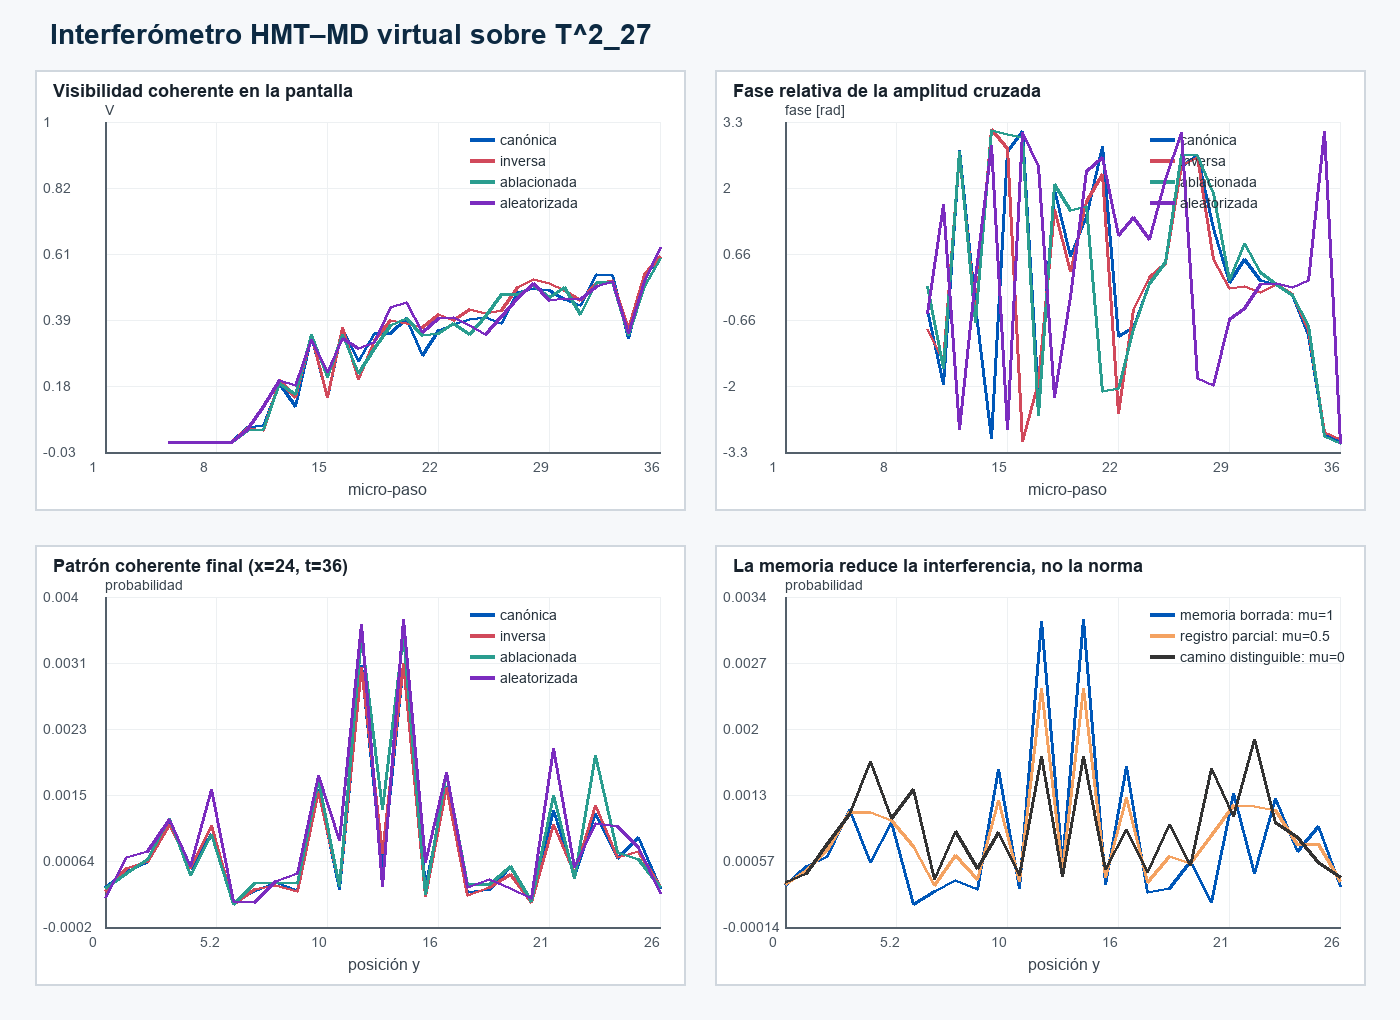
\includegraphics[width=.96\linewidth]{figures/parte_iv/01_curvas_y_patrones.png}
\caption[Évolution de la visibilité, de la phase relative et du motif final pour les quatre séquences à budget commun.]{Évolution de la visibilité, de la phase relative et du motif final pour les quatre séquences à budget commun. \textit{Traduction des libellés de l'image :} « Interféromètre virtuel HMT--MD sur \(T^2_{27}\) ». Panneaux : visibilité cohérente sur l'écran ; phase relative de l'amplitude croisée ; motif cohérent final (\(x=24\), \(t=36\)) ; la mémoire réduit l'interférence, non la norme. Axes : micro-pas, position \(y\), phase [rad], probabilité. Séries : canonique, inverse, avec ablation, aléatoire ; mémoire effacée (\(\mu=1\)), enregistrement partiel (\(\mu=0{,}5\)), chemin discernable (\(\mu=0\)).}
\label{fig:md-sucesora-interferometro-patrones}
\end{figure}

\begin{figure}[tbp]
\centering
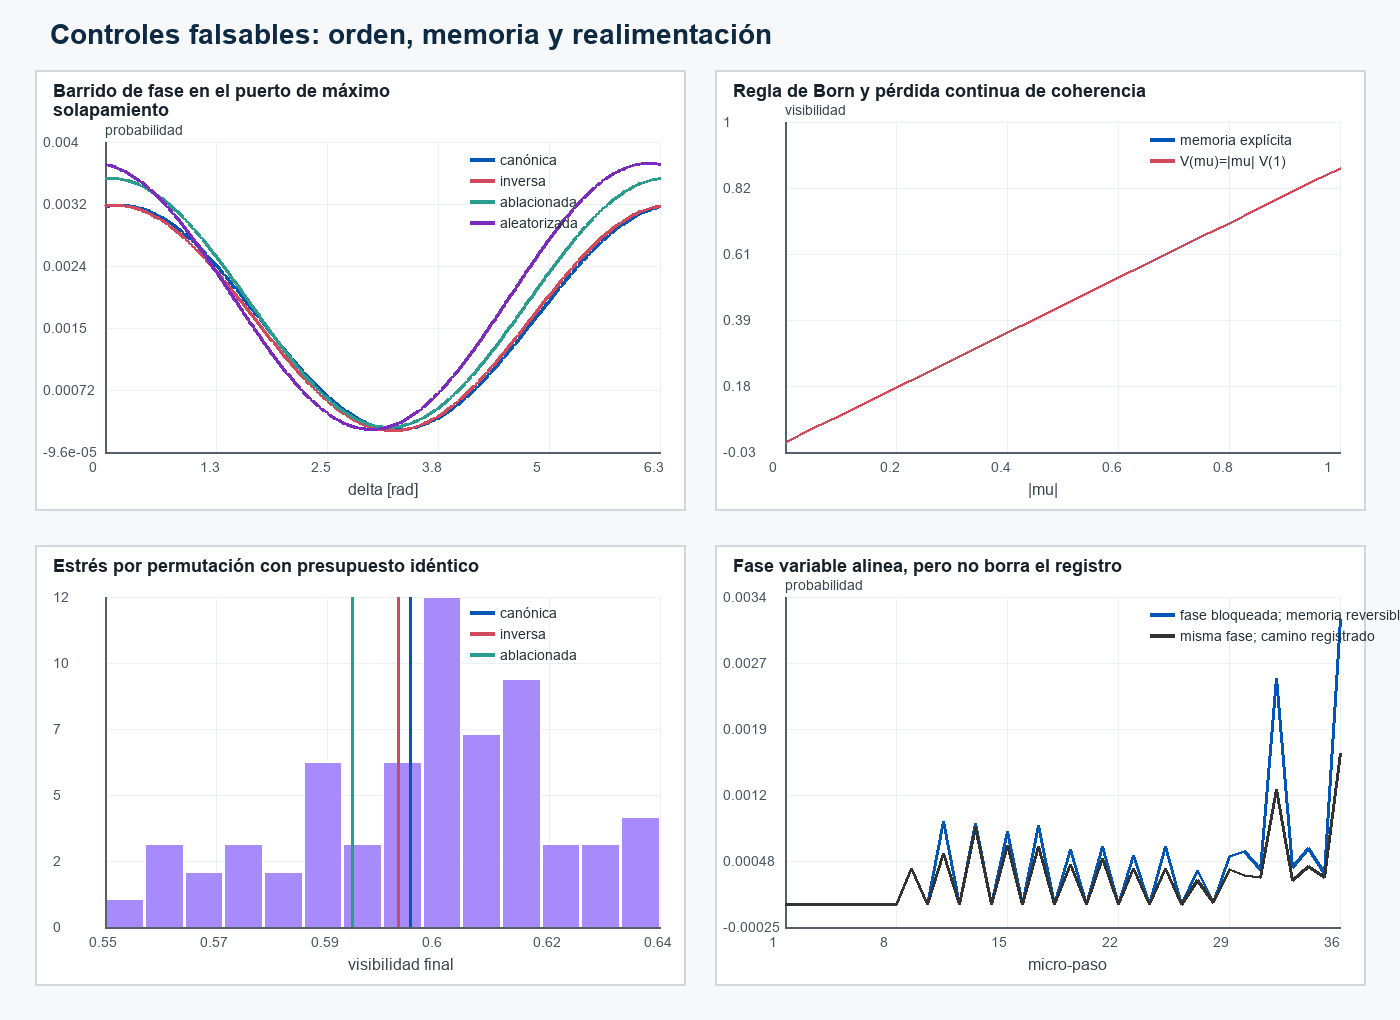
\includegraphics[width=.96\linewidth]{figures/parte_iv/02_estres_memoria_y_control.png}
\caption[Contrôles de l'ordre, de la mémoire de chemin et de la rétroaction de phase.]{Contrôles de l'ordre, de la mémoire de chemin et de la rétroaction de phase. \textit{Traduction des libellés de l'image :} « Contrôles falsifiables d'ordre, de mémoire et de rétroaction ». Panneaux : balayage de phase au port de recouvrement maximal ; règle de Born et perte continue de cohérence ; permutations à budget identique ; la phase variable aligne, mais n'efface pas l'enregistrement. Axes : probabilité, visibilité, \(\delta\) [rad], \(\lvert\mu\rvert\), visibilité finale, micro-pas. Séries : canonique, inverse, avec ablation, aléatoire ; mémoire explicite ; phase verrouillée, mémoire réversible ; même phase, chemin enregistré.}
\label{fig:md-sucesora-interferometro-controles}
\end{figure}

\endgroup

\begingroup
\def\HMTDesiredChapterTitle{Statistiques quantiques d'occupation : distributions de Fermi--Dirac et de Bose--Einstein}%
\let\HMTOriginalChapter\chapter
\renewcommand{\chapter}[2][]{\HMTOriginalChapter{\HMTDesiredChapterTitle}}%
\chapter{Statistiques quantiques d’occupation : distributions de Fermi–Dirac et de Bose–Einstein}
\label{chap:parte-iv-55}

L’énumération microcanonique et les complétions symétrique et antisymétrique produisent les lois de Bose--Einstein et de Fermi--Dirac. La limite de Maxwell--Boltzmann est maintenue comme régime dérivé, et non comme point de départ.

\section{Énumération microcanonique des états sur un écran fini}

Considérons la réalisation finie
\[
 \mathcal H_{\rm occ}=\bigoplus_{k=0}^{3}\CC^{g_k},
 \qquad
 H_{\rm occ}|_{\CC^{g_k}}=E_k^{\rm occ} I,
\]
avec niveaux et multiplicités
\[
 E^{\rm occ}=(0,3,6,9),\qquad g=(1,6,12,8),
 \qquad(N,E)=(12,66).
\]
La somme \(1+6+12+8=27\) fait de \(\mathcal H_{\rm occ}\) un écran à
vingt-sept modes. Ce spectre est la donnée d’une représentation finie
déclarée ; son cardinal ne suffit pas à l’identifier à toute autre
apparition de \(27\) dans HMT\@. Le morphisme qui relie un écran concret
de bord à \((\mathcal H_{\rm occ},H_{\rm occ})\) doit spécifier aussi bien
les fibres que l’opérateur spectral.
Les fonctions génératrices fermionique et bosonique sont
\[
 F(y,x)=\prod_k(1+yx^{E_k^{\rm occ}})^{g_k},
 \qquad
 B(y,x)=\prod_k(1-yx^{E_k^{\rm occ}})^{-g_k}.
\]

\begin{proposition}[Cardinalités microcanoniques]
\label{prop:cardinalidades-microcanonicas}
\[
 [y^{12}x^{66}]F=2\,104\,494,
 \qquad
 [y^{12}x^{66}]B=259\,436\,430.
\]
\end{proposition}
\begin{proof}
Dans le produit fermionique, choisir \(r\) parmi les \(g_k\) modes contribue pour
\(\binom{g_k}{r}y^rx^{rE_k^{\rm occ}}\). Dans le produit bosonique, répartir \(r\)
occupations indiscernables entre \(g_k\) modes contribue pour
\(\binom{g_k+r-1}{r}y^rx^{rE_k^{\rm occ}}\). La convolution finie sur les
quatre niveaux produit les entiers indiqués.
\end{proof}

\section{Distributions de Bose--Einstein et de Fermi--Dirac}

La formulation d’équilibre part du Hamiltonien et du nombre total
d’occupations,
\begin{equation}
 H=\sum_kE_k^{\rm occ} n_k,
 \qquad
 N=\sum_k n_k,
 \qquad
 K_\mu:=H-\mu N.
 \label{eq:hamiltoniano-gran-canonico-rev3}
\end{equation}
Pour \(\beta>0\), l’état grand canonique est
\begin{equation}
 \rho_{\beta,\mu}
 =\frac{e^{-\beta K_\mu}}{\mathcal Z_{\beta,\mu}},
 \qquad
 \mathcal Z_{\beta,\mu}
 =\operatorname{Tr}(e^{-\beta K_\mu}).
 \label{eq:estado-gran-canonico-rev3}
\end{equation}

\begin{theorem}[Factorisation grand canonique et lois d’occupation]
\label{thm:factorizacion-gran-canonica-rev3}
Pour des niveaux d’énergie \(E_k^{\rm occ}\) de dégénérescences \(g_k\), la
trace fermionique se factorise comme
\begin{equation}
 \mathcal Z_{\rm FD}
 =\prod_k\bigl(1+e^{-\beta(E_k^{\rm occ}-\mu)}\bigr)^{g_k},
 \qquad
 \langle n_k\rangle_{\rm FD}
 =\frac{g_k}{e^{\beta(E_k^{\rm occ}-\mu)}+1}.
 \label{eq:factorizacion-fd-rev3}
\end{equation}
Dans le secteur bosonique, sous la condition
\(\mu<\inf_kE_k^{\rm occ}\),
\begin{equation}
 \mathcal Z_{\rm BE}
 =\prod_k\bigl(1-e^{-\beta(E_k^{\rm occ}-\mu)}\bigr)^{-g_k},
 \qquad
 \langle n_k\rangle_{\rm BE}
 =\frac{g_k}{e^{\beta(E_k^{\rm occ}-\mu)}-1}.
 \label{eq:factorizacion-be-rev3}
\end{equation}
\end{theorem}

\begin{proof}
L’opérateur \(K_\mu\) est une somme d’opérateurs d’occupation commutants, de
sorte que sa trace se factorise par modes. Dans chaque mode fermionique, on somme les
occupations \(0\) et \(1\), et le facteur correspondant est
\(1+u_k\), où
\(u_k=e^{-\beta(E_k^{\rm occ}-\mu)}\). Dans chaque mode bosonique, on somme toutes
les occupations non négatives et on obtient la série géométrique
\((1-u_k)^{-1}\) ; la condition sur \(\mu\) garantit \(u_k<1\). Les
puissances \(g_k\) incorporent la dégénérescence. Enfin,
\[
 \langle n_k\rangle
 =-\frac1\beta\frac{\partial}{\partial E_k^{\rm occ}}
   \log\mathcal Z
\]
produit les deux lois d’occupation
\cite{Bose1924,Einstein1924,Fermi1926,Dirac1926,Pathria2011}.
\end{proof}

La dérivation microcanonique retrouve le même résultat dans le régime
thermodynamique. Pour des occupations fermioniques moyennes
\(p_k=m_k/g_k\), l’entropie combinatoire par niveau est
\begin{equation}
 S_k\simeq
 g_k\bigl[-p_k\log p_k-(1-p_k)\log(1-p_k)\bigr].
 \label{eq:entropia-fd-nivel-rev3}
\end{equation}
La variation de \(\sum_kS_k\), soumise à
\(\sum_kg_kp_k=N\) et
\(\sum_kg_kE_k^{\rm occ}p_k=E\), donne
\begin{equation}
 \log\frac{1-p_k}{p_k}=\alpha+\beta E_k^{\rm occ},
 \qquad
 \mu=-\frac{\alpha}{\beta},
 \label{eq:variacion-fd-rev3}
\end{equation}
et, par conséquent, l’occupation de Fermi--Dirac de \eqref{eq:factorizacion-fd-rev3}. Les multiplicateurs \(\beta\) et \(\mu\) sont les coordonnées duales des contraintes d’énergie et de population.

Pour des occupations bosoniques moyennes
\(\overline n_k=m_k/g_k\), la log-multiplicité du niveau est
\begin{equation}
 S_k\simeq
 g_k\bigl[(1+\overline n_k)\log(1+\overline n_k)
          -\overline n_k\log\overline n_k\bigr].
 \label{eq:entropia-be-nivel-rev3}
\end{equation}
La variation de \(\sum_kS_k\), soumise à
\(\sum_kg_k\overline n_k=N\) et
\(\sum_kg_kE_k^{\rm occ}\overline n_k=E\), produit
\begin{equation}
 \log\frac{1+\overline n_k}{\overline n_k}
 =\alpha+\beta E_k^{\rm occ},
 \qquad
 \overline n_k
 =\frac{1}{e^{\beta(E_k^{\rm occ}-\mu)}-1},
 \qquad
 \mu=-\frac{\alpha}{\beta}.
 \label{eq:variacion-be-rev3}
\end{equation}
C’est l’occupation de Bose--Einstein de
\eqref{eq:factorizacion-be-rev3}. La condition
\(\mu<\inf_kE_k^{\rm occ}\) assure la positivité du dénominateur et la
convergence de chaque facteur modal.

Dans l’instance finie construite, les deux contraintes déterminent
\[
 (\beta_{\rm FD},\mu_{\rm FD})
 =(0.15307011353415928,\,4.502865197597043),
\]
\[
 (\beta_{\rm BE},\mu_{\rm BE})
 =(0.05456727960068316,\,-15.92569781906737).
\]
Si \(m_k^{\rm mic}\) désigne l’occupation moyenne obtenue par énumération
microcanonique exacte et \(m_k^{\rm eq}\) l’évaluation de la distribution
correspondante, les erreurs
\(\sum_k|m_k^{\rm mic}-m_k^{\rm eq}|\) sont
\[
 0.09897380039002812\quad\hbox{et}\quad
 0.9190625715582017,
\]
respectivement. L’énumération parcourt tous les quadruplets d’occupation, calcule leurs multiplicités entières et résout les deux équations de contrainte. Les deux lois se réalisent sur un même écran. Le choix physique entre elles exige une graduation et un Hamiltonien compatibles avec la représentation de la trajectoire. Le paramètre thermique sera typé ultérieurement comme \(\beta=(k_B\Theta)^{-1}\).

\section{Convergence quantifiée vers la distribution de Maxwell--Boltzmann}

La relation entre les deux statistiques quantiques et le régime classique peut
être formulée sans recourir à une approximation informelle. Pour chaque mode, soit
\[
 u_k:=e^{-\beta(E_k^{\rm occ}-\mu)}.
\]
Les occupations par état s’écrivent
\[
 \overline n_k^{\rm FD}=\frac{u_k}{1+u_k},
 \qquad
 \overline n_k^{\rm BE}=\frac{u_k}{1-u_k};
\]
les multiplicités \(g_k\) sont incorporées ensuite au moyen de
\(\langle n_k\rangle=g_k\overline n_k\).

\begin{theorem}[Limite classique commune des statistiques quantiques]
\label{thm:limite-clasico-fd-be-rev2}
Si \(0\leq u_k\leq\delta<1\), alors
\[
 \left|\overline n_k^{\rm FD}-u_k\right|\leq u_k^2,
 \qquad
 \left|\overline n_k^{\rm BE}-u_k\right|
 \leq\frac{u_k^2}{1-\delta}.
\]
Par conséquent, dans le régime dilué \(u_k\to0\),
\[
 \boxed{
 \overline n_k^{\rm FD}\sim
 \overline n_k^{\rm BE}\sim
 e^{-\beta(E_k^{\rm occ}-\mu)}} ,
\]
qui est la distribution de Maxwell--Boltzmann par mode.
\end{theorem}

\begin{proof}
Les identités exactes
\[
 u_k-\frac{u_k}{1+u_k}=\frac{u_k^2}{1+u_k},
 \qquad
 \frac{u_k}{1-u_k}-u_k=\frac{u_k^2}{1-u_k}
\]
fournissent les bornes. Pour \(0<u_k\leq\delta\), en divisant par \(u_k\) et
en prenant \(u_k\downarrow0\), on obtient
l’équivalence asymptotique. Le premier terme d’ordre \(u_k^2\) conserve la
différence physique : l’exclusion diminue l’occupation fermionique, tandis que
l’accumulation augmente l’occupation bosonique.
\end{proof}


\section{Complétions quantiques, holonomie de feuillet et périodicité statistique}

Les complétions symétrique et extérieure, la graduation de feuillet, l’holonomie \(2\pi/4\pi\), les dénombrements d’occupation et le complexe cellulaire d’APP forment un unique antécédent algébrique des statistiques quantiques. Le développement intégral est incorporé ici afin que la périodicité ne soit pas réduite à une simple référence ultérieure.

\begingroup
\let\chapter\section
\let\section\subsection
\let\subsection\subsubsection
\let\subsubsection\paragraph
\let\clearpage\relax
\let\cleardoublepage\relax
\chapter{Complétions statistiques et champs sur APP}
\label{chap:completaciones-cuanticas}

Les mots Bose, Fermi, Pauli ou photon ne désignent pas à eux seuls des théorèmes d'un
système discret. Pour les obtenir, il faut spécifier un espace d'états,
une graduation, un produit et des opérateurs. APP et TPK fournissent un ensemble
d'états orientés et une parité de feuillet. À partir de ces données, on peut
construire deux complétions universelles : l'algèbre symétrique et l'algèbre
extérieure. Cette section identifie exactement ce qui découle de la
construction et sépare la statistique algébrique de son interprétation physique.

\section{Espace linéaire des états associé à une réalisation de particule}

Soit \(S\) un ensemble fini de classes de chemins TPK à la profondeur choisie
et soit
\[
 \mathcal H_1=\ell^2(S)
\]
l’espace de Hilbert de base orthonormale \((e_s)_{s\in S}\). Un choix de
poids positifs \(E_s\) définit l’opérateur diagonal
\[
 He_s=E_se_s.
\]
Le choix de \(S\), de son quotient par les symétries et des poids fait partie
du modèle. Une fois ce choix fixé, les complétions multiparticulaires sont canoniques.

\section{Complétions symétrique et extérieure}

On définit
\[
 \mathcal F_+(\mathcal H_1)=
 \bigoplus_{n\geq0}\operatorname{Sym}^n\mathcal H_1,
 \qquad
 \mathcal F_-(\mathcal H_1)=
 \bigoplus_{n\geq0}\bigwedge^n\mathcal H_1.
\]
La première est la complétion bosonique ; la seconde, la fermionique.

\begin{theorem}[Principe d’exclusion de Pauli dans la complétion extérieure]
Pour tout mode \(s\in S\), les opérateurs de création et d'annihilation de la
complétion extérieure satisfont
\[
 \{a_s,a_t^\dagger\}=\delta_{st}I,
 \qquad
 \{a_s,a_t\}=\{a_s^\dagger,a_t^\dagger\}=0.
\]
En particulier, l’opérateur d’occupation
\(N_s=a_s^\dagger a_s\) est un projecteur :
\[
 N_s^2=N_s,
\]
et ses valeurs propres sont \(0,1\).
\end{theorem}

\begin{proof}
La création est le produit extérieur par \(e_s\) ; l'annihilation est son
adjoint. L'antisymétrie implique \(e_s\wedge e_s=0\) et donne les relations
canoniques par calcul sur la base extérieure. Alors
\[
N_s^2=a_s^\dagger a_sa_s^\dagger a_s
=a_s^\dagger(I-a_s^\dagger a_s)a_s=N_s.
\]
Tout projecteur autoadjoint possède un spectre contenu dans \(\{0,1\}\).
\end{proof}

Le principe d'exclusion apparaît ainsi comme un théorème de la complétion
extérieure. La question spécifiquement HMT est de savoir quelle donnée du transport choisit
cette complétion pour une classe de voies.

\section{Graduation de feuillet et algèbre d’échange}

Supposons que le feuillet orienté définit un caractère additif
\[
 p:\operatorname{Mor}(\mathsf P_{\rm TPK})\longrightarrow\mathbb Z/2\mathbb Z,
 \qquad p(\gamma\eta)=p(\gamma)+p(\eta).
\]
Sur l’espace linéaire gradué correspondant, on introduit la symétrie
\[
 \tau(v\otimes w)=(-1)^{p(v)p(w)}w\otimes v.
\]

\begin{theorem}[Complétion statistique déterminée par la parité]
Le quotient de l'algèbre tensorielle par les relations
\[
 v\otimes w-(-1)^{p(v)p(w)}w\otimes v
\]
est symétrique sur le secteur pair et extérieur sur le secteur impair. Deux états
impairs identiques ont un produit nul ; les états pairs admettent une occupation
arbitraire.
\end{theorem}

\begin{proof}
Si \(p(v)=p(w)=0\), la relation est \(vw=wv\). Si
\(p(v)=p(w)=1\), elle est \(vw=-wv\) ; en prenant \(v=w\) et en travaillant en
caractéristique zéro, on obtient \(v^2=0\). Les secteurs mixtes commutent sans
signe supplémentaire. C’est la propriété universelle de l’algèbre symétrique
graduée.
\end{proof}

Le théorème transforme une parité compositionnelle TPK en une règle exacte
d'occupation. Pour obtenir le théorème physique de spin--statistique, il faut
construire en outre une théorie locale lorentzienne positive et démontrer que la
parité de feuillet coïncide avec le spin sous les rotations. L'égalité ne se
déduit pas uniquement du fait que les deux objets prennent des valeurs modulo deux.

\section{Holonomie de feuillet et périodicité de \texorpdfstring{\(2\pi/4\pi\)}{2pi/4pi}}

La parité précédente admet une réalisation géométrique naturelle lorsqu’une
extension survivante possède un retour fermé dont le revêtement d’orientation
est non trivial. Soit \(\rho\) le générateur du retour et soit
\[
 \varepsilon:\langle\rho\rangle\longrightarrow\{-1,+1\}
\]
son caractère d’holonomie, avec \(\varepsilon(\rho)=-1\). Le fibré réel
associé est alors la droite d’orientation d’une bande de Möbius : un
tour ferme la projection géométrique, mais change le feuillet relevé ; deux
tours restaurent l’orientation.

Pour écrire cette propriété angulairement, fixons une représentation
unitaire \(U\) du revêtement des rotations sur l’espace gradué
\(\mathcal H_1=\mathcal H_{\bar0}\oplus\mathcal H_{\bar1}\), compatible avec
la parité de feuillet au sens
\[
 U(2\pi)v=(-1)^{p(v)}v
\]
pour tout vecteur homogène \(v\). La compatibilité est une condition de la
réalisation : elle identifie le générateur du revêtement d’orientation au
caractère \(p\) déjà construit sur les chemins.

\begin{theorem}[Restauration de l’orientation et algèbre d’échange]
\label{thm:dos-cuatro-pi-estadistica}
Sous la compatibilité précédente,
\[
 U(2\pi)|_{\mathcal H_{\bar0}}=I,
 \qquad
 U(2\pi)|_{\mathcal H_{\bar1}}=-I,
 \qquad
 U(4\pi)=I.
\]
En outre, le même caractère \(p\) détermine la symétrie graduée
\[
 \tau(v\otimes w)=(-1)^{p(v)p(w)}w\otimes v.
\]
Par conséquent, le secteur d’holonomie paire est complété au moyen de puissances
symétriques et le secteur d’holonomie impaire au moyen de puissances extérieures. Dans
le second, l’exclusion \(v\wedge v=0\) est satisfaite.
\end{theorem}

\begin{proof}
La première et la seconde égalité sont la condition de compatibilité évaluée
dans chaque composante homogène. En itérant un tour,
\[
 U(4\pi)v=U(2\pi)^2v=(-1)^{2p(v)}v=v,
\]
ce qui démontre la restauration. L'affirmation sur l'échange est le
théorème de complétion par parité de la section précédente : pour deux vecteurs
pairs, le signe est positif, tandis que pour deux impairs, il est négatif.
\end{proof}

Il convient de distinguer trois retours. La clôture angulaire après \(2\pi\) est un
retour de la projection ; la clôture après \(4\pi\) restaure l’orientation
relevée ; aucune n’oblige à elle seule toutes les coordonnées du registre à
revenir à leur valeur initiale. Cette séparation est l’analogue dimensionnel de la
distinction HMT entre retour de phase et retour d’état.

\subsection{Les feuillets somme et produit comme supports des \(2\) complétions}

Le tableau APP contient deux évaluations sur un même support. Le feuillet
additif agit par translations et conserve la multiplicité des
continuations ; en ce sens, il accumule. Le feuillet multiplicatif est
permutatif sur les unités et contracte des fibres sur les non-inversibles ; en
ce sens, il plie. Cette incompatibilité est antérieure au choix
statistique et explique pourquoi TPK doit conserver deux généalogies au lieu de
les réduire à un seul mot visible.

L’attribution statistique ne s’obtient toutefois pas en remplaçant
verbalement « somme » par « boson » et « produit » par « fermion ». L’application exacte est
le caractère de parité
\[
 p:\operatorname{Mor}(\mathsf P_{\rm TPK})\longrightarrow\mathbb Z/2\mathbb Z.
\]
Lorsque le transport d’une extension tombe dans le secteur \(p=0\), sa
complétion admet une occupation cumulative et est symétrique. Lorsqu’il tombe dans
\(p=1\), l’inversion de feuillet introduit le signe d’échange et la
complétion est extérieure. La somme et le produit fournissent les deux
géométries locales ; le registre, l’orientation et le caractère \(p\) décident dans
quel secteur un chemin est réalisé.

Avec un hamiltonien diagonal \(H\), une énergie \(\epsilon\), un potentiel chimique
\(\mu\) et un paramètre thermique \(\beta\), les occupations moyennes des deux
secteurs sont alors
\[
 \bar n_{\rm par}(\epsilon)
 =\frac{1}{e^{\beta(\epsilon-\mu)}-1},
 \qquad
 \bar n_{\rm impar}(\epsilon)
 =\frac{1}{e^{\beta(\epsilon-\mu)}+1}.
\]
Les formules de Bose--Einstein et de Fermi--Dirac sont donc les
évaluations thermodynamiques des complétions symétrique et extérieure
sélectionnées par le transport. La périodicité \(4\pi\) et l'exclusion
fermionique sont coordonnées par le même caractère, mais aucune des deux
ne s'infère d'une simple coïncidence numérique.

\section{Opérateurs de nombre et distribution d'occupation dans la réalisation de Fock}

S’il y a \(g\) modes et \(N\) particules, les dimensions des secteurs sont
\[
 \Omega_F(g,N)=\binom gN,
 \qquad
 \Omega_B(g,N)=\binom{g+N-1}{N}.
\]
La première formule compte les sous-ensembles de modes ; la seconde, les compositions
faibles de \(N\) en \(g\) parties. Ces comptages sont des conséquences exactes des
deux complétions et ne requièrent pas d'hypothèse thermodynamique.

\section{Le complexe cellulaire du tore APP}

Le graphe de APP est le squelette de dimension un d’une décomposition cellulaire du tore
\(T^2\) à \(9\times9\) sommets. Soit
\[
 C^0\xrightarrow{d_0}C^1\xrightarrow{d_1}C^2
\]
son complexe de cochaînes réelles. Le produit scalaire uniforme étant choisi,
nous définissons la codifférentielle \(\delta=d^*\) et le laplacien
\[
 \Delta_k=d_{k-1}\delta_k+\delta_{k+1}d_k.
\]

\begin{theorem}[Secteur harmonique du tore numérique]
La dimension de l'espace des un-formes harmoniques est deux :
\[
 \dim\ker\Delta_1=b_1(T^2)=2.
\]
On peut choisir une base représentée par les flux uniformes horizontal et
vertical. Les deux sont fermés, cofermés et ne sont pas des gradients de fonctions
globales périodiques.
\end{theorem}

\begin{proof}
Le théorème de Hodge pour les complexes cellulaires finis identifie
\(\ker\Delta_1\) à \(H^1(T^2;\mathbb R)\). La cohomologie du tore est de
rang deux. Directement, les flux constants horizontal et vertical ont
une divergence et un rotationnel nuls ; leurs intégrales sur les deux cycles
fondamentaux sont indépendantes, de sorte qu’ils ne sont pas exacts.
\end{proof}

L’espace des connexions modulo les transformations de jauge est
\[
 C^1/\operatorname{im}d_0.
\]
Dans un complexe fini muni du produit scalaire précédent, chaque orbite
admet un représentant de Coulomb dans \(\ker\delta_1\) ; à l’intérieur de l’orbite,
le choix est unique modulo le stabilisateur \(\ker d_0\) du paramètre de
jauge. Le quotient cohomologique correct est
\[
 \ker d_1/\operatorname{im}d_0
 \simeq \ker\Delta_1 .
\]
Ses deux classes harmoniques constituent un candidat mathématique naturel pour
deux modes globaux libres. Ce ne sont pas encore les deux polarisations locales d’un
photon dans l’espace-temps \(3+1\) : cette identification nécessite une
limite dynamique, une relation de dispersion et un groupe physique de jauge.

\section{Loi de Gauss discrète}

Pour une 1-cochaîne orientée \(F\) et un ensemble de sommets \(V\), la
divergence est définie par
\[
 (\operatorname{div}F)(v)=
 \sum_{e:v\to w}F(e)-\sum_{e:w\to v}F(e).
\]
En sommant sur \(V\), toute arête intérieure apparaît une fois avec chaque signe et
s’annule. Par conséquent,
\[
 \boxed{
 \sum_{v\in V}\operatorname{div}F(v)
 =\operatorname{Flux}_{\partial V}(F).}
\]
Cette identité est une loi de Gauss exacte sur le graphe. Interpréter
\(\operatorname{div}F\) comme une charge électrique exige le caractère de charge et la
réalisation dimensionnelle construits en mécanique dimensionnelle.

\section{Appareil de mesure réversible}

Soit \(S\) un ensemble d’états et soit \(r:S\to\mathbb Z/9\mathbb Z\) une
lecture. Le couplage à un registre nonadique est défini par
\[
 U_r:S\times\mathbb Z/9\mathbb Z\longrightarrow
 S\times\mathbb Z/9\mathbb Z,
 \qquad
 U_r(s,a)=(s,a+r(s)).
\]

\begin{proposition}[Réversibilité du couplage]
L'application \(U_r\) est une permutation et
\[
 U_r^{-1}(s,a)=(s,a-r(s)).
\]
La perte d’information n’apparaît qu’après l’application d’un lecteur au
registre ou le conditionnement de l’état par le résultat.
\end{proposition}

\begin{proof}
La formule proposée pour l’inverse satisfait les deux compositions par la
loi de groupe de \(\mathbb Z/9\mathbb Z\).
\end{proof}

Cette proposition formalise la définition opératoire de la mesure : coupler,
lire et restreindre les futurs compatibles sont trois applications différentes. Le
couplage complet est réversible ; le quotient observationnel peut ne pas l’être.

\section{Correspondances algébriques et réalisations physiques}

Les complétions de Fock, l’exclusion conditionnée à la parité, le secteur
harmonique de APP, la loi de Gauss discrète et la réversibilité de l’appareil sont des théorèmes
mathématiques complets. Leurs identifications physiques forment un diagramme qui
doit commuter :
\[
 \text{parité de feuillet}
 \longrightarrow\text{échange gradué}
 \longrightarrow\text{CAR/CCR}
 \longrightarrow\text{statistique physique},
\]
\[
 H^1(\mathcal A_9)
 \longrightarrow\text{champ discret de jauge}
 \longrightarrow\text{mode sans masse}
 \longrightarrow\text{photon}.
\]
Les deux premières flèches de chaque ligne possèdent des constructions explicites ; les
dernières requièrent la dynamique et la limite physique correspondantes. Cette
séparation permet de développer les ponts sans confondre une analogie de
cardinalité avec une représentation.

\endgroup

\paragraph{De la mesure réversible à l’occupation fermionique et au principe algébrique d’exclusion de Pauli} La distinction statistique est complétée algébriquement par l’idempotence d’occupation et l’exclusion fermionique.

\endgroup
% Contenido exclusivo del propietario de entropías tipadas.
\subsection{Corrélation quasi libre et entropies spectrales d’occupation}

Pour un état fermionique quasi libre invariant de jauge, conservant le
nombre et défini sur un espace à un corps de dimension finie, soit
\(C_{ij}=\langle a_j^\dagger a_i\rangle\) l’opérateur de corrélation à un
corps. L’hypothèse d’invariance de jauge exclut les corrélations anormales
d’appariement, de sorte que \(C\) détermine l’état quasi libre. Si
\(0<C<I\), son générateur modulaire à un corps et la reconstruction réciproque
du corrélateur sont
\begin{equation}
 \boxed{
 K_1=\log\bigl((I-C)C^{-1}\bigr),
 \qquad
 C=(I+e^{K_1})^{-1}.}
 \label{eq:puente-cuasilibre-modular-rev3}
\end{equation}

\begin{corollary}[Forme logistique du spectre modulaire]
\label{cor:forma-logistica-modular-rev3}
Si \(K_1u_i=\kappa_i u_i\), l’occupation du mode \(u_i\) est
\[
 \langle n_i\rangle=\frac1{1+e^{\kappa_i}}.
\]
Pour \(\kappa_i=\beta(\varepsilon_i-\mu)\), on retrouve la loi de
Fermi--Dirac.
\end{corollary}

\begin{proof}
La diagonalisation spectrale de \(K_1\) diagonalise toute fonction de cet opérateur.
L’application de \(x\mapsto(1+e^x)^{-1}\) à chaque valeur propre produit la formule.
\end{proof}

Si \(C\) a pour valeurs propres \(p_i\in[0,1]\), l’entropie d’occupation de
l’état fermionique quasi libre est, avec la convention \(0\log0=0\),
\begin{equation}
 S_F=-\sum_i\bigl[p_i\log p_i+(1-p_i)\log(1-p_i)\bigr].
 \label{eq:entropia-cuasilibre-fermi-rev3}
\end{equation}
Pour un état bosonique gaussien diagonal avec un nombre fini de modes et
des occupations moyennes \(\overline n_i\),
\begin{equation}
 S_B=\sum_i\bigl[(1+\overline n_i)\log(1+\overline n_i)
                  -\overline n_i\log\overline n_i\bigr].
 \label{eq:entropia-gaussiana-bose-rev3}
\end{equation}
La même formule s'étend à une famille dénombrable lorsque la série du
membre de droite converge.
Ces entropies quantifient des configurations d'occupation. L'entropie d'
intrication possède un autre domaine : l'état réduit induit par une
décomposition tensorielle. Leur identification requiert de déclarer la
réduction et l'opérateur de corrélation qui les implémentent.

Enfin, pour un état réduit \(\rho_A\), l’\emph{entropie de von
Neumann}
\[
 S_{\rm vN}(\rho_A)=-\operatorname{Tr}(\rho_A\log\rho_A)
\]
est une propriété spectrale de l'opérateur de densité. Lorsque \(\rho_A\)
provient d'une purification globale, elle quantifie l'intrication à travers
la coupure. Dans la construction de bord HMT, l'opérateur d'aire, l'
hamiltonien modulaire et la réduction correspondante demeurent dans la
\cref{hap:sec:area-entrelazamiento-barbero-rev11}.

Les applications entre ces domaines sont publiées par des identités explicites.
La décomposition d'une mesure par les fibres de \(q\) satisfait la règle de
chaîne
\begin{equation}
 \mathsf H_\mu(\mathbf X)
 =\mathsf H_{q_*\mu}(q(\mathbf X))
  +\mathsf H_{\rm fib}(q;\mu).
 \label{eq:cadena-entropia-fibras-rev2}
\end{equation}
\Needspace{5\baselineskip}
Une distribution finie \(p=(p_i)\) se réalise diagonalement comme
\[
 \rho_p=\sum_i p_i|i\rangle\langle i|,
 \qquad S_{\rm vN}(\rho_p)=\mathsf H(p).
\]
Si \(P_{N,E}\) projette sur le sous-espace microcanonique de dimension
\(\Omega(N,E)\), alors
\[
 \rho_{\rm mc}=\frac{P_{N,E}}{\Omega(N,E)},
 \qquad S_{\rm vN}(\rho_{\rm mc})=\log\Omega(N,E)=S_{\rm mc}.
\]
Pour un état pur bipartite,
\[
 \rho_A=\operatorname{Tr}_B
 \bigl(|\Psi_{AB}\rangle\langle\Psi_{AB}|\bigr)
\]
définit la réduction qui mesure l'intrication. Enfin, l'égalité entre
\(h_{\rm top}=\log\rho(A)\) et une entropie métrique est atteinte, pour ce
système primitif, par la mesure de Parry, qui réalise l'entropie métrique
maximale ; elle n'est pas attribuée à une mesure arbitraire d'histoires.



\begingroup
\def\HMTDesiredChapterTitle{Complétion fermionique des trajectoires et principe algébrique d’exclusion de Pauli}%
\let\HMTOriginalChapter\chapter
\renewcommand{\chapter}[2][]{\HMTOriginalChapter{\HMTDesiredChapterTitle}}%
\chapter{Complétion fermionique des trajectoires et principe algébrique d’exclusion de Pauli}
\label{chap:parte-iv-56}

La complétion extérieure des trajectoires impose l’idempotence et l’exclusion avant toute identification d’espèce. Les caractères de rotation, de couleur, de saveur et de virtualité conservent leur typage dans la représentation correspondante.

\section{Occupation, exclusion et statistique finie}
\label{chap:ocupacion-estadistica}
\index{Pauli, principe d’exclusion de}\index{CAR}
\index{Fermi--Dirac}\index{Bose--Einstein}

Les réalisations nulle et matérielle fournissent le support géométrique de l’occupation. Le secteur fermionique est construit sur les relations canoniques d’anticommutation (CAR), et le théorème spin--statistique exige en outre la représentation opératorielle déclarée. Cette section fixe ces prémisses avant de dériver l’idempotence de l’occupation, les cardinalités microcanoniques et les distributions de Bose--Einstein et de Fermi--Dirac avec leur limite classique commune.

\subsection{Idempotence de l’occupation dans l’algèbre d’anticommutation}

Soient \(a_i,a_i^\dagger\) des opérateurs satisfaisant les relations canoniques d’anticommutation (CAR)
\[
 \{a_i,a_j^\dagger\}=\delta_{ij},
 \qquad \{a_i,a_j\}=0,
\]
et soit \(n_i=a_i^\dagger a_i\).

\begin{theorem}[Principe d’exclusion de Pauli]
\label{thm:principio-exclusion-pauli}
On a \(n_i^2=n_i\), et donc \(\Spec(n_i)\subseteq\{0,1\}\).
\end{theorem}
\begin{proof}
\[
 n_i^2=a_i^\dagger a_i a_i^\dagger a_i
 =a_i^\dagger(1-a_i^\dagger a_i)a_i
 =a_i^\dagger a_i,
\]
car \(a_i^2=(a_i^\dagger)^2=0\). Toute valeur propre d’un idempotent satisfait \(\lambda^2=\lambda\) \cite{Pauli1925,Dirac1926}.
\end{proof}

La nilpotence \((a_i^\dagger)^2=0\) interdit la double occupation fermionique d’un même mode et conduit, par maximisation de l’entropie sous les contraintes d’énergie et de nombre, à la loi d’occupation de Fermi--Dirac exposée plus loin. La complétion symétrique et la loi de Bose--Einstein constituent une strate distincte et sont présentées séparément.

Les relations CAR sont une hypothèse algébrique du théorème. Une monodromie avec changement de signe sous une rotation de \(2\pi\) est compatible avec une représentation fermionique, mais ne constitue pas à elle seule une dérivation de CAR ni du théorème spin--statistique.


\section{Caractères de rotation, couleur, saveur et virtualité}

Soit \(\jmath:\Gamma_{\rm TPK}\to\Gamma_{\rm TPK}\) l’involution qui inverse l’orientation de chaque arête et permute les fibres au moyen de \(J_c:E_c\to E_{\jmath c}\). Un caractère de rotation est une représentation \(\rho_{\rm rot}\) du sous-groupe engendré par \(\jmath\) sur les sections ; ses sous-espaces propres de signes \(+1\) et \(-1\) sont des objets algébriques distincts d’une représentation physique du groupe de Lorentz.

Soit \(\mathcal C\) le groupe abélien des caractères de canal du transport. Deux sections possèdent la même \emph{saveur arithmétique} lorsque leurs caractères
\[
 \chi_s:\mathcal C\longrightarrow\CC^\times
\]
coïncident. L’identification de ces classes à des saveurs de fermions exige une représentation de l’algèbre des observables physiques et n’est pas introduite par la nomenclature.

Enfin, soit
\[
 \operatorname{Ext}_N(s)=
 \{s'\in\Gamma(\mathcal B_{\gamma'}):
 \gamma'|_{\{0,\ldots,N\}}=\gamma,\ s'|_{\{0,\ldots,N\}}=s\}.
\]
La section est stable à partir de la profondeur \(N\) lorsque les restrictions \(\operatorname{Ext}_{N+1}(s)\to\operatorname{Ext}_N(s)\) admettent une branche compatible à tout niveau ultérieur. Elle est dite \emph{virtuelle jusqu’à la profondeur \(N\)} lorsque cette branche globale n’existe pas encore, bien que des extensions finies subsistent. Cette définition relève du système inverse et ne dépend pas d’une métaphore temporelle.

Sur le plan affine \(\FF_3^2\), la fonctionnelle linéaire
\[
 \kappa_3:\FF_3^2\longrightarrow\FF_3,
 \qquad \kappa_3(r,c)=r-c
\]
est surjective et son noyau est de dimension un. Ses trois fibres sont donc les classes affines du noyau et contiennent chacune exactement trois points. Le même équilibre persiste dans toute réunion disjointe de copies complètes de \(\FF_3^2\). Cette partition ternaire est une assertion algébrique autonome. La carte qutrit, l’orientation et le caractère de phase étant fixés, \cref{chap:algebra-color-qutrit} construit la représentation et son algèbre \(\mathfrak{su}(3)\) ; l’entrelaceur avec le transport TPK et l’identification chromodynamique physique demeurent une interface.


\paragraph{Distinction entre transport généalogique réversible et projection irréversible.} La réversibilité de la mise à jour permet de distinguer le coût d’une projection irréversible du transport généalogique complet.

\endgroup

\begingroup
\def\HMTDesiredChapterTitle{Mise à jour réversible, coût d’effacement et domaine exact de la limite nulle de Landauer}%
\let\HMTOriginalChapter\chapter
\renewcommand{\chapter}[2][]{\HMTOriginalChapter{\HMTDesiredChapterTitle}}%
\chapter{Mise à jour réversible, coût d’effacement et domaine exact de la limite nulle de Landauer}
\label{chap:parte-iv-57}

Le transport complet conserve l’information de fibre et peut avoir un coût logique nul ; la projection ou la réinitialisation qui écarte la généalogie est soumise au coût de Landauer. Les deux domaines sont explicitement séparés.

\section{Réversibilité logique et principe de Landauer dans les fibres de TPK}
\label{sec:informacion-fibra-landauer-rev7}
\index{Landauer}\index{information!fibre}

Soit \((\Omega,2^\Omega,\mu)\) un espace probabilisé fini, soit \(X:\Omega\to\mathcal X\) une variable aléatoire à valeurs dans l’espace \(\mathcal X\) des états complets et soit \(q:\mathcal X\to Y\) un lecteur. La règle de chaîne donne
\[
 \mathsf H(X)
 =
 \mathsf H(q(X))+\mathsf H(X\mid q(X)).
\]
Le deuxième terme mesure l’information de la fibre que le lecteur n’exprime pas.

\begin{theorem}[Coût de Landauer nul pour le transport complet et coût de la projection]
\label{thm:landauer-relativo-lector-rev7}
Si \(U:\mathcal X\to\mathcal X\) est une mise à jour bijective de l’état HMT complet, alors
\[
 \boxed{\mathsf H(X\mid U(X))=0.}
\]
Pour une sortie projetée \(q(U(X))\), l’information écartée est
\[
 \mathsf H(X\mid q(U(X))).
\]
Une réinitialisation physique qui identifie des états distincts de la mémoire doit comptabiliser cette information dans l’environnement.
\end{theorem}

\begin{proof}
La bijectivité implique \(X=U^{-1}(U(X))\) ; \(X\) est donc déterminé par \(U(X)\) et l’entropie conditionnelle est nulle. Pour le lecteur \(q\), la règle de chaîne sépare l’entropie exprimée de l’entropie de la fibre. Si l’opération de réinitialisation n’est pas injective, la sortie ne permet plus de reconstruire l’état de mémoire. Le principe thermodynamique de Landauer borne le coût de l’implémentation en fonction de cette entropie effacée ; la mise à jour réversible ne fournit pas à elle seule de terme d’effacement.
\end{proof}

En nats et en bits, respectivement,
\[
 Q\ge k_B\Theta\,\mathsf H_{\rm nat},
 \qquad
 Q\ge k_B\Theta\log 2\,\mathsf H_{\rm bit}.
\]
Pour le transport bijectif de l’état complet, l’entropie d’effacement est nulle ; le terme minimal de Landauer associé exclusivement à l’effacement satisfait donc
\[
\boxed{Q_{\rm L}^{\min}[U]=k_B\Theta\,
 \mathsf H(X\mid U(X))=0.}
\]
Pour la réinitialisation d’un TRIT uniforme, en revanche,
\[
 \boxed{Q_{\rm reset}\ge k_B\Theta\log3.}
\]
Ces deux équations situent le coût dans la perte d’information : le coût apparaît lorsque la projection ou la réinitialisation oublie la fibre. La préparation, la projection et la réinitialisation peuvent produire de l’entropie ; le transport réversible conserve l’information généalogique. La valeur nulle est la limite logique de Landauer pour cette mise à jour complète, tandis que les coûts dynamiques de contrôle, de vitesse finie et de couplage à l’environnement relèvent de la réalisation physique du dispositif.

\begin{statusbox}[title={Portée du coût de Landauer nul}]
L’égalité \(\mathsf H(X\mid U(X))=0\) est exacte pour une mise à jour bijective de l’état enrichi. La borne \(Q_{\rm reset}\ge k_B\Theta\log3\) est la spécialisation de Landauer à l’effacement d’une décision triadique uniforme. La réalisation des deux formules en joules utilise le transducteur de Boltzmann et une température physique déclarée.
\end{statusbox}


\paragraph{Transduction de l’information de bord en capacité de la coupe triadique minimale.} L’information conservée par le bord réapparaît géométriquement dans la coupe triadique minimale et dans sa capacité.

\endgroup
\begingroup
\let\HMTOwnerSection\section
\let\HMTOwnerSubsection\subsection
\let\HMTOwnerSubsubsection\subsubsection
\let\HMTOwnerParagraph\paragraph
\let\chapter\HMTOwnerSection
\let\section\HMTOwnerSubsection
\let\subsection\HMTOwnerSubsubsection
\let\subsubsection\HMTOwnerParagraph
\chapter{Conservation généalogique de l'information, entropies de réduction et structure thermique}
\label{chap:informacion-entropia-landauer}

L'information que transporte un état HMT ne se réduit pas à la coordonnée que
publie l'un de ses lecteurs. La coordonnée visible, le feuillet, l'orientation,
le quotient, la retenue, le chemin et le sceau de clôture appartiennent au même
état enrichi, bien qu'une évaluation concrète n'en montre qu'une partie.
Cette distinction permet de situer dans un cadre unique trois opérations que la
description macroscopique présente habituellement séparément : conserver une histoire,
la réduire à une lecture et attribuer une énergie à l'information effectivement
effacée.

Le chapitre développe cette chaîne sans identifier ses échelons. On
formule d'abord la mémoire de la fibre et le critère exact de récupérabilité. Ensuite,
on démontre la nullité du terme logique de Landauer pour une mise à jour
bijective de l'état enrichi du TPK. On distingue alors cinq
entropies qui possèdent des domaines et des fonctions différents. Enfin, le quotient
aréal--volumétrique et l'horloge de \(108\) pas fournissent la structure qui
relie information triadique, action et température.

\section{Désintégration de la lecture visible sur les fibres et récupération de la mémoire généalogique}

Soit \(\Omega\) un espace fini d'états enrichis et soit
\[
 q:\Omega\longrightarrow Y
\]
un lecteur visible. La valeur \(q(x)\) est une coordonnée de l'état \(x\), non sa
description exhaustive. Notons
\[
 M:\Omega\longrightarrow\mathcal M
\]
le registre conjoint des coordonnées généalogiques que le lecteur ne publie pas :
feuillet, orientation, quotient ou retenue, phase, chemin et sceau, selon le domaine
considéré.

\begin{definition}[Lecteur enrichi et mémoire de fibre]
Le lecteur enrichi associé à \(q\) et \(M\) est
\begin{equation}
 \widehat q=(q,M):\Omega\longrightarrow Y\times\mathcal M.
 \label{eq:lector-enriquecido-informacion}
\end{equation}
La mémoire de fibre de \(q\) est l'information nécessaire pour distinguer les
états contenus dans une même fibre \(q^{-1}(y)\).
\end{definition}

L'extension résidu--quotient d'APP est l'exemple arithmétique élémentaire. Dans
chaque cellule, les deux divisions euclidiennes sont conservées
\[
 i+j=9q^+_{ij}+R^+_{ij},
 \qquad
 ij=9q^\times_{ij}+R^\times_{ij}.
\]
La réduction modulo neuf publie \(R^+\) ou \(R^\times\) ; le relèvement
conserve simultanément \((R,q)\). En sommant sur le domaine nonadique, on
obtient l'identité exacte
\begin{equation}
 2025-810
 =54+9\cdot129.
 \label{eq:app-residuo-cociente-informacion}
\end{equation}
Le premier terme à droite est la différence entre les résidus visibles ;
le deuxième recompose la différence entre les quotients. L'égalité démontre
que la projection résiduelle ne détermine pas à elle seule l'opération entière.

Soit maintenant \(X\) une variable aléatoire à valeurs dans \(\Omega\). Nous travaillerons
avec des entropies adimensionnelles en nats. La règle de la chaîne donne
\begin{equation}
 \mathsf H(X)
 =\mathsf H(q(X))+\mathsf H(X\mid q(X)).
 \label{eq:cadena-entropia-fibra}
\end{equation}
Le deuxième terme quantifie l'information généalogique qui subsiste à l'intérieur
de la fibre de la lecture.

\begin{theorem}[Récupérabilité par mémoire de fibre]
\label{thm:recuperabilidad-memoria-fibra}
Si le lecteur enrichi \(\widehat q=(q,M)\) est injectif sur le support de
\(X\), alors
\begin{equation}
 \boxed{\mathsf H(X\mid q(X),M(X))=0.}
 \label{eq:entropia-condicional-memoria-cero}
\end{equation}
L'entropie \(\mathsf H(X\mid q(X))\) mesure exactement l'information qui serait
perdue en conservant la coordonnée visible et en écartant la mémoire.
\end{theorem}

\begin{proof}
L'injectivité de \(\widehat q\) fournit une inverse sur son image. Par
conséquent, la paire \((q(X),M(X))\) détermine \(X\) et l'entropie conditionnelle est
nulle. Si l'on omet \(M(X)\), les entrées d'une même fibre sont
identifiées ; la règle de la chaîne \eqref{eq:cadena-entropia-fibra} attribue à
cette identification le terme \(\mathsf H(X\mid q(X))\).
\end{proof}

La définition généalogique du nombre s'insère précisément ici. Un nombre
HMT est une section compatible de cylindres survivants, accompagnée de la mémoire
de son chemin, de son orientation, de sa signature et de sa clôture. Sa valeur réelle est l'évaluation de cette
section. L'évaluation peut oublier des coordonnées ; la section les conserve.

\section{Réversibilité logique et terme de Landauer}

Soit
\[
 U:\Omega\longrightarrow\Omega
\]
une mise à jour de l'état enrichi du TPK. La question de Landauer se
formule sur l'application complète, avant d'appliquer un lecteur visible ou de réinitialiser
un registre ; sa formulation thermodynamique de l'effacement logique remonte à
Landauer \cite{Landauer1961}.

\begin{theorem}[Landauer nul pour le transport complet]
\label{thm:landauer-nulo-tpk-anexo}
Si \(U\) est bijective, alors, pour toute distribution d'entrée \(X\),
\begin{equation}
 \mathsf H(X\mid U(X))=0.
 \label{eq:landauer-entropia-cero-anexo}
\end{equation}
Dans le régime idéal de Landauer, le terme minimal associé exclusivement à
l'effacement logique interne est
\begin{equation}
 \boxed{
 Q_{\rm L}^{\min}[U]
 =k_B\Theta\,\mathsf H(X\mid U(X))=0.}
 \label{eq:landauer-nulo-anexo}
\end{equation}
\end{theorem}

\begin{proof}
La bijection fournit \(U^{-1}\), de sorte que
\(X=U^{-1}(U(X))\). La sortie complète détermine l'entrée et l'entropie
conditionnelle s'annule. La forme informationnelle du principe de Landauer attribue
le coût d'effacement au terme \(k_B\Theta\mathsf H(X\mid U(X))\), qui, par
l'égalité précédente, vaut zéro.
\end{proof}

Le résultat localise la conservation dans l'espace enrichi. Pour une
sortie projetée \(q(U(X))\), l'information non publiée est
\begin{equation}
 \mathsf H\bigl(X\mid q(U(X))\bigr).
 \label{eq:informacion-proyeccion-anexo}
\end{equation}
Une réinitialisation physique qui identifie des états distincts doit transférer cette
information à l'environnement. En particulier, la réinitialisation d'un TRIT uniforme vers un unique
état possède
\[
 \mathsf H(X)=\log3,
 \qquad
 \boxed{Q_{\rm reset}\geq k_B\Theta\log3.}
\]
La mise à jour réversible, la projection et la réinitialisation sont ainsi des opérations
distinctes. La première conserve la généalogie ; la deuxième réduit la lecture ; la
troisième élimine physiquement un registre. La dissipation supplémentaire due au
contrôle, au bruit ou à une vitesse finie appartient à la réalisation du
dispositif et non au terme logique d'effacement de
\eqref{eq:landauer-nulo-anexo}.

\section{\(5\) notions d'entropie et leurs domaines}

Le mot \emph{entropie} désigne dans cette construction cinq fonctionnelles
liées, mais non interchangeables. Leur séparation évite d'attribuer une température
à un dénombrement purement combinatoire ou une perte d'information à une évolution
qui ne fait que changer de lecture.

\subsection{Entropie conditionnelle des fibres du lecteur visible et perte de généalogie}

La quantité
\[
 \mathsf H_{\rm fib}(q;X):=\mathsf H(X\mid q(X))
\]
mesure l'information de la généalogie qu'une lecture visible ne distingue pas.
Son domaine est un lecteur et une distribution sur l'état enrichi. Elle
s'annule lorsque le lecteur est fidèle sur le support considéré.

\subsection{Entropie informationnelle d'une décision triadique}

Pour une distribution \(p=(p_{-1},p_0,p_{+1})\) sur les trois états
visibles du TRIT,
\[
 I_{\rm TRIT}(p)=-\sum_{a\in\{-1,0,+1\}}p_a\log p_a.
\]
La distribution uniforme produit
\begin{equation}
 \boxed{I_{\rm TRIT}=\log3.}
 \label{eq:informacion-trit-log3-anexo}
\end{equation}
Cette quantité mesure une décision locale entre trois alternatives visibles.

\subsection{Entropie topologique des histoires admissibles}

Si \(A\) est la matrice d'adjacence d'un sous-shift fini, son entropie
topologique est
\[
 h_{\rm top}(A)=\log\rho(A),
\]
où \(\rho(A)\) est le rayon spectral. Cette fonctionnelle mesure le taux
asymptotique de croissance des histoires compatibles, non l'incertitude
d'une décision isolée.

\subsection{Entropie combinatoire et entropie statistique maximale}

Pour des niveaux d'énergie \(\varepsilon_i\) de dégénérescences \(g_i\), une
occupation fermionique \(n_i\in\{0,\ldots,g_i\}\) possède
\[
 \Omega(g_i,n_i)=\binom{g_i}{n_i}
\]
microétats. Avec un nombre et une énergie totaux fixés,
\begin{equation}
 \Omega(N,E)=
 \sum_{\substack{(n_i):\ \sum_i n_i=N\\
                         \sum_i\varepsilon_i n_i=E}}
 \prod_i\binom{g_i}{n_i},
 \qquad
 S_{\rm mc}=\log\Omega(N,E).
 \label{eq:entropia-microcanonica-anexo}
\end{equation}
En fixant le nombre et l'énergie comme valeurs moyennes, la maximisation de Shannon
\cite{Shannon1948} donne
la distribution produit
\[
 \mathbb P(n_1,\ldots,n_M)
 \propto
 \exp\!\left[-\beta\sum_j\varepsilon_jn_j
              +\beta\mu\sum_j n_j\right]
\]
et, par conséquent,
\begin{equation}
 \boxed{
 \langle n_j\rangle_{\rm FD}
 =\frac{1}{e^{\beta(\varepsilon_j-\mu)}+1}.}
 \label{eq:fermi-dirac-entropia-anexo}
\end{equation}
L'occupation bosonique remplace le dénombrement binomial par
\(\binom{g+n-1}{n}\) et produit
\[
 \langle n_j\rangle_{\rm BE}
 =\frac{1}{e^{\beta(\varepsilon_j-\mu)}-1}.
\]
Dans les deux cas, \(\beta\) et \(\mu\) sont déterminés par les contraintes
macroscopiques déclarées.

\subsection{Entropie de von Neumann de \(1\) état réduit}

Pour une matrice de densité \(\rho_A\) sur une région ou une sous-algèbre,
\[
 S_{\rm vN}(\rho_A)=-\operatorname{Tr}(\rho_A\log\rho_A).
\]
Son domaine est un état réduit. Lorsque \(\rho_A\) provient d'une
purification globale, cette quantité mesure l'intrication à travers la coupure.
Le chapitre suivant construit la réduction triadique, le Hamiltonien modulaire
et la quantification d'aire qui lui donnent une résidence géométrique précise.

\begin{proposition}[Séparation typée des cinq entropies]
\label{prop:cinco-entropias-tipadas}
Les quantités \(\mathsf H_{\rm fib}\), \(I_{\rm TRIT}\), \(h_{\rm top}\),
\(S_{\rm mc}\) et \(S_{\rm vN}\) ne se substituent pas les unes aux autres : elles dépendent,
respectivement, d'une fibre de lecture, d'une distribution locale triadique, d'un
système d'histoires, d'un ensemble de microétats compatible avec des contraintes
et d'un état réduit. Une application physique ne peut les relier qu'après avoir
déclaré le coarse--graining, l'ensemble, le Hamiltonien ou la purification
qui fait passer d'un domaine au suivant.
\end{proposition}

\begin{proof}
Chaque fonctionnelle est définie sur un type d'entrée différent. L'entropie
conditionnelle nécessite un lecteur ; \(I_{\rm TRIT}\), une distribution sur trois
symboles ; \(h_{\rm top}\), une dynamique de mots ; \(S_{\rm mc}\), une
contrainte macrocanonique ; et \(S_{\rm vN}\), un opérateur de densité. Une
égalité numérique accidentelle ne fournit pas les applications qui changent ces types.
\end{proof}

\section{Incidence surfacique--volumétrique et entropie topologique}

Le calendrier du TPK induit la charnière entre les modes additif et
multiplicatif. Dans le bloc primitif
\[
 \tau_3=(+1,-1,0),
\]
la règle
\[
 +1:m\mapsto\Sigma,
 \qquad
 -1:m\mapsto\Pi,
 \qquad
 0:m\mapsto m
\]
produit l’orbite cyclique \((\Sigma,\Pi,\Pi)\). Le lecteur géométrique
\[
 \Sigma\longmapsto\mathscr H_{\rm ar},
 \qquad
 \Pi\longmapsto\mathscr H_{\rm vol}
\]
transporte ces modes vers les feuillets surfacique et volumétrique.

\begin{theorem}[Incidence nécessaire des feuillets]
\label{thm:incidencia-hojas-anexo}
Dans l’ordre \((\mathscr H_{\rm ar},\mathscr H_{\rm vol})\), la matrice
primitive des incidences est
\begin{equation}
 \boxed{
 F_{\rm av}=
 \begin{pmatrix}0&1\\1&1\end{pmatrix}.}
 \label{eq:fav-anexo-informacion}
\end{equation}
Les calendriers de longueurs \(9,27,108\) produisent
\[
 N_9=3F_{\rm av},
 \qquad N_{27}=9F_{\rm av},
 \qquad N_{108}=36F_{\rm av}.
\]
\end{theorem}

\begin{proof}
Les paires consécutives du cycle sont
\(\Sigma\to\Pi\), \(\Pi\to\Pi\) et \(\Pi\to\Sigma\). Chacune apparaît une
fois et \(\Sigma\to\Sigma\) n’apparaît pas. Cela fixe les quatre entrées de
\(F_{\rm av}\). Les calendriers longs contiennent, respectivement, trois,
neuf et trente-six copies du bloc primitif.
\end{proof}

\begin{theorem}[Loi de Fibonacci et mesure d’entropie maximale]
\label{thm:fibonacci-parry-anexo}
Pour \(n\geq1\),
\begin{equation}
 F_{\rm av}^{n}
 =\begin{pmatrix}F_{n-1}&F_n\\F_n&F_{n+1}\end{pmatrix}.
 \label{eq:potencias-fav-anexo}
\end{equation}
Le sous-décalage à mémoire un défini par \(F_{\rm av}\) a
\begin{equation}
 \boxed{h_{\rm top}=\log\varphi},
 \qquad
 \boxed{\frac{\mu_{\rm ar}}{\mu_{\rm vol}}=\varphi^{-2}}.
 \label{eq:entropia-parry-hojas-anexo}
\end{equation}
\end{theorem}

\begin{proof}
L’identité matricielle s’obtient par récurrence à partir de
\(F_{n+1}=F_n+F_{n-1}\). La racine de Perron de \(F_{\rm av}\) est \(\varphi\),
d’où \(h_{\rm top}=\log\varphi\). Comme la matrice est symétrique, les poids
de Parry \cite{Parry1964} sont proportionnels au carré d’un vecteur de Perron
\((1,\varphi)\), c’est-à-dire à \((1,\varphi^2)\).
\end{proof}

Les expressions \(\log3\) et \(\log\varphi\) sont ainsi séparées par leur
généalogie. La première quantifie un choix local uniforme entre trois
états ; la seconde mesure la croissance des histoires permises par
l’incidence des feuillets. La relation surfacique--volumétrique est une propriété du
retour complet et apparaît donc avec l’exposant deux.

\section{Transduction de Boltzmann et énergie par décision triadique}

Soient \(\mathcal L_T\) la droite de durée, \(\mathcal L_\Theta\) la droite de
température, \(\mathcal L_S\) la droite d'action et \(\mathcal L_E\) la droite
d'énergie. La constante de Boltzmann est l'isomorphisme positif
\begin{equation}
 \boxed{
 k_B:\mathcal L_\Theta\longrightarrow\mathcal L_E,
 \qquad [k_B]=\mathbf E-\boldsymbol\Theta.}
 \label{eq:boltzmann-transductor-anexo}
\end{equation}
Ainsi, \(\beta=(k_B\Theta)^{-1}\) appartient à la droite inverse de l'énergie.

Le lecteur déterminantal de l'action construit
\[
 \hbar_{\rm int}
 =\eta_{\rm ret}\,10^{-34}\mathcal U_S\in\mathcal L_S.
\]
Si \(t_0\in\mathcal L_T^+\) est la durée interne élémentaire, l'horloge de
retour complet fixe
\[
 \omega_0=\frac{2\pi}{108t_0},
 \qquad
 \varepsilon_{\rm clk}=\hbar_{\rm int}\omega_0\in\mathcal L_E.
\]

\begin{definition}[Échelle thermique triadique]
La section \(\Theta_{\rm clk}\in\mathcal L_\Theta^+\) est définie par
\begin{equation}
 \boxed{
 k_B\Theta_{\rm clk}\log3
 =\hbar_{\rm int}\frac{2\pi}{108t_0}.}
 \label{eq:boltzmann-accion-informacion-anexo}
\end{equation}
\end{definition}

L'égalité fixe l'énergie par décision triadique et relie trois objets déjà
construits : l'information locale \(\log3\), l'action interne et la fréquence
de l'horloge. Le produit \(k_B\Theta_{\rm clk}\) est déterminé dans la
carte interne. Le choix des bases thermique et énergétique sépare ensuite la
coordonnée de \(k_B\) et celle de \(\Theta_{\rm clk}\). Dans la carte kelvin--joule,
la définition métrologique publie
\[
 k_B^{\rm SI}=1.380649\times10^{-23}\ \mathrm{J\,K^{-1}}.
\]

\section{Opérateur thermique sur les histoires}

Soient \(\mathcal E\) l'ensemble des arêtes d'un graphe fini d'extensions,
\(a_*(e)\geq0\) l'incrément adimensionnel d'action et
\(\epsilon_*\in\mathcal L_E^+\) une section positive d'énergie. Pour
\(\beta\in\mathcal L_E^{-1}\), nous définissons
\begin{equation}
 (\mathcal L_{\beta,*}f)(y)
 =\sum_{e:x\to y}
 \exp[-\beta\epsilon_*a_*(e)]f(x).
 \label{eq:operador-transferencia-termica-anexo}
\end{equation}
L'exposant est adimensionnel et la positivité de l'opérateur conserve la
composition des histoires. La normalisation de pression sélectionne l'état
thermique au moyen de
\begin{equation}
 \boxed{\rho(\mathcal L_{\beta,*})=1.}
 \label{eq:presion-espectral-termica-anexo}
\end{equation}

\begin{proposition}[Confluence de la branche informationnelle et de la branche spectrale]
\label{prop:confluencia-termica-anexo}
Une réalisation thermique HMT--MD est déterminée lorsqu'une même valeur de
\(\beta=(k_B\Theta)^{-1}\) satisfait la normalisation spectrale
\eqref{eq:presion-espectral-termica-anexo} et l'échelle action--information
\eqref{eq:boltzmann-accion-informacion-anexo}. La première équation pondère les
histoires ; la deuxième fixe l'énergie de la décision locale. Leur confluence
transforme la comptabilité généalogique en un ensemble thermique sans identifier
information, entropie et énergie.
\end{proposition}

La thermodynamique apparaît donc après la conservation généalogique.
L'état complet conserve l'histoire ; le lecteur définit le coarse--graining ;
le dénombrement organise les microétats ; et le transducteur de Boltzmann attribue une
échelle énergétique à l'information sous une température déclarée.

\endgroup

\begingroup
\def\HMTDesiredChapterTitle{Aire minimale de la coupe triadique, capacité \texorpdfstring{\(81\log 3\)}{81 log 3} et transport collectif d’incidence}%
\let\HMTOriginalChapter\chapter
\renewcommand{\chapter}[2][]{\HMTOriginalChapter{\HMTDesiredChapterTitle}}%
\chapter{Aire minimale de la coupe triadique, capacité \texorpdfstring{\(81\log 3\)}{81 log 3} et transport collectif d’incidence}
\label{chap:parte-iv-58}

La quantification aréale part de l’intérieur nonadique, de son bord et du transport collectif d’incidence. La coupe minimale contient \(81\) unités et sa capacité qutrit est \(81\log 3\) ; le résultat précède sa réalisation gravitationnelle.

\section{Quantification aréale, dynamique modulaire et transformation rationnelle CKM}
\label{rm:ch:modular}

\subsection{Inclusion hexade--octade et réalisations fonctionnelles associées}

Fixons un ensemble \(H\) de six points et un ensemble \(O\) de huit
points avec une inclusion distinguée \(j:H\hookrightarrow O\). Dans la
résidence de Witt, \(H\) est une hexade d'une dodécade et \(O\) son octade
relevée ; dans ce chapitre, on utilise seulement l'inclusion déjà fixée, et non la
valeur terminale de Barbero--Immirzi. Nous écrivons
\begin{equation}
\label{rm:eq:modular-pairs-H}
\binom H2:=\{P\subset H:|P|=2\},
\qquad \left|\binom H2\right|=\binom62=15,
\end{equation}
et définissons deux espaces d'incidences de types distincts :
\begin{equation}
\label{rm:eq:modular-F6-F8}
\mathcal F_6:=H\times\binom H2,
\qquad
\mathcal F_8:=O\times\binom H2.
\end{equation}
L'inclusion d'incidences est
\begin{equation}
\label{rm:eq:modular-iota68}
\iota_{6,8}:\mathcal F_6\hookrightarrow\mathcal F_8,
\qquad
(h,P)\longmapsto(j(h),P).
\end{equation}
Elle est injective parce que \(j\) l'est et conserve la paire marquée \(P\).

\begin{theorem}[Décomptes d'incidence et défaut orienté]
\label{rm:thm:modular-incidence-90-120}
Les deux espaces de \cref{rm:eq:modular-F6-F8} satisfont
\begin{equation}
\label{rm:eq:modular-counts-90-120}
|\mathcal F_6|=6\binom62=90,
\qquad
|\mathcal F_8|=8\binom62=120,
\qquad
|\mathcal F_8\setminus\iota_{6,8}(\mathcal F_6)|=30.
\end{equation}
La normalisation par les vingt-quatre coordonnées du couple
dodécade--vingt-quatre et par les quinze paires de \(H\) produit
\begin{equation}
\label{rm:eq:modular-incidence-defect}
\boxed{
\delta_{6,8}^{\rm inc}
=\frac{|\mathcal F_6|-|\mathcal F_8|}
{24\binom62}=-\frac1{12}.}
\end{equation}
La même fraction s'obtient par la fonctionnelle réciproque associée
à la mémoire incorporée,
\begin{equation}
\label{rm:eq:modular-reciprocal-defect}
\boxed{
\delta_{6,8}^{\rm rec}
=\frac{30}{120}-\frac{30}{90}=-\frac1{12}.}
\end{equation}
Ce sont deux réalisations exactes du même défaut orienté, mais elles ont
des domaines distincts et ne sont pas identifiées à \(\zeta(-1)\) sans un
entrelaceur supplémentaire.
\end{theorem}

\begin{proof}
Le principe multiplicatif appliqué à
\cref{rm:eq:modular-F6-F8} donne \(6\cdot15=90\) et \(8\cdot15=120\).
L'image de \(\iota_{6,8}\) a quatre-vingt-dix éléments, de sorte que le
complémentaire en a trente. Substituer dans
\cref{rm:eq:modular-incidence-defect} donne
\(-30/(24\cdot15)=-1/12\), tandis que
\cref{rm:eq:modular-reciprocal-defect} est
\(1/4-1/3=-1/12\).
\end{proof}

La transition hexade--octade admet deux réalisations fonctionnelles qui ne
se déduisent pas l'une de l'autre. Le diagramme algébrique, formulé sur les espaces
qui justifient les décomptes, est
\begin{equation}
\label{rm:eq:modular-68-two-readers}
\begin{aligned}
(H\xhookrightarrow{\,j\,}O)
&\longmapsto
\left(|\mathcal F_6|,|\mathcal F_8|\right)=(90,120)
\longmapsto\Gamma_{6\to8}=\gammaH,\\
(h_6,o_8,t)=(6,8,3)
&\longmapsto-\frac{o_8-h_6}{t}=-\frac23,
\end{aligned}
\end{equation}
où \(-2/3\) est le coefficient de la troisième coordonnée de la ligne
\(13\) du constructeur CKM. La première réalisation transforme
l'incidence en aire et en mémoire modulaire ; la seconde transforme la même
transition en paramètres de mélange angulaire.
On ne postule pas \(\boldsymbol\theta_{\rm CKM}=f(\gammaH)\) : les deux sorties
conservent un antécédent commun.

Le morphisme qui détermine les secteurs \(90/120\) est \(\iota_{6,8}\). La grandeur \(\gammaH\) est adoptée comme théorème déjà démontré dans la construction hexade--octade et n’est pas reconstruite à partir de sa représentation décimale. Les conséquences opératorielles ne commencent qu’après fixation de l’échelle élémentaire \(a_0\), définie ci-dessous sans utiliser l’entropie ni le produit terminal \(\gammaH a_0\).

\subsection{Correspondance entre l'intérieur nonadique et les degrés de liberté de bord}

Soit \(\mathbb T_3=\{0,1,2\}\). Tout \(x\in\mathbb Z/9\mathbb Z\) possède
une écriture en chiffres unique
\(x=x_0+3x_1\), avec \(x_i\in\mathbb T_3\), et tout
\(y\in\mathbb Z/27\mathbb Z\) une écriture unique
\(y=y_0+3y_1+9y_2\). C'est pourquoi
\begin{equation}
\label{rm:eq:modular-bulk-boundary-729}
\mathcal B=(\mathbb Z/9\mathbb Z)^3,
\qquad
\mathcal B_\partial=(\mathbb Z/27\mathbb Z)^2,
\qquad
|\mathcal B|=|\mathcal B_\partial|=3^6=729.
\end{equation}
L'égalité des cardinaux s'accompagne de l'application explicite. Si
\(x_j=r_{2j-1}+3r_{2j}\) pour \(j=1,2,3\), nous définissons
\begin{equation}
\label{rm:eq:modular-beta729}
\beta_{729}(x_1,x_2,x_3)
=\bigl(r_1+3r_2+9r_3,\;r_4+3r_5+9r_6\bigr).
\end{equation}

\begin{proposition}[Bijection généalogique \(729\leftrightarrow729\)]
\label{rm:prop:modular-beta729}
L'application \(\beta_{729}:\mathcal B\to\mathcal B_\partial\) est bijective et
préserve le mot ordonné de six trits. Ce n'est pas, en général, un
isomorphisme de groupes additifs : regrouper les chiffres change l'endroit où
la retenue est enregistrée.
\end{proposition}

\begin{proof}
Extraire les six chiffres de trois coordonnées nonadiques et les regrouper en
deux triplets est une permutation des coordonnées de \(\mathbb T_3^6\). La
décomposition positionnelle est unique des deux côtés, de sorte que
l'opération possède un inverse. La mise en garde additive se vérifie, par exemple,
en additionnant des mots qui engendrent une retenue entre \(r_3\) et \(r_4\) : cette
frontière sépare les deux coordonnées d'ordre vingt-sept, mais traverse
deux coordonnées distinctes dans le regroupement nonadique.
\end{proof}

Sur le tore de bord \(\mathcal B_\partial\), nous prenons le bloc de sommets
\begin{equation}
\label{rm:eq:modular-block-A}
A=\{0,1,\ldots,8\}\times\{0,1,\ldots,8\}.
\end{equation}
Ses liens orientés qui traversent le bord se séparent par direction :
\begin{align}
\partial A_{90}
&=\{((-1,j),(0,j)),((8,j),(9,j)):0\leq j\leq8\},
\label{rm:eq:modular-boundary90}\\
\partial A_{120}
&=\{((i,-1),(i,0)),((i,8),(i,9)):0\leq i\leq8\},
\label{rm:eq:modular-boundary120}
\end{align}
où toutes les coordonnées se lisent modulo vingt-sept. Ainsi
\begin{equation}
\label{rm:eq:modular-boundary-counts}
\partial A=\partial A_{90}\sqcup\partial A_{120},
\qquad
|\partial A_{90}|=|\partial A_{120}|=18.
\end{equation}
Les indices \(90,120\) étiquettent la provenance du canal ; ils ne disent pas que
le bord possède quatre-vingt-dix ou cent vingt liens.

\begin{theorem}[Loi aréale de la coupe triadique]
\label{rm:thm:modular-triadic-cut}
Dans le graphe cubique \(N\times N\times N\) à capacité unitaire, toute
coupe entre deux faces opposées possède une capacité d'au moins \(N^2\), et une
couche transversale atteint cette borne. Pour \(N=9\),
\begin{equation}
\label{rm:eq:modular-mincut-entropy}
\mathcal A_{\min}=81,
\qquad
S_{\rm tri}=81\log3.
\end{equation}
\end{theorem}

\begin{proof}
Il existe \(N^2\) droites d'arêtes parallèles à la direction normale, deux à deux
disjointes. Toute coupe doit intercepter chacune d'elles, de sorte que sa capacité
est d'au moins \(N^2\). Une seule couche transversale contient exactement
\(N^2\) arêtes et réalise le minimum. Si chaque lien coupé porte un trit
maximalement mélangé, son entropie est \(\log3\) ; l'additivité sur les
quatre-vingt-un liens donne \cref{rm:eq:modular-mincut-entropy}.
\end{proof}

L'entropie \(S_{\rm tri}\) mesure la capacité de la coupe cubique.
L'entropie modulaire des trente-six liens de
\cref{rm:eq:modular-boundary-counts} mesure un autre état et ne doit pas lui être
égalisée.

\subsection{Entrelaceur collectif d'incidence entre intérieur et bord}

Dans la somme
\(\ell^2(\mathcal F_6)\oplus\ell^2(\mathcal F_8)\), nous définissons
\begin{equation}
\label{rm:eq:modular-u90-u120}
u_{90}=\frac1{\sqrt{90}}\sum_{f\in\mathcal F_6}(\delta_f,0),
\qquad
u_{120}=\frac1{\sqrt{120}}\sum_{f\in\mathcal F_8}(0,\delta_f).
\end{equation}
Dans
\(\ell^2(\partial A_{90})\oplus\ell^2(\partial A_{120})\), soient
\begin{equation}
\label{rm:eq:modular-v90-v120}
v_{90}=\frac1{\sqrt{18}}\sum_{e\in\partial A_{90}}(\delta_e,0),
\qquad
v_{120}=\frac1{\sqrt{18}}\sum_{e\in\partial A_{120}}(0,\delta_e).
\end{equation}
Les couples \((u_{90},u_{120})\) et \((v_{90},v_{120})\) sont orthonormaux.
Il existe donc une unique isométrie entre les sous-espaces collectifs
qui satisfait
\begin{equation}
\label{rm:eq:modular-J68}
\mathcal J_{6\to8}u_{90}=v_{90},
\qquad
\mathcal J_{6\to8}u_{120}=v_{120}.
\end{equation}
Définissons
\begin{align}
D_{\rm inc}
&=90|u_{90}\rangle\langle u_{90}|
+120|u_{120}\rangle\langle u_{120}|,
\label{rm:eq:modular-Dinc}\\
D_{\rm area}
&=90|v_{90}\rangle\langle v_{90}|
+120|v_{120}\rangle\langle v_{120}|.
\label{rm:eq:modular-Darea}
\end{align}

\begin{theorem}[Transport exact des deux étiquettes]
\label{rm:thm:modular-J68}
L'application \(\mathcal J_{6\to8}\) est unitaire entre les deux plans
collectifs et entrelace les opérateurs d'incidence et d'aire :
\begin{equation}
\label{rm:eq:modular-J-intertwining}
\boxed{
\mathcal J_{6\to8}D_{\rm inc}
=D_{\rm area}\mathcal J_{6\to8}.}
\end{equation}
Par conséquent, toute combinaison polynomiale des étiquettes \(90,120\), en
particulier la combinaison primitive \(12:-1\), est transportée avec les
mêmes coefficients.
\end{theorem}

\begin{proof}
L'orthonormalité montre que \(\mathcal J_{6\to8}\) envoie une base
orthonormale sur une autre. En \(u_{90}\), les deux membres de
\cref{rm:eq:modular-J-intertwining} valent \(90v_{90}\) ; en \(u_{120}\),
ils valent tous deux \(120v_{120}\). L'égalité sur une base prouve l'identité.
Le calcul fonctionnel polynomial conserve l'entrelacement.
\end{proof}

Cette application ne prétend pas injecter quatre-vingt-dix incidences individuelles dans
dix-huit liens : elle transporte exactement les deux modes uniformes et leurs
étiquettes spectrales. L'étendre à des fluctuations non uniformes exigerait
une nouvelle application d'incidence ; l'opérateur modulaire défini ici n'utilise que
le sous-espace collectif qui vient d'être construit.

\subsection{Quantum élémentaire et échelle minimale de l’opérateur d’aire}

Soit \(C^*\) la coordonnée angulaire conjuguée, exprimée en degrés, et fixons
\begin{equation}
\label{rm:eq:modular-theta-clock-a0}
\theta_{\rm clk}=\frac{C^*}{6}\frac{\pi}{180},
\qquad
\boxed{
a_0=\frac{1+2\cos(10^\circ)}{3}\,\theta_{\rm clk}.}
\end{equation}
Le facteur qui précède \(\theta_{\rm clk}\) n'est pas une correction
décimale. C'est le caractère réel normalisé du triplet de phases
\begin{equation}
\label{rm:eq:modular-c10-character}
\frac13\Tr\operatorname{diag}
\left(1,\ee^{\ii\pi/18},\ee^{-\ii\pi/18}\right)
=\frac{1+2\cos(10^\circ)}3.
\end{equation}
Ainsi, \(a_0\) est la moyenne spectrale de la structure angulaire sur le trit
orienté. Elle est positive, est fixée avant l'opérateur d'aire et n'est pas
sélectionnée à partir de l'entropie. L'identification ultérieure
\(\gammaH=\Gamma_{6\to8}\) réalise la sortie HMT dans la connexion
d'Ashtekar--Barbero \cite{Barbero1995,Immirzi1997} ; elle ne rouvre pas sa dérivation.

\begin{remark}[Portée du symbole \(a_0\)]
Dans ce chapitre, \(a_0\equiv a_0^{\rm area}\) désigne exclusivement la
normalisation de \cref{rm:eq:modular-theta-clock-a0}. Ce n'est ni le rayon de Bohr
ni le facteur d'échelle cosmologique initial, bien que ces objets s'écrivent
traditionnellement avec le même symbole. Aucune identité de ce chapitre
ne permet de substituer l'un à l'autre.
\end{remark}


\paragraph{Construction de l’opérateur d’aire à partir de la coupe triadique et séparation des canaux.} La coupe et sa capacité déterminent un opérateur d’aire ; son spectre doit conserver séparément l’occupation totale et la provenance du canal.

\endgroup

\begingroup
\def\HMTDesiredChapterTitle{Spectre de l’opérateur d’aire et reconstruction conjointe de l’occupation et de la provenance}%
\let\HMTOriginalChapter\chapter
\renewcommand{\chapter}[2][]{\HMTOriginalChapter{\HMTDesiredChapterTitle}}%
\chapter{Spectre de l’opérateur d’aire et reconstruction conjointe de l’occupation et de la provenance}
\label{chap:parte-iv-59}

Les secteurs \(90\) et \(120\) définissent des opérateurs compatibles d’occupation et de mémoire. L’inversion du système linéaire reconstruit les deux canaux et empêche l’aire totale d’effacer la provenance.

\section{Opérateurs aréal et modulaire dans les secteurs \texorpdfstring{\(90\)}{90} et \texorpdfstring{\(120\)}{120}}

Dans chacune des deux familles de \cref{rm:eq:modular-boundary-counts}, il existe dix-huit canaux qutrit. Pour \(m\in\{90,120\}\), définissons
\begin{equation}
\label{rm:eq:modular-number-operators}
N_m=\sum_{e\in\partial A_m}N_e,
\qquad \Spec(N_e)=\{0,1,2\}.
\end{equation}
La sortie de Barbero--Immirzi est utilisée ici comme résultat antérieur, sans être redérivée. Avec la normalisation aréale construite dans \cref{rm:eq:modular-theta-clock-a0}, il vient
\begin{equation}
\label{rm:eq:modular-area-operator}
\boxed{
\frac{\widehat{\mathcal A}_{\rm phys}}{\ell_P^2}
=\gammaH a_0(N_{90}+N_{120}),}
\qquad
\gammaH a_0=0.0016755940749224991.
\end{equation}

\begin{theorem}[Spectre fini du quantum d’aire]
\label{rm:thm:modular-area-spectrum}
Sur les trente-six liens de la coupe,
\begin{equation}
\label{rm:eq:modular-total-number-spectrum}
\Spec(N_{90}+N_{120})=\{0,1,\ldots,72\}.
\end{equation}
La multiplicité de la valeur propre \(n\) est le coefficient de \(z^n\) dans \((1+z+z^2)^{36}\). Par conséquent,
\begin{equation}
\label{rm:eq:modular-area-spectrum}
\boxed{
\Spec\!\left(\frac{\widehat{\mathcal A}_{\rm phys}}{\ell_P^2}\right)
=\{n\gammaH a_0:0\leq n\leq72\}.}
\end{equation}
Les coupes compatibles prolongent la famille \(\mathcal A_n^{\rm prot}=n\gammaH a_0\ell_P^2\).
\end{theorem}

\begin{proof}
Chaque opérateur \(N_e\) a pour fonction génératrice spectrale \(1+z+z^2\). Les trente-six facteurs commutent et agissent sur des facteurs tensoriels distincts ; la fonction génératrice du total est donc \((1+z+z^2)^{36}\), dont les degrés parcourent tous les entiers de zéro à soixante-douze. La multiplication par le scalaire positif \(\gammaH a_0\ell_P^2\) donne \cref{rm:eq:modular-area-spectrum}.
\end{proof}

Il faut distinguer deux procédés de quantification. La loi de coupe \cref{rm:thm:modular-triadic-cut} compte quatre-vingt-une capacités unitaires et détermine \(81\log3\) ; l’opérateur \cref{rm:eq:modular-area-operator} quantifie les occupations de trente-six liens de réponse, jusqu’à soixante-douze trits de nombre. Ils partagent le même feuillet de bord, mais pas la même observable.

La torsion modulaire produit
\begin{equation}
\label{rm:eq:modular-delta-value}
\Dmod
=0.0001111970500599773249414566131933856\ldots,
\end{equation}
et le Hamiltonien de bord
\begin{equation}
\label{rm:eq:modular-hamiltonian}
\boxed{
\HHM^{(A)}=-\log\rho_A
=cI+\Dmod(90N_{90}+120N_{120}).}
\end{equation}
Le qualificatif \emph{holographique} ne désigne pas une analogie : l’incidence \(6\to8\) est transportée vers les ensembles de bord \(\partial A_{90}\) et \(\partial A_{120}\), et l’état réduit réside dans l’algèbre engendrée par leurs opérateurs nombre.

\begin{theorem}[Reconstruction conjointe de la géométrie et de la mémoire]
\label{rm:thm:modular-area-memory}
Soient
\begin{equation}
\label{rm:eq:modular-ND}
N=N_{90}+N_{120},
\qquad
D=90N_{90}+120N_{120}.
\end{equation}
Alors
\begin{equation}
\label{rm:eq:modular-inverse-channels}
\boxed{
N_{90}=4N-\frac{D}{30},
\qquad
N_{120}=\frac{D}{30}-3N.}
\end{equation}
En particulier, \([\widehat{\mathcal A}_{\rm phys},\HHM^{(A)}]=0\), et le couple \((\widehat{\mathcal A}_{\rm phys},\HHM^{(A)}-cI)\) reconstruit les deux secteurs d’occupation.
\end{theorem}

\begin{proof}
Les opérateurs \(N_{90}\) et \(N_{120}\) agissent sur des facteurs distincts et commutent. L’application linéaire qui envoie \((N_{90},N_{120})\) sur \((N,D)\) a pour matrice
\[
\begin{pmatrix}1&1\\90&120\end{pmatrix},
\qquad \det=30.
\]
Son inverse est exactement \cref{rm:eq:modular-inverse-channels}. Puisque \cref{rm:eq:modular-area-operator,rm:eq:modular-hamiltonian} sont des combinaisons linéaires des mêmes opérateurs nombre, le commutateur s’annule.
\end{proof}

L’interprétation opératorielle est précise : l’observable d’aire conserve le nombre total d’excitations, tandis que le Hamiltonien modulaire conserve leur secteur d’origine. Aucune des deux observables ne retient à elle seule les deux coordonnées ; leur couple conjoint les détermine.

\section{Confluence de l’aire, de l’information et de l’énergie}

L’échelle angulaire \(\theta_{\rm clk}\) de \cref{rm:eq:modular-theta-clock-a0} et la température chronologique \(\Theta_{\rm clk}\) sont des objets distincts ; l’emploi de la majuscule fait partie du typage. La réalisation thermodynamique de \cref{rm:ch:metrology} démontre
\begin{equation}
\label{rm:eq:modular-planck-trit-bridge}
E_P=k_B\Theta_{\rm clk}\log3,
\end{equation}
tandis que la réalisation aréale construit l’incrément élémentaire
\begin{equation}
\label{rm:eq:modular-area-quantum}
\delta\mathcal A
=\gammaH a_0\ell_P^2.
\end{equation}
Elles ne sont pas égalisées : \cref{rm:eq:modular-planck-trit-bridge} fixe le quantum informationnel d’énergie et \cref{rm:eq:modular-area-quantum} le quantum géométrique d’aire. Leur quotient définit la tension de conversion typée
\begin{equation}
\label{rm:eq:modular-information-area-tension}
\boxed{
\mathcal T_{I/A}
=\frac{E_P}{\delta\mathcal A}
=\frac{k_B\Theta_{\rm clk}\log3}
{\gammaH a_0\ell_P^2}.}
\end{equation}
L’expression n’introduit pas de constante supplémentaire : elle détermine les normalisations qui doivent être conservées lors de la transformation de l’information en géométrie.


Dans la coupe minimale de quatre-vingt-un liens, la capacité informationnelle physique et l’énergie d’un trit par lien sont
\begin{equation}
\label{rm:eq:modular-cut-info-energy}
S_{\rm cut}^{\rm phys}=81k_B\log3,
\qquad
E_{\rm cut}^{(1)}=81E_P
=\Theta_{\rm clk}S_{\rm cut}^{\rm phys}.
\end{equation}
L’égalité finale est une équation d’état de cette réalisation, non une loi universelle d’équipartition. En particulier, l’état de Gibbs des trente-six liens de bord possède une entropie différente et est traité ci-dessous.

Cette séparation détermine le contenu structurel de la confluence : Barbero--Immirzi oriente le spectre d’aire ; \(\log3\) mesure la décision irréductible du TRIT ; \(\Theta_{\rm clk}\) convertit cette information en énergie ; et \(\ell_P^2\) relie le quantum d’aire à la famille gravitationnelle. La gravité est décrite comme confluence de réalisations fonctionnelles d’un antécédent commun, et non comme une égalité imposée entre leurs valeurs.


\paragraph{Transport de la mémoire de canal vers le Hamiltonien modulaire et la purification thermochamp double.} La mémoire de canal est ensuite représentée au moyen du Hamiltonien modulaire et d’une purification thermochamp double.

\endgroup

\begingroup
\def\HMTDesiredChapterTitle{Hamiltonien modulaire de bord, purification thermochamp double et déficit informationnel orienté}%
\let\HMTOriginalChapter\chapter
\renewcommand{\chapter}[2][]{\HMTOriginalChapter{\HMTDesiredChapterTitle}}%
\chapter{Hamiltonien modulaire de bord, purification thermochamp double et déficit informationnel orienté}
\label{chap:parte-iv-60}

L’état qutrit fidèle admet une purification thermochamp double. Le Hamiltonien modulaire enregistre l’orientation des canaux et le déficit informationnel mesure la séparation finie entre états sans s’identifier à l’aire.

\section{État qutrit, purification thermochamp double et déficit informationnel}

Pour un lien de poids \(w>0\), soient
\begin{equation}
\label{rm:eq:modular-link-state}
Z(w)=1+\ee^{-w}+\ee^{-2w},
\qquad
\rho(w)=\frac1{Z(w)}\sum_{n=0}^2\ee^{-wn}|n\rangle\langle n|.
\end{equation}
Les poids des deux familles sont
\begin{align}
w_{90}&=90\Dmod
=0.0100077345053979592447310951874\ldots,
\label{rm:eq:modular-w90}\\
w_{120}&=120\Dmod
=0.0133436460071972789929747935832\ldots,
\qquad \frac{w_{120}}{w_{90}}=\frac43.
\label{rm:eq:modular-w120}
\end{align}
L’état fini de bord est
\begin{equation}
\label{rm:eq:modular-product-state}
\rho_A=\rho(w_{90})^{\otimes18}
\otimes\rho(w_{120})^{\otimes18}.
\end{equation}
Son logarithme reproduit \cref{rm:eq:modular-hamiltonian}, avec \(c=18\log Z(w_{90})+18\log Z(w_{120})\).

\begin{theorem}[Purification thermochamp double]
\label{rm:thm:modular-tfd}
Le vecteur
\begin{equation}
\label{rm:eq:modular-tfd-link}
|\operatorname{TFD}(w)\rangle
=\frac1{\sqrt{Z(w)}}\sum_{n=0}^2
\ee^{-wn/2}|n\rangle_A\otimes|n\rangle_{\bar A}
\end{equation}
purifie \(\rho(w)\). Le produit de dix-huit copies pour chacun des poids \(w_{90},w_{120}\) purifie \(\rho_A\) ; dans le système dupliqué, \(S(\rho_A)\) est exactement l’entropie d’intrication.
\end{theorem}

\begin{proof}
En prenant la trace sur le deuxième facteur, l’orthogonalité de \(|n\rangle_{\bar A}\) élimine les termes croisés et laisse
\[
\operatorname{Tr}_{\bar A}
|\operatorname{TFD}(w)\rangle\langle\operatorname{TFD}(w)|
=\rho(w).
\]
La trace partielle commute avec les produits tensoriels, ce qui prouve l’assertion pour les trente-six liens.
\end{proof}

Pour un lien,
\begin{equation}
\label{rm:eq:modular-link-entropy}
S(w)=\log Z(w)
+w\frac{\ee^{-w}+2\ee^{-2w}}{Z(w)}.
\end{equation}
En conséquence,
\begin{equation}
\label{rm:eq:modular-entropy-value}
S(\rho_A)=18S(w_{90})+18S(w_{120})
=39.54837320881807994957319730\ldots\ \text{nats}.
\end{equation}
L’état maximalement mélangé de trente-six qutrits possède l’entropie \(36\log3\). Définissons le défaut orienté
\begin{equation}
\label{rm:eq:modular-oriented-information}
\boxed{
I_{\rm or}=36\log3-S(\rho_A)
=0.001669183233868940655631225913\ldots\ \text{nats}.}
\end{equation}
Sa positivité découle de la maximalité entropique de l’état uniforme. La proximité de \(I_{\rm or}\) et de \(\gammaH a_0\) ne constitue pas une identité et n’est pas utilisée pour sélectionner l’une ou l’autre des deux valeurs.


\section{Information paire et transport géométrique impair dans la bicouche}

La distribution normalisée entre feuillets sépare l’entropie paire du transport hexade--octade impair. Cette parité bicouche conserve l’information de bord enregistrée par le Hamiltonien modulaire et évite d’identifier entropie, aire et orientation.

\begingroup
\let\chapter\section
\let\section\subsection
\let\subsection\subsubsection
\let\subsubsection\paragraph
\let\clearpage\relax
\let\cleardoublepage\relax
\chapter{La bicouche : information paire et transport géométrique impair}
\label{chap:paridad-bicapa-barbero-rev6}
\index{entropie!bicouche}
\index{Barbero--Immirzi!parité}
\index{feuillet!échange}

Barbero--Immirzi et l'entropie des deux feuillets ne sont pas deux quantités
juxtaposées. Ils naissent des mêmes canaux \(q_\pm\), mais conservent des données
distinctes. La normalisation probabiliste oublie l'échelle commune et mesure la
répartition entre orientations ; la fonctionnelle hexade--octade conserve le
signe de cette orientation. La première lecture est paire et la seconde impaire.

\section{Distribution normalisée entre feuillets}

Écrivons
\[
 x=A_{\rm rad},
 \qquad
 y=C^*_{\rm rad},
 \qquad
 q_-=e^{-x+y},
 \qquad
 q_+=e^{-x-y}.
\]
La somme \(q_-+q_+=2e^{-x}\cosh y\) permet de définir
\[
 p_-=\frac{q_-}{q_-+q_+}
     =\frac{e^y}{2\cosh y},
 \qquad
 p_+=\frac{q_+}{q_-+q_+}
     =\frac{e^{-y}}{2\cosh y}.
\]
Le facteur commun \(e^{-x}\) disparaît. La distribution conserve l'asymétrie
entre feuillets, mais non l'échelle angulaire commune.

\begin{definition}[Entropie bicouche]
\label{def:entropia-bicapa-rev6}
L'entropie de la distribution orientée est
\[
 S_{\rm bi}(y)
 :=
 -p_-\log p_--p_+\log p_+
 =
 \log(2\cosh y)-y\tanh y.
\]
\end{definition}

\begin{proposition}[Parité et maximum de l'entropie bicouche]
\label{prop:paridad-entropia-bicapa-rev6}
La fonction \(S_{\rm bi}\) est paire et satisfait
\[
 S_{\rm bi}(-y)=S_{\rm bi}(y),
 \qquad
 S_{\rm bi}'(y)=-y\,\operatorname{sech}^2y,
 \qquad
 0<S_{\rm bi}(y)\leq\log2.
\]
Le maximum \(\log2\) est atteint uniquement en \(y=0\), lorsque les deux feuillets
ont le même poids.
\end{proposition}

\begin{proof}
La parité découle du fait que \(\cosh\) est paire et que \(y\tanh y\) l'est également.
La dérivation directe produit
\[
 \frac{\dd}{\dd y}\log(2\cosh y)=\tanh y,
 \qquad
 \frac{\dd}{\dd y}(y\tanh y)
 =\tanh y+y\operatorname{sech}^2y.
\]
Par conséquent \(S_{\rm bi}'(y)=-y\operatorname{sech}^2y\) : la fonction croît sur
\((-\infty,0)\), décroît sur \((0,\infty)\) et prend à l'origine la valeur
\(\log2\). La positivité est celle de l'entropie d'une distribution à deux
poids strictement positifs.
\end{proof}

\section{Parité du transport hexade--octade}

Soit
\[
 s_n(q_-,q_+)=q_-^n-q_+^n.
\]
L'échange des feuillets est l'involution
\[
 \mathsf J_{\rm sh}:(x,y)\longmapsto(x,-y),
\]
qui permute \(q_-\leftrightarrow q_+\). D'où,
\[
 s_n\circ\mathsf J_{\rm sh}=-s_n.
\]
La fonctionnelle construite dans le \cref{mdg:chap:barbero} est
\[
 \Gamma_{6\to8}(A,C^*)
 =
 \frac{\pi A C^*}{180}
{}+12\bigl(S_{90}(q_-)-S_{90}(q_+)\bigr)
-\bigl(S_{120}(q_-)-S_{120}(q_+)\bigr).
\]

\begin{theorem}[Théorème de parité bicouche]
\label{thm:paridad-bicapa-barbero-rev6}
Sous l'échange \(C^*\mapsto-C^*\),
\[
 \boxed{S_{\rm bi}(-C^*_{\rm rad})
        =S_{\rm bi}(C^*_{\rm rad}),}
\]
\[
 \boxed{\Gamma_{6\to8}(A,-C^*)
        =-\Gamma_{6\to8}(A,C^*).}
\]
La même bicouche produit donc une lecture informationnelle paire et un
transport géométrique impair.
\end{theorem}

\begin{proof}
La première égalité est la
\cref{prop:paridad-entropia-bicapa-rev6}. Dans la seconde, le terme
\(\pi AC^*/180\) change de signe et chaque différence de Lambert change de
signe parce que ses deux arguments sont échangés. La combinaison complète est
impaire.
\end{proof}

\section{Interprétation de l'opérateur constitutif comme couplage entre vide, champ et réponse}

L'entropie bicouche et \(\Gamma_{6\to8}\) ne sont pas deux noms pour le même
nombre. La première quantifie le poids que partagent les deux orientations
après annulation de l'échelle commune. Le second conserve l'orientation et
l'incidence du passage \(6\to8\). Au point HMT,
\[
 S_{\rm bi}
 =0.69246069960358548\ldots\ {\rm nats},
 \qquad
 \Gamma_{6\to8}
 =0.27400767269445927\ldots.
\]
Le lien entre information et géométrie consiste en ce que les deux lectures
se factorisent par les mêmes canaux \(q_\pm\), et non à égaler leurs valeurs.

La bande particule--antiparticule du
\cref{chap:banda-particula-virtual} reproduit la même distinction de
parité : la masse et la quantité de corrélation descendent au quotient de
bande, tandis que charge, orientation et transport changent de signe. Dans
l'action de Cartan--Holst, \(\Gamma_{6\to8}\) occupe la coordonnée orientée ;
dans la lecture informationnelle, \(S_{\rm bi}\) compte la distribution entre
feuillets. Cela explique comment une seule structure peut conserver
l'information et inverser l'orientation sans confondre les deux opérations.

\endgroup

\paragraph{Variation tangente de l’état modulaire et dérivation de la loi aréale.} La variation tangente de l’état modulaire produit la première loi aréale ; les variations finies conservent le terme d’entropie relative.

\endgroup
\begingroup
\let\HMTOwnerSection\section
\let\HMTOwnerSubsection\subsection
\let\HMTOwnerSubsubsection\subsubsection
\let\HMTOwnerParagraph\paragraph
\let\chapter\HMTOwnerSection
\let\section\HMTOwnerSubsection
\let\subsection\HMTOwnerSubsubsection
\let\subsubsection\HMTOwnerParagraph
\chapter{Énergie libre holographique-modulaire et mémoire informationnelle de la géométrie}
\label{chap:energia-libre-holografica}

\section{État bicouche orienté \(T_{A,y}\), normalisation \(\rho_y\) et séparation entre intensité et orientation de feuillet}

La réponse angulaire construite dans les chapitres précédents contient deux
données spectrales de nature complémentaire. La coordonnée
\(A_{\rm rad}\) fixe l'intensité commune aux deux feuillets ; la coordonnée
orientée
\[
 y=C^{*}_{\rm rad}
\]
fixe leur séparation. Soient \(P_+\) et \(P_-\) des projections orthogonales de
rang un sur un espace de Hilbert bidimensionnel \(\mathcal H_{\rm bi}\),
et définissons
\begin{equation}
 I_{\rm bi}=P_++P_-,
 \qquad
 R=P_+-P_-,
 \qquad
 R^2=I_{\rm bi}.
 \label{eq:rm-info-graduacion}
\end{equation}
L'opérateur angulaire positif est
\begin{equation}
 T_{A,y}
 =\exp(-A_{\rm rad}I_{\rm bi}-yR)
 =q_+P_++q_-P_-,
 \qquad
 q_\pm=\exp(-A_{\rm rad}\mp y).
 \label{eq:rm-info-operador-angular}
\end{equation}
Sa normalisation élimine exactement l'intensité scalaire et conserve l'
orientation relative :
\begin{equation}
 \boxed{
 \rho_y
 =\frac{T_{A,y}}{\Tr T_{A,y}}
 =\frac{\exp(-yR)}{2\cosh y}
 =p_+(y)P_++p_-(y)P_- ,}
 \label{eq:rm-info-rho-y}
\end{equation}
où
\begin{equation}
 p_+(y)=\frac{\ee^{-y}}{2\cosh y},
 \qquad
 p_-(y)=\frac{\ee^{y}}{2\cosh y}.
 \label{eq:rm-info-probabilidades-hoja}
\end{equation}
L'intensité \(A_{\rm rad}\) demeure dans \(\Tr T_{A,y}\) et dans le
déterminant de l'opérateur non normalisé ; l'état \(\rho_y\) représente le
secteur informationnel pur du choix de feuillet. Cette séparation type deux
lecteurs du même antécédent et évite d'attribuer à une probabilité
normalisée l'échelle constitutive retirée par la normalisation.

\begin{definition}[Hamiltonien holographique-modulaire bicouche]
L'hamiltonien holographique-modulaire fini de l'état orienté est
\begin{equation}
 \boxed{
 K_y=-\log\rho_y
 =\log(2\cosh y)I_{\rm bi}+yR.}
 \label{eq:rm-info-hamiltoniano-bicapa}
\end{equation}
Le terme scalaire normalise l'état et le terme \(yR\) conserve la
provenance de feuillet.
\end{definition}

La dénomination \emph{holographique-modulaire} déclare une fonction précise :
l'observable total publie l'occupation, tandis que le générateur modulaire
retient la distribution entre secteurs qui a rendu cette occupation possible. En
dimension finie, \(K_y\) est une matrice autoadjointe bien définie. Son
extension au système infini sera formulée au moyen d'un réseau local et de la
représentation GNS ; les deux résidences restent distinctes.

\section{Thermodynamique spectrale exacte des \(2\) feuillets}

La fonction de partition réduite et le moment orienté sont
\begin{equation}
 Z_{\rm bi}(y)=2\cosh y,
 \qquad
 \langle R\rangle_y=\Tr(\rho_yR)=-\tanh y.
 \label{eq:rm-info-particion-momento}
\end{equation}
L'entropie de von Neumann se calcule sans approximation :
\begin{equation}
 \boxed{
 S(\rho_y)
 =-\Tr(\rho_y\log\rho_y)
 =\log(2\cosh y)-y\tanh y.}
 \label{eq:rm-info-entropia-bicapa}
\end{equation}
Sa parité et sa variation satisfont
\begin{equation}
 S(\rho_{-y})=S(\rho_y),
 \qquad
 \frac{\dd}{\dd y}S(\rho_y)=-y\,\operatorname{sech}^2y.
 \label{eq:rm-info-paridad-entropia}
\end{equation}
Le déficit par rapport à l'état bicouche uniforme est déterminé par
\begin{equation}
 I_{\rm or}^{(2)}(y)
 =\log2-S(\rho_y)
 =y\tanh y-\log\cosh y
 \geq0.
 \label{eq:rm-info-deficit-orientado}
\end{equation}
L'égalité n'a lieu qu'en \(y=0\). Le déficit mesure l'information
retenue par la polarisation des feuillets, tandis que l'entropie mesure la
distribution probabiliste publiée.

\begin{theorem}[Entropie relative de deux orientations]
\label{thm:rm-info-relative-general}
Pour \(y,z\in\mathbb R\), les états fidèles de
\cref{eq:rm-info-rho-y} satisfont
\begin{equation}
 \boxed{
 D(\rho_y\Vert\rho_z)
 =\log\frac{\cosh z}{\cosh y}
 +(y-z)\tanh y.}
 \label{eq:rm-info-relative-general}
\end{equation}
En particulier, l'inversion de feuillet possède le coût exact
\begin{equation}
 \boxed{
 D(\rho_y\Vert\rho_{-y})=2y\tanh y.}
 \label{eq:rm-info-relative-inversion}
\end{equation}
\end{theorem}

\begin{proof}
De \(\log\rho_y=-\log(2\cosh y)I_{\rm bi}-yR\), il découle
\[
 \log\rho_y-\log\rho_z
 =\log\frac{\cosh z}{\cosh y}I_{\rm bi}+(z-y)R.
\]
En prenant l'espérance dans \(\rho_y\) et en utilisant
\(\langle R\rangle_y=-\tanh y\), on obtient
\cref{eq:rm-info-relative-general}. Substituer \(z=-y\) élimine le quotient
des cosinus hyperboliques et produit
\cref{eq:rm-info-relative-inversion}. L'expression est positive parce que
\(y\) et \(\tanh y\) ont le même signe.
\end{proof}

Le coût symétrisé de Jeffreys est
\begin{equation}
 D(\rho_y\Vert\rho_{-y})
 +D(\rho_{-y}\Vert\rho_y)
 =4y\tanh y.
 \label{eq:rm-info-jeffreys}
\end{equation}
La courbure locale de la famille exponentielle est donnée par
\begin{equation}
 \frac{\dd^2}{\dd y^2}\log Z_{\rm bi}(y)
 =\operatorname{Var}_{\rho_y}(R)
 =\operatorname{sech}^2y.
 \label{eq:rm-info-fisher}
\end{equation}
Ainsi, la même coordonnée orientée détermine trois quantités de parités
différentes : \(\langle R\rangle_y\) est impair ; \(S(\rho_y)\) est pair ; et la
distance entre orientations est positive et paire en tant que fonction du module
de \(y\). La géométrie, l'information et l'inversion conservent
des composantes distinctes d'un même état.

\begin{corollary}[Séparation de l'intensité et de l'orientation]
Le déterminant
\(\det T_{A,y}=\exp(-2A_{\rm rad})\) dépend de l'intensité angulaire,
tandis que le quotient \(q_-/q_+=\exp(2y)\), le moment
\(\langle R\rangle_y\) et
\(D(\rho_y\Vert\rho_{-y})\) dépendent de l'orientation. Par conséquent, le
lecteur pair qui conduit à \(D_A\) et le lecteur impair qui conduit à la mémoire
de feuillet sont conjointement reconstructibles et restent typés.
\end{corollary}

\section{Purification thermochamp double et conjugaison des feuillets}

Soit \((|+\rangle,|-\rangle)\) une base adaptée à
\((P_+,P_-)\), et soit \(\overline{\mathcal H}_{\rm bi}\) une copie
déclarée. Nous définissons
\begin{equation}
 |\operatorname{TFD}_y\rangle
 =\sqrt{p_+(y)}\,|+\rangle|\bar +\rangle
 +\sqrt{p_-(y)}\,|-\rangle|\bar -\rangle.
 \label{eq:rm-info-tfd-bicapa}
\end{equation}

\begin{proposition}[Purification bicouche]
\label{prop:rm-info-tfd-bicapa}
Le vecteur de \cref{eq:rm-info-tfd-bicapa} est normalisé et satisfait
\begin{equation}
 \Tr_{\overline{\mathcal H}_{\rm bi}}
 |\operatorname{TFD}_y\rangle
 \langle\operatorname{TFD}_y|
 =\rho_y.
 \label{eq:rm-info-tfd-partial}
\end{equation}
La permutation simultanée des étiquettes \(+\leftrightarrow-\)
transporte \(|\operatorname{TFD}_y\rangle\) en
\(|\operatorname{TFD}_{-y}\rangle\).
\end{proposition}

\begin{proof}
La somme des carrés des coefficients est
\(p_+(y)+p_-(y)=1\). La trace partielle élimine les termes croisés et
laisse \(p_+(y)P_++p_-(y)P_-\). L'échange des étiquettes permute
les deux coefficients, car \(p_+(-y)=p_-(y)\).
\end{proof}

La purification démontre une égalité des entropies au sein du système
doublé déclaré :
\begin{equation}
 S(\rho_y)
 =S\!\left(
 \Tr_{\mathcal H_{\rm bi}}
 |\operatorname{TFD}_y\rangle
 \langle\operatorname{TFD}_y|
 \right).
 \label{eq:rm-info-tfd-entropy}
\end{equation}
La copie thermochamp double possède ici une fonction mathématique : elle exhibe un
état pur dont la réduction produit exactement l'état bicouche. Son
identification à deux régions physiques d'un espace-temps requiert
une factorisation des observables et une interface géométrique supplémentaire.

La TFD bicouche et la TFD qutrit du
\cref{thm:modular-tfd} sont des constructions liées et distinctes. La
première purifie l'orientation de deux feuillets ; la seconde purifie les
trente-six liaisons qutrit des canaux \(90/120\). Leur confluence
réside dans l'antécédent angulaire et dans l'étiquette de
provenance, non dans une identification de leurs espaces de Hilbert.

\section{Géométrie totale et provenance modulaire}

Les opérateurs nombre \(N_{90}\) et \(N_{120}\) commutent. La géométrie
d'aire publie la somme des occupations,
\begin{equation}
 \widehat{\mathcal A}
 =\gammaH a_0\ell_P^2(N_{90}+N_{120}),
 \label{eq:rm-info-area-total}
\end{equation}
tandis que l'hamiltonien modulaire de bord conserve leur provenance,
\begin{equation}
 K_A-cI
 =\Dmod(90N_{90}+120N_{120}).
 \label{eq:rm-info-hhm-provenance}
\end{equation}
Définissons les observables adimensionnels
\begin{equation}
 N=N_{90}+N_{120},
 \qquad
 D=90N_{90}+120N_{120}.
 \label{eq:rm-info-ND}
\end{equation}

\begin{theorem}[Reconstruction conjointe des canaux]
\label{thm:rm-info-reconstruction-90-120}
La paire \((N,D)\), et donc la paire
\((\widehat{\mathcal A},K_A)\) une fois ses échelles fixées, reconstruit
exactement les deux opérateurs d'occupation :
\begin{equation}
 \boxed{
 N_{90}=4N-\frac{D}{30},
 \qquad
 N_{120}=\frac{D}{30}-3N.}
 \label{eq:rm-info-inverse-90-120}
\end{equation}
\end{theorem}

\begin{proof}
Le système linéaire a pour matrice
\(\left(\begin{smallmatrix}1&1\\90&120\end{smallmatrix}\right)\)
de déterminant \(30\). Son inverse donne
\cref{eq:rm-info-inverse-90-120}. La commutativité des opérateurs
nombre permet d'appliquer l'identité dans leur calcul fonctionnel conjoint.
\end{proof}

Le résultat formule une holographie de reconstruction concrète. L'
aire détermine la quantité géométrique totale ; l'hamiltonien modulaire
détermine la provenance pondérée ; la paire retrouve la distribution
sectorielle. Deux états de même aire peuvent porter des histoires
distinctes, et cette différence reste visible dans \(K_A\). Le coefficient
\(30\) qui rend le système inversible est le même défaut de complétion
entre les canaux \(90\) et \(120\).

La reconstruction exige de conserver les deux observables. Une compression qui
ne retiendrait que \(N\) identifierait toutes les paires
\((N_{90},N_{120})\) de somme constante. Une compression qui ne retiendrait que
\(D\) identifierait des paires de même poids modulaire. La paire conjointe possède un
rang de deux et conserve la généalogie sectorielle pertinente.

\section{1ʳᵉ loi locale et bilan fini d'entropie relative}

La formulation finie emploie l'entropie relative des états opératoriels
au sens d'Araki \cite{Araki1976}.

Soit \(\rho_A\) l'état qutrit de bord de
\cref{eq:modular-product-state} et soit
\(K_A=-\log\rho_A\). La décomposition d'aire démontrée dans le
\cref{thm:modular-first-law} prend la forme
\begin{equation}
 K_A-cI
 =\beta_{90}\mathcal A_{90}
 +\beta_{120}\mathcal A_{120},
 \qquad
 \frac{\beta_{120}}{\beta_{90}}=\frac43.
 \label{eq:rm-info-K-area}
\end{equation}
Pour une courbe différentiable d'états normalisés passant par
\(\rho_A\), la variation tangente satisfait
\begin{equation}
 \boxed{
 \delta S
 =\beta_{90}\,\delta\langle\mathcal A_{90}\rangle
 +\beta_{120}\,\delta\langle\mathcal A_{120}\rangle.}
 \label{eq:rm-info-first-law}
\end{equation}
Le quotient \(4/3\) enregistre les poids informationnels différents des deux
secteurs ; un même accroissement d'aire totale peut produire des variations
entropiques différentes selon son canal de provenance.

La formulation finie conserve le terme que la linéarisation élimine.
Si \(\sigma\) est un état dont le support est contenu dans celui de
\(\rho_A\), alors
\begin{equation}
 \boxed{
 \Delta S
 =\beta_{90}\Delta\langle\mathcal A_{90}\rangle
 +\beta_{120}\Delta\langle\mathcal A_{120}\rangle
 -D(\sigma\Vert\rho_A).}
 \label{eq:rm-info-finite-law}
\end{equation}

\begin{proof}
La définition de l'entropie relative fournit
\[
 D(\sigma\Vert\rho_A)
 =-S(\sigma)+\Tr(\sigma K_A).
\]
Pour \(\rho_A\), la même expression vaut zéro. En soustrayant les deux
identités, on obtient
\(\Delta S=\Delta\langle K_A\rangle-D(\sigma\Vert\rho_A)\).
Le terme scalaire de \(K_A\) s'annule entre états normalisés, et
\cref{eq:rm-info-K-area} conclut la preuve.
\end{proof}

La loi locale exprime la dérivée de l'entropie dans l'état de
référence. La loi finie exprime le bilan exact entre réponse
géométrique, changement entropique et distance informationnelle. La positivité de
\(D\) quantifie la convexité qui sépare le déplacement fini de son
approximation tangente.

\section{Énergie libre holographique-modulaire d'horizon}

Considérons une réalisation d'horizon dans laquelle un rayon d'aire \(R\)
détermine
\begin{equation}
 E_\Lambda(R)=\frac{c^4R}{2G},
 \qquad
 k_BT_H(R)=\frac{\hbar c}{2\pi R},
 \qquad
 \frac{S_H(R)}{k_B}=\frac{\pi R^2}{\ell_P^2}.
 \label{eq:rm-info-horizon-data}
\end{equation}
L'identité \(\ell_P^2=G\hbar/c^3\) donne
\begin{equation}
 \boxed{E_\Lambda(R)=T_H(R)S_H(R).}
 \label{eq:rm-info-horizon-saturation}
\end{equation}
Pour une perturbation finie \(\sigma\) de l'état de référence
\(\rho_A\), écrivons
\begin{equation}
 \Delta k_A=\Tr((\sigma-\rho_A)K_A),
 \qquad
 \Delta s_A=S(\sigma)-S(\rho_A),
 \label{eq:rm-info-delta-k-s}
\end{equation}
et définissons les grandeurs de réponse
\begin{equation}
 \mathcal E_R(\sigma)
 =E_\Lambda(R)+k_BT_H(R)\Delta k_A,
 \qquad
 \mathcal S_R(\sigma)
 =S_H(R)+k_B\Delta s_A.
 \label{eq:rm-info-response-energy-entropy}
\end{equation}

\begin{theorem}[Identité d'énergie libre holographique-modulaire]
\label{thm:rm-info-free-energy}
Sous la réalisation d'horizon
\cref{eq:rm-info-horizon-data}, pour tout \(\sigma\) dont le support est contenu
dans celui de \(\rho_A\),
\begin{equation}
 \boxed{
 \mathcal E_R(\sigma)-T_H(R)\mathcal S_R(\sigma)
 =k_BT_H(R)D(\sigma\Vert\rho_A)
 \geq0.}
 \label{eq:rm-info-free-energy}
\end{equation}
\end{theorem}

\begin{proof}
La saturation de référence
\cref{eq:rm-info-horizon-saturation} annule le terme
\(E_\Lambda-T_HS_H\). Par définition,
\[
 \mathcal E_R-T_H\mathcal S_R
 =k_BT_H(\Delta k_A-\Delta s_A).
\]
L'identité finie d'entropie relative donne
\(\Delta k_A-\Delta s_A=D(\sigma\Vert\rho_A)\), et l'inégalité de Klein
donne la positivité.
\end{proof}

Dans la clôture \(R=\ell_P\), le quantum de Planck
\(E_P=\hbar c/\ell_P\) produit
\begin{equation}
 k_BT_H(\ell_P)=\frac{E_P}{2\pi},
 \qquad
 E_\Lambda(\ell_P)=\frac{E_P}{2},
 \label{eq:rm-info-planck-horizon-data}
\end{equation}
et donc
\begin{equation}
 \boxed{
 \mathcal E_{\ell_P}(\sigma)
 -T_H(\ell_P)\mathcal S_{\ell_P}(\sigma)
 =\frac{E_P}{2\pi}D(\sigma\Vert\rho_A).}
 \label{eq:rm-info-planck-free-energy}
\end{equation}
L'identité structurelle
\begin{equation}
 E_P=k_B\Theta_{\rm clk}\log3
 \label{eq:rm-info-planck-trit}
\end{equation}
transforme le coefficient du défaut en
\begin{equation}
 \frac{E_P}{2\pi}
 =\frac{k_B\Theta_{\rm clk}\log3}{2\pi}.
 \label{eq:rm-info-trit-free-energy}
\end{equation}
L'horizon de référence sature le bilan ; l'écart fini est
mesuré par le coût informationnel de l'abandon de sa généalogie modulaire.

La réalisation satisfait aussi
\begin{equation}
 E_\Lambda(\ell_P)t_P=\frac{\hbar}{2},
 \qquad
 E_\Lambda(\ell_P)T_{108}=\frac h2,
 \label{eq:rm-info-half-action}
\end{equation}
lorsque \(t_P=\ell_P/c\) et \(T_{108}=2\pi t_P\). La demi-action
résulte du couplage entre périodicité thermique et géométrie d'aire.
Cette égalité reste séparée de l'identité d'énergie libre : la
première fixe le quantum de l'horizon de référence ; la seconde quantifie
les perturbations de l'état modulaire.

\section{Confluence entre quantum d'aire et quantum informationnel}

La transition hexade--octade publie le quantum géométrique
\begin{equation}
 \delta\mathcal A
 =\gammaH a_0\ell_P^2,
 \label{eq:rm-info-area-quantum}
\end{equation}
et l'horloge CT108 publie le quantum informationnel
\begin{equation}
 E_P=k_B\Theta_{\rm clk}\log3.
 \label{eq:rm-info-energy-quantum}
\end{equation}
Leur quotient définit la tension typée
\begin{equation}
 \boxed{
 \mathcal T_{I/A}
 =\frac{E_P}{\delta\mathcal A}
 =\frac{k_B\Theta_{\rm clk}\log3}
 {\gammaH a_0\ell_P^2}.}
 \label{eq:rm-info-tension-information-area}
\end{equation}
L'équation assigne une conversion entre une décision ternaire et une
unité de géométrie. Le numérateur appartient à la branche
action--horloge--information ; le dénominateur appartient à la branche
hexade--octade--aire. Toutes deux descendent du même état enrichi et
confluent dans la gravité après avoir conservé leurs domaines.

La paire
\begin{equation}
 \left(
 \widehat{\mathcal A},K_A
 \right)
 \label{eq:rm-info-area-K-pair}
\end{equation}
reconstruit la quantité et la provenance ; la paire
\begin{equation}
 \left(
 \delta\mathcal A,E_P
 \right)
 \label{eq:rm-info-area-energy-pair}
\end{equation}
relie la géométrie élémentaire et le coût informationnel. La première paire est
spectrale ; la seconde est dimensionnelle. Ensemble, elles décrivent comment une structure
discrète d'orientation est publiée comme aire, énergie et entropie.

\section{Réseau local UHF et générateur modulaire dans la représentation GNS}

Soit \((\mathcal A_m,\iota_m)\) un réseau d'algèbres matricielles locales
avec
\begin{equation}
 \mathcal A_m\simeq M_{9^m}(\mathbb C),
 \qquad
 \iota_m(a)=a\otimes I_9,
 \qquad
 \mathcal A_{\rm UHF}=\varinjlim_m\mathcal A_m.
 \label{eq:rm-info-uhf-net}
\end{equation}
Une famille d'états locaux \(\omega_m\) définit un état global
\(\omega\) lorsqu'elle satisfait
\begin{equation}
 \omega_{m+1}\circ\iota_m=\omega_m.
 \label{eq:rm-info-state-compatibility}
\end{equation}
À chaque coupure finie, on peut écrire
\begin{equation}
 \omega_m(a)=\Tr(\rho_m a),
 \qquad
 K_m=-\log\rho_m.
 \label{eq:rm-info-local-densities}
\end{equation}
La famille \((K_m)\) constitue la résidence locale de l'hamiltonien
holographique-modulaire.

Dans la représentation GNS
\((\pi_\omega,\mathcal H_\omega,\Omega_\omega)\), la théorie modulaire s'
exprime au moyen de l'opérateur modulaire \(\Delta_\omega\) et du groupe
\begin{equation}
 \sigma_t^\omega(x)
 =\Delta_\omega^{\,it}x\Delta_\omega^{-it},
 \qquad
 x\in\pi_\omega(\mathcal A_{\rm UHF})''.
 \label{eq:rm-info-gns-modular-flow}
\end{equation}
Le générateur \(-\log\Delta_\omega\) peut être non borné et appartient à la
représentation standard ; une matrice de densité globale de classe trace dans
l'UHF ne fait pas partie, en général, de cette construction.

L'espérance traciale nonadique
\begin{equation}
 E_m=\operatorname{id}\otimes\tau_9:
 \mathcal A_{m+1}\longrightarrow\mathcal A_m
 \label{eq:rm-info-tracial-expectation}
\end{equation}
préserve l'unité et constitue le lecteur canonique de compression
matricielle. La compatibilité d'un état modulaire exige en outre
\begin{equation}
 \omega_m\circ E_m=\omega_{m+1}
 \quad\hbox{dans le sous-espace déclaré,}
 \label{eq:rm-info-expectation-state}
\end{equation}
ou la condition équivalente adaptée à l'inclusion utilisée. La
tracialité du lecteur ne transforme pas automatiquement un produit de Gibbs non
tracial en une famille compatible.

Le \cref{thm:modular-typeIII} démontre, sous persistance fidèle des deux
poids \(90\Dmod\) et \(120\Dmod\), densité asymptotique positive des deux
canaux, factorialité et absence de quotients supplémentaires, que le groupe des
rapports est
\begin{equation}
 90\Dmod\mathbb Z+120\Dmod\mathbb Z
 =30\Dmod\mathbb Z
 \label{eq:rm-info-ratio-group}
\end{equation}
et que la fermeture ITPFI hyperfinie est de type
\begin{equation}
 \boxed{
 III_{\lambda_\partial},
 \qquad
 \lambda_\partial=\exp(-30\Dmod).}
 \label{eq:rm-info-type-iii}
\end{equation}
L'énoncé classifie le réseau produit spécifié. Une modification du
groupe des rapports, la disparition asymptotique d'un canal ou la perte de
factorialité oblige à recalculer le type. En particulier, la fermeture traciale
II\(_1\) de l'UHF et la fermeture modulaire de type III correspondent à des états et à des
représentations différents ; toutes deux sont des lecteurs opératoriels du système
nonadique et aucune ne remplace l'antécédent APP--TRIT--TPK.

\section{Identités exactes de la clôture gravitationnelle et conditions de la réalisation tensorielle}

L'architecture de ce chapitre distingue les résultats suivants :
\begin{enumerate}[label=\textup{(\roman*)}]
 \item La normalisation bicouche, l'hamiltonien
 \(K_y\), l'entropie
 \(S(\rho_y)\) et l'identité
 \(D(\rho_y\Vert\rho_{-y})=2y\tanh y\) sont une
 \status{nouvelle formalisation exacte} de la réponse angulaire déjà
 construite.
 \item La TFD bicouche est une \status{nouvelle formalisation exacte} dans l'
 espace doublé déclaré. L'interprétation de la copie comme une autre
 région physique requiert une factorisation géométrique ultérieure.
 \item La reconstruction \(90/120\), la TFD qutrit, la première loi locale,
 l'identité finie et la classification modulaire sous leurs hypothèses sont
 \status{resultados exactos} de la construction opératorielle précédente.
 \item L'égalité d'horizon
 \(E_\Lambda=T_HS_H\) est exacte dans la carte de Sitter déclarée. Sa
 composition avec l'état qutrit pour former
 \cref{eq:rm-info-free-energy} est une
 \status{interface physique conditionnée} par cette réalisation.
 \item L'entrelaceur entre microétats d'horizon, TFD de bord et
 sous-espaces propres hyperboliques est classifié par spectre et multiplicité
 dans le \cref{thm:ivv-horizon-tfd-perron-classification} : la coïncidence
 typée produit l'équivalence unitaire et son échec démontre l'obstruction.
\end{enumerate}

\begin{proofstatusbox}
Les identités spectrales de la famille \(\rho_y\), sa purification,
la reconstruction linéaire des secteurs \(90/120\) et le bilan fini
avec entropie relative sont exacts en dimension finie. La classification de
type III est exacte sous les quatre hypothèses formulées dans cette construction.
L'énergie libre gravitationnelle est affirmée dans la réalisation d'horizon de
\cref{eq:rm-info-horizon-data} ; elle conserve la résidence propre de l'état
modulaire et maintient la dynamique cosmologique comme une promotion ultérieure.
\end{proofstatusbox}

\begin{falsifierbox}
Réfutent les affirmations correspondantes : un spectre de \(\rho_y\) dont la somme ne
vaut pas un ; un calcul de
\(D(\rho_y\Vert\rho_{-y})\) différent de \(2y\tanh y\) ; une trace partielle de
la TFD qui ne produit pas \(\rho_y\) ; deux paires distinctes
\((N_{90},N_{120})\) ayant les mêmes \((N,D)\) ; une perturbation finie
qui viole \cref{eq:rm-info-finite-law} ; une carte d'horizon qui ne satisfait pas
\(E_\Lambda=T_HS_H\) ; ou un réseau infini dont le groupe des rapports diffère de
\(30\Dmod\mathbb Z\) sous les hypothèses déclarées. Réfute également une
promotion opératorielle le remplacement du réseau local par une matrice de densité
globale inexistante ou l'identification de la fermeture traciale II\(_1\) à la
fermeture modulaire de type III.
\end{falsifierbox}

\endgroup
% Clasificación exacta del entrelazador horizonte--TFD--Perron.

\section{Classification spectrale de l'entrelaceur entre horizon, purification thermochamp double et dynamique de Perron}
\label{sec:ivv-horizon-tfd-perron-classification}

Soient \(\mathcal H_{\mathrm H}\), \(\mathcal H_{\mathrm{TFD}}\) et
\(\mathcal H_{\mathrm P}\) les sous-espaces cycliques engendrés,
respectivement, par les microétats d'horizon, la purification
thermochamp double et l'opérateur positif de Perron. Notons
\(A_{\mathrm H}\), \(A_{\mathrm{TFD}}\) et \(A_{\mathrm P}\) leurs opérateurs
autoadjoints restreints et \(m_X(\lambda)\) la multiplicité spectrale
de \(\lambda\) dans le secteur \(X\).

\begin{theorem}[Existence et unicité à jauges près de l'entrelaceur spectral]
\label{thm:ivv-horizon-tfd-perron-classification}
Il existe une isométrie surjective
\[
 U:\mathcal H_{\mathrm H}\longrightarrow\mathcal H_{\mathrm{TFD}}
 \longrightarrow\mathcal H_{\mathrm P}
\]
qui entrelace les \(3\) opérateurs si et seulement si, après application des
normalisations déclarées d'énergie et de mémoire,
\[
 \operatorname{spec}(A_{\mathrm H})
 =\operatorname{spec}(A_{\mathrm{TFD}})
 =\operatorname{spec}(A_{\mathrm P}),
 \qquad
 m_{\mathrm H}(\lambda)=m_{\mathrm{TFD}}(\lambda)=m_{\mathrm P}(\lambda)
\]
pour tout \(\lambda\) du spectre commun. Lorsque ces conditions sont
satisfaites, l'entrelaceur est déterminé à une transformation unitaire près
dans chaque sous-espace propre de multiplicité supérieure à \(1\).
\end{theorem}

\begin{proof}
Si \(U A_X=A_YU\), l'équivalence unitaire préserve le spectre et les
multiplicités. Réciproquement, pour chaque \(\lambda\), on choisit des bases
orthonormées des sous-espaces propres de même dimension et l'on définit
\(U_\lambda\) par correspondance des bases. La somme orthogonale
\(U=\bigoplus_\lambda U_\lambda\) est unitaire et échange les opérateurs.
La liberté résiduelle est exactement le produit des groupes unitaires des
sous-espaces dégénérés.
\end{proof}

Le problème d'existence est ainsi clos par classification : la coïncidence
des spectres et des multiplicités produit l'entrelaceur ; son absence
démontre l'obstruction. Une égalité scalaire isolée ne remplace pas ces
conditions.


L'aire et le hamiltonien modulaire forment une paire conceptuellement analogue au produit et au quotient dans le vide.\par

L'opérateur d'aire détermine l'occupation totale. Le hamiltonien modulaire conserve la provenance sectorielle de cette occupation.\par

Au bord apparaissent deux familles de canaux : \(90\) et \(120\). Chacune possède ses opérateurs d'occupation. L'opérateur d'aire est construit à partir de la somme :\par

\[
\frac{\widehat{\mathcal A}_{\rm phys}}{\ell_P^2}
=
\gamma_{\rm BI}a_0
(N_{90}+N_{120}).
\]

L'aire compte le nombre total d'excitations. Qu'une excitation provienne du canal \(90\) ou du canal \(120\), l'aire élémentaire est la même. Du point de vue géométrique, les deux contribuent au même total.\par

Le hamiltonien holographique modulaire introduit une pondération sectorielle supplémentaire :\par

\[
K_{\rm HHM}-cI
=
\Delta_4^{\rm mod}
(90N_{90}+120N_{120}).
\]

Il compte les occupations et pondère en outre chaque excitation par le canal dont elle provient.\par

C'est pourquoi l'aire et le hamiltonien commutent : tous deux lisent les mêmes opérateurs d'occupation et contiennent des informations complémentaires.\par

Le spectre de l'opérateur d'aire est invariant par rapport à la provenance sectorielle, tandis que le hamiltonien modulaire la distingue.\par

L'opérateur d'aire détermine le nombre total d'excitations. La valeur modulaire pondérée détermine leur distribution entre les deux généalogies. La conservation conjointe des deux observables reconstruit exactement la décomposition sectorielle.\par

C'est une réalisation particulièrement nette de l'idée holographique. Le bord publie un ensemble minimal d'observables qui permet de récupérer l'information pertinente de l'intérieur.\par

L'holographie consiste ici à identifier quelle paire d'observables de frontière reconstruit exactement quelles données internes.\par

L'opérateur d'aire publie la grandeur géométrique et le hamiltonien modulaire publie la généalogie sectorielle. La paire d'observables reconstruit l'information complète des secteurs \(90/120\).\par

L'état réduit du bord transforme en outre ce hamiltonien en un véritable générateur modulaire :\par

\[
K_{\rm HHM}=-\log\rho_A.
\]

La purification en double champ thermique montre que l'entropie de l'état réduit est exactement l'entropie d'intrication au sein du système dupliqué déclaré. Il existe un état pur étendu dont la trace partielle produit l'état de bord et réalise explicitement l'identité thermique.\par

Apparaît alors le déficit informationnel orienté :\par

\[
I_{\rm or}
=
36\log3-S(\rho_A).
\]

Les \(36\) trits représenteraient la capacité maximale si tous les états étaient uniformes. La différence mesure la quantité d'information orientée conservée par la distribution réelle des poids \(90/120\).\par

L'entropie totale quantifie l'incertitude. Le déficit par rapport au maximum quantifie la structure orientée résiduelle.\par

La première loi modulaire traduit cette structure en géométrie :\par

\[
\delta S
=
\beta_{90}\,
\delta\langle\mathcal A_{90}\rangle
+
\beta_{120}\,
\delta\langle\mathcal A_{120}\rangle,
\]

con\par

\[
\frac{\beta_{120}}{\beta_{90}}
=
\frac43.
\]

Le changement d'entropie dépend conjointement du changement d'aire totale et du secteur de provenance. Deux variations ayant le même incrément géométrique peuvent avoir des réponses informationnelles différentes si elles proviennent de canaux différents.\par

Cette dépendance établit la conservation géométrique de la mémoire.\par

Pour les variations finies, l'entropie relative apparaît comme un terme positif de correction. L'extension exacte de la loi incorpore la différence entre la variation exacte et son approximation linéaire au moyen d'une quantité positive.\par

Cette correction positive détermine, hors du régime infinitésimal, le coût non linéaire de l'éloignement par rapport à l'état de référence et quantifie la contribution de mémoire généalogique dans la variation finie.\par

Enfin, la relation\par

\[
E_P=k_B\Theta_{\rm clk}\log3
\]

et le quantum d'aire\par

\[
\delta\mathcal A
=
\gamma_{\rm BI}a_0\ell_P^2
\]

permettent de définir une tension de conversion entre information énergétique et géométrie :\par

\[
\mathcal T_{I/A}
=
\frac{E_P}{\delta\mathcal A}.
\]

On exprime le rapport exact entre le quantum énergétique informationnel et le quantum géométrique d'aire dans la normalisation déclarée.\par

C'est pourquoi le hamiltonien holographique modulaire est une pièce centrale au sein d'un atlas de lecteurs complémentaires. Sa fonction spécifique consiste à conserver la provenance que la géométrie totale intègre dans une somme.\par

L'opérateur d'aire détermine l'occupation totale.\par
Le hamiltonien modulaire détermine la provenance sectorielle.\par
L'entropie quantifie l'information publiée.\par
L'entropie relative quantifie le coût de la transition généalogique.\par

% Insertar dentro del capítulo IV.71; no crea un capítulo nuevo.
\section{Reconstruction conjointe de l’occupation, de la provenance et de l’entropie modulaire dans les canaux \(90/120\)}
L’information conservée par la réduction à la région est publiée au moyen du
Hamiltonien modulaire. Comme structure de départ de cette lecture, on déclare
\[
 \Delta_4^{\rm mod}
 =\frac{(A-C^*)\pi/180}{9\cdot90}
 \left(1-\frac7{12}\frac\pi{729}\right),
 \qquad w_{90}=90\Delta_4^{\rm mod},\quad
 w_{120}=120\Delta_4^{\rm mod},
\]
on définit
\[
 K_{\rm link}(w)=wN,
 \qquad
 \rho_{\rm link}(w)=
 \frac{\operatorname{diag}(1,e^{-w},e^{-2w})}
 {1+e^{-w}+e^{-2w}},
\]
\begin{equation}
 \rho_A=
 \bigotimes_{e\in\partial A_{90}}\rho_{\rm link}(w_{90})
 \otimes
 \bigotimes_{e\in\partial A_{120}}\rho_{\rm link}(w_{120}),
 \qquad K_A=-\log\rho_A.
 \label{hap:eq:estado-hamiltoniano-modular-barbero-rev11}
\end{equation}
Alors
\[
 K_A=\sum_{e\in\partial A}w_eN_e+c\mathbf1,
 \qquad
 S(\rho_A)=18S(w_{90})+18S(w_{120}),
\]
et l’évaluation de cette structure de départ donne
\[
 S(\rho_A)=39.54837320881808\ldots\ \text{nats}
 =57.05624190358778\ldots\ \text{bits}.
\]

La quantité \(S(\rho_A)\) est l’entropie de von Neumann du produit mixte
déclaré. Une purification globale l’identifie à une entropie
d’intrication à travers la coupe ; sans cette purification, son type canonique est
l’entropie modulaire réduite. Ainsi, \(\gamma_{\rm HMT}\) fixe le quantum
d’aire/torsion, \(S_{\rm tri}\) compte la capacité aréale, \(S_{\rm bi}\)
quantifie la répartition entre feuillets et \(S(\rho_A)\) mesure le mélange modulaire.
L’opérateur d’aire, le spectre et l’entrelaceur appartiennent à une seule construction
de bord.



\begingroup
\def\HMTDesiredChapterTitle{1re loi modulaire aréale et extension finie par l’entropie relative}%
\let\HMTOriginalChapter\chapter
\renewcommand{\chapter}[2][]{\HMTOriginalChapter{\HMTDesiredChapterTitle}}%
\chapter{1re loi modulaire aréale et extension finie par l’entropie relative}
\label{chap:parte-iv-61}

La première loi modulaire relie les variations d’entropie et d’aire dans le système fini déclaré. Son extension non linéaire conserve le défaut positif d’entropie relative et ne confond donc pas égalité tangente et identité globale.

\section{1re loi modulaire pour les variations de l’aire}

Définissons les deux aires normalisées
\begin{equation}
\label{rm:eq:modular-normalized-area-channels}
\mathcal A_m=\gammaH a_0N_m,
\qquad m\in\{90,120\}.
\end{equation}
Alors
\begin{equation}
\label{rm:eq:modular-beta-definition}
\HHM^{(A)}-cI
=\beta_{90}\mathcal A_{90}+\beta_{120}\mathcal A_{120},
\qquad
\beta_m=\frac{m\Dmod}{\gammaH a_0}.
\end{equation}
Les valeurs terminales sont
\begin{align}
\beta_{90}&=5.9726485401070929914651798889\ldots,
\label{rm:eq:modular-beta90}\\
\beta_{120}&=7.9635313868094573219535731852\ldots,
\qquad
\frac{\beta_{120}}{\beta_{90}}=\frac43.
\label{rm:eq:modular-beta120}
\end{align}

\begin{theorem}[Première loi modulaire en variables aréales]
\label{rm:thm:modular-first-law}
Pour une famille différentiable d’états normalisés \(\rho(\varepsilon)\) passant par \(\rho_A\), tout en maintenant fixes \(\Dmod,\gammaH,a_0\),
\begin{equation}
\label{rm:eq:modular-first-law}
\boxed{
\delta S
=\beta_{90}\,\delta\langle\mathcal A_{90}\rangle
+\beta_{120}\,\delta\langle\mathcal A_{120}\rangle.}
\end{equation}
\end{theorem}

\begin{proof}
La première loi d’intrication dans l’état de référence est \(\delta S=\delta\langle-\log\rho_A\rangle\). Le terme scalaire \(cI\) ne contribue pas puisque \(\delta\Tr\rho=0\). Substituer \cref{rm:eq:modular-beta-definition} prouve l’identité.
\end{proof}

La formule est locale dans l’espace des états. Pour des changements finis, l’entropie relative apparaît ; l’omettre transformerait une identité tangente en une assertion fausse de linéarité globale.

\Needspace{22\baselineskip}
\begin{theorem}[Identité finie avec terme de défaut]
\label{rm:thm:modular-finite-first-law}
Pour tout état \(\sigma\) dont le support est contenu dans celui de \(\rho_A\),
\begin{equation}
\label{rm:eq:modular-finite-first-law}
\boxed{
S(\sigma)-S(\rho_A)
=\beta_{90}\Delta_\sigma\langle\mathcal A_{90}\rangle
+\beta_{120}\Delta_\sigma\langle\mathcal A_{120}\rangle
-D(\sigma\Vert\rho_A),}
\end{equation}
où \(D(\sigma\Vert\rho_A)=\Tr\sigma(\log\sigma-\log\rho_A)\geq0\).
En particulier, la variation linéaire de \cref{rm:thm:modular-first-law} est le terme tangent de cette identité.
\end{theorem}

\begin{proof}
Par définition et par \(\HHM^{(A)}=-\log\rho_A\),
\[
D(\sigma\Vert\rho_A)
=-S(\sigma)+\Tr(\sigma\HHM^{(A)}).
\]
Pour \(\sigma=\rho_A\), le membre de gauche est nul et \(S(\rho_A)=\Tr(\rho_A\HHM^{(A)})\). La soustraction des deux identités donne
\[
S(\sigma)-S(\rho_A)
=\Delta_\sigma\langle\HHM^{(A)}\rangle
-D(\sigma\Vert\rho_A).
\]
Le scalaire \(cI\) s’annule entre états normalisés ; substituer \cref{rm:eq:modular-beta-definition} produit \cref{rm:eq:modular-finite-first-law}. La positivité de l’entropie relative est l’inégalité de Klein.
\end{proof}

La correction \(D(\sigma\Vert\rho_A)\) mesure la distance informationnelle entre l’état réel et l’état modulaire de référence. Ainsi, la première loi ne perd pas son contenu au-delà du régime infinitésimal : elle devient une identité exacte avec un défaut positif contrôlé.


\paragraph{Persistance inductive des poids modulaires et classification factorielle de la limite.} La persistance inductive des poids modulaires conduit à la fermeture opératorielle infinie et à sa classification factorielle.

\endgroup

\begingroup
\def\HMTDesiredChapterTitle{Persistance des canaux \texorpdfstring{\(90/120\)}{90/120} et classification de la limite comme facteur hyperfini \texorpdfstring{\(III_{\lambda_\partial}\)}{III(lambda partiel)}}%
\let\HMTOriginalChapter\chapter
\renewcommand{\chapter}[2][]{\HMTOriginalChapter{\HMTDesiredChapterTitle}}%
\chapter{Persistance des canaux \texorpdfstring{\(90/120\)}{90/120} et classification de la limite comme facteur hyperfini \texorpdfstring{\(III_{\lambda_\partial}\)}{III(lambda partiel)}}
\label{chap:parte-iv-62}

Les produits locaux fidèles conservent les rapports des canaux \(90\) et \(120\) sous raffinement. La représentation GNS et la limite ITPFI déterminent le facteur hyperfini de type III avec un paramètre de bord explicite.

\section{Limite locale et classification modulaire du système infini}

Dans une UHF infinie, il n’existe généralement pas de matrice densité globale à trace à l’intérieur de l’algèbre. L’objet correct est le réseau
\begin{equation}
\label{rm:eq:modular-local-net}
\HHM^{(m)}=-\log\rho_m
\end{equation}
avec des restrictions d’états compatibles, ou le générateur modulaire dans la représentation GNS. L’espérance traciale \(\mathrm{id}\otimes\tau_9\) ne préserve pas automatiquement un état de Gibbs non tracial et ne se substitue pas à la compatibilité des états.

\begin{theorem}[Type modulaire sous persistance fidèle des deux canaux]
\label{rm:thm:modular-typeIII}
Supposons que :
\begin{enumerate}[label=(\roman*)]
\item chaque coupe est un produit d’états qutrit fidèles de poids \(w_{90}\) et \(w_{120}\) ;
\item les inclusions préservent l’état et l’étiquette de canal ;
\item une infinité de facteurs de chaque type apparaît, les deux types ayant une densité asymptotique positive ;
\item aucun quotient spectral supplémentaire n’est introduit et la représentation produit est factorielle.
\end{enumerate}
Alors le groupe additif des logarithmes des quotients de valeurs propres est
\begin{equation}
\label{rm:eq:modular-ratio-group}
90\Dmod\Z+120\Dmod\Z=30\Dmod\Z.
\end{equation}
La fermeture GNS ITPFI est le facteur hyperfini
\begin{equation}
\label{rm:eq:modular-typeIII-lambda}
\boxed{
III_{\lambda_\partial},
\qquad
\lambda_\partial=\ee^{-30\Dmod}
=0.9966696464689573786108299769\ldots .}
\end{equation}
\end{theorem}

\begin{proof}
Dans chaque lien, les quotients de valeurs propres sont des puissances de \(\ee^{-w_m}\). La persistance infinie des deux types engendre le sous-groupe \(w_{90}\Z+w_{120}\Z\). Comme \(\gcd(90,120)=30\), on obtient \cref{rm:eq:modular-ratio-group}. Le critère de rapport asymptotique d’Araki--Woods pour le produit fidèle donne le facteur ITPFI hyperfini de paramètre \(\ee^{-30\Dmod}\) \cite{rm:ArakiWoods1968,rm:Takesaki}.
\end{proof}

Le théorème déclare ses hypothèses effectives. Si l’un des canaux disparaît, si le produit n’est pas compatible ou si le groupe des rapports change, le type doit être recalculé.


\paragraph{Expression gravitationnelle de la fermeture modulaire au moyen du support à cinq composantes.} La fermeture modulaire prépare l’expression gravitationnelle : le support à cinq composantes est d’abord construit à partir de l’incidence icosaédrique.

\endgroup

\chapter{\texorpdfstring{\(3\)}{3} réalisations de la mémoire généalogique : transport dodécaphasique, fonction de Green non locale avec générateur local et expansion cosmologique}
\label{chap:md-memoria-tres-realizaciones}
\begingroup
\let\HMTOwnerSection\section
\let\HMTOwnerSubsection\subsection
\let\HMTOwnerSubsubsection\subsubsection
\let\HMTOwnerParagraph\paragraph
\let\chapter\HMTOwnerSection
\let\section\HMTOwnerSubsection
\let\subsection\HMTOwnerSubsubsection
\let\subsubsection\HMTOwnerParagraph
\chapter{Mémoire de bord : décomposition paire--impaire et \(3\) réalisations hydrodynamique, de jauge et cosmologique}
\label{chap:memoria-tres-lecturas-rev6}
\index{mémoire de bord}\index{hydrodynamique}
\index{Yang--Mills}\index{cosmologie}

L'unité entre hydrodynamique, théorie de jauge et cosmologie ne s'obtient pas
en comparant trois équations une fois écrites. Elle apparaît auparavant, dans la
décomposition d'un même transport en une partie paire, qui conserve le coût
de l'aller et du retour, et une partie impaire, qui conserve son orientation.
L'objet commun est construit dans le système temporel dodécaphasique \(\mathcal R_{12}\) ; ses représentations
ultérieures ne s'identifient pas les unes aux autres.

\section{Des canaux angulaires au transport dodécaphasique}

Soient
\[
 q_\pm=\exp\!\left[-\frac{\pi}{180}(A\pm C^\ast)\right],
 \qquad
 S_{90}(q)=\frac{q^{90}}{1-q^{270}},
 \qquad
 S_{120}(q)=\frac{q^{120}}{1-q^{360}},
\]
et définissons
\[
 \kappa
 =12\bigl(S_{90}(q_-)-S_{90}(q_+)\bigr)
 -\bigl(S_{120}(q_-)-S_{120}(q_+)\bigr).
\]
Cette formule conserve la généalogie
\[
 \alpha_{\rm HMT}\longrightarrow A
 \longrightarrow C^\ast\longrightarrow q_\pm
 \longrightarrow\kappa.
\]
En particulier, \(\kappa\) n'est ni une viscosité, ni une tension, ni une masse. C'est
le coefficient adimensionnel de transfert que ces grandeurs pourront lire
ensuite.

Pour
\[
 \phi_m=(30m+20)^\circ,\qquad
 p_m=12\cos(3\phi_m)-\cos(4\phi_m),
 \qquad 0\leq m<12,
\]
sont posés
\[
 w_m=\frac{1+\kappa p_m}{12}.
\]
L'orthogonalité des caractères de
\(\mathbb Z/12\mathbb Z\) donne
\(\sum_m p_m=0\), donc \(\sum_mw_m=1\). En outre,
\(|p_m|\leq13\) ; pour la valeur construite de \(\kappa<1/13\), tous les
poids sont positifs. Sur
\(\mathcal H_{12}=\ell^2(\mathbb Z/12\mathbb Z)\), nous définissons
\[
 (U_{12}f)(n)=\sum_{m=0}^{11}w_mf(n-m).
\]

\begin{theorem}[Réserve dodécaphasique exacte]
\label{thm:reserva-dodecafasica-rev6}
Soient
\[
 P_{12}=\frac{U_{12}+U_{12}^{\ast}}2,\qquad
 J_{12}=\frac{U_{12}-U_{12}^{\ast}}2,\qquad
 L_{12}=I-P_{12}.
\]
Alors \(P_{12}\) est autoadjoint, \(J_{12}\) est
anti-autoadjoint et, pour tout \(f\perp\mathbf1\),
\[
 \boxed{\;
 \langle f,L_{12}f\rangle
 \geq g_{12}\|f\|_2^2,\qquad
 g_{12}=1-3\kappa>0.
 \;}
\]
La constante est optimale et est atteinte aux fréquences \(3\) et \(9\).
\end{theorem}

\begin{proof}
Dans la base de Fourier
\(e_k(n)=\exp(2\pi ikn/12)\), la convolution est diagonale :
\[
 U_{12}e_k=\lambda_k^{(U)}e_k,\qquad
 \lambda_k^{(U)}=\sum_{m=0}^{11}w_m e^{-2\pi ikm/12}.
\]
Le mode constant donne \(\lambda_0^{(U)}=1\). Les cosinus de fréquences trois et
quatre ne subsistent qu'en \(k=3,9\) et \(k=4,8\), respectivement ; les autres
modes s'annulent par orthogonalité. La plus grande valeur de
\(\operatorname{Re}\lambda_k^{(U)}\), avec \(k\neq0\), est \(3\kappa\). Par conséquent,
\[
 \langle f,L_{12}f\rangle
 =\sum_{k\neq0}(1-\operatorname{Re}\lambda_k^{(U)})|\widehat f(k)|^2
 \geq(1-3\kappa)\|f\|_2^2.
\]
\end{proof}

La décomposition possède une signification précise. \(P_{12}\) conserve ce
qu'une voie partage avec son inverse ; \(J_{12}\) conserve ce qui change de
signe lorsqu'on inverse l'orientation. Le premier peut fournir une forme
positive. Le second ne le peut pas : pour \(f\) réel,
\(\langle f,J_{12}f\rangle\) est purement imaginaire. En contrepartie,
\(J_{12}\) retient la circulation que la projection paire perdrait.

\section{Mémoire distribuée et générateur local}

La même dualité apparaît dans le noyau
\[
 K_q(m,n)=q^{|m-n|},\qquad 0<q<1.
\]
Sa matrice paraît non locale parce qu'elle corrèle des niveaux arbitrairement
séparés. Cependant, sur une chaîne finie \(0,\ldots,N\), son inverse
est tridiagonal :
\[
 K_q^{-1}
 =\frac1{1-q^2}
 \begin{pmatrix}
 1&-q&0&\cdots&0\\
 -q&1+q^2&-q&\ddots&\vdots\\
 0&-q&1+q^2&\ddots&0\\
 \vdots&\ddots&\ddots&1+q^2&-q\\
 0&\cdots&0&-q&1
 \end{pmatrix}.
\]

\begin{proposition}[Green non local, action locale]
\label{prop:green-local-memoria-rev6}
Pour \(0<q<1\), \(K_q\) est définie positive et la matrice précédente est son
inverse. Par conséquent, une mémoire distribuée exponentiellement est le
Green d'une action de premiers voisins.
\end{proposition}

\begin{proof}
Multiplier la matrice tridiagonale par \(K_q\) annule, dans chaque ligne intérieure,
les termes
\[
 -q\,q^{|m-1-n|}
 +(1+q^2)q^{|m-n|}
 -q\,q^{|m+1-n|}
\]
lorsque \(m\neq n\), et laisse \(1-q^2\) lorsque \(m=n\). Les lignes extrêmes
obéissent à la même identité avec un seul voisin. L'inverse est positif ;
par conséquent \(K_q\) l'est aussi.
\end{proof}

Ce résultat explique une opposition apparente qui traverse la mécanique
dimensionnelle : l'histoire est étendue parce qu'elle conserve les corrélations entre
profondeurs, tandis que le générateur qui la met à jour peut être local.
``Local'' et ``avec mémoire'' ne sont pas des alternatives.

\section{Représentations locales intérieure et réfléchie : circulation, holonomie, contraction et positivité de transfert}

Le chapitre du feuillet commun a démontré une seule fois les deux
représentations locales du bord. Dans la lecture intérieure, le secteur impair
porte la circulation et le secteur pair produit la contraction et la coercivité ; dans la
lecture réfléchie, le premier porte l'holonomie et le second la positivité de
transfert et l'écart fini. L'identité de Stokes et la coïncidence du
spectre non nul de \(d^\ast d\) et de \(dd^\ast\) sont une propriété de l'objet
commun, non deux preuves parallèles. Nous renvoyons à
\cref{thm:operador-comun-frontera-ns-ym,thm:contraccion-flujo-finito,%
thm:coercividad-gap-gauge-finito,thm:hoja-comun-frontera} ; nous ajoutons ici
uniquement la troisième lecture, la globale.

\section{Lecture globale : expansion et courbure}

La troisième lecture n'identifie pas l'univers à une cellule. Elle prend la même
séparation entre intérieur et bord comme loi globale d'évolution.
L'identité
\[
 1000=729+271
\]
rappelle que la croissance intérieure et la publication de bord complètent
une unité normalisée. Dans une géométrie homogène et isotrope, la partie paire
d'un transport peut être représentée par une pression effective
\[
 p_{\rm eff}=p-3\zeta H,
\]
qui est la forme tensorielle standard d'une viscosité de volume. L'équation
ne définit pas \(\zeta\) à partir de \(H\) ; elle déclare le type de la lecture cosmologique :
la mémoire symétrique est publiée comme résistance à l'expansion.

La géométrie de de Sitter montre, sans ambiguïté, ce qui demeure commun entre
trois feuilletages distincts. Pour \(H>0\),
\[
\begin{array}{c|c}
k&a_k(t)\\ \hline
+1&H^{-1}\cosh(Ht)\\
0&a_\ast e^{Ht}\\
-1&H^{-1}\sinh(Ht)
\end{array}
\]
dans leurs domaines respectifs.

\begin{proposition}[Une expansion, trois courbures spatiales]
\label{prop:tres-foliaciones-rev6}
Les trois fonctions précédentes satisfont
\[
 \frac{\dot a_k^2+k}{a_k^2}=H^2,\qquad
 \frac{\ddot a_k}{a_k}=H^2,
\]
et donc
\[
 \boxed{\quad
 R^{(4)}=12H^2,\qquad
 R^{(3)}=\frac{6k}{a_k^2}.
 \quad}
\]
\end{proposition}

\begin{proof}
Pour \(k=+1\), on utilise
\(\tanh^2+\operatorname{sech}^2=1\) ; pour \(k=-1\),
\(\coth^2-\operatorname{csch}^2=1\) ; la carte plane est immédiate.
Les formules de courbure de FLRW donnent alors les deux scalaires.
\end{proof}

Le signe \(k\) distingue la géométrie des feuillets spatiaux ; il ne change pas la
courbure de l'espace--temps de de Sitter. Cet exemple empêche de confondre
la lecture d'un feuillet avec celle de l'objet total, la même erreur que
l'architecture APP--TRIT--TPK évite dès le début.

\section{\(2\) représentations opératorielles exactes et \(1\) réalisation géométrique globale de la mémoire de bord}

\begin{theorem}[Une mémoire, deux représentations et une lecture globale]
\label{thm:una-memoria-tres-funciones}
La séparation paire--impaire du transport de bord admet deux
représentations opératorielles exactes et une lecture géométrique globale :
\[
\begin{array}{c|c|c|c}
\text{lecteur}&\text{secteur impair}&\text{secteur pair}&\text{statut}\\ \hline
\text{intérieur}&\text{circulation}&\text{contraction/coercivité}
&\text{représentation exacte}\\
\text{réfléchi}&\text{holonomie}&\text{noyau positif/écart fini}
&\text{représentation exacte}\\
\text{global}&\text{orientation du feuillet}&
                \text{réponse moyenne à l'expansion}
&\text{lecture FLRW typée}
\end{array}
\]
Les deux premières lignes partagent l'identité de Stokes et le spectre non
nul de \(d^\ast d\) et de \(dd^\ast\). La troisième conserve la distinction entre
courbure des feuillets et courbure globale, mais ne définit pas \(\zeta\) à partir de
l'opérateur dodécaphasique. Aucune ligne ne s'obtient en renommant les symboles d'une
autre.
\end{theorem}

\begin{proof}
La première et la deuxième lignes sont les
\cref{thm:contraccion-flujo-finito,thm:coercividad-gap-gauge-finito,thm:hoja-comun-frontera}.
La structure locale/non locale est prouvée dans la
\cref{prop:green-local-memoria-rev6}. La troisième ligne est réalisée par la
décomposition FLRW et la \cref{prop:tres-foliaciones-rev6} ; ces formules
prouvent la séparation géométrique, non un sélecteur autonome de la viscosité
de volume. Dans chaque cas, l'involution d'orientation fixe le canal impair et
la comparaison avec la voie inverse fixe le canal pair.
\end{proof}

La conclusion n'est pas qu'un fluide, une connexion et une cosmologie soient le
même système physique. Elle est plus précise : les trois sciences reçoivent
des représentations distinctes d'un unique système opératoriel de mémoire. Le flux la
lit vers l'intérieur, la théorie de jauge vers le bord et la cosmologie à
l'échelle globale.

\endgroup

\begingroup
\def\HMTDesiredChapterTitle{Descente icosaédrique \texorpdfstring{\(A_5/C_5\)}{A5/C5} et sélection du porteur gravitationnel à cinq composantes}%
\let\HMTOriginalChapter\chapter
\renewcommand{\chapter}[2][]{\HMTOriginalChapter{\HMTDesiredChapterTitle}}%
\chapter{Descente icosaédrique \texorpdfstring{\(A_5/C_5\)}{A₅/C₅} et sélection du support gravitationnel à cinq composantes}
\label{chap:parte-iv-63}

La droite gravitationnelle reçoit une échelle chronologique puis descend au quotient icosaédrique. Le projecteur irréductible de rang \(5\) sélectionne le support tensoriel sans encore supposer de réalisation massive ou radiative.

\section{Constante gravitationnelle intrinsèque et représentation tensorielle}
\label{rm:ch:gravity}

\subsection{Chaîne constitutive du secteur gravitationnel : échelle chronologique \texorpdfstring{\(108\)}{108}, réduction tensorielle, holonomie et évaluation métrologique de \texorpdfstring{\(G\)}{G}}

La gravité s'organise ici en quatre strates qu'il ne faut pas fusionner :

\begin{equation}
\label{rm:eq:gravity-causal-chain}
\begin{aligned}
\text{structure chronologique CT108 et droites d'action}
&\longrightarrow \text{sélecteur de périodicité }\theta_{108}^{\rm circ}
\longrightarrow G_{108},\\
\text{incidence icosaédrique}
&\longrightarrow V_{12}\xrightarrow{P_5}V_5
\xrightarrow{\Gamma_5}\operatorname{STF}_3
\xrightarrow{\Lambda(n)}\mathcal H_{\rm TT}(n),\\
\text{route holonomique enrichie}
&\dashrightarrow G_{\rm hol},\\
\text{carte métrologique}
&\longrightarrow 6.67430\times10^{-11}\,
\mathrm{m^3\,kg^{-1}\,s^{-2}}.
\end{aligned}
\end{equation}

La première ligne exprime une condition intrinsèque et exacte de
périodicité. La deuxième construit
le support et sa réduction transverse sans trace. La troisième conserve une
frontière de construction explicite. La quatrième est une évaluation dans une
carte décimale déclarée : elle identifie la grandeur, mais ne sélectionne pas le caractère
gravitationnel.

\subsection{Droite de grandeur gravitationnelle et échelle chronologique \texorpdfstring{\(108\)}{108}}

Soient \(c_{\rm int}>0\), \(t_0>0\),
\(\ell_0=c_{\rm int}t_0\) et une section positive
\(\hbar_a\) de la droite d'action, avec
\(a\in\{\mathrm{pre},\mathrm{ret}\}\). Le transducteur dimensionnel est

\begin{equation}
\label{rm:eq:gravity-transducer}
G_a(\theta)
=\theta\frac{c_{\rm int}^{5}t_0^2}{\hbar_a}
=\theta\frac{c_{\rm int}^{3}\ell_0^2}{\hbar_a},
\qquad \theta>0.
\end{equation}

L'égalité des deux expressions utilise seulement
\(\ell_0=c_{\rm int}t_0\), et
\([G]=L^3M^{-1}T^{-2}\). La dimension est fixée par la droite ; le
problème mathématique est de sélectionner le caractère adimensionnel \(\theta\).

Le calendrier CT108 définit

\begin{equation}
\label{rm:eq:gravity-clock108}
T_{108}=108t_0,
\qquad
\omega_{108}=\frac{2\pi}{108t_0},
\qquad
R_{108}=\frac{c_{\rm int}}{\omega_{108}}
=\frac{54}{\pi}\ell_0.
\end{equation}

Pour chaque feuillet d'action, soient

\begin{equation}
\label{rm:eq:gravity-clock-energy-mass}
E_{108,a}=\hbar_a\omega_{108},
\qquad
m_{108,a}=\frac{E_{108,a}}{c_{\rm int}^2}.
\end{equation}

Alors, la longueur de Compton réduite coïncide avec le rayon du cycle :

\begin{equation}
\label{rm:eq:gravity-compton-clock}
\bar\lambda_{C,a}
=\frac{\hbar_a}{m_{108,a}c_{\rm int}}
=R_{108}.
\end{equation}

\begin{theorem}[Unicité du sélecteur sous la condition de périodicité HMT]
\label{rm:thm:gravity-circular-selector}
Avec la convention réduite
\(r_g=Gm/c_{\rm int}^2\) et la prémisse de périodicité HMT qui identifie le rayon
gravitationnel du quantum CT108 à son rayon de phase, la condition de clôture
\begin{equation}
\label{rm:eq:gravity-closing-condition}
r_{g,a}(\theta)=R_{108}
\end{equation}
sélectionne une unique solution positive,
\begin{equation}
\label{rm:eq:gravity-theta108}
\boxed{
\theta_{108}^{\rm circ}=\left(\frac{54}{\pi}\right)^2
=295.4525715010569415303525\ldots .}
\end{equation}
Dans cette réalisation,
\begin{equation}
\label{rm:eq:gravity-four-lengths}
R_{108}=\bar\lambda_{C,a}=r_{g,a}=\ell_P^{\rm circ}.
\end{equation}
\end{theorem}

\begin{proof}
Par \cref{rm:eq:gravity-transducer,rm:eq:gravity-clock-energy-mass},
\[
r_{g,a}(\theta)
=\frac{G_a(\theta)m_{108,a}}{c_{\rm int}^2}
=\theta c_{\rm int}t_0^2\omega_{108}
=\theta\frac{\pi}{54}\ell_0.
\]
En le comparant à
\(R_{108}=(54/\pi)\ell_0\), on obtient nécessairement
\(\theta=(54/\pi)^2\). L'équation est linéaire en \(\theta\) et tous les
facteurs sont positifs, donc la solution est unique.
\end{proof}

L'égalité \(r_g=R_{108}\) ne se déduit pas de la dimensionnalité de
\cref{rm:eq:gravity-transducer}. C'est la condition géométrique explicite de cette
réalisation HMT : action, Compton et retour périodique doivent déterminer une même
longueur. Le théorème démontre que, cette condition structurelle étant acceptée, le
caractère \(\theta\) est fixé sans utiliser la valeur SI de \(G\).

\begin{remark}[Convention de rayon]
Le théorème utilise le rayon gravitationnel réduit \(Gm/c^2\). Si on le remplace
par le rayon de Schwarzschild \(2Gm/c^2\), le sélecteur change d'un facteur
deux. Les deux expressions correspondent à des conditions géométriques distinctes,
c'est pourquoi la convention doit être déclarée avant le calcul.
\end{remark}

\subsection{Système de Planck et covariance bidirectionnelle}

\begin{corollary}[Famille de Planck associée à la structure chronologique CT108]
\label{rm:cor:gravity-planck-family}
Pour \(G_a=G_a(\theta_{108}^{\rm circ})\),
\begin{align}
\ell_P&=\frac{54}{\pi}\ell_0,
&t_P&=\frac{54}{\pi}t_0,
\label{rm:eq:gravity-planck-length-time}\\
E_{P,a}&=\frac{\hbar_a}{t_P}
=\frac{\pi\hbar_a}{54t_0}
=\frac{h_a}{108t_0},
&\ell_P^2&=\frac{G_a\hbar_a}{c_{\rm int}^3}
=\theta_{108}^{\rm circ}\ell_0^2.
\label{rm:eq:gravity-planck-energy-area}
\end{align}
Adem\'as,
\begin{equation}
\label{rm:eq:gravity-planck-force-power-density}
F_{P,a}=\frac{c_{\rm int}^4}{G_a},
\qquad
P_{P,a}=\frac{c_{\rm int}^5}{G_a},
\qquad
\rho_{P,a}=\frac{\hbar_a}
{(\theta_{108}^{\rm circ})^2c_{\rm int}^5t_0^4}.
\end{equation}
\end{corollary}

\begin{proof}
Les trois premières identités découlent de
\(\ell_P=R_{108}\), \(t_P=\ell_P/c_{\rm int}\) et
\(h_a=2\pi\hbar_a\). Pour l'aire,
\[
\frac{G_a\hbar_a}{c_{\rm int}^3}
=\theta_{108}^{\rm circ}c_{\rm int}^2t_0^2
=\theta_{108}^{\rm circ}\ell_0^2.
\]
Les expressions restantes sont les compositions dimensionnelles de force,
de puissance et de masse par volume avec la même section.
\end{proof}

Soit
\begin{equation}
\label{rm:eq:gravity-Ract}
R_{\rm act}:=\frac{\hbar_{\rm pre}}{\hbar_{\rm ret}}.
\end{equation}
Comme l'action apparaît au numérateur de la masse chronologique et au
dénominateur de \(G\),
\begin{equation}
\label{rm:eq:gravity-twoway-covariance}
\frac{m_{108,\rm pre}}{m_{108,\rm ret}}=R_{\rm act},
\qquad
\frac{G_{\rm pre}}{G_{\rm ret}}=R_{\rm act}^{-1},
\qquad
G_a\hbar_a
=\theta_{108}^{\rm circ}c_{\rm int}^5t_0^2.
\end{equation}
Par conséquent, \(\ell_P^2=G_a\hbar_a/c^3\) ne change pas de feuillet. La gravité et
l'action s'orientent réciproquement, tandis que l'aire conserve la
géométrie commune. Cette annulation est l'interface de confluence vers l'opérateur
d'aire du \cref{rm:ch:modular}.

\subsection{Composante icosaédrique de dimension \(5\)}

L’antécédent n’est ni \(\R\) ni un choix ultérieur de cinq polarisations. L’objet chargé de transporter l’incidence est défini explicitement avant l’introduction de la réalisation exceptionnelle.

Soit \(X_{\rm TPK}^{\rm exc}\) le sous-espace de l’état \(\TPK\) enrichi
qui conserve, outre la sortie arithmétique, l’orientation, la route,
la retenue et l’incidence exceptionnelle. Pour expliciter l’espace géométrique d’arrivée,
soit \(\varphi_g=(1+\sqrt5)/2\), \(\nu=\sqrt{1+\varphi_g^2}\), et définissons
\begin{equation}
\label{rm:eq:gravity-icosahedron-vertices}
\Omega_{12}^{\rm ico}
=\frac1\nu\bigl(
\{0\}\times\{\pm1\}\times\{\pm\varphi_g\}
\;\cup\;
\{\pm1\}\times\{\pm\varphi_g\}\times\{0\}
\;\cup\;
\{\pm\varphi_g\}\times\{0\}\times\{\pm1\}
\bigr)\subset S^2.
\end{equation}
Ses douze éléments sont les classes orientées de sommet d’un icosaèdre.
L’incidence ne reste pas verbale : elle est fixée par
\begin{equation}
\label{rm:eq:gravity-icosahedron-incidence}
\mathcal I_{12}^{\rm ico}
=\{(v,w)\in\Omega_{12}^{\rm ico}\times\Omega_{12}^{\rm ico}:
v\neq w,\ \langle v,w\rangle=1/\sqrt5\}.
\end{equation}
Chaque sommet a cinq voisins dans cette relation. Le pont de lecture
est typé comme une application
\begin{equation}
\label{rm:eq:gravity-exceptional-reader-map}
\pi_{\rm ico}:X_{\rm TPK}^{\rm exc}\longrightarrow\Omega_{12}^{\rm ico}.
\end{equation}
La cardinalité douze de l’image de \(\pi_{\rm ico}\) ne suffit pas. Pour définir une réalisation d’incidence, l’application doit satisfaire simultanément :
\begin{enumerate}[label=(\roman*)]
\item être surjective et constante exactement sur les fibres qui écartent
la carte arithmétique mais conservent la route exceptionnelle ;
\item entrelacer l’action des automorphismes orientés de l’antécédent
avec une action transitive sur \(\Omega_{12}^{\rm ico}\) ;
\item transporter l’incidence TPK déclarée vers
\(\mathcal I_{12}^{\rm ico}\), et non
ses seuls cardinaux ;
\item conserver l’involution de feuillet et le retour nonadique dans le
stabilisateur de la fibre correspondante.
\end{enumerate}

Ces conditions séparent trois assertions : l’existence de l’application \(\pi_{\rm ico}\), l’identification du groupe qui agit et la représentation linéaire construite ensuite. La deuxième et la troisième ne peuvent servir à définir rétrospectivement la première.

\begin{theorem}[Descente de l’incidence au quotient icosaédrique]
\label{rm:thm:gravity-exceptional-descent}
Supposons que \(\pi_{\rm ico}\) satisfait (i)--(iv) et que l’action
orientée induite sur \(\Omega_{12}^{\rm ico}\) a pour groupe
\(G_{\rm ico}\simeq A_5\). Alors, pour toute classe
\(v_0\in\Omega_{12}^{\rm ico}\),
\begin{equation}
\label{rm:eq:gravity-icosahedral-quotient}
H_{v_0}=\operatorname{Stab}_{G_{\rm ico}}(v_0)\simeq C_5,
\qquad
\Omega_{12}^{\rm ico}\simeq G_{\rm ico}/H_{v_0}\simeq A_5/C_5.
\end{equation}
L’application
\begin{equation}
\label{rm:eq:gravity-coset-map}
\kappa_{v_0}:G_{\rm ico}/H_{v_0}\longrightarrow\Omega_{12}^{\rm ico},
\qquad gH_{v_0}\longmapsto g\cdot v_0,
\end{equation}
est une bijection équivariante et préserve l’incidence si l’on déclare sur le quotient
\begin{equation}
\label{rm:eq:gravity-coset-incidence}
gH_{v_0}\sim g'H_{v_0}
\quad\Longleftrightarrow\quad
(g\cdot v_0,g'\cdot v_0)\in\mathcal I_{12}^{\rm ico}.
\end{equation}
Par conséquent, la composée \(\kappa_{v_0}^{-1}\pi_{\rm ico}\) est l’application
typée de l’antécédent TPK vers le quotient \(A_5/C_5\).
\end{theorem}

\begin{proof}
La liste de \cref{rm:eq:gravity-icosahedron-vertices} a douze éléments.
Par transitivité, \(|G_{\rm ico}\cdot v_0|=12\), et le théorème
orbite--stabilisateur donne \(|H_{v_0}|=60/12=5\). Tout groupe d’ordre
premier cinq est cyclique ; donc \(H_{v_0}\simeq C_5\). La formule de
\(\kappa_{v_0}\) ne dépend pas du représentant : si
\(gH_{v_0}=g'H_{v_0}\), alors \(g^{-1}g'\in H_{v_0}\) et
\(g'v_0=gv_0\). La surjectivité découle de la transitivité, et
l’égalité des cardinaux donne l’injectivité. L’équivariance est immédiate :
\(\kappa_{v_0}(agH_{v_0})=a\kappa_{v_0}(gH_{v_0})\). Enfin,
\cref{rm:eq:gravity-coset-incidence} est précisément le transport de
structure par cette bijection ; l’hypothèse (iii) fait commuter ce
transport avec \(\pi_{\rm ico}\).
\end{proof}

Le théorème ne remplace pas la construction de \(\pi_{\rm ico}\) : il démontre ce qui est obtenu une fois ses quatre conditions vérifiées. Dans le profil HMT complet, le corridor d’incidence qui mène à Paley--Witt--Golay--Leech--\(V^\natural\)--Monstre--Moonshine est le domaine de définition de cette application. Dans ce volume autonome, l’entrée exacte est l’application \cref{rm:eq:gravity-exceptional-reader-map} assortie de ses conditions ; toute la chaîne depuis \(A_5/C_5\) jusqu’à la réduction TT est prouvée ci-dessous sans consulter à nouveau une valeur gravitationnelle.

La chaîne de provenance s’exprime au moyen de tous ses morphismes :
\begin{equation}
\label{rm:eq:gravity-exceptional-provenance}
\APP\longrightarrow\TRIT\longrightarrow\TPK
\longrightarrow X_{\rm TPK}^{\rm exc}
\xrightarrow{\ \pi_{\rm ico}\ }\Omega_{12}^{\rm ico}
\xleftarrow[\simeq]{\ \kappa_{v_0}\ }A_5/C_5.
\end{equation}
Le corridor exceptionnel complet est démontré dans son développement propre. L’hypothèse que ce chapitre ne peut remplacer par un dénombrement est l’existence de \(\pi_{\rm ico}\) satisfaisant (i)--(iv). Cette entrée étant fixée, la descente au quotient est \cref{rm:thm:gravity-exceptional-descent}, et l’on construit à partir d’elle \(P_5\), \(\Gamma_5\) et \(\Lambda(n)\). La réalisation du support résultant comme champ gravitationnel demeure une interface physique typée, et non une conséquence de cardinalité.

Soit \(G=A_5\), soit \(H\simeq C_5\) le stabilisateur d’un sommet
orienté de l’icosaèdre et considérons
\begin{equation}
\label{rm:eq:gravity-v12}
V_{12}=\R[G/H],
\qquad |G/H|=\frac{60}{5}=12.
\end{equation}
La représentation de permutation \(\rho_{12}\) se décompose comme
\begin{equation}
\label{rm:eq:gravity-v12-decomposition}
V_{12}\simeq\mathbf1\oplus V_3\oplus V_{3'}\oplus V_5.
\end{equation}
L’idempotent central du facteur de caractère
\(\chi_5=(5,1,-1,0,0)\) est
\begin{equation}
\label{rm:eq:gravity-p5}
\boxed{
P_5=\frac5{60}\sum_{g\in A_5}\chi_5(g^{-1})\rho_{12}(g)
=\frac1{12}\left(
5I+\sum_{g\in2A}\rho_{12}(g)
-\sum_{g\in3A}\rho_{12}(g)
\right).}
\end{equation}

\begin{theorem}[Projecteur et couplage gravitationnel de rang cinq]
\label{rm:thm:gravity-p5-coupling}
L'opérateur \(P_5\) satisfait
\begin{equation}
\label{rm:eq:gravity-p5-properties}
P_5^2=P_5=P_5^*,
\qquad \Tr P_5=\rank P_5=5.
\end{equation}
Pour
\begin{equation}
\label{rm:eq:gravity-G5}
\mathbb G_{5,a}:=G_a(\theta_{108}^{\rm circ})P_5
\end{equation}
on a
\begin{equation}
\label{rm:eq:gravity-G5-spectrum}
\Spec(\mathbb G_{5,a})
=\{G_a(\theta_{108}^{\rm circ})\text{ avec multiplicité }5,
\;0\text{ avec multiplicité }7\}.
\end{equation}
\end{theorem}

\begin{proof}
L’orthogonalité des caractères fait de \cref{rm:eq:gravity-p5}
l’idempotent central qui agit comme l’identité sur l’unique copie de
\(V_5\) et comme zéro sur les trois autres facteurs de
\cref{rm:eq:gravity-v12-decomposition}. La réalité du caractère et
l’orthogonalité de \(\rho_{12}\) donnent l’autoadjonction. Sa trace et son rang
sont cinq. Multiplier un projecteur de rang cinq par le scalaire positif
\(G_a\) produit immédiatement le spectre indiqué.
\end{proof}

L’expression \(\mathbb G_{5,a}\) n’ajoute pas cinq valeurs différentes de la constante gravitationnelle. C’est une même section de \(G\) agissant sur le facteur tensoriel sélectionné et annulant les sept autres modes du module de permutation.


\paragraph{Réduction équivariante du support au secteur tensoriel sans trace.} Le support est entrelacé avec les tenseurs symétriques sans trace et réduit de manière équivariante avant d’imposer la transversalité.

\endgroup

\begingroup
\def\HMTDesiredChapterTitle{Entrelaceur avec les tenseurs symétriques sans trace et réduction transverse \texorpdfstring{\(12\to5\to5\to2\)}{12→5→5→2}}%
\let\HMTOriginalChapter\chapter
\renewcommand{\chapter}[2][]{\HMTOriginalChapter{\HMTDesiredChapterTitle}}%
\chapter{Entrelaceur avec les tenseurs symétriques sans trace et réduction transverse \texorpdfstring{\(12\to5\to5\to2\)}{12→5→5→2}}
\label{chap:parte-iv-64}

Le repère icosaédrique construit une isométrie équivariante vers l’espace des tenseurs symétriques sans trace. La projection transverse réalise \(12\to5\to5\to2\), conserve le support à cinq composantes et localise le sous-espace radiatif de dimension \(2\).

\section{Entrelaceur avec l’espace des tenseurs symétriques sans trace}

Soit \(\mathcal V\subset S^2\) l’ensemble des douze sommets unitaires de l’icosaèdre. Pour chaque \(v\in\mathcal V\), définissons
\begin{equation}
\label{rm:eq:gravity-Qv}
Q_v=vv^T-\frac13I_3\in
\operatorname{STF}_3:=\operatorname{Sym}^2_0(\R^3).
\end{equation}
L’application de repère
\begin{equation}
\label{rm:eq:gravity-Gamma0}
\Gamma_0\!\left(\sum_{v\in\mathcal V}x_ve_v\right)
=\sum_{v\in\mathcal V}x_vQ_v
\end{equation}
est \(A_5\)-équivariante et satisfait
\begin{equation}
\label{rm:eq:gravity-tight-frame}
\Gamma_0\Gamma_0^*=\frac85I_{\operatorname{STF}_3},
\qquad
\Gamma_0=\Gamma_0P_5.
\end{equation}

\begin{theorem}[Entrelaceur tensoriel normalisé]
\label{rm:thm:gravity-gamma5}
L’application
\begin{equation}
\label{rm:eq:gravity-gamma5}
\boxed{
\Gamma_5:=\sqrt{\frac58}\,\Gamma_0|_{V_5}:
V_5\xrightarrow{\ \simeq\ }\operatorname{STF}_3}
\end{equation}
est une isométrie \(A_5\)-équivariante. Son adjoint est
\begin{equation}
\label{rm:eq:gravity-gamma5-adjoint}
\Gamma_5^*Q=\sqrt{\frac58}
\sum_{v\in\mathcal V}(v^TQv)e_v.
\end{equation}
\end{theorem}

\begin{proof}
L’équivariance découle de \(Q_{gv}=gQ_vg^T\). L’opérateur
\(\Gamma_0\Gamma_0^*\) commute avec la représentation irréductible de
\(A_5\) sur \(\operatorname{STF}_3\) ; il est donc scalaire. Sa trace
est
\[
\sum_{v\in\mathcal V}\|Q_v\|_F^2
=12\cdot\frac23=8;
\]
en divisant par la dimension cinq, on obtient \(8/5\). D’où
\(\Gamma_5\Gamma_5^*=I\). Comme le domaine et le codomaine sont de dimension
cinq, on a aussi \(\Gamma_5^*\Gamma_5=I\). La formule de l’adjoint
découle de \(\langle Q,Q_v\rangle_F=v^TQv\).
\end{proof}

La normalisation au moyen du repère icosaédrique élimine une coïncidence purement cardinale : elle construit l’application qui transporte le facteur fini vers le support continu de spin deux.

\section{Projection transversale sans trace}

Pour \(n\in S^2\), soit \(\Pi(n)=I-nn^T\). Nous définissons
\begin{equation}
\label{rm:eq:gravity-lambda-tt}
\boxed{
\Lambda(n)Q
=\Pi Q\Pi-\frac12\Tr(\Pi Q\Pi)\Pi.}
\end{equation}

\begin{theorem}[Réduction de cinq composantes à deux]
\label{rm:thm:gravity-tt}
La restriction de \(\Lambda(n)\) à \(\operatorname{STF}_3\) est le
projecteur orthogonal sur
\begin{equation}
\label{rm:eq:gravity-htt}
\mathcal H_{\rm TT}(n)
=\{Q\in\operatorname{STF}_3:Qn=0\}.
\end{equation}
En particulier,
\begin{equation}
\label{rm:eq:gravity-lambda-properties}
\Lambda(n)^2=\Lambda(n)=\Lambda(n)^*,
\qquad \rank\Lambda(n)=2.
\end{equation}
Pour \(n=e_3\), l’image est engendrée par
\begin{equation}
\label{rm:eq:gravity-plus-cross}
E_+=\frac1{\sqrt2}\operatorname{diag}(1,-1,0),
\qquad
E_\times=\frac1{\sqrt2}
\begin{pmatrix}0&1&0\\1&0&0\\0&0&0\end{pmatrix}.
\end{equation}
\end{theorem}

\begin{proof}
Comme \(\Pi n=0\), la sortie est transversale. Sa trace vaut
\[
\Tr(\Pi Q\Pi)-\frac12\Tr(\Pi)\Tr(\Pi Q\Pi)=0,
\]
car \(\Tr\Pi=2\). Si \(Qn=0\) et \(\Tr Q=0\), alors
\(\Pi Q\Pi=Q\) et \(\Tr(\Pi Q\Pi)=0\) ; donc
\(\Lambda(n)Q=Q\). La formule est autoadjointe pour le produit de
Frobenius. Dans le repère \(n=e_3\), sa matrice dans une base STF adaptée est
\(\operatorname{diag}(1,1,0,0,0)\), ce qui prouve le rang.
\end{proof}

La chaîne complète devient donc
\begin{equation}
\label{rm:eq:gravity-12-5-5-2}
\boxed{
V_{12}\xrightarrow{P_5}V_5
\xrightarrow{\Gamma_5}\operatorname{STF}_3
\xrightarrow{\Lambda(n)}\mathcal H_{\rm TT}(n),
\qquad 12\longrightarrow5\longrightarrow5\longrightarrow2.}
\end{equation}
Le couplage réduit
\begin{equation}
\label{rm:eq:gravity-effective-map}
\mathbb G_{{\rm TT},a}(n)
=G_a(\theta_{108}^{\rm circ})\Lambda(n)\Gamma_5P_5
\end{equation}
est de rang deux.


\paragraph{Décomposition en hélicités du spectre et séparation des modes massif et sans masse.} La réduction permet de distinguer le spectre complet des hélicités d’une réalisation massive et ses deux hélicités sans masse.

\endgroup

\begingroup
\def\HMTDesiredChapterTitle{Décomposition en hélicités du support de spin \texorpdfstring{\(2\)}{2} et distinction entre réalisations massive et sans masse}%
\let\HMTOriginalChapter\chapter
\renewcommand{\chapter}[2][]{\HMTOriginalChapter{\HMTDesiredChapterTitle}}%
\chapter{Décomposition en hélicités du support de spin \texorpdfstring{\(2\)}{2} et distinction entre réalisations massive et sans masse}
\label{chap:parte-iv-65}

Le support réel de dimension \(5\) se décompose en \(5\) poids d’hélicité. La réalisation massive conserve les \(5\) composantes ; la réduction transverse sans masse ne conserve que les hélicités radiatives \(\pm2\), sans transformer une possibilité collective en particule fondamentale postulée.

\section{Décomposition en \(5\) modes de polarisation}

La dimension cinq acquiert un contenu tensoriel lorsque l’on choisit une direction
unitaire de propagation \(n\) et un repère orthonormé orienté
\((e_1,e_2,n)\). Nous définissons les cinq tenseurs réels
\begin{align}
E_{+}&=\frac1{\sqrt2}(e_1e_1^T-e_2e_2^T),
&E_{\times}&=\frac1{\sqrt2}(e_1e_2^T+e_2e_1^T),
\label{rm:eq:gravity-helicity2-real}\\
E_{1}&=\frac1{\sqrt2}(e_1n^T+ne_1^T),
&E_{2}&=\frac1{\sqrt2}(e_2n^T+ne_2^T),
\label{rm:eq:gravity-helicity1-real}\\
E_{0}&=\frac1{\sqrt6}(2nn^T-e_1e_1^T-e_2e_2^T).
\label{rm:eq:gravity-helicity0-real}
\end{align}
Ils sont tous symétriques et sans trace. Les deux premiers sont transversaux ; les
deux suivants mêlent le plan transversal à la direction de
propagation, et le dernier est le mode scalaire longitudinal sans trace.

\begin{theorem}[Décomposition hélicoïdale complète du porteur]
\label{rm:thm:gravity-five-helicities}
Les tenseurs de \cref{rm:eq:gravity-helicity2-real,rm:eq:gravity-helicity1-real,rm:eq:gravity-helicity0-real} forment une base orthonormale de \(\operatorname{STF}_3\). Dans la complexification, les combinaisons
\begin{equation}
\label{rm:eq:gravity-complex-helicities}
E_{\pm2}=\frac1{\sqrt2}(E_+\mp\ii E_\times),
\qquad
E_{\pm1}=\frac1{\sqrt2}(E_1\mp\ii E_2),
\qquad E_0=E_0
\end{equation}
sont des vecteurs de poids \(\pm2,\pm1,0\), respectivement, sous les rotations
autour de \(n\). De plus,
\begin{equation}
\label{rm:eq:gravity-tt-on-five}
\Lambda(n)E_{\pm2}=E_{\pm2},
\qquad
\Lambda(n)E_{\pm1}=0,
\qquad
\Lambda(n)E_0=0.
\end{equation}
\end{theorem}

\begin{proof}
Dans le repère \((e_1,e_2,n)\), chaque tenseur a une norme de Frobenius égale à un.
Leurs motifs d’entrées non diagonales sont disjoints, et les trois diagonales
de \(E_+,E_0\) ont un produit intérieur nul ; les cinq tenseurs
sont donc orthonormés. Comme \(\dim\operatorname{STF}_3=6-1=5\), ils forment une base.

Une rotation d’angle \(\psi\) autour de \(n\) envoie
\((e_1,e_2)\) sur
\((\cos\psi\,e_1+\sin\psi\,e_2,
-\sin\psi\,e_1+\cos\psi\,e_2)\). En substituant dans les formules, on obtient
une rotation d’angle \(2\psi\) sur
\(\operatorname{span}\{E_+,E_\times\}\), une d’angle \(\psi\) sur
\(\operatorname{span}\{E_1,E_2\}\), et \(E_0\) fixe. D’où les poids de
\cref{rm:eq:gravity-complex-helicities}. Enfin,
\(\Pi E_{+}\Pi=E_+\) et \(\Pi E_\times\Pi=E_\times\), tandis que
\(\Pi E_1\Pi=\Pi E_2\Pi=0\). Pour \(E_0\),
\(\Pi E_0\Pi=-(e_1e_1^T+e_2e_2^T)/\sqrt6\), qui est purement de trace dans
le plan, et la soustraction de \cref{rm:eq:gravity-lambda-tt} l’annule.
\end{proof}

Le théorème précise le sens de ``cinq polarisations'' sans leur attribuer
à toutes le même statut dynamique. Avant d’imposer les équations de champ,
le porteur de spin deux a cinq coordonnées irréductibles. Dans une
réalisation massive de Fierz--Pauli, les contraintes laissent précisément
les cinq poids de \cref{rm:eq:gravity-complex-helicities} ; dans une réalisation
sans masse avec invariance de jauge, les secteurs \(\pm1\) et \(0\) sont éliminés et
il reste \(\pm2\). HMT fournit ici le porteur, la base et le projecteur ;
le choix de la dynamique massive ou sans masse relève de l’interface
physique. Cinq ne signifie donc pas ``cinq ondes observées'', mais cinq
degrés tensoriels disponibles avant la réduction.

L’orientation reste également visible : remplacer
\((e_1,e_2,n)\) par \((e_1,-e_2,-n)\) conserve \(E_+,E_0\) et échange
les phases des paires hélicoïdales. Cette information ne se trouve pas dans le
scalaire \(G_a\) ; elle réside dans le porteur sur lequel agit
\(\mathbb G_{5,a}\).

\section{Chaîne représentationnelle \(12\to5\to5\to2\) : support \(V_5\), tenseur sans trace, polarisations de Fierz–Pauli et hélicités transverses}

La dimension cinq apparaît dans des objets distincts, et seul
\cref{rm:eq:gravity-12-5-5-2} autorise le transport entre eux :

\begin{enumerate}
\item \(V_5\) est le facteur irréductible de la représentation sur les
douze sommets. C’est un résultat fini de théorie des représentations.
\item \(\operatorname{STF}_3\) est le porteur réel de dimension cinq des
poids \(m=-2,-1,0,1,2\) de spin deux.
\item Une théorie massive de Fierz--Pauli peut réaliser ces cinq poids
comme cinq états physiques, après fixation de l’action et des contraintes.
\item La relativité générale sans masse conserve deux hélicités radiatives,
\(\pm2\), représentées par \(E_+\) et \(E_\times\).
\item Les classes \(E(2)\) d’ondes métriques, comme \(III_5\), classent
les amplitudes possibles sous d’autres hypothèses ; elles ne sont pas automatiquement
\(V_5\), Fierz--Pauli ou la relativité générale.
\end{enumerate}

En particulier, la formulation correcte est : \emph{HMT construit un support tensoriel à cinq composantes avant les contraintes ; la réduction TT de la réalisation sans masse est de rang deux}. Il n’est pas affirmé que la relativité générale possède cinq polarisations propagatives.


\paragraph{Conditions d’existence du mode par sélection holonomique naturelle.} L’existence physique du mode exige encore un sélecteur holonomique naturel et falsifiable.

\endgroup

\chapter{Critères structurels du sélecteur gravitationnel : transducteur dimensionnel, holonomie enrichie et séparation entre sélecteurs torsionnel et circulaire}
\label{chap:parte-iv-66}
Le sélecteur gravitationnel se formule sur des holonomies enrichies et commute
avec les applications de raffinement. Sa classification distingue la sélection
déterminée par les normalisations déclarées de l'obstruction de
canonicité qui apparaît lorsque ces données sont omises.
\section{Conditions holonomiques du sélecteur gravitationnel général}

Le second schéma gravitationnel part de
\begin{equation}
\label{rm:eq:gravity-delta-theta}
\delta_\theta
=\frac{A_{\rm deg}-C^*_{\rm deg}}{360}
\end{equation}
et d'une longueur de route
\(\Lambda_{27}=\mathcal L_{\rm hol}(\widetilde{\mathcal K}_{27})\)
dans un relèvement enrichi du retour. L'expression
\begin{equation}
\label{rm:eq:gravity-holonomic-template}
\boxed{
G_{\rm hol}
=\frac{c_{\rm int}^3}{\hbar_{\rm int}}
\bigl(\delta_\theta\Lambda_{27}\bigr)^2}
\end{equation}
est dimensionnellement exacte. Sa promotion en sélecteur général requiert que
\(\mathcal L_{\rm hol}\) soit naturel sous changement cyclique de base,
conjugaison, réétiquetage et subdivision, et qu'il possède une normalisation
unique stable sous raffinement.

Il existe en outre un contrôle de torsion : tout caractère multiplicatif positif
\(\chi:K_{27}\to\R_+^\times\) sur un cycle observable fini d'ordre
quatre est trivial, car \(\chi(g)^4=1\) et \(\chi(g)>0\) impliquent
\(\chi(g)=1\). Une réponse holonomique non triviale doit donc
être définie sur le relèvement sans torsion ou sur la mémoire
enrichie ; elle ne peut pas
s'obtenir en renommant un caractère positif du cycle fini.

La carte
\begin{equation}
\label{rm:eq:gravity-decimal-chart}
10^{-11}\left(6+\frac{674}{1000}+\frac{30}{10^5}\right)
=6.67430\times10^{-11}
\end{equation}
est une évaluation exacte d'entrées déclarées. Elle ne fixe pas
\(\Lambda_{27}\) et ne démontre pas que \cref{rm:eq:gravity-holonomic-template}
prenne cette valeur.

\begin{keyresult}
La condition de périodicité détermine \(G\) sans employer son développement
décimal : la structure chronologique CT108 sélectionne \((54/\pi)^2\), la
droite gravitationnelle fixe le type dimensionnel et la famille bidirectionnelle
conserve \(G\hbar\). Le couplage obtenu est représenté sur le
support tensoriel construit par \(P_5\), tandis que la réduction
physique transverse sans trace s'effectue au moyen d'une application distincte de
rang deux.
\end{keyresult}

\begin{falsifier}
Le bloc circulaire est réfuté si
\(r_g(\theta)\neq\theta(\pi/54)\ell_0\), s'il existe une autre solution positive
de \cref{rm:eq:gravity-closing-condition}, ou si
\(G_a\hbar_a/c^3\neq\theta_{108}^{\rm circ}\ell_0^2\). Le bloc tensoriel est
réfuté si \(\pi_{\rm ico}\) ne préserve pas l'incidence ou n'entrelace pas l'
action déclarée, si son stabilisateur n'est pas \(C_5\), si \(P_5\) n'est pas
un idempotent autoadjoint de trace cinq, si
\(\Gamma_0\Gamma_0^*\neq(8/5)I\), ou si \(\Lambda(n)\) n'a pas pour rang deux.
La lecture de cinq polarisations est réfutée si les tenseurs de
\cref{rm:eq:gravity-helicity2-real,rm:eq:gravity-helicity1-real,rm:eq:gravity-helicity0-real}
ne forment pas une base orthonormée ou si \(\Lambda(n)\) retient un poids différent de
\(\pm2\).
Le sélecteur holonomique général est résolu par obstruction : sans une
\(\mathcal L_{\rm hol}\) naturelle, normalisée et stable, il n'existe pas de
sélection univoque compatible avec tous les réétiquetages ; utiliser
\cref{rm:eq:gravity-decimal-chart} pour la choisir entraîne une circularité et
invalide la construction.
\end{falsifier}

\begin{statusbox}
Transducteur, unicité du sélecteur sous la condition de périodicité CT108 et
famille de Planck : \status{Théorème interne exact sous la condition géométrique déclarée}.
La descente \(\Omega_{12}^{\rm ico}\simeq A_5/C_5\) est exacte sous les quatre
hypothèses explicites de \(\pi_{\rm ico}\) ; la construction HMT de cette
application appartient au corridor exceptionnel de provenance. La descente étant fixée,
projecteur \(P_5\), entrelaceur \(\Gamma_5\), base de cinq hélicités,
réduction TT et spectre de \(\mathbb G_5\) : \status{Théorème interne exact}.
Lecture massive, équations de champ et réalisation
Palatini--Cartan--Holst : \status{Réalisation physique typée}. Schéma
holonomique : \status{Démontrée en homogénéité}; l'inexistence d'un
sélecteur général univoque sans normalisation supplémentaire est une
\status{obstruction de canonicité démontrée}. Carta SI:
\status{Contraste métrologique externe}.
\end{statusbox}

\begingroup
\let\HMTOwnerSection\section
\let\HMTOwnerSubsection\subsection
\let\HMTOwnerSubsubsection\subsubsection
\let\HMTOwnerParagraph\paragraph
\let\chapter\HMTOwnerSection
\let\section\HMTOwnerSubsection
\let\subsection\HMTOwnerSubsubsection
\let\subsubsection\HMTOwnerParagraph
\section[Critères structurels et carte métrologique de \(G\)]{Critères de
sélection de la coordonnée gravitationnelle : holonomie enrichie, réponse
spectrale et carte métrologique}
\label{sec:selector-gravitatorio-rev11}
\index{constante gravitationnelle!transducteur et sélecteur}
\index{gravité!coordonnée métrologique}
\index{holonomie!sélecteur gravitationnel}

La composition APP--TRIT--TPK, l'état enrichi et la branche d'action
construisent d'abord la coordonnée gravitationnelle. La constante gravitationnelle
s'organise en trois niveaux typés : la droite dimensionnelle qui abrite \(G\), le
transducteur qui convertit une coordonnée adimensionnelle en une section de cette
droite et le sélecteur structurel de cette coordonnée. L'action
Palatini--Cartan--Holst et son hamiltonien contraint réalisent ensuite la
sortie déjà générée. La carte décimale et l'incertitude expérimentale sont
présentées à la fin comme représentation et confrontation.

\subsection{Droite dimensionnelle et transducteur interne}

Dans le réseau dimensionnel de la mécanique dimensionnelle,
\[
 \mathbf G=-\mathbf S+5\mathbf C+2\mathbf T,
 \qquad [G]=L^3M^{-1}T^{-2}.
\]
Soient
\[
 c_{\rm int}\in\mathcal L_C^+,
 \qquad t_0\in\mathcal L_T^+,
 \qquad \ell_0=c_{\rm int}t_0,
 \qquad \hbar_{\rm int}\in\mathcal L_S^+.
\]

\HMTClaim{MD-R-G-TRANSDUCER}
\begin{definition}[Transducteur gravitationnel]
\label{def:transductor-gravitatorio-rev11}
Pour \(\theta_G>0\), on définit
\begin{equation}
 \boxed{
 G_{\rm int}(\theta_G)
 =\theta_G\frac{c_{\rm int}^{5}t_0^2}{\hbar_{\rm int}}
 =\theta_G\frac{c_{\rm int}^{3}\ell_0^2}{\hbar_{\rm int}}
 \in\mathcal L_G^+.}
 \label{eq:transductor-gravitatorio-rev11}
\end{equation}
\end{definition}

L'égalité des deux expressions et le type de
\eqref{eq:transductor-gravitatorio-rev11} sont exacts. Si
\[
 L_G^2:=\frac{\hbar_{\rm int}G_{\rm int}}{c_{\rm int}^3},
\]
alors
\begin{equation}
 \theta_G=\left(\frac{L_G}{\ell_0}\right)^2.
 \label{eq:thetaG-razon-longitudes-rev11}
\end{equation}
La coordonnée gravitationnelle est donc un rapport quadratique de longueurs
ou une réponse d'holonomie normalisée. La décade
\(10^{-34}\mathcal U_S\) appartient déjà à \(\hbar_{\rm int}\) : elle fixe la section
absolue d'action et ne constitue pas un facteur relatif ajouté à \(G\).

\subsection{Torsion observable et caractères positifs}

Le retour observable de \(27\) pas
\[
 \mathcal K_{27}:=F_{\rm obs}^{27}
\]
satisfait
\[
 \mathcal K_{27}^{4}=F_{\rm obs}^{108}=I.
\]
Dans la coordonnée \(\theta\in\mathbb Z/108\mathbb Z\), l'ordre est
exactement quatre, car
\(\mathcal K_{27}(\theta)=\theta+27\),
\(\mathcal K_{27}^{2}(\theta)=\theta+54\neq\theta\) et
\(\mathcal K_{27}^{4}(\theta)=\theta\).

\HMTClaim{MD-R-G-POSITIVE-CHARACTER-NOGO}
\begin{theorem}[Trivialité du caractère positif observable]
\label{thm:caracter-positivo-G-rev11}
Tout homomorphisme multiplicatif
\[
 \chi:\langle\mathcal K_{27}\rangle
 \longrightarrow\mathbb R_{>0}^{\times}
\]
cumple \(\chi(\mathcal K_{27})=1\).
\end{theorem}

\begin{proof}
La multiplicativité implique
\(\chi(\mathcal K_{27})^4=\chi(I)=1\).
Le seul réel positif dont la puissance quatrième est un est \(1\).
\end{proof}

Le même cycle transporte bien les caractères unitaires
\[
 \chi_j(\mathcal K_{27})=\exp(2\pi ij/4),
 \qquad j=0,1,2,3.
\]
Le quotient observable admet une phase, tandis que sa torsion élimine une
échelle positive multiplicative non triviale. Une continuation multiplicative doit donc
agir sur un relèvement \(\widetilde{\mathcal K}_{27}\) dont la classe dans
l'abélianisation du groupe d'isotropie soit non de torsion, et doit sélectionner
naturellement tant le caractère que sa normalisation.

\subsection{Mémoire chronologique et réponse spectrale}
\label{sec:respuesta-espectral-G-rev11}

Le revêtement chronologique dirigé réalise le retour de \(27\) pas comme la
translation
\[
 (G_{\rm or},S)\longmapsto(G_{\rm or},S)+(1,18),
\]
d'ordre de semi-groupe infini. Cette voie conserve l'accumulation, mais sa
réponse spectrale requiert une interférence entre histoires.

Soit \(\Gamma=(V,E)\) un multigraphe orienté fini muni d'une mesure positive,
de poids \(a_\ast(e)\geq0\) et d'un cocycle \(c(e)\in\mathbb Z^2\). L'opérateur
tordu
\[
 (\mathcal L_{\beta,\vartheta}f)(y)
 =\sum_{e:x\to y}
 e^{-\beta a_\ast(e)}e^{i\langle\vartheta,c(e)\rangle}f(x)
\]
induit l'opérateur positif
\(\mathcal H_{\beta,\vartheta}
=\mathcal L_{\beta,\vartheta}^{*}\mathcal L_{\beta,\vartheta}\).

\HMTClaim{MD-R-G-PHASE-INTERFERENCE}
\begin{proposition}[Critère d'interférence pour la réponse de phase]
\label{prop:interferencia-selector-G-rev11}
Dans une orbite déterministe avec une unique arête entrante par sommet,
\(\mathcal H_{\beta,\vartheta}\) est indépendant de \(\vartheta\). Toute
réponse spectrale de phase non nulle requiert des histoires cohérentes
multiples ou une différentielle magnétique dont l'holonomie subsiste dans les cycles
enrichis.
\end{proposition}

\begin{proof}
Dans l'orbite déterministe, l'unique phase de chaque terme est multipliée par sa
conjuguée dans
\(\mathcal L_{\beta,\vartheta}^{*}\mathcal L_{\beta,\vartheta}\)
et s'annule. L'absence de termes croisés élimine toute dépendance à
\(\vartheta\).
\end{proof}

Si une bande simple \(\lambda_0(\vartheta)\) possède un minimum à l'origine,
sa hessienne \(Q\) est semi-définie positive. Avec
\[
 v_{27}=(1,18),
 \qquad
 \mathcal R_{27}=v_{27}^{\mathsf T}Qv_{27},
\]
la condition \(\mathcal R_{27}\neq0\) constitue le contrôle minimal de
sensibilité à la mémoire accumulée. Une normalisation naturelle
\(\mathfrak N\) permettrait de définir
\[
 \Lambda_G=\ell_0\mathfrak N(Q,v_{27}),
 \qquad
 G_{\rm spec}
 =\frac{c_{\rm int}^{3}}{\hbar_{\rm int}}
  \bigl(\delta_\theta\Lambda_G\bigr)^2,
 \qquad
 \delta_\theta=\frac{A_{\rm deg}-C_{\rm deg}^{\ast}}{360}.
\]
L'homogénéité de ce gabarit est exacte. Sa réalisation physique est
caractérisée par quatre conditions positives : multigraphe enrichi,
réponse non nulle, stabilité par raffinement et indépendance vis-à-vis du changement d'échelle,
avec une normalisation \(\mathfrak N\) fixée avant la confrontation
métrologique.

\subsection{Fonctionnelle géométrique sur l'holonomie enrichie}

La seconde continuation définit directement une fonctionnelle de longueur
\[
 \mathscr L:
 \operatorname{Loop}(\mathcal X_{\rm TPK}^{\rm enr})
 \longrightarrow\mathcal L_L^+\cup\{0\},
\]
invariante par changement cyclique du point de base, conjugaison, réétiquetage
admissible et subdivision. Pour un relèvement enrichi, on écrit
\[
 \Lambda_{27}:=\mathscr L(\widetilde{\mathcal K}_{27}),
 \qquad
 \rho_{27}:=\frac{\Lambda_{27}}{c_{\rm int}t_0},
 \qquad
 \theta_G^{\rm hol}:=(\delta_\theta\rho_{27})^2.
\]
La transduction produit le gabarit homogène
\begin{equation}
 \boxed{
 G_{\rm hol}
 =\frac{c_{\rm int}^{3}}{\hbar_{\rm int}}
  \bigl(\delta_\theta\Lambda_{27}\bigr)^2.}
 \label{eq:plantilla-holonomia-G-rev11}
\end{equation}
La loi de concaténation de cette fonctionnelle sur le cycle de torsion fait
partie de sa définition et de sa preuve. La sélection physique est complétée
en construisant \(\widetilde{\mathcal K}_{27}\) et \(\mathscr L\), en fixant une
normalisation unique et en vérifiant la stabilité de la sortie. La valeur
\(G_{\rm CODATA\,2022}\) intervient exclusivement ensuite, dans la confrontation
métrologique.

\begin{proposition}[Séparation des deux sélecteurs gravitationnels]
\label{prop:separacion-selectores-G}
Le sélecteur circulaire
\(\theta_{108}^{\rm circ}=(54/\pi)^2\), construit par la fermeture
action--Compton--gravité, et le sélecteur holonomique
\(\theta_G^{\rm hol}=(\delta_\theta\rho_{27})^2\) sont deux réalisations
typées distinctes du transducteur \(G_{\rm int}\). Ils ne s'identifient pas l'un à
l'autre et la carte décimale \(\mathscr R_G\) ne constitue pas une évaluation de
\(G_{\rm hol}\).
\end{proposition}
\begin{proof}
Le premier sélecteur dépend uniquement de la fermeture circulaire d'ordre 108. Le
second contient, en outre, la longueur spectrale
\(\Lambda_{27}=\mathscr L(\widetilde{\mathcal K}_{27})\). Une égalité
entre les deux exigerait de calculer \(\Lambda_{27}\) et de prouver la coïncidence des
normalisations ; aucune opération du lecteur décimal n'effectue ce calcul.
Par conséquent, leurs domaines et données d'entrée les distinguent avant toute
confrontation numérique.
\end{proof}

\subsection{Critère de sélection structurelle}

\HMTClaim{MD-R-G-SELECTOR-CRITERION}
\begin{criterion}[Sélecteur structurel de la constante gravitationnelle]
\label{crit:selector-G-rev11}
Un sélecteur HMT de \(G\) est identifié lorsqu'il satisfait conjointement :
\begin{enumerate}
 \item domaine enrichi, composition et orientation déclarés ;
 \item descente à une classe abélienne non de torsion, ou fonctionnelle géométrique
 invariante par point de base, conjugaison, réétiquetage et subdivision ;
 \item réponse positive non triviale et stable sous raffinement ;
 \item normalisation unique et indépendante de l'échelle globale de l'opérateur ;
 \item sélection interne de la coordonnée et de sa position décimale ;
 \item gel du code et des entrées avant d'ouvrir la valeur de
 confrontation ;
 \item réalisation finale comme section de \(\mathcal L_G\) dans une carte
 dimensionnelle commune.
\end{enumerate}
\end{criterion}

Les rapports adimensionnels
\[
 \frac{\mathcal G_{\rm tor}}{\mathcal I_{\rm tor}}=1,
 \qquad
 \frac{\mathcal G_{\rm av}}{\mathcal I_{\rm av}}
 =\frac{\pi_{\rm HMT}}{\varphi^2}
\]
décrivent des lecteurs gravitationnels--inertiels distincts et demeurent
compatibles avec une seule section dimensionnelle \(G\). La construction de cette
section utilise en outre
\((\hbar_{\rm int},c_{\rm int},\ell_0)\) et le sélecteur \(\theta_G\).

\subsection{Évaluation de la carte décimale gravitationnelle et confrontation métrologique ultérieure}

La représentation décimale conservée dans le corpus est
\begin{equation}
 \mathscr R_G([n,k,d]_3;t,e)
 :=10^{-n}\left(k+\frac{t}{10^3}+\frac{e}{10^d}\right).
 \label{eq:lector-decimal-G-rev11}
\end{equation}
Pour la carte
\([n,k,d]_3=[11,6,5]_3\), \(t=674\) et \(e=30\), l'évaluation rationnelle est
\begin{equation}
 \boxed{
 \mathscr R_G
 =10^{-11}\left(6+\frac{674}{1000}+\frac{30}{10^5}\right)
 =6.67430\times10^{-11}.}
 \label{eq:evaluacion-decimal-G-rev11}
\end{equation}
Le triplet, les deux blocs et la position décimale constituent les données
déclarées de cette carte. Son évaluation est exacte ; sa sélection structurelle
est régie par le \cref{crit:selector-G-rev11}.

Après choix de la base SI de \(\mathcal L_G\), la confrontation en vigueur est
\begin{equation}
 \boxed{
 G_{\rm CODATA\,2022}=6.67430(15)\times10^{-11}
 \ \mathrm{m^3\,kg^{-1}\,s^{-2}}.}
 \label{eq:G-CODATA-2022-rev11}
\end{equation}

\begin{center}
\begin{tabularx}{0.94\textwidth}{@{}L{0.27\textwidth}Y@{}}
\toprule
Champ & Déclaration métrologique\\
\midrule
Valeur centrale &
\(6.67430\times10^{-11}\ \mathrm{m^3\,kg^{-1}\,s^{-2}}\)\\
Incertitude type &
\(u(G)=0.00015\times10^{-11}
=1.5\times10^{-15}\ \mathrm{m^3\,kg^{-1}\,s^{-2}}\)\\
Incertidumbre relativa & \(u_r(G)\simeq2.2\times10^{-5}\)\\
Source et temporalité &
Valeurs recommandées CODATA 2022, publiées en 2024
\cite{CODATA2022}\\
Fonction probatoire &
Confrontation externe ultérieure ; l'unité et l'incertitude n'interviennent pas dans
l'évaluation rationnelle de \eqref{eq:evaluacion-decimal-G-rev11}.\\
\bottomrule
\end{tabularx}
\end{center}

\paragraph{Reproductibilité du lecteur gravitationnel.}
Une énumération indépendante vérifie conjointement le type dimensionnel, le
lecteur décimal et les identités de monodromie sur le domaine fini
déclaré.

\begin{proposition}[Chaîne causale de la constante gravitationnelle]
L'action covariante, le hamiltonien contraint et l'équation
Einstein--Schrödinger gouvernent la dynamique gravitationnelle. Le type dimensionnel
et le transducteur \eqref{eq:transductor-gravitatorio-rev11} sont exacts ;
l'évaluation \eqref{eq:evaluacion-decimal-G-rev11} est exacte pour sa carte
déclarée. La valeur, l'unité et l'incertitude de
\eqref{eq:G-CODATA-2022-rev11} constituent une confrontation externe CODATA 2022. La
sélection autonome de \(\theta_G\) est typée par le relèvement
enrichi, la réponse interférente et la fonctionnelle d'holonomie soumis
au \cref{crit:selector-G-rev11}.
\end{proposition}

\endgroup
\begingroup
\let\HMTOwnerSection\section
\let\HMTOwnerSubsection\subsection
\let\HMTOwnerSubsubsection\subsubsection
\let\HMTOwnerParagraph\paragraph
\let\chapter\HMTOwnerSection
\let\section\HMTOwnerSubsection
\let\subsection\HMTOwnerSubsubsection
\let\subsubsection\HMTOwnerParagraph
% Integración por delta de la adenda de realizaciones físicas.
% Residencia de procedencia: tipo dimensional de G, selector de holonomía y carta decimal.

\chapter{Transduction dimensionnelle et sélection holonomique de la constante
gravitationnelle}
\label{chap:transductor-gravitatorio-G}
\index{constante gravitationnelle!transducteur dimensionnel}
\index{naturalité!sélecteur gravitationnel}
\index{lecteur décimal!contrôle de G}

\section{Droite gravitationnelle et forme dimensionnelle}
\label{sec:recta-gravitatoria-interna}

Dans le réseau du \cref{chap:funtor-dimensional-hmt}, la dimension de la
constante gravitationnelle est
\[
 \mathbf G=-\mathbf S+5\mathbf C+2\mathbf T,
 \qquad
 [G]=L^3M^{-1}T^{-2}.
\]
Soient
\[
 c_{\rm int}\in\mathcal L_C^+,\qquad
 t_0\in\mathcal L_T^+,\qquad
 \ell_0:=c_{\rm int}t_0\in\mathcal L_L^+,
 \qquad
 \hbar_{\rm int}\in\mathcal L_S^+.
\]
La section \(\hbar_{\rm int}\) n'est obtenue qu'après le lecteur
déterminantal de décade \(-34\) et le choix d'une base de la droite
d'action. Ce n'est pas le caractère angulaire adimensionnel antérieur au retour.

Pour tout caractère adimensionnel \(\theta_G>0\), nous définissons
\[
 \boxed{
 G_{\rm int}(\theta_G)
 =\theta_G
 \frac{c_{\rm int}^{5}t_0^2}{\hbar_{\rm int}}
 =\theta_G
 \frac{c_{\rm int}^{3}\ell_0^2}{\hbar_{\rm int}}
 \in\mathcal L_G^+.}
\]
L'égalité des deux expressions et leur type sont
\textsc{exacts internes} dans le réseau dimensionnel. Ils ne sélectionnent pas
\(\theta_G\). Si
\[
 L_G^2:=\frac{\hbar_{\rm int}G_{\rm int}}{c_{\rm int}^3},
\]
alors
\[
 \theta_G=\left(\frac{L_G}{\ell_0}\right)^2.
\]
Cette dernière identité localise la donnée de sélection : le rapport des longueurs doit
être produit par une structure d'holonomie ou de réponse spectrale
antérieure à la carte métrologique.

\section{Obstruction du caractère positif sur le retour observable}
\label{sec:selector-holonomia-G}

Le \cref{sec:jerarquia-retornos-27-54-108} définit
\[
 \mathcal K_{27}:=F_{\rm obs}^{27}.
\]
La proposition primaire \cref{prop:retorno-fobs-identidad} démontre
\[
 F_{\rm obs}^{108}=I;
\]
par conséquent, dans le quotient observable,
\[
 \mathcal K_{27}^{4}=I.
\]

\begin{theorem}[Obstruction de torsion pour le sélecteur positif observable]
\label{thm:no-go-chi-G-observable}
Tout homomorphisme multiplicatif
\[
 \chi:\langle\mathcal K_{27}\rangle
 \longrightarrow\mathbb R_{>0}^{\times}
\]
est trivial. En particulier,
\[
 \chi(\mathcal K_{27})=1.
\]
\end{theorem}

\begin{proof}
La multiplicativité et \(\mathcal K_{27}^{4}=I\) impliquent
\[
 \chi(\mathcal K_{27})^4=\chi(I)=1.
\]
Le seul élément réel positif dont la puissance quatrième est un est \(1\).
\end{proof}

L'ordre observable est exactement quatre, et non simplement un diviseur de quatre :
dans la coordonnée \(\theta\in\mathbb Z/108\mathbb Z\),
\[
 \mathcal K_{27}(\theta)=\theta+27,
 \qquad
 \mathcal K_{27}^{2}(\theta)=\theta+54\neq\theta,
 \qquad
 \mathcal K_{27}^{4}(\theta)=\theta.
\]
Le même groupe cyclique admet des caractères unitaires
\[
 \chi_k(\mathcal K_{27})
 =\exp\!\left(\frac{2\pi i k}{4}\right),
 \qquad k=0,1,2,3,
\]
et, en particulier, les valeurs de phase \(\pm i\). La conclusion typée est
que le cycle observable peut transporter une phase, mais non une échelle positive
non triviale. Ces caractères de phase ne s'identifient pas à l'opérateur
\(J_W\) de Paley : ils satisfont une relation quadratique analogue sur des domaines
distincts.

L'obstruction ne dépend pas d'une comparaison métrologique. Elle affecte la forme
même du sélecteur : un caractère positif sur le cycle observable ne peut
produire un \(\theta_G\) non trivial. En outre, un simple ensemble de classes de
conjugaison ne constitue pas, en général, un groupe et ne peut être déclaré domaine
d'un caractère sans que sa composition soit définie au préalable.

\subsection{Unique continuation multiplicative admissible}

Une voie multiplicative ne peut être rouverte que sur un objet enrichi qui
n'hérite pas de la torsion observable. Pour un objet \(x\) du groupoïde de mémoire,
le domaine correctement typé serait le groupe d'isotropie
\[
 H_x:=\operatorname{Aut}_{\mathcal G_{\rm mem}}(x)
\]
et, par multiplicativité vers un groupe abélien, son abélianisation
\[
 H_x^{\rm ab}\longrightarrow\mathbb R_{>0}^{\times}.
\]
Tout caractère positif annule la partie de torsion de \(H_x^{\rm ab}\). Ainsi,
la proposition doit construire un relèvement
\[
 \widetilde{\mathcal K}_{27}\in H_x,
 \qquad
 p(\widetilde{\mathcal K}_{27})=\mathcal K_{27},
\]
prouver que sa classe abélienne est non de torsion et sélectionner naturellement
un caractère \(\widetilde\chi_G\). La voie positive sur le cycle observable
est ainsi fermée par obstruction : sans cette donnée non de torsion, il n'existe pas de
sélecteur multiplicatif non trivial. Si tout relèvement admissible
satisfaisait
\(\widetilde{\mathcal K}_{27}^{\,4}=I\), la voie multiplicative serait
également écartée dans le domaine enrichi.

\section{Voie chronologique de longueur, d'action et de spectre}
\label{sec:via-cronologica-espectral-G}

Le \cref{thm:cobertura-acumulativa-dirigida} fournit une troisième voie,
distincte tant du caractère observable obstrué que de l'éventuel
relèvement dans un groupe d'isotropie. Sur
\[
 \widetilde{\mathcal O}_{108}^{+}
 =\mathcal O_{108}\times\mathbb N^2,
\]
le retour de vingt-sept pas ajoute \((1,18)\) et sa puissance quatrième ajoute
\((4,72)\). Cette action appartient à une catégorie chronologique dirigée. Ce n'est pas
un relèvement du groupoïde ni un champ dont il aurait été démontré qu'il est natif de
l'état TPK enrichi complet.

La fonctionnelle positive déjà construite,
\[
 \mathcal A_\ast(\gamma)
 =G_{\rm or}(\gamma)+\lambda_\ast S(\gamma),
\]
est additive par concaténation d'histoires dirigées. Ce n'est pas un caractère du
groupe d'isotropie, car ses indicateurs ne changent pas de signe sous une
inversion formelle. La complétion
\(\mathbb N^2\to\mathbb Z^2\) permet d'introduire des caractères unitaires pour
l'analyse harmonique, mais n'altère pas ce fait.

\begin{equation}
\label{eq:fraccion-angular-orientada-G}
 \delta_\theta
 :=\frac{A_{\rm deg}-C_{\rm deg}^{\ast}}{360}.
\end{equation}
Cette fraction angulaire orientée est définie une fois construits l'angle et le
contre-angle uniques. Elle sera utilisée dans les deux gabarits dimensionnels
ultérieurs et n'intervient pas rétroactivement dans l'obtention de
\(A_{\rm deg}\) ni de \(C_{\rm deg}^{\ast}\).

\subsection{Opérateur tordu et contrôle négatif déterministe}

Pour le contrôle exact, soit \(\Gamma=(V,E)\) un multigraphe orienté
\emph{fini} enrichi, muni d'une mesure
\(\mu:V\to\mathbb R_{>0}\), de poids \(a_\ast(e)\geq0\), d'un paramètre
\(\beta\geq0\) et d'un cocycle
\(c(e)\in\mathbb Z^2\). Pour une normalisation fixée, considérons
\[
 (\mathcal L_{\beta,\vartheta}f)(y)
 =
 \sum_{e:x\to y}
 e^{-\beta a_\ast(e)}
 e^{i\langle\vartheta,c(e)\rangle}f(x),
 \qquad
 \vartheta\in\mathbb T^2,
\]
et prenons pour domaine tout l'espace de Hilbert fini
\(\ell^2(V,\mu)\). Alors \(\mathcal L_{\beta,\vartheta}\) est borné et
\[
 \mathcal H_{\beta,\vartheta}
 :=\mathcal L_{\beta,\vartheta}^{*}
   \mathcal L_{\beta,\vartheta}\geq0
\]
est autoadjoint. Une extension à un graphe infini exigerait, en outre,
des opérateurs bornés ou bien des opérateurs fermés densément définis tels
que \(\mathcal L_{\beta,\vartheta}^{*}
\mathcal L_{\beta,\vartheta}\) soit autoadjoint sur un domaine commun ;
cette extension n'est pas présupposée ici.

\begin{proposition}[Annulation de phase dans l'orbite déterministe]
\label{prop:control-negativo-espectral-determinista}
Si \(\Gamma\) est uniquement l'orbite déterministe observable et que chaque sommet
possède une seule arête entrante, alors
\(\mathcal H_{\beta,\vartheta}\) est indépendant de \(\vartheta\). En
particulier, la hessienne de chacune de ses bandes par rapport à
\(\vartheta\) est nulle.
\end{proposition}

\begin{proof}
Dans chaque composante, \(\mathcal L_{\beta,\vartheta}\) multiplie l'unique
terme entrant par une phase unitaire. Dans
\(\mathcal L_{\beta,\vartheta}^{*}\mathcal L_{\beta,\vartheta}\), cette phase
est multipliée par sa conjuguée et s'annule. Il ne reste pas de termes croisés
entre histoires distinctes.
\end{proof}

Ce contrôle empêche d'attribuer une rigidité spectrale au simple cycle déterministe.
Une réponse de phase non triviale exige au moins l'une des constructions
suivantes :
\begin{enumerate}
 \item un multigraphe enrichi dans lequel deux histoires cohérentes ou plus
 contribuent à une même amplitude ; ou
 \item une différentielle magnétique
 \[
  (d_\vartheta f)(e)
  =
  e^{i\langle\vartheta,c(e)\rangle/2}f(t(e))
  -
  e^{-i\langle\vartheta,c(e)\rangle/2}f(s(e)),
 \]
 avec un laplacien
 \(\Delta_\vartheta=d_\vartheta^*d_\vartheta\), dont la phase dépende de
 l'holonomie de cycles enrichis.
\end{enumerate}
Dans les deux cas, l'espace de Hilbert, le domaine, la mesure,
les poids et la normalisation doivent être déclarés, et il faut démontrer que la famille n'est pas
unitairement équivalente à la famille sans phase.

Supposons que
\(\vartheta\mapsto\mathcal H_{\beta,\vartheta}\) soit une famille
autoadjointe analytique sur un domaine commun et que
\(\lambda_0(\vartheta)\) soit une bande simple et isolée dans un voisinage de
\(\vartheta=0\). Si \(0\) est un point critique et un minimum local,
\[
 Q_{ij}
 =
 \left.
 \frac{\partial^2\lambda_0(\vartheta)}
      {\partial\vartheta_i\partial\vartheta_j}
 \right|_{\vartheta=0}
\]
est semi-définie positive. Sans l'hypothèse de minimum, \(Q\) représente seulement
la réponse quadratique. Pour
\[
 v_{27}=(1,18),
 \qquad
 \mathcal R_{27}=v_{27}^{\mathsf T}Qv_{27},
\]
la condition \(\mathcal R_{27}\neq0\) est une preuve minimale de sensibilité
spectrale à la mémoire accumulée.

\subsection{Normalisation typée de la réponse spectrale et construction de \texorpdfstring{\(\theta_G^{\mathrm{spec}}\)}{theta G spec}}

Si une normalisation naturelle et unique \(\mathfrak N\) transforme la réponse
précédente en un rapport positif indépendant de l'échelle globale de
l'opérateur, on peut définir
\[
 \Lambda_G
 :=\ell_0\,\mathfrak N(Q,v_{27}),
 \qquad
 \theta_G^{\rm spec}
 :=
 \left(
 \delta_\theta\frac{\Lambda_G}{\ell_0}
 \right)^2,
\]
et, par le transducteur dimensionnel,
\[
 \boxed{
 G_{\rm spec}
 =
 \frac{c_{\rm int}^{3}}{\hbar_{\rm int}}
 \bigl(\delta_\theta\Lambda_G\bigr)^2.}
\]
L'homogénéité du gabarit est exacte. La classe de ses évaluations est
caractérisée par les conditions de sélection canonique de l'opérateur,
de réponse non nulle, de naturalité et de stabilité sous raffinement, d'indépendance
vis-à-vis du changement d'échelle, d'unicité de \(\mathfrak N\) et de scellement préalable à toute consultation
de la valeur métrologique de \(G\). Sans ces conditions, l'invariance par
changement d'échelle démontre la non-unicité du sélecteur ; avec elles, l'évaluation est
déterminée dans le domaine normalisé déclaré.

\section{Fonctionnelle non homomorphe sur les voies enrichies}
\label{sec:funcional-longitud-K27-G}

La seconde continuation possible abandonne le caractère multiplicatif et utilise
une fonctionnelle géométrique, spectrale ou d'action. Soit
\[
 \mathscr L:
 \operatorname{Loop}(\mathcal X_{\rm TPK}^{\rm enr})
 \longrightarrow\mathcal L_L^+\cup\{0\}
\]
invariante par changement cyclique du point de base, réétiquetage admissible,
conjugaison et subdivision. Sa loi de concaténation doit être déclarée
explicitement ---par exemple, comme norme sous-additive ou fonctionnelle spectrale--- ;
on ne présume pas qu'elle soit un homomorphisme du groupe de torsion. Pour un
relèvement enrichi candidat, nous écrivons
\[
 \Lambda_{27}:=\mathscr L(\widetilde{\mathcal K}_{27}),
 \qquad
 \rho_{27}:=\frac{\Lambda_{27}}{c_{\rm int}t_0}.
\]
La fraction angulaire orientée de
\eqref{eq:fraccion-angular-orientada-G} produit le candidat adimensionnel
\[
 \theta_G^{\rm hol}:=(\delta_\theta\rho_{27})^2.
\]
Sa spécialisation dans le transducteur donne
\[
 \boxed{
 G_{\rm hol}
 =\frac{c_{\rm int}^{3}}{\hbar_{\rm int}}
  \bigl(\delta_\theta\Lambda_{27}\bigr)^2.}
\]
La forme temporelle est la même identité :
\[
 T_{27}:=\frac{\Lambda_{27}}{c_{\rm int}},
 \qquad
 t_\ast:=\delta_\theta T_{27}.
\]
En particulier, il ne convient pas de remplacer \(t_\ast\) par
\(T_{27}/\delta_\theta\).

L'homogénéité de ces formules est exacte et cette carte conserve le statut
de réalisation fonctionnelle auxiliaire. Le propriétaire gravitationnel complet
construit ensuite, à partir de la branche d'action déjà générée, le sélecteur unique
\(\vartheta_{108}=(54/\pi_{\mathrm{HMT}})^2\), la section \(G_a\) et
l'invariant typé \(G_a\hbar_a\). Cette construction gouverne la dérivation de
\(G\) ; la fonctionnelle \(\mathscr L\) enregistre une coordinatisation supplémentaire de
la même sortie. L'ordre causal conserve d'abord \(A\) et \(C^\ast\), puis
la transduction gravitationnelle et enfin la carte métrologique.

\section{Transduction de la carte décimale gravitationnelle sur la droite de grandeur et séparation causale de la reconnaissance métrologique}
\label{sec:lector-decimal-independiente-G}

Soit
\[
 \mathscr R_G([n,k,d]_3;t,e)
 :=10^{-n}\left(k+\frac{t}{10^3}+\frac{e}{10^d}\right),
\]
où l'indice de \([n,k,d]_3\) enregistre le triplet du lecteur et ne désigne pas
un numéral ternaire. Pour les données déclarées
\[
 [n,k,d]_3=[11,6,5]_3,\qquad t=674,\qquad e=30,
\]
l'évaluation rationnelle est
\[
 \boxed{
 \mathscr R_G
 =10^{-11}\left(6+\frac{674}{1000}+\frac{30}{10^5}\right)
 =6.67430\times10^{-11}.}
\]
L'égalité arithmétique est exacte une fois les paramètres déclarés. Le triplet,
les blocs \(674\), \(30\) et leur position décimale ont le statut de données
de la carte, de sorte que cette branche est conservée comme contrôle paramétré et
reconnaissance ultérieure. Le nombre est adimensionnel jusqu'au choix d'une base
\(u_G\in\mathcal L_G^+\) ; alors seulement la section est définie
\[
 G_{\rm dec}:=\mathscr R_G\,u_G.
\]
La coïncidence de sa coordonnée avec une publication métrologique est une
\textsc{reconnaissance externe}. Les entiers \(674\), \(30\), le triplet
\([11,6,5]\) et le placement décimal appartiennent exclusivement à cette carte
de reconnaissance ; la dérivation gouvernante réside dans le sélecteur
\(\vartheta_{108}\) et dans le transducteur d'action du propriétaire complet.

\section{Hiérarchie probatoire des constructions gravitationnelles}
\label{sec:cuadrado-contraste-G}

Les couches précédentes ne constituent pas deux généalogies prouvées d'une même
constante. Leur situation est la suivante :
\begin{center}
\begin{tabularx}{0.96\textwidth}{@{}L{0.25\textwidth}Y L{0.26\textwidth}@{}}
\toprule
Objet & Résultat disponible & Verdict\\
\midrule
Transductor dimensional &
Type exactement \(G_{\rm int}(\theta_G)\), sans fixer \(\theta_G\). &
Théorème dimensionnel ; non sélecteur.\\
Caractère de l'observable \(\mathcal K_{27}\) &
\(\mathcal K_{27}^4=I\) impose
\(\chi(\mathcal K_{27})=1\). &
Formulation obstruée.\\
Levantamiento enriquecido &
Possible seulement avec une classe abélienne non de torsion, un caractère naturel et une
normalisation unique. &
Obstruction de canonicité démontrée sans ces données.\\
Revêtement chronologique et réponse spectrale &
La translation cumulative est d'ordre de semi-groupe infini ; dans l'orbite
déterministe, la phase s'annule. &
Réponse nulle démontrée dans l'orbite déterministe ; classe non triviale
caractérisée par l'interférence et la normalisation naturelle.\\
Fonctionnelle de voie &
La formule de \(G_{\rm hol}\) est homogène une fois
\(\Lambda_{27}\) fixé. &
Famille paramétrée exacte ; il n'existe pas de sélecteur univoque sans spécifier
\(\mathscr L\) et sa normalisation.\\
Lecteur décimal &
Reproduit exactement la coordonnée déclarée, mais reçoit ses blocs et sa
position. &
Control parametrizado.\\
\bottomrule
\end{tabularx}
\end{center}

\begin{criterion}[Sélecteur de la constante gravitationnelle]
\label{crit:selector-G}
Une promotion est rejetée si :
\begin{enumerate}
 \item le relèvement enrichi conserve uniquement de la torsion ou ne descend pas
 à une classe abélienne bien définie ;
 \item l'opérateur chronologique ne conserve pas l'interférence, produit
 \(\mathcal R_{27}=0\), est dépourvu de domaine ou de mesure, ou sa réponse change sous
 un raffinement admissible ;
 \item \(\mathscr L\) dépend du point de base, du réétiquetage, de
 l'orientation choisie, d'une subdivision ou d'une normalisation libre ;
 \item la normalisation \(\mathfrak N\) dépend de l'échelle globale de
 l'opérateur, n'est pas unique ou est fixée en consultant \(G\) ;
 \item \(674\), \(30\) ou le placement décimal admettent des alternatives ayant le
 même droit structurel ;
 \item le candidat consulte la valeur métrologique avant d'être scellé ;
 \item la valeur n'est pas stable sous raffinement ou ne définit pas une section de
 \(\mathcal L_G\) dans une carte dimensionnelle commune.
\end{enumerate}
\end{criterion}

\section{Rapports gravitationnel--inertiel et constante dimensionnelle}
\label{sec:razones-no-rivales-G}

La normalisation locale de la carte torsionnelle,
\[
 \frac{\mathcal G_{\rm tor}}{\mathcal I_{\rm tor}}=1,
\]
et l'interface surfacique--volumétrique du
\cref{sec:ambivalencia-grav-inercial-pi-phi2},
\[
 \frac{\mathcal G_{\rm av}}{\mathcal I_{\rm av}}
 =\frac{\pi_{\rm HMT}}{\varphi^{2}},
\]
sont des rapports adimensionnels de lecteurs. Ce ne sont pas deux valeurs rivales de la
constante dimensionnelle \(G\). La première exprime une restriction diagonale
locale ; la seconde est une interface conditionnée par la factorisation à travers une
mémoire commune. La construction d'une section de
\(\mathcal L_G\) requiert, en outre, le repère
\((\hbar_{\rm int},c_{\rm int},\ell_0)\) et un sélecteur
\(\theta_G\).

\endgroup
\paragraph{Prolongation cosmologique de la réponse holonomique.}
La réponse se prolonge au régime cosmologique au moyen du mode de Perron et
de la mémoire torsionnelle.

\begingroup
\def\HMTDesiredChapterTitle{Dynamique de Perron, dilution \texorpdfstring{\(a^{-6}\)}{a⁻⁶} de la mémoire et réalisation Einstein--Cartan}%
\let\HMTOriginalChapter\chapter
\renewcommand{\chapter}[2][]{\HMTOriginalChapter{\HMTDesiredChapterTitle}}%
\chapter{Dynamique de Perron, dilution \texorpdfstring{\(a^{-6}\)}{a⁻⁶} de la mémoire et réalisation d’Einstein–Cartan}
\label{chap:parte-iv-67}

L’opérateur de Perron fixe le mode stable de mémoire ; exprimée comme densité de spin, sa contribution se dilue selon la sixième puissance inverse du facteur d’échelle. La réalisation d’Einstein--Cartan conserve cette provenance et ses conditions de validité.

\section{Dynamique de Perron et mode stable de mémoire}

Sur un parcours fermé, le cocycle cylindrique de Perron satisfait

\begin{equation}
V_n=\varphi^n.
\label{rm:eq:cosmo-perron-V}
\end{equation}

En dimension spatiale \(D=3\), l’échelle déterminée par le cocycle est

\begin{equation}
\frac{a_n}{a_0}=V_n^{1/3}=\varphi^{n/3},
\label{rm:eq:cosmo-perron-a}
\end{equation}

tandis que le mode stable de l’action quadratique est

\begin{equation}
M_n=\varphi^{-2n}=V_n^{-2}.
\label{rm:eq:cosmo-perron-M}
\end{equation}

Éliminer \(n\) entre \cref{rm:eq:cosmo-perron-a,rm:eq:cosmo-perron-M} donne le résultat central :

\begin{theorem}[Loi cylindrique de sixième ordre pour la mémoire]
Pour tout niveau fermé de la réalisation de Perron dans \(D=3\),
\begin{equation}
\boxed{
M_n=\left(\frac{a_n}{a_0}\right)^{-6}.}
\label{rm:eq:cosmo-minus-six}
\end{equation}
L’exposant \(-6\) n’est pas ajusté : c’est le quotient de l’exposant stable \(-2\) par la racine dimensionnelle \(1/3\).
\end{theorem}

Aux retours distingués, on obtient

\[
\frac{a_9}{a_0}=\varphi^3,
\qquad
\frac{a_{27}}{a_0}=\varphi^9,
\qquad
\frac{a_{108}}{a_0}=\varphi^{36},
\]

et les mêmes niveaux vérifient exactement \(M_n=(a_n/a_0)^{-6}\). Si l’on déclare le paramètre temporel additif \(t_n=nt_0\), le taux logarithmique est constant :

\begin{equation}
H_\varphi
:=\frac{\Delta\log a_n}{\Delta t}
=\frac{\log\varphi}{3t_0},
\qquad
H_\varphi t_0
=0.1604039416865344824992529711\ldots.
\label{rm:eq:cosmo-Hphi}
\end{equation}

Le symbole \(H_\varphi\) désigne le taux de cette échelle discrète. Sa lecture comme paramètre de Hubble exige le transducteur cosmographique ; l’identité interne ne dépend pas de cette promotion.

\section{Réalisation dans le système d’Einstein--Cartan}

Dans un fluide de spin d’Einstein--Cartan, la densité quadratique de spin obéit à

\begin{equation}
s^2\propto a^{-6}.
\label{rm:eq:cosmo-EC-scaling}
\end{equation}

\cref{rm:eq:cosmo-minus-six} fournit l’exposant et le mode stable sans consulter un rebond. Pour effectuer la lecture physique, il faut déclarer une section positive \(s_*^2\) et une application

\begin{equation}
\mathcal T_{\rm EC}:M_n\longmapsto
s_n^2:=s_*^2M_n
=s_*^2\left(\frac{a_n}{a_0}\right)^{-6}.
\label{rm:eq:cosmo-EC-transducer}
\end{equation}

L’application conserve la loi d’échelle, mais ne détermine pas à elle seule l’amplitude \(s_*^2\), le courant de spin, le signe du terme de contorsion ni l’équation d’état. Avec une densité de masse, une équation effective prend la forme

\begin{equation}
H^2=\frac{8\pi G}{3}
\bigl(\rho_{\rm m}-\rho_{\rm spin,m}\bigr)+\cdots,
\label{rm:eq:cosmo-EC-mass}
\end{equation}

tandis qu’avec une densité d’énergie, il faut écrire

\begin{equation}
H^2=\frac{8\pi G}{3c^2}
\bigl(\rho_{\rm E}-\rho_{\rm spin,E}\bigr)+\cdots.
\label{rm:eq:cosmo-EC-energy}
\end{equation}

Les deux conventions ne se mélangent pas. Un candidat au rebond exige, outre l’égalité des densités, régularité, matière et données aux limites.

\begin{falsifier}
La transduction d’Einstein--Cartan échoue si la fonctionnelle d’échelle produit un exposant différent de \(-6\), si \(V_n\ne\varphi^n\) sur le parcours déclaré, ou si l’application physique ne conserve pas la positivité et les dimensions. Choisir \(s_*^2\) rétrospectivement pour imposer un seuil de rebond ne démontre pas le transducteur.
\end{falsifier}

\section{Comparaison structurelle entre le cycle de 108 états et la dynamique de Perron}

\begin{center}
\begin{tabularx}{\textwidth}{>{\bfseries}p{29mm}XX}
\toprule
& CT108--de Sitter & Perron--Einstein--Cartan\\
\midrule
Antécédent & retour circulaire d’ordre \(108\) & cocycle cylindrique et mode stable\\
Sélecteur & \(r_g=R_{108}\) & \(V_n=\varphi^n\), \(D=3\)\\
Magnitudes determinadas & rayon, courbure, température et entropie & expansion, taux et dilution de la mémoire\\
Invariant & \(G_a\hbar_a\) et rayon circulaire & \(M_na_n^6\)\\
Statut & interface de Sitter conditionnée & loi interne exacte ; lecture EC conditionnée\\
Critère de réfutation & rayon ou équation de fond incompatibles & perte de l’exposant \(-6\) ou du transducteur\\
\bottomrule
\end{tabularx}
\end{center}

\begin{statusbox}
Les identités CT108, le sélecteur \(\theta_{108}\) et la loi \(M_n=(a_n/a_0)^{-6}\) sont \status{Théorème interne exact}. La lecture du même rayon comme rayon de Sitter et l’identification de \(M_n\) à une densité de spin sont
\status{Réalisations physiques conditionnées}, chacune dotée de son propre critère de réfutation.
\end{statusbox}


\paragraph{Coordination de la torsion et de l’aire dans l’action de Palatini--Cartan--Holst.} La torsion et l’aire sont ensuite coordonnées dans l’action du premier ordre de Palatini--Cartan--Holst.

\endgroup
\begingroup
\let\HMTOwnerSection\section
\let\HMTOwnerSubsection\subsection
\let\HMTOwnerSubsubsection\subsubsection
\let\HMTOwnerParagraph\paragraph
\let\chapter\HMTOwnerSection
\let\section\HMTOwnerSubsection
\let\subsection\HMTOwnerSubsubsection
\let\subsubsection\HMTOwnerParagraph
\chapter{Mémoire torsionnelle et conditions de rebond dans Einstein--Cartan}
\label{ch:rebote-ec}

\section{Transport de la loi de Perron vers la densité spectrale de spin}

La réalisation cosmologique de Perron construit deux séquences sur un
même chemin fermé :

\begin{equation}
 \frac{a_n}{a_0}=\varphi^{n/3},
 \qquad
 M_n=\varphi^{-2n}.
 \label{eq:rebote-perron-pair}
\end{equation}

L'élimination du niveau \(n\) produit l'identité exacte

\begin{equation}
 \boxed{M_n=\left(\frac{a_n}{a_0}\right)^{-6}.}
 \label{eq:rebote-memory-six}
\end{equation}

L'exposant possède une généalogie déterminée : la dimension spatiale
apporte le facteur \(3\) et le caractère quadratique de la mémoire stable
apporte le facteur \(2\). La puissance \(6=2\cdot3\) exprime ainsi la dilution
d'une densité quadratique associée à une charge extensive de spin.

\begin{definition}[Transducteur torsionnel]
Une amplitude positive \(s_*^2\) étant fixée dans une section initiale, le transducteur
torsionnel est
\begin{equation}
 \mathcal T_{\rm EC}:M_n\longmapsto
 s_n^2=s_*^2M_n
 =s_*^2\left(\frac{a_n}{a_0}\right)^{-6}.
 \label{eq:rebote-transductor}
\end{equation}
Son domaine est le mode stable de Perron et son codomaine est le secteur
quadratique de spin d'une réalisation d'Einstein--Cartan.
\end{definition}

L'équation \cref{eq:rebote-transductor} conserve l'exposant et la
positivité. L'amplitude \(s_*^2\), le signe avec lequel la contorsion intervient dans
l'équation gravitationnelle et la normalisation dimensionnelle appartiennent au
réalisateur physique. Cette séparation situe exactement ce qu'apporte le
tronc HMT et ce que doit apporter la dynamique de Cartan.

\section{Équations homogènes et convention de densité}

Pour exposer le mécanisme structurel, nous adoptons temporairement des unités
\(c=1\) et une géométrie FRW spatialement plate. Soit

\begin{equation}
 \rho_m(a)=\rho_0a^{-3(1+w)},
 \qquad
 \rho_s(a)=s_0a^{-6},
 \label{eq:rebote-densities}
\end{equation}

avec \(\rho_0>0\), \(s_0>0\) et \(w\) constant. La contribution de
contorsion intervient avec un signe répulsif dans l'équation effective :

\begin{equation}
 H^2=\frac{8\pi G}{3}\bigl(\rho_m-\rho_s\bigr).
 \label{eq:rebote-friedmann}
\end{equation}

Si l'on emploie des densités d'énergie, le membre droit est multiplié par
\(c^{-2}\) ; si l'on emploie des densités de masse, il conserve la forme
\cref{eq:rebote-friedmann}. Le document maintient une seule convention dans
chaque calcul et restaure la carte dimensionnelle à la fin.

L'équation de Raychaudhuri correspondante est

\begin{equation}
 \dot H=-4\pi G\bigl[(1+w)\rho_m-2\rho_s\bigr].
 \label{eq:rebote-raychaudhuri}
\end{equation}

La deuxième contribution se comporte comme un fluide rigide d'équation
d'état \(w_s=1\) et de densité effective négative. Cette forme est la publication
homogène de la répulsion torsionnelle à grande densité.

\section{Existence et unicité du rayon de rebond}

\begin{theorem}[Rebond régulier pour \(w<1\)]
Supposons \(\rho_0>0\), \(s_0>0\) et \(w<1\). Il existe alors un unique
rayon positif \(a_b\) tel que \(H(a_b)=0\), donné par
\begin{equation}
 \boxed{
 a_b^{3(1-w)}=\frac{s_0}{\rho_0}.}
 \label{eq:rebote-radius}
\end{equation}
En ce point
\begin{equation}
 \boxed{
 \dot H_b=4\pi G(1-w)\rho_b>0,}
 \qquad
 \rho_b:=\rho_m(a_b)=\rho_s(a_b),
 \label{eq:rebote-positive-derivative}
\end{equation}
de sorte que la branche contractante se prolonge en une branche expansive régulière.
\end{theorem}

\begin{proof}
La condition \(H=0\) équivaut à
\(\rho_0a^{-3(1+w)}=s_0a^{-6}\). Multiplier par \(a^6\) produit
\cref{eq:rebote-radius}. L'exposant \(3(1-w)\) est positif ; la
puissance définit donc une bijection de \(\RR_{>0}\) sur lui-même et le rayon est
unique. En substituant \(\rho_m=\rho_s=\rho_b\) dans
\cref{eq:rebote-raychaudhuri},
\[
 \dot H_b=-4\pi G[(1+w)-2]\rho_b
 =4\pi G(1-w)\rho_b>0.
\]
La positivité transforme le zéro simple de \(H\) en un minimum de \(a(t)\).
\end{proof}

Le développement local autour de \(t_b\) rend la régularité visible :

\begin{equation}
 a(t)=a_b\left[
 1+2\pi G(1-w)\rho_b(t-t_b)^2
 +O\!\left((t-t_b)^3\right)
 \right].
 \label{eq:rebote-local-expansion}
\end{equation}

La loi \(a^{-6}\) apporte la puissance qui domine le secteur matériel lorsque
\(w<1\) et que \(a\) diminue. Le signe torsionnel et l'amplitude positive font
que cette dominance clôt la contraction avant d'atteindre \(a=0\).

\section{Cas limites de la dynamique torsionnelle et obstructions à la régularité du rebond}

La valeur \(w=1\) produit le même exposant \(a^{-6}\) dans les deux termes.
La différence conserve alors un signe fixe déterminé par
\(\rho_0-s_0\) ; l'égalité ponctuelle cesse de sélectionner un rayon isolé.
Pour \(w>1\), la densité matérielle croît plus vite que le terme
torsionnel pendant la contraction et le mécanisme précédent ne garantit pas de
rebond. Ces cas fournissent des contrôles négatifs internes : la clôture
dépend de l'inégalité des exposants et non d'un choix rétrospectif
du seuil.

La courbure spatiale \(k\), une constante cosmologique et les anisotropies
de Bianchi ajoutent des termes à \cref{eq:rebote-friedmann}. Leur effet local
se contrôle sans présupposer la position du nouveau zéro. Définissons
\[
 F_0(a):=\frac{8\pi G}{3}\bigl(\rho_m(a)-\rho_s(a)\bigr).
\]
L'équation perturbée prend la forme
\(H^2=F_R(a):=F_0(a)+R(a)\).

\begin{theorem}[Persistance \(C^1\) du rebond transversal]
\label{thm:rebote-c1-persistence}
Soit \(a_b\) le rayon de \cref{eq:rebote-radius}. Il existe
\(0<a_-<a_b<a_+\) tels que, pour
\(I=[a_-,a_+]\),
\[
 F_0(a_-)<0<F_0(a_+),
 \qquad
 m_I:=\inf_{a\in I}F_0'(a)>0.
\]
Si \(R\in C^1(I)\) satisfait
\begin{equation}
 \|R\|_{C^0(I)}
 <\delta_I
 :=\min\{-F_0(a_-),F_0(a_+)\},
 \qquad
 \|R'\|_{C^0(I)}<m_I,
 \label{eq:rebote-c1-bounds}
\end{equation}
alors il existe un unique \(a_R\in(a_-,a_+)\) avec \(F_R(a_R)=0\), et
ce zéro est transversal :
\begin{equation}
 F_R'(a_R)>0,
 \qquad
 \dot H_R(a_R)=\frac{a_R}{2}F_R'(a_R)>0.
 \label{eq:rebote-perturbed-transversality}
\end{equation}
Pour une famille \(R(a,\eta)\) de classe \(C^1\), le théorème des fonctions
implicites fournit une branche locale \(a_R(\eta)\) de classe \(C^1\).
\end{theorem}

\begin{proof}
L'identité \cref{eq:rebote-positive-derivative} équivaut à
\(F_0'(a_b)>0\). Par continuité, on peut choisir \(I\) avec
\(m_I>0\) et avec le changement de signe indiqué. La première borne de
\cref{eq:rebote-c1-bounds} conserve
\(F_R(a_-)<0<F_R(a_+)\) ; le théorème des valeurs intermédiaires produit un zéro.
La deuxième borne donne
\(F_R'(a)\geq m_I-\|R'\|_{C^0(I)}>0\), de sorte que \(F_R\) est strictement
croissante et que le zéro est unique. Dans chaque branche avec \(H\neq0\), dériver
\(H^2=F_R(a)\) et utiliser \(\dot a=aH\) donne
\(\dot H=(a/2)F_R'(a)\) ; la continuité étend l'égalité à \(a_R\).
La non-dégénérescence \(F_R'(a_R)>0\) est précisément l'hypothèse du
théorème des fonctions implicites.
\end{proof}

\section{Amplitude torsionnelle à partir de l'écran de Cartan}

L'exposant de la mémoire est fixé par
\cref{eq:rebote-memory-six}. L'amplitude peut être recherchée prospectivement dans
la réponse d'écran. Soit l'identité exacte

\begin{equation}
 (\beta_m^{\square})^*\Lambda_m^{\square}\beta_m^{\square}
 =\frac{56}{81}I_{Q_{\square}}.
 \label{eq:rebote-screen-energy}
\end{equation}

Une réalisation gravitationnelle complète doit construire un courant de spin

\begin{equation}
 \mathcal J_m
 =\mathcal J(\beta_m^{\square},U_m,c_s,c_g)
 \label{eq:rebote-spin-current}
\end{equation}

et une fonctionnelle positive

\begin{equation}
 s_{0,m}=\mathfrak S(\mathcal J_m,\Lambda_m^{\square})
 \label{eq:rebote-amplitude-functional}
\end{equation}

compatible avec le raffinement. La normalisation nonadique pertinente est
l'espérance traciale, car elle conserve la densité de
\cref{eq:rebote-screen-energy} ; la somme brute compte neuf copies et appartient
à une grandeur extensive distincte.

\begin{proposition}[Obligations du sélecteur d'amplitude]
Un sélecteur admissible pour \(s_0\) doit satisfaire :
\begin{enumerate}[label=\roman*)]
 \item positivité et dimensions de densité de spin au carré ;
 \item invariance de jauge sous la réduction cubique transportée ;
 \item compatibilité avec l'inversion d'arête et la retenue ;
 \item naturalité sous le raffinement \(9\)-aire ;
 \item indépendance de tout rayon de rebond utilisé comme valeur cible.
\end{enumerate}
\end{proposition}

Ces conditions transforment l'amplitude en une obligation algébrique
localisée. L'égalité énergétique d'écran fournit la forme
quadratique ; le réalisateur de Cartan doit déterminer comment cette forme se
contracte avec le courant physique.

\section{Torsion, orientation et mémoire de transport}

La métrique publie distances et cônes causaux. La connexion de Cartan
publie en outre l'orientation du transport. En HMT, chemin, retenue et
état profond constituent déjà des données de la généalogie. La correspondance

\begin{equation}
 \text{mémoire stable de voie}
 \longrightarrow
 \text{courant de spin}
 \longrightarrow
 \text{contorsion}
 \longrightarrow
 \rho_s\propto a^{-6}
 \label{eq:rebote-genealogy}
\end{equation}

offre une lecture physique de cette information orientée. La courbure
décrit la réponse de la géométrie à l'énergie ; la torsion conserve
l'histoire d'orientation qui accompagne le transport. La loi de sixième
ordre est le point où la mémoire généalogique et la densité quadratique de
spin possèdent exactement la même covariance d'échelle.

\section{Principe de Mach et auto-inertie cosmographique}

L'état local s'évalue dans un chemin compatible avec la frontière
globale. La réponse inertielle appartient donc au stabilisateur
holonomique de la totalité. Dans le secteur homogène, l'échelle \(a_n\), la
mémoire \(M_n\) et le courant torsionnel sont trois lectures du même état
généalogique enrichi :

\begin{equation}
 X_n\longmapsto
 \bigl(a_n,M_n,\mathcal J_n\bigr).
 \label{eq:rebote-mach-triple}
\end{equation}

L'interprétation machienne acquiert ainsi un contenu opératoire : la
réponse locale dépend de la classe globale de clôture et l'observateur fait
partie de la section prolongée. L'auto-inertie est la conservation de
l'état relatif sous l'holonomie qui transporte conjointement géométrie,
observateur et mémoire.

\section{Identités exactes de la dynamique torsionnelle et conditions de l'interface Einstein–Cartan}

\begin{proofstatusbox}
La loi \(M_n=(a_n/a_0)^{-6}\) est un théorème interne exact. Le théorème de
rebond \cref{eq:rebote-radius,eq:rebote-positive-derivative} est une
conséquence exacte des équations homogènes d'Einstein--Cartan
\cite{Hehl1976} avec
\(\rho_0,s_0>0\) et \(w<1\). Le transducteur
\cref{eq:rebote-transductor} conserve exactement la loi d'échelle. La
détermination de \(s_0\) à partir du courant d'écran, l'extension aux
anisotropies et la dérivation complète de l'action Einstein--Cartan sont
des interfaces physiques délimitées.
\end{proofstatusbox}

\begin{falsifierbox}
Le bloc interne est réfuté si le mode de Perron ne satisfait pas
\cref{eq:rebote-memory-six}. La réalisation d'Einstein--Cartan est réfutée
si le courant induit produit une autre puissance, une amplitude non positive ou
un signe qui élimine \cref{eq:rebote-positive-derivative}. Le rebond
homogène échoue pour les données déclarées si le rayon
\cref{eq:rebote-radius} n'existe pas, si \(H(a_b)\ne0\) ou si \(\dot H_b\le0\). La
promotion complète est rejetée si la fonctionnelle d'amplitude consulte
rétrospectivement le rayon souhaité ou perd jauge, retenue ou raffinement.
\end{falsifierbox}

\endgroup

\begingroup
\def\HMTDesiredChapterTitle{Réalisation Palatini--Cartan--Holst du paramètre de Barbero--Immirzi et transduction physique du spectre d'aire}%
\let\HMTOriginalChapter\chapter
\renewcommand{\chapter}[2][]{\HMTOriginalChapter{\HMTDesiredChapterTitle}}%
\chapter{Réalisation de Palatini–Cartan–Holst du paramètre de Barbero–Immirzi et transduction physique du spectre d’aire}
\label{chap:parte-iv-68}

La dérivation structurelle du paramètre et du spectre d’aire précède ce chapitre. On construit ici la tétrade, la connexion, la courbure et l’action du premier ordre, et ce n’est qu’ensuite que le paramètre de Holst est spécialisé comme réalisation physique du lecteur aréal.

\section{Courbure, torsion et action d’Einstein--Cartan--Holst}
\label{chap:gravedad-cartan-holst}

La structure de transport HMT distingue la variable de mémoire, l’holonomie et le défaut de fermeture. Sa réalisation gravitationnelle se formule au moyen d’une tétrade et d’une connexion. Cette section établit la géométrie du premier ordre et spécifie le type de l’application entre celle-ci et l’espace des états TPK\@.

\subsection{Identité discrète de Gauss–Stokes et transport de l’incidence vers la frontière}

Soit \(K\) un complexe cellulaire, soit \(W\) un groupe abélien et soit \(\Omega\in C^1(K;W)\) une cochaîne. Nous notons \(\delta:C^1(K;W)\to C^2(K;W)\) le cobord cellulaire et \(\langle\,\cdot\,,\,\cdot\,\rangle\) l’accouplement entre cochaînes à valeurs dans \(W\) et chaînes cellulaires entières.

\begin{theorem}[Identité cellulaire universelle de Stokes]
Pour toute \(2\)-chaîne finie \(z\in C_2(K;\mathbb Z)\),
\[
 \boxed{\langle\delta\Omega,z\rangle
 =\langle\Omega,\partial z\rangle.}
\]
\end{theorem}
\begin{proof}
C’est l’identité qui définit le cobord comme opérateur adjoint du bord cellulaire. La finitude de \(z\) garantit que les deux accouplements sont des sommes finies dans \(W\).
\end{proof}

\begin{corollary}[Gauss--Stokes sur une pseudovariété cellulaire]
Soit \(K\) une pseudovariété cellulaire régulière, bidimensionnelle, finie et compacte, orientée de manière cohérente, éventuellement à bord. Si \(z_K\) est la somme de ses \(2\)-cellules avec l’orientation cohérente, alors
\[
 \sum_{f\in K^{(2)}}(\delta\Omega)(f)
 =\sum_e[\partial z_K:e]\,\Omega(e).
\]
En particulier, la régularité permet d’identifier les incidences non annulées de \(\partial z_K\) aux arêtes du bord géométrique.
\end{corollary}
\begin{proof}
On applique le théorème à \(z_K\). L’orientation cohérente fait apparaître chaque arête intérieure deux fois dans \(\partial z_K\), avec des coefficients opposés ; les incidences non annulées forment la chaîne de bord.
\end{proof}

La version non abélienne ne s’obtient pas en remplaçant simplement les sommes par des produits. Dans cet ouvrage, elle n’est utilisée que lorsque les transports vers une base commune, un ordre des holonomies et la conjugaison correspondante ont été fixés. En dehors de ce sous-domaine, aucune identité de Stokes non abélienne n’est affirmée.

\subsection{Capacité aréale de la cellule qutrit : \(81\log 3\) et transport collectif d’incidence}

\begin{theorem}[Coupe minimale d’un cube discret]
Dans le graphe cubique \(N\times N\times N\) de capacité unitaire, toute coupe séparant deux faces opposées a une capacité au moins égale à \(N^2\), et il en existe une de capacité \(N^2\).
\end{theorem}
\begin{proof}
Il existe \(N^2\) chemins disjoints en arêtes qui traversent le cube dans la direction normale aux deux faces. Toute coupe doit les intercepter, donc sa capacité est au moins \(N^2\). Une couche transversale contient exactement \(N^2\) arêtes et atteint la borne.
\end{proof}

Pour \(N=9\), la coupe vaut 81 et
\[
 9^3=729=27^2.
\]
La dernière égalité permet de regrouper six trits sous forme d’un volume \(9^3\) ou d’une grille de cardinalité \(27^2\). C’est une bijection d’ensembles ; ce n’est pas un isomorphisme entre \((\ZZ/9\ZZ)^3\) et \((\ZZ/27\ZZ)^2\), dont les exposants diffèrent.

\subsection{Tétrade, connexion et \(2\) défauts}

Soient \(e^I\) une tétrade et \(\omega^{IJ}=-\omega^{JI}\) une connexion de Lorentz. Définissons
\[
 T_{\rm tor}^I=D_\omega e^I
 =\dd e^I+\omega^I{}_J\wedge e^J,
\]
\[
 F^{IJ}=\dd\omega^{IJ}+\omega^I{}_K\wedge\omega^{KJ},
 \qquad
 g=\eta_{IJ}e^I\otimes e^J.
\]
La décomposition
\[
 \omega^{IJ}=\mathring\omega^{IJ}(e)+K^{IJ}
\]
sépare la connexion de Levi--Civita et la contorsion. Alors
\[
 T_{\rm tor}^I=K^I{}_J\wedge e^J.
\]
Courbure et torsion sont des défauts différents : \(F\) mesure la fermeture du transport des vecteurs ; \(T_{\rm tor}\), la fermeture de la tétrade. La mémoire \(T\) du principe d’Ambivalence n’est pas non plus une torsion géométrique : seul un foncteur de réalisation peut les relier.

\subsection{Action du 1er ordre}

Soit \(M\) une variété lisse orientée de dimension quatre. Si \(\partial M\ne\varnothing\), nous supposons des variations à support compact dans l’intérieur ou, de manière équivalente pour le problème variationnel considéré, un terme de bord et des conditions aux limites annulant la contribution frontalière. Lorsque \(\Psi\) contient des champs spinoriels, nous supposons en outre une structure de spin et des champs compatibles avec elle. Soient
\[
 \Sigma^{IJ}=e^I\wedge e^J,
 \qquad
 (\star X)^{IJ}=\frac12\epsilon^{IJ}{}_{KL}X^{KL},
 \qquad
 \kappa=\frac{8\pi G}{c^4},
 \qquad
 \gamma\in\mathbb R\setminus\{0\}.
\]
L’action de Palatini--Cartan--Holst est
\[
\boxed{
 S[e,\omega,\Psi]
 =\frac1{2\kappa c}\int_M
 \Sigma_{IJ}\wedge\left(\star F^{IJ}+\frac1\gamma F^{IJ}\right)
 -\frac\Lambda{\kappa c}\int_M\operatorname{vol}_e
 +S_{\rm m}[e,\omega,\Psi].}
\]
La variation de cette action détermine les corrections torsionnelles \cite{Sciama1964,Kibble1961,Hehl1976,Holst1996}.

Définissons le courant de spin par
\[
 \delta_\omega S_{\rm m}
 =-\frac12\int_M\delta\omega^{IJ}\wedge\sigma_{IJ}.
\]

\begin{theorem}[Équation de Cartan--Holst]
Sous les hypothèses géométriques et de bord précédentes, la variation par rapport à \(\omega\) donne
\[
 D_\omega\!\left[(\star+\gamma^{-1}I)\Sigma^{IJ}\right]
 =\kappa c\,\sigma^{IJ},
\]
avec la normalisation globale fixée par la définition précédente de \(\sigma^{IJ}\).
\end{theorem}
\begin{proof}
On utilise \(\delta F^{IJ}=D_\omega\delta\omega^{IJ}\), on intègre par parties et l’on annule le coefficient de la variation arbitraire \(\delta\omega^{IJ}\). Avec la convention de signe fixée dans la définition de \(\sigma^{IJ}\), le terme de matière passe au membre de droite avec un signe positif. Le facteur \(1/(2\kappa c)\) produit le coefficient \(\kappa c\). Le terme cosmologique ne dépend pas de \(\omega\), et les conditions aux limites éliminent le terme engendré par l’intégration par parties.
\end{proof}

En signature lorentzienne, \(\star^2=-I\) sur les bivecteurs et, pour \(\gamma\in\RR\setminus\{0\}\),
\[
 (\star+\gamma^{-1}I)^{-1}
 =\frac{\gamma^2}{1+\gamma^2}(-\star+\gamma^{-1}I).
\]

\begin{corollary}[Découplage torsionnel]
Pour une cotétrade non dégénérée et \(\gamma\in\mathbb R\setminus\{0\}\),
\[
 \sigma^{IJ}=0\Longrightarrow T_{\rm tor}^I=0
 \Longrightarrow\omega=\mathring\omega(e).
\]
\end{corollary}

Pour expliciter la normalisation, définissons les sources normalisées par l’action au moyen de
\[
 \delta_g S_{\rm m}
 =-\frac12\int_M\operatorname{vol}_e\,
 \mathcal T^{S}_{\mu\nu}\,\delta g^{\mu\nu}.
\]
Lorsque les coordonnées de la tétrade ont la dimension d’une longueur, le tenseur énergie--impulsion physique conventionnel est \(T^{\rm phys}_{\mu\nu}:=c\,\mathcal T^{S}_{\mu\nu}\). Notons de même \(\mathcal U^{S,\rm spin}\) la contribution normalisée par l’action et \(U^{\rm phys,\rm spin}:=c\,\mathcal U^{S,\rm spin}\) sa convention physique. En éliminant algébriquement la connexion, l’équation métrique prend alors les deux formes équivalentes
\[
 G_{\mu\nu}+\Lambda g_{\mu\nu}
 =\kappa c\,
 \bigl(\mathcal T_{\mu\nu}^{S,\rm LC}
       +\mathcal U_{\mu\nu}^{S,\rm spin}\bigr)
 =\kappa\,
 \bigl(T_{\mu\nu}^{\rm phys,LC}
       +U_{\mu\nu}^{\rm phys,spin}\bigr),
\]
où la contribution du spin est quadratique dans le courant correspondant et dépend du couplage de matière. Le coefficient de cette contribution ne peut être fixé sans spécifier l’action fermionique et les conventions de dualité.

\subsection{Identité de Bianchi avec torsion et bilan de flux dans la connexion de Cartan}

Pour toute connexion,
\[
 D_\omega T_{\rm tor}^I=F^I{}_J\wedge e^J,
 \qquad
 D_\omega F^{IJ}=0.
\]
Après élimination de la torsion,
\[
\nabla^\mu(T_{\mu\nu}^{\rm phys,LC}
          +U_{\mu\nu}^{\rm phys,spin})=0.
\]
Ces identités sont des tests de cohérence obligatoires : tout terme gravitationnel HMT doit provenir d’une action compatible ou satisfaire le bilan de Noether correspondant.

\subsection{Application de réalisation et spécialisation du paramètre de Holst}

L’insertion définie dans \cref{mdg:chap:barbero} prend
\[
 \gamma=\Gamma_{6\to8}.
\]
Une fois cette substitution effectuée, toutes les conséquences variationnelles précédentes sont des théorèmes de l’action spécialisée. La sélection physique de cette action par le transport HMT s’exprime au moyen d’une application de réalisation
\[
 \mathfrak R_{\rm grav}:\mathcal X_{\rm TPK}
 \dashrightarrow\{(e,\omega,\Psi)\}
\]
dotée de trois propriétés : entrelacer le transport TPK avec celui de \(\omega\), identifier les classes d’holonomie et fournir les échelles de \(G\) et de \(\Lambda\). Ces propriétés fixent le domaine précis d’une réalisation gravitationnelle du formalisme.

Pour une cotétrade non dégénérée, \(\gamma\) réel non nul et une matière sans courant de spin, le secteur torsionnel se réduit à la formulation du premier ordre de la relativité générale avec la même constante cosmologique, sous les conditions aux limites déjà déclarées. Dans un fluide de spin, la loi d’échelle \(s^2\propto a^{-6}\) peut produire un rebond d’Einstein--Cartan ; obtenir sa densité et ses conditions initiales à partir de l’état TPK est une question distincte de la cohérence variationnelle de l’action.


\section{Retour nonadique, groupoïde de mémoire et condition d’entrelacement de Cartan}

La hiérarchie \(27\to54\to108\), le recouvrement cumulatif dirigé et le groupoïde de mémoire fournissent la condition exacte sous laquelle le retour du TPK admet une connexion de Cartan compatible. Ce pont précède la spécialisation de Palatini--Cartan--Holst et conserve intégralement son domaine et ses critères de réfutation.

\begingroup
\let\chapter\section
\let\section\subsection
\let\subsection\subsubsection
\let\subsubsection\paragraph
\let\clearpage\relax
\let\cleardoublepage\relax
\chapter{Retour nonadique, mémoire et holonomie de Cartan}
\label{chap:puente-retorno-holonomia-cartan}
\index{retour!27--54--108}\index{holonomie!TPK--Cartan}
\index{mémoire!distinction par rapport à la torsion}

La réalisation gravitationnelle ne commence pas par identifier une variable discrète
à une grandeur géométrique. Elle commence par distinguer trois niveaux : le retour
du transport observable, la mémoire qui différencie des histoires ayant la même
projection et l'holonomie d'une connexion. Le pont formulé ici
reçoit les retours et les cocycles déjà démontrés dans HMT ; il ne les reconstruit pas
à partir de l'action de Holst, d'une masse ou d'une constante métrologique.

\section{Hiérarchie exacte des retours}
\label{sec:jerarquia-retornos-27-54-108}

Soit \(F_{\rm obs}\) la chronologie observable définie dans le noyau HMT et soit
\[
 \mathcal K_{27}:=F_{\rm obs}^{27}.
\]
Le symbole \(\mathcal K_{27}\) désigne exclusivement la composition de
vingt-sept mises à jour de la boucle positionnelle et orientée ; il ne désigne pas une
fenêtre générique, une trace de \(108\) pas ni l'état TPK enrichi
complet. Notons \(p\) la projection sur les positions des deux
curseurs et \(\mathsf J_{\rm or}\) l'inversion simultanée de leurs
orientations. La démonstration primaire se trouve dans
\cref{prop:retorno-fobs-identidad} ; ses conséquences typées sont
\[
 p(\mathcal K_{27}x)=p(x),\qquad
 o(\mathcal K_{27}x)=\mathsf J_{\rm or}\,o(x),
 \qquad \mathsf J_{\rm or}^{\,2}=I,
\]
\[
 F_{\rm obs}^{54}:
 \text{rétablit les positions et les orientations},
 \qquad
 F_{\rm obs}^{108}=I:
 \text{rétablit aussi la phase observable}.
\]
Par conséquent, retour de position, retour d'orientation et retour de phase sont
des affirmations différentes. Aucune d'elles n'implique à elle seule le retour de
tous les champs d'une extension enrichie.

Le quotient de modes et les cocycles d'orientation sont établis dans
\cref{sec:cociclos-modo-orientacion,thm:descenso-necesario-fav}. Dans l'ordre
surfacique--volumétrique,
\[
 N_{27}=9F_{\rm av},
 \qquad
 F_{\rm av}=
 \begin{pmatrix}0&1\\1&1\end{pmatrix}.
\]
Si
\[
 \Omega_{\rm sw}(\gamma)=\sum_{a\subset\gamma}\omega_{\rm sw}(a),
 \qquad
 S(\gamma)=\sum_{a\subset\gamma}|\omega_{\rm sw}(a)|,
 \qquad
 G_{\rm or}(\gamma)=\sum_{a\subset\gamma}g(a),
\]
alors un bloc de vingt-sept pas contient trois tours nonadiques et une
inversion d'orientation :
\[
 \Omega_{\rm sw}(\mathcal K_{27})=0,\qquad
 S(\mathcal K_{27})=18,\qquad
 G_{\rm or}(\mathcal K_{27})=1.
\]
Dans le retour observable de \(108\) pas,
\[
 \Omega_{\rm sw}(C_{108})=0,\qquad
 S(C_{108})=72,\qquad
 G_{\rm or}(C_{108})=4.
\]
Ainsi, pour la fonctionnelle additive déclarée
\[
 \mathcal A_\ast(\gamma)
 :=G_{\rm or}(\gamma)+\lambda_\ast S(\gamma),
\]
on obtient, sans introduire d'échelle dimensionnelle,
\[
 \mathcal A_\ast(\mathcal K_{27})=1+18\lambda_\ast,
 \qquad
 \mathcal A_\ast(C_{108})=4+72\lambda_\ast.
\]
Ces valeurs sont des comptages du registre. Leur utilisation thermique ou
gravitationnelle ultérieure n'altère pas leur provenance.

\subsection{Système dirigé de revêtements, raffinement et limite de la connexion de Cartan}
\label{sec:cobertura-acumulativa-dirigida}

Soit \(\mathcal O_{108}\) l'orbite observable et, pour chaque arête chronologique
\(e\), soit
\[
 c(e)=\bigl(g(e),s(e)\bigr)\in\mathbb N^2
\]
le couple formé par les indicateurs d'inversion d'orientation et de changement
effectif de feuillet. Pour une histoire dirigée
\(\gamma=e_1\cdots e_n\), on définit
\[
 c(\gamma)=\sum_{j=1}^{n}c(e_j).
\]
La loi de concaténation prend la forme
\[
 c_{m+n}(x)
 =c_m(x)+c_n\!\left(F_{\rm obs}^{m}x\right).
\]
Les comptages précédents expriment, uniformément sur l'orbite,
\[
 c_{27}(x)=(1,18),
 \qquad
 c_{108}(x)=(4,72).
\]

\begin{theorem}[Revêtement cumulatif de la chronologie observable]
\label{thm:cobertura-acumulativa-dirigida}
Sur
\[
 \widetilde{\mathcal O}_{108}^{+}
 :=\mathcal O_{108}\times\mathbb N^2
\]
définissons
\[
 \widetilde F^{+}(x,m)
 :=\bigl(F_{\rm obs}x,m+c(x\to F_{\rm obs}x)\bigr).
\]
Alors le transport de vingt-sept pas satisfait
\[
 \widetilde{\mathcal K}_{27}^{+}(x,m)
 =\bigl(\mathcal K_{27}x,m+(1,18)\bigr),
\]
et
\[
 \left(\widetilde{\mathcal K}_{27}^{+}\right)^4(x,m)
 =\bigl(x,m+(4,72)\bigr)\neq(x,m).
\]
Par conséquent, sa projection observable est d'ordre quatre, tandis que
l'action cumulative du monoïde chronologique possède un ordre de semi-groupe infini.
\end{theorem}

\begin{proof}
La loi cocyclique et la constance de \(c_{27}\) donnent
\[
 c_{108}(x)
 =\sum_{j=0}^{3}c_{27}(\mathcal K_{27}^{j}x)
 =4(1,18)=(4,72).
\]
La première coordonnée revient par
\(\mathcal K_{27}^{4}=I\) ; la seconde ne revient pas. Après \(q>0\) itérations,
l'incrément est \(q(4,72)\), non nul.
\end{proof}

\begin{remark}[Type de l'extension cumulative]
La construction précédente étend les histoires dirigées au moyen de compteurs
positifs. Ce n'est pas un relèvement automorphe du groupoïde
\(\mathcal G_{\rm mem}\), et elle ne démontre pas que la coordonnée illimitée appartienne
déjà à l'état \(\mathcal X_{\mathrm{TPK}}^{\mathrm{enr}}\). Sa complétion de Grothendieck
\(\mathbb Z^2\) peut être utilisée pour l'analyse harmonique, mais elle ne transforme pas
le coût positif
\(\mathcal A_\ast=G_{\rm or}+\lambda_\ast S\) en un caractère du groupe
d'isotropie : lorsqu'on inverse formellement une voie, ses indicateurs ne prennent pas
le signe opposé.
\end{remark}

\paragraph{Domaine de validité de l'extension cumulative.}
La hiérarchie \(27\to54\to108\), les incidences de \(F_{\rm av}\) et les
cocycles précédents sont des identités exactes dans la chronologie et les
lecteurs déclarés. L'affirmation est restreinte à l'état observable que
ces lecteurs conservent ; l'étendre à l'état enrichi complet exigerait
de prouver le retour de chaque champ oublié.

\section{Groupoïde de mémoire}
\label{sec:grupoide-memoria-tpk}

Soit \(\mathsf P_{\rm TPK}^{\rm enr}\) le groupoïde des chemins enrichis :
ses objets sont des états TPK survivants et ses flèches sont des voies admissibles
avec origine et destination déclarées, composition par concaténation et inversion
par renversement de voie. Soit \(\sim_{\rm mem}\) une équivalence qui
n'identifie deux flèches que si elle conserve les champs de mémoire requis par
le lecteur considéré et qui est congruente avec les identités, l'inversion et la
concaténation. Nous définissons
\[
 \mathcal G_{\rm mem}
 :=\mathsf P_{\rm TPK}^{\rm enr}/\!\sim_{\rm mem}.
\]
Cette définition ne transforme pas la mémoire en torsion. La mémoire appartient à
l'état discret et distingue des histoires ; la torsion appartient à une connexion
géométrique et mesure \(D_\omega e\). Seule une application entre les deux domaines peut
les relier.

Une réalisation géométrique exige, comme données supplémentaires, une longueur
\(\ell_0>0\), une représentation du groupoïde
\[
 \rho_{\rm C}:
 \mathcal G_{\rm mem}
 \longrightarrow
 \operatorname{Spin}(1,3)\ltimes\RR^{1,3},
\]
et une application de champs
\[
 \mathfrak R_{\rm grav}:
 \mathsf P_{\rm TPK}^{\rm enr}
 \dashrightarrow
 \mathsf{Cartan}_{1,3}.
\]
Pour définir la seconde application, il faut spécifier son action sur les objets et les
voies, sa compatibilité avec la concaténation et l'inversion et la régularité de la
connexion résultante. Aucune de ces propriétés ne se déduit du simple comptage
des retours.

\section{Connexion conjointe et condition d'entrelacement}
\label{sec:conexion-cartan-conjunta}

Sous les hypothèses géométriques du \cref{chap:gravedad} ---variété
orientée de dimension quatre, cotétrade \(e^I\), connexion de Lorentz
\(\omega^{IJ}\) et conditions au bord qui y sont déclarées---, la connexion de
Cartan conjointe s'écrit
\[
 \mathcal A_{\ell_0}
 =
 \begin{pmatrix}
  \omega&\ell_0^{-1}e\\
  0&0
 \end{pmatrix}.
\]
Sa courbure est l'identité algébrique
\[
 \mathcal F_{\ell_0}
 =\dd\mathcal A_{\ell_0}
  +\mathcal A_{\ell_0}\wedge\mathcal A_{\ell_0}
 =
 \begin{pmatrix}
  F_\omega&\ell_0^{-1}T_{\rm tor}\\
  0&0
 \end{pmatrix},
\]
où
\[
 F_\omega^{IJ}
 =\dd\omega^{IJ}+\omega^I{}_K\wedge\omega^{KJ},
 \qquad
 T_{\rm tor}^{I}=D_\omega e^I.
\]
La courbure et la torsion apparaissent comme des composantes distinctes d'un même défaut
de transport. L'égalité matricielle découle algébriquement des données
explicites \(e,\omega,\ell_0\), mais ne construit pas ces entrées à partir de TPK.

Le contenu fort du pont est la commutativité des holonomies :
\[
 \boxed{
 \Hol_{\mathcal A_{\ell_0}}
 \bigl(\mathfrak R_{\rm grav}(\gamma)\bigr)
 =
 \rho_{\rm C}\!\left(
 \Hol_{\rm TPK}(\gamma)
 \right)}
 \qquad
 (\gamma\in\mathsf P_{\rm TPK}^{\rm enr}).
\]
L'égalité doit être compatible avec les identités, l'inversion, la concaténation,
la subdivision, le changement de point de base et la conjugaison. Alors seulement la mémoire
discrète est représentée dans une connexion ; elle n'est pas rebaptisée
torsion ou courbure.

\begin{criterion}[Conditions d'existence du pont TPK--Cartan]
\label{crit:puente-tpk-cartan}
Il n'existe pas de réalisation possédant la commutativité et la compatibilité déclarées
si l'un quelconque des faits suivants se produit :
\begin{enumerate}
 \item deux représentants équivalents d'une même voie produisent
 des holonomies géométriques non conjuguées ;
 \item l'image ne préserve pas les identités, les inverses ou la concaténation ;
 \item une subdivision admissible altère l'holonomie ;
 \item l'égalité des holonomies échoue pour \(\mathcal K_{27}\) ou pour ses
 concaténations de profondeurs \(54\) et \(108\) ;
 \item l'application identifie mémoire et torsion sans exhiber un morphisme qui
 préserve leurs types ;
 \item un choix descendant ---l'action de Holst, \(G\), une masse ou
 une carte SI--- est utilisé pour redéfinir \(A\), \(C^\ast\) ou le retour
 TPK d'origine.
\end{enumerate}
\end{criterion}

\paragraph{Antériorité de la fonctionnelle \(\Gamma_{6\to8}\) par rapport à la réalisation Palatini--Cartan--Holst.}
Le \cref{mdg:chap:barbero} fixe, une fois \(A,C^\ast,q_\pm\) construits, la
fonctionnelle interne \(\Gamma_{6\to8}\). Le \cref{chap:gravedad} étudie ensuite
l'action Palatini--Cartan--Holst et ses équations variationnelles. Le présent pont
n'introduit pas de voie inverse entre les deux étapes.

\endgroup

% Owner íntegro de la realización discreta del retorno, la holonomía y la
% respuesta colectiva. Se sitúa después del puente que declara sus hipótesis.
\begin{HMTScientificOwnerSubordinated}
\chapter{Gravité : holonomie, torsion et réponse collective}
\label{chap:gravedad}
\index{gravité}\index{Cartan--Holst}\index{holonomie}
\index{torsion}\index{graviton!non primitif}

La gravité n'est pas introduite ici au moyen d'une formule décimale pour \(G\).
Sa construction réunit deux branches déjà typées. Dans la première, une voie conserve
orientation et mémoire ; une connexion compare des repères en des points distincts ; son
holonomie mesure le retour et sa courbure, le défaut de fermeture. Dans la seconde,
la carte dimensionnelle construit \(G_{\rm int}(\theta_G)\) et
\(\kappa_{\rm int}\) à partir de l'échelle interne d'action, de la vitesse et
de la durée élémentaire. Ce n'est qu'après avoir disposé des deux branches que l'on écrit
l'action Palatini--Cartan--Holst. Aucune valeur métrologique externe ne participe à
cette antériorité.

\section{Retours : position, orientation, phase et mémoire}

Soit \(F_{\rm obs}\) la chronologie observable du transport et
\[
 \mathcal K_{27}=F_{\rm obs}^{27}.
\]
La hiérarchie exacte distingue trois retours :
\[
 \begin{array}{c|c}
 27\ \text{pas}&
 \text{retour de position et inversion d’orientation},\\
 54\ \text{pas}&
 \text{retour de position et d’orientation},\\
 108\ \text{pas}&
 \text{retour complet de la phase observable}.
 \end{array}
\]
Le retour observable n'efface pas le registre accumulé. Si \(g(e)\) compte
une inversion d'orientation et \(s(e)\) un changement effectif de feuillet, alors
\[
 c(\gamma)=\sum_{e\subset\gamma}(g(e),s(e))
\]
satisfait la loi cocyclique de concaténation. Dans les blocs canoniques,
\[
 c_{27}=(1,18),\qquad c_{108}=(4,72).
\]
Par conséquent, la projection observable de \(\mathcal K_{27}\) est d'ordre
quatre, tandis que la coordonnée cumulative continue de croître. Revenir à la
même phase ne signifie pas revenir à la même histoire.

\begin{theorem}[Revêtement cumulatif du retour]
\label{thm:cobertura-retorno-grav-rev6}
Sur \(\mathcal O_{108}\times\mathbb N^2\), le relèvement
\[
 \widetilde F(x,m)=
 \bigl(F_{\rm obs}x,m+c(x\to F_{\rm obs}x)\bigr)
\]
satisfait
\[
 \widetilde{\mathcal K}_{27}(x,m)
 =\bigl(\mathcal K_{27}x,m+(1,18)\bigr)
\]
et
\[
 \widetilde{\mathcal K}_{27}^{\,4}(x,m)
 =\bigl(x,m+(4,72)\bigr)\neq(x,m).
\]
\end{theorem}

\begin{proof}
La constance de \(c_{27}\) sur l'orbite et la loi de concaténation donnent
\[
 c_{108}=\sum_{j=0}^{3}c_{27}(\mathcal K_{27}^jx)
 =4(1,18).
\]
La première coordonnée revient ; la seconde conserve la mémoire accumulée.
\end{proof}

Telle est la donnée qu'une réalisation géométrique doit préserver. On n'identifie pas
la mémoire discrète à la torsion : on construit une représentation
qui permette de les comparer.

\section{Du groupoïde des chemins au groupe de Cartan}

Soit \(\mathcal G_{\rm mem}\) le groupoïde des voies enrichies, avec
composition par concaténation et inverse par renversement. Fixons un élément
\(R_4\in\operatorname{Spin}^+(1,3)\) d'ordre quatre et un vecteur temporel
unitaire \(u\in\mathbb R^{1,3}\) fixé par \(R_4\). Si
\[
c(\gamma)=\bigl(c_g(\gamma),c_s(\gamma)\bigr)\in\mathbb Z^2
\]
est le cocycle additif d'inversion et de changement de feuillet, nous définissons
\[
\rho_{\rm C}^{\rm disc}(\gamma)
=
\left(
R_4^{\,c_g(\gamma)},
\ell_0c_s(\gamma)u
\right)
\in\operatorname{Spin}^+(1,3)\ltimes\mathbb R^{1,3}.
\]

\begin{theorem}[Réalisation discrète du cocycle de retour]
\label{thm:realizacion-discreta-cartan-rev6}
\(\rho_{\rm C}^{\rm disc}\) est un foncteur du groupoïde des voies dans le groupe de
Cartan. En particulier, il conserve l'identité, la concaténation et l'inversion, et
transporte le retour \(27\to54\to108\) sans effacer la coordonnée cumulative.
\end{theorem}

\begin{proof}
La loi du produit semi-direct est
\[
(R,a)(S,b)=(RS,a+Rb).
\]
Comme \(R_4u=u\) et que \(c\) est additif,
\[
\begin{aligned}
\rho_{\rm C}^{\rm disc}(\gamma_2)
\rho_{\rm C}^{\rm disc}(\gamma_1)
&=
\left(
R_4^{c_g(\gamma_2)+c_g(\gamma_1)},
\ell_0\bigl(c_s(\gamma_2)+c_s(\gamma_1)\bigr)u
\right)\\
&=\rho_{\rm C}^{\rm disc}(\gamma_2\gamma_1).
\end{aligned}
\]
La voie identité a un cocycle nul et le renversement change son signe, de sorte
que l'identité et l'inverse sont préservés. Les formules de retour découlent de
\(c_{27}=(1,18)\) et de \(c_{108}=4c_{27}\).
\end{proof}

Ce théorème construit le pont discret. Une réalisation lisse ultérieure
consiste en une représentation
\[
 \rho_{\rm C}:\mathcal G_{\rm mem}
 \longrightarrow\operatorname{Spin}(1,3)\ltimes\mathbb R^{1,3}
\]
et en des champs \(e^I,\omega^{IJ}\) dont l'holonomie entrelace cette représentation.
Le diagramme qui fixe le type est
\[
 \operatorname{Hol}_{\mathcal A_{\ell_0}}
   \bigl(\mathfrak R_{\rm C}(\gamma)\bigr)
 =
 \rho_{\rm C}\bigl(\operatorname{Hol}_{\rm TPK}(\gamma)\bigr).
\]
Les identités, l'inversion, la concaténation et la subdivision doivent être conservées. Cette
équation ne rebaptise pas la retenue courbure : elle exige que le transport
discret déjà représenté et le transport géométrique réalisent la même composition.

Une échelle positive \(\ell_0\) étant fixée, la connexion conjointe est
\[
 \mathcal A_{\ell_0}
 =
 \begin{pmatrix}
 \omega&\ell_0^{-1}e\\
 0&0
 \end{pmatrix}.
\]

\begin{proposition}[Courbure conjointe de Cartan]
\label{prop:curvatura-conjunta-cartan-rev6}
La courbure de \(\mathcal A_{\ell_0}\) est
\[
 \mathcal F_{\ell_0}
 =\dd\mathcal A_{\ell_0}
  +\mathcal A_{\ell_0}\wedge\mathcal A_{\ell_0}
 =
 \begin{pmatrix}
 F_\omega&\ell_0^{-1}T_{\rm tor}\\
 0&0
 \end{pmatrix},
\]
où
\[
 F_\omega^{IJ}
 =\dd\omega^{IJ}+\omega^I{}_K\wedge\omega^{KJ},
 \qquad
 T_{\rm tor}^{I}=D_\omega e^I.
\]
\end{proposition}

\begin{proof}
On multiplie les matrices de formes en utilisant le produit extérieur. Le
bloc diagonal produit \(F_\omega\) ; le bloc de translation produit
\(\dd e+\omega\wedge e=D_\omega e\).
\end{proof}

La courbure et la torsion sont deux composantes d'un même défaut de transport,
mais remplissent des fonctions distinctes. La courbure mesure le retour des repères ;
la torsion mesure la fermeture de la cotétrade.

\section{Gauss--Stokes et capacité surfacique}

Dans un complexe cellulaire fini, pour toute \(1\)-cochaîne \(\Omega\) et toute
\(2\)-chaîne \(z\),
\[
 \boxed{\quad
 \langle\delta\Omega,z\rangle
 =\langle\Omega,\partial z\rangle.
 \quad}
\]
L'identité est la définition du cobord comme adjoint du bord.
Lorsque \(z\) somme les faces orientées de manière cohérente d'une
pseudovariété, les arêtes intérieures s'annulent et seul subsiste le
bord géométrique. La même égalité a déjà été lue comme
vorticité--circulation et comme courbure--holonomie.

L'échelle surfacique possède également un modèle exact. Dans le graphe cubique
\(N\times N\times N\), toute coupe entre deux faces opposées contient au moins
\(N^2\) arêtes et une couche transversale atteint la borne. Pour \(N=9\),
\[
 9^3=729=27^2.
\]
Cette égalité cardinale relie volume et coupe minimale ; elle n'identifie pas les
groupes \((\mathbb Z/9)^3\) et \((\mathbb Z/27)^2\), qui ont des exposants
distincts.

\section{L'action Palatini--Cartan--Holst}

Soit \(M\) une variété lisse orientée de dimension quatre, munie d'une cotétrade non
dégénérée \(e^I\), d'une connexion de Lorentz
\(\omega^{IJ}=-\omega^{JI}\), et de conditions au bord annulant le terme
variationnel de bord. Écrivons
\[
 \Sigma^{IJ}=e^I\wedge e^J,\qquad
 (\star X)^{IJ}=\frac12\epsilon^{IJ}{}_{KL}X^{KL},
 \qquad
 G_{\rm int}=G_{\rm int}(\theta_G),\qquad
 \kappa_{\rm int}=\frac{8\pi G_{\rm int}}{c_{\rm int}^{4}}.
\]
Ces deux dernières quantités ne sont pas définies au moyen de l'action : elles proviennent de
la construction constitutive de la \cref{eq:G-interno}. Le
\cref{thm:homogeneidad-pch} démontre auparavant que la combinaison suivante
appartient à la droite d'action.
L'action du premier ordre est
\[
\boxed{
 S[e,\omega,\Psi]
 =\frac1{2\kappa_{\rm int}c_{\rm int}}\int_M
 \Sigma_{IJ}\wedge
 \left(\star F^{IJ}+\frac1\gamma F^{IJ}\right)
 -\frac{\Lambda_{\rm int}}{\kappa_{\rm int}c_{\rm int}}
  \int_M\operatorname{vol}_e
 +S_{\rm m}[e,\omega,\Psi].}
\]
Le paramètre interne construit au chapitre précédent spécialise
\[
 \gamma=\Gamma_{6\to8}.
\]
La substitution est effectuée après avoir obtenu
\(\Gamma_{6\to8}\) à partir de \(A,C^\ast,q_\pm\) et de l'inclusion
hexade--octade ; l'action n'est pas utilisée pour redéfinir ces entrées.

\begin{theorem}[Équation de Cartan--Holst]
\label{thm:cartan-holst-rev6}
Si le courant de spin est normalisé au moyen de
\[
 \delta_\omega S_{\rm m}
 =-\frac12\int_M\delta\omega^{IJ}\wedge\sigma_{IJ},
\]
la variation par rapport à \(\omega\) produit
\[
 \boxed{\quad
 D_\omega
 \left[(\star+\gamma^{-1}I)\Sigma^{IJ}\right]
 =\kappa_{\rm int}c_{\rm int}\,\sigma^{IJ}.
 \quad}
\]
\end{theorem}

\begin{proof}
On utilise \(\delta F^{IJ}=D_\omega\delta\omega^{IJ}\), on intègre par parties et
on annule le coefficient de la variation arbitraire. Le terme
cosmologique ne dépend pas de \(\omega\).
\end{proof}

En signature lorentzienne, \(\star^2=-I\) sur les bivecteurs. Pour
\(\gamma\in\mathbb R\setminus\{0\}\),
\[
 (\star+\gamma^{-1}I)^{-1}
 =\frac{\gamma^2}{1+\gamma^2}
  (-\star+\gamma^{-1}I).
\]
Par conséquent, si le courant de spin s'annule,
\[
 T_{\rm tor}^I=0,\qquad
 \omega=\mathring\omega(e).
\]
En présence de matière spinorielle, la torsion est déterminée algébriquement par le
courant. Elle ne constitue pas, dans l'action minimale, un degré propagatif
indépendant.

\section{Équation métrique, spin et bilan géométrique}

Pour fixer sans ambiguïté la normalisation, nous définissons les sources mesurées dans
la droite d'action par
\[
 \delta_g S_{\rm m}
 =-\frac12\int_M\operatorname{vol}_e\,
 \mathcal T^{S}_{\mu\nu}\,\delta g^{\mu\nu}.
\]
Lorsque les coordonnées de la tétrade ont la dimension d'une longueur, nous écrivons
\[
 T^{\rm phys}_{\mu\nu}:=c_{\rm int}\mathcal T^{S}_{\mu\nu},
 \qquad
 U^{\rm phys,spin}_{\mu\nu}
 :=c_{\rm int}\mathcal U^{S,\rm spin}_{\mu\nu}.
\]
Après élimination algébrique de la connexion, l'équation métrique adopte les
deux formes équivalentes
\[
 \boxed{
 G_{\mu\nu}+\Lambda_{\rm int}g_{\mu\nu}
 =\kappa_{\rm int}c_{\rm int}
 \bigl(\mathcal T_{\mu\nu}^{S,\rm LC}
       +\mathcal U_{\mu\nu}^{S,\rm spin}\bigr)
 =\kappa_{\rm int}
 \bigl(T_{\mu\nu}^{\rm phys,LC}
       +U_{\mu\nu}^{\rm phys,spin}\bigr).}
\]
La contribution de spin est quadratique en le courant correspondant et
dépend du couplage de matière ; son coefficient n'est pas fixé sans déclarer
l'action fermionique et les conventions de dualité.

Les identités géométriques
\[
 D_\omega T_{\rm tor}^{I}=F^{I}{}_{J}\wedge e^{J},
 \qquad
 D_\omega F^{IJ}=0
\]
impliquent, après élimination de la torsion,
\[
 \nabla^\mu\bigl(T_{\mu\nu}^{\rm phys,LC}
             +U_{\mu\nu}^{\rm phys,spin}\bigr)=0.
\]
Ce bilan de Bianchi--Noether est une condition de cohérence du
transducteur gravitationnel : aucun terme supplémentaire ne peut être incorporé sans
provenir d'une action compatible ou satisfaire le même bilan.

\section{Correspondance surfacique–volumétrique \(\pi/\varphi^2\)}

Le calendrier \((\Sigma,\Pi,\Pi)\) produit la matrice d'incidence
\[
 F_{\rm av}=\begin{pmatrix}0&1\\1&1\end{pmatrix}.
\]
Sa mesure de Parry donne
\(\mu_{\rm ar}/\mu_{\rm vol}=\varphi^{-2}\), et le lecteur régional marque une
seule fois la fermeture \(\pi_{\rm HMT}\). Le retour marqué satisfait
\[
 \Theta_n
 =\pi_{\rm HMT}\frac{F_{n-1}}{F_{n+1}}
 \longrightarrow
 \frac{\pi_{\rm HMT}}{\varphi^2}.
\]
Ce rapport n'est pas une autre version de \(G\). C'est la correspondance adimensionnelle entre
lecture surfacique et lecture volumétrique. Sous une même amplitude positive
\(\mathcal M\),
\[
 \mathcal I_{\rm av}=\mu_{\rm vol}\mathcal M,\qquad
 \mathcal G_{\rm av}=\pi_{\rm HMT}\mu_{\rm ar}\mathcal M
\]
donnent exactement
\[
 \frac{\mathcal G_{\rm av}}{\mathcal I_{\rm av}}
 =\frac{\pi_{\rm HMT}}{\varphi^2}.
\]
Sur le feuillet plan, la restriction diagonale est
\(\mathcal G_{\rm tor}=\mathcal I_{\rm tor}\). L'équivalence locale et
l'ambivalence de bord sont donc deux régimes du lecteur, non deux
valeurs incompatibles d'une masse.

\section{Typage de \(G\) comme transducteur gravitationnel et ordre causal de ses lecteurs}

Le type et l'homogénéité de \(G\) appartiennent à la construction
constitutive préalable. La \cref{eq:G-interno} fixe une seule fois la famille
covariante \(G_{\rm int}(\theta_G)\), et le
\cref{thm:homogeneidad-pch} démontre que son insertion dans l'action possède
la dimension d'une action. Ce chapitre ne redéfinit pas cette famille : il utilise sa
section avec l'holonomie déjà construite. La causalité n'est pas linéaire,
mais convergente :
\[
\begin{aligned}
 \mathcal B_{\rm geom}&:
 \text{retour et cocycle}\to\text{représentation de Cartan}
 \to(e,\omega),\\
 \mathcal B_{\rm dim}&:
 (\hbar_{\rm int},c_{\rm int},t_0,\theta_G)
 \to G_{\rm int}\to\kappa_{\rm int},
\end{aligned}
\]
\[
 (\mathcal B_{\rm geom},\mathcal B_{\rm dim})
 \to S_{\rm PCH}
 \to\text{torsion algébrique, équation métrique et bilan}.
\]
La comparaison métrologique intervient à la fin et ne sélectionne aucune des
deux branches.

\Needspace{22\baselineskip}
\section{Origine collective du mode gravitationnel dans l'holonomie des voies}

L'action précédente a pour objets fondamentaux la cotétrade et la connexion.
La torsion de Cartan est algébrique ; la courbure possède le secteur propagatif qui
contient les ondes gravitationnelles. Le formalisme n'a donc pas besoin de
postuler un graviton élémentaire pour définir l'interaction. Une éventuelle
quantification des perturbations peut produire un mode collectif
d'hélicités \(\pm2\) ; ce mode serait une excitation du transport
géométrique, non une donnée ajoutée au niveau d'APP, de TRIT ou de TPK.

Cette distinction exclut également une confusion fréquente. L'existence
d'ondes classiques démontre une propagation de courbure ; elle ne démontre pas à elle seule
un quantum fondamental. Réciproquement, décrire le champ au moyen de la
géométrie n'élimine pas ses degrés radiatifs. HMT--MD situe la question au
bon endroit : on construit d'abord la mémoire et son holonomie ; on étudie ensuite
le spectre de ses excitations.

\end{HMTScientificOwnerSubordinated}

\paragraph{Comparaison typée du quantum d’aire avec l’énergie, l’entropie et l’information d’horizon.} L’action du premier ordre permet de comparer le quantum aréal à l’énergie, à l’entropie et à l’information d’horizon sans confondre ces observables.

\endgroup
% Insertar dentro del capítulo IV.80; no crea un capítulo nuevo.
\section{Réalisation dans l’action de Holst}

La substitution
\[
 \gamma=\Gamma_{6\to8}
\]
réalise le paramètre de Barbero--Immirzi dans la spécialisation HMT de
l’action de Holst étudiée dans le \cref{chap:parte-iv-63}. La section suivante
construit sur le bord triadique l’opérateur d’aire, son spectre et
l’entrelaceur collectif qui transporte la normalisation des canaux
(90/120) vers la connexion d’Ashtekar--Barbero
\cite{Barbero1995,Immirzi1997,Holst1996}. Le résultat fixe la réalisation
discrète HMT ; sa comparaison avec une représentation géométrique continue
complète d’Ashtekar--Barbero s’effectue après la déclaration de l’immersion et
de la normalisation de cette représentation.



\begingroup
\def\HMTDesiredChapterTitle{Confluence horizon--aire--information--entropie--action}%
\let\HMTOriginalChapter\chapter
\renewcommand{\chapter}[2][]{\HMTOriginalChapter{\HMTDesiredChapterTitle}}%
\chapter{Confluence horizon–aire–information–entropie–action}
\label{chap:parte-iv-69}

La région d’horizon coordonne énergie, température, entropie et action au moyen d’identités typées. La cellule de demi-action et la fermeture chronologique sont présentées avec leurs contrôles de Schwarzschild et de Sitter, sans transformer une interface en définition rétroactive.

\section{Énergie d’horizon et cellule de demi-action}
\label{rm:chap:horizonte-media-accion}

\subsection{Conventions géométriques de la région de Sitter}

Considérons un espace de Sitter quadridimensionnel de rayon aréal \(R>0\), de vitesse causale \(c\) et de constante gravitationnelle \(G\). Adoptons la convention
\begin{equation}
 H_R=\frac cR,
 \qquad
 \Lambda_R=\frac3{R^2},
 \qquad
 \ell_P^2=\frac{G\hbar}{c^3}.
 \label{rm:eq:horizon-ds-conventions}
\end{equation}
La densité d’énergie associée au terme cosmologique est
\begin{equation}
 \varepsilon_\Lambda
 :=\frac{\Lambda_Rc^4}{8\pi G}.
 \label{rm:eq:horizon-vacuum-density}
\end{equation}
La section spatiale plate de la région contient, jusqu’au rayon \(R\), le volume
\begin{equation}
 V_R=\frac{4\pi}{3}R^3.
 \label{rm:eq:horizon-flat-volume}
\end{equation}
Ces conventions fixent positivement l’énergie quasi locale utilisée dans ce chapitre. Le choix d’un autre signe pour la charge de Killing de Sitter relève d’une construction différente et doit être traduit avant toute comparaison des formules.

\subsection{Énergie du vide et énergie de Misner--Sharp}

Dans une géométrie à symétrie sphérique, soit
\begin{equation}
 \dd s^2=g_{ab}(x)\dd x^a\dd x^b
 +\mathcal R(x)^2\dd\Omega_2^2.
 \label{rm:eq:horizon-spherical-metric}
\end{equation}
L’énergie de Misner--Sharp \cite{rm:MisnerSharp1964}, dans la convention positive adoptée, est définie par
\begin{equation}
 E_{\rm MS}(\mathcal R)
 :=\frac{c^4\mathcal R}{2G}
 \left(1-g^{ab}\nabla_a\mathcal R\nabla_b\mathcal R\right).
 \label{rm:eq:horizon-Misner-Sharp}
\end{equation}
Une sphère marginale satisfait
\begin{equation}
 g^{ab}\nabla_a\mathcal R\nabla_b\mathcal R=0.
 \label{rm:eq:horizon-marginal-sphere}
\end{equation}

\begin{theorem}[Confluence volumétrique et quasi locale]
\label{rm:thm:horizon-vacuum-MS}
À l’horizon de Sitter \(\mathcal R=R\), l’énergie intégrée du vide et l’énergie de Misner--Sharp coïncident exactement :
\begin{equation}
 \boxed{
 E_\Lambda
 :=\varepsilon_\Lambda V_R
 =E_{\rm MS}(R)
 =\frac{c^4R}{2G}.}
 \label{rm:eq:horizon-E-Lambda}
\end{equation}
\end{theorem}

\begin{proof}
Les équations \cref{rm:eq:horizon-ds-conventions,rm:eq:horizon-vacuum-density,rm:eq:horizon-flat-volume} donnent
\[
 \varepsilon_\Lambda V_R
 =\frac{3c^4}{8\pi GR^2}\frac{4\pi R^3}{3}
 =\frac{c^4R}{2G}.
\]
La condition marginale \cref{rm:eq:horizon-marginal-sphere} appliquée à \cref{rm:eq:horizon-Misner-Sharp} produit le même résultat.
\end{proof}

L’égalité réunit deux expressions géométriques. La première intègre une densité volumétrique ; la seconde évalue le défaut de piégeage de la sphère aréale. Toutes deux conservent le rayon \(R\) et la compliance gravitationnelle \(G/c^4\).

\subsection{Température, entropie et produit d’horizon}

La gravité de surface de Sitter a pour module \(c^2/R\). La température de Gibbons--Hawking \cite{rm:GibbonsHawking1977} et l’entropie de Bekenstein--Hawking \cite{rm:Bekenstein1973,rm:Hawking1975} sont
\begin{align}
 k_BT_H&=\frac{\hbar c}{2\pi R},
 \label{rm:eq:horizon-temperature}\\
 \frac{S_H}{k_B}
 &=\frac{A_H}{4\ell_P^2}
 =\frac{4\pi R^2}{4\ell_P^2}
 =\frac{\pi R^2}{\ell_P^2}.
 \label{rm:eq:horizon-entropy}
\end{align}

\begin{theorem}[Identité thermodynamique de Sitter]
\label{rm:thm:horizon-TS}
Pour tout rayon \(R\) de la famille déclarée,
\begin{equation}
 \boxed{
 T_HS_H=\frac{c^4R}{2G}=E_\Lambda.}
 \label{rm:eq:horizon-TS-E}
\end{equation}
\end{theorem}

\begin{proof}
La multiplication de \cref{rm:eq:horizon-temperature,rm:eq:horizon-entropy} donne
\[
 T_HS_H
 =\frac{\hbar c}{2\pi Rk_B}
  \frac{k_B\pi R^2}{\ell_P^2}
 =\frac{\hbar cR}{2\ell_P^2}.
\]
L’identité \(\ell_P^2=G\hbar/c^3\) transforme le dernier membre en \(c^4R/(2G)\), égal à \cref{rm:eq:horizon-E-Lambda}.
\end{proof}

Le facteur \(1/2\) possède une décomposition géométrique transparente. Le facteur aréal \(4\pi\), la normalisation holographique par quatre et la périodicité thermique \((2\pi)^{-1}\) satisfont
\begin{equation}
 \frac{4\pi}{4}\frac1{2\pi}=\frac12.
 \label{rm:eq:horizon-half-factor}
\end{equation}
La moitié est donc la contraction conjointe entre quantification aréale et périodicité euclidienne.

\subsection{Quantum complet de l’horizon et force de Planck}

Définissons la tension ou force de Planck et le quantum complet associé au rayon par
\begin{equation}
 \mathscr F_P:=\frac{c^4}{G},
 \qquad
 \boxed{
 \mathcal Q_H(R):=2T_HS_H
 =\frac{c^4R}{G}=\mathscr F_P\,R.}
 \label{rm:eq:horizon-full-quantum}
\end{equation}
L’énergie quasi locale occupe une demi-cellule du quantum complet :
\begin{equation}
 \boxed{E_\Lambda=T_HS_H=\frac{\mathcal Q_H(R)}2.}
 \label{rm:eq:horizon-half-quantum-general}
\end{equation}

\begin{proposition}[Compliance radiale]
\label{rm:prop:horizon-compliance}
La dérivée du quantum complet par rapport au rayon est la force de Planck, et la dérivée de l’énergie quasi locale en est la moitié :
\begin{equation}
 \frac{\dd\mathcal Q_H}{\dd R}=\mathscr F_P,
 \qquad
 \frac{\dd E_\Lambda}{\dd R}=\frac{\mathscr F_P}{2}.
 \label{rm:eq:horizon-radial-derivatives}
\end{equation}
La compliance gravitationnelle \(\mathscr C_P=G/c^4\) satisfait
\begin{equation}
 R=\mathscr C_P\mathcal Q_H.
 \label{rm:eq:horizon-compliance-law}
\end{equation}
\end{proposition}

\begin{proof}
Les trois identités sont des dérivations ou des inversions directes de \cref{rm:eq:horizon-full-quantum}.
\end{proof}

L’équation \cref{rm:eq:horizon-compliance-law} exprime la réponse radiale : le quantum complet applique une tension et la géométrie exprime un rayon au moyen de la compliance universelle. Le produit \(T_HS_H\) occupe la moitié quasi locale de cette réponse.

\subsection{Spécialisation à la fermeture chronologique de 108 états}

La fermeture chronologique de \cref{rm:ch:cosmo} détermine
\begin{equation}
 R_{108}=\ell_P,
 \qquad
 t_P=\frac{\ell_P}{c},
 \qquad
 T_{108}=2\pi t_P,
 \label{rm:eq:horizon-CT108-scales}
\end{equation}
et le quantum de Planck
\begin{equation}
 E_P=\frac{\hbar}{t_P}
 =k_B\Theta_{\rm clk}\log3.
 \label{rm:eq:horizon-Planck-trit}
\end{equation}

\begin{theorem}[Cellule CT108 de demi-action]
\label{rm:thm:horizon-half-action}
Dans la spécialisation \(R=R_{108}=\ell_P\),
\begin{align}
 \mathcal Q_H(\ell_P)
 &=\frac{c^4\ell_P}{G}=E_P,
 \label{rm:eq:horizon-QH-EP}\\
 \boxed{
 E_\Lambda=T_HS_H
 =\frac{E_P}{2}
 =\frac{k_B\Theta_{\rm clk}\log3}{2},}
 \label{rm:eq:horizon-CT108-half-energy}\\
 \boxed{E_\Lambda t_P=\frac{\hbar}{2},}
 \qquad
 \boxed{E_\Lambda T_{108}=\frac h2.}
 \label{rm:eq:horizon-half-actions}
\end{align}
\end{theorem}

\begin{proof}
La première égalité s’obtient en substituant \(\ell_P=\sqrt{G\hbar/c^3}\) et \(E_P=\sqrt{\hbar c^5/G}\). \cref{rm:eq:horizon-half-quantum-general} produit \(E_\Lambda=E_P/2\), et \cref{rm:eq:horizon-Planck-trit} fournit la carte informationnelle. Enfin,
\[
 E_\Lambda t_P=\frac{E_Pt_P}{2}=\frac\hbar2
\]
et, puisque \(T_{108}=2\pi t_P\) et \(h=2\pi\hbar\),
\[
 E_\Lambda T_{108}
 =\frac{E_P}{2}(2\pi t_P)=\pi\hbar=\frac h2.
\]
\end{proof}

La première égalité de \cref{rm:eq:horizon-half-actions} exprime une demi-action réduite sur le temps de Planck ; la seconde exprime une demi-action complète sur la période CT108. Toutes deux représentent une même cellule dans les cartes angulaire et circulaire.

La température et l’entropie sont également déterminées :
\begin{equation}
 k_BT_H=\frac{E_P}{2\pi},
 \qquad
 \boxed{\frac{S_H}{k_B}=\pi.}
 \label{rm:eq:horizon-CT108-TS}
\end{equation}
La température convertit la fréquence d’horizon en énergie ; l’entropie convertit l’aire de la sphère de Planck en information. Leur produit retrouve le même demi-quantum.

\subsection{Poids effectif de l’horizon et exponentielle hyperbolique}

Définissons le poids thermodynamique effectif
\begin{equation}
 \Omega_{\rm eff}(R):=\exp\!\left(\frac{S_H(R)}{k_B}\right).
 \label{rm:eq:horizon-effective-weight}
\end{equation}
Au rayon CT108,
\begin{equation}
 \boxed{\Omega_{\rm eff}(\ell_P)=\ee^\pi.}
 \label{rm:eq:horizon-effective-e-pi}
\end{equation}
Le poids \(\Omega_{\rm eff}\) est une grandeur positive définie par l’entropie. Sa valeur réelle exprime une multiplicité effective ; l’interpréter comme cardinal entier de microétats exige une discrétisation supplémentaire.

L’opérateur d’incidence aréale--volumétrique est
\begin{equation}
 F_{\rm av}=\begin{pmatrix}0&1\\1&1\end{pmatrix},
 \qquad
 J_\varphi:=\frac{2F_{\rm av}^2-3I}{\sqrt5}.
 \label{rm:eq:horizon-J-phi}
\end{equation}
Un calcul direct donne
\begin{equation}
 J_\varphi^2=I,
 \qquad
 \Spec(J_\varphi)=\{+1,-1\}.
 \label{rm:eq:horizon-J-involution}
\end{equation}
Le flot hyperbolique au temps de fermeture \(\pi\) est
\begin{equation}
 \mathcal E_\pi
 :=\ee^{\pi J_\varphi}
 =\cosh\pi\,I+\sinh\pi\,J_\varphi,
 \label{rm:eq:horizon-hyperbolic-flow}
\end{equation}
et possède le spectre
\begin{equation}
 \boxed{
 \Spec(\mathcal E_\pi)=\{\ee^\pi,\ee^{-\pi}\},
 \qquad
 \rho(\mathcal E_\pi)=\ee^\pi.}
 \label{rm:eq:horizon-hyperbolic-spectrum}
\end{equation}

\begin{corollary}[Confluence scalaire horizon--Perron]
\label{rm:cor:horizon-Perron-scalar}
À la fermeture CT108,
\begin{equation}
 \boxed{
 \frac{S_H}{k_B}
 =\log\Omega_{\rm eff}
 =\log\rho(\mathcal E_\pi)
 =\pi.}
 \label{rm:eq:horizon-Perron-log}
\end{equation}
\end{corollary}

\begin{proof}
Les équations \cref{rm:eq:horizon-CT108-TS,rm:eq:horizon-effective-e-pi,rm:eq:horizon-hyperbolic-spectrum} donnent les trois membres.
\end{proof}

L’identité scalaire est exacte et conserve deux généalogies distinctes. L’horizon produit \(\ee^\pi\) par exponentiation de l’entropie aréale ; la dynamique de Perron le produit comme valeur propre expansive d’une involution hyperbolique. L’égalité terminale fixe une condition aux limites pour l’entrelaceur et préserve la distinction des domaines.

\subsection{Cohérence du transducteur gravitationnel avec l’horizon de Schwarzschild}

Un horizon de Schwarzschild de même rayon aréal satisfait
\begin{equation}
 R_H=\frac{2GE_H}{c^4},
 \qquad
 E_H=\frac{c^4R_H}{2G}.
 \label{rm:eq:horizon-Schwarzschild-energy}
\end{equation}
L’entropie aréale coïncide avec \cref{rm:eq:horizon-entropy}, tandis que la température est
\begin{equation}
 k_BT_{\rm Sch}=\frac{\hbar c}{4\pi R_H}
 =\frac12k_BT_H\big|_{R=R_H}.
 \label{rm:eq:horizon-Schwarzschild-temperature}
\end{equation}
En conséquence,
\begin{equation}
 E_H=2T_{\rm Sch}S_H,
 \qquad
 T_H^{\rm dS}=2T_{\rm Sch}
 \label{rm:eq:horizon-Schwarzschild-Smarr}
\end{equation}
pour un même rayon. Dans \(R_H=\ell_P\),
\begin{equation}
 E_H=\frac{E_P}{2},
 \qquad
 T_{\rm Sch}S_H=\frac{E_P}{4}.
 \label{rm:eq:horizon-Schwarzschild-Planck}
\end{equation}
La comparaison sépare les deux géométries : elles partagent l’énergie quasi locale, l’aire et l’entropie, et leurs gravités de surface produisent des températures dans un rapport de deux.

Avec \(\beta=(k_BT_{\rm Sch})^{-1}\), l’action euclidienne satisfait
\begin{equation}
 \frac{I_E}{\hbar}
 =\frac{E_H}{k_BT_{\rm Sch}}-\frac{S_H}{k_B}
 =2\pi-\pi=\pi
 \label{rm:eq:horizon-Schwarzschild-action}
\end{equation}
au rayon de Planck. Le même \(\pi\) apparaît comme entropie réduite, action euclidienne réduite, temps du flot hyperbolique et logarithme du poids effectif.

\subsection{Entrelaceur horizon–Perron : compatibilité spectrale entre énergie de frontière et mémoire de retour}

La coïncidence \(\Omega_{\rm eff}=\rho(\mathcal E_\pi)\) fixe une donnée spectrale et laisse ouverte la relation entre les objets complets. Notons \(\mathcal A_H^{(m)}\) l’algèbre des observables d’horizon au niveau nonadique \(m\), \(\omega_H^{(m)}\) son état, et \(\mathcal P_\varphi^{(m)}\) le système de transfert de Perron.

\begin{definition}[Entrelaceur thermodynamique--dynamique]
\label{rm:def:horizon-Perron-intertwiner}
Un entrelaceur admissible est une famille d’applications linéaires unitales complètement positives (UCP)
\begin{equation}
 \mathfrak I_m:\mathcal A_H^{(m)}\longrightarrow
 \mathcal A_\varphi^{(m)}
 \label{rm:eq:horizon-intertwiner}
\end{equation}
qui satisfait :
\begin{enumerate}[label=\roman*)]
 \item préservation de l’état, en plus de l’unité et de la positivité complète déjà intégrées à la condition UCP ;
 \item compatibilité avec le raffinement nonadique ;
 \item transport de l’involution intérieur--extérieur vers \(J_\varphi\mapsto-J_\varphi\) ;
 \item commutation entre le semi-groupe modulaire d’horizon et le semi-groupe de transfert sur le sous-espace déclaré ;
 \item égalité du rayon spectral au temps \(\pi\), donnée par \cref{rm:eq:horizon-Perron-log}.
\end{enumerate}
\end{definition}

La cinquième condition est nécessaire et scalaire ; les quatre premières fournissent le contenu algébrique qu’une coïncidence numérique ne contient pas. Un entrelaceur construit de cette manière identifierait la multiplicité thermodynamique effective à une dynamique d’expansion et de contraction tout en conservant l’orientation, l’état et le raffinement.

\begin{proofstatusbox}
Les identités \(E_\Lambda=E_{\rm MS}=T_HS_H=c^4R/(2G)\), la définition \(\mathcal Q_H=\mathscr F_P\,R\), la spécialisation CT108, les deux cellules de demi-action et l’égalité \(S_H/k_B=\log\rho(\ee^{\pi J_\varphi})=\pi\) sont des résultats exacts sous les conventions et la réalisation de Sitter déclarées. L’identification de \(\Omega_{\rm eff}\) à un cardinal microscopique et l’entrelaceur \(\mathfrak I_m\) relèvent d’une interface physique délimitée.
\end{proofstatusbox}


\begin{falsifierbox}
La fermeture géométrique échoue si \(\Lambda_R\ne3/R^2\), si la sphère de rayon \(R\) ne satisfait pas la condition marginale ou si l’énergie intégrée diffère de \(E_{\rm MS}(R)\). La fermeture thermodynamique échoue si la température ou la loi d’aire produisent \(T_HS_H\ne c^4R/(2G)\). La spécialisation CT108 échoue si \(R_{108}\ne\ell_P\), \(T_{108}\ne2\pi t_P\) ou \(E_P\ne k_B\Theta_{\rm clk}\log3\). L’interface de Perron est réfutée par une obstruction de positivité, d’état, d’orientation ou de raffinement, même si la valeur propre \(\ee^\pi\) coïncide scalairement.
\end{falsifierbox}


\paragraph{Factorisation machienne de la mémoire de transport à partir de la fermeture globale et de la réponse locale.} La relation entre fermeture globale et réponse locale conduit au principe de Mach formulé sur la mémoire de transport.

\endgroup

\begingroup
\def\HMTDesiredChapterTitle{Principe de Mach et systèmes auto-inertiels : dépendance relationnelle entre clôture globale, inertie locale et mémoire torsionnelle}%
\let\HMTOriginalChapter\chapter
\renewcommand{\chapter}[2][]{\HMTOriginalChapter{\HMTDesiredChapterTitle}}%
\chapter{Principe de Mach : dépendance relationnelle entre fermeture globale, inertie locale et mémoire torsionnelle}
\label{chap:parte-iv-70}

L’auto-inertie locale s’obtient comme dépendance de l’état à l’égard de la fermeture globale et de ses deux orientations de propagation. La mémoire torsionnelle et les invariants d’action déterminent la portée relationnelle du principe de Mach.

\section{Principe de Mach, propagation bidirectionnelle et réponse gravitationnelle collective}
\label{chap:mach-onda-bidireccional-rev10}
\index{Mach, principe de}
\index{onde!avancée et retardée}
\index{Doppler!compression et expansion}
\index{gravitation!réponse collective}

\subsection{Dépendance globale de la réponse locale}

Soit \(\mathcal X_\infty\) l’espace des sections compatibles, soit \(\operatorname{res}_v:\mathcal X_\infty\to X_v\) la restriction à un voisinage local et soit \(b:\mathcal X_\infty\to B_\infty\) la trace globale de frontière. Une réponse inertielle locale \(I_v:\mathcal X_\infty\to V_v\) est \emph{machienne} lorsqu’il existe \(\overline I_v:\operatorname{im}(b)\to V_v\) tel que
\begin{equation}
 I_v=\overline I_v\circ b,
 \label{eq:factorizacion-mach-rev10}
\end{equation}
mais \(I_v\) ne se factorise pas seulement par \(\operatorname{res}_v\). En particulier, il peut exister \(x,x'\) avec
\[
 \operatorname{res}_v(x)=\operatorname{res}_v(x'),\qquad
 b(x)\ne b(x'),\qquad I_v(x)\ne I_v(x').
\]
La définition formalise le principe de Mach : la réponse locale dépend de la classe globale de fermeture et non d’un espace absolu ajouté \cite{MachMechanics}. C’est le même schéma local--global qui apparaît dans les cylindres de nombre, dans l’holonomie et dans le transport de mémoire.

\begin{theorem}[Critère de factorisation de la réponse par la totalité]
\label{thm:criterio-factorizacion-machiana-rev2}
Il existe une unique application \(\overline I_v:\operatorname{im}(b)\to V_v\) satisfaisant \(I_v=\overline I_v\circ b\) si et seulement si \(I_v\) est constante sur chaque fibre de \(b\) :
\[
 b(x)=b(y)\quad\Longrightarrow\quad I_v(x)=I_v(y).
\]
Si \(b\) est surjective, la réponse induite est définie de manière unique sur tout \(B_\infty\).
\end{theorem}

\begin{proof}
La nécessité résulte de l’application de \(\overline I_v\) à l’égalité \(b(x)=b(y)\). Pour la suffisance, étant donné \(\beta\in\operatorname{im}(b)\), définissons \(\overline I_v(\beta)=I_v(x)\) pour tout \(x\in b^{-1}(\beta)\). La constance sur les fibres rend le choix du représentant sans effet ; la factorisation fixe ensuite la valeur de \(\overline I_v\) en chaque point de son domaine et garantit l’unicité.
\end{proof}

La relation entre état et coordonnée est fixée par
\[
 [x]_{\mathfrak F}\ne x,
 \qquad
 q(x)\ne x,
 \qquad
 x\in\mathcal X_\infty.
\]
L’état conserve position, feuillet, orientation, mode additif ou multiplicatif, quotient, retenue, frontière, parcours et mémoire ; l’observable n’exprime qu’une coordonnée. Le repère local correspondant n’est pas ajouté de l’extérieur, mais induit par restriction de la totalité compatible et de sa connexion :
\begin{equation}
 \mathfrak F_v(x)
 :=\operatorname{Res}_v\bigl(x,
          \nabla_{\rm TPK}\bigr).
 \label{eq:marco-local-totalidad-rev10}
\end{equation}
Ici, \(\mathcal X_\infty\) ne désigne pas une somme verbale de tout l’univers, mais le système des sections compatibles avec orientation, frontière et mémoire. L’autoréférence est coinductive, non circulaire : chaque section est reconnue par la compatibilité de toutes ses troncatures.

Cette formulation organise les régimes inertiels et accélérés au moyen d’une unique connexion endogène. Pour une courbe \(\gamma\), l’accélération covariante est
\[
 a_\gamma:=\nabla_{\dot\gamma}\dot\gamma,
 \qquad
 a_\gamma=0
 \quad\Longleftrightarrow\quad
 \gamma\ \text{est une géodésique affine de }\nabla.
\]
Si \((e_a)\) est une tétrade le long de \(\gamma\), la condition
\[
 \nabla_{\dot\gamma}e_a=0
\]
définit un repère parallèle et non tournant relativement à la connexion. La rotation d’un repère général se mesure par ses coefficients de connexion le long de \(\gamma\), ou par son écart au transport de Fermi--Walker lorsque celui-ci est la référence cinématique choisie. Pour un champ arbitraire \(v\), \(D_\gamma v=0\) signifie uniquement transport parallèle ; sa négation n’équivaut pas à elle seule à une accélération ou à une rotation.

La différence physique est ainsi mesurée au moyen de l’accélération covariante, de la rotation du repère, de la torsion, de la courbure et de l’holonomie, sans introduire de repère privilégié extérieur. En ce sens, chaque section persistante est \emph{auto-inertielle} : elle porte le repère induit par sa propre insertion dans la totalité HMT.

\begin{proposition}[Auto-inertie, retour et holonomie]
\label{prop:autoinercia-holonomia-rev2}
Soit \(E\to M\) le fibré de réalisation, soit \(\gamma\) un lacet basé en \(x_0\) et soit \(\operatorname{Hol}_{\nabla}(\gamma):E_{x_0}\to E_{x_0}\) l’holonomie de la connexion induite. Une donnée \(s_0\in E_{x_0}\) transportée parallèlement revient exactement si et seulement si
\[
 s_0\in\operatorname{Fix}
 \bigl(\operatorname{Hol}_{\nabla}(\gamma)\bigr).
\]
Si l’état généalogique complet est réalisé dans \(E_{x_0}\) par une application injective sur le secteur comparé, cette condition équivaut aussi au retour de l’état complet. Sans cette injectivité, la conclusion porte exclusivement sur la donnée dans la fibre. Si la coordonnée visible revient et que \(s_0\) reste hors du sous-espace fixe, il y a retour de phase avec changement de l’état transporté.
\end{proposition}

\begin{proof}
Le transport autour du lacet agit sur \(E_{x_0}\) au moyen de \(\operatorname{Hol}_{\nabla}(\gamma)\). L’égalité entre les données finale et initiale équivaut, par définition, au fait que \(s_0\) est un vecteur fixe de l’opérateur. La dernière équivalence s’obtient en appliquant l’injectivité de la réalisation au secteur déclaré.
\end{proof}

\subsection{\(2\) orientations d’une même propagation}

Pour un parcours \(\gamma\) entre émission et absorption, l’inversion \(\gamma^\vee\) échange les extrémités et conserve la longueur de la trajectoire. Dans la réalisation photonique de \cref{chap:realizaciones-nula-material}, le couple \((\gamma,\gamma^\vee)\) représente les orientations retardée et avancée d’un même transport nul. Un ruban de Möbius conserve cette mémoire d’orientation : un tour échange les feuillets et deux tours rétablissent la section orientée.

Cette structure permet de formuler rigoureusement l’intuition d’une onde pilote bidirectionnelle. L’état matériel n’est pas identifié à une onde supplémentaire qui le pousse de l’extérieur ; la section et sa phase sont deux lectures du même transport enrichi. L’identification concrète aux propagateurs de Green avancé et retardé exige néanmoins un entrelaceur préservant l’action, la causalité et le produit scalaire.

\begin{proposition}[Conjugaison d'orientation et réversion du propagateur]
\label{prop:conjugacion-propagador-bidireccional-rev2}
Soit \(H=H^*\) un opérateur autoadjoint, éventuellement non borné, qui satisfait
\[
 HJ_E=J_EH.
\]
Soit \(C\) une involution orthogonale de la réalification quantique qui préserve \(D(H)\) et satisfait, sur ce domaine,
\[
 CJ_EC^{-1}=-J_E,
 \qquad CHC^{-1}=H.
\]
Alors
\[
 U(t):=\exp(-J_EHt/\hbar_{\rm int})
\]
est un groupe unitaire à un paramètre et l’on a
\[
 \boxed{CU(t)C^{-1}=U(-t)}.
\]
\end{proposition}

\begin{proof}
L’opérateur \(A=-J_EH/\hbar_{\rm int}\) est anti-autoadjoint et engendre \(U(t)\) par le théorème de Stone. Les hypothèses de domaine et de conjugaison donnent \(CAC^{-1}=-A\) ; le calcul fonctionnel, ou de manière équivalente l’unicité du groupe engendré, implique \(C\exp(tA)C^{-1}=\exp(-tA)\). Si \(H\) est borné, la même identité s’obtient terme à terme à partir de la série exponentielle.
\end{proof}

L’involution de mot \(C_M=-\operatorname{rev}\) fournit la donnée généalogique d’orientation. Lorsque sa réalisation satisfait les hypothèses de la proposition, les branches particule et antiparticule sont représentées par des propagateurs de sens temporels conjugués : la géométrie du ruban fixe l’orientation et le Hamiltonien fixe la dynamique.

La lecture cinématique de compression et d’expansion est fixée, pour \(|\beta|<1\), par la rapidité \(\zeta=\operatorname{artanh}\beta\). Pour une fréquence propre \(\omega_0\), les deux orientations Doppler sont
\begin{equation}
 \omega_{\rm comp}=\omega_0e^{\zeta}
 =\omega_0\sqrt{\frac{1+\beta}{1-\beta}},\qquad
 \omega_{\rm exp}=\omega_0e^{-\zeta}
 =\omega_0\sqrt{\frac{1-\beta}{1+\beta}},
 \label{eq:doppler-bidireccional-rev10}
\end{equation}
et satisfont
\[
 \omega_{\rm comp}\omega_{\rm exp}=\omega_0^2.
\]
La réciprocité de \eqref{eq:doppler-bidireccional-rev10} est une réalisation continue du schéma bicouche : une orientation comprime et sa conjuguée dilate, tandis que leur produit conserve l’échelle centrale. Cela n’identifie pas le paramètre Doppler à \(C^*\), à \(R_{\rm act}\) ni à un coefficient de masse ; les applications entre ces coordonnées doivent être construites séparément.

\subsection{Orbite elliptique, action et \(3\) invariants J}

L’orbite de Kepler, son relèvement de Levi--Civita et la condition de Sommerfeld organisent la phase sur un cycle elliptique. Dans cette branche,
\[
 J_\gamma=\oint_\gamma p\,\mathrm dq
\]
est l’action orbitale. Ce symbole ne se confond ni avec le caractère modulaire \(J_{\rm mod}=j-744\), qui relève de Moonshine, ni avec l’invariant de Jarlskog \(J_{\rm CKM}\), qui mesure la violation CP. Les trois objets partagent une propriété abstraite --- ce sont des invariants obtenus après fermeture d’une composition --- mais possèdent des domaines, des unités et des théorèmes distincts.

La condition
\[
 \varepsilon_\gamma
 \exp\!\left(\frac{iJ_\gamma}{\hbar_{\rm int}}\right)=1
\]
explique pourquoi l’holonomie de signe décale d’une demi-unité la règle de Sommerfeld. Avec \(\operatorname{Area}(\theta)=\hbar_{\rm HMT}^{\rm ret}\theta\), elle rend visibles la fermeture \(2\pi\) et le double tour \(4\pi\) : la première achève le cycle scalaire ; le second rétablit une section de spin ou de Möbius qui a changé de feuillet après un seul tour.

\subsection{Courbure propagative comme mode collectif de la géométrie}

La variable gravitationnelle primaire est le transport : cotétrade, connexion, courbure, torsion et holonomie. Une onde gravitationnelle est une variation propagative de la courbure ou de sa classe d’holonomie. Le type d’état ne nécessite pas de coordonnée élémentaire supplémentaire de spin deux. Un quantum d’hélicités \(\pm2\), s’il apparaît après réduction des contraintes et quantification des fluctuations, est une excitation collective du secteur géométrique et non un constituant primitif.

La lecture machienne renforce cette organisation : la perturbation locale mesure un changement de la section globale. La composante qui ne demeure pas dans la courbure observable ne peut être représentée comme mémoire locale de transport ou contorsion que lorsque le diagramme entre TPK et Cartan commute ; la mémoire discrète n’est pas identifiée à la torsion par une égalité nominale. Sous cette condition, l’onde peut se propager sans postuler un graviton fondamental et la réponse locale conserve l’information de la fermeture globale.

\subsection{Hypothèses métriques et conditions aux limites de la réalisation machienne}

La sémantique temporelle du TRIT attribue au retour la mémoire du passé, au seuil l’actualisation présente et à l’ouverture le prolongement futur. La réalisation elliptique, euclidienne et hyperbolique traduit ces trois régimes en fermeture, frontière et divergence. Cela fournit une lecture géométrique de la matière comme persistance enroulée et de la propagation comme ouverture hyperbolique.

Interpréter une particule fermée comme une section bidimensionnelle effondrée, un électron comme la fermeture de deux modes nuls, ou un trou noir comme une inversion globale de feuillets constitue des conséquences théoriques compatibles avec cette architecture. Ce ne sont pas des identités purement combinatoires : pour acquérir un statut physique, elles doivent réaliser une métrique, résoudre les équations de champ et reproduire l’horizon, la causalité et les conditions de stabilité correspondantes. Cette séparation préserve la puissance explicative du modèle sans transformer une interprétation géométrique en preuve déjà obtenue.

\begin{statusbox}
La factorisation machienne, la monodromie de Möbius, la réciprocité Doppler et la condition de phase sont des constructions mathématiques explicites dans leurs domaines déclarés. Leur identification conjointe à des ondes pilotes physiques, à des trous noirs ou à la cosmologie constitue une réalisation théorique qui doit satisfaire les entrelaceurs et les équations indiqués.
\end{statusbox}


\paragraph{Prolongement de la bidirectionnalité au retour cosmologique de la mémoire.} La propagation bidirectionnelle se prolonge à la cosmologie torsionnelle et au retour cyclique de la mémoire.

\endgroup
% Propietario preservado y actualizado por los cierres sucesores.
\section{Auto-inertie comme connexion endogène de l'état conjoint}

Soit \(\nabla^{\rm tot}\) une connexion sur l'espace des états
conjoints. Le cadre local de l'observateur s'obtient par restriction :
\begin{equation}
 \mathfrak F_{\mathcal O}(\Gamma)
 =\operatorname{Res}_{\mathcal O}
 (\Gamma,\nabla^{\rm tot}).
 \label{eq:rm-obs-induced-frame}
\end{equation}
Une trajectoire complète \(\Gamma(t)\) est auto-inertielle lorsque
\begin{equation}
 \nabla^{\rm tot}_{\dot\Gamma}\dot\Gamma=0.
 \label{eq:rm-obs-total-geodesic}
\end{equation}
Soit \(\pi_S\) la projection sur le sous-système observé et
\(\gamma_S=\pi_S\circ\Gamma\). Nous définissons le défaut de projection
\begin{equation}
 \mathcal K_{\pi_S}(\dot\Gamma,\dot\Gamma)
 :=\nabla^S_{\dot\gamma_S}\dot\gamma_S
 -\dd\pi_S\!\left(
 \nabla^{\rm tot}_{\dot\Gamma}\dot\Gamma
 \right).
 \label{eq:rm-obs-projection-defect}
\end{equation}
Sur une trajectoire auto-inertielle, il reste
\begin{equation}
 \boxed{
 a_S=\nabla^S_{\dot\gamma_S}\dot\gamma_S
 =\mathcal K_{\pi_S}(\dot\Gamma,\dot\Gamma).}
 \label{eq:rm-obs-projected-acceleration}
\end{equation}
L'accélération du sous-système mesure le couplage et les degrés de liberté
omis par la projection. La totalité possède une connexion endogène ;
ses ombres peuvent présenter une accélération, une rotation et une force effective.

\begin{definition}[État auto-inertiel]
Un état conjoint est auto-inertiel par rapport à une connexion et à une famille
d'observateurs lorsque son évolution satisfait
\cref{eq:rm-obs-total-geodesic} et que chaque cadre local s'obtient par
\cref{eq:rm-obs-induced-frame}. Les forces apparentes de chaque sous-système sont
enregistrées par les défauts \(\mathcal K_{\pi_S}\).
\end{definition}

La définition intègre l'observateur et l'observable dans une seule dynamique.
Le changement de cadre correspond à une autre restriction du même état et de la
même connexion. La distinction entre transport affine, rotation de la
tétrade, torsion et courbure reste disponible dans le codomaine
géométrique.

\section{Critère machien de factorisation globale}

Soit \(b:\mathcal X_\infty\to B_\infty\) la trace globale de frontière et soit
\(I_v:\mathcal X_\infty\to V_v\) une réponse inertielle locale. La
réponse est machienne lorsqu'il existe
\begin{equation}
 \overline I_v:\operatorname{im}b\longrightarrow V_v,
 \qquad
 I_v=\overline I_v\circ b.
 \label{eq:rm-obs-mach-factorization}
\end{equation}

\begin{theorem}[Critère de réponse machienne]
\label{thm:rm-obs-mach-criterion}
Il existe une unique application \(\overline I_v\) qui satisfait
\cref{eq:rm-obs-mach-factorization} si et seulement si \(I_v\) est constante
sur chaque fibre de \(b\) :
\begin{equation}
 b(x)=b(x')\quad\Longrightarrow\quad I_v(x)=I_v(x').
 \label{eq:rm-obs-mach-fiber-criterion}
\end{equation}
Si \(b\) est surjective, \(\overline I_v\) est définie sur tout
\(B_\infty\).
\end{theorem}

\begin{proof}
La factorisation implique la constance sur les fibres. Réciproquement, pour
\(\beta\in\operatorname{im}b\), nous définissons
\(\overline I_v(\beta)=I_v(x)\) avec \(x\in b^{-1}(\beta)\). La constance
garantit l'indépendance du représentant et l'équation de factorisation
garantit l'unicité.
\end{proof}

Le critère traduit le principe de Mach en une propriété vérifiable : la
réponse locale est une lecture de la classe globale de clôture. Pour démontrer
une dépendance véritablement globale, on exhibe en outre deux états de même
restriction locale et de traces de frontière distinctes dont les réponses diffèrent.
Cette condition sépare une factorisation globale effective d'une réponse
déterminée exclusivement par le voisinage local.

L'échelle gravitationnelle \(Q\) de l'horloge CT108 fournit une réalisation
adimensionnelle de cette lecture :
\begin{equation}
 \alpha_G(E_1,E_2)=\frac{E_1E_2}{Q^2}.
 \label{eq:rm-obs-global-clock-coupling}
\end{equation}
L'horloge globale fixe \(Q\), chaque section locale publie \(E/Q\), et la
géométrie répond par la compliance \(G/c^4\). L'équation
fournit une carte machienne de la réponse gravitationnelle ; le
\cref{thm:rm-obs-mach-criterion} détermine l'exigence de factorisation
que doit satisfaire sa réalisation sur l'état complet.

\section{Holonomie et hiérarchie des retours}

Soit \(\gamma\) un lacet basé en \(x_0\), et soit
\begin{equation}
 \mathscr H_\gamma=\Hol_\nabla(\gamma)
 \label{eq:rm-obs-holonomy}
\end{equation}
l'holonomie dans la fibre \(E_{x_0}\). Une donnée transportée revient en tant que
vecteur exactement lorsqu'elle appartient à
\begin{equation}
 \operatorname{Fix}(\mathscr H_\gamma)
 =\{\psi:\mathscr H_\gamma\psi=\psi\}.
 \label{eq:rm-obs-fix-holonomy}
\end{equation}
L'interprétation auto-inertielle se condense dans cette égalité : le cadre
transporté par la connexion de la totalité conserve la donnée située dans
le sous-espace fixe.

Pour une sous-algèbre d'observables accessibles
\(\mathcal A_{\mathcal O}\), nous définissons
\begin{align}
 \mathcal R_{\rm vec}
 &=\{\psi:\mathscr H_\gamma\psi=\psi\},
 \label{eq:rm-obs-return-vector}\\
 \mathcal R_{\rm ray}
 &=\{\psi:\mathscr H_\gamma\psi=\ee^{i\theta}\psi
 \text{ pour un certain }\theta\},
 \label{eq:rm-obs-return-ray}\\
 \mathcal R_{\rm obs}
 &=\{\psi:
 \langle\mathscr H_\gamma\psi,A\mathscr H_\gamma\psi\rangle
 =\langle\psi,A\psi\rangle
 \text{ pour tout }A\in\mathcal A_{\mathcal O}\}.
 \label{eq:rm-obs-return-observable}
\end{align}

\begin{proposition}[Hiérarchie vecteur--rayon--observable]
\label{prop:rm-obs-return-hierarchy}
On a
\begin{equation}
 \boxed{
 \mathcal R_{\rm vec}
 \subseteq\mathcal R_{\rm ray}
 \subseteq\mathcal R_{\rm obs}.}
 \label{eq:rm-obs-return-hierarchy}
\end{equation}
\end{proposition}

\begin{proof}
Un vecteur fixe est un rayon fixe de phase nulle. Si
\(\mathscr H_\gamma\psi=\ee^{i\theta}\psi\), les phases conjuguées s'
annulent dans toute espérance quadratique, de sorte que tous les observables
accessibles conservent leur valeur.
\end{proof}

La monodromie nonadique occupe naturellement cette hiérarchie :
\begin{equation}
 g(k+9)=g(k),
 \qquad
 B_{k+9}\neq B_k\quad\hbox{en général}.
 \label{eq:rm-obs-phase-state-return}
\end{equation}
Le retour de phase appartient à la lecture observable ; le changement de
\(B_k\) conserve l'incrément de mémoire. Une réalisation injective de l'
état complet dans la fibre permet d'élever le critère
\(\operatorname{Fix}(\mathscr H_\gamma)\) au retour généalogique total.
En l'absence de cette injectivité, le critère affirme le retour de la donnée
réalisée.

\section{Ruban de Möbius et conjugaison des orientations}

Sur un mot dodécaphasique
\(\mathbf t=(t_0,\ldots,t_{11})\), l'involution généalogique est
\begin{equation}
 C_M(\mathbf t)=-\operatorname{rev}(\mathbf t),
 \qquad
 C_M^2=I.
 \label{eq:rm-obs-word-involution}
\end{equation}
Soit \(\ell_{\rm ret}\) un lacet de retour enrichi dont le relèvement
possède le caractère de signe
\begin{equation}
 \varepsilon_x:\langle\ell_{\rm ret}\rangle\simeq\mathbb Z
 \longrightarrow\{\pm1\},
 \qquad
 \varepsilon_x(\ell_{\rm ret})=-1.
 \label{eq:rm-obs-sign-character}
\end{equation}
Le fibré en intervalles associé est
\begin{equation}
 \mathcal M_x
 =([0,1]\times[-1,1])/(0,u)\sim(1,-u).
 \label{eq:rm-obs-mobius-bundle}
\end{equation}

\begin{theorem}[Retour relatif de Möbius]
\label{thm:rm-obs-mobius-return}
Sous le relèvement compatible de \(C_M\), le lacet et le caractère de
\cref{eq:rm-obs-sign-character}, \(\mathcal M_x\) possède une première classe de
Stiefel--Whitney non nulle. Un tour échange les orientations locales et
deux tours rétablissent l'orientation de la section.
\end{theorem}

\begin{proof}
La fonction de transition du quotient
\cref{eq:rm-obs-mobius-bundle} est la représentation signe de
\(\pi_1(S^1)\). Sa classe \(w_1\) est le générateur non trivial de
\(H^1(S^1;\mathbb Z/2\mathbb Z)\). La première itération multiplie la
coordonnée de fibre par \(-1\) et la seconde par \((-1)^2=1\).
\end{proof}

La formulation conserve trois retours distincts : la clôture de phase
\(C_9\), le retour d'orientation dans le revêtement double et l'incrément de
mémoire dans le relèvement \(\mathbb Z\). Un tour peut rétablir le
rayon et changer le vecteur ; deux tours rétablissent l'orientation et peuvent
conserver une profondeur différente. Le ruban exprime précisément la
différence entre publication et généalogie.

Les secteurs pair et impair d'une fonction \(f\) sur le revêtement double sont
\begin{equation}
 f^+=\frac12(f+C_M^*f),
 \qquad
 f^-=\frac12(f-C_M^*f).
 \label{eq:rm-obs-even-odd-decomposition}
\end{equation}
La partie paire descend à la base ; la partie impaire est une section de la
droite de signe. La mémoire quadratique réside dans le secteur pair, tandis que l'
orientation et la charge linéaire résident dans le secteur impair.

\section{Conjugaison antiunitaire et orientation temporelle}

L'involution de mot \(C_M\), l'inversion centrale de l'atlas et la
conjugaison antiunitaire de la réalisation physique possèdent des domaines
distincts. Soit \(C\) la conjugaison antiunitaire sur une réalisation de
Hilbert, soit \(H=H^*\) l'hamiltonien et soit \(J_E\) la structure complexe
dans la réalification. Supposons
\begin{equation}
 CJ_EC^{-1}=-J_E,
 \qquad
 CHC^{-1}=H,
 \qquad
 J_EH\subset HJ_E,
 \label{eq:rm-obs-antiunitary-hypotheses}
\end{equation}
avec \(J_E^*=-J_E\), \(J_E^2=-I\) et préservation du domaine de \(H\).
La commutation exprime la linéarité complexe de la dynamique par rapport à
la structure \(J_E\).

\begin{proposition}[Renversement antiunitaire de l'évolution]
\label{prop:rm-obs-antiunitary-time}
Pour
\begin{equation}
 U(t)=\exp(-J_EHt/\hbar_{\rm int}),
 \label{eq:rm-obs-unitary-evolution}
\end{equation}
on a
\begin{equation}
 \boxed{CU(t)C^{-1}=U(-t).}
 \label{eq:rm-obs-time-reversal}
\end{equation}
\end{proposition}

\begin{proof}
Le générateur \(-J_EH/\hbar_{\rm int}\) est antiadjoint. Les hypothèses de
\cref{eq:rm-obs-antiunitary-hypotheses} changent son signe sous conjugaison.
Le calcul fonctionnel et l'unicité du groupe unitaire engendré produisent
\cref{eq:rm-obs-time-reversal}.
\end{proof}

Lorsque, en outre, un opérateur de charge \(Q_{\rm ch}\) et un observable de
masse \(M\) satisfont
\begin{equation}
 CQ_{\rm ch}C^{-1}=-Q_{\rm ch},
 \qquad
 CMC^{-1}=M,
 \label{eq:rm-obs-charge-mass-parity}
\end{equation}
les deux orientations du ruban sont publiées comme porteuses de charge
conjuguée et de mémoire paire partagée. La représentation particule--
antiparticule requiert l'entrelaceur qui relève \(C_M\) en \(C\) et
conserve l'évolution. Les identités
\cref{eq:rm-obs-word-involution,eq:rm-obs-time-reversal} fournissent les
deux extrémités typées de cet entrelaceur.

Le lecteur temporel tritique organise les régimes par
\begin{equation}
 \begin{aligned}
 +1&\longmapsto\text{retour, mémoire et passé},\\
 0&\longmapsto\text{seuil torsionnel et présent},\\
 -1&\longmapsto\text{ouverture bidirectionnelle et futur}.
 \end{aligned}
 \label{eq:rm-obs-temporal-trit}
\end{equation}
L'assignation est un lecteur de la structure algébrique
\(J^2=-1,0,+1\). La promotion en courbures d'un espace-temps exige une
connexion et une carte métrique ; le lecteur temporel conserve entre-temps
son sens exact de retour, de seuil et d'ouverture.

\section{Récupérabilité et principe de Landauer}

Le principe thermodynamique de Landauer localise le coût physique de l'
effacement logiquement irréversible \cite{Landauer1961}.

Soit \((\Omega,2^\Omega,\mu)\) un espace probabilisé fini, soit
\(X:\Omega\to\mathcal X\) la variable d'état complet et soit
\(q:\mathcal X\to Y\) un lecteur. La règle de chaîne fournit
\begin{equation}
 \mathsf H(X)
 =\mathsf H(q(X))+\mathsf H(X\mid q(X)).
 \label{eq:rm-obs-entropy-chain}
\end{equation}
Le second terme est l'information contenue dans la fibre du lecteur.

\begin{theorem}[Landauer nul du transport complet]
\label{thm:rm-obs-zero-landauer}
Si \(U:\mathcal X\to\mathcal X\) est une mise à jour bijective, alors
\begin{equation}
 \boxed{\mathsf H(X\mid U(X))=0.}
 \label{eq:rm-obs-zero-conditional-entropy}
\end{equation}
L'information logique effacée par la mise à jour est nulle. Pour tout
protocole physique \(\mathcal P_U\) qui la réalise, la borne de Landauer et sa
limite réversible idéale satisfont
\begin{equation}
 \boxed{
 Q_{\rm L}[\mathcal P_U]\geq0,
 \qquad
 \inf_{\mathcal P_U^{\rm rev}}Q_{\rm L}[\mathcal P_U]=0.}
 \label{eq:rm-obs-zero-landauer-cost}
\end{equation}
\end{theorem}

\begin{proof}
L'inverse de \(U\) reconstruit \(X\) à partir de \(U(X)\) ; la
distribution conditionnelle est donc concentrée sur un seul état. Son entropie
est nulle et l'opération logique conserve l'information. La borne
thermodynamique obtenue est \(Q_{\rm L}\geq0\) ; les protocoles
quasi statiques réversibles réalisent l'infimum idéal nul. Cette affirmation
distingue la borne de la dissipation concrète d'un dispositif.
\end{proof}

La sortie projetée \(q(U(X))\) conserve une partie de l'information et
laisse dans la fibre
\begin{equation}
 \mathsf H(X\mid q(U(X))).
 \label{eq:rm-obs-reader-forgotten-info}
\end{equation}
Soit \(M:\mathcal X\to\mathfrak M\) un registre de mémoire et définissons le
lecteur enrichi
\begin{equation}
 \widehat q(x)=(q(x),M(x)).
 \label{eq:rm-obs-enriched-reader}
\end{equation}

\begin{proposition}[Récupérabilité par la sortie et la mémoire]
\label{prop:rm-obs-recoverability}
Si \(\widehat q\) est injectif sur le support de \(X\), alors
\begin{equation}
 \boxed{\mathsf H(X\mid q(X),M(X))=0.}
 \label{eq:rm-obs-recoverability}
\end{equation}
La quantité \(\mathsf H(X\mid q(X))\) mesure la mémoire supplémentaire requise
pour retrouver l'état à partir de la sortie visible.
\end{proposition}

\begin{proof}
L'injectivité sur le support fournit un inverse déterministe de
\(\widehat q(X)\) vers \(X\). L'entropie conditionnelle est donc nulle. La
règle de chaîne localise la différence entre le lecteur visible et le
lecteur enrichi dans la fibre de \(q\).
\end{proof}

Pour la réinitialisation d'un trit uniforme, l'entropie logique est \(\log3\),
et la borne de Landauer prend la forme
\begin{equation}
 \boxed{Q_{\rm reset}\geq k_B\Theta\log3.}
 \label{eq:rm-obs-trit-reset}
\end{equation}
L'identité structurelle de l'horloge,
\begin{equation}
 E_P=k_B\Theta_{\rm clk}\log3,
 \label{eq:rm-obs-planck-trit-landauer}
\end{equation}
évalue cette borne à la température chronologique déclarée. Le quantum de
Planck apparaît alors comme le coût minimal de réinitialisation d'une décision
ternaire uniforme dans cette carte thermique.

Le Landauer nul et le coût \(k_B\Theta\log3\) décrivent des opérations
différentes. Le premier correspond au transport bijectif de l'état
enrichi ; le second correspond à une réinitialisation qui identifie trois
registres. Les coûts de contrôle, de vitesse finie, de préparation et de
couplage à l'environnement appartiennent à la réalisation physique du
dispositif. L'égalité logique de coût minimal nul conserve l'
information ; une équation du mouvement pour un rebond ou un cycle
cosmologique requiert en outre une dynamique de frontière et ses bilans.

\section{Mesure réversible, conditionnement et réinitialisation}

Les opérations du processus complet s'ordonnent en
\begin{equation}
 \boxed{\begin{gathered}
 \text{préparation}
 \longrightarrow
 \text{couplage réversible}
 \longrightarrow
 \text{lecture du pointeur}\\
 \longrightarrow
 \text{conditionnement de la fibre}
 \longrightarrow
 \text{réinitialisation}
 \end{gathered}}
 \label{eq:rm-obs-measurement-chain}
\end{equation}
Chaque flèche possède son propre bilan informationnel :
\begin{enumerate}[label=\textup{(\roman*)}]
 \item La prémesure unitaire conserve la pureté et la norme dans le système
 composé.
 \item La lecture publie \(q(X)\) et conserve le registre \(M(X)\) dans l'
 appareil.
 \item Le conditionnement sélectionne la fibre relative et normalise sa
 mesure.
 \item Le canal non sélectif somme tous les instruments et préserve la
 trace.
 \item La réinitialisation identifie des registres et active la borne de
 Landauer correspondant à l'information effacée.
\end{enumerate}

Cette chaîne localise l'origine de l'irréversibilité opérative. L'état
global peut évoluer isométriquement tandis qu'une lecture partielle
présente une entropie croissante. L'information accessible à une branche et l'
information conservée dans les corrélations globales sont des grandeurs
distinctes. L'observateur couplé fait partie de ces corrélations et sa
mémoire constitue une composante physique de l'état conjoint.

\section{Confluence entre observation, auto-inertie et réponse modulaire}

Les résultats précédents s'assemblent dans la chaîne causale
\begin{equation}
 \begin{aligned}
 \text{état APP--TRIT--TPK enrichi}
 &\longrightarrow
 (\text{section},\text{observateur},\text{mémoire})\\
 &\longrightarrow
 (\text{fibre},\text{PVM},\text{instrument})\\
 &\longrightarrow
 (\text{état relatif},\text{holonomie},\text{repère induit})\\
 &\longrightarrow
 (\text{réponse machienne},\text{Landauer typé}).
 \end{aligned}
 \label{eq:rm-obs-causal-chain}
\end{equation}
La structure modulaire du chapitre précédent ajoute la paire
\begin{equation}
 (\widehat{\mathcal A},K_A),
 \label{eq:rm-obs-area-modular-pair}
\end{equation}
qui conserve la quantité géométrique et la provenance. L'observateur accède à une
compression de cette paire par sa PVM ; la mémoire conserve le canal dont
provient le résultat ; l'auto-inertie transporte le cadre le long de
la connexion ; l'entropie relative mesure le coût du changement d'état
généalogique ; et Landauer localise le coût de l'effacement effectif du
registre.

La relation avec Everett se situe au premier niveau de cette chaîne : l'
isométrie conserve la superposition des registres et l'observateur occupe un
état relatif. La relation avec Mach se situe au niveau de la connexion :
le cadre et la réponse locale sont induits par la totalité compatible. Le
ruban de Möbius se situe au niveau de l'holonomie : l'orientation
peut changer tandis que le rayon et les observables accessibles reviennent. Les
trois lectures partagent l'état enrichi et conservent des fonctions
mathématiques différentes.

\section{Domaine de validité et conditions de réalisation physique}

La force probatoire se répartit comme suit :
\begin{enumerate}[label=\textup{(\roman*)}]
 \item La correspondance fibre--PVM--Lüders, la représentation de
 Kraus, le canal CPTP et la dilatation sont des
 \status{résultats retrouvés exacts} dans les domaines déclarés.
 \item La formulation de l'état relatif et la conservation isométrique
 du canal sont \status{exactes}. L'ontologie everettienne des branches et leur
 stabilité macroscopique relèvent d'une
 \status{interface interprétative et dynamique}.
 \item Le critère
 \(\operatorname{Fix}(\Hol)\), la hiérarchie
 vecteur--rayon--observable et la factorisation machienne sont
 \status{résultats retrouvés exacts}. Leur application à une géométrie
 gravitationnelle exige le morphisme de réalisation correspondant.
 \item Le ruban de Möbius est \status{exacta relativamente} au
 relèvement, au lacet et au caractère de signe déclarés. L'
 interprétation particule--antiparticule exige l'entrelaceur
 antiunitaire de \cref{eq:rm-obs-antiunitary-hypotheses}.
 \item Le Landauer nul d'une mise à jour bijective, la récupérabilité
 du lecteur enrichi et la borne de la réinitialisation ternaire sont
 \status{résultats retrouvés exacts}. Le sélecteur cosmologique et la
 dynamique des feuillets prolongent ces bilans par les équations d'
 évolution, les conditions de raccordement et la mémoire torsionnelle déclarées.
\end{enumerate}

\begin{proofstatusbox}
Le chapitre démontre dans ses domaines finis l'équivalence des
conditionnements, la conservation du canal global, les critères de
retour et de factorisation, et les bilans logiques de Landauer. La
réalisation conjointe emploie l'entrelaceur isométrique entre la mémoire TPK et
l'appareil, la stabilité dynamique du registre fini et le transport de l'
involution généalogique vers la conjugaison antiunitaire avec ses observables pairs
et impairs.
\end{proofstatusbox}

\begin{falsifierbox}
Réfutent les énoncés correspondants : une fibre non mesurable ; une famille
de projecteurs dépourvue de PVM commune ; un conditionnement de Lüders
qui diffère de \cref{eq:rm-obs-luders-fiber-equivalence} ; des opérateurs de
Kraus dont la somme des effets diffère de l'identité ; une dilatation avec
\(V_a^\dagger V_a\neq I\) ; un retour vectoriel exact attribué à une donnée
hors de \(\operatorname{Fix}(\Hol)\) ; une réponse machienne variable au sein d'une
fibre de \(b\) ; un lacet de caractère de signe trivial présenté comme un ruban
de Möbius ; une conjugaison qui ne satisfait pas
\(CU(t)C^{-1}=U(-t)\) ; une mise à jour bijective avec une entropie
conditionnelle positive ; ou une réinitialisation ternaire uniforme dont le bilan omet l'
information \(\log3\). Réfute également une promotion cosmologique la
présentation du Landauer nul comme équation dynamique de rebond.
\end{falsifierbox}

\begingroup
\let\HMTOwnerSection\section
\let\HMTOwnerSubsection\subsection
\let\HMTOwnerSubsubsection\subsubsection
\let\HMTOwnerParagraph\paragraph
\let\chapter\HMTOwnerSection
\let\section\HMTOwnerSubsection
\let\subsection\HMTOwnerSubsubsection
\let\subsubsection\HMTOwnerParagraph
\chapter{Dynamique relationnelle des référentiels : auto-inertie, ambivalence et principe
de Mach}
\label{chap:autoinercia-mach}

L'inertie classique caractérise la persistance d'un état de mouvement.
La question de Mach \cite{MachMechanics} déplace l'accent du corps isolé vers la
relation entre ce corps et la totalité matérielle. Dans le langage
généalogique, la même question se formule sans séparer l'observateur de la
frontière qu'il lit : un référentiel local est la restriction d'un état compatible
global, et la réponse inertielle est machienne lorsqu'elle dépend de la totalité à
travers une trace de frontière bien définie.

Le mot \emph{auto-inertiel} ne désigne pas un système déconnecté du reste.
Il désigne une section qui transporte de manière cohérente le référentiel induit par sa
propre insertion dans la totalité. Sa persistance est interne à l'état global
et se vérifie au moyen d'une connexion.

\section{Totalité, trace et réponse locale}

Soit \(\Omega_{\rm tot}\) l'espace des sections globales et
\(b:\Omega_{\rm tot}\to\mathcal B\) sa trace sur une frontière. Pour une
région ou un sommet \(v\), soit
\[
 \mathcal I_v:\Omega_{\rm tot}\longrightarrow\mathcal Y_v
\]
la réponse inertielle locale.

\begin{definition}[Factorisation machienne]
La réponse \(\mathcal I_v\) est machienne par rapport à \(b\) lorsqu'il existe
une application induite
\(\overline{\mathcal I}_v:\operatorname{im}(b)\to\mathcal Y_v\) telle que
\begin{equation}
 \mathcal I_v=\overline{\mathcal I}_v\circ b.
 \label{eq:factorizacion-machiana}
\end{equation}
\end{definition}

\begin{theorem}[Critère de factorisation par totalité]
\label{thm:criterio-mach}
Il existe une unique application
\(\overline{\mathcal I}_v:\operatorname{im}(b)\to\mathcal Y_v\) qui satisfait
\eqref{eq:factorizacion-machiana} si et seulement si \(\mathcal I_v\) est constante
sur chaque fibre de \(b\) :
\[
 b(x)=b(y)\quad\Longrightarrow\quad
 \mathcal I_v(x)=\mathcal I_v(y).
\]
Si \(b\) est surjective, \(\operatorname{im}(b)=\mathcal B\) et l'application
factorisée est définie de manière unique sur tout \(\mathcal B\).
\end{theorem}

\begin{proof}
La nécessité est immédiate. Pour la suffisance, étant donné
\(\beta\in\operatorname{im}(b)\), nous définissons
\(\overline{\mathcal I}_v(\beta)=\mathcal I_v(x)\) pour n'importe quel
\(x\in b^{-1}(\beta)\). La constance sur les fibres garantit que la
définition ne dépend pas du représentant ; l'égalité de factorisation elle-même
impose sa valeur en chaque \(\beta\in\operatorname{im}(b)\) et garantit donc
l'unicité. Si \(b\) est surjective, ce domaine coïncide avec
\(\mathcal B\).
\end{proof}

Le critère donne une formulation positive du principe de Mach : la frontière
globale contient exactement l'information de la totalité qui gouverne la
réponse locale. L'état intérieur peut conserver davantage de généalogie ;
l'inertie dépend de la classe que la trace publie.

\section{Sections auto-inertielles comme géodésiques de l'état conjoint du système, de l'observateur et de la mémoire : \(D_\gamma s_\gamma=0\)}

Soit \(\mathcal E\to\Gamma\) un fibré vectoriel d'états locaux le long
d'un chemin \(\gamma\), et soit \(D\) une connexion linéaire induite par le
transport TPK.

\begin{definition}[Section auto-inertielle]
Une section persistante \(s_\gamma\) est auto-inertielle sur un tronçon si
\begin{equation}
 D_\gamma s_\gamma=0.
 \label{eq:autoinercia-paralela}
\end{equation}
De manière équivalente et discrète, l'état à chaque sommet est le transport
parallèle de l'état précédent par le morphisme du chemin.
\end{definition}

L'équation \eqref{eq:autoinercia-paralela} conserve orientation, mémoire et
signature au sens déterminé par la connexion. Une accélération en coordonnées
peut coexister avec le transport parallèle lorsque le référentiel change
aussi. La distinction entre mouvement inertiel et force est ainsi liée à
la connexion, non à l'apparence de la trajectoire dans une carte isolée.

\begin{proposition}[Persistance et holonomie]
\label{prop:autoinercia-holonomia}
Soit \(\gamma\) un lacet et \(\Hol_D(\gamma)\) son holonomie. Une section
auto-inertielle revient exactement à son état initial si et seulement si elle appartient au
sous-espace fixe de \(\Hol_D(\gamma)\). Si la projection visible revient et que
l'état initial se trouve hors de
\(\operatorname{Fix}(\Hol_D(\gamma))\), la coordonnée revient et
l'état change.
\end{proposition}

Ce résultat relie auto-inertie et monodromie. La périodicité observable
n'implique pas la clôture du relèvement ; le déficit ou l'excès d'holonomie enregistre la
réponse accumulée du référentiel.

\section{Principe d'Ambivalence : involution bidirectionnelle des lecteurs π/φ² et φ/π²}

La cellule HMT admet deux lectures complémentaires : aréale et volumétrique. Soient
\(q_A\) le lecteur de frontière ou d'aire et \(q_V\) le lecteur d'intérieur ou de
volume. Le transport \(T_{AV}\) relie les deux sans les identifier.

\begin{principle}[Ambivalence aréale--volumétrique]
Une réalisation physique complète conserve la paire
\begin{equation}
 \bigl(q_A(x),q_V(x),T_{AV}(x)\bigr).
 \label{eq:ambivalencia-av}
\end{equation}
La lecture aréale exprime comment l'état intervient sur une frontière ; la lecture
volumétrique exprime comment il occupe et transporte l'intérieur. La troisième donnée
conserve la transformation entre les deux.
\end{principle}

Dans la mécanique dimensionnelle, la relation aréale--volumétrique organise
l'extension HMT du principe d'équivalence. Une même section peut être lue
comme réponse de frontière et comme densité intérieure. Lorsque les deux lectures
sont transportées par la même connexion locale, les descriptions inertielle et
gravitationnelle appartiennent à une seule classe d'état.

\begin{criterion}[Équivalence locale typée]
L'identification d'une réponse inertielle à une réponse gravitationnelle
est démontrée dans une région \(U\) lorsque :
\begin{enumerate}
 \item \(q_A\) et \(q_V\) sont définis sur la même section ;
 \item il existe un entrelaceur \(T_{AV}\) qui conserve leurs unités et
       orientations ;
 \item la connexion qui transporte les deux lecteurs coïncide dans \(U\) ;
 \item la différence observationnelle s'annule dans le référentiel local déclaré.
\end{enumerate}
\end{criterion}

La formulation préserve l'équivalence et montre quelles données la réalisent. Son
application à l'électron appartient à la première clôture physique de la loi des
masses ; la présente annexe utilise uniquement le schéma géométrique.

\section{Coordination causale entre transport inertiel, double lecture aréale–volumétrique et factorisation machienne}

Les trois principes s'ordonnent causalement :
\begin{equation}
 \boxed{
 \begin{aligned}
 &\text{persistance de la section}
   &&\longrightarrow&& D_\gamma s=0,\\
 &\text{double lecture du même état}
   &&\longrightarrow&& (q_A,q_V,T_{AV}),\\
 &\text{dépendance de la réponse locale à l'égard de la totalité}
   &&\longrightarrow&& \mathcal I_v=\overline{\mathcal I}_v\circ b.
 \end{aligned}}
 \label{eq:triptico-inercia-mach}
\end{equation}
Le principe d'inertie fixe le transport ; l'Ambivalence fixe les deux
lectures physiques ; Mach fixe le quotient global qui gouverne le référentiel local.
Ensemble, ils produisent une théorie relationnelle du mouvement dans laquelle l'observateur,
l'appareil et le corps appartiennent à une section commune.

\section{Mesure du mouvement et couplage des référentiels}

Mesurer une vitesse ou une accélération exige de comparer le système à une horloge et à une
règle. Ces objets font partie de l'appareil. Soient \(F_S\) le référentiel du système
et \(F_M\) le référentiel de l'observateur. Le couplage de mesure construit une
transformation relative
\[
 G_{MS}=F_M^{-1}F_S.
\]
La vitesse, l'accélération et la phase publiées sont des invariants ou des
composantes de \(G_{MS}\), non des propriétés sans référence. La répétition de
l'expérience conserve le contexte en transportant conjointement l'appareil et la
frontière.

Cette formulation retrouve l'intuition de Weyl \cite{Weyl1927} : mesurer une amplitude ou une
longueur implique de coupler une règle de jauge. HMT ajoute la généalogie de cette
règle. Le résultat peut être retracé jusqu'à l'état de l'appareil, au lecteur et au
transport qui ont fixé son échelle.

\section{Onde bidirectionnelle et orientation temporelle}

Un chemin persistant admet les canaux avancé et retardé. L'inversion
d'orientation agit sur le mot et le ledger ; dans la réalisation linéaire,
elle échange les propagateurs correspondants lorsque le Hamiltonien possède la
symétrie déclarée. Le mouvement bidirectionnel s'exprime au moyen d'une paire
\[
 (U_{\rm ret},U_{\rm adv})
\]
reliée par conjugaison et réversion temporelle.

Le ruban particule--antiparticule réalise cette dualité comme deux orientations
d'une même section. La relation dynamique peut être exprimée de façon exacte.

\begin{proposition}[Conjugaison d'orientation et réversion du propagateur]
Soit \(C\) une involution orthogonale sur la réalification quantique telle que
\[
 C J_E C^{-1}=-J_E,
 \qquad
 C H C^{-1}=H.
\]
Alors, pour
\(U(t)=\exp(-J_EHt/\hbar_{\rm int})\),
\[
 C U(t)C^{-1}=U(-t).
\]
\end{proposition}

\begin{proof}
La conjugaison commute avec la série exponentielle et transforme le générateur
\(-J_EH\) en \(+J_EH\). Le résultat est l'exponentielle évaluée en
\(-t\).
\end{proof}

L'involution de mot \(C_M=-\operatorname{rev}\) fournit la donnée
généalogique d'orientation. Lorsque sa réalisation satisfait les deux
identités de la proposition, les branches particule et antiparticule sont
représentées au moyen de propagateurs de sens temporels conjugués. La
géométrie de ruban fixe l'orientation et le Hamiltonien fixe la dynamique.

\section{Expansion globale et équation d'autocohérence}

Une cosmologie généalogique peut être formulée au moyen d'un opérateur
\(\mathcal T\) qui envoie une totalité de frontière sur la suivante :
\[
 B_{n+1}=\mathcal T(B_n).
\]
La réponse locale induite est
\[
 \mathcal I_{v,n}=\overline{\mathcal I}_v(B_n).
\]
Un régime auto-inertiel global correspond à une orbite ou à un point fixe stable
de l'opérateur de transport, tandis que l'expansion est enregistrée au moyen d'un
cocycle d'échelle \(a_{n+1}/a_n\). Cette formulation sépare trois questions :
l'existence de la dynamique, la stabilité de la solution et l'identification du
cocycle au facteur cosmologique observé.

\begin{resultbox}
L'inertie locale peut être typée comme transport parallèle d'une section ; sa
dépendance machienne s'exprime comme factorisation par la trace globale de
frontière. Le principe d'Ambivalence relie les lectures aréale et volumétrique
du même état. L'observateur intervient par le couplage des référentiels qui
rend la mesure possible.
\end{resultbox}

\begin{statusbox}
La définition de l'auto-inertie et la factorisation machienne sont des résultats
récupérés. Le critère de dimension et l'instrument de mesure proviennent des
chapitres précédents. La synthèse \eqref{eq:triptico-inercia-mach} est une
nouvelle formalisation d'une architecture autorale préexistante. Une équation
cosmologique quantitative exige de fixer \(\mathcal T\), sa métrique et ses données
de frontière.
\end{statusbox}

L'attribution machienne est caractérisée par la constance de la réponse
locale sur les fibres de la trace globale. L'auto-inertie est caractérisée
par le transport parallèle et par le sous-espace fixe de l'holonomie. Dans une
réalisation cosmologique, l'opérateur \(\mathcal T\), sa métrique et le cocycle
d'échelle transforment ces conditions structurelles en une évolution
quantitative de la totalité.

\endgroup
% Extracto íntegro por residencia del cierre físico-matemático sucesor.
\section{Réponse auto-inertielle et principe de Mach à partir de l'Ambivalence}
\label{sec:hmtf2-mach-ambivalencia}

Soit \(b:\mathcal X_\infty^{\rm enr}\to B_\infty\) la trace globale de
frontière. Sur \(B_\infty\) sont conservés les lecteurs positifs
\(A(\beta)\), \(V(\beta)\), l'horloge globale \(Q(\beta)>0\) et la mémoire
\(T(\beta)\). La charnière d'Ambivalence fournit
\[
 r_{\rm av}=\frac{\pi_{\rm HMT}}{\varphi_{\rm HMT}^2},
 \qquad
 r_{\rm av}^J=\frac{\varphi_{\rm HMT}}{\pi_{\rm HMT}^2}.
\]
Nous définissons des poids, sans données gravitationnelles extérieures,
\[
 w_A(\beta)
 =\frac{A(\beta)r_{\rm av}}
 {A(\beta)r_{\rm av}+V(\beta)r_{\rm av}^J},
 \qquad
 w_V(\beta)=1-w_A(\beta).
\]
Soient \(P_A,P_V\) des projections orthogonales complémentaires de l'espace local
de réponse. Pour des énergies internes \(E_1,E_2\), la réponse
auto-inertielle HMT est
\[
 \overline I_v^{\rm HMT}(\beta)
 =\frac{E_1E_2}{Q(\beta)^2}
 \bigl(w_A(\beta)P_A+w_V(\beta)P_V\bigr),
\]
et
\[
 I_v^{\rm HMT}
 =\overline I_v^{\rm HMT}\circ b.
\]

\begin{theorem}[Clôture machienne de la réponse d'Ambivalence]
\label{thm:hmtf2-respuesta-mach}
La réponse \(I_v^{\rm HMT}\) est autoadjointe, positive et constante sur chaque
fibre de \(b\). Elle se factorise donc de manière unique par la totalité globale.
L'involution d'Ambivalence qui échange
\[
 (A,r_{\rm av},P_A)\longleftrightarrow
 (V,r_{\rm av}^J,P_V)
\]
conjugue \(\overline I_v^{\rm HMT}\) sans changer son spectre. S'il existe
\(x,x'\) ayant la même restriction locale, \(b(x)\ne b(x')\) et un
\(Q,A\) ou un \(V\) différent, alors la réponse ne se factorise pas uniquement par la restriction
locale et elle est machienne au sens fort.
\end{theorem}

\begin{proof}
Les poids sont positifs et leur somme vaut un ; la combinaison de projections est
positive et autoadjointe. La formule ne dépend que de \(b(x)\), elle est donc
constante sur ses fibres et le critère de factorisation par la
totalité s'applique. L'échange permute les deux blocs spectraux. La dernière
affirmation est précisément le contrôle négatif face à une réponse
purement locale.
\end{proof}


La construction possède en outre une lecture géométrique retrouvée. Pour l'
état conjoint \(\Gamma=(x,\mathcal O,m)\), soit
\(\nabla^{\rm tot}_{b(x)}\) la connexion induite par la frontière et soit
\(\pi_S\) la projection sur le sous-système. Si
\[
 \nabla^{\rm tot}_{\dot\Gamma}\dot\Gamma=0,
\]
l'accélération publiée est
\[
 a_S
 =\nabla^S_{\dot\gamma_S}\dot\gamma_S
 =\mathcal K_{\pi_S}^{\,b(x)}(\dot\Gamma,\dot\Gamma).
\]
Comme le défaut dépend de la connexion induite par \(b(x)\), il se
factorise aussi par la totalité. Cela clôt mathématiquement le remplacement de la
dichotomie inertiel/non inertiel par des systèmes auto-inertiels : l'état total
est géodésique et l'accélération locale est un défaut de projection. L'égalité de
cette réponse à une accélération gravitationnelle observée relève de la
\textsc{reconnaissance extérieure}.



\chapter{Théorie HMT--MD de l'absorbeur : inversion des trajectoires, propagateurs avancé et retardé, conditions de bord et conjugaison particule--antiparticule}
\label{chap:md-absorbedor-definitivo}
\begingroup
\let\HMTOwnerSection\section
\let\HMTOwnerSubsection\subsection
\let\HMTOwnerSubsubsection\subsubsection
\let\HMTOwnerParagraph\paragraph
\let\chapter\HMTOwnerSection
\let\section\HMTOwnerSubsection
\let\subsection\HMTOwnerSubsubsection
\let\subsubsection\HMTOwnerParagraph
\chapter{Interaction bidirectionnelle : conjugaison des propagateurs avancé et retardé et conditions de bord de l'absorbeur}
\label{chap:mt-accion-interaccion-absorbedor}

Un chemin devient dynamique lorsqu'il reçoit une fonctionnelle d'action et des
conditions de frontière. L'action attribue un poids à l'histoire complète ; sa
variation sélectionne des transports compatibles avec les extrémités ;
l'interaction couple des degrés de liberté qui partagent une frontière ; la lecture
bidirectionnelle conserve les orientations temporelles directe et inverse du
même antécédent. Dans ce cadre, émission et absorption forment les extrémités d'un
problème aux limites commun.

L'absorbeur occupe une position précise dans l'architecture. HMT apporte le
ruban orienté, la mémoire d'aller et de retour et les involutions discrètes.
La mécanique dimensionnelle ajoute l'opérateur d'évolution, les courants et le
transducteur d'action. Une réalisation physique d'absorbeur relie cette
structure aux propagateurs avancés et retardés et aux conditions de
bord causales. Les identités algébriques du premier tronçon sont
démontrées dans leurs domaines ; le dernier lien conserve le statut
d'interface physique jusqu'à la construction de l'entrelaceur complet.

\section{Fonctionnelle d'action sur des chemins enrichis}

Soit $\gamma=((c_0,\mu_0),(d_1,\ldots,d_L))$ un chemin fini, avec des directions
$d_t$ et des feuillets $\mu_t\in\{\Sigma,\Pi\}$. Nous définissons
\[
 \operatorname{turn}(\gamma)
 =\#\{2\leq t\leq L:d_t\neq d_{t-1}\},
\]
\[
 \operatorname{switch}(\gamma)
 =\#\{2\leq t\leq L:\mu_t\neq\mu_{t-1}\}.
\]

\begin{definicionnarrativa}[title={Action discrète d'interaction minimale}]
\label{def:mt-accion-minima}
Pour $\lambda\geq0$, l'action locale de chemin est
\begin{equation}
 \mathcal A_\lambda(\gamma)
 =\operatorname{turn}(\gamma)
 +\lambda\operatorname{switch}(\gamma)
 =\sum_{t=2}^{L}
 \bigl[1-\delta_{d_t,d_{t-1}}
 +\lambda(1-\delta_{\mu_t,\mu_{t-1}})\bigr].
 \label{eq:mt-accion-minima}
\end{equation}
La première contribution mesure la variation directionnelle et la deuxième mesure le
transport entre feuillets.
\end{definicionnarrativa}

L'action générale incorpore aussi bord, retenue et mémoire :
\begin{equation}
 \mathcal S[\gamma]
 =\sum_{e\in\gamma}\mathcal L_e
 +\mathcal B_{\rm in}(\partial_-\gamma)
 +\mathcal B_{\rm out}(\partial_+\gamma)
 +\mathcal M(\gamma).
 \label{eq:mt-accion-ruta-general}
\end{equation}
Ici, $\mathcal L_e$ est le coût local, $\mathcal B_{\rm in/out}$ fixe les
données admissibles des extrémités et $\mathcal M$ conserve l'information que
la publication visible contracte. La variation s'effectue dans une classe
de chemins ayant les mêmes types de frontière.

\begin{lecturafisica}[title={Principe d'interaction minimale compatible avec la mémoire}]
\label{prin:mt-minima-interaccion}
Parmi les prolongements compatibles avec les données de frontière, la
réalisation physique sélectionnée rend extrémale la fonctionnelle d'action dans le
secteur qui conserve la mémoire exigée par la composition.
\end{lecturafisica}

Le principe fixe la classe du problème variationnel. Une dynamique concrète
ajoute le Hamiltonien ou le lagrangien du secteur et démontre que son extremum
produit les équations du mouvement. La mémoire fonctionne comme contrainte
dynamique : deux chemins ayant la même ombre finale peuvent appartenir à des classes
variationnelles distinctes.

\section{Interaction comme couplage typé}

Soient $\mathfrak p_1$ et $\mathfrak p_2$ deux sections réalisées sur des chemins
$\gamma_1$ et $\gamma_2$. Une interaction à une frontière $B$ consiste en
un morphisme
\begin{equation}
 \mathcal I_B:
 E^{(1)}_B\otimes E^{(2)}_B
 \longrightarrow E^{(12)}_B
 \label{eq:mt-interaccion-frontera}
\end{equation}
et en un terme d'action $\mathcal S_{\rm int}$ compatible avec les
représentations du secteur. Le morphisme conserve les types partagés et
transforme les degrés internes selon les règles de couplage. La
composition complète prend la forme
\[
 (\gamma_2,s_2)\star_{(B,\mathcal I_B)}(\gamma_1,s_1),
\]
où le registre de $B$ est compté une fois et la mémoire des deux côtés est
transportée vers l'état composé.

La covariance de l'interaction exige, pour chaque transformation de symétrie
$g$,
\begin{equation}
 \rho_{12}(g)\,\mathcal I_B
 =\mathcal I_B\bigl(\rho_1(g)\otimes\rho_2(g)\bigr).
 \label{eq:mt-covariancia-interaccion}
\end{equation}
Cette identité décide si le couplage appartient à la représentation
physique déclarée. Dans les secteurs électromagnétique et de couleur, la même
structure s'exprime au moyen d'une connexion et de son transport parallèle.

\section{Conjugaison temporelle du propagateur}

Soit $\mathcal H_{\mathbb R}$ la réalification de l'espace quantique, munie
d'une structure complexe $J_E$ avec $J_E^2=-I$. Soit $H=H^*$ un opérateur
autoadjoint à domaine commun invariant et soit $C$ une involution orthogonale
qui satisfait
\begin{equation}
 HJ_E=J_EH,\qquad
 CJ_EC^{-1}=-J_E,
 \qquad CHC^{-1}=H.
 \label{eq:mt-hipotesis-reversion-propagador}
\end{equation}

\begin{resultado}[title={Théorème : Réversion bidirectionnelle du groupe d'évolution}]
\label{thm:mt-reversion-propagador}
L'opérateur
\begin{equation}
 U(t)=\exp\!\left(-\frac{J_EHt}{\hbar_{\rm int}}\right)
 \label{eq:mt-grupo-evolucion}
\end{equation}
forme un groupe unitaire à un paramètre et satisfait
\begin{equation}
 \boxed{CU(t)C^{-1}=U(-t)}.
 \label{eq:mt-reversion-unitaria}
\end{equation}
\end{resultado}

\paragraph{Démonstration de la réversion bidirectionnelle du groupe unitaire \(U(t)\) : \(CU(t)C^{-1}=U(-t)\)}
Le générateur $A=-J_EH/\hbar_{\rm int}$ est antiadjoint. Le théorème de Stone
produit le groupe unitaire $U(t)=e^{tA}$. Les hypothèses de
\eqref{eq:mt-hipotesis-reversion-propagador} donnent $CAC^{-1}=-A$ ; le calcul
fonctionnel fournit $Ce^{tA}C^{-1}=e^{-tA}$.


L'involution $C_M=-\operatorname{rev}$ des mots de chemin apporte la
donnée généalogique d'orientation. Lorsque le foncteur physique envoie $C_M$ sur
l'involution $C$ du théorème, les sections particule et antiparticule sont
représentées par des orientations temporelles conjuguées du même groupe
unitaire. L'identité est démontrée avec la structure de départ
explicite : autoadjonction, domaine, structure complexe et involution.

\section{Propagateurs avancés et retardés}

Soit $L$ l'opérateur hyperbolique d'une réalisation de champs et soient
$G_{\rm ret}$ et $G_{\rm adv}$ ses inverses fondamentaux à supports
causaux futur et passé, respectivement :
\begin{equation}
 LG_{\rm ret}=LG_{\rm adv}=I,
 \qquad
 \operatorname{supp}(G_{\rm ret}f)\subset J^+(\operatorname{supp}f),
 \qquad
 \operatorname{supp}(G_{\rm adv}f)\subset J^-(\operatorname{supp}f).
 \label{eq:mt-green-avanzado-retardado}
\end{equation}
La différence causale
$E=G_{\rm ret}-G_{\rm adv}$ transporte des données entre solutions et la moyenne
symétrique
\[
 G_{\rm sym}=\frac12(G_{\rm ret}+G_{\rm adv})
\]
réalise un noyau temporellement symétrique.

Une interface HMT--MD vers cette théorie est une famille d'applications
\begin{equation}
 \mathfrak I_{\rm prop}:
 (\gamma,\gamma^\vee,\mathcal B_\gamma,U,C_M)
 \longrightarrow
 (G_{\rm ret},G_{\rm adv},E,\mathcal H_{\rm field})
 \label{eq:mt-interfaz-green}
\end{equation}
qui entrelace l'involution de chemin avec l'échange
$G_{\rm ret}\leftrightarrow G_{\rm adv}$, préserve le produit intérieur ou la
forme symplectique pertinente et envoie les actions des deux côtés sur la même
forme fonctionnelle. Cette application constitue la condition mathématique qui transforme
l'orientation bidirectionnelle interne en propagation avancée--retardée de
champs.

\section{Réalisation HMT–MD de l'absorbeur par inversion des chemins et conjugaison particule–antiparticule}

\begin{definicionnarrativa}[title={Système d'émission--absorption bidirectionnel}]
\label{def:mt-absorbedor}
Une réalisation physique d'absorbeur est un problème aux limites formé par
un courant émetteur $J_{\rm em}$, une réponse absorbante $J_{\rm abs}$,
les propagateurs $G_{\rm ret}$ et $G_{\rm adv}$ et des conditions de bord qui
ferment conjointement les deux orientations du transport. Son action
effective temporellement symétrique possède la forme
\begin{equation}
 \mathcal S_{\rm abs}[J]
 =\mathcal S_{\rm matter}[J]
 +\frac12\langle J,G_{\rm sym}J\rangle,
 \qquad J=J_{\rm em}+J_{\rm abs},
 \label{eq:mt-accion-absorbedor}
\end{equation}
et ses conditions aux limites déterminent la partie radiative observée.
\end{definicionnarrativa}

La définition exprime une théorie d'action à distance ou de réponse aux
limites en langage opératoire. Dans HMT--MD, le ruban apporte la paire
$(\gamma,\gamma^\vee)$ ; le résultat de réversion bidirectionnelle apporte
la réversion exacte du groupe unitaire ; le foncteur
$\mathfrak I_{\rm prop}$ doit apporter causalité, produit intérieur et
conditions de bord. L'architecture de l'absorbeur prolonge la structure
bidirectionnelle déjà construite. Sa réalisation reste une interface physique,
et la construction de l'entrelaceur causal complet constitue un problème
mathématique explicitement délimité.

La clôture physique exige quatre identités vérifiables :
\begin{enumerate}
 \item commutativité entre conjugaison de chemin et échange des deux
 propagateurs ;
 \item égalité des actions transportées par
 $\mathfrak I_{\rm prop}$ ;
 \item conservation de la forme symplectique ou du produit intérieur ;
 \item compatibilité des conditions d'émission et d'absorption sous
 raffinement du chemin.
\end{enumerate}
Un échec de l'une quelconque de ces identités réfute la réalisation particulière
et laisse intacte la réversion opératoire déjà démontrée dans
\eqref{eq:mt-reversion-unitaria}.

\section{Les actions séparées de \texorpdfstring{$C$}{C},
\texorpdfstring{$P$}{P} et \texorpdfstring{$T$}{T}}

Sur un chemin complet, nous définissons trois involutions typées :
\begin{enumerate}
 \item $C$ échange les feuillets $\Sigma\leftrightarrow\Pi$ et conjugue les
 caractères orientés ;
 \item $P$ réfléchit la carte spatiale, par exemple
 $(i,j)\mapsto(i,-j)\pmod9$, avec
 $E\leftrightarrow W$ ;
 \item $T$ inverse l'ordre du registre, remplace chaque direction par son
 opposée et permute les extrémités du chemin.
\end{enumerate}
Chaque opération agit sur une composante différente de l'état. Leur composition
$CPT$ agit sur le feuillet, l'espace et l'orientation temporelle à la fois.

\begin{resultado}[title={Théorème : Invariance discrète individuelle et conjointe}]
\label{thm:mt-cpt-rutas}
Pour tout chemin $\gamma$ et tout $\lambda\geq0$,
\begin{equation}
 \mathcal A_\lambda(\gamma)
 =\mathcal A_\lambda(C\gamma)
 =\mathcal A_\lambda(P\gamma)
 =\mathcal A_\lambda(T\gamma)
 =\mathcal A_\lambda(CPT\gamma).
 \label{eq:mt-invariancia-cpt-rutas}
\end{equation}
\end{resultado}

\paragraph{Compatibilité des actions \(C\), \(P\) et \(T\) avec la réversion unitaire \(U(t)\mapsto U(-t)\)}
$P$ permute l'alphabet des directions et conserve le motif des égalités
entre pas consécutifs. $C$ permute globalement les feuillets et conserve le
motif des changements de feuillet. $T$ inverse l'ordre des deux suites et
conserve le nombre de transitions adjacentes. Chaque involution préserve
séparément les deux termes de
\eqref{eq:mt-accion-minima} ; la composition hérite de l'invariance.


Le théorème appartient au registre discret et à son action locale. La matrice CKM
réalisée dans la base de saveur possède un invariant de Jarlskog différent de
zéro et donc une violation CP dans cette représentation. Les deux résultats sont
compatibles : un lecteur orienté peut distinguer des états reliés par
$CP$ tandis que la fonctionnelle locale
$\mathcal A_\lambda$ conserve chaque involution. La
réalisation du théorème CPT relativiste des champs ajoute localité,
covariance de Lorentz, structure spectrale et représentation de champs. Dans
ce domaine élargi, la CPT conjointe constitue la symétrie à préserver. Dans le
domaine interne, la clôture CKM et l'expansion temporelle restent compatibles
avec l'invariance CPT démontrée pour l'action discrète.

Trois strates sont ainsi séparées. L'invariance de
\eqref{eq:mt-invariancia-cpt-rutas} est un théorème interne exact. L'identité
\eqref{eq:mt-reversion-unitaria} est démontrée avec une structure de départ
explicite. La théorie physique de l'absorbeur et le théorème CPT des champs exigent
les entrelaceurs propres à leurs codomaines. Cette séparation maintient
l'orientation temporelle inverse dans la définition de particule et accorde
à chaque affirmation la force qui lui correspond.

\endgroup
% Extracto íntegro por residencia del cierre físico-matemático sucesor.
\section{Opérateur absorbeur \(C\)-pair et condition de bord}
\label{sec:hmtf2-absorbedor}

Soit
\[
 L:\mathcal D(L)\subset\mathcal H_\Phi\longrightarrow\mathcal H_J
\]
un opérateur Green-hyperbolique. Soient \(C_\Phi\) et \(C_J\) des involutions
isométriques qui inversent l'orientation temporelle et satisfont
\[
 C_J L=L C_\Phi.
\]
Soient \(G_{\rm ret},G_{\rm adv}:\mathcal H_J\to\mathcal H_\Phi\) les opérateurs de Green
uniques et supposons
\[
 C_\Phi G_{\rm ret}C_J^{-1}=G_{\rm adv},
 \qquad
 G_{\rm adv}=G_{\rm ret}^{\dagger}
\]
par rapport à l'accouplement de Green déclaré.

Sur l'espace des opérateurs de réponse, nous définissons
\[
 \Theta(K)=C_\Phi K C_J^{-1},\qquad
 \mathsf P_\pm(K)=\frac12(K\pm\Theta(K)).
\]
Alors
\[
 G_{\rm WF}:=\mathsf P_+(G_{\rm ret})
 =\frac12(G_{\rm ret}+G_{\rm adv}),
 \qquad
 G_{\rm rad}:=\mathsf P_-(G_{\rm ret})
 =\frac12(G_{\rm ret}-G_{\rm adv}).
\]
Soit \(\gamma_\partial:\mathcal H_\Phi\to\mathcal H_\partial\) la trace de
bord et définissons
\[
 \mathcal A_\partial
 :=\gamma_\partial G_{\rm rad}:
 \mathcal H_J\longrightarrow\mathcal H_\partial.
\]
À un niveau HMT fini, soit \(\mathcal A_\partial^+\) son inverse de
Moore--Penrose et
\[
 P_{\rm abs}=I-\mathcal A_\partial^+\mathcal A_\partial.
\]

\begin{theorem}[Clôture de l'opérateur absorbeur HMT]
\label{thm:hmtf2-absorbedor}
L'opérateur \(P_{\rm abs}\) est la projection orthogonale sur
\(\ker\mathcal A_\partial\). Pour tout \(j\in\mathcal H_J\), le courant
\[
 j_{\rm abs}=P_{\rm abs}j
\]
satisfait
\[
 \gamma_\partial G_{\rm ret}j_{\rm abs}
 =\gamma_\partial G_{\rm adv}j_{\rm abs}.
\]
De plus,
\[
 \Theta(G_{\rm WF})=G_{\rm WF},\qquad
 \Theta(G_{\rm rad})=-G_{\rm rad},\qquad
 G_{\rm WF}^{\dagger}=G_{\rm WF}.
\]
Par conséquent,
\[
 \mathscr S_{\rm WF}[j_{\rm abs}]
 =\frac12\langle j_{\rm abs},G_{\rm WF}j_{\rm abs}\rangle
\]
est réel et sa variation produit la réponse \(G_{\rm WF}j_{\rm abs}\).
Les supports de \(G_{\rm WF}\) sont contenus dans l'union des supports
causaux retardé et avancé.
\end{theorem}

\begin{proof}
Les identités de Moore--Penrose donnent
\(P_{\rm abs}^2=P_{\rm abs}=P_{\rm abs}^{\dagger}\) et
\(\operatorname{im}P_{\rm abs}=\ker\mathcal A_\partial\). De
\(\mathcal A_\partial j_{\rm abs}=0\), on obtient l'égalité des traces de
bord. Les parités découlent de \(\Theta^2=I\), et l'autoadjonction de
\(G_{\rm WF}\) résulte de
\(G_{\rm adv}=G_{\rm ret}^{\dagger}\). L'affirmation sur le support est héritée
des deux opérateurs de Green.
\end{proof}

La classe absorbée est non triviale dès que
\[
 \operatorname{rank}\mathcal A_\partial<\dim\mathcal H_J.
\]
Cette inégalité est le critère fini de réfutation de la non-vacuité ; elle n'est pas remplacée par
une affirmation narrative.

Si les raffinements \(R_m^\Phi,R_m^J,R_m^\partial\) entrelacent
\(C,L,G_{\rm ret},G_{\rm adv}\) et \(\gamma_\partial\), alors
\[
 R_m^\Phi G_{{\rm WF},m}
 =G_{{\rm WF},m+1}R_m^J,\qquad
 R_m^\partial\mathcal A_{\partial,m}
 =\mathcal A_{\partial,m+1}R_m^J.
\]
Dans ce domaine compatible, la réponse absorbée forme un système naturel
par niveaux. Son identification à l'électrodynamique de
Wheeler--Feynman, à un courant matériel précis et à ses données expérimentales
relève de la \textsc{reconnaissance extérieure} ; l'opérateur de bord est déjà construit.




\chapter{Polarisation causale de l'intérieur gravitationnel : perte de liberté spatiale, inclinaison des cônes et direction imposée de chute}
\label{chap:md-polarizacion-causal-interior}
% Formalización pública del resultado autoral de polarización causal.

\section{Champ de polarisation causale et perte de liberté radiale}
\label{sec:md-polarizacion-causal-definicion}

Soit \((\mathcal M,g)\) une géométrie à symétrie sphérique écrite en
coordonnées de Painlevé--Gullstrand,
\begin{equation}
 \mathrm ds^2
 =-c^2\,\mathrm dt^2
  +\bigl(\mathrm dr+v(r)\,\mathrm dt\bigr)^2
  +r^2\,\mathrm d\Omega_2^2,
 \label{eq:md-polarizacion-metrica-pg}
\end{equation}
où \(v(r)\geq0\) mesure l'inclinaison radiale des cônes causaux par rapport
à la congruence temporelle sélectionnée. Le champ adimensionnel
\begin{equation}
 \mathcal P(r):=\frac{v(r)}{c}
 \label{eq:md-polarizacion-parametro}
\end{equation}
est l'intensité de polarisation causale. Sur la distribution spatiale
orthogonale à la congruence temporelle, on définit le tenseur
\begin{equation}
 \Pi(r)=\mathcal P(r)^2\,\widehat r\otimes\widehat r,
 \label{eq:md-polarizacion-tensor}
\end{equation}
dont la direction principale est radiale et dont les directions tangentielles
restent dégénérées. Cette définition n'introduit pas de direction absolue :
la direction principale est déterminée de manière covariante par le gradient du
rayon d'aire.

Les génératrices radiales nulles de \eqref{eq:md-polarizacion-metrica-pg}
satisfont
\begin{equation}
 \frac{\mathrm dr}{\mathrm dt}=-v(r)\pm c
 =c\bigl(-\mathcal P(r)\pm1\bigr).
 \label{eq:md-polarizacion-generatrices}
\end{equation}
Par conséquent, l'ensemble des signes radialement accessibles change de cardinal
lors du franchissement de \(\mathcal P=1\).

\begin{theorem}[Direction causale de chute imposée]
\label{thm:md-polarizacion-caida-obligada}
Dans la géométrie \eqref{eq:md-polarizacion-metrica-pg}, les
trois alternatives exhaustives suivantes sont vérifiées :
\begin{enumerate}
 \item si \(0\leq\mathcal P<1\), une génératrice radiale future augmente \(r\)
 et l'autre le diminue ;
 \item si \(\mathcal P=1\), la génératrice sortante satisfait
 \(\mathrm dr/\mathrm dt=0\) et définit l'horizon ;
 \item si \(\mathcal P>1\), les deux génératrices radiales futures satisfont
 \(\mathrm dr/\mathrm dt<0\).
\end{enumerate}
Dans le troisième régime, le degré radial ne disparaît pas de la variété, mais cesse
de constituer un choix spatial bidirectionnel : tout vecteur causal futur
possède une composante dirigée vers des rayons d'aire plus petits. L'intérieur est, en
ce sens exact, une région de chute causale imposée.
\end{theorem}

\begin{proof}
Les trois conclusions s'obtiennent en comparant les deux valeurs
\(-\mathcal P\pm1\) de \eqref{eq:md-polarizacion-generatrices} à zéro. Pour
\(\mathcal P>1\), même la branche de signe positif est négative. La
conclusion concerne le cône causal et non un choix particulier de
coordonnée temporelle.
\end{proof}

\section{Réalisation de Schwarzschild et gradient collectif de chute}
\label{sec:md-polarizacion-schwarzschild}

Pour une masse totale \(M\), la réalisation de Schwarzschild dans la carte
\eqref{eq:md-polarizacion-metrica-pg} est donnée par
\begin{equation}
 v(r)=c\sqrt{\frac{R}{r}},
 \qquad
 R=\frac{2GM}{c^2},
 \qquad
 \mathcal P(r)^2=\frac{R}{r}.
 \label{eq:md-polarizacion-schwarzschild}
\end{equation}
L'horizon est caractérisé simultanément par
\begin{equation}
 r=R,
 \qquad
 \mathcal P=1,
 \qquad
 g^{\mu\nu}\partial_\mu r\,\partial_\nu r=0.
 \label{eq:md-polarizacion-horizonte}
\end{equation}
L'accélération radiale de la congruence de chute se retrouve comme gradient
de l'intensité cinétique du champ :
\begin{equation}
 a_r=-\frac12\frac{\mathrm d}{\mathrm dr}v(r)^2
 =-\frac{GM}{r^2}.
 \label{eq:md-polarizacion-gradiente}
\end{equation}
Ainsi, la gravitation radiale s'exprime comme gradient collectif de la chute et
non comme une force ajoutée après avoir fixé les trajectoires.

\begin{corollary}[Macropolarisation causale de l'intérieur gravitationnel]
\label{cor:md-macropolarizacion-interior}
Dans la réalisation \eqref{eq:md-polarizacion-schwarzschild}, la région
\(r<R\) satisfait \(\mathcal P>1\). Le trou noir constitue une
macropolarisation causale : la direction principale de \(\Pi\) dépasse le seuil
unitaire et aligne les deux familles radiales futures vers la diminution du
rayon d'aire.
\end{corollary}

\section{Correspondance avec les \texorpdfstring{\(3\)}{3} régimes du TRIT}
\label{sec:md-polarizacion-trit}

Le lecteur géométrique du TRIT se réalise par
\begin{equation}
 \tau(r)=\operatorname{sgn}\!\bigl(1-\mathcal P(r)^2\bigr)
 \in\{+1,0,-1\}.
 \label{eq:md-polarizacion-lector-trit}
\end{equation}
La correspondance est
\begin{equation}
 \begin{array}{c|c|c|c}
 \tau & \mathcal P & \text{régime géométrique} &
 \text{orientation radiale future}\\ \hline
 +1 & \mathcal P<1 & \text{extérieur} & \text{entrée et sortie}\\
 0  & \mathcal P=1 & \text{horizon} & \text{génératrice nulle sortante}\\
 -1 & \mathcal P>1 & \text{intérieur} & \text{descente nécessaire}
 \end{array}
 \label{eq:md-polarizacion-tabla-trit}
\end{equation}
L'involution temporelle du TRIT échange les régimes extérieur et intérieur
et fixe l'horizon. Le changement \(+1\leftrightarrow-1\) n'élimine pas la mémoire
de la route : il modifie son orientation causale et conserve la frontière
\(\tau=0\) comme surface de raccordement.

\Needspace{30\baselineskip}
\section{Clôture locale de matière et alignement gravitationnel collectif}
\label{sec:md-polarizacion-materia}

Soit \(\gamma_a\) une section matérielle persistante de projecteur radial
\(\widehat r_a\otimes\widehat r_a\) et de poids de clôture \(w_a\geq0\). Pour un
ensemble fini de sections, on définit le paramètre d'ordre
\begin{equation}
 \Pi_N
 =\frac{1}{\sum_{a=1}^{N}w_a}
  \sum_{a=1}^{N}w_a\,
  \widehat r_a\otimes\widehat r_a.
 \label{eq:md-polarizacion-colectiva}
\end{equation}
Une particule individuelle réalise une clôture locale persistante de route. L'
intérieur gravitationnel apparaît lorsque le champ collectif fixe une direction
principale causale pour toutes les routes futures. C'est pourquoi on n'identifie pas deux
objets mathématiquement distincts :
\begin{equation}
\begin{aligned}
 \text{particule}
 &=\text{section matérielle persistante},\\
 \text{trou noir}
 &=\text{alignement causal macroscopique au-dessus du seuil}.
\end{aligned}
 \label{eq:md-polarizacion-distincion}
\end{equation}

La séquence causale complète de cette résidence est fixée par
\begin{equation}
\begin{aligned}
 \text{état APP--TRIT--TPK}
 &\longrightarrow
 \text{section matérielle}
 \longrightarrow
 \text{champ de polarisation }\Pi\\
 &\longrightarrow
 \mathcal P=1
 \longrightarrow
 \text{horizon}
 \longrightarrow
 \mathcal P>1
 \longrightarrow
 \text{descente causale nécessaire}.
\end{aligned}
 \label{eq:md-polarizacion-cadena}
\end{equation}
Le chapitre suivant prolonge cette structure vers l'inversion de feuillet,
la purification avancée--retardée, la géométrie de Kruskal et l'information
d'horizon.

\section{Conditions géométriques de la macropolarisation causale : rayon d'aire, inclinaison des cônes, horizon et chute intérieure}
\label{sec:md-polarizacion-control}

Le résultat exige simultanément que le rayon utilisé soit un rayon d'aire, que
\(v(r)\) incline les cônes selon \eqref{eq:md-polarizacion-metrica-pg}, que
l'horizon satisfasse \(\mathcal P=1\) et que les deux pentes de
\eqref{eq:md-polarizacion-generatrices} soient négatives à l'intérieur. Ces
identités distinguent la perte effective de liberté radiale d'une simple
métaphore dimensionnelle et fournissent un contrôle direct de la
macropolarisation causale.


\chapter{Horizon causal, inversion intérieur--extérieur et régime hyperbolique du TRIT dans l'intérieur gravitationnel}
\label{chap:md-horizonte-inversion-trit}
% Distribución íntegra por residencia del propietario cosmológico.
\section{Involution des feuillets dans une région piégée et représentation causale de l'intérieur d'un trou noir}

Dans la région extérieure vide d'un corps compact, l'équation de Cartan impose
une torsion nulle lorsqu'il n'existe pas de courant de spin. La connexion se réduit à
\(\mathring\omega(e)\) et la métrique satisfait le secteur d'Einstein. Les orbites,
l'effet de lentille gravitationnelle, le décalage vers le rouge et la propagation extérieure restent
régis par la géométrie relativiste dans le domaine vérifié. HMT--MD situe son
apport dans le sens de la frontière et dans la continuité de l'état qu'une
carte extérieure cesse de publier.

Un horizon est, dans cette lecture, une frontière de publication. L'état
enrichi ne se termine pas là où l'observateur extérieur perd une coordonnée
inversible. La relation entre feuillet, orientation et lecture change. Une section qui
franchit la frontière peut cesser d'avoir un représentant dans la carte extérieure et
continuer sur un feuillet conjugué. L'expression \emph{inversion de feuillet} désigne ce
changement : extérieur et intérieur ne sont pas deux substances, mais deux domaines d'une
présentation globale dont le raccordement conserve la route et la mémoire.

Le ruban de Möbius offre le modèle topologique minimal. Un tour transporte la
section vers son feuillet conjugué ; deux tours rétablissent l'orientation. L'observateur
local peut publier une seule branche, tandis que l'état global conserve les deux. Dans
une réalisation relativiste, la même opération doit agir sur les cadres
causaux, la charge et l'orientation temporelle sans détruire la norme. L'horizon
devient ainsi le lieu où une orientation visible devient mémoire de
retour.

L'inversion de feuillet contient une explication possible du paradoxe de l'
information. Il convient de distinguer trois opérations. L'évolution fondamentale peut
être réversible :
\[
 U_{\rm tot}^{-1}U_{\rm tot}=I.
\]
La carte extérieure peut identifier des états différents :
\[
 q_{\rm ext}(x)=q_{\rm ext}(y),
 \qquad x\neq y.
\]
Et l'appareil extérieur peut effacer son registre pour se préparer de nouveau. La première
opération conserve l'information ; la seconde en perd l'accès ; la troisième a
un coût thermodynamique. La disparition apparente derrière l'horizon peut appartenir
à la fibre de \(q_{\rm ext}\) sans exiger une destruction dans \(U_{\rm tot}\).

La lecture par feuillets permet d'écrire un modèle minimal de cette information. Les
canaux de l'angle et du contre-angle sont
\[
 q_\pm
 =
 \exp\!\left(-A_{\rm rad}\mp \Cstar_{\rm rad}\right).
\]
Après normalisation,
\[
 p_\pm=\frac{q_\pm}{q_++q_-},
\qquad
 \rho_{\rm hoja}
 =
 p_+|+\rangle\langle+|
 +
 p_-|-\rangle\langle-|.
\]
L'entropie réduite est
\[
 S_{\rm hoja}
 =
 -\sum_{\pm}p_\pm\log p_\pm
 =
 \log\!\left(2\cosh\Cstar_{\rm rad}\right)
 -
 \Cstar_{\rm rad}\tanh\Cstar_{\rm rad}.
\]
La phase commune \(A_{\rm rad}\) s'annule : le mélange visible dépend de la séparation
entre feuillets. Si la factorisation avancée--retardée existe,
\[
 |\Psi\rangle
 =
 \sqrt{p_+}\,|+\rangle|\mathrm{adv}\rangle
 +
 \eexp^{i\chi_0}
 \sqrt{p_-}\,|-\rangle|\mathrm{ret}\rangle,
\]
cette entropie est l'intrication de deux orientations d'un état pur. Un
horizon peut alors modifier l'accessibilité des branches sans transformer l'
état global en un mélange fondamental.

La thermodynamique exige de garder la température séparée de la durée. La
constante de Boltzmann est un morphisme entre la droite thermique et la droite énergétique,
\[
 k_B:L_\Theta\longrightarrow L_E.
\]
Pour l'horloge à \(108\) états,
\[
 \omega_0=\frac{2\pi}{108\,t_0},
\qquad
 k_B\Theta_{\rm clk}\log3
 =
 \hbar_{\rm int}\omega_0.
\]
L'information d'une cellule ternaire, l'échelle thermique et le quantum d'action sont
ainsi reliés sans confondre \(\log3\) avec l'entropie topologique
\(\log\phiHMT\).

La limite de Landauer s'applique lorsque l'observateur efface :
\[
 Q\geq k_B\Theta\,\Delta S.
\]
Un cycle global réversible qui conserve le registre peut avoir une variation logique
nulle. Un appareil qui réinitialise une mémoire distinguable doit dissiper. Ce que l'on
appelle le Landauer nul est le régime sans effacement, non une machine thermique gratuite.
Dans un trou noir, cette distinction demande si le rayonnement redistribue une
mémoire conservée, si l'extérieur la maintient inaccessible pendant un certain temps ou s'il
existe réellement un canal non unitaire.

L'interprétation devient une théorie physique lorsqu'elle construit une géométrie.
L'extension doit retrouver l'extérieur relativiste, produire une surface
piégée et un horizon régulier, transporter l'état enrichi à travers la
frontière et assigner un recensement d'états à son aire. La continuation doit en outre
produire un signal distinguable : une phase des modes quasi normaux, une structure
de corrélation dans le rayonnement, une polarisation ou un écho dont la valeur n'est pas choisie
après observation. Si l'inversion ne change que les mots \emph{intérieur} et
\emph{extérieur}, elle ne réalise pas encore le trou noir HMT. Si elle satisfait ces
conditions, le problème d'information devient un problème contrôlable de
changement de carte.



% Extracto íntegro por residencia del cierre físico-matemático sucesor.
\section{Trou noir à double feuillet et purification avancée--retardée}
\label{sec:hmtf2-agujero-negro}

\subsection{État de feuillet et information}

Les canaux de feuillet sont
\[
 q_\pm=\exp(-A_{\rm rad}\mp C_{\rm rad}^*),\qquad
 p_\pm=\frac{q_\pm}{q_++q_-}.
\]
On définit
\[
 \rho_{\rm hoja}
 =p_+|+\rangle\langle+|+p_-|-\rangle\langle-|
\]
et la purification
\[
 |\Psi_{\rm ar}\rangle
 =\sqrt{p_+}|+\rangle|{\rm adv}\rangle
 +\mathrm e^{{\rm i}\chi_0}
  \sqrt{p_-}|-\rangle|{\rm ret}\rangle.
\]

\begin{proposition}[Purification exacte des \(2\) orientations temporelles]
\label{prop:hmtf2-purificacion-hojas}
L'état \(|\Psi_{\rm ar}\rangle\) est normalisé et sa réduction sur l'
orientation avancée--retardée est \(\rho_{\rm hoja}\). Son entropie est
\[
 S_{\rm hoja}
 =-\sum_\pm p_\pm\log p_\pm
 =\log(2\cosh C_{\rm rad}^*)
  -C_{\rm rad}^*\tanh C_{\rm rad}^*.
\]
La phase commune \(A_{\rm rad}\) s'annule et l'évolution globale réversible
possède un Landauer logique nul tant que l'étiquette de feuillet n'est pas effacée.
\end{proposition}

\begin{proof}
L'orthogonalité des deux orientations élimine les termes croisés lorsqu'on
prend la trace partielle. Substituer
\(p_\pm=\mathrm e^{\mp C_{\rm rad}^*}/(2\cosh C_{\rm rad}^*)\) donne l'
entropie.
\end{proof}

\subsection{Réalisation géométrique des \(2\) feuillets causaux}

Soit \(R(x)>0\) le rayon d'horizon publié par le sélecteur HMT--MD et
\[
 E_H(x)=\frac{c_{\rm int}^4R(x)}{2G_{\rm int}(x)}.
\]
Dans la région extérieure \(r>R(x)\), nous fixons
\[
 f(r)=1-\frac{R(x)}r,\qquad
 \mathrm ds^2=-f(r)c_{\rm int}^2\mathrm dt^2
 +f(r)^{-1}\mathrm dr^2+r^2\mathrm d\Omega_2^2.
\]
Soit
\[
 r_*=r+R\log\!\left(\frac rR-1\right)
\]
et soit \(\sigma(x)\in\{+1,-1\}\) le lecteur de feuillet. Nous définissons
\[
 U(x;t,r)
 =-\sigma(x)\exp\!\left[-\frac{c_{\rm int}t-r_*}{2R}\right],
 \qquad
 V(x;t,r)
 = \sigma(x)\exp\!\left[\frac{c_{\rm int}t+r_*}{2R}\right].
\]
Alors
\[
 -UV=\left(\frac rR-1\right)\exp(r/R).
\]

\begin{theorem}[Entrelaceur géométrique à double feuillet]
\label{thm:hmtf2-bh-doble-hoja}
La carte précédente réalise les deux feuillets HMT comme les deux régions extérieures
de l'extension de Kruskal. L'involution
\[
 C_{\rm BH}:(\sigma,U,V)\longmapsto(-\sigma,-U,-V)
\]
est isométrique, fixe \(r\), échange les deux régions extérieures et
préserve l'horizon \(UV=0\). La métrique étendue est
\[
 \mathrm ds^2
 =-\frac{4R^3}{r}\mathrm e^{-r/R}\,\mathrm dU\,\mathrm dV
 +r^2\mathrm d\Omega_2^2,
\]
régulière en \(r=R\), et satisfait les équations d'Einstein du vide hors
de la source. À l'horizon, elle conserve
\[
 E_H=\frac{c_{\rm int}^4R}{2G_{\rm int}},\qquad
 S_H=\frac{k_B\pi R^2}{\ell_P^2}.
\]
\end{theorem}

\begin{proof}
La formule de \(UV\) est la transformation standard du facteur
Schwarzschild et élimine la singularité de coordonnées en \(r=R\).
Le changement simultané de signe de \(U,V\) laisse \(UV\), \(r\) et la métrique
invariants. La substitution directe donne \(G_{\mu\nu}=0\) dans \(r>0\) hors de
la source. Les identités d'horizon dépendent seulement du rayon d'aire.
\end{proof}

\Needspace{25\baselineskip}
Soit \(\mathcal H_{\rm hoja}\) la somme directe des hilbertisations des
deux feuillets HMT et \(\mathcal H_{\rm ext}\) la somme directe des deux régions
extérieures avec la mesure transportée par la carte. Le changement de variables,
y compris son jacobien, induit une application unitaire
\[
 W_{\rm BH}:\mathcal H_{\rm hoja}\longrightarrow\mathcal H_{\rm ext}.
\]
Par conséquent,
\[
 \mathfrak I_{\rm BH}(A)=W_{\rm BH}AW_{\rm BH}^{\dagger}
\]
est une application unitale complètement positive, en fait un
\(*\)-isomorphisme, qui conserve l'état, le produit scalaire, l'involution de feuillet
et la dynamique modulaire lorsque l'état extérieur est transporté par \(W_{\rm BH}\).
Si les raffinements de feuillet et de carte conservent
\((\sigma,t,r,R)\), leurs isométries \(j_m^{\rm hoja}\) et
\(j_m^{\rm ext}\) satisfont
\[
 W_{{\rm BH},m+1}j_m^{\rm hoja}
 =j_m^{\rm ext}W_{{\rm BH},m}.
\]
La famille \(\mathfrak I_{{\rm BH},m}\) est alors naturelle sous
raffinement et transporte sans perte le même état enrichi.

Ainsi est achevée la construction mathématique
\[
\begin{aligned}
 \text{double feuillet HMT}
 &\longrightarrow
 \text{purification avancée--retardée}\\
 &\longrightarrow
 \text{deux extérieurs de Kruskal}
 \longrightarrow
 \text{horizon régulier et entrelaceur UCP}.
\end{aligned}
\]
L'identification à un objet astrophysique formé par effondrement, à son spectre
de modes quasi normaux, à son rayonnement, à ses échos ou à sa polarisation relève de la
\textsc{reconnaissance extérieure} et ne diminue pas la clôture géométrique.


\chapter{Cosmologie de périodicité \texorpdfstring{\(108\)}{108} : inversion de feuillet, horizon, Big Bang, rebond torsionnel et secteur sombre}
\label{chap:md-cosmologia-periodicidad-108-definitiva}
La périodicité temporelle de \(108\) phases, les cartes elliptique, parabolique et
hyperbolique du TRIT et la mémoire torsionnelle coordonnent l'expansion, le retour,
le rebond régulier et le prolongement vers un univers descendant. Les
théorèmes internes sont énoncés avec leurs domaines et leurs prémisses physiques, sans
les réduire à des intitulés programmatiques.
\section{Échelles cosmologiques associées au cycle de 108 états et à l’opérateur de Perron}
\label{rm:ch:cosmo}

\subsection{Séparation typologique des \(2\) réalisations cosmologiques}

La construction cosmologique comprend deux grandeurs internes d’origines distinctes. La première dérive de la fermeture périodique CT108 et détermine une échelle de courbure. La seconde dérive du cocycle de Perron et détermine une loi de dilution de la mémoire. Toutes deux utilisent le même tronc \(\APP\to\TRIT\to\TPK\), mais n’ont ni le même domaine ni le même sélecteur :

{\footnotesize
\begin{equation}
\TPK\longrightarrow\text{état enrichi}
\longrightarrow
\begin{cases}
\text{structure chronologique }108\longrightarrow
R_{108}\longrightarrow(H_{108},\Lambda_{108},T_{\rm dS},S_{\rm dS}),\\
\text{cocycle de Perron}\longrightarrow
(a_n,M_n)\longrightarrow(H_\varphi,s^2\propto a^{-6}).
\end{cases}
\label{rm:eq:cosmo-two-branches}
\end{equation}
}

L’égalité éventuelle des unités ou de l’ordre de grandeur n’autorise pas à identifier ces réalisations. Le premier critère de réfutation du chapitre est la prétention de les identifier sans entrelaceur préservant la structure chronologique, l’orientation, la mémoire et la carte dimensionnelle.

\subsection{Condition de périodicité du cycle de 108 états}

Soit \(\ell_0=c_{\rm int}t_0\). La période et la fréquence angulaire du retour sont

\begin{equation}
T_{108}=108t_0,
\qquad
\omega_{108}=\frac{2\pi}{108t_0},
\qquad
R_{108}=\frac{c_{\rm int}}{\omega_{108}}
=\frac{54}{\pi}\ell_0.
\label{rm:eq:cosmo-R108}
\end{equation}

La longueur du tour complet est

\begin{equation}
C_{108}=2\pi R_{108}=108\ell_0.
\label{rm:eq:cosmo-C108}
\end{equation}

Pour l’une quelconque des deux sections orientées d’action \(a\in\{\mathrm{pre},\mathrm{ret}\}\), le quantum circulaire

\[
E_{108,a}=\hbar_a\omega_{108},
\qquad
m_{108,a}=E_{108,a}/c_{\rm int}^2
\]

satisfait simultanément

\begin{equation}
\bar\lambda_C(m_{108,a})=R_{108},
\qquad
\lambda_C(m_{108,a})=C_{108}.
\label{rm:eq:cosmo-compton}
\end{equation}

La réalisation circulaire ne prend donc pas une longueur de Planck extérieure. Elle construit d’abord un rayon, puis démontre que les lectures réduite et complète de Compton en sont les deux réalisations.

\subsection{Sélecteur gravitationnel et relation Planck--TRIT}

Le transducteur gravitationnel homogène est

\begin{equation}
G_a(\theta)=\theta\frac{c_{\rm int}^5t_0^2}{\hbar_a}.
\label{rm:eq:cosmo-Gtheta}
\end{equation}

Sur le quantum circulaire, le rayon gravitationnel réduit vaut

\[
r_{{\rm g},a}(\theta)
=\frac{G_a(\theta)m_{108,a}}{c_{\rm int}^2}
=\theta\frac{\pi}{54}\ell_0.
\]

La condition \(r_{{\rm g},a}=R_{108}\) sélectionne de manière unique

\begin{equation}
\theta_{108}=\left(\frac{54}{\pi}\right)^2.
\label{rm:eq:cosmo-theta108}
\end{equation}

La coordonnée ne dépend pas du feuillet d’action : dans le produit \(G_a(\theta_{108})\hbar_a\), l’orientation avant/retour s’annule. Il en résulte

\begin{align}
\ell_P&=R_{108}=\frac{54}{\pi}\ell_0,
&
t_P&=\omega_{108}^{-1}=\frac{54}{\pi}t_0,
\label{rm:eq:cosmo-planck-length-time}\\
E_P&=\hbar_a\omega_{108}
=\frac{\pi}{54}\frac{\hbar_a}{t_0},
&
E_P&=k_B\Theta_{\rm clk}\log3.
\label{rm:eq:cosmo-planck-trit}
\end{align}

\cref{rm:eq:cosmo-planck-trit} exprime la confluence structurelle : \(\log3\) est le contenu informationnel d’une décision TRIT et, dans la carte thermique, convertit la température chronologique en quantum de Planck. L’identité n’assimile pas l’espace des états TRIT à l’espace gravitationnel ; elle démontre que deux réalisations fonctionnelles déterminent le même scalaire par des applications distinctes.

\subsection{Réalisation conditionnée de la géométrie de Sitter}

Supposons maintenant que le réalisateur de Palatini--Cartan--Holst sélectionne le rayon interne \(R_{108}\) comme rayon d’un fond de Sitter à quatre dimensions. L’hypothèse est géométrique et demeure explicite : elle ne se déduit pas d’une coïncidence numérique avec \(H_0\). Sous cette hypothèse,

\begin{equation}
H_{108}=\frac{c_{\rm int}}{R_{108}}
=\frac{\pi}{54t_0},
\qquad
\Lambda_{108}=\frac{3}{R_{108}^2}
=\frac{\pi^2}{972\ell_0^2}.
\label{rm:eq:cosmo-ds-H-Lambda}
\end{equation}

La température de Gibbons--Hawking et l’entropie d’horizon deviennent

\begin{align}
k_BT_{\rm dS}
&=\frac{\hbar_a H_{108}}{2\pi}
=\frac{\hbar_a}{108t_0},
&
\frac{T_{\rm dS}}{\Theta_{\rm clk}}
&=\frac{\log3}{2\pi},
\label{rm:eq:cosmo-ds-temperature}\\
\frac{S_{\rm dS}}{k_B}
&=\frac{\pi R_{108}^2}{\ell_P^2}=\pi.
\label{rm:eq:cosmo-ds-entropy}
\end{align}

\(\pi\) de \cref{rm:eq:cosmo-ds-entropy} n’est pas introduit comme valeur d’une entropie à reproduire : il apparaît parce que le sélecteur circulaire impose \(R_{108}=\ell_P\) et que l’aire de la sphère d’horizon contient le facteur géométrique \(4\pi\).

\begin{proposition}[Famille sans dimension CT108--de Sitter]
Sous la réalisation de Sitter déclarée, le quadruplet
\[
\left(
H_{108}t_0,
\Lambda_{108}\ell_0^2,
\frac{T_{\rm dS}}{\Theta_{\rm clk}},
\frac{S_{\rm dS}}{k_B}
\right)
=\left(
\frac\pi{54},
\frac{\pi^2}{972},
\frac{\log3}{2\pi},
\pi
\right)
\]
est une sortie sans dimension exacte.
\end{proposition}

\begin{falsifier}
La réalisation de Sitter est invalidée si le fond sélectionné ne satisfait pas \(R_{\mu\nu}=\Lambda_{108}g_{\mu\nu}\), si le réalisateur PCH détermine un rayon différent de \(R_{108}\), ou si les cartes utilisées dans \cref{rm:eq:cosmo-ds-H-Lambda,rm:eq:cosmo-ds-temperature} ne partagent pas \((c_{\rm int},t_0,\hbar_a)\). Aucun de ces échecs ne modifie le théorème circulaire \cref{rm:eq:cosmo-R108,rm:eq:cosmo-theta108}.
\end{falsifier}

% Propietario preservado y actualizado por el cierre sucesor de sus obligaciones internas.
% Integración por delta: arquitectura cosmológica con frontera, rebote y
% componentes. No altera los teoremas Cartan--Holst ni el selector de G.

\section{Conditions de frontière, régularité du rebond et décomposition des composantes cosmologiques}
\label{chap:cosmologia-frontera-rebote}
\index{cosmologie!réalisation par feuillets}
\index{rebond cosmologique}\index{composante cosmologique descendante}
\index{cobordisme}\index{information!conservation cosmologique}

Ce chapitre distingue deux domaines. La première section démontre les trois
feuilletages de de Sitter. Les sections suivantes définissent les tuples de
données nécessaires à une réalisation cosmologique : sélecteur HMT, carte de
frontière, dynamique de rebond et composante descendante. Chaque conclusion est
restreinte au sous-domaine dans lequel les équations d'évolution et
les conditions de raccordement déclarées sont vérifiées.

\subsection{Correspondance entre les régimes elliptique, parabolique et hyperbolique du TRIT et les cartes AdS–euclidienne–dS}
\label{sec:atlas-ads-euclideo-ds-hmt}

Les trois algèbres quadratiques du TRIT reçoivent une réalisation géométrique
coordonnée. Pour les échelles \(\ell,H^{-1}>0\), nous fixons les cartes
\[
 \mathcal M_-=(\mathbb D, g_{\rm AdS}),
 \qquad
 \mathcal M_0=(\mathscr H_0^{(L)},g_{\rm E}),
 \qquad
 \mathcal M_+=(\mathrm{dS}_4,g_{\rm dS}),
\]
où la section spatiale hyperbolique est représentée dans le disque de Poincaré
par
\[
 g_{\rm AdS}^{\rm sp}
 =\frac{4\ell^2\,|dz|^2}{(1-|z|^2)^2},
 \qquad |z|<1,
\]
le L gnomonique porte la carte euclidienne \(g_{\rm E}\), et la carte positive
adopte l'un des feuilletages de de Sitter construits dans la section
suivante. Le foncteur géométrique conserve l'étiquette de feuillet et les applications de
changement :
\[
 \mathfrak R_{\rm geo}:\mathcal X_{\rm TPK}^{\rm enr}
 \longrightarrow
 \mathcal M_-\cup\mathcal M_0\cup\mathcal M_+.
\]

La complétion EMRH distingue l'intérieur, la couronne et le bord, tandis que la double
projection conserve une même section avant ses évaluations. Sur la
carte négative, la restriction au bord et la représentation d'incidence
forment le carré
\[
\begin{CD}
 \mathcal X_{\rm TPK}^{\rm enr} @>{\mathfrak R_{\rm AdS}}>>
 \mathcal M_-\\
 @V{\mathcal P_{\rm exc}}VV @VV{\operatorname{Res}_{\partial}}V\\
 \mathscr E_{\partial} @>>{\mathfrak R_{\rm conf}}>
 \operatorname{Obs}(\partial\mathcal M_-),
\end{CD}
\]
avec \(\mathfrak R_{\rm conf}\circ\mathcal P_{\rm exc}
=\operatorname{Res}_{\partial}\circ\mathfrak R_{\rm AdS}\). Cette identité
réalise dans HMT la correspondance holographique intérieur--bord : l'état de l'
intérieur et les observables conformes de frontière sont deux représentations de
la même généalogie.

La carte euclidienne centralise la descente locale des lecteurs inertiel et
gravitationnel,
\[
 \mathcal G_L/\mathcal I_L=1,
\]
et constitue la résidence du principe d'équivalence. L'état antérieur
à cette projection conserve l'Ambivalence d'aire--volumique,
\[
 \mathcal L_{\rm ar}/\mathcal L_{\rm vol}
 =\pi_{\rm HMT}/\varphi_{\rm HMT}^{2}.
\]
La carte positive complète l'atlas avec \(\ddot a/a=H^2>0\). Par conséquent, le
même triplet géométrique contient la correspondance holographique en courbure
négative, l'équivalence locale en courbure nulle et l'accélération cosmologique
en courbure positive.

\subsection{\(3\) feuilletages exacts de de Sitter}
\label{sec:tres-foliaciones-de-sitter}

\begin{proposition}[Feuilletages fermé, plat et ouvert]
\label{prop:tres-foliaciones-de-sitter}
Pour \(H>0\), les trois feuilletages FLRW de de Sitter de rayon \(H^{-1}\)
s'expriment, avec \(a_\ast>0\) dans la carte plate, par
\[
\begin{array}{ccc}
\toprule
k&a_k(t)&\text{domaine}\\
\midrule
+1&H^{-1}\cosh(Ht)&t\in\mathbb R\\
0&a_\ast e^{Ht}&t\in\mathbb R\quad\text{(carte plane)}\\
-1&H^{-1}\sinh(Ht)&t>0\quad\text{(carte ouverte)}
\\\bottomrule
\end{array}
\]
et satisfont
\[
\boxed{
\left(\frac{\dot a_k}{a_k}\right)^2+\frac{k}{a_k^2}=H^2,
\qquad
\frac{\ddot a_k}{a_k}=H^2,}
\]
\[
\boxed{
R^{(4)}=12H^2,\qquad
R^{(3)}=\frac{6k}{a_k^2}.}
\]
\end{proposition}

\begin{proof}
Pour \(k=+1\), la première équation utilise
\(\tanh^2+\operatorname{sech}^2=1\). Pour \(k=-1\), elle utilise
\(\coth^2-\operatorname{csch}^2=1\). Dans la carte plate,
\(\dot a/a=H\). Les trois fonctions satisfont
\(\ddot a/a=H^2\), et la formule FLRW de courbure donne
\(R^{(4)}=12H^2\). Chaque tranche spatiale tridimensionnelle possède une courbure
sectionnelle constante \(k/a_k^2\) ; en dimension trois, la contraction du tenseur
de courbure donne donc
\(R^{(3)}=3(3-1)k/a_k^2=6k/a_k^2\).
\end{proof}

Le signe \(k\) type la courbure des sections spatiales, non la
courbure de l'espace-temps complet : les trois cartes ont
\(R^{(4)}>0\). La carte fermée est globale ; les cartes plate et ouverte sont
des patches.

\begin{statusbox}
    Pour une route de retour fermée et le choix spatial déclaré
    \(D=3\), le cocycle HMT d'échelle apporte les facteurs exacts
    \(\varphi^3,\varphi^9,\varphi^{36}\) aux profondeurs
    \(9,27,108\), avec un triplet spectral de mémoire et un écran de
    signature \((3,1)\). La sélection cosmologique consiste à construire, sur
    un état enrichi de TPK, une mesure projective, un facteur d'échelle et une équation d'
    évolution qui entrelacent ces objets avec les feuilletages précédents. Sa
    variable de durée doit être dérivée de la droite d'action du
    \cref{chap:escala-accion} et de sa carte métrologique, non identifiée
    au simple nombre de pas. \(H_0\), les densités cosmologiques et le signe
    de l'accélération ne sont pas employés comme entrées du sélecteur.
\end{statusbox}

Les trois feuilletages constituent le codomaine géométrique exact de
comparaison. Le sélecteur construit sur l'état enrichi détermine la
carte réalisée par chaque régime, compose leurs domaines et conserve les
observables qui distinguent la sélection. L'identification à
\(k=+1,0,-1\) s'effectue au moyen de ce sélecteur et non par la simple coïncidence
de trois signes.

\subsection{Univers à frontière}
\label{sec:universo-con-frontera-hmt}

La complétion
\[
 1000=729+271=729+243+27+1
\]
distingue l'intérieur, les strates de frontière et le sceau. Dans une réalisation
cosmologique, cette stratification oriente le type d'une construction sur
une paire
\[
 (M,\partial M),
\]
munie d'une cotétrade, d'une connexion de Cartan, de matière, de mémoire et de flux. L'
identité cardinale ne produit pas à elle seule une variété, une métrique, une
cotétrade ni des conditions de bord. C'est un guide d'organisation qui n'
acquiert un contenu physique que par une application
\[
 \mathfrak R_{\rm cos}:
 \mathcal X_{\rm TPK}^{\rm enr}
 \dashrightarrow
 \bigl(M,\partial M,e,\omega,\Psi,\mathcal B_{\partial M}\bigr).
\]

La frontière fait partie constitutive du problème variationnel. Il faut
déclarer son caractère spatial, temporel ou nul ; les termes de bord et de
coin ; les données fixées ; et les conditions de compatibilité avec les
équations du mouvement. La mémoire HMT fournit un domaine candidat
pour enregistrer les histoires et les prolongements, mais son identification aux données
géométriques exige l'entrelacement des holonomies du
\cref{crit:puente-tpk-cartan}.

\subsection{Critère de régularité du rebond sous concentration extrême et dominance torsionnelle}
\label{sec:rebote-cosmologico-condicionado}

Une concentration non bornée de densité d'énergie, d'action ou de courbure ne
peut être attribuée à un mécanisme de stockage énergétique dans le secteur
torsionnel. Dans l'action minimale, le courant de spin détermine localement la
contorsion ; la courbure conserve son secteur radiatif. Une correction
répulsive de haute densité requiert un modèle de matière à spin, un
couplage, une équation d'état et un signe effectif déterminés.

Dans un modèle d'Einstein--Cartan avec fluide de spin peut apparaître
\[
 s^2\propto a^{-6}.
\]
Si \(\rho_{\rm m}\) désigne la densité de masse, une équation effective peut
prendre la forme
\[
 H^2
 =
 \frac{8\pi G}{3}
 \bigl(\rho_{\rm m}-\rho_{\rm spin,m}\bigr)
 +\cdots.
\]
Si l'on emploie une densité d'énergie \(\rho_{\rm E}\), la conversion dimensionnelle
oblige à écrire
\[
 H^2
 =
 \frac{8\pi G}{3c^2}
 \bigl(\rho_{\rm E}-\rho_{\rm spin,E}\bigr)
 +\cdots.
\]
Les deux conventions ne sont pas mélangées dans une même équation.

Le candidat au rebond se situe à
\[
 \rho_{\rm m}=\rho_{\rm spin,m}
\]
ou à l'égalité énergétique équivalente, pourvu que la solution soit régulière
et satisfasse les conditions de matière et de frontière déclarées. L'action
Cartan--Holst permet d'étudier ce mécanisme ; HMT doit encore construire l'
application qui sélectionne le courant, le seuil et le registre d'information sans
les consulter rétrospectivement.

\subsection{Cobordisme et composantes cosmologiques descendantes}
\label{sec:cobordismo-universo-hijo}

L'ouverture d'une composante cosmologique descendante se formule au moyen d'un cobordisme
\[
 \mathcal W:
 \Sigma_{\rm in}
 \longrightarrow
 \Sigma_{\rm prog}\sqcup\Sigma_{\rm desc}.
\]
Avant d'affirmer la conservation de l'information, il faut fixer l'objet
conservé. Si \(\mathscr I\) est une charge additive définie par un cocycle,
on peut essayer
\[
 \mathscr I(\Sigma_{\rm in})
 =
 \mathscr I(\Sigma_{\rm prog})
 +\mathscr I(\Sigma_{\rm desc})
 +\mathscr F_{\partial\mathcal W}.
\]
Si \(\mathscr I\) représente de l'information quantique, la structure pertinente
est une isométrie ou une évolution unitaire et le bilan ne se réduit pas, en
général, à une somme scalaire. Il faut calculer les entropies des
sous-systèmes, leurs corrélations et l'information mutuelle.

Une réalisation doit spécifier :
\begin{enumerate}
 \item les conditions de jonction entre les sections initiale, parente et
 descendante ;
 \item les termes de bord et de coin de l'action ;
 \item la causalité, l'hyperbolicité et le problème à valeurs initiales ;
 \item le contrôle des singularités, des courbes temporelles fermées et des conditions
 d'énergie ;
 \item la charge, l'isométrie ou la loi de conservation précise qui représente l'
 information.
\end{enumerate}
Les identités de Bianchi et le bilan de Noether sont des conditions locales
nécessaires ; ils ne démontrent pas à eux seuls le changement de topologie ni la
conservation globale de l'information.

\subsection{Composantes parallèles et mode intercomposantes}
\label{sec:componentes-cosmologicas-paralelas}

Une frontière non connexe et une collection de secteurs possèdent des compositions
distinctes. Dans une réalisation de type topologique,
\[
 \mathcal H_{\Sigma_{\rm parent}\sqcup\Sigma_{\rm child}}
 \simeq
 \mathcal H_{\rm parent}\otimes\mathcal H_{\rm child}
\]
représente la composition des composantes d'une frontière. En revanche,
\[
 \mathcal H_{\rm cos}
 =\bigoplus_a\mathcal H_a
\]
représente des alternatives ou des secteurs de supersélection. Le produit tensoriel
et la somme directe ne se substituent pas l'un à l'autre.

Sur la somme directe, un opérateur global candidat a une forme par blocs :
\[
 \mathbb H_{\rm cos}
 =
 \begin{pmatrix}
 H_1&K_{12}&\cdots\\
 K_{21}&H_2&\cdots\\
 \vdots&\vdots&\ddots
 \end{pmatrix}.
\]
Pour définir un opérateur physique, il faut fixer un domaine dense commun ou des
hypothèses de bornitude relative, une horloge commune ou relationnelle et la condition
\[
 K_{ba}=K_{ab}^{\dagger}.
\]
Les blocs non diagonaux doivent être dérivés de la frontière, du cobordisme ou
d'un autre couplage déclaré. S'ils sont non nuls, les composantes forment des
secteurs couplés d'une théorie globale ; ce ne sont pas des univers indépendants au
sens fort.

Un vecteur propre dont le support s'étend sur plusieurs facteurs de la somme constitue un mode
intercomposantes. Appeler son quantum graviton exige en outre que le secteur
physique réduit possède les hélicités \(\pm2\), deux polarisations transverses,
une énergie positive, une propagation à la vitesse de la lumière, une absence de fantômes et de tachyons,
des identités de Ward et un couplage universel. Le support global ne
satisfait pas à lui seul ces conditions.

\subsection{Certification du rebond torsionnel et obstructions exactes}
\label{sec:condiciones-prueba-cosmologia-hmt}

La réalisation est certifiée par les constructions suivantes :
\begin{enumerate}
 \item des solutions régulières de rebond avec matière et signe dérivés ;
 \item un problème aux limites bien posé ;
 \item un cobordisme admissible avec conditions de jonction ;
 \item un transport d'information défini comme charge, isométrie ou
 évolution unitaire ;
 \item un opérateur global autoadjoint avec des couplages non diagonaux
 sélectionnés avant la comparaison ;
 \item des prédictions qui distinguent la réalisation d'une cosmologie à une
 seule composante.
\end{enumerate}

Le certificat exige la solution régulière, la compatibilité des
conditions de jonction, la conservation de la charge ou de l'isométrie choisie, l'
indépendance par rapport aux cartes arbitraires et la préservation de la causalité
et de l'hyperbolicité. L'énergie globale n'est employée que lorsqu'il existe une
symétrie temporelle ou une définition quasi locale explicite.

% Distribución íntegra por residencia del propietario cosmológico.
\section{Raccordement géométrique entre contraction anisotrope, rebond torsionnel et région cosmologique descendante}

Le Big Bang peut être compris comme une distorsion d'intensité maximale entre état,
rang et lecteur. Ce n'est pas une explosion survenue dans un espace antérieur. C'est la
limite à laquelle la projection définissant l'extension, la distance et la durée commence à
être valide. Demander ce qui s'est produit « avant » en utilisant la même horloge peut n'avoir aucun
sens parce que l'horloge appartient au régime qui émerge. HMT conserve cependant
une généalogie antérieure à cette publication : route, frontière, orientation et
mémoire.

La complétion
\[
 1000=729+243+27+1
\]
montre comment une unité compacte se distribue en espace ambiant ternaire, mot
visible, clôture et unité résiduelle. Elle n'identifie pas à elle seule quatre ères
cosmologiques. Elle fournit une architecture de strates capable de distinguer l'
état profond de sa projection. L'application cosmologique prend la forme
\[
 \mathfrak R_{\rm cos}:
 \text{état HMT de frontière}
 \dashrightarrow
 (M,g,e,\omega,\Psi).
\]
Sa tâche est d'assigner un rang, une échelle, une connexion, un contenu matériel et une loi d'évolution.
La thèse de la distorsion initiale affirme que la grande courbure observée est l'ombre
continue d'une transition de cette application.

La torsion d'Einstein--Cartan fournit un mécanisme dynamique de rebond. Pour une
matière de densité de spin,
\[
 s^2\propto a^{-6}.
\]
La contribution torsionnelle croît vers les petits volumes plus vite que la matière
ordinaire. Une équation effective peut s'écrire
\[
 H^2
 =
 \frac{8\pi G}{3}
 \left(\rho_{\rm m}-\rho_{\rm spin}\right)
 -
 \frac{k}{a^2}
 +
 \frac{\Lambda}{3},
\]
avec les facteurs de \(c\) rétablis selon que l'on emploie des densités de masse ou d'
énergie. L'égalité
\[
 \rho_{\rm m}=\rho_{\rm spin}
\]
localise le candidat d'annulation matérielle--torsionnelle. Il y a rebond lorsque, à une
échelle non nulle, l'expression complète du membre de droite s'annule,
\[
 H^2=0,
\]
et que l'équation d'accélération donne \(\dot H>0\) ; les termes de courbure et
\(\Lambda\) doivent s'annuler, se compenser ou être expressément inclus dans cette condition.
Sous ces hypothèses, la contraction atteint un minimum et s'inverse. Le mécanisme
n'introduit pas de pression arbitraire : il provient de l'équation de Cartan et du
courant de spin.

HMT interprète ce seuil comme clôture et réouverture de feuillet. Pendant la contraction,
l'extension visible se compacte et la mémoire interne augmente. Au point de
retour, l'orientation publiée change et une nouvelle branche expansive devient
accessible. La singularité cesse d'être la seule issue possible parce que la variable d'
état ne se réduit pas au facteur d'échelle. La route enrichie peut continuer lorsque
la carte cosmologique précédente perd du rang.

La même géométrie permet de formuler un univers fils. Pour un observateur extérieur,
une région en effondrement se retrouve derrière un horizon. Pour la section globale, la clôture
peut ouvrir une frontière dotée de sa propre orientation et de son propre temps. Le raccordement est décrit
comme un cobordisme ou une transition entre composantes de feuillet, non comme l'apparition
de matière à partir du néant. L'information qui n'est pas publiée dans l'univers parent
peut devenir une condition de frontière de l'univers fils.

Cette image coordonne trois phénomènes habituellement étudiés séparément : effondrement,
horizon et origine cosmologique. La même opération de clôture qui forme une région
piégée peut produire une réouverture après avoir atteint l'échelle torsionnelle. La même
mémoire qui protège l'information extérieure peut fixer les conditions de la nouvelle
branche. Et le même changement d'orientation qui définit la particule et l'antiparticule à l'échelle
microscopique peut acquérir une réalisation causale macroscopique.

La réalisation complète exige une solution globale. Elle doit contenir un extérieur d'
Einstein, une région de torsion non négligeable, un minimum régulier du facteur d'
échelle, une continuation causale et une application d'états entre frontières. Elle doit respecter
la conservation covariante et produire un observable : distribution des résidus,
corrélations non thermiques, modification du spectre des ondes gravitationnelles ou une
empreinte primordiale. Si l'échelle de rebond contredit la nucléosynthèse, le fond cosmique ou les
limites de torsion, le mécanisme précis est écarté. La thèse du feuillet ne
dispense pas de la dynamique ; elle lui fournit l'objet qui doit évoluer.

\section{Régimes elliptique, parabolique et hyperbolique du TRIT et leur projection sur le secteur sombre}

Le \(\TRIT\) n'oriente pas seulement le passé, le seuil et l'ouverture. Ses trois valeurs déterminent
les trois algèbres quadratiques réelles
\[
 \mathbb A_\tau
 =
 \mathbb R[X]/(X^2+\bar\tau).
\]
Les générateurs satisfont
\[
 \bar\tau=+1:
 \quad J^2=-I,
 \qquad
 \bar\tau=0:
 \quad J^2=0,
 \qquad
 \bar\tau=-1:
 \quad J^2=+I.
\]
Ce sont les régimes elliptique, parabolique et hyperbolique. La géométrie modèle
\[
 g_{s,\rho}
 =
 \dd r^2+S_{s,\rho}(r)^2\dd\theta^2
\]
s'obtient avec
\[
 S_{+,\rho}(r)=\rho^{-1}\sin(\rho r),
 \qquad
 S_{0,\rho}(r)=r,
 \qquad
 S_{-,\rho}(r)=\rho^{-1}\sinh(\rho r),
\]
et possède
\[
 K_G=s\rho^2.
\]
Les trois courbures ne sont pas attribuées simultanément à la même métrique en un même
point. Ce sont des feuillets coordonnés d'un état dont la carte physique sélectionne le régime
réalisé.

L'espace de de Sitter démontre de manière exacte comment une seule géométrie
quadridimensionnelle peut admettre trois présentations spatiales :
\[
 \dd s^2
 =
 -\dd t^2+a_s(t)^2\dd\Sigma_s^2,
 \qquad s\in\{+1,0,-1\}.
\]
Les fonctions
\[
 \begin{aligned}
 a_+(t)&=H^{-1}\cosh(Ht),
 &
 a_0(t)&=\eexp^{Ht},\\
 a_-(t)&=H^{-1}\sinh(Ht),
 &
 t&>0,
 \end{aligned}
\]
satisfont
\[
 \frac{\ddot a_s}{a_s}=H^2,
\qquad
 \left(\frac{\dot a_s}{a_s}\right)^2
 +
 \frac{s}{a_s^2}
 =
 H^2,
\qquad
 R=12H^2.
\]
Un feuilletage fermé, un plat et un ouvert décrivent le même espace-temps.
Planéité spatiale locale, section hyperbolique et accélération positive ne sont pas des signes
incompatibles. Ils peuvent être des feuillets distincts d'une même géométrie globale.

Ce fait fournit un modèle continu pour l'intuition HMT. La valeur publiée
sur un feuillet ne contient pas nécessairement toute la courbure de l'état. Un observateur
qui travaille dans le feuilletage plat peut reconstruire comme source supplémentaire l'effet
provenant de l'incidence de frontière ou d'une autre présentation. La matière sombre et
l'énergie sombre reçoivent ainsi une interprétation unifiée, mais différenciée.

La matière sombre apparente peut correspondre à la réponse gravitationnelle d'états
qui ne possèdent pas de représentant ponctuel sur le feuillet visible. Leur masse se manifeste dans les
orbites et l'effet de lentille parce que la géométrie complète transporte leur incidence, bien que le
lecteur électromagnétique ne publie pas de particule ordinaire. L'énergie sombre
apparente peut correspondre à la réponse globale d'ouverture et de courbure de feuillet,
publiée comme accélération du facteur d'échelle. L'une appartient principalement à la
distribution de rétention non visible ; l'autre, à l'évolution de la frontière
cosmologique.

La charnière
\[
 \frac{G_{\rm tor}}{I_{\rm tor}}=1,
 \qquad
 \frac{G_{\rm av}}{I_{\rm av}}
 =
 \frac{\piHMT}{\phiHMT^2}
\]
indique où chercher ce résidu. Le rapport marqué est une relation structurelle entre
lectures, non un pourcentage cosmologique pouvant être identifié directement à une
densité observée. Pour devenir une théorie du secteur sombre, il doit être intégré
sur la géométrie et produire un tenseur effectif
\(T^{\rm eff}_{\mu\nu}\), ses équations de continuité et une fonction de
transfert.

L'exigence est particulièrement forte parce qu'une seule règle doit traverser plusieurs
échelles. Dans les galaxies, elle doit relier la densité baryonique, la vitesse circulaire et l'effet de lentille
sans introduire un nouveau paramètre pour chaque objet. Dans les amas, elle doit coordonner le gaz,
l'effet de lentille faible et la dynamique. En cosmologie, elle doit prédire \(H(z)\), les distances,
la croissance des structures et les potentiels de lentille. Si la même géométrie multifeuillet
produit ces profils avec des paramètres fixés avant la consultation de chaque système,
HMT--MD aura remplacé deux secteurs inconnus par une seule architecture. Si
elle requiert des ajustements indépendants, l'interprétation n'aura pas atteint son objectif.

Le triple feuilletage impose en outre une discipline conceptuelle. Toute courbure
hyperbolique n'est pas un signe d'énergie sombre, et toute planéité locale n'élimine pas la
courbure globale. La carte, le domaine et l'échelle doivent être déclarés. Le paramètre
\(H\) de de Sitter n'est pas non plus sélectionné par la seule existence des trois
feuilletages. Les mathématiques prouvent leur compatibilité ; le transducteur cosmologique doit
dériver l'échelle physique et son évolution.

\section{Orientation temporelle du fond cosmologique et conservation de la mémoire sous expansion}

La clôture dodécaphasique produit un schéma angulaire très contraint. Soit
\[
 \phi_k=\phi_0+\frac{2\pi k}{12},
 \qquad k=0,\ldots,11,
\]
et
\[
 w_k
 =
 \frac1{12}
 \left[
 1+2\epsilon\cos(3\phi_k-\delta)
 \right],
 \qquad
 |\epsilon|\leq\frac12.
\]
Les poids sont non négatifs et leur somme vaut un. Leur transformée discrète n'a de support que
dans
\[
  m=0,\pm3\quad(\operatorname{mod}\ 12).
\]
Lors de la projection sur les multipôles bas, pour \(\ell=2\), seul peut subsister
\(m=0\) ; pour \(\ell=3\), \(m=0,\pm3\). La famille \(C_{12}\) transforme la roue
dodécaphasique en une enveloppe angulaire exacte.

L'importance physique réside dans son caractère contraignant. L'axe, la phase \(\delta\), l'
amplitude \(\epsilon\), le masque céleste, l'estimateur et l'ensemble des multipôles
doivent être fixés avant d'examiner la carte qui servira à la confrontation. Ensuite, on
compare les données de fréquences et de missions indépendantes à des simulations isotropes
et à des modèles de contamination. Un signal stable dans le support prévu renforcerait
la généalogie dodécaphasique. Une sélection ultérieure de l'axe ou un signal dominant
hors de \(m=0,\pm3\) excluraient cette réalisation précise.

La flèche cosmologique du temps utilise le même lecteur ternaire qui organise les
feuillets :
\[
 +1
 \longmapsto
 \text{retour, mémoire, passé},
\]
\[
 0
 \longmapsto
 \text{seuil, présent},
\]
\[
 -1
 \longmapsto
 \text{ouverture bidirectionnelle, futur}.
\]
Le présent n'est pas un point qui se déplace sur une droite préalablement tracée. C'est
le seuil auquel une ouverture admissible s'actualise et commence à être conservée comme
mémoire. Le passé est le secteur des retours déjà inscrits ; le futur est l'ensemble
des continuations compatibles qui ne se sont pas encore closes.

L'évolution complète peut être réversible tandis que l'histoire publiée possède une
orientation. L'asymétrie apparaît dans la préparation, dans la sélection de frontière et
dans le lecteur qui abandonne une partie de la fibre. L'entropie ne crée pas le temps ; elle mesure l'
information qu'une présentation cesse de distinguer. Pour une action d'histoires
\(I(\gamma)\), la mesure
\[
 \mathbb P_\beta(\gamma)
 =
 \frac{\eexp^{-\beta I(\gamma)}}{Z_\beta}
\]
minimise
\[
 \mathbb E_{\mathbb P}[I]
 -
 \beta^{-1}H(\mathbb P).
\]
À la limite de basse température, l'interaction minimale domine ; à température
finie, la multiplicité des routes intervient. L'action et l'entropie sont deux
composantes d'une même sélection, non deux causes rivales.

Une histoire d'aller et de retour peut être purifiée en
\[
 |\Omega_\beta\rangle
 =
 \sum_\gamma
 \sqrt{\mathbb P_\beta(\gamma)}
 |\gamma\rangle_{\rm ida}
 |\mathcal C\gamma\rangle_{\rm vuelta}.
\]
L'entropie réduite est \(H(\mathbb P_\beta)\). L'univers observé peut posséder
une flèche parce que nous accédons à une branche, tandis que l'état étendu conserve la
conjugaison. Cette image relie l'orientation microscopique de la particule et de l'
antiparticule à l'asymétrie macroscopique sans affirmer que les deux échelles sont
identiques.

La cosmologie HMT--MD est ainsi organisée par une même opération fondamentale :
plier, conserver et déployer. La matière est une section qui retient l'espace ; l'
horizon replie une présentation sur un autre feuillet ; le rebond déploie une branche après
la compactification ; le secteur sombre est la réponse d'une information géométrique que
le feuillet visible ne publie pas ; et le temps est l'orientation d'ouverture et de retour.
Chacun de ces énoncés acquiert une force physique en partageant le même domaine d'
état, non en formant une collection d'analogies.

La théorie s'engage sur des conséquences claires. L'extérieur du trou noir doit
suivre la relativité dans son régime éprouvé et l'inversion doit apporter une
continuation et un signal. Le rebond doit fixer son échelle par la densité de
spin et respecter la nucléosynthèse et le fond cosmique. La fonction de transfert
multifeuillet doit expliquer conjointement la dynamique, l'effet de lentille et l'expansion. Le schéma
\(C_{12}\) doit résister à une confrontation prospective. La flèche temporelle doit
respecter la réversibilité globale et le coût d'effacement. Ces conditions ne diminuent pas la
thèse cosmologique : elles sont le chemin par lequel une architecture mathématique devient
une physique de l'univers.


\begingroup
\let\HMTOwnerSection\section
\let\HMTOwnerSubsection\subsection
\let\HMTOwnerSubsubsection\subsubsection
\let\HMTOwnerParagraph\paragraph
\let\chapter\HMTOwnerSection
\let\section\HMTOwnerSubsection
\let\subsection\HMTOwnerSubsubsection
\let\subsubsection\HMTOwnerParagraph
\chapter{Raccordement torsionnel d'une région piégée et construction d'une branche cosmologique descendante}
\label{chap:universo-descendiente}

\section{Raccordement torsionnel d'une région piégée : strates exacte, conditionnée et physique de la branche cosmologique descendante}

Le \cref{ch:rebote-ec} établit la loi de mémoire
\begin{equation}
 M_n=\left(\frac{a_n}{a_0}\right)^{-6}
 \label{eq:descendant-memory-law}
\end{equation}
et formule sa réalisation par une densité quadratique de spin dans
Einstein--Cartan. Le présent chapitre étudie le passage supplémentaire d'un
rebond torsionnel à une région causale expansive située au-delà de l'intérieur
piégé d'un trou noir.

L'exposé distingue \(3\) strates :
\begin{enumerate}
 \item \emph{structure exacte} : orientation TRIT, involution de Möbius,
       conservation isométrique du canal et loi \(V^{-2}\) ;
 \item \emph{conséquence conditionnée} : rebond d'Einstein--Cartan,
       raccordement géométrique et ouverture causale sous hypothèses déclarées ;
 \item \emph{réalisation géométrique classifiée} : existence explicite de
       la continuation descendante minimale et obstruction au cobordisme
       ramifié classique avec changement topologique.
\end{enumerate}
Cette stratification permet de développer l'image complète et de conserver le
statut de chaque affirmation.

L'antécédent commun est un état enrichi
\begin{equation}
 X^{\rm enr}_{\TPK}
 =(x,\text{fibre},\text{orientation},\text{carry},
   \text{frontière},\text{route},\text{mémoire},\text{observateur}),
 \label{eq:descendant-enriched-state}
\end{equation}
produit par \(\mathrm{APP}\to\TRIT\to\TPK\). Les lecteurs causal,
torsionnel, topologique et quantique s'appliquent à ce même état et
conservent sa généalogie.

\section{Orientation causale des \(3\) feuillets}

La grammaire de TRIT se réalise au moyen des algèbres
\begin{equation}
 \mathbb A_\tau=\R[X]/(X^2+\tau),
 \qquad
 J_\tau^2=-\tau I,
 \qquad
 \tau\in\{+1,0,-1\}.
 \label{eq:descendant-TRIT-algebras}
\end{equation}
Leurs exponentielles sont
\begin{align}
 \ee^{tJ_{+1}}&=\cos t\,I+\sin t\,J_{+1},
 \label{eq:descendant-elliptic}\\
 \ee^{tJ_0}&=I+tJ_0,
 \label{eq:descendant-parabolic}\\
 \ee^{tJ_{-1}}&=\cosh t\,I+\sinh t\,J_{-1}.
 \label{eq:descendant-hyperbolic}
\end{align}
Le feuillet \(+1\) porte la clôture, le retour et la mémoire ; le feuillet \(0\) porte le seuil,
le présent et la première variation ; le feuillet \(-1\) porte l'ouverture, la propagation et le
futur two-way.

Soit \(\vartheta\) un scalaire d'expansion orienté. Nous définissons le lecteur
causal
\begin{equation}
 \boxed{
 \tau_{\rm cau}(\vartheta):=-\operatorname{sgn}(\vartheta)
 \in\{-1,0,+1\}.}
 \label{eq:descendant-causal-reader}
\end{equation}
Une expansion positive publie l'ouverture \(-1\) ; une expansion nulle
publie le seuil \(0\) ; une expansion négative publie la clôture \(+1\).

Dans une famille de sphères, \(\vartheta=\theta_{(\ell)}\) peut être pris comme
l'expansion nulle sortante. Dans une région homogène ou anisotrope,
\(\vartheta=\Theta\) peut être pris comme l'expansion volumique. Ces
deux observables occupent des domaines distincts et partagent la même règle de
signe.

\begin{proposition}[Séquence causale à double seuil]
\label{prop:descendant-double-threshold}
Supposons les conditions de signe
\begin{equation}
 \theta_{(\ell)}>0\ \text{à l'extérieur},
 \quad
 \theta_{(\ell)}=0\ \text{à l'horizon},
 \quad
 \theta_{(\ell)}<0\ \text{dans l'intérieur piégé},
 \label{eq:descendant-null-signs}
\end{equation}
et
\begin{equation}
 \Theta<0\ \text{avant le rebond},
 \quad
 \Theta=0\ \text{au rebond},
 \quad
 \Theta>0\ \text{après le rebond}.
 \label{eq:descendant-volume-signs}
\end{equation}
Le lecteur \cref{eq:descendant-causal-reader} produit la séquence
\begin{equation}
 \boxed{
 -1_{\rm exterior}
 \longrightarrow0_{\rm horizonte}
 \longrightarrow+1_{\rm interior}
 \longrightarrow0_{\rm rebote}
 \longrightarrow-1_{\rm descendiente}.}
 \label{eq:descendant-five-stage-sequence}
\end{equation}
\end{proposition}

\begin{proof}
L'affirmation résulte de l'application de
\(\tau_{\rm cau}(\vartheta)=-\operatorname{sgn}(\vartheta)\) à chaque signe de
\cref{eq:descendant-null-signs,eq:descendant-volume-signs}.
\end{proof}

Les deux états \(0\) sont des réalisations du même archétype de seuil. Le
premier exprime la marginalité nulle ; le second exprime la marginalité
volumique. L'identité du signe conserve la grammaire, tandis que l'
observable déclaré détermine le contenu physique de chaque seuil.

\section{Intérieur anisotrope et mémoire quadratique}

Une région intérieure à symétrie sphérique admet la réduction de
Kantowski--Sachs
\begin{equation}
 \dd s^2=-N(\tau)^2\dd\tau^2
 +a_\parallel(\tau)^2\dd\chi^2
 +a_\perp(\tau)^2\dd\Omega_2^2.
 \label{eq:descendant-KS-metric}
\end{equation}
Le volume d'une cellule comobile est
\begin{equation}
 V(\tau)=V_0a_\parallel a_\perp^2,
 \label{eq:descendant-KS-volume}
\end{equation}
et son expansion est
\begin{equation}
 \Theta
 :=\frac1N\frac{\dot V}{V}
 =H_\parallel+2H_\perp,
 \qquad
 H_i:=\frac1N\frac{\dot a_i}{a_i}.
 \label{eq:descendant-KS-expansion}
\end{equation}

Une charge comobile de spin \(N_s\) produit une densité
\begin{equation}
 n_s=\frac{N_s}{V},
 \label{eq:descendant-spin-number-density}
\end{equation}
et l'équation de Cartan, linéaire en le courant, engendre une correction
quadratique
\begin{equation}
 \rho_s=s_0\left(\frac V{V_0}\right)^{-2}.
 \label{eq:descendant-spin-density}
\end{equation}
La branche de Perron publie exactement la même covariance :
\begin{equation}
 M_n=V_n^{-2}.
 \label{eq:descendant-Perron-volume}
\end{equation}
Le transducteur torsionnel
\begin{equation}
 \mathcal T_{\rm EC}:M_n\longmapsto
 \rho_{s,n}=s_0M_n
 \label{eq:descendant-EC-transducer}
\end{equation}
conserve la positivité et l'exposant de volume. L'amplitude \(s_0\) provient
du courant de Cartan et maintient son obligation de sélection
prospective.

Pour la discussion locale, nous adoptons les unités géométriques \(c=1\). Une
contrainte effective de Kantowski--Sachs a la forme
\begin{equation}
 \frac{\Theta^2}{3}
 =8\pi G(\rho_m-\rho_s)
 +\sigma^2-\frac12\,{}^{(3)}R+\Lambda,
 \label{eq:descendant-KS-constraint}
\end{equation}
où \(\sigma^2\) est le cisaillement et \({}^{(3)}R\) la courbure du feuillet.
Un rebond volumique régulier satisfait
\begin{equation}
 \boxed{
 \Theta(\tau_b)=0,
 \qquad
 \frac1N\dot\Theta(\tau_b)>0,}
 \label{eq:descendant-bounce-conditions}
\end{equation}
avec la finitude positive de \(a_\parallel,a_\perp\) et des invariants
de courbure et de torsion.

\begin{criterion}[Dominance torsionnelle anisotrope]
\label{crit:descendant-torsion-dominance}
Supposons que, pendant la contraction,
\begin{equation}
 \rho_s=s_0V^{-2},
 \qquad
 \sigma^2=\Sigma_0^2V^{-2}+o(V^{-2}),
 \label{eq:descendant-torsion-shear-scaling}
\end{equation}
et que la matière, la courbure et \(\Lambda\) croissent avec une puissance strictement
inférieure à \(V^{-2}\). L'inégalité
\begin{equation}
 \boxed{8\pi Gs_0>\Sigma_0^2}
 \label{eq:descendant-torsion-dominates-shear}
\end{equation}
est une condition suffisante pour que le terme torsionnel domine le
cisaillement dans le régime de petit volume. L'existence d'une racine
transverse de \cref{eq:descendant-KS-constraint} et l'inégalité
\cref{eq:descendant-bounce-conditions} complètent le critère de rebond.
\end{criterion}

La dominance asymptotique apporte le mécanisme ; la racine transverse apporte
l'événement géométrique. Cette distinction conserve la dépendance par rapport à la
courbure, à l'anisotropie, à l'équation d'état et aux données de frontière.

\section{Condition nonadique pour le niveau de rebond}

Écrivons \(x:=a/a_0\) pour l'échelle isotrope adimensionnelle. Dans les
retours complets \(n=9q\), la branche de Perron satisfait
\begin{equation}
 x_{9q}=\frac{a_{9q}}{a_0}=\varphi_{\HMT}^{3q}.
 \label{eq:descendant-nonadic-scale}
\end{equation}
Dans la réduction isotrope avec
\begin{equation}
 \rho_m=\rho_0x^{-3(1+w)},
 \qquad
 \rho_s=s_0x^{-6},
 \qquad
 w<1,
 \label{eq:descendant-isotropic-densities}
\end{equation}
l'égalité des densités fixe
\begin{equation}
 x_b^{3(1-w)}=\frac{s_0}{\rho_0}.
 \label{eq:descendant-isotropic-bounce}
\end{equation}
Si le rebond est exigé sur un tour complet du TPK, l'élimination de
\(x_b\) produit
\begin{equation}
 \boxed{
 q_b=
 \frac{\log(s_0/\rho_0)}
 {9(1-w)\log\varphi_{\HMT}},
 \qquad
 q_b\in\Z.}
 \label{eq:descendant-quantized-bounce}
\end{equation}
L'intégralité de \(q_b\) est une condition supplémentaire de synchronisation,
dérivée de l'hypothèse de coïncidence entre le rebond et le retour
nonadique. Un rebond continu entre deux tours satisfait
\cref{eq:descendant-isotropic-bounce} et possède un autre statut.

\begin{proposition}[Réfutabilité du rebond synchronisé]
\label{prop:descendant-quantization-falsifier}
\((s_0,\rho_0,w)\) étant fixés prospectivement, la réalisation synchronisée
n'existe que si le nombre de
\cref{eq:descendant-quantized-bounce} est un entier. La distance
\begin{equation}
 \delta_9:=\operatorname{dist}(q_b,\Z)
 \label{eq:descendant-quantization-defect}
\end{equation}
est un critère quantitatif de réfutation et s'annule exactement à un niveau permis.
\end{proposition}

\begin{proof}
La condition \(n=9q\) exige \(q\in\Z\). Substituer
\cref{eq:descendant-nonadic-scale} dans
\cref{eq:descendant-isotropic-bounce} et prendre les logarithmes produit la formule.
La caractérisation de \(\delta_9\) découle de la définition de la distance aux
entiers.
\end{proof}

\section{Données de raccordement sur l'hypersurface de rebond}

Soit \(\Sigma_b\) une hypersurface spatiale séparant une région
contractante \(\mathcal M_-\) d'une région expansive
\(\mathcal M_+\). Notons \(h_{ij}\) la métrique induite,
\(n^\mu\) la normale orientée et
\(\mathring K_{ij}^\pm\) les courbures extrinsèques calculées avec la
connexion de Levi--Civita de chaque côté. Nous adoptons
\begin{equation}
 [X]:=X^+\big|_{\Sigma_b}-X^-\big|_{\Sigma_b},
 \qquad
 \kappa:=\frac{8\pi G}{c^4}.
 \label{eq:descendant-jump-kappa}
\end{equation}

Les conditions métriques d'Israel sont
\begin{align}
 [h_{ij}]&=0,
 \label{eq:descendant-Israel-first}\\
 [\mathring K_{ij}-h_{ij}\mathring K]
 &=-\kappa S^{\Sigma}_{ij},
 \label{eq:descendant-Israel-second}
\end{align}
où \(S^\Sigma_{ij}\) est le tenseur énergie--impulsion surfacique dans la
convention de normale fixée. Un raccordement sans couche matérielle satisfait
\begin{equation}
 [h_{ij}]=0,
 \qquad
 [\mathring K_{ij}]=0.
 \label{eq:descendant-shell-free-Israel}
\end{equation}
L'inversion de \(\Theta\) passe alors par un zéro continu et est
réalisée par la dynamique, au lieu d'être introduite par un saut de la
normale.

Dans la formulation du premier ordre, soit
\(\omega^{ab}=\mathring\omega^{ab}+C^{ab}\) la connexion avec contorsion,
et écrivons \(T_\mu:=T^\lambda{}_{\mu\lambda}\) pour la trace de la
torsion.
Nous fixons la normalisation du courant de spin au moyen de l'équation
de Cartan
\begin{equation}
 \mathscr C(T)^{\lambda}{}_{\mu\nu}
 :=T^{\lambda}{}_{\mu\nu}
 +\delta^\lambda_\mu T_\nu
 -\delta^\lambda_\nu T_\mu
 =\kappa s^{\lambda}{}_{\mu\nu}.
 \label{eq:descendant-Cartan-equation}
\end{equation}
Sa partie distributionnelle sur \(\Sigma_b\) exige
\begin{equation}
 \boxed{
 \mathscr C(T_\Sigma)
 =\kappa s_\Sigma.}
 \label{eq:descendant-Cartan-junction}
\end{equation}
En l'absence d'une couche superficielle de spin,
\(s_\Sigma=0\), la connexion admissible est dépourvue de composante torsionnelle
delta et la contorsion tangentielle possède un raccordement régulier. Une action avec
terme de Holst ou couplages fermioniques non minimaux remplace
\(\mathscr C\) par l'opérateur algébrique correspondant ; les conditions
s'obtiennent en intégrant cette équation à travers la couche.

\begin{criterion}[Raccordement Israel--Cartan régulier]
\label{crit:descendant-Israel-Cartan}
Une couture torsionnelle régulière à travers \(\Sigma_b\) requiert :
\begin{enumerate}[label=\roman*)]
 \item la continuité de la costructure induite, équivalente à
       \cref{eq:descendant-Israel-first} à jauge de Lorentz près ;
 \item l'équation d'Israel \cref{eq:descendant-Israel-second} avec toute couche
       superficielle déclarée ;
 \item l'équation de Cartan \cref{eq:descendant-Cartan-junction} avec tout
       courant superficiel déclaré ;
 \item la continuité des charges de jauge et de l'orientation de route ;
 \item la finitude des invariants de courbure et de torsion.
\end{enumerate}
\end{criterion}

La connexion d'Ashtekar--Barbero
\begin{equation}
 A_i^a=\Gamma_i^a+\gamma_{\rm BI}K_i^a
 \label{eq:descendant-Barbero-connection}
\end{equation}
peut agir comme lectrice de la couture lorsque les deux côtés partagent
la costructure, \(\gamma_{\rm BI}\) et la normalisation. Sa continuité est une
conséquence conditionnée des données de raccordement correspondantes ; sa
vérification exige de transporter explicitement \(\Gamma\) et \(K\) vers la
même section de bord.

\begin{proposition}[Involution conjointe de Barbero et de la courbure extrinsèque]
\label{prop:descendant-Barbero-involution}
Considérons l'involution algébrique
\begin{equation}
 \mathfrak J_b:
 (\Gamma_i^a,K_i^a,\gamma_{\rm BI})
 \longmapsto
 (\Gamma_i^a,-K_i^a,-\gamma_{\rm BI}).
 \label{eq:descendant-Barbero-involution}
\end{equation}
Alors
\begin{equation}
 \mathfrak J_b(A_i^a)=A_i^a,
 \label{eq:descendant-Barbero-A-invariant}
\end{equation}
et tout spectre d'aire dépendant de \(|\gamma_{\rm BI}|\) reste
invariant. L'identification de \(\mathfrak J_b\) à l'inversion
dynamique du rebond requiert que l'entrelaceur Israel--Cartan transporte
l'orientation de \(K\) et le feuillet de \(\gamma_{\rm BI}\) conformément à
\cref{eq:descendant-Barbero-involution}.
\end{proposition}

\begin{proof}
Le produit des deux facteurs orientés satisfait
\((-\gamma_{\rm BI})(-K_i^a)=\gamma_{\rm BI}K_i^a\), tandis que \(\Gamma_i^a\)
reste fixe. La dépendance de l'aire par rapport à \(|\gamma_{\rm BI}|\) est paire.
\end{proof}

\section{Horizon nul comme hypersurface marginale et condition initiale de raccordement}

L'hypersurface de l'horizon \(\Sigma_H\) est de nature nulle et requiert des
données de raccordement adaptées. Soient \(q_{AB}\) la métrique bidimensionnelle des
sections, \(\ell^\mu\) le générateur nul et \(N^\mu\) un transversal avec
\(\ell\cdot N=-1\). La courbure transversale est
\begin{equation}
 \mathcal C_{AB}
 :=q_A{}^\mu q_B{}^\nu\nabla_\mu N_\nu.
 \label{eq:descendant-null-transverse-curvature}
\end{equation}
Un raccordement nul sans couche impulsive conserve \(q_{AB}\), la classe de
\(\mathcal C_{AB}\) qui détermine la tension superficielle et le flux de
Cartan tangentiel. La marginalité
\begin{equation}
 \theta_{(\ell)}\big|_{\Sigma_H}=0
 \label{eq:descendant-null-marginality}
\end{equation}
réalise le premier état \(0\) de
\cref{eq:descendant-five-stage-sequence}. La formulation nulle maintient
cette condition séparée de la condition volumique
\(\Theta|_{\Sigma_b}=0\).

\section{Ruban de Möbius et mémoire d'orientation}

Sur les mots dodécaphasiques agit l'involution généalogique
\begin{equation}
 C_M(\mathbf t):=-\operatorname{rev}(\mathbf t),
 \qquad
 C_M^2=I.
 \label{eq:descendant-CM}
\end{equation}
La droite orientée associée s'obtient par le quotient
\begin{equation}
 (\mathbf t,\chi)\sim(C_M\mathbf t,-\chi).
 \label{eq:descendant-Mobius-quotient}
\end{equation}
Lorsque la base est un lacet de retour, cette identification définit un ruban
d'holonomie \(-I\) : un tour inverse l'orientation et deux tours la
rétablissent.

Soit \(\mathscr H_\gamma\) l'holonomie sur un tour. La hiérarchie
\begin{equation}
 \mathcal R_{\rm vec}
 \subseteq\mathcal R_{\rm ray}
 \subseteq\mathcal R_{\rm obs}
 \label{eq:descendant-return-hierarchy}
\end{equation}
distingue retour de vecteur, retour de rayon et retour d'observable. Pour
\(\mathscr H_\gamma=-I\), le rayon revient en un tour, le vecteur orienté
revient en deux et la mémoire de signe conserve le parcours.

\begin{proposition}[Statut topologique du ruban]
\label{prop:descendant-Mobius-status}
La relation \cref{eq:descendant-Mobius-quotient} définit une droite réelle
non orientable sur le lacet exactement lorsque sa première classe de
Stiefel--Whitney satisfait
\begin{equation}
 w_1=1\in H^1(S^1;\Z_2).
 \label{eq:descendant-w1}
\end{equation}
Cette affirmation concerne le fibré généalogique d'orientation. Une
réalisation comme topologie de l'espace-temps requiert un morphisme vers
le fibré des repères ou des spineurs qui conserve la causalité et la structure de
Cartan.
\end{proposition}

\begin{proof}
Une droite réelle sur \(S^1\) est déterminée par la parité de sa
fonction de transition. La transition \(-1\) de
\cref{eq:descendant-Mobius-quotient} représente la classe non triviale ; deux
tours élèvent la transition au carré et produisent \(+1\).
\end{proof}

Le ruban fournit une représentation exacte de l'orientation et de la mémoire.
La continuité physique à travers l'horizon et le rebond se formule
au moyen des raccordements des sections précédentes ; les deux structures sont
coordonnées par un entrelaceur et conservent leurs domaines.

\section{Observateur relatif, transport parallèle et auto-inertie dans la région cosmologique descendante}

L'état dynamique étendu comprend l'observateur et la mémoire :
\begin{equation}
 \Gamma=(x,\mathcal O,m),
 \label{eq:descendant-observer-state}
\end{equation}
et le cadre accessible à l'observateur est une restriction de la connexion totale,
\begin{equation}
 \mathfrak F_{\mathcal O}(\Gamma)
 :=\operatorname{Res}_{\mathcal O}
 (\Gamma,\nabla_{\TPK}).
 \label{eq:descendant-observer-frame}
\end{equation}
Une trajectoire horizontale du système complet,
\begin{equation}
 \nabla^{\rm tot}_{\dot\Gamma}\dot\Gamma=0,
 \label{eq:descendant-total-horizontal}
\end{equation}
peut publier une accélération dans un sous-système \(S\) :
\begin{equation}
 a_S=\nabla^S_{\dot\gamma_S}\dot\gamma_S
 =\mathcal K_{\pi_S}(\dot\Gamma,\dot\Gamma),
 \label{eq:descendant-projected-acceleration}
\end{equation}
où \(\mathcal K_{\pi_S}\) est le second tenseur fondamental de la
projection. L'auto-inertie désigne l'horizontalité de la totalité et la
réponse induite dans ses projections.

Le couplage entre système, appareil et registre se décrit au moyen d'une
isométrie
\begin{equation}
 V_{\rm obs}:\mathcal H_{\rm in}\longrightarrow
 \mathcal H_{\rm sys}\otimes\mathcal H_{\rm mem},
 \qquad
 V_{\rm obs}^*V_{\rm obs}=I.
 \label{eq:descendant-observer-isometry}
\end{equation}
Soit \(\{P_y\}\) la PVM du registre dans \(\mathcal H_{\rm mem}\), avec
\begin{equation}
 P_yP_z=\delta_{yz}P_y,
 \qquad
 \sum_yP_y=I_{\rm mem}.
 \label{eq:descendant-observer-PVM}
\end{equation}
L'isométrie et cette PVM induisent l'instrument complètement positif
\begin{equation}
 \mathcal I_y(\rho)
 :=\Tr_{\rm mem}\!\left[
 (I_{\rm sys}\otimes P_y)V_{\rm obs}\rho V_{\rm obs}^*
 (I_{\rm sys}\otimes P_y)
 \right],
 \qquad
 \sum_y\Tr\mathcal I_y(\rho)=\Tr\rho.
 \label{eq:descendant-observer-instrument}
\end{equation}
Les états relatifs s'obtiennent alors par
\begin{equation}
 p(y)=\Tr\mathcal I_y(\rho),
 \qquad
 \rho_y=\frac{\mathcal I_y(\rho)}{p(y)}.
 \label{eq:descendant-relative-state}
\end{equation}
La section \(\rho_y\) est l'état relatif au registre \(y\) ; l'état
global conserve tous les canaux dans l'image de l'isométrie. Cette
structure formalise la parenté avec Everett au niveau précis des
états relatifs et laisse l'ontologie des branches comme choix physique
ultérieur.

\section{Canal global de la région descendante}

La version opératorielle d'une ouverture descendante utilise une isométrie
\begin{equation}
 V_{\rm pc}:\mathcal H_{\rm in}\longrightarrow
 \mathcal H_{\rm parent}\otimes\mathcal H_{\rm child},
 \qquad
 V_{\rm pc}^*V_{\rm pc}=I.
 \label{eq:descendant-parent-child-isometry}
\end{equation}
Le canal conjoint et ses canaux complémentaires sont
\begin{align}
 \mathcal N_{\rm pc}(\rho)
 &=V_{\rm pc}\rho V_{\rm pc}^*,
 \label{eq:descendant-global-channel}\\
 \mathcal N_{\rm parent}(\rho)
 &=\Tr_{\rm child}\mathcal N_{\rm pc}(\rho),
 \qquad
 \mathcal N_{\rm child}(\rho)
 =\Tr_{\rm parent}\mathcal N_{\rm pc}(\rho).
 \label{eq:descendant-complementary-channels}
\end{align}

\begin{theorem}[Conservation globale et distribution relative]
\label{thm:descendant-global-conservation}
L'application \(\mathcal N_{\rm pc}\) conserve la trace et la pureté d'un état
pur sur son image. Les canaux parentaux et descendants peuvent produire des
états mixtes, et pour une sortie bipartite pure ils satisfont
\begin{equation}
 S(\rho_{\rm parent})=S(\rho_{\rm child}).
 \label{eq:descendant-equal-entanglement}
\end{equation}
L'information globale est contenue dans les sorties et leurs corrélations.
\end{theorem}

\begin{proof}
L'identité \(V_{\rm pc}^*V_{\rm pc}=I\) implique
\[
 \Tr(V_{\rm pc}\rho V_{\rm pc}^*)
 =\Tr(\rho V_{\rm pc}^*V_{\rm pc})=\Tr\rho.
\]
Une isométrie envoie des vecteurs unitaires sur des vecteurs unitaires. L'égalité des
entropies réduites découle de la décomposition de Schmidt de l'état
bipartite pur.
\end{proof}

La conservation d'une charge \(Q\) ou de l'énergie exige en outre les
entrelacements
\begin{equation}
 Q_{\rm out}V_{\rm pc}=V_{\rm pc}Q_{\rm in},
 \qquad
 H_{\rm out}V_{\rm pc}=V_{\rm pc}H_{\rm in}.
 \label{eq:descendant-charge-energy-intertwining}
\end{equation}
L'isométrie conserve la probabilité ; les équations
\cref{eq:descendant-charge-energy-intertwining} conservent les grandeurs
dynamiques déclarées. Une sortie admissible distribue l'information dans des
corrélations et respecte l'impossibilité de cloner un état arbitraire en
deux copies identiques.

La provenance des secteurs \(90/120\) est conservée par l'
hamiltonien holographique modulaire
\begin{equation}
 K_{\rm HHM}=c_0I+\Delta_{\rm mod}
 (90N_{90}+120N_{120}).
 \label{eq:descendant-HHM}
\end{equation}
L'occupation totale et la mémoire pondérée,
\begin{equation}
 N=N_{90}+N_{120},
 \qquad
 D=90N_{90}+120N_{120},
 \label{eq:descendant-HHM-data}
\end{equation}
Le transport de l'occupation totale est imposé comme identité opératorielle
indépendante :
\begin{equation}
 N^{\rm out}V_{\rm pc}=V_{\rm pc}N^{\rm in}.
 \label{eq:descendant-number-intertwining}
\end{equation}
\(N\) et la mémoire pondérée \(D\) étant conservés, les deux secteurs se
reconstruisent de manière univoque :
\begin{equation}
 N_{90}=4N-\frac D{30},
 \qquad
 N_{120}=\frac D{30}-3N.
 \label{eq:descendant-HHM-recovery}
\end{equation}
La condition de transport
\begin{equation}
 K_{\rm HHM}^{\rm out}V_{\rm pc}
 =V_{\rm pc}K_{\rm HHM}^{\rm in}
 \label{eq:descendant-HHM-intertwining}
\end{equation}
Les identités
\cref{eq:descendant-number-intertwining,eq:descendant-HHM-intertwining}
préservent conjointement l'occupation et la provenance sectorielle à travers la
couture. Ces égalités s'ajoutent aux obligations dynamiques d'une
réalisation complète.

\section{Continuation descendante et cobordisme ramifié}

La dénomination \emph{univers descendant} admet deux niveaux
géométriques.

\begin{definition}[Continuation descendante minimale]
\label{def:descendant-minimal}
Une continuation descendante est une région
\(\mathcal M_{\rm child}\) située dans le futur du rebond, avec
\begin{equation}
 \Theta>0,
 \qquad
 \text{courbure et torsion finies},
 \qquad
 \text{une fonction temporelle globale dans son domaine causal}.
 \label{eq:descendant-minimal-conditions}
\end{equation}
La région peut appartenir à un prolongement connexe de l'intérieur et
conserve la topologie des feuillets spatiaux.
\end{definition}

\begin{definition}[Cobordisme parental--descendant]
\label{def:descendant-cobordism}
La version ramifiée est un cobordisme effectif
\begin{equation}
 \mathcal W:\Sigma_{\rm in}\longrightarrow
 \Sigma_{\rm parent}\sqcup\Sigma_{\rm child},
 \label{eq:descendant-cobordism}
\end{equation}
muni d'une structure de Cartan, de données de raccordement
\cref{crit:descendant-Israel-Cartan} et d'un canal
\cref{eq:descendant-parent-child-isometry}.
\end{definition}

La continuation minimale requiert un rebond et une extension causale. Le
cobordisme ramifié ajoute un changement topologique et une séparation des sorties.
Dans une géométrie lorentzienne classique, non dégénérée et globalement
hyperbolique, le changement topologique est soumis à des obstructions causales.
La version ramifiée doit donc se réaliser au moyen d'une région
quantique ou torsionnelle où l'on déclare quelle hypothèse classique est modifiée,
ou par une interprétation de deux domaines causaux au sein d'une même
topologie globale.

\begin{criterion}[Promotion en univers descendant physique]
\label{crit:descendant-promotion}
L'image complète acquiert le statut de réalisation physique lorsque sont
construits simultanément :
\begin{enumerate}[label=\roman*)]
 \item une solution des équations Einstein--Cartan avec
       \cref{eq:descendant-bounce-conditions} ;
 \item des données d'Israel--Cartan régulières en \(\Sigma_H\) et \(\Sigma_b\) ;
 \item une région expansive future avec une fonction temporelle et des surfaces de
       Cauchy dans chaque branche accessible ;
 \item la finitude des invariants et le prolongement des géodésiques à travers le
       noyau ;
 \item l'absence de courbes causales fermées et de couches non enregistrées ;
 \item un canal isométrique qui conserve les charges déclarées et l'
       hamiltonien de provenance \cref{eq:descendant-HHM-intertwining} ;
 \item la naturalité nonadique du courant torsionnel et des données de
       frontière ;
 \item un entrelaceur entre le ruban généalogique et le fibré physique des
       repères ou des spineurs.
\end{enumerate}
\end{criterion}

Ces conditions transforment le récit
\cref{eq:descendant-five-stage-sequence} en un problème d'existence
géométrique, opératoriel et causal avec des contrôles séparés.

\section{Conséquences locales du raccordement torsionnel : conservation, régularité et prolongement causal}

\begin{proposition}[Contenu d'une réalisation complète]
\label{prop:descendant-conditioned-consequences}
Supposons satisfait le
\cref{crit:descendant-promotion}. Alors :
\begin{enumerate}[label=\alph*)]
 \item le signe causal parcourt la séquence
       \cref{eq:descendant-five-stage-sequence} ;
 \item la mémoire torsionnelle conserve la covariance \(V^{-2}\) des deux
       côtés du rebond ;
 \item l'état global évolue par un canal qui conserve la trace ;
 \item chaque observateur accède à un état relatif de sa branche ;
 \item les charges incluses dans
       \cref{eq:descendant-charge-energy-intertwining} sont conservées ;
 \item l'orientation de Möbius est transportée comme donnée d'holonomie.
\end{enumerate}
\end{proposition}

\begin{proof}
Chaque affirmation est l'application d'une des conditions du critère :
le lecteur causal prouve a) ; le transducteur torsionnel prouve b) ; l'isométrie
prouve c) et d) ; les entrelacements prouvent e) ; et le morphisme de fibrés prouve
f).
\end{proof}

La proposition organise les conséquences d'une structure construite. L'
existence de la continuation minimale est résolue par le
\cref{thm:ivv-descendant-existence} ; la ramification classique avec changement
topologique est classifiée par l'obstruction du
\cref{thm:ivv-cobordism-obstruction}.

\section{Dynamique torsionnelle du rebond : identités exactes, interfaces cosmologiques et conditions de clôture}

\begin{center}
\small
\begin{tabularx}{\textwidth}{>{\bfseries\raggedright\arraybackslash}p{31mm}YY}
\toprule
Objet & Statut & Obligation ou contrôle\\
\midrule
Loi \(M_n=V_n^{-2}\) & Résultat interne exact & Certificat de Perron et raffinement\\
Lecteur \(-\operatorname{sgn}\vartheta\) & Formalisation exacte & Observable d'expansion typé\\
Rebond homogène & Consecuencia condicionada & \(s_0>0\), \(w<1\), zéro transverse\\
Rebond Kantowski--Sachs & Interface physique & Dominance de la torsion, cisaillement et courbure contrôlés\\
Raccordement Israel--Cartan & Interface physique & Données de couche et courant de spin déclarés\\
Ruban de Möbius & Résultat topologique exact & Entrelaceur vers le fibré physique\\
Estado relativo & Résultat opératoriel exact & Instrument et fibre observée\\
Canal parent--descendant & Formalisation conditionnée & Isométrie et conservation des charges\\
Continuation descendante & Théorème d'existence & Solution régulière et causalement complète\\
Cobordismo ramificado & Obstruction classique démontrée & Incompatibilité avec l'hyperbolicité globale et le changement topologique\\
\bottomrule
\end{tabularx}
\end{center}

\section{Obstructions à la continuation cosmologique : perte d'orientation, de régularité du raccordement ou de mémoire de retour}

Les contrôles négatifs distinguent chaque couche :
\begin{enumerate}
 \item une solution avec \(\Theta=0\) et \(\dot\Theta<0\) représente un
       maximum de volume et ne relève pas du rebond ;
 \item le cas \(8\pi Gs_0\leq\Sigma_0^2\) élimine la garantie de
       dominance torsionnelle anisotrope ;
 \item un \(q_b\notin\Z\) conserve le rebond continu et réfute la version
       synchronisée avec un tour complet ;
 \item un saut de \(h_{ij}\), de la quantité d'Israel ou du courant de
       Cartan requiert une couche superficielle explicite ;
 \item un ruban avec \(w_1=0\) possède une orientation globale et réfute la
       réalisation de Möbius ;
 \item une application \(V_{\rm pc}\) avec \(V_{\rm pc}^*V_{\rm pc}\ne I\) perd de la
       probabilité globale ;
 \item deux copies identiques d'un état arbitraire violent le contrôle de non-
       clonage et réfutent la lecture de distribution corrélée ;
 \item une région descendante avec des courbes causales fermées, des invariants
       divergents ou des géodésiques inextensibles ne satisfait pas la promotion causale ;
 \item un changement topologique qui conserve simultanément toutes les
       hypothèses classiques faisant l'objet d'une obstruction est dépourvu du domaine géométrique
       requis.
\end{enumerate}

\begin{proofstatusbox}
La grammaire \(-1,0,+1\), le lecteur de signe, l'involution
\(C_M^2=I\), la classification du ruban, la loi \(V^{-2}\), la hiérarchie
des retours et la conservation d'un canal isométrique sont des résultats
exacts dans leurs domaines. Le rebond Einstein--Cartan est une conséquence des
équations et des inégalités déclarées. L'extension à
Kantowski--Sachs, les raccordements, la continuité de la connexion de Barbero et
l'ouverture causale sont des interfaces physiques. La continuation
parentale--descendante minimale est réalisée par le
\cref{thm:ivv-descendant-existence} ; le changement topologique ramifié sous
les hypothèses classiques est exclu par le
\cref{thm:ivv-cobordism-obstruction}.
\end{proofstatusbox}

\begin{falsifierbox}
La couture torsionnelle est réfutée si le courant construit à partir de HMT
produit une puissance différente de \(V^{-2}\), une amplitude de signe
incompatible ou un défaut de raffinement. Le rebond est réfuté par l'
absence d'une racine transverse régulière. Le raccordement est réfuté par un
résidu d'Israel ou de Cartan sans source superficielle. La conservation globale
est réfutée par une perte de trace, de norme ou d'une charge entrelacée.
La promotion en univers descendant est réfutée par une singularité,
une violation causale ou l'impossibilité de construire le fibré d'orientation et le
canal global exigés. Chaque réfutation affecte son interface et conserve les
résultats internes précédents.
\end{falsifierbox}

\endgroup
% Solución explícita y clasificación del universo descendiente.

\section{Solution régulière explicite de la continuation cosmologique descendante}
\label{sec:ivv-descendant-explicit}

Considérons l'équation effective homogène d'Einstein--Cartan pour
\(n=3\),
\begin{equation}
 H^2=C\bigl(Aa^{-3}-Ba^{-6}\bigr),
 \qquad A,B,C>0.
 \label{eq:ivv-friedmann-descendant}
\end{equation}
Étant donnés \(t_b\in\mathbb R\), définissons
\begin{equation}
 a(t)^3=\frac BA+\frac{9AC}{4}(t-t_b)^2.
 \label{eq:ivv-scale-factor-descendant}
\end{equation}

\begin{theorem}[Existence non vide et complétude de la continuation descendante]
\label{thm:ivv-descendant-existence}
La fonction \eqref{eq:ivv-scale-factor-descendant} est une solution globale de
\eqref{eq:ivv-friedmann-descendant}. Elle possède un unique minimum
\(a_b=(B/A)^{1/3}>0\), satisfait
\[
 H(t_b)=0,
 \qquad
 \dot H(t_b)=\frac{3A^2C}{2B}>0,
\]
et définit sur \(\mathbb R\times\mathbb T^3\) une métrique FLRW lisse,
causalement orientable, avec des invariants de courbure bornés et des géodésiques
causales complètes. Les régions \(t<t_b\) et \(t>t_b\) réalisent la branche
parentale contractante et la continuation descendante expansive, unies par l'
hypersurface régulière \(t=t_b\).
\end{theorem}

\begin{proof}
En posant \(y=a^3\), on obtient
\[
 H=\frac{\dot y}{3y}=\frac{3AC(t-t_b)}{2y},
 \qquad
 C(Aa^{-3}-Ba^{-6})
 =C\frac{Ay-B}{y^2}
 =\frac{9A^2C^2(t-t_b)^2}{4y^2}=H^2.
\]
La positivité de \(B/A\) exclut \(a=0\). Aussi bien \(H\) que \(\dot H\)
sont bornés ; les invariants polynomiaux de courbure de la métrique FLRW
plate le sont également. Le temps cosmique parcourt \(\mathbb R\), et le paramètre
affine des géodésiques nulles contient \(\int a(t)\,dt\), qui diverge aux deux
extrémités parce que \(a(t)\asymp |t|^{2/3}\). La longueur propre temporelle diverge
également. Il n'existe donc pas de bord causal fini ni de singularité au
rebond.
\end{proof}

\begin{theorem}[Obstruction au cobordisme ramifié classique]
\label{thm:ivv-cobordism-obstruction}
Dans la classe des variétés lorentziennes lisses, non dégénérées, orientables dans
le temps et globalement hyperboliques, une évolution entre surfaces de
Cauchy compactes ne peut produire une ramification avec changement de topologie.
Tout feuilletage de Cauchy est difféomorphe à \(\mathbb R\times\Sigma\) ; par conséquent,
les feuillets initial et final sont difféomorphes. Le cobordisme ramifié fait l'objet d'une
obstruction au sein de cette classe.
\end{theorem}

Ainsi sont résolus les \(2\) objets géométriques : la continuation minimale
possède la solution complète précédente, et
la ramification classique avec changement topologique est exclue par le théorème d'
obstruction. Une géométrie dégénérée ou une théorie quantique de changement
topologique constitue un autre domaine et ne modifie pas ces résultats.

% Insertar dentro del capítulo IV.86; no crea un capítulo nuevo.
\section{Loi de dilution \(a^{-6}\), mémoire torsionnelle et confluence des lecteurs cosmologiques}
La ley\par

\[
M_n
=
\left(\frac{a_n}{a_0}\right)^{-6}
\]

est peut-être la plus simple algébriquement et l’une des plus profondes conceptuellement.\par

La dynamique de Perron produit deux comportements complémentaires.\par

D’une part, il existe une expansion :\par

\[
V_n=\varphi^n.
\]

Dans trois dimensions spatiales, l’échelle linéaire associée est la racine cubique :\par

\[
\frac{a_n}{a_0}
=
\varphi^{n/3}.
\]

D’autre part, il existe un mode stable de mémoire :\par

\[
M_n=\varphi^{-2n}.
\]

L’expansion croît avec \(\varphi^n\). La mémoire stable décroît avec \(\varphi^{-2n}\). En éliminant le niveau \(n\), apparaît nécessairement\par

\[
M_n
=
\left(\frac{a_n}{a_0}\right)^{-6}.
\]

L’exposant \(-6\) découle de deux faits internes :\par

\begin{itemize}[leftmargin=*,itemsep=0.35em]
\item l’espace est de dimension \(3\), de sorte que l’échelle linéaire porte l’exposant \(1/3\) ;
\item le mode stable est quadratique, de sorte qu’il porte l’exposant \(-2\).
\end{itemize}

Le rapport entre les deux est\par

\[
\frac{-2}{1/3}=-6.
\]

Dans Einstein–Cartan, la densité de spin varie comme l’inverse d’un volume :\par

\[
s\sim a^{-3}.
\]

Sa contribution quadratique varie alors comme\par

\[
s^2\sim a^{-6}.
\]

La loi HMT reproduit exactement cet exposant avant l’introduction de la réalisation Einstein–Cartan. C’est ce qui est véritablement suggestif.\par

Le mode de mémoire de Perron se comporte comme doit se comporter une densité quadratique de spin dans une géométrie avec torsion.\par

L’interprétation naturelle est que la torsion publie physiquement la mémoire généalogique complémentaire de l’information métrique.\par

La courbure décrit comment la géométrie se déforme. La torsion décrit comment la géométrie conserve une orientation de transport en plus des distances. HMT possède dès le départ orientation, retenue et mémoire de route. C’est pourquoi la correspondance avec Einstein–Cartan est structurelle : les deux cadres distribuent l’histoire géométrique entre métrique et torsion.\par

Lorsque l’univers se dilate, cette mémoire se dilue comme \(a^{-6}\). Elle se dilue plus vite qu’une densité de matière ordinaire ou de rayonnement. Mais c’est précisément pour cela qu’elle peut être dominante dans la région de petite échelle.\par

Dans un régime primordial, une contribution torsionnelle peut rivaliser avec la densité ordinaire et modifier la singularité. La possibilité d’un rebond dépend du signe, de l’amplitude, du courant de spin et des conditions au bord. HMT fournit d’abord la loi d’échelle exacte ; la réalisation physique fixe ensuite ces conditions.\par

Cela offre une division du travail très claire :\par

\begin{itemize}[leftmargin=*,itemsep=0.35em]
\item HMT engendre la mémoire stable et son exposant ;
\item la réalisation Einstein–Cartan attribue cette mémoire à une densité quadratique de spin ;
\item la dynamique cosmologique fixe l’amplitude, le signe et les conditions physiques.
\end{itemize}

La relation avec le principe de Mach apparaît lorsque cette loi est réunie à la dérivation de \(G\).\par

Dans la dérivation gravitationnelle, le couplage local est sélectionné par la clôture d’un cycle global. Dans la loi cosmologique, l’état local de torsion conserve la mémoire de l’expansion globale. Dans les deux cas, la physique locale est définie relationnellement par la généalogie globale.\par

La géométrie locale mémorise l’état global.\par

C’est le sens le plus concret dans lequel la construction est machienne :\par

\begin{itemize}[leftmargin=*,itemsep=0.35em]
\item l’inertie participe de l’horloge globale ;
\item la gravité appartient à la clôture de phase ;
\item la torsion incarne la mémoire de l’histoire ;
\item l’échelle locale encode le niveau global d’expansion.
\end{itemize}

Le principe de Mach acquiert alors une forme opératorielle : les grandeurs locales sont des évaluations d’une généalogie globale, et les invariants physiques sont ce qui subsiste lors du transport entre les deux échelles.\par

La branche de périodicité temporelle de (108) phases et la branche de Perron expriment en outre deux aspects complémentaires de la cosmologie.\par

La périodicité temporelle de (108) phases fixe une échelle de périodicité et, au moyen d’une réalisation de Sitter, une échelle de courbure. C’est la cosmologie de la clôture : elle demande quel rayon permet au cycle d’être cohérent.\par

Perron fixe un taux d’expansion et une loi de dilution de la mémoire. C’est la cosmologie de l’évolution : elle demande comment la généalogie change lorsque l’on parcourt les niveaux.\par

Une branche décrit la clôture de la géométrie. L’autre décrit la persistance de sa mémoire.\par

Le calendrier chronologique et la dynamique de Perron demeurent des réalisations typologiquement distinctes et complémentaires. Ensemble, elles produisent une image particulièrement riche : l’univers possède une échelle globale de phase et une dynamique interne de mémoire. Courbure et torsion sont deux publications de ces deux aspects.\par

\section{Confluence des lecteurs de vide, d’action, de gravité, d’aire, de mélange et de mémoire}

Si l’on lit conjointement les neuf résultats, une grammaire commune apparaît.\par

Chaque lecteur publie sélectivement un invariant et transporte le reste comme mémoire complémentaire.\par

Le vide conserve :\par

\begin{itemize}[leftmargin=*,itemsep=0.35em]
\item le produit comme propagation ;
\item le quotient comme orientation.
\end{itemize}

La paire \(G,\hbar\) conserve :\par

\begin{itemize}[leftmargin=*,itemsep=0.35em]
\item l’action comme orientation ;
\item l’aire comme géométrie commune.
\end{itemize}

La clôture gravitationnelle conserve :\par

\begin{itemize}[leftmargin=*,itemsep=0.35em]
\item l’égalité entre phase, Compton, gravité et Planck.
\end{itemize}

Le mode \(30\) conserve :\par

\begin{itemize}[leftmargin=*,itemsep=0.35em]
\item la cadence commune du vide, de la criticité et de la mémoire.
\end{itemize}

L’aire et le hamiltonien modulaire conservent :\par

\begin{itemize}[leftmargin=*,itemsep=0.35em]
\item la quantité totale ;
\item la provenance sectorielle.
\end{itemize}

Le passage \(6\to8\) conserve :\par

\begin{itemize}[leftmargin=*,itemsep=0.35em]
\item la rotation géométrique dans Barbero ;
\item son empreinte informationnelle dans l’entropie ;
\item son orientation de mélange dans CKM.
\end{itemize}

Le déterminant angulaire conserve :\par

\begin{itemize}[leftmargin=*,itemsep=0.35em]
\item la partie paire qui peut devenir un mélange électrofaible.
\end{itemize}

La torsion d’un quart de tour conserve :\par

\begin{itemize}[leftmargin=*,itemsep=0.35em]
\item une structure complexe qui est publiée comme caractère arithmétique.
\end{itemize}

La dynamique de Perron conserve :\par

\begin{itemize}[leftmargin=*,itemsep=0.35em]
\item la mémoire stable de l’expansion, qui se réalise comme torsion cosmologique.
\end{itemize}

C’est pourquoi les constantes sont reliées par une architecture commune de transport et conservent leurs identités fonctionnelles. Elles sont des résidus différents de cette architecture.\par

L’holographie modulaire triadique apporte la généalogie.\par
La mécanique dimensionnelle apporte la réalisation.\par
Le nombre réel apparaît à la fin comme valeur terminale.\par

Dans cette vision, une constante fondamentale est une phrase complète sur l’univers. Elle dit :\par

\begin{itemize}[leftmargin=*,itemsep=0.35em]
\item ce qui a changé ;
\item quelle orientation s’est inversée ;
\item quelle mémoire a franchi le bord ;
\item quelle information est restée intérieure et quelle partie a été publiée ;
\item quelle combinaison est restée invariante ;
\item et dans quelle grandeur physique cette invariance s’est finalement réalisée.
\end{itemize}

C’est ce qui rend ces dérivations spectaculaires. Elles expliquent conjointement combien valent les constantes et pourquoi chacune remplit exactement sa fonction structurelle.\par


\begingroup
\let\HMTOwnerSection\section
\let\HMTOwnerSubsection\subsection
\let\HMTOwnerSubsubsection\subsubsection
\let\HMTOwnerParagraph\paragraph
\let\chapter\HMTOwnerSection
\let\section\HMTOwnerSubsection
\let\subsection\HMTOwnerSubsubsection
\let\subsubsection\HMTOwnerParagraph
\chapter{Cosmologie de l'état généalogique global : connexion, courbure, expansion et mémoire de frontière}
\label{chap:cosmologia}

\section{La totalité comme état compatible}

Une cosmologie HMT--MD est une réalisation globale du système de chemins,
de frontières et de mémoire. Son état appartient à la limite des sections compatibles ;
sa géométrie s'exprime au moyen d'une cotétrade, d'une connexion et d'une métrique ; son évolution
publie facteur d'échelle, courbure, contenu matériel et horizon. La
totalité intervient comme objet mathématique car chaque section locale est une
restriction d'un état global avec des conditions de clôture.

Cette idée offre une formulation précise du principe de Mach. Soient
\(b:\mathcal X_\infty\to B_\infty\) la trace globale de frontière et
\(I_v:\mathcal X_\infty\to V_v\) une réponse inertielle dans un voisinage
\(v\). La réponse est machienne lorsqu'il existe
\[
 \overline I_v:\operatorname{im}(b)\to V_v
\]
tel que
\[
 I_v=\overline I_v\circ b,
\]
et lorsque la restriction purement locale laisse ouvertes des réponses distinctes.
L'application \(\overline I_v\) existe de manière unique exactement lorsque
\(I_v\) est constante sur chaque fibre de \(b\). L'inertie locale est ainsi
déterminée par la classe globale de clôture.

Le référentiel d'une section s'obtient en restreignant simultanément l'état et
la connexion :
\[
 \mathfrak F_v(x)
 =\operatorname{Res}_v(x,\nabla_{\rm TPK}).
\]
Une géodésique affine satisfait
\[
 \nabla_{\dot\gamma}\dot\gamma=0,
\]
et un référentiel parallèle satisfait
\(\nabla_{\dot\gamma}e_a=0\). Accélération, rotation, torsion, courbure et
holonomie mesurent les défauts par rapport à ce transport induit.

\section{\(3\) cartes de courbure}

Les régimes elliptique, parabolique et hyperbolique du TRIT fournissent trois
domaines algébriques. Leur réalisation géométrique exige une application
\[
 \mathcal M_{s,\rho}:\mathcal A_s
 \longrightarrow(\mathcal X_{s,\rho},g_{s,\rho})
\]
qui préserve connexion, courbure, orientation et données de bord. Cette
interface étant déclarée, l'atlas coordonné utilise une carte de courbure
négative de type anti--de Sitter, une carte euclidienne gnomonique et une carte de
courbure positive de type de Sitter.

La carte négative organise le carré holographique entre état intérieur et
observables conformes de frontière. La carte euclidienne réalise la descente locale
\[
 \frac{\mathcal G_L}{\mathcal I_L}=1
\]
du principe d'équivalence. La carte positive reçoit l'expansion
accélérée lorsque sa dynamique satisfait
\[
 \frac{\ddot a}{a}=H^2>0.
\]
L'antécédent commun conserve le rapport aréal--volumétrique
\[
 \frac{\mathcal L_{\rm ar}}{\mathcal L_{\rm vol}}
 =\frac{\pi_{\rm HMT}}{\varphi_{\rm HMT}^2}.
\]
La correspondance entre signe algébrique et géométrie physique se démontre dans
chaque carte au moyen de l'application métrique, de sorte que l'atlas conserve le type de
chaque transition.

La géométrie de de Sitter fournit un résultat exact de comparaison.
Pour \(H>0\), ses feuilletages fermé, plat et ouvert possèdent
\[
 a_{+1}(t)=H^{-1}\cosh(Ht),\qquad
 a_0(t)=a_*e^{Ht},\qquad
 a_{-1}(t)=H^{-1}\sinh(Ht),
\]
dans leurs domaines respectifs. Les trois satisfont
\[
 \left(\frac{\dot a_k}{a_k}\right)^2+\frac{k}{a_k^2}=H^2,
 \qquad
 \frac{\ddot a_k}{a_k}=H^2,
\]
\[
 R^{(4)}=12H^2,\qquad
 R^{(3)}=\frac{6k}{a_k^2}.
\]
Le signe \(k\) caractérise la courbure de la tranche spatiale ; la
courbure de l'espace-temps complet reste positive et commune.

\section{Mémoire distribuée et expansion}

Le transport dodécaphasique sépare une partie paire et une partie impaire. La partie
paire conserve le coût partagé par un chemin et son inverse ; l'impaire conserve
l'orientation. Dans la lecture cosmologique, le secteur pair peut se réaliser
comme réponse moyenne à l'expansion et le secteur impair comme orientation du
feuillet.

Une mémoire distribuée peut provenir d'un générateur local. Le noyau
\[
 K_q(m,n)=q^{|m-n|},\qquad 0<q<1,
\]
est positif et son inverse est tridiagonale. Les corrélations entre profondeurs
arbitraires sont donc le Green d'une action de premiers voisins. Cette
identité permet à l'histoire globale de conserver la mémoire tandis que la loi de
mise à jour agit localement.

Dans une géométrie homogène, la réponse paire admet la forme constitutive
\[
 p_{\rm eff}=p-3\zeta H.
\]
Le coefficient \(\zeta\) représente la résistance de la mémoire symétrique à
l'expansion. Sa sélection appartient à la réalisation cosmologique et doit
descendre de l'opérateur de transport et de sa carte dimensionnelle.

\section{Complétion (1000=729+243+27+1), données de frontière et critère de rebond d'Einstein–Cartan}

La complétion
\[
 1000=729+243+27+1
\]
organise intérieur, strates de frontière et sceau. Dans une cosmologie, ce
motif se réalise sur une paire \((M,\partial M)\) avec cotétrade, connexion,
matière et données de bord. La frontière reçoit un caractère spatial, temporel ou
nul ; l'action incorpore ses termes de bord et de coin ; les conditions de
raccordement fixent les histoires qui se prolongent.

Un rebond d'Einstein--Cartan peut apparaître lorsque la matière à spin
produit une contribution effective qui croît comme
\[
 s^2\propto a^{-6}.
\]
Dans une convention de densité de masse, l'équation prend le schéma
\[
 H^2=\frac{8\pi G}{3}
 \bigl(\rho_{\rm m}-\rho_{\rm spin,m}\bigr)+\cdots.
\]
Le point d'équilibre
\(\rho_{\rm m}=\rho_{\rm spin,m}\) est candidat à un minimum régulier du
facteur d'échelle lorsque l'action de matière, le signe, les conditions
d'énergie et le problème de frontière le soutiennent. HMT ajoute l'obligation de
dériver le courant de spin et le seuil à partir de l'état enrichi.

Une transition vers des composantes cosmologiques descendantes est représentée
au moyen d'un cobordisme
\[
 \mathcal W:
 \Sigma_{\rm in}\longrightarrow
 \Sigma_{\rm prog}\sqcup\Sigma_{\rm desc}.
\]
La conservation de l'information s'exprime au moyen d'une charge cocyclique, d'une
isométrie ou d'une évolution unitaire. Dans le cas quantique, les entropies,
l'information mutuelle et les corrélations remplacent une somme scalaire simple.
Les termes de raccordement, la causalité, l'hyperbolicité et le contrôle des
singularités font partie de l'objet.

\section{Système commun d'observables cosmologiques : expansion, lentilles, croissance structurelle et anisotropies du fond}

Une réalisation destinée à expliquer les divergences attribuées à la matière
noire ou à l'énergie noire doit utiliser un ensemble commun de paramètres pour
les courbes de rotation, les lentilles gravitationnelles, la croissance des structures,
les anisotropies du fond cosmique et l'histoire de l'expansion. Cette exigence
transforme la cosmologie des chemins en un système conjoint d'observables
corrélés soumis à une confrontation simultanée.

Le cycle dodécaphasique apporte en outre un sélecteur harmonique. Pour
\[
 w_k=\frac1{12}
 \left[1+2\varepsilon\cos(3\phi_k-\delta)\right],
\]
la transformée discrète possède un support uniquement dans
\(m=0,\pm3\pmod{12}\). Une prédiction céleste exige de fixer avant la confrontation
l'application vers le ciel, l'axe, l'amplitude, la phase, le masque et la statistique.
La comparaison en aveugle conserve la distinction entre le théorème harmonique et sa
réalisation cosmologique.

\begin{resultado}
La factorisation machienne, le critère d'auto-inertie, les trois feuilletages
de de Sitter, la mémoire locale avec Green distribué et le support harmonique
dodécaphasique sont des résultats exacts dans leurs domaines. L'atlas métrique,
l'équation effective d'échelle, le rebond et le cobordisme constituent des interfaces
physiques typées avec des conditions explicites et composent la cosmologie des chemins.
\end{resultado}

\begin{lecturafisica}
L'univers est décrit comme une section globale dont la frontière conditionne les
référentiels locaux. L'expansion transforme la mémoire collective ; la courbure et
les ondes renvoient cette transformation aux chemins ; l'horizon enregistre la
partie accessible de l'histoire.
\end{lecturafisica}

\begin{frontera}
La réalisation serait réfutée si la réponse locale variait dans une
même fibre globale, si l'application métrique ne respectait pas la courbure ou l'orientation,
si l'accélération était dépourvue d'équation dynamique, si le rebond produisait une
singularité ou violait les conditions de raccordement, ou si un unique ensemble de
paramètres était incompatible avec expansion, lentilles, structure et fond
cosmique.
\end{frontera}

\endgroup
\begingroup
\let\HMTOwnerSection\section
\let\HMTOwnerSubsection\subsection
\let\HMTOwnerSubsubsection\subsubsection
\let\HMTOwnerParagraph\paragraph
\let\chapter\HMTOwnerSection
\let\section\HMTOwnerSubsection
\let\subsection\HMTOwnerSubsubsection
\let\subsubsection\HMTOwnerParagraph
\chapter{Finitude projective et sélecteur harmonique dodécaphasique}
\label{chap:finitud-anisotropia}
\index{contre-terme}\index{régulateur externe}
\index{anisotropie}\index{CMB}\index{dodécaphase}

\section{Raffinement interne du sélecteur harmonique indépendant de contre-termes externes}
\label{sec:refinamiento-sin-contraterminos}

L'affirmation selon laquelle HMT ne requiert pas de renormalisation fondamentale distingue
trois opérations : la normalisation d'états ou de probabilités, le raffinement
discret avec changement d'échelle et la renormalisation perturbative au moyen d'un
régulateur, de paramètres nus divergents et de contre-termes dépendant de la
coupure. Les deux premières sont compatibles avec HMT ; la troisième n'est pas introduite
comme primitive.

Soient
\[
 p_{m+1,m}:X_{m+1}\longrightarrow X_m
\]
les projections surjectives d'un système inverse d'espaces finis et
soient
\[
 \mathcal O_m=C(X_m)
\]
les algèbres involutives d'observables complexes. Les morphismes de
contravariance
\[
 p_{m+1,m}^{\ast}:\mathcal O_m\longrightarrow\mathcal O_{m+1},
 \qquad
 p_{m+1,m}^{\ast}f=f\circ p_{m+1,m},
\]
sont des \(\ast\)-homomorphismes unitaires cohérents. Un observable cylindrique est
une classe compatible sous ces morphismes.

Pour des mesures de probabilité, la cohérence exacte exige
\[
 (p_{m+1,m})_\ast\mu_{m+1}=\mu_m.
\]
Pour des états algébriques positifs et normalisés
\(\omega_m:\mathcal O_m\to\CC\), la condition est
\[
 \omega_{m+1}\circ p_{m+1,m}^{\ast}=\omega_m.
\]
Lorsque \(\omega_m(f)=\int f\,d\mu_m\), les deux formulations sont équivalentes.

\begin{theorem}[Compatibilité projective et défauts sommables]
\label{thm:compatibilidad-proyectiva-defectos}
Soit \(f\in\mathcal O_m\) un observable cylindrique et supposons que sa famille
de représentants soit uniformément bornée.
\begin{enumerate}
 \item Si les mesures ou les états sont projectivement cohérents, leurs
 espérances sont compatibles dans tous les raffinements.
 \item Si
 \[
 \left\|(p_{m+1,m})_\ast\mu_{m+1}-\mu_m\right\|_{\rm TV}
 \leq\varepsilon_m,\qquad
 \sum_m\varepsilon_m<\infty,
 \]
 alors les espérances forment une famille de Cauchy. La même conclusion
 vaut pour les états lorsque le défaut est mesuré dans la norme duale de
 \(\mathcal O_m^\ast\).
\end{enumerate}
\end{theorem}

\begin{proof}
Dans le cas exact,
\[
 \int_{X_{m+1}}f\circ p_{m+1,m}\,d\mu_{m+1}
 =\int_{X_m}f\,d\mu_m,
\]
et l'identité analogue pour les états est leur propre condition de cohérence.
Dans le cas approché, la dualité entre la norme uniforme et la variation
totale donne
\[
 \left|
 \int f\circ p_{m+1,m}\,d\mu_{m+1}
 -\int f\,d\mu_m
 \right|
 \leq \|f\|_\infty\varepsilon_m.
\]
La bornitude uniforme et la sommabilité des défauts transforment la somme des
incréments en une série convergente ; par conséquent, la famille est de Cauchy. La
preuve dans la norme duale est identique.
\end{proof}

Pour les actions et les mesures de référence, la condition correcte est la
cohérence des mesures de Gibbs :
\[
 (p_{m+1,m})_\ast
 \left[
 Z_{m+1}^{-1}e^{-S_{m+1}}\,d\nu_{m+1}
 \right]
 =
 Z_m^{-1}e^{-S_m}\,d\nu_m.
\]
Une simple égalité entre actions ne suffit pas, car une application de comparaison
pourrait dissimuler une soustraction ou un changement d'échelle dépendant de la coupure.

La conclusion publiable est donc restreinte à ses hypothèses :
là où existe une famille projectivement cohérente d'états ou de mesures,
les espérances des observables cylindriques uniformément bornés sont
compatibles ; avec des défauts sommables en variation totale ou en norme duale, elles forment
une famille de Cauchy. Aucun régulateur externe ni contre-terme
externe n'est requis, bien qu'il puisse exister des flux effectifs internes finis.

Dans le système projectif déclaré, la compatibilité
des espérances et le critère de Cauchy énoncés sont satisfaits exactement. Une théorie quantique des
champs complète requiert en outre la
convergence des corrélateurs, la positivité, l'unitarité, l'indépendance
cofinale et l'absence de dépendance à la coupure dissimulée dans les applications, les actions,
les mesures ou les paramètres. Un secteur qui ne converge qu'après introduction de paramètres
dépendant de la coupure réfute la version forte pour ce secteur.

\section{Sélecteur harmonique du cycle dodécaphasique}
\label{sec:selector-armonico-c12}

Soit \(\mathsf C_{12}^{\rm cyc}\) le cycle dodécaphasique local,
\[
 \phi_k=\phi_0+\frac{2\pi k}{12},
 \qquad k=0,\ldots,11,
\]
et considérons la famille de poids
\[
 w_k=\frac1{12}
 \left[1+2\varepsilon\cos(3\phi_k-\delta)\right],
 \qquad |\varepsilon|\leq\frac12.
\]
Alors
\[
 w_k\geq\frac{1-2|\varepsilon|}{12}\geq0,
 \qquad
 \sum_{k=0}^{11}w_k=1.
\]

\begin{theorem}[Support de Fourier dodécaphasique]
\label{thm:soporte-fourier-dodecafasico}
La transformée discrète
\[
 \widehat w_m=\sum_{k=0}^{11}w_ke^{-im\phi_k}
\]
s'annule sauf pour
\[
 m\equiv0,\ \pm3\pmod{12}.
\]
La phase d'origine étant absorbée dans \(\delta\),
\[
 \widehat w_0=1,\qquad
 \widehat w_3=\varepsilon e^{-i\delta},\qquad
 \widehat w_{-3}=\varepsilon e^{i\delta}.
\]
\end{theorem}

\begin{proof}
La transformée de la partie uniforme est le caractère trivial du cycle. En
écrivant
\[
 2\cos(3\phi_k-\delta)
 =e^{i(3\phi_k-\delta)}+e^{-i(3\phi_k-\delta)},
\]
les sommes géométriques des caractères de \(\mathbb Z/12\mathbb Z\)
s'annulent à moins que \(m-3\) ou \(m+3\) ne soit un multiple de douze. Les trois
amplitudes restantes sont celles indiquées.
\end{proof}

Pour une couronne à colatitude fixe, le support permet uniquement \(m=0\) dans
\(\ell=2\), tandis que dans \(\ell=3\) peuvent subsister
\(m=0,\pm3\). La valeur \(\varepsilon=0\) retrouve le gabarit uniforme
axial ; \(\varepsilon\neq0\) introduit la modulation triadique. Le résultat
réconcilie les deux supports en une enveloppe commune, mais ne fixe pas les amplitudes
ni ne démontre l'exclusivité : le mode \(m=0\) peut également persister pour
\(\ell=3\).

\section{Prédiction d'anisotropie dodécaphasique : paramétrisation préalable, confrontation en aveugle et critère d'incompatibilité observationnelle}
\label{sec:interfaz-cosmologica-c12}

La promotion au rang de prédiction d'anisotropie exige de figer avant d'observer
le ciel :
\begin{enumerate}
 \item l'application \(\mathsf C_{12}^{\rm cyc}\to S^2\) et son équivariance ;
 \item le repère céleste et l'axe, ou ensemble fini d'axes ;
 \item \(\varepsilon,\delta,\phi_0\), la colatitude et la normalisation ;
 \item les \(a_{\ell m}^{\rm HMT}\), leur parité et la statistique
 d'alignement ;
 \item le masque, les avant-plans, le faisceau, le bruit et la covariance ;
 \item la pénalisation pour sélection entre axes ;
 \item la confrontation conjointe en aveugle en température et en polarisation.
\end{enumerate}
La sélection rétrospective de l'axe ou l'ajustement à \(C_\ell^{\rm CMB}\) est une
\textsc{reconnaissance externe}, non une prédiction. L'objet
\(\mathsf C_{12}^{\rm cyc}\) n'est pas \(U_{12}^{\rm sgn}\), une
représentation de \(SU(12)\) ni le spectre angulaire
\(C_\ell^{\rm CMB}\).

\begin{criterion}[Anisotropie dodécaphasique]
\label{crit:anisotropia-dodecafasica}
L'interface est réfutée si le motif scellé est incompatible avec la
confrontation en aveugle ou si l'axe, l'amplitude ou la modulation sont sélectionnés après
l'ouverture des données. Le théorème de support demeure valide même lorsque sa
réalisation cosmologique échoue.
\end{criterion}

\endgroup
% Extracto íntegro por residencia del cierre físico-matemático sucesor.
\section{Sélecteur cosmologique HMT et rebond Einstein--Cartan}
\label{sec:hmtf2-selector-cosmologico}

\subsection{Sélecteur des \(3\) cartes cosmologiques}

Le lecteur TRIT produit
\[
 \tau(x)\in\{+1,0,-1\},
\]
et l'horloge interne fixe
\[
 H_*(x)=\omega_0(x)=\frac{2\pi}{108t_0(x)}>0.
\]
Soit \(s(x)=\tau(x)\). Nous définissons
\[
 a_{+}(t;H)=H^{-1}\cosh(Ht),\qquad
 a_0(t;H)=\exp(Ht),\qquad
 a_{-}(t;H)=H^{-1}\sinh(Ht),\quad t>0
\]
et le sélecteur
\[
 \mathfrak R_{\rm dS}^{\rm HMT}(x)
 =\bigl(M_{s(x)},g_{s(x),H_*(x)},a_{s(x)}(\,\cdot\,;H_*(x))\bigr).
\]

\begin{theorem}[Sélecteur cosmologique interne]
\label{thm:hmtf2-selector-ds}
L'application \(\mathfrak R_{\rm dS}^{\rm HMT}\) est définie pour tout état
avec \(t_0(x)>0\) et satisfait
\[
 \frac{\ddot a_s}{a_s}=H_*^2,\qquad
 \left(\frac{\dot a_s}{a_s}\right)^2+\frac{s}{a_s^2}=H_*^2,
 \qquad
 R[g_{s,H_*}]=12H_*^2.
\]
L'involution temporelle \(\tau\mapsto-\tau\) échange les cartes fermée et
ouverte et fixe la carte plate. Le paramètre \(H_*\) provient de l'horloge du même
état et non d'un ajustement cosmologique.
\end{theorem}

\begin{proof}
La substitution directe des trois fonctions produit les équations. L'
action de l'involution sur \(s=\tau\) est immédiate.
\end{proof}

\subsection{Sélecteur du secteur de rebond}

Soit \(\mathcal X_{\rm EC}^{\rm HMT}\subset\mathcal X_\infty^{\rm enr}\) le
domaine des états dont les lecteurs matériel et de courant de spin publient
\[
 A(x)>0,\qquad B(x)>0,\qquad 0<n(x)<6,\qquad C(x)>0.
\]
Le transducteur dimensionnel s'applique après ces lecteurs. Le sélecteur
effectif est
\[
 \mathfrak R_{\rm EC}^{\rm HMT}(x):
 \quad
 H^2=C(x)\left(A(x)a^{-n(x)}-B(x)a^{-6}\right).
\]

\begin{theorem}[Rebond HMT--Einstein--Cartan dans le domaine sélectionné]
\label{thm:hmtf2-rebote-ec}
Pour chaque \(x\in\mathcal X_{\rm EC}^{\rm HMT}\), il existe un unique seuil
positif
\[
 a_b(x)
 =\left(\frac{B(x)}{A(x)}\right)^{1/(6-n(x))}
\]
tel que \(H(a_b)=0\). La branche qui atteint \(a_b\) satisfait
\[
 \dot H(a_b)
 =\frac{C(x)}2(6-n(x))A(x)a_b^{-n(x)}>0.
\]
Par conséquent, l'équation sélectionnée possède un rebond local régulier. Si le
lecteur de spin publie \(B(x)=0\), la branche singulière réapparaît
\[
 a(t)\propto|t-t_0|^{2/n(x)}.
\]
\end{theorem}

\begin{proof}
La fonction
\(A a^{-n}-B a^{-6}=a^{-6}(Aa^{6-n}-B)\) possède une unique racine positive
parce que \(6-n>0\). Différencier l'équation par rapport au temps et prendre la
limite à la racine produit la formule de \(\dot H\). Avec \(B=0\), l'
intégration de \(\dot a/a=\sqrt{CA}\,a^{-n/2}\) donne la puissance indiquée.
\end{proof}

Le sélecteur est clos dans le domaine HMT des lecteurs matériels et de
spin. Le fait que notre univers occupe ce domaine, la valeur de ses échelles et la
confrontation à la nucléosynthèse, au fond cosmique et aux anisotropies relèvent de la
\textsc{reconnaissance extérieure}.

\section{Univers descendant comme canal généalogique}
\label{sec:hmtf2-universo-descendiente}

L'architecture de feuillet de l'auteur exige de conserver l'information sans cloner l'
état. Nous utilisons les deux lecteurs d'Ambivalence pour fixer
\[
 p_{\rm d}
 =\frac{r_{\rm av}^J}{r_{\rm av}+r_{\rm av}^J},
 \qquad
 p_{\rm p}=1-p_{\rm d}.
\]
Soit \(\mathcal H_{\rm in}\) l'hilbertisation d'une fibre d'entrée et
\(\mathcal H_{\rm tag}=\operatorname{span}\{|{\rm p}\rangle,|{\rm d}\rangle\}\).
Nous définissons
\[
 |\chi_{\rm HMT}\rangle
 =\sqrt{p_{\rm p}}|{\rm p}\rangle
 +\mathrm e^{{\rm i}\vartheta(x)}
  \sqrt{p_{\rm d}}|{\rm d}\rangle,
\]
\[
 V_{\rm desc}:\mathcal H_{\rm in}
 \longrightarrow\mathcal H_{\rm in}\otimes\mathcal H_{\rm tag},
 \qquad
 V_{\rm desc}\psi=\psi\otimes|\chi_{\rm HMT}\rangle.
\]
La phase \(\vartheta(x)\) est le lecteur d'orientation du même état. Pour
\(\kappa(x)\in\mathbb R\), nous fixons
\[
 K_{\rm desc}(x)
 =\kappa(x)
 \left(
 \mathrm e^{-{\rm i}\vartheta(x)}
 |{\rm p}\rangle\langle{\rm d}|
 +\mathrm e^{{\rm i}\vartheta(x)}
 |{\rm d}\rangle\langle{\rm p}|
 \right)
\]
et
\[
 H_{\rm tot}(x)
 =H_{\rm in}(x)\otimes I+I\otimes K_{\rm desc}(x).
\]

\begin{theorem}[Canal descendant unitaire et conservation généalogique]
\label{thm:hmtf2-canal-descendiente}
L'application \(V_{\rm desc}\) est une isométrie et ne clone pas l'état. Les
projecteurs d'étiquette publient des probabilités \(p_{\rm p}\) et
\(p_{\rm d}\). L'opérateur \(K_{\rm desc}\) est autoadjoint ; si
\(H_{\rm in}\) l'est, \(H_{\rm tot}\) l'est également sur le domaine
\(D(H_{\rm in})\otimes\mathcal H_{\rm tag}\). Pour tout observable
\(A\) de l'état entrant,
\[
 V_{\rm desc}^{\dagger}(A\otimes I)V_{\rm desc}=A.
\]
Par conséquent, pour tout état de densité \(\rho\), l'état
\(V_{\rm desc}\rho V_{\rm desc}^{\dagger}\) conserve le spectre non nul,
la trace et les normes unitairement invariantes. Toute charge \(Q\) qui commute avec
\(H_{\rm in}\) conserve en outre son espérance globale.
\end{theorem}

\begin{proof}
La norme de \(\chi_{\rm HMT}\) est
\(p_{\rm p}+p_{\rm d}=1\), donc \(V_{\rm desc}^{\dagger}V_{\rm desc}=I\).
La sortie contient un unique facteur \(\psi\), corrélé à une étiquette,
et non \(\psi\otimes\psi\). L'autoadjonction est directe et l'identité de
compression s'obtient par évaluation sur des vecteurs.
\end{proof}

Si un cobordisme orienté \(W\) réalise ensuite les deux étiquettes et porte
un courant fermé \(j\), le bilan de Stokes
\[
 I_{\rm in}=I_{\rm p}+I_{\rm d}+F_\partial
\]
est le lecteur topologique du même canal. Le canal généalogique, ses poids, sa
phase et son hamiltonien sont construits ; sa réalisation comme espace-
temps descendant, cobordisme causal et signal observationnel relève de la
\textsc{reconnaissance extérieure}.

\section{Tenseur sombre effectif et accélération}
\label{sec:hmtf2-sector-oscuro}

Soit \(g_x\) une métrique produite par
\(\mathfrak R_{\rm dS}^{\rm HMT}\), ou par une autre carte HMT de la même classe
de réalisation, et soit \(T_b(x)\) le tenseur baryonique publié par le
transducteur matériel. Nous supposons que \(G_{\rm int}(x)\) et
\(\Lambda_{\rm ref}(x)\) sont constants sur la carte sélectionnée. En
unités \(c=1\), nous définissons sans utiliser d'observables cosmologiques comme entrée
\[
 T_{\rm osc}(x)
 =\frac1{8\pi G_{\rm int}(x)}
 \left(G[g_x]+\Lambda_{\rm ref}(x)g_x\right)-T_b(x).
\]

\begin{theorem}[Clôture du secteur géométrique non publié]
\label{thm:hmtf2-tensor-oscuro}
\(g_x,G_{\rm int},\Lambda_{\rm ref}\) et \(T_b\) étant fixés, le tenseur
\(T_{\rm osc}\) est unique. Si
\[
 \nabla^\mu T_{b,\mu\nu}=0,
 \]
alors
\[
 \nabla^\mu T_{{\rm osc},\mu\nu}=0.
\]
En dimension quatre, il possède la décomposition canonique
\[
 T_{\rm osc}=T_\Lambda+T_0,\qquad
 T_\Lambda=\frac14\operatorname{tr}_{g_x}(T_{\rm osc})\,g_x,\qquad
 \operatorname{tr}_{g_x}(T_0)=0.
\]
Si la trace est constante, les deux secteurs se conservent séparément ; dans le
cas général, ils échangent le courant exactement opposé
\[
 J_\nu=\nabla^\mu T_{\Lambda,\mu\nu}
 =-\nabla^\mu T_{0,\mu\nu}.
\]
\end{theorem}

\begin{proof}
L'unicité est algébrique. L'identité de Bianchi et
\(\nabla g_x=0\) donnent la conservation. La décomposition en partie de trace et
partie sans trace est unique ; sa dérivation produit le courant d'échange.
\end{proof}

Dans la carte de Sitter sélectionnée, avec
\(\Lambda_{\rm ref}=0\) et \(T_b=0\),
\[
 G[g_x]=-3H_*^2g_x,\qquad
 T_{\rm osc}=-\rho_*g_x,\qquad
 \rho_*=\frac{3H_*^2}{8\pi G_{\rm int}}.
\]
Par rapport à tout observateur comobile,
\[
 p_*=-\rho_*,
 \qquad
 \frac{\ddot a}{a}
 =-\frac{4\pi G_{\rm int}}3(\rho_*+3p_*)=H_*^2>0.
\]

\begin{corollary}[Accélération interne de la carte sélectionnée]
\label{cor:hmtf2-aceleracion}
L'accélération positive de la carte de Sitter HMT est une conséquence du
tenseur de trace construit et de l'horloge \(H_*\) ; elle n'est pas introduite comme
paramètre observé.
\end{corollary}

La partie \(T_\Lambda\) est le secteur homogène d'ouverture et \(T_0\) est le
résiduel de structure, d'effet de lentille et de rétention au sein de la carte mathématique.
Les appeler respectivement énergie sombre et matière sombre physiques exige qu'
un même état et un unique ensemble de paramètres reproduisent la rotation,
les effets de lentille, la croissance, le CMB et l'expansion. Cette comparaison conjointe relève de la
\textsc{reconnaissance extérieure} ; la construction tensorielle et l'accélération
sont déjà closes.

\section{Conditions de cohérence et domaine de validité}
\label{sec:hmtf2-falsadores}

Les constructions précédentes sont réfutées dans leurs domaines respectifs
si l'un quelconque des cas suivants se produit :

\begin{enumerate}
 \setlength{\itemsep}{0.15\baselineskip}
 \item \(U_F\neq S\), la réponse possède un diviseur propre de \(108\) ou les
 bandes spectrales se chevauchent malgré \(\varepsilon<g_{108}/2\) ;
 \item \(P_{\rm abs}\) ne projette pas sur
 \(\ker\mathcal A_\partial\), \(G_{\rm WF}\) n'est pas autoadjoint sous les
 hypothèses déclarées ou le raffinement n'entrelace pas le bord ;
 \item \(\iota_n\) perd l'orthogonalité, le carré appareil--mémoire ne
 commute pas ou le registre cesse de rendre la mise à jour injective ;
 \item la réponse auto-inertielle varie au sein d'une fibre de \(b\), utilise une
 donnée locale comme substitut du bord ou confond
 \(r_{\rm av}^J\) avec \(r_{\rm av}^{-1}\) ;
 \item le sélecteur de Sitter ne satisfait pas Friedmann ou utilise un \(H\) observé
 pour choisir l'état ; le rebond est affirmé hors de
 \(A,B,C>0\) et \(0<n<6\) ;
 \item \(V_{\rm desc}^{\dagger}V_{\rm desc}\neq I\), \(\psi\) est cloné ou
 la charge globale cesse d'être conservée ;
 \item \(T_{\rm osc}\) ne satisfait pas l'identité de Bianchi, sa
 décomposition ne recompose pas le tenseur ou l'accélération est introduite comme
 donnée ;
 \item l'involution de feuillet ne préserve pas \(UV\), la carte n'est pas régulière à
 l'horizon ou l'entrelaceur supposé n'est pas UCP.
\end{enumerate}


Le statut mathématique de ces constructions est
\[
 \boxed{\textsc{clausura en el dominio hmt}}
\]
pour les huit constructions, chacune avec les primitives explicites qui
figurent dans son théorème. Les confrontations à la matière macroscopique, à l'appareil
réel, à l'électromagnétisme, à la gravité observée, à la cosmologie empirique, aux secteurs
sombres observationnels et aux objets astrophysiques sont exclusivement désignées comme
\[
 \boxed{\textsc{reconocimiento externo}}.
\]


\chapter{Action de Polyakov, dualité T, cordes et branes : compactification en dimension \texorpdfstring{\(11\)}{11} et réalisation dynamique de la théorie M}
\label{chap:md-teoria-m-definitiva}
\begingroup
\let\HMTOwnerSection\section
\let\HMTOwnerSubsection\subsection
\let\HMTOwnerSubsubsection\subsubsection
\let\HMTOwnerParagraph\paragraph
\let\chapter\HMTOwnerSection
\let\section\HMTOwnerSubsection
\let\subsection\HMTOwnerSubsubsection
\let\subsubsection\HMTOwnerParagraph
\chapter{Persistance étendue et surfaces d'univers des cordes et des branes}
\label{mdp4:chap:teoria-m}

\section{Persistance étendue et surface d’univers}

Une corde physique est un objet unidimensionnel étendu dont l'évolution balaie
une surface d'univers. Chaque point de la corde possède une coordonnée interne
et chaque instant ajoute une coordonnée temporelle ; leur combinaison forme
le domaine sur lequel vivent la métrique induite, la tension et les champs de
fond. Une corde fermée possède une section spatiale circulaire. Une corde ouverte
possède des extrémités soumises à des conditions aux limites. Ses vibrations organisent
des états et sa tension convertit l'aire parcourue par la surface d'univers en
action.

Une brane de dimension \(p\) est un objet étendu dont l'histoire forme un
volume d'univers de dimension \(p+1\). Les branes reçoivent les extrémités des cordes,
transportent des champs sur leur volume et peuvent envelopper des cycles d'un espace
compact. Cette définition fixe trois données différentes : la dimension de l'objet,
la dimension de son histoire et les conditions qui gouvernent sa frontière. La
tension, les charges et le spectre appartiennent à la réalisation dynamique qui
complète ces données géométriques.

HMT atteint cette frontière à partir d'une architecture de routes persistantes. Une
route conserve l'orientation, le feuillet, la phase, le quotient, la retenue et la mémoire des
croisements qui l'ont prolongée. Le passage à un objet étendu assigne cette
généalogie à une section distribuée sur une coordonnée interne. La
composition des routes se réalise alors comme couture de segments ; la mémoire
de frontière enregistre les enroulements et les intersections ; l'action mesure la
persistance complète sur la surface parcourue. Cette application conserve l'
ordre causal : on construit d'abord l'état enrichi, puis on déclare
sa réalisation comme corde, brane ou champ.

L'action de Polyakov offre une forme précise pour le codomaine physique :
\[
 S_{\rm P}[X,h]
 =-\frac{T}{2}\int d^2\sigma\,
 \sqrt{-h}\,h^{ab}g_{MN}(X)
 \partial_aX^M\partial_bX^N.
\]
Ici, \(T\) est la tension, \(h_{ab}\) la métrique de la surface d'univers et
\(X^M\) l'application vers l'espace cible. Une réalisation HMT de corde doit
produire ces objets, leur espace des états et leurs symétries à partir d'une application
typée ; la structure de route fournit le domaine généalogique sur lequel
cette application agit.

\section{Écrans exacts en dimensions \(11\), \(10\), \(26\) et \(24\)}

Le premier écran part du code ternaire étendu
\(C_W=[12,6,6]_3\). Le poinçonnage d'une coordonnée produit le code
\(G_{11}=[11,6,5]_3\). Ses boules de Hamming de rayon deux ont pour cardinal
\[
 V_3(11,2)=1+22+220=243=3^5,
\]
et les \(3^6\) mots du code satisfont
\[
 3^6V_3(11,2)=3^{11}.
\]
Par conséquent, ces boules partitionnent exactement l'espace ambiant. L'entier
onze mesure ici la longueur d'un code parfait et conserve son type
combinatoire.

Un deuxième écran utilise le module réel de permutation \(V_{12}\) associé aux
douze sommets icosaédriques. Le supplémentaire du vecteur uniforme se
décompose en
\[
 V_{11}=V_3\oplus V_{3'}\oplus V_5.
\]
L'état dodécaphasique \(K\) polarise une droite \(\ell_K\subset V_3\) et
détermine le projecteur
\[
 P_{10}=P_{11}-\frac{u_Ku_K^{\mathsf T}}{\lVert u_K\rVert^2}.
\]
De celui-ci descendent les décompositions exactes
\[
 V_{11}=\ell_K\oplus V_{10},\qquad
 V_{10}=V_{3'}\oplus W_7(K),
\]
de dimensions \(11=1+3+7\) et \(10=3+7\). Le passage
\(12\to11\) élimine le mode uniforme ; le passage \(11\to10\) élimine la
direction marquée par \(K\). Une compactification physique ajoute une droite
temporelle, un réseau stable de rang six et le transport qui préserve les
trois directions étendues.

Le troisième écran part du réseau
\[
 L_{26}=\Lambda_{24}\oplus U\cong II_{25,1},
\]
où \(U\) est le plan hyperbolique entier. Pour un vecteur isotrope
primitif \(e_+\), la réduction
\[
 e_+^\perp/\mathbb Ze_+\cong\Lambda_{24}
\]
est exacte. La condition d'orthogonalité retire une direction et le quotient
retire la direction nulle contenue dans son orthogonal ; on obtient ainsi le rang
vingt-quatre. Code, module réel et réseau appartiennent à des catégories
distinctes. Leurs applications explicites permettent de relier leurs rangs en conservant la
provenance de chacun.

L'incidence entre les six faces et les huit sommets du cube apporte en outre
un écran de signature spatiale et temporelle. Si \(M\) est sa matrice d'
incidence, alors
\[
 MM^{\mathsf T}=12P_u+4P_-.
\]
Le quotient par le noyau possède un rang de quatre et se décompose en
\(1\oplus3\). En déclarant la droite uniforme comme direction temporelle, la forme
normalisée devient \(\operatorname{diag}(-1,1,1,1)\). L'incidence démontre
le rang et le rapport spectral ; l'orientation déclarée fixe la signature.

\section{Impulsion, enroulement et rayon réciproque}

Dans une coordonnée compacte de rayon \(R\), l'entier \(m\) enregistre l'impulsion et
l'entier \(w\) enregistre l'enroulement. La forme
\[
 E_R(m,w)=\frac{m^2}{R^2}+w^2R^2
\]
possède l'involution
\[
 \mathsf T(m,w,R)=(w,m,R^{-1}),
 \qquad
 E_R(m,w)=E_{R^{-1}}(w,m).
\]
Dans \(\ell^2(\mathbb Z^2)\), l'échange
\(U_T\lvert m,w\rangle=\lvert w,m\rangle\) fournit l'équivalence
unitaire
\[
 U_TH(R)U_T^{-1}=H(R^{-1}).
\]
C'est la résidence algébrique de la dualité de rayon : impulsion et
enroulement sont deux lectures réciproques d'un même secteur réticulaire. La
réalisation comme dualité T incorpore l'échelle de corde, les oscillateurs et
l'action sur l'espace physique des états. Au rayon autodual, les deux
lectures partagent la même échelle et l'échange agit au sein du même
spectre.

\section{Interface en dimension \(11\) : triplet spectral, supersymétrie et opérateur \(\mathcal Q^2=H\)}

La théorie M organise un codomaine physique à onze dimensions avec une métrique
\(g_{MN}\), une trois-forme \(C_{MNP}\), un gravitino \(\psi_M\), une action et des
transformations de supersymétrie. Le pont s'écrit comme une application
\[
 \mathfrak R_M:\mathcal X_{\rm HMT}^{\rm enr}
 \longrightarrow\mathcal X_{11}^{\rm phys}.
\]
Sa source conserve la phase, l'orientation, la couture et la mémoire ; son codomaine ajoute
les champs et la dynamique undécadimensionnelle. La compactification d'une
direction doit transporter ces champs vers un écran à dix dimensions,
préserver la limite de basse énergie et entrelacer les dualités déclarées.

Une compactification candidate est typée par un triplet
\((x_\infty,\kappa,\mathcal U)\). La section \(x_\infty\) représente une
persistance prolongeable ; \(\kappa\) la porte vers un espace de modules ;
\(\mathcal U\) transporte la métrique, l'orientation, le registre et la frontière. Son
admissibilité exige le prolongement à toute profondeur, la commutation avec la
dualité, la descente du spectre au quotient et la conservation des domaines et des
codomaines des observables. Ces conditions transforment une analogie de
rangs en un problème mathématique vérifiable.

Les cordes apparaissent après la compactification du secteur undécadimensionnel ; les
branes apparaissent comme des réalisations étendues couplées à la trois-forme et à
ses duales. La branche exceptionnelle qui atteint \(\Lambda_{24}\),
\(V^\natural\) et le Monstre conserve la même source enrichie par
un autre foncteur. L'interface dimensionnelle et l'interface exceptionnelle sont des prolongements
différents d'une généalogie commune, chacun ayant son propre codomaine.

\begin{resultado}
La perfection de \(G_{11}\), la polarisation \(11\to10\), la réduction
isotrope \(26\to24\), l'écran cubique de signature \((3,1)\) et l'
involution de rayon sont des résultats algébriques démontrés. Ensemble, ils forment la
résidence exacte des rangs, des quotients et des dualités sur laquelle se construit
l'interface vers les cordes, les branes et la théorie M.
\end{resultado}

\begin{lecturafisica}
Une histoire étendue conserve la position, l'enroulement, l'orientation et la
frontière dans une même persistance. La compactification détermine quelles
directions apparaissent comme extension macroscopique et lesquelles agissent comme degrés
internes. La corde lit cette persistance sur une surface d'univers ; la
brane la lit sur un volume d'univers ; la théorie M coordonne les deux lectures
au moyen de champs undécadimensionnels.
\end{lecturafisica}

\begin{frontera}
La réalisation est réfutée si l'application \(\mathfrak R_M\) altère les types des
écrans, si la dualité cesse d'agir unitairement sur le spectre, si
la compactification perd son prolongement ou si les champs ne satisfont pas l'action et la
supersymétrie. La clôture physique requiert une tension, des oscillateurs, des amplitudes,
des anomalies contrôlées et une limite gravitationnelle cohérente pour chaque
compactification déclarée.
\end{frontera}

\endgroup
\begingroup
\let\HMTOwnerSection\section
\let\HMTOwnerSubsection\subsection
\let\HMTOwnerSubsubsection\subsubsection
\let\HMTOwnerParagraph\paragraph
\let\chapter\HMTOwnerSection
\let\section\HMTOwnerSubsection
\let\subsection\HMTOwnerSubsubsection
\let\subsubsection\HMTOwnerParagraph
\section{Des écrans exacts à l'interface physique de la théorie M}
\label{mdp4:sec:interfaz-teoria-m-rev8}
\index{théorie M!interface physique}
\index{dualité T}
\index{théorie des cordes}
\index{CFT}

La première partie a construit, dans des domaines mathématiques explicites, les
réductions
\[
12\longrightarrow11\longrightarrow10,
\qquad
26\longrightarrow24,
\]
et l'involution de l'impulsion, de l'enroulement et du rayon
\[
(m,w,R)\longleftrightarrow(w,m,R^{-1}).
\]
Ces résultats ne constituent pas encore une théorie physique des cordes ni une action
de supergravité. Ils constituent les écrans et les équivalences qu'une
réalisation dimensionnelle doit respecter.

L'interface est typée au moyen d'une application déclarée
\[
\mathcal R_M:\mathcal X_{\rm HMT}^{\rm enr}
\longrightarrow
\mathcal X_{11}^{\rm phys},
\]
dont le codomaine doit porter, au minimum, le champ métrique \(g_{MN}\), la
trois-forme \(C_{MNP}\), le gravitino \(\psi_M\), son action et les
transformations de supersymétrie. Une spécialisation aux cordes exige
en outre d'identifier le rayon physique, la tension, les secteurs d'impulsion et d'
enroulement et l'espace des états sur lequel se réalise la dualité
T. Une lecture conforme ou CFT requiert sa propre algèbre d'opérateurs,
sa graduation et sa correspondance état--opérateur.

La connexion positive avec la branche exceptionnelle n'est pas une flèche nue
Monstre\(\to\)théorie M. Les deux prolongements conservent des données du même
état enrichi --- phase, graduation, orientation, couture et mémoire ---,
mais emploient des foncteurs distincts. Dans la branche exceptionnelle, ces données atteignent
\(V^\natural\), le Monstre et Moonshine ; dans la branche dimensionnelle, elles alimentent
les écrans et, uniquement par \(\mathcal R_M\), une éventuelle réalisation de
champs et de cordes.

\begin{definition}[Admissibilité interne d'une compactification]
\label{mdp4:def:admisibilidad-compactificacion-hmt-rev3}
Une compactification candidate est représentée par un triplet
\[
 (x_\infty,\kappa,\mathcal U),
\]
où \(x_\infty\in\mathcal X_{\rm HMT}^{\rm enr}\) est une section
survivante,
\[
 \kappa:\mathcal X_{\rm HMT}^{\rm enr}\dashrightarrow\mathcal M
\]
est l'application, éventuellement partielle, vers un espace de modules déclaré
\(\mathcal M\), et
\(\mathcal U\) transporte la métrique, l'orientation, le registre et les données de frontière.
Nous définissons
\[
 \operatorname{Adm}_{\rm HMT}(x_\infty,\kappa,\mathcal U)=1
\]
si les quatre conditions suivantes sont réunies :
\begin{enumerate}
 \item la section possède un prolongement compatible à toute profondeur ;
 \item les dualités déclarées sont compatibles au point considéré :
       \[
        \kappa(\mathsf T_{\rm HMT}x_\infty)
        =\mathsf T_{\mathcal M}(\kappa(x_\infty)),
       \]
       lorsque les deux membres sont définis ;
 \item le spectre descend au quotient de compactification ;
 \item les observables conservent leurs domaines, leurs codomaines et leurs types sous
       \(\mathcal U\).
\end{enumerate}
\end{definition}

Ce prédicat est un critère interne d'admissibilité et non une
identification automatique au \emph{Swampland} physique. Les critères de
distance, de tour, de gravité faible et d'absence de symétries globales, ainsi que
les conditions géométriques d'une compactification précise, s'évaluent
ensuite sur \(\operatorname{im}\kappa\) et requièrent les applications
métriques, les champs et les échelles correspondants. La définition précédente fixe l'interface qu'
une réalisation doit préserver ; elle ne démontre pas à elle seule l'existence d'
une compactification physique ni une conjecture du Swampland.

\begin{statusbox}[title={Portée de l'interface}]
Les écrans, les quotients et l'involution T-duale sont des résultats
mathématiques exacts. Le dictionnaire complet vers
\((g_{MN},C_{MNP},\psi_M)\), l'action, la supersymétrie et une CFT physique est
une interface typée qui doit être vérifiée dans chaque réalisation. Cette frontière
ne réduit pas le résultat mathématique et n'autorise pas à le présenter comme une dynamique
physique déjà close.
\end{statusbox}

\endgroup
\section{Données spectrales d'une réalisation supersymétrique : \((\mathcal H_{\rm phys},H,\mathcal Q)\), supercharge et compactification en dimension \(11\)}
\label{sec:md-sucesora-terna-supercarga-m}

L'interface dimensionnelle vers la théorie M exige de distinguer la structure exacte
de départ, le relèvement opératoire et les champs physiques du codomaine. Soit
\[
 \mathfrak S_M=(\mathcal H_{\mathrm{phys}},H,Q)
\]
un triplet spectral dans lequel \(\mathcal H_{\mathrm{phys}}\) est l'espace de
Hilbert après imposition des contraintes de jauge, \(H\) est un opérateur
autoadjoint non négatif et \(Q\) est une supercharge impaire, densément définie et
compatible avec la graduation
\(\mathcal H_{\mathrm{phys}}=\mathcal H_+\oplus\mathcal H_-\). La relation
\begin{equation}
 Q:\mathcal H_+\rightleftarrows\mathcal H_-,
 \qquad
 Q^2=H
 \label{eq:md-sucesora-supercarga-cuadrado}
\end{equation}
s'interprète sur leur domaine commun. Elle ne remplace pas l'algèbre supersymétrique
relativiste ; elle est sa réduction hermitienne de dimension \(1\) et fixe la donnée minimale
que doit conserver une réalisation spectrale.

\subsection{Relèvement opératoire de l'état APP--TRIT--TPK}

Soit \(\mathcal H_{\mathrm{HMT}}\) la complétion des sections
survivantes avec phase, orientation, quotient, retenue, frontière, chemin et
mémoire, et soit
\[
 W:\mathcal H_{\mathrm{HMT}}\longrightarrow\mathcal H_{\mathrm{phys}}
\]
une isométrie de réalisation. Un relèvement opératoire admissible conserve
la composition d'APP, l'orientation de TRIT et la dynamique complète du TPK,
et entrelace
\begin{equation}
 W\widehat H=HW,
 \qquad
 W\widehat Q=QW,
 \qquad
 \widehat Q^{2}=\widehat H.
 \label{eq:md-sucesora-lift-app-supercarga}
\end{equation}
La première égalité transporte le générateur, la deuxième préserve la graduation
et la troisième empêche d'introduire \(H\) comme une donnée étrangère à l'antécédent
généalogique. Ces identités sont des obligations du pont : l'existence de
complétions fermionique et bosonique ne démontre pas, à elle seule,
\eqref{eq:md-sucesora-supercarga-cuadrado}.

\Needspace{42\baselineskip}
\subsection{Codomaine physique à onze dimensions}

La réalisation en dimension \(11\) s'exprime au moyen de
\[
 \mathfrak R_M:\mathcal X_{\mathrm{HMT}}^{\mathrm{enr}}
 \longrightarrow
 \mathcal X_{11}^{\mathrm{phys}},
\]
dont le codomaine porte la métrique \(g_{MN}\), la \(3\)-forme \(C_{MNP}\), le
gravitino \(\psi_M\), l'action et ses transformations de supersymétrie. La
compactification sur une direction doit transporter simultanément ces
champs, le produit intérieur et la graduation de \(\mathfrak S_M\). Les cordes
apparaissent sur l'écran de dimension (10) ; les branes se couplent à la
\(3\)-forme et à ses duales ; et la dualité T échange impulsion et
enroulement au moyen de
\[
 (m,w,R)\longmapsto(w,m,R^{-1})
\]
sans altérer le spectre du secteur compact.

L'action de Polyakov
\[
 S_{\mathrm P}[X,h]
 =-\frac{T}{2}\int d^2\sigma\,
 \sqrt{-h}\,h^{ab}g_{MN}(X)
 \partial_aX^M\partial_bX^N
\]
fixe la dynamique de la surface d'univers une fois déterminés \(T\),
\(h_{ab}\), les applications \(X^M\) et les conditions de frontière. La chaîne
d'écrans \(12\to11\to10\) et \(26\to24\), l'involution de rayon et la
réduction réticulaire sont des résultats algébriques antérieurs ; l'action, le
spectre et les amplitudes constituent la réalisation physique ultérieure.

\subsection{Compatibilité du triplet spectral \((\mathcal H_{\rm phys},H,\mathcal Q)\) avec le codomaine physique en dimension \(11\)}

Une réalisation est admissible si elle préserve simultanément :
\begin{enumerate}
 \item le prolongement compatible de l'état à toute profondeur ;
 \item les domaines et codomaines de \(H\), \(Q\) et des observables ;
 \item les identités d'entrelacement
       \eqref{eq:md-sucesora-lift-app-supercarga} ;
 \item l'action unitaire de la dualité T sur le spectre ;
 \item la descente des champs de dimension \(11\) vers la compactification
       déclarée ;
 \item la compatibilité avec le produit intérieur physique et les contraintes
       de jauge.
\end{enumerate}
L'échec de l'une quelconque de ces conditions distingue une analogie de rangs
d'une réalisation physique. La formulation n'identifie pas automatiquement le
corridor exceptionnel à la théorie M : les deux publications proviennent du même
état enrichi, mais utilisent des foncteurs et des codomaines distincts.


\chapter{Loi générale des masses sur l'atlas \texorpdfstring{\(81/56/13/324\)}{81/56/13/324} : trajectoires, registre, signature, caractère, tours \texorpdfstring{\(90/120\)}{90/120} et secteur nul}
\label{chap:md-ley-general-masas-definitiva}
\begingroup
\renewcommand{\chapter}[2][]{}%
\chapter{Loi générale des masses : échelle absolue d’action \texorpdfstring{\(10^{-34}\)}{10⁻³⁴}, domaine \texorpdfstring{\(81/56/13/324\)}{81/56/13/324}, secteur nul et construction opératorielle du spectre matériel}
\label{chap:ley-general-masas-dominio-completo}

\section{Domaine opératoriel de la loi générale des masses : 81 cellules, 56 familles, 13 multisections, 324 parcours et secteur nul}
La loi générale des masses agit sur les sections persistantes de l’atlas orienté, et non sur un tableau d’espèces. Son domaine interne contient \(81\) cellules, \(56\) familles de trajectoires, \(13\) multisections et \(324\) parcours orientés, outre une carte nulle séparée. Les recensements de sorties physiques sont ultérieurs et ne modifient pas ce domaine.

\section{Origine déterminantale de l’échelle absolue}
La forme entière \(H_4\) a pour forme normale de Smith \(\operatorname{diag}(1,2,2,4)\), si bien que son conoyau est d’ordre \(16\). Il en résulte
\[
 \Sigma_H=\varphi_{\rm HMT}\alpha_{\rm HMT}^{16},
 \qquad \operatorname{ord}_{10}(\Sigma_H)=-34.
\]
La chaîne absolue est
\[
 \Sigma_H\to\hbar_{\rm pre/ret}\to\omega_0
 \to\varepsilon_{\rm clk}\to m_{\rm clk}
 \to\widehat M^{(0)}\to\widehat M^{(\beta)}.
\]
La décennie \(-34\) n’est jamais introduite à partir du système SI ni absorbée dans le correcteur relatif.

\section{Construction directrice de la loi et du domaine matériel}
Le développement intégral de la loi est réparti ici par résultat : état, parcours, registre, signature, caractère, tours, branche absolue et opérateur. Son ordre interne est conservé, tandis que les réalisations par espèce sont réservées au chapitre correspondant.

\begingroup
\let\chapter\section
\let\section\subsection
\let\subsection\subsubsection
\let\subsubsection\paragraph
\let\clearpage\relax
\section{Définition spectrale de la masse comme mesure de persistance de \(1\) parcours couplé à un régime physique}
La masse est la mesure spectrale de la persistance d'un parcours lorsqu'une section généalogique se couple à un régime physique. Elle n'est pas un attribut scalaire attaché d'emblée à un nom de particule. La dynamique APP--TRIT--TPK construit le parcours, sa mémoire, sa signature et son caractère ; la Mécanique Dimensionnelle réalise cette généalogie dans une droite de masse et détermine, par le couplage, le sous-espace observable et son spectre.

Une particule élémentaire est représentée par une section persistante ; une famille non centrale, par une multisection stable ; une particule composée, par une composition d'enregistrements généalogiques avec frontière de liaison ; une résonance, par un pôle de l'opérateur couplé ; un secteur topologique, par son anneau de fusion et sa représentation de tressage avant toute carte de masse ; une section virtuelle, par son horizon terminal de prolongement. Ces réalisations sont distinctes et ne doivent pas être aplaties en une unique liste de nombres.

La grandeur externe n'intervient jamais dans la sélection de la cellule, du parcours, de la signature, du lecteur, du coefficient de tour ou du vecteur propre. La confrontation métrologique est effectuée après la construction et la fixation du résultat interne.

\Needspace{7\baselineskip}
\section{Espace complet des états de masse}
Soit \(\mathcal C_{81}\) l'atlas cellulaire. Chaque cellule admet quatre orientations two--way, de sorte que l'espace fini des parcours orientés est

\[
 \mathcal R_{324}
 =\{(c,h_0,v_0):c\in\mathcal C_{81},\ (h_0,v_0)\in\{\pm1\}^2\}.
\]
La projection cellulaire, la relation de famille et la stratification grossière produisent

\[
 |\mathcal C_{81}|=81,\qquad
 |\mathcal F_{56}|=56,\qquad
 |\mathcal M_{13}|=13,\qquad
 |\mathcal R_{324}|=324.
\]
L'électron occupe l'unique point fixe central. Les douze multisections non centrales sont des fibres finies stables par inversion cellulaire et n'admettent généralement pas de section ponctuelle équivariante. Leur objet naturel est donc un opérateur sur la fibre, et non un nombre choisi parmi ses cellules. Le secteur nul est incorporé au moyen de la section zéro de la droite de masse, et non comme valeur d'un caractère positif.

Le catalogue physique résultant distingue trois leptons chargés, trois réalisations neutriniques d'interaction, six saveurs de quarks avec leurs orbites de couleur, deux réalisations de jauge nulles, deux bosons de jauge massifs, un secteur scalaire, deux familles composées, trois codomaines topologiques et un système de sections virtuelles. Cette classification ultérieure ne limite pas le nombre d'états composés ou résonants : composition et excitation engendrent des familles supplémentaires au sein de leurs codomaines respectifs.

\Needspace{7\baselineskip}
\section{Trajectoire généalogique d'une réalisation de masse}
La loi ne commence ni par une étiquette de particule ni par un nombre. Son ordre est

\[
\boxed{
\begin{aligned}
\mathrm{APP}\to\mathrm{TRIT}\to\mathrm{TPK}
&\to\widetilde\Gamma^{\rm surv}
\to\Gamma^{\rm obs}
\to L_{108}
\to\sigma\in\mathbb Z^5\\
&\to\chi_0
\to\chi_{\rm full}
\to\widehat{\mathcal M}
\to\text{couplage}\\
&\to\text{spectre/pôle}
\to\mathcal L_M
\to\text{confrontation}.
\end{aligned}}
\]
Ici :

\begin{itemize}
\item APP dispose l'incompatibilité locale, les feuillets somme/produit et leur orientation ;
\item le TRIT conserve signe, seuil et ouverture bidirectionnelle ;
\item le TPK fait évoluer phase, mémoire, retenue, survie et retour ;
\item une particule est une section persistante d'une extension, et son parcours observable est
l'histoire qu'elle laisse dans l'enregistrement généalogique ;

\item la signature entière est additive ;
\item le caractère convertit la composition additive en un rapport positif ;
\item les tours raffinent le caractère au moyen d'un unique opérateur harmonique global ;
\item la droite de masse fournit le type dimensionnel ;
\item mesurer, c'est se coupler : le couplage détermine quel sous-espace et quel spectre sont
physiquement accessibles, sans consulter la grandeur qui sera ensuite mesurée.

\end{itemize}
La masse ne sélectionne pas le parcours. Le parcours persistant, l'enregistrement généalogique et le couplage sélectionnent l'objet spectral dont la masse est lue.

\Needspace{7\baselineskip}
\subsection{Composantes conservées de l'état enrichi du TPK dans la trajectoire de masse}
L'état qui alimente la loi des masses est

\[
 X_K=(w_6,w_{30},R_{36},g_K,B_K,p_K,c_K,\varepsilon_K,\omega_K),
\]
où sont conservés mot court, mot prolongé, région, phase nonadique, mémoire de bloc, préfixe, retenue, feuillet et enroulement. La chaîne

\[
 w_6\longrightarrow w_{30}\longrightarrow R_{36}
 \longrightarrow G_9
\]
ne projette pas directement une masse : elle construit l'identité persistante qui sera ensuite lue.

\Needspace{7\baselineskip}
\subsection{Filtration nonadique avec mémoire}
À partir de chaque état, on obtient une fibre de raffinement formée de \(729\) sous-cylindres,

\[
 \{C_{K,j}:0\le j<729\}.
\]
L'élagage \(G_9\) satisfait

\[
 G_9(C_{K,j})\in\{0,1\},\qquad
 \sum_{j=0}^{728}G_9(C_{K,j})=1.
\]
Si \(j_K\) est le survivant,

\[
 P_{K+1}=729P_K+j_K.
\]
Après neuf pas,

\[
 g(K+9)=g(K),
\]
mais changent, en général,

\[
 (B_{K+9},P_{K+9},\operatorname{pref}_{K+9},
 \operatorname{Witt}_{K+9})
 \ne
 (B_K,P_K,\operatorname{pref}_K,\operatorname{Witt}_K).
\]
Telle est la forme équationnelle de la persistance : la phase revient, et non l'état. La masse peut reconnaître une particule après le retour parce que l'enregistrement généalogique conserve la différence.

\Needspace{7\baselineskip}
\subsection{Transduction de la retenue nonadique vers l'état signé dodécaphasique}
Pour une coordonnée temporelle \(\theta\), nous définissons

\[
 g_0(\theta)=\theta\bmod9,\qquad
 \beta(\theta)=
 \left\lfloor\frac{\widetilde\theta}{9}\right\rfloor\bmod12.
\]
Alors

\[
 g_0(\theta+9)=g_0(\theta),\qquad
 \beta(\theta+9)=\beta(\theta)+1\pmod{12}.
\]
Ainsi, le retour nonadique conserve la phase et avance d'un cran de mémoire. Les 108 temps sont

\[
 108=9\cdot12,
\]
de sorte que chaque enregistrement généalogique contient un cycle complet des deux échelles. Les 36.864 compositions de retenue décrivent les combinaisons locales de cette mémoire bidirectionnelle.

\Needspace{7\baselineskip}
\subsection{Complétion et conservation de l'unité}
La frontière en base mille se décompose comme

\[
 999=729+270=729+243+27,
\]
tandis que la complétion est

\[
 1000=729+271=729+243+27+1,
\qquad
 271=270+1.
\]
Le \(+1\) est l'unique sommet entièrement frontalier et réalise la retenue qui restitue l'unité. La partition \(729/271\) distingue noyau actif et bord médiateur ; elle n'est pas une approximation du nombre d'or. La même conservation permet à un parcours de changer de bloc sans perdre son identité normalisée.

\Needspace{7\baselineskip}
\subsection{Théorème de l'atlas orienté complet}
Chaque cellule \(c\in\mathcal C_{81}\) possède quatre orientations

\[
 (h_0,v_0)\in\{\pm1\}^2.
\]
L’application

\[
 (c,h_0,v_0)\longmapsto\Gamma(c,h_0,v_0)
\]
est bijectif sur \(\mathcal R_{324}\). En conséquence,

\[
 |\mathcal R_{324}|=4|\mathcal C_{81}|=324.
\]
Chaque parcours possède 108 entrées d'enregistrement généalogique, de sorte que le dénombrement temporel total est

\[
 81\cdot108=8748.
\]
Le quadruplet

\[
 (\text{ligne germe},\text{colonne de graines},h_0,v_0)
\]
détermine de manière unique le parcours, son mot \(w_6\), son mot dodécaphasique, ses retours, sa mémoire, sa retenue, sa signature historique et ses lecteurs. Les 324 parcours peuvent donc non seulement être énumérés, mais aussi reconstruits et réunis exactement, champ par champ, sans utiliser de masse.

\Needspace{7\baselineskip}
\subsection{Quotients de famille et de multisection}
Le quotient des 81 cellules par histoire de parcours produit 56 familles. Leurs multiplicités se répartissent comme

\[
 41\times1,\quad10\times2,\quad2\times3,\quad1\times4,\quad2\times5,
\]
et

\[
 41+20+6+4+10=81.
\]
La stratification en treize multisections a pour rangs

\[
 1,\quad2,\quad4,\quad6,\quad8,\quad12,\quad16
\]
avec multiplicités

\[
 1,\quad2,\quad3,\quad2,\quad3,\quad1,\quad1,
\]
et pour somme des rangs

\[
 1+4+12+12+24+12+16=81.
\]
L'électron occupe le bloc de rang un. Les autres secteurs se situent dans des blocs de rang supérieur et exigent un projecteur de représentation, et non une cellule nominale.

\Needspace{7\baselineskip}
\subsection{Signature, lecteurs et mémoire par parcours}
Pour chaque \(\Gamma\in\mathcal R_{324}\), on calcule :

\[
 \sigma_\Gamma\in\mathbb Z^5,\qquad
 K_D(\Gamma),\qquad K_\Omega(\Gamma),
\]
avec les premiers retours de classe, d'orbite, de cellule et d'état cinématique ; la séparation des préfixes ; la dette de retenue ; l'ambiguïté ; les triades stabilisées ; le feuillet et l'enroulement. La famille \(K_D\) présente 14 profils ; \(K_\Omega\), neuf ; ensemble, ils forment 40 paires et 18 coïncidences. Cette diversité constitue l'information fine qui permet de passer d'une fibre grossière à un opérateur physique.

\Needspace{7\baselineskip}
\section{Du défaut APP à la signature entière}
\Needspace{7\baselineskip}
\subsection{Défaut primordial et déploiement}
Au centre APP,

\[
 B_c=9P_++5P_-,\qquad 9-5=4.
\]
Le saut local primordial est 4. Le défaut global \(54\) appartient à un déploiement ultérieur \(2\to6\to54\) ; il ne doit pas être rétroprojeté sur le centre comme s'il s'agissait de la même opération.

\Needspace{7\baselineskip}
\subsection{\(12\) événements et diviseur dodécaphasique}
La coordonnée orientée ne reçoit pas arbitrairement un facteur \(1/6\). La chaîne est

\[
12\ \text{événements}
\to s_C^{\rm tot}
\to 1+5+6
\to s_C^{(12)}=\frac{s_C^{\rm tot}}6
\to W_\pm=6n_A\pm s_C
\to\operatorname{SNF}(1,12)
\to\chi_{\rm mass}.
\]
Le \(1/6\) est le quotient orienté de la clôture de douze événements. Ce n'est ni le résidu (-1/12), ni la pseudo-inverse d'une valence, ni l'incidence hexade--octade.

\Needspace{7\baselineskip}
\subsection{Construction de la signature entière complète à partir de l'enregistrement du parcours}
L'enregistrement généalogique CT--108 produit

\[
 \sigma(\Gamma)
 =\bigl(n_A,s_C,k_{\Delta_4},b_{120},b_\zeta\bigr)\in\mathbb Z^5.
\]
Les coordonnées ont des provenances distinctes :

\begin{itemize}
\item \(n_A\) : durée/persistance dominante ;
\item \(s_C\) : orientation nette de la bicouche, divisée par six après la clôture
dodécaphasique ;

\item \(k_{\Delta_4}\) : canal de torsion minimale ;
\item \(b_{120}\) : coefficient d'événement de l'enregistrement ;
\item \(b_\zeta\) : autocorrélation de pas trois.
\end{itemize}
On définit

\[
 \zeta_{270}:=135\Delta_4^2,
\]
et reste distinct de

\[
 s_{270}=q_-^{270}-q_+^{270}.
\]
Les 324 parcours orientés sont reliés bijectivement à leurs cinq coordonnées historiques par l'identité canonique de parcours. Cette liaison utilise uniquement la structure généalogique et ne consulte aucune grandeur métrologique.

\Needspace{7\baselineskip}
\subsection{Angle direct, contre-angle et canaux conjugués}
La coordonnée angulaire directe procède de la constante de structure fine déjà construite :

\[
 A=1000\alpha_{\rm HMT}
 =7.297352569283800997285105472380663\ldots{}^\circ.
\]
Le contre-angle ne s'obtient ni à partir d'une masse ni à partir de la fonctionnelle de Barbero--Immirzi. Soit

\[
 D_A=\exp\!\left(-\frac{100\pi}{9}\alpha_{\rm HMT}\right),
\]
\[
 \mathcal C_\pi(\alpha_{\rm HMT})
 =169\alpha_{\rm HMT}^{6}
 +\frac{D_A\alpha_{\rm HMT}^{7}}
        {1-D_A\alpha_{\rm HMT}},
\]
\[
 y_*=\frac{\pi}{90}(H_5+\alpha_{\rm HMT})
      -\mathcal C_\pi(\alpha_{\rm HMT}),
 \qquad
 C^*=\frac{180}{\pi}y_*.
\]
Par conséquent,

\[
 C^*=2.123738338968645724261951380393\ldots{}^\circ.
\]
La coordonnée \(A\) est le mode angulaire commun, et \(C^*\) le mode différentiel orienté. Leur passage à la carte archimédienne est

\[
 x=A_{\rm rad}=\frac{\pi A}{180},
 \qquad
 y=C^*_{\rm rad}=\frac{\pi C^*}{180}.
\]
Dans l'algèbre réelle engendrée par l'involution \(R=\operatorname{diag}(1,-1)\), avec \(P_\pm=(I\pm R)/2\), le bloc biangulaire est

\[
 B_{A,C^*}=AI+C^*R
 =(A+C^*)P_++(A-C^*)P_-.
\]
L'angle plus le contre-angle et l'angle moins le contre-angle sont ainsi les deux valeurs propres d'un même objet. L'exponentiation produit les canaux

\[
 q_+=e^{-x-y},\qquad q_-=e^{-x+y}.
\]
La carte est inversible :

\[
 x=-\frac12\log(q_+q_-),
 \qquad
 y=\frac12\log\frac{q_-}{q_+}.
\]
La transformation \(C^*\mapsto-C^*\) conserve les projecteurs et échange les canaux. Après la construction régionale, la coordonnée de retour satisfait

\[
 \eta_{\rm ret}=\frac{C^*}{2}-\alpha_{\rm HMT}\,{\rm deg},
\]
sans constituer une seconde règle de sélection de \(C^*\).

\Needspace{7\baselineskip}
\subsection{Caractère central}
Avec

\[
 \Theta_0=
 \left(A_{\rm rad},\frac{C^*_{\rm rad}}6,
 \Delta_4,s_{120},\zeta_{270}\right),
\]
le caractère central est

\[
 \chi_0(\sigma)=
 \exp\!\left(
 n_AA_{\rm rad}+\frac{s_C}{6}C^*_{\rm rad}
 +k_{\Delta_4}\Delta_4+b_{120}s_{120}+b_\zeta\zeta_{270}
 \right).
\]
Par additivité de la signature,

\[
 \chi_0(\sigma_1+\sigma_2)=\chi_0(\sigma_1)\chi_0(\sigma_2).
\]
L'unité physique n'intervient pas dans cette exponentielle : \(\chi_0\) est un automorphisme positif adimensionnel de la droite de masse.

\Needspace{7\baselineskip}
\section{Hiérarchie harmonique globale des tours}
Avec les coordonnées (x=\allowbreak{}A\_\{\textbackslash{}rm rad\}) et (y=\allowbreak{}C\textasciicircum{}*\_\{\textbackslash{}rm rad\}) déjà construites, soient

\[
 q_\pm=\exp\!\left[-\frac{\pi}{180}(A\pm C^*)\right]
 =e^{-x\mp y}.
\]
Dans une convention globale cohérente,

\[
 T=e^{-xI-yR},\qquad
 c_n=\operatorname{Tr}(T^n)=q_-^n+q_+^n,
\]
\[
 s_n=-\operatorname{Tr}(RT^n)=q_-^n-q_+^n.
\]
De manière équivalente, sous forme opératorielle,

\[
 c_n=2e^{-nx}\cosh(ny),\qquad
 s_n=2e^{-nx}\sinh(ny).
\]
L'involution \(C^*\mapsto-C^*\) fixe les projecteurs et permute les coefficients spectraux ou, de manière équivalente, les canaux associés. On en déduit

\[
 c_{m+n}=\frac{c_mc_n+s_ms_n}{2},\qquad
 s_{m+n}=\frac{s_mc_n+c_ms_n}{2},
\]
\[
 c_n^2-s_n^2=4e^{-2nx},
\]
et la récurrence commune d'ordre deux. Les hauteurs admissibles forment

\[
 \mathfrak S=\langle90,120\rangle
 =\{90,120\}\cup\{30r:r\ge6\}.
\]
Les valeurs \(90,120,180,210,240,270,360,420\) sont des témoins généalogiques, et non la tour complète. Avant le quotient, la hauteur 360 conserve deux histoires :

\[
 k[\mathfrak S_0]
 \simeq k[X_{90},Y_{120}]/(X_{90}^4-Y_{120}^3).
\]
Le relèvement général s'écrit

\[
 \chi_{\rm full}(\sigma,\eta)
 =\chi_0(\sigma)
  \exp\!\left(\sum_{h\in\mathfrak S}\eta_hs_h\right),
\]
avec

\[
 N_{120}=b_{120}+\eta_{120}.
\]
La somme numérique n'efface pas la double provenance : \(b_{120}\) provient de l'enregistrement et \(\eta_{120}\) du raffinement spectral. Elle ne peut pas non plus absorber \(b_\zeta\zeta_{270}\) dans \(\eta_{270}s_{270}\).

\Needspace{7\baselineskip}
\section{Branche absolue : action, horloge et droite de masse}
Le lecteur déterminantal produit

\[
 \operatorname{SNF}(H_4)=\operatorname{diag}(1,2,2,4),\qquad
 |\operatorname{coker}H_4|=16,
\]
\[
 \Sigma_H=\varphi\alpha_{\rm HMT}^{16},\qquad
 \operatorname{ord}_{10}(\Sigma_H)=-34.
\]
Les deux sections orientées d'une seule droite d'action sont

\[
 \hbar_{\rm pre}=H_5\,10^{-34}\mathcal U_S,
 \qquad
 \hbar_{\rm ret}=\eta_{\rm ret}\,10^{-34}\mathcal U_S.
\]
Leur carte additive fine et leur carte multiplicative sont

\[
 \delta_{2w}=H_5-\eta_{\rm ret},\qquad
 R_{\rm act}=\frac{H_5}{\eta_{\rm ret}}>0.
\]
Il ne s'agit pas de deux constantes de Planck. La décennie commune fixe l'ordre absolu ; le quotient transporte l'information relative d'aller/retour.

Une fois \(t_0\in\mathcal L_T^+\) déclaré, CT--108 fixe

\[
 \omega_0=\frac{2\pi}{108t_0},\qquad
 \varepsilon_{\rm clk}=\hbar_{\rm ret}\omega_0,
 \qquad
 m_{\rm clk}=\varepsilon_{\rm clk}c_{\rm int}^{-2}.
\]
Le caractère agit par homothétie sur \(\mathcal L_M\) ; il ne devient pas \(\hbar\). Dans les quotients de masses, tout facteur commun se simplifie :

\[
 \frac{m_Y}{m_X}
 =\chi_{\rm full}(\sigma_Y-\sigma_X,\eta_Y-\eta_X)
 R_{\rm act}^{\kappa_Y-\kappa_X}.
\]
Ainsi, \(10^{-34}\) fixe l'échelle absolue, mais ne corrige pas un résidu relatif. Une modification relative ne peut provenir que du parcours, de l'horloge spécifique, du lecteur ou des tours.

Une distinction reste nécessaire. HMT construit une section interne une fois \(t_0\) déclaré ; la coordonnée MeV exige une carte. Pour déterminer complètement la carte absolue sans convention externe, il faut construire

\[
 \Gamma\longmapsto t_\Gamma
 \quad\text{ou}\quad
 \Gamma\longmapsto\omega_\Gamma.
\]
La section 10 définit un lecteur d'horloge fondé sur les retours et l'holonomie. Sa normalisation absolue est déterminée lorsque l'opérateur de parcours fixe une section positive de la droite temporelle.

\Needspace{7\baselineskip}

\endgroup

La forme normale, le conoyau d’ordre seize, les ablations et la distinction entre \(h\) et \(\hbar\) sont démontrés intégralement dans \cref{chap:escala-accion}. Ce résultat déjà construit est utilisé ici pour fixer la branche absolue de la loi, sans reprendre sa dérivation.
\begingroup
\let\chapter\section
\let\section\subsection
\let\subsection\subsubsection
\let\subsubsection\paragraph
\let\clearpage\relax
\chapter{Coordonnées angulaires conjuguées et décomposition spectrale}
\label{chap:canales}

Le passage de la clôture arithmétique de \(\alpha\) à la hiérarchie
dimensionnelle s'effectue au moyen de deux coordonnées angulaires. La première provient
directement de \(\alphaHMT\) ; la seconde est la phase orientée produite par
la réalisation analytique régionale de la microfibre quintuple. Toutes deux arrivent en
mécanique dimensionnelle déjà construites, avant l'introduction de la carte exponentielle
qui engendrera les moments globaux.

\section{Transfert des coordonnées angulaires dérivées dans HMT}

Les Parties I--III ont construit des dépendances distinctes ayant une racine commune dans
\(\alpha_{\rm HMT}\). Le caractère pré-retour provient de
\[
(\alpha_{\rm HMT},\varphi;\,9,5,4,12,54,\text{ règle graduée})
\longrightarrow H_5,
\]
tandis que la coordonnée angulaire et le déterminant proviennent de
\[
\alpha_{\rm HMT}\longrightarrow
A=1000\alpha_{\rm HMT}\,{}^\circ,
\qquad
(\alpha_{\rm HMT},\pi)\longrightarrow
D_A=e^{-100\pi\alpha_{\rm HMT}/9}.
\]
La microfibre régionale fixe, par une dépendance distincte,
\(\mathcal F_\pi\to\rho_\pi=169\), et avec elle
\[
\mathcal C_\pi(\alpha_{\rm HMT})
=169\alpha_{\rm HMT}^{6}
+\frac{D_A\alpha_{\rm HMT}^{7}}
       {1-D_A\alpha_{\rm HMT}}.
\]
La branche de \(H_5\) et la correction régionale ne confluent qu'à l'étape
suivante :
\[
\begin{aligned}
y_*&=\frac{\pi}{90}(H_5+\alpha_{\rm HMT})
     -\mathcal C_\pi(\alpha_{\rm HMT}),\\
C^*&=\frac{180}{\pi}y_*.
\end{aligned}
\]
Désormais, \(A\) désigne la coordonnée angulaire directe et \(C^*\) la
coordonnée angulaire régionale conjuguée ; ces dénominations fixent leurs types
sans introduire une seconde règle de sélection.
Par conséquent, \(H_5\) n'est pas une sortie de \(A\). Ici, \(y_*\) est la coordonnée
analytique en radians et \(C^*\) sa coordonnée sexagésimale. La mécanique
dimensionnelle reçoit ces sorties déjà déterminées ; elle ne les redéfinit pas.
La coordonnée \(A\) n'est pas une entrée directe de la formule de \(C^*\) : les deux
objets sont couplés pour la première fois dans \((A,C^*)\mapsto q_\pm\). L'égalité
\(\alpha_{\rm HMT}=A/1000\) n'est que le changement de coordonnée inverse.
Dans cette Partie, nous conservons les notations
\[
\begin{aligned}
 A&=7.297352569283800997285105472380663^\circ,\\
 \Cstar&=2.123738338968645724261951380393\ldots{}^\circ.
\end{aligned}
\]
L'arrondi utilisé dans les tableaux est
\(2.123738338968646^\circ\). L'entier \(169\), le déterminant \(D_A\) et
la récurrence régionale appartiennent à la démonstration précédente ; aucune
comparaison SI ni la fonctionnelle hexade--octade n'interviennent dans leur génération.

L'identité
angulaire
\[
 \etaRet=\frac{\Cstar}{2}-\alphaAngle,
 \qquad
 \alphaAngle:=\alphaHMT\,{\rm deg},
\]
définit la coordonnée angulaire adimensionnelle postérieure au retour ; elle n'est pas utilisée
pour engendrer \(\Cstar\). De manière équivalente,
une fois la construction régionale effectuée,
\[
 \Cstar=2(\etaRet+\alphaAngle).
\]
Cette dernière égalité est la forme inverse de la même relation et non une
seconde règle de sélection de \(C^*\).

La réalisation régionale corrige \(H_5\) avant de produire \(\etaRet\) ; par
conséquent, \(H_5\),
\(\etaRet\) et \(\Cstar\) ont des types mathématiques distincts. Le symbole
\(\hbarHMT\) est réservé à la grandeur sur la droite d'action obtenue
seulement après application de l'échelle \(10^{-34}\mathcal U_S\). La comparaison
avec une mantisse du SI appartient au contrôle métrologique externe et laisse
invariante la construction précédente.

\section{Phases internes et carte exponentielle}

Les phases abstraites associées aux deux angles sont
\[
 a=\frac A{360},\qquad c=\frac{\Cstar}{360}
 \quad\text{dans }\RR/\ZZ.
\]
Avant d'appliquer une exponentielle réelle, on choisit les représentants canoniques
\(\widetilde a,\widetilde c\in[0,1)\). L'exponentielle agit sur ces
représentants, non directement sur les classes du quotient.
La conversion en radians n'est introduite que lors du choix de la carte
archimédienne
\[
 x:=A_{\rm rad}=\frac{\pi A}{180},\qquad
 y:=\Cstarrad=\frac{\pi\Cstar}{180},
\]
\[
 q_-=e^{-x+y},\qquad q_+=e^{-x-y}.
\]
Le facteur \(\pi/180\) appartient à ce changement analytique de coordonnées. La
clôture arithmétique de \(\alpha\), formulée avant cette conversion, est
indépendante de ce choix de carte angulaire.

\section{Algèbre involutive centrale}

Considérons la représentation régulière bidimensionnelle de l'algèbre réelle
engendrée par une involution. Dans une base spectrale, nous fixons
\[
 R=\operatorname{diag}(1,-1),\qquad I=I_2,
\]
de sorte que les deux sous-espaces propres ont une multiplicité un. Soient
\[
 P_+=\frac{I+R}{2},\qquad P_-=\frac{I-R}{2}
\]
ses projecteurs spectraux. L'élément central déterminé par les
coordonnées angulaires est
\[
 B_{A,\Cstar}=AI+\Cstar R
 =(A+\Cstar)P_++(A-\Cstar)P_-.
\]
L'involution \(\Cstar\mapsto-\Cstar\) conserve les projecteurs fixes
\(P_\pm\) et échange les deux coefficients spectraux ---de manière équivalente,
les canaux associés---. En appliquant l'exponentielle, on obtient
\[
 T=e^{-xI-yR}=q_+P_++q_-P_-.
\]
Par conséquent, les deux canaux sont les valeurs propres d'un unique élément de
l'algèbre engendrée par \(I\) et \(R\).

\section{Inversibilité de la carte des canaux}

\begin{theorem}[Reconstruction des coordonnées angulaires]
Para \(q_\pm>0\),
\[
 x=-\frac12\log(q_+q_-),
 \qquad
 y=\frac12\log\frac{q_-}{q_+}.
\]
Par conséquent, l'application
\((A,\Cstar)\mapsto(q_+,q_-)\) est injective. L'échange
\(q_+\leftrightarrow q_-\) conserve \(A\) et transforme
\(\Cstar\mapsto-\Cstar\).
\end{theorem}
\begin{proof}
La multiplication et le quotient des deux exponentielles donnent
\(q_+q_-=e^{-2x}\) et \(q_-/q_+=e^{2y}\). En prenant les logarithmes, on retrouve
\(x\) et \(y\). Comme \(\pi/180\neq0\), les deux angles sont déterminés.
\end{proof}

\section{Identités d'addition et de récurrence}

Dans cette représentation bidimensionnelle, les moments pair et impair de l'opérateur
\(T\) sont
\[
 c_n=\Tr(T^n)=q_-^n+q_+^n,
 \qquad
 s_n=-\Tr(RT^n)=q_-^n-q_+^n.
\]

L'hypothèse de multiplicité un fait partie du domaine de ces formules.
Dans une représentation de multiplicités \(m_+\) et \(m_-\), les traces
correspondantes seraient
\(m_+q_+^n+m_-q_-^n\) et
\(m_-q_-^n-m_+q_+^n\), respectivement.

\begin{theorem}[Lois de composition des moments]
Pour \(m,n\geq0\),
\[
 c_{m+n}=\frac{c_mc_n+s_ms_n}{2},
 \qquad
 s_{m+n}=\frac{s_mc_n+c_ms_n}{2},
\]
\[
 c_n^2-s_n^2=4e^{-2nx},
\]
et les deux suites satisfont
\[
 X_{n+2}=c_1X_{n+1}-e^{-2x}X_n.
\]
De plus,
\[
 \partial_Ac_n=-\frac{n\pi}{180}c_n,
 \quad
 \partial_As_n=-\frac{n\pi}{180}s_n,
\]
\[
 \partial_{\Cstar}c_n=\frac{n\pi}{180}s_n,
 \quad
 \partial_{\Cstar}s_n=\frac{n\pi}{180}c_n.
\]
\end{theorem}
\begin{proof}
On développe les produits de
\(q_-^m\pm q_+^m\) avec \(q_-^n\pm q_+^n\). L'identité quadratique résulte
de \((u+v)^2-(u-v)^2=4uv\). La récurrence correspond au polynôme
caractéristique \(z^2-c_1z+q_-q_+\), et les dérivées s'obtiennent par la
règle de la chaîne.
\end{proof}

\begin{corollary}[Détermination de la hiérarchie complète]
Une fois \(A\) et \(\Cstar\) fixés, tous les couples \((c_n,s_n)\) sont
déterminés par la récurrence. Aucune espèce physique n'introduit de canal
supplémentaire.
\end{corollary}

Enfin,
\[
 s_n=2e^{-nx}\sinh(ny),
 \qquad
 c_n=2e^{-nx}\cosh(ny).
\]
La coordonnée \(A\) détermine la décroissance commune et \(\Cstar\) la séparation
orientée. L'ordre décimal de la droite d'action n'est pas introduit dans ces
formules. Il se déduit dans le \cref{chap:escala-accion} à partir du conoyau
entier du bloc local de Hadamard. Le choix ultérieur d'une base
exprimée en \(\mathrm{J\,s}\) appartient au transducteur métrologique et ne
modifie pas les identités adimensionnelles.

\endgroup
\begingroup
\let\chapter\section
\let\section\subsection
\let\subsection\subsubsection
\let\subsubsection\paragraph
\let\clearpage\relax
\section{Ellipse d'action, radian et double retour d'holonomie}
\label{sec:elipse-accion-holonomia-rev8}
\index{action!ellipse}
\index{radian!secteur d'action}
\index{Möbius!double retour}

Le théorème focal précédent fixe la forme angulaire et le lecteur déterminantiel
fixe l'échelle d'action. Définissons
\[
 \eta=\operatorname{artanh}\frac{C^*}{A},
 \qquad
 a_S=\sqrt{2\hbar_{\rm HMT}^{\rm ret}e^\eta},
 \qquad
 b_S=\sqrt{2\hbar_{\rm HMT}^{\rm ret}e^{-\eta}}.
\]
L'orbite symplectique
\[
 Q(\theta)=a_S\cos\theta,
 \qquad
 P(\theta)=b_S\sin\theta
\]
conserve simultanément le rapport de forme du bloc angulaire et l'aire
fixée par la droite d'action.

\begin{theorem}[Aire balayée par phase]
\label{thm:area-fase-elipse-rev8}
Pour tout \(\theta\),
\[
 \operatorname{Area}(\theta)
 =\frac12\int_0^\theta(QP'-PQ')\,dt
 =\hbar_{\rm HMT}^{\rm ret}\theta.
\]
Par conséquent,
\[
 \operatorname{Area}(1\ {\rm rad})=\hbar_{\rm HMT}^{\rm ret},
 \qquad
 \operatorname{Area}(2\pi)=h_{\rm HMT}^{\rm ret}.
\]
\end{theorem}

\begin{proof}
Comme \(QP'-PQ'=a_Sb_S\) et
\(a_Sb_S=2\hbar_{\rm HMT}^{\rm ret}\), l'intégrale vaut
\(\hbar_{\rm HMT}^{\rm ret}\theta\). La seconde identité utilise
\(h_{\rm HMT}^{\rm ret}=2\pi\hbar_{\rm HMT}^{\rm ret}\).
\end{proof}

APP fournit l'aire orientée ; \(A,C^*\) fixent la forme et les foyers ; la branche
déterminantielle fixe l'échelle. Le tour primitif enferme \(h\) et un radian
de phase balaie \(\hbar\). Le radian ordinaire reste
\(1\,\mathrm{rad}=180^\circ/\pi\) ; la construction ajoute sa généalogie comme
secteur unitaire d'action, non une autre constante angulaire.

Pour une section persistante d'holonomie
\(\varepsilon_\gamma\in\{+1,-1\}\), la condition
\[
 \varepsilon_\gamma e^{iJ_\gamma/\hbar}=1
\]
distingue deux clôtures. Dans le cylindre, \(\varepsilon_\gamma=+1\) et le cycle
primitif transporte \(J=2\pi\hbar=h\). Dans le ruban de Möbius,
\(\varepsilon_\gamma=-1\) : un tour visible change de feuillet et transporte
\(J=\pi\hbar=h/2\) ; le second rétablit l'orientation et complète \(h\). Par
radian de la phase interne, on transporte \(\hbar\) dans les deux cas ; le facteur
\(1/2\) appartient à la projection sur le tour visible de la base de Möbius.

\begin{figure}[htbp]
\centering
\resizebox{.98\textwidth}{!}{\input{integracion_83/masas_p0/corpus/source/figures/fig_elipse_accion_holonomia_rev8}}
\caption{L'ellipse des taux fixe la forme ; son relèvement à la droite d'action fixe
l'aire. La clôture cylindrique et le double retour de Möbius distinguent la phase
interne du tour visible.}
\label{fig:elipse-accion-holonomia-rev8}
\end{figure}

\subsection{Géométrie de Hilbert--Beltrami--Klein dans l'ellipse d'action}
\label{sec:hilbert-beltrami-klein-elipse-accion}

La même ellipse qui porte l'aire symplectique admet une géométrie projective
intrinsèque. Soit
\[
 \mathbb E_{\rm act}
 :=\left\{(Q,P)\in\mathbb R^2:
 \frac{Q^2}{a_S^2}+\frac{P^2}{b_S^2}<1\right\},
 \qquad
 \mathcal L_{\rm act}(Q,P)
 :=\left(\frac{Q}{a_S},\frac{P}{b_S}\right).
\]
L'application linéaire \(\mathcal L_{\rm act}\) identifie
\(\mathbb E_{\rm act}\) au disque unité \(\mathbb D\). Pour deux points
distincts \(x,y\in\mathbb E_{\rm act}\), soient \(a,b\in\partial
\mathbb E_{\rm act}\) les intersections de la droite \(xy\) avec la frontière,
ordonnées comme \(a,x,y,b\). Nous définissons
\begin{equation}
 d_{\rm H}^{\rm act}(x,y)
 :=\frac12\log
 \frac{\lVert y-a\rVert\,\lVert x-b\rVert}
      {\lVert x-a\rVert\,\lVert y-b\rVert}.
 \label{eq:distancia-hilbert-elipse-accion}
\end{equation}
L'expression est le birapport des quatre points colinéaires et est donc
indépendante de la norme auxiliaire utilisée sur cette droite.

\begin{proposition}[Réalisation de Beltrami--Klein de l'ellipse d'action]
\label{prop:beltrami-klein-elipse-accion}
Le couple \((\mathbb E_{\rm act},d_{\rm H}^{\rm act})\) est isométrique, par
\(\mathcal L_{\rm act}\), au modèle de Beltrami--Klein du plan hyperbolique.
Ses géodésiques non orientées sont exactement les cordes ouvertes de
l'ellipse. La frontière \(\partial\mathbb E_{\rm act}\) conserve, de manière
simultanée et typée, l'orbite symplectique
\[
 \gamma_{\rm act}(\theta)
 =(a_S\cos\theta,b_S\sin\theta),
 \qquad
 \frac12\int_0^\theta(QP'-PQ')\,dt
 =\hbar_{\rm HMT}^{\rm ret}\theta.
\]
\end{proposition}

\begin{proof}
Les transformations projectives préservent les birapports. Comme
\(\mathcal L_{\rm act}\) est une transformation linéaire inversible qui envoie
l'ellipse sur le disque unité, elle transporte
\eqref{eq:distancia-hilbert-elipse-accion} vers la distance de Hilbert du
disque. Celle-ci est la métrique de Beltrami--Klein, dont les géodésiques sont les cordes.
L'identité symplectique de la frontière est le
\cref{thm:area-fase-elipse-rev8} écrit dans la carte normalisée.
\end{proof}

La carte complète est donc typée par
\[
 \mathfrak R_{\rm act}:
 (A,C^*,\hbar_{\rm HMT}^{\rm ret})
 \longmapsto
 (\mathbb E_{\rm act},d_{\rm H}^{\rm act},
  dP\wedge dQ,\gamma_{\rm act}).
\]
La métrique projective gouverne l'intérieur ; la forme symplectique et la loi
d'aire gouvernent la frontière parcourue. Une réalisation comme région physique ou
comme domaine de matrices de covariance se formule par un foncteur ultérieur
qui conserve explicitement ces deux structures ; la construction précédente
fixe déjà son domaine mathématique et les invariants que ce foncteur doit préserver.

\endgroup
\begingroup
\let\chapter\section
\let\section\subsection
\let\subsection\subsubsection
\let\subsubsection\paragraph
\let\clearpage\relax
\subsection[Identité autoduale de Planck sur la périodicité d'ordre 108]{Identité autoduale de
Planck dans la réalisation circulaire de l'endomorphisme temporel d'ordre 108}
\label{sec:identidad-autodual-planck-ct108-rev3}
\index{Planck!identité autoduale}
\index{calendrier d’ordre 108!réalisation circulaire}
\index{Compton!lectures réduite et complète}

La droite d’action construite dans la section précédente admet une
réalisation circulaire compatible avec la périodicité temporelle d’ordre 108.
Cette réalisation coordonne trois objets qui possèdent déjà leurs types propres : la
section d’action, la géométrie d’un tour et la transduction
gravitationnelle. La coordination qui en résulte fournit une identité de
Planck interne et prépare la droite positive sur laquelle agira ensuite
l’opérateur général de masse.

\subsubsection{Cartes orientées d’action et réalisation circulaire déclarée}

Soient
\[
 \mathcal L_S^+,\quad \mathcal L_T^+,\quad \mathcal L_C^+,
 \quad \mathcal L_L^+,\quad \mathcal L_M^+,\quad \mathcal L_G^+
\]
les demi-droites positives d’action, de temps, de vitesse, de longueur et de masse.
Les coordonnées antérieure et postérieure au retour s’écrivent
\begin{equation}
 \hbar_{\rm pre}=H_5\,10^{-34}\mathcal U_S,
 \qquad
 \hbar_{\rm ret}=\eta_{\rm ret}\,10^{-34}\mathcal U_S,
 \qquad
 R_{\rm act}=\frac{\hbar_{\rm pre}}{\hbar_{\rm ret}}
 =\frac{H_5}{\eta_{\rm ret}}.
 \label{eq:planck-ct108-cartas-pre-ret-rev3}
\end{equation}
L’indice \(a\in\{\mathrm{pre},\mathrm{ret}\}\) désignera l’une quelconque
des deux cartes. Dans chacune, la distinction exacte est conservée
\begin{equation}
 h_a=2\pi\hbar_a .
 \label{eq:planck-ct108-h-hbar-rev3}
\end{equation}

Fixons une durée élémentaire \(t_0\in\mathcal L_T^+\), une vitesse
interne \(c_{\rm int}\in\mathcal L_C^+\) et
\(\ell_0=c_{\rm int}t_0\). La réalisation circulaire déclarée de la
périodicité temporelle d’ordre 108 est déterminée par
\begin{equation}
 T_{108}=108t_0,
 \qquad
 \omega_{108}=\frac{2\pi}{T_{108}},
 \qquad
 R_{108}=\frac{c_{\rm int}}{\omega_{108}}
 =\frac{54}{\pi}\ell_0,
 \label{eq:planck-ct108-realizacion-circular-rev3}
\end{equation}
et par la longueur du tour complet
\begin{equation}
 C_{108}=2\pi R_{108}=c_{\rm int}T_{108}=108\ell_0.
 \label{eq:planck-ct108-perimetro-rev3}
\end{equation}
Ainsi, \(R_{108}\) est le rayon de la réalisation et \(C_{108}\) son
périmètre. La fréquence angulaire, la fréquence cyclique et les deux
constantes d’action sont reliées par
\(\omega_{108}=2\pi/T_{108}\) et \(h_a=2\pi\hbar_a\).

\subsubsection{Correspondance entre la périodicité d’ordre 108 et les lectures de Compton}

Dans la carte \(a\), le quantum circulaire et sa section de masse sont
\begin{equation}
 E_{108,a}=\hbar_a\omega_{108},
 \qquad
 m_{108,a}=\frac{E_{108,a}}{c_{\rm int}^{2}}
 =\frac{\hbar_a\omega_{108}}{c_{\rm int}^{2}}.
 \label{eq:planck-ct108-cuanto-circular-rev3}
\end{equation}

\begin{theorem}[Identité entre la périodicité circulaire et les lectures de Compton]
\label{thm:planck-ct108-compton-rev3}
Pour chaque carte \(a\in\{\mathrm{pre},\mathrm{ret}\}\), les lectures de
Compton réduite et complète satisfont
\begin{equation}
 \boxed{
 \bar\lambda_{\rm C}(m_{108,a})
 =\frac{\hbar_a}{m_{108,a}c_{\rm int}}=R_{108},
 \qquad
 \lambda_{\rm C}(m_{108,a})
 =\frac{h_a}{m_{108,a}c_{\rm int}}=C_{108}.}
 \label{eq:planck-ct108-identidad-compton-rev3}
\end{equation}
\end{theorem}

\begin{proof}
La substitution de
\eqref{eq:planck-ct108-cuanto-circular-rev3} produit
\[
 \frac{\hbar_a}{m_{108,a}c_{\rm int}}
 =\frac{c_{\rm int}}{\omega_{108}}=R_{108}.
\]
La deuxième égalité résulte de l’application simultanée de
\eqref{eq:planck-ct108-h-hbar-rev3} et de
\eqref{eq:planck-ct108-perimetro-rev3}.
\end{proof}

Le théorème est homogène en
\((\hbar_a,c_{\rm int},t_0)\) : la même périodicité détermine le rayon,
le périmètre et les deux cartes de Compton. La réalisation circulaire est la
primitive géométrique déclarée ; les égalités précédentes sont ses
conséquences exactes.

\subsubsection{Sélecteur circulaire et unité interne de Planck}

La droite gravitationnelle est coordonnée à la carte \(a\) par le transducteur
homogène
\begin{equation}
 G_a(\theta)=\theta\,
 \frac{c_{\rm int}^{5}t_0^2}{\hbar_a}
 \in\mathcal L_G^+,
 \qquad \theta\in\mathbb R_{>0}.
 \label{eq:planck-ct108-transductor-rev3}
\end{equation}
Son rayon gravitationnel réduit, évalué sur le quantum circulaire, est
\begin{equation}
 r_{{\rm g},a}(\theta)
 :=\frac{G_a(\theta)m_{108,a}}{c_{\rm int}^{2}}
 =\theta\frac{\pi}{54}\ell_0.
 \label{eq:planck-ct108-radio-gravitatorio-rev3}
\end{equation}

\begin{proposition}[Sélecteur circulaire de Planck]
\label{prop:selector-circular-planck-ct108-rev3}
Au sein de la réalisation circulaire
\eqref{eq:planck-ct108-realizacion-circular-rev3}, la condition
\(r_{{\rm g},a}(\theta)=R_{108}\) sélectionne une unique coordonnée
positive,
\begin{equation}
 \boxed{\theta_{108}^{\rm circ}=\left(\frac{54}{\pi}\right)^2.}
 \label{eq:theta-circular-planck-ct108-rev3}
\end{equation}
La coordonnée est indépendante de la carte orientée \(a\).
\end{proposition}

\begin{proof}
Les équations
\eqref{eq:planck-ct108-realizacion-circular-rev3} et
\eqref{eq:planck-ct108-radio-gravitatorio-rev3} réduisent la condition à
\[
 \theta\frac{\pi}{54}\ell_0=\frac{54}{\pi}\ell_0.
\]
La positivité de \(\ell_0\) et la stricte monotonie de l’application
\(\theta\mapsto r_{{\rm g},a}(\theta)\) fournissent la solution et son
unicité.
\end{proof}

Soit \(G_{108,a}^{\rm circ}:=G_a(\theta_{108}^{\rm circ})\). Les unités internes
associées à cette carte satisfont
\begin{align}
 \ell_{{\rm P},a}^{\rm circ}
 &:=\sqrt{\frac{\hbar_a G_{108,a}^{\circ}}{c_{\rm int}^{3}}}
 =R_{108},
 &
 t_{{\rm P},a}^{\circ}
 &:=\sqrt{\frac{\hbar_a G_{108,a}^{\circ}}{c_{\rm int}^{5}}}
 =\omega_{108}^{-1},
 \label{eq:planck-ct108-longitud-tiempo-rev3}\\
 m_{{\rm P},a}^{\circ}
 &:=\sqrt{\frac{\hbar_a c_{\rm int}}{G_{108,a}^{\circ}}}
 =m_{108,a},
 &
 E_{{\rm P},a}^{\circ}
 &:=m_{{\rm P},a}^{\circ}c_{\rm int}^{2}=E_{108,a}.
 \label{eq:planck-ct108-masa-energia-rev3}
\end{align}
L’égalité des rayons est donc publiée comme
\begin{equation}
 R_{108}=\bar\lambda_{\rm C}=r_{\rm g}=\ell_{\rm P}^{\rm circ},
 \qquad
 C_{108}=\lambda_{\rm C}=2\pi r_{\rm g}=2\pi\ell_{\rm P}^{\rm circ}.
 \label{eq:planck-ct108-tres-lectores-rev3}
\end{equation}

La convention de ce théorème est le rayon gravitationnel réduit
\(r_{\rm g}=Gm/c_{\rm int}^{2}\). Le rayon de Schwarzschild satisfait
\(r_{\rm s}=2r_{\rm g}\) ; si cette seconde convention est adoptée, son croisement avec
\(\bar\lambda_{\rm C}\) se produit en
\(m=m_{{\rm P},a}^{\circ}/\sqrt2\). La déclaration du rayon fait donc
partie de la carte et évite de transférer par inadvertance un facteur deux
entre les deux identités.

La coordonnée \(\theta_{108}^{\rm circ}\) appartient à la spécialisation
circulaire déclarée. Le sélecteur gravitationnel général, formulé sur
l’holonomie enrichie et sa réponse spectrale, conserve sa résidence dans
la \cref{sec:selector-gravitatorio-rev11}. Ainsi, l’identité
circulaire fixe une normalisation interne de Planck et le critère général
fixe les conditions que doit satisfaire la réalisation physique de la
section gravitationnelle.

\subsubsection{Covariance pré-retour/post-retour}

Le produit des sections réciproques d’action et de gravité conserve la
géométrie circulaire :
\begin{equation}
 \frac{m_{108,\rm pre}}{m_{108,\rm ret}}=R_{\rm act},
 \qquad
 \frac{G_{108,\rm pre}^{\circ}}{G_{108,\rm ret}^{\circ}}
 =R_{\rm act}^{-1},
 \qquad
 \hbar_a G_{108,a}^{\circ}
 =\theta_{108}^{\rm circ}c_{\rm int}^{5}t_0^2.
 \label{eq:planck-ct108-covariancia-pre-ret-rev3}
\end{equation}
En particulier, \(\ell_{{\rm P},\rm pre}^{\rm circ}\) et
\(\ell_{{\rm P},\rm ret}^{\rm circ}\) coïncident avec \(R_{108}\). La mémoire
bidirectionnelle réside dans le quotient des masses et dans son réciproque
gravitationnel ; l’échelle géométrique réside dans le produit invariant.

La réciprocité admet une paramétrisation symétrique qui sépare l’échelle
commune de l’orientation du retour. Définissons
\begin{equation}
 \begin{aligned}
 \hbar_{\rm geom}
 &:=\sqrt{\hbar_{\rm pre}\hbar_{\rm ret}},
 &
 G_{108,\rm geom}^{\circ}
 &:=\sqrt{G_{108,\rm pre}^{\circ}G_{108,\rm ret}^{\circ}},
 &
 \xi_{\rm act}&:=\frac12\log R_{\rm act}.
 \end{aligned}
 \label{eq:planck-ct108-parametrizacion-simetrica-rev3}
\end{equation}
Alors
\[
 \hbar_{\rm pre}=\hbar_{\rm geom}e^{\xi_{\rm act}},
 \qquad
 \hbar_{\rm ret}=\hbar_{\rm geom}e^{-\xi_{\rm act}},
\]
tandis que les sections gravitationnelles conjuguées satisfont
\[
 G_{108,\rm pre}^{\circ}
 =G_{108,\rm geom}^{\circ}e^{-\xi_{\rm act}},
 \qquad
 G_{108,\rm ret}^{\circ}
 =G_{108,\rm geom}^{\circ}e^{\xi_{\rm act}}.
\]
La coordonnée \(\xi_{\rm act}\) conserve l’orientation
pré-retour/post-retour ; le produit \(\hbar_aG_{108,a}^{\circ}\)
conserve l’échelle géométrique. Cette paramétrisation des cartes d’action
n’introduit pas à elle seule des vitesses de propagation distinctes.

\subsubsection{Droite autoduale déployée des masses}

Une carte \(a\) étant fixée, soit l’algèbre déployée
\[
 \mathbb D_{\rm sp}:=\mathbb R[j]/(j^2-1),
 \qquad
 P_\pm:=\frac{I\pm j}{2},
\]
et considérons sa décomposition spectrale
\[
 \mathbb D_{\rm sp}
 =\mathbb R P_+\oplus\mathbb R P_-,
 \qquad
 P_\pm^2=P_\pm,\quad
 P_+P_-=0,\quad
 P_++P_-=I.
\]
La conjugaison déployée échange les projecteurs,
\[
 \overline{uP_++vP_-}=vP_++uP_-,
\]
et sa norme est
\[
 N_{\rm sp}(uP_++vP_-):=uv.
\]

Pour \(m\in\mathcal L_M^+\), définissons la section
\begin{equation}
 Z_a(m)
 :=\frac{m_{{\rm P},a}^{\circ}}{m}P_+
   +\frac{m}{m_{{\rm P},a}^{\circ}}P_- .
 \label{eq:planck-ct108-seccion-partida-masa-rev3}
\end{equation}
L’unité \(m_{{\rm P},a}^{\circ}\) détermine également l’involution
\begin{equation}
 \iota_{{\rm P},a}(m)
 =\frac{(m_{{\rm P},a}^{\circ})^2}{m}.
 \label{eq:planck-ct108-involucion-masas-rev3}
\end{equation}

\begin{theorem}[Droite autoduale déployée des masses]
\label{thm:planck-ct108-recta-partida-masa-rev3}
Pour tout \(m\in\mathcal L_M^+\),
\begin{equation}
 \boxed{
 N_{\rm sp}(Z_a(m))=1,
 \qquad
 \overline{Z_a(m)}
 =Z_a\!\left(\iota_{{\rm P},a}(m)\right).}
 \label{eq:planck-ct108-norma-conjugacion-rev3}
\end{equation}
La conjugaison possède un unique point fixe positif,
\[
 m=m_{{\rm P},a}^{\circ},
 \qquad
 Z_a(m_{{\rm P},a}^{\circ})=I.
\]
\end{theorem}

\begin{proof}
La norme est le produit des deux coordonnées réciproques :
\[
 \frac{m_{{\rm P},a}^{\circ}}m
 \frac m{m_{{\rm P},a}^{\circ}}=1.
\]
La conjugaison échange les deux coordonnées, ce qui équivaut à remplacer
\(m\) par \((m_{{\rm P},a}^{\circ})^2/m\). Le point fixe positif satisfait
\(m^2=(m_{{\rm P},a}^{\circ})^2\).
\end{proof}

Avec la rapidité
\begin{equation}
 x_a(m)=\log\frac{m}{m_{{\rm P},a}^{\circ}},
 \label{eq:planck-ct108-rapidez-masa-rev3}
\end{equation}
la section et sa conjuguée s’écrivent
\[
 Z_a(m)=e^{-x_a}P_++e^{x_a}P_-,
 \qquad
 \overline{Z_a(m)}
 =e^{x_a}P_++e^{-x_a}P_-.
\]
Leurs lecteurs pair et impair sont
\begin{equation}
 Q_a(m):=\frac{e^{x_a}+e^{-x_a}}2=\cosh x_a,
 \qquad
 A_a(m):=\frac{e^{x_a}-e^{-x_a}}2=\sinh x_a.
 \label{eq:planck-ct108-lectores-par-impar-rev3}
\end{equation}
Le premier conserve la distance au point autodual et le second conserve son
orientation.

Les lecteurs physiques réciproques associés à la même coordonnée sont
\[
 r_{{\rm g},a}(m)=\frac{G_{108,a}^{\circ}m}{c_{\rm int}^{2}},
 \qquad
 \bar\lambda_{{\rm C},a}(m)=\frac{\hbar_a}{mc_{\rm int}},
\]
et satisfont
\begin{equation}
 \frac{r_{{\rm g},a}(m)}{\bar\lambda_{{\rm C},a}(m)}
 =e^{2x_a(m)},
 \qquad
 \frac{\bar\lambda_{{\rm C},a}(m)}{r_{{\rm g},a}(m)}
 =e^{-2x_a(m)}.
 \label{eq:planck-ct108-lectores-exponenciales-rev3}
\end{equation}
La conjugaison échange les deux lecteurs ; l’identité de Planck est leur
équilibre unitaire.

\begin{exactbox}[title={Identité de Planck et clôture électronique}]
L'identité \(m=m_{{\rm P},a}^{\circ}\) fixe l'origine autoduale de la droite
positive des masses. La section électronique fixe une position distincte sur
cette même droite au moyen d'une généalogie propre. La
\cref{sec:ley-general-masa-accion-autonoma} construit l'opérateur universel
qui transporte échelle absolue, caractère, tours et lecture bidirectionnelle ;
la \cref{sec:cierre-electron-two-way-rev11} réalise ensuite sa réduction
centrale de rang un. Ainsi, l'unité de Planck fournit l'identité de
la coordonnée et l'électron fournit la première transition matérielle
complète sur celle-ci.
\end{exactbox}

\begin{proposition}[Réalisation généalogique du centre électronique]
\label{prop:planck-ct108-realizacion-centro-electron-rev3}
Soit
\[
 F_e^+=\mathbb R_{>0}(P_++P_-)
\]
la demi-droite positive de la fibre centrale de rang un, soit
\(\mathcal G_e\) l’espace des généalogies
électroniques enrichies et soit \(\mathcal L_M^+\) la droite positive des
masses. Un morphisme de réalisation
\[
 \mathfrak R_e:
 F_e^+\times\mathcal G_e\longrightarrow\mathcal L_M^+
\]
peut envoyer l’identité \(I=P_++P_-\) sur une masse différente de
\(m_{{\rm P},a}^{\circ}\) sans modifier le
\cref{thm:planck-ct108-recta-partida-masa-rev3} : l’identité de Planck fixe
l’origine autoduale de la carte, tandis que la généalogie électronique fixe un
déplacement sur cette carte.
\end{proposition}

\begin{proof}
Si \(\chi_e:\mathcal G_e\to\mathbb R_{>0}\) est le caractère positif construit
par le registre électronique, la règle
\[
 \mathfrak R_e(\lambda I,g)
 =\lambda\,m_{{\rm P},a}^{\circ}\chi_e(g)
\]
est positive et multiplicative dans la coordonnée généalogique. Pour la généalogie
neutre, \(\chi_e=1\), on retrouve l'origine de Planck ; pour une généalogie avec
\(\chi_e(g)\ne1\), la même identité interne occupe une position distincte sur
la droite. La clôture électronique concrète conserve sa source dans la
\cref{sec:cierre-electron-two-way-rev11}.
\end{proof}

\paragraph{Domaine de l'identité autoduale de Planck : périodicité temporelle d'ordre \(108\), réalisation circulaire déclarée et séparation de la clôture électronique}
La droite d'action pré-retour/post-retour et la périodicité temporelle
d'ordre (108) précèdent la réalisation circulaire, qui est prise comme primitive
géométrique déclarée. L'identité entre la périodicité
circulaire et les lectures de Compton, le
sélecteur \(\theta_{108}^{\rm circ}\), l'unité interne de Planck et
l'involution de la droite positive sont des résultats exacts une fois cette
réalisation fixée. La sélection gravitationnelle générale et la clôture électronique
sont construites séparément dans les sections indiquées.

\endgroup
\begingroup
\let\chapter\section
\let\section\subsection
\let\subsection\subsubsection
\let\subsubsection\paragraph
\let\clearpage\relax
\section{La loi générale avant ses réalisations par espèce}
\label{sec:ley-general-masa-accion-autonoma}
\index{masse!loi opératorielle générale}
\index{action!échelle absolue de masse}
\index{tours spectrales!loi globale de masse}

La mécanique dimensionnelle reçoit de HMT deux branches déjà construites. La première
fournit une droite d'action avec deux coordonnées orientées ; la seconde
fournit la généalogie de chaque section persistante. La masse apparaît lorsqu'on
fait agir le caractère généalogique sur une section de la droite de masse.
Cette confluence est antérieure à tout cas particulier et, par conséquent,
l'échelle \(10^{-34}\) appartient à la loi générale et non à une espèce isolée.

\subsection{Branche absolue : du déterminant local à la droite de masse}

Le lecteur déterminantiel local fixe
\begin{equation}
 \Sigma_H=\varphi_{\rm HMT}\alpha_{\rm HMT}^{16},
 \qquad \varepsilon_H:=\left\lfloor\log_{10}\Sigma_H\right\rfloor=-34 .
 \label{eq:ley-masa-sigma-menos34-autonoma}
\end{equation}
La puissance seize provient du conoyau
\(
 \mathbb Z/2\oplus\mathbb Z/2\oplus\mathbb Z/4
\)
du bloc déterminantiel. Sur la droite interne d'action
\(\mathcal L_S\), on obtient les deux sections
\begin{equation}
 \boldsymbol\hbar_{\rm pre}
 =H_5\,10^{-34}\mathcal U_S,
 \qquad
 \boldsymbol\hbar_{\rm ret}
 =\eta_{\rm ret}\,10^{-34}\mathcal U_S,
 \label{eq:ley-masa-hbar-pre-ret-autonoma}
\end{equation}
et les cartes additive et multiplicative de son dédoublement sont
\begin{equation}
 \delta_{2w}=H_5-\eta_{\rm ret},
 \qquad
 R_{\rm act}
 =\frac{\boldsymbol\hbar_{\rm pre}}
        {\boldsymbol\hbar_{\rm ret}}
 =\frac{H_5}{\eta_{\rm ret}}>0 .
 \label{eq:ley-masa-razon-accion-autonoma}
\end{equation}

Soit \(t_0\in\mathcal L_T^+\) la durée élémentaire du calendrier TPK et
\(c_{\rm int}\in\mathcal L_C^+\) sa vitesse interne. La périodicité de
108 itérations de l'endomorphisme temporel CT108 fixe la fréquence angulaire
\(\omega_0=2\pi/(108t_0)\). Les sections absolues antérieure et postérieure au
retour sont donc
\begin{equation}
 \begin{aligned}
 \mathbf m_\star^{\rm pre}
 &=\boldsymbol\hbar_{\rm pre}\,\omega_0c_{\rm int}^{-2},\\
 \mathbf m_\star^{\rm ret}
 &=\boldsymbol\hbar_{\rm ret}\,\omega_0c_{\rm int}^{-2},
 \end{aligned}
 \qquad
 \frac{\mathbf m_\star^{\rm pre}}
      {\mathbf m_\star^{\rm ret}}=R_{\rm act}.
 \label{eq:secciones-absolutas-masa-autonoma}
\end{equation}
Toutes deux appartiennent à
\(
 \mathcal L_M=\mathcal L_S\otimes\mathcal L_T^{-1}
 \otimes\mathcal L_C^{-2}
\).
Ainsi sont séparés avec précision la décade, qui fixe l'échelle absolue, et le
quotient du dédoublement bidirectionnel pré-retour/post-retour, qui
transporte la mémoire de l'évolution close.

Dans les coordonnées internes positives
\(t_0=\widehat t_0\mathcal U_T\) et
\(c_{\rm int}=\widehat c\mathcal U_C\), la réduction scalaire de toute
section dont la réalisation physique est déjà fixée prend la forme
\begin{equation}
 \mathbf m_X^\beta
 =10^{-34}\eta_{\rm ret}\,
  \frac{2\pi}{108\widehat t_0}\,\widehat c^{-2}
  a_X^{(0)}R_{\rm act}^{\kappa_X}\,\mathcal U_M .
 \label{eq:ley-escalar-general-masas-autonoma}
\end{equation}
La coordonnée \(a_X^{(0)}\) provient du caractère et de la hiérarchie harmonique ;
\(\kappa_X\) provient du lecteur de chemin. En particulier, la décade
\(-34\) appartient à la section absolue et n'est pas incorporée dans
\(\kappa_X\).

\subsection{Branche généalogique : registre, caractère et hiérarchie harmonique}

Chaque section survivante parcourt la chaîne
\begin{equation}
 \Omega_{\rm HMT}^{\rm surv}
 \longrightarrow\Gamma_{108}^{\rm enr}
 \longrightarrow\mathcal L_{108}
 \longrightarrow\sigma\in\mathbb Z^5
 \longrightarrow(\sigma,\eta)
 \longrightarrow\chi_{\rm full}(\sigma,\eta)\in\mathbb R_{>0}.
 \label{eq:cadena-genealogica-ley-masa-autonoma}
\end{equation}
Le registre conserve l'ordre des événements ; la signature conserve ses cinq
invariants entiers ; le caractère les évalue sans effacer leur provenance. Son
prolongement spectral vit dans le semi-groupe complet
\begin{equation}
 \mathfrak S=\langle90,120\rangle
 =\{90,120\}\cup\{30r:r\ge6\},
 \qquad
 s_h=q_-^h-q_+^h,
 \quad c_h=q_-^h+q_+^h,
 \label{eq:semigrupo-global-masas-autonoma}
\end{equation}
et prend la forme
\begin{equation}
 \chi_{\rm full}(\sigma,\eta)
 =\chi_0(\sigma)
  \exp\!\left(\sum_{h\in\mathfrak S}\eta_hs_h\right).
 \label{eq:caracter-completo-masas-autonoma}
\end{equation}
Les hauteurs \(90,120,180,210,240,270,360,420\) sont huit témoins
généalogiques particulièrement visibles. La loi appartient à tout
\(\mathfrak S\) ; la récurrence du second ordre de \((s_h,c_h)\) prolonge
les témoins à la hiérarchie harmonique complète.

\subsection{Opérateur universel sur les \(13\) multisections du domaine matériel}

L'atlas fournit \(81\) positions, \(56\) familles de chemins, \(13\)
multisections et \(324\) chemins orientés. Pour une multisection \(F\), soit
\(\mathcal H_F=\bigoplus_{\Gamma\in F}\mathbb C e_\Gamma\). Le caractère
basal et les tours définissent l'opérateur positif
\begin{equation}
 \widehat{\mathcal A}^{(0)}_F e_\Gamma
 =\chi_{\rm full}(\sigma_\Gamma,\eta_\Gamma)e_\Gamma.
 \label{eq:operador-caracter-basal-masas-autonoma}
\end{equation}
Les deux histoires conservées par TPK induisent des lecteurs
\(r\in\{D,\Omega\}\) : \(K_D\) agit sur le registre chronologique de
108 itérations de l'endomorphisme temporel CT108 et \(K_\Omega\), sur le mot
dodécaphasique signé. Si
\(\widehat K_F^r e_\Gamma=\kappa_r(\Gamma)e_\Gamma\), soit
\(F_s\subseteq F\) l'ensemble des chemins de la section ou du bloc physique \(s\), et
définissons
\begin{equation}
 \mathcal H_{F,s}:=\bigoplus_{\Gamma\in F_s}\mathbb C e_\Gamma,
 \qquad
 \widehat{\mathcal A}^{(0)}_{F,s}
 :=\left.\widehat{\mathcal A}^{(0)}_F\right|_{\mathcal H_{F,s}},
 \qquad
 \widehat B_{F,s}^r
 :=\left.\widehat K_F^r\right|_{\mathcal H_{F,s}}.
 \label{eq:restricciones-bloque-ley-masas-autonoma}
\end{equation}
La base diagonale des chemins utilisée par les certificats en vigueur rend invariant
\(\mathcal H_{F,s}\) sous les deux opérateurs et transforme
\(\widehat B_{F,s}^r\) en une restriction autoadjointe. Avec ces types, la loi
générale est
\begin{equation}
 \boxed{
 \widehat{\mathbf M}^{\beta,r}_{F,s}
 =\mathbf m_\star^{\rm ret}\otimes
  R_{\rm act}^{\widehat B_{F,s}^r/2}
  \widehat{\mathcal A}^{(0)}_{F,s}
  R_{\rm act}^{\widehat B_{F,s}^r/2},
 \qquad r\in\{D,\Omega\}.}
 \label{eq:ley-operatorial-general-masas-autonoma}
\end{equation}
L'écriture symétrique préserve la positivité sans présupposer la commutation. Dans la
base simultanément diagonale utilisée par les
certificats en vigueur, elle se réduit à
\begin{equation}
 \widehat{\mathbf M}^{\beta,r}_F
 =\mathbf m_\star^{\rm ret}\otimes
  \widehat{\mathcal A}^{(0)}_F
  \exp\!\left((\log R_{\rm act})\widehat K_F^r\right).
 \label{eq:ley-operatorial-diagonal-masas-autonoma}
\end{equation}
L'équation conserve, en un seul objet, l'échelle absolue, le caractère
global, toute la hiérarchie des tours et le correcteur bidirectionnel dépendant
du chemin. La carte physique de chaque secteur agit ensuite sur le spectre de
\eqref{eq:ley-operatorial-general-masas-autonoma}. Le secteur nul possède son
propre morphisme vers zéro ; les registres composés sont concaténés avant
l'évaluation de la signature ; les secteurs topologiques publient d'abord leurs invariants
de fusion et de tressage.

\begin{theorem}[Covariance et annulation de l'échelle commune]
\label{thm:covariancia-ley-general-masas-autonoma}
La loi~\eqref{eq:ley-operatorial-general-masas-autonoma} est positive et
covariante sous changement unitaire de base dans chaque fibre. Pour deux sections propres
\(X,Y\) réalisées dans la même carte de masse,
\begin{equation}
 \frac{m_Y}{m_X}
 =\frac{\chi_{\rm full}(\sigma_Y,\eta_Y)}
        {\chi_{\rm full}(\sigma_X,\eta_X)}
  R_{\rm act}^{\kappa_r(\Gamma_Y)-\kappa_r(\Gamma_X)}.
 \label{eq:cociente-ley-general-masas-autonoma}
\end{equation}
Les facteurs communs \(10^{-34}\mathcal U_S\), \(2\pi/(108t_0)\) et
\(c_{\rm int}^{-2}\) fixent la section absolue et s'annulent exactement dans
le quotient.
\end{theorem}

\begin{proof}
L'opérateur \(\widehat{\mathcal A}^{(0)}_F\) est positif parce que ses
valeurs propres appartiennent à \(\mathbb R_{>0}\) ; l'exponentielle d'un opérateur
autoadjoint est positive. La conjugaison par une matrice unitaire préserve le
spectre et, par conséquent, la loi. En divisant deux valeurs propres réalisées dans la
même carte, la section commune \(\mathbf m_\star^{\rm ret}\) se simplifie et
il reste~\eqref{eq:cociente-ley-general-masas-autonoma}.
\end{proof}

La fibre électronique centrale est de rang un et constitue le premier
corollaire scalaire de cette loi. Les autres multisections conservent le couple
d'opérateurs, leurs spectres et le morphisme physique qui sélectionne saveur,
couleur, orientation ou composition. Cette hiérarchie permet de publier ensemble le
résultat algébrique, sa réalisation dimensionnelle et la confrontation externe sans
confondre leurs domaines.

\endgroup
\begingroup
\let\chapter\section
\let\section\subsection
\let\subsection\subsubsection
\let\subsubsection\paragraph
\let\clearpage\relax
% Vista científica exacta materializada desde una rama condicional.
% Fuente: source/demostraciones_primarias/09_06h_atlas_familias_rev6.tex; rama: HMTIncludeAtlasStructural.
% No modifica el contenido matemático de la rama de origen.
\chapter[Classification nonadique des familles]{Classification nonadique des familles de trajectoires}
\label{chap:atlas-genealogia-masas}
\index{atlas nonadique}
\index{famille de chemin}
\index{multisection}
\index{secteur nul}

L'atlas ne commence pas par une liste de particules ni par une table de masses.
Il commence par un support fini orienté et par les lecteurs qui conservent
l'histoire de ses chemins. Sa fonction est de répondre à une question antérieure à
toute comparaison métrologique : quelles classes de persistance la géométrie nonadique peut-elle
soutenir et quelle information doit être conservée pour les distinguer ?

La réponse comporte trois cardinaux, mais non trois inventaires rivaux :
\[
 81\ \text{cellules},\qquad
 56\ \text{familles de routes},\qquad
 13\ \text{multisections famille--niveau}.
\]
Le premier nombre compte des positions orientées ; le deuxième identifie les
positions qui publient la même signature finie de chemin ; le troisième réunit les
positions qui partagent famille et profondeur par rapport au centre. Aucun
d'eux ne compte des masses connues, des noms d'espèces ou des lignes d'une
comparaison externe.

\section{La géométrie complète des \(81\) cellules}

Soit
\[
 I_9=\{1,\ldots,9\},
 \qquad
 \mathcal C_{81}=I_9\times I_9.
\]
Les coordonnées \((r,c)\) conservent les deux directions d'APP\@. La parité
de chaque coordonnée définit quatre secteurs internes :
\[
 \operatorname{fam}(r,c)=
 \begin{cases}
  \ell^- ,& r\equiv1,\ c\equiv1\pmod2,\\
  \nu ,& r\equiv1,\ c\equiv0\pmod2,\\
  d ,& r\equiv0,\ c\equiv1\pmod2,\\
  u ,& r\equiv0,\ c\equiv0\pmod2.
 \end{cases}
 \tag{A1}\label{eq:familias-paridad-atlas}
\]
La profondeur dans l'atlas n'est pas ajoutée comme étiquette indépendante. C'est la
distance de Tchebychev au centre :
\[
 G(r,c)=\max\{|r-5|,|c-5|\}.
 \tag{A2}\label{eq:generacion-chebyshev-atlas}
\]
Par conséquent, famille et niveau proviennent de la position elle-même. En particulier,
le centre n'est pas obtenu en sélectionnant une espèce de l'extérieur : c'est l'unique
cellule de profondeur zéro.

\begin{theorem}[Recensement des familles et des générations de l'atlas]
\label{thm:censo-atlas-81}
Les applications \eqref{eq:familias-paridad-atlas} et
\eqref{eq:generacion-chebyshev-atlas} décomposent l'atlas de manière
disjointe comme
\[
 81=45_{\rm leptones}+36_{\rm quarks}
   =25_{\ell^-}+20_{\nu}+20_{d}+16_{u}.
 \tag{A3}\label{eq:censo-81-cuatro-familias}
\]
En raffinant par \(G\), on obtient exactement les treize multisections
\[
\begin{array}{c|c|c}
\text{famille}&\text{niveaux}&\text{cardinaux}\\ \hline
\ell^-&G0,G2,G4&1,8,16\\
\nu&G1,G2,G3,G4&2,4,6,8\\
d&G1,G2,G3,G4&2,4,6,8\\
u&G1,G3&4,12.
\end{array}
\tag{A4}\label{eq:trece-multisecciones-atlas}
\]
La cellule \((5,5)\) est l'unique composante de
\(\mathfrak S_{\ell^-,0}\).
\end{theorem}

\begin{proof}
Dans \(I_9\), il y a cinq coordonnées impaires et quatre paires. Les quatre classes
de parité ont donc pour cardinaux
\[
 5\cdot5=25,\qquad
 5\cdot4=20,\qquad
 4\cdot5=20,\qquad
 4\cdot4=16,
\]
ce qui prouve \eqref{eq:censo-81-cuatro-familias} ; les deux premières
classes réunissent \(45\) cellules et les deux dernières, \(36\).

Pour le raffinement, nous faisons croître des carrés centrés en \((5,5)\).
Dans la classe impair--impair, il y a une cellule au rayon zéro, \(3^2-1=8\)
dans la couche de rayon deux et \(5^2-3^2=16\) dans celle de rayon quatre.
Dans la classe impair--pair, les rectangles accumulés jusqu'aux rayons
\(1,2,3,4\) contiennent, respectivement,
\[
 1\cdot2=2,\qquad 3\cdot2=6,\qquad
 3\cdot4=12,\qquad5\cdot4=20
\]
cellules ; leurs différences successives sont \(2,4,6,8\). La classe
pair--impair donne le même calcul avec les coordonnées échangées. Dans la
classe pair--pair apparaissent \(2^2=4\) cellules au rayon un et
\(4^2-2^2=12\) au rayon trois. Ces couches sont disjointes et épuisent
\(I_9^2\), de sorte qu'il ne reste aucune autre multisection.
\end{proof}

Le mot \emph{niveau} désigne dans ce chapitre la profondeur combinatoire
\(G\). La lecture physique ultérieure conserve cette géométrie, mais ne la
définit pas. On évite ainsi de transformer les noms des particules en prémisses
du recensement qui doit les expliquer.

\section{Inversion centrale, \(41\) orbites et unicité du centre}

L'inversion de l'atlas est
\[
 \rho_{\rm c}(r,c)=(10-r,10-c).
 \tag{A5}\label{eq:inversion-central-atlas-rev6}
\]
Comme \(10-r\) a la même parité que \(r\), l'inversion conserve les
quatre familles. En outre,
\[
 |(10-r)-5|=|r-5|,
 \qquad
 |(10-c)-5|=|c-5|,
\]
et, par conséquent, conserve le niveau \(G\). Chacune des treize
multisections est \(\rho_{\rm c}\)-stable.

\begin{proposition}[Orbites et exception centrale]
\label{prop:orbitas-centro-atlas-rev6}
L'action de \(\rho_{\rm c}\) sur \(\mathcal C_{81}\) possède exactement
\(41\) orbites. Son unique point fixe est \((5,5)\). Par conséquent, la
multisection \(\mathfrak S_{\ell^-,0}\) admet l'unique sélecteur ponctuel
\(\rho_{\rm c}\)-équivariant ; dans les douze autres, l'objet naturel est
l'orbite ou la multisection complète.
\end{proposition}

\begin{proof}
L'équation
\[
 (r,c)=\rho_{\rm c}(r,c)
\]
équivaut à \(2r=2c=10\), donc \(r=c=5\). Les quatre-vingts autres cellules se
regroupent en quarante couples, d'où \(1+40=41\) orbites.

Soit \(y\) une multisection non centrale et supposons qu'un sélecteur ponctuel
équivariant choisisse \(a(y)\in\mathfrak S_y\). Comme \(\rho_{\rm c}\) agit
trivialement sur le type famille--niveau, l'équivariance imposerait
\[
 a(y)=a(\rho_{\rm c}y)=\rho_{\rm c}a(y).
\]
Le point choisi devrait être fixe, mais l'unique point fixe est dans
\(\mathfrak S_{\ell^-,0}\). La contradiction démontre l'affirmation.
\end{proof}

Cette proposition explique pourquoi une espèce interne n'est pas, en général, une
case isolée. L'électron central est exceptionnel parce que sa multisection
se réduit à un point. Dans les autres familles, l'orientation conjuguée fait
partie de l'identité qui doit être conservée.

\section{Les \(56\) familles de chemins}

Chaque cellule porte l'ombre finie de son histoire de transport :
\[
 \mathcal R(r,c)=
 \bigl(
 n_A,\ s_C,\ k_{\Delta_4},\
 \nu_{120},\ \nu_{270},\ \tau_{12}
 \bigr)_{r,c}.
 \tag{A6}\label{eq:lector-familia-ruta-atlas}
\]
Les cinq premières coordonnées sont entières ; \(\tau_{12}\) est le mot
dodécaphasique orienté. Deux cellules appartiennent à la même famille de chemins
si et seulement si elles ont le même sextuplet \(\mathcal R\).

\begin{theorem}[Recensement des familles de chemins et mémoire minimale]
\label{thm:censo-56-familias-ruta-rev6}
L'image de \(\mathcal R\) contient exactement \(56\) éléments.
L'histogramme des tailles de ses fibres est
\[
 41\times1,\qquad
 10\times2,\qquad
 2\times3,\qquad
 1\times4,\qquad
 2\times5.
 \tag{A7}\label{eq:histograma-fibras-ruta}
\]
En particulier,
\[
 41+10+2+1+2=56,
\]
\[
 41\cdot1+10\cdot2+2\cdot3+1\cdot4+2\cdot5=81.
 \tag{A8}\label{eq:doble-censo-rutas}
\]
L'ordre lexicographique étant fixé dans chaque fibre, le rang
\[
 \kappa(r,c)\in\{0,1,2,3,4\}
\]
rend injective l'application
\[
 (r,c)\longmapsto\bigl(\mathcal R(r,c),\kappa(r,c)\bigr).
 \tag{A9}\label{eq:lift-memoria-cinco-atlas}
\]
Cinq est la taille minimale d'un alphabet uniforme capable d'effectuer ce
relèvement.
\end{theorem}

\begin{proof}
L'énumération exhaustive de \(I_9^2\) regroupe les quatre-vingt-un sextuplets
\eqref{eq:lector-familia-ruta-atlas} par égalité coordonnée par coordonnée.
Elle produit les cinq tailles de fibre de
\eqref{eq:histograma-fibras-ruta} ; les deux identités
\eqref{eq:doble-censo-rutas} vérifient simultanément le nombre de classes
et la couverture des quatre-vingt-une cellules.

Le rang lexicographique distingue les éléments de chaque fibre, de sorte que
\eqref{eq:lift-memoria-cinco-atlas} est injective. Comme il existe deux fibres
de cardinal cinq, tout alphabet commun comportant moins de cinq symboles
identifierait deux cellules de l'une d'elles par le principe des tiroirs.
\end{proof}

Le rang \(\kappa\) est une mémoire de position au sein d'une fibre ; il n'est
ni charge, ni masse, ni couleur. Sa fonction est de retrouver la cellule que la signature visible
du chemin avait identifiée à d'autres. Le nombre \(56\) compte les classes du
sextuplet \(\mathcal R\), tandis que le nombre \(13\) compte les classes du couple
\((\operatorname{fam},G)\). Ce sont des quotients différents du même atlas.

\paragraph{Quotients cellulaire et orbital de l'atlas : domaines et applications de projection.}
La projection brute CT--108 et la classification scientifique lisent des données
distinctes des mêmes quatre-vingt-une cellules. Si
\(q_{\rm CT}\) conserve seulement la forme du mot tritique
dodécaphasique, tandis que \(\mathcal R\) conserve le sextuplet de chemin et
\(q=(\operatorname{fam},G)\) conserve famille et profondeur, le tableau
typé est
\[
\begin{array}{rcll}
 \mathcal C_{81}
 &\xrightarrow{\ q_{\rm CT}\ }&
 \mathcal W^{\rm raw}_{7}
 & \text{formes brutes CT--108},\\[2mm]
 \mathcal C_{81}
 &\xrightarrow{\ \mathcal R\ }&
 \Sigma^{\rm ruta}_{56}
 & \text{familles de routes},\\[2mm]
 \mathcal C_{81}
 &\xrightarrow{\ q\ }&
 \Sigma_{13}
 & \text{multisections famille--niveau}.
\end{array}
\tag{A9a}\label{eq:dos-cocientes-atlas-rev8}
\]
Les sept fibres brutes ont pour multiplicités
\[
 54,2,2,2,7,7,7,
 \qquad54+3\cdot2+3\cdot7=81.
\]
Par conséquent, le recensement archéologique \(81\to7\) ne remplace pas l'atlas
\(81/56/13\). L'écriture abrégée \(81/56/13\) n'affirme pas non plus qu'il existe
une flèche canonique \(56\to13\) : certaines fibres de \(\mathcal R\) traversent
plus d'un couple famille--niveau. Les applications \(\mathcal R\) et \(q\) sont des
quotients parallèles et conservent des invariants différents. Dans le secteur quark,
la convention active reste
\[
 \operatorname{col}(r,c)=r-c\pmod3;
\]
l'écriture historique \(c-r\) est sa convention conjuguée, non une autre couleur ni
un autre quotient de l'atlas.

\section{Distinction entre cellule, famille de chemins et multisection}

Définissons
\[
 q:\mathcal C_{81}\longrightarrow\Sigma_{13},
 \qquad
 q(r,c)=\bigl(\operatorname{fam}(r,c),G(r,c)\bigr),
 \tag{A10}\label{eq:cociente-trece-multisecciones}
\]
et, pour \(y\in\Sigma_{13}\),
\[
 \mathfrak S_y^{\rm atlas}
 =q^{-1}(y)
 =\{(r,c)\in\mathcal C_{81}:q(r,c)=y\}.
 \tag{A11}\label{eq:multiseccion-atlas-rev6}
\]
Les quatre niveaux de lecture sont alors séparés :

\begin{enumerate}[label=(\roman*)]
 \item une \emph{cellule} est une position orientée \((r,c)\), avec toutes ses
 données locales ;
 \item une \emph{famille de chemins} est une fibre de \(\mathcal R\) : elle conserve
 une même signature finie de transport ;
 \item une \emph{multisection} est une fibre de \(q\) : elle conserve famille,
 profondeur et totalité de ses orientations conjuguées ;
 \item une \emph{représentation physique} est la réalisation ultérieure d'une
 multisection enrichie dans un espace d'états ; ce n'est pas une autre partition du
 tableau ni le choix arbitraire de l'une de ses cellules.
\end{enumerate}

Cette distinction donne un contenu mathématique au mot \emph{espèce}. Le type
interne est la multisection. Une particule concrète est une section
persistante réalisée en elle. La représentation physique conserve l'action,
l'orientation et les observables du type ; elle ne revient pas en arrière pour redéfinir
l'atlas à partir d'une masse déjà connue.

\section{Couleur résiduelle comme orientation ternaire}

Dans le secteur quark, formé des \(36\) cellules avec \(r\) pair, nous définissons
\[
 \operatorname{col}(r,c)=r-c\pmod3,
 \tag{A12}\label{eq:color-residual-atlas-rev6}
\]
avec le dictionnaire
\[
 0\longmapsto R,\qquad1\longmapsto G,\qquad2\longmapsto B.
\]

\begin{proposition}[Bilan de couleur résiduelle]
\label{prop:color-atlas}
Les trente-six cellules de quark se répartissent exactement comme
\[
 36=12_R+12_G+12_B.
 \tag{A13}\label{eq:balance-color-atlas-rev6}
\]
L'inversion centrale fixe \(R\) et échange \(G\) et \(B\).
\end{proposition}

\begin{proof}
L'une quelconque des quatre valeurs paires de \(r\) étant fixée, lorsqu'on parcourt
\(c=1,\ldots,9\), chaque classe modulo trois apparaît trois fois. Chaque résidu
a donc \(4\cdot3=12\) représentants. En outre,
\[
 \operatorname{col}\bigl(\rho_{\rm c}(r,c)\bigr)
 =(10-r)-(10-c)
 =-(r-c)\pmod3.
\]
La négation modulaire fixe la classe zéro et échange les classes un et deux.
\end{proof}

Le tritique \(R,G,B\) est donc un observable exact de l'atlas et non une
décoration ajoutée à une table de quarks. La représentation de couleur se
construit ensuite sur ce support ternaire ; le recensement \(12+12+12\) est sa
géométrie préalable.

\section{De l'extension survivante à la signature}

L'atlas classe des coupes finies. L'identité d'une particule requiert
l'histoire profonde dont cette coupe provient. Soit
\[
 \Omega_{\rm HMT}^{\rm surv}
 =\varprojlim_m\mathcal S_m
\]
le système inverse des états survivants. La projection sur l'atlas \(\pi_{81}\) et l'ombre
du chemin forment la chaîne
\[
 \Omega_{\rm HMT}^{\rm surv}
 \xrightarrow{\ \operatorname{sh}_{108}\ }
 \Gamma_{108}^{\rm enr}
 \xrightarrow{\ \mathcal E\ }
 \mathcal L_{108}
 \xrightarrow{\ L_{\rm tick}\ }
 \mathbb Z^5.
 \tag{A14}\label{eq:cadena-extension-firma-atlas-rev6}
\]
Ici, \(\operatorname{sh}_{108}\) publie un chemin de \(108\) pas sans
oublier feuillet, orientation, frontière ni prédécesseurs ; \(\mathcal E\) forme le
registre dodécaphasique ; et \(L_{\rm tick}\) extrait
\[
 v(x)=
 \bigl(n_A,s_C,k_{\Delta_4},\nu_{120},\nu_{270}\bigr).
 \tag{A15}\label{eq:firma-cinco-extension-rev6}
\]
Aucune de ces trois flèches ne consulte une masse, une unité ou le nom
d'une particule.

La raison de conserver le registre avant la projection se voit dans ses douze
événements orientés \(e_0,\ldots,e_{11}\). Pour \(0\leq i\leq5\), soit
\[
 p_i=e_i+e_{i+6},
 \qquad
 a_i=e_i-e_{i+6},
 \qquad
 s_C=\sum_{i=0}^{5}p_i,
\]
et, pour \(0\leq i<5\),
\[
 M_i=p_i-p_5.
\]
Alors
\[
 p_5=\frac{s_C-\sum_{i=0}^{4}M_i}{6},
 \qquad
 p_i=p_5+M_i,
\]
\[
 e_i=\frac{p_i+a_i}{2},
 \qquad
 e_{i+6}=\frac{p_i-a_i}{2}.
 \tag{A16}\label{eq:reconstruccion-registro-doce}
\]
L’identité
\[
 1+5+6=12
\]
est ainsi une reconstruction réversible : un total, cinq différences et six
orientations retrouvent les douze événements. Projeter sur la signature de cinq
entiers avant de composer les histoires éliminerait précisément le placement et
l'orientation qui permettent de décider si deux chemins peuvent être composés.

Le quotient \(q\) se relève à l'histoire profonde au moyen de la projection sur l'atlas
\(\pi_{81}:\Omega_{\rm HMT}^{\rm surv}\to\mathcal C_{81}\) :
\[
 \widetilde{\mathfrak S}_y
 =\{x\in\Omega_{\rm HMT}^{\rm surv}:q(\pi_{81}x)=y\}.
 \tag{A17}\label{eq:multiseccion-enriquecida-rev6}
\]
C'est la multisection enrichie. Son ombre appartient à l'atlas ; son chemin
appartient à \(\Gamma_{108}^{\rm enr}\) ; sa mémoire complète appartient au
registre ; et son évaluation n'est appliquée qu'à la fin. La généalogie n'est pas une
note ajoutée à la valeur : c'est l'objet qui rend la valeur possible et conserve les
autres lectures de la même section.

\section{Bifurcation du secteur nul avant le caractère positif}

Le caractère de masse agit sur la signature entière et a un codomaine positif :
\[
 \chi_{\rm mass}:\mathbb Z^5\longrightarrow\mathbb R_{>0}.
 \tag{A18}\label{eq:caracter-positivo-atlas-rev6}
\]
Par définition, il n'existe pas de signature \(v\) avec
\(\chi_{\rm mass}(v)=0\). Le secteur nul n'est donc pas une
quatorzième multisection ni la limite dégénérée des treize précédentes.

Son support algébrique appartient à la branche scindée
\[
 \mathcal A_{\rm sp}
 =\mathbb R[\mathsf R]/(\mathsf R^2-1),
 \qquad
 P_\pm=\frac{1\pm\mathsf R}{2}.
\]
Tout élément s'écrit de manière unique comme
\[
 z=r_+P_++r_-P_-,
 \qquad
 N_{\rm sp}(z)=r_+r_-,
\]
et les deux droites
\[
 \mathbb R P_+,\qquad\mathbb R P_-
\]
sont nulles parce que \(N_{\rm sp}(\lambda P_\pm)=0\). Une section nulle est un
chemin ouvert transporté dans l'une de ces directions. L'intérieur matériel
requiert le couplage des deux, pour lequel \(r_+r_->0\).

Ainsi sont typées deux branches :
\[
 \text{persistance matérielle}
 \longrightarrow\mathbb Z^5
 \xrightarrow{\chi_{\rm mass}}\mathbb R_{>0},
\]
\[
 \text{propagation nulle}
 \longrightarrow\partial_{\rm null}\mathcal C_{\rm sp}^{+}.
\]
Les réalisations photonique et de jauge lisent ensuite la seconde branche. Sa
séparation du caractère positif empêche d'effacer photon et gluon parce qu'ils n'apparaissent pas
dans une liste de masses, et évite en même temps de fabriquer une masse nulle au moyen d'un
caractère dont le codomaine l'exclut.

\section{Système fini de classification et mémoire des trajectoires}

Les trois quotients du chapitre remplissent des fonctions complémentaires :
\[
 \mathcal C_{81}
 \xrightarrow{\ \mathcal R\ }\mathcal R_{56},
 \qquad
 \mathcal C_{81}
 \xrightarrow{\ q\ }\Sigma_{13},
 \qquad
 \mathcal C_{81}
 \xrightarrow{\ /\langle\rho_{\rm c}\rangle\ }
 \mathcal O_{41}.
\]
Le premier conserve la signature du chemin ; le deuxième conserve famille et niveau ;
le troisième conserve la conjugaison centrale. Avec la couleur résiduelle et le
relèvement \(\kappa\), ils forment un système fini capable de reconstruire
quelle information est visible, laquelle est identifiée et laquelle doit subsister comme
mémoire.

La chaîne causale de l'atlas est donc fixée :
\[
 \boxed{
 \begin{gathered}
 \text{extension survivante}
 \longrightarrow\text{route enrichie}
 \longrightarrow\text{registre}
 \longrightarrow\text{signature}\\
 \longrightarrow\text{caractère}
 \longrightarrow\text{lecture dimensionnelle}
 \end{gathered}}
 \tag{A19}\label{eq:cadena-rectora-atlas-rev6}
\]
Les quatre-vingt-une cellules constituent le domaine local ; les cinquante-six
familles expriment des coïncidences de chemins ; les treize multisections sont les
types internes ; les quarante-et-une orbites conservent la conjugaison ; et le
centre \((5,5)\) est l'unique exception ponctuelle. La masse apparaît ensuite
comme lecture d'une persistance déjà construite. L'atlas n'est pas une table
abrégée de résultats : c'est la structure qui explique pourquoi une table peut
exister.

\endgroup
\begingroup
\let\chapter\section
\let\section\subsection
\let\subsection\subsubsection
\let\subsubsection\paragraph
\let\clearpage\relax
\section{Des germes APP au registre de mélange et de masse}
\label{sec:semillas-registro-mezcla-autonoma}
\index{germe!factorisation somme--produit}
\index{mélange!provenance dans les germes}

La loi physique reçoit un domaine qui a déjà conservé l'incompatibilité des
deux évaluations APP. Si
\(\mathcal S_+\) et \(\mathcal S_\times\) désignent les germes orientés des
feuillets additif et multiplicatif, alors
\begin{equation}
 \Omega_{\rm seed}=\mathcal S_+\times\mathcal S_\times,
 \qquad
 |\Omega_{\rm seed}|=324^2=104,976.
 \label{eq:dominio-semillas-md-autonoma}
\end{equation}
La factorisation exacte de l'émetteur produit
\begin{equation}
 104,976
 \longrightarrow18\times26=468\ U_6
 \longrightarrow243\ w_6\subset\mathbb F_3^6,
 \qquad |\mathbb F_3^6|=729.
 \label{eq:embudo-semillas-md-autonoma}
\end{equation}
Les quatre cardinaux comptent des objets distincts : conditions initiales de
deux feuillets, émissions décimales, mots ternaires publiés et espace ambiant
algébrique. Chaque germe conserve, outre son émission, multiplicité,
diagonale, feuillet, orbite, signature d'émission, résidus modulo trois et modulo
neuf, rotations, changements de feuillet, extrémité, déplacements et comptages
cardinaux. Ces données constituent le vocabulaire du registre ultérieur.

La factorisation organise six microfibres de cardinal \(1008\), six plans
de Fano de phase, trente-six fibres de cardinal \(28\) et la bande
\(1944=27\cdot72\), diagonalisée par \((\mathbb Z/3)^3\). En moyennant le
mot nonadique du TPK, les projecteurs conditionnels des deux feuillets
définissent le noyau canonique
\begin{equation}
 K_{\rm cat}=\frac13(I+E_++E_\times),
 \qquad
 \operatorname{Spec}(K_{\rm cat})
 =\left\{1^{[1]},
 \left(\frac23\right)^{[42]},
 \left(\frac13\right)^{[425]}\right\}.
 \label{eq:kernel-canonico-semillas-md-autonoma}
\end{equation}
La phase TPK sélectionne le renouvellement actif et conserve les neuf bandes
spatiales ; la moyenne~\eqref{eq:kernel-canonico-semillas-md-autonoma}
publie l'ombre stochastique du calendrier complet.

\subsection{Bigraduation des germes et \(6\) plans d'incidence}

Dans chacune des six microfibres de cardinalité \(1008\), le graphe
biparti conserve \(54\) sommets additifs et \(56\) multiplicatifs. Les
premiers se décomposent en \(36\) sommets de degré \(24\) et \(18\) de
degré \(8\) ; les seconds ont le degré \(18\). Le décompte des incidences
coïncide pour les deux feuillets :
\begin{equation}
 1008=36\cdot24+18\cdot8=56\cdot18.
 \label{eq:bidegraduacion-microfibra-masas-autonoma}
\end{equation}
Cette égalité fixe la bigraduation de l'émetteur avant sa projection sur
les familles de chemins.

Les six mots
\begin{equation}
 001112,\quad010211,\quad100121,\quad112001,\quad121100,\quad211010
 \label{eq:seis-palabras-microfibra-masas-autonoma}
\end{equation}
forment une orbite de \(D_3\simeq S_3\) et possèdent le profil
\(432+4\cdot144=1008\). Le quotient \(1008=36\cdot28\) organise sept
blocs
\[
 Q=\{B_3,B_6,B_9,P_1,P_2,P_3,f\},
\]
où \((B_3,B_6,B_9)\) sont les tétrades transversales et
\((P_1,P_2,P_3,f)\), les quatre tétrades latérales. Pour l'un des six
mots \(a\), soit
\[
 \mathcal R_a
 :=\{(p,t)\in\mathcal S_+\times\mathcal S_\times:
       U_6(p,t)\text{ publie le mot }a\}
\]
l'ensemble de ses mille huit chemins, et posons
\(R_9:=\mathbb Z/9\mathbb Z\). La carte orientée étant fixée, la projection
de phase a pour type
\begin{equation}
 q_\beta:\mathcal R_a\longrightarrow\binom{R_9}{2},
 \qquad
 q_\beta(p,t)
 =\{x-5\beta(d_t),x+5\beta(d_t)\}\subset\mathbb Z/9\mathbb Z,
 \qquad x=5(i_p-j_p),
 \label{eq:proyeccion-fano-semillas-masas-autonoma}
\end{equation}
avec \((\beta(N),\beta(E),\beta(S),\beta(O))=(1,2,3,4)\). Son codomaine est
l'ensemble des trente-six couples non ordonnés de \(R_9\). Chaque
\(X\in Q\) est une tétrade d'orbites ;
son support de chemins et sa coupe sur une fibre sont définis par
\[
 \operatorname{Supp}_{\rm rutas}(X)
 :=\bigcup_{\mathcal O\in X}\mathcal O,
 \qquad
 X_b:=\operatorname{Supp}_{\rm rutas}(X)\cap q_\beta^{-1}(b),
 \qquad b\in\binom{R_9}{2}.
\]
Dans le canal multiplicatif, l'observable source est
\begin{equation}
 \rho:\mathcal S_\times\longrightarrow R_9,
 \qquad
 \rho(i,j,d)=(i+1)(j+1)\pmod9.
 \label{eq:residuo-producto-fano-semillas-rev3}
\end{equation}
Si \(\pi_\times:\mathcal R_a\to\mathcal S_\times\),
\(\pi_\times(p,t)=t\), est la seconde projection, l'observable qui agit
sur les chemins est
\begin{equation}
 \rho_\times:=\rho\circ\pi_\times:\mathcal R_a\longrightarrow R_9,
 \qquad
 \rho_\times(p,t)=(i_t+1)(j_t+1)\pmod9.
 \label{eq:residuo-producto-rutas-fano-semillas-rev3}
\end{equation}
Dans ce qui suit, \(\rho(X)\) abrège le multiensemble des valeurs de
\(\rho_\times\) sur \(X_b\), qui est indépendant de la fibre \(b\). Ses
profils sur les tétrades sont
\[
 \rho(B_3)=3^4,
 \qquad
 \rho(B_6)=6^4,
 \qquad
 \rho(B_9)=0^4,
\]
et, pour les trois tétrades latérales,
\begin{equation}
 \begin{array}{c|c|c}
 r&\text{signature active de }P_r&R(P_r)\\
 \hline
 1&933&\{5,7\}\\
 2&393&\{4,8\}\\
 3&339&\{1,2\}.
 \end{array}
 \label{eq:perfiles-laterales-fano-semillas-rev3}
\end{equation}
Chaque résidu de \(R(P_r)\) apparaît deux fois parmi les quatre chemins de
\((P_r)_b\).

\begin{theorem}[Morphisme d'incidence des germes et six plans de Fano]
\label{thm:semillas-seis-fano-fase-rev3}
Pour \(\delta\in R_9\), \(h\in\{3,6,0\}\) ---correspondant,
respectivement, à \(B_3,B_6,B_9\)--- et \(r\in\{1,2,3\}\), soit
\begin{equation}
 N_\delta(B_h,P_r)
 :=\sum_{b\in\binom{R_9}{2}}
 \#\left\{(x,y)\in(B_h)_b\times(P_r)_b:
 \rho_\times(y)-\rho_\times(x)=\delta\right\}.
 \label{eq:conteo-incidencia-fano-semillas-rev3}
\end{equation}
Alors
\begin{equation}
 N_\delta(B_h,P_r)=
 \begin{cases}
 288,&h+\delta\in R(P_r),\\
 0,&h+\delta\notin R(P_r).
 \end{cases}
 \label{eq:conteo-288-cero-fano-semillas-rev3}
\end{equation}
Si \(\delta\in R_9^\times\), pour chaque \(B_h\) il existe un unique \(P_r\)
avec comptage \(288\) ; on obtient donc une bijection
\[
 \theta_\delta:\{B_3,B_6,B_9\}
 \xrightarrow{\sim}\{P_1,P_2,P_3\}.
\]
En écrivant l'image de \((B_3,B_6,B_9)\) au moyen de ses indices, les six
bijections sont
\begin{equation}
 \begin{array}{c|c@{\qquad}c|c}
 \delta&\theta_\delta&\delta&\theta_\delta\\
 \hline
 1&(2,1,3)&5&(2,3,1)\\
 2&(1,2,3)&7&(3,2,1)\\
 4&(1,3,2)&8&(3,1,2).
 \end{array}
 \label{eq:tabla-theta-delta-fano-semillas-rev3}
\end{equation}
Soit \(P=\{P_1,P_2,P_3\}\) et, pour \(p\in P\), soit
\[
 \mu(p):=\bigl\{\{f,p\},P\setminus\{p\}\bigr\}
\]
le couplage parfait associé sur les quatre tétrades latérales.
Alors
\begin{equation}
 \mathcal D_\delta
 :=\bigl\{\{B_3,B_6,B_9\}\bigr\}
 \cup
 \bigl\{\{B,q,q'\}:B\in\{B_3,B_6,B_9\},
       \{q,q'\}\in\mu(\theta_\delta(B))\bigr\}
 \label{eq:sistema-fano-semillas-rev3}
\end{equation}
est un système de Steiner \(\operatorname{S}(2,3,7)\). Les six unités
produisent les six plans de Fano sur ces sept blocs qui contiennent la
droite transversale \(\{B_3,B_6,B_9\}\).
\end{theorem}

\begin{proof}
Fixons une fibre \(b\). Dans \((B_h)_b\), il existe quatre choix de
résidu \(h\). Si \(h+\delta\in R(P_r)\), le profil
\eqref{eq:perfiles-laterales-fano-semillas-rev3} fournit exactement deux
choix dans \((P_r)_b\) avec ce résidu ; s'il n'appartient pas au support, il
n'en fournit aucun. Comme il y a trente-six fibres,
\(N_\delta=36\cdot4\cdot2=288\) dans le premier cas et zéro dans le second.
Les trois supports latéraux partitionnent \(R_9^\times\), de sorte qu'une unité
\(\delta\) détermine un unique latéral pour chaque bloc transversal. La lecture
directe de ces supports donne le tableau
\eqref{eq:tabla-theta-delta-fano-semillas-rev3} et épuise les \(3!=6\)
bijections.

La droite transversale couvre les trois couples entre \(B_3,B_6,B_9\). Pour un
\(B\) fixé, les deux arêtes du couplage \(\mu(\theta_\delta(B))\)
couvrent une fois les quatre points latéraux. Les trois couplages sont
distincts et forment la factorisation de \(K_4\) en ses trois couplages
parfaits ; par conséquent, chaque
couple latéral apparaît exactement une fois. Les sept triplets contiennent ainsi
chacun des vingt-et-un couples de points une fois, ce qui est la propriété
\(\operatorname{S}(2,3,7)\). Réciproquement, tout plan de Fano contenant
la droite transversale associe à chaque \(B\) un couplage parfait distinct
des deux autres et retrouve l'une des six bijections précédentes.
\end{proof}

La correspondance d'ensembles \(\delta\mapsto\theta_\delta\) n'est ni une
action ni un homomorphisme : \(R_9^\times\simeq C_6\) est abélien pour le
produit, tandis que \(S_3\) ne l'est pas, et les unités ne forment pas un sous-groupe
additif. Le déplacement \(\delta\) indexe six translations des profils
du produit.

Le même calcul et le même tableau se vérifient dans les six microfibres. Il faut
néanmoins conserver la différence entre support et rôle : le support de
\(f\) coïncide avec l'un des supports latéraux et, par conséquent, l'observable
\(\rho\) ne retrouve pas à lui seul la décomposition \(P\sqcup\{f\}\). Cette
distinction exige la signature additive déjà déclarée dans l'état de germe.

\begin{statusbox}[title={Statut et portée de l'incidence de Fano}]
Le \cref{thm:semillas-seis-fano-fase-rev3} est un théorème fini une fois
fixés \(q_\beta\), l'orientation et l'ordre des chiffres : il définit six jauges
exactes d'incidence sur les blocs. Il organise phase et incidence dans le domaine
des germes ; il ne sélectionne ni particule, ni masse, ni chemin. Sa réalisation physique
s'effectue ensuite au moyen des morphismes du registre enrichi.
\end{statusbox}

Le passage à la physique conserve la chaîne
\begin{equation}
 \begin{aligned}
 \text{germe raffiné}
 &\longrightarrow(\text{signatures }+,\times;U_6;w_6;
                   \text{mémoire de feuillet})\\
 &\longrightarrow\text{registre CT108}
 \longrightarrow(\tau_{12},D_k,\Omega,P_6,\nu_{120},\nu_{270})\\
 &\longrightarrow\text{fibre et multisection}
 \longrightarrow(B_D,B_\Omega)
 \longrightarrow\text{transport CKM/PMNS}\\
 &\longrightarrow\text{caractère et tours}
 \longrightarrow\text{section de masse}.
 \end{aligned}
 \label{eq:cadena-semilla-mezcla-masa-autonoma}
\end{equation}
CKM réalise un changement de base des opérateurs de quark,
\begin{equation}
 B_d^{(u)}=V_{\rm CKM}B_dV_{\rm CKM}^*,
 \qquad
 R_{\rm act}^{B_d^{(u)}}
 =V_{\rm CKM}R_{\rm act}^{B_d}V_{\rm CKM}^*,
 \label{eq:ckm-transporte-semillas-autonoma}
\end{equation}
et préserve spectre et déterminant. Le mélange spécifie la représentation
de l'opérateur dans une base de saveur ; le registre conserve les valeurs propres et leur
généalogie.

\subsection{Lecteur neutrino contenu dans le registre}

Le secteur neutre dispose d'un extracteur entier construit exclusivement
avec des données du registre. Pour chaque bloc dodécaphasique \(E_m\), nous définissons
\begin{equation}
 T(m)=\sum_{t\in E_m}(-1)^{\kappa(t)}\varepsilon(t)
       \mathbf1_{\{d(t)=9\}},
 \qquad
 s_C^{(m)}(\nu)=T(m)-T(m+6),
 \label{eq:lector-neutrino-ledger-autonoma}
\end{equation}
et
\begin{equation}
 \tau_m^\nu=\operatorname{sgn}s_C^{(m)}(\nu).
 \label{eq:trit-neutrino-ledger-autonoma}
\end{equation}
Les quatre triangles de saut quatre produisent
\begin{equation}
 \nu_{120}=\sum_{j=1}^{4}
 \operatorname{sgn}\!\left(\sum_{m\in\mathcal T_j}\tau_m^\nu\right),
 \qquad
 \nu_{270}=\sum_{m=1}^{12}\tau_m^\nu\tau_{m+3}^\nu.
 \label{eq:invariantes-neutrino-ledger-autonoma}
\end{equation}
L'inversion bidirectionnelle transforme
\(\nu_{120}\mapsto-\nu_{120}\) et conserve \(\nu_{270}\). Cette parité
définit l'architecture historique d'un lecteur indépendant des grandeurs
métrologiques utilisées comme cible. Son application
littérale au registre vivant \(81\times108\), en prenant comme
\(\varepsilon(t)\) l'unique bit global de signe conservé par cette
projection, produit
\[
 s_C^{(m)}(\nu)=0,
 \qquad \tau_m^\nu=\nu_{120}=\nu_{270}=0
\]
aux quatre-vingt-une positions. Les événements antipodaux ont été
identifiés par la projection du registre. Le résultat local est conservé
comme lecteur récupéré et, en même temps, comme test de perte d'information :
l'extracteur neutre de
\cref{sec:extractor-neutro-z0-torsion-rev2} agit avant cette
identification et lit le bit bidirectionnel local, le feuillet, la torsion et la
couronne antipodale. Le zéro obtenu après projection ne dégrade pas cette
construction ; il certifie exactement quelle information le lecteur global efface.
Les référentiels
\(F_\ell,F_\nu\), le lecteur~\eqref{eq:invariantes-neutrino-ledger-autonoma}
et la forme agrégée
\begin{equation}
 G_{ab}=\frac1{\sqrt{|L_a||N_b|}}
 \sum_{c\in L_a}\sum_{d\in N_b}K_{\rm registro}(c,d),
 \qquad U_{\rm int}=\operatorname{polar}(G),
 \label{eq:kernel-ledger-pmns-autonoma}
\end{equation}
fixent ainsi les deux extrémités déjà construites du pont PMNS.

L'égalité cardinale entre les cinquante-six sommets multiplicatifs des
germes et les cinquante-six familles CT108 a été soumise à un premier
contrôle indépendant des grandeurs métrologiques utilisées comme cible.
L'application de Hadamard naturelle sur un seul germe n'atteint
que vingt-neuf familles ; en parcourant les symétries diédriques, les signes et les
translations naturelles, la couverture maximale est de trente-cinq. Par conséquent,
l'entrelaceur agit sur le couple de germes enrichis et conserve feuillet,
retenue et mémoire. La matrice d'incidence comparant les émissions partagées
dans ce domaine double devra être de rang cinquante-six, être naturelle sous
orientation et ne pas se factoriser par des compteurs globaux. Ce critère fixe le
domaine exact de la construction suivante.

\endgroup
\begingroup
\let\chapter\section
\let\section\subsection
\let\subsection\subsubsection
\let\subsubsection\paragraph
\let\clearpage\relax
\chapter{Algèbre qutrit de couleur et connexion finie de jauge}
\label{chap:algebra-color-qutrit}
\index{color!qutrit}\index{opérateurs de Weyl}
\index{groupe spécial unitaire}\index{action de Wilson}

La fonctionnelle résiduelle \(\kappa_3\) du
\cref{chap:ocupacion-estadistica} fournit trois classes affines ; l'atlas
ultérieur réalise leur bilan \(12+12+12\) dans la
\cref{prop:color-atlas}. Un triplet d'étiquettes n'est pas encore une
représentation. L'étape algébrique requiert de déclarer la carte qutrit, son
orientation et son caractère de phase. Sous ces hypothèses, la représentation et
son algèbre infinitésimale s'obtiennent exactement, sans utiliser de masses ni de données
chromodynamiques.

\section{Couple de Weyl et algèbre de trace \(0\)}
\label{sec:weyl-color-qutrit}

Soit
\[
 V_{\rm col}=\mathbb C^3,
 \qquad
 \omega=e^{2\pi i/3},
\]
avec la base ordonnée \((e_0,e_1,e_2)\). Nous définissons
\[
 Xe_j=e_{j+1\bmod3},
 \qquad
 Ze_j=\omega^j e_j.
\]
On a
\[
 X^3=Z^3=I,
 \qquad
 ZX=\omega XZ.
\]

\begin{theorem}[Base de Weyl et algèbre complexe de couleur]
\label{thm:weyl-sl3-color}
Pour
\[
 W_{ab}:=X^aZ^b,
 \qquad
 (a,b)\in(\mathbb Z/3\mathbb Z)^2,
\]
les neuf opérateurs \(W_{ab}\) forment une base orthogonale de
\(\operatorname{End}_{\mathbb C}(V_{\rm col})\) pour le produit de
Hilbert--Schmidt. Les huit opérateurs différents de l'identité ont une trace nulle et
\[
 \operatorname{span}_{\mathbb C}
 \{W_{ab}:(a,b)\ne(0,0)\}
 =\mathfrak{sl}_3(\mathbb C).
\]
\end{theorem}

\begin{proof}
La relation de Weyl permet de réduire tout produit à la forme
\(X^aZ^b\). Un calcul direct donne
\[
 \operatorname{tr}(W_{ab}^{\dagger}W_{cd})
 =3\,\delta_{ac}\delta_{bd}.
\]
Par conséquent, les neuf opérateurs sont linéairement indépendants ; comme
\(\dim_{\mathbb C}\operatorname{End}_{\mathbb C}(V_{\rm col})=9\), ils forment une
base. La trace de \(X^aZ^b\) s'annule sauf pour
\((a,b)=(0,0)\). Les huit autres forment ainsi une base du sous-espace de
trace nulle, dont la dimension complexe est huit.
\end{proof}

\begin{corollary}[Forme réelle compacte]
\label{cor:su3-color-qutrit}
L'involution
\[
 \tau(A):=-A^\dagger
\]
préserve \(\mathfrak{sl}_3(\mathbb C)\), et son ensemble de points fixes est
\[
 \mathfrak{sl}_3(\mathbb C)^\tau
 =\{A:A^\dagger=-A,\ \operatorname{tr}A=0\}
 =\mathfrak{su}(3).
\]
Cette forme réelle est de dimension huit.
\end{corollary}

\begin{proof}
On a
\[
 W_{ab}^{\dagger}=\omega^{ab}W_{-a,-b}.
\]
Les huit indices non nuls forment quatre couples adjoints. Pour
\[
 \mathcal R=\{(1,0),(0,1),(1,1),(1,2)\},
\]
les opérateurs
\[
 A_u=W_u-W_u^\dagger,
 \qquad
 B_u=i(W_u+W_u^\dagger),
 \qquad u\in\mathcal R,
\]
sont antihermitiens, de trace nulle et linéairement indépendants sur
\(\mathbb R\). Ils constituent donc une base réelle de
\(\mathfrak{su}(3)\).
\end{proof}

L'application résiduelle
\[
 \kappa_{\rm col}(r,c)
 =\mathbb C e_{\,r-c\bmod3}
\]
associe les trois classes de l'atlas aux trois droites propres de \(Z\).
L'opérateur \(X\) les permute cycliquement et \(Z\) enregistre leur phase. Cette
attribution est exacte une fois fixés
\[
 V_{\rm col}=\mathbb C[\mathbb F_3],
 \quad
 \text{la base delta},
 \quad
 j\longmapsto j+1,
 \quad
 j\longmapsto\omega^j.
\]
Les changements affines admissibles de la carte produisent des représentations
unitairement conjuguées. La construction est donc naturelle à
conjugaison unitaire près ; elle ne sélectionne pas à elle seule les noms physiques des
couleurs ni une réalisation QCD.

\section{Connexion et action sur un complexe cellulaire fini}
\label{sec:gauge-finito-color}

\begin{construction}[Théorie de jauge finie relative au complexe]
\label{cons:gauge-finito-color}
Soit \(\mathcal K=(V,E,F)\) une cellularisation finie orientée compatible avec
le graphe des chemins. À chaque arête orientée \(e\), on attribue
\[
 U_e\in SU(3),
 \qquad
 U_{\bar e}=U_e^{-1}.
\]
Une transformation \(g:V\to SU(3)\) agit par
\[
 U_e\longmapsto U_e^g
 =g_{t(e)}U_eg_{s(e)}^{-1}.
\]
Pour chaque face \(f\), le produit ordonné
\[
 U_f=\prod_{e\subset\partial f}U_e^{\epsilon(f,e)}
\]
définit son holonomie. Un sommet de base \(v_f\) étant choisi, on a
\[
 U_f^g=g_{v_f}U_fg_{v_f}^{-1}.
\]
\end{construction}

\begin{proposition}[Invariance de jauge et transport covariant]
\label{prop:wilson-color-finito}
Pour \(\beta\ge0\), l'action
\[
 S_{\rm col}^{(\mathcal K,\beta)}[U]
 =\frac{\beta}{3}\sum_{f\in F}
 \left(3-\operatorname{Re}\operatorname{tr}U_f\right)
\]
est invariante de jauge et non négative. Si
\(\psi_v\in V_{\rm col}\) se transforme comme
\(\psi_v\mapsto g_v\psi_v\), alors
\[
 \nabla_e\psi:=U_e\psi_{s(e)}-\psi_{t(e)}
\]
satisfait
\[
 \nabla_e^g\psi^g=g_{t(e)}\nabla_e\psi.
\]
\end{proposition}

\begin{proof}
L'holonomie change par conjugaison et la trace est cyclique ; d'où
l'invariance. Comme chaque \(U_f\) est unitaire de dimension trois,
\(\operatorname{Re}\operatorname{tr}U_f\le3\), ce qui prouve la
non-négativité. La covariance de \(\nabla_e\) résulte de la substitution des deux lois
de transformation.
\end{proof}

\section{Positivité des noyaux de classe et décomposition harmonique}

La connexion finie précédente n'implique pas à elle seule la positivité par
réflexion ni une limite de Yang--Mills. Avant de formuler de tels transferts,
il convient d'isoler le contrôle classique qui est effectivement clos. Soit \(G\) un groupe
compact et \(\widehat G\) son dual unitaire. Pour chaque
\(\rho\in\widehat G\), soient \(d_\rho\) sa dimension et
\(c_\rho(a)\ge0\) des coefficients de décroissance suffisante, par rapport à la
croissance de \(d_\rho\), pour que la série suivante converge
absolument.

\begin{definition}[Noyau de classe]
\label{pf84:YM-07}
On définit
\[
 K_a(g,h):=
 \sum_{\rho\in\widehat G}
 c_\rho(a)\,
 \Tr\!\bigl(\rho(g)\rho(h)^*\bigr),
 \qquad g,h\in G.
\]
Le choix
\[
 c_\rho(t)=d_\rho e^{-tC_2(\rho)},
 \qquad t>0,
\]
fournit l'exemple du noyau de chaleur. La non-négativité des
coefficients ne remplace pas l'hypothèse de convergence absolue.
\end{definition}

\begin{theorem}[Positivité de Peter--Weyl]
\label{pf84:YM-08} Pour \(g_1,\dots,g_n\in G\) et \(z_1,\dots,z_n\in\CC\),
\[
 \sum_{i,j=1}^n
 \overline z_i z_jK_a(g_i,g_j)\ge0.
\]
\end{theorem}

\begin{proof}
L'unitarité des représentations et la convergence absolue permettent
de réordonner la somme :
\[
 \sum_{i,j}\overline z_i z_jK_a(g_i,g_j)
 =
 \sum_{\rho\in\widehat G}
 c_\rho(a)
 \left\lVert
 \sum_j\overline z_j\rho(g_j)
 \right\rVert_{\mathrm{HS}}^2\ge0.
\]
Un coefficient spectral négatif peut détruire cette positivité de Gram ;
le signe fait donc partie des hypothèses.
\end{proof}

\begin{lemma}[Contrôle abélien de Poisson]
\label{pf84:YM-09}
Pour \(G=U(1)\), \(\theta\in\RR\) et \(|a|<1\),
\[
 \sum_{n\in\ZZ}a^{|n|}e^{in\theta}
 =\frac{1-a^2}{1-2a\cos\theta+a^2}.
\]
Si l'on exige en outre des coefficients de Fourier non négatifs, on restreint
\(a\) à \(0\le a<1\).
\end{lemma}

\begin{proof}
L'égalité résulte de la sommation séparée des deux séries géométriques
d'indices positifs et négatifs et de l'ajout du mode \(n=0\). Pour \(a<0\),
l'identité scalaire reste valable, mais ne constitue plus un exemple de
coefficients de Peter--Weyl non négatifs.
\end{proof}

\begin{remark}
Les \cref{pf84:YM-07,pf84:YM-08,pf84:YM-09} sont des définitions et des résultats
classiques d'analyse harmonique. Ils fournissent un contrôle positif pour
les noyaux de classe ; ils ne démontrent ni la positivité d'Osterwalder--Schrader, ni l'écart de
masse, ni le confinement, ni la limite continue, et ne promeuvent pas la théorie de jauge
finie de ce chapitre au rang de chromodynamique quantique.
\end{remark}

\begin{exactbox}[title={Clôture algébrique de la couleur}]
Les \cref{thm:weyl-sl3-color,cor:su3-color-qutrit} construisent exactement la
chaîne
\[
\text{reste ternaire}\longrightarrow
\text{qutrit}\longrightarrow
\mathfrak{sl}_3(\mathbb C)\longrightarrow\mathfrak{su}(3).
\]
La \cref{cons:gauge-finito-color,prop:wilson-color-finito} prolonge cette
chaîne en une connexion et une action de jauge sur la cellularisation finie
\(\mathcal K\). Tel est l'objet démontré dans le chapitre. La
comparaison avec la chromodynamique physique s'effectue ensuite et ne redéfinit ni le
qutrit, ni le bilan \(12+12+12\), ni la représentation construite.
\end{exactbox}

\endgroup
\begingroup
\let\chapter\section
\let\section\subsection
\let\subsection\subsubsection
\let\subsubsection\paragraph
\let\clearpage\relax
% Vista editorial de corpus/source/masas/02_ley_general.tex, líneas 363--491: cuerpo exacto salvo el retítulo académico del epígrafe sobre el ciclo de 108 estados. Las líneas 1--263 ya residen exactamente en 72_rev2_nucleo_ley_i.tex y las líneas 264--362 en 72_rev2_algoritmo_universal.tex.
\chapter{Extension systématique de la théorie des masses}
\Needspace{7\baselineskip}
\section{Fondement unifié de la masse}
\Needspace{7\baselineskip}
\subsection{L'objet antérieur à la grandeur}
La théorie commence avant la valeur numérique. Une masse physiquement individualisée n'est pas un nombre réel accompagné du nom d'une particule, mais le terme final d'une biographie mathématique. APP fournit l'espace fini d'incidences et les deux opérations corrélatives ; le TRIT conserve l'orientation temporelle de chaque transition ; le TPK transporte phase, feuillet, retenue, frontière, parcours, mémoire et survie. La Mécanique Dimensionnelle convertit ensuite cette biographie en une section de la droite de masse. L'ordre complet est

\[
\mathrm{APP}\longrightarrow\mathrm{TRIT}\longrightarrow\mathrm{TPK}
\longrightarrow\Gamma^{\rm surv}
\longrightarrow\gamma_{\rm obs}
\longrightarrow\mathscr L_\gamma
\longrightarrow\sigma(\gamma)
\longrightarrow\chi_{\rm mass}
\longrightarrow\mathcal T_{90,120}
\longrightarrow\mathcal L_M.
\]
Chaque flèche retient une information utilisée par la suivante. La cellule ne remplace pas le parcours ; le parcours ne remplace pas l'enregistrement ; une signature ne remplace pas son enregistrement généalogique ; un caractère ne remplace pas la section dimensionnelle sur laquelle il agit. Cette séparation explique pourquoi deux particules peuvent partager charge ou spin tout en possédant des masses différentes : leur biographie enrichie n'est pas la même. Elle explique aussi pourquoi particule et antiparticule ont la même masse : l'involution change l'orientation impaire et conserve la mémoire paire qui descend au quotient de masse.

APP comprend neuf fois neuf positions publiées. Chaque position admet quatre orientations initiales, si bien que le domaine orienté contient

\[
81\cdot4=324
\]
parcours candidats. La classification interne produit 56 familles de parcours et 13 multisections. Ces cardinalités sont simultanées : 81 compte les cellules, 324 les orientations, 56 les quotients par histoire et 13 les types opératoires grossiers. Aucun tableau de particules ne remplace ces domaines.

\Needspace{7\baselineskip}
\subsection{Unité discrète du continu qui soutient la masse}
La droite de masse ne s'adosse pas à cinq théories indépendantes du continu. Elle procède de l'unique état APP--TRIT--TPK dont émergent corrélativement les aspects spectral, solénoïdal, de jauge, cohérent et déterminantal, désignés dans la notation de construction par \(sp,sol,gau,coh,det\). Ces symboles sont des discriminants de lecture, et non des sous-domaines préalables. Si \(\mathcal C_{\rm disc}\) désigne la structure commune, la flèche génératrice prend la forme

\[
\mathfrak E_{\rm cont}:\mathcal C_{\rm disc}
\longrightarrow
\bigl(\mathcal C_\infty;
\mathcal O_{sp},\mathcal O_{sol},\mathcal O_{gau},
\mathcal O_{coh},\mathcal O_{det}\bigr),
\]
où les cinq observations appartiennent à un même objet limite, partagent fibres, orientation, retenue, mémoire, frontière et lecteurs, et sont transportées par les mêmes carrés de raffinement. La masse utilise sa lecture déterminantale pour l'échelle d'action, sa lecture spectrale pour le caractère et les tours, sa lecture de jauge pour les secteurs nuls et chargés, et ses lectures cohérente et solénoïdale pour la propagation et la composition. Aucune n'est introduite en supposant d'emblée que l'état appartient à une classe physique classique.

Cette unité est une condition de typage : séparer l'un de ces aspects en conservant les autres produirait un objet distinct, incapable de soutenir simultanément parcours, action, charge, amplitude et masse. La présente théorie ne redémontre pas le continu complet ; elle en incorpore la construction unitaire comme fondement et vérifie qu'aucune des insertions relatives aux masses ne le dissocie.

\Needspace{7\baselineskip}
\subsection{Échelle absolue et quotients}
Le lecteur déterminantal local a pour forme normale de Smith

\[
\operatorname{SNF}(H_4)=\operatorname{diag}(1,2,2,4),
\]
d'où

\[
|\operatorname{coker}H_4|=16,
\qquad
\Sigma_H=\varphi_{\rm HMT}\alpha_{\rm HMT}^{16},
\qquad
\operatorname{ord}_{10}(\Sigma_H)=-34.
\]
La décennie est obtenue avant la carte SI. Les sections pré et de retour de la droite d'action sont

\[
\hbar_{\rm pre}=H_5\,10^{-34}u_S,
\qquad
\hbar_{\rm ret}=\eta_{\rm ret}^{(\deg)}\,10^{-34}u_S,
\]
et leur quotient bidirectionnel est

\[
R_{\rm act}=\frac{H_5}{\eta_{\rm ret}^{(\deg)}}.
\]
Dans la branche d'horloge, nous choisissons explicitement comme section d'action la section de retour, \(\hbar_{\rm int}:=\hbar_{\rm ret}\). Une horloge déclarée \(t_0\) fournit

\[
\omega_0=\frac{2\pi}{108t_0},
\qquad
\varepsilon_{\rm clk}=\hbar_{\rm ret}\omega_0,
\qquad
m_{\rm clk}=\varepsilon_{\rm clk}c_{\rm int}^{-2}.
\]
Adopter \(u_M^{\rm clk}:=m_{\rm clk}\) comme origine de la carte constitue une normalisation explicite. Cela n'identifie pas automatiquement cette section à une base énergétique ou massique préalablement déclarée. Le caractère produit d'abord l'opérateur de base

\[
\widehat M_X^{(0)}
=\mathfrak e_0m_{\rm clk}\,
\chi_{\rm full}(\sigma_X-\sigma_e,\eta_X-\eta_e),
\]
et le lecteur bidirectionnel agit ensuite. Pour chaque présentation \(r\in\{D,\Omega\}\), soit \(\widehat B_X^r=(\widehat B_X^r)^*\) sur la fibre finie ; dans une réalisation infinie, un domaine commun dense est en outre exigé pour le calcul fonctionnel. Alors

\[
\widehat M_X^{\beta,r}
=R_{\rm act}^{\widehat B_X^r/2}
\widehat M_X^{(0)}
R_{\rm act}^{\widehat B_X^r/2}.
\]
Dans une fibre scalaire, \(\widehat B_X^r=\kappa_XI\), de sorte que

\[
m_X^\beta=m_X^{(0)}R_{\rm act}^{\kappa_X}.
\]
Si les coordonnées de tour sont déjà exprimées relativement à l'électron, on omet \(-\eta_e\). Dans un quotient, la section dimensionnelle commune se simplifie, mais non la différence de lecture bidirectionnelle :

\[
\frac{m_Y^\beta}{m_X^\beta}
=\chi_{\rm full}(\sigma_Y-\sigma_X,\eta_Y-\eta_X)
R_{\rm act}^{\kappa_Y-\kappa_X}.
\]
Ainsi, \(10^{-34}\) fixe l'échelle absolue d'action, d'énergie et de masse ; ce n'est pas un correcteur relatif caché. L'information fine d'une espèce ne peut intervenir que par son caractère, son horloge relative ou le quotient orienté des sections pré et de retour.

\Needspace{7\baselineskip}
\subsection{Quantum interne de la droite de masse induit par le cycle de 108 états}
L'autodualité Planck--CT108 fournit, dans la normalisation interne

\[
\hbar_{\rm int}=c_{\rm int}=t_0=1,
\]
la section

\[
m_{108}^{\rm int}
=0.058177641733144319230789692282953757\ldots .
\]
Ce nombre est un quantum normalisé de la droite interne de masse. Il n'est pas la masse d'une particule, ne porte pas à lui seul une carte MeV ou GeV et ne peut être inséré comme ligne supplémentaire d'espèces. Il sert à vérifier la compatibilité entre la carte d'action, l'horloge CT108 et l'autodualité de la droite de masse. La transition vers une masse nominale exige encore le parcours, la signature, l'opérateur et la section dimensionnelle de l'espèce.

\Needspace{7\baselineskip}
\subsection{Existence du résultat HMT–MD pour les extensions survivantes et critère de réduction scalaire selon le rang de la fibre}
Une extension survivante, un lecteur cellulaire, une signature entière, une famille absolument convergente de coefficients de tour et une section dimensionnelle de masse étant fixés, il existe un résultat HMT--MD correctement typé. Si la fibre possède un unique point fixe compatible avec l'involution, le résultat se réduit à un scalaire canonique. Si la fibre est de rang supérieur, le résultat primaire est l'opérateur spectral sur la fibre ; une masse scalaire physique requiert la fonctionnelle de couplage qui individualise la représentation observée.

Ce théorème ne déprécie pas les évaluations scalaires retrouvées. Il distingue trois affirmations : l'opérateur interne est construit ; l'évaluation d'une signature déclarée est exacte ; la détermination prospective de cette signature constitue un théorème supplémentaire lorsqu'elle ne se déduit pas du lecteur lui-même. La comparaison expérimentale n'est effectuée qu'après avoir fixé laquelle de ces trois affirmations est présentée.

\Needspace{7\baselineskip}

\endgroup

\section{Algorithme universel de réalisation matérielle et égalisateur spectral des lecteurs \(K_D\) et \(K_\Omega\)}
La construction s’achève par l’algorithme qui reçoit uniquement des données généalogiques typées, forme la fibre de réalisation et exige l’égalisateur des lecteurs avant de produire une sortie dimensionnelle.

\begingroup
\let\chapter\section
\let\section\subsection
\let\subsection\subsubsection
\let\subsubsection\paragraph
\let\clearpage\relax
\section{Algorithme universel de la Loi Générale des Masses}
\Needspace{7\baselineskip}
\subsection{Domaine du lecteur cellulaire : extension survivante, parcours, enregistrement et signature}
L'entrée contient uniquement :

\[
 (\mathrm{APP},\mathrm{TRIT},\mathrm{TPK},
 \mathcal R_{324},\mathcal L_{108},
 \text{représentation},\text{couplage},
 \text{carte dimensionnelle commune}).
\]
Elle ne contient ni masse observée, ni résidu, ni coefficient choisi par approximation, ni tableau externe.

\Needspace{7\baselineskip}
\subsection{Construction fonctorielle de la réalisation matérielle : fibre de parcours, entrelaceur, projecteur de coïncidence, opérateur spectral et scalarisation}
Pour chaque état physique \(X\) :

\begin{enumerate}
\item construire son descripteur de charge, génération, saveur, couleur, spin, statistique,
orientation et composition ;

\item former la fibre des parcours compatibles ;
\item calculer l'espace des entrelaceurs
\end{enumerate}
   \[
   \mathscr I_X=
   \operatorname{Hom}_{G_X}(V_X,\ell^2(F_X));
   \]
\begin{enumerate}
\item si \(\dim\mathscr I_X=0\), écarter cette identification ;
\item construire le projecteur par moyenne de Reynolds et facteur polaire ;
\item reconstruire les enregistrements généalogiques de tous les parcours du support ;
\item calculer la signature, \(K_D\), \(K_\Omega\) et
\(\mathcal F_{\rm tower}^{2w}\) ;

\item appliquer le pointeur de lecture du couplage, l'égalisateur ou la mesure
spectrale conjointe ;

\item construire \(\widehat M_X\) ;
\item réduire à un scalaire seulement si la variance est nulle ou s'il existe un pôle isolé ;
\item pour les composés, appliquer d'abord \(\mathfrak C_{12}\) ;
\item pour les largeurs, calculer le semi-groupe de survie ;
\item multiplier par la section dimensionnelle commune ;
\item figer le résultat ;
\item ouvrir la comparaison externe.
\end{enumerate}
\Needspace{7\baselineskip}
\subsection{Existence de la réalisation par fibres}
La multiplicité d'une représentation \(\pi_X\) au sein d'une fibre se calcule par

\[
 \dim\mathscr I_X=
 \frac1{|G_X|}
 \sum_{g\in G_X}
 \overline{\chi_{\pi_X}(g)}
 |\operatorname{Fix}_{F_X}(g)|.
\]
Si elle est positive, il existe un entrelaceur. Si elle est supérieure à un, le résultat est un faisceau de réalisations et le couplage doit sélectionner un état ou conserver la mesure mixte. Cette formule remplace une recherche nominale par une condition algébrique finie sur les 324 parcours.

\Needspace{7\baselineskip}
\subsection{Égalisateur spectral des lecteurs \(K_D\) et \(K_\Omega\) au moyen de \(Q_{\mathrm{eq}}=\mathbf1_{\{0\}}(\widehat L_D-\widehat L_\Omega)\)}
Soient

\[
 L_r(\Gamma)=
 \kappa_r(\Gamma)\log R_{\rm act}
 +\sum_{h\in\mathfrak S}\eta_h^r(\Gamma)s_h,
 \qquad r\in\{D,\Omega\}.
\]
Le projecteur de coïncidence est

\[
 Q_{\rm eq}=
 \mathbf1_{\{0\}}(\widehat L_D-\widehat L_\Omega).
\]
Une réalisation admet une lecture commune exactement lorsque

\[
 P_X\le Q_{\rm eq}.
\]
S'il existe une involution du couplage qui échange les deux lecteurs, on utilise \(L_{\rm sym}\). Sinon, on présente leur mesure spectrale conjointe.

\Needspace{7\baselineskip}
\subsection{Codomaine du lecteur cellulaire : caractère adimensionnel, tour et réalisation de masse}
Le résultat peut être :

\[
 \begin{cases}
 m_X\in\mathcal L_M,&\text{masse scalaire},\\
 \operatorname{Spec}(\widehat M_X),&\text{multiplet},\\
 z_X=M_X-i\Gamma_X/2,&\text{résonance},\\
 0\in\mathcal L_M,&\text{section nulle},\\
 (\mathcal C,F,R,\Delta E),&\text{secteur topologique},\\
 (L,\operatorname{Obs}_L),&\text{section virtuelle}.
 \end{cases}
\]
Cette diversité de codomaines fait partie de la loi ; elle n'est pas une exception.

\Needspace{7\baselineskip}

\endgroup

\section{Bifurcation nulle et positivité}
Le secteur photonique et gluonique est séparé avant l’application du caractère positif. L’identité \(R_{\rm act}^{0}=1\) ne démontre pas une masse nulle ; la nullité provient de la carte de jauge. Dans les familles matérielles, la sortie primaire est un opérateur positif de fibre. Seule une compression physique typée produit un scalaire.

\section{Accès au domaine exhaustif}
La définition et les théorèmes du domaine précèdent le déploiement de ses
\hyperref[chap:atlas-genealogico-exhaustivo-324-rutas]{324 fichas completas}. Les fiches sont placées à la fin de l’appareil scientifique afin de conserver la continuité de la dérivation sans dissimuler aucun parcours.

\endgroup
% Extracto íntegro por residencia del propietario científico definitivo de masas.
\section{Domaine interne et problème de réalisation}

La Loi générale des masses ne part pas d'une table de noms ni d'une liste de
valeurs expérimentales. Son domaine interne est la chaîne finie
\[
 \mathcal R_{324}\longrightarrow \mathcal C_{81}
 \longrightarrow \mathcal F_{56}\longrightarrow \mathcal M_{13},
\]
où \(\mathcal R_{324}\) contient les \(4\) orientations de chacune des
\(81\) cellules, \(\mathcal F_{56}\) réunit des histoires de routes équivalentes et
\(\mathcal M_{13}\) conserve les multisections opératorielles. Le secteur nul
bifurque avant l'application du caractère positif. Par conséquent, ni une table
historique abrégée ni une taxonomie de noms physiques ne peuvent remplacer ce
domaine.

Soit \(\mathcal P\) l'ensemble des états physiques individualisés. Un état
élémentaire est représenté par le descripteur
\[
 X=(\mathfrak c,\rho,g,f,q,\epsilon,\varsigma,\mathfrak a),
\]
qui conserve la classe de représentation \(\mathfrak c\), la représentation interne
\(\rho\), la génération \(g\), la saveur \(f\), la charge \(q\), l'orientation de feuillet
\(\epsilon\), le secteur statistique \(\varsigma\) et les données de couplage
\(\mathfrak a\). Un état composé ajoute des constituants ordonnés, un arbre de
composition, une frontière commune et des nombres quantiques collectifs. Une résonance
ajoute les canaux ouverts et la prescription causale de la résolvante.

La réalisation physique doit répondre à trois questions distinctes :

\begin{enumerate}
\item quelle fibre, orbite ou multisection de l'atlas correspond au descripteur ;
\item quel opérateur positif publie la masse sur cette fibre ;
\item quel couplage produit un scalaire, un multiplet, une distribution ou
      un pôle complexe.
\end{enumerate}

Confondre ces questions introduit un sélecteur rétrospectif. La réponse
correcte s'obtient par une relation naturelle, un opérateur de fibre et une
compression spectrale, dans cet ordre.

\section{Produit fibré entre descripteurs et routes}

Soit \(\mathcal D\) l'espace fini des données internes déjà construites avant la
confrontation : représentation, orientation, mémoire, frontière, charge, saveur,
couleur, génération et secteur statistique. Notons
\[
 d_{\mathcal P}:\mathcal P\longrightarrow\mathcal D,
 \qquad
 d_{\mathcal R}:\mathcal R_{324}\longrightarrow\mathcal D
\]
les applications de descripteur physique et de descripteur généalogique. On définit l'objet
de réalisation par le produit fibré
\[
 \mathcal J
 =\mathcal P\times_{\mathcal D}\mathcal R_{324}
 =\{(X,\gamma):d_{\mathcal P}(X)=d_{\mathcal R}(\gamma)\}.
\]
La fibre d'une espèce est
\[
\mathscr S(X)=\{\gamma\in\mathcal R_{324}:(X,\gamma)\in\mathcal J\}.
\]
Un descripteur (X) est dit réalisable par l'atlas lorsque
\[
 d_{\mathcal P}(X)\in\operatorname{im}d_{\mathcal R}.
\]
Cette condition équivaut à \(\mathscr S(X)\ne\varnothing\). Elle ne se déduit pas
de la simple écriture du produit fibré : elle constitue la condition exacte d'
existence qui doit être vérifiée pour chaque descripteur physique.
La valeur de \(\mathscr S\) peut être une route, une orbite ou une multisection.
On ne force pas une section ponctuelle lorsque la symétrie interne exige de conserver
une multiplicité.

\begin{definition}[Relation de réalisation admissible]
La relation \(\mathscr S\) est admissible lorsqu'elle satisfait simultanément :
\begin{enumerate}
\item elle dépend uniquement de données construites avant l'ouverture de la table extérieure ;
\item elle commute avec la conjugaison particule--antiparticule ;
\item elle est équivariante sous l'inversion cellulaire et les actions internes de
      jauge ;
\item elle est compatible avec le raffinement, le retour nonadique et la lecture
      dodécaphasique ;
\item elle conserve toute multiplicité non éliminée par un couplage physique ;
\item elle reste invariante lorsqu'on permute ou remplace les valeurs extérieures de
      masse et de largeur.
\end{enumerate}
\end{definition}

\begin{theorem}[Réalisation prospective par produit fibré]
Si \(d_{\mathcal P}\) et \(d_{\mathcal R}\) sont équivariantes par rapport à une
symétrie \(G\) et ne dépendent pas de grandeurs extérieures, alors \(\mathcal J\)
est un \(G\)-sous-objet de \(\mathcal P\times\mathcal R_{324}\). Pour chaque
descripteur réalisable \(X\), la fibre non vide \(\mathscr S(X)\) est
\(G_X\)-stable et l'assignation \(X\mapsto\mathscr S(X)\) est indépendante du
résultat auquel elle sera ultérieurement confrontée.
\end{theorem}

\begin{proof}
Pour \((X,\gamma)\in\mathcal J\), on a
\(d_{\mathcal P}(X)=d_{\mathcal R}(\gamma)\). L'équivariance donne
\[
 d_{\mathcal P}(gX)=g\,d_{\mathcal P}(X)
 =g\,d_{\mathcal R}(\gamma)=d_{\mathcal R}(g\gamma),
\]
et, par conséquent, \((gX,g\gamma)\in\mathcal J\). Si \(g\in G_X\), la
seconde composante reste dans \(\mathscr S(X)\). L'indépendance des
valeurs extérieures est immédiate, car aucune d'elles n'appartient au domaine
des deux applications du produit fibré.
\end{proof}

L'électron constitue l'exception centrale. L'inversion cellulaire possède un
unique point fixe, la cellule \((5,5)\), et sa fibre physique est donc de rang
un. Les autres multisections stables n'admettent pas, en général, de sélecteur
ponctuel équivariant. Cette différence n'est pas une lacune de l'atlas : c'est la
distinction mathématique entre une section centrale et une espèce réalisée comme
orbite ou multisection.

\section{Classification spectrale intrinsèque des espèces}

Soit \(\mathcal A_{\rm rut}\) l'algèbre commutative finie engendrée par les
observables internes de route : signature \(\mathbb Z^5\), caractère, chronologie,
\(K_D\), \(K_\Omega\), orientation, mémoire et lecteurs compatibles. Dans une
fibre \(F\), on définit
\[
 \gamma\sim_{\rm sp}\eta
 \quad\Longleftrightarrow\quad
 a(\gamma)=a(\eta)\quad\text{pour tout }a\in\mathcal A_{\rm rut}.
\]
Pour chaque classe \(\lambda\in F/\!\sim_{\rm sp}\),
\[
 P_\lambda=\sum_{\gamma\in\lambda}
 |\gamma\rangle\langle\gamma|
\]
est un projecteur spectral ; les \(P_\lambda\) sont orthogonaux et
\(\sum_\lambda P_\lambda=I_F\).

\begin{theorem}[Individualisation interne maximale]
Tout classificateur construit exclusivement avec des observables de
\(\mathcal A_{\rm rut}\) se factorise de manière unique par le quotient
\(F/\!\sim_{\rm sp}\). Par conséquent, deux descripteurs de signatures complètes
distinctes appartiennent à des secteurs distinguables ; deux descripteurs qui coïncident
pour tous les générateurs de l'algèbre ne peuvent pas être séparés par une règle
construite avec ces mêmes observables.
\end{theorem}

\begin{proof}
Les caractères de l'algèbre commutative finie séparent exactement son
spectre conjoint. Un classificateur fonctionnel de ses générateurs est constant
sur chaque fibre de l'application spectrale conjointe et se factorise donc par le
quotient. Si deux routes ont le même caractère sur toute l'algèbre, aucun
élément de celle-ci ne peut les séparer.
\end{proof}

Ce théorème clôt la limite logique de la classification. Lorsqu'une
représentation physique exige de distinguer deux états appartenant à une même
classe spectrale, elle doit exhiber un observable supplémentaire ou un couplage qui
étend \(\mathcal A_{\rm rut}\). L'absence d'un tel observable n'autorise pas à
utiliser la masse extérieure comme étiquette de sélection.

Dans le secteur leptonique chargé, les descripteurs distinguent la fibre centrale,
la multisection de profondeur \(G_2\) et la multisection de profondeur
\(G_4\). La première produit l'unique ligne électronique ; les deux autres
produisent les opérateurs associés aux réalisations muonique et tauonique. Si
le couplage préserve plus d'un bloc, la prédiction correcte est son
spectre ; l'étiquette physique n'autorise pas à choisir l'une de ses valeurs propres par
proximité numérique.



\begingroup
\let\HMTOwnerSection\section
\let\HMTOwnerSubsection\subsection
\let\HMTOwnerSubsubsection\subsubsection
\let\HMTOwnerParagraph\paragraph
\let\chapter\HMTOwnerSection
\let\section\HMTOwnerSubsection
\let\subsection\HMTOwnerSubsubsection
\let\subsubsection\HMTOwnerParagraph
\section[Quotients conjugués et mémoire minimale]{Quotients conjugués et
mémoire minimale de l'atlas fini}
\label{sec:cocientes-conjugados-rev11}
\index{quotient!conjugué}
\index{mémoire!minimale}
\index{sélecteur interne}
\index{mot dodécaphasique}

La double projection exige de distinguer l'état transporté de chacune de
ses images. Au niveau fini de l'atlas, cette distinction admet une
formulation exacte : un même mot dodécaphasique possède plusieurs quotients,
dont chacun conserve une famille déterminée d'invariants et
contracte le reste. La configuration historiquement dénommée
\emph{diamant} est formulée ici comme un système de quotients conjugués sur
un support commun. Son contenu mathématique consiste à identifier les fibres
de ces quotients et à déterminer la mémoire minimale nécessaire pour séparer
les états qu'une projection a identifiés.

\subsection{Domaine cellulaire, voies et état interne enrichi}

Soit
\[
 \mathcal C_9=\{1,\ldots,9\}^2
\]
la carte finie d'APP. Pour une cellule \(x=(r,c)\), l'atlas fixe le type
cellulaire interne, le niveau
\[
 G(r,c)=
 \begin{cases}
 0,&(r,c)=(5,5),\\
 \max\{1,|r-5|,|c-5|\},&\text{sinon},
 \end{cases}
\]
et, dans le secteur correspondant, la classe de couleur \((r-c)\bmod 3\).
L'évaluation multiplicative publiée est
\[
 a_{\times}(r,c)=\dr(rc).
\]
Ces lecteurs sont calculés à partir de la cellule orientée ; une dénomination physique
ultérieure n'intervient pas dans leur définition.

Le catalogue des voies associe à \(x\) la coordonnée
\[
 \mathcal R(x)=
 \bigl(n_A,s_C,k_{\Delta_4},\nu_{120},\nu_{270},\tau_{12}\bigr)
 \in\mathscr R_{56},
\]
où \(\tau_{12}\in\{-1,0,1\}^{12}\) est le mot dodécaphasique. La
comparaison exhaustive de l'atlas de \(81\) cellules avec le catalogue CT--108
élargi établit une application surjective unique
\[
 \mathcal R:\mathcal C_9\longrightarrow\mathscr R_{56},
 \qquad |\operatorname{im}\mathcal R|=56,
\]
dont les fibres ont la distribution
\begin{equation}
 41\cdot1+10\cdot2+2\cdot3+1\cdot4+2\cdot5=81.
 \label{eq:fibras-r56-rev11}
\end{equation}

Pour \(\tau=(\tau_0,\ldots,\tau_{11})\) et
\(d\in\{3,4,6\}\), soient \(\mathcal O_d\) les orbites de
\(j\mapsto j+d\) dans \(\mathbb Z/12\mathbb Z\). Nous définissons
\[
 \nu_d(\tau)=
 \sum_{O\in\mathcal O_d}
 \operatorname{sgn}\!\left(\sum_{j\in O}\tau_j\right),
 \qquad
 (\nu_{90},\nu_{120},\nu_{180})=(\nu_3,\nu_4,\nu_6),
\]
et les corrélations cycliques
\[
 Q_k(\tau)=\sum_{j=0}^{11}\tau_j\tau_{j+k},
 \qquad k=1,\ldots,6,
\]
avec des indices pris modulo douze. Elles complètent le lecteur
\[
 z_0(\tau)=\#\{j:\tau_j=0\},\qquad
 w(\tau)=\sum_j|\tau_j|,\qquad
 L(\tau)=\sum_j\tau_j.
\]
La notation \(z_0\) sépare le nombre d'entrées nulles de l'invariant distinct
\(R_3=Q_3/2\).

\HMTClaim{HMT-R-ATLAS-MINIMAL-INTERNAL-SELECTOR}
\begin{theorem}[Sélecteur interne minimal]
\label{thm:selector-interno-minimo-rev11}
L'origine de la carte et son ordre lexicographique étant fixés, soit
\[
 \kappa(x)=
 \#\{y\in\mathcal R^{-1}(\mathcal R(x)):y<_{\rm lex}x\}
 \in M_5:=\{0,1,2,3,4\}.
\]
L'application
\begin{align}
 \mathcal S_{\rm int}:\mathcal C_9&\longrightarrow
 \mathscr E_{\rm int}:=\mathscr R_{56}\times M_5\times\mathbb Z^9,
 \notag\\
 x&\longmapsto
 \bigl(\mathcal R(x),\kappa(x),\nu_{90}(\tau_x),
 \nu_{180}(\tau_x),Q_1(\tau_x),\ldots,Q_6(\tau_x),z_0(\tau_x)\bigr)
 \label{eq:selector-interno-rev11}
\end{align}
est injective. Parmi les relèvements injectifs de la forme
\((\mathcal R,m)\), son alphabet de mémoire a un cardinal minimal.
\end{theorem}

\begin{proof}
La distribution \eqref{eq:fibras-r56-rev11} contient des fibres de cardinal
cinq. Par le principe des tiroirs, toute application \(m:\mathcal C_9\to M\) pour
laquelle \((\mathcal R,m)\) est injective satisfait \(|M|\geq5\). Dans
chaque fibre, \(\kappa\) énumère exactement ses éléments selon
l'ordre fixé ; elle sépare donc deux cellules partageant une voie. Les cellules ayant des
voies distinctes sont déjà séparées par \(\mathcal R\). Par conséquent,
\((\mathcal R,\kappa)\), et à plus forte raison
\(\mathcal S_{\rm int}\), est injective et atteint la borne inférieure.
\end{proof}

La projection sur la première coordonnée produit le diagramme commutatif
\[
\begin{CD}
 \mathcal C_9 @>{\mathcal S_{\rm int}}>> \mathscr E_{\rm int}\\
 @V{\mathcal R}VV @VV{\operatorname{pr}_{\mathscr R}}V\\
 \mathscr R_{56} @>{\operatorname{id}}>> \mathscr R_{56}.
\end{CD}
\]
Ainsi, \(\kappa\) mesure la mémoire cellulaire minimale oubliée par
\(\mathcal R\). Sa canonicité est relative à l'origine et à l'ordre de la carte :
si ceux-ci sont considérés comme un calibre, l'objet intrinsèque est la fibre ordonnée
ou son orbite. L'indice \(\kappa\) et la mémoire antifeuillet
\(A_6=(e_0-e_6,\ldots,e_5-e_{11})\) répondent à des pertes d'information de
même nature catégorique, mais remplissent des fonctions différentes :
\(\kappa\) sépare les cellules d'une fibre de \(\mathcal R\), tandis que \(A_6\)
participe à la reconstruction du registre dodécaphasique.

\subsection{Types grossiers et multisections naturelles}

Le quotient
\[
 q:\mathcal C_9\longrightarrow\mathscr Y_{13},
 \qquad
 q(x)=\bigl(\operatorname{familia}(x),G(x)\bigr),
\]
a treize valeurs. Les cardinalités de ses fibres sont
\[
 1,8,16;\qquad 2,4,6,8;\qquad 2,4,6,8;\qquad 4,12.
\]
La sortie déterminée par \(y\in\mathscr Y_{13}\) est la multisection finie
\begin{equation}
 \mathfrak S(y)=
 \{\mathcal S_{\rm int}(x):q(x)=y\}
 \in\operatorname{Fin}^{+}(\mathscr E_{\rm int}).
 \label{eq:multiseccion-natural-rev11}
\end{equation}

Soit \(\rho(r,c)=(10-r,10-c)\). Les treize fibres sont stables sous
\(\rho\), mais seule \(q^{-1}(q(5,5))\) contient un point fixe. Ainsi, dans
les douze fibres restantes, il n'existe pas de section ponctuelle \(\rho\)-équivariante :
la multisection \eqref{eq:multiseccion-natural-rev11} est la sortie
naturelle du type grossier. Le choix d'un représentant exige une donnée
supplémentaire d'orientation ou de représentation et ne s'obtient pas à partir du nom
attribué ultérieurement au type.

\subsection{Conjugaison dodécaphasique et quotients de signature}

Soit \(\mathcal T_{12}=\{-1,0,1\}^{12}\) et définissons l'involution
\[
 C_M:\mathcal T_{12}\longrightarrow\mathcal T_{12},
 \qquad C_M(\tau)=-\operatorname{rev}(\tau).
\]
Nous regroupons les lecteurs linéaires et quadratiques dans
\[
 \mathcal L(\tau)=
 (\nu_{90},\nu_{120},\nu_{180},L)\in\mathbb Z^4,
\]
\[
 \mathcal Q(\tau)=
 (Q_1,\ldots,Q_6,z_0,w)\in\mathbb Z^8.
\]
La conjugaison satisfait les identités
\begin{equation}
 \mathcal L(C_M\tau)=-\mathcal L(\tau),
 \qquad
 \mathcal Q(C_M\tau)=\mathcal Q(\tau).
 \label{eq:paridad-conjugacion-rev11}
\end{equation}
Pour tout lecteur \(F:\mathcal T_{12}\to I_F\), nous écrivons
\[
 \tau\sim_F\tau'\quad\Longleftrightarrow\quad F(\tau)=F(\tau'),
 \qquad
 \mathfrak Q_F=\mathcal T_{12}/\!\sim_F.
\]
Lorsque \(F\) est équivariant par rapport à \(C_M\), l'involution descend à
\(\overline C_{M,F}\) et l'on obtient
\[
\begin{CD}
 \mathcal T_{12} @>{C_M}>> \mathcal T_{12}\\
 @V{q_F}VV @VV{q_F}V\\
 \mathfrak Q_F @>{\overline C_{M,F}}>> \mathfrak Q_F.
\end{CD}
\]
En particulier, \(\overline C_{M,\mathcal Q}\) est l'identité et
\(\overline C_{M,\mathcal L}\) change le signe de la signature publiée. Cette
différence de parité est la structure conjuguée des deux quotients ; ce ne
sont pas deux évaluations d'états initiaux distincts.

L'atlas contient sept formes de mot dodécaphasique de multiplicités
\begin{equation}
 54,2,2,2,7,7,7.
 \label{eq:multiplicidades-formas-rev11}
\end{equation}
Une forme est fixe par \(C_M\) ; les six autres constituent trois paires
conjuguées. Dans chaque paire, les multiplicités cellulaires sont \(2\) et \(7\).
Par conséquent, aucune bijection de \(\mathcal C_9\) ne peut relever
\(C_M\) en préservant les fibres de forme. L'inversion \(\rho\) entrelace les
mots dans \(49\) cellules et laisse \(32\) exceptions. L'anti-section exacte
à ce niveau est donc la correspondance
\[
 x\longmapsto
 \{y\in\mathcal C_9:\tau_y=C_M(\tau_x)\}.
\]
L'égalité numérique \(54+9+9+9=81\) décrit le regroupement d'une forme
fixe et de trois paires de multiplicité \(2+7\) ; elle ne constitue pas une
décomposition en orbites bijectives des cellules.

\subsection{Configuration exacte des quotients}

Définissons les lecteurs partiels
\[
 \Sigma_7(\tau)=
 (\nu_{90},\nu_{120},\nu_{180},Q_3,Q_4,Q_6,z_0)
 \in\mathbb Z^7,
\]
\[
 \ell_3(\tau)=(\nu_{90},\nu_{120},\nu_{180})\in\mathbb Z^3,
 \qquad
 p_4(\tau)=(Q_3,Q_4,Q_6,z_0)\in\mathbb Z^4.
\]
Chaque lecteur induit son quotient \(\mathfrak Q_{\Sigma_7}\),
\(\mathfrak Q_{\ell_3}\) ou \(\mathfrak Q_{p_4}\). Les trois collisions
suivantes localisent précisément l'information retenue par chaque projection.

\HMTClaim{HMT-R-ATLAS-CONJUGATE-QUOTIENTS}
\begin{theorem}[Configuration des quotients conjugués]
\label{thm:configuracion-cocientes-conjugados-rev11}
Dans le catalogue fini, les énoncés suivants sont simultanément satisfaits.
\begin{enumerate}[label=\textup{(\roman*)},leftmargin=2.2em]
 \item Les mots de bord \(H_\alpha\) et \(H_{\rm APP}\) sont distincts
 et appartiennent à des orbites diédriques distinctes, mais
 \[
  \Sigma_7(H_\alpha)=\Sigma_7(H_{\rm APP})
  =(-3,-4,-5,3,2,2,6).
 \]
 La coordonnée omise du premier voisin les sépare :
 \[
  Q_1(H_\alpha)=4,
  \qquad Q_1(H_{\rm APP})=3.
 \]

 \item Le support obstructeur \(P_\pi\) et le modèle historiquement
 désigné par \(\tau_{\rm lep}\) satisfont
 \[
  \ell_3(P_\pi)=\ell_3(\tau_{\rm lep})=(-3,-4,-6),
 \]
 tandis que
 \[
  p_4(P_\pi)=(7,6,6,3),
  \qquad p_4(\tau_{\rm lep})=(4,3,2,5).
 \]

 \item Les modèles hérités sous les noms électronique et protonique
 publient le même mot,
 \[
  \tau_e^{\rm hist}=\tau_p^{\rm hist}=0^{12}.
 \]
 Tout invariant qui se factorise exclusivement par
 \(\mathcal T_{12}\) prend nécessairement la même valeur dans les deux.
\end{enumerate}
La configuration complète est donc un éventail de quotients d'un même
état enrichi,
\begin{equation}
 \mathscr E_{\rm int}
 \longrightarrow
 \left\{
 \begin{array}{c}
  \mathfrak Q_{\mathcal L},\\[1mm]
  \mathfrak Q_{\mathcal Q},\\[1mm]
  \mathfrak Q_{\Sigma_7},\\[1mm]
  \mathfrak Q_{\ell_3},\\[1mm]
  \mathfrak Q_{p_4},\\[1mm]
  \mathcal T_{12},
 \end{array}
 \right.
 \label{eq:abanico-cocientes-rev11}
\end{equation}
et non une correspondance bijective entre constantes mathématiques et classes
physiques.
\end{theorem}

\begin{proof}
Les égalités de (i)--(iii) résultent de l'évaluation des lecteurs définis
ci-dessus sur les mots publiés. Dans (i), l'inégalité de \(Q_1\)
démontre que la coïncidence dans \(\mathfrak Q_{\Sigma_7}\) provient de la
coordonnée supprimée et non d'une identité de mots. Dans (ii), la signature
linéaire coïncide et le vecteur pair diffère, donc l'identification ne se produit que
dans \(\mathfrak Q_{\ell_3}\). Dans (iii), l'égalité des mots implique
\(F(\tau_e^{\rm hist})=F(\tau_p^{\rm hist})\) pour toute application
\(F\) dont le domaine effectif est exclusivement \(\mathcal T_{12}\). Ainsi,
chaque égalité détermine une fibre concrète et chaque séparation identifie la
mémoire qui doit être restaurée. Cela prouve l'interprétation
\eqref{eq:abanico-cocientes-rev11}.
\end{proof}

Le théorème offre un modèle fini du principe général de double
projection : une image peut conserver une signature exacte tout en
identifiant des états différents. La paire formée par la signature publiée et
la mémoire omise raffine le quotient ; la récupération de l'état exige de
réincorporer la cellule, l'orientation, la section de bande ou la coordonnée pertinente
dans chaque cas.

\subsection{Exactitude des quotients conjugués et obstructions à la reconstruction sans mémoire}

La construction part de l'atlas fini de \(81\) cellules, de ses \(56\)
familles de voies, des sept formes de section et de l'involution \(C_M\), tous
définis sur le calendrier dodécaphasique de \(108\) pas. Un état
est le quadruplet formé par la cellule, la voie, l'orientation et la section de bande ; ce
quadruplet précède toute dénomination physique et fixe le domaine des
quotients conjugués.

Sur ce domaine, l'indice \(\kappa\) et la minimalité de cinq états se
déduisent de l'origine et de l'ordre de la carte. Les égalités de
\cref{thm:configuracion-cocientes-conjugados-rev11} sont des égalités exactes de
signatures : dans chacune sont spécifiés le lecteur conservé et la coordonnée de
mémoire que le quotient oublie. Le parcours exhaustif des \(81\) cellules
reproduit indépendamment les fibres, les valeurs de \(\nu_d\), les
quotients \(Q_k\) et la configuration en diamant ; cette énumération finie
complète la démonstration algébrique et permet de la reproduire sans modifier ses
prémisses.

La conclusion est démontrée pour ces primitives explicites. Deux
prolongements exigent des applications supplémentaires : reconstruire l'atlas à partir du
noyau minimal d'APP et construire, pour les multisections non centrales, une
section physique fine qui préserve l'orientation et la représentation sans consulter
une masse cible. Aucun de ces prolongements n'intervient dans les
égalités finies déjà établies.

La construction est incompatible avec l'une quelconque des
variations suivantes : un cardinal différent de \(81\), une image différente de \(56\)
familles, une distribution des fibres différente de
\eqref{eq:fibras-r56-rev11}, un échec dans la reproduction de
\(\nu_d\) et \(Q_k\), l'injectivité de
\(\mathcal S_{\rm int}\), les trois égalités du
\cref{thm:configuracion-cocientes-conjugados-rev11}, le décompte
\(49+32\) de l'entrelacement partiel de \(\rho\), ou la fermeture fonctorielle des
cobords du graphe supplémentaire. Une interprétation physique exige,
en outre, une application de représentation qui conserve ces identités et une
confrontation indépendante de sa construction.

\endgroup

\chapter{Lecteurs bidirectionnels \texorpdfstring{\(K_D\)}{K D} et \texorpdfstring{\(K_\Omega\)}{K Omega} : profils, coïncidences, tours \texorpdfstring{\(90/120\)}{90/120} et opérateurs par multisection}
\label{chap:md-lectores-masicos-definitivo}
\begingroup
\renewcommand{\chapter}[2][]{}%
\chapter{Lecteurs bidirectionnels \texorpdfstring{\(K_D\)}{K(D)} et \texorpdfstring{\(K_\Omega\)}{K(Omega)} : profils, coïncidences, tours \texorpdfstring{\(90/120\)}{90/120} et opérateurs des familles de trajectoires}
\label{chap:lectores-bidireccionales-torres-operadores}

\section{Lecteurs \(K_D\) et \(K_\Omega\) : profils dodécaphasiques, domaine des parcours et codomaine spectral}
Pour chaque parcours orienté, on définit
\[
 K_D=\left(D_{27}+D_{36},D_1,\frac{D_4-D_3}{2}\right),
 \qquad K_\Omega=(\Omega,54,P_6).
\]
Le recensement exact des 324 parcours contient quatorze profils \(K_D\), neuf profils \(K_\Omega\), quarante couples et dix-huit coïncidences, toutes de valeur \((80,54,6)\). Ces chiffres décrivent des lecteurs, non des espèces matérielles.

\section{Semi-groupe et opérateurs de fibre}
Les hauteurs globales forment
\[
 \langle90,120\rangle=\{90,120\}\cup\{30r:r\ge6\},
\]
avec l’algèbre \(\Bbbk[X_{90},Y_{120}]/(X_{90}^4-Y_{120}^3)\). Les coefficients de tour convergents raffinent le caractère et définissent des opérateurs positifs sur les treize multisections.

\section{Construction électronique, transducteur de tours et horloge de parcours}
L’électron central fournit le cas de rang un ; les autres multisections exigent l’opérateur de fibre, le couplage et la lecture spectrale. Le transducteur conserve séparément longueur temporelle, mémoire, retenue et hauteur harmonique.

\section{Registre dodécaphasique et mémoire \texorpdfstring{\(1+5+6\)}{1+5+6} du TPK}

Le sélecteur opératoire, le calendrier et le registre dodécaphasique fixent la décomposition de mémoire utilisée par les lecteurs de masse. L’identité \(1+5+6\) appartient à l’état temporel du TPK et n’est pas reconstruite à partir des sorties spectrales.

\begingroup
\let\chapter\section
\let\section\subsection
\let\subsection\subsubsection
\let\subsubsection\paragraph
\let\clearpage\relax
\let\cleardoublepage\relax
\section{Système temporel dodécaphasique orienté du TPK}
\label{sec:ciclo-dodecafasico-tpk-rev7}
\index{TPK!système dodécaphasique}\index{périodicité d'ordre 108}

\HMTClaim{HMT-R-TPK-GAMMA108}

\subsection{Opérateur de sélection de route et transport vers l'observable dimensionnelle}

La fonction ternaire de phase opératoire est
\[
M_{\rm ph}(r)=
\begin{cases}
 +1,&r\in\{1,4,7\},\\
 -1,&r\in\{2,5,8\},\\
 0,&r\in\{3,6,9\}.
\end{cases}
\]
Ses trois valeurs sont les entrées scalaires avec lesquelles
\(\operatorname{Sel}_t\) active, respectivement, le curseur additif, le
curseur multiplicatif ou le compteur neutre. L'échantillonnage stroboscopique est
\[
 \operatorname{Obs}_3(a)=(a_3,a_6,a_9,\ldots).
\]
La sélection \(\operatorname{Sel}_t[\,M_{\rm ph}(g(t))\,]\) décide quelle
évaluation opère ; le transport cardinal déplace l'état ; et
\(\operatorname{Obs}_3\) sélectionne les instants qui sont publiés.

Le transport cardinal agit par quatre translations
\[
 T_d(i,j)=(i,j)+\nu_d\pmod9,
\]
\[
 \nu_N=(-1,0),\qquad \nu_E=(0,1),\qquad
 \nu_S=(1,0),\qquad \nu_O=(0,-1).
\]
Les curseurs additif et multiplicatif conservent des positions et des orientations
séparées. La coordonnée TRIT, la fonction \(M_{\rm ph}\), l'opérateur
\(\operatorname{Sel}_t\), les quatre translations et
\(\operatorname{Obs}_3\) sont donc des objets de types distincts.

\subsection{Calendrier et registre dodécaphasiques}

Le noyau topologique de phase ne s'arrête pas à la mise à jour d'une position
sur \(\mathbb Z_9^2\). Son état temporel minimal conserve l'ordre des
événements, l'orientation, le retour et la mémoire des transitions. Pour
une orbite de \(108\) pas, on introduit la partition ordonnée
\[
 E_m=\{9(m-1)+1,\ldots,9m\},
 \qquad m=1,\ldots,12,
\]
et l'on note son support ordonné
\[
 \Gamma_{108}=E_1\sqcup\cdots\sqcup E_{12},
 \qquad 108=12\cdot9.
\]
De manière équivalente,
\[
 \Theta_{108}=\mathbb Z/108\mathbb Z,\qquad
 \beta(\theta)=
 \left[\left\lfloor\frac{\widetilde\theta}{9}\right\rfloor\right]_{12},
 \qquad
 r(\theta)=1+(\theta\bmod9).
\]
La coordonnée \(\beta\) sélectionne l'un des douze secteurs et \(r\) localise la
phase dans sa fenêtre nonadique.

\begin{proposition}[Extension centrale non scindée de l'horloge observable]
\label{prop:extension-central-108-no-escindida-rev8}
En écrivant \(C_n=\mathbb Z/n\mathbb Z\), le calendrier observable forme la
suite exacte
\[
 0\longrightarrow C_{12}
 \xrightarrow{\ \iota\ }C_{108}
 \xrightarrow{\ p\ }C_9
 \longrightarrow0,
 \qquad
 \iota([b]_{12})=[9b]_{108},\qquad
 p([\theta]_{108})=[\theta]_9.
\]
Pour la section ensembliste \(s([r]_9)=[r]_{108}\), avec
\(0\leq r<9\), la couture est donnée par le cocycle de retenue
\[
 c(r,r')=
 \left[\left\lfloor\frac{r+r'}{9}\right\rfloor\right]_{12},
 \qquad
 s(r)+s(r')=s([r+r']_9)+\iota\bigl(c(r,r')\bigr).
\]
L'extension ne se scinde pas. Pour l'action triviale,
\[
 H^2(C_9,C_{12})
 \simeq C_{12}/9C_{12}
 \simeq C_3,
\]
et \(c\) représente la classe génératrice \([1]\).
\end{proposition}

\begin{proof}
L'image de \(\iota\) est le sous-groupe des multiples de neuf dans
\(C_{108}\), qui coïncide avec \(\ker p\) ; d'où l'exactitude. L'identité
du cocycle est la division euclidienne de \(r+r'\) par neuf. Si l'extension
centrale se scindait, le groupe médian serait isomorphe à
\(C_{12}\times C_9\). Cependant,
\[
 \exp(C_{108})=108,\qquad
 \exp(C_{12}\times C_9)=\operatorname{mcm}(12,9)=36,
\]
ce qui l'empêche. L'identification cohomologique pour un groupe cyclique à
action triviale donne \(H^2(C_9,C_{12})\simeq C_{12}/9C_{12}\), et la retenue
unitaire se projette sur le générateur de ce quotient.
\end{proof}

La non-scission type le retour : neuf itérations ferment la coordonnée dans
\(C_9\) et translatent d'une unité dans \(C_{12}\) ; cent huit itérations ferment les deux
coordonnées de cette horloge. Le calendrier \(C_{108}\) est la projection
temporelle de l'état enrichi \(\mathcal X_{\rm TPK}^{\rm enr}\) :
orientation, feuillet, frontière, cylindre, généalogie et mémoire profonde
restent dans ce dernier et peuvent
distinguer des histoires ayant le même calendrier observable.

Si \(g_0(\theta)=\theta\bmod9\), alors
\[
 g_0(\theta+9)=g_0(\theta),\qquad
 \beta(\theta+9)=\beta(\theta)+1\pmod{12}.
\]
Le témoin
\[
 (g_0,r,\beta,30^\circ\beta)(49)=(4,5,5,150^\circ),
\]
\[
 (g_0,r,\beta,30^\circ\beta)(58)=(4,5,6,180^\circ)
\]
montre exactement ce qui revient et ce qui conserve la mémoire : la phase nonadique et
la position interne coïncident, tandis que le secteur dodécaphasique avance d'une unité.
Le calibre régional \(\operatorname{diag}_c\) des régions de \(\pi\) n'est
pas cette coordonnée \(\beta\). Il n'existe pas non plus ici de morphisme
\(30^\circ\beta\to h\in\langle90,120\rangle\) ; en particulier,
\(150\notin\langle90,120\rangle\). La paire \(49/58\) est un témoin de retenue,
non un sélecteur régional ou spectral.

Pour une histoire enrichie \(x\) de TPK, soient \(\tau_m\) la sous-route
ordonnée sur \(E_m\), \(\sigma_m\) son orientation, \(\kappa_m\) la retenue
qui franchit la frontière du bloc et \(\Lambda_m\) l'état accumulé du
registre. L'objet
\[
 \mathcal R_{12}
 =\bigl((E_m,\tau_m,\sigma_m,\kappa_m,\Lambda_m)\bigr)_{m=1}^{12}
\]
est le système temporel dodécaphasique orienté du TPK. Il ne constitue pas une quatrième
théorie ajoutée à APP, TRIT et TPK : c'est la forme temporelle interne avec laquelle
TPK ordonne une orbite, conserve ses retours et publie un registre
réversible. On distingue les projections canoniques
\[
 \mathcal X_{\rm TPK}^{\rm enr}
 \longrightarrow \mathcal R_{12}
 \longrightarrow \Theta_{108}.
\]
La première conserve \((\tau_m,\sigma_m,\kappa_m,\Lambda_m)\) ; la seconde
publie uniquement la suite observable et ne peut pas reconstruire à elle seule
l'état signé. Le registre enrichi est noté \(\mathcal R_{12}\) et la
rotation des secteurs est notée \(C_{12}\).

La fermeture observable du calendrier satisfait
\[
 F_{\rm obs}^{108}=I.
\]
Les positions et les orientations sont déjà restaurées après \(54\) itérations,
tandis que \(\mathcal R_{12}\) distingue la position temporelle au sein des
douze secteurs. Ici \(F_{\rm obs}\) est la permutation observable, tandis que
\(\mathcal G_9\) est l'élagage au sein de la relation d'extension et de frontière.
La monodromie est la propriété conjointe
\[
 g(K+9)=g(K),\qquad v_{K+9}\ne v_K,
\]
non le nom isolé de l'élagage. La fermeture chronologique restitue le calendrier
observable ; le retour nonadique conserve la phase et modifie le préfixe, le cylindre
et la mémoire.

On distingue également deux mots de douze composantes :
\[
 U_{12}^{\rm cat}=U_6\Vert U_6,
 \qquad
 U_{12}^{\rm sgn}=\mathcal H_{12}(K).
\]
Le premier concatène deux émissions de longueur six. Le second est une
coordonnée signée de l'état enrichi et reste lié de façon réversible à
\(K\) par la transformation dodécaphasique \(\mathcal H_{12}\). Ni leurs domaines
ni leurs fonctions ne sont interchangeables ; en particulier, le mot concaténé
ne construit pas à lui seul la coordonnée signée.

\begin{definition}[Registre entier des douze événements]
\label{def:registro-dodecafasico-rev7}
Pour une route de chiffres \(d_1,\ldots,d_{108}\), soit
\[
 \mathcal D_{\rm evt}=\{2,4,6,8\},\qquad
 \Sigma_{12}=(+,+,+,-,-,-,+,+,+,-,-,-).
\]
Son mot orienté d'événements est
\[
 e_m=\Sigma_{12}(m)\,
 \#\{t\in E_{m+1}:d_t\in\mathcal D_{\rm evt}\},
 \qquad 0\le m<12.
\]
Les deux demi-couronnes sont appariées au moyen de
\[
 p_i=e_i+e_{i+6},\qquad
 a_i=e_i-e_{i+6},\qquad 0\le i<6.
\]
On définit le comptage brut, les cinq différences par rapport à la sixième paire et
les six antisymétries par
\[
 s_C=\sum_{i=0}^{5}p_i,\qquad
 M_i=p_i-p_5\quad(0\le i<5),\qquad
 A_6=(a_0,\ldots,a_5).
\]
Le registre entier est
\[
 \mathscr L_{12}(e)
 =\bigl(s_C,M_0,\ldots,M_4,a_0,\ldots,a_5\bigr).
\]
\end{definition}

\begin{theorem}[Coordonnées exactes de la mémoire dodécaphasique]
\label{thm:memoria-1-5-6}
L'application \(e\mapsto\mathscr L_{12}(e)\) est injective sur son image.
L'inverse est donné par
\[
 p_5=\frac{s_C-\sum_{i=0}^{4}M_i}{6},\qquad
 p_i=p_5+M_i\quad(0\le i<5),
\]
\[
 e_i=\frac{p_i+a_i}{2},\qquad
 e_{i+6}=\frac{p_i-a_i}{2}.
\]
En particulier, la distribution des coordonnées est
\[
 \boxed{1+5+6=12}.
\]
\end{theorem}

\begin{proof}
Par définition,
\[
 s_C=\sum_{i=0}^{4}(p_5+M_i)+p_5
 =6p_5+\sum_{i=0}^{4}M_i.
\]
Cela détermine \(p_5\) puis tous les \(p_i\). Additionner et soustraire les
équations \(p_i=e_i+e_{i+6}\) et \(a_i=e_i-e_{i+6}\) restitue les douze
événements. La divisibilité par six et les six conditions de parité
caractérisent l'image entière ; ni une masse ni une unité n'interviennent.
\end{proof}

La division par six ne s'applique pas pendant le comptage et n'est pas un coefficient
primitif. On forme d'abord le comptage orienté brut \(s_C\) ; ensuite, on
reconstruit le registre des douze événements ; ce n'est qu'alors qu'apparaît
\(s_C/6\) dans le caractère. De manière équivalente,
\[
 W_\pm=6n_A\pm s_C
\]
sont entiers et la factorisation réticulaire possède la forme normale de Smith
\((1,12)\). Cette antériorité sera obligatoire dans la loi des masses.

Les entiers \(90\) et \(120\) réapparaissent plus loin dans six constructions
de types distincts. Pour empêcher que le nom du cardinal ne se substitue à
l'objet, on fixe dès maintenant la convention suivante :

\begin{enumerate}
 \item \(\mathcal E_{\rm dod}=(D_3,D_4,Q):\mathbb Z^{12}\to\mathbb Z^{25}\),
       extracteur entier qui reconstruit \(K\) ;
 \item \(D_{\rm raw}^{90,120}(q)\), différence diagnostique de deux séries dans
       une carte fixée ;
 \item \(\iota_{6,8}:\mathcal F_6\hookrightarrow\mathcal F_8\), inclusion
       combinatoire de cardinalités \(90\) et \(120\) ;
 \item \(K_{6\to8}=12\Delta S_{90}-\Delta S_{120}\), fonctionnelle angulaire
       définie après fixation des canaux, des séries et de la normalisation ;
 \item \(\mathfrak S=\langle90,120\rangle\), semi-groupe infini de hauteurs
       spectrales ;
 \item \(\varepsilon_{\rm res}^{\circ}\), résidu d'une identité angulaire
       exacte, non une extraction finie de l'un quelconque des cinq objets
       précédents.
\end{enumerate}

La coïncidence partielle des indices n'établit pas l'égalité des opérateurs,
des domaines, des codomaines ni de la force probante. En particulier,
\(K_{6\to8}\) utilise deux sous-queues de la hiérarchie, mais n'est pas la hiérarchie
complète ; et aucune de ces sous-queues ne forme un bloc indépendant de la loi
des masses.

\begin{remark}[Séparation canonique des objets temporels]
La notation distingue le registre orienté \(\mathcal R_{12}\), le
calendrier observable \(\Theta_{108}\), la rotation sectorielle \(C_{12}\) et
l'orbite de transport \(\Gamma_{108}\), chacun avec son domaine, son
codomaine et sa loi de composition.
\end{remark}

\endgroup

\begingroup
\let\chapter\section
\let\section\subsection
\let\subsection\subsubsection
\let\subsubsection\paragraph
\let\clearpage\relax
% Vista pública derivada de 73_rev2_electron_lectores_torres.tex: cuerpo exacto y único retítulo académico del lector temporal de 108 estados. El fragmento del handoff permanece byte-exacto.
\section{Construction complète de l'électron bêta : parcours central, signature, caractère et masse de référence}
\Needspace{7\baselineskip}
\subsection{Parcours central de l'électron et séquence d'enregistrements généalogiques}
L'électron occupe l'unique centre \((5,5)\), avec l'orientation active \(++\) :

\[
 \Gamma_e=(5,5,++),\qquad
 \tau_{12}=+++---+++---.
\]
Ses lecteurs de déplacement sont

\[
 (D_1,D_3,D_4,D_{27},D_{36})=(54,56,68,48,32).
\]
Il ne faut pas confondre :

\begin{enumerate}
\item la signature brute \((24,0,12,0,-12)\) ;
\item la signature paire CT--108 \((-12,-4,12,-6,12)\) ;
\item le vecteur de douze événements ;
\item l'origine affine \(v_e=0\) du caractère relatif.
\end{enumerate}
Il ne faut pas non plus confondre \(\Gamma_e\) avec le mot \(w_e=201101\) du lecteur de la constante d'Euler \(e\).

\Needspace{7\baselineskip}
\subsection{Sélecteur de base de l'électron et transition vers la valeur bêta de référence}
Le sélecteur interne, construit sans utiliser la masse observée, établit

\[
 -22=-\left|((\mathbb Z/9\mathbb Z)\times\mathbb F_3)\setminus\iota(R_\pi)\right|,
 \qquad
 +15=|R_\pi\times\mathbb F_3|.
\]
La lecture des lacunes fournit en outre

\[
 V_e=\begin{pmatrix}21&22\\6&7\end{pmatrix},\qquad
 \det V_e=15.
\]
Le signe négatif de 22 enregistre le déficit/la coupure ; le signe positif de 15, la rétention/l'aire orientée. La matrice est locale à l'électron et ne s'étend pas en sélecteur universel.

L'étape de base est

\[
 e_0=\frac{\sqrt3}{4}
 \left[\exp\!\left(\frac{\varphi}{\pi^2}\right)
 -22\alpha_{\rm HMT}^3\right](1+15\Delta_4),
\]
\[
 e_0=0.510998922488\ldots\ \mathrm{MeV}.
\]
Les généalogies entières sont

\[
 22=\frac{396}{18}=27-5=24-2,
 \qquad
 15=\frac{270}{18}=\binom62=\binom64.
\]
\Needspace{7\baselineskip}
\subsection{Lecteurs bidirectionnels et bêta}
Pour tout parcours,

\[
 K_D(\Gamma)=\left(D_{27}+D_{36},D_1,\frac{D_4-D_3}{2}\right),
\]
\[
 K_\Omega(\Gamma)=(\Omega_{90,120},54,P_6).
\]
Sur les 324 parcours apparaissent 14 profils \(K_D\), 9 profils \(K_\Omega\), 40 paires conjointes et 18 coïncidences. L'unique valeur commune est

\[
 (80,54,6).
\]
Ce 80 procède du lecteur bidirectionnel du parcours électronique, et non de la période 80 du mot d'Euler. Ainsi

\[
 \kappa_e=80-54\alpha_{\rm HMT}+6\Delta_4,
\]
\[
 \boxed{
 \mathfrak e_e^\beta=e_0R_{\rm act}^{\kappa_e}
 =0.5109989506900008086082571648\ldots\ \mathrm{MeV}.}
\]
C'est le résultat électronique de référence. La valeur de base ne le remplace pas. L'égalité avec la masse de l'antiparticule procède de la conjugaison du parcours et de la parité de l'opérateur de masse, et non de l'ajout d'une seconde ligne numérique.

\Needspace{7\baselineskip}
\section{Réalisation physique par couplage spectral}
\Needspace{7\baselineskip}
\subsection{Obstruction à la sélection ponctuelle équivariante d'une multisection non centrale}
Soit \(F\subset\mathcal R_{324}\) une fibre de parcours compatible avec une classe structurelle. Son espace linéaire est

\[
 \mathcal H_F=\bigoplus_{\Gamma\in F}\mathbb C e_\Gamma.
\]
Le caractère central et les lecteurs définissent des opérateurs diagonaux :

\[
 \widehat{\mathcal A}_F^{(0)}e_\Gamma
 =\chi_{\rm full}(\sigma_\Gamma,\eta_\Gamma)e_\Gamma,
\]
\[
 \widehat K_F^r e_\Gamma=\kappa_r(\Gamma)e_\Gamma,
 \qquad r\in\{D,\Omega\}.
\]
La correction two--way est

\[
 \widehat{\mathcal M}_F^{\beta,r}
 =R_{\rm act}^{\widehat K_F^r/2}
  \widehat{\mathcal M}_F^{(0)}
  R_{\rm act}^{\widehat K_F^r/2}.
\]
Lorsque \(\dim\mathcal H_F>1\), ces opérateurs ont généralement plusieurs valeurs propres. En choisir une parce qu'elle est proche d'une masse connue inverserait la causalité. Il n'est pas non plus correct d'exiger qu'un nom physique désigne une cellule unique : l'espèce non centrale réside dans une représentation de la fibre.

\Needspace{7\baselineskip}
\subsection{Foncteur spectral de la réalisation physique : noyau positif de couplage, sous-espace persistant et mesure spectrale}
Une préparation physique \(P\) fournit des données de représentation, et non une masse :

\[
 \mathfrak r(P)=
 (q,\,j,\,\epsilon_{2\pi},\,\epsilon_{4\pi},\,
  \text{statistique},\,\text{génération},\,\text{saveur},\,
  \text{orbite de couleur},\,\text{canal d'interaction}).
\]
Soit \(\mathfrak M\) un couplage compatible avec cette représentation. On définit un noyau positif

\[
 K_{P,\mathfrak M}:F\times F\longrightarrow\mathbb C
\]
qui satisfait :

\begin{enumerate}
\item \(K=K^*\) y \(K\ge0\);
\item \(K(\Gamma,\Gamma')=0\) si les parcours violent la charge, la parité, la couleur, la statistique ou
le canal de \(P\) ;

\item \(K\) commute avec les symétries que le couplage ne brise pas ;
\item \(K(C_M\Gamma,C_M\Gamma')=\overline{K(\Gamma,\Gamma')}\) par conjugaison ;
\item ses entrées sont calculées à partir de l'enregistrement généalogique, de la frontière, de la mémoire, de la retenue et de l'holonomie, sans
grandeurs externes.

\end{enumerate}
L'opérateur d'évolution couplé est

\[
 \mathcal U_{P,\mathfrak M}
 =K_{P,\mathfrak M}^{1/2}\,\mathcal U_{\rm TPK}\,
  K_{P,\mathfrak M}^{1/2}.
\]
Le sous-espace persistant s'obtient par projection spectrale sur les modes qui survivent au retour et à l'élagage :

\[
 \Pi_{P,\mathfrak M}^{\rm surv}
 =\mathbf1_{\mathcal S_{\rm surv}}(\mathcal U_{P,\mathfrak M}).
\]
La réalisation physique correcte est le foncteur spectral

\[
 \boxed{
 \mathcal S_{\rm phys}^{\rm spec}(P,\mathfrak M)
 =\left(
 \mathcal H_{P,\mathfrak M}^{\rm surv},
 \widehat{\mathcal M}_{P,\mathfrak M},
 \mu_{P,\mathfrak M}
 \right),}
\]
où

\[
 \mathcal H_{P,\mathfrak M}^{\rm surv}
 =\Pi_{P,\mathfrak M}^{\rm surv}\mathcal H_F,
\]
\[
 \widehat{\mathcal M}_{P,\mathfrak M}
 =\Pi_{P,\mathfrak M}^{\rm surv}
  \widehat{\mathcal M}_F
  \Pi_{P,\mathfrak M}^{\rm surv},
\]
et \(\mu_{P,\mathfrak M}\) est sa mesure spectrale dans l'état préparé.

Lorsque le couplage est spécifié par une représentation irréductible \(\lambda\) d'un groupe fini \(G_P\), le projecteur correspondant s'obtient sans choisir de parcours distingué :

\[
 P_{P,\lambda}
 =\frac{\dim\lambda}{|G_P|}
  \sum_{g\in G_P}\overline{\chi_\lambda(g)}\,U(g).
\]
Le résultat bidirectionnel est alors la paire comprimée

\[
 \mathbb M(P,\lambda)=
 \left(
 P_{P,\lambda}\widehat{\mathcal M}^{\beta,D}P_{P,\lambda},
 P_{P,\lambda}\widehat{\mathcal M}^{\beta,\Omega}P_{P,\lambda}
 \right).
\]
Si les deux opérateurs commutent avec la représentation irréductible, le lemme de Schur impose leur scalarité sur le bloc. S'ils ne commutent pas, le résultat correct est le spectre du bloc invariant minimal.

\Needspace{7\baselineskip}
\subsection{Naturalité du foncteur spectral sous les entrelaceurs de la dynamique TPK, du couplage et de l'opérateur de masse}
Si \(V:F\to F'\) entrelace la dynamique TPK, le noyau de couplage et les opérateurs de masse, alors

\[
 V\Pi_{P,\mathfrak M}^{\rm surv}
 =\Pi_{P',\mathfrak M'}^{\rm surv}V,
 \qquad
 V\widehat{\mathcal M}_{P,\mathfrak M}
 =\widehat{\mathcal M}_{P',\mathfrak M'}V.
\]
Par le calcul fonctionnel, la mesure spectrale est transportée par \(V\). Le résultat ne dépend ni d'une numérotation des cellules ni du choix d'une base au sein d'une orbite. C'est la condition qui doit remplacer tout sélecteur nominal non équivariant.

\Needspace{7\baselineskip}
\subsection{Conditions d'existence d'une masse scalaire sous le lecteur dimensionnel}
Une masse scalaire est déterminée dans chacun des cas suivants :

\begin{enumerate}
\item le sous-espace persistant est de rang un ;
\item une représentation irréductible fixe un unique projecteur spectral ;
\item le protocole de mesure définit un état positif normalisé
\(\omega_{P,\mathfrak M}\) sur l'algèbre des observables ;

\item une résonance définit un pôle isolé de la résolvante.
\end{enumerate}
Dans le troisième cas,

\[
 m(P,\mathfrak M)
 =\omega_{P,\mathfrak M}
  (\widehat{\mathcal M}_{P,\mathfrak M}).
\]
En l'absence de l'un de ces mécanismes, le résultat scientifique est l'opérateur, son spectre et ses multiplicités. Ce résultat n'est pas incomplet : c'est l'objet déterminé par la dynamique.

\Needspace{7\baselineskip}
\subsection{Construction finie du noyau de masse par filtres de représentation, de persistance et de couplage, suivie d'une normalisation irréductible}
Le noyau s'obtient en quatre étapes finies :

\begin{enumerate}
\item \textbf{Filtre de représentation.} On retient les parcours dont le secteur, la branche de charge,
la couleur, l'holonomie \(2\pi/4\pi\), la parité et la statistique coïncident avec \(P\).

\item \textbf{Filtre de persistance.} On utilise l'ordre partiel formé par le retour de classe,
le retour d'orbite, le retour de cellule, la séparation des préfixes, la dette de retenue et la stabilité décimale. Le résultat peut être une orbite de Pareto ; on n'impose pas l'unicité.

\item \textbf{Filtre de couplage.} On évalue l'incidence de frontière et le canal
d'interaction. Les parcours découplés reçoivent un poids nul.

\item \textbf{Normalisation.} Sur chaque composante irréductible, la trace du
noyau est normalisée à un.

\end{enumerate}
L'atlas orienté fournit toutes les données des deux premières étapes. La troisième exige que chaque réalisation physique déclare son canal ; la quatrième est canonique une fois les composantes irréductibles fixées.

\Needspace{7\baselineskip}
\section{Transducteur généalogique des tours}
\Needspace{7\baselineskip}
\subsection{Paire de mots associés à un même parcours généalogique}
Chaque \(\Gamma\in\mathcal R_{324}\) détermine simultanément un mot temporel

\[
 w_\Gamma\in\mathbb F_3^{108}
\]
et un mot dodécaphasique signé

\[
 \tau_\Gamma\in\{-1,0,+1\}^{12}.
\]
Le premier conserve les déplacements le long de CT--108 ; le second conserve l'orientation accumulée des douze événements. Les deux mots sont liés par le même enregistrement généalogique, mais ne sont pas interchangeables. Le raffinement des tours lit les deux et conserve, en outre, feuillet, retenue, enroulement et mémoire de retour.

\Needspace{7\baselineskip}
\subsection{Correspondance entre hauteur harmonique et longueur temporelle}
Écrivons

\[
 \mathfrak S=30\langle3,4\rangle
 =\{90,120\}\cup\{30r:r\ge6\}.
\]
Pour \(h=30r\), la longueur temporelle associée est

\[
 \ell_h=9r.
\]
En particulier,

\[
 90\longleftrightarrow27,\qquad
 120\longleftrightarrow36,\qquad
 360\longleftrightarrow108.
\]
Cette correspondance n'identifie pas la tour au temps : elle entrelace la hauteur de l'opérateur harmonique avec la longueur du segment de parcours qui l'engendre.

\Needspace{7\baselineskip}
\subsection{Lecteur de déplacement du cycle temporel de 108 états}
Nous définissons l'écart cyclique

\[
 D_\Gamma(n)=
 \sum_{t=0}^{107}
 \mathbf1_{\{w_{\Gamma,t}\ne
 w_{\Gamma,t+n\!\!\!\pmod{108}}\}}.
\]
Le coefficient relatif de la branche temporelle est

\[
 \boxed{\eta_{30r}^{D}(\Gamma)
 =D_\Gamma(9r)-D_{\Gamma_e}(9r).}
\]
La soustraction n'utilise pas une masse comme origine : elle utilise le parcours central comme origine affine du caractère relatif. On a

\[
 \eta_{90}^{D}+\eta_{120}^{D}
 =[D_\Gamma(27)+D_\Gamma(36)]-80,
\]
de sorte que la première couche prolonge exactement la première composante du lecteur \(K_D\).

\Needspace{7\baselineskip}
\subsection{Lecteur d'accumulation dodécaphasique}
Pour \(r\ge1\), soit

\[
 A_\Gamma(r)=
 \sum_{j=0}^{11}
 \left(
 \sum_{u=0}^{r-1}
 \tau_{\Gamma,j+u\!\!\!\pmod{12}}
 \right)^2.
\]
Le coefficient relatif de la branche orientée est

\[
 \boxed{\eta_{30r}^{\Omega}(\Gamma)
 =A_\Gamma(r)-A_{\Gamma_e}(r).}
\]
Alors

\[
 4\eta_{90}^{\Omega}-3\eta_{120}^{\Omega}
 =\Omega(\tau_\Gamma)-80,
\]
de sorte que cette couche prolonge la première composante de \(K_\Omega\). Les deux familles forment le relèvement bidirectionnel

\[
 \mathcal F_{\rm tower}^{2w}:
 \mathcal R_{324}\longrightarrow
 \mathcal E_{\mathfrak S}\times\mathcal E_{\mathfrak S},
 \qquad
 \Gamma\longmapsto
 \bigl(\eta^D(\Gamma),\eta^\Omega(\Gamma)\bigr).
\]
\Needspace{7\baselineskip}
\subsection{Détermination finie de la tour infinie}
La périodicité du mot temporel donne

\[
 D_\Gamma(9(r+12))=D_\Gamma(9r).
\]
Si

\[
 T_\Gamma=\sum_{j=0}^{11}\tau_{\Gamma,j},
 \qquad r=12q+s,\quad 0\le s<12,
\]
alors

\[
 A_\Gamma(12q+s)
 =A_\Gamma(s)+(12q^2+2qs)T_\Gamma^2.
\]
Ainsi, toute la tour est déterminée par douze valeurs de \(D_\Gamma\), douze valeurs de \(A_\Gamma\) et l'entier \(T_\Gamma^2\). L'infinité des hauteurs n'exige pas une infinité de données indépendantes.

La même formule résout le diamant généalogique de hauteur 360. Si

\[
 h(a,b)=90a+120b,
\]
alors

\[
 (a+4,b)\sim(a,b+3)
\]
puisque \(3(a+4)+4b=3a+4(b+3)\). La généalogie \((a,b)\) est conservée jusqu'à l'application de la mémoire et de la retenue ; ce n'est qu'ensuite qu'elle descend à la hauteur commune.

\Needspace{7\baselineskip}
\subsection{Convergence absolue du caractère raffiné sur les tours \(90/120\)}
On a

\[
 |\eta_h^D|\le108,\qquad
 |\eta_{30r}^{\Omega}|\le24r^2.
\]
Comme \(0<q_+<q_-<1\),

\[
 |s_{30r}|\le2q_-^{30r}.
\]
On en déduit

\[
 \sum_{h\in\mathfrak S}|\eta_h^D s_h|<\infty,
 \qquad
 \sum_{h\in\mathfrak S}|\eta_h^\Omega s_h|<\infty.
\]
Le caractère raffiné est bien défini sans tronquer la tour.

\Needspace{7\baselineskip}
\subsection{Mémoire, retenue et cocycle}
Le coefficient brut est enrichi par

\[
 \mathbb F_{\rm tower}(\Gamma)_h
 =\bigl(\eta_h^D,\eta_h^\Omega,\rho_h,
 \mathbf w_h,c_h,N_h^{\rm surv}\bigr),
\]
où la signature tronquée satisfait

\[
 \sigma_{\Gamma|\ell_h}
 =r(\rho_h)+\mathcal D\mathbf w_h,
 \qquad
 \mathcal D=\operatorname{diag}(2,6,2,2,4),
\]
et la retenue de deux résidus est

\[
 c(\rho_1,\rho_2)=
 \mathcal D^{-1}
 \bigl[r(\rho_1)+r(\rho_2)-r(\rho_1+\rho_2)\bigr].
\]
Le défaut de localité d'une composition,

\[
 \delta_h(\Gamma,\Lambda)=
 F_h(\Gamma\star\Lambda)-F_h(\Gamma)-F_h(\Lambda),
\]
obéit à l'identité de cocycle

\[
 \delta_h(\Gamma,\Lambda)
 +\delta_h(\Gamma\star\Lambda,\Xi)
 =\delta_h(\Lambda,\Xi)
 +\delta_h(\Gamma,\Lambda\star\Xi).
\]
On préserve ainsi la raison pour laquelle deux parcours de même hauteur visible peuvent transporter des histoires distinctes.

\Needspace{7\baselineskip}
\subsection{Sélection de la lecture par le couplage}
Les deux branches ne sont pas moyennées par commodité. Le couplage physique \(a\) doit déterminer une transformation naturelle

\[
 \Pi_a:
 \mathcal E_{\mathfrak S}\times\mathcal E_{\mathfrak S}
 \longrightarrow\mathcal E_{\mathfrak S}
\]
qui commute avec les troncatures et les symétries, respecte le cocycle de retenue, conserve l'origine électronique et soit compatible avec \(X_{90}^{4}=Y_{120}^{3}\). Si le couplage échange les deux lectures, l'unique clôture continue, multiplicative, symétrique et normalisée sur les scalaires positifs est la moyenne géométrique ; en termes d'exposants,

\[
 L_{\rm sym}=\frac{L_D+L_\Omega}{2}.
\]
En l'absence de cette symétrie, le résultat est la mesure spectrale conjointe de \((L_D,L_\Omega)\), et non une moyenne arbitraire.

\Needspace{7\baselineskip}
\subsection{Raffinement coinductif par orbites primitives}
Le relèvement fini précédent admet un prolongement. Soit \(\mathscr X_\Gamma\) le graphe des extensions admissibles du parcours, \(U_\Gamma\) son opérateur de transfert et \(R_\Gamma\) l'involution d'orientation. Les traces

\[
 a_n(\Gamma)=\operatorname{Tr}(R_\Gamma U_\Gamma^n)
\]
et l'inversion de Möbius

\[
 p_n(\Gamma)=\frac1n\sum_{d\mid n}\mu(d)a_{n/d}(\Gamma)
\]
séparent les orbites primitives. La différence

\[
 p_h(\Gamma)-p_h(\Gamma_e)
\]
est un raffinement ultérieur du coefficient de hauteur \(h\), et non un remplacement des deux lectures finies.

\Needspace{7\baselineskip}
\subsection{Formulation historique au moyen d'un automate d'extension}
La signature \(\mathbb Z^5\) n'épuise pas l'histoire d'un parcours. Pour chaque \(\Gamma\in\mathcal R_{324}\), on conserve :

\begin{itemize}
\item les 108 transitions de l'enregistrement généalogique ;
\item les vingt blocs et leurs préfixes ;
\item les mots \(w_6\) ;
\item les neuf comparaisons \(K\leftrightarrow K+9\) ;
\item le feuillet, la retenue et l'enroulement ;
\item les premiers retours de classe, d'orbite, de cellule et d'état cinématique ;
\item l'ambiguïté accumulée et les triades décimales stabilisées ;
\item les profils \(K_D\) et \(K_\Omega\).
\end{itemize}
Ces données permettent de construire un transducteur de tours sans consulter le résidu d'une masse.

\Needspace{7\baselineskip}
\subsection{Automate local d’extension}
Soit \(\mathscr X_\Gamma\) l’ensemble fini des états locaux compatibles avec la route. Un état conserve

\[
 x=(t,g,B,p,\varepsilon,c,w),
\]
où \(t\) est le temps discret, \(g\) la phase nonadique, \(B\) le bloc, \(p\) le préfixe, \(\varepsilon\) le feuillet, \(c\) la retenue et \(w\) l'enroulement. Il existe une arête \(x\to y\) lorsque \(y\) est une extension admissible de \(x\), respecte l'enregistrement généalogique et satisfait l'élagage \(G_9\). Le tableau des 36.864 compositions de retenue fournit la loi locale d'addition ; les tableaux de retour fixent la mémoire.

Soit \(U_\Gamma\) l’opérateur de transfert normalisé de ce graphe et \(R_\Gamma\) l’involution d’orientation. On exige

\[
 U_{C_M\Gamma}=J U_\Gamma J^{-1},\qquad
 R_{C_M\Gamma}=-J R_\Gamma J^{-1}.
\]
\Needspace{7\baselineskip}
\subsection{Dénombrements orientés de cellules primitives et construction de la signature électronique}
Pour \(n\ge1\), la trace orientée

\[
 a_n(\Gamma)=\operatorname{Tr}(R_\Gamma U_\Gamma^n)
\]
dénombre les retours fermés avec signe. L’inversion de Möbius sépare les orbites primitives :

\[
 p_n(\Gamma)
 =\frac1n\sum_{d\mid n}\mu(d)a_{n/d}(\Gamma).
\]
On prend l’électron comme origine affine des corrections relatives et on définit

\[
 \boxed{
 \eta_h(\Gamma)=p_h(\Gamma)-p_h(\Gamma_e),
 \qquad h\in\mathfrak S.}
\]
On obtient ainsi l’application

\[
 \mathcal F_{\rm tower}:
 \Gamma^{\rm enr}\longmapsto
 \eta(\Gamma)=(\eta_h(\Gamma))_{h\in\mathfrak S}.
\]
Il n’y a pas de paramètres par espèce. Le même automate, la même involution et la même inversion de Möbius agissent sur les 324 routes.

\Needspace{7\baselineskip}
\subsection{Convergence du raffinement primitif}
Soit \(N_\Gamma=\dim\mathscr X_\Gamma\). Si \(U_\Gamma\) est une contraction,

\[
 |a_n(\Gamma)|\le N_\Gamma.
\]
Le nombre de diviseurs de \(n\) croît de manière sous-linéaire, de sorte que

\[
 |p_n(\Gamma)|
 \le\frac{N_\Gamma\tau(n)}n.
\]
Comme \(0<q_+<q_-<1\),

\[
 |s_h|\le q_-^h+q_+^h\le2q_-^h.
\]
Par comparaison,

\[
 \sum_{h\in\mathfrak S}|\eta_h(\Gamma)s_h|<\infty
\]
uniformément sur toute collection finie de fibres. Le caractère raffiné est donc bien défini.

\Needspace{7\baselineskip}
\subsection{Identités de conservation du parcours électronique et unicité du point fixe central}
La construction doit satisfaire simultanément :

\begin{enumerate}
\item invariance par renumérotation des états ;
\item covariance sous conjugaison de feuillet ;
\item compatibilité avec la somme directe de composantes ;
\item égalité lors du recalcul à partir du registre généalogique et du graphe certifié ;
\item conservation de l’origine \(\eta(\Gamma_e)=0\) ;
\item insensibilité absolue à une permutation des colonnes externes de masse ;
\item détermination des queues au moyen d’une borne antérieure à la confrontation.
\end{enumerate}
La représentation exacte d’un résiduel donné démontre la complétude du codomaine, mais ne remplace pas ces sept preuves.

\Needspace{7\baselineskip}
\section{Horloge de route et normalisation absolue}
\Needspace{7\baselineskip}
\subsection{Les retours entiers ne suffisent pas à distinguer les espèces}
Dans l’atlas de 324 routes, le premier retour de cellule est 27, le retour cinématique au sein de CT--108 est 54 et le retour cinématique étendu est 216. Étant communs, ces entiers fixent l’architecture temporelle globale, mais ne peuvent pas expliquer à eux seuls les différences de masse entre espèces.

\Needspace{7\baselineskip}
\subsection{Holonomie temporelle du parcours électronique et retour avec mémoire}
L’information spécifique réside dans l’holonomie de l’opérateur d’extension. Soit \(\lambda_j(\Gamma)\) une valeur propre non triviale de \(U_\Gamma\) sur le sous-espace persistant. Nous écrivons

\[
 \lambda_j(\Gamma)=r_j(\Gamma)e^{i\theta_j(\Gamma)}.
\]
La fréquence interne associée est

\[
 \omega_j(\Gamma)
 =\frac{\theta_j(\Gamma)+2\pi w_j(\Gamma)}{108t_0},
\]
où l’entier \(w_j\) est fixé par l’enroulement enregistré, non par un choix de branche ultérieur. Pour un mode stable \(r_j=1\) ; pour une résonance \(r_j<1\) et son atténuation apporte une largeur.

Le quotient

\[
 \rho_{\omega,j}(\Gamma)
 =\frac{\omega_j(\Gamma)}{\omega_0}
\]
est adimensionnel et peut modifier les rapports de masse sans altérer la décade commune \(-34\). L’énergie et la masse du mode sont

\[
 E_j(\Gamma)=\hbar_{\rm ret}\omega_j(\Gamma)
 \chi_{\rm full}(\Gamma)R_{\rm act}^{\kappa_j(\Gamma)},
\]
\[
 m_j(\Gamma)=E_j(\Gamma)c_{\rm int}^{-2}.
\]
Cette équation réunit action, horloge, caractère et lecteur sans convertir l'un en l'autre. Son application numérique exige de déterminer \(U_\Gamma\), de fixer l'enroulement et de déclarer la carte dimensionnelle.

\Needspace{7\baselineskip}


\endgroup

\begingroup
\let\chapter\section
\let\section\subsection
\let\subsection\subsubsection
\let\subsubsection\paragraph
\let\clearpage\relax
% Vista científica exacta materializada desde una rama condicional.
% Fuente: source/demostraciones_primarias/14_05b_extension_superviviente_caracter.tex; rama: HMTIncludeRouteLedgerBlock.
% No modifica el contenido matemático de la rama de origen.
\chapter{Extension survivante, registre dodécaphasique et signature entière}
\label{chap:extension-ruta-caracter}

La trajectoire observée ne constitue pas l'objet premier de cette
construction. L'objet premier est une extension compatible à toutes les
profondeurs du transport HMT ; un chemin fini est l'une de ses lectures. Cette
distinction permet de formuler sans ambiguïté la chaîne interne qui conduit d'une
histoire enrichie au caractère d'action. Elle détermine aussi quelles
informations peuvent être oubliées sans modifier la sortie et lesquelles doivent rester dans le
registre.

Le but de cette section est de réunir en un seul argument quatre éléments qui
avaient été étudiés séparément : l'extension survivante, la mémoire
intrinsèque, le registre orienté et la signature entière. Le résultat terminal de
cette section est le caractère formel
\[
 \Gamma_{108}^{\rm enr}
 \xrightarrow{\ L_{\rm tick}\ }
 \ZZ^5
 \xrightarrow{\ \chi_{\rm form}\ }
 \operatorname{Fun}(\mathcal P,\RR_{>0}),
\]
antérieur tant à la spécialisation des coefficients qu'à toute unité
physique. La première application extrait la signature du registre lu ; la seconde la
convertit en une fonction positive sur l'espace des paramètres
\(\mathcal P\). La spécialisation numérique ne s'effectue qu'après
la construction des coefficients globaux dans la section correspondante. La
réalisation métrologique relève d'une carte dimensionnelle encore ultérieure.
L'application \(L_{\rm tick}\) est le lecteur entier d'itération et de retour du
registre chronologique enrichi.

\section{Composition opératoire de la prolongation et cochaîne torsionnelle dans la génération du registre de chemin}

La loi des masses commence avant la formule exponentielle. APP apporte un unique
support de chemins et ses deux feuillets, somme et produit. Le TRIT oriente chaque
itération élémentaire.
Si
\[
 r_t=1+((t-1)\bmod9),\qquad m_t:=M_{\rm ph}(r_t),
\]
le sélecteur de phase \(M_{\rm ph}\) active
\[
 \operatorname{op}_t=
 \begin{cases}
  \Sigma,&m_t=+1,\\
  \Pi,&m_t=-1,\\
  \varnothing\quad(\text{\rm rétention ou compteur neutre}),&m_t=0.
 \end{cases}
\]
La lecture temporelle peut interpréter le troisième cas comme seuil ou présent,
mais ne le transforme pas en un troisième feuillet arithmétique. Ce n'est pas APP qui alterne
ses feuillets. TPK transporte
conjointement position, orientation, feuillet, phase, bloc, retenue, préfixe,
cylindre, généalogie et mémoire. Le registre chronologique enrichi note
chaque transition ---position,
feuillet, lecture, retenue, phase, bloc et événement---. La signature locale de frontière
est ensuite dérivée au moyen de \(\operatorname{Sig}_q(h,c,\lambda)\), et la signature
globale de masse est extraite du registre complet ; aucune n'est reconstruite
rétrospectivement à partir d'une masse.

L'entonnoir fini qui alimente cette histoire conserve quatre types distincts :
\[
 9^2\!\cdot9^2\!\cdot4\!\cdot4=104\,976
 \longrightarrow 468\ \text{émissions }U_6
 \longrightarrow 243\ \text{mots }w_6
 \hookrightarrow \mathbb F_3^6,
 \qquad |\mathbb F_3^6|=729.
\]
Le premier chiffre compte les conditions initiales du moteur à deux curseurs ; 468
compte les émissions décimales et 243 les mots ternaires visibles. Les 324 germes
de la projection chronologique \(\Pi_{108}^{\rm cal}\) à un seul curseur
ne remplacent pas non plus les 104\,976
conditions de l'état complet. Chaque flèche change donc de domaine et
d'opération. L'égalité numérique entre l'espace ambiant de \(729\) mots et les
\(729\) suffixes d'une étape de filtration n'est reliée que par le codage
ternaire déclaré ; elle n'identifie pas les deux objets.

Le relèvement conserve également son ordre causal :
\[
 w_6\xrightarrow{\,L_0\,}w_{12}
 \xrightarrow{\,L_0\,}w_{18}
 \xrightarrow{\,L_1\,}w_{24}
 \xrightarrow{\,L_1\,}w_{30}
 \longrightarrow R_{36}\longrightarrow\mathcal G_9
 \longrightarrow
 \text{section survivante}.
\]
La frontière \(R_{36}\) ouvre la prolongation. À chaque étape de filtration,
\(\mathcal G_9\) épuise
les 729 sous-cylindres et conserve l'unique compatible avec tous les horizons ;
l'épisode spéculaire profond \(3\to1\) est un autre élagage et ne doit pas être confondu avec
cette partition ordinaire \(729\to1\). Le retour nonadique conserve la phase,
mais change le bloc, le cylindre et la mémoire. Ni chiffres cibles ni masses n'interviennent
dans cette sélection. À la frontière dimensionnelle, une particule est une section
persistante enrichie de l'extension ; le chemin est son histoire observable.
Son nom physique se lit ensuite et ne décide pas quelle branche survit.

Avant d'ouvrir le registre chronologique dimensionnel, la même généalogie conserve une
fenêtre publiée de vingt sextuors par canal et admet la première lecture
archimédienne de douze triades décimales. Ces deux témoins appartiennent à la
prolongation de l'état : ils ne sont pas les douze événements du registre de masse et ne les
remplacent pas. Les événements ne se construisent qu'ensuite, en lisant le chemin sur le
système dodécaphasique orienté.

La généalogie dodécaphasique convertit ensuite les douze événements orientés en un
registre et seulement alors en la signature
\[
 \gamma_x\longmapsto\mathcal L(\gamma_x),\qquad
 \sigma_{\rm reg}:=L_{\rm tick}(\gamma_x)
 =(n_A,s_C,k_{\Dfour},b_{120},b_{\zeta}),
\]
\[
 \sigma_{\rm reg}\longmapsto
 \chi_{\rm form}(\sigma_{\rm reg};\,\cdot).
\]
Les coordonnées publiques \(b_{120}:=\nu_{120}^{\rm ev}\) et
\(b_{\zeta}:=\nu_{270}\) sont des sorties du registre chronologique, non des corrections
métrologiques introduites à la fin. Les coefficients ultérieurs du
semi-groupe de tours conservent une autre provenance :
\[
 N_{120}=b_{120}+\eta_{120},\qquad
 b_{\zeta}\zeta_{270}\not\equiv\eta_{270}s_{270},
\]
avec \(\zeta_{270}=135\Dfour^2\) et
\(s_{270}=q_-^{270}-q_+^{270}\). Le raffinement des tours s'ajoute après
le caractère central sans effacer la provenance d'aucune coordonnée.

Trois sorties latérales conservent aussi leur type. Le secteur nul quitte la
branche positive au moyen de son lecteur et de sa carte nuls ; il n'est pas la limite
\(m\to0\) d'un caractère positif. Une trajectoire virtuelle est une extension
finie avec obstruction terminale et conserve le registre chronologique et la retenue sans acquérir pour
cela une masse imaginaire. Enfin, l'ombre de Witt accompagne chaque étape de filtration et
préserve la généalogie exceptionnelle, mais ne sélectionne ni le chemin ni les
coefficients de masse.

\begin{figure}[p]
\centering
\input{integracion_83/masas_p0/corpus/source/figures/fig_derivacion_masa_rev9}
\caption{Dérivation d'une grandeur de masse à partir d'une trajectoire HMT.
Le caractère apporte un rapport adimensionnel ; l'échelle d'action et l'horloge
apportent la section dimensionnelle. La référence externe n'intervient qu'après
l'application de la carte d'unités.}
\label{fig:derivacion-masa-rev9}
\end{figure}

\section{Projection d'une extension survivante sur son chemin observable}

Soit \((\mathcal S_m,\rho_{m+1,m})_{m\geq0}\) le système d'états HMT
survivants à la profondeur \(m\), avec des applications de troncature
\(\rho_{m+1,m}:\mathcal S_{m+1}\to\mathcal S_m\). Nous définissons
\[
 \Omega_{\HMT}^{\rm surv}
 :=\varprojlim_m\mathcal S_m
 =\left\{(x_m)_m:\rho_{m+1,m}(x_{m+1})=x_m\right\}.
\]
Un élément \(x\in\Omega_{\HMT}^{\rm surv}\) conserve simultanément la
compatibilité de toutes ses troncatures. Une carte de lecture de profondeur
108 produit
\[
 \operatorname{sh}_{108}(x)=\gamma_x\in\Gamma_{108}^{\rm enr}.
\]
La notation \(\operatorname{sh}\) rappelle que \(\gamma_x\) est une ombre
observable : elle enregistre une présentation séquentielle de l'état, mais l'état ne
se définit pas en choisissant rétrospectivement ce chemin.

La présentation enrichie conserve, outre le mot visible, la phase,
le feuillet, l'orientation, le bord, la mémoire antifeuillet et les prédécesseurs nécessaires pour
évaluer les cocycles. Deux mots ayant les mêmes cinq entiers finaux peuvent
être des présentations distinctes parce que ces entiers sont calculés après
l'application des signes et des corrélations.

\begin{definition}[Mémoire intrinsèque et registre lu]
Une extension dodécaphasique enrichie est une classe compatible de
troncatures. Nous notons \(\mathscr M(x)\) la mémoire intrinsèque que ces
troncatures conservent. La carte
\(\gamma_x=\operatorname{sh}_{108}(x)\) étant fixée, son registre lu est
\[
 \mathcal L(\gamma_x)
 =\bigl(n_A,e_0,\ldots,e_{11},T_\zeta,C_\zeta\bigr),
\]
où \(n_A\) est le dénombrement du support d'action déclaré, les \(e_m\) sont
les douze événements orientés et \(T_\zeta,C_\zeta\) sont la mémoire torsionnelle
totale et sa restriction à la couronne. La compatibilité exige que ces données
soient préservées par toute troncature contenant les pas employés dans leur
définition.
\end{definition}

L'extension contient déjà la mémoire que le chemin présente ; le chemin ne la crée pas.
Relativement à la carte déclarée, la composition
\[
x\longmapsto\gamma_x
\longmapsto\mathcal L(\gamma_x)
\longmapsto L_{\rm tick}(\gamma_x)
\]
est une application. L'invariance par rapport à une autre carte de présentation
exigerait en outre de démontrer la compatibilité des applications
de transition correspondantes. En ce sens précis, le registre ne s'ajoute pas à une
particule déjà construite : c'est une lecture de la mémoire de l'extension.

\section{Décomposition entière de \(12\) événements dans les secteurs \(1+5+6\)}

Soit \(d_1,\ldots,d_{108}\in\{1,\ldots,9\}\) le mot d'une présentation
enrichie. Dans la convention de parité utilisée par l'extracteur, le support
d'action est
\[
 \mathcal D_{\rm act}=\{1,3,5,7\},
 \qquad
 n_A=\#\{t:d_t\in\mathcal D_{\rm act}\}.
\]
Le choix de ce support est une partie déclarée de la carte ; il ne doit pas
être confondu avec la classification TRIT des pas. Pour les événements pairs, on
utilise
\[
 \mathcal D_{\rm evt}=\{2,4,6,8\},
 \qquad
 \Sigma_{12}=(+,+,+,-,-,-,+,+,+,-,-,-).
\]
L'événement orienté du bloc \(m\in\{0,\ldots,11\}\) est
\[
 e_m=\Sigma_{12}(m)
 \#\{t\in\{9m+1,\ldots,9m+9\}:d_t\in\mathcal D_{\rm evt}\}.
\]

Apparions les deux demi-couronnes au moyen de
\[
 p_i=e_i+e_{i+6},
 \qquad
 a_i=e_i-e_{i+6},
 \qquad 0\leq i<6.
\]
On définit
\[
 s_C=\sum_{i=0}^{5}p_i,
 \qquad
 M_i=p_i-p_5\quad(0\leq i<5),
\]
et nous écrivons \(M_5=(M_0,\ldots,M_4)\),
\(A_6=(a_0,\ldots,a_5)\).

Le \cref{thm:memoria-1-5-6}, dans la résidence primaire du système
dodécaphasique de TPK, démontre que
\[
 (e_0,\ldots,e_{11})\longmapsto(s_C,M_5,A_6)
\]
est injectif sur son image et fournit l'inverse
\[
 p_5=\frac{s_C-\sum_{i=0}^{4}M_i}{6},\qquad
 p_i=p_5+M_i,
\]
\[
 e_i=\frac{p_i+a_i}{2},\qquad
 e_{i+6}=\frac{p_i-a_i}{2}.
\]
On ne récupère ici que ces coordonnées pour construire le caractère ; la
preuve et l'identité \(1+5+6=12\) ne sont pas dupliquées.

La donnée \(s_C\) est celle qui entre dans le caractère angulaire. Les onze coordonnées
\((M_5,A_6)\) conservent le placement de ce total. Les éliminer avant de
composer des histoires confond des événements différents susceptibles de produire
des corrélations distinctes.

\section{Cochaîne torsionnelle au niveau du pas}

Le dénombrement des événements ne détermine pas à lui seul la contribution torsionnelle. Pour
chaque occurrence de neuf, nous conservons le chiffre qui la précède et définissons
\[
 j_2(d)=
 \begin{cases}
 0,&d=9,\\
 +1,&d\in\{2,4,6,8\},\\
 -1,&d\in\{1,3,5,7\}.
 \end{cases}
\]
Avec des indices cycliques dans le mot, soit
\[
 \zeta_t=\mathbf 1_{\{d_t=9\}}j_2(d_{t-1}),
\]
\[
 T_\zeta=\sum_{t=1}^{108}\zeta_t,
 \qquad
 C_\zeta=\sum_{t\in\{27,54,81,108\}}\zeta_t.
\]
La coordonnée forte qui accompagne \(\Dfour\) est
\[
 \boxed{k_{\Dfour}=T_\zeta-2C_\zeta.}
\]
La formule sépare l'entraînement accumulé de sa correction orientée dans les
quatre clôtures de couronne. Le recensement exhaustif montre que ni
\(T_\zeta\) ni \(C_\zeta\), séparément, ne séparent toutes les fibres du recensement ;
le couple ordonné le fait dans les deux conventions typées qui sont confrontées.

Les deux coordonnées de tour restantes sont calculées à partir du registre
d'événements. Soit
\[
 \tau_m=\operatorname{sgn}(e_m).
\]
Pour les quatre classes de pas quatre,
\[
 I_a=\{a,a+4,a+8\}\pmod{12},
 \qquad 0\leq a<4,
\]
nous définissons le caractère pondéré par les événements
\[
 \nu_{120}^{\rm ev}
 =\sum_{a=0}^{3}\operatorname{sgn}
 \left(\sum_{m\in I_a}e_m\right),
\]
et l'autocorrélation de pas trois
\[
 \nu_{270}=\sum_{m=0}^{11}\tau_m\tau_{(m+3)\bmod12}.
\]
La variante
\[
 \nu_{120}^{\rm sgn}
 =\sum_{a=0}^{3}\operatorname{sgn}
 \left(\sum_{m\in I_a}\tau_m\right)
\]
est une autre observable. Elles ne sont pas identifiées tacitement : elles diffèrent sur
25 des 81 chemins de l'atlas.

\begin{definition}[Extracteur enrichi de signature]
La convention d'événements étant fixée, on définit
\[
 L_{\rm tick}(\gamma)=
 \bigl(n_A,s_C,k_{\Dfour},\nu_{120}^{\rm ev},\nu_{270}\bigr)
 \in\ZZ^5.
\]
L'indice indique que la coordonnée torsionnelle est calculée avant d'oublier
les prédécesseurs des pas nuls.
\end{definition}

Cette application est déterministe et ne consulte ni masses, ni unités, ni étiquettes
de particules. On n'affirme pas qu'elle soit linéaire par rapport à une concaténation déjà
projetée : les signes et les autocorrélations imposent de composer d'abord les
registres enrichis.

\endgroup
\begingroup
\let\chapter\section
\let\section\subsection
\let\subsection\subsubsection
\let\subsubsection\paragraph
\let\clearpage\relax
% Vista científica exacta materializada desde una rama condicional.
% Fuente: source/demostraciones_primarias/14_05b_extension_superviviente_caracter.tex; rama: HMTIncludeCharacterBlock.
% No modifica el contenido matemático de la rama de origen.
\chapter{Caractère positif de la signature et composition de registres}
\section{Caractère formel universel}

Soit \(\mathcal P=\RR^5\), de coordonnées
\[
 X=(X_A,X_C,X_4,X_{120},X_{270}).
\]
Pour \(v=(n_A,s_C,k,\nu_{120},\nu_{270})\in\ZZ^5\), nous définissons
\[
 \ell_{\rm form}(v;X)
 =n_AX_A+s_CX_C+kX_4
  +\nu_{120}X_{120}+\nu_{270}X_{270},
\]
\[
 \chi_{\rm form}(v;X)=\exp\!\bigl(\ell_{\rm form}(v;X)\bigr).
\]
Ainsi, \(\chi_{\rm form}\) prend ses valeurs dans le groupe multiplicatif
\(\operatorname{Fun}(\mathcal P,\RR_{>0})\), muni du produit ponctuel. Il n'a pas encore
sélectionné de coefficients globaux ni d'espèce.

\begin{theorem}[Caractère universel de la signature]
\label{thm:caracter-formal-ruta}
L'application
\[
 \chi_{\rm form}:(\ZZ^5,+)\longrightarrow
 \bigl(\operatorname{Fun}(\mathcal P,\RR_{>0}),\cdot\bigr)
\]
est un homomorphisme. La composition
\[
 \chi_{\rm route}^{\rm form}
 :=\chi_{\rm form}\circ L_{\rm tick}
\]
évalue formellement tout registre enrichi et n'introduit pas d'unité
physique.
\end{theorem}

\begin{proof}
Pour tout \(X\in\mathcal P\), l'exposant
\(\ell_{\rm form}(\,\cdot\,;X)\) est additif sur \(\ZZ^5\). Par conséquent,
\[
\chi_{\rm form}(v+w;X)
=\chi_{\rm form}(v;X)\chi_{\rm form}(w;X),
\]
et l'identité vaut comme égalité de fonctions positives.
\end{proof}

Le caractère formel précède la construction des coefficients globaux.
Cette section ne définit pas encore de caractère numérique de masse ni de
carte d'unités.

\section{Section interne minimale sur les 81 cellules}

L'atlas fini contient 81 cellules orientées. Leur projection sur la carte
de famille de chemin donne 56 valeurs. Notons cette projection
\[
 \mathcal R:\mathcal C_9\longrightarrow\mathcal R_{56}.
\]
L'histogramme exact de ses fibres est
\[
 41\times1,
 \qquad10\times2,
 \qquad2\times3,
 \qquad1\times4,
 \qquad2\times5,
\]
et leur somme est 81.

L'origine et l'ordre lexicographique de la carte étant fixés, soit
\(\kappa(x)\in\{0,1,2,3,4\}\) le rang de \(x\) au sein de sa fibre.

\begin{theorem}[Sélecteur interne minimal]
\label{thm:selector-interno-minimo}
L'application
\[
 x\longmapsto\bigl(\mathcal R(x),\kappa(x)\bigr)
\]
est injective sur les 81 cellules. Aucun alphabet de mémoire comportant moins de
cinq symboles ne peut relever \(\mathcal R\) injectivement sur l'ensemble de
l'atlas.
\end{theorem}

\begin{proof}
Au sein de chaque fibre, \(\kappa\) attribue des rangs distincts ; entre les fibres, la
première coordonnée est déjà distincte. Il existe une fibre de taille cinq, de sorte que
le principe des tiroirs impose à tout relèvement injectif de disposer d'au moins
cinq valeurs de mémoire. Le rang \(0,\ldots,4\) atteint cette borne.
\end{proof}

La canonicité est relative à l'origine et à l'ordre déclarés. \(\kappa\) n'est
ni une charge, ni une saveur, ni une masse. Les treize classes grossières de l'atlas produisent
des multisections finies ; seule la classe centrale possède le point fixe \((5,5)\)
sous l'inversion centrale. Les douze autres nécessitent une information orientée
pour sélectionner un point et n'admettent pas de sélecteur ponctuel équivariant à partir
de la seule classe grossière.

\subsection{Inversion de Möbius et caractères d'aller et de retour}

Sur le mot de signes dodécaphasique, nous définissons
\[
 C_M(\tau)_m=-\tau_{11-m}.
\]
Cette opération combine l'inversion de l'ordre de lecture avec le changement de
feuillet. Un caractère linéaire
\(\ell_a(\tau)=\sum_ma_m\tau_m\), avec
\(a_m=a_{11-m}\), satisfait
\[
 \ell_a(C_M\tau)=-\ell_a(\tau),
\]
tandis que toute forme quadratique symétrique compatible avec la réversion
satisfait
\[
 Q(C_M\tau)=Q(\tau).
\]
Ainsi, les coordonnées linéaires distinguent l'orientation d'aller et de retour et les
quadratiques conservent le contenu de corrélation. Cette parité explique
pourquoi \(s_C\) change de signe tandis que \(\nu_{270}\) peut rester
invariant. Dans l'atlas, les sept formes de mot ont pour multiplicités
\[
 54,2,2,2,7,7,7;
\]
c'est pourquoi l'antifeuillet se réalise comme correspondance entre fibres et non comme
une involution bijective obtenue en ignorant leurs multiplicités.

\section{Composition orientée de registres avant la projection}

Soient \(\Gamma\) et \(\Lambda\) deux histoires enrichies, \(B\) une
sous-histoire commune et \(g\) le transport qui identifie phase, feuillet,
orientation et position à l'interface. Au niveau du registre, on définit
\[
 \boxed{
 \Gamma\star_B\Lambda
 =\bigl(n_\Gamma+n_\Lambda-n_B,
        e_\Gamma+g e_\Lambda-e_B\bigr).}
\]
La définition présuppose aussi l'identification du bord, des
prédécesseurs torsionnels, de la couronne et de la mémoire antifeuillet.

\begin{proposition}[Obstruction à la descente pentadimensionnelle de la composition de registres]
\label{prop:no-descenso-empalme-cinco}
En général, il n'existe pas d'opération binaire sur \(\ZZ^5\) qui récupère
\(L_{\rm tick}(\Gamma\star_B\Lambda)\) à partir de
\(L_{\rm tick}(\Gamma)\) et \(L_{\rm tick}(\Lambda)\) seulement.
\end{proposition}

\begin{proof}
L'opération compose les douze événements avant d'appliquer
\(\operatorname{sgn}\) et les autocorrélations. Deux histoires peuvent avoir
le même quintuplet et des valeurs distinctes de \(M_5\) ou \(A_6\). En les composant
avec une troisième histoire, une somme
\(e_a+e_{a+4}+e_{a+8}\) peut franchir zéro dans l'une et non dans l'autre, modifiant
\(\nu_{120}^{\rm ev}\). Les losanges finis fournissent des témoins explicites.
Par conséquent, la projection sur cinq entiers n'est pas
une congruence pour \(\star_B\).
\end{proof}

La proposition formalise une règle opératoire essentielle : les extensions se
composent ; les signatures se lisent ensuite. La particule composée ne
s'obtient pas non plus en additionnant aveuglément deux lignes d'un tableau, mais en composant leurs mémoires
compatibles et en évaluant le résultat.

\section{Dépendance dodécaphasique du caractère de persistance}

Les moteurs réduits de période 54 imposent
\[
 e_{m+6}=e_m.
\]
Il en découle les congruences
\[
 n_A\equiv0\pmod2,
 \qquad
 s_C\equiv0\pmod2,
 \qquad
 \nu_{270}\equiv0\pmod4.
\]
Les signatures de la reconstruction scalaire abrégée violent au moins une de
ces congruences. Leur généalogie exige donc le registre enrichi et
ne procède pas de ce moteur réduit avec les règles déclarées.

Ce résultat n'est pas une obstruction à la dynamique TPK enrichie. Il démontre
quelle mémoire elle nécessite : une dodécaphase véritable, avec éventuellement
\(A_6\ne0\), une composition orientée et des prédécesseurs torsionnels conservés. L'ablation
évite d'attribuer à TPK une limitation qui appartient à une réduction
périodique concrète.

\section{Factorisation par le quotient de registre et réalisation physique}

Dans le cadre de cette section, on déclare la relation
\[
\gamma\sim_{\mathcal L}\gamma'
\quad\Longleftrightarrow\quad
\text{\(\gamma,\gamma'\) présentent la même extension et }
\mathcal L(\gamma)=\mathcal L(\gamma').
\]
Nous notons
\(\mathcal E_{108}^{\rm surv}:=
\Gamma_{108}^{\rm enr}/\!\sim_{\mathcal L}\)
le quotient relatif à cette carte. Soit
\[
 \pi_{\rm ext}:\Gamma_{108}^{\rm enr}\longrightarrow
 \mathcal E_{108}^{\rm surv}
\]
la projection canonique. Par construction, l'extracteur est constant sur ses
fibres. L'affirmation plus forte selon laquelle toute carte admissible d'une
même extension produit automatiquement le même registre exigerait de démontrer
la compatibilité entre cartes et n'est pas présupposée ici.

\begin{theorem}[Factorisation relative par le quotient de registre]
\label{thm:descenso-caracter-extension}
Il existe une unique application
\[
 \overline L:\mathcal E_{108}^{\rm surv}\longrightarrow\ZZ^5
\]
tel que
\[
 \boxed{L_{\rm tick}=\overline L\circ\pi_{\rm ext}.}
\]
Par conséquent, \(\chi_{\rm form}\circ\overline L\) est une fonction de la classe dans
le quotient relatif et non du représentant de chemin choisi pour la lire.
\end{theorem}

\begin{proof}
Si \(\pi_{\rm ext}(\gamma)=\pi_{\rm ext}(\gamma')\), les deux présentations
possèdent le même registre par la relation déclarée et, d'après les formules
précédentes, le même quintuplet. Nous définissons
\(\overline L([\gamma])=L_{\rm tick}(\gamma)\). La constance prouve que la
définition est indépendante du représentant ; la surjectivité de l'application
au quotient prouve l'unicité.
\end{proof}

La construction interne atteint ainsi
\[
 \Omega_{\HMT}^{\rm surv}
 \longrightarrow\mathcal E_{108}^{\rm surv}
 \xrightarrow{\ \overline L\ }\ZZ^5
 \xrightarrow{\ \chi_{\rm form}\ }
 \operatorname{Fun}(\mathcal P,\RR_{>0}).
\]
Le contenu du théorème est positif et complet dans ce domaine : une
extension survivante détermine sa classe de registre, la classe détermine
une unique signature et la signature détermine le caractère formel. La spécialisation
globale et la hiérarchie complète des tours sont construites dans les chapitres
suivants ; les
comparaisons avec les noms et les unités physiques sont présentées ensuite, sans
modifier cette chaîne.

\endgroup
\begingroup
\let\chapter\section
\let\section\subsection
\let\subsection\subsubsection
\let\subsubsection\paragraph
\let\clearpage\relax
\chapter{Algèbre déployée et factorisation exacte du caractère}
\label{chap:factorizacion-split}
\index{algèbre déployée}\index{caractère!factorisation déployée}
\index{cône nul}\index{canaux $q_\pm$}

La signature formelle d'une extension et les canaux angulaires proviennent de branches déjà construites. Dans cette section, ils convergent vers une factorisation déterminantielle qui conserve séparément l'échelle radiale et l'orientation relative. Le résultat appartient au niveau algébrique : il n'identifie à lui seul ni les idéaux nuls à des photons physiques ni l'intérieur positif à une particule matérielle.

\section{Coordonnées angulaires conjuguées et réseau spectral bidirectionnel}
\label{sec:reticula-angular-split}

La chaîne causale précédente fixe
\[
 A_{\rm rad}=\frac{\pi A}{180},\qquad
 \Cstarrad=\frac{\pi\Cstar}{180},
\]
et, seulement après l'obtention de la coordonnée directe \(A\) et de l'unique coordonnée conjuguée \(C^*\),
\[
 q_+=\exp[-(A_{\rm rad}+\Cstarrad)],
 \qquad
 q_-=\exp[-(A_{\rm rad}-\Cstarrad)].
\]
Pour une signature angulaire \((n_A,s_C)\), introduisons les deux nombres d'enroulement
\[
 W_+=6n_A+s_C,
 \qquad
 W_-=6n_A-s_C.
\]

\begin{theorem}[Réseau angulaire d'indice douze]
\label{thm:reticula-two-way}
L'application
\[
 \mathcal W:\ZZ^2\to\ZZ^2,
 \qquad
 \binom{n_A}{s_C}\longmapsto
 \binom{W_+}{W_-}
 =\begin{pmatrix}6&1\\6&-1\end{pmatrix}
 \binom{n_A}{s_C}
\]
est injective et son image est d'indice douze. Ses facteurs invariants sont \((1,12)\), et
\[
 \operatorname{im}\mathcal W
 =\{(u,v)\in\ZZ^2:u+v\equiv0\pmod{12}\}.
\]
De plus,
\[
 \boxed{
 \exp\!\left(n_AA_{\rm rad}+\frac{s_C}{6}\Cstarrad\right)
 =\left(q_+^{-W_+}q_-^{-W_-}\right)^{1/12}.}
\]
\end{theorem}

\begin{proof}
La matrice a pour déterminant \(-12\). Le plus grand commun diviseur de ses coefficients étant égal à un, sa forme normale de Smith est \(\operatorname{diag}(1,12)\). Si \((u,v)=(6n+s,6n-s)\), alors \(u+v=12n\). Réciproquement, si \(u+v\) est un multiple de douze, alors
\[
 n=\frac{u+v}{12},
 \qquad
 s=\frac{u-v}{2}
\]
sont entiers et permettent de retrouver \((u,v)\). Enfin,
\[
 \frac{W_+(A_{\rm rad}+\Cstarrad)
       +W_-(A_{\rm rad}-\Cstarrad)}{12}
 =n_AA_{\rm rad}+\frac{s_C}{6}\Cstarrad,
\]
ce qui démontre l'identité par exponentiation.
\end{proof}

L'involution \(s_C\mapsto-s_C\) échange \(W_+\leftrightarrow W_-\) et \(q_+\leftrightarrow q_-\). La racine douzième correspond à l'indice entier de l'image de \(\mathcal W\), et non à un arrondi. La coordonnée \(C^*\) agit comme composante antisymétrique du réseau ; ce n'est ni une correction décimale d'une masse ni une sortie de \(\Gamma_{6\to8}\).

\section{Algèbre réelle déployée}
\label{sec:algebra-real-partida}

\begin{definition}[Algèbre réelle déployée]
Soit
\[
 \mathcal A_{\rm sp}
 :=\RR[\mathsf R]/(\mathsf R^2-1).
\]
La conjugaison et la norme sont définies respectivement par
\[
 \overline{a+b\mathsf R}=a-b\mathsf R,
 \qquad
 N_{\rm sp}(z)=z\overline z=a^2-b^2.
\]
\end{definition}

Les idempotents conjugués
\[
 P_\pm=\frac{1\pm\mathsf R}{2}
\]
satisfont
\[
 P_\pm^2=P_\pm,\qquad
 P_+P_-=0,\qquad
 P_++P_-=1,\qquad
 \overline{P_+}=P_-.
\]

\begin{proposition}[Décomposition spectrale déployée]
\label{prop:descomposicion-espectral-partida} Tout \(z\in\mathcal A_{\rm sp}\) admet une décomposition unique
\[
 z=r_+P_++r_-P_-,
 \qquad r_\pm\in\RR,
\]
et sa norme est
\[
 \boxed{N_{\rm sp}(z)=r_+r_-.}
\]
Chaque idéal principal \(\mathcal A_{\rm sp}P_\pm=\RR P_\pm\) est une droite nulle ; en particulier,
\[
 N_{\rm sp}(\lambda P_\pm)=0.
\]
\end{proposition}

\begin{proof}
Si \(z=a+b\mathsf R\), le choix \(r_+=a+b\), \(r_-=a-b\) fournit la décomposition, dont l'unicité découle de l'indépendance de \(P_+\) et \(P_-\). La conjugaison échange les deux coefficients : \(\overline z=r_-P_++r_+P_-\). L'orthogonalité des idempotents donne
\[
 z\overline z=(r_+r_-)(P_++P_-)=r_+r_-.
\]
L'énoncé relatif à chaque idéal s'obtient en annulant l'un des deux coefficients.
\end{proof}

\begin{definition}[Cône causal déployé]
\label{def:cono-causal-partido} Le cône positif, sa frontière nulle et son intérieur sont
\[
 \mathcal C_{\rm sp}^{+}
 =\{r_+P_++r_-P_-:r_+,r_-\geq0\},
\]
\[
 \partial_{\rm null}\mathcal C_{\rm sp}^{+}
 =\RR_{\geq0}P_+\cup\RR_{\geq0}P_-,
\qquad
 \operatorname{int}\mathcal C_{\rm sp}^{+}
 =\{r_+P_++r_-P_-:r_+r_->0\}.
\]
\end{definition}

La frontière possède une seule direction active et une norme nulle. L'intérieur exige deux directions simultanées et une norme positive. Cette stratification est exacte ; sa réalisation physique exige des applications qui préservent la norme, le transport et la dynamique concernés.

\section{Transporteur relatif et conditions de réalisation représentationnelle}
\label{sec:transportador-relativo-split-md}

Le bloc historique \(B_0=7I+2\mathsf R\) a pour spectre \(\{9,5\}\), et le bloc angulaire \(B_1=AI+\Cstar\mathsf R\) a pour spectre \(\{A+\Cstar,A-\Cstar\}\). Le \cref{thm:no-go-entrelazador-bloques-split} démontre qu'avec les valeurs internes en vigueur, tout entrelaceur linéaire supposé \(\Phi B_0=B_1\Phi\) est nul. L'objet actif est le transporteur multiplicatif relatif déjà construit, et non une équivalence entre représentations de spectres disjoints.

\section{Factorisation déployée du caractère angulaire}
\label{sec:factorizacion-split-angular}

Soit
\[
 \sigma=\frac{s_C}{6},\qquad
 w_\pm=\frac{n_A\pm\sigma}{2}=\frac{W_\pm}{12},
 \qquad
 r_\pm=q_\pm^{-w_\pm},
\]
et définissons
\[
 Z_v=r_+P_++r_-P_-.
\]

\begin{theorem}[Factorisation déployée du caractère angulaire]
\label{thm:split-character} Pour toute signature angulaire \(v=(n_A,s_C)\in\ZZ^2\),
\[
 \boxed{
 N_{\rm sp}(Z_v)
 =\det Z_v
 =\exp\!\left(
 n_AA_{\rm rad}+\frac{s_C}{6}\Cstarrad
 \right).}
\]
\end{theorem}

\begin{proof}
Par définition des canaux,
\[
 \log r_+
 =\frac{n_A+\sigma}{2}(A_{\rm rad}+\Cstarrad),
 \qquad
 \log r_-
 =\frac{n_A-\sigma}{2}(A_{\rm rad}-\Cstarrad).
\]
En sommant,
\[
 \log(r_+r_-)
 =n_AA_{\rm rad}+\sigma\Cstarrad.
\]
La \cref{prop:descomposicion-espectral-partida} donne \(N_{\rm sp}(Z_v)=r_+r_-\), et la représentation diagonale dans la base \((P_+,P_-)\) donne la même expression pour le déterminant.
\end{proof}

La composante que le déterminant ne détecte pas conserve l'orientation relative :
\[
 \frac12\log\frac{r_+}{r_-}
 =\frac12\left(
 n_A\Cstarrad+\frac{s_C}{6}A_{\rm rad}
 \right),
\]
\[
 Z_v=
 \exp\!\left[
 \frac12\left(n_AA_{\rm rad}+\frac{s_C}{6}\Cstarrad\right)
 \right]
 \exp\!\left[
 \frac12\left(n_A\Cstarrad+\frac{s_C}{6}A_{\rm rad}\right)
 \mathsf R
 \right].
\]
Le premier facteur fixe l'échelle radiale ; le second enregistre l'orientation relative. Ce sont deux lectures coordonnées d'un même élément.

\section{Incorporation centrale des tours}
\label{sec:factorizacion-split-torres}

Une fois \(\Dfour\), \(s_{120}\) et \(\zCorr=\zeta_{270}^{\rm corr}\) construits globalement, soit
\[
 t(v)=
 k_{\Dfour}\Dfour
 +\nu_{120}s_{120}
 +\nu_{270}\zCorr,
 \qquad
 \widetilde Z_v=e^{t(v)/2}Z_v.
\]

\begin{corollary}[Caractère complet comme norme déployée]
\label{cor:split-character-torres} Les blocs globaux précédents étant fixés,
\[
 \boxed{
 N_{\rm sp}(\widetilde Z_v)
 =\exp\!\left(
 n_AA_{\rm rad}+\frac{s_C}{6}\Cstarrad
 +k_{\Dfour}\Dfour+\nu_{120}s_{120}
 +\nu_{270}\zCorr
 \right).}
\]
\end{corollary}

\begin{proof}
Dans la représentation bidimensionnelle, la multiplication par le scalaire central \(e^{t(v)/2}\) multiplie le déterminant par \(e^{t(v)}\). On applique le \cref{thm:split-character}.
\end{proof}

Le corollaire construit la réalisation déployée déclarée du caractère actif ; il ne classe pas toutes les réalisations possibles et ne transforme pas les tours en preuves indépendantes. Ses hypothèses sont les canaux et les blocs globaux déjà fixés, et son contrôle négatif est immédiat : omettre le facteur central \(1/2\) double l'exposant de tour ; activer simultanément les deux idempotents avec des coefficients positifs fait sortir de la frontière nulle.

\endgroup
\begingroup
\let\chapter\section
\let\section\subsection
\let\subsection\subsubsection
\let\subsubsection\paragraph
\let\clearpage\relax
\chapter{Valeurs, complétude et blocs de la hiérarchie spectrale}
\label{chap:torres}

L'opérateur à deux couches, ses moments et le semi-groupe \(\mathfrak S=\langle90,120\rangle\) sont définis une seule fois dans le \cref{sec:jerarquia-espectral-infinita-rev7}. Ce chapitre expose des valeurs, démontre la complétude reconstructive et sépare les blocs globaux. Les mêmes entiers \(90,120\) apparaissent également comme cardinalités dans l'incidence hexade--octade, mais cette coïncidence ne transporte pas l'incidence \(\iota_{6,8}\) dans la carte angulaire et ne transforme pas ses configurations en moments de masse.

\section{Premières évaluations de la hiérarchie}

Les indices
\[
 90,120,180,210,240,270,360,420
\]
constituent une sélection de premières hauteurs de \(\mathfrak S\), puisque
\[
 180=2\cdot90,\quad210=90+120,\quad240=2\cdot120,
\]
\[
 270=3\cdot90,\quad360=3\cdot120,
 \quad420=2(90+120).
\]
Les moments \(s_n=q_-^n-q_+^n\) et l'interface génératrice \(\mathcal K_{\mathrm{ang}}^{90,120}=(s_{90},s_{120})\) sont utilisés ici selon la convention déjà fixée ; ils ne sont pas redéfinis. L'ensemble des valeurs est déterminé par \(A\), \(\Cstar\) et la récurrence quadratique du lecteur.

\begin{table}[htbp]
\centering
\caption{Moments orientés de la hiérarchie globale.}
\label{tab:torres}
\begin{tabular}{@{}rr@{}}
\toprule
\(n\)&\(s_n\)\\
\midrule
90  & \(2.9516943928982796\times10^{-4}\)\\
120 & \(1.9683511250294992\times10^{-5}\)\\
180 & \(8.7345871869508335\times10^{-8}\)\\
210 & \(5.8181313057291163\times10^{-9}\)\\
240 & \(3.8754674969305336\times10^{-10}\)\\
270 & \(2.5814553607509555\times10^{-11}\)\\
360 & \(7.6293257871406076\times10^{-15}\)\\
420 & \(3.3850663628348497\times10^{-17}\)\\
\bottomrule
\end{tabular}
\end{table}

\begin{proposition}[Caractère global des moments]
Les quantités \(s_n\) de la \cref{tab:torres} sont des invariants de la carte angulaire fixée. Une espèce fournit des coordonnées entières qui pondèrent ces invariants, mais ne modifie pas \(q_\pm\) et n'introduit pas de tour propre.
\end{proposition}
\begin{proof}
Chaque \(s_n\) est une fonction de \(q_-\) et de \(q_+\). Le théorème d'inversion des canaux démontre que l'application conjointe \((A,\Cstar)\mapsto(q_+,q_-)\) est injective. Aucune étiquette d'espèce n'apparaît dans ces définitions.
\end{proof}

\begin{theorem}[Complétude reconstructive de la hiérarchie]
\label{thm:completitud-reconstructiva-torres} Soit \(n_1<n_2<\cdots\) l'énumération croissante sans répétitions de \(\mathfrak S\). Pour
\[
 a_k:=s_{n_k}=q_-^{n_k}-q_+^{n_k}>0,
\]
tout rapport positif \(\rho\in\RR_{>0}\) admet un développement absolument convergent dans la hiérarchie :
\[
 \boxed{\rho=
 \exp\!\left(\sum_{k\geq1}\nu_k a_k\right)}
 \qquad\text{pour une certaine suite }(\nu_k)_{k\geq1}\subset\ZZ.
\]
\end{theorem}

\begin{proof}
Puisque \(0<q_+<q_-<1\), on a
\[
 0<a_k<q_-^{n_k}.
\]
Les \(n_k\) sont des multiples de \(30\) supérieurs ou égaux à \(90\) ; donc,
\[
 \sum_{k\geq1}a_k
 \leq\sum_{m\geq3}q_-^{30m}
 =\frac{q_-^{90}}{1-q_-^{30}}<\infty,
 \qquad a_k\longrightarrow0.
\]
Fixons \(r_0=\log\rho\) et une règle de départage pour l'entier le plus proche. Définissons récursivement
\[
 \nu_k=\operatorname{nint}\!\left(\frac{r_{k-1}}{a_k}\right),
 \qquad
 r_k=r_{k-1}-\nu_k a_k.
\]
La propriété de l'entier le plus proche donne
\[
 |r_k|\leq\frac{a_k}{2}\longrightarrow0.
\]
L'identité télescopique
\[
 r_0=\sum_{j=1}^{N}\nu_j a_j+r_N
\]
implique \(r_0=\sum_{j\geq1}\nu_j a_j\). La convergence est absolue, puisque
\[
 \begin{aligned}
 \sum_{k\geq1}|\nu_k|a_k
 &=\sum_{k\geq1}|r_{k-1}-r_k|\\
 &\leq |r_0|+\frac{a_1}{2}
 +\frac12\sum_{k\geq2}(a_{k-1}+a_k)<\infty.
 \end{aligned}
\]
L'exponentiation donne l'énoncé.
\end{proof}

\begin{remark}[Portée et contrôle négatif]
Le théorème établit une surjectivité reconstructive du langage de tours sur \(\RR_{>0}\) : il démontre la résolution du codomaine, et non la sélection physique. L'algorithme reçoit \(r_0=\log\rho\) ; si \(\rho\) est une grandeur cible, ses coefficients constituent donc une reconstruction dépendant de cette cible. La provenance prospective exige une autre flèche,
\[
 \text{espèce}\dashrightarrow\text{extension}
 \longrightarrow\text{route}\longrightarrow\text{registre}
 \longrightarrow\text{signature},
\]
et ne se déduit pas de ce développement. La conclusion serait invalidée si les \(a_k\) ne tendaient pas vers zéro, si la borne du résidu cessait d'être satisfaite ou si la série des erreurs n'était pas sommable.
\end{remark}

\section{Blocs globaux de l'action de masse}

L'action de masse utilisera le triplet
\[
 \Dfour,\qquad s_{120},\qquad \zCorr=135\Dfour^2.
\]
Leurs valeurs sont calculées une seule fois. Les coordonnées \(k,\nu_{120},\nu_{270}\) d'une signature précisent le nombre d'interventions de chaque bloc dans l'exposant ; elles n'en modifient pas la valeur.

Il convient de distinguer deux objets qui partagent l'indice \(270\) :
\[
 \boxed{\zCorr=135\Dfour^2
 =1.66922699663643\times10^{-6}}
\]
et
\[
 \boxed{\sSpec=q_-^{270}-q_+^{270}
 =2.58145536075096\times10^{-11}.}
\]
Le premier est un invariant quadratique construit à partir de \(\Dfour\) ; le second est un moment spectral du semi-groupe. La coïncidence de l'indice n'autorise pas leur identification.

\section{Combinaison d'ordre supérieur}

La combinaison globale
\[
 \delta\Dfour^{\rm tower}
 =\frac{s_{180}}{24}-\frac{s_{240}}{54}
 -24s_{360}+\frac76s_{420}
\]
a pour valeur
\[
 \delta\Dfour^{\rm tower}
 =3.632051471908759123889070967\times10^{-9}.
\]
La coordonnée de comparaison utilisée pour sélectionner les coefficients est définie comme la donnée scalaire
\[
 \delta\Dfour
 :=3.632051471908972784661641720\times10^{-9}.
\]
Par conséquent, le résidu de la combinaison par rapport à cette coordonnée est
\[
 \delta\Dfour^{\rm tower}-\delta\Dfour
 =-2.1366077257075\times10^{-22}.
\]
La petite quantité est donc une différence entre deux objets, et non la valeur de la combinaison. Tous les termes appartiennent à la même hiérarchie et leurs coefficients sont globaux. La coordonnée de comparaison étant intervenue dans la sélection des coefficients, cette égalité est reconstructive. La combinaison n'est pas ajoutée une nouvelle fois à la formule électronique qui emploie déjà \(\Dfour\), car cette substitution compterait deux fois la même correction.

\endgroup
\begingroup
\let\chapter\section
\let\section\subsection
\let\subsection\subsubsection
\let\subsubsection\paragraph
\let\clearpage\relax
\section{Opérateur à deux couches et hiérarchie infinie}
\label{sec:jerarquia-espectral-infinita-rev7}
\index{tours!hiérarchie infinie}\index{semi-groupe spectral}

Soient
\[
 x=A_{\rm rad},\qquad y=C^*_{\rm rad},\qquad
 R_{\rm ch}^2=I,\qquad
 P_\pm^{\rm ch}=\frac{I\pm R_{\rm ch}}2.
\]
Le lecteur des deux feuillets est réuni dans l'opérateur
\[
 T_{\rm ang}=\exp(-xI-yR_{\rm ch})
 =q_+P_+^{\rm ch}+q_-P_-^{\rm ch},
\]
avec
\[
 q_-=e^{-x+y},\qquad q_+=e^{-x-y}.
\]
Ses moments spectraux pair et impair sont
\[
 c_n=\operatorname{Tr}(T_{\rm ang}^n)=q_-^n+q_+^n,\qquad
 s_n=-\operatorname{Tr}(R_{\rm ch}T_{\rm ang}^n)=q_-^n-q_+^n.
\]
L'involution \(C^*\mapsto-C^*\) conserve \(c_n\) et inverse \(s_n\). De manière équivalente,
\[
 c_n=2e^{-nx}\cosh(ny),\qquad
 s_n=2e^{-nx}\sinh(ny).
\]
Il s'agit de la convention fixée dans le chapitre consacré aux canaux. Pour déclarer sans homonymie la présentation alternative des sources relatives aux tours, posons
\[
 R_{\rm tow}:=-R_{\rm ch},\qquad
 P_\pm^{\rm tow}=P_\mp^{\rm ch},
\]
\[
 T_{\rm tow}:=e^{-xI+yR_{\rm tow}}=T_{\rm ang},\qquad
 \operatorname{Tr}(R_{\rm tow}T_{\rm tow}^n)
 =-\operatorname{Tr}(R_{\rm ch}T_{\rm ang}^n)=s_n.
\]
Les deux écritures décrivent le même lecteur scalaire et ne constituent pas une seconde orientation des tours.

\begin{theorem}[Addition, norme et récurrence]
\label{thm:recurrencia-bicapa-rev7}
Pour \(m,n\ge0\),
\[
 c_{m+n}=\frac{c_mc_n+s_ms_n}{2},\qquad
 s_{m+n}=\frac{s_mc_n+c_ms_n}{2},
\]
\[
 c_n^2-s_n^2=4e^{-2nx}.
\]
Si \(p=q_-q_+=e^{-2x}\), les deux suites satisfont
\[
 X_{n+2}=c_1X_{n+1}-pX_n.
\]
De plus,
\[
 \partial_Ac_n=-\frac{n\pi}{180}c_n,
 \qquad
 \partial_As_n=-\frac{n\pi}{180}s_n,
\]
\[
 \partial_{C^*}c_n=\frac{n\pi}{180}s_n,
 \qquad
 \partial_{C^*}s_n=\frac{n\pi}{180}c_n.
\]
\end{theorem}

\begin{proof}
Les identités d'addition résultent du développement de \((q_-^m\pm q_+^m)(q_-^n\pm q_+^n)\). La norme est
\[
 (q_-^n+q_+^n)^2-(q_-^n-q_+^n)^2
 =4(q_-q_+)^n.
\]
La dernière égalité est la récurrence déterminée par les racines caractéristiques \(q_-\) et \(q_+\). Les équations différentielles s'obtiennent en dérivant les expressions hyperboliques ; le facteur \(\pi/180\) appartient à la carte angulaire, et non à une sélection d'espèce.
\end{proof}

\begin{theorem}[Semi-groupe complet des hauteurs]
\label{thm:semigrupo-alturas-rev7} Les hauteurs de la hiérarchie transversale forment
\[
 \mathfrak S
 =\langle90,120\rangle
 =\{90a+120b:a,b\in\mathbb Z_{\ge0},\ a+b>0\}.
\]
De manière équivalente,
\[
 \boxed{\mathfrak S=\{90,120\}\cup\{30r:r\ge6\}.}
\]
\end{theorem}

\begin{proof}
En divisant par \(30\), on obtient le semi-groupe \(\langle3,4\rangle\). Ses éléments positifs sont \(\{3,4\}\cup\{r:r\ge6\}\) : \(5\) est l'unique lacune positive postérieure aux générateurs, et tout \(r\ge6\) s'obtient par récurrence en ajoutant \(3\) ou \(4\). En multipliant de nouveau par \(30\), on obtient la formule.
\end{proof}

La présentation conserve également la généalogie d'une hauteur :
\[
 \mathfrak S\cong
 \bigl(\mathbb Z_{\ge0}^2\setminus\{(0,0)\}\bigr)
 \big/\bigl((a+4,b)\sim(a,b+3)\bigr),
\]
puisque \(4\cdot90=3\cdot120=360\). La hauteur ne détermine pas à elle seule la composition qui l'a produite ; les généalogies \(4\cdot90\) et \(3\cdot120\) restent distinctes dans le registre chronologique enrichi, bien qu'elles donnent le même indice.

Pour expliciter la récurrence échantillonnée au pas commun de trente, définissons
\[
 a_{30}:=q_-^{30},\qquad b_{30}:=q_+^{30},\qquad
 u_r:=s_{30r}=a_{30}^r-b_{30}^r.
\]
Alors
\[
 \boxed{u_{r+2}=(a_{30}+b_{30})u_{r+1}-a_{30}b_{30}u_r.}
\]
Le terme auxiliaire \(u_5=s_{150}\) peut intervenir dans la propagation de la récurrence, mais \(150\notin\mathfrak S\) ; une identité de calcul ne crée pas de nouvelle hauteur admissible.

En particulier,
\[
90,120,180,210,240,270,300,330,360,390,420,450,480,\ldots
\]
sont les premières hauteurs. Les huit hauteurs mises en évidence dans les exposés antérieurs sont des premières lectures de \(\mathfrak S\), et non sa définition ou sa limite.

À titre de guide de lecture, sa généalogie initiale peut se lire sans être assimilée au domaine complet :
\[
\begin{array}{c@{\quad}c@{\quad}l}
90&3\cdot30&\text{générateur minimal}\\
120&4\cdot30&\text{générateur minimal}\\
180&2\cdot90&\text{premier mode pair}\\
210&90+120&\text{mode composé}\\
240&2\cdot120&\text{second mode pair}\\
270&3\cdot90&\text{répétition de la branche 90}\\
360&3\cdot120&\text{répétition de la branche 120}\\
420&2(90+120)&\text{retour composé}
\end{array}
\]
La dernière colonne consigne la provenance structurelle ; elle n'introduit pas de paramètres et n'affirme pas que ces huit lignes épuisent la hiérarchie. Les mêmes entiers \(90,120\) sont des cardinalités d'incidence dans \(\mathcal F_6\) et \(\mathcal F_8\), mais cette coïncidence n'identifie pas l'opérateur à deux couches à l'inclusion \(\iota_{6,8}\).

L'interface des deux générateurs se réduit au couple
\[
 \mathcal K_{\rm ang}^{90,120}(q_+,q_-):=(s_{90},s_{120}).
\]
Elle ne doit être confondue ni avec les résolvantes de deux sous-queues ni avec la fonctionnelle ultérieure \(K_{6\to8}=12\Delta S_{90}-\Delta S_{120}\), dont la définition et la démonstration se trouvent dans le \cref{mdg:chap:barbero}. Les sous-queues y appartiennent à la complétion analytique de la hiérarchie ; elles ne sont ni de nouveaux générateurs ni des coefficients d'espèce.

\begin{definition}[Module convergent de raffinements spectraux]
\label{def:modulo-refinamientos-torre-rev7} Le domaine intégral du relèvement global est
\[
 \mathcal E_{\mathfrak S}
 :=\left\{\eta\in\mathbb Z^{\mathfrak S}:
 \sum_{h\in\mathfrak S}|\eta_hs_h|<\infty\right\},
 \qquad s_h=q_-^h-q_+^h.
\]
Chaque \(\eta\in\mathcal E_{\mathfrak S}\) détermine le caractère spectral
\[
 \mathcal R_\eta
 :=\exp\!\left(\sum_{h\in\mathfrak S}\eta_hs_h\right).
\]
\end{definition}

La loi des masses ne réside pas dans cette définition : sa signature centrale \((n_A,s_C,k_{\Delta_4},b_{120},b_\zeta)\in\mathbb Z^5\) est construite auparavant à partir du registre. Le relèvement par \(\eta\) agit ensuite et conserve la provenance du terme de base \(b_{120}s_{120}\). En particulier, \(N_{120}=b_{120}+\eta_{120}\) est le coefficient total évalué, et non une nouvelle coordonnée de signature ou une décomposition inverse unique.

La complétude du semi-groupe ne sélectionne pas à elle seule une espèce. Lorsque \(\eta\) est obtenu à partir d'un résidu métrologique fourni, il s'agit d'une reconstruction calibrée exacte ; la portée prospective exige que la route, la retenue et l'enroulement produisent \(\eta\) avant l'examen de ce résidu. La récurrence précédente engendre tous les moments une fois le raffinement fixé, sans introduire une loi distincte à chaque hauteur.

\endgroup
\begingroup
\let\chapter\section
\let\section\subsection
\let\subsection\subsubsection
\let\subsubsection\paragraph
\let\clearpage\relax
\section{Paire de lecteurs généalogiques sur l'atlas complet}
\label{sec:operadores-masa-two-way-rev11}
\index{masse!opérateurs bidirectionnels}
\index{atlas!lecteurs chronologique et dodécaphasique}

Le parcours enrichi possède deux représentations internes complémentaires,
\[
 \Gamma\longmapsto
 \bigl(\gamma_{108}(\Gamma),\tau_{12}(\Gamma)\bigr)
 \in\mathbb F_3^{108}\times\{-1,0,+1\}^{12}.
\]
La première conserve l'histoire tritique complète ; la seconde conserve
l'enregistrement dodécaphasique signé. Chaque projection induit un lecteur naturel, et les deux
sont évalués avant l'introduction des masses, des étiquettes PDG ou des résidus.

\HMTClaim{MD-R-MASS-TWOWAY-READER-PAIR}
\subsection{Paire de lecteurs généalogiques \(\mathbf K(\Gamma)=(K_D(\Gamma),K_\Omega(\Gamma))\) : domaine, codomaine et évaluations scalaires}

Avec la notation des
\cref{eq:KD-rev11,eq:kappaD-rev11,eq:kappa-omega-rev11}, nous définissons
\begin{equation}
 \mathbf K(\Gamma)
 :=\bigl(K_D(\Gamma),K_\Omega(\Gamma)\bigr)
 \in\left(\mathbb Z^2\times\tfrac12\mathbb Z\right)
 \times\mathbb Z^3,
 \label{eq:lector-conjunto-masas-rev11}
\end{equation}
où
\[
 K_D=\left(D_{27}+D_{36},D_1,\frac{D_4-D_3}{2}\right),
 \qquad
 K_\Omega=(\Omega_{90\mid120},54,P_6).
\]
Les évaluations scalaires sont
\begin{align}
 \kappa_D(\Gamma)
 &=D_{27}+D_{36}-\alpha_{\rm HMT}D_1
 +\frac{\Delta_4}{2}(D_4-D_3),
 \label{eq:kappaD-general-rev11}\\
\kappa_\Omega(\Gamma)
&=\Omega_{90\mid120}(\tau_\Gamma)
-54\alpha_{\rm HMT}+P_6(\tau_\Gamma)\Delta_4.
\label{eq:kappaOmega-general-rev11}
\end{align}
La deuxième coordonnée exige une distinction causale. Dans APP, le saut
spectral primordial est \(9-5=4\) ; le coefficient local \(2\), la compression
\(6=51-45\) et le déploiement bidimensionnel \(54=9\cdot6=459-405\) sont
des invariants ultérieurs et typés, conformément au
\cref{thm:app-jerarquia-cuatro-dos-seis-cincuentaycuatro}. Dans le lecteur
chronologique des déplacements, en revanche, la coordonnée électronique est
\(B_D=D_1(\Gamma_e)=54\) : elle compte les frontières immédiates et coïncide avec la
périodicité cinématique d'ordre \(54\) de l'endomorphisme CT108. Le
\(54\) fixe de
\(K_\Omega\) est la coordonnée commune transférée lorsque l'on rend compatibles les deux
lecteurs dans la réduction électronique. Son égalité numérique avec le défaut
global d'APP constitue un contrôle croisé ultérieur ; elle ne fait pas du
nombre \(54\) la différence primordiale entre somme et produit.

L'égalité \(4\cdot90=3\cdot120=360\) explique la généalogie commune des
deux lecteurs. \(K_D\) compare les déplacements du mot tritique
\(\gamma_{108}\) ;
\(K_\Omega\) compare les énergies de fenêtres dans le mot de douze phases. La
coïncidence d'origine n'identifie pas leurs quotients d'information.
Dans le domaine certifié \(\Gamma_{324}^{\rm or}\), la périodicité de
demi-tour rend pairs tous les \(D_k\), de sorte que
\((D_4-D_3)/2\in\mathbb Z\) et \(K_D\in\mathbb Z^3\). Hors de ce domaine,
la troisième composante conserve le type \(\tfrac12\mathbb Z\).

\subsection{Naturalité des opérateurs bidirectionnels et préservation des types}

Le lecteur \(D_k\) est invariant par translation temporelle, renversement et toute
permutation bijective de l'alphabet tritique. Dans les parcours déclarés,
l'inversion simultanée des deux orientations agit par une translation de
27 pas discrets et conserve \(K_D\). Le lecteur \(K_\Omega\) est invariant par
rotation et renversement dodécaphasiques, ainsi que par
\(C_M(\tau)=-\operatorname{rev}(\tau)\). Sa forme quadratique
\[
 \Omega(\tau)=\langle\tau,
 (4W_3^*W_3-3W_4^*W_4)\tau\rangle
\]
possède une polarisation bilinéaire entière et satisfait l'identité de 2-cocycle.

Les compteurs globaux de rotation, de changement de feuillet, de répétition de phase, de changement de
préfixe et de retour sont constants sur les 324 parcours. Par conséquent, toute
fonctionnelle qui se factorise exclusivement par ces six compteurs est constante
et se simplifie dans les rapports. Les lecteurs de
\eqref{eq:kappaD-general-rev11} et de
\eqref{eq:kappaOmega-general-rev11} agissent sur l'histoire locale et satisfont
ce contrôle de non-factorisation.

\begin{ablation}[Nécessité des deux feuillets dans le parcours électronique]
\label{abl:hojas-lector-two-way-rev11}
Le lecteur chronologique produit
\[
 (A_D,B_D,C_D)=
 \begin{cases}
 (80,54,6),&\substack{\text{mot chronologique conjoint des deux feuillets ;}\\
 B_D=D_1(\Gamma_e)=54},\\
 (80,84,-8),&\text{projection additive},\\
 (80,60,13),&\text{projection multiplicative}.
 \end{cases}
\]
Le triplet électronique complet exige l'histoire conjointe des deux feuillets
arithmétiques.
\end{ablation}

\subsection{Dénombrements exacts sur les 324 parcours}

Le lecteur chronologique produit quatorze profils. Le tableau suivant en donne le
dénombrement complet ; \(A_D=D_{27}+D_{36}\), \(B_D=D_1\) et
\(C_D=(D_4-D_3)/2\).

\begin{longtable}{@{}rrr r@{}}
\caption{Dénombrement exact des quatorze profils du lecteur chronologique sur les
324 parcours orientés.}
\label{tab:censo-perfiles-kd-rev11}\\
\toprule
\(A_D\)&\(B_D\)&\(C_D\)&multiplicité\\
\midrule
\endfirsthead
\toprule
\(A_D\)&\(B_D\)&\(C_D\)&multiplicité\\
\midrule
\endhead
0&24&0&18\\
40&24&2&36\\
40&54&6&18\\
40&78&27&36\\
40&84&30&36\\
60&78&25&18\\
60&84&28&18\\
80&54&6&18\\
80&54&7&18\\
80&66&2&18\\
80&66&3&36\\
80&66&4&18\\
100&66&0&18\\
100&66&2&18\\
\midrule
\multicolumn{3}{r}{total}&324\\
\bottomrule
\end{longtable}

Le lecteur dodécaphasique produit neuf profils :

\begin{table}[H]
\centering
\caption{Dénombrement exact des neuf profils du lecteur dodécaphasique sur
les 324 parcours orientés.}
\label{tab:censo-perfiles-komega-rev11}
\begin{tabular}{@{}rrr r@{}}
\toprule
\(\Omega\)&\(B_\Omega\)&\(P_6\)&multiplicité\\
\midrule
80&54&6&198\\
56&54&5&68\\
48&54&5&34\\
36&54&4&8\\
20&54&4&4\\
4&54&2&4\\
40&54&4&4\\
24&54&4&2\\
24&54&2&2\\
\midrule
\multicolumn{3}{r}{total}&324\\
\bottomrule
\end{tabular}
\end{table}

Les lecteurs coïncident comme triplets sur (18) parcours, toujours avec la valeur
\((80,54,6)\), et la paire \(\mathbf K\) prend (40) valeurs. Dans la section
canonique \(B1\) à 81 positions, \(K_D\) est constant dans 41 des 56
familles et raffine le quotient en 77 classes ; \(K_\Omega\) est constant dans 50
et produit 62 classes ; la paire en produit 78. Dans le relèvement à 324
orientations, \(K_D\) produit 146 classes et n'est constant dans aucune des
familles ; \(K_\Omega\) en produit 100 et descend dans 17 familles ; la paire en produit
151 et n'est constante dans aucune. Ces dénombrements prouvent que les deux
projections retiennent des mémoires distinctes et fixent le domaine de chaque
affirmation de descente.

\subsection{Traces vectorielles et spectres conjoints des \(13\) multisections}

Dans la section canonique \(B1\), nous notons
\(\ell_j,\nu_j,d_j,u_j\) les multisections de génération \(j\) des
secteurs leptonique chargé, neutrino, quark de type down et quark de type
up, respectivement. Pour chaque lecteur
\(r\in\{D,\Omega\}\) et chaque composante \(a\in\{1,2,3\}\), nous définissons
l'opérateur diagonal
\[
 K_{M,a}^r e_\Gamma=K_{r,a}(\Gamma)e_\Gamma,
 \qquad
 \mathbf K_M^r=(K_{M,1}^r,K_{M,2}^r,K_{M,3}^r).
\]
Les trois opérateurs de \(\mathbf K_M^r\) sont autoadjoints et commutent. Leur
trace normalisée s'entend donc composante par composante,
\[
 \overline{\mathbf K}_M^r
 =\frac{1}{\dim M}
 \bigl(\operatorname{Tr}K_{M,1}^r,
       \operatorname{Tr}K_{M,2}^r,
       \operatorname{Tr}K_{M,3}^r\bigr),
\]
et leur spectre est le spectre conjoint, c'est-à-dire la distribution avec
multiplicité des triplets simultanés. Les treize traces vectorielles sont :

\begin{longtable}{@{}c r c c@{}}
\caption{Traces vectorielles normalisées des lecteurs \(K_D\) et
\(K_\Omega\) dans les treize multisections canoniques.}
\label{tab:trazas-multisecciones-two-way-rev11}\\
\toprule
\(M\)&\(\dim M\)&\(\overline{\mathbf K}_M^D\)&\(\overline{\mathbf K}_M^\Omega\)\\
\midrule
\endfirsthead
\toprule
\(M\)&\(\dim M\)&\(\overline{\mathbf K}_M^D\)&\(\overline{\mathbf K}_M^\Omega\)\\
\midrule
\endhead
\(\ell_0\)&1&\((80,54,6)\)&\((80,54,6)\)\\
\(\ell_2\)&8&\((65,249/4,17/2)\)&\((80,54,6)\)\\
\(\ell_4\)&16&\((225/4,489/8,21/2)\)&\((141/2,54,11/2)\)\\
\(\nu_1\)&2&\((40,51,29/2)\)&\((60,54,5)\)\\
\(\nu_2\)&4&\((45,63,29/2)\)&\((61,54,5)\)\\
\(\nu_3\)&6&\((170/3,55,34/3)\)&\((206/3,54,11/2)\)\\
\(\nu_4\)&8&\((105/2,237/4,95/8)\)&\((143/2,54,45/8)\)\\
\(d_1\)&2&\((40,51,29/2)\)&\((60,54,5)\)\\
\(d_2\)&4&\((45,63,57/4)\)&\((61,54,5)\)\\
\(d_3\)&6&\((170/3,55,23/2)\)&\((218/3,54,17/3)\)\\
\(d_4\)&8&\((105/2,237/4,49/4)\)&\((149/2,54,23/4)\)\\
\(u_1\)&4&\((65,66,9)\)&\((80,54,6)\)\\
\(u_3\)&12&\((205/3,119/2,113/12)\)&\((74,54,23/4)\)\\
\bottomrule
\end{longtable}

La notation \((a,b,c)^{\times n}\) indique la multiplicité \(n\). Le spectre
conjoint complet de \(\mathbf K_D\) est :

\begingroup\footnotesize
\begin{longtable}{@{}c p{.82\textwidth}@{}}
\caption{Spectres conjoints complets du lecteur \(K_D\) dans les treize
multisections canoniques.}
\\
\toprule
\(M\)&\(\operatorname{Spec}_{\rm conj}\mathbf K_M^D\)\\
\midrule
\endhead
\(\ell_0\)&\((80,54,6)^{\times1}\)\\
\(\ell_2\)&\((0,24,0)^{\times1};(40,78,27)^{\times2};(80,54,7)^{\times1};(80,66,2)^{\times1};(80,66,3)^{\times1};(100,66,0)^{\times1};(100,66,2)^{\times1}\)\\
\(\ell_4\)&\((0,24,0)^{\times1}\); \((40,24,2)^{\times2}\); \((40,54,6)^{\times2}\); \((40,84,30)^{\times2}\); \((60,78,25)^{\times3}\); \((80,66,2)^{\times2}\); \((80,66,3)^{\times3}\); \((80,66,4)^{\times1}\)\\
\(\nu_1\)&\((40,24,2)^{\times1};(40,78,27)^{\times1}\)\\
\(\nu_2\)&\((0,24,0)^{\times1};(40,84,30)^{\times1};(60,78,25)^{\times1};(80,66,3)^{\times1}\)\\
\(\nu_3\)&\((40,24,2)^{\times2};(40,78,27)^{\times1};(60,84,28)^{\times1};(80,54,6)^{\times1};(80,66,3)^{\times1}\)\\
\(\nu_4\)&\((0,24,0)^{\times1};(40,24,2)^{\times1};(40,78,27)^{\times2};(40,84,30)^{\times1};(80,54,7)^{\times1};(80,66,2)^{\times1};(100,66,0)^{\times1}\)\\
\(d_1\)&\((40,24,2)^{\times1};(40,78,27)^{\times1}\)\\
\(d_2\)&\((0,24,0)^{\times1};(40,84,30)^{\times1};(60,78,25)^{\times1};(80,66,2)^{\times1}\)\\
\(d_3\)&\((40,24,2)^{\times2};(40,78,27)^{\times1};(60,84,28)^{\times1};(80,54,6)^{\times1};(80,66,4)^{\times1}\)\\
\(d_4\)&\((0,24,0)^{\times1};(40,24,2)^{\times1};(40,78,27)^{\times2};(40,84,30)^{\times1};(80,54,7)^{\times1};(80,66,3)^{\times1};(100,66,2)^{\times1}\)\\
\(u_1\)&\((40,54,6)^{\times1};(60,78,25)^{\times1};(80,66,2)^{\times1};(80,66,3)^{\times1}\)\\
\(u_3\)&\((40,24,2)^{\times2}\); \((40,78,27)^{\times2}\); \((60,84,28)^{\times1}\); \((80,54,6)^{\times3}\); \((80,66,3)^{\times1}\); \((80,66,4)^{\times1}\); \((100,66,0)^{\times1}\); \((100,66,2)^{\times1}\)\\
\bottomrule
\end{longtable}
\label{tab:espectros-kd-multisecciones-rev11}
\endgroup

Le spectre conjoint complet de \(\mathbf K_\Omega\) sur les mêmes fibres est :

\begingroup\footnotesize
\begin{longtable}{@{}c p{.82\textwidth}@{}}
\caption{Spectres conjoints complets du lecteur \(K_\Omega\) dans les treize
multisections canoniques.}
\label{tab:espectros-komega-multisecciones-rev11}\\
\toprule
\(M\)&\(\operatorname{Spec}_{\rm conj}\mathbf K_M^\Omega\)\\
\midrule
\endfirsthead
\toprule
\(M\)&\(\operatorname{Spec}_{\rm conj}\mathbf K_M^\Omega\)\\
\midrule
\endhead
\(\ell_0\)&\((80,54,6)^{\times1}\)\\
\(\ell_2\)&\((80,54,6)^{\times8}\)\\
\(\ell_4\)&\((24,54,2)^{\times1};(56,54,5)^{\times4};(80,54,6)^{\times11}\)\\
\(\nu_1\)&\((40,54,4)^{\times1};(80,54,6)^{\times1}\)\\
\(\nu_2\)&\((4,54,2)^{\times1};(80,54,6)^{\times3}\)\\
\(\nu_3\)&\((36,54,4)^{\times1};(56,54,5)^{\times1};(80,54,6)^{\times4}\)\\
\(\nu_4\)&\((36,54,4)^{\times1};(56,54,5)^{\times1};(80,54,6)^{\times6}\)\\
\(d_1\)&\((40,54,4)^{\times1};(80,54,6)^{\times1}\)\\
\(d_2\)&\((4,54,2)^{\times1};(80,54,6)^{\times3}\)\\
\(d_3\)&\((36,54,4)^{\times1};(80,54,6)^{\times5}\)\\
\(d_4\)&\((36,54,4)^{\times1};(80,54,6)^{\times7}\)\\
\(u_1\)&\((80,54,6)^{\times4}\)\\
\(u_3\)&\((56,54,5)^{\times3};(80,54,6)^{\times9}\)\\
\bottomrule
\end{longtable}
\endgroup

Les traces peuvent coïncider entre multisections de types différents ; le type,
la multiplicité et le spectre complet demeurent des données de l'opérateur.
Le certificat reproduit ces tableaux ligne par ligne.

\HMTClaim{MD-R-MASS-FIBRE-OPERATORS}
\subsection{Opérateurs de fibre et naturalité du changement de base}

Nous distinguons la fibre canonique \(F_M^{B1}\), formée des positions de
la multisection \(M\) avec leur orientation publiée, et la fibre orientée
\(F_M^{\rm or}\), formée de ses quatre relèvements par position. Pour
\(s\in\{B1,{\rm or}\}\), soit
\(\mathcal H_{M,s}=\bigoplus_{\Gamma\in F_M^s}\mathbb C e_\Gamma\). Nous définissons
\begin{equation}
 B_{M,s}^r e_\Gamma=\kappa_r(\Gamma)e_\Gamma,
 \qquad
 R_{\rm act}^{B_{M,s}^r}
 =\exp\bigl[(\log R_{\rm act})B_{M,s}^r\bigr],
 \qquad r\in\{D,\Omega\}.
 \label{eq:operadores-fibra-two-way-rev11}
\end{equation}
Chaque \(B_{M,s}^r\) est autoadjoint et diagonal dans la base des parcours, de sorte que
\(R_{\rm act}^{B_{M,s}^r}\) est positif. Pour une masse de base positive
\(\widehat M_{M,s}^{(0)}\), la forme opératorielle conditionnée à chaque lecteur est
\begin{equation}
 \widehat M_{M,s}^{\beta,r}
 =R_{\rm act}^{B_{M,s}^r/2}\,
  \widehat M_{M,s}^{(0)}\,
  R_{\rm act}^{B_{M,s}^r/2}.
 \label{eq:ley-operatoria-fibra-rev11}
\end{equation}
Cette expression est positive sans imposer la commutativité. Lorsque
\([\widehat M_{M,s}^{(0)},B_{M,s}^r]=0\), elle se réduit à
\(\widehat M_{M,s}^{(0)}R_{\rm act}^{B_{M,s}^r}\).
Un changement de base unitaire \(U\) transforme
\(B_{M,s}^r\mapsto UB_{M,s}^rU^*\) et conserve spectre, trace, déterminant et
polynôme caractéristique. La fibre électronique canonique \(F_e^{B1}\) est de
rang un et se réduit au scalaire du
\cref{thm:reduccion-electron-two-way-rev11}.
Son relèvement orienté est de rang quatre : les parcours \((++)\) et \((--)\)
partagent le profil électronique, tandis que les orientations mixtes conservent
des profils distincts.

Le déterminant normalisé
\[
 \operatorname{ndet}(R_{\rm act}^{B_{M,s}^r})
 =R_{\rm act}^{\operatorname{Tr}(B_{M,s}^r)/\dim F_M^s}
\]
est naturel par permutation de la fibre. L'additivité logarithmique le distingue
comme moyenne géométrique, mais il n'est pas utilisé comme substitut de la réalisation physique.
Le résultat exact du raffinement reste la paire
\((B_{M,s}^D,B_{M,s}^\Omega)\) ; la section scalaire d'une espèce s'obtient
par le morphisme saveur--génération--parcours déjà construit dans
\cref{eq:morfismo-sabor-ruta-cerrado-rev2,eq:realizacion-fisica-sabor-ruta-cerrada-rev2} :
il sélectionne le parcours persistant par des données non métrologiques, puis applique le
caractère de sa signature. Une fonctionnelle scalaire arbitraire
\(S(B_{M,s}^D,B_{M,s}^\Omega)\) ne définit pas cette sélection et ne demeure qu'un
contrôle empêchant la réintroduction de la masse cible.

\subsection{Échelle absolue, correction relative et sensibilités}

La généalogie de la droite d'action s'écrit
\[
 \Sigma_H=\varphi\alpha_{\rm HMT}^{16},
 \qquad \operatorname{ord}_{10}(\Sigma_H)=-34,
\]
\[
 \delta_{2w}=H_5-\eta_{\rm ret}
 =\frac{90}{\pi}\mathscr C_\pi(\alpha_{\rm HMT}),
 \qquad R_{\rm act}=\frac{H_5}{\eta_{\rm ret}},
\]
\[
 \hbar_{\rm pre}=H_5\,10^{-34}\mathcal U_S,
 \qquad
 \hbar_{\rm ret}=\eta_{\rm ret}\,10^{-34}\mathcal U_S.
\]
Le facteur \(10^{-34}\mathcal U_S\) fixe la section absolue et se simplifie dans les
rapports. Pour le lecteur dodécaphasique,
\begin{equation}
 \log\!\left[
 \frac{(m_X^{\beta,\Omega}/m_e^{\beta})}
 {(m_X^{(0)}/m_e^{(0)})}\right]
 =\bigl[(\Omega_X-80)+(P_{6,X}-6)\Delta_4\bigr]
 \log R_{\rm act}.
 \label{eq:razon-masa-omega-rev11}
\end{equation}
Le terme commun \(-54\alpha_{\rm HMT}\) se simplifie également. Pour le lecteur
chronologique,
\begin{equation}
 \log\!\left[
 \frac{(m_X^{\beta,D}/m_e^{\beta})}
 {(m_X^{(0)}/m_e^{(0)})}\right]
 =\bigl[\kappa_D(\Gamma_X)-\kappa_e\bigr]\log R_{\rm act}.
 \label{eq:razon-masa-D-rev11}
\end{equation}
Avec \(\log R_{\rm act}=6.932817628081925\ldots\times10^{-10}\),
\[
 \frac{\partial\log m}{\partial\Omega}=6.9328\times10^{-10},
 \quad
 \frac{\partial\log m}{\partial P_6}
 =\Delta_4\log R_{\rm act}=7.7090\times10^{-14},
\]
\[
 \frac{\partial\log m}{\partial\alpha}
 =-54\log R_{\rm act}=-3.74372\times10^{-8},
 \quad
 \left.\frac{\partial\log m}{\partial\Delta_4}\right|_e
 =6\log R_{\rm act}=4.15969\times10^{-9}.
\]
Ces dérivées sont des sensibilités du modèle et restent distinctes de
l'incertitude expérimentale d'une masse de comparaison.

\subsection{Appariement physique et secteur nul}

L'appariement typé suit la chaîne
\[
 \begin{aligned}
 &\text{registre physique typé}
 \longrightarrow\text{multisection ou représentation}
 \longrightarrow\text{fibre de routes}\longrightarrow\text{registre}\\
 &\longrightarrow\text{signature et caractère}
 \longrightarrow(B_{M,s}^D,B_{M,s}^\Omega)
 \longrightarrow\text{carte dimensionnelle}
 \longrightarrow\text{confrontation externe}.
 \end{aligned}
\]
L'inventaire physique typé distingue les enregistrements par objet, représentation et codomaine ; les 324 parcours constituent
le moteur interne ; les 471 lignes du catalogue PDG sont des propriétés externes.
Ces cardinaux appartiennent à des domaines différents. La flèche est construite
à partir des descripteurs physiques non métrologiques, de la multisection et du parcours ; une
recherche par proximité avec une masse relève du régime d'étalonnage.

Le secteur nul bifurque avant le caractère positif. Pour le photon et les gluons,
\[
 \kappa_{\rm null}=\mathrm{N/A},
 \qquad m_{\rm null}=0.
\]
L'expression \(R_{\rm act}^{0}=1\) est l'unité du caractère positif. Les
composés concatènent les
enregistrements avant d'évaluer la signature ; les secteurs topologiques conservent fusion et
tresse ; une section virtuelle est classée selon son horizon fini de
prolongement.

\subsection{Indépendance du constructeur de parcours vis-à-vis des masses et clôture de l'opérateur}

La vérification structurelle utilise exclusivement le dénombrement des parcours,
l'enregistrement \(81\times108\) et le transducteur des 81 positions. Elle vérifie leur
couplage ligne par ligne, la couverture
\(81/56/13/324\), les naturalités, le triplet électronique \((80,54,6)\), les
dénombrements (14) et (9), la coïncidence (18/324), les
(40) paires, les descentes différenciées dans \(B1\) et dans les 324 orientations,
la périodicité 54, l'inversion par décalage de 27 et les ablations de feuillet. Le
secteur nul appartient au domaine extérieur au caractère positif. Le calcul est
effectué avant l'introduction de masses, de CODATA, de PDG, de résidus métrologiques ou
d'étiquettes nominales.

Ce certificat n'évalue ni \(\alpha_{\rm HMT}\), ni \(\Delta_4\),
ni \(R_{\rm act}\), ni \(\kappa_e\), ni la carte MeV. Ces évaluations relèvent de
la chaîne arithmétique de la droite d'action et de la réalisation énergétique du
\cref{thm:reduccion-electron-two-way-rev11} ; cette chaîne arithmétique demeure
distincte de la vérification combinatoire des lecteurs.

La comparaison métrologique applique ensuite les opérateurs à l'inventaire typé,
déclare unité, schéma, échelle, date et incertitude, puis effectue des permutations
et une validation par mise en réserve de multisections complètes. Le résultat physique est
régi par le domaine \(81/56/13/324\), par les deux lecteurs de parcours et par
les opérateurs de fibre.

\begin{statusbox}[title={Domaine exact et réalisation physique achevée}]
L'atlas, la chaîne \(C_{81}\to\mathcal L_{108}\) de l'enregistrement chronologique
enrichi de \(108\) itérations,
la droite d'action,
les lecteurs \(K_D,K_\Omega\), leur réduction électronique et les opérateurs de
fibre sont des résultats internes exacts. La paire
\(\mathbf K=(K_D,K_\Omega)\) est le résultat complet sur chaque parcours et
détermine les deux opérateurs diagonaux de toute fibre. Dans la fibre
électronique, les deux lecteurs coïncident. Dans les fibres non centrales, la paire et son
spectre préservent le raffinement complet, tandis que
\(\mathcal S_{\rm phys}\) relie branche, génération, signature fine et, le cas
échéant, orbite de couleur au parcours persistant. Le caractère de ce parcours
donne la coordonnée scalaire avant la confrontation métrologique. Il n'existe donc pas
de disjonction entre opérateur achevé et masse en attente : ce sont deux lectures
typées de la même généalogie. Les deux lecteurs sont codirecteurs, et aucune
proximité avec une masse externe n'intervient dans la sélection.
\end{statusbox}
\HMTClaim{MD-R-MASS-PHYSICAL-SELECTION-CLOSED}

\endgroup
\begingroup
\let\chapter\section
\let\section\subsection
\let\subsection\subsubsection
\let\subsubsection\paragraph
\let\clearpage\relax
% Vista editorial exacta de corpus/source/masas/04_persistencia.tex, líneas 365--590. Las líneas 1--364 ya residen exactamente en 73_rev2_electron_lectores_torres.tex.
\subsection{Persistance de l'état enrichi sous l'extension survivante et conservation de la mémoire de parcours}
Soit \(x\) un état APP, \(\tau\) son mot tritique et \(B_K\) le bloc de mémoire au niveau \(K\). L'état pertinent pour la masse prend la forme

\[
X_K=(x_K,\tau_K,\varepsilon_K,h_K,v_K,c_K,B_K,g_K),
\]
où \(\varepsilon_K\) est l'orientation du feuillet, \((h_K,v_K)\) l'orientation cellulaire, \(c_K\) la retenue et \(g_K\) la phase nonadique. Une extension est survivante lorsqu'elle forme une section compatible des cylindres successifs. Si \(C_{K,j}\), \(0\le j<729\), sont les descendants du cylindre au niveau suivant, la règle d'élagage satisfait

\[
\sum_{j=0}^{728}G_9(C_{K,j})=1.
\]
L'indice unique \(j_K\) produit la transition

\[
P_{K+1}=729P_K+j_K.
\]
Après neuf niveaux, la phase se conserve,

\[
g(K+9)=g(K),
\]
mais le bloc, le préfixe et la mémoire changent. Le retour de phase n'est donc pas un retour d'état. Une particule stable se définit par la compatibilité de la section à travers ces retours, et non par la permanence immobile d'une coordonnée visible.

Le parcours observable \(\gamma_{\rm obs}\) est l'ombre chronologique de l'extension. Le point qui parcourt un diagramme est un curseur de lecture ; la particule est la classe complète de persistance. Cette distinction permet d'interpréter correctement le mouvement quantique : il n'est pas nécessaire de supposer une petite bille suivant une trajectoire classique, mais une histoire cohérente admettant plusieurs projections compatibles.

\Needspace{7\baselineskip}
\subsection{Enregistrement dodécaphasique et signature}
La roue temporelle contient douze événements orientés. Sa décomposition causale est

\[
12=1+5+6:
\]
un événement fixe l'ancrage, cinq déterminent l'incidence visible et six forment les paires opposées qui survivent au quotient orienté. Si \(s_C^{\rm tot}\) est la somme contre-angulaire entière sur les douze événements, l'enregistrement conserve

\[
s_C:=s_C^{\rm tot}\in\mathbb Z,
\qquad
s_C^{(12)}:=\frac{s_C^{\rm tot}}6.
\]
Le premier objet est la coordonnée entière de la signature ; le second, sa lecture angulaire dodécaphasique. Le diviseur n'est pas une normalisation introduite à partir d'une unité externe. C'est l'indice qui apparaît lorsque l'on reconstruit les six paires opposées. La matrice d'incidence dodécaphasique possède une forme normale de Smith de facteurs \((1,12)\) ; le caractère est bien défini sur le quotient parce que le résidu d'orientation se mesure dans cette structure.

Telle est la convention directrice de tout le traité. Les expressions historiques conservées qui désignaient par \(s_C\) la coordonnée déjà divisée se lisent comme \(s_C^{(12)}\) ; leurs valeurs numériques et leurs témoignages demeurent intacts, mais aucune formule en vigueur ne divise deux fois la même coordonnée.

La paire d'enroulements directs est

\[
W_+=6n_A+s_C^{\rm tot},
\qquad
W_-=6n_A-s_C^{\rm tot}.
\]
Puisque \(s_C=s_C^{\rm tot}\) dans la signature publiée, cette formule coïncide avec \(W_\pm=6n_A\pm s_C\). L'exposant contre-angulaire utilise une seule fois \(s_C^{(12)}=s_C/6\) ; il ne divise pas de nouveau une coordonnée déjà normalisée.

L'enregistrement complet donne la signature

\[
\sigma(\Gamma)=
(n_A,s_C,k_{\Delta_4},b_{120},b_\zeta)\in\mathbb Z^5,
\qquad
\zeta_{270}=135\Delta_4^2.
\]
Les cinq composantes sont de types distincts. \(n_A\) compte le développement angulaire direct ; \(s_C\) enregistre la somme contre-angulaire entière ; \(s_C^{(12)}=s_C/6\) est sa lecture angulaire ; \(k_{\Delta_4}\) lit le raffinement global ; \(b_{120}\) marque le canal harmonique de hauteur 120 ; \(b_\zeta\) appartient au correcteur quadratique de hauteur 270. En particulier, \(s_{270}\) et \(\zeta_{270}\) ne sont pas le même objet : le premier est une trace impaire de l'opérateur bicouche ; le second est une coordonnée quadratique de l'enregistrement.

Le mot électronique

\[
\tau_{12}=+++---+++---
\]
a une somme linéaire nulle, mais sa signature paire n'est pas nulle :

\[
(Q_3,Q_4,Q_6,\rho_0,w)=(-12,-4,12,-6,12).
\]
Il ne faut pas non plus l'identifier à la signature brute du cycle électronique \((24,0,12,0,-12)\), ni à l'origine affine \(v_e=0\). Il s'agit de quatre niveaux de lecture distincts : mot, signature paire, signature brute et origine du caractère relatif.

\Needspace{7\baselineskip}
\subsection{Angle, contre-angle et caractère}
Pour rendre la construction autonome, nous fixons ici les trois coordonnées internes qui interviennent dans toute la loi :

\[
\alpha_{\rm HMT}
=\frac{7297352569283800997285105472380663}{10^{36}},
\]
\[
\Delta_4
=\frac{\pi_{\rm HMT}-e_{\rm HMT}\log\pi_{\rm HMT}}{270}
\left(1+\frac{\pi_{\rm HMT}}{729}\right),
\]
et, pour \(a>0\) et \(\phi>0\),

\[
H_5(a,\phi)
=\frac12\sqrt{\frac{1000a}{\phi}}-a
+\frac{9a^2}{16}-\frac{5a^3}{9}
+\frac{7a^4}{48}-\frac{a^5}{54}.
\]
Dans la suite,

\[
H_5:=H_5(\alpha_{\rm HMT},\varphi_{\rm HMT}).
\]
Ces définitions n'importent aucune constante métrologique externe : \(\pi_{\rm HMT},e_{\rm HMT},\varphi_{\rm HMT}\) sont les évaluations coinductives du lecteur HMT et \(\alpha_{\rm HMT}\) est le résultat rationnel de la clôture dodécaphasique. La constante interne \(\alpha_{\rm HMT}\) précède le contre-angle. La branche régionale détermine d'abord

\[
A=1000\alpha_{\rm HMT},
\qquad
D_A=\exp\!\left(-\frac{100\pi\alpha_{\rm HMT}}9\right),
\]
\[
\mathcal C_\pi(\alpha_{\rm HMT})
=169\alpha_{\rm HMT}^{6}
+\frac{D_A\alpha_{\rm HMT}^{7}}
       {1-D_A\alpha_{\rm HMT}},
\qquad
y_*=\frac{\pi}{90}(H_5+\alpha_{\rm HMT})
-\mathcal C_\pi(\alpha_{\rm HMT}),
\]
\[
C^*=\frac{180}{\pi}y_*.
\]
Ici, \(A\) et \(C^*\) sont des coordonnées angulaires déjà construites, et non des grandeurs d'action. Si

\[
\alpha_\angle:=\alpha_{\rm HMT}\,{}^\circ,
\qquad
\eta_{\rm ret}^{(\deg)}:=\frac{C^*}{2}-\alpha_\angle,
\]
alors

\[
C^*=2\bigl(\eta_{\rm ret}^{(\deg)}+\alpha_\angle\bigr)
\]
est l'identité inverse de retour, et non une seconde règle de sélection du contre-angle. Cette écriture évite de confondre la mantisse angulaire \(\eta_{\rm ret}^{(\deg)}\) avec la grandeur dimensionnelle \(\hbar_{\rm ret}\). Les cartes en radians s'obtiennent par multiplication par \(\pi/180\). Les canaux conjugués sont

\[
q_\pm=\exp\left[-\frac\pi{180}(A\pm C^*)\right].
\]
Le caractère central d'une signature est

\[
\chi_0(\sigma)=
\exp\left(
n_AA_{\rm rad}
+\frac{s_C}{6}C^*_{\rm rad}
+k_{\Delta_4}\Delta_4
+b_\zeta\zeta_{270}
\right).
\]
La coordonnée \(b_{120}\) demeure dans la signature, mais sa contribution est incorporée dans la famille de tours. Cette convention empêche de compter deux fois la même hauteur.

Le caractère est adimensionnel. Sa fonction n'est pas de devenir une constante d'action, mais d'agir par homothéties positives sur une droite de masse déjà typée. Pour une paire d'états \(X,Y\),

\[
\frac{m_Y^{(0)}}{m_X^{(0)}}
=\chi_{\rm full}(\sigma_Y-\sigma_X,\eta_Y-\eta_X).
\]
Cette formule sépare les rapports de base des masses du choix commun de carte absolue. Le quotient bêta complet incorpore ensuite \(R_{\rm act}^{\kappa_Y-\kappa_X}\).

\Needspace{7\baselineskip}
\subsection{Semi-groupe global des tours de masse et développement harmonique convergent}
Soit \(R^2=I\), avec les projecteurs

\[
P_\pm=\frac{I\pm R}{2},
\qquad
x=\frac{\pi A}{180},
\qquad
y=\frac{\pi C^*}{180},
\]
et

\[
T=e^{-xI-yR}=q_+P_++q_-P_-.
\]
Les traces paire et impaire sont

\[
c_n=\operatorname{Tr}(T^n)=q_-^n+q_+^n
=2e^{-nx}\cosh(ny),
\]
\[
s_n=-\operatorname{Tr}(RT^n)=q_-^n-q_+^n
=2e^{-nx}\sinh(ny).
\]
Elles satisfont

\[
c_n^2-s_n^2=4e^{-2nx},
\]
\[
c_{m+n}=\frac{c_mc_n+s_ms_n}{2},
\qquad
s_{m+n}=\frac{s_mc_n+c_ms_n}{2},
\]
et la récurrence linéaire d'ordre deux

\[
X_{n+2}=c_1X_{n+1}-e^{-2x}X_n,
\qquad X\in\{c,s\},
\qquad c_0=2,\quad s_0=0.
\]
L'ensemble des hauteurs ne se réduit pas à huit corrections visibles. C'est le semi-groupe

\[
\langle90,120\rangle
=\{90,120\}\cup\{30r:r\ge6\}.
\]
Les hauteurs \(90,120,180,210,240,270,360,420\) sont les premiers témoins généalogiques utiles, et non le domaine entier. Le caractère raffiné est

\[
\log\chi_{\rm full}(\sigma,\eta)
=\log\chi_0(\sigma)
+\sum_{h\in\langle90,120\rangle}N_h(\sigma,\eta)s_h,
\]
avec

\[
N_h(\sigma,\eta)=\eta_h+b_{120}\delta_{h,120}.
\]
Ainsi, \(s_{120}\) apparaît une seule fois, et à la hauteur 270, \(N_{270}s_{270}\) et \(b_\zeta\zeta_{270}\) restent distincts. La convergence absolue exige

\[
\sum_h |N_hs_h|<\infty.
\]
La complétude du semi-groupe garantit la capacité de représentation des rapports positifs ; elle ne choisit pas, à elle seule, les coefficients physiques d'une espèce. La règle prospective de sélection, lorsqu'elle intervient, doit procéder du parcours, de l'enregistrement généalogique, de la retenue, de la mémoire et de l'enroulement avant l'introduction de la masse externe.

\Needspace{7\baselineskip}

\endgroup
\begingroup
\let\chapter\section
\let\section\subsection
\let\subsection\subsubsection
\let\subsubsection\paragraph
\let\clearpage\relax
% Vista editorial exacta de corpus/source/masas/06_operadores.tex, líneas 50--113. Las líneas 1--29 y 30--49 ya residen exactamente en 73_rev2_electron_lectores_torres.tex.
\subsection{Lecteurs bidirectionnels \(K_D\) et \(K_\Omega\) : profils, coïncidences et opérateurs par multisection}
Le parcours orienté produit deux familles d'invariants. Pour les défauts temporels \(D_j\) et la mémoire de retour \(\Omega\), nous définissons

\[
K_D=\left(D_{27}+D_{36},D_1,\frac{D_4-D_3}{2}\right),
\qquad
K_\Omega=(\Omega,54,P_6).
\]
Sur les 324 parcours apparaissent 14 profils distincts de \(K_D\), 9 profils de \(K_\Omega\), 40 paires conjointes et 18 coïncidences. L'unique profil commun du parcours électronique est

\[
K_D(\Gamma_e)=K_\Omega(\Gamma_e)=(80,54,6).
\]
Ces lecteurs ne sont pas des étiquettes décoratives. \(K_D\) mesure les écarts du mot ; \(K_\Omega\) mesure le retour enrichi. Leur égalité au centre certifie la clôture bidirectionnelle de rang un. Hors du centre, ils produisent des opérateurs de fibre dont les spectres complets doivent être présentés, même lorsqu'une réalisation physique ultérieure sélectionne une section scalaire.

\Needspace{7\baselineskip}
\subsection{Raffinement harmonique propre à chaque état}
Le raffinement complet se situe dans l'espace de coefficients

\[
\mathcal E_{90,120}
=\left\{\eta=(\eta_h)_{h\in\langle90,120\rangle}:
\sum_h|\eta_hs_h|<\infty\right\}.
\]
L'application recherchée ne reçoit pas une masse. Elle reçoit le parcours enrichi :

\[
\mathfrak T:\Gamma_{\rm enr}\longrightarrow\mathcal E_{90,120},
\qquad
\Gamma\longmapsto\eta(\Gamma).
\]
Ses coordonnées doivent être des fonctions explicites des retours, de la retenue, de l'enroulement, de la mémoire et de la frontière. La condition de naturalité est

\[
\eta(r_{n,m}\Gamma)=r^{\mathcal E}_{n,m}\eta(\Gamma),
\]
et la convergence doit s'accompagner d'une borne de reste calculable. Le caractère complet agit alors par

\[
\widehat M_F
=\sum_{\gamma\in F}
m_{\rm clk}\,
\chi_{\rm full}(\sigma(\gamma),\eta(\gamma))
|\gamma\rangle\langle\gamma|.
\]
La capacité de reconstruire une différence numérique donnée démontre la complétude représentative de la hiérarchie ; elle ne démontre pas, à elle seule, que \(\mathfrak T\) a choisi ses coefficients. La différence entre les deux affirmations est préservée dans chaque ligne quantitative.

\Needspace{7\baselineskip}
\subsection{Scalarisation par couplage}
Soit \(P_{X,a}\) le projecteur déterminé par l'état \(X\) et l'appareil ou le canal physique \(a\). La distribution de masse est

\[
\mu_{X,a}(B)
=\langle\Psi_X,
P_{X,a}E_{\widehat M_F}(B)P_{X,a}\Psi_X\rangle.
\]
Il existe une droite scalaire lorsque la compression satisfait

\[
P_{X,a}\widehat M_FP_{X,a}=m_XP_{X,a}.
\]
Tel est le sens précis de « mesurer, c'est se coupler ». La valeur numérique n'était pas cachée dans une cellule nominale ; elle apparaît comme valeur propre d'une compression physique d'un opérateur déjà construit. Si la compression conserve plusieurs valeurs propres, la prédiction correcte est un multiplet ou une distribution, et non une moyenne choisie pour coïncider avec une référence.

\Needspace{7\baselineskip}


\endgroup
\begingroup
\let\chapter\section
\let\section\subsection
\let\subsection\subsubsection
\let\subsubsection\paragraph
\let\clearpage\relax
\subsection{Sélection physique comme relation naturelle}
En dehors du centre électronique, une espèce ne doit pas choisir par décret une cellule unique. Les douze multisections non centrales sont des fibres stables sous l’inversion cellulaire et n’admettent généralement pas de section ponctuelle équivariante. La réalisation correcte commence par une relation

\[
\mathscr S\subset \mathcal P\times\mathcal R_{324},
\qquad
\mathscr S(X)=\{\gamma:(X,\gamma)\in\mathscr S\},
\]
dont la valeur peut être un point, une orbite ou une fibre. Pour l’électron, \(\mathscr S(e)=\{\gamma_e\}\) est de rang un parce que \((5,5)\) est l’unique point fixe. Pour la couleur, la saveur et la génération, \(\mathscr S(X)\) conserve l’orbite correspondante jusqu’à ce qu’un couplage physique la comprime.

La relation est admissible si elle satisfait simultanément les conditions suivantes :

\begin{enumerate}
\item elle dépend uniquement de la représentation, de l’orientation, de la mémoire, de la frontière, de la charge, de la saveur, de la couleur et de la génération construites avant la comparaison ;

\item elle commute avec la conjugaison de particule et d’antiparticule ;
\item elle est équivariante relativement à l’action chromatique et à l’inversion cellulaire ;
\item elle est compatible avec le raffinement, le retour nonadique et la lecture dodécaphasique ;
\item elle conserve toute multiplicité qui n’a pas été éliminée par un couplage ;
\item elle reste invariante lorsqu’on permute ou remplace les valeurs externes de masse.
\end{enumerate}
Le sixième point est le contrôle décisif. Si la modification de la colonne expérimentale change \(\mathscr S(X)\), la construction est rétrospective. Si la relation demeure et que seul le résidu de comparaison change, la direction causale est préservée.

\Needspace{7\baselineskip}

\endgroup

\section{Morphisme de scalarisation et obstructions de la réalisation dimensionnelle}
Hors de la fibre électronique de rang un, le spectre ne sélectionne pas à lui seul une valeur propre physique. Un scalaire exige un projecteur, un état ou une fonctionnelle de couplage déclarés avant la confrontation externe.

\endgroup
% Extracto íntegro por residencia del propietario científico definitivo de masas.
\section{Raffinement explicite dans les tours \texorpdfstring{\(90/120\)}{90/120}}

L'existence du semi-groupe \(\langle90,120\rangle\) ne suffit pas à elle seule :
il faut construire l'application qui assigne des coefficients à une route enrichie. Soit
\[
 \mathcal H_{90,120}
 =\{90a+120b:a,b\in\mathbb N_0,\ (a,b)\ne(0,0)\}
 =\{90,120\}\cup\{30r:r\geq6\}
 =\{h_0<h_1<h_2<\cdots\}
\]
son énumération strictement croissante, où \(\mathbb N_0=\{0,1,2,\ldots\}\),
et soit \(s_{h_n}>0\) la normalisation déclarée du mode correspondant. Le
registre compatible d'une route
\(\Gamma\) fournit une suite de données entières finies
\[
 \mathcal L(\Gamma)=(\ell_0(\Gamma),\ell_1(\Gamma),\ldots),
\]
dans laquelle chaque \(\ell_n\) réunit le retour, la retenue, l'enroulement, la mémoire et la frontière
au raffinement \(n\). Pour fixer l'encodage sans ambiguïté, soit
\[
 \nu(z)=
 \begin{cases}2z,&z\geq0,\\-2z-1,&z<0,\end{cases}
 \qquad
 \pi_{\rm C}(u,v)=\frac{(u+v)(u+v+1)}2+v,
\]
et définissons \(\iota:\mathbb Z^d\to\mathbb N_0\) par application récursive de
\(\pi_{\rm C}\) à \(\nu(z_1),\ldots,\nu(z_d)\). Alors
\[
 q_n(\Gamma)
 =\frac{\iota(\ell_n(\Gamma))}
 {1+|\iota(\ell_n(\Gamma))|}\in(-1,1).
\]
La réalisation minimale de tour est
\[
 \eta_{h_n}(\Gamma)
 =\frac{3^{-(n+1)}q_n(\Gamma)}{s_{h_n}},
 \qquad
 \mathfrak T(\Gamma)
 =(\eta_h(\Gamma))_{h\in\mathcal H_{90,120}}.
\]

\begin{theorem}[Convergence, naturalité et cécité métrologique]
Pour toute route enrichie,
\[
 \sum_{h\in\mathcal H_{90,120}}|\eta_h(\Gamma)s_h|
 \leq\sum_{n\ge0}3^{-(n+1)}=\frac12.
\]
Si le raffinement prolonge le registre par préfixes, \(\mathfrak T\) est naturel
par rapport aux troncatures. De plus, aucune valeur de masse extérieure n'intervient
dans \(\mathfrak T\), et la queue après \(N\) modes satisfait
\[
 \sum_{n>N}|\eta_{h_n}s_{h_n}|
 \leq\frac{3^{-(N+1)}}2.
\]
\end{theorem}

\begin{proof}
On a \(|q_n|<1\) ; les deux bornes sont des sommes géométriques. La compatibilité
par préfixes conserve tous les coefficients déjà construits et ajoute ceux du
nouveau niveau, ce qui donne le carré de naturalité avec la troncature de
\(\mathcal E_{90,120}\). La formule ne contient que le registre, l'encodage
explicite et la normalisation modale déclarée.
\end{proof}

La construction précédente fixe une réalisation minimale explicite et convergente,
relative à l'encodage \(\iota\) et aux normalisations \(s_h\) déclarées.
Une dynamique qui modifie ses poids doit déclarer l'opérateur effectuant cette
modification et démontrer de nouveau la naturalité et la convergence ; elle ne peut pas
reconstruire les poids à partir d'un résidu expérimental.

\section{Opérateurs de fibre et loi bidirectionnelle}

Pour \(F_X=\mathscr S(X)\), soit
\[
 \mathcal H_X=\ell^2(F_X)\otimes V_{\rho_X}
\]
l'espace de réalisation, où \(V_{\rho_X}\) porte la représentation
interne correspondante. Chaque route \(\gamma\in F_X\) possède une signature
\[
 \sigma(\gamma)
 =(n_A,s_C,k_{\Delta_4},b_{120},b_\zeta)\in\mathbb Z^5
\]
et des coefficients de raffinement
\(\eta(\gamma)\in\mathcal E_{90,120}\). L'opérateur de base est
\[
 \widehat M_X^{(0)}
 =\sum_{\gamma\in F_X}
 m_{\rm clk}\,
 \chi_{\rm full}(\sigma(\gamma),\eta(\gamma))
 |\gamma\rangle\langle\gamma|\otimes I_{V_{\rho_X}}.
\]
L'échelle \(m_{\rm clk}\) descend de la branche absolue
action--horloge--masse, y compris la décennie \(10^{-34}\) ; elle n'est pas extraite d'une
masse expérimentale.

Les lecteurs \(K_D\) et \(K_\Omega\) induisent des opérateurs diagonaux exacts
\(B_X^D\) et \(B_X^\Omega\). Les deux orientations publient
\[
 \widehat M_X^{\beta,r}
 =R_{\rm act}^{B_X^r/2}\widehat M_X^{(0)}
  R_{\rm act}^{B_X^r/2},
 \qquad r\in\{D,\Omega\}.
\]
Les deux sont positives et commutent dans la base des routes. Par le théorème spectral
conjoint, il existe une unique mesure spectrale projective
\(E_X^{D,\Omega}\) sur \(\mathbb R_+^2\) telle que
\[
 \widehat M_X^{\beta,D}
 =\int x\,dE_X^{D,\Omega}(x,y),
 \qquad
 \widehat M_X^{\beta,\Omega}
 =\int y\,dE_X^{D,\Omega}(x,y).
\]
Dans la base des routes,
\[
 E_X^{D,\Omega}(A)|\gamma\rangle
 =\mathbf 1_A\!\left(m_D(\gamma),m_\Omega(\gamma)\right)
  |\gamma\rangle.
\]
C'est la sortie bidirectionnelle canonique : elle conserve la paire complète et ne
suppose pas d'avance une fonctionnelle scalaire.

Soit
\[
 \boldsymbol\beta_X(\gamma)
 =(m_D(\gamma),m_\Omega(\gamma)).
\]
La mesure image uniforme de la fibre est
\[
 \nu_X=(\boldsymbol\beta_X)_\#
 \left(\frac1{|F_X|}\sum_{\gamma\in F_X}\delta_\gamma\right)
 =\frac1{|F_X|}\sum_{\gamma\in F_X}
 \delta_{(m_D(\gamma),m_\Omega(\gamma))}.
\]
Sa transformée et ses moments mixtes sont
\[
 Z_X(s,t)=\int e^{sx+ty}\,d\nu_X(x,y),
 \qquad
 \mathfrak m_{p,q}(X)=\int x^py^q\,d\nu_X(x,y).
\]
Comme \(\nu_X\) est à support fini, \(Z_X\), ou de manière équivalente la famille
complète des moments mixtes, détermine le multiensemble conjoint des paires de
lecteurs à permutation des routes près. La mesure image est donc un
invariant complet de la paire opératorielle ; ce n'est pas une moyenne de masses.

Pour un canal \(P_{X,a}\), la mesure spectrale comprimée
\[
 F_{X,a}^{D,\Omega}(A)
 =\left.P_{X,a}E_X^{D,\Omega}(A)P_{X,a}\right|_{P_{X,a}\mathcal H_X}
\]
est une POVM sur le sous-espace préparé. Pour une densité \(\rho_X\)
portée par ce sous-espace, la distribution scalaire conjointe est
\[
 \mu_{X,a}^{D,\Omega}(A)
 =\operatorname{Tr}\!\left(
 \rho_X F_{X,a}^{D,\Omega}(A)
 \right).
\]
Toute fonctionnelle déclarée \(f:\mathbb R_+^2\to\mathbb R_+\) induit
\(\mu_{X,a}^f=f_\#\mu_{X,a}^{D,\Omega}\) sans modifier la PVM d'origine.

Si \(u:F_X\to F_Y\) est une bijection qui conserve le registre, l'orientation et
les deux lecteurs, l'unitaire \(U_u|\gamma\rangle=|u\gamma\rangle\) satisfait
\[
 U_uE_X^{D,\Omega}(A)=E_Y^{D,\Omega}(A)U_u,
 \qquad
 \nu_X=\nu_Y.
\]
La même égalité vaut pour les distributions physiques lorsque la densité et le
projecteur sont transportés par \(U_u\). Cette naturalité n'est affirmée que pour
les entrelaceurs effectivement construits ; une coïncidence de
cardinaux ne crée pas à elle seule une équivalence de fibres.

Lorsque la représentation physique exige une symétrie sous l'échange
\(D\leftrightarrow\Omega\), l'agrégat opératoriel minimal est la moyenne
géométrique
\[
 \widehat M_X^{\rm sym}
 =\widehat M_X^{\beta,D}\#\widehat M_X^{\beta,\Omega},
 \qquad
 A\#B
 =A^{1/2}\bigl(A^{-1/2}BA^{-1/2}\bigr)^{1/2}A^{1/2},
\]
sur le support positif commun. Dans le cas diagonal,
\[
 \widehat M_X^{\rm sym}
 =R_{\rm act}^{(B_X^D+B_X^\Omega)/4}
  \widehat M_X^{(0)}
  R_{\rm act}^{(B_X^D+B_X^\Omega)/4}.
\]
Cette formule est une conséquence de l'hypothèse explicite d'échange ; elle ne
remplace pas la mesure conjointe lorsque cette symétrie n'a pas été établie.

\begin{theorem}[Caractérisation de l'agrégat symétrique]
La moyenne géométrique est positive, symétrique, covariante par congruence pour
toute \(S\) inversible et autoduale :
\[
 A\#B=B\#A,
 \qquad
 S^*(A\#B)S=(S^*AS)\#(S^*BS),
 \qquad
 (A\#B)^{-1}=A^{-1}\#B^{-1}.
\]
De plus, \(A\#A=A\). Par conséquent, dans les secteurs où il existe un
entrelaceur physique qui échange les lecteurs, l'agrégat n'introduit pas de
paramètre et ne privilégie aucune orientation.
\end{theorem}

\begin{proof}
L'identité de congruence s'entend pour \(S\) inversible. Les identités
résultent du calcul fonctionnel de la racine positive de
\(A^{-1/2}BA^{-1/2}\). Dans le cas commutatif, elles se réduisent à
\(A\#B=(AB)^{1/2}\).
\end{proof}

Il existe en outre un agrégat scalaire canonique sous des axiomes distincts. Si
\(s_n\) est continu, invariant par permutation, multiplicatif coordonnée par
coordonnée et normalisé par \(s_n(cI)=c\), alors
\[
 s_n(T)=\det(T)^{1/n}.
\]
En effet, en passant aux logarithmes, la continuité et l'additivité rendent la
fonctionnelle linéaire sur les logarithmes des valeurs propres ; la symétrie égalise tous
les coefficients et la normalisation fixe leur valeur à \(1/n\). Pour la paire de
lecteurs, la symétrie d'échange donne l'invariant
\[
 S_{D,\Omega}
 =\sqrt{
 \operatorname{ndet}(T_D)\operatorname{ndet}(T_\Omega)},
 \qquad
 \operatorname{ndet}(T)=\det(T)^{1/n}.
\]
Ce résultat classifie la fibre complète sous les axiomes énoncés. Il ne s'
identifie pas automatiquement à une ligne de masse : cette identification exige
que le couplage physique adopte précisément cette fonctionnelle.

Pour la fibre électronique de rang un, la mesure conjointe est ponctuelle, les deux
lecteurs partagent la première composante \(80\), la compression est scalaire et l'on
retrouve la clôture bêta
\[
 m_e^\beta
 =0.5109989506900008086082571648\ldots\ {\rm MeV}.
\]
La valeur de base demeure une étape de construction ; elle ne remplace pas la clôture
bêta.

\section{Scalarisation par symétrie et couplage}

Soit \(G_X\) le groupe compact de symétrie non brisée de la fibre et
\(U_X:G_X\to\mathcal U(\mathcal H_X)\) sa représentation. L'espérance
conditionnelle de symétrie est définie par
\[
 \mathbb E_X(T)
 =\int_{G_X}U_X(g)TU_X(g)^*\,d\mu_X(g),
\]
où \(\mu_X\) est la mesure de Haar normalisée. L'opérateur physique de masse
avant l'ouverture des canaux est défini, lorsque le type d'état déclare une
fonctionnelle \(\Phi_X:\mathbb R_+^2\to\mathbb R_+\), par
\[
 \mathcal M_X
 =\mathbb E_X\!\left(
   \Phi_X(\widehat M_X^{\beta,D},\widehat M_X^{\beta,\Omega})
  \right).
\]
Le calcul fonctionnel s'effectue avec la mesure conjointe
\(E_X^{D,\Omega}\). Dans une représentation contenant un entrelaceur d'
échange des lecteurs, on peut prendre \(\Phi_X(x,y)=\sqrt{xy}\). Si le type
physique ne déclare pas \(\Phi_X\), la sortie complète reste la PVM conjointe ;
on n'invente pas de scalaire.

\begin{theorem}[Clôture scalaire, multiplet et distribution]
L'opérateur \(\mathcal M_X\) appartient au commutant
\(U_X(G_X)'\). Si
\[
 \mathcal H_X\simeq
 \bigoplus_\lambda V_\lambda\otimes\mathbb C^{m_\lambda},
\]
alors
\[
 \mathcal M_X=
 \bigoplus_\lambda I_{V_\lambda}\otimes M_{X,\lambda}.
\]
Dans un secteur irréductible de multiplicité \(1\), la restriction est un scalaire.
Dans un secteur réductible, la sortie exacte est le spectre des blocs
\(M_{X,\lambda}\), avec leurs multiplicités. Il n'existe pas d'indétermination :
il existe un codomaine distinct.
\end{theorem}

\begin{proof}
L'invariance de la mesure de Haar implique
\(U_X(h)\mathbb E_X(T)U_X(h)^*=\mathbb E_X(T)\) pour tout \(h\in G_X\).
La décomposition découle du théorème de complète réductibilité et du lemme de
Schur. Le cas irréductible produit un multiple de l'identité ; le cas
réductible conserve exactement les blocs de multiplicité.
\end{proof}

Soit \(P_{X,a}\) le projecteur déterminé par l'état préparé et le canal ou l'
appareil physique \(a\). La mesure spectrale observable est
\[
 \mu_{X,a}(B)=
 \langle\Psi_X,
 P_{X,a}E_{\mathcal M_X}(B)P_{X,a}\Psi_X\rangle.
\]
Il y a une ligne scalaire précisément lorsque le support spectral comprimé est
ponctuel :
\[
 E_{\mathcal M_X}(\{m_X\})P_{X,a}=P_{X,a},
 \qquad\text{de manière équivalente}\qquad
 (\mathcal M_X-m_X I)\,P_{X,a}=0.
\]
L'égalité isolée
\(P_{X,a}\mathcal M_X P_{X,a}=m_X P_{X,a}\) ne fixe qu'une espérance si le
sous-espace n'est pas réducteur et ne suffit pas à démontrer une ligne spectrale.
Si la compression conserve plusieurs valeurs propres, la sortie est un multiplet ou une
distribution. La remplacer par une moyenne numérique détruirait l'information
physique et généalogique.




\chapter{Réalisations spectrales, scalaires et nulles de la Loi générale des masses : familles matérielles, transport CKM--PMNS et secteurs photonique et gluonique}
\label{chap:md-realizaciones-masicas-definitivo}
\begingroup
\let\HMTOwnerSection\section
\let\HMTOwnerSubsection\subsection
\let\HMTOwnerSubsubsection\subsubsection
\let\HMTOwnerParagraph\paragraph
\let\chapter\HMTOwnerSection
\let\section\HMTOwnerSubsection
\let\subsection\HMTOwnerSubsubsection
\let\subsubsection\HMTOwnerParagraph
\chapter{Conjugaison, parité et renversement temporel dans le registre}
\label{chap:cpt-discreto-rutas-rev6}
\index{CPT!symétrie discrète HMT}
\index{action!interaction minimale}
\index{voie!renversement temporel}

La violation CP d'une matrice de mélange et la symétrie CPT ne sont pas la même
affirmation. Avant le théorème CPT d'une théorie quantique des champs, le
registre
HMT possède une symétrie discrète exacte sur les voies. Son contenu est concret :
la conjugaison échange les deux feuillets, la parité réfléchit les directions et
le renversement temporel parcourt le registre en sens inverse. L'action locale
qui compte les rotations et les changements de feuillet est invariante sous les trois opérations.

\section{Voie et action locale}

Une trajectoire de longueur \(L\) est
\[
 \gamma=
 \bigl((i_0,j_0,\ell_0),(d_1,\ldots,d_L)\bigr),
\]
où \(d_t\in\{N,E,S,W\}\) et
\(\ell_t\in\{\Sigma,\Pi\}\). La dynamique TPK détermine les états
\((i_t,j_t,\ell_t)\). Nous définissons
\[
 \operatorname{turn}(\gamma)
 =
 \#\{2\leq t\leq L:d_t\neq d_{t-1}\},
\]
\[
 \operatorname{switch}(\gamma)
 =
 \#\{2\leq t\leq L:\ell_t\neq\ell_{t-1}\}.
\]

\begin{definition}[Action discrète d'interaction minimale]
\label{def:accion-minima-cpt-rev6}
Pour \(\lambda\geq0\),
\[
 \mathcal A_\lambda(\gamma)
 :=
 \operatorname{turn}(\gamma)
 +\lambda\,\operatorname{switch}(\gamma).
\]
De manière équivalente,
\[
 \mathcal A_\lambda(\gamma)
 =
 \sum_{t=2}^{L}
 \left[
 1-\delta_{d_t,d_{t-1}}
 +\lambda(1-\delta_{\ell_t,\ell_{t-1}})
 \right].
\]
\end{definition}

L'action dépend de la variation de la voie, non des noms absolus des
directions ou des feuillets.

\section{Involutions discrètes \(C\), \(P\) et \(T\) sur les voies : conjugaison de feuillet, réflexion spatiale et renversement du registre}

\begin{definition}[Opérateurs discrets \(C,P,T\)]
\label{def:cpt-discreto-rutas-rev6}
Sur une trajectoire complète, on définit :
\begin{enumerate}
\item \(P\), réflexion spatiale :
\[
 (i,j)\longmapsto(i,-j)\pmod9,
 \qquad E\leftrightarrow W,\quad N\mapsto N,\quad S\mapsto S,
\]
sans changer le feuillet ;
\item \(C\), conjugaison de feuillet :
\[
 \Sigma\leftrightarrow\Pi,
\]
sans changer la direction ; dans la carte angulaire, elle correspond à
\(C^*\mapsto-C^*\), qui échange \(q_+\leftrightarrow q_-\) ;
\item \(T\), renversement du registre :
\[
 d_t\longmapsto\operatorname{opp}(d_{L+1-t}),
 \qquad
 \ell_t\longmapsto\ell_{L+1-t},
 \qquad
 (i_t,j_t)\longmapsto(i_{L-t},j_{L-t}).
\]
\end{enumerate}
\end{definition}

Ici \(T\) est une involution de la trajectoire enregistrée. Elle ne s'identifie pas
à l'inversion d'un automate appauvri qui aurait oublié l'état nécessaire
pour reconstruire son prédécesseur.

\begin{theorem}[Invariance \(CPT\) de l'action de voie]
\label{thm:invariancia-cpt-discreta-rev6}
Pour toute trajectoire \(\gamma\) et tout \(\lambda\geq0\),
\[
 \boxed{
 \mathcal A_\lambda(\gamma)
 =
 \mathcal A_\lambda(C\gamma)
 =
 \mathcal A_\lambda(P\gamma)
 =
 \mathcal A_\lambda(T\gamma)
 =
 \mathcal A_\lambda(CPT\,\gamma).}
\]
\end{theorem}

\begin{proof}
\(P\) applique une permutation involutive à l'alphabet des directions. Ainsi
\(d_t=d_{t-1}\) si et seulement si
\(P(d_t)=P(d_{t-1})\), et conserve le nombre de rotations. \(C\) permute
globalement les feuillets, de sorte qu'elle conserve le motif des égalités
\(\ell_t=\ell_{t-1}\) ; elle n'altère pas les directions. \(T\) inverse l'ordre des
deux suites : le nombre de changements entre termes consécutifs est le
même lorsqu'on parcourt un mot dans le sens direct ou inverse. Chaque opération
conserve séparément \(\operatorname{turn}\) et
\(\operatorname{switch}\), donc conserve
\(\mathcal A_\lambda\). La composition la conserve également.
\end{proof}

\section{Parité des lecteurs descendants}

L'échange \(C^*\mapsto-C^*\) permute \(q_+\) et \(q_-\). Par conséquent,
toute expression symétrique dans les deux canaux est \(C\)-paire et toute différence
antisymétrique est \(C\)-impaire. Le
\cref{thm:paridad-bicapa-barbero-rev6} réalise cette règle dans deux objets :
\[
 S_{\rm bi}(-C^*)=S_{\rm bi}(C^*),
 \qquad
 \Gamma_{6\to8}(A,-C^*)
 =-\Gamma_{6\to8}(A,C^*).
\]
La bande de masse du
\cref{thm:principio-conjugacion-masa-banda} réalise la même séparation :
masse paire et charge/orientation impaire.

\section{Relation avec CKM et avec le théorème CPT des champs}

La matrice CKM construite au chapitre suivant possède
\(\delta_{\rm CP}\neq0\) et un invariant de Jarlskog non nul. Cela décrit
une violation CP dans cette représentation de mélange. Cela ne contredit pas le
\cref{thm:invariancia-cpt-discreta-rev6} : ce dernier agit sur
l'ensemble des voies et leur action, sans exiger que chaque lecteur orienté soit pair.

Le théorème CPT de la théorie quantique des champs ajoute un autre domaine et d'autres
hypothèses ---localité relativiste, structure de champs, spectre et
représentation correspondante---. Il est confronté ensuite. Le résultat HMT
démontré ici est la symétrie discrète du registre : il fixe l'objet qu'une
réalisation de champs doit transporter, au lieu de le remplacer par une
référence externe.

\endgroup
\begingroup
\renewcommand{\chapter}[2][]{}%
\chapter{Réalisations spectrales, scalaires et nulles de la loi générale des masses : familles matérielles, transports CKM–PMNS et secteurs photonique et gluonique}
\label{chap:realizaciones-familias-mezclas-masas}

\section{Codomaines des réalisations matérielles : opérateur spectral, scalaire, nullité de jauge, composé et pôle résonant}
Une fibre peut produire un opérateur spectral, un scalaire après compression physique, une nullité exacte de jauge, un opérateur composé ou un pôle résonant doté d’une largeur. Ces sorties possèdent des codomaines distincts et ne sont pas comptées comme classes du domaine \(81/56/13/324\).

\section{Extensions nulles, propagation entre frontières et fermeture électronique}

Les secteurs photonique et gluonique se réalisent par nullité exacte, tandis que la fermeture électronique occupe le centre matériel. Le développement complet distingue propagation nulle, entrelacement aller--retour, interface physique et critères de fermeture sans transformer une nullité en absence de structure.

\begingroup
\let\chapter\section
\let\section\subsection
\let\subsection\subsubsection
\let\subsubsection\paragraph
\let\clearpage\relax
\let\cleardoublepage\relax
\chapter{Extensions nulles et clôture matérielle}
\label{chap:realizaciones-nula-material}
\index{photon!interface physique}\index{électron!clôture matérielle}
\index{extension nulle}\index{cône causal scindé}

\section{\(4\) réalisations de l'état matériel commun : nulle, massive, composée et topologique}
\label{sec:cuatro-modos-realizacion}

Un chiffre isolé détermine une coordonnée, mais n'identifie ni la structure
qui le produit, ni la mémoire qu'il conserve, ni l'opération qui le transforme en
grandeur. HMT se situe avant cette projection : son objet primaire est une
extension compatible qui conserve les lois arithmétiques, l'orientation
TRIT, les quotients, la phase et la mémoire de frontière. La mécanique dimensionnelle
spécifie ensuite quelle composante se réalise comme grandeur, laquelle demeure
comme mémoire et quelle transformation produit l'observable.

Les développements de cette partie distinguent quatre modes par leur opération de
fermeture :
\begin{enumerate}
 \item une extension ouverte et nulle transporte une perturbation entre
 frontières ;
 \item une extension fermée et persistante acquiert une norme intérieure et définit
 le candidat matériel ;
 \item une famille d'extensions pondérée par l'action définit un ensemble
 thermique ;
 \item une connexion qui compare des sections en des points distincts fournit le
 codomaine de la réalisation gravitationnelle.
\end{enumerate}
La source commune n'identifie pas les quatre codomaines. Les applications physiques
correspondantes restent discontinues :
\[
 \mathfrak R_\gamma:
 \Omega_{\HMT}^{\rm surv}\dashrightarrow\mathcal H_{\rm rad},
 \qquad
 \mathfrak R_m:
 \Omega_{\HMT}^{\rm surv}\dashrightarrow\mathcal H_{\rm mat},
\]
\[
 \mathfrak R_\Theta:
 \mathcal P(\Omega_{\HMT}^{\rm surv})\dashrightarrow\mathcal S_{\rm th},
 \qquad
 \mathfrak R_{\rm grav}:
 \Omega_{\HMT}^{\rm surv}\dashrightarrow\mathsf{Cartan}_{1,3}.
\]
Leur unité réside dans la généalogie ; leur différence, dans la lecture et dans les
structures supplémentaires exigées par chaque réalisation.

\section{Propagation nulle entre frontières}
\label{sec:propagacion-nula-fotonica}

Soit \(B\) une base de transport. Une \emph{section nulle} de signe
\(\pm\) est une application
\[
 s_\pm:B\longrightarrow\mathcal A_{\rm sp}P_\pm
\]
telle que \(s_\pm(x)\in\mathcal A_{\rm sp}P_\pm\) pour tout \(x\in B\).
Par la \cref{prop:descomposicion-espectral-partida},
\[
 N_{\rm sp}(s_\pm(x))=0
 \qquad(x\in B).
\]
Si \(\gamma\) est une voie orientée entre deux frontières,
\[
 \partial\gamma=x_{\rm abs}-x_{\rm em},
\]
l'interface photonique proposée attribue à \(\gamma\) une section nulle
étendue. L'adjectif \emph{étendue} indique que son identité appartient au
transport complet et non à un point isolé.

La voie conjuguée s'obtient par inversion,
\[
 \gamma^\vee=C_{\rm rev}\gamma,
 \qquad
 \partial\gamma^\vee=x_{\rm em}-x_{\rm abs}.
\]
Relativement au lecteur d'orientation déclaré, la paire
\((\gamma,\gamma^\vee)\) représente les lectures avancée et retardée. Les
deux branches sont ordonnées séquentiellement ou logées dans des fibres distinctes. Elles ne
s'ajoutent pas automatiquement dans une même fibre : si les deux composantes conjuguées
sont activées simultanément, l'identité exacte
\[
 \boxed{N_{\rm sp}(uP_++vP_-)=uv}
\]
montre que, pour \(u,v>0\), la section quitte la frontière nulle et entre dans
l'intérieur positif.

\subsection{Longueur, aller et retour}

La carte dimensionnelle de vitesse,
\(\widehat c=e^{-\mathcal E}\), et une base positive \(u_L\) de la droite de
longueur étant fixées, on définit
\[
 L_{\rm int}(\gamma)=\widehat c\,|\gamma|\,u_L.
\]
L'inversion conserve le nombre de pas :
\[
 L_{\rm int}(\gamma^\vee)=L_{\rm int}(\gamma),
 \qquad
 L_{\leftrightarrow}=2L_{\rm int}(\gamma).
\]
Ces identités sont cinématiques. Les transformer en propagation
électromagnétique exige qu'une même application reproduise la loi de Gauss, la
dynamique de jauge, la dispersion nulle et la réduction à deux degrés
transversaux.

\subsection{Entropie d'intrication entre les \(2\) lectures}
\label{sec:entrelazamiento-ida-retorno}

L'inversion d'une voie ne suffit pas pour affirmer une intrication quantique. Une
formulation minimale exige d'abord une complétion de Hilbert. Soient
\(\mathcal H_{\rm adv}\) et \(\mathcal H_{\rm ret}\) deux espaces complexes
avec des familles orthonormales
\(\{|i\rangle_{\rm adv}\}_{i\in I}\) et
\(\{|i\rangle_{\rm ret}\}_{i\in I}\), où \(I\) est fini. Pour une
probabilité \(p=(p_i)_{i\in I}\), nous définissons
\[
 |\Psi_p\rangle
 :=\sum_{i\in I}\sqrt{p_i}\,
 |i\rangle_{\rm adv}\otimes|i\rangle_{\rm ret}.
 \tag{E1}\label{eq:estado-entrelazado-ida-retorno}
\]

\begin{proposition}[Entropie bicouche de l'aller et du retour]
\label{prop:entropia-entrelazamiento-ida-retorno}
Les matrices réduites de l'état
\(\rho_p=|\Psi_p\rangle\langle\Psi_p|\) sont
\[
 \rho_{\rm adv}
 =\sum_{i\in I}p_i|i\rangle_{\rm adv}\langle i|,
 \qquad
 \rho_{\rm ret}
 =\sum_{i\in I}p_i|i\rangle_{\rm ret}\langle i|,
 \tag{E2}\label{eq:reducidas-ida-retorno}
\]
et possèdent la même entropie de von Neumann :
\[
 \boxed{
 S_{\rm ent}(p)
 =-\operatorname{Tr}(\rho_{\rm adv}\log\rho_{\rm adv})
 =-\sum_{i\in I}p_i\log p_i.}
 \tag{E3}\label{eq:entropia-ida-retorno}
\]
On adopte ici la convention \(0\log0:=0\). L'état est séparable
exactement lorsqu'une seule probabilité vaut un.
\end{proposition}

\begin{proof}
En effectuant la trace partielle, l'orthogonalité annule les termes avec
\(i\ne j\). Les valeurs propres non nulles de chaque matrice réduite sont donc
les \(p_i\), ce qui donne \eqref{eq:entropia-ida-retorno}. Le rang de
Schmidt est un exactement dans le cas déterministe.
\end{proof}

La proposition formalise, une fois la complétion choisie, une entropie entre
les lectures avancée et retardée. Elle ne déduit pas les probabilités \(p_i\),
n'identifie pas ces lectures aux propagateurs avancé et retardé d'une
théorie des champs et ne transforme pas une corrélation classique de voies en
intrication. La construction d'un isomorphisme qui envoie la mémoire HMT
sur des états physiques bipartites, préserve l'évolution et fixe \(p\) appartient à
l'\textsc{interface physique}. L'entropie nulle d'une distribution
déterministe constitue le contrôle négatif immédiat.

\begin{statusbox}
La proposition est
\textsc{démontrée avec une structure de départ explicite} : elle présuppose la
complétion de Hilbert, les bases orthonormales et la distribution \(p\). La construction
de l'opérateur d'entrelacement qui réalise physiquement les deux couches est une
\textsc{interface physique} ; elle ne fait pas partie de la proposition.
\end{statusbox}

\begin{definition}[Interface photonique de HMT--MD]
\label{def:interfaz-fotonica-hmt-md}
Une réalisation photonique de HMT--MD est une section ouverte portée par
une direction nulle de l'algèbre scindée, transportée entre des frontières
conjuguées et protégée par une symétrie qui conserve exactement la norme
nulle.
\end{definition}

Les idempotents \(P_\pm\) ne sont pas, à eux seuls, des photons physiques ni les deux
polarisations de Maxwell. La réalisation complète exige un
opérateur d'entrelacement
\[
 \mathfrak R_\gamma:
 \partial_{\rm null}\mathcal C_{\rm sp}^{+}
 \dashrightarrow\mathcal H_{\rm Maxwell}^{\rm phys}
\]
qui préserve le produit scalaire, l'évolution et l'action de jauge, et qui
sélectionne exactement deux polarisations transversales en \(3+1\)
dimensions.

\begin{criterion}[Secteur photonique]
\label{crit:sector-fotonico}
L'identification physique est réfutée si l'évolution quitte
\(\partial_{\rm null}\mathcal C_{\rm sp}^{+}\), engendre une masse sans le mécanisme
de brisure déclaré, ne reproduit pas la dispersion nulle ou ne laisse pas exactement
deux polarisations physiques après la réduction de jauge.
\end{criterion}

\section{Clôture matérielle et centre électronique}
\label{sec:clausura-material-electron}

Le couplage simultané de deux directions nulles conjuguées produit, pour
\(u,v>0\),
\[
 N_{\rm sp}(uP_++vP_-)=uv>0.
\]
Aucune composante isolée n'a de norme non nulle ; la norme intérieure
naît de leur couplage. Cet énoncé algébrique n'additionne pas des masses
préexistantes et n'identifie pas encore les directions nulles à des photons
\emph{sur couche de masse}.

   La classification structurelle de HMT contient un unique point fixe de l'inversion cellulaire,
\[
 (5,5).
\]
L'origine relative d'action de l'électron est \(v_e=0\). Dans la réalisation
scindée normalisée, on fixe
\[
 Z_e=P_++P_-=I,
 \qquad
 N_{\rm sp}(Z_e)=1.
\]
Le point \((5,5)\), l'origine \(v_e=0\), la signature brute
\((24,0,12,0,-12)\) et le mot transversal \(555555\) sont quatre objets
distincts.

\begin{definition}[Candidat de clôture électronique]
\label{def:candidato-clausura-electronica}
La clôture résonante de modes nuls électromagnétiques conjugués se
formalise comme le programme qui cherche une section matérielle centrale normalisée
obtenue par le couplage de deux modes nuls conjugués, stabilisée par
une clôture de voie et par son holonomie.
\end{definition}

L'existence de l'extension, du retour et du centre de l'atlas ne prouve pas
la compacité minimale ni la stabilité de la fermeture. Le théorème dynamique
restant à établir doit construire
\[
 \gamma_e=\xi_1\circ\cdots\circ\xi_N,
 \qquad
 \partial\gamma_e=0,
 \qquad
 \varepsilon(\gamma_e)=-1,
\]
où chaque \(\xi_j\) est localement nul, le bord total s'annule et
\(\varepsilon\) est l'holonomie de signe. La masse serait associée au cocycle
global de clôture, non à une somme de masses nulles locales. Ce programme ne
rouvre ni l'électron central \((5,5)\), ni l'atlas, ni la chaîne
extension--voie--registre--caractère déjà construits.

\begin{proposition}[Critère relativiste d'intérieur causal]
\label{prop:cierre-nulos-interior-causal}
Soient \(p_1,\ldots,p_N\) des impulsions nulles futures dans un espace de Minkowski de
signature temporelle positive, \(p_i^2=0\), et soit
\[
 P=\sum_{i=1}^{N}p_i.
\]
Si tous les \(p_i\) sont colinéaires, alors \(P^2=0\). Si au moins deux sont
futurs et non colinéaires, alors \(P^2>0\), et l'on peut définir
\[
 m^2c^2=P^2.
\]
\end{proposition}

\begin{proof}
Pour des vecteurs nuls futurs, on a
\(p_i\cdot p_j\geq0\), avec égalité exactement lorsqu'ils sont colinéaires.
Comme
\[
 P^2=\sum_i p_i^2+2\sum_{i<j}p_i\cdot p_j,
\]
la première somme est nulle. Tous les produits croisés s'annulent dans le cas
colinéaire ; s'il existe une paire non colinéaire, au moins l'un est strictement
positif.
\end{proof}

Ainsi, une voie fermée n'est pas massive par la seule topologie, et une voie
ouverte n'est pas nulle du seul fait qu'elle possède un bord. La réalisation exige que
la fermeture géométrique et la somme des impulsions entrent conjointement dans
l'intérieur causal.

\subsection{Möbius, conjugaison et occupation ultérieure}

Sous les hypothèses de relèvement et d'holonomie du
\cref{thm:dos-cuatro-pi-estadistica}, un tour inverse l'orientation et
deux la restaurent. Le ruban de Möbius organise la particule et l'antiparticule comme des
orientations conjuguées d'un même type de fermeture. Leur identification physique
exige une représentation qui inverse la charge, préserve la norme et
entrelace l'évolution. La géométrie de Möbius n'implique pas à elle seule
l'algèbre d'occupation fermionique ; ses relations opératoires sont
introduites comme hypothèses opératoires dans le chapitre suivant.

\begin{criterion}[Fermeture électronique]
\label{crit:cierre-electronico}
La réalisation est réfutée si le centre \((5,5)\) ne se relève pas en une
extension fermée, si l'holonomie ne sélectionne pas le secteur impair, si
l'hamiltonien ne possède pas de solution liée stable et unique à symétrie près, ou
si la charge, la dispersion et le facteur de forme ne concordent pas avec la réalisation
électronique.
\end{criterion}

\endgroup

\begingroup
\let\chapter\section
\let\section\subsection
\let\subsection\subsubsection
\let\subsubsection\paragraph
\let\clearpage\relax
\section{Réalisations physiques par objet, représentation et codomaine}
Chaque réalisation déclare son objet primaire, sa représentation ou sa fibre et son résultat natif. Une coordonnée scalaire n'est présentée que lorsque l'objet lui-même et son morphisme de réalisation l'imposent.


\endgroup
\begingroup
\let\chapter\section
\let\section\subsection
\let\subsection\subsubsection
\let\subsubsection\paragraph
\let\clearpage\relax

\clearpage
\section{Réalisations élémentaires du Modèle Standard}
\begingroup
\footnotesize
\setlength{\tabcolsep}{1.9pt}
\begin{longtable}{L{2.03cm}L{2.03cm}L{1.87cm}L{2.34cm}L{6.55cm}}
\toprule
\rowcolor{HMTNavy}\HMTtablehead{Particule} & \HMTtablehead{Charge} & \HMTtablehead{Spin} & \HMTtablehead{Statistique} & \HMTtablehead{Réalisation HMT--MD} \\
\midrule
\endfirsthead
\multicolumn{5}{l}{\sffamily\scriptsize\color{HMTGray}Suite du tableau}\\[-1pt]
\toprule
\rowcolor{HMTNavy}\HMTtablehead{Partícula} & \HMTtablehead{Carga} & \HMTtablehead{Espín} & \HMTtablehead{Estadística} & \HMTtablehead{Realización HMT--MD} \\
\midrule
\endhead
\midrule
\endfoot
\bottomrule
\endlastfoot
\(e^-\) & \(-1\) & \(1/\allowbreak{}2\) & fermiónica & punto fijo \((5,5)\), vacancia orientada \\
\rowcolor{HMTLight}\(\mu^-\) & \(-1\) & \(1/\allowbreak{}2\) & fermiónica & bloque leptónico de rango 8 \\
\(\tau^-\) & \(-1\) & \(1/\allowbreak{}2\) & fermiónica & bloque leptónico de rango 16 \\
\rowcolor{HMTLight}\(\nu_e\) & \(0\) & \(1/\allowbreak{}2\) & fermiónica & vector de interacción en soporte neutro 20 \\
\(\nu_\mu\) & \(0\) & \(1/\allowbreak{}2\) & fermiónica & vector de interacción en soporte neutro 20 \\
\rowcolor{HMTLight}\(\nu_\tau\) & \(0\) & \(1/\allowbreak{}2\) & fermiónica & vector de interacción en soporte neutro 20 \\
\(u\) & \(+2/\allowbreak{}3\) & \(1/\allowbreak{}2\) & fermiónica & rama up, generación 1, triplete de color \\
\rowcolor{HMTLight}\(d\) & \(-1/\allowbreak{}3\) & \(1/\allowbreak{}2\) & fermiónica & rama down, generación 1, triplete de color \\
\(c\) & \(+2/\allowbreak{}3\) & \(1/\allowbreak{}2\) & fermiónica & rama up, generación 2, triplete de color \\
\rowcolor{HMTLight}\(s\) & \(-1/\allowbreak{}3\) & \(1/\allowbreak{}2\) & fermiónica & rama down, generación 2, triplete de color \\
\(t\) & \(+2/\allowbreak{}3\) & \(1/\allowbreak{}2\) & fermiónica & rama up, generación 3, triplete de color \\
\rowcolor{HMTLight}\(b\) & \(-1/\allowbreak{}3\) & \(1/\allowbreak{}2\) & fermiónica & rama down, generación 3, triplete de color \\
\(\gamma\) & \(0\) & \(1\) & bosónica & sección nula, dos polarizaciones \\
\rowcolor{HMTLight}\(g^a\) & \(0\) & \(1\) & bosónica & adjunta de color, ocho generadores \\
\(W^\pm\) & \(\pm1\) & \(1\) & bosónica & bloque vectorial cargado conjugado \\
\rowcolor{HMTLight}\(Z^0\) & \(0\) & \(1\) & bosónica & bloque vectorial neutral \\
\(H\) & \(0\) & \(0\) & bosónica & sección escalar persistente \\
\end{longtable}
\endgroup
Las antipartículas se obtienen por \(C_M\). Los antiquarks pertenecen al triplete conjugado; \(W^-\) es el conjugado de \(W^+\); fotón, \(Z\), Higgs y gluones poseen las conjugaciones propias de sus representaciones.

El soporte B1 exacto de las clases elementales tiene rangos

\[
 1,\quad8,\quad16,\quad
 3\times20,\quad
 3\times16,\quad
 3\times20.
\]
Le nombre d'incidences classe--parcours est donc

\[
 1+8+16+60+48+60=193.
\]
Les incidences ne sont pas 193 parcours distincts : les trois saveurs neutriniques partagent le support neutre de rang vingt ; les saveurs up réutilisent un support de rang seize et les saveurs down, un support de rang vingt. Le projecteur de saveur doit raffiner ces supports. Dans l'union des quarks à 36 cellules, la couleur est exactement

\[
 12_R+12_G+12_B.
\]
Cette égalité certifie le support chromatique global, mais n'autorise pas encore à choisir une cellule par saveur.

\Needspace{7\baselineskip}
\section{Décomposition du secteur leptonique par génération, charge, spin et caractère de masse}
\Needspace{7\baselineskip}
\subsection{Électron : centre, lacunes et orientation}
L'électron est exceptionnel parce que sa fibre contient l'unique point fixe \((5,5)\). Sa réduction à une masse scalaire ne nécessite pas de briser une orbite. Le parcours actif est

\[
 e_{\rm act}=(2,2,5,-4,-3,-2)^2,
\]
tandis que l'enveloppe historique

\[
 e_{\rm env}=(4,3,5,-4,-3,-5)^2
\]
conserve le signe et le maximum absolu des deux feuillets. L'enveloppe retient le mot

\[
 \tau_e=+++---+++---,
\]
mais ne remplace pas l'histoire active.

Quatre données doivent demeurer distinctes :

\[
 \text{signature brute}=(24,0,12,0,-12),
\]
\[
 \text{signature paire CT--108}=(-12,-4,12,-6,12),
\]
\[
 \text{vecteur d'événements}=e_{\rm act},
\qquad
 \text{origine affine}=v_e=0.
\]
Le sélecteur de base \((-22,+15)\) possède deux lectures internes complémentaires. La décomposition régionale donne

\[
 -22=-(27-5),\qquad +15=5\cdot3=\binom62,
\]
et le cadre des lacunes

\[
 V_e=
 \begin{pmatrix}
 21&22\\
 6&7
 \end{pmatrix}
\]
satisfait

\[
 \det V_e=21\cdot7-22\cdot6=15.
\]
Le \(22\) mesure le déficit orienté de l'extension ; le \(15\), la rétention d'aire qui survit à la clôture. La particule électronique apparaît ainsi comme persistance centrale d'une lacune orientée, et non comme une masse insérée dans la cellule centrale.

L'équation complète est

\[
 \mathfrak e_e^\beta=
 \frac{\sqrt3}{4}
 \left[
 \exp\!\left(\frac{\varphi}{\pi^2}\right)
 -22\alpha_{\rm HMT}^{3}
 \right]
 (1+15\Delta_4)
 R_{\rm act}^{80-54\alpha_{\rm HMT}+6\Delta_4}.
\]
Dans la carte électronique,

\[
 \mathfrak e_e^\beta
 =0.5109989506900008086082571648\ldots\ {\rm MeV}.
\]
\Needspace{7\baselineskip}
\subsection{Réalisation du muon comme section leptonique de 2e génération : fibre, signature et caractère}
Le muon réside dans une multisection leptonique de rang huit. Son empreinte structurelle retrouvée comprend les cellules

\[
 \{21,23,25,39,43,57,59,61\},
\]
les dénombrements de rotation/changement \(22/25\), l'axe nord--sud,

\[
 (N,E,S,O)=(62,25,7,14),
\qquad
 (h_{369},r_5)=(57,9),
\]
et la coordonnée centrale

\[
 (n_A,s_C)=(42,-3).
\]
L'objet propre est l'opérateur comprimé

\[
 \widehat M_\mu=P_\mu\widehat M P_\mu.
\]
Sa réduction à un nombre exige de prouver que le projecteur de saveur et de génération commute avec l'opérateur, ou que l'état préparé a une variance nulle. Étant donnée la signature enrichie

\[
 (42,-3,8,0,2),
\]
l'évaluation du caractère est

\[
 105.658360294435829\ldots\ {\rm MeV}.
\]
Cette valeur est un contrôle exact de l'évaluation de cette signature ; la dérivation physique complète doit reproduire la signature à partir de l'enregistrement généalogique sélectionné par le couplage. La largeur muonique s'obtient à partir de l'opérateur temporel de désintégration, et non de \(\widehat M_\mu\).

\Needspace{7\baselineskip}
\subsection{Réalisation du tau comme section leptonique de 3e génération : fibre, signature et caractère}
Le tau occupe une multisection leptonique de rang seize. Son empreinte comprend

\[
 17/24,\qquad \text{axe est--ouest},\qquad
 (N,E,S,O)=(29,55,7,17),
\]
\[
 (h_{369},r_5)=(59,6),\qquad
 (n_A,s_C)=(64,0).
\]
La signature enrichie

\[
 (64,0,25,-1,6)
\]
produit

\[
 1776.8609176314323\ldots\ {\rm MeV}.
\]
Comme pour le muon, la structure établie est le bloc opératoriel ; la masse scalaire s'obtient lorsque le couplage tau sélectionne un bloc scalaire ou un pôle isolé.

\Needspace{7\baselineskip}
\subsection{Fibre neutrinique commune et séparation des saveurs par le lecteur PMNS}
Les trois saveurs neutriniques partagent l'espace

\[
 \mathcal H_\nu=
 \bigoplus_{j=1}^{4}\mathcal H_{\nu,G_j},
\qquad
 \dim\mathcal H_\nu=2+4+6+8=20.
\]
Les vecteurs

\[
 f_e,\quad f_\mu,\quad f_\tau
\]
constituent une base d'interaction ; ce ne sont pas trois vecteurs propres de masse. La profondeur \(G_j\) n'est pas non plus une quatrième saveur stérile : une interprétation stérile exige un projecteur physique supplémentaire.

L'extracteur neutre se définit par

\[
 T_\nu(m)=\sum_{t\in E_m}
 \omega(t)\varepsilon(t)\theta(t),
\qquad
 e_m^\nu=T_\nu(m)-T_\nu(m+6),
\]
\[
 \tau_m^\nu=\operatorname{sgn}(e_m^\nu).
\]
On en obtient

\[
 b_{120}^\nu
 =\sum_{a=0}^{3}
 \operatorname{sgn}\!\left(\sum_{m\in I_a}e_m^\nu\right),
\]
\[
 b_\zeta^\nu=\sum_m\tau_m^\nu\tau_{m+3}^\nu.
\]
La signature neutrinique prend la forme

\[
 v_\nu^{(i)}
 =(0,0,k_{\Delta_4}^{(i)},b_{120}^{\nu_i},b_\zeta^{\nu_i}).
\]
L'inversion bidirectionnelle change \(b_{120}\) et conserve \(b_\zeta\) ; cette asymétrie produit intérieurement les deux orientations de hiérarchie.

\Needspace{7\baselineskip}
\subsection{Nature fermionique du neutrino}
La neutralité ne détermine pas la statistique. Le secteur neutrinique se situe dans la complétion extérieure et porte l'holonomie spinorielle :

\[
 U_\nu(2\pi)=-I,\qquad U_\nu(4\pi)=I,
\]
\[
 \{a_{\nu,i},a_{\nu,j}^\dagger\}=\delta_{ij}.
\]
Chaque mode neutrinique physique est donc fermionique. La question Dirac/Majorana est ultérieure : elle détermine si la conjugaison échange deux sections distinctes ou identifie une section à sa conjuguée au sein d'une représentation réelle. Aucune des deux possibilités ne transforme le neutrino en boson.

\Needspace{7\baselineskip}
\subsection{Opérateur de masse et PMNS}
Soit \(P_\nu\) le projecteur de rang trois sur le sous-espace des modes massiques. On diagonalise d'abord

\[
 P_\nu\widehat M_\nu P_\nu
 =\sum_{i=1}^{3}m_i\,|n_i\rangle\langle n_i|.
\]
On construit ensuite le transport entre bases :

\[
 (f_e,f_\mu,f_\tau)
 =(n_1,n_2,n_3)U_{\rm PMNS}^\dagger.
\]
Un noyau de rang plein lisant feuillet, orientation, retenue, lacune et holonomie peut s'écrire

\[
 G_{ab}=
 \frac1{\sqrt{|L_a||N_b|}}
 \sum_{c\in L_a}\sum_{d\in N_b}K_{\rm reg}(c,d),
\]
\[
 U_{\rm PMNS}=\operatorname{polar}(G),
\qquad \det G\ne0.
\]
La phase interne de rang un produit les angles

\[
 (19.6807^\circ,56.4970^\circ,29.6224^\circ)
\]
et ne peut donc constituer le noyau PMNS physique complet. Le rang plein est une exigence mathématique, et non une retouche numérique.

Les observables

\[
 m_1,m_2,m_3,\qquad
 \Delta m_{ij}^2,\qquad
 m_\beta,\qquad
 m_{\beta\beta},\qquad
 \sum_i m_i
\]
sont des applications différentes du même spectre. Elles ne doivent pas être confondues dans une unique « masse du neutrino ».

\Needspace{7\baselineskip}
\section{Quarks, couleur, générations et mélange CKM}
\Needspace{7\baselineskip}
\subsection{Position structurelle des \(6\) saveurs de quarks}
Chaque quark se définit par

\[
 \mathfrak q_X=
 (\text{branche de charge},\text{génération},
 \mathbb Z_3^{\rm color},\text{multisection},
 \text{registre généalogique},\text{feuillet}).
\]
La position structurelle des six saveurs est résumée par leurs empreintes antérieures à toute carte de masse :

\Needspace{7\baselineskip}
\begingroup
\fontsize{7.2}{8.2}\selectfont
\setlength{\tabcolsep}{1.9pt}
\begin{longtable}{L{0.94cm}L{2.81cm}L{2.03cm}L{1.87cm}L{3.28cm}L{2.18cm}L{1.87cm}}
\toprule
\rowcolor{HMTNavy}\HMTtablehead{Saveur} & \HMTtablehead{Branche/\allowbreak{}génération} & \HMTtablehead{Giro/\allowbreak{}cambio} & \HMTtablehead{Eje} & \HMTtablehead{\((N,E,S,O)\)} & \HMTtablehead{\((h_{369},r_5)\)} & \HMTtablehead{\((n_A,s_C)\)} \\
\midrule
\endfirsthead
\multicolumn{7}{l}{\sffamily\scriptsize\color{HMTGray}Suite du tableau}\\[-1pt]
\toprule
\rowcolor{HMTNavy}\HMTtablehead{Sabor} & \HMTtablehead{Rama/\allowbreak{}generación} & \HMTtablehead{Giro/\allowbreak{}cambio} & \HMTtablehead{Eje} & \HMTtablehead{\((N,E,S,O)\)} & \HMTtablehead{\((h_{369},r_5)\)} & \HMTtablehead{\((n_A,s_C)\)} \\
\midrule
\endhead
\midrule
\endfoot
\bottomrule
\endlastfoot
\(u\) & positiva/\allowbreak{}1 & \(21/\allowbreak{}30\) & N--S & \((34,31,31,12)\) & \((51,13)\) & \((11,7)\) \\
\rowcolor{HMTLight}\(d\) & negativa/\allowbreak{}1 & \(20/\allowbreak{}32\) & E--O & \((27,35,18,28)\) & \((47,17)\) & \((17,8)\) \\
\(c\) & positiva/\allowbreak{}2 & \(21/\allowbreak{}29\) & E--O & \((20,38,24,26)\) & \((49,16)\) & \((61,8)\) \\
\rowcolor{HMTLight}\(s\) & negativa/\allowbreak{}2 & \(17/\allowbreak{}27\) & N--S & \((50,32,12,14)\) & \((57,11)\) & \((41,-3)\) \\
\(t\) & positiva/\allowbreak{}3 & \(21/\allowbreak{}26\) & N--S & \((46,27,16,19)\) & \((57,9)\) & \((100,-1)\) \\
\rowcolor{HMTLight}\(b\) & negativa/\allowbreak{}3 & \(21/\allowbreak{}30\) & E--O & \((12,63,9,24)\) & \((47,7)\) & \((71,-5)\) \\
\end{longtable}
\endgroup
Estas posiciones no son seis números elegidos: son seis clases de representación que actúan sobre tripletes de color. La ruta física puede ser una órbita o un bloque de rutas; no tiene que ser un punto.

\Needspace{7\baselineskip}
\subsection{Invarianza escalar del carácter de masa bajo la acción de color}
Sea \(P_q\) el proyector de sabor y generación y \(P_{\rm RGB}\) el proyector a la órbita de color. La masa quark es

\[
 \widehat M_q=
 P_qP_{\rm RGB}\widehat M P_{\rm RGB}P_q.
\]
Si

\[
 [\widehat M_q,U(g)]=0,\qquad g\in SU(3),
\]
alors

\[
 \widehat M_q=m_qI_3
\]
sur le triplet irréductible. Cette égalité explique pourquoi la saveur porte une masse commune bien que ses trois couleurs occupent des positions distinctes dans l'atlas.

\Needspace{7\baselineskip}
\subsection{Carte du schéma et de l'échelle}
La coordonnée HMT interne doit être transportée vers une définition renormalisée :

\[
 m_q^{\mathcal S}(\mu)
 =Z_m^{\mathcal S}(\mu,\mu_0)\,
 \mathcal R_q(\widehat M_q),
\]
avec la loi de composition

\[
 Z_m(\mu_2,\mu_0)
 =Z_m(\mu_2,\mu_1)Z_m(\mu_1,\mu_0).
\]
Pour \(u,d,s\), la comparaison naturelle utilise \(\overline{\rm MS}\) à \(2\,{\rm GeV}\) ; pour \(c,b\), l'échelle de la masse renormalisée elle-même ; pour \(t\), il faut déclarer si la carte est de pôle, MSR ou cinématique. Sans ce transport, une différence numérique n'est pas encore un résidu de la loi.

\Needspace{7\baselineskip}
\subsection{Évaluations des signatures déclarées}
Les coordonnées centrales historiques produisent :

\Needspace{7\baselineskip}
\begingroup
\footnotesize
\setlength{\tabcolsep}{2.1pt}
\begin{longtable}{L{4.68cm}L{10.61cm}}
\toprule
\rowcolor{HMTNavy}\HMTtablehead{Saveur} & \HMTtablehead{Évaluation} \\
\midrule
\endfirsthead
\multicolumn{2}{l}{\sffamily\scriptsize\color{HMTGray}Suite du tableau}\\[-1pt]
\toprule
\rowcolor{HMTNavy}\HMTtablehead{Sabor} & \HMTtablehead{Evaluación} \\
\midrule
\endhead
\midrule
\endfoot
\bottomrule
\endlastfoot
\(u\) & \(2.165924\allowbreak{}536173\allowbreak{}907\ldots\ {\rm MeV}\) \\
\rowcolor{HMTLight}\(d\) & \(4.679550\allowbreak{}162948\allowbreak{}874\ldots\ {\rm MeV}\) \\
\(c\) & \(1.270500\allowbreak{}838641\allowbreak{}911\ldots\ {\rm GeV}\) \\
\rowcolor{HMTLight}\(s\) & \(92.940093\allowbreak{}907845\allowbreak{}64\ldots\ {\rm MeV}\) \\
\(t\) & \(172.597479\allowbreak{}544019\allowbreak{}1\ldots\ {\rm GeV}\) \\
\rowcolor{HMTLight}\(b\) & \(4.190119\allowbreak{}763299\allowbreak{}790\ldots\ {\rm GeV}\) \\
\end{longtable}
\endgroup
Estas evaluaciones comprueban el carácter una vez dada la firma. La deducción completa exige obtener cada firma, su refinamiento de torre y su carta de esquema a partir del proyector de sabor y del registro genealógico correspondiente.

\Needspace{7\baselineskip}
\subsection{Determinación de los ángulos CKM desde la reflexión racional de las rutas quark}
Sean

\[
 A=1000\alpha_{\rm HMT},\qquad
 h=\frac{C^*}{6},\qquad
 \Delta=\frac{180}{\pi}\Delta_4.
\]
La grammaire angulaire donne

\[
 \begin{pmatrix}
 \theta_{12}\\
 \theta_{23}\\
 \theta_{13}
 \end{pmatrix}
 =
 \begin{pmatrix}
 2&-5&28\\
 0&7&-25/2\\
 1&-20&-2/3
 \end{pmatrix}
 \begin{pmatrix}
 A\\h\\\Delta
 \end{pmatrix},
\qquad
 \delta_{\rm CP}=9A.
\]
Le critère linéaire exact de réfutation est

\[
 3857\,\delta_{\rm CP}
 =9\bigl(
 1528\theta_{12}
 +3380\theta_{23}
 +801\theta_{13}
 \bigr).
\]
À partir des trois angles et de \(\delta_{\rm CP}\), on construit la matrice unitaire \(V_{\rm CKM}\). Sa fonction dans la loi des masses n'est pas de produire des valeurs propres, mais de transporter les opérateurs down vers la base up :

\[
 B_d^{(u)}=V_{\rm CKM}B_dV_{\rm CKM}^*.
\]
\Needspace{7\baselineskip}
\subsection{Invariant de Jarlskog}
L'invariant de violation CP est

\[
 J_{\rm CKM}
 =c_{12}c_{23}c_{13}^2
 s_{12}s_{23}s_{13}\sin\delta_{\rm CP},
\]
et l'évaluation interne est

\[
 J_{\rm CKM}
 =3.1189723326632947\times10^{-5}.
\]
De manière équivalente, la compatibilité entre spectres et mélange peut se lire dans le déterminant du commutateur des opérateurs hermitiens up/down. Une valeur non nulle de \(J_{\rm CKM}\) enregistre une orientation physique non éliminable ; ce n'est pas un correcteur de masse ajouté à chaque quark.

\Needspace{7\baselineskip}
\section{Secteurs de jauge et scalaire}
\Needspace{7\baselineskip}
\subsection{Carte du secteur nul : parcours de masse \(0\), représentations de jauge et persistance}
Soit

\[
 \mathcal A_{\rm sp}=\mathbb R[R]/(R^2-1),
 \qquad
 P_\pm=\frac{1\pm R}{2}.
\]
Pour

\[
 x=r_+P_++r_-P_-,
\]
la norme déployée est

\[
 N_{\rm sp}(x)=r_+r_-.
\]
La section nulle est une direction de norme nulle. Sa masse est exactement

\[
 m=0,
\]
sans passer par une limite de caractères positifs et sans attribuer \(\kappa=0\). La nullité appartient au type de la section.

\Needspace{7\baselineskip}
\subsection{Réalisation du photon dans le secteur nul électromagnétique : hélicité, jauge et caractère}
Le photon est la réalisation vectorielle transverse d'une section de jauge nulle. Le projecteur physique doit laisser exactement deux polarisations :

\[
 \operatorname{rg}P_\gamma^{\rm trans}=2,
\qquad
 P_\gamma^{\rm trans}k=0.
\]
La masse au repos est

\[
 m_\gamma=0.
\]
La propagation bidirectionnelle peut porter une anisotropie orientée

\[
 \epsilon=q_-^{90}-q_+^{90},
\qquad
 c_\pm=\frac{c}{1\pm\epsilon},
\]
tandis que la moyenne harmonique conserve

\[
 \frac{2}{1/c_++1/c_-}=c.
\]
Ainsi, l'aller et le retour peuvent différer sans modifier l'invariant two--way. Ce biais n'est pas une masse de photon.

Une réalisation Proca/Stückelberg distincte apparaît si un gap spectral de l'enregistrement généalogique satisfait

\[
 \omega^2=k^2+m_T^2
\]
et s'il existe un entrelaceur dimensionnel

\[
 m_T\longmapsto m_\gamma.
\]
Le retard induit obéirait à

\[
 \frac{\Delta T}{T}
 \simeq\frac12
 \left(\frac{m_\gamma c^2}{\hbar\omega}\right)^2.
\]
Le secteur Maxwell nul et la réalisation Proca massive sont deux branches distinctes ; l'une n'invalide pas l'autre.

\Needspace{7\baselineskip}
\subsection{Réalisation chromodynamique du secteur nul : octet de gluons et représentation adjointe de \(SU(3)\)}
Le trit résiduel engendre l'espace de couleur, dont la partie sans trace réalise

\[
 \mathfrak{sl}_3\longrightarrow\mathfrak{su}_3.
\]
Le gluon occupe la représentation adjointe de dimension huit. Tant que la symétrie de couleur demeure exacte,

\[
 m_g=0.
\]
Confinement, écrantage et gap spectral collectif sont des propriétés du spectre interactif ; ils ne constituent pas une masse de pôle élémentaire du gluon. Une masse effective doit préciser l'observable, la jauge, le régime et l'opérateur qui la définissent.

\Needspace{7\baselineskip}
\subsection{Réalisation des bosons \(W^\pm\) : charge, polarisation et caractère électrofaible}
Le secteur \(W\) est un bloc vectoriel chargé avec conjugaison

\[
 C_M:W^+\longleftrightarrow W^-.
\]
Son empreinte historique est

\[
 15/37,\qquad \text{axe est--ouest},\qquad
 (n_A,s_C)=(94,-1),
\]
et la signature enrichie déclarée est

\[
 (94,-1,0,-2,4).
\]
L'évaluation correspondante est

\[
 80.37896490970455\ldots\ {\rm GeV}.
\]
La réalisation complète est le pôle de la résolvante du bloc \(P_W\widehat M P_W\) ; sa partie imaginaire détermine la largeur. La dégénérescence de \(W^+\) et de \(W^-\) procède de la conjugaison de l'opérateur.

\Needspace{7\baselineskip}
\subsection{Réalisation du boson \(Z^0\) : mélange neutre, polarisation et caractère électrofaible}
Le \(Z^0\) est le bloc vectoriel neutre du couplage électrofaible. Son empreinte historique est

\[
 20/23,\qquad \text{axe est--ouest},\qquad
 (n_A,s_C)=(95,-1),
\]
et la signature enrichie

\[
 (95,-1,-11,0,-4).
\]
L'évaluation du caractère donne

\[
 91.18753344431341\ldots\ {\rm GeV}.
\]
Le projecteur neutre doit être construit avant la carte de pôle ; masse et largeur sont deux coordonnées du même pôle, et non une seule valeur numérique.

\Needspace{7\baselineskip}
\subsection{Réalisation du secteur de Higgs : mode scalaire, couplage et caractère de masse}
Le Higgs est une section scalaire persistante du bloc de jauge, de parité CP déclarée. Son empreinte est

\[
 24/29,\qquad \text{axe nord--sud},\qquad
 (n_A,s_C)=(97,9).
\]
L'évaluation conditionnelle du caractère produit

\[
 125.2924660425361\ldots\ {\rm GeV}.
\]
La définition HMT n'identifie pas « scalaire » à « masse » : le spin zéro fixe la représentation des rotations ; la masse procède du spectre du bloc scalaire couplé. La largeur et les canaux de désintégration exigent l'opérateur temporel.

\Needspace{7\baselineskip}
\subsection{Le moment magnétique anomal du muon}
La fonctionnelle interne

\[
 a_\mu=
 \frac{\alpha_{\rm HMT}}{2\pi}
 +\frac{\alpha_{\rm HMT}(\varphi-1)}{1000}
 +\frac{\alpha_{\rm HMT}^2}{1000(54+1)}
\]
donne

\[
 a_\mu=0.001165920713008014\ldots,
\]
et

\[
 g_\mu=2(1+a_\mu)
 =2.002331841426016028\ldots.
\]
Les trois termes correspondent respectivement à la rotation de base, au retour orienté dans la complétion \(1000\) et à la correction quadratique médiée par le défaut \(54\). Cet observable vérifie la structure interne du secteur muonique, mais ne sélectionne pas, à lui seul, son parcours de masse.

\Needspace{7\baselineskip}
\section{Construction des particules composées par composition non additive des parcours et des liaisons}
\Needspace{7\baselineskip}
\subsection{Opérateur de composition}
La composition des parcours n'est pas strictement additive, car frontière, ordre temporel et retenue interagissent. Pour deux enregistrements,

\[
 \mathcal L_1\star\mathcal L_2
 =\mathcal L_1+\mathcal L_2
 +\mathfrak b(\mathcal L_1,\mathcal L_2),
\]
où \(\mathfrak b\) est le cocycle de liaison. L'associativité exige

\[
 \mathfrak b(L_1,L_2)
 +\mathfrak b(L_1\star L_2,L_3)
 =
 \mathfrak b(L_2,L_3)
 +\mathfrak b(L_1,L_2\star L_3).
\]
Le lecteur de masse agit après cette composition :

\[
 (\Gamma_i,\mathcal T,\partial)
 \xrightarrow{\mathfrak C_{12}}
 \mathcal L_{\rm comp}
 \xrightarrow{L_{\rm tick}}
 \sigma_{\rm comp}
 \xrightarrow{\chi_{\rm full}}
 \widehat M_{\rm comp}.
\]
\Needspace{7\baselineskip}
\subsection{Réalisation mésonique par composition quark–antiquark et loi cocyclique de liaison}
Le domaine mésonique contient 432 expressions orientées

\[
 M(q,q')=q\otimes(q')^\vee
\]
à couleur compatible. Le projecteur physique impose le singulet de couleur et fixe

\[
 (J^{PC},I,I_3,S,C,B,\ldots),
\]
avec l'arbre temporel de liaison. La masse d'un méson n'est pas \(m_q+m_{\bar q}\) ; c'est une valeur propre de l'enregistrement composite.

Les six évaluations historiques de contrôle comprennent

\[
 m_{\pi^0}=134.9767243278721\ldots\ {\rm MeV},
\]
\[
 m_{\pi^\pm}=139.5704851715722\ldots\ {\rm MeV},
\]
\[
 m_{K^\pm}=493.6770856495306\ldots\ {\rm MeV},
\]
\[
 m_{K^0}=497.6111864977505\ldots\ {\rm MeV}.
\]
Ces valeurs sont des évaluations exactes d'enregistrements déclarés. La clôture généalogique état par état exige de régénérer chaque enregistrement au moyen de \(\mathfrak C_{12}\), y compris sa frontière de liaison.

\Needspace{7\baselineskip}
\subsection{Réalisation baryonique par composition trilinéaire des parcours de quarks et neutralisation de couleur}
Le domaine baryonique contient 1728 expressions RGB. Le projecteur physique doit imposer simultanément :

\begin{enumerate}
\item le singulet de couleur ;
\item la statistique fermionique ;
\item la saveur et l'isospin ;
\item le spin et la symétrisation ;
\item l'arbre triple avec retenue et mémoire.
\end{enumerate}
Pour le proton et le neutron, les signatures historiques

\[
 \sigma_p=(59,0,9,1,0),\qquad
 \sigma_n=(59,1,-34,0,1)
\]
donnent

\[
 m_p=938.2717515469849\ldots\ {\rm MeV},
\]
\[
 m_n=939.5658104725070\ldots\ {\rm MeV}.
\]
La précision apparente ne remplace pas la dérivation de l'enregistrement généalogique de liaison. Le signe et la grandeur de

\[
 m_n-m_p
\]
doivent découler de l'orientation, de l'isospin, des lacunes et de la frontière de liaison avant l'ouverture de la comparaison externe.

\Needspace{7\baselineskip}
\subsection{États excités et résonances hadroniques}
Une identité composée peut posséder plusieurs pôles. L'état physique est individualisé par

\[
 (\text{constituants},\mathcal T,\partial,
 J^{PC},I,\text{radial},\text{orbital},\text{canal}).
\]
La même composition de saveurs ne suffit pas à distinguer les excitations. Chaque pôle

\[
 z_k=M_k-\frac{i}{2}\Gamma_k
\]
doit procéder d'un vecteur propre de l'opérateur composé et d'un canal de désintégration. Cela étend la loi de quelques masses stables à tout le spectre des mésons et des baryons, sans transformer le catalogue externe en générateur.

\Needspace{7\baselineskip}
\subsection{Inventaire exhaustif des largeurs et des taux de transition des réalisations de l'atlas}
Soit \(P\) le sous-espace préparé et \(Q=I-P\). Le Hamiltonien effectif est

\[
 H_{\rm eff}(z)
 =PHP+PHQ(z-QHQ)^{-1}QHP.
\]
Les pôles de

\[
 \det(z-H_{\rm eff}(z))=0
\]
déterminent masses et largeurs. Le caractère de masse fournit la partie réelle de base de l'opérateur ; le terme d'autoénergie de \(Q\) fournit déplacement et désintégration. Les 384 largeurs de l'inventaire exigent donc un lecteur de canaux supplémentaire au lecteur des 471 masses.

\Needspace{7\baselineskip}
\section{Secteurs topologiques et particules hypothétiques}
\Needspace{7\baselineskip}
\subsection{Secteur topologique de Fibonacci : anneau basé, fusion et représentation de tresses}
L'incidence surfacique--volumétrique

\[
 F_{\rm av}=
 \begin{pmatrix}
 0&1\\1&1
 \end{pmatrix}
\]
réalise l'anneau

\[
 \tau^2=1+\tau,\qquad
 \operatorname{FPdim}\tau=\varphi.
\]
Le résultat primaire est une règle de fusion et une dimension quantique. Une particule anyonique de Fibonacci exige en outre des matrices \(F\) et \(R\), un pentagone, un hexagone, une chiralité, un Hamiltonien à gap spectral et une application de l'état TPK vers l'espace physique. Ce n'est qu'alors que l'on peut définir

\[
 m_{\rm brecha espectral}=\frac{\Delta E}{c_{\rm eff}^2}.
\]
\Needspace{7\baselineskip}
\subsection{Secteur d'Ising–Majorana : objets simples, règles de fusion et représentation de tresses}
La catégorie d'Ising satisfait

\[
 \psi^2=1,\qquad
 \psi\sigma=\sigma,\qquad
 \sigma^2=1+\psi,\qquad
 d_\sigma=\sqrt2.
\]
Quatre niveaux doivent être distingués :

\begin{enumerate}
\item l'involution des parcours \(C_M=-\operatorname{rev}\) ;
\item la parité de la complétion CAR ;
\item un spineur relativiste autoconjugué ;
\item un mode zéro topologique d'Ising.
\end{enumerate}
Un fermion relativiste de Majorana exige une représentation spinorielle réelle, une dynamique et un terme de masse. Un mode zéro de Majorana se caractérise par un gap spectral, une séparation de niveaux et une protection ; il ne possède pas de masse universelle déductible du seul anneau de fusion. L'identité d'un parcours avec son conjugué est une condition nécessaire, mais non suffisante, de la réalisation de Majorana.

\Needspace{7\baselineskip}
\subsection{Représentation de tresses sur \(\mathbb Z/6\mathbb Z\) et caractères topologiques}
Soit

\[
 w_6:B_n\longrightarrow\mathbb Z/6,
\qquad
 \chi_k(b)=e^{2\pi ikw(b)/6}.
\]
Les représentations

\[
 \rho_q(\sigma_i)=qP_i
\]
descendent au groupe symétrique seulement lorsque \(q^2=1\). Les quatre autres valeurs sont véritablement tressées. Leur existence mathématique n'implique pas quatre particules : une réalisation physique exige un Hamiltonien, un gap spectral, des opérateurs de tresse, une stabilité et un entrelaceur avec une multisection.

\Needspace{7\baselineskip}
\subsection{Impossibilité d'un tachyon persistant}
La droite d'action est positive,

\[
 \hbar_{\rm int}>0,
\]
le caractère satisfait

\[
 \chi_{\rm full}>0,
\]
et l'opérateur bêta s'obtient par conjugaison positive :

\[
 \widehat M^\beta
 =R_{\rm act}^{\widehat K/2}
 \widehat M^{(0)}
 R_{\rm act}^{\widehat K/2}\ge0.
\]
Par conséquent,

\[
 \operatorname{Spec}(\widehat M^\beta)\subset[0,\infty).
\]
Une section persistante stable ne peut engendrer

\[
 m^2<0.
\]
Si la linéarisation d'un état produit une courbure négative ou une fréquence imaginaire, cet état est une instabilité qui quitte la section, et non une particule supraluminique. Si le prolongement se termine, c'est une section virtuelle à obstruction terminale. Ainsi, « tachyon » se décompose en deux objets HMT correctement typés --- instabilité ou virtualité --- et ne constitue pas une espèce persistante.

\Needspace{7\baselineskip}
\subsection{Gravitation sans particule élémentaire obligatoire de spin \(2\)}
La réalisation gravitationnelle suit la chaîne

\[
 \text{holonomie de route}
 \longrightarrow(e,\omega)
 \longrightarrow(T,R)
 \longrightarrow
 S_{\rm PCH},
\]
où \(e\) est la costructure, \(\omega\) la connexion,

\[
 T=de+\omega\wedge e,\qquad
 R=d\omega+\omega\wedge\omega,
\]
et \(S_{\rm PCH}\) est l'action de Palatini--Cartan--Holst. La gravitation apparaît comme réponse globale de torsion et de courbure du réseau persistant. La vibration collective de l'univers modèle peut posséder une composante tensorielle de spin deux, mais HMT n'a pas besoin de postuler une particule élémentaire supplémentaire pour transporter la gravitation.

La constante gravitationnelle interne est typée par

\[
 G_{\rm HMT}
 =\frac{c_{\rm int}^3}{\hbar_{\rm int}}
 \bigl(\delta_\theta\Lambda_G\bigr)^2,
\]
où \(\delta_\theta\) est la torsion angulaire élémentaire et \(\Lambda_G\) la longueur spectrale sélectionnée par l'holonomie gravitationnelle. Cette équation convertit torsion et échelle de parcours en couplage gravitationnel sans utiliser de masse comme normalisation. La vibration totale est représentée par le Hessien

\[
 \mathcal H_{\rm univ}
 =\operatorname{Hess}_{(e,\omega)}S_{\rm PCH}
\]
sur l'état global. Ses modes sont des excitations collectives de l'univers modèle ; une composante tensorielle n'est pas automatiquement une particule séparée.

Une excitation appelée « graviton » doit démontrer trois propriétés :

\begin{enumerate}
\item un sous-espace tensoriel persistant ;
\item un pôle isolé de l'opérateur linéarisé ;
\item un couplage physique qui ne double pas la torsion déjà présente.
\end{enumerate}
Sans ces trois conditions, l'objet correct est le mode collectif de la géométrie, et non une nouvelle ligne de masse.

\Needspace{7\baselineskip}
\subsection{Barbero–Immirzi et la liaison hexade–octade}
Avec

\[
 A=1000\alpha_{\rm HMT},
\qquad
 q_\pm=\exp\!\left[-\frac{\pi}{180}(A\pm C^*)\right],
\]
la fonctionnelle hexade--octade utilise deux incidences distinctes des tours temporelles. La combinaison

\[
 \varepsilon_{\rm BI}
 =12\Delta S_{90}-\Delta S_{120}
\]
et le terme angulaire produisent

\[
 \gamma_{\rm BI}
 =\frac{\pi}{180}AC^*
 +\varepsilon_{\rm BI}
 =0.2740076726944593\ldots.
\]
Le poids \(12:-1\) procède de la lecture des douze secteurs dodécaphasiques
et de l'unique couture orientée de retour. L'équation
\(4a-3b=45\) vérifie ensuite que la paire \((12,1)\) est la solution
entière positive minimale. Cet objet ne doit pas être confondu avec l'extracteur dodécaphasique de masse ni avec le résidu angulaire \(90\)--\(120\) ; il partage l'opérateur harmonique, mais possède un autre domaine et une autre fonction.

\Needspace{7\baselineskip}
\subsection{Extensions de l'atlas vers les secteurs sombres : domaines, lecteurs et statut physique}
Un secteur sombre HMT est une multisection persistante avec

\[
 P_{\rm vis}P_{\rm dark}=0
\]
pour les couplages électromagnétique et chromatique, mais avec une incidence gravitationnelle ou de frontière possible :

\[
 P_{\rm grav}P_{\rm dark}\ne0.
\]
Son « obscurité » est une propriété du noyau de couplage, et non une étiquette de masse. La loi prédit d'abord un opérateur et son spectre ; seul un canal physique détermine si le mode est stable, métastable ou résonant. Cette définition permet de rechercher des multisections invisibles sans inventer une masse à partir de la valeur observée d'une densité cosmologique.

\Needspace{7\baselineskip}
\subsection{Section neutrinique stérile : compatibilité de fibre, mélange et absence de charge de jauge}
Un neutrino stérile n'est pas la profondeur \(G_4\). C'est un vecteur propre \(n_s\in\mathcal H_\nu\) qui satisfait

\[
 P_{\rm weak}n_s=0,\qquad
 P_{\rm mass}n_s=n_s.
\]
Il peut se mélanger aux trois modes actifs au moyen d'un noyau neutre étendu, mais son existence exige

\[
 \dim\ker(P_{\rm weak}|_{\mathcal H_\nu})>0
\]
et une valeur propre de masse dans ce noyau. Cette définition produit un critère interne de recherche : diagonaliser d'abord le bloc neutre, puis vérifier son couplage faible.

\Needspace{7\baselineskip}
\subsection{Sections axionique et pseudoscalaires : caractère topologique et couplage de bord}
Un candidat axionique est une section pseudoscalaire dont l'orientation change sous CP,

\[
 CP\,a\,CP^{-1}=-a,
\]
et dont le déplacement compense une phase topologique du secteur de couleur. Dans HMT, il doit correspondre à un mode impair de torsion/holonomie et à un projecteur qui entrelace ce mode avec la densité topologique de jauge. Sa masse s'obtient à partir de la dérivée seconde du potentiel effectif,

\[
 m_a^2=
 \left.\frac{\partial^2V_{\rm eff}}{\partial a^2}\right|_{a=a_0},
\]
une fois \(V_{\rm eff}\) construit à partir de l'enregistrement généalogique des lacunes et de la frontière. La seule existence d'un canal \(C^*\mapsto-C^*\) ne suffit pas à affirmer l'existence d'une particule axionique.

\Needspace{7\baselineskip}
\subsection{Photon sombre et vecteur massif caché}
Un photon sombre exige une seconde section de jauge \(A'\) et un couplage de mélange

\[
 \mathcal L_{\rm mix}
 =-\frac{\varepsilon_{\rm kin}}2F_{\mu\nu}F'^{\mu\nu}.
\]
En termes de fibres, \(\varepsilon_{\rm kin}\) est un entrelaceur entre deux sous-espaces nuls. Si le second secteur acquiert un gap spectral de Stückelberg ou de frontière,

\[
 \widehat M_{A'}^2\ne0,
\]
un vecteur massif sombre apparaît. HMT prédit que le paramètre de mélange doit procéder d'une incidence de mémoire commune ; il ne peut être fixé avec la masse que l'on cherche à expliquer.

\Needspace{7\baselineskip}
\subsection{WIMP et état sombre stable}
Un WIMP est une section sombre qui satisfait en outre :

\[
 [P_{\rm weak},P_X]\ne0,\qquad
 [P_{\rm em},P_X]=[P_{\rm color},P_X]=0,
\]
et possède un mode stable

\[
 |\lambda_X|=1.
\]
La stabilité peut être protégée par une parité de l'enregistrement généalogique. Sa masse est une valeur propre du bloc sombre faiblement couplé. « WIMP » ne constitue pas une nouvelle famille mathématique : c'est une condition conjointe de couplage et de persistance sur une multisection.

\Needspace{7\baselineskip}
\subsection{Section monopolaire : charge magnétique, condition de Dirac et compatibilité topologique}
Un monopôle se définit par une classe topologique non triviale du fibré de jauge :

\[
 \frac1{2\pi}\int_{S^2}F=n\ne0.
\]
HMT doit réaliser cet entier comme holonomie nette d'une famille fermée de parcours. Sa masse, si le mode est dynamique et stable, appartient au spectre de l'opérateur de défaut topologique. Une lacune ponctuelle ou une retenue non nulle ne constituent pas, à elles seules, un monopôle ; la descente à la classe entière doit être démontrée.

\Needspace{7\baselineskip}
\subsection{Extensions supersymétriques de l'atlas : appariement des représentations et des caractères}
Une supersymétrie HMT exigerait un opérateur impair \(Q\) échangeant les complétions extérieure et symétrique :

\[
 Q:\mathcal F_-\leftrightarrow\mathcal F_+,
\qquad
 Q^2=H,
\]
et entrelaçant la loi des masses,

\[
 Q\widehat M_-=\widehat M_+Q.
\]
Ce n'est qu'alors que les spectres bosonique et fermionique seraient appariés. L'existence séparée de CAR et de CCR ne démontre pas la supersymétrie et ne prédit pas, à elle seule, des sélectrons, neutralinos ou gluinos. Chaque partenaire exige un entrelaceur non nul et une règle de brisure déterminant sa séparation de masse.

\Needspace{7\baselineskip}
\subsection{Tétraquarks, pentaquarks, boules de glu et hybrides}
La grammaire de composition se prolonge sans changer de loi :

\[
 \mathfrak C_{12}^{(n)}:
 \Gamma_1\times\cdots\times\Gamma_n
 \times\mathcal T_n\times\partial_n
 \longrightarrow\mathcal L_{\rm comp}.
\]
Un tétraquark utilise \(qq\bar q\bar q\) ; un pentaquark, \(qqqq\bar q\) ; une boule de glu, des enregistrements de l'adjointe de couleur projetés sur le singulet ; un hybride, des parcours de quarks et de jauge dans un même arbre. La classification physique dépend du projecteur de couleur, du spin, de la parité et de l'arbre de liaison, et non de la seule liste des constituants.

\Needspace{7\baselineskip}
\subsection{Sections de dilaton et de radion : modes scalaires de volume et de compactification}
Le dilaton est un mode de la section d'échelle ; le radion, un mode qui modifie une longueur ou un volume interne. Dans la théorie des masses, ils apparaissent comme fluctuations de la carte et de la mémoire géométrique :

\[
 t_0\mapsto e^{\phi_d}t_0,\qquad
 \mathcal V_{\rm int}\mapsto e^{\phi_r}\mathcal V_{\rm int}.
\]
Pour devenir des particules, ils doivent posséder un terme cinétique, un potentiel, un projecteur persistant et un pôle. Tant qu'ils ne les possèdent pas, ce sont des degrés collectifs de la carte dimensionnelle, et non des espèces scalaires supplémentaires.

\Needspace{7\baselineskip}
\subsection{Exclusion des fantômes physiques}
La mesure spectrale d'un état physique est positive :

\[
 \mu_{P,a}^{\rm mass}(B)\ge0.
\]
Une direction de norme négative n'appartient pas à l'espace des états préparé. Si une paramétrisation introduit un « fantôme », la réalisation physique doit quotienter la redondance de jauge ou rejeter le couplage. Cette exclusion est indépendante de l'interdiction tachyonique : un fantôme viole la positivité de la norme ; un tachyon persistant violerait la positivité de l'opérateur de masse.

\Needspace{7\baselineskip}
\section{Inventaire universel des masses et des largeurs}
\Needspace{7\baselineskip}
\subsection{Correspondance ultérieure entre les réalisations HMT–MD et le dénombrement physique externe}
L'inventaire de comparaison contient

\[
 1170\ \text{identités},\qquad
 438\ \text{groupes d'identité},
\]
\[
 471\ \text{observables de masse},\qquad
 384\ \text{observables de largeur}.
\]
Sa partition est

\Needspace{7\baselineskip}
\begingroup
\footnotesize
\setlength{\tabcolsep}{2.1pt}
\begin{longtable}{L{5.04cm}L{5.04cm}L{5.04cm}}
\toprule
\rowcolor{HMTNavy}\HMTtablehead{Domaine} & \HMTtablehead{Masses} & \HMTtablehead{Largeurs} \\
\midrule
\endfirsthead
\multicolumn{3}{l}{\sffamily\scriptsize\color{HMTGray}Suite du tableau}\\[-1pt]
\toprule
\rowcolor{HMTNavy}\HMTtablehead{Dominio} & \HMTtablehead{Masas} & \HMTtablehead{Anchuras} \\
\midrule
\endhead
\midrule
\endfoot
\bottomrule
\endlastfoot
partículas generales y leptónicas & 53 & 9 \\
\rowcolor{HMTLight}quarks & 8 & 1 \\
mesones & 243 & 225 \\
\rowcolor{HMTLight}bariones & 166 & 149 \\
registro gravitatorio de contraste & 1 & 0 \\
\rowcolor{HMTLight}\textbf{Total} & \textbf{471} & \textbf{384} \\
\end{longtable}
\endgroup
Las 471 masas no son 471 especies elementales: incluyen estados excitados, resonancias, distintas cargas y múltiples realizaciones compuestas. Las 384 anchuras son observables temporales y no deben ser leídas por el carácter de masa.

\Needspace{7\baselineskip}
\subsection{Identidad interna \(\mathcal I_X\) de una realización material y criterio de individualización frente a observaciones múltiples}
Cada estado comparado debe poseer una identidad interna

\[
 \mathcal I_X=
 (\mathcal C_X,\mathcal R_X,\Gamma_X,\mathcal L_X,
 \sigma_X,\eta_X,P_X,\mathfrak M_X,\mathcal T_X),
\]
où :

\begin{itemize}
\item \(\mathcal C_X\) est le type physique de réalisation déterminé par l'objet, la représentation et le codomaine ;
\item \(\mathcal R_X\) est la représentation physique ;
\item \(\Gamma_X\) est un parcours, une orbite ou une composition orientée ;
\item \(\mathcal L_X\) est l'enregistrement généalogique ;
\item \(\sigma_X\) est la signature complète ;
\item \(\eta_X\) est la tour ;
\item \(P_X\) est le projecteur du couplage ;
\item \(\mathfrak M_X\) est le canal de mesure ;
\item \(\mathcal T_X\) est l'arbre de composition, le cas échéant.
\end{itemize}
Deux observations externes appartiennent au même état HMT lorsqu'elles partagent cette identité et ne diffèrent que par l'expérience, la carte ou l'estimateur. L'existence de deux mesures ne crée pas deux particules.

\Needspace{7\baselineskip}
\subsection{Morphisme de comparaison entre invariants internes et observables métrologiques}
La comparaison exige le diagramme

\[
 \mathcal L_M^{\rm HMT}
 \xrightarrow{\;\varsigma_{\mathcal S,\mu}\;}
 \mathbb R_{>0}u_M^{\mathcal S,\mu}
 \xleftarrow{\;\text{mesure}\;}
 \mathcal O_X^{\rm ext}.
\]
Une ligne scientifiquement complète contient :

\[
 (m_X^{\rm HMT},m_X^{\rm ext},
 u,\mathcal S,\mu,\Sigma_{\rm exp},\Sigma_{\rm HMT},
 \text{convention de pôle}).
\]
Pour les quarks, schéma et échelle sont obligatoires ; pour les résonances, la convention de pôle ; pour les limites, le niveau de confiance ; pour les observables corrélés, la matrice de covariance.

\Needspace{7\baselineskip}
\subsection{Évaluation explicite de \(17\) réalisations représentatives de l'atlas}
Les évaluations suivantes conservent la séparation entre la loi et la donnée de signature :

\Needspace{7\baselineskip}
\begingroup
\footnotesize
\setlength{\tabcolsep}{2.1pt}
\begin{longtable}{L{4.68cm}L{10.61cm}}
\toprule
\rowcolor{HMTNavy}\HMTtablehead{État} & \HMTtablehead{Valeur du caractère dans sa carte} \\
\midrule
\endfirsthead
\multicolumn{2}{l}{\sffamily\scriptsize\color{HMTGray}Suite du tableau}\\[-1pt]
\toprule
\rowcolor{HMTNavy}\HMTtablehead{État} & \HMTtablehead{Valeur du caractère dans sa carte} \\
\midrule
\endhead
\midrule
\endfoot
\bottomrule
\endlastfoot
\(\mu\) & \(105.658360\allowbreak{}294435\allowbreak{}829\ldots\ {\rm MeV}\) \\
\rowcolor{HMTLight}\(\tau\) & \(1776.860917\allowbreak{}631432\allowbreak{}3\ldots\ {\rm MeV}\) \\
\(u\) & \(2.165924\allowbreak{}536173\allowbreak{}907\ldots\ {\rm MeV}\) \\
\rowcolor{HMTLight}\(d\) & \(4.679550\allowbreak{}162948\allowbreak{}874\ldots\ {\rm MeV}\) \\
\(c\) & \(1.270500\allowbreak{}838641\allowbreak{}911\ldots\ {\rm GeV}\) \\
\rowcolor{HMTLight}\(s\) & \(92.940093\allowbreak{}907845\allowbreak{}64\ldots\ {\rm MeV}\) \\
\(t\) & \(172.597479\allowbreak{}544019\allowbreak{}1\ldots\ {\rm GeV}\) \\
\rowcolor{HMTLight}\(b\) & \(4.190119\allowbreak{}763299\allowbreak{}790\ldots\ {\rm GeV}\) \\
\(W\) & \(80.378964\allowbreak{}909704\allowbreak{}55\ldots\ {\rm GeV}\) \\
\rowcolor{HMTLight}\(Z\) & \(91.187533\allowbreak{}444313\allowbreak{}41\ldots\ {\rm GeV}\) \\
\(H\) & \(125.292466\allowbreak{}042536\allowbreak{}1\ldots\ {\rm GeV}\) \\
\rowcolor{HMTLight}\(\pi^0\) & \(134.976724\allowbreak{}327872\allowbreak{}1\ldots\ {\rm MeV}\) \\
\(\pi^\pm\) & \(139.570485\allowbreak{}171572\allowbreak{}2\ldots\ {\rm MeV}\) \\
\rowcolor{HMTLight}\(K^\pm\) & \(493.677085\allowbreak{}649530\allowbreak{}6\ldots\ {\rm MeV}\) \\
\(K^0\) & \(497.611186\allowbreak{}497750\allowbreak{}5\ldots\ {\rm MeV}\) \\
\rowcolor{HMTLight}\(p\) & \(938.271751\allowbreak{}546984\allowbreak{}9\ldots\ {\rm MeV}\) \\
\(n\) & \(939.565810\allowbreak{}472507\allowbreak{}0\ldots\ {\rm MeV}\) \\
\end{longtable}
\endgroup
L'électron bêta n'appartient pas à ce tableau, car son parcours central, ses coefficients de base et son lecteur complet sont déterminés par la construction elle-même.

\Needspace{7\baselineskip}

\endgroup
\begingroup
\let\chapter\section
\let\section\subsection
\let\subsection\subsubsection
\let\subsubsection\paragraph
\let\clearpage\relax
\subsection{Du catalogue des réalisations à l'inventaire de 471 masses}
L'extension universelle suit cinq opérations :

\[
\begin{aligned}
 \text{identité physique}
 &\longrightarrow
 \text{projecteur de représentation}
 \longrightarrow
 \text{registre généalogique élémentaire ou composé}\\
 &\longrightarrow
 \text{opérateur/pôle}
 \longrightarrow
 \text{carte de comparaison}.
\end{aligned}
\]
Pour les états élémentaires, la deuxième application agit sur une fibre de l'atlas. Pour les mésons et les baryons, elle agit sur les 432 et 1728 expressions composées. Pour les résonances, la quatrième application donne un pôle complexe. Pour les secteurs topologiques, elle donne d'abord un gap spectral et une représentation de tresse. Ce typage permet de couvrir tout l'inventaire sans déclarer que chaque nom externe correspond à une cellule élémentaire.

\Needspace{7\baselineskip}
\subsection{Des 384 largeurs à l'opérateur de survie}
Chaque largeur exige

\[
 X\longmapsto Q_XUQ_X
 \longmapsto \rho(Q_XUQ_X)
 \longmapsto\Gamma_X
\]
ou, de manière équivalente, le pôle de \(H_{\rm eff}\). Le lecteur doit incorporer canaux de désintégration, multiplicité, seuil et espace des phases. L'égalité

\[
 \Gamma_{\bar X}=\Gamma_X
\]
ne se déduit que si l'opérateur de désintégration est covariant par conjugaison.

\Needspace{7\baselineskip}
\section{Masse, température et statistique}
\Needspace{7\baselineskip}
\subsection{Transducteur thermique entre caractère de masse, température et occupation statistique}
La constante de Boltzmann est le transducteur

\[
 k_B:\mathcal L_\Theta\longrightarrow\mathcal L_E.
\]
L'horloge CT--108 fixe l'identité

\[
 k_B\Theta_{\rm clk}\log3
 =\hbar_{\rm int}\frac{2\pi}{108t_0}.
\]
Cette équation relie une unité d'information tritique, une fréquence et une énergie. Elle n'introduit pas la coordonnée SI de \(k_B\) dans la loi ; elle détermine le produit typé une fois la carte thermique choisie.

\Needspace{7\baselineskip}
\subsection{Projection fermionique de l'atlas et distribution de Fermi–Dirac}
Pour les niveaux

\[
 \epsilon=(0,3,6,9),\qquad
 g=(1,6,12,8),
\]
et contraintes

\[
 (N,E)=(12,66),
\]
la complétion extérieure produit

\[
 2\,104\,494
\]
microétats fermioniques compatibles. Les multiplicateurs effectifs sont

\[
 (\beta,\mu)
 =(0.1530701135,\;4.5028651976).
\]
Cette réalisation illustre comment masse, énergie et exclusion émergent des parcours fermioniques sans que la statistique soit un ajustement supplémentaire.

\Needspace{7\baselineskip}
\subsection{Projection bosonique de l'atlas et distribution de Bose–Einstein}
Sur les mêmes niveaux et sous les mêmes contraintes, la complétion symétrique produit

\[
 259\,436\,430
\]
microétats, avec

\[
 (\beta,\mu)
 =(0.0545672796,\;-15.9256978191).
\]
La différence entre Fermi--Dirac et Bose--Einstein est donc une différence dans la règle de composition des parcours, et non dans la valeur d'une masse individuelle.

\Needspace{7\baselineskip}
\subsection{Critère de condensation des sections bosoniques et occupation macroscopique}
Un condensat bosonique apparaît lorsqu'une composante symétrique acquiert une occupation macroscopique dans la valeur propre minimale de l'opérateur. Une mer fermionique, en revanche, remplit un ensemble de valeurs propres distinctes jusqu'à une frontière. HMT décrit les deux au moyen du même spectre de masse/énergie et de deux foncteurs de Fock distincts. Cette séparation empêche d'identifier « beaucoup de particules sur un parcours » à une particule plus massive.

\Needspace{7\baselineskip}
\section{Propagation différentielle des incertitudes et stabilité structurelle du caractère de masse}
\Needspace{7\baselineskip}
\subsection{Invariance du graphe génératif sous la confrontation métrologique ultérieure}
Le résultat interne est figé dans l'ordre

\[
 \mathcal R_{324}
 \to P_X
 \to\mathcal L_X
 \to\sigma_X
 \to\eta_X
 \to\widehat M_X
 \to\mu_X.
\]
Ce n'est qu'ensuite que la carte externe est ouverte. Une permutation arbitraire des 471 masses ou des 384 largeurs doit laisser invariants tous les objets précédents.

\Needspace{7\baselineskip}
\subsection{Décomposition de l'incertitude structurelle en contributions expérimentale, de carte, de parcours, de tour et de couplage}
L'incertitude totale se décompose comme

\[
 \Sigma_{\rm tot}
 =\Sigma_{\rm ext}
 +\Sigma_{\rm carta}
 +\Sigma_{\rm route}
 +\Sigma_{\rm tower}
 +\Sigma_{\rm coupling}.
\]
Ici :

\begin{itemize}
\item \(\Sigma_{\rm ext}\) est la covariance expérimentale ;
\item \(\Sigma_{\rm carta}\) quantifie schéma, échelle et conversion des unités ;
\item \(\Sigma_{\rm route}\) compare tous les parcours de l'orbite admissible ;
\item \(\Sigma_{\rm tower}\) utilise la borne de reste de la série harmonique ;
\item \(\Sigma_{\rm coupling}\) mesure la variation entre les entrelaceurs autorisés.
\end{itemize}
Elles ne s'additionnent pas nécessairement comme des nombres indépendants ; l'équation exprime une décomposition des sources qui doit être convertie en covariance conjointe.

\Needspace{7\baselineskip}
\subsection{Dérivée de l'observable de masse par rapport à la signature et aux lecteurs}
Pour

\[
 \log m_X=
 \log m_\star+
 \log\chi_0(\sigma_X)
 +\kappa_X\log R_{\rm act}
 +\sum_h\eta_{X,h}s_h,
\]
la variation est

\[
 d\log m_X
 =d\log m_\star
 +\langle\Theta_0,d\sigma_X\rangle
 +\langle\sigma_X,d\Theta_0\rangle
 +\log R_{\rm act}\,d\kappa_X
 +\kappa_X\,d\log R_{\rm act}
 +\sum_h(s_h\,d\eta_{X,h}+\eta_{X,h}\,ds_h).
\]
Cette formule permet d'attribuer chaque décimale au parcours, à une constante, au lecteur, à la tour ou à la carte. Un résultat est robuste lorsque les perturbations préservant les prémisses maintiennent sa classe spectrale et son incertitude calculée.

\Needspace{7\baselineskip}
\subsection{Essais de dépendance structurelle par suppression contrôlée du feuillet, de l'orientation, de la retenue, de la mémoire, de l'enroulement et de la frontière}
Un test de dépendance élimine séparément feuillet, orientation, retenue, mémoire, enroulement ou frontière, puis recalcule l'objet. Le résultat attendu n'est pas que tout change, mais que changent exactement les coordonnées dépendant de la composante éliminée. Si la suppression de la mémoire laisse invariant un coefficient défini par le retour, la construction de ce coefficient est réfutée.

\Needspace{7\baselineskip}
\subsection{Obstructions à l'identification des parcours, des caractères et des grandeurs métrologiques}
La loi est réfutée dans une application concrète si l'un des faits suivants se produit :

\begin{enumerate}
\item une masse externe modifie le parcours ou le projecteur choisi ;
\item la signature présentée n'est pas régénérée à partir de l'enregistrement généalogique ;
\item le raffinement ne converge pas ou dépend d'une troncature choisie selon le résidu ;
\item deux parcours équivalents reçoivent des masses distinctes sans brisure de symétrie ;
\item une antiparticule acquiert une masse distincte sans violation déclarée de la conjugaison ;
\item un triplet de couleur se scinde sans brisure de couleur ;
\item un scalaire est présenté alors que la variance spectrale est positive ;
\item une largeur est obtenue à partir du caractère de masse sans opérateur temporel ;
\item une carte de quark omet le schéma ou l'échelle ;
\item une instabilité est interprétée comme un tachyon persistant.
\end{enumerate}
\Needspace{7\baselineskip}

\endgroup

\section{Leptons, neutrinos, quarks et secteurs de jauge}
Les leptons chargés, les six saveurs de quarks et les fibres neutriniques sont réalisés comme multisections typées. La couleur est l’orbite résiduelle ternaire \(12+12+12\) ; saveur, génération, schéma et échelle sont des données distinctes. Les neutrinos appartiennent à la complétion fermionique ; la condition de Majorana exige en outre l’autoconjugaison et un terme de masse compatible. Photon et gluon appartiennent à la carte nulle exacte.

\begingroup
\let\chapter\section
\let\section\subsection
\let\subsection\subsubsection
\let\subsubsection\paragraph
\let\clearpage\relax
% Vista científica exacta materializada desde una rama condicional.
% Fuente: source/demostraciones_primarias/09_06h_atlas_familias_rev6.tex; rama: HMTIncludeAtlasPhysical.
% No modifica el contenido matemático de la rama de origen.
\chapter[Correspondance avec les secteurs physiques]{Correspondance entre classes internes et secteurs physiques}
\label{sec:censo-fisico-atlas-rev7}

La réalisation physique conserve les quotients précédents et ajoute les données
dont une représentation a besoin sans en faire de nouvelles cellules. Pour une
section persistante \(X\), nous écrivons de manière typée
\[
 \mathcal P_X=
 \bigl[q(X),\,[X]_{\mathcal R},\,\operatorname{Rep}(X),\,
       \gamma_X,\,\tau_{12}(X),\,\sigma_X\bigr].
\]
Ici, \(q(X)\) fixe la multisection, \([X]_{\mathcal R}\) la famille de chemins,
\(\operatorname{Rep}(X)\) la représentation, \(\gamma_X\) l'histoire
persistante, \(\tau_{12}(X)\) son mot dodécaphasique et \(\sigma_X\) la signature
entière extraite après le registre. Les niveaux \(G0,\ldots,G4\) restent
des profondeurs de l'atlas ; ils ne sont pas renommés comme les trois générations
physiques.

L'information de saveur est conservée au moyen de trois coordonnées distinctes :
\[
 \operatorname{flav}(X)=
 \bigl(\sigma_{ud}(X),g(X),\chi_{\rm fina}(X)\bigr).
\]
La première sépare les branches leptonique, neutrino, de type haut et de type bas ;
la deuxième distingue la génération physique ; la troisième conserve
l'orientation et la mémoire qui séparent les sections au sein d'une même branche. Pour
les quarks, l'orbite résiduelle \(R/G/B\) est ajoutée après la fixation de la saveur et
avant l'évaluation du caractère. Couleur, saveur et masse sont donc des lectures de
types différents.

% El inventario humano sectorial se conserva en su totalidad,
% pero se monta después del cierre electrónico, en la residencia sectorial.

Ce recensement n'épuise pas les réalisations de la loi. Les mésons et les baryons se
construisent en composant des registres enrichis avant la projection de la signature ;
les résonances et les particules virtuelles se distinguent par leur horizon de
persistance. Les secteurs Fibonacci, \(Z_6\) et Majorana--Ising conservent
des codomaines topologiques propres et ne sont pas forcés dans une table ordinaire
de masses.

\section{Signatures de trajectoire et couples dodécaphasiques coindexés par saveur}

Pour l'ensemble des saveurs
\(\mathcal Q=\{u,d,c,s,t,b\}\), le tableau définit une correspondance finie
entre une empreinte géométrique et un couple dodécaphasique. Dans chaque ligne, on a
\[
 W_\pm=6n_A\pm s_C.
\]
Ce tableau n'est pas une comparaison a posteriori, mais le graphe d'une application
finie sur le domaine nominal certifié. Si
\(\mathscr R_{\mathcal Q}^{\rm nom}=\{\rho_u,\rho_d,\rho_c,\rho_s,\rho_t,\rho_b\}\)
est l'ensemble des empreintes CT--108 qui suivent, nous définissons
\[
 H_{\rm flav}:\mathscr R_{\mathcal Q}^{\rm nom}\longrightarrow\mathbb Z^2,
 \qquad H_{\rm flav}(\rho_q)=(n_A(q),s_C(q)).
\]
Les six images sont uniques, le tableau épuise le domaine et aucune colonne
ne contient de masse. Ainsi, \(H_{\rm flav}\) est un extracteur causal clos sur
le domaine nominal : il lit d'abord empreinte, orientation et mémoire, et ce n'est qu'ensuite que
le caractère évalue la masse. L'orbite ternaire de couleur est quotientée sans changer
\(H_{\rm flav}\) ; le renversement conserve la classe de masse et transporte la
représentation particule--antiparticule. Le tableau est donc la définition
exécutable du morphisme et non une obligation future :

\begin{longtable}{c c c c c c c}
\toprule
Saveur & Génération & Giros/cambios & Eje & \(N,E,S,O\)
& \((n_A,s_C)\) & \((W_+,W_-)\)\\
\midrule
\endfirsthead
\toprule
Saveur & Génération & Giros/cambios & Eje & \(N,E,S,O\)
& \((n_A,s_C)\) & \((W_+,W_-)\)\\
\midrule
\endhead
\(u\)&1&21/30&N--S&34,31,31,12&(11,7)&(73,59)\\
\(d\)&1&20/32&E--O&27,35,18,28&(17,8)&(110,94)\\
\(c\)&2&21/29&E--O&20,38,24,26&(61,8)&(374,358)\\
\(s\)&2&17/27&N--S&50,32,12,14&(41,-3)&(243,249)\\
\(t\)&3&21/26&N--S&46,27,16,19&(100,-1)&(599,601)\\
\(b\)&3&21/30&E--O&12,63,9,24&(71,-5)&(421,431)\\
\bottomrule
\end{longtable}

La coïncidence de deux rotations ou d'une hauteur spectrale n'identifie pas les
espèces : le chemin cardinal, l'orientation, le registre dodécaphasique et la
représentation restent dans l'objet. La chaîne
cellule--chemin--registre chronologique enrichi--signature--caractère est définie
indépendamment de \(H_{\rm flav}\). Les
quatre orientations initiales de chaque cellule produisent
\(81\cdot4=324\) généalogies exécutables ; ce cardinal compte des histoires, non des
particules, des familles ni des masses.

\endgroup
\begingroup
\let\chapter\section
\let\section\subsection
\let\subsection\subsubsection
\let\subsubsection\paragraph
\let\clearpage\relax
\section{Stratification générationnelle, supports de quarks et réalisation neutrino}
\label{sec:generaciones-quarks-neutrinos-rev2}
\index{générations fermioniques!stratification HMT--MD}
\index{quark!supports cellulaires et registre}
\index{PMNS!transport des bases}

La loi générale agit sur des multisections et non sur une liste de masses.
L'apparition de trois générations s'exprime donc comme compatibilité de
trois structures : la stratification de l'atlas, les registres de saveur et
l'espace tridimensionnel de mélange. Dans le secteur leptonique chargé, les
multisections
\begin{equation}
 G_0^{\ell},\qquad G_2^{\ell},\qquad G_4^{\ell}
 \label{eq:tres-multisecciones-leptonicas-rev2}
\end{equation}
ont pour rangs \(1,8,16\). Le centre \(G_0^\ell\) contient la section
électronique de rang un ; \(G_2^\ell\) et \(G_4^\ell\) conservent, en revanche,
des spectres opératoriels non triviaux. L'organisation générationnelle complète
est
\begin{center}
\small
\begin{tabularx}{0.96\textwidth}{@{}c c c c X@{}}
\toprule
\textbf{Génération} & \textbf{Lepton} & \textbf{Par quark} &
\textbf{Sabor neutro} & \textbf{Soporte estructural}\\
\midrule
1 & \(e\) & \((u,d)\) & \(\nu_e\) & centre \(G_0^\ell\), registre de
première génération et premier vecteur de la base d'interaction\\
2 & \(\mu\) & \((c,s)\) & \(\nu_\mu\) & multisection \(G_2^\ell\),
registre de deuxième génération et deuxième vecteur de la base d'interaction\\
3 & \(\tau\) & \((t,b)\) & \(\nu_\tau\) & multisection \(G_4^\ell\),
registre de troisième génération et troisième vecteur de la base d'interaction\\
\bottomrule
\end{tabularx}
\end{center}
La conjugaison particule--antiparticule inverse les coordonnées de charge et
d'orientation de la représentation, mais conserve cette stratification ; par
conséquent, elle ne double pas le nombre de générations.

La dimension trois dispose en outre d'un porteur d'incidence propre. La
représentation orientée dodécaphasique contient
\begin{equation}
 V_{12}\cong V_1\oplus V_3\oplus V_{3'}\oplus V_5,
 \qquad \operatorname{rank}P_3=3,
 \label{eq:descomposicion-rango-tres-generaciones-rev2}
\end{equation}
et l'entrelaceur dodécaphasique--Witt transporte le secteur positif selon
\begin{equation}
 P_G\xleftrightarrow{\;W_{GK}\;}P_3
 \xleftrightarrow{\;U_W\;}Q_3,
 \qquad
 \operatorname{rank}P_G=\operatorname{rank}P_3
 =\operatorname{rank}Q_3=3.
 \label{eq:transporte-rango-tres-generaciones-rev2}
\end{equation}
Ce porteur tridimensionnel permet de comparer les bases générationnelles. Les
chemins, les signatures et les opérateurs de masse fournissent ensuite le contenu
spectral que CKM et PMNS transportent.

\subsection{Position interne et registres des \(6\) saveurs de quark}

La position d'une saveur de quark est la donnée composée
\begin{equation}
 \mathfrak q_X=
 (\text{branche de charge},\text{génération},(\mathbb Z/3\mathbb Z)_{\rm color},
  \text{multisection},\text{registre de route}).
 \label{eq:posicion-quark-compuesta-rev2}
\end{equation}
Les branches de charge \(-1/3\) possèdent les supports
\begin{align}
 D_1&=\{(4,5),(6,5)\},\nonumber\\
 D_2&=\{(4,3),(4,7),(6,3),(6,7)\},\nonumber\\
 D_3&=\{(2,3),(2,5),(2,7),(8,3),(8,5),(8,7)\},\nonumber\\
 D_4&=\{(2,1),(2,9),(4,1),(4,9),(6,1),(6,9),(8,1),(8,9)\},
 \label{eq:soportes-quark-down-rev2}
\end{align}
tandis que les branches de charge \(+2/3\) occupent
\begin{align}
 U_1&=\{(4,4),(4,6),(6,4),(6,6)\},\nonumber\\
 U_3&=\{(2,2),(2,4),(2,6),(2,8),(4,2),(4,8),
       (6,2),(6,8),(8,2),(8,4),(8,6),(8,8)\}.
 \label{eq:soportes-quark-up-rev2}
\end{align}
Chaque support se relève à quatre orientations par cellule. Le quotient de couleur
organise \(36=12_{\rm R}+12_{\rm G}+12_{\rm B}\) biographies orientées et conserve une même
masse par saveur avant la réalisation de couleur.

Le transducteur nominal
\begin{equation}
 \mathcal N_{\rm ruta}(\Gamma_f)
 =((N,E,S,O),h_{369},r_5)
 \in\mathbb Z_{\ge0}^{4}\times\mathbb Z_{\ge0}^{2}
 \label{eq:transductor-nominal-quark-rev2}
\end{equation}
publie les coordonnées suivantes avant toute réalisation scalaire :
\begin{center}
\small
\begin{tabularx}{0.96\textwidth}{@{}c c c c c X@{}}
\toprule
\textbf{Saveur} & \textbf{Génération} & \textbf{Branche} &
\textbf{\((N,E,S,O)\)} & \textbf{\((h_{369},r_5)\)} &
\textbf{Eje dominante}\\
\midrule
\(u\)&1&\(+2/3\)&\((34,31,31,12)\)&\((51,13)\)&N--S\\
\(d\)&1&\(-1/3\)&\((27,35,18,28)\)&\((47,17)\)&E--O\\
\(c\)&2&\(+2/3\)&\((20,38,24,26)\)&\((49,16)\)&E--O\\
\(s\)&2&\(-1/3\)&\((50,32,12,14)\)&\((57,11)\)&N--S\\
\(t\)&3&\(+2/3\)&\((46,27,16,19)\)&\((57,9)\)&N--S\\
\(b\)&3&\(-1/3\)&\((12,63,9,24)\)&\((47,7)\)&E--O\\
\bottomrule
\end{tabularx}
\end{center}
Les signatures nominales associées sont
\begin{center}
\small
\begin{tabular}{@{}c c c@{}}
\toprule
\textbf{Saveur} & \textbf{\((n_A,s_C)\)} & \textbf{\((W_+,W_-)\)}\\
\midrule
\(u\)&\((11,7)\)&\((73,59)\)\\
\(d\)&\((17,8)\)&\((110,94)\)\\
\(c\)&\((61,8)\)&\((374,358)\)\\
\(s\)&\((41,-3)\)&\((243,249)\)\\
\(t\)&\((100,-1)\)&\((599,601)\)\\
\(b\)&\((71,-5)\)&\((421,431)\)\\
\bottomrule
\end{tabular}
\end{center}
Ces coordonnées distinguent des saveurs qui partagent une branche ou une génération et closent
le morphisme de saveur sans consulter aucune masse. Pour une section physique (P),
nous définissons
\begin{equation}
 \begin{aligned}
 \operatorname{sabor}(P)
 &=\bigl(\sigma_{\rm ud}(P),g(P),\chi_{\rm fina}(P)\bigr),\\
 \chi_{\rm fina}(P)
 &=(\text{rotations},\text{commutations},\text{axe},N,E,S,O,h_{369},r_5),
 \end{aligned}
 \label{eq:morfismo-sabor-ruta-cerrado-rev2}
\end{equation}
et, pour les quarks, on conserve en outre l'orbite ternaire
\([\gamma_P]_{\rm col}=\{\gamma_P^R,\gamma_P^G,\gamma_P^B\}\). La réalisation
physique est l'application déjà déterminée par les données précédentes,
\begin{equation}
 \mathcal S_{\rm phys}(P,\mathfrak M):
 \bigl(\sigma_{\rm ud},g,\chi_{\rm fina},[\gamma_P]_{\rm col}\bigr)
 \longmapsto \gamma^{\rm surv}_{P,\mathfrak M}
 \longmapsto
 \bigl(\sigma(\gamma^{\rm surv}_{P,\mathfrak M}),
       B_F^D,B_F^\Omega\bigr),
 \label{eq:realizacion-fisica-sabor-ruta-cerrada-rev2}
\end{equation}
où \(\mathfrak M\) est le couplage compatible et
\(\gamma^{\rm surv}_{P,\mathfrak M}\) le chemin qui persiste sous celui-ci. Pour
les leptons chargés, l'orbite de couleur se réduit à l'objet terminal. Le caractère
de masse s'évalue alors sur cette même généalogie :
\begin{equation}
 \boxed{
 \frac{m_{\mathfrak M}(P)}{m_e^{\rm HMT}}
 =\chi_{\rm mass}\!\left(
   \sigma\!\left(\gamma^{\rm surv}_{P,\mathfrak M}\right)\right).}
 \label{eq:masa-como-caracter-persistencia-rev2}
\end{equation}
Par conséquent, saveur, génération et couleur n'attendent pas un sélecteur futur : elles publient la
classe de chemin et son vecteur propre avant d'ouvrir la comparaison externe. La masse ne
choisit pas rétrospectivement le chemin ; elle ne fait que lire multiplicativement la persistance
que le couplage a stabilisée.

\subsection{Fermionicité, valeurs propres de masse et transport PMNS}

La clôture extérieure du foncteur d'échange construit les relations CAR
et fixe la fermionicité. Dans le secteur neutre, l'étiquette
\(\nu_e,\nu_\mu,\nu_\tau\) désigne une base d'interaction ; les valeurs de
masse sont des valeurs propres d'un opérateur neutre mélangé. Les référentiels internes
\(F_\ell,F_\nu:\mathbb C^3\to\operatorname{im}P_3\) comparent ces bases, et
la matrice
\begin{equation}
 U_{\rm HMT}=F_\ell^*\Phi_LF_\nu
 \label{eq:transporte-pmns-generaciones-rev2}
\end{equation}
est un transport unitaire. PMNS change de base entre les états d'interaction
et les vecteurs propres de masse ; l'échelle neutre appartient au spectre de l'opérateur,
non au changement de base.

\subsection{Extracteur neutre Z0 antérieur à la projection}
\label{sec:extractor-neutro-z0-torsion-rev2}

La construction récupérée du secteur neutre agit sur le registre
dodécaphasique enrichi, avant la contraction du feuillet, de la torsion et du bit
bidirectionnel. Soient \(E_m\), \(m\in\mathbb Z/12\mathbb Z\), les douze
événements de neuf ticks du registre CT--108. À chaque tick \(t\), on conserve
\[
 \theta(t)=\mathbf1_{\{d(t)=9\}},\qquad
 \varepsilon(t)\in\{-1,+1\},\qquad
 \kappa(t)=\mathbf1_{\{9\ {\rm en\ corona}\}},
 \qquad \omega(t)=(-1)^{\kappa(t)}.
\]
Le premier facteur détecte la torsion nonadique, le deuxième conserve le feuillet
two--ways et le troisième change le signe lors de la rotation de \(180^\circ\) de la
couronne. L'entier torsionnel de chaque événement et sa différence antipodale sont
\begin{equation}
 T_\nu(m)=\sum_{t\in E_m}
   \omega(t)\varepsilon(t)\theta(t),\qquad
 e_m^\nu=T_\nu(m)-T_\nu(m+6),
 \label{eq:extractor-z0-torsion-antipodal-rev2}
\end{equation}
et le trit neutre est fixé, sans paramètres continus, par
\begin{equation}
 \tau_m^\nu=\operatorname{sgn}(e_m^\nu)
 \in\{-1,0,+1\}.
 \label{eq:trit-neutro-torsion-antipodal-rev2}
\end{equation}

Pour les quatre orbites de saut quatre
\[
 I_a=\{a,a+4,a+8\}\pmod{12},\qquad a=0,1,2,3,
\]
le coefficient d'événement qui entre dans la signature et l'observable de majorité
des signes sont, respectivement,
\begin{equation}
 b_{120}^\nu
 =\sum_{a=0}^{3}\operatorname{sgn}
   \left(\sum_{m\in I_a}e_m^\nu\right),
 \qquad
 \nu_{120}^{\nu,\mathrm{sgn}}
 =\sum_{a=0}^{3}\operatorname{sgn}
   \left(\sum_{m\in I_a}\tau_m^\nu\right).
 \label{eq:canales-120-neutros-distintos-rev2}
\end{equation}
Ces deux entiers ne sont pas identifiés : le premier est la coordonnée
\(b_{120}=\nu_{120}^{\rm ev}\) du caractère, tandis que le second est un
diagnostic de majorité. La mémoire quadratique est
\begin{equation}
 b_\zeta^\nu=\nu_{270}^\nu
 =\sum_{m=0}^{11}\tau_m^\nu\tau_{m+3}^\nu.
 \label{eq:canal-270-neutro-rev2}
\end{equation}
Par conséquent, pour chaque histoire neutre survivante
\(\gamma_{\nu_i}\), le registre publie avant toute comparaison la signature
\[
 v_\nu(\gamma_{\nu_i})
 =\bigl(0,0,k_{\Delta_4}^{(i)},b_{120}^{\nu_i},
        b_\zeta^{\nu_i}\bigr)
\]
et l'exposant relatif
\begin{equation}
 \mathcal A_\nu^{(i)}
 =k_{\Delta_4}^{(i)}\Delta_4
  +b_{120}^{\nu_i}s_{120}
  +b_\zeta^{\nu_i}\zeta_{270},
 \qquad
 \zeta_{270}=135\Delta_4^2.
 \label{eq:caracter-relativo-neutro-z0-rev2}
\end{equation}
Ici, \(\zeta_{270}\) n'est pas remplacé par le moment de tour
\(s_{270}=q_-^{270}-q_+^{270}\).

La conjugaison globale two--ways
\(\tau^\nu\mapsto-\tau^\nu\) inverse
\(b_{120}^\nu\) et conserve \(b_\zeta^\nu\). Elle engendre donc deux
branches de spectre relatif,
\begin{equation}
 \mathcal A_{\nu,\pm}^{(i)}
 =k_{\Delta_4}^{(i)}\Delta_4
  \pm b_{120}^{\nu_i}s_{120}
  +b_\zeta^{\nu_i}\zeta_{270},
 \qquad
 \text{NON}\longleftrightarrow\text{IO},
 \label{eq:bifurcacion-neutra-no-io-rev2}
\end{equation}
qui se distinguent par le signe ultérieur de
\(\Delta m_{31}^2\), non par une sélection avec des données PDG. Cette construction
clôt l'extracteur discret Z0 et la bifurcation relative. L'échelle absolue
commune \(m_0\) et le noyau physique PMNS de rang complet restent des objets
séparés : ils ne sont pas introduits dans le sélecteur et ne sont pas déclarés
déduits de la seule parité two--ways.

La réalisation avec une unique phase de rang un produit
\[
 (\theta_{12},\theta_{23},\theta_{13})
 =(19.6807^\circ,56.4970^\circ,29.6224^\circ)
\]
et ne reproduit pas la phénoménologie du mélange. Ce contrôle sélectionne comme domaine approprié un
noyau de registre de rang complet,
\begin{equation}
 G_{ab}=\frac1{\sqrt{|L_a||N_b|}}
 \sum_{c\in L_a}\sum_{d\in N_b}
 K_{\rm registro}(c,d;\xi_c,\xi_d),
 \qquad U_{\rm int}=\operatorname{polar}(G),
 \label{eq:kernel-registro-rango-completo-rev2}
\end{equation}
dont la source technique est développée dans le chapitre du transport CKM et
PMNS. Ainsi sont séparés l'opérateur de masse, ses valeurs propres et l'application de
lecture par saveur.

\endgroup
\begingroup
\let\chapter\section
\let\section\subsection
\let\subsection\subsubsection
\let\subsubsection\paragraph
\let\clearpage\relax
\section{Transport des opérateurs de masse par CKM}
\label{sec:transporte-ckm-operadores-rev11}

L'incidence N42 fixe le sextuplet \((4,5,7,6,8,3)\) et la matrice rationnelle
\[
 M_{\rm CKM}=
 \begin{pmatrix}
 2&-5&28\\
 0&7&-25/2\\
 1&-20&-2/3
 \end{pmatrix},
 \qquad \det M_{\rm CKM}=-\frac{3857}{6}.
\]
Les coordonnées angulaires sont construites par
\[
 \begin{pmatrix}\theta_{12}\\\theta_{23}\\\theta_{13}\end{pmatrix}
 =M_{\rm CKM}
 \begin{pmatrix}A\\ C^*/6\\ (180/\pi)\Delta_4\end{pmatrix},
 \qquad \delta_{\rm CP}=9A.
\]
Cette transformation appartient à la clôture mathématique de HMT. Dans sa réalisation physique, soient \(B_u\) et \(B_d\) les opérateurs bidirectionnels déjà construits dans les fibres de quarks de types up et down. Le changement de base agit selon
\begin{equation}
 B_d^{(u)}=V_{\rm CKM}B_dV_{\rm CKM}^*,
 \qquad
 R_{\rm act}^{B_d^{(u)}}
 =V_{\rm CKM}R_{\rm act}^{B_d}V_{\rm CKM}^*.
 \label{eq:transporte-ckm-kappa-rev11}
\end{equation}
CKM transporte les valeurs propres entre bases et conserve le spectre et le déterminant. Le contrôle de la violation CP prend la forme de l'identité
\[
 \left|\det[B_u,V_{\rm CKM}B_dV_{\rm CKM}^*]\right|
 =2|J|\prod_{i<j}|\kappa_i^u-\kappa_j^u|
       \prod_{a<b}|\kappa_a^d-\kappa_b^d|.
\]
La matrice de mélange et le lecteur de route remplissent donc des fonctions complémentaires : le lecteur détermine l'opérateur spectral et CKM détermine sa représentation dans la base de saveur.

\section{Repères géométriques de rang \(3\) pour le secteur leptonique}
\label{sec:frames-pmns-rev11}

La construction leptonique utilise l'involution diagonale de signe
\[
 S_{\rm sign}=\operatorname{diag}(1,1,1,-1,-1,-1,1,1,1,-1,-1,-1),
 \qquad P_-=(I-S_{\rm sign})/2,
\]
et le projecteur icosaédrique canonique \(P_3\) de rang trois. La compression
\[
 C_-=P_-P_3P_-\big|_{\operatorname{im}P_-}
\]
possède le spectre
\[
 \left\{\frac{5+\sqrt5}{10},\frac12,
 \frac{5-\sqrt5}{10},0,0,0\right\}.
\]
Les trois valeurs propres positives sont simples. Leurs projecteurs spectraux, appliqués à l'indicatrice de l'hexade négative orientée et normalisés après projection par \(P_3\), construisent un repère orthonormal chargé \(F_\ell\) qui satisfait
\[
 F_\ell^*F_\ell=I_3,
 \qquad F_\ell F_\ell^*=P_3.
\]

Pour le secteur des neutrinos, soient \(H_1,H_2,H_3\) les trois hexades positives orientées et
\[
 X=(P_3\mathbf1_{H_1},P_3\mathbf1_{H_2},P_3\mathbf1_{H_3}).
\]
Sa matrice de Gram est définie positive et satisfait
\[
 \det(X^*X)=\frac{5-\sqrt5}{40}>0.
\]
Par conséquent,
\[
 F_\nu=X(X^*X)^{-1/2},
 \qquad F_\nu^*F_\nu=I_3,
 \qquad F_\nu F_\nu^*=P_3.
\]
Le transport réel
\begin{equation}
 O=F_\ell^*F_\nu\in SO(3)
 \label{eq:transporte-frames-pmns-rev11}
\end{equation}
s'obtient sans masses ni angles PMNS.

\HMTClaim{MD-R-PMNS-RANKONE-UNITARY}
\begin{theorem}[Unitarité de la phase dodécaphasique minimale]
\label{thm:unitaria-interna-pmns-rev11} Soit \(b_K\in\operatorname{im}P_3\) le vecteur normalisé du témoin de Witt, \(Q_K=|b_K\rangle\langle b_K|\), et
\[
 \Phi_L=I+(\zeta_{12}-1)Q_K,
 \qquad \zeta_{12}=e^{i\pi/6}.
\]
Alors
\begin{equation}
 U_{\rm HMT}=F_\ell^*\Phi_LF_\nu
 \label{eq:unitaria-interna-pmns-rev11}
\end{equation}
est une matrice unitaire indépendante de valeurs métrologiques cibles. L'inversion d'orientation conjugue \(U_{\rm HMT}\).
\end{theorem}

\begin{proof}
\(Q_K\) est un projecteur orthogonal, donc \(\Phi_L\) est unitaire. Les deux repères sont des isométries de même image \(\operatorname{im}P_3\). Par conséquent
\[
 U_{\rm HMT}^*U_{\rm HMT}
 =F_\nu^*\Phi_L^*P_3\Phi_LF_\nu=I_3.
\]
Le changement \(\pi/6\mapsto-\pi/6\) produit \(\Phi_L^*\), et toutes les autres primitives sont réelles.
\end{proof}

\subsection{Contrôle négatif de rang un et transport PMNS de rang complet}
\label{sec:no-go-pmns-rango-uno-rev11} \HMTClaim{MD-R-PMNS-RANKONE-PHYSICAL-NOGO}

Une fois la construction figée, la comparaison dans l'ordre déclaré produit
\[
 (\theta_{12},\theta_{23},\theta_{13})
 =(19.6807^\circ,56.4970^\circ,29.6224^\circ),
 \qquad J=-0.0426621.
\]
La meilleure des 36 permutations discrètes laisse \(\theta_{13}\simeq17.02^\circ\). La phase de rang un engendre une matrice unitaire interne, mais conserve un stabilisateur \(U(2)\) et est exclue comme réalisation physique de PMNS.

L'exclusion du porteur de rang un ne laisse pas la réalisation PMNS indéterminée. Soient \(M_\ell\) et \(M_\nu\) les opérateurs chargé et neutre produits par la Loi générale des masses, et soient \(F_\ell,F_\nu\) leurs repères spectraux orthonormaux complets sur l'image commune \(\operatorname{im}P_3\). Le transport leptonique de rang complet est alors construit par
\[
 U_{\rm PMNS}:=F_\ell^*F_\nu,
 \qquad
 U_{\rm PMNS}^*U_{\rm PMNS}=I_3.
\]
Pour des spectres simples, cette sortie est déterminée à des réajustements diagonaux de phase et à l'ordre spectral déclaré près ; en présence de dégénérescences, la sortie exacte est la classe double de repères correspondante. Le noyau du registre constitue un certificat fini supplémentaire de cette réalisation, et non son générateur ou une condition encore requise pour son existence. Pour les fibres chargées \(L_a\) et neutriniques \(N_b\), sa forme agrégée est
\[
 G_{ab}=\frac{1}{\sqrt{|L_a||N_b|}}
 \sum_{c\in L_a}\sum_{d\in N_b}K_{\rm reg}(c,d),
 \qquad U_{\rm int}=\operatorname{polar}(G),
\]
avec naturalité sous l'orientation. Lorsque les entrées explicites du registre vérifient \(\det G\ne0\), son facteur polaire fournit un certificat alternatif du transport déjà construit. Le noyau lit la retenue, le feuillet, l'orientation, la vacance et l'holonomie ; ses paramètres sont figés avant l'examen des angles externes.

\paragraph{Domaine et codomaine des réalisations CKM et PMNS}
La matrice rationnelle CKM, les repères \(F_\ell,F_\nu\), le transport \(O\), la phase \(\Phi_L\), l'unitarité de \(U_{\rm HMT}\) et le transport complet \(U_{\rm PMNS}=F_\ell^*F_\nu\) sont des résultats internes exacts sous les primitives déclarées. CKM constitue un transport physique une fois fixées les bases de saveur et de masse. La comparaison réfute uniquement la phase PMNS de rang un ; elle ne diminue pas la portée de la construction spectrale complète. La naturalité et le critère \(\det G\ne0\) appartiennent au certificat alternatif du registre et restent distincts de l'existence et de l'unitarité du transport PMNS.

\endgroup
\begingroup
\let\chapter\section
\let\section\subsection
\let\subsection\subsubsection
\let\subsubsection\paragraph
\let\clearpage\relax
\section{Involution des feuillets dans \(4\) représentations}

L'involution \(C^*\mapsto-C^*\) organise quatre réponses distinctes :
\begin{equation}
\label{rm:eq:modular-sheet-parities}
\begin{aligned}
S_{\rm bi}(A,-C^*)&=S_{\rm bi}(A,C^*),\\
\Gamma_{6\to8}(A,-C^*)&=-\Gamma_{6\to8}(A,C^*),\\
(\widehat\mu,\widehat\varepsilon)&\longleftrightarrow
(\widehat\varepsilon,\widehat\mu),\\
\widehat c&\longmapsto\widehat c,
\qquad D_A\longmapsto D_A.
\end{aligned}
\end{equation}
L'information bicouche est paire ; l'orientation aréale est impaire ; les deux
constitutives forment un doublet, et les déterminants restent fixes. Ce tableau
des parités précède toute interprétation comme symétrie physique.

\section{Transformation rationnelle involutive dans l'espace des paramètres CKM}

Soit
\begin{equation}
\label{rm:eq:modular-Mckm}
M_{\rm CKM}=
\begin{pmatrix}
2&-5&28\\
0&7&-25/2\\
1&-20&-2/3
\end{pmatrix},
\qquad
\det M_{\rm CKM}=-\frac{3857}{6}.
\end{equation}
L'inverse existe sur \(\mathbb Q\) et est
\begin{equation}
\label{rm:eq:modular-Mckm-inverse}
M_{\rm CKM}^{-1}=
\begin{pmatrix}
1528/3857&3380/3857&801/3857\\
75/3857&176/3857&-150/3857\\
6/551&-30/551&-12/551
\end{pmatrix}.
\end{equation}
Avec
\begin{equation}
\label{rm:eq:modular-ckm-coordinates}
h=\frac{C^*}{6},
\qquad
\Delta=\frac{180}{\pi}\Delta_4,
\qquad
\boldsymbol\theta=M_{\rm CKM}(A,h,\Delta)^T,
\end{equation}
la coordonnée impaire entre dans la direction
\begin{equation}
\label{rm:eq:modular-ch}
c_h=\begin{pmatrix}-5\\7\\-20\end{pmatrix}.
\end{equation}

Si \(c_A=(2,0,1)^T\) et
\(c_\Delta=(28,-25/2,-2/3)^T\), les trois colonnes
\((c_A,c_h,c_\Delta)\) sont précisément la base transportée par
\(M_{\rm CKM}\). La deuxième ligne de
\cref{rm:eq:modular-Mckm-inverse} est le covecteur \(\ell_h\) qui extrait la
coordonnée impaire :
\begin{equation}
\label{rm:eq:modular-dual-coordinate-check}
\ell_hc_A=0,
\qquad
\ell_hc_h=1,
\qquad
\ell_hc_\Delta=0.
\end{equation}

\begin{theorem}[Réflexion CKM induite par le feuillet]
\label{rm:thm:modular-ckm-reflection}
Soit
\begin{equation}
\label{rm:eq:modular-Dh-lh}
D_h=\operatorname{diag}(1,-1,1),
\qquad
\ell_h=\frac1{3857}\begin{pmatrix}75&176&-150\end{pmatrix}.
\end{equation}
L'involution induite dans l'espace de \(\boldsymbol\theta\) est
\begin{equation}
\label{rm:eq:modular-Rckm}
\boxed{
\mathcal R_{\rm CKM}
=M_{\rm CKM}D_hM_{\rm CKM}^{-1}
=I-2c_h\ell_h.}
\end{equation}
Satisfait
\begin{equation}
\label{rm:eq:modular-Rckm-properties}
\mathcal R_{\rm CKM}^2=I,
\qquad
\det\mathcal R_{\rm CKM}=-1,
\qquad
\mathcal R_{\rm CKM}M_{\rm CKM}=M_{\rm CKM}D_h.
\end{equation}
\end{theorem}

\begin{proof}
La multiplication de
\cref{rm:eq:modular-Mckm,rm:eq:modular-Mckm-inverse} donne l'identité ; en
particulier, \cref{rm:eq:modular-dual-coordinate-check} prouve que
\(c_h\ell_h\) est le projecteur de rang un sur \(\mathbb Qc_h\) le
long de \(\operatorname{span}\{c_A,c_\Delta\}\). Le produit exact
\(\ell_hc_h=1\) implique
\[
(I-2c_h\ell_h)^2
=I-4c_h\ell_h+4c_h(\ell_hc_h)\ell_h=I.
\]
L'opérateur fixe point par point l'hyperplan
\(\ker\ell_h=\operatorname{span}\{c_A,c_\Delta\}\) et change le signe de
\(c_h\). Ses valeurs propres sont donc \(1,1,-1\) ; d'où
\(\det\mathcal R_{\rm CKM}=-1\) et
\(\Tr\mathcal R_{\rm CKM}=1\). Enfin,
\[
\mathcal R_{\rm CKM}M_{\rm CKM}
=M_{\rm CKM}D_hM_{\rm CKM}^{-1}M_{\rm CKM}
=M_{\rm CKM}D_h,
\]
ce qui prouve l'identité d'entrelacement.
\end{proof}

La matrice explicite est
\begin{equation}
\label{rm:eq:modular-Rckm-matrix}
\mathcal R_{\rm CKM}=
\begin{pmatrix}
4607/3857&1760/3857&-1500/3857\\
-150/551&199/551&300/551\\
3000/3857&7040/3857&-2143/3857
\end{pmatrix}.
\end{equation}
Bien que \(\mathcal R_{\rm CKM}\) ne soit pas une réflexion orthogonale pour le
produit euclidien des trois coordonnées angulaires, elle l'est pour la
métrique rationnelle transportée
\begin{equation}
\label{rm:eq:modular-ckm-metric}
G_{\rm CKM}=(M_{\rm CKM}^{-1})^TM_{\rm CKM}^{-1},
\qquad
\mathcal R_{\rm CKM}^TG_{\rm CKM}\mathcal R_{\rm CKM}=G_{\rm CKM}.
\end{equation}
En effet, dans la base \((c_A,c_h,c_\Delta)\), la métrique est l'identité
et l'involution est \(D_h\). C'est pourquoi le terme ``réflexion'' a un
contenu métrique précis et ne décrit pas seulement le fait que
\(\mathcal R_{\rm CKM}^2=I\).
La phase \(\delta_{\rm CP}=9A\) reste fixe sous cette réflexion. C'est
pourquoi \(\mathcal R_{\rm CKM}\) n'est pas la conjugaison CP physique, mais le
transport de l'inversion de feuillet HMT à l'espace de mélange.

L'inverse rationnel de \(M_{\rm CKM}\) retrouve
\begin{align}
A&=\frac{1528\theta_{12}+3380\theta_{23}+801\theta_{13}}{3857},
\label{rm:eq:modular-A-from-ckm}\\
C^*&=\frac{6(75\theta_{12}+176\theta_{23}-150\theta_{13})}{3857}.
\label{rm:eq:modular-C-from-ckm}
\end{align}
La troisième coordonnée se retrouve également sans perte :
\begin{equation}
\label{rm:eq:modular-Delta-from-ckm}
\Delta
=\frac{6\theta_{12}-30\theta_{23}-12\theta_{13}}{551}.
\end{equation}
Ces équations sont des changements de coordonnées. Elles ne font pas de CKM la cause
rétrospective de \(A,C^*\) ou de \(\gammaH\).

Comme reconnaissance terminale, le constructeur préalable détermine
\begin{equation}
\label{rm:eq:modular-ckm-values}
(\theta_{12},\theta_{23},\theta_{13},\delta_{\rm CP})
=(13.003313589509^\circ,
2.398056157332^\circ,
0.213977382244^\circ,
65.676173123554^\circ).
\end{equation}
La réflexion rationnelle est démontrée avant l'utilisation de ces décimales.

\begin{keyresult}
La transition \(6\to8\) est d'abord formalisée par l'inclusion
\(\iota_{6,8}:\mathcal F_6\hookrightarrow\mathcal F_8\), dont on
obtient
\(90,120\) et le défaut \(-1/12\). Le mot de six trits fournit
ensuite la bijection \(729\leftrightarrow729\), et
\(\mathcal J_{6\to8}\) transporte les deux modes collectifs au bord. Sur
cet antécédent, l'aire et le hamiltonien modulaire reconstruisent exactement
les deux familles ; la purification thermochamp double détermine l'entropie
d'intrication, et la première loi
finie conserve le défaut d'entropie relative. Dans CKM, l'inversion de
feuillet devient une réflexion rationnelle de rang impair un.
\end{keyresult}

\begin{falsifier}
La généalogie initiale échoue si \(\iota_{6,8}\) n'est pas injective, si les
décomptes ne sont pas \(90/120\), si \(\delta_{6,8}^{\rm inc}\neq-1/12\), si
\(\beta_{729}\) n'est pas bijective ou si elle est présentée à tort comme un
isomorphisme additif. Le transport collectif échoue si
\(\mathcal J_{6\to8}D_{\rm inc}\neq
D_{\rm area}\mathcal J_{6\to8}\). La reconstruction échoue si le
déterminant des observables de bord n'est pas trente ou si
\cref{rm:eq:modular-inverse-channels} ne retrouve pas les occupations.
La TFD échoue si sa trace partielle n'est pas \(\rho_A\). La première loi ne
s'étend pas aux changements finis sans l'entropie relative de
\cref{rm:eq:modular-finite-first-law}. Le type
\(III_{\lambda_\partial}\) est invalidé si un canal ne persiste pas, s'il n'y a pas de
produit compatible ou si le groupe des rapports change. La réflexion CKM
est réfutée par n'importe laquelle des conditions
\(\mathcal R^2\neq I\), \(\det\mathcal R\neq-1\) ou
\(\mathcal RM\neq MD_h\). Une formule
\(\boldsymbol\theta=f(\gammaH)\) sans entrelaceur viole l'indépendance
typée des deux réalisations fonctionnelles de l'antécédent commun.
\end{falsifier}

\begin{statusbox}
Inclusion \(H\subset O\), dénombrements \(90/120\), deux normalisations du
défaut \(-1/12\), bijection de six trits \(729\leftrightarrow729\),
entrelaceur collectif, échelle \(a_0\), opérateurs finis, spectre d'aire,
TFD, défaut orienté, première loi locale et finie et réflexion CKM :
\status{Théorème interne exact avec ses structures initiales explicites}.
Classification
\(III_{\lambda_\partial}\) : \status{Théorème avec hypothèses explicites de
persistance}. Interprétation de la copie thermochamp double comme extérieur physique :
\status{Réalisation physique conditionnelle}. La grandeur \(\gammaH\) est reprise
du chapitre consacré à Barbero--Immirzi et à l'aire minimale, où elle a été dérivée ; elle intervient ici
comme donnée structurelle déjà établie.
\end{statusbox}

\endgroup
\begingroup
\let\chapter\section
\let\section\subsection
\let\subsection\subsubsection
\let\subsubsection\paragraph
\let\clearpage\relax
% La primera mitad de la fuente de mezcla coincide byte por byte con el
% desarrollo REV.2 ya publicado arriba. Se conserva su continuación exclusiva
% desde una extracción editor-ready y ambas procedencias permanecen intactas.
% Extracto editor-ready del contenido exclusivo de masas/12_mezcla.tex.
% Las líneas 1--104 están publicadas byte-exactamente desde
% 74_rev2_realizaciones_i.tex:254--296 y 406--468. El propietario íntegro
% permanece preservado; este extracto conserva su desarrollo exclusivo.

\subsection{Matrice PMNS comme lecteur de mélange de la fibre neutrinique commune}
Soient \(F_\ell\) et \(F_\nu\) des repères orthonormaux réels de même image tridimensionnelle, avec des orientations choisies de sorte que \(\det(F_\ell^*F_\nu)=+1\), dérivés des opérateurs chargé et neutre. Le transport réel est alors

\[
O=F_\ell^*F_\nu\in SO(3).
\]
Sans choix corrélatif de l'orientation, on conclut seulement \(O\in O(3)\). Soient en outre \(b_K\) le témoin de Witt normalisé, \(Q_K=|b_K\rangle\langle b_K|\) et

\[
\Phi_L=I+(e^{i\pi/6}-1)Q_K.
\]
La phase minimale produit

\[
U_{\rm HMT}=F_\ell^*\Phi_LF_\nu.
\]
Cette compression n'est unitaire que sous la condition de compatibilité

\[
\Phi_L(\operatorname{Im}F_\nu)=\operatorname{Im}F_\ell.
\]
Sans celle-ci, elle produit une contraction ; lorsqu'elle est inversible, son facteur polaire définit le candidat unitaire. Même sous la condition de compatibilité, la phase minimale de rang un est réfutée comme PMNS physique : sa meilleure permutation laisse \(\theta_{13}\simeq17.02^\circ\). Le noyau physique doit lire l'enregistrement complet :

\[
G_{ab}=
\frac1{\sqrt{|L_a||N_b|}}
\sum_{c\in L_a}\sum_{d\in N_b}K_{\rm reg}(c,d),
\qquad
U_{\rm int}=\operatorname{polar}(G),
\]
avec \(\det G\ne0\). Retenue, feuillet, orientation, lacune et holonomie font partie du noyau. Le critère de réfutation de la phase de rang un reste explicitement exposé afin d'éviter de confondre unitarité formelle et clôture physique.

La condition Majorana des neutrinos exige en outre une autoconjugaison fermionique compatible avec l'opérateur de masse. La neutralité, \(C_M\) et le secteur topologique d'Ising ne suffisent pas séparément.

\Needspace{7\baselineskip}
\subsection{Mélange CKM et violation CP}
La grammaire angulaire s'organise au moyen de

\[
M_{\rm CKM}=
\begin{pmatrix}
2&-5&28\\
0&7&-25/2\\
1&-20&-2/3
\end{pmatrix},
\qquad
\det M_{\rm CKM}=-\frac{3857}{6}.
\]
Avec

\[
\begin{pmatrix}\theta_{12}\\\theta_{23}\\\theta_{13}\end{pmatrix}
=M_{\rm CKM}
\begin{pmatrix}A\\C^*/6\\{\left(180/\pi\right)\Delta_4}\end{pmatrix},
\qquad
\delta_{\rm CP}=9A,
\]
on obtient

\[
(\theta_{12},\theta_{23},\theta_{13},\delta_{\rm CP})
=
(13.003313589509,
2.398056157332,
0.213977382244,
65.676173123554)^\circ.
\]
L'invariant de Jarlskog est

\[
J=c_{12}c_{23}c_{13}^2s_{12}s_{23}s_{13}\sin\delta_{\rm CP}
=3.1189723326632974\times10^{-5}.
\]
Le critère linéaire exact de réfutation est

\[
3857\delta_{\rm CP}
=9(1528\theta_{12}+3380\theta_{23}+801\theta_{13}).
\]
Dans la paramétrisation unitaire standard,

\[
V_{\rm CKM}=
\begin{pmatrix}
c_{12}c_{13}&s_{12}c_{13}&s_{13}e^{-i\delta}\cr
-s_{12}c_{23}-c_{12}s_{23}s_{13}e^{i\delta}&
c_{12}c_{23}-s_{12}s_{23}s_{13}e^{i\delta}&s_{23}c_{13}\cr
s_{12}s_{23}-c_{12}c_{23}s_{13}e^{i\delta}&
-c_{12}s_{23}-s_{12}c_{23}s_{13}e^{i\delta}&c_{23}c_{13}
\end{pmatrix}.
\]
L'évaluation interne précédente produit

\[
|V_{\rm CKM}|=
\begin{pmatrix}
0.974350259&0.225005836&0.003734601\cr
0.224873110&0.973489279&0.041841465\cr
0.008582400&0.041121745&0.999117283
\end{pmatrix}.
\]
Une comparaison marginale figée donne les écarts normalisés \((-0.24,-0.07,-0.34,-0.31,-0.37)\) pour les quatre paramètres angulaires et \(J\), respectivement. Ces valeurs ne remplacent pas la comparaison covariante : le texte doit identifier l'édition externe et sa matrice complète de covariance avant de former un \(\chi^2\) conjoint.

CKM assure le transport entre bases de quarks. Si \(B_u,B_d\) sont les opérateurs diagonaux de masse,

\[
B_d^{(u)}=V_{\rm CKM}B_dV_{\rm CKM}^*.
\]
L’identité

\[
|\det[B_u,V_{\rm CKM}B_dV_{\rm CKM}^*]|
=2|J|
\prod_{i<j}|\kappa_i^u-\kappa_j^u|
\prod_{a<b}|\kappa_a^d-\kappa_b^d|
\]
montre que mélange et spectre se couplent sans que la matrice de mélange crée les valeurs propres.

\Needspace{7\baselineskip}

\endgroup

\section{Composition, résonances et secteurs non ordinaires}
La masse composée s’obtient à partir des registres constituants, de la frontière et de l’opérateur de liaison ; ce n’est pas une simple somme de masses. La largeur provient du pôle de survie et demeure séparée de la signature massique. Les sections virtuelles, les secteurs de Fibonacci, d’Ising--Majorana et d’ordre six, ainsi que les exclusions des tachyons et des fantômes conservent leurs domaines propres.

\begingroup
\let\chapter\section
\let\section\subsection
\let\subsection\subsubsection
\let\subsubsection\paragraph
\let\clearpage\relax
\chapter{Composition des routes, des registres et des signatures}
\label{chap:composicion-especies-rev6}
\index{composition des routes}
\index{composition des registres}
\index{méson!expression compositionnelle}
\index{baryon!expression compositionnelle}

Une espèce composée ne peut entrer dans la loi des masses comme un nom auquel on attribue rétrospectivement une ligne de cinq entiers. Avant la signature doit exister un objet susceptible d'être composé. L'atlas du \cref{chap:atlas-genealogia-masas} fournit l'alphabet fini ; l'extension survivante et le registre du \cref{chap:extension-ruta-caracter} fournissent la mémoire susceptible de composition. Ce chapitre a pour objet de construire le niveau intermédiaire sans consulter de masses cibles :
\[
\begin{gathered}
 \text{configuration compositionnelle typée}
 \longrightarrow
 \text{registres complets de ses constituants}\\
 \longrightarrow
 \text{registre composé}
 \longrightarrow
 \ZZ^5.
\end{gathered}
\]

L’ordre des flèches fait partie du résultat. Les expressions se forment avant de recevoir une réalisation physique ; les enregistrements se composent avant l’extraction de la signature ; la signature n’est évaluée par le caractère qu’après la composition de la mémoire. Ainsi, le domaine composé ne se réduit pas aux espèces figurant dans une table métrologique.

\section{Classification interne et grammaire compositionnelle}
\label{sec:alfabeto-composicional-rev6}

Soit
\[
 \mathcal C_{81}=I_9\times I_9,
 \qquad I_9=\{1,\ldots,9\},
\]
l’atlas des cellules, et soit
\[
 \rho(r,c)=(10-r,10-c)
\]
son inversion centrale. Nous notons \(\mathcal L,\mathcal N,\mathcal D,\mathcal U\) les sous-ensembles des leptons chargés, des neutrinos, des quarks de type bas et des quarks de type haut, respectivement, et posons
\[
 \mathcal Q=\mathcal D\sqcup\mathcal U.
\]
Chaque cellule possède un niveau combinatoire \(\operatorname{gen}(x)\). Dans le secteur des quarks, le résidu de couleur est également conservé
\[
 \kappa(x)=r(x)-c(x)\pmod3.
\]
Écrivons
\[
 \mathcal Q_a=\{q\in\mathcal Q:\kappa(q)=a\},
 \qquad a\in\mathbb Z/3\mathbb Z.
\]
Par la \cref{prop:color-atlas},
\[
 |\mathcal Q_0|=|\mathcal Q_1|=|\mathcal Q_2|=12.
\]

\begin{definition}[Dual formel et identité de cellule]
\label{def:dual-identidad-composicional} Pour une section de cellule orientée \(x\), son dual formel \(x^\vee\) inverse l’orientation de charge et de couleur, et a pour support \(\rho(x)\). La notation conserve la distinction
\[
 x^\vee\ne \rho(x)
\]
lorsque \(\rho(x)\) est considérée comme cellule sans orientation. Pour chaque \(x\in\mathcal C_{81}\), nous notons \(\operatorname{id}_x:x\to x\) la flèche identité. L’ensemble des identités est
\[
 \mathfrak I
 :=\{\operatorname{id}_x:x\in\mathcal C_{81}\}.
\]
\end{definition}

L’identité \(\operatorname{id}_x\) est une flèche neutre du système compositionnel. Cette seule condition n’en fait pas une réalisation d’un boson neutre. De même, le dual formel intègre une orientation et ne peut être remplacé par une seconde cellule nue.

\begin{definition}[Expressions mésoniques et baryoniques]
\label{def:expresiones-mesonicas-barionicas} L’ensemble des expressions mésoniques neutres en couleur est
\[
 \mathfrak M
 :=
 \left\{
   M(q,q')=q\otimes{(q')}^\vee:
   q,q'\in\mathcal Q,\ \kappa(q)=\kappa(q')
 \right\}.
\]
Les paires sont ordonnées. Leur résidu total est \(\kappa(q)-\kappa(q')=0\).

L’ensemble des expressions baryoniques à positions de couleur fixées est
\[
 \mathfrak B
 :=
 \mathcal Q_0\times\mathcal Q_1\times\mathcal Q_2,
\]
et nous écrivons
\[
 B(q_0,q_1,q_2)=q_0\otimes q_1\otimes q_2.
\]
Leur neutralité résiduelle est l’identité
\[
 0+1+2=0\pmod3.
\]
\end{definition}

Ces expressions sont des objets syntaxiques typés. En particulier, aucun quotient n’a encore été pris selon les permutations, le spin, la saveur, la statistique, l’énergie de liaison ou l’équivalence dynamique.

\begin{definition}[Flèches chargées compatibles]
\label{def:flechas-cargadas-compatibles} Les flèches leptoniques orientées sont
\[
 \mathfrak A_\ell
 :=
 \left\{
 (x,y)\in
   (\mathcal L\times\mathcal N)
   \sqcup
   (\mathcal N\times\mathcal L):
 \operatorname{gen}(x)=\operatorname{gen}(y)
 \right\}.
\]
Les flèches de quarks orientées sont
\[
 \mathfrak A_q
 :=
 \left\{
 (x,y)\in
   (\mathcal U\times\mathcal D)
   \sqcup
   (\mathcal D\times\mathcal U):
 \begin{array}{l}
 \operatorname{gen}(x)=\operatorname{gen}(y),\\[-2pt]
 \kappa(x)=\kappa(y)
 \end{array}
 \right\}.
\]
Nous posons
\[
 \mathfrak A_{\rm ch}:=\mathfrak A_\ell\sqcup\mathfrak A_q.
\]
\end{definition}

L’égalité de niveau type la transition dans les deux secteurs ; l’égalité de couleur est en outre exigée dans le secteur des quarks. L’orientation distingue \(x\to y\) de \(y\to x\).

\begin{definition}[Système fini de compositions typées]
\label{def:gramatica-celular-compuesta} Le système compositionnel fini est la réunion disjointe typée
\[
 \mathfrak G_{\rm comp}
 :=
 \mathcal C_{81}
 \sqcup\mathfrak I
 \sqcup\mathfrak M
 \sqcup\mathfrak B
 \sqcup\mathfrak A_{\rm ch}.
\]
Les \(81\) cellules sont les générateurs primitifs. Les \(81\) identités sont des flèches sur ces mêmes générateurs et non un second atlas.
\end{definition}

\section{Dénombrement combinatoire des compositions de parcours indépendant des données métrologiques}
\label{sec:censo-composicional-rev6}

\begin{theorem}[Dénombrement du système fini de compositions]
\label{thm:censo-gramatica-composicional-rev6} Le système de la \cref{def:gramatica-celular-compuesta} contient
\[
 \boxed{\begin{gathered}
        81\ \text{identités},\qquad
        432\ \text{expressions mésoniques},\\
        1728\ \text{expressions baryoniques},\qquad
        372\ \text{flèches chargées}
 \end{gathered}}
\]
Les flèches chargées se décomposent exactement comme suit
\[
 372=320_{\text{leptoniques}}+52_{\text{quark}}.
\]
Le dénombrement ne dépend que de l’atlas, de son inversion, des niveaux et du résidu de couleur. Il n’utilise ni masses, ni unités, ni signatures publiées. Les quatre cardinaux comptent des expressions compositionnelles internes ou des flèches admissibles du système ; ils ne comptent ni espèces physiques distinctes, ni particules physiques, ni masses.
\end{theorem}

\begin{proof}
L’application \(x\mapsto\operatorname{id}_x\) est bijective, de sorte que
\[
 |\mathfrak I|=|\mathcal C_{81}|=81.
\]
Pour les mésons, la condition de neutralité permet de choisir indépendamment une paire ordonnée dans chaque classe de couleur. Comme chaque classe contient douze cellules,
\[
 |\mathfrak M|
 =\sum_{a\in\mathbb Z/3\mathbb Z}|\mathcal Q_a|^2
 =3\cdot12^2
 =432.
\]
Pour les baryons, les positions \(0,1,2\) sont fixées, et donc
\[
 |\mathfrak B|
 =|\mathcal Q_0||\mathcal Q_1||\mathcal Q_2|
 =12^3
 =1728.
\]

Les familles leptoniques chargées ont pour tailles
\[
 |\mathcal L_{G0}|=1,\qquad
 |\mathcal L_{G2}|=8,\qquad
 |\mathcal L_{G4}|=16,
\]
tandis que les familles neutriniques ont pour tailles
\[
 |\mathcal N_{G1}|=2,\quad
 |\mathcal N_{G2}|=4,\quad
 |\mathcal N_{G3}|=6,\quad
 |\mathcal N_{G4}|=8.
\]
Seuls \(G2\) et \(G4\) sont des niveaux communs. Comme les deux orientations sont comptées,
\[
 |\mathfrak A_\ell|
 =2(8\cdot4+16\cdot8)
 =320.
\]

Pour les flèches de quarks, dans l’ordre des couleurs \((0,1,2)\), les multiplicités de type haut et de type bas aux niveaux communs sont
\[
\begin{array}{ccc}
 &\mathcal U&\mathcal D\\
 G1&(2,1,1)&(0,1,1)\\
 G3&(4,4,4)&(2,2,2).
\end{array}
\]
Le nombre de paires d’une orientation et de même couleur est donc
\[
 (2\cdot0+1\cdot1+1\cdot1)
 +(4\cdot2+4\cdot2+4\cdot2)
 =2+24=26.
\]
En incluant l’orientation opposée, on obtient
\[
 |\mathfrak A_q|=2\cdot26=52.
\]
Enfin,
\[
 |\mathfrak A_{\rm ch}|=320+52=372.
\]
Aucune de ces règles ne contient de valeur cible ni de vecteur de masse.
\end{proof}

\begin{corollary}[Constructeur compositionnel sans cibles]
\label{cor:constructor-composicional-sin-blancos} Le constructeur qui énumère conjointement les identités, les expressions mésoniques, les expressions baryoniques et les flèches chargées se factorise par les champs typés
\[
 (\text{secteur},\text{famille},\text{niveau},\kappa,\rho)
\]
de l’atlas. Avec la notation précédente, ses quatre codomaines sont \(\mathfrak I,\mathfrak M,\mathfrak B,\mathfrak A_{\rm ch}\). En particulier, le dénombrement peut être fixé avant l’ouverture de toute table de signatures.
\end{corollary}

\begin{proof}
Les quatre définitions et le calcul du \cref{thm:censo-gramatica-composicional-rev6} n’emploient que ces champs. La table de signatures n’appartient au domaine d’aucune des règles.
\end{proof}

L’indépendance à l’égard des cibles ne signifie pas que les expressions ont déjà acquis un nom physique. Elle signifie quelque chose d’antérieur et de plus précis : il existe un domaine compositionnel construit sans utiliser comme critère la quantité qui sera évaluée ensuite.

\section{Transport de mémoire du parcours composé à la signature entière}
\label{sec:memoria-composicion-especies-rev6}

Soit \(\gamma\in\Gamma_{108}^{\rm enr}\) une présentation enrichie d’une extension. Son enregistrement lu contient
\[
 \mathcal E(\gamma)
 =
 (n_A,e_0,\ldots,e_{11},T_\zeta,C_\zeta),
\]
outre les données de phase, de feuillet, d’orientation et de bord qui typent une composition. Les douze événements ne peuvent être remplacés par leur total avant la composition. Pour \(0\le i<6\), nous définissons
\[
 p_i=e_i+e_{i+6},
 \qquad
 a_i=e_i-e_{i+6},
\]
\[
 s_C=\sum_{i=0}^{5}p_i,
 \qquad
 M_i=p_i-p_5\quad(0\le i<5).
\]
Avec \(M_5=(M_0,\ldots,M_4)\) et \(A_6=(a_0,\ldots,a_5)\), la reconstruction est
\[
 p_5=\frac{s_C-\sum_{i=0}^{4}M_i}{6},
 \qquad
 p_i=p_5+M_i,
\]
\[
 e_i=\frac{p_i+a_i}{2},
 \qquad
 e_{i+6}=\frac{p_i-a_i}{2}.
\]
D’après le \cref{thm:memoria-1-5-6}, on obtient sur l’image entière la décomposition réversible
\[
 \boxed{(s_C,M_5,A_6),\qquad 1+5+6=12.}
\]
Le premier bloc conserve le total visible ; le deuxième, la forme relative dans le feuillet symétrique ; le troisième, la mémoire entre les deux demi-couronnes.

La coordonnée torsionnelle forte requiert en outre la cochaîne au niveau du pas :
\[
 k_{\Delta_4}=T_\zeta-2C_\zeta.
\]
Elle n’est pas une fonction du seul motif d’événements nuls. Cette différence sera essentielle pour interpréter le losange de non-descente.

\begin{definition}[Donnée de composition orientée]
\label{def:dato-empalme-orientado-rev6} Soient \(\Gamma,\Lambda\) deux enregistrements enrichis. Une donnée de composition est une paire \((g,B)\), où \(g\) aligne la phase, le feuillet, l’orientation et la position à l’interface, et \(B\) est la sous-trace commune, avec sa contribution à l’action, ses douze événements, ses prédécesseurs torsionnels et sa couronne. Sur le domaine où ces données sont compatibles, on définit
\[
 \boxed{
 {(n,e)}_\Gamma\star_{(g,B)}{(n,e)}_\Lambda
 =
 \bigl(
 n_\Gamma+n_\Lambda-n_B,\,
 e_\Gamma+g e_\Lambda-e_B
 \bigr).}
\]
Le mot torsionnel et la couronne se composent au même niveau, avant le calcul de \(T_\zeta,C_\zeta\) et de \(k_{\Delta_4}\).
\end{definition}

La formule est une inclusion-exclusion d’histoires sur une sous-trace identifiée. Elle est démontrée avec une structure initiale explicite : les enregistrements, le transport \(g\), le bord \(B\), l’orientation et le mot des prédécesseurs font partie des données d’entrée. Le système compositionnel ne choisit de lui-même aucune de ces données.

\begin{definition}[Extracteur postérieur à la composition]
\label{def:extractor-posterior-empalme-rev6} Pour un enregistrement enrichi complet, on définit
\[
 L_{\rm tick}(\gamma)
 =
 \bigl(
 n_A,s_C,k_{\Delta_4},
 \nu_{120}^{\rm ev},\nu_{270}
 \bigr)\in\ZZ^5,
\]
où, si \(\tau_m=\operatorname{sgn}(e_m)\) et \(I_a=\{a,a+4,a+8\}\pmod {12}\),
\[
 \nu_{120}^{\rm ev}
 =
 \sum_{a=0}^{3}
 \operatorname{sgn}\left(\sum_{m\in I_a}e_m\right),
 \qquad
 \nu_{270}
 =
 \sum_{m=0}^{11}\tau_m\tau_{m+3}.
\]
La signature d’une composition est définie par
\[
 \operatorname{Sig}(\Gamma,\Lambda;g,B)
 :=
 L_{\rm tick}
 \bigl(\Gamma\star_{(g,B)}\Lambda\bigr).
\]
\end{definition}

Les signes et les autocorrélations s’appliquent à l’enregistrement déjà composé. La définition n’équivaut donc pas à additionner les signatures des constituants.

\section{Diagramme commutatif de composition et de préservation de la fibre}
\label{sec:rombo-no-descenso-composicional-rev6}

Le catalogue historique B1 emploie une projection d’événements qu’il convient de typer séparément. Soit
\[
 \Sigma_{12}=(+,+,+,-,-,-,+,+,+,-,-,-),
 \qquad \tau_m=\operatorname{sgn}(e_m),
\]
et définissons le proxy d’événements nuls
\[
 K_0(e)
 =
 \sum_{\tau_m=0}\Sigma_{12}(m).
\]
La projection exacte est
\[
 F_0(n_A,e)
 =
 \left(
 n_A,\,
 \sum_m e_m,\,
 K_0(e),\,
 \sum_{a=0}^{3}
   \operatorname{sgn}\sum_{m\in I_a}e_m,\,
 \sum_m\tau_m\tau_{m+3}
 \right)\in\ZZ^5.
\]
Pour deux enregistrements alignés, nous écrivons
\[
 (n,e)\boxplus(n',e')=(n+n',e+e').
\]
Cette opération est le cas sans sous-trace commune et avec alignement identité de la composition d’événements.

\begin{proposition}[Obstruction à la descente de la projection B1]
\label{prop:no-descenso-proyeccion-b1-rev6} Il n’existe aucune opération binaire
\[
 \mu:\ZZ^5\times\ZZ^5\longrightarrow\ZZ^5
\]
tel que
\[
 F_0(\Gamma\boxplus\Lambda)
 =
 \mu\bigl(F_0(\Gamma),F_0(\Lambda)\bigr)
\]
pour tous les enregistrements B1.
\end{proposition}

\begin{proof}
Considérons les parcours, écrits dans la carte \((r,c,h_0,v_0)\),
\[
 a=(1,3,-1,+1),
 \qquad
 b=(6,7,-1,+1),
 \qquad
 c=(1,2,-1,-1).
\]
Les deux premiers ont des enregistrements d’événements distincts :
\[
\begin{aligned}
 e(a)&=(5,4,4,-4,-4,-6,\;5,4,4,-4,-4,-6),\\
 e(b)&=(4,5,4,-4,-6,-4,\;4,5,4,-4,-6,-4),
\end{aligned}
\]
mais produisent le même quintuplet :
\[
 F_0(a)=F_0(b)=(8,-2,0,0,-12).
\]
Le parcours de test possède
\[
 e(c)=(1,4,1,-2,-4,-3,\;1,4,1,-2,-4,-3)
\]
et
\[
 F_0(c)=(28,-6,0,-4,-12).
\]
En additionnant d’abord les événements puis en réévaluant, on obtient
\[
 F_0(a\boxplus c)=(36,-8,0,0,-12),
\]
\[
 F_0(b\boxplus c)=(36,-8,0,-2,-12).
\]
Les deux paires d’entrées de l’hypothétique \(\mu\) sont égales, mais les sorties diffèrent en \(\nu_{120}^{\rm ev}\). Cela contredit l’existence de \(\mu\).
\end{proof}

Le dénombrement exhaustif du même domaine contient \(324\) parcours, \(53\) quintuplets proxy et \(198\) états d’événements distincts. Quarante-deux fibres de la projection contiennent plus d’un état enrichi ; quarante d’entre elles sont séparées par un parcours de test. Le losange précédent est le témoin canonique le plus bref de cette perte d’information.

\begin{remark}[Séparation typée entre le représentant \(K_0\) et la torsion forte]
\label{rem:proxy-no-torsion-fuerte-rev6} La troisième coordonnée de \(F_0\) est \(K_0(e)\), qui, dans B1, prend ses valeurs dans \(\{-4,-2,0,2,4\}\). Elle n’est pas identifiée à \(k_{\Delta_4}=T_\zeta-2C_\zeta\). Il existe en effet des parcours de même \(n_A\) et de même vecteur de douze événements auxquels le lecteur torsionnel attribue des valeurs distinctes parce qu’il conserve les prédécesseurs de chaque itération et la couronne.

La \cref{prop:no-descenso-proyeccion-b1-rev6} démontre précisément que la projection B1 à cinq coordonnées ne transporte pas la superposition des enregistrements. Elle n’affirme aucune impossibilité universelle pour toute structure future sur \(\ZZ^5\) et n’autorise pas à remplacer \(K_0\) par \(k_{\Delta_4}\). Dans le lecteur fort, la sortie est définie par la \cref{def:extractor-posterior-empalme-rev6} : on compose d’abord le mot enrichi, puis on en extrait à nouveau les cinq coordonnées.
\end{remark}

\section{Théorème de composition des enregistrements indépendant des données métrologiques}
\label{sec:teorema-composicional-sin-blancos-rev6}

\begin{theorem}[Clôture compositionnelle sans cibles]
\label{thm:cierre-composicional-sin-blancos-rev6} Une fois fixés l’atlas \(\mathcal C_{81}\), la dualité formelle, le résidu de couleur et l’enregistrement enrichi du \cref{chap:extension-ruta-caracter}, les affirmations suivantes sont vérifiées.
\begin{enumerate}
 \item Il existe le système fini de compositions typées \(\mathfrak G_{\rm comp}\) avec \(81\) identités, \(432\) expressions mésoniques, \(1728\) expressions baryoniques et \(372\) flèches chargées, décomposées comme \(320+52\).

 \item Le système est construit sans masses cibles. Sa sortie est une expression, une orbite ou une multisection typée, et non une masse ni une étiquette physique individualisée.

 \item Étant donnés une expression et des enregistrements constituants munis d’un arbre explicite de compositions compatibles \((g,B)\), l’opération produit un enregistrement enrichi. Sa signature est obtenue par l’application
 \[
 \boxed{
 \bigl(
 \text{expression},
 \text{registres},
 \text{compositions orientées}
 \bigr)
 \xrightarrow{\ \mathfrak C_{12}\ }
 \text{registre composé}
 \xrightarrow{\ L_{\rm tick}\ }
 \ZZ^5.}
 \]
 Ici, \(\mathfrak C_{12}\) désigne l’itération de \(\star_{(g,B)}\) avec le parenthésage et les bords inclus dans les données.

 \item La projection B1 vers cinq entiers ne constitue pas à elle seule un espace compositionnel : le diagramme avec \(\boxplus\) ne descend pas à \(\ZZ^5\). Par conséquent, remplacer chaque enregistrement par son quintuplet avant la composition fait perdre une information nécessaire à la réévaluation d’au moins \(\nu_{120}^{\rm ev}\).
\end{enumerate}
\end{theorem}

\begin{proof}
Le premier point est le \cref{thm:censo-gramatica-composicional-rev6}. Le deuxième est le \cref{cor:constructor-composicional-sin-blancos}. Pour le troisième, chaque arête de l’arbre de composition est évaluée au moyen de la \cref{def:dato-empalme-orientado-rev6} ; comme les bords et les transports font partie du domaine, l’itération produit un enregistrement sur lequel \(L_{\rm tick}\) est défini. Aucune signature intermédiaire ne remplace l’enregistrement. Le quatrième point est la \cref{prop:no-descenso-proyeccion-b1-rev6}.
\end{proof}

La formule correcte de la signature composée est donc
\[
 \operatorname{Sig}_{\rm comp}
 =
 L_{\rm tick}\circ\mathfrak C_{12}.
\]
Il ne s’agit pas d’une somme de lignes de masse. Ce n’est qu’ensuite que le caractère formel ou sa spécialisation globale peuvent être appliqués :
\[
 \text{registre composé}
 \xrightarrow{L_{\rm tick}}\ZZ^5
 \xrightarrow{\chi_{\rm form}}\operatorname{Fun}(\mathcal P,\RR_{>0})
 \longrightarrow
 \text{carte dimensionnelle}.
\]

\section{Reconstruction généalogique du mélange, de la génération et de la persistance de saveur}
\label{sec:significado-genealogico-composicion-rev6}

Le théorème précédent complète une strate qu’une liste de masses ne peut montrer. Les cellules primitives ne se limitent pas à recevoir des noms ; elles engendrent des identités, des paires duales, des triplets de couleur et des flèches orientées selon des règles internes. Les objets composés apparaissent ainsi dans le domaine avant toute comparaison métrologique.

La généalogie ne se réduit pas non plus à l’arbre syntaxique. Deux expressions comportant le même nombre de constituants peuvent se composer différemment parce que la phase, le feuillet, l’orientation et la sous-trace commune font partie de la donnée. L’enregistrement conserve ces différences jusqu’à ce que les signes, les corrélations et la torsion aient agi. La masse, lorsqu’une réalisation dimensionnelle existe, sera une lecture ultérieure de cette mémoire composée.

Cet ordre explique pourquoi \(\ZZ^5\) n’est pas le domaine de composition, bien qu’il soit celui du caractère. Le groupe \((\ZZ^5,+)\) existe et le caractère y est multiplicatif ; ce qui n’existe pas pour la projection B1, c’est une loi qui récupère à partir des quintuplets la superposition ayant déjà oublié la disposition des douze événements. La linéarité du caractère ne restitue pas l’information supprimée par l’extracteur.

\section{Du système compositionnel interne à la réalisation physique}
\label{sec:delimitacion-composicion-especies-rev6}

Le \cref{thm:cierre-composicional-sin-blancos-rev6} construit le domaine antérieur aux noms physiques : expressions ordonnées, duaux, triplets de couleur et flèches compatibles. Ses cardinaux comptent des possibilités internes de composition. Une espèce physique, en revanche, est une représentation persistante dotée d’une saveur, d’une couleur, d’un spin, d’une statistique et d’un canal déterminés. Confondre ces deux niveaux transformerait un dénombrement d’expressions en un faux catalogue de particules.

\begin{definition}[Donnée de réalisation physique]
\label{def:dato-realizacion-fisica-rev6} Une donnée de réalisation pour une espèce \(X\) est le tuple
\[
 \mathfrak D_X=
 \bigl(
 \mathfrak t_X,\mathfrak s_X,
 (\mathcal L_{X_i})_{i=1}^{r},
 \mathcal T_X,(g_X,B_X)
 \bigr),
\]
où :
\begin{enumerate}
 \item \(\mathfrak t_X\) fixe le type physique --- élémentaire, nul, mésonique, baryonique, multiquark ou topologique --- et sa représentation ;
 \item \(\mathfrak s_X\) est la multisection ou l’expression interne réalisée ;
 \item \(\mathcal L_{X_i}\) sont les enregistrements enrichis des constituants ;
 \item \(\mathcal T_X\) fixe la saveur, la couleur, le spin, la statistique et la symétrisation ;
 \item \((g_X,B_X)\) fixe l’arbre de composition, ses transports et ses sous-traces communes.
\end{enumerate}
Le tuple est déclaré sans consulter la masse ou la largeur qui seront évaluées ensuite.
\end{definition}

\begin{proposition}[La réalisation modifie l’enregistrement, non la loi]
\label{prop:realizacion-compuesta-ley-unica-rev6} Toute donnée \(\mathfrak D_X\) détermine un enregistrement composé
\[
 \mathcal L_X
 =\mathfrak C_{12}
   \bigl((\mathcal L_{X_i})_{i=1}^{r};
         \mathcal T_X,g_X,B_X\bigr),
\]
une signature \(v_X=L_{\rm tick}(\mathcal L_X)\) et le caractère central universel
\[
 \chi_0(v_X-v_e).
\]
Si la généalogie apporte en outre un raffinement spectral typé \(\eta_X\in\mathcal E_{\mathfrak S}\), l’évaluation complète est
\[
 m_X
 =m_e^{\rm HMT}\,
   \chi_{\rm full}(v_X-v_e,\eta_X).
\]
Le caractère central et le raffinement appartiennent à des niveaux distincts ; la complétude de la tour ne remplace pas l’application prospective produisant \(\eta_X\). Si \(X\) est instable, sa largeur relève du lecteur temporel \(\Gamma_X=\hbar_{\rm int}/\tau_X^{\rm life}\), et non d’une sixième coordonnée de la signature de masse.
\end{proposition}

\begin{proof}
La donnée de réalisation contient exactement les entrées de \(\mathfrak C_{12}\). Le \cref{thm:cierre-composicional-sin-blancos-rev6} produit l’enregistrement enrichi et la \cref{def:extractor-posterior-empalme-rev6} produit sa signature. Le caractère central et son relèvement spectral sont ceux de \cref{eq:caracter-masa-global-rev7,eq:ley-masa-todos-registros-rev6}. La largeur utilise une droite temporelle et possède donc un autre domaine.
\end{proof}

La séparation des niveaux est ainsi fixée :
\[
\boxed{
\begin{gathered}
\text{système compositionnel interne}
\longrightarrow\text{donnée de réalisation}
\longrightarrow\text{registre composé}\\
\longrightarrow\text{signature}
\longrightarrow\text{caractère central}
\longrightarrow\text{raffinement spectral}
\longrightarrow\text{comparaison physique}.
\end{gathered}}
\]
Les \(432\) expressions mésoniques, les \(1728\) expressions baryoniques et les \(372\) flèches chargées n’occupent que la première case et ne constituent pas un inventaire de particules. Le Modèle standard conserve son ensemble typé d’espèces, et chaque espèce occupe la chaîne au moyen de sa propre donnée de réalisation. La règle causale est unique dans tous les secteurs :
\[
 \boxed{\text{composer les extensions et les registres ;\quad lire ensuite la signature}.}
\]

\endgroup
\begingroup
\let\chapter\section
\let\section\subsection
\let\subsection\subsubsection
\let\subsubsection\paragraph
\let\clearpage\relax
\chapter{Bande de particule, anti-section et virtualité}
\label{chap:banda-particula-virtual}
\index{particule!bande de parcours}
\index{antiparticule!anti-section orientée}
\index{particule virtuelle}

La persistance d’un parcours produit une particule avant l’évaluation de sa masse. Cette priorité permet de distinguer trois objets :

\begin{enumerate}
\item la \emph{section orientée}, qui conserve la direction du parcours ;
\item la \emph{bande}, qui réunit une section et sa conjuguée ;
\item la \emph{persistance}, qui décide si la signature atteint ou non une branche globale.
\end{enumerate}

\begin{definition}[Mots dodécaphasiques et conjugaison matérielle]
\label{def:palabras-cm}
Soit
\[
 \mathscr T_{12}^{\rm word}:=\{-1,0,1\}^{12}.
\]
Pour \(\mathbf t=(t_1,\ldots,t_{12})\), nous écrivons
\[
 \operatorname{rev}(\mathbf t)
 =(t_{12},\ldots,t_1),
 \qquad
 C_M(\mathbf t):=-\operatorname{rev}(\mathbf t).
\]
L’inversion \(C_M\) change simultanément le sens de lecture et l’orientation tritique.
\end{definition}

\begin{theorem}[Involution matérielle et secteur fixe]
\label{thm:involucion-cm-censo} L’application \(C_M\) est une involution de \(\mathscr T_{12}^{\rm word}\) et
\[
 \left|\operatorname{Fix}(C_M)\right|=3^6=729.
\]
\end{theorem}

\begin{proof}
Le renversement et le changement de signe commutent et ont tous deux pour carré l’identité ; par conséquent, \(C_M^2=I\). Un mot est fixe si et seulement si
\[
 t_i=-t_{13-i},\qquad 1\leq i\leq6.
\]
Les six premières coordonnées sont libres et les six dernières sont déterminées par elles. Chaque coordonnée libre admet trois valeurs, de sorte que le secteur fixe a pour cardinal \(3^6\).
\end{proof}

Cette conjugaison finie ne s’obtient pas en changeant uniquement le signe visible : elle inverse aussi l’orientation de l’enregistrement.

\section{La bande de parcours}

Soit \(\mathscr T_{12}^{\rm word}\) l’espace de mots de la \cref{def:palabras-cm}. Nous ajoutons une orientation de section \(\chi\in\{-1,+1\}\) et définissons
\[
(\mathbf t,\chi)\sim(C_M\mathbf t,-\chi).
\]

\begin{definition}[Bande dodécaphasique de parcours]
\label{def:banda-dodecafasica-ruta} La bande de la section orientée \((\mathbf t,\chi)\) est la classe
\[
[(\mathbf t,\chi)]_M
=\{(\mathbf t,\chi),(C_M\mathbf t,-\chi)\},
\]
et l’espace des bandes est
\[
\mathcal B_{12}
:=
\bigl(\mathscr T_{12}^{\rm word}\times\{-1,+1\}\bigr)/{\sim}.
\]
\end{definition}

\begin{proposition}[Liberté de la conjugaison orientée]
\label{prop:accion-cm-orientada-libre}
L’action
\[
(\mathbf t,\chi)\longmapsto(C_M\mathbf t,-\chi)
\]
est libre. Par conséquent,
\[
|\mathcal B_{12}|=3^{12}.
\]
\end{proposition}

\begin{proof}
Un point fixe exigerait \(\chi=-\chi\), ce qui est impossible pour \(\chi\in\{-1,+1\}\). Toutes les orbites ont deux éléments et le domaine possède \(2\cdot3^{12}\).
\end{proof}

La bande n’efface pas l’orientation : elle la conserve comme revêtement double. La particule et l’antiparticule sont les deux sections orientées de la même bande.

\section{Masse paire et charge impaire}

Soit \(E_0:\mathscr T_{12}^{\rm word}\to\mathbb R\) un caractère additif de parcours. Ses composantes paire et impaire par rapport à \(C_M\) sont
\[
E_+(\mathbf t)
=\frac12\bigl(E_0(\mathbf t)+E_0(C_M\mathbf t)\bigr),
\]
\[
E_-(\mathbf t)
=\frac12\bigl(E_0(\mathbf t)-E_0(C_M\mathbf t)\bigr).
\]
Alors
\[
E_+(C_M\mathbf t)=E_+(\mathbf t),
\qquad
E_-(C_M\mathbf t)=-E_-(\mathbf t).
\]

\begin{definition}[Caractère de bande]
\label{def:caracter-banda} Pour une section orientée, nous définissons
\[
E_{\rm band}(\mathbf t,\chi)
=E_+(\mathbf t)+\chi E_-(\mathbf t),
\qquad
m(\mathbf t,\chi)
=m_\circ\exp\bigl(E_{\rm band}(\mathbf t,\chi)\bigr),
\]
où \(m_\circ\) est l’unité interne de comparaison de la famille.
\end{definition}

\begin{theorem}[Principe de conjugaison de masse]
\label{thm:principio-conjugacion-masa-banda} Le caractère et la masse passent au quotient des bandes :
\[
E_{\rm band}(C_M\mathbf t,-\chi)
=E_{\rm band}(\mathbf t,\chi),
\]
\[
\boxed{
m(C_M\mathbf t,-\chi)=m(\mathbf t,\chi).}
\]
Les invariants pairs appartiennent à la bande ; les invariants impairs distinguent l’orientation de ses deux sections.
\end{theorem}

\begin{proof}
D’après les parités précédentes,
\[
\begin{aligned}
E_{\rm band}(C_M\mathbf t,-\chi)
&=E_+(C_M\mathbf t)-\chi E_-(C_M\mathbf t)\\
&=E_+(\mathbf t)+\chi E_-(\mathbf t).
\end{aligned}
\]
L’égalité des masses s’obtient en appliquant l’exponentielle.
\end{proof}

En particulier, une forme linéaire à poids symétriques est impaire, tandis qu’une forme quadratique compatible avec le renversement est paire. La charge et l’orientation changent ; la masse, construite sur la bande, demeure.

\begin{corollary}[Électron et positron]
\label{cor:electron-positron-banda} Dans l’équation électronique de bande, la paire \((n,\chi)=(-22,+1)\) et sa conjuguée \((+22,-1)\) produisent le même terme \(\chi n=-22\). L’électron et le positron possèdent donc la même masse et des orientations de charge opposées.
\end{corollary}

\section{Clôture finie de l’atlas sous anti-section}

Dans les quatre-vingt-un parcours CT--108 apparaissent sept formes tritiques. Le dénombrement exhaustif distingue trois opérations :
\[
\mathbf t\longmapsto-\mathbf t,\qquad
\mathbf t\longmapsto\operatorname{rev}(\mathbf t),\qquad
\mathbf t\longmapsto-\operatorname{rev}(\mathbf t).
\]

\begin{proposition}[Clôture des formes CT--108]
\label{prop:cierre-antiseccion-ct108} L’ensemble des formes tritiques de CT--108 n’est stable ni sous le seul changement de signe ni sous le seul renversement, et il est stable sous \(C_M=-\operatorname{rev}\). Ses orbites possèdent les multiplicités
\[
\boxed{81=54+9+9+9.}
\]
L’orbite de multiplicité \(54\) est autoconjuguée ; les trois autres échangent des paires de formes.
\end{proposition}

\begin{proof}
La forme fixe est
\[
\texttt{+++---+++---}
\]
et possède la multiplicité \(54\). Les trois paires
\[
\begin{array}{c}
\texttt{+++--0+++--0}\ /\ \texttt{0++---0++---},\\
\texttt{+++-0-+++-0-}\ /\ \texttt{+0+---+0+---},\\
\texttt{+++0--+++0--}\ /\ \texttt{++0---++0---}
\end{array}
\]
possèdent chacune la multiplicité totale \(9\). L’application \(-\operatorname{rev}\) fixe la première et permute les membres de chaque paire. Le changement de signe et le renversement, pris séparément, produisent des mots extérieurs à cette liste. La somme des multiplicités est \(54+9+9+9=81\).
\end{proof}

Le résultat n’identifie pas le secteur \(54\) à un autre objet de même cardinal. Il démontre quelle conjugaison respecte la taxonomie concrète des parcours et pourquoi particule et antiparticule partagent une bande.

\section{Persistance finie et particule virtuelle}

Soit
\[
\cdots\xrightarrow{\rho_{M+1,M}}S_M
\xrightarrow{\rho_{M,M-1}}S_{M-1}\xrightarrow{}\cdots
\]
le système des états admissibles aux profondeurs finies. Pour \(s_N\in S_N\), nous définissons l’ensemble des prolongements
\[
\mathcal P_M(s_N)
:=
\{s_M\in S_M:\rho_{M,N}(s_M)=s_N\},
\qquad M\geq N.
\]
Sa profondeur de vie est
\[
\mathcal L(s_N)
:=\sup\{M\geq N:\mathcal P_M(s_N)\neq\varnothing\}
\in\mathbb N\cup\{\infty\}.
\]

\begin{definition}[Persistance et virtualité]
\label{def:persistencia-virtualidad} Un préfixe \(s_N\) est \emph{persistant} s’il appartient à une section globale \((s_M)_{M\geq N}\) compatible. Il est \emph{virtuel fini} si \(\mathcal L(s_N)<\infty\), s’il existe un prolongement jusqu’à \(\mathcal L(s_N)\) et s’il n’en existe aucun à la profondeur suivante.
\end{definition}

\begin{theorem}[Critère de persistance]
\label{thm:criterio-persistencia-virtual} Supposons que chaque état possède un nombre fini de prolongements immédiats et que les restrictions soient cohérentes. Alors :
\[
\mathcal L(s_N)=\infty
\quad\Longleftrightarrow\quad
s_N\text{ appartient à une section globale}.
\]
Si \(\mathcal L(s_N)=L<\infty\), le préfixe transporte le parcours, la mémoire, l’enregistrement et la signature jusqu’à \(L\), mais ne définit pas une particule persistante.
\end{theorem}

\begin{proof}
Une section globale fournit un prolongement à toute profondeur, de sorte que \(\mathcal L=\infty\). Réciproquement, les prolongements de \(s_N\) forment un arbre enraciné, infini et finiment ramifié. D’après le lemme de Kőnig, il contient une branche infinie, dont les sommets sont compatibles par construction et définissent une section globale.

Si \(\mathcal L=L<\infty\), il existe un état à la profondeur \(L\) et aucun à \(L+1\). Les lecteurs définis sur les préfixes peuvent l’évaluer jusqu’à \(L\) ; l’absence de prolongement empêche de transformer cette signature finie en une section de la limite inverse.
\end{proof}

La particule virtuelle possède ainsi une définition interne. Elle n’est ni une particule ``moins réelle'' ni une brève violation d’une loi de conservation. C’est un parcours dont la mémoire agit pendant une profondeur finie et dont la généalogie s’éteint avant de se stabiliser. La confrontation avec les propagateurs et les états intermédiaires de la physique conventionnelle intervient après l’identification du lecteur qui représente ces profondeurs.

\section{Chaîne parcours–enregistrement–signature–caractère–tour de la réalisation matérielle}

Les résultats de ce chapitre fixent la direction complète :
\[
\boxed{
\text{extension}\to
\text{route}\to
\text{registre}\to
\text{signature}\to
\text{bande orientée}\to
\text{particule}\to
\text{masse}.}
\]
L’antiparticule est la seconde section de la bande. La virtualité est une persistance finie. Aucune de ces notions n’est définie à partir d’une masse observée.

\endgroup
\begingroup
\let\chapter\section
\let\section\subsection
\let\subsection\subsubsection
\let\subsubsection\paragraph
\let\clearpage\relax
% Vista científica exacta materializada desde una rama condicional.
% Fuente: source/demostraciones_primarias/31_06c_sectores_topologicos_no_omision.tex; rama: HMTIncludeCMBlock.
% No modifica el contenido matemático de la rama de origen.
\chapter[Structure complexe \texorpdfstring{\(\widetilde J_M^{\,2}=-I\)}{J M au carré = -I} et secteurs topologiques]
{Structure complexe \texorpdfstring{\(\widetilde J_M^{\,2}=-I\)}{J M au carré = -I} sur la strate fixe, involutions dodécaphasiques et secteurs topologiques}
\label{chap:sectores-topologicos-no-omision}
\index{secteur topologique}\index{Fibonacci, anneau basé}
\index{Majorana}\index{Ising}\index{groupe de tresses}

L’involution \(C_M\), l’anneau basé associé à \(F_{\rm av}\), les caractères de tresse et les catégories pointées appartiennent à des strates algébriques distinctes. Ils sont présentés avec leurs domaines et leurs contrôles d’identification afin qu’une coïncidence de nom ne remplace pas le morphisme qui devrait les relier. Le dénombrement de l’atlas, la hiérarchie spectrale infinie dont les huit hauteurs historiques sont les témoins initiaux, et les complétions statistiques conservent les démonstrations de \cref{thm:censo-atlas-81,thm:descenso-necesario-fav,%
thm:principio-exclusion-pauli,thm:dos-cuatro-pi-estadistica}.

Chaque résultat énonce directement son domaine, sa construction et sa conclusion ; aucune coïncidence de nom ne modifie ces dépendances.

\section{Strate périodique de l’involution dodécaphasique}
\label{sec:involucion-cm-censo}

Le domaine \(\mathscr T_{12}^{\rm word}\), la conjugaison \(C_M\mathbf t=-\operatorname{rev}(\mathbf t)\), son caractère involutif et le dénombrement \(\lvert\operatorname{Fix}(C_M)\rvert=3^6=729\) ont leur emplacement principal dans les \cref{def:palabras-cm,thm:involucion-cm-censo}, au sein de la bande de particule. Seule est ajoutée ici la condition périodique nécessaire à la strate topologique. Si \(r\) désigne le décalage cyclique \((r\mathbf t)_m=t_{m-1}\), nous posons
\[
 \operatorname{Per}_6
 :=\{\mathbf t\in\mathscr T_{12}^{\rm word}:r^6\mathbf t=\mathbf t\}.
\]

\begin{proposition}[Dénombrement de la strate périodique]
\label{prop:estrato-periodico-cm-rev7} En imposant une périodicité de période divisant six,
\[
 \bigl|\operatorname{Fix}(C_M)\cap\operatorname{Per}_6\bigr|
 =3^3=27.
\]
Cette identité est exacte.
\end{proposition}

\begin{proof}
Le \cref{thm:involucion-cm-censo} donne la forme générale des points fixes. Si, de plus, \(r^6\mathbf t=\mathbf t\), la seconde moitié du mot coïncide avec la première. En écrivant les six premières coordonnées, les deux conditions équivalent à
\[
 (t_0,t_1,t_2,t_3,t_4,t_5)
 =(a,b,c,-c,-b,-a).
\]
Les paramètres \(a,b,c\) sont indépendants et prennent trois valeurs ; l’intersection possède donc \(3^3\) éléments.
\end{proof}

La forme générale d’un point fixe, avant d’exiger la période six, est
\[
 (a,b,c,d,e,f,-f,-e,-d,-c,-b,-a).
\]
Cette forme en coordonnées permet de vérifier manuellement l’involution et le dénombrement, et évite d’interpréter l’entier \(729\) au moyen d’un autre objet homonyme.

\begin{remark}[Dénombrement exhaustif de l’involution]
\label{rem:procedencia-n40-cm} L’énumération des \(3^{12}=531\,441\) mots ne relève aucune violation de l’involution et donne
\[
 |\operatorname{Fix}(C_M)|=729,
 \qquad
 |\operatorname{Fix}(C_M)\cap\operatorname{Per}_6|=27.
\]
La démonstration principale et la \cref{prop:estrato-periodico-cm-rev7} expliquent ces deux nombres indépendamment de l’énumération : les points fixes ont six coordonnées libres, et la condition supplémentaire de période six réduit le choix à trois. Le dénombrement exhaustif confirme qu’il n’existe aucune orbite exceptionnelle en dehors de cette description.
\end{remark}

\begin{criterion}[Critères de réfutation du dénombrement \(C_M\)] \label{crit:falsadores-cm} Chacun des faits suivants réfuterait le résultat : un mot tel que \(C_M^2\mathbf t\ne\mathbf t\) ; un point fixe ne possédant pas la forme en coordonnées précédente ; un total exhaustif différent de \(729\) ; ou un total différent de \(27\) après avoir imposé \(r^6\mathbf t=\mathbf t\). La coïncidence de ce \(729\) avec un autre cardinal n’identifie pas leurs domaines.
\end{criterion}

\section{Structure quadratique transportée sur la strate fixe}
\label{sec:estructura-cuadratica-estrato-fijo-cm}

Nous identifions l’alphabet des signes au corps ternaire au moyen de
\[
 \{-1,0,+1\}\xrightarrow{\sim}\mathbb F_3,
 \qquad
 -1\longmapsto2,\quad 0\longmapsto0,\quad +1\longmapsto1.
\]
Avec cette identification, \(\mathscr T_{12}^{\rm word}\cong\mathbb F_3^{12}\), et tant \(C_M=-\operatorname{rev}\) que le décalage \(r\) sont des opérateurs \(\mathbb F_3\)-linéaires. Par conséquent, \(\operatorname{Fix}(C_M)\) et \(\operatorname{Per}_6=\ker(r^6-I)\) sont des sous-espaces vectoriels.

La forme en coordonnées des points fixes définit l’isomorphisme linéaire
\[
 s_{\rm fix}:\mathbb F_3^6\xrightarrow{\sim}\operatorname{Fix}(C_M),
\]
\[
 s_{\rm fix}(a,b,c,d,e,f)
 =(a,b,c,d,e,f,-f,-e,-d,-c,-b,-a).
\]
Soit \(J_W\) l’opérateur de Paley--Witt construit dans le \cref{thm:f9-tres-desde-paley}, avec la base, la polarisation et l’orientation qui y sont déclarées.

\begin{proposition}[Structure complexe \(\widetilde J_M^{\,2}=-I\) sur la strate fixe]
\label{prop:raiz-menos-uno-estrato-fijo-cm} Le transport
\[
\widetilde J_M:=s_{\rm fix}J_Ws_{\rm fix}^{-1}
\in\operatorname{End}_{\mathbb F_3}
   \bigl(\operatorname{Fix}(C_M)\bigr)
\]
satisfait
\[
 \widetilde J_M^{\,2}=-I.
\]
\end{proposition}

\begin{proof}
Par conjugaison,
\[
 \widetilde J_M^{\,2}
 =s_{\rm fix}J_Ws_{\rm fix}^{-1}
  s_{\rm fix}J_Ws_{\rm fix}^{-1}
 =s_{\rm fix}J_W^2s_{\rm fix}^{-1}
 =-I.
\]
\end{proof}

Le résultat est démontré avec la carte \(s_{\rm fix}\), la base, la polarisation et l’orientation comme structure initiale explicite. Il n’identifie pas \(C_M\) à \(J_W\) : le premier est une involution de l’espace des mots et le second une structure quadratique sur sa strate fixe. Il ne démontre pas non plus que le transport soit naturel relativement à toute la dynamique TPK.

Posons
\[
 W_{27}
 :=\operatorname{Fix}(C_M)\cap\operatorname{Per}_6.
\]
L’inclusion
\[
 W_{27}\hookrightarrow\operatorname{Fix}(C_M)
\]
est canonique, et la \cref{prop:estrato-periodico-cm-rev7} prouve que \(\dim_{\mathbb F_3}W_{27}=3\).

\begin{corollary}[Obstruction quadratique dans la strate à vingt-sept éléments]
\label{cor:obstruccion-cuadratica-w27} Le sous-espace \(W_{27}\) ne peut être stable sous \(\widetilde J_M\).
\end{corollary}

\begin{proof}
S’il était stable, la relation \(\widetilde J_M^2=-I\) en ferait un module sur
\[
 \mathbb F_3[X]/(X^2+1)\cong\mathbb F_9.
\]
Tout espace vectoriel sur \(\mathbb F_9\) est de dimension paire lorsqu’il est considéré sur \(\mathbb F_3\), ce qui contredit \(\dim_{\mathbb F_3}W_{27}=3\).
\end{proof}

L’égalité de cardinal entre \(W_{27}\) et les vingt-sept droites de Schläfli ne fournit pas d’application entre ces deux objets. Une telle relation exigerait la construction d’une application d’incidence préservant l’orientation centrale et l’action du stabilisateur, ainsi qu’une clôture dynamique compatible. L’atlas de \(81\) cellules ne s’interpose pas entre \(W_{27}\) et la strate fixe de \(729\) états : l’atlas des particules appartient à un autre domaine.

\section[Niveaux de Majorana]{Stratification mathématique de l’objet de Majorana en quatre niveaux}
\label{sec:cuatro-niveles-majorana}

L’inversion \(C_M\), la parité extérieure, un fermion relativiste de Majorana et un mode zéro de Majorana sont des objets de types distincts :

\begin{enumerate}
 \item \(C_M=-\operatorname{rev}\) agit sur \(\mathscr T_{12}^{\rm word}\). Son involutivité et son dénombrement sont démontrés exactement ; cette construction ne fournit à elle seule ni spineur, ni équation de champ, ni terme de masse.

 \item Le caractère de signe \(q=-1\) et la complétion extérieure appartiennent à l’algèbre d’échange. Relativement aux CAR et à la graduation déclarée, ils produisent \(N_s^2=N_s\), le spectre \(\{0,1\}\) et le retour d’orientation \(2\pi/4\pi\). Ces identités se déduisent des CAR et de la graduation ; elles ne se déduisent pas du seul dénombrement de \(C_M\).

 \item Un fermion relativiste de Majorana est un objet spinoriel muni d’une représentation relativiste, d’une conjugaison de charge compatible, d’une condition d’autoconjugaison, d’un terme de masse et d’une dynamique. Ces données ne font pas partie de la définition de \(C_M\) et ne se déduisent pas de son dénombrement.

 \item Un mode zéro de Majorana, ou, de manière équivalente, le secteur non abélien d’une théorie d’Ising au sens topologique, requiert des objets simples \(\mathbf 1,\psi,\sigma\) avec
 \[
  \psi\otimes\psi\simeq\mathbf 1,\qquad
  \psi\otimes\sigma\simeq\sigma,\qquad
  \sigma\otimes\sigma\simeq\mathbf 1\oplus\psi,\qquad
  d_\sigma=\sqrt2,
 \]
 ainsi qu’un associateur et un tressage cohérents. Le gap, le dédoublement et la plateforme relèvent d’une réalisation physique supplémentaire ; les règles de fusion précédentes ne définissent pas une masse de pôle universelle.
\end{enumerate}

La séparation concerne les domaines et non la nomenclature : involution de mots, parité CAR, spineur autoconjugué et objet simple non abélien sont quatre objets mathématiques distincts. En l’absence d’un morphisme explicite entre eux, aucun n’est identifié à un autre du seul fait qu’ils portent le nom de « Majorana ».

\endgroup
\begingroup
\let\chapter\section
\let\section\subsection
\let\subsection\subsubsection
\let\subsubsection\paragraph
\let\clearpage\relax
% Vista científica exacta materializada desde una rama condicional.
% Fuente: source/demostraciones_primarias/31_06c_sectores_topologicos_no_omision.tex; rama: HMTIncludeTopologicalBlock.
% No modifica el contenido matemático de la rama de origen.
\chapter[Incidence et secteurs topologiques]{Incidence, Fibonacci et secteurs topologiques}
\label{chap:incidencia-fibonacci-topologia}
\index{secteur topologique}\index{Fibonacci, anneau basé}
\index{groupe de tresses}

L’incidence résidu--support prolonge l’atlas vers des structures de fusion et de tresse. L’ordre est essentiel : on construit d’abord l’anneau basé de Fibonacci et ses dimensions ; on étudie ensuite les représentations algébriques de tresses et le centre pointé. Chaque objet conserve son propre domaine et n’est pas identifié à une particule physique parce qu’il partage un nom ou un cardinal.

\section{Incidence résidu--support}
\label{sec:incidencia-residuo-soporte}

Nous fixons les classes de résidus et les supports dans l’ordre
\[
 \begin{aligned}
 C_1&=\{1,4,7\},&
 C_2&=\{2,5,8\},&
 C_0&=\{3,6,9\},\\
 \mathcal D_{\rm act}&=\{1,3,5,7\},&
 \mathcal D_{\rm evt}&=\{2,4,6,8\},&
 \mathcal D_{\bar0}^{(9)}&=\{9\}.
 \end{aligned}
\]
Le dernier symbole signifie « support du résidu nonadique nul ». Il ne désigne ni le domaine complet \(D_9=\{1,\ldots,9\}\) ni un secteur physique de masse nulle.

Soient \(E_{\mathcal D}\cong\mathbb Z^3\) et \(E_C\cong\mathbb Z^3\) les modules libres de bases ordonnées
\[
 (\mathcal D_{\rm act},\mathcal D_{\rm evt},
   \mathcal D_{\bar0}^{(9)})
 \quad\text{et}\quad
 (C_1,C_2,C_0),
\]
respectivement. L’application d’incidence \(B_{\rm res,sup}:E_{\mathcal D}\to E_C\) compte les intersections.

\begin{theorem}[Forme de Smith et image de l’incidence]
\label{thm:incidencia-residuo-soporte} Dans les bases précédentes,
\[
 B_{\rm res,sup}
 =\bigl(|C_i\cap\mathcal D_j|\bigr)_{i,j}
 =
 \begin{pmatrix}
 2&1&0\\
 1&2&0\\
 1&1&1
 \end{pmatrix}.
\]
De plus,
\[
 \det B_{\rm res,sup}=3,\qquad
 \operatorname{SNF}(B_{\rm res,sup})
 =\operatorname{diag}(1,1,3),
\]
\[
 \operatorname{im}B_{\rm res,sup}
 =\{(u,v,w)\in\mathbb Z^3:u+v\equiv0\pmod3\}.
\]
Si
\[
 P=\begin{pmatrix}0&1&0\\1&0&0\\0&0&1\end{pmatrix},
\]
l’échange simultané \(C_1\leftrightarrow C_2\) et \(\mathcal D_{\rm act}\leftrightarrow\mathcal D_{\rm evt}\) est équivariant :
\[
 P B_{\rm res,sup}P=B_{\rm res,sup}
 \qquad\Longleftrightarrow\qquad
 PB_{\rm res,sup}=B_{\rm res,sup}P.
\]
\end{theorem}

\begin{proof}
Les neuf entrées proviennent des intersections
\[
\begin{array}{cccc}
 &\mathcal D_{\rm act}&\mathcal D_{\rm evt}
 &\mathcal D_{\bar0}^{(9)}\\
 C_1&\{1,7\}&\{4\}&\varnothing\\
 C_2&\{5\}&\{2,8\}&\varnothing\\
 C_0&\{3\}&\{6\}&\{9\}.
\end{array}
\]
Le développement suivant la troisième colonne donne
\[
 \det B_{\rm res,sup}
 =\det\begin{pmatrix}2&1\\1&2\end{pmatrix}=3.
\]
Le plus grand commun diviseur des entrées vaut un. Le mineur d’ordre deux formé par les première et troisième lignes et les deuxième et troisième colonnes a pour déterminant un :
\[
 \det\begin{pmatrix}1&0\\1&1\end{pmatrix}=1.
\]
D’après les diviseurs de Smith, \(d_1=d_2=1\). Le produit \(d_1d_2d_3\) coïncide avec la valeur absolue du déterminant, que le calcul précédent fixe à trois. Par conséquent,

\[
 d_1d_2d_3=3.
\]
La forme normale est donc \(\operatorname{diag}(1,1,3)\).

Chaque colonne vérifie \(u+v\equiv0\pmod3\), de sorte que l’image est contenue dans le sous-module indiqué. Réciproquement, si \(u+v\equiv0\pmod3\), alors
\[
 x=\frac{2u-v}{3},\qquad
 y=\frac{2v-u}{3},\qquad
 z=w-x-y
\]
sont entiers et
\[
 B_{\rm res,sup}(x,y,z)^{\mathsf T}=(u,v,w)^{\mathsf T}.
\]
Cela prouve l’égalité des images. Enfin, la multiplication explicite par \(P\) échange les deux premières lignes et les deux premières colonnes et laisse la matrice invariante.
\end{proof}

\begin{criterion}[Contrôle de l’incidence] \label{crit:incidencia-residuo-soporte} Une seule intersection mal comptée, un mineur modifiant les diviseurs de Smith, un vecteur de l’image tel que \(u+v\not\equiv0\pmod3\), un vecteur satisfaisant la congruence mais n’admettant pas l’antécédent exhibé, ou la perte de l’équivariance \(PBP=B\) réfuteraient le théorème.
\end{criterion}

\section[Anneau basé de Fibonacci]{Anneau basé associé à l’incidence \texorpdfstring{\(F_{\rm av}\)}{F\_av}}
\label{sec:anillo-basado-fibonacci}

Le \cref{thm:descenso-necesario-fav} démontre, à partir de l’orbite de modes \((\Sigma,\Pi,\Pi)\), la matrice
\[
 F_{\rm av}=
 \begin{pmatrix}0&1\\1&1\end{pmatrix}.
\]
De cette matrice, on obtient l’anneau basé suivant.

\begin{definition}[Anneau basé de Fibonacci]
\label{def:anillo-basado-fibonacci}
Soit
\[
 K_{\rm Fib}:=\mathbb Z\mathbf 1\oplus\mathbb Z\tau
\]
le groupe abélien libre d’unité \(\mathbf 1\) et de produit bilinéaire fixé par
\[
 \tau\cdot\mathbf 1=\tau,\qquad
 \tau\cdot\tau=\mathbf 1+\tau.
\]
Dans cette strate, \(+\) et \(\cdot\) sont l’addition et la multiplication de l’anneau. Les symboles catégoriques \(\oplus\) et \(\otimes\) sont réservés à une catégorification choisie ultérieurement.
\end{definition}

\begin{theorem}[Réalisation de \(F_{\rm av}\) et dimension de Perron]
\label{thm:anillo-fibonacci-fav} Dans la base ordonnée \((\mathbf 1,\tau)\), la multiplication par \(\tau\) dans \(K_{\rm Fib}\) a pour matrice \(F_{\rm av}\). Si \(F_0=0\), \(F_1=1\) et \(F_{n+1}=F_n+F_{n-1}\) pour \(n\geq1\), alors
\[
 \tau^n=F_{n-1}\mathbf 1+F_n\tau
 \qquad(n\geq1).
\]
L’unique homomorphisme de dimension positif envoyant \(\mathbf 1\) sur un vérifie
\[
 \operatorname{FPdim}(\tau)=\varphi.
\]
L’identification des deux feuillets typés à la base \((\mathbf 1,\tau)\) détermine entièrement cet anneau et sa dimension positive.
\end{theorem}

\begin{proof}
Les colonnes de la matrice de multiplication par \(\tau\) sont les coordonnées de
\[
 \tau\cdot\mathbf 1=\tau
 \quad\text{et}\quad
 \tau\cdot\tau=\mathbf 1+\tau;
\]
et valent donc \((0,1)^{\mathsf T}\) et \((1,1)^{\mathsf T}\), respectivement. On obtient ainsi \(F_{\rm av}\).

La formule des puissances est vraie pour \(n=1\). Si elle est vraie pour \(n\), alors
\[
 \tau^{n+1}
 =F_{n-1}\tau+F_n(\mathbf 1+\tau)
 =F_n\mathbf 1+F_{n+1}\tau,
\]
ce qui achève la récurrence. Enfin, une dimension multiplicative positive \(d=\operatorname{FPdim}(\tau)\) vérifie
\[
 d^2=1+d.
\]
Ses racines sont \(\varphi\) et \(-\varphi^{-1}\) ; la positivité sélectionne \(d=\varphi\).
\end{proof}

La dénomination \emph{Fibonacci} s’explique ainsi par la règle de fusion elle-même : en itérant \(\tau\), les deux canaux possibles apparaissent avec des multiplicités consécutives \(F_{n-1}\) et \(F_n\). L’espace des états de fusion croît donc avec le rapport asymptotique \(\varphi\). C’est le fondement combinatoire de son utilisation computationnelle : l’information est codée dans des canaux globaux de fusion et non dans une masse attribuée à un point.

\begin{criterion}[Conditions d’une catégorification de Fibonacci] \label{crit:categorificacion-fibonacci} La couche annulaire serait réfutée si la matrice de multiplication n’était pas \(F_{\rm av}\), si la récurrence des puissances échouait ou si la dimension positive n’était pas \(\varphi\). Une catégorification tressée dont l’anneau de Grothendieck est celui de la \cref{def:anillo-basado-fibonacci} exige en outre un foncteur monoïdal
\[
 \mathfrak C_{\rm Fib}:\mathsf{TPK}
 \dashrightarrow\mathcal C_{\rm Fib},
\]
la vérification du pentagone et de l’hexagone dans son image, ainsi qu’une règle interne sélectionnant la jauge et la chiralité. Ces conditions ne découlent pas de la seule identité annulaire.
\end{criterion}

\section[Caractères de tresse]{Six caractères et quatre torsions de tresse}
\label{sec:rescate-trenzas-ex02}

Soit \(B_n\), \(n\geq2\), le groupe de tresses d’Artin de générateurs \(\sigma_1,\ldots,\sigma_{n-1}\) et de relations
\[
 \sigma_i\sigma_{i+1}\sigma_i
 =\sigma_{i+1}\sigma_i\sigma_{i+1},
 \qquad
 \sigma_i\sigma_j=\sigma_j\sigma_i\quad(|i-j|\geq2),
\]
et soit \(w:B_n\to\mathbb Z\) la somme des exposants. Les lecteurs
\[
 w_2:=w\bmod2,\qquad w_3:=w\bmod3
\]
se réunissent, par le théorème chinois des restes, en
\[
 w_6:B_n\longrightarrow
 \mathbb Z/2\mathbb Z\times\mathbb Z/3\mathbb Z
 \simeq\mathbb Z/6\mathbb Z.
\]

\begin{theorem}[Abélianisation, six caractères et torsions de permutation]
\label{thm:trenzas-caracteres-z6}
Pour \(n\geq2\),
\[
 B_n^{\rm ab}\simeq\mathbb Z,
\]
au moyen de \(w\). Par conséquent, \(w_6\) produit six caractères unitaires
\[
 \chi_k(b)
 :=\exp\!\left(\frac{2\pi\mathrm i k}{6}w(b)\right),
 \qquad k\in\mathbb Z/6\mathbb Z.
\]

Soit \(V\ne0\) un espace de Hilbert, soit \(P_i:V^{\otimes n}\to V^{\otimes n}\) l’échange des facteurs \(i,i+1\), et soit \(q\in\mu_6\). La règle
\[
 \rho_q(\sigma_i):=qP_i,
 \qquad
 \rho_q(b)=q^{w(b)}\pi_n(b),
\]
où \(\pi_n\) est la représentation de permutation, définit une représentation de \(B_n\). Cette représentation descend au groupe symétrique si et seulement si
\[
 q^2=1.
\]
Pour les quatre valeurs \(q\in\mu_6\setminus\{\pm1\}\),
\[
 \operatorname{Inv}(\rho_q)=0.
\]
Ces quatre valeurs définissent des torsions scalaires véritablement tressées, mais ne constituent pas à elles seules quatre espaces de Fock ni quatre secteurs anyoniques physiques.
\end{theorem}

\begin{proof}
Dans tout quotient abélien, la relation de tresse donne
\[
 2[\sigma_i]+[\sigma_{i+1}]
 =[\sigma_i]+2[\sigma_{i+1}],
\]
tous les générateurs ont donc la même classe. Aucune autre relation ne porte sur cette classe, puisque \(w(\sigma_i)=1\) ; l’abélianisation est donc \(\mathbb Z\).

Les opérateurs \(P_i\) vérifient les relations de tresse et \(P_i^2=I\). Multiplier chaque générateur par le même scalaire \(q\) conserve les deux relations, de sorte que \(\rho_q\) est une représentation. Pour se factoriser par \(S_n\), elle doit satisfaire la relation supplémentaire \(\sigma_i^2=1\), et
\[
 \rho_q(\sigma_i)^2=q^2I.
\]
Cela prouve le critère \(q^2=1\).

Si \(v\) était invariant, alors \(qP_i v=v\), c’est-à-dire \(P_i v=q^{-1}v\), pour tout \(i\). Comme chaque involution \(P_i\) n’a pour valeurs propres que \(\pm1\), il n’existe aucun tel vecteur non nul lorsque \(q\ne\pm1\). Par conséquent, \(\operatorname{Inv}(\rho_q)=0\) pour les quatre valeurs restantes.
\end{proof}

Lorsque \(\dim V>1\) et \(n\geq3\), les opérateurs \(P_1\) et \(P_2\) ne commutent pas ; la représentation complète ne devient donc pas abélienne du fait qu’elle provient d’un caractère scalaire. Le caractère \(\chi_k\) et la représentation \(\rho_q\) sont des objets distincts : le premier est unidimensionnel ; la seconde conserve l’action de permutation.

\section[Centre modulaire et réalisations topologiques]{Centre modulaire pointé et conditions de réalisation de Fibonacci et d’Ising}
\label{sec:centro-apuntado-no-go}

Soit
\[
 A=(\mathbb Z/9\mathbb Z)^2
\]
et soit \(\operatorname{Vec}_A\) la catégorie des espaces vectoriels \(A\)-gradués à associateur trivial. Fixer un bicharactère non dégénéré identifie \(\widehat A\) à \(A\), sans modifier les dénombrements suivants.

\begin{theorem}[Centre pointé et obstruction dimensionnelle]
\label{thm:centro-apuntado-no-go} Le centre de Drinfeld
\[
 \mathcal Z(\operatorname{Vec}_A)
\]
est une catégorie modulaire pointée dont les objets simples sont paramétrés par \((a,\chi)\in A\times\widehat A\). Elle possède donc
\[
 |A|\,|\widehat A|=81^2=6561
\]
objets simples, tous de dimension quantique un, et une dimension quantique totale
\[
 \mathcal D
 =\sqrt{\sum_{x\ {\rm simple}}d_x^2}
 =\sqrt{6561}=81.
\]
Dans cette catégorie, on ne peut réaliser, en préservant les objets simples et les dimensions de Frobenius--Perron, ni l’anneau de Fibonacci ni le secteur d’Ising : ils requièrent respectivement un objet simple de dimension \(\varphi\) et un objet simple de dimension \(\sqrt2\).
\end{theorem}

\begin{proof}
Pour un groupe abélien fini et un associateur trivial, chaque objet simple du centre est déterminé par un degré \(a\in A\) et un caractère \(\chi\in\widehat A\) qui spécifie son demi-tressage. L’objet gradué et le caractère sont tous deux unidimensionnels ; tous les objets simples sont donc inversibles et de dimension quantique un. Comme \(|A|=|\widehat A|=9^2=81\), le nombre de paires est \(81^2\), et la formule de \(\mathcal D\) donne \(81\).

Toute sous-catégorie de fusion d’une catégorie pointée est elle-même pointée ; ses objets simples ont en particulier dimension un. Cela contredit \(\operatorname{FPdim}(\tau)=\varphi\) pour Fibonacci et \(d_\sigma=\sqrt2\) pour Ising. L’obstruction est dimensionnelle et ne dépend pas d’une ressemblance de noms ou de cardinaux.
\end{proof}

\begin{criterion}[Conditions d’une réalisation physique des secteurs] \label{crit:promocion-sectores-topologicos} Les résultats de \cref{thm:trenzas-caracteres-z6,thm:centro-apuntado-no-go} seraient algébriquement réfutés par un défaut des relations d’Artin, du critère \(q^2=1\), du dénombrement \(6561\), du caractère pointé ou de \(\mathcal D=81\). Une réalisation physique exige en outre un Hamiltonien ou un protocole piloté, un gap spectral, des opérateurs de tresse réalisables, une protection contre les perturbations et une application issue des multisections enrichies. Aucune de ces données ne se déduit uniquement des deux théorèmes algébriques précédents.
\end{criterion}

\endgroup
\begingroup
\let\chapter\section
\let\section\subsection
\let\subsection\subsubsection
\let\subsubsection\paragraph
\let\clearpage\relax
% Las formulaciones iniciales de esta fuente coinciden byte por byte con
% las residencias REV.2 de realizaciones y ontología. Se publica aquí únicamente
% su desarrollo exclusivo posterior, sin alterar ninguna fuente de procedencia.
% Extracto editor-ready del contenido exclusivo de masas/08_composicion.tex.
% Las líneas 1--52 son byte-exactas a 75_rev2_ontologia_particula.tex:231--282
% y las líneas 53--396 son byte-exactas a 74_rev2_realizaciones_i.tex:641--1052
% en dos tramos contiguos. Sus propietarios íntegros permanecen preservados;
% esta residencia publica una sola vez el contenido exacto y conserva desde
% la línea 397 todo el desarrollo exclusivo del propietario de composición.

\subsection{Objet composé comme section persistante d'un produit cocyclique de parcours}
Une particule composée est une section du produit fibré des biographies constituantes, avec une frontière de liaison. Les enregistrements généalogiques sont composés avant l'application de l'extracteur de signature. Si \(\Gamma\) et \(\Lambda\) sont liés par la frontière \(B\) et l'action \(g\),

\[
(n,e)_\Gamma\star_{(g,B)}(n,e)_\Lambda
=
(n_\Gamma+n_\Lambda-n_B,
e_\Gamma+ge_\Lambda-e_B).
\]
La signature composée est

\[
\operatorname{Sig}_{\rm comp}
=L_{\rm tick}\circ\mathfrak C_{12}.
\]
Elle ne coïncide généralement pas avec la somme des signatures individuelles, car l'enregistrement généalogique de liaison porte énergie, retenue et mémoire. C'est là que réside l'énergie de liaison.

\Needspace{7\baselineskip}
\subsection{Résonance comme section transitoire et largeur comme taux de désintégration}
Une résonance est une section métastable dont la résolvante possède un pôle d'énergie complexe. Si \(z_X=M_Xc_{\rm int}^{2}-i\Gamma_X/2\), la masse est \(M_X=c_{\rm int}^{-2}\operatorname{Re}z_X\) ; la largeur mesure sa durée de vie moyenne :

\[
\Gamma_X=\frac{\hbar_{\rm int}}{\tau_X^{\rm life}}.
\]
La largeur n'est pas une sixième coordonnée de \(\sigma\). Elle procède de l'opérateur de survie, des canaux de désintégration et du prolongement analytique de la résolvante. L'inventaire de 384 largeurs exige donc un lecteur propre, distinct de celui de l'inventaire de 471 masses.

\Needspace{7\baselineskip}
\subsection{Section virtuelle comme extension intermédiaire non asymptotique de l'atlas}
Une section virtuelle est une extension finie qui participe à une composition ou à un propagateur sans définir de branche globale stable dans le codomaine physique. Si \(L(s)\) est son horizon,

\[
L(s)<\infty,
\qquad
\operatorname{Ext}_{L(s)}(s)\ne\varnothing,
\qquad
\operatorname{Ext}_{L(s)+1}(s)=\varnothing.
\]
La virtualité est une obstruction terminale, et non une étiquette documentaire ou une masse imaginaire. Une résonance peut être instable sans être virtuelle en ce sens ; une ligne interne peut être virtuelle sans constituer une nouvelle espèce.

\Needspace{7\baselineskip}
\subsection{Section de Majorana comme point fixe de la conjugaison particule–antiparticule}
Quatre constructions doivent rester distinctes. L'involution des mots \(C_M\) définit l'antisection ; un spineur de Majorana satisfait une condition de réalité ; un mode zéro de Majorana est une excitation localisée d'énergie nulle dans un Hamiltonien topologique ; le secteur d'Ising possède les règles de fusion

\[
\sigma\otimes\sigma=1\oplus\psi.
\]
Une particule physique est de Majorana lorsque sa représentation fermionique admet une autoconjugaison compatible avec le Hamiltonien, la localisation et le produit scalaire. La neutralité électrique et l'invariance d'un mot sous \(C_M\) ne suffisent pas. En particulier, déterminer la nature Majorana des neutrinos exige un entrelaceur entre l'opérateur neutre, la base des masses et la structure réelle fermionique.

\Needspace{7\baselineskip}
\subsection{Section anyonique et représentation non triviale du groupe de tresses}
Un anyon est une section bidimensionnelle dont la représentation du groupe de tresses ne se réduit pas à la permutation bosonique ou fermionique. Dans le secteur de Fibonacci,

\[
\tau\otimes\tau=1\oplus\tau,
\qquad
\operatorname{FPdim}(\tau)=\varphi.
\]
Dans le secteur abélien \(\mathbb Z/6\mathbb Z\), le quotient d'enroulement possède six caractères unidimensionnels. Pour obtenir une particule physique, il faut des matrices \(F\) et \(R\), un pentagone, un hexagone, un Hamiltonien à gap et des opérateurs de tressage. L'anneau de fusion exact détermine le codomaine topologique, mais ne fixe pas, à lui seul, une masse universelle.

\Needspace{7\baselineskip}
\subsection{Classes tachyonique et fantôme comme obstructions de positivité et de stabilité}
Une particule persistante possède une évolution unitaire, une énergie bornée inférieurement et une masse spectrale réelle sur la droite physique. Un tachyon exigerait un pôle avec \(m^2<0\) demeurant un état asymptotique stable. Dans l'architecture HMT--MD, une direction qui quitte le cône des réalisations positives revient à la frontière nulle, perd sa survie ou se manifeste comme l'instabilité d'un fond qui doit se condenser. Elle ne définit pas de section persistante supraluminique. L'impossibilité se formule comme une incompatibilité entre persistance globale, positivité spectrale et \(m^2<0\), et non comme une interdiction des paramètres tachyoniques transitoires dans un développement perturbatif.

Un fantôme est un mode de norme négative. La positivité du produit scalaire et la conservation unitaire excluent sa réalisation physique. Les fantômes de Faddeev--Popov appartiennent au complexe de jauge et non à l'espace physique des états ; cette distinction doit être conservée.

\Needspace{7\baselineskip}
\section{Composition, résonances et largeurs}
\Needspace{7\baselineskip}
\subsection{Composition non additive des masses par la loi cocyclique de liaison}
La Loi Générale des Masses agit sur des biographies généalogiques. Lorsque plusieurs constituants forment un état lié, l'objet d'entrée n'est pas la liste de leurs masses isolées, mais un enregistrement composite qui conserve l'ordre du couplage, la frontière commune, la retenue, l'orientation et la mémoire. Soient

\[
\Gamma_1,\ldots,\Gamma_n
\]
des parcours constituants, \(\mathcal T\) un arbre temporel de composition et \(\partial\) la frontière de liaison. L'opérateur dodécaphasique de composition s'écrit

\[
\mathfrak C_{12}^{(n)}:
(\Gamma_1,\ldots,\Gamma_n;\mathcal T,\partial)
\longmapsto \mathcal L_{\rm comp}.
\]
Ce n'est qu'ensuite que s'appliquent le lecteur de l'enregistrement, l'extracteur de signature, le caractère et les tours :

\[
\mathcal L_{\rm comp}
\longmapsto \sigma_{\rm comp}
\longmapsto \chi_{\rm comp}
\longmapsto \widehat M_{\rm comp}.
\]
Cette priorité est essentielle. Si les masses isolées étaient d'abord évaluées puis additionnées, les données qui distinguent un état lié d'un seuil de constituants libres disparaîtraient précisément. L'énergie de liaison n'est pas un terme ajouté à la fin : elle est l'image dimensionnelle d'une différence d'enregistrement produite par la liaison.

\Needspace{7\baselineskip}
\subsection{Loi cocyclique de liaison}
Pour deux enregistrements \(L_1,L_2\), la composition prend la forme

\[
L_1\star L_2
=L_1+L_2+\mathfrak b(L_1,L_2),
\]
où \(\mathfrak b\) enregistre frontière, retenue et mémoire partagées. L'indépendance à l'égard du parenthésage exige l'identité cocyclique

\[
\mathfrak b(L_1,L_2)
+\mathfrak b(L_1\star L_2,L_3)
=
\mathfrak b(L_2,L_3)
+\mathfrak b(L_1,L_2\star L_3).
\]
Si cette égalité échoue, les deux façons de construire un même arbre triple produisent des enregistrements généalogiques distincts et il n'existe pas d'espèce composée bien définie. Si elle est satisfaite, le cocycle ne disparaît pas : il garantit que sa contribution est une propriété de l'état et non un artefact de notation.

Une présentation plus explicite conserve en outre l'action de bord. Soit \(e\in\mathbb Z^{12}\) le vecteur ordonné des événements, et \(n\) le compteur d'action ou d'événements d'un enregistrement. Si \((n,e)_\Gamma\) et \((n,e)_\Lambda\) sont des enregistrements, si \(B\) est le sous-enregistrement commun de données \((n_B,e_B)\), et si \(g\in\operatorname{Aut}(\mathbb Z^{12})\) transporte l'orientation du second enregistrement vers celle du premier en préservant le lecteur,

\[
(n,e)_\Gamma\star_{(g,B)}(n,e)_\Lambda
=
(n_\Gamma+n_\Lambda-n_B,
e_\Gamma+g e_\Lambda-e_B).
\]
Le terme \(B\) évite de compter deux fois la frontière identifiée ; l'action \(g\) transporte le second enregistrement dans l'orientation du premier. La signature composée est donc

\[
\operatorname{Sig}_{\rm comp}
=L_{\rm tick}\!\left(
\mathfrak C_{12}^{(n)}
(\Gamma_1,\ldots,\Gamma_n;\mathcal T,\partial)
\right),
\]
et non la somme automatique des signatures élémentaires.

\Needspace{7\baselineskip}
\subsection{Clôture cocyclique de la composition mésonique quark–antiquark}
Une expression mésonique orientée prend la forme

\[
M(q,q')=q\otimes(q')^\vee.
\]
Le domaine brut contient \(6\times6\times3\times4=432\) expressions lorsque l'on considère saveur, couleur compatible et orientation. Cette cardinalité n'est pas le nombre de mésons physiques. Avant d'individualiser une espèce, on applique :

\begin{enumerate}
\item le projecteur de singulet de couleur ;
\item le projecteur de charge et d'isospin ;
\item la représentation de spin et de parité ;
\item l'arbre temporel de liaison ;
\item la condition radiale ou orbitale ;
\item le canal de préparation et de désintégration lorsque l'état est résonant.
\end{enumerate}
Le descripteur physique complet est

\[
\mathcal I_M=
(q\bar q',J^{PC},I,I_3,S,C,B,\mathcal T,\partial,
\Gamma_M,\mathcal L_M,\sigma_M,\eta_M).
\]
Deux états de mêmes saveurs peuvent différer par \(J^{PC}\), l'excitation radiale, le moment orbital, le feuillet ou le canal, et posséder ainsi des pôles distincts. La masse ne se déduit pas du seul nom des constituants.

Les évaluations publiées pour \(\pi^0,\pi^\pm,K^\pm,K^0\) sont exactes une fois fixés les enregistrements historiques déclarés. L'affirmation plus forte --- la génération prospective de chaque enregistrement nominal à partir de son arbre de liaison --- exige que \(\mathfrak C_{12}\) reconstruise ces enregistrements sans consulter la valeur qui sera comparée. Les deux couches sont conservées ensemble : le calcul conditionnel n'est pas supprimé, mais n'est pas non plus présenté comme un sélecteur d'identité.

\Needspace{7\baselineskip}
\subsection{Clôture trilinéaire de la composition baryonique et neutralisation du caractère de couleur}
Une expression baryonique orientée utilise trois constituants et trois couleurs. Le domaine brut du dénombrement adopté contient

\[
\lvert\mathcal B_{\rm RGB}^{\rm raw}\rvert=1728
\]
expressions. La projection physique doit imposer simultanément :

\[
P_{\rm singlete\ de\ color},
\qquad
P_{J^P},
\qquad
P_{I,I_3,S,C,B},
\qquad
P_{\rm Pauli}.
\]
L'arbre triple conserve la paire qui s'est couplée en premier et la façon dont le troisième constituant a traversé la frontière. L'identité cocyclique garantit que les parenthésages équivalents représentent le même état lorsque l'entrelaceur physique les identifie ; les canaux non équivalents demeurent des états distincts.

Les signatures historiques

\[
\sigma_p=(59,0,9,1,0),
\qquad
\sigma_n=(59,1,-34,0,1)
\]
produisent les évaluations publiées du proton et du neutron lorsque l'on applique le caractère complet. Ce sont des contrôles exacts du lecteur pour ces enregistrements. L'explication physique de la différence neutron--proton exige en outre de dériver, avant la confrontation, le signe de l'isospin, l'orientation des lacunes, le bord de liaison et la contribution électromagnétique dans une carte commune.

\Needspace{7\baselineskip}
\subsection{Réalisations composées exotiques et conditions de stabilité de la liaison}
La même grammaire admet davantage de constituants sans modifier la loi :

\[
\mathfrak C_{12}^{(n)}:
\prod_{j=1}^{n}\Gamma_j\times\mathcal T_n\times\partial_n
\longrightarrow\mathcal L_{\rm comp}.
\]
Un tétraquark correspond à \(qq\bar q\bar q\) ; un pentaquark, à \(qqqq\bar q\) ; une boule de glu, à des parcours de la représentation adjointe de couleur projetés sur le singulet ; un hybride, à des parcours fermioniques et de jauge réunis dans un même arbre. La liste des constituants ne détermine pas, à elle seule, l'espèce. Une classification physique complète doit inclure couleur, spin, parité, conjugaison, isospin, topologie de l'arbre et pôle de l'opérateur couplé.

Cette formulation distingue aussi deux descriptions concurrentes d'un même candidat --- molécule hadronique et état compact, par exemple --- : ce sont deux arbres ou deux projecteurs sur un même secteur de constituants. Elles ne deviennent équivalentes que s'il existe un opérateur unitaire entrelaçant leurs opérateurs, leurs canaux et leurs pôles.

\Needspace{7\baselineskip}
\subsection{État stable, état lié et résonance}
Il convient de distinguer trois notions.

Un état stable est un vecteur propre normalisable du Hamiltonien physique, d'énergie réelle et sans canal de désintégration ouvert. Un état lié est un vecteur propre situé sous le seuil pertinent ; il peut être stable ou se désintégrer par un autre canal. Une résonance est un pôle du prolongement de la résolvante ou de la matrice de diffusion. Elle n'est pas un vecteur propre normalisable du Hamiltonien autoadjoint sur l'axe réel.

Pour un pôle d'énergie

\[
z_X=E_X-\frac{i}{2}\Gamma_X
=M_Xc_{\rm int}^{2}-\frac{i}{2}\Gamma_X,
\qquad \Gamma_X>0,
\]
l'énergie du pôle est \(E_X=\operatorname{Re}z_X\), sa masse est \(M_X=c_{\rm int}^{-2}\operatorname{Re}z_X\) et sa largeur énergétique est \(\Gamma_X=-2\operatorname{Im}z_X\). La Loi Générale des Masses fournit la branche réelle conditionnée par l'identité et l'enregistrement ; le prolongement ouvert des canaux détermine le déplacement complexe et la largeur. Dans une carte d'unités naturelles \(c_{\rm int}=1\), les coordonnées numériques d'énergie et de masse coïncident, mais leurs types ne sont pas identifiés avant le choix de cette carte.

\Needspace{7\baselineskip}
\subsection{Correction du signe dans la lecture discrète du pôle}
Soit \(t_0>0\) un pas temporel et supposons que le mode d'un pas ait pour valeur propre

\[
\lambda=r e^{-i\theta},
\qquad 0<r<1,
\]
avec la convention

\[
\lambda=\exp\!\left(-\frac{i}{\hbar_{\rm int}}z t_0\right).
\]
Alors

\[
z=\frac{\hbar_{\rm int}}{t_0}
\bigl(\theta+i\log r\bigr)
=E-\frac{i}{2}\Gamma
=Mc_{\rm int}^{2}-\frac{i}{2}\Gamma,
\]
de sorte que

\[
E=\frac{\hbar_{\rm int}}{t_0}\theta,
\qquad
M=\frac{\hbar_{\rm int}}{t_0c_{\rm int}^{2}}\theta,
\qquad
\Gamma=-\frac{2\hbar_{\rm int}}{t_0}\log r>0.
\]
Le signe positif devant \(i\log r\) est imposé : puisque \(\log r<0\), la partie imaginaire de \(z\) est négative. La forme \(\theta-i\log r\) placerait le pôle dans le demi-plan supérieur et décrirait une croissance, et non une décroissance.

La probabilité de survie après \(N\) pas est

\[
|\lambda|^{2N}=r^{2N}
=\exp\!\left(-\frac{\Gamma}{\hbar_{\rm int}}Nt_0\right).
\]
La durée de vie associée est donc

\[
\tau_X^{\rm life}=\frac{\hbar_{\rm int}}{\Gamma_X}.
\]
Cette identité démontre aussi pourquoi la largeur ne doit pas être introduite comme sixième coordonnée de la signature \(\mathbb Z^5\) : elle naît du module du mode ouvert, et non du caractère positif qui organise la masse.

\Needspace{7\baselineskip}
\subsection{Opérateur effectif des canaux}
Soit \(P\) le sous-espace préparé et \(Q=I-P\) l'ensemble des canaux éliminés. Le complément est incorporé au moyen de l'opérateur de Feshbach

\[
H_{\rm eff}(z)
=PHP+PHQ(z-QHQ)^{-1}QHP.
\]
Les pôles satisfont

\[
\det\bigl(z-H_{\rm eff}(z)\bigr)=0.
\]
Le premier terme conserve l'opérateur interne préparé. Le second est l'autoénergie des canaux : il déplace la partie réelle et produit une partie imaginaire lorsque le continu s'ouvre. La masse du caractère et la largeur de survie convergent vers le même pôle, mais procèdent d'applications distinctes.

Une formulation équivalente utilise un projecteur de survie distinct du complément de Feshbach. Soit

\[
S_X=S_X^*=S_X^2
\]
le projecteur sur le sous-espace survivant de l'état préparé. L'opérateur comprimé d'un pas est

\[
T_X=S_XUS_X.
\]
Supposons que \(T_X\) possède une valeur propre dominante simple \(\lambda_X\), que l'état préparé ait un recouvrement non nul avec son sous-espace spectral et que le reste du spectre soit séparé en module. Si \(r_X=|\lambda_X|=\rho(T_X)<1\), alors

\[
\Gamma_X=-\frac{2\hbar_{\rm int}}{t_0}\log r_X.
\]
Si l'opérateur est normalisé dès le départ sur les probabilités plutôt que sur les amplitudes, le facteur deux disparaît. Le texte doit déclarer laquelle des deux conventions il utilise ; les mélanger produit une largeur erronée d'un facteur deux.

\Needspace{7\baselineskip}
\subsection{Conjugaison de la particule et de l'antiparticule}
Soit \(C_M\) l'involution qui inverse orientation et feuillet, et \(U_C\) sa réalisation unitaire sur l'espace physique. L'égalité des masses de pôle et des largeurs exige la covariance de l'opérateur comme des canaux :

\[
U_CH_{\rm eff}^{X}(z)U_C^{-1}
=H_{\rm eff}^{\bar X}(z).
\]
Alors les ensembles de pôles retardés coïncident après transport du secteur et de la prescription causale, et

\[
M_{\bar X}=M_X,
\qquad
\Gamma_{\bar X}=\Gamma_X.
\]
La seule équivalence unitaire ne transforme pas le pôle retardé en son conjugué complexe ; elle transporte le même problème spectral vers le secteur antiparticule. La parité de la signature massique ne suffit pas à démontrer la seconde égalité : les canaux et leurs mesures doivent eux aussi être covariants. Si la symétrie est représentée antiunitairement, il faut également transporter la prescription retardée ; la seule conjugaison \(z\mapsto\bar z\) échange pôles retardés et avancés et ne constitue pas, à elle seule, l'affirmation physique de l'égalité des durées de vie moyennes.

\Needspace{7\baselineskip}
\subsection{Inventaire typé des réalisations et des observables de comparaison}
La coupe externe conservée contient

\[
471\ \text{observables de masse},
\qquad
384\ \text{observables de largeur}.
\]
La partition des masses est

\Needspace{7\baselineskip}
\begingroup
\footnotesize
\setlength{\tabcolsep}{1.9pt}
\begin{longtable}{L{5.04cm}L{5.04cm}L{5.04cm}}
\toprule
\rowcolor{HMTNavy}\HMTtablehead{Domaine physique d'arrivée} & \HMTtablehead{Masses} & \HMTtablehead{Largeurs} \\
\midrule
\endfirsthead
\multicolumn{3}{l}{\sffamily\scriptsize\color{HMTGray}Suite du tableau}\\[-1pt]
\toprule
\rowcolor{HMTNavy}\HMTtablehead{Dominio físico de llegada} & \HMTtablehead{Masas} & \HMTtablehead{Anchuras} \\
\midrule
\endhead
\midrule
\endfoot
\bottomrule
\endlastfoot
partículas elementales, leptónicas y extensiones & 53 & 9 \\
\rowcolor{HMTLight}quarks y extensiones quark & 8 & 1 \\
mesones & 243 & 225 \\
\rowcolor{HMTLight}bariones & 166 & 149 \\
registro gravitatorio de contraste & 1 & 0 \\
\rowcolor{HMTLight}\textbf{Total} & \textbf{471} & \textbf{384} \\
\end{longtable}
\endgroup
Estas filas son observables, no especies elementales. Varias filas pueden referirse a diferentes cargas de un mismo multiplete, estimadores de una misma resonancia, masas Breit--Wigner, masas de polo o estados excitados. La individualización interna precede siempre a la fila externa.

El inventario conserva además una propiedad metodológica fuerte: ninguna de sus 855 magnitudes fue autorizada como selector de ruta. Los 471 registros de masa y los 384 de anchura sólo se abren después de congelar la identidad HMT, el proyector, el operador y la carta de comparación.

\iffalse
\Needspace{7\baselineskip}
\subsection{Malla histórica extendida de pares y resonancias}
Una formulación histórica asoció a la malla angular extendida la expresión

\[
\Theta(n,k,t)
=nA_{\rm rad}-k\frac{C^*_{\rm rad}}6+t\Delta_4.
\]
Avec les définitions actuelles de \(A\), \(C^*\), \(\Delta_4\) et de la carte exponentielle, cette expression isolée ne reproduit pas les valeurs archivées. Elle est conservée comme hypothèse historique de paramétrisation, et non comme leur générateur exécutable. Nous conservons les douze évaluations importées parce qu'elles font partie de la généalogie numérique de la loi. Cinq noms --- \(\eta,\rho^0,\phi(1020),J/\psi\) et \(\Upsilon(1S)\) --- élargissent concrètement les étiquettes visibles par rapport aux dix-sept évaluations de référence :

\Needspace{7\baselineskip}
\begingroup
\fontsize{7.2}{8.2}\selectfont
\setlength{\tabcolsep}{1.9pt}
\begin{longtable}{L{1.25cm}L{0.78cm}L{0.78cm}L{0.78cm}L{3.43cm}L{3.90cm}L{4.06cm}}
\toprule
\rowcolor{HMTNavy}\HMTtablehead{État} & \HMTtablehead{\(n\)} & \HMTtablehead{\(k\)} & \HMTtablehead{\(t\)} & \HMTtablehead{Référence ultérieure (MeV/\allowbreak{}c\({}^{2}\))} & \HMTtablehead{Évaluation HMT historique (MeV/\allowbreak{}c\({}^{2}\))} & \HMTtablehead{Diferencia (ppm)} \\
\midrule
\endfirsthead
\multicolumn{7}{l}{\sffamily\scriptsize\color{HMTGray}Suite du tableau}\\[-1pt]
\toprule
\rowcolor{HMTNavy}\HMTtablehead{Estado} & \HMTtablehead{\(n\)} & \HMTtablehead{\(k\)} & \HMTtablehead{\(t\)} & \HMTtablehead{Referencia posterior (MeV/\allowbreak{}c\({}^{2}\))} & \HMTtablehead{Evaluación HMT histórica (MeV/\allowbreak{}c\({}^{2}\))} & \HMTtablehead{Diferencia (ppm)} \\
\midrule
\endhead
\midrule
\endfoot
\bottomrule
\endlastfoot
\(\mu\) & 64 & 146 & 1 & 105.658374 & 105.656529 & -17.461938\allowbreak{}2274 \\
\rowcolor{HMTLight}\(\tau\) & 64 & 349 & -1 & 1776.86 & 1776.835 & -14.069763\allowbreak{}5154 \\
\(\pi^\pm\) & 37 & 125 & 0 & 139.57039 & 139.570582 & 1.375649\allowbreak{}94982 \\
\rowcolor{HMTLight}\(K^\pm\) & 52 & 177 & 1 & 493.677 & 493.679 & 4.051231\allowbreak{}87833 \\
\(K^0\) & 53 & 178 & 1 & 497.611 & 497.616 & 10.048009\allowbreak{}3889 \\
\rowcolor{HMTLight}\(p\) & 55 & 195 & 1 & 938.272081 & 938.27244 & 0.382618\allowbreak{}226919 \\
\(n\) & 55 & 197 & 0 & 939.565413 & 939.538 & -29.176254\allowbreak{}9161 \\
\rowcolor{HMTLight}\(\eta\) & 46 & 158 & 0 & 547.862 & 547.836 & -47.457206\allowbreak{}3768 \\
\(\rho^0\) & 50 & 176 & 0 & 775.26 & 775.267 & 9.029228\allowbreak{}90385 \\
\rowcolor{HMTLight}\(\phi(1020)\) & 54 & 190 & 0 & 1019.461 & 1019.475 & 13.732747\allowbreak{}0104 \\
\(J/\allowbreak{}\psi\) & 64 & 237 & 0 & 3096.916 & 3096.979 & 20.342818\allowbreak{}4684 \\
\rowcolor{HMTLight}\(\Upsilon(1S)\) & 89 & 334 & 0 & 9460.3 & 9460.34 & 4.228195\allowbreak{}72318 \\
\end{longtable}
\endgroup
Las doce cifras archivadas son evaluaciones históricas importadas; no se atribuyen a \(\Theta\) hasta localizar la carta que las reproduzca. Además, la malla no construye el morfismo

\[
\text{état composé}
\longrightarrow\text{route et registre généalogique}
\longrightarrow(n,k,t).
\]
Elle conserve en outre la référence externe dans le même tableau historique. Sa force probante est donc celle d'une preuve numérique conditionnelle, et non d'une sélection physique antérieure à la confrontation. La présenter élargit le dénombrement visible sans transformer cinq résonances en cinq prédictions antérieures à la confrontation, ni supplanter les évaluations E3 en vigueur.
\fi

\Needspace{7\baselineskip}
\subsection{Normalisation des identités nominales en enregistrements comparables}
Le raccordement prospectif complet prend la forme

\[
\begin{aligned}
\text{identité physique}
&\longrightarrow
\text{secteur et représentation}
\longrightarrow
\text{projecteur de fibre ou d'arbre composé}\\
&\longrightarrow
\text{route enrichie}
\longrightarrow
\text{registre généalogique}
\longrightarrow
\text{signature et tours}\\
&\longrightarrow
\text{opérateur préparé}
\longrightarrow
\text{pôle ou valeur propre}
\longrightarrow
\text{carte dimensionnelle}\\
&\longrightarrow
\text{comparaison externe}.
\end{aligned}
\]
Pour un état stable, le résultat opératoriel est une valeur propre réelle. Pour une résonance, c'est un pôle complexe. Pour un quark, l'application inclut schéma et échelle. Pour une limite expérimentale, elle inclut le niveau de confiance. Pour un observable corrélé, elle inclut la matrice de covariance. Ces différences sont structurelles : elles déterminent quelles grandeurs peuvent être comparées.

\Needspace{7\baselineskip}
\subsection{Conditions de clôture individuelle des réalisations matérielles}
Une ligne de l'inventaire est individualisée à partir de HMT--MD lorsque sont construits, sans consulter sa grandeur externe :

\begin{enumerate}
\item le secteur et la représentation ;
\item le parcours, la multisection ou l'arbre de composition ;
\item l'enregistrement généalogique et la signature ;
\item l'opérateur de masse et, le cas échéant, l'opérateur des canaux ;
\item le projecteur qui sélectionne l'état nommé ;
\item la convention de masse, de largeur, de schéma et d'échelle ;
\item la carte dimensionnelle ;
\item le critère interne de réfutation.
\end{enumerate}
La loi universelle fournit déjà la grammaire commune. Le travail par état ne consiste pas à inventer une formule différente, mais à construire l'entrelaceur qui transporte une identité physique jusqu'à l'opérateur approprié.

\Needspace{7\baselineskip}
\subsection{obstructions et conditions spécifiques de non-dégénérescence}
La composition est réfutée si deux parenthésages physiquement équivalents donnent des signatures ou des spectres distincts. Le sélecteur nominal est réfuté s'il change lorsque la colonne externe de masse est masquée. Le lecteur de largeur est réfuté s'il produit \(\Gamma<0\) pour une contraction, confond amplitude et probabilité ou attribue une largeur à une section stable sans canal ouvert. La carte de résonance est réfutée si elle ne déclare pas masse de pôle ou de Breit--Wigner. La comparaison des quarks reste indéterminée si elle omet le schéma ou l'échelle. L'égalité des largeurs particule--antiparticule est réfutée si l'opérateur des canaux n'est pas covariant par conjugaison.

\Needspace{7\baselineskip}
\subsection{Transport des classes matérielles vers le corridor exceptionnel au moyen des parcours, signatures et représentations}
La grammaire de composition, les domaines mésonique et baryonique, l'opérateur de Feshbach, le dénombrement 471/384 et le principe de comparaison sont conservés dans le développement intégral antérieur, sections 16 et 18. Les enregistrements individualisés sont présentés intégralement dans les inventaires exhaustifs de masses et de largeurs de l'appendice. La correction du signe du pôle découle directement de \(\lambda=\exp(-izt_0/\hbar_{\rm int})\) et renforce la formulation sans modifier aucun de ces enregistrements.

\Needspace{7\baselineskip}
\section{Secteurs topologiques, extensions hypothétiques et gravitation}
\Needspace{7\baselineskip}
\subsection{Séparation typée entre secteurs topologiques, extensions hypothétiques et réalisation gravitationnelle}
L'architecture distingue précisément :

\begin{enumerate}
\item une identité algébrique interne ;
\item un codomaine de fusion ou de tressage ;
\item une particule physique avec Hamiltonien, gap, localisation et canal de
mesure.

\end{enumerate}
Une règle de fusion exacte n'est pas encore une masse. Un mode de bord n'est pas encore une espèce. Une involution de parcours n'est pas encore une condition de Majorana. Le passage physique exige un foncteur qui préserve produit, involution, orientation, énergie et composition des chemins.

\Needspace{7\baselineskip}
\subsection{Secteur de Fibonacci : anneau basé, fusion et représentation de tresses}
L'incidence surfacique--volumétrique est régie par

\[
F_{\rm av}=
\begin{pmatrix}
0&1\\[2pt]1&1
\end{pmatrix}.
\]
Son polynôme caractéristique est

\[
x^2-x-1,
\]
et sa valeur propre dominante est \(\varphi\). Dans la base \(\{\mathbf1,\tau\}\), la multiplication par \(\tau\) est représentée par \(F_{\rm av}\) ; ainsi

\[
\tau\otimes\tau\cong\mathbf1\oplus\tau,
\qquad
\operatorname{FPdim}(\tau)=\varphi.
\]
C'est une réalisation exacte de l'anneau basé de Fibonacci. Pour obtenir une catégorie anyonique physique, il faut en outre construire l'associateur \(F\), le tressage \(R\), les équations du pentagone et de l'hexagone, la chiralité, un Hamiltonien local à gap et l'application de préparation et de lecture. Le résultat de masse, lorsqu'il existe, est un gap d'énergie converti au moyen d'une vitesse effective :

\[
m_{\rm brecha}=\frac{\Delta E}{c_{\rm eff}^{2}}.
\]
Il n'existe pas de masse universelle de l'anyon de Fibonacci déductible uniquement de \(\varphi\).

\Needspace{7\baselineskip}
\subsection{Séparation entre le secteur topologique et le centre pointé de l'atlas}
Le centre tressé du secteur pointé fondé sur \(\mathbb Z/9\mathbb Z\) possède 81 objets simples inversibles, chacun de dimension quantique un. Un objet simple de Fibonacci exigerait la dimension \(\varphi\), et un objet simple d'Ising exigerait \(\sqrt2\). Aucun des deux n'apparaît donc comme objet simple interne de ce centre pointé.

Ce contrôle n'élimine pas les réalisations topologiques. Il détermine leur place : elles doivent s'obtenir par extension, condensation, quotient, défaut ou foncteur monoïdal vers un codomaine non pointé. Présenter l'anneau de Fibonacci comme s'il constituait déjà toute la catégorie effacerait précisément le morphisme physique à construire.

\Needspace{7\baselineskip}
\subsection{Secteur d'Ising et modes de Majorana}
La catégorie d'Ising a pour objets simples

\[
\mathbf1,\quad\psi,\quad\sigma
\]
et règles

\[
\psi\otimes\psi=\mathbf1,
\qquad
\psi\otimes\sigma=\sigma,
\qquad
\sigma\otimes\sigma=\mathbf1\oplus\psi,
\qquad
d_\sigma=\sqrt2.
\]
Quatre objets distincts reçoivent souvent des noms proches et doivent demeurer séparés :

\begin{itemize}
\item l'involution des parcours \(C_M=-\operatorname{rev}\) ;
\item la parité de la complétion CAR ;
\item un spineur relativiste autoconjugué ;
\item un mode zéro topologique de Majorana dans une phase d'Ising.
\end{itemize}
Un fermion relativiste est de Majorana lorsqu'il existe une conjugaison réelle \(\mathcal C\) compatible avec sa représentation et sa dynamique,

\[
\psi=\mathcal C\bar\psi^{T},
\]
et que le terme de masse respecte cette condition. Un mode zéro de Majorana se décrit par un opérateur autoadjoint \(\gamma=\gamma^\dagger\) qui satisfait

\[
\{\gamma_i,\gamma_j\}=2\delta_{ij}
\]
et reste séparé du continu par un gap. L'égalité d'un mot avec son image par \(C_M\) ne démontre aucune de ces deux réalisations.

Pour les neutrinos, l'alternative Dirac/Majorana ne se décide qu'après construction de l'opérateur neutre, de sa base de masses, de l'entrelaceur de mélange et de la structure réelle fermionique. La neutralité électrique est nécessaire à une autoconjugaison non triviale, mais ne suffit pas.

\Needspace{7\baselineskip}
\subsection{Tressage abélien d'ordre \(6\)}
Soit

\[
\operatorname{wind}_6:B_n\longrightarrow\mathbb Z/6\mathbb Z
\]
le lecteur d'enroulement et

\[
\chi_k(b)=\exp\!\left(
\frac{2\pi i k}{6}\operatorname{wind}_6(b)\right).
\]
Les réalisations de phase \(q\) se réduisent à de simples permutations seulement lorsque

\[
q^2=1.
\]
Les quatre caractères restants distinguent des classes algébriques du lecteur d'enroulement. Le résultat exact est la classification des six caractères unidimensionnels du quotient d'enroulement ; ce n'est pas encore une classification de six phases matérielles. Affirmer qu'ils conservent un tressage physique exige des opérateurs de tresse et une représentation du groupe de tresses. Leur existence n'implique pas quatre nouvelles particules : une espèce anyonique exige un Hamiltonien, des opérateurs de tresse, un gap, une stabilité et un couplage à une multisection physique. Leur promotion au statut de phases matérielles dépend de cette réalisation.

\Needspace{7\baselineskip}
\subsection{Positivité et exclusion du tachyon persistant}
La droite d'action possède une orientation positive,

\[
\hbar_{\rm int}>0,
\]
le caractère de masse prend des valeurs positives,

\[
\chi_{\rm full}(\sigma,\eta)>0,
\]
et le raffinement bidirectionnel est réalisé par conjugaison. Supposons explicitement

\[
\widehat M^{(0)}\ge0,
\qquad
\widehat K=\widehat K^*,
\qquad
R_{\rm act}>0.
\]
Alors

\[
\widehat M^{\beta}
=R_{\rm act}^{\widehat K/2}
\widehat M^{(0)}
R_{\rm act}^{\widehat K/2}\ge0.
\]
En conséquence,

\[
\operatorname{Spec}(\widehat M^\beta)\subset[0,\infty).
\]
Ainsi, l'opérateur de masse au carré

\[
\widehat{M^2}_{\beta}:=(\widehat M^\beta)^2
\]
est positif et satisfait

\[
\operatorname{Spec}(\widehat{M^2}_{\beta})\subset[0,\infty).
\]
Une particule asymptotique persistante satisfaisant les prémisses de positivité et d'unitarité ne peut avoir \(m^2<0\). Si la linéarisation d'un fond produit une fréquence imaginaire, l'objet est une direction instable : le fond doit se relaxer ou se condenser. Si le parcours cesse de se prolonger, l'objet est une section virtuelle à obstruction terminale. Aucun des deux cas ne définit une particule stable supraluminique.

La portée de la proposition est fixée par ses prémisses. Un paramètre « tachyonique » dans un potentiel perturbatif peut signaler une transition de phase ; ce qui est exclu est sa promotion au statut d'espèce persistante de norme positive.

\Needspace{7\baselineskip}
\subsection{Exclusion indépendante des fantômes}
Un fantôme physique serait un mode de norme négative. Soit \(\mathcal H_{\rm phys}=\ker G/\operatorname{im}G_0\) le quotient de jauge muni d'un produit scalaire positif, et \(\widehat M_{\rm phys}\) autoadjoint sur ce quotient. Alors la mesure spectrale d'un état préparé satisfait

\[
\mu_{P,a}^{\rm mass}(B)\ge0.
\]
Une direction négative indique que la positivité du quotient a échoué ou que le mode n'appartient pas à l'espace physique ; elle ne disparaît pas par une affirmation nominale. Les fantômes de Faddeev--Popov sont des variables du complexe de jauge, et non des particules asymptotiques. Cette exclusion est distincte de l'exclusion tachyonique : un fantôme viole la positivité de la norme ; une direction tachyonique viole la stabilité du fond.

\Needspace{7\baselineskip}
\subsection{Photon, biais unidirectionnel et lien Proca--Stückelberg}
Les canaux harmoniques produisent le biais

\[
\varepsilon=q_-^{90}-q_+^{90}.
\]
Une réalisation cinématique bidirectionnelle peut s'écrire

\[
c_+=\frac{c_{\rm int}}{1+\varepsilon},
\qquad
c_-=\frac{c_{\rm int}}{1-\varepsilon},
\]
pour laquelle la mesure d'aller et retour conserve exactement

\[
\frac{2}{c_+^{-1}+c_-^{-1}}=c_{\rm int}.
\]
Le biais demeure dans la lecture unidirectionnelle et s'annule dans la lecture réciproque. Cette identité appartient à l'architecture à deux orientations ; elle ne démontre pas, à elle seule, une masse photonique.

Si la clôture de frontière produit une fréquence de gap \(\mu_T\in\mathcal L_T^{-1}\) dans l'enregistrement,

\[
\omega^2=c_{\rm int}^{2}k^2+\mu_T^2,
\]
un entrelaceur dimensionnel peut la transporter vers une réalisation Proca--Stückelberg de masse effective

\[
m_\gamma=\frac{\hbar_{\rm int}\mu_T}{c_{\rm int}^{2}}.
\]
Pour une propagation de fréquence \(\omega\), la correction temporelle du premier ordre satisfait

\[
\frac{\Delta T}{T}
\simeq
\frac12
\left(
\frac{m_\gamma c_{\rm int}^{2}}
     {\hbar_{\rm int}\omega}
\right)^2.
\]
La chaîne requise est

\[
\text{aller/retour TPK}
\longrightarrow
\text{mémoire}
\longrightarrow
\mu_T
\longrightarrow
m_\gamma.
\]
On n'identifie pas automatiquement \(\varepsilon\), le quotient d'action \(R_{\rm act}\) et \(\mu_T\) : ils appartiennent à des codomaines distincts. La carte nulle du photon ordinaire demeure exacte tant que le gap et son entrelaceur physique ne sont pas construits.

\Needspace{7\baselineskip}
\subsection{Classification opératorielle des secteurs sombres par domaine, lecteur et codomaine physique}
Un secteur sombre ne se définit pas par une masse arbitraire, mais par le noyau de ses couplages. Si \(P_X\) est son projecteur,

\[
P_{\rm em}P_X=0,
\qquad
P_{\rm color}P_X=0,
\]
tandis qu'il peut se produire

\[
P_{\rm grav}P_X\ne0
\]
ou exister un couplage faible. La loi fournit d'abord un opérateur de fibre ; le canal détermine ensuite si son spectre contient un mode stable, métastable ou résonant.

Un photon sombre exige une seconde connexion \(A'\), sa courbure \(F'\) et un entrelaceur cinétique

\[
\mathcal L_{\rm mix}
=-\frac{\varepsilon_{\rm kin}}2F_{\mu\nu}F'^{\mu\nu}.
\]
Si le second secteur acquiert une masse par Stückelberg, Higgs caché ou frontière, son pôle est distinct de celui du photon nul. La grandeur \(\varepsilon_{\rm kin}\) doit être dérivée d'une incidence commune avant la comparaison des observables.

Soient \(P_{\rm weak},P_{\rm em},P_{\rm color}\) les projecteurs sur les canaux de représentation faible, électromagnétique et chromatique, et \(P_X\) le support de la section sombre. Un WIMP exige un recouvrement faible non nul et l'absence de support électromagnétique et chromatique :

\[
P_{\rm weak}P_X\ne0,
\qquad
P_{\rm em}P_X=P_{\rm color}P_X=0.
\]
Le premier produit exprime une incidence de sous-espaces ; un commutateur non nul ne constituerait pas un critère de couplage, puisque deux projecteurs peuvent commuter tout en partageant un support. L'intensité de l'interaction exige ensuite un opérateur de vertex ou un Hamiltonien de couplage.

Sa stabilité exige une valeur propre unitaire du transport ou une parité protectrice. « WIMP » est une condition de représentation et de persistance, et non une masse prédéterminée.

\Needspace{7\baselineskip}
\subsection{Classification de la section neutrinique stérile par fibre invariante, mélange et charge de jauge nulle}
Un neutrino stérile est un vecteur propre du bloc neutre qui satisfait

\[
P_{\rm weak}n_s=0,
\qquad
P_{\rm mass}n_s=n_s.
\]
Il n'est pas synonyme de la quatrième profondeur structurelle du support neutrinique. Son existence exige un noyau faible non nul, une valeur propre de l'opérateur de masse dans ce noyau et un transport de mélange avec les modes actifs. Le critère est opératoriel et peut être réfuté avant l'introduction d'une échelle externe.

\Needspace{7\baselineskip}
\subsection{Classification des sections axionique et pseudoscalaires par caractère topologique et couplage de bord}
Un candidat axionique doit être un mode pseudoscalaire à terme cinétique normalisé,

\[
CP\,a\,CP^{-1}=-a,
\qquad
\mathcal L_{\rm kin}=\frac{Z_a}{2}\,\partial_\mu a\,\partial^\mu a,
\qquad Z_a>0,
\]
couplé à la densité topologique de couleur. Sa masse procède de la courbure du potentiel effectif,

\[
m_a^2=\frac1{Z_a}
\left.
\frac{\partial^2V_{\rm eff}}{\partial a^2}
\right|_{a=a_0}.
\]
Le canal \(C^*\mapsto-C^*\) fournit une orientation impaire, mais ne suffit pas à construire \(V_{\rm eff}\), le terme cinétique ou le projecteur physique. L'espèce n'est définie que lorsque ces applications sont présentes.

\Needspace{7\baselineskip}
\subsection{Réalisations monopolaires et défauts topologiques : classes de charge et stabilité}
Soit \(F\) la courbure d'une connexion \(U(1)\) dans la normalisation intégrale choisie. Un monopôle magnétique se caractérise par la classe

\[
\frac1{2\pi}\int_{S^2}F=n\ne0.
\]
HMT doit réaliser \(n\) comme holonomie nette d'une famille fermée de parcours et démontrer qu'elle survit au raffinement. Une lacune ponctuelle ou une retenue isolée ne constitue pas un monopôle. Si le défaut est dynamique et stable, sa masse est une valeur propre de l'opérateur linéarisé autour de cette classe.

\Needspace{7\baselineskip}
\subsection{Classification des extensions supersymétriques par appariement des représentations et des caractères}
La coexistence de complétions fermionique et bosonique ne démontre pas la supersymétrie. En quatre dimensions, il faut une famille de charges impaires satisfaisant

\[
Q_\alpha:\mathcal F_-\longleftrightarrow\mathcal F_+,
\qquad
\{Q_\alpha,\bar Q_{\dot\beta}\}
=2\sigma^\mu_{\alpha\dot\beta}P_\mu,
\]
qui entrelace les opérateurs de masse :

\[
Q_\alpha\widehat M_-=\widehat M_+Q_\alpha.
\]
L'identité \(Q^2=H\) est réservée à une réduction hermitienne unidimensionnelle explicite ; elle ne remplace pas l'algèbre relativiste précédente.

Ce n'est qu'alors qu'apparaissent des paires spectrales. La brisure doit dériver la séparation des masses sans utiliser la valeur du partenaire recherché. Sélectrons, neutralinos, gluinos ou autres noms demeurent des réalisations possibles, et non des lignes prédites par la seule existence de CAR et de CCR.

\Needspace{7\baselineskip}
\subsection{Classification des sections de dilaton et de radion par modes scalaires de volume et de compactification}
Le dilaton est une fluctuation de la section d'échelle ; le radion, d'une longueur ou d'un volume interne. Leurs actions élémentaires sont

\[
t_0\mapsto e^{\phi_d}t_0,
\qquad
\mathcal V_{\rm int}\mapsto e^{\phi_r}\mathcal V_{\rm int}.
\]
Pour constituer des particules, ils nécessitent un terme cinétique, un potentiel, un projecteur persistant et un pôle. Auparavant, ce sont des degrés collectifs de la carte dimensionnelle. Cette distinction évite de transformer une liberté de normalisation en nouvelle espèce scalaire.

\Needspace{7\baselineskip}
\subsection{Composés et énergie de liaison}
Un état composé \(Y\) de constituants \(X_1,\ldots,X_k\) se construit dans l'ordre

\[
(\Gamma_{X_1},\ldots,\Gamma_{X_k})
\longrightarrow
\mathscr L_{\rm bind}
\longrightarrow
\sigma_Y
\longrightarrow
\eta_Y
\longrightarrow
\widehat M_Y.
\]
L'enregistrement de liaison \(\mathscr L_{\rm bind}\) contient l'ordre des parcours, la frontière commune, la retenue transférée, le canal de couleur et l'holonomie de liaison. Il ne peut être remplacé par \(\sum_i m_{X_i}\). Mésons et baryons exigent des lecteurs distincts parce que leurs nombres de constituants, leurs représentations et leurs symétries d'échange diffèrent.

Les six évaluations composées publiées prouvent l'évaluation du caractère une fois la signature fixée. La clôture état par état exige en outre que l'enregistrement de liaison régénère cette signature. Cette condition s'applique de la même manière aux noyaux, atomes, molécules et candidats tétraquarks ou pentaquarks, avec leurs Hamiltoniens de frontière respectifs.

\Needspace{7\baselineskip}
\subsection{Largeur comme 2e observable}
Les 384 largeurs ne s'obtiennent pas en ajoutant une sixième coordonnée à \(\sigma\). Pour chaque état instable, on construit les canaux \(\mathcal H_{\rm in}\oplus\mathcal H_{\rm out}\), l'opérateur effectif \(H_{\rm eff}(z)\) et le pôle

\[
z_X=M_Xc_{\rm int}^{2}-\frac{i}{2}\Gamma_X.
\]
La partie réelle relève de la loi de masse ; la partie imaginaire, du lecteur de désintégration. La relation \(\tau_X=\hbar_{\rm int}/\Gamma_X\) s'interprète après fixation de la carte temporelle. Une théorie exhaustive de 471 masses et de 384 largeurs contient donc deux lecteurs coordonnés, et non une seule colonne de 855 nombres hétérogènes.

\Needspace{7\baselineskip}

\endgroup
\begingroup
\let\chapter\section
\let\section\subsection
\let\subsection\subsubsection
\let\subsubsection\paragraph
\let\clearpage\relax
% La subsección inicial de gluones coincide byte por byte con la residencia
% REV.2 anterior; la continuación conjunta fotón--gluón se conserva íntegra.
% Extracto editor-ready del contenido exclusivo de masas/16_hidrodinamica_y_gauge.tex.
% Las líneas 1--14 están publicadas byte-exactamente desde
% 74_rev2_realizaciones_i.tex:544--557. El propietario íntegro permanece
% preservado; este extracto conserva la continuación exclusiva.

\subsection{Comparaison des réalisations nulles électromagnétique et chromodynamique}
Le photon et les huit gluons appartiennent à des cartes nulles distinctes. Pour le photon,

\[
m_\gamma=0
\]
dans la branche électromagnétique. Pour les gluons,

\[
m_g=0
\]
dans la représentation adjointe de couleur. La nullité ne s'obtient pas en prenant la limite d'un caractère positif ; le domaine bifurque auparavant. La réalisation photonique exige Maxwell, l'invariance de jauge et deux polarisations transversales. La réalisation gluonique exige la connexion de couleur, ses huit générateurs et la restriction à l'espace physique de jauge.

La propagation bidirectionnelle peut s'écrire

\[
c_\pm=\frac{c}{1\pm\epsilon},
\qquad
\epsilon=q_-^{90}-q_+^{90},
\]
avec pour moyenne harmonique

\[
\frac{2}{1/c_++1/c_-}=c.
\]
La vitesse bidirectionnelle conserve \(c\) ; l'orientation unidirectionnelle conserve le biais. Un gap supplémentaire de l'enregistrement généalogique peut se réaliser par Proca--Stückelberg, mais ne doit pas être identifié automatiquement à \(\epsilon\) ni au dédoublement de l'action.

\Needspace{7\baselineskip}

\endgroup
\begingroup
\let\chapter\section
\let\section\subsection
\let\subsection\subsubsection
\let\subsubsection\paragraph
\let\clearpage\relax
\section{Chaîne exceptionnelle, théorie conforme, cordes et classification des masses}
\Needspace{7\baselineskip}
\subsection{Antécédent commun et coordination des \(2\) lectures de la chaîne exceptionnelle}
La relation entre masses et symétries exceptionnelles ne commence pas par une action du Monstre sur une table de particules. Elle commence dans le même état enrichi du TPK. Soit

\[
x\in\mathcal X_{\rm TPK}^{\rm enr}.
\]
La lecture archimédienne contracte des cylindres compatibles et conserve la valeur réelle avec sa généalogie :

\[
\mathcal P_{\rm arq}(x)\in\mathbb R.
\]
La lecture exceptionnelle conserve les incidences de frontière et produit une classe dans la limite projective :

\[
\mathcal P_{\rm exc}(x)=Q_\infty(x).
\]
La naturalité exige, pour tout raffinement \(n\ge m\),

\[
r_{n,m}\circ Q_n=Q_m\circ p_{n,m}.
\]
L’application conjointe

\[
\mathcal P_{\rm joint}:x\longmapsto
\bigl(\mathcal P_{\rm arq}(x),\mathcal P_{\rm exc}(x)\bigr)
\]
est la forme positive de la double projection. Elle ne nie pas la connexion Monstre--masse : elle la type. La branche de masse et la branche exceptionnelle sont les images d’un même antécédent doté d’une orientation, d’une graduation, d’une retenue, d’une mémoire et d’une holonomie communes. Elle n’affirme pas non plus que le Monstre agit littéralement sur les chiffres décimaux ou qu’un coefficient de Moonshine est à lui seul une masse.

\Needspace{7\baselineskip}
\subsection{Construction de la chaîne exceptionnelle}
L’incidence ternaire prolonge l’état par la chaîne

\[
C_3
\longrightarrow A_2^{12}
\longrightarrow N(A_2^{12})
\longrightarrow \Lambda_{24}
\longrightarrow V^\natural
\longrightarrow \mathbb M,
\]
où \(\Lambda_{24}\) est le réseau de Leech, \(V^\natural\) l’algèbre de vertex du Moonshine et \(\mathbb M\) le groupe Monstre. Le passage ne consiste pas à juxtaposer des noms classiques : chaque flèche doit préserver l’incidence, la graduation et la compatibilité de raffinement héritées de l’état.

La trace ternaire s’écrit

\[
t_3(q)=q^{-1}
\prod_{n\ge1}(1+q^n+q^{2n})^{-12}.
\]
Le premier défaut non trivial vérifie

\[
D_{\rm APP}=[q]t_3=v_\alpha^2=54,
\]
et le premier coefficient du caractère du Monstre conserve la décomposition

\[
196884=54+10\cdot3^9.
\]
Ces identités transportent la graduation et la multiplicité. Elles n’attribuent pas de masse en MeV. Leur fonction dans la théorie des masses est de classifier l’espace sur lequel agit l’opérateur avant de le scalariser.

\Needspace{7\baselineskip}
\subsection{Appariement fibre à fibre avec la loi des masses}
La branche matérielle du même état produit

\[
x\longmapsto
\bigl(F_X,\sigma_X,\eta_X,\widehat M_X\bigr),
\]
où \(F_X\) est un point, une orbite, une fibre ou une multisection ; \(\sigma_X\in\mathbb Z^5\) est la signature ; \(\eta_X\in\mathcal E_{90,120}\) est le raffinement ; et \(\widehat M_X\) l’opérateur de masse. La lecture conjointe est alors

\[
\mathfrak J_{\rm mass,exc}(x)
=\bigl(F_X,\sigma_X,\eta_X,\widehat M_X,Q_\infty(x)\bigr).
\]
Deux états ayant la même valeur scalaire de masse peuvent rester distincts par leur composante exceptionnelle ; deux états ayant le même caractère exceptionnel peuvent posséder des opérateurs de masse différents. La classification correcte est l’appariement des fibres, et non l’égalité isolée des nombres.

Si une représentation exceptionnelle \(G\) agit dans une fibre physique \(\mathcal H_X\), la compatibilité avec la masse exige

\[
U_g\widehat M_XU_g^{-1}=\widehat M_X,
\qquad g\in G.
\]
La décomposition

\[
\mathcal H_X=\bigoplus_{\lambda}
\mathcal H_{X,\lambda}
\]
sépare les multiplets exceptionnels. Sur un facteur direct irréductible, la commutation impose que la compression de \(\widehat M_X\) soit scalaire. C’est une voie légitime de scalarisation par symétrie. La valeur du scalaire continue de provenir du caractère, des tours, de la section dimensionnelle et du couplage ; la dimension de la représentation ne détermine que la dégénérescence.

\Needspace{7\baselineskip}
\subsection{Fock et algèbre de vertex}
Le prolongement d’un parcours à un espace à plusieurs particules possède deux complétions principales. La complétion extérieure produit les CAR, Pauli et la statistique fermionique ; la complétion symétrique produit les CCR et la statistique bosonique. Une algèbre de vertex ajoute un produit d’opérateurs, un vide, une translation et une graduation :

\[
V=\bigoplus_{n\ge0}V_n,
\qquad
L_0|_{V_n}=nI.
\]
Le caractère

\[
\operatorname{ch}_V(q)
=\operatorname{Tr}_V q^{L_0-c/24}
\]
compte les états par degré. Une multiplicité dans \(V_n\) n’est pas une masse. Pour transformer la graduation en énergie, il faut un Hamiltonien et une section de longueur ou de temps. Dans une réalisation conforme sur un cylindre de circonférence \(L\),

\[
H_{\rm CFT}
=\frac{2\pi\hbar_{\rm int}v}{L}
\left(L_0+\bar L_0-\frac{c}{12}\right).
\]
La masse ou le gap physique n’apparaît qu’après fixation de \(v\), de \(L\), des conditions de bord et de l’application du parcours TPK vers les modules conformes. La fonction de la chaîne exceptionnelle consiste à organiser les dégénérescences et les règles de composition de ces modules.

\Needspace{7\baselineskip}
\subsection{Spectre de corde comme réalisation dimensionnelle ultérieure}
Soit \(\alpha'\in\mathcal L_L^2\) la longueur quadratique représentant la tension inverse dans la carte naturalisée de corde déclarée. Dans une compactification circulaire de rayon \(R\), les impulsions gauche et droite sont

\[
p_L=\frac{m}{R}+\frac{wR}{\alpha'},
\qquad
p_R=\frac{m}{R}-\frac{wR}{\alpha'},
\]
avec \(m,w\in\mathbb Z\). Dans les unités naturelles de la réalisation, le spectre fermé vérifie

\[
M^2=p_L^2+\frac{4}{\alpha'}(N_L-a_L)
=p_R^2+\frac{4}{\alpha'}(N_R-a_R),
\]
ainsi que la condition de niveau

\[
N_L-N_R=a_L-a_R-mw.
\]
L'involution

\[
(m,w,R)\longleftrightarrow
\left(w,m,\frac{\alpha'}{R}\right)
\]
conserve le spectre : c’est la réalisation de la dualité T. HMT apporte au préalable l’orientation bidirectionnelle, la mémoire et l’appariement des feuillets ; la théorie des cordes ajoute la tension, le rayon, les oscillateurs, le niveau et les conditions aux limites. On n’obtient pas une masse de corde en remplaçant \(N_L,N_R\) par des hauteurs de la tour \(\langle90,120\rangle\). Toute identification entre les deux graduations exige un opérateur d’entrelacement qui conserve la somme, l’orientation et le caractère.

\Needspace{7\baselineskip}
\subsection{Écrans réticulaires de théorie M : graduation, compactification et transport de la mémoire résiduelle}
Les écrans internes

\[
12\longrightarrow11\longrightarrow10,
\qquad
26\longrightarrow24,
\]
conservent la descente dodécaphasique, l’élimination d’une direction redondante et l’écran transversal. Dans une réalisation de théorie M, les champs

\[
g_{MN},\qquad C_{MNP},\qquad\Psi_M
\]
doivent être obtenus au moyen d’un opérateur d’entrelacement préservant la jauge, la supersymétrie, les contraintes et le produit scalaire. Les écrans numériques ne remplacent pas cette application.

La classification des masses est transportée vers cette branche au moyen de

\[
\text{route}
\longrightarrow\text{registre généalogique}
\longrightarrow\text{signature}
\longrightarrow\text{caractère}
\longrightarrow\text{opérateur}
\longrightarrow\text{spectre compactifié}.
\]
Les modes de Kaluza--Klein, d’enroulement, de membrane ou d’excitation oscillatoire sont des états distincts même s’ils partagent une masse. Le graviton d’une réalisation de corde fermée, s’il apparaît, est un mode collectif sans masse du secteur géométrique ; il ne devient pas pour autant une graine élémentaire du TPK et n’invalide pas la formulation de la gravité en termes d’holonomie et de torsion.

\Needspace{7\baselineskip}
\subsection{Réalisations ordinaires et hypothétiques induites par la chaîne exceptionnelle}
La branche exceptionnelle permet de distinguer quatre sources de multiplicité :

\begin{enumerate}
\item multiplicité cellulaire ou de parcours dans l’atlas ;
\item dégénérescence d’une représentation exceptionnelle ;
\item occupation de Fock ;
\item niveau conforme, oscillatoire ou compactifié.
\end{enumerate}
Les confondre produit de faux partenaires, de fausses générations ou des masses dupliquées. Un état jumeau, supersymétrique, sombre ou exotique ne constitue une nouvelle espèce que lorsque son quintuplet

\[
(F_X,Q_\infty(x),\rho_X,\widehat M_X,P_X)
\]
diffère physiquement et que l’Hamiltonien possède un pôle ou une section persistante supplémentaire. Une coïncidence de dimension, de caractère ou de masse ne suffit pas.

Inversement, une dégénérescence protégée par la chaîne exceptionnelle est une prédiction structurelle : les perturbations préservant la symétrie ne peuvent scinder le multiplet. Une scission observée exige l’identification de la brisure de symétrie, du couplage ou de la carte qui la produit.

\Needspace{7\baselineskip}
\subsection{Conditions de positivité, de clôture et de stabilité des réalisations topologiques}
La connexion entre la chaîne exceptionnelle et les masses est réfutée dans une réalisation concrète si l’un des faits suivants se produit :

\begin{itemize}
\item la naturalité \(r_{n,m}Q_n=Q_mp_{n,m}\) échoue ;
\item l’étiquette exceptionnelle change lorsqu’on permute les masses externes ;
\item une multiplicité de Moonshine est utilisée comme valeur de masse sans Hamiltonien ;
\item l’opérateur de masse ne commute pas avec la symétrie déclarée préservée ;
\item une hauteur de tour est identifiée à un niveau de corde sans opérateur d’entrelacement ;
\item la condition de niveau ou l’invariance par dualité T échoue ;
\item un écran dimensionnel est déclaré théorie M sans construction de ses champs ;
\item l’existence d’un mode de spin deux est utilisée pour redéfinir la gravité interne antérieure.

\end{itemize}
Ces contrôles maintiennent la connexion positive : il existe un état commun et une classification conjointe ; ce qui est interdit, c’est de remplacer les flèches par une analogie numérique.

\Needspace{7\baselineskip}
\subsection{Construction mathématique des classes matérielles à partir des parcours, des signatures et des représentations}
La double réalisation, la naturalité projective, la chaîne \(A_2^{12}\)--Leech--\(V^\natural\)--Monstre, la trace \(t_3\), les identités \(D_{\rm APP}=54\) et \(196884=54+10\cdot3^9\), ainsi que les écrans dimensionnels appartiennent à l’architecture mathématique APP--TRIT--TPK développée précédemment. La formulation de \(\mathfrak J_{\rm mass,exc}\), la séparation des quatre multiplicités et les contrôles précédents explicitent leur fonction au sein d’une théorie autonome des masses. Les formules conformes et de corde sont des réalisations dimensionnelles ultérieures, avec leurs paramètres déclarés ; elles ne sont pas employées pour engendrer rétroactivement APP, TRIT, TPK, le caractère ou les tours.

\endgroup

\section{Résultats opératoriels en vigueur et comparaison métrologique ultérieure}
La comparaison ne s’ouvre qu’après fixation du parcours, de la signature, de l’opérateur, du schéma, de l’échelle et de l’unité. Le tableau en vigueur dispose en colonnes adjacentes la sortie HMT, la valeur externe, l’incertitude, le résidu et le statut. Les valeurs des quarks n’admettent pas de résidu publiable si le schéma et l’échelle ne coïncident pas.

\begingroup
\let\chapter\section
\let\section\subsection
\let\subsection\subsubsection
\let\subsubsection\paragraph
\let\clearpage\relax
\section{Opérateurs de masse dans HMT--MD : échelle absolue, atlas des parcours et réalisation par secteurs}
\label{sec:tabla-completa-masas-hmt-sm-revfinal}

La masse apparaît en Mécanique Dimensionnelle comme la réalisation de deux branches
mathématiques qui convergent sans se confondre. La première conserve la généalogie de
l'état : une extension survivante détermine un parcours observable ; le parcours écrit
un enregistrement chronologique dodécaphasique ; l'enregistrement produit une signature entière, et la signature
alimente le caractère et la hiérarchie harmonique. La seconde construit la droite
dimensionnelle : le lecteur déterminantal fixe l'échelle d'action, l'horloge interne la
transporte vers l'énergie et la carte cinématique la mène à la masse. L'opérateur d'espèce
agit alors par homothéties positives sur cette droite. La coordonnée expérimentale
n'est introduite qu'après fixation des deux branches.

Le domaine interne complet possède quatre dénombrements distincts :
\begin{equation}
 81=25_{\ell^-}+20_{\nu}+20_d+16_u,\qquad
 56=41\!\times\!1+10\!\times\!2+2\!\times\!3+1\!\times\!4+2\!\times\!5,
 \label{eq:censos-81-56-masas-rectoras}
\end{equation}
\begin{equation}
 13\ \text{multisections},\qquad
 324=81\times4\ \text{routes orientées}.
 \label{eq:censos-13-324-masas-rectoras}
\end{equation}
Les réalisations physiques comparées plus loin constituent une
classification de réalisations ; elles ne sont pas un autre nom pour les 81 cellules, les 56
familles, les 13 multisections ou les 324 histoires orientées. Sur ce domaine,
les deux lecteurs de parcours produisent quatorze profils \(K_D\), neuf profils
\(K_\Omega\), quarante paires conjointes et dix-huit coïncidences. Le secteur nul
demeure distinct du caractère positif de masse.

\subsection{De l'incompatibilité APP à la signature de masse}

La différence primordiale entre les feuillets somme et produit apparaît dans la
décomposition spectrale du bloc central d'APP :
\begin{equation}
 B_c=7I+2R=9P_++5P_-,\qquad
 \operatorname{Spec}(B_c)=\{9,5\},\qquad
 \Delta_{\rm APP}=9-5=4.
 \label{eq:salto-app-cuatro-ley-masas}
\end{equation}
Les entiers qui réapparaissent ensuite conservent des sources distinctes. Le coefficient
local d'échange est \(2\) dans \(B_c=7I+2R\) ; la compression modulaire donne
\(51-45=6\), et son déploiement sur neuf blocs produit \(9\cdot6=54\). Ces
égalités appartiennent à des niveaux typés d'une même généalogie et ne constituent pas
une chaîne de définitions du saut \(4\). Dans la section électronique, \(54\) est
en outre \(D_1(\Gamma_e)\) et la périodicité cinématique d'ordre \(54\) de
l'endomorphisme temporel CT108 : il mesure une composante de l'histoire déjà transportée
par TPK, et non la séparation spectrale primordiale.

Pour chaque parcours enrichi \(\Gamma\), l'enregistrement dodécaphasique détermine
\begin{equation}
 \sigma(\Gamma)
 =(n_A,s_C,k_{\Delta_4},b_{120},b_\zeta)\in\mathbb Z^5,
 \qquad \zeta_{270}=135\Delta_4^2.
 \label{eq:firma-z5-masas-rectoras}
\end{equation}
Le caractère central et son raffinement harmonique sont
\begin{align}
 \log\chi_0(\sigma)
 &=n_A A_{\rm rad}+\frac{s_C}{6}C^*_{\rm rad}
   +k_{\Delta_4}\Delta_4+b_{120}s_{120}+b_\zeta\zeta_{270},
 \label{eq:caracter-central-masas-rectoras}\\
 \log\chi_{\rm full}(\sigma,\eta)
 &=n_A A_{\rm rad}+\frac{s_C}{6}C^*_{\rm rad}
   +k_{\Delta_4}\Delta_4+b_\zeta\zeta_{270}
   +(b_{120}+\eta_{120})s_{120}
   +\sum_{\substack{h\in\mathfrak S\\h\ne120}}\eta_hs_h.
 \label{eq:caracter-completo-masas-rectoras}
\end{align}
La division \(s_C/6\) procède de l'intégralité dodécaphasique. La paire étiquetée
\((b_{120},\eta_{120})\) conserve sa généalogie même lorsque son évaluation est
regroupée en un seul coefficient.

Les moments qui interviennent dans
\eqref{eq:caracter-completo-masas-rectoras} appartiennent à une hiérarchie infinie :
\begin{equation}
 q_\pm=\exp\!\left[-\frac{\pi}{180}(A\pm C^*)\right],
 \qquad s_h=q_-^h-q_+^h,\qquad c_h=q_-^h+q_+^h,
 \label{eq:momentos-torres-masas-rectoras}
\end{equation}
\begin{equation}
 \mathfrak S=\langle90,120\rangle
 =\{90,120\}\cup\{30r:r\ge6\}.
 \label{eq:semigrupo-global-torres-masas-rectoras}
\end{equation}
\(s_n\) comme \(c_n\) satisfont
\begin{equation}
 X_{n+2}=c_1X_{n+1}-(q_-q_+)X_n.
 \label{eq:recurrencia-torres-masas-rectoras}
\end{equation}
Les hauteurs \(90,120,180,210,240,270,360,420\) sont des témoins généalogiques
particulièrement visibles ; le domaine de la loi est le semi-groupe complet. En
particulier, \(360\) conserve deux histoires avant le quotient, quatre pas de
\(90\) et trois de \(120\), même lorsque les deux produisent le même moment scalaire.

\subsection{La section absolue de masse et la décennie \texorpdfstring{\(10^{-34}\)}{10⁻³⁴}}

Le bloc local de Hadamard
\[
 H_4=
 \begin{pmatrix}
  1&1&1&1\\
  1&1&-1&-1\\
  1&-1&1&-1\\
  1&-1&-1&1
 \end{pmatrix},
 \qquad
 \operatorname{SNF}(H_4)=\operatorname{diag}(1,2,2,4),
\]
a un conoyau d'ordre \(16\). Son lecteur déterminantal produit
\begin{equation}
 \Sigma_H=\varphi\alpha_{\rm HMT}^{16},
 \qquad
 10^{-34}<\Sigma_H<10^{-33},
 \qquad
 \left\lfloor\log_{10}\Sigma_H\right\rfloor=-34.
 \label{eq:orden-menos-34-tabla-masas}
\end{equation}
La conversion en \(\mathrm{J\,s}\) constitue une carte ultérieure : la puissance
\(10^{-34}\) naît dans la structure discrète et fixe l'échelle d'une unique droite
d'action. Ses sections antérieure et postérieure au retour sont
\begin{equation}
 \hbar_{\rm pre}=H_5\,10^{-34}\mathcal U_S,\qquad
 \hbar_{\rm ret}=\eta_{\rm ret}\,10^{-34}\mathcal U_S,
 \qquad
 R_{\rm act}=\frac{H_5}{\eta_{\rm ret}}>0.
 \label{eq:accion-absoluta-y-razon-tabla-masas}
\end{equation}
Le dédoublement possède une carte additive,
\(\delta_{2w}=H_5-\eta_{\rm ret}\), et la carte multiplicative adimensionnelle
\(R_{\rm act}\). Une durée interne \(t_0\) étant déclarée, la périodicité de
108 itérations de l'endomorphisme temporel CT108 construit
\begin{align}
 \omega_0&=\frac{2\pi}{108t_0},
 &\varepsilon_{\rm clk}&=\hbar_{\rm ret}\omega_0,
 \label{eq:cuanto-reloj-masa-rectora}\\
 \mathbf m_\star^{\rm pre}
 &=\left(H_5\,10^{-34}\mathcal U_S\right)
   \frac{2\pi}{108t_0}c_{\rm int}^{-2},
 &\mathbf m_\star^{\rm ret}
 &=\left(\eta_{\rm ret}\,10^{-34}\mathcal U_S\right)
   \frac{2\pi}{108t_0}c_{\rm int}^{-2}\in\mathcal L_M.
 \label{eq:seccion-reloj-masa-rectora}
\end{align}
Les deux sections satisfont
\(\mathbf m_\star^{\rm pre}/\mathbf m_\star^{\rm ret}=R_{\rm act}\).
La décennie \(10^{-34}\), l'horloge commune et \(c_{\rm int}^{-2}\) fixent l'échelle
absolue. Dans un rapport de masses, cette section commune se simplifie exactement ; le
raffinement relatif relève du parcours, et non d'une seconde introduction de la
puissance décimale.

\subsection{Lecteurs bidirectionnels de trajectoire et loi opératorielle sur les \(13\) multisections}

Les lecteurs qui agissent sur un parcours \(\Gamma\) sont
\begin{equation}
 K_D(\Gamma)
 =\left(D_{27}+D_{36},\,D_1,\,\frac{D_4-D_3}{2}\right),
 \qquad
 K_\Omega(\Gamma)=(\Omega,54,P_6).
 \label{eq:lectores-kd-komega-masas-rectoras}
\end{equation}
Chaque lecteur induit sur une multisection \(F\) un opérateur diagonal
\(\widehat K_F^r\), \(r\in\{D,\Omega\}\). L'indice \(s\) désigne une section ou un
bloc physique au sein de \(F\), et \(\widehat B_{F,s}^r\) est la restriction
autoadjointe de \(\widehat K_F^r\) à ce bloc. Si
\(\widehat{\mathcal A}^{(0)}_{F,s}\) est la restriction de l'opérateur réunissant la
signature, le caractère complet et la hiérarchie globale des tours, la loi générale prend
la forme
\begin{equation}
 \boxed{
 \widehat{\mathbf M}^{\,\beta,r}_{F,s}
 =\mathbf m_\star^{\rm ret}\otimes
  R_{\rm act}^{\widehat B_{F,s}^r/2}
  \widehat{\mathcal A}^{(0)}_{F,s}
  R_{\rm act}^{\widehat B_{F,s}^r/2},
 \qquad r\in\{D,\Omega\}.}
 \label{eq:ley-operatorial-general-masas-rectoras}
\end{equation}
L'écriture symétrique préserve la positivité sans imposer la commutation de
\(\widehat{\mathcal A}^{(0)}_{F,s}\) et \(\widehat B_{F,s}^r\). Dans la base
simultanément diagonale des certificats en vigueur, elle coïncide avec le produit
\(\mathbf m_\star^{\rm ret}\otimes\widehat{\mathcal A}^{(0)}_F
\exp((\log R_{\rm act})\widehat K_F^r)\).
Cette équation régit les 81 cellules, les 56 familles, les 13 multisections et les
324 parcours orientés. Hors d'une fibre de rang un, le résultat primaire est
l'opérateur complet et son spectre. La réalisation scalaire utilise le morphisme établi
\(\mathcal S_{\rm phys}:(\sigma_{\rm ud},g,\chi_{\rm fina},[\gamma]_{\rm col})
\mapsto\gamma^{\rm surv}_{P,\mathfrak M}\) de
\cref{eq:realizacion-fisica-sabor-ruta-cerrada-rev2} ; cette sélection est
indépendante des masses cibles et précède toute comparaison métrologique.

\subsection{Réduction de rang \(1\) dans la construction de l'électron central}

La section électronique est l'unique point fixe central de l'atlas :
\begin{equation}
 (r,c)=(5,5),\qquad
 \Gamma_e=(5,5,++),\qquad
 \tau_e=\mathtt{+++---+++---}.
 \label{eq:ruta-electronica-central-masas-rectoras}
\end{equation}
Les deux lecteurs y coïncident,
\begin{equation}
 K_D(\Gamma_e)=K_\Omega(\Gamma_e)=(80,54,6),\qquad
 \kappa_e=80-54\alpha_{\rm HMT}+6\Delta_4.
 \label{eq:kappa-electron-rector}
\end{equation}
La réduction de rang un de
\eqref{eq:ley-operatorial-general-masas-rectoras} fournit
\begin{equation}
 \mathbf m_e^\beta
 =\mathbf m_\star^{\rm ret}\,
   \mu_e^{(0)}R_{\rm act}^{\,80-54\alpha_{\rm HMT}+6\Delta_4},
 \label{eq:electron-rank1-ley-masas}
\end{equation}
dont la coordonnée dans la carte comparative est
\begin{equation}
 \boxed{m_e^\beta
 =0.5109989506900008086082571648\ldots\ \mathrm{MeV}/c^2.}
 \label{eq:masa-electron-tabla-completa-revfinal}
\end{equation}
La valeur de base
\(0.5109989224880660725\ldots\ \mathrm{MeV}/c^2\) conserve sa fonction
d'étape intermédiaire ; le résultat bêta de
\eqref{eq:masa-electron-tabla-completa-revfinal} régit la comparaison finale.

\subsection{Classification physique et comparaison quantitative par secteurs}

L'exposé s'organise en quatre strates coordonnées. La première présente le
résultat interne et son codomaine ; la deuxième déclare le morphisme de réalisation
physique ; la troisième montre la meilleure coordonnée numérique déjà disponible et conserve
ses hypothèses et son domaine ; la quatrième introduit la donnée externe comme confrontation ultérieure.
Chaque colonne conserve ainsi son type mathématique : résultat HMT, morphisme de
réalisation, coordonnée calculée et confrontation externe. Le tableau présente
simultanément les évaluations disponibles et les applications de construction qui les
produisent.

L'électron donne sa clôture bêta scalaire. Le photon et les gluons donnent
des sections nulles exactes dans leurs cartes de masse, ainsi que des extensions de jauge non
triviales. Les autres leptons chargés et les six quarks donnent simultanément
leurs parcours nominaux, caractères scalaires, opérateurs diagonaux et spectres sur
leurs fibres ; les neutrinos donnent l'opérateur neutre et son mélange. \(W\), \(Z\) et
\(H\) possèdent des parcours CT--108 individualisés, des empreintes complètes et des caractères
\((n_A,s_C)=(94,-1),(95,-1),(97,9)\). La paire \(K_D/K_\Omega\) appartient au
raffinement des treize multisections de l'atlas et n'est pas une prémisse de la
réalisation bosonique par parcours nominal. Les composés, les secteurs topologiques et les états
virtuels maintiennent respectivement leurs codomaines de liaison, de fusion, de tressage
et d'obstruction.

\Needspace{15\baselineskip}
\subsubsection{Correspondance typée entre objets internes et codomaines physiques}


\endgroup
\begingroup
\let\chapter\section
\let\section\subsection
\let\subsection\subsubsection
\let\subsubsection\paragraph
\let\clearpage\relax

\Needspace{12\baselineskip}
\subsubsection{Opérateurs des \(13\) multisections}

Les nombres de familles indiqués dans chaque fiche sont des cardinalités locales du
support de cette multisection. Ils ne s'additionnent pas entre fiches : le quotient des
56 familles de parcours et le quotient des 13 multisections sont deux partitions
distinctes de l'atlas de 81 cellules, reliées par les applications de projection, et non
par une décomposition disjointe commune.

\input{integracion_83/masas_p0/corpus/source/generated/fichas_masas_operadores_multiseccion_13}

\Needspace{15\baselineskip}
\subsubsection{Morphismes de réalisation physique}

\input{integracion_83/masas_p0/corpus/source/generated/tabla_masas_realizacion_leptones}
\input{integracion_83/masas_p0/corpus/source/generated/tabla_masas_realizacion_neutrinos}
\input{integracion_83/masas_p0/corpus/source/generated/tabla_masas_realizacion_quarks}
\Needspace{12\baselineskip}
\paragraph{Localisation structurelle des \(6\) saveurs de quarks}
\input{integracion_83/masas_p0/corpus/source/generated/fichas_masas_posiciones_quarks_6}
\input{integracion_83/masas_p0/corpus/source/generated/tabla_masas_realizacion_gauge_escalar}
\input{integracion_83/masas_p0/corpus/source/generated/tabla_masas_realizacion_no_escalar}

\Needspace{15\baselineskip}
\subsubsection{Comparabilité physique dans les codomaines natifs}

La comparaison externe se définit sur le codomaine natif de chaque classe. Dans les
classes à section scalaire établie, on compare des grandeurs homogènes, avec unité,
schéma et échelle déclarés. Dans les fibres opératorielles, on compare le spectre
interne et l'on conserve explicitement le morphisme de réalisation établi qui
sélectionne le parcours sans utiliser la valeur externe. Les enregistrements mésoniques et baryoniques n'admettent une comparaison état par
état qu'après incorporation de la frontière de liaison. Dans le secteur de Fibonacci,
l'anneau basé et \(\operatorname{FPdim}(\tau)=\varphi\) sont établis ; les matrices
\(F/R\), le pentagone, l'hexagone, le Hamiltonien et le gap relèvent de la
réalisation ultérieure. Ising et \(\mathbb Z/6\) conservent séparément leurs invariants
de fusion et de tressage, et la virtualité se compare par la persistance et la structure
analytique. Dans aucun de ces six
cas il n'existe de masse scalaire universelle de classe ; en attribuer une remplacerait l'objet
démontré par une valeur numérique sans morphisme.

\endgroup
\begingroup
\let\chapter\section
\let\section\subsection
\let\subsection\subsubsection
\let\subsubsection\paragraph
\let\clearpage\relax

\Needspace{15\baselineskip}
\subsubsection{Évaluations internes de signatures explicites et confrontation ultérieure}

Le tableau suivant présente lisiblement les dix-sept coordonnées HMT--MD déjà
calculées --- onze élémentaires et six composées --- et les confronte à
l'édition 2026 du jeu de données du Particle Data Group, avec une date de clôture
éditoriale au 15 janvier 2026 \cite{PDG2026}. Elles ne constituent pas une autre ontologie
distincte de la couche opératorielle précédente. Le symbole \(\dagger\)
identifie une évaluation obtenue en appliquant l'application de construction à une signature
explicite. Dans les onze lignes élémentaires, la signature procède du parcours nominal
déterminé sans masses ; dans les six lignes composées, elle procède de l'enregistrement de liaison
déclaré. Chaque valeur dépend de cette signature, du lecteur bidirectionnel et de la carte
dimensionnelle commune ; le jeu de données externe intervient seulement dans la comparaison
et ne sélectionne ni saveur, ni génération, ni couleur, ni parcours.


Pour les leptons chargés et les bosons massifs, on présente la différence relative entre
les deux coordonnées centrales et, lorsque le jeu de données fournit une incertitude
bilatérale, son quotient par cette incertitude. Pour les quarks, on présente la
différence arithmétique entre valeurs centrales, mais l'emploi du terme
\emph{résidu métrologique} reste réservé : il exige que la masse interne et la référence externe
utilisent la même définition, le même schéma de renormalisation et la même échelle.
Les masses légères se lisent dans la convention \(\overline{\mathrm{MS}}\) à
\(2\,\mathrm{GeV}\) ; celles de \(c\) et de \(b\), dans
\(\mu=\overline m_q\) ; la masse supérieure procède d'une reconstruction cinématique.

\input{integracion_83/masas_p0/corpus/source/generated/tabla_masas_evaluaciones_firmas_explicitas}

\Needspace{12\baselineskip}
\paragraph{Invariants natifs des secteurs topologiques et virtuels.}
Les secteurs Fibonacci, Ising, \(\mathbb Z/6\) et les sections virtuelles sont comparés
dans leurs codomaines propres. Fibonacci donne l'anneau basé et sa dimension de
Frobenius--Perron ; les données \(F/R\) demeurent dans la réalisation ultérieure. Ising
conserve son anneau de fusion et distingue la réalisation de Majorana ; \(\mathbb Z/6\)
donne ses caractères de tressage ; la virtualité donne des horizons de
persistance. Ce
tableau maintient ces invariants dans la même application des réalisations sans les traduire
artificiellement en unité de masse.

\input{integracion_83/masas_p0/corpus/source/generated/tabla_masas_invariantes_topologicos_virtuales}

Les neutrinos demeurent dans le codomaine des valeurs propres et du mélange décrit par leurs
fiches opératorielles ; PMNS réalise le transport entre les bases d'interaction et de
masse, tandis que l'échelle appartient au spectre de l'opérateur neutrinique. Les six
évaluations composées s'obtiennent à partir de signatures explicites au moyen du morphisme
général de liaison vers la carte scalaire. Les secteurs topologiques et les sections virtuelles maintiennent leurs
observables propres de fusion, de tressage et de persistance.

\subsection{Construction causale et couverture des classes de masse}

L'architecture APP--TRIT--TPK, la loi des masses, le lecteur bidirectionnel et
les tours déterminent conjointement l'atlas, les enregistrements chronologiques
enrichis, les signatures, le caractère et la clôture de base. Leur convergence dans
\eqref{eq:ley-operatorial-general-masas-rectoras} fournit une unique
équation de sections de masse. Le domaine complet est l'atlas \(81/56/13/324\), et chaque réalisation spécifie, selon son codomaine,
et spécifie, selon le codomaine de chaque secteur, classificateurs, cellules, parcours,
orientations, mots dodécaphasiques, signatures et morphismes de compatibilité. Les
spectres \(K_D/K_\Omega\) raffinent les fibres de l'atlas, tandis que les parcours
chronologiques de \(108\) états associés à \(W\), \(Z\) et \(H\) construisent
directement leurs signatures et caractères bosoniques.

\endgroup
\begingroup
\let\chapter\section
\let\section\subsection
\let\subsection\subsubsection
\let\subsubsection\paragraph
% Comparación trasladada detrás de la ley y de la ontología sectorial.
% Se excluyen únicamente la portada autónoma y el metalenguaje de edición.
\section{Évaluation quantitative postérieure à la fixation du graphe génératif}
Le tableau suivant place dans des colonnes contiguës toute coordonnée scalaire que la théorie permet d’évaluer de manière reproductible. La référence expérimentale n’est consultée qu’après fixation de la sortie HMT--MD. Une ligne intitulée évaluation conditionnelle énonce exactement la valeur de la fonction une fois la signature fixée ; elle n’attribue pas à cette signature un sélecteur physique qui n’aurait pas été construit. Les quarks sont présentés sans résidu, car une comparaison numérique exige la concordance du schéma et de l’échelle de renormalisation.

Le dénombrement numérique de ce tableau est exhaustif relativement aux coordonnées scalaires actuellement reproductibles : un électron bêta fermé, dix-sept évaluations conditionnelles --- onze élémentaires et six composées --- et deux sorties nulles exactes. Il contient donc vingt lignes numériques. Ce nombre n’est pas le domaine de la loi. Les classes dont la sortie naturelle demeure un opérateur, un spectre, une orbite ou une multisection apparaissent ensuite avec cet objet complet, sans remplir leur colonne par la référence externe. L’inventaire expérimental de 471 masses et de 384 largeurs est conservé intégralement comme comparaison état par état ; son cardinal n’est pas présenté comme un dénombrement des prédictions HMT.

\Needspace{7\baselineskip}
\begingroup
\footnotesize
\setlength{\tabcolsep}{2.1pt}
\begin{longtable}{L{1.17cm}L{2.65cm}L{3.12cm}L{2.18cm}L{5.69cm}}
\toprule
\rowcolor{HMTNavy}\HMTtablehead{État} & \HMTtablehead{Valeur HMT reproductible (MeV/\allowbreak{}c\({}^{2}\))} & \HMTtablehead{Referencia posterior} & \HMTtablehead{Différence relative (ppm)} & \HMTtablehead{Nature et portée} \\
\midrule
\endfirsthead
\multicolumn{5}{l}{\sffamily\scriptsize\color{HMTGray}Suite du tableau}\\[-1pt]
\toprule
\rowcolor{HMTNavy}\HMTtablehead{État} & \HMTtablehead{Valeur HMT reproductible (MeV/\allowbreak{}c\({}^{2}\))} & \HMTtablehead{Referencia posterior} & \HMTtablehead{Différence relative (ppm)} & \HMTtablehead{Nature et portée} \\
\midrule
\endhead
\midrule
\endfoot
\bottomrule
\endlastfoot
e-/\allowbreak{}e+ & 0.510998\allowbreak{}950690\allowbreak{}000809 & 0.510998\allowbreak{}95069±\allowbreak{}0.000000\allowbreak{}00016 MeV/\allowbreak{}c\({}^{2}\) & 1.582406\allowbreak{}884×10\({}^{-9}\) & coordonnée bêta fermée dans la fibre centrale \\
\rowcolor{HMTLight}μ-/\allowbreak{}μ+ & 105.658360\allowbreak{}294435\allowbreak{}829303 & 105.658375\allowbreak{}5±\allowbreak{}0.000002\allowbreak{}3 MeV/\allowbreak{}c\({}^{2}\) & -0.143912\allowbreak{}53 & raffinement E3 conditionné par la signature \\
τ-/\allowbreak{}τ+ & 1776.860917\allowbreak{}631432\allowbreak{}295595 & 1776.932465\allowbreak{}134090\allowbreak{}1 MeV/\allowbreak{}c\({}^{2}\) (valeur centrale utilisée ; présentation arrondie : 1776.93±\allowbreak{}0.09 MeV/\allowbreak{}c\({}^{2}\)) & -40.264615\allowbreak{}601 & raffinement E3 conditionné par la signature \\
\rowcolor{HMTLight}u/\allowbreak{}\(\bar{\mathrm{u}}\) & 2.165924\allowbreak{}536173\allowbreak{}907663 & 2.16±\allowbreak{}0.07 MeV/\allowbreak{}c\({}^{2}\) & --- & carte angulaire ; aucune signature Z n’a été déclarée\({}^{5}\) ni aucun raffinement E3 \\
d/\allowbreak{}\(\bar{\mathrm{d}}\) & 4.679550\allowbreak{}162948\allowbreak{}874172 & 4.70±\allowbreak{}0.07 MeV/\allowbreak{}c\({}^{2}\) & --- & carte angulaire ; aucune signature Z n’a été déclarée\({}^{5}\) ni aucun raffinement E3 \\
\rowcolor{HMTLight}c/\allowbreak{}\(\bar{\mathrm{c}}\) & 1270.500838\allowbreak{}641911\allowbreak{}135286 & 1.2729±\allowbreak{}0.0045 GeV/\allowbreak{}c\({}^{2}\) & --- & carte angulaire ; aucune signature Z n’a été déclarée\({}^{5}\) ni aucun raffinement E3 \\
s/\allowbreak{}\(\bar{\mathrm{s}}\) & 92.940093\allowbreak{}907845\allowbreak{}640641 & 92.9 ±\allowbreak{}0.7 MeV/\allowbreak{}c\({}^{2}\) & --- & carte angulaire ; aucune signature Z n’a été déclarée\({}^{5}\) ni aucun raffinement E3 \\
\rowcolor{HMTLight}t/\allowbreak{}\(\bar{\mathrm{t}}\) & 172597.479544\allowbreak{}019136\allowbreak{}261367 & 172.60±\allowbreak{}0.27 GeV/\allowbreak{}c\({}^{2}\) & --- & carte angulaire ; aucune signature Z n’a été déclarée\({}^{5}\) ni aucun raffinement E3 \\
b/\allowbreak{}\(\bar{\mathrm{b}}\) & 4190.119763\allowbreak{}299790\allowbreak{}218075 & 4.186±\allowbreak{}0.006 GeV/\allowbreak{}c\({}^{2}\) & --- & carte angulaire ; aucune signature Z n’a été déclarée\({}^{5}\) ni aucun raffinement E3 \\
\rowcolor{HMTLight}γ & 0 & <1×10\({}^{-18}\) eV/\allowbreak{}c\({}^{2}\) & --- & sortie nulle exacte \\
g & 0 & --- & --- & sortie nulle exacte \\
\rowcolor{HMTLight}W+/\allowbreak{}W- & 80378.964909\allowbreak{}704547\allowbreak{}024865 & 80.3625 ±\allowbreak{}0.0077 GeV/\allowbreak{}c\({}^{2}\) & 204.882995\allowbreak{}235 & raffinement E3 conditionné par la signature \\
Z0 & 91187.533444\allowbreak{}313407\allowbreak{}844855 & 91.187873\allowbreak{}297221\allowbreak{}344 GeV/\allowbreak{}c\({}^{2}\) (valeur centrale utilisée ; présentation arrondie : 91.1879±\allowbreak{}0.0020 GeV/\allowbreak{}c\({}^{2}\)) & -3.726952\allowbreak{}89 & raffinement E3 conditionné par la signature \\
\rowcolor{HMTLight}H & 125292.466042\allowbreak{}536133\allowbreak{}000433 & 125.130943\allowbreak{}828161\allowbreak{}51 GeV/\allowbreak{}c\({}^{2}\) (valeur centrale utilisée ; présentation arrondie : 125.13±\allowbreak{}0.11 GeV/\allowbreak{}c\({}^{2}\)) & 1290.825509\allowbreak{}927 & carte angulaire ; aucune signature Z n’a été déclarée\({}^{5}\) ni aucun raffinement E3 \\
π\({}^{0}\) & 134.976724\allowbreak{}327872\allowbreak{}125739 & 134.976827\allowbreak{}767685 MeV/\allowbreak{}c\({}^{2}\) & -0.766352\allowbreak{}378 & raffinement E3 conditionné par la signature composée \\
\rowcolor{HMTLight}π±\allowbreak{} & 139.570485\allowbreak{}171572\allowbreak{}191375 & 139.570390\allowbreak{}983681 MeV/\allowbreak{}c\({}^{2}\) & 0.674841\allowbreak{}494 & raffinement E3 conditionné par la signature composée \\
K±\allowbreak{} & 493.677085\allowbreak{}649530\allowbreak{}612476 & 493.676599\allowbreak{}458041 MeV/\allowbreak{}c\({}^{2}\) & 0.984838\allowbreak{}03 & raffinement E3 conditionné par la signature composée \\
\rowcolor{HMTLight}K\({}^{0}\) & 497.611186\allowbreak{}497750\allowbreak{}457359 & 497.610767\allowbreak{}531258 MeV/\allowbreak{}c\({}^{2}\) & 0.841956\allowbreak{}243 & raffinement E3 conditionné par la signature composée \\
proton & 938.271751\allowbreak{}546984\allowbreak{}898299 & 938.272089\allowbreak{}43 MeV/\allowbreak{}c\({}^{2}\) & -0.360111\allowbreak{}975 & raffinement E3 conditionné par la signature composée \\
\rowcolor{HMTLight}neutron & 939.565810\allowbreak{}472507\allowbreak{}023313 & 939.565421\allowbreak{}94 MeV/\allowbreak{}c\({}^{2}\) & 0.413523\allowbreak{}633 & raffinement E3 conditionné par la signature composée \\
\end{longtable}
\endgroup
\Needspace{7\baselineskip}
\section{Évaluation individuelle de \(20\) sections matérielles et traçabilité de leurs coordonnées métrologiques}
\Needspace{7\baselineskip}
\subsection{Paire électron–positron : parcours central, conjugaison des feuillets et caractère de masse}
\begin{itemize}
\item \textbf{Identifiant du catalogue :} SM-LC-1.
\item \textbf{Type de descripteur :} sélecteur basal et lecteurs bidirectionnels.
\item \textbf{Descripteur :} sélecteur (-22,+15); K\_D=\allowbreak{}K\_Ω=\allowbreak{}(80,54,6).
\item \textbf{Étape :} bêta bidirectionnel ; coordonnée initiale 0.510998\allowbreak{}922488\allowbreak{}066073 MeV/c\({}^{2}\).
\item \textbf{Évaluation HMT--MD reproductible :} 0.510998\allowbreak{}950690\allowbreak{}000809 MeV/c\({}^{2}\).
\item \textbf{Nature mathématique :} coordonnée bêta fermée dans la fibre centrale.
\item \textbf{Référence ultérieure :} 0.510998\allowbreak{}95069±\allowbreak{}0.000000\allowbreak{}00016 MeV/c\({}^{2}\).
\item \textbf{Identité et métrologie externes :} Particle Data Group (PDG); PDG2026:\allowbreak{}observable:\allowbreak{}S003:\allowbreak{}S003M:\allowbreak{}332838; schéma non conservé dans l’extrait documentaire; échelle non conservée dans l’extrait documentaire; niveau de confiance non conservé dans l’extrait documentaire.
\item \textbf{Différence relative:} 1.582406\allowbreak{}884×10\({}^{-9}\) ppm.
\item \textbf{Portée :} dérivation scalaire fermée.
\end{itemize}
\Needspace{7\baselineskip}
\subsection{Paire muon–antimuon : conjugaison des parcours et caractère leptonique}
\begin{itemize}
\item \textbf{Identifiant du catalogue :} SM-LC-2.
\item \textbf{Type de descripteur :} signature complète σ\(\in\)Z\({}^{5}\).
\item \textbf{Descripteur :} (42,-3,8,0,2).
\item \textbf{Étape :} tour bêta E3 ; coordonnée initiale 105.564059\allowbreak{}012859\allowbreak{}26472 MeV/c\({}^{2}\).
\item \textbf{Évaluation HMT--MD reproductible :} 105.658360\allowbreak{}294435\allowbreak{}829303 MeV/c\({}^{2}\).
\item \textbf{Nature mathématique :} raffinement E3 conditionné par la signature.
\item \textbf{Référence ultérieure :} 105.658375\allowbreak{}5±\allowbreak{}0.000002\allowbreak{}3 MeV/c\({}^{2}\).
\item \textbf{Identité et métrologie externes :} Particle Data Group (PDG); PDG2026:\allowbreak{}observable:\allowbreak{}S004:\allowbreak{}S004M:\allowbreak{}332849; schéma non conservé dans l’extrait documentaire; échelle non conservée dans l’extrait documentaire; niveau de confiance non conservé dans l’extrait documentaire.
\item \textbf{Différence relative:} -0.143912\allowbreak{}53 ppm.
\item \textbf{Portée :} évaluation exacte une fois la signature fixée ; la sélection physique de cette signature constitue une opération indépendante.
\end{itemize}
\Needspace{7\baselineskip}
\subsection{Paire tau–antitau : conjugaison des parcours et caractère leptonique}
\begin{itemize}
\item \textbf{Identifiant du catalogue :} SM-LC-3.
\item \textbf{Type de descripteur :} signature complète σ\(\in\)Z\({}^{5}\).
\item \textbf{Descripteur :} (64,0,25,-1,6).
\item \textbf{Étape :} tour bêta E3 ; coordonnée initiale 1771.945393\allowbreak{}886234\allowbreak{}110148 MeV/c\({}^{2}\).
\item \textbf{Évaluation HMT--MD reproductible :} 1776.860917\allowbreak{}631432\allowbreak{}295595 MeV/c\({}^{2}\).
\item \textbf{Nature mathématique :} raffinement E3 conditionné par la signature.
\item \textbf{Référence ultérieure :} 1776.932465\allowbreak{}134090\allowbreak{}1 MeV/c\({}^{2}\) (valeur centrale utilisée ; présentation arrondie : 1776.93±\allowbreak{}0.09 MeV/c\({}^{2}\)).
\item \textbf{Identité et métrologie externes :} Particle Data Group (PDG); PDG2026:\allowbreak{}observable:\allowbreak{}S035:\allowbreak{}S035M:\allowbreak{}332893; schéma non conservé dans l’extrait documentaire; échelle non conservée dans l’extrait documentaire; niveau de confiance non conservé dans l’extrait documentaire.
\item \textbf{Différence relative:} -40.264615\allowbreak{}601 ppm.
\item \textbf{Portée :} évaluation exacte une fois la signature fixée ; la sélection physique de cette signature constitue une opération indépendante.
\end{itemize}
\Needspace{7\baselineskip}
\subsection{Quark haut et antiquark haut}
\begin{itemize}
\item \textbf{Identifiant du catalogue :} SM-Q-U1.
\item \textbf{Type de descripteur :} coindexation angulaire (n\_A,s\_C)\(\in\)Z\({}^{2}\).
\item \textbf{Descripteur :} (11,7).
\item \textbf{Étape :} carte angulaire conditionnelle ; coordonnée initiale 2.165924\allowbreak{}536173\allowbreak{}907663 MeV/c\({}^{2}\).
\item \textbf{Évaluation HMT--MD reproductible :} 2.165924\allowbreak{}536173\allowbreak{}907663 MeV/c\({}^{2}\).
\item \textbf{Nature mathématique :} carte angulaire ; aucune signature Z n’a été déclarée\({}^{5}\) ni aucun raffinement E3.
\item \textbf{Référence ultérieure :} 2.16±\allowbreak{}0.07 MeV/c\({}^{2}\).
\item \textbf{Identité et métrologie externes :} Particle Data Group (PDG); PDG2026:\allowbreak{}observable:\allowbreak{}Q002:\allowbreak{}Q002M:\allowbreak{}333588; schéma non conservé dans l’extrait documentaire; échelle non conservée dans l’extrait documentaire; niveau de confiance 90\%.
\item \textbf{Différence relative:} --- ppm.
\item \textbf{Portée :} évaluation conditionnelle ; la signature n’a pas été choisie à partir de la valeur comparée ; schéma et échelle externes requis pour le résidu.
\end{itemize}
\Needspace{7\baselineskip}
\subsection{Quark bas et antiquark bas}
\begin{itemize}
\item \textbf{Identifiant du catalogue :} SM-Q-D1.
\item \textbf{Type de descripteur :} coindexation angulaire (n\_A,s\_C)\(\in\)Z\({}^{2}\).
\item \textbf{Descripteur :} (17,8).
\item \textbf{Étape :} carte angulaire conditionnelle ; coordonnée initiale 4.679550\allowbreak{}162948\allowbreak{}874172 MeV/c\({}^{2}\).
\item \textbf{Évaluation HMT--MD reproductible :} 4.679550\allowbreak{}162948\allowbreak{}874172 MeV/c\({}^{2}\).
\item \textbf{Nature mathématique :} carte angulaire ; aucune signature Z n’a été déclarée\({}^{5}\) ni aucun raffinement E3.
\item \textbf{Référence ultérieure :} 4.70±\allowbreak{}0.07 MeV/c\({}^{2}\).
\item \textbf{Identité et métrologie externes :} Particle Data Group (PDG); PDG2026:\allowbreak{}observable:\allowbreak{}Q001:\allowbreak{}Q001M:\allowbreak{}333589; schéma non conservé dans l’extrait documentaire; échelle non conservée dans l’extrait documentaire; niveau de confiance 90\%.
\item \textbf{Différence relative:} --- ppm.
\item \textbf{Portée :} évaluation conditionnelle ; la signature n’a pas été choisie à partir de la valeur comparée ; schéma et échelle externes requis pour le résidu.
\end{itemize}
\Needspace{7\baselineskip}
\subsection{Quark charme et antiquark charme}
\begin{itemize}
\item \textbf{Identifiant du catalogue :} SM-Q-U2.
\item \textbf{Type de descripteur :} coindexation angulaire (n\_A,s\_C)\(\in\)Z\({}^{2}\).
\item \textbf{Descripteur :} (61,8).
\item \textbf{Étape :} carte angulaire conditionnelle ; coordonnée initiale 1270.500838\allowbreak{}641911\allowbreak{}135286 MeV/c\({}^{2}\).
\item \textbf{Évaluation HMT--MD reproductible :} 1270.500838\allowbreak{}641911\allowbreak{}135286 MeV/c\({}^{2}\).
\item \textbf{Nature mathématique :} carte angulaire ; aucune signature Z n’a été déclarée\({}^{5}\) ni aucun raffinement E3.
\item \textbf{Référence ultérieure :} 1.2729±\allowbreak{}0.0045 GeV/c\({}^{2}\).
\item \textbf{Identité et métrologie externes :} Particle Data Group (PDG); PDG2026:\allowbreak{}observable:\allowbreak{}Q004:\allowbreak{}Q004M:\allowbreak{}333604; schéma non conservé dans l’extrait documentaire; échelle non conservée dans l’extrait documentaire; niveau de confiance 90\%.
\item \textbf{Différence relative:} --- ppm.
\item \textbf{Portée :} évaluation conditionnelle ; la signature n’a pas été choisie à partir de la valeur comparée ; schéma et échelle externes requis pour le résidu.
\end{itemize}
\Needspace{7\baselineskip}
\subsection{Quark étrange et antiquark étrange}
\begin{itemize}
\item \textbf{Identifiant du catalogue :} SM-Q-D2.
\item \textbf{Type de descripteur :} coindexation angulaire (n\_A,s\_C)\(\in\)Z\({}^{2}\).
\item \textbf{Descripteur :} (41,-3).
\item \textbf{Étape :} carte angulaire conditionnelle ; coordonnée initiale 92.940093\allowbreak{}907845\allowbreak{}640641 MeV/c\({}^{2}\).
\item \textbf{Évaluation HMT--MD reproductible :} 92.940093\allowbreak{}907845\allowbreak{}640641 MeV/c\({}^{2}\).
\item \textbf{Nature mathématique :} carte angulaire ; aucune signature Z n’a été déclarée\({}^{5}\) ni aucun raffinement E3.
\item \textbf{Référence ultérieure :} 92.9 ±\allowbreak{}0.7 MeV/c\({}^{2}\).
\item \textbf{Identité et métrologie externes :} Particle Data Group (PDG); PDG2026:\allowbreak{}observable:\allowbreak{}Q003:\allowbreak{}Q003M:\allowbreak{}333590; schéma non conservé dans l’extrait documentaire; échelle non conservée dans l’extrait documentaire; niveau de confiance 90\%.
\item \textbf{Différence relative:} --- ppm.
\item \textbf{Portée :} évaluation conditionnelle ; la signature n’a pas été choisie à partir de la valeur comparée ; schéma et échelle externes requis pour le résidu.
\end{itemize}
\Needspace{7\baselineskip}
\subsection{Quark sommet et antiquark sommet}
\begin{itemize}
\item \textbf{Identifiant du catalogue :} SM-Q-U3.
\item \textbf{Type de descripteur :} coindexation angulaire (n\_A,s\_C)\(\in\)Z\({}^{2}\).
\item \textbf{Descripteur :} (100,-1).
\item \textbf{Étape :} carte angulaire conditionnelle ; coordonnée initiale 172597.479544\allowbreak{}019136\allowbreak{}261367 MeV/c\({}^{2}\).
\item \textbf{Évaluation HMT--MD reproductible :} 172597.479544\allowbreak{}019136\allowbreak{}261367 MeV/c\({}^{2}\).
\item \textbf{Nature mathématique :} carte angulaire ; aucune signature Z n’a été déclarée\({}^{5}\) ni aucun raffinement E3.
\item \textbf{Référence ultérieure :} 172.60±\allowbreak{}0.27 GeV/c\({}^{2}\).
\item \textbf{Identité et métrologie externes :} Particle Data Group (PDG); PDG2026:\allowbreak{}observable:\allowbreak{}Q007:\allowbreak{}Q007TP:\allowbreak{}333614; schéma non conservé dans l’extrait documentaire; échelle non conservée dans l’extrait documentaire; niveau de confiance non conservé dans l’extrait documentaire.
\item \textbf{Différence relative:} --- ppm.
\item \textbf{Portée :} évaluation conditionnelle ; la signature n’a pas été choisie à partir de la valeur comparée ; schéma et échelle externes requis pour le résidu.
\end{itemize}
\Needspace{7\baselineskip}
\subsection{Quark fond et antiquark fond}
\begin{itemize}
\item \textbf{Identifiant du catalogue :} SM-Q-D3.
\item \textbf{Type de descripteur :} coindexation angulaire (n\_A,s\_C)\(\in\)Z\({}^{2}\).
\item \textbf{Descripteur :} (71,-5).
\item \textbf{Étape :} carte angulaire conditionnelle ; coordonnée initiale 4190.119763\allowbreak{}299790\allowbreak{}218075 MeV/c\({}^{2}\).
\item \textbf{Évaluation HMT--MD reproductible :} 4190.119763\allowbreak{}299790\allowbreak{}218075 MeV/c\({}^{2}\).
\item \textbf{Nature mathématique :} carte angulaire ; aucune signature Z n’a été déclarée\({}^{5}\) ni aucun raffinement E3.
\item \textbf{Référence ultérieure :} 4.186±\allowbreak{}0.006 GeV/c\({}^{2}\).
\item \textbf{Identité et métrologie externes :} Particle Data Group (PDG); PDG2026:\allowbreak{}observable:\allowbreak{}Q005:\allowbreak{}Q005M:\allowbreak{}333611; schéma non conservé dans l’extrait documentaire; échelle non conservée dans l’extrait documentaire; niveau de confiance 90\%.
\item \textbf{Différence relative:} --- ppm.
\item \textbf{Portée :} évaluation conditionnelle ; la signature n’a pas été choisie à partir de la valeur comparée ; schéma et échelle externes requis pour le résidu.
\end{itemize}
\Needspace{7\baselineskip}
\subsection{Descripteur spectral reproductible du photon : secteur nul, hélicité et caractère électromagnétique}
\begin{itemize}
\item \textbf{Identifiant du catalogue :} SM-GA-EM.
\item \textbf{Type de descripteur :} invariant sectoriel nul.
\item \textbf{Descripteur :} carte nulle.
\item \textbf{Étape :} carte nulle ; coordonnée initiale 0 MeV/c\({}^{2}\).
\item \textbf{Évaluation HMT--MD reproductible :} 0 MeV/c\({}^{2}\).
\item \textbf{Nature mathématique :} sortie nulle exacte.
\item \textbf{Référence ultérieure :} <1×10\({}^{-18}\) eV/c\({}^{2}\).
\item \textbf{Identité et métrologie externes :} Particle Data Group (PDG); PDG2026:\allowbreak{}observable:\allowbreak{}S000:\allowbreak{}S000M:\allowbreak{}332461; schéma non conservé dans l’extrait documentaire; échelle non conservée dans l’extrait documentaire; niveau de confiance non conservé dans l’extrait documentaire.
\item \textbf{Différence relative:} --- ppm.
\item \textbf{Portée :} exact dans le secteur nul ; la borne externe n’est pas interprétée comme une masse positive.
\item \textbf{Borne photonique :} référence externe illustrative non comparable ; l’extrait identifie l’observable, mais ne conserve pas le niveau de confiance.
\end{itemize}
\Needspace{7\baselineskip}
\subsection{Réalisation du gluon comme section de la représentation adjointe de \(SU(3)\)}
\begin{itemize}
\item \textbf{Identifiant du catalogue :} SM-GA-GL.
\item \textbf{Type de descripteur :} invariant sectoriel nul.
\item \textbf{Descripteur :} carte nulle.
\item \textbf{Étape :} carte nulle ; coordonnée initiale 0 MeV/c\({}^{2}\).
\item \textbf{Évaluation HMT--MD reproductible :} 0 MeV/c\({}^{2}\).
\item \textbf{Nature mathématique :} sortie nulle exacte.
\item \textbf{Referencia posterior:} ---.
\item \textbf{Identité et métrologie externes :} source non consignée ; observable non individualisé ; schéma non consigné ; échelle non consignée ; niveau de confiance non consigné.
\item \textbf{Différence relative:} --- ppm.
\item \textbf{Portée :} exact dans le secteur nul ; la nullité appartient à la carte de jauge de couleur.
\end{itemize}
\Needspace{7\baselineskip}
\subsection{Bosons \texorpdfstring{\(W^{+}\)}{W+} et \texorpdfstring{\(W^{-}\)}{W−}}
\begin{itemize}
\item \textbf{Identifiant du catalogue :} SM-GA-W.
\item \textbf{Type de descripteur :} signature complète σ\(\in\)Z\({}^{5}\).
\item \textbf{Descripteur :} (94,-1,0,-2,4).
\item \textbf{Étape :} tour bêta E3 ; coordonnée initiale 80381.592550\allowbreak{}220666\allowbreak{}304144 MeV/c\({}^{2}\).
\item \textbf{Évaluation HMT--MD reproductible :} 80378.964909\allowbreak{}704547\allowbreak{}024865 MeV/c\({}^{2}\).
\item \textbf{Nature mathématique :} raffinement E3 conditionné par la signature.
\item \textbf{Référence ultérieure :} 80.3625 ±\allowbreak{}0.0077 GeV/c\({}^{2}\).
\item \textbf{Identité et métrologie externes :} Particle Data Group (PDG); PDG2026:\allowbreak{}observable:\allowbreak{}S043:\allowbreak{}S043M:\allowbreak{}332464; schéma non conservé dans l’extrait documentaire; échelle non conservée dans l’extrait documentaire; niveau de confiance non conservé dans l’extrait documentaire.
\item \textbf{Différence relative:} 204.882995\allowbreak{}235 ppm.
\item \textbf{Portée :} évaluation exacte une fois la signature fixée ; la sélection physique de cette signature constitue une opération indépendante.
\item \textbf{Convention résonante :} l’extrait externe ne fixe pas conjointement la convention de pôle, de Breit--Wigner ou sur couche de masse, la largeur et la covariance ; le résidu n’est interprété que comme information scalaire.
\end{itemize}
\Needspace{7\baselineskip}
\subsection{Descripteur spectral reproductible du boson \(Z^0\) : mélange neutre, polarisation et caractère électrofaible}
\begin{itemize}
\item \textbf{Identifiant du catalogue :} SM-GA-Z.
\item \textbf{Type de descripteur :} signature complète σ\(\in\)Z\({}^{5}\).
\item \textbf{Descripteur :} (95,-1,-11,0,-4).
\item \textbf{Étape :} tour bêta E3 ; coordonnée initiale 91299.748286\allowbreak{}598170\allowbreak{}117317 MeV/c\({}^{2}\).
\item \textbf{Évaluation HMT--MD reproductible :} 91187.533444\allowbreak{}313407\allowbreak{}844855 MeV/c\({}^{2}\).
\item \textbf{Nature mathématique :} raffinement E3 conditionné par la signature.
\item \textbf{Référence ultérieure :} 91.187873\allowbreak{}297221\allowbreak{}344 GeV/c\({}^{2}\) (valeur centrale utilisée ; présentation arrondie : 91.1879±\allowbreak{}0.0020 GeV/c\({}^{2}\)).
\item \textbf{Identité et métrologie externes :} Particle Data Group (PDG); PDG2026:\allowbreak{}observable:\allowbreak{}S044:\allowbreak{}S044M:\allowbreak{}332513; schéma non conservé dans l’extrait documentaire; échelle non conservée dans l’extrait documentaire; niveau de confiance non conservé dans l’extrait documentaire.
\item \textbf{Différence relative:} -3.726952\allowbreak{}89 ppm.
\item \textbf{Portée :} évaluation exacte une fois la signature fixée ; la sélection physique de cette signature constitue une opération indépendante.
\item \textbf{Convention résonante :} l’extrait externe ne fixe pas conjointement la convention de pôle, de Breit--Wigner ou sur couche de masse, la largeur et la covariance ; le résidu n’est interprété que comme information scalaire.
\end{itemize}
\Needspace{7\baselineskip}
\subsection{Réalisation du boson de Higgs : mode scalaire, couplage et caractère de masse}
\begin{itemize}
\item \textbf{Identifiant du catalogue :} SM-H-1.
\item \textbf{Type de descripteur :} coindexation angulaire (n\_A,s\_C)\(\in\)Z\({}^{2}\).
\item \textbf{Descripteur :} (97,9).
\item \textbf{Étape :} carte angulaire conditionnelle ; coordonnée initiale 125292.466042\allowbreak{}536133\allowbreak{}000433 MeV/c\({}^{2}\).
\item \textbf{Évaluation HMT--MD reproductible :} 125292.466042\allowbreak{}536133\allowbreak{}000433 MeV/c\({}^{2}\).
\item \textbf{Nature mathématique :} carte angulaire ; aucune signature Z n’a été déclarée\({}^{5}\) ni aucun raffinement E3.
\item \textbf{Référence ultérieure :} 125.130943\allowbreak{}828161\allowbreak{}51 GeV/c\({}^{2}\) (valeur centrale utilisée ; présentation arrondie : 125.13±\allowbreak{}0.11 GeV/c\({}^{2}\)).
\item \textbf{Identité et métrologie externes :} Particle Data Group (PDG); PDG2026:\allowbreak{}observable:\allowbreak{}S126:\allowbreak{}S126M:\allowbreak{}332733; schéma non conservé dans l’extrait documentaire; échelle non conservée dans l’extrait documentaire; niveau de confiance non conservé dans l’extrait documentaire.
\item \textbf{Différence relative:} 1290.825509\allowbreak{}927 ppm.
\item \textbf{Portée :} évaluation conditionnelle ; la signature n’a pas été choisie à partir de la valeur comparée.
\item \textbf{Convention résonante :} l’extrait externe ne fixe pas conjointement la convention de pôle, de Breit--Wigner ou sur couche de masse, la largeur et la covariance ; le résidu n’est interprété que comme information scalaire.
\end{itemize}
\Needspace{7\baselineskip}
\subsection{Pion neutre \texorpdfstring{\(\pi^{0}\)}{pi0}}
\begin{itemize}
\item \textbf{Identifiant du catalogue :} CMP-PI0.
\item \textbf{Type de descripteur :} signature complète σ\(\in\)Z\({}^{5}\).
\item \textbf{Descripteur :} (44,-4,-25,1,-2).
\item \textbf{Étape :} tour bêta E3 composée ; coordonnée initiale 135.350257\allowbreak{}251504\allowbreak{}283349 MeV/c\({}^{2}\).
\item \textbf{Évaluation HMT--MD reproductible :} 134.976724\allowbreak{}327872\allowbreak{}125739 MeV/c\({}^{2}\).
\item \textbf{Nature mathématique :} raffinement E3 conditionné par la signature composée.
\item \textbf{Référence ultérieure :} 134.976827\allowbreak{}767685 MeV/c\({}^{2}\).
\item \textbf{Identité et métrologie externes :} référence composée conservée par le supplément E3 ; la convention, la covariance et l’édition sont consignées dans la source métrologique de référence.
\item \textbf{Différence relative:} -0.766352\allowbreak{}378 ppm.
\item \textbf{Portée :} évaluation exacte une fois la signature composée fixée ; le générateur de liaison demeure un morphisme propre.
\end{itemize}
\Needspace{7\baselineskip}
\subsection{Pions chargés \(\pi^\pm\) : composition quark–antiquark, charge et masse}
\begin{itemize}
\item \textbf{Identifiant du catalogue :} CMP-PIPM.
\item \textbf{Type de descripteur :} signature complète σ\(\in\)Z\({}^{5}\).
\item \textbf{Descripteur :} (44,1,-2,2,-1).
\item \textbf{Étape :} tour bêta E3 composée ; coordonnée initiale 139.596265\allowbreak{}529971\allowbreak{}781015 MeV/c\({}^{2}\).
\item \textbf{Évaluation HMT--MD reproductible :} 139.570485\allowbreak{}171572\allowbreak{}191375 MeV/c\({}^{2}\).
\item \textbf{Nature mathématique :} raffinement E3 conditionné par la signature composée.
\item \textbf{Référence ultérieure :} 139.570390\allowbreak{}983681 MeV/c\({}^{2}\).
\item \textbf{Identité et métrologie externes :} référence composée conservée par le supplément E3 ; la convention, la covariance et l’édition sont consignées dans la source métrologique de référence.
\item \textbf{Différence relative:} 0.674841\allowbreak{}494 ppm.
\item \textbf{Portée :} évaluation exacte une fois la signature composée fixée ; le générateur de liaison demeure un morphisme propre.
\end{itemize}
\Needspace{7\baselineskip}
\subsection{Kaons chargés \(K^\pm\) : composition avec étrangeté, charge et masse}
\begin{itemize}
\item \textbf{Identifiant du catalogue :} CMP-KPM.
\item \textbf{Type de descripteur :} signature complète σ\(\in\)Z\({}^{5}\).
\item \textbf{Descripteur :} (54,-1,17,-2,2).
\item \textbf{Étape :} tour bêta E3 composée ; coordonnée initiale 492.762503\allowbreak{}210140\allowbreak{}547854 MeV/c\({}^{2}\).
\item \textbf{Évaluation HMT--MD reproductible :} 493.677085\allowbreak{}649530\allowbreak{}612476 MeV/c\({}^{2}\).
\item \textbf{Nature mathématique :} raffinement E3 conditionné par la signature composée.
\item \textbf{Référence ultérieure :} 493.676599\allowbreak{}458041 MeV/c\({}^{2}\).
\item \textbf{Identité et métrologie externes :} référence composée conservée par le supplément E3 ; la convention, la covariance et l’édition sont consignées dans la source métrologique de référence.
\item \textbf{Différence relative:} 0.984838\allowbreak{}03 ppm.
\item \textbf{Portée :} évaluation exacte une fois la signature composée fixée ; le générateur de liaison demeure un morphisme propre.
\end{itemize}
\Needspace{7\baselineskip}
\subsection{Kaon neutre \texorpdfstring{\(K^{0}\)}{K0}}
\begin{itemize}
\item \textbf{Identifiant du catalogue :} CMP-K0.
\item \textbf{Type de descripteur :} signature complète σ\(\in\)Z\({}^{5}\).
\item \textbf{Descripteur :} (54,0,32,3,-2).
\item \textbf{Étape :} tour bêta E3 composée ; coordonnée initiale 495.816066\allowbreak{}594426\allowbreak{}768595 MeV/c\({}^{2}\).
\item \textbf{Évaluation HMT--MD reproductible :} 497.611186\allowbreak{}497750\allowbreak{}457359 MeV/c\({}^{2}\).
\item \textbf{Nature mathématique :} raffinement E3 conditionné par la signature composée.
\item \textbf{Référence ultérieure :} 497.610767\allowbreak{}531258 MeV/c\({}^{2}\).
\item \textbf{Identité et métrologie externes :} référence composée conservée par le supplément E3 ; la convention, la covariance et l’édition sont consignées dans la source métrologique de référence.
\item \textbf{Différence relative:} 0.841956\allowbreak{}243 ppm.
\item \textbf{Portée :} évaluation exacte une fois la signature composée fixée ; le générateur de liaison demeure un morphisme propre.
\end{itemize}
\Needspace{7\baselineskip}
\subsection{Proton : composition baryonique, neutralisation de couleur et caractère de masse}
\begin{itemize}
\item \textbf{Identifiant du catalogue :} CMP-P.
\item \textbf{Type de descripteur :} signature complète σ\(\in\)Z\({}^{5}\).
\item \textbf{Descripteur :} (59,0,9,1,0).
\item \textbf{Étape :} tour bêta E3 composée ; coordonnée initiale 937.314779\allowbreak{}258699\allowbreak{}634563 MeV/c\({}^{2}\).
\item \textbf{Évaluation HMT--MD reproductible :} 938.271751\allowbreak{}546984\allowbreak{}898299 MeV/c\({}^{2}\).
\item \textbf{Nature mathématique :} raffinement E3 conditionné par la signature composée.
\item \textbf{Référence ultérieure :} 938.272089\allowbreak{}43 MeV/c\({}^{2}\).
\item \textbf{Identité et métrologie externes :} référence composée conservée par le supplément E3 ; la convention, la covariance et l’édition sont consignées dans la source métrologique de référence.
\item \textbf{Différence relative:} -0.360111\allowbreak{}975 ppm.
\item \textbf{Portée :} évaluation exacte une fois la signature composée fixée ; le générateur de liaison demeure un morphisme propre.
\end{itemize}
\Needspace{7\baselineskip}
\subsection{Neutron : composition baryonique, neutralisation de couleur et caractère de masse}
\begin{itemize}
\item \textbf{Identifiant du catalogue :} CMP-N.
\item \textbf{Type de descripteur :} signature complète σ\(\in\)Z\({}^{5}\).
\item \textbf{Descripteur :} (59,1,-34,0,1).
\item \textbf{Étape :} tour bêta E3 composée ; coordonnée initiale 943.123155\allowbreak{}648642\allowbreak{}014982 MeV/c\({}^{2}\).
\item \textbf{Évaluation HMT--MD reproductible :} 939.565810\allowbreak{}472507\allowbreak{}023313 MeV/c\({}^{2}\).
\item \textbf{Nature mathématique :} raffinement E3 conditionné par la signature composée.
\item \textbf{Référence ultérieure :} 939.565421\allowbreak{}94 MeV/c\({}^{2}\).
\item \textbf{Identité et métrologie externes :} référence composée conservée par le supplément E3 ; la convention, la covariance et l’édition sont consignées dans la source métrologique de référence.
\item \textbf{Différence relative:} 0.413523\allowbreak{}633 ppm.
\item \textbf{Portée :} évaluation exacte une fois la signature composée fixée ; le générateur de liaison demeure un morphisme propre.
\end{itemize}
% Las tablas históricas abreviadas permanecen conservadas a continuación en
% este propietario, pero quedan fuera del tronco científico vigente: no
% definen el dominio 81/56/13/324, la firma, el carácter ni las torres.
\endinput
\clearpage
\begin{landscape}
\section{Maillage historique étendu conservé}
\begingroup
\fontsize{6.8}{7.7}\selectfont
\setlength{\tabcolsep}{1.15pt}
\renewcommand{\arraystretch}{1.06}
\begin{longtable}{L{2.93cm}L{2.93cm}L{2.93cm}L{2.93cm}L{2.93cm}L{2.93cm}L{2.93cm}L{2.93cm}}
\toprule
\rowcolor{HMTNavy}\HMTtablehead{État} & \HMTtablehead{n} & \HMTtablehead{k} & \HMTtablehead{t} & \HMTtablehead{Évaluation HMT historique (MeV/\allowbreak{}c\({}^{2}\))} & \HMTtablehead{Référence ultérieure (MeV/\allowbreak{}c\({}^{2}\))} & \HMTtablehead{Différence consignée (ppm)} & \HMTtablehead{Force mathématique} \\
\midrule
\endfirsthead
\multicolumn{8}{l}{\sffamily\scriptsize\color{HMTGray}Suite du tableau}\\[-1pt]
\toprule
\rowcolor{HMTNavy}\HMTtablehead{État} & \HMTtablehead{n} & \HMTtablehead{k} & \HMTtablehead{t} & \HMTtablehead{Évaluation HMT historique (MeV/\allowbreak{}c\({}^{2}\))} & \HMTtablehead{Référence ultérieure (MeV/\allowbreak{}c\({}^{2}\))} & \HMTtablehead{Différence consignée (ppm)} & \HMTtablehead{Force mathématique} \\
\midrule
\endhead
\midrule
\endfoot
\bottomrule
\endlastfoot
mu & 64 & 146 & 1 & 105.656529 & 105.658374 & -17.461938\allowbreak{}2274 & preuve numérique historique conditionnelle ; ne constitue pas une règle physique de sélection antérieure à la comparaison \\
\rowcolor{HMTLight}tau & 64 & 349 & -1 & 1776.835 & 1776.86 & -14.069763\allowbreak{}5154 & preuve numérique historique conditionnelle ; ne constitue pas une règle physique de sélection antérieure à la comparaison \\
π±\allowbreak{} & 37 & 125 & 0 & 139.570582 & 139.57039 & 1.375649\allowbreak{}94982 & preuve numérique historique conditionnelle ; ne constitue pas une règle physique de sélection antérieure à la comparaison \\
\rowcolor{HMTLight}K±\allowbreak{} & 52 & 177 & 1 & 493.679 & 493.677 & 4.051231\allowbreak{}87833 & preuve numérique historique conditionnelle ; ne constitue pas une règle physique de sélection antérieure à la comparaison \\
K\({}^{0}\) & 53 & 178 & 1 & 497.616 & 497.611 & 10.048009\allowbreak{}3889 & preuve numérique historique conditionnelle ; ne constitue pas une règle physique de sélection antérieure à la comparaison \\
\rowcolor{HMTLight}p & 55 & 195 & 1 & 938.27244 & 938.272081 & 0.382618\allowbreak{}226919 & preuve numérique historique conditionnelle ; ne constitue pas une règle physique de sélection antérieure à la comparaison \\
n & 55 & 197 & 0 & 939.538 & 939.565413 & -29.176254\allowbreak{}9161 & preuve numérique historique conditionnelle ; ne constitue pas une règle physique de sélection antérieure à la comparaison \\
\rowcolor{HMTLight}eta & 46 & 158 & 0 & 547.836 & 547.862 & -47.457206\allowbreak{}3768 & preuve numérique historique conditionnelle ; ne constitue pas une règle physique de sélection antérieure à la comparaison \\
ρ\({}^{0}\) & 50 & 176 & 0 & 775.267 & 775.26 & 9.029228\allowbreak{}90385 & preuve numérique historique conditionnelle ; ne constitue pas une règle physique de sélection antérieure à la comparaison \\
\rowcolor{HMTLight}φ(1020) & 54 & 190 & 0 & 1019.475 & 1019.461 & 13.732747\allowbreak{}0104 & preuve numérique historique conditionnelle ; ne constitue pas une règle physique de sélection antérieure à la comparaison \\
J/\allowbreak{}ψ & 64 & 237 & 0 & 3096.979 & 3096.916 & 20.342818\allowbreak{}4684 & preuve numérique historique conditionnelle ; ne constitue pas une règle physique de sélection antérieure à la comparaison \\
\rowcolor{HMTLight}Υ(1S) & 89 & 334 & 0 & 9460.34 & 9460.3 & 4.228195\allowbreak{}72318 & preuve numérique historique conditionnelle ; ne constitue pas une règle physique de sélection antérieure à la comparaison \\
\end{longtable}
\endgroup
\end{landscape}
Ces douze valeurs ne sont pas fusionnées avec les vingt sorties du tableau de référence. Le maillage conserve cinq étiquettes supplémentaires ---η, ρ\({}^{0}\), φ(1020), J/ψ et Υ(1S)---, mais ne construit pas encore l’application état composé→parcours et enregistrement généalogique→(n,k,t). Le quantum interne CT108, 0.058177\allowbreak{}641733\allowbreak{}144319\allowbreak{}230789\allowbreak{}692282\allowbreak{}953757 dans la normalisation hbar\_int=\allowbreak{}c\_int=\allowbreak{}t0=\allowbreak{}1, est une section de la droite de masse et non une espèce.

Le tableau ne délimite pas le domaine. Le domaine interne demeure l’atlas de 81 cellules, 56 familles, 13 multisections et 324 parcours orientés ; les réalisations physiques typées et l’inventaire de 471 masses et de 384 largeurs sont développés ensuite.

\Needspace{7\baselineskip}

\endgroup

\section{Correspondance entre l’atlas \(81/56/13/324\) et les inventaires exhaustifs de \(471\) masses et \(384\) largeurs}
\label{chap:portal-atlas-inventarios-masas}
L’ \hyperref[chap:inventario-universal-471-masas-384-anchuras]{inventaire de 471 masses et 384 largeurs} est un catalogue métrologique externe à destination typée. Ce n’est ni un recensement de prédictions ni le cardinal du domaine matériel.

\endgroup
% Extracto íntegro por residencia del propietario científico definitivo de masas.
\section{Secteur nul et positivité}

La nullité ne s'obtient pas en prenant une limite du caractère positif. Le domaine
se sépare d'abord en
\[
 \mathcal H_{\rm phys}=\mathcal H_0\oplus\mathcal H_+,
\]
avec
\[
 \mathcal M|_{\mathcal H_0}=0,
 \qquad
 \mathcal M|_{\mathcal H_+}>0.
\]
Le photon appartient à la carte nulle électromagnétique et les gluons à la carte
nulle adjointe de couleur. Leurs différentes représentations, polarisations et
contraintes de jauge restent visibles bien que les deux masses soient nulles.

La positivité exclut une espèce élémentaire avec \(m^2<0\) dans le
codomaine massique. Une valeur propre négative du hessien d'un fond ne définit pas un
tachyon comme particule : elle diagnostique l'instabilité du fond et exige de changer
la solution autour de laquelle on linéarise.

\section{Couleur, saveurs de quarks et mélange CKM}

L'orbite chromatique se réalise dans le qutrit de couleur. Les opérateurs de Weyl
engendrent \(\mathfrak{sl}_3(\mathbb C)\) ; la sélection antihermitienne de trace
nulle produit \(\mathfrak{su}(3)\), et la connexion finie transporte les trois
cartes chromatiques. La masse de saveur doit être invariante sous cette action.

Soit \(U_{\rm col}:SU(3)\to\mathcal U(V_{\rm col})\). La réduction chromatique
est l'espérance de Reynolds
\[
 \mathbb E_{\rm col}(T)
 =\int_{SU(3)}U_{\rm col}(g)T U_{\rm col}(g)^*\,dg.
\]
Dans la représentation fondamentale irréductible,
\[
 \mathbb E_{\rm col}(\mathcal M_q)
 =m_q(\mu,\mathscr R)I_3.
\]
La masse publiée est donc indépendante du rouge, du vert et du bleu. Les
coordonnées \(\mu\) et \(\mathscr R\) identifient l'échelle et le schéma de
renormalisation ; ce ne sont pas des ambiguïtés cachées et elles doivent toujours accompagner le
nombre.

La dépendance en échelle est une section d'un fibré sur
\(t=\log\mu\). Si \(\gamma_m(g(t))\) est l'endomorphisme induit par la
connexion chromatique, le transport est défini par
\[
 \nabla_{\rm RG}m_q
 =\left(\frac{d}{dt}+\gamma_m(g(t))\right)m_q=0,
\]
\[
 m_q(t_2)
 =\mathcal P\exp\!\left(-\int_{t_1}^{t_2}
 \gamma_m(g(t))\,dt\right)m_q(t_1).
\]
Deux valeurs appartenant à des échelles ou à des schémas distincts ne sont pas des nombres
comparables tant qu'elles ne sont pas transportées vers la même fibre. Cette équation clôt le
type mathématique de la masse courante : ce n'est pas un scalaire absolu isolé, mais
une section transportée de manière covariante.

Pour les mésons et les baryons, les projecteurs de singulet sont
\[
 P_{q\bar q}^{(1)}
 =\frac1{3}|\Omega\rangle\langle\Omega|,
 \qquad
 |\Omega\rangle=\sum_{a=1}^{3}|a\bar a\rangle,
\]
et
\[
 P_{qqq}^{(1)}
 =|\varepsilon\rangle\langle\varepsilon|,
 \qquad
 |\varepsilon\rangle
 =\frac1{\sqrt6}\sum_{a,b,c}\varepsilon_{abc}|abc\rangle.
\]
Les deux éliminent l'étiquette chromatique observable sans effacer l'orbite interne
qui est intervenue dans la construction.

Le mélange CKM appartient à une application distincte. Si \(B_u\) et \(B_d\) sont les
opérateurs de masse dans les bases de type haut et de type bas, la matrice unitaire
interne satisfait
\[
 B_d^{(u)}=V_{\rm CKM} B_d V_{\rm CKM}^*.
\]
Les angles dérivés de \(A\), \(C^*\) et \(\Delta_4\), la phase
\(\delta_{\rm CP}\), l'invariant de Jarlskog et l'identité du déterminant
du commutateur déterminent le mélange sans créer les valeurs propres de masse. Ainsi
restent séparés le spectre, la couleur, la génération et le changement de base.

\section{Neutrinos, mélange PMNS et critère de Majorana}

Les neutrinos sont des sections fermioniques électriquement neutres. Le
caractère fermionique descend de l'holonomie spinorielle, de la complétion extérieure et
des relations canoniques d'anticommutation ; la neutralité n'altère pas leur
statistique. Le support interne est
\[
 \mathcal H_\nu=
 \bigoplus_{j=1}^{4}\mathcal H_{\nu,G_j},
 \qquad
 \dim\mathcal H_\nu=2+4+6+8=20.
\]
Les quatre profondeurs structurelles ne sont ni des saveurs ni des valeurs propres. Le
sous-espace physique tridimensionnel s'obtient au moyen du projecteur neutre
\(P_\nu\), et l'opérateur de masse est
\[
 M_\nu=P_\nu\mathcal M_\nu P_\nu.
\]
Ses trois valeurs propres ordonnées sont les masses ; l'échelle absolue provient de la
même horloge massique qui fixe les autres branches, et non des angles de mélange.

Soit \(M_\ell=P_\ell\mathcal M_\ell P_\ell\) l'opérateur chargé. Notons
\(F_\ell\) et \(F_\nu\) des repères spectraux orthonormaux complets, ordonnés par
les projecteurs spectraux de \(M_\ell\) et \(M_\nu\). La matrice de mélange est
\[
 U_{\rm PMNS}=F_\ell^*F_\nu.
\]

\begin{theorem}[Clôture spectrale du mélange leptonique]
Si les deux repères sont complets, \(U_{\rm PMNS}\) est unitaire. Si les
spectres sont simples, elle est déterminée à des réajustements diagonaux de phase et à des
permutations fixées par l'ordre spectral près. S'il existe une dégénérescence, le
résultat exact est une classe double
\[
 \prod_\lambda U(m_{\ell,\lambda})
 \backslash U(3) /
 \prod_\mu U(m_{\nu,\mu}),
\]
et non une matrice numérique artificiellement sélectionnée.
\end{theorem}

\begin{proof}
L'orthonormalité donne
\(U_{\rm PMNS}^*U_{\rm PMNS}=F_\nu^*F_\ell F_\ell^*F_\nu=I_3\).
Les changements de base à l'intérieur de chaque sous-espace dégénéré agissent par la
gauche ou par la droite, ce qui produit exactement la classe double
indiquée.
\end{proof}

Le registre complet détermine les éléments de \(M_\nu\) au moyen de la retenue,
du feuillet, de l'orientation, de la lacune et de l'holonomie. De manière équivalente, on peut employer
le noyau hermitien
\[
 K_{\rm reg}(c,d)
 =\sum_{r\in\{\rm car,hoj,ori,vac,hol\}}
 \frac{\langle\Xi_r(c),\Xi_r(d)\rangle}
      {\sum_x\|\Xi_r(x)\|^2},
\]
en omettant tout terme de norme nulle. Sa matrice de Gram est positive et
construit l'opérateur avant la diagonalisation. La phase de rang un
\[
 I+(e^{i\pi/6}-1)|b_K\rangle\langle b_K|
\]
demeure un contrôle négatif : son unitarité formelle ne suffit pas et son angle
\(\theta_{13}\) réfute son identification au mélange physique de rang
complet.

Soit \(G_0\) la matrice tridimensionnelle obtenue en agrégeant le noyau précédent
sur les trois secteurs neutriniques. La condition finie
\[
 \det G_0\ne0
\]
est le certificat exact que les observables incluses dans le registre
séparent trois directions. Dans ce cas, le facteur polaire
\[
 U_{G_0}=G_0(G_0^*G_0)^{-1/2}
\]
est unitaire et de rang \(3\). Si \(\det G_0=0\), le noyau déclaré ne
détermine pas de transport tridimensionnel : il faut ajouter une observable interne
indépendante et recalculer la matrice de Gram. Il n'est pas licite d'imposer
l'inversibilité en ajoutant un terme construit à partir de la matrice de mélange
que l'on cherche à obtenir. La matrice physique est fixée par les repères
spectraux de \(M_\ell\) et \(M_\nu\) ; le critère de Gram certifie la suffisance
du registre, sans sélectionner à lui seul ces repères.

Soit \(\mathcal C_\nu\) l'autoconjugaison antiunitaire du secteur neutre. Le
critère de Majorana est
\[
 \mathcal C_\nu^2=I,
 \qquad
 \mathcal C_\nu M_\nu=M_\nu\mathcal C_\nu,
 \qquad
 \mathcal C_\nu H_\nu=H_\nu\mathcal C_\nu,
\]
avec l'existence d'une base réelle fixe dans la réalification du
sous-espace physique. Lorsque ces conditions sont remplies, chaque mode peut
être représenté par \(\psi=\mathcal C_\nu\psi\). La branche de Dirac exige, en
revanche, une charge conservée \(Q\) telle que
\[
 \mathcal C_\nu Q\mathcal C_\nu^{-1}=-Q,
 \qquad Q\psi\ne0,
\]
et conserve comme modes distincts \(\psi\) et \(\mathcal C_\nu\psi\). Si aucun
des deux ensembles de conditions n'est établi, le type reste indécidé.
La neutralité, l'involution de mot ou le secteur d'Ising, pris
séparément, ne tranchent pas cette alternative.

Une profondeur structurelle supplémentaire ne constitue pas à elle seule un neutrino
stérile. Un secteur stérile candidat est défini par un projecteur non nul
\(P_s\) qui satisfait
\[
 P_s P_{\rm act}=0,
 \qquad P_s J_{\text{faible}}=0,
\]
avec une dynamique définie sur \(P_s\mathcal H_\nu\). Si, de plus,
\([P_s,M_\nu]=0\), le secteur est réducteur et ne se mélange pas au secteur actif. Si
\(P_sM_\nu P_{\rm act}\ne0\), il existe un mélange actif--stérile et nécessairement
\([P_s,M_\nu]\ne0\). Par conséquent, l'existence du secteur et l'existence du
mélange sont des propriétés distinctes. Si le projecteur faiblement neutre n'existe pas,
le canal grossier supplémentaire est une profondeur interne du support et non une quatrième
espèce.

\section{Bosons massifs et secteur scalaire}

Les secteurs \(W\), \(Z\) et scalaire possèdent leurs propres descripteurs de
représentation, de route et de signature. Leur réalisation n'exige pas de les faire entrer de force dans une
fibre élémentaire de rang un. On construit d'abord l'opérateur positif de
fibre puis, dans un sous-espace \(P_X\mathcal H_X\) de dimension finie,
l'opérateur effectif de canaux
\[
 H_{X,\rm eff}(z)
 =P_X H_X P_X
 +P_X H_X Q_X(z-Q_X H_X Q_X)^{-1}Q_X H_X P_X.
\]
Si la résolvante réduite admet un prolongement méromorphe à travers la coupure du
continu, les pôles sont les zéros isolés, comptés avec multiplicité, de
\[
 \det\bigl(z-H_{X,\rm eff}(z)\bigr)=0,
 \qquad
 z_X=M_X c_{\rm int}^2-\frac{i}{2}\Gamma_X.
\]
Un canal ouvert ne garantit pas à lui seul l'existence de tels zéros. Lorsqu'il
existe un zéro avec le résidu physique prescrit, la partie réelle publie la masse de
pôle et la partie imaginaire la largeur. Pour le
secteur scalaire, l'identification d'une excitation exige en outre le projecteur
scalaire et ses couplages de jauge et fermioniques. Deux pôles indépendants
déterminent deux états ; une seconde étiquette sans projecteur ni pôle ne crée pas une
particule.

\section{États composés et loi de liaison}

Pour des constituants \(X_1,\ldots,X_n\), l'entrée est le registre composé
\[
 \mathfrak C_{12}^{(n)}:
 (\Gamma_1,\ldots,\Gamma_n;\mathcal T,\partial)
 \longmapsto\mathcal L_{\rm comp},
\]
et non la somme des masses isolées. La composition binaire
\[
 L_1\star L_2=L_1+L_2+\mathfrak b(L_1,L_2)
\]
est associative exactement lorsque
\[
 \mathfrak b(L_1,L_2)+\mathfrak b(L_1\star L_2,L_3)
 =\mathfrak b(L_2,L_3)+\mathfrak b(L_1,L_2\star L_3).
\]
La signature, le raffinement et l'opérateur composé sont calculés après la
liaison :
\[
 \mathcal L_{\rm comp}\longmapsto\sigma_{\rm comp}
 \longmapsto\eta_{\rm comp}\longmapsto\mathcal M_{\rm comp}.
\]
Le projecteur physique réunit le singulet de couleur, le spin et la parité, l'isospin, la charge,
la symétrie d'échange et le canal. La masse stable est une valeur propre de la
compression ; lorsque les hypothèses de prolongement méromorphe sont remplies, la masse
et la largeur d'une résonance proviennent d'un pôle de Feshbach. Ainsi,
les mésons, les baryons, les états exotiques, les noyaux, les atomes et
les molécules possèdent le même schéma causal sans se réduire à une somme de masses.

Deux arbres de constituants représentent la même espèce s'il existe un
unitaire qui entrelace simultanément leurs opérateurs, leurs projecteurs de canal et leurs
pôles. En l'absence d'un tel unitaire, ils sont conservés comme des réalisations distinctes,
bien qu'ils partagent des constituants et des nombres quantiques partiels.

\section{Résonances, largeurs et survie}

Soit \(S_X\) le projecteur sur le sous-espace survivant et
\(T_X=S_X U S_X\) l'opérateur comprimé d'un pas. S'il possède une valeur propre
dominante simple
\[
 \lambda_X=r_X e^{-i\theta_X},\qquad 0<r_X<1,
\]
fixons la branche \(\theta_X\in I_\theta\), où \(I_\theta\) est l'intervalle
fondamental de quasi-énergie déterminé par la carte temporelle et son orientation.
Alors
\[
 M_X=\frac{\hbar_{\rm int}}{t_0c_{\rm int}^2}\theta_X,
 \qquad
 \Gamma_X=-\frac{2\hbar_{\rm int}}{t_0}\log r_X,
 \qquad
 \tau_X=\frac{\hbar_{\rm int}}{\Gamma_X}.
\]
Sans le choix de \(I_\theta\), la phase ne détermine \(\theta_X\) que modulo
\(2\pi\) et la masse de quasi-énergie n'est pas un scalaire bien défini.
La largeur n'est pas une sixième coordonnée de la signature massique : elle provient du module
du mode ouvert. L'égalité de masse et de largeur entre particule et
antiparticule exige de transporter également les canaux et la prescription causale, et pas seulement
la parité de la signature.

\section{Complétion multiparticulaire et statistique}

Soit \(\mathsf{Hol}_{\pm}^{\leq1}\) la catégorie monoïdale de fibres à une
particule, avec des morphismes de raffinement contractifs, en particulier unitaires,
et une parité d'holonomie
\(\epsilon\in\{+1,-1\}\). La complétion de Fock est définie par le foncteur
\[
 \mathfrak F(H,\epsilon)=
 \begin{cases}
 \displaystyle\bigoplus_{n\ge0}\operatorname{Sym}^n(H),
     &\epsilon=+1,\\[2mm]
 \displaystyle\bigoplus_{n\ge0}\bigwedge^n\!H,
     &\epsilon=-1,
 \end{cases}
\]
et, pour un entrelaceur contractif \(T:H\to H'\),
\[
 \mathfrak F(T)=
 \bigoplus_{n\ge0}\operatorname{Sym}^n(T)
 \quad\text{ou}\quad
 \bigoplus_{n\ge0}\bigwedge^n\!T.
\]

\begin{theorem}[Transport interne de la statistique]
La complétion précédente est un foncteur d'opérateurs bornés sur
\(\mathsf{Hol}_{\pm}^{\leq1}\), compatible avec le raffinement et
monoïdal gradué. Dans la branche \(\epsilon=-1\), les opérateurs de création et
d'annihilation satisfont CAR et les opérateurs d'occupation vérifient
\(N_s^2=N_s\) ; dans la branche \(\epsilon=+1\), ils satisfont CCR. Par conséquent,
l'exclusion de Pauli et les statistiques fermionique et bosonique découlent de la
parité d'holonomie une fois fixée la représentation à une particule.
\end{theorem}

\begin{proof}
Les puissances symétriques et extérieures préservent les compositions et les identités ;
la contractivité de \(T\) garantit que leur somme directe définit un opérateur
borné. Pour les morphismes non contractifs, la seconde quantification exige un
domaine dense explicite et n'appartient pas à cette catégorie d'opérateurs bornés.
La règle des signes du produit extérieur produit CAR et l'idempotence de
l'occupation ; le quotient symétrique produit CCR. La seconde quantification des
morphismes de raffinement entrelace les opérateurs correspondants.
\end{proof}

Cette démonstration clôt le transport algébrique interne. L'identification
au théorème relativiste de spin--statistique exige, en outre, le pont
lorentzien et la localité déclarés en mécanique dimensionnelle ; les deux énoncés
ne doivent pas être confondus.

Pour un Hamiltonien comprimé \(H_{X,V}\) sur un volume ou un raffinement
fini \(V\), l’état thermique est complètement défini par
\[
 Z_{X,V}(\beta)=\operatorname{Tr}e^{-\beta H_{X,V}},
 \qquad
 \rho_{X,V,\beta}=Z_{X,V}(\beta)^{-1}e^{-\beta H_{X,V}}.
\]
La limite thermodynamique existe lorsque la pression
\[
 p_X(\beta)=\lim_{V\nearrow\infty}
 \frac1{\beta |V|}\log Z_{X,V}(\beta)
\]
existe et est indépendante de la suite cofinale. La condensation bosonique se
décide par la saturation de la densité d'états excités ; elle n'est pas proclamée à
partir de la seule existence d'une complétion symétrique. Ainsi, le problème
est exprimé au moyen d'une condition mathématique vérifiable pour le
Hamiltonien et la limite, au lieu d'une attribution nominale.

\section{Secteurs topologiques et états virtuels}

Dans un secteur topologique, le codomaine primaire est une catégorie tressée, et non
une droite de masses. Pour des objets simples \(a,b,c\), les données physiques comprennent
\[
 N_{ab}^{c},\qquad F^{abc}_{d},\qquad R^{ab}_{c},
\]
avec des équations pentagonale et hexagonale. Une masse scalaire n'existe que
lorsqu'une réalisation hamiltonienne fournit un projecteur spectral et un
gap. Les secteurs Fibonacci, Ising/Majorana et \(\mathbb Z_6\) sont ainsi
clos comme codomaines catégoriques ; aucune valeur numérique universelle ne leur est attribuée
par analogie avec une particule élémentaire.

Dans le secteur \(\mathbb Z_6\), la fusion et le tressage sont
\[
 a\otimes b=a+b\pmod 6,
 \qquad
 R_{ab}=\zeta_6^{ab},
 \qquad \zeta_6=e^{2\pi i/6}.
\]
Pour Fibonacci,
\[
 \tau\otimes\tau=\mathbf 1\oplus\tau,
 \qquad
 F_\tau^{\tau\tau\tau}=
 \begin{pmatrix}
 \varphi^{-1}&\varphi^{-1/2}\\
 \varphi^{-1/2}&-\varphi^{-1}
 \end{pmatrix},
\]
\[
 R_{\mathbf1}^{\tau\tau}=e^{-4\pi i/5},
 \qquad
 R_\tau^{\tau\tau}=e^{3\pi i/5}.
\]
Le secteur d'Ising possède des objets \(\mathbf1,\psi,\sigma\) et les règles
\[
 \psi\otimes\psi=\mathbf1,
 \qquad
 \psi\otimes\sigma=\sigma,
 \qquad
 \sigma\otimes\sigma=\mathbf1\oplus\psi,
\]
\[
 F_\sigma^{\sigma\sigma\sigma}
 =\frac1{\sqrt2}
 \begin{pmatrix}1&1\\1&-1\end{pmatrix},
 \qquad
 R_{\mathbf1}^{\sigma\sigma}=e^{-\pi i/8},
 \qquad
 R_\psi^{\sigma\sigma}=e^{3\pi i/8}.
\]
Ces matrices satisfont les relations de cohérence dans les conventions
indiquées. Le dédoublement
\(\mathcal C\boxtimes\mathcal C^{\rm rev}\) conserve les deux orientations et
évite d'introduire une chiralité par un choix externe.

Un état virtuel est une section de persistance finie dans une amplitude ou une
résolvante. Il n'appartient pas au spectre asymptotique et n'exige pas de masse de pôle
réelle. Ses paramètres sont la virtualité, le canal et la durée de
persistance. Cette définition évite de transformer une ligne interne de calcul en
une nouvelle espèce.

\Needspace{25\baselineskip}
\section{Gravitation, torsion et mode de spin 2}

La gravitation entre dans la mécanique dimensionnelle par la connexion, la courbure et la
torsion. Elle ne requiert pas de particule élémentaire de spin \(2\) comme donnée de
départ. Soit \(\mathcal S_{\rm grav}\) l'action géométrique et
\(\mathcal H_{\rm TT}\) le sous-espace transverse et sans trace de son Hessien
en une solution. L'observable linéarisée est
\[
 \mathcal K_{\rm TT}
 =P_{\rm TT}\,\delta^2\mathcal S_{\rm grav}\,P_{\rm TT}.
\]
Un mode collectif de spin \(2\) n'existe comme particule asymptotique que
si la résolvante de \(\mathcal K_{\rm TT}\) possède un pôle physique de résidu
positif et respecte les contraintes. Si un tel pôle n'existe pas, l'interaction
gravitationnelle demeure intégralement dans la connexion et la torsion. Ainsi, le
graviton n'est pas un élément nécessaire de la loi des masses, et son apparition éventuelle
est décidée par un critère spectral, et non par une case nominale.




% El teorema electrónico completo reside en 58; esta sección registra su
% relación causal con el sector nulo sin duplicar el propietario.
\section{Compatibilité entre le secteur nul et la clôture nulle--matérielle électronique}
Le secteur nul bifurque avant l'application du caractère positif. La
clôture nulle--matérielle électronique démontrée dans
\cref{thm:clausura-nulo-material-electron-rev3} identifie le morphisme de
rang (1) qui relie le mode nul normalisé, la généalogie centrale et la
droite de masse ; elle ne transforme pas le secteur nul en limite de la branche positive et ne
sélectionne pas rétrospectivement un chemin par sa valeur métrologique.

% Nuevo capítulo 93: propietario íntegro de 1.070 líneas, cargado una vez.
% Residencia principal única del desarrollo equivariante de masas.
% El propietario demostrativo integral de la ley precede a su realización
% equivariante: conserva en una sola cadena el atlas 81/56/13/324, la escala
% de acción, los lectores, el electrón beta, las torres, los trece operadores,
% el sector nulo y los transportes CKM y PMNS. Después se carga íntegro y
% exactamente una vez el propietario de 1.070 líneas. La
% copia pública sólo sustituye \mathrm por \text en un subíndice acentuado;
% el propietario sellado permanece inmutable en incoming/.
\section{Loi générale des masses : atlas généalogique, lecteurs bidirectionnels et droite dimensionnelle}
\label{10j-sec-ley-general-masas}

La loi générale des masses n'est pas une table de valeurs ni une règle d'ajustement par
espèce. C'est la réalisation dimensionnelle d'une généalogie construite avant
d'ouvrir tout catalogue métrologique :
\begin{equation}
 \APP\longrightarrow\TRIT\longrightarrow\TPK
 \longrightarrow\widetilde\Gamma^{\rm surv}
 \longrightarrow\Gamma^{\rm obs}
 \longrightarrow L_{108}
 \longrightarrow\sigma\in\mathbb Z^5
 \longrightarrow\chi_0
 \longrightarrow\chi_{\rm full}
 \longrightarrow\widehat{\mathcal M}
 \longrightarrow\mathcal L_M .
 \label{10j-eq-cadena-masas}
\end{equation}
APP apporte les deux feuillets arithmétiques et leur défaut orienté ; TRIT conserve
signe, seuil et régime ; le TPK sélectionne, transporte et met à jour l'état
au moyen de
\(
 U_t=\operatorname{Upd}_t\circ\operatorname{Tra}_t\circ
 \operatorname{Sel}_t
\), en conservant résidu, quotient, retenue, feuillet, orientation, bord,
voie, mémoire et survie. La grandeur physique n'apparaît qu'à la fin
de \eqref{10j-eq-cadena-masas}. En particulier, ni une masse connue ni une
étiquette d'espèce n'interviennent dans la sélection de la voie.

Les constantes qui apparaissent ci-dessous sont reçues comme publications internes de
la même généalogie HMT. En particulier, \(\pi_{\rm HMT}\), \(e_{\rm HMT}\),
\(\varphi_{\rm HMT}\) et \(\alpha_{\rm HMT}\) appartiennent à l'image nonadique
typée engendrée par APP--TRIT--TPK. Leur utilisation ultérieure dans la branche de masse est une
composition interne descendante ; ce n'est pas une injection de valeurs
conventionnelles.

\subsection{Domaine fini, voies et multisections}

\begin{definition}[Atlas orienté et quotients de fibre]
\label{10j-def-atlas}
Soit \(\mathcal C_{81}\) l'atlas cellulaire produit par le lecteur de familles
de l'état enrichi. Nous définissons
\begin{equation}
 \mathcal R_{324}:=
 \mathcal C_{81}\times\{+1,-1\}\times\{+1,-1\}.
 \label{10j-eq-rutas-324}
\end{equation}
Le premier quotient identifie les cellules ayant la même histoire non orientée et donne
l'ensemble \(\mathcal F_{56}\) des familles de voie. La stratification par
type de représentation donne treize multisections
\(\mathcal M_{13}\). La carte nulle \(\mathcal N\) est un terme séparé du
domaine positif ; ce n'est pas une quatorzième multisection obtenue en annulant
un caractère.
\end{definition}

\begin{theorem}[Recensement complet et absence de sélection ponctuelle]
\label{10j-thm-dominio}
Le domaine interne de la loi satisfait
\begin{equation}
 |\mathcal C_{81}|=81,
 \qquad |\mathcal F_{56}|=56,
 \qquad |\mathcal M_{13}|=13,
 \qquad |\mathcal R_{324}|=324.
 \label{10j-eq-censo-dominio}
\end{equation}
Les multiplicités du quotient des familles sont
\begin{equation}
 41\times1,\quad10\times2,\quad2\times3,\quad1\times4,\quad2\times5,
 \qquad 41+20+6+4+10=81,
 \label{10j-eq-familias-56}
\end{equation}
et les rangs des treize multisections sont
\begin{equation}
 \underbrace{1}_{1\ \text{ fois}},\quad
 \underbrace{2}_{2\ \text{ fois}},\quad
 \underbrace{4}_{3\ \text{ fois}},\quad
 \underbrace{6}_{2\ \text{ fois}},\quad
 \underbrace{8}_{3\ \text{ fois}},\quad
 \underbrace{12}_{1\ \text{ fois}},\quad
 \underbrace{16}_{1\ \text{ fois}},
 \label{10j-eq-rangos-13}
\end{equation}
dont la somme avec multiplicité est \(81\). La fibre de rang un est la fibre
électronique centrale. Toute fibre non centrale est de rang supérieur à un et, par
conséquent, sa sortie naturelle est un opérateur sur la fibre ; un nom physique ne
sélectionne pas à lui seul l'une de ses valeurs propres.
\end{theorem}

\begin{proof}
Chaque cellule admet exactement les quatre orientations indépendantes
\((h_0,v_0)\in\{\pm1\}^2\), d'où
\(|\mathcal R_{324}|=4\cdot81=324\). Les sommes de
\eqref{10j-eq-familias-56} donnent simultanément cinquante-six classes et
quatre-vingt-une cellules. La somme des rangs de \eqref{10j-eq-rangos-13} est
\[
 1+2\cdot2+3\cdot4+2\cdot6+3\cdot8+12+16=81.
\]
L'inversion cellulaire possède un unique point fixe, le centre \((5,5)\) ; toutes les autres orbites forment des fibres de cardinal supérieur à un. Un choix ponctuel invariant dans l'une de ces orbites contredirait la transitivité de l'action d'inversion sur la fibre. C'est pourquoi seul le centre admet canoniquement une réduction de rang un.
\end{proof}

\subsection{Du défaut APP au registre entier}

\begin{proposition}[Séparation typée de \(4\) et \(54\)]
\label{10j-prop-cuatro-cincuentaycuatro}
Soit \(R\) l'involution qui échange les feuillets APP et \(P_\pm=(I\pm R)/2\). Le bloc central
\begin{equation}
 B_c=7I+2R=9P_++5P_-
 \label{10j-eq-bloque-app}
\end{equation}
produit le saut spectral primordial \(9-5=4\). Les nombres
\begin{equation}
 2,\qquad 6=51-45,\qquad
 54=9\cdot6=459-405
 \label{10j-eq-despliegue-2-6-54}
\end{equation}
sont respectivement le couplage local, le défaut de compression et le défaut intégré. Dans le lecteur électronique, \(54=D_1(\Gamma_e)\) compte en outre un retour cinématique. Aucune de ces occurrences ne remplace le saut APP \(4\).
\end{proposition}

\begin{proof}
La décomposition spectrale de \eqref{10j-eq-bloque-app} donne les valeurs propres \(9\) et \(5\), donc leur différence est \(4\). L'entrée hors diagonale dans la base des feuillets est \(2\). Les deux compressions globales s'évaluent en \(51\) et \(45\), et leur différence est \(6\) ; intégrer ce défaut sur neuf positions donne \(54\). Le domaine, l'opération et le codomaine changent à chaque étape. L'égalité numérique ultérieure avec \(D_1(\Gamma_e)\) est une confluence de lecteurs dans \(\mathbb Z\), non une identité des objets qu'ils évaluent.
\end{proof}

Pour une voie \(\Gamma\in\mathcal R_{324}\), le registre CT--108 conserve un mot temporel \(w_\Gamma\in\mathbb F_3^{108}\), un mot signé \(\tau_\Gamma\in\{-1,0,+1\}^{12}\), le feuillet, l'enroulement, la mémoire et la retenue. Le retour nonadique satisfait
\begin{equation}
 g(K+9)=g(K),\qquad B_{K+9}\ne B_K\quad\hbox{en général},
 \label{10j-eq-retorno-memoria}
\end{equation}
car la phase revient et le registre dodécaphasique avance.

\begin{definition}[Signature entière et caractère central]
\label{10j-def-firma-caracter}
Le registre de la voie définit
\begin{equation}
 \sigma(\Gamma)=
 (n_A,s_C,k_{\Delta_4},b_{120},b_\zeta)\in\mathbb Z^5.
 \label{10j-eq-firma-z5}
\end{equation}
La fermeture de douze événements détermine la lecture orientée \(s_C^{(12)}=s_C/6\) ; le diviseur six n'est pas un paramètre ajusté. Soient
\begin{equation}
 \Delta_4:=
 \frac{\pi_{\rm HMT}-e_{\rm HMT}\log\pi_{\rm HMT}}{270},
 \qquad \zeta_{270}:=135\Delta_4^2,
 \label{10j-eq-delta-zeta}
\end{equation}
\begin{equation}
 A:=1000\alpha_{\rm HMT},qquad
 x:=\frac{\pi A}{180},qquad
 y:=\frac{\pi C^*}{180},qquad
 q_\pm:=e^{-x\mp y},qquad
 s_n:=q_-^n-q_+^n .
 \label{10j-eq-canales}
\end{equation}
Ici \(C^*\) est le contre-angle déjà construit par le sélecteur régional HMT, non par une masse. Le caractère central est
\begin{equation}
 \chi_0(\sigma):=
 \exp\!\left(
 n_Ax+\frac{s_C}{6}y+k_{\Delta_4}\Delta_4
 +b_{120}s_{120}+b_\zeta\zeta_{270}
 \right).
 \label{10j-eq-caracter-central}
\end{equation}
\end{definition}

\begin{lemma}[Homomorphisme du caractère]
\label{10j-lem-caracter}
Pour des signatures composables, \(
 \chi_0(\sigma_1+\sigma_2)=\chi_0(\sigma_1)\chi_0(\sigma_2)
\). Le caractère est positif, adimensionnel et ne contient aucune unité de masse.
\end{lemma}

\begin{proof}
L'exposant de \eqref{10j-eq-caracter-central} est une forme linéaire sur \(\mathbb Z^5\) ; l'exponentielle transforme la somme en produit. Tous ses coefficients sont des coordonnées adimensionnelles construites avant l'ouverture d'une carte dimensionnelle. L'unité n'apparaît qu'au passage à \(\mathcal L_M\).
\end{proof}

\subsection{Échelle absolue d'action et correcteur relatif}

\begin{theorem}[Origine déterminantale de la décennie \(-34\)]
\label{10j-thm-escala-menos34}
Pour
\begin{equation}
 H_4=
 \begin{pmatrix}
 1&1&1&1\\
 1&1&-1&-1\\
 1&-1&1&-1\\
 1&-1&-1&1
 \end{pmatrix}
 \label{10j-eq-h4}
\end{equation}
on a
\begin{equation}
 \operatorname{SNF}(H_4)=\operatorname{diag}(1,2,2,4),
 \qquad |\operatorname{coker}H_4|=16.
 \label{10j-eq-snf-h4}
\end{equation}
Le lecteur déterminantal publie
\begin{equation}
 \Sigma_H:=\varphi_{\rm HMT}\alpha_{\rm HMT}^{16}
 =1.0462438381047565801842292083\ldots\times10^{-34},
 \label{10j-eq-sigma-h}
\end{equation}
d’où \(\operatorname{ord}_{10}(\Sigma_H)=-34\).
\end{theorem}

\begin{proof}
Les diviseurs déterminantaux de \(H_4\) sont \(\delta_1=1\), \(\delta_2=2\), \(\delta_3=4\) et \(\delta_4=|\det H_4|=16\). Par le théorème de Smith, les facteurs invariants sont \(
 d_1=1,
 d_2=\delta_2/\delta_1=2,
 d_3=\delta_3/\delta_2=2,
 d_4=\delta_4/\delta_3=4
\), ce qui prouve \eqref{10j-eq-snf-h4}. La substitution des sorties HMT déjà générées \(\varphi_{\rm HMT}\) et \(\alpha_{\rm HMT}\) dans le lecteur donne la valeur de \eqref{10j-eq-sigma-h} ; en particulier \(10^{-34}<\Sigma_H<10^{-33}\). Aucune constante SI n'a été utilisée pour sélectionner l'exposant seize : celui-ci est l'ordre du conoyau.
\end{proof}

Les sections antérieure et postérieure au retour vivent dans une unique droite d'action :
\begin{equation}
 \hbar_{\rm pre}=H_5\,10^{-34}\mathcal U_S,
 \qquad
 \hbar_{\rm ret}=\eta_{\rm ret}\,10^{-34}\mathcal U_S,
 \label{10j-eq-secciones-accion}
\end{equation}
avec
\begin{align}
 H_5&=1.0545718176461544696258218294330594765\ldots,\notag\\
 \eta_{\rm ret}&=1.0545718169150390611336905847242997339\ldots,\notag\\
 R_{\rm act}&:=\frac{H_5}{\eta_{\rm ret}}
 =1.000000000693281763048512336828598947\ldots .
 \label{10j-eq-ract}
\end{align}
La différence \(H_5-\eta_{\rm ret}\) et le quotient \(R_{\rm act}\) sont les lectures additive et multiplicative des deux mêmes sections, non deux constantes de Planck.

\begin{proposition}[Séparation de l'échelle et du raffinement]
\label{10j-prop-escala-corrector}
Soit \(t_0>0\) la section temporelle déclarée et
\begin{equation}
 \omega_0=\frac{2\pi_{\rm HMT}}{108t_0},
 \qquad \varepsilon_{\rm clk}=\hbar_{\rm ret}\omega_0,
 \qquad m_{\rm clk}=\varepsilon_{\rm clk}c_{\rm int}^{-2}.
 \label{10j-eq-reloj-masa}
\end{equation}
Alors \(10^{-34}\mathcal U_S\) fixe la section absolue de la droite de masse, tandis que \(R_{\rm act}^{\kappa}\) est un correcteur relatif positif. La décennie \(-34\) ne fait pas partie de \(\kappa\) et s'annule exactement dans tout rapport de masses.
\end{proposition}

\begin{proof}
Par \eqref{10j-eq-secciones-accion}, les deux sections contiennent le même facteur \(10^{-34}\mathcal U_S\). Dans le quotient, on obtient \(\hbar_{\rm pre}/\hbar_{\rm ret}=H_5/\eta_{\rm ret}=R_{\rm act}\), si bien que la puissance décimale s'annule. Si \(m_X=m_{\rm clk}\chi_XR_{\rm act}^{\kappa_X}\) et \(m_Y=m_{\rm clk}\chi_YR_{\rm act}^{\kappa_Y}\), alors
\[
 \frac{m_Y}{m_X}
 =\frac{\chi_Y}{\chi_X}
  R_{\rm act}^{\kappa_Y-\kappa_X}.
\]
Introduire \(-34\) dans \(\kappa\), ou multiplier de nouveau une coordonnée déjà exprimée en MeV par \(10^{-34}\), compterait deux fois la même échelle et violerait le typage.
\end{proof}

\subsection{Lecteurs bidirectionnels et recensement exact}

Pour \(k\in\mathbb Z/108\mathbb Z\), définissons la discordance cyclique
\begin{equation}
 D_\Gamma(k):=
 \sum_{t=0}^{107}
 \mathbf1_{\{w_{\Gamma,t}\ne w_{\Gamma,t+k}\}}.
 \label{10j-eq-discrepancia}
\end{equation}
Le lecteur chronologique et le lecteur dodécaphasique sont
\begin{align}
 K_D(\Gamma)
 &:=\left(D_{27}+D_{36},D_1,\frac{D_4-D_3}{2}\right),
 \label{10j-eq-kd}\\
 K_\Omega(\Gamma)
 &:=(\Omega_{90\mid120}(\tau_\Gamma),54,P_6(\tau_\Gamma)).
 \label{10j-eq-komega}
\end{align}
Le premier lit les déplacements de \(w_\Gamma\) ; le second, l'autocorrélation des fenêtres de \(\tau_\Gamma\). Ils partagent la voie, mais non le quotient d'information.

\begin{theorem}[Profils certifiés des lecteurs]
\label{10j-thm-censo-lectores}
Sur \(\mathcal R_{324}\), \(K_D\) possède exactement quatorze profils, \(K_\Omega\) neuf, et la paire \((K_D,K_\Omega)\) quarante. Il existe dix-huit voies sur lesquelles les deux triplets coïncident et l'unique triplet coïncident est
\begin{equation}
 K_D(\Gamma)=K_\Omega(\Gamma)=(80,54,6).
 \label{10j-eq-unica-coincidencia}
\end{equation}
Les multiplicités marginales sont celles des \cref{10j-tab-kd,10j-tab-komega}.
\end{theorem}

\begin{longtable}{@{}rrr r@{}}
\caption{Quatorze profils de \(K_D\) sur les 324 voies.}
\label{10j-tab-kd}\\
\toprule
\(A_D\)&\(B_D\)&\(C_D\)&multiplicité\\
\midrule
\endfirsthead
\toprule
\(A_D\)&\(B_D\)&\(C_D\)&multiplicité\\
\midrule
\endhead
0&24&0&18\\
40&24&2&36\\
40&54&6&18\\
40&78&27&36\\
40&84&30&36\\
60&78&25&18\\
60&84&28&18\\
80&54&6&18\\
80&54&7&18\\
80&66&2&18\\
80&66&3&36\\
80&66&4&18\\
100&66&0&18\\
100&66&2&18\\
\midrule
\multicolumn{3}{r}{total}&324\\
\bottomrule
\end{longtable}

\begin{table}[htbp]
\centering
\caption{Neuf profils de \(K_\Omega\) sur les 324 voies.}
\label{10j-tab-komega}
\begin{tabular}{@{}rrr r@{}}
\toprule
\(\Omega\)&\(B_\Omega\)&\(P_6\)&multiplicité\\
\midrule
80&54&6&198\\
56&54&5&68\\
48&54&5&34\\
36&54&4&8\\
20&54&4&4\\
4&54&2&4\\
40&54&4&4\\
24&54&4&2\\
24&54&2&2\\
\midrule
\multicolumn{3}{r}{total}&324\\
\bottomrule
\end{tabular}
\end{table}

\begin{proof}[Démonstration de \cref{10j-thm-censo-lectores}]
On parcourt le domaine fini de \eqref{10j-eq-rutas-324}. Pour chaque \((c,h_0,v_0)\), l'itération de \(U_t\) pendant 108 étapes détermine de manière unique \(w_\Gamma\) et \(\tau_\Gamma\) ; puis on évalue \eqref{10j-eq-discrepancia}--\eqref{10j-eq-komega}. Le regroupement des triplets égaux produit les quatorze lignes de \cref{10j-tab-kd} et les neuf de \cref{10j-tab-komega} ; les deux sommes valent \(324\). Le regroupement des paires ordonnées donne quarante classes. Enfin, le filtrage des lignes présentant l'égalité des deux triplets laisse dix-huit voies, toutes dans l'unique intersection \((80,54,6)\). L'algorithme ne reçoit que la cellule, l'orientation et la transition TPK ; il ne contient ni colonne de masses ni étiquette PDG.
\end{proof}

Les évaluations scalaires des lecteurs, lorsqu'il convient de les appliquer, sont
\begin{align}
 \kappa_D(\Gamma)
 &=A_D(\Gamma)-\alpha_{\rm HMT}B_D(\Gamma)
   +C_D(\Gamma)\Delta_4,
 \label{10j-eq-kappa-d}\\
 \kappa_\Omega(\Gamma)
 &=\Omega(\Gamma)-54\alpha_{\rm HMT}
   +P_6(\Gamma)\Delta_4.
 \label{10j-eq-kappa-omega}
\end{align}
La présence de \(\alpha_{\rm HMT}\) ici est descendante : la constante a déjà été publiée par HMT avant que le lecteur n'agisse sur une voie.

\subsection{Électron basal et fermeture bêta sans cible}

\begin{theorem}[Fibre électronique et valeur directrice]
\label{10j-thm-electron}
L'unique point fixe central détermine
\begin{equation}
 \Gamma_e=(5,5,++),
 \qquad \tau_e=+++---+++---,
 \qquad
 (D_1,D_3,D_4,D_{27},D_{36})=(54,56,68,48,32).
 \label{10j-eq-ruta-electron}
\end{equation}
Par conséquent,
\begin{equation}
 K_D(\Gamma_e)=K_\Omega(\Gamma_e)=(80,54,6).
 \label{10j-eq-lectores-electron}
\end{equation}
Le sélecteur basal interne \((-22,+15)\) produit
\begin{equation}
\begin{aligned}
 e_0&:=\frac{\sqrt3}{4}
 \left[
  \exp\!\left(\frac{\varphi_{\rm HMT}}{\pi_{\rm HMT}^2}\right)
  -22\alpha_{\rm HMT}^3
 \right](1+15\Delta_4)\\
 &=0.51099892248806607250987087719134943763\ldots\ {\rm MeV}.
\end{aligned}
 \label{10j-eq-electron-basal}
\end{equation}
Avec
\begin{equation}
 \kappa_e:=80-54\alpha_{\rm HMT}+6\Delta_4,
 \label{10j-eq-kappa-electron}
\end{equation}
la sortie bêta est
\begin{equation}
 \boxed{
 m_e^\beta=e_0R_{\rm act}^{\kappa_e}
 =0.5109989506900008086082571648379233956246348677151\ldots\ {\rm MeV}.}
 \label{10j-eq-electron-beta}
\end{equation}
\end{theorem}

\begin{proof}
De \eqref{10j-eq-ruta-electron},
\[
 D_{27}+D_{36}=48+32=80,
 \qquad D_1=54,
 \qquad (D_4-D_3)/2=(68-56)/2=6,
\]
ce qui prouve la première égalité de \eqref{10j-eq-lectores-electron} ; l'autocorrélation du mot dodécaphasique donne le même triplet. Les entiers du sélecteur sont construits sans masse cible :
\begin{equation}
 22=396/18=27-5=24-2,
 \qquad 15=270/18=\binom62=\binom64,
 \label{10j-eq-genealogia-22-15}
\end{equation}
et la matrice locale des lacunes \(
 V_e=\left(\begin{smallmatrix}21&22\\6&7\end{smallmatrix}\right)
\)
a pour déterminant \(15\). La substitution des publications internes dans \eqref{10j-eq-electron-basal} donne la valeur basale indiquée. Le triplet commun \((80,54,6)\) détermine \eqref{10j-eq-kappa-electron} ; enfin, \eqref{10j-eq-ract} donne \eqref{10j-eq-electron-beta}. La valeur externe n'est ouverte qu'après cette évaluation, si bien qu'elle ne participe au choix ni de \((-22,+15)\), ni de la voie, ni de la puissance.
\end{proof}

La valeur basale \(e_0\) est une étape et ne remplace pas \(m_e^\beta\). On ne confond pas non plus la signature brute \((24,0,12,0,-12)\), la signature paire CT--108 \((-12,-4,12,-6,12)\), l'origine affine \(v_e=0\), la voie \(\Gamma_e\) et le mot utilisé par le lecteur d'Euler : ils appartiennent à des types distincts.

\subsection{Semi-groupe global et convergence des tours}

\begin{theorem}[Semi-groupe des hauteurs]
\label{10j-thm-semigrupo}
Les hauteurs de tour forment
\begin{equation}
 \mathfrak S=\langle90,120\rangle
 =\{90,120\}\cup\{30r:r\ge6\}.
 \label{10j-eq-semigrupo}
\end{equation}
Son algèbre de semi-groupe admet la présentation
\begin{equation}
 k[\mathfrak S\cup\{0\}]
 \simeq k[X_{90},Y_{120}]/(X_{90}^4-Y_{120}^3).
 \label{10j-eq-algebra-semigrupo}
\end{equation}
La hauteur \(360\) conserve deux généalogies avant le quotient : quatre étapes de \(90\) et trois de \(120\).
\end{theorem}

\begin{proof}
Diviser par \(30\) réduit le problème au semi-groupe \(\langle3,4\rangle\). Ses éléments positifs sont \(3,4\) et tous les entiers \(r\ge6\) : selon le résidu de \(r\) modulo trois, on écrit \(r=3a+4b\) avec \(b\in\{0,1,2\}\) et \(a\ge0\). L'unique relation primitive entre les deux générateurs est \(4\cdot3=3\cdot4\), qui, lorsque les hauteurs sont rétablies, produit \(X_{90}^4=Y_{120}^3\). Avant d'imposer cette relation, les mots \(X_{90}^4\) et \(Y_{120}^3\) retiennent des histoires distinctes.
\end{proof}

Pour \(h=30r\), nous définissons les coefficients relatifs de tour
\begin{align}
 \eta_{30r}^D(\Gamma)
 &:=D_\Gamma(9r)-D_{\Gamma_e}(9r),
 \label{10j-eq-eta-d}\\
 \eta_{30r}^\Omega(\Gamma)
 &:=A_\Gamma(r)-A_{\Gamma_e}(r),
 \qquad
 A_\Gamma(r):=
 \sum_{j=0}^{11}
 \left(\sum_{u=0}^{r-1}\tau_{\Gamma,j+u}\right)^2,
 \label{10j-eq-eta-omega}
\end{align}
où les indices de \(\tau\) sont pris modulo douze. Le caractère raffiné est
\begin{equation}
 \chi_{\rm full}^{\,r}(\sigma,\eta)
 :=\chi_0(\sigma)
 \exp\!\left(\sum_{h\in\mathfrak S}\eta_h^r s_h\right),
 \qquad r\in\{D,\Omega\}.
 \label{10j-eq-caracter-full}
\end{equation}

\begin{proposition}[Convergence absolue]
\label{10j-prop-convergencia-torres}
Les deux séries de \eqref{10j-eq-caracter-full} convergent absolument pour toute voie. En conséquence, la hiérarchie n'a pas à être tronquée aux huit hauteurs habituellement présentées.
\end{proposition}

\begin{proof}
Par définition, \(0\le D_\Gamma(k)\le108\), donc \(|\eta_h^D|\le108\). Comme chaque somme partielle d'un mot signé est de module au plus \(r\), on obtient \(|\eta_{30r}^\Omega|\le24r^2\). De plus, \(0<q_+<q_-<1\) et \(|s_{30r}|\le2q_-^{30r}\). Par comparaison avec une série géométrique et avec \(\sum r^2q_-^{30r}\), les deux séries convergent absolument.
\end{proof}

La tour est complète en tant que codomaine d'expansion : ce n'est pas un sélecteur physique d'espèce. Un algorithme qui reçoit un rapport pour le développer ne démontre pas quelle voie a produit ce rapport.

\subsection{Les treize paires d'opérateurs de fibre}

Pour chaque multisection \(M\), soit \(
 \mathcal H_M=\bigoplus_{\Gamma\in M}\mathbb C e_\Gamma
\). Nous définissons
\begin{equation}
 B_M^D e_\Gamma:=\kappa_D(\Gamma)e_\Gamma,
 \qquad
 B_M^\Omega e_\Gamma:=\kappa_\Omega(\Gamma)e_\Gamma.
 \label{10j-eq-operadores-bm}
\end{equation}
Les treize fibres canoniques et leurs rangs sont
\begin{equation}
 \begin{array}{c|ccccccccccccc}
 M&\ell_0&\ell_2&\ell_4&\nu_1&\nu_2&\nu_3&\nu_4
  &d_1&d_2&d_3&d_4&u_1&u_3\\ \hline
 \dim M&1&8&16&2&4&6&8&2&4&6&8&4&12.
 \end{array}
 \label{10j-eq-trece-fibras}
\end{equation}

\begin{theorem}[Loi opératorielle sur les multisections]
\label{10j-thm-ley-operatoria}
Les vingt-six opérateurs de \eqref{10j-eq-operadores-bm} sont autoadjoints. Pour un opérateur basal positif \(\widehat M_M^{(0)}\),
\begin{equation}
 \widehat M_M^{\beta,r}
 =R_{\rm act}^{B_M^r/2}
  \widehat M_M^{(0)}
  R_{\rm act}^{B_M^r/2},
 \qquad r\in\{D,\Omega\},
 \label{10j-eq-ley-operatoria}
\end{equation}
est positif et covariant sous changement unitaire de base. Sur la fibre \(\ell_0\) de rang un, il se réduit au scalaire électronique \eqref{10j-eq-electron-beta}. Sur une fibre de rang supérieur, le spectre de \eqref{10j-eq-ley-operatoria} est la sortie complète tant qu'une image directe physique prospective et une scalarisation ne sont pas fixées.
\end{theorem}

\begin{proof}
Dans la base des voies, \(B_M^D\) et \(B_M^\Omega\) sont diagonaux à entrées réelles, donc autoadjoints. Comme \(R_{\rm act}>0\), le calcul fonctionnel définit \(R_{\rm act}^{B_M^r/2}\) comme un opérateur positif et inversible. Pour tout \(v\),
\[
 \langle v,\widehat M_M^{\beta,r}v\rangle
 =\left\langle R_{\rm act}^{B_M^r/2}v,
 \widehat M_M^{(0)}R_{\rm act}^{B_M^r/2}v\right\rangle\ge0.
\]
Si \(U\) est unitaire, le changement \(B\mapsto UBU^*\), \(\widehat M^{(0)}\mapsto
U\widehat M^{(0)}U^*\) porte la sortie à \(U\widehat M^{\beta,r}U^*\) et conserve le spectre, la trace et le déterminant. Lorsque \(\dim\ell_0=1\), les deux lecteurs valent \((80,54,6)\) et la formule est scalaire. Pour \(\dim M>1\), choisir une valeur propre sans morphisme physique supplémentaire n'est pas une opération naturelle sur la fibre.
\end{proof}

Le tableau suivant présente les traces vectorielles normalisées des triplets avant l'application de \(\alpha_{\rm HMT}\) et \(\Delta_4\) ; leur diversité prouve qu'il n'existe pas de paire angulaire unique qui remplace les lecteurs de voie.
\begin{longtable}{@{}c r c c@{}}
\caption{Traces normalisées de \(K_D\) et \(K_\Omega\) sur les treize fibres.}
\label{10j-tab-trazas-13}\\
\toprule
\(M\)&\(\dim M\)&\(\overline{\mathbf K}_M^D\)&
\(\overline{\mathbf K}_M^\Omega\)\\
\midrule
\endfirsthead
\toprule
\(M\)&\(\dim M\)&\(\overline{\mathbf K}_M^D\)&
\(\overline{\mathbf K}_M^\Omega\)\\
\midrule
\endhead
\(\ell_0\)&1&\((80,54,6)\)&\((80,54,6)\)\\
\(\ell_2\)&8&\((65,249/4,17/2)\)&\((80,54,6)\)\\
\(\ell_4\)&16&\((225/4,489/8,21/2)\)&\((141/2,54,11/2)\)\\
\(\nu_1\)&2&\((40,51,29/2)\)&\((60,54,5)\)\\
\(\nu_2\)&4&\((45,63,29/2)\)&\((61,54,5)\)\\
\(\nu_3\)&6&\((170/3,55,34/3)\)&\((206/3,54,11/2)\)\\
\(\nu_4\)&8&\((105/2,237/4,95/8)\)&\((143/2,54,45/8)\)\\
\(d_1\)&2&\((40,51,29/2)\)&\((60,54,5)\)\\
\(d_2\)&4&\((45,63,57/4)\)&\((61,54,5)\)\\
\(d_3\)&6&\((170/3,55,23/2)\)&\((218/3,54,17/3)\)\\
\(d_4\)&8&\((105/2,237/4,49/4)\)&\((149/2,54,23/4)\)\\
\(u_1\)&4&\((65,66,9)\)&\((80,54,6)\)\\
\(u_3\)&12&\((205/3,119/2,113/12)\)&\((74,54,23/4)\)\\
\bottomrule
\end{longtable}

\subsection{Secteur nul et statut des réalisations physiques}

\begin{theorem}[Bifurcation nulle]
\label{10j-thm-sector-nulo}
La carte photonique \(\mathcal N_\gamma\) et la carte gluonique \(\mathcal N_g\) bifurquent avant le caractère positif. Dans celles-ci
\begin{equation}
 \kappa_{\rm null}=\mathrm{N/A},
 \qquad m_\gamma=0,
 \qquad m_g=0,
 \label{10j-eq-nulidad-gauge}
\end{equation}
sans que l'extension, l'énergie ou la représentation de jauge soient triviales. La nullité ne s'obtient pas en imposant \(\kappa=0\) dans \(R_{\rm act}^\kappa\).
\end{theorem}

\begin{proof}
Le caractère positif prend ses valeurs dans \(\mathbb R_{>0}\), de sorte que \(R_{\rm act}^0=1\), et non zéro. Aucune puissance dans cette carte ne peut donc produire la section nulle. La réalisation photonique réside sur le bord nul électromagnétique et laisse deux polarisations transverses après la réduction de jauge ; la réalisation gluonique réside dans la représentation adjointe de couleur de dimension huit. L'inclusion des deux cartes dans la section zéro de \(\mathcal L_M\) s'effectue avant \(\chi_0\), ce qui prouve \eqref{10j-eq-nulidad-gauge} sans effacer leurs représentations.
\end{proof}

Les réalisations physiques ultérieures sont ordonnées selon leur domaine, leur représentation et leur modalité de publication ; leur nombre documentaire n'est pas le cardinal de l'atlas et ne définit pas la Loi générale des masses. Leur statut exact est :
\begin{longtable}{@{}p{.22\textwidth}p{.27\textwidth}p{.43\textwidth}@{}}
\caption{Statut probatoire des réalisations physiques ultérieures.}
\label{10j-tab-realizaciones-fisicas}\\
\toprule
classe(s)&salida interna&statut de la coordonnée de masse\\
\midrule
\endfirsthead
\toprule
classe(s)&salida interna&statut de la coordonnée de masse\\
\midrule
\endhead
électron&fibre \(\ell_0\), deux lecteurs coïncidents&scalaire bêta exact, prospectif et sans cible, \eqref{10j-eq-electron-beta}\\
muon, tau&opérateurs des fibres leptoniques et évaluations de signature conservées&opérateur exact ; les évaluations scalaires héritées sont conditionnées par la signature, et non des sélecteurs prospectifs\\
tres neutrinos&quatre fibres neutriniques, limites et opérateur de mélange&aucune masse de saveur n'est inventée ; la publication primaire est opératorielle\\
seis quarks&fibres \(u_j,d_j\), génération et orbite ternaire de couleur&opérateur exact ; tout scalaire de comparaison doit déclarer le schéma et l'échelle de renormalisation\\
photon&section nulle électromagnétique à deux modes transverses&nullité exacte \(m_\gamma=0\) dans sa carte\\
gluons&section nulle dans l'adjointe de couleur, avec huit générateurs&nullité exacte \(m_g=0\) dans sa carte ; l'écart collectif n'est pas une masse de pôle du gluon\\
\(W,Z\)&opérateurs de jauge massifs et signatures conditionnées&l'évaluation conditionnée est conservée ; la jointure voie--spectre physique n'est pas remplacée par la valeur externe\\
Higgs
&opérateur du secteur scalaire&scalaire physique conditionné par l'image directe de représentation\\
méson, baryon&grammaire de composition des registres et opérateur de liaison&ce ne sont pas des sommes nues de masses constituantes\\
Fibonacci
&anneau de fusion et représentation de tressage&codomaine topologique ; il n'y a pas de scalaire universel de masse\\
Ising/Majorana&anneau de fusion, autoconjugaison et terme compatible&la neutralité n'implique à elle seule ni Majorana ni masse\\
\(\mathbb Z_6\)&secteur topologique d'ordre six&opérateur dans son codomaine ; il n'est pas identifié à une hauteur de tour\\
virtuels&sections de persistance finie&classification par horizon terminal, non par masse sur couche\\
\bottomrule
\end{longtable}

\subsection{Complétude du spectre interne et de l'inventaire comparatif}

Le mot \emph{complet} s'applique ici à deux objets distincts et tous deux sont expressément déclarés. L'espace ambiant des deux spectres marginaux est
\begin{equation}
 \mathscr A_M:=
 \coprod_{M\in\mathcal M_{13}}
 \left(
  \operatorname{Spec}\widehat M_M^{\beta,D}
  \times
  \operatorname{Spec}\widehat M_M^{\beta,\Omega}
 \right)
 \ \coprod\ \{0_\gamma,0_g\},
 \label{10j-eq-espectro-interno-completo}
\end{equation}
avec conservation des multiplicités, projecteurs, voies, schéma et échelle. La sortie intrinsèque n'est toutefois pas tout ce produit : c'est le support de la mesure spectrale conjointe, définie dans \eqref{10j-eq-espectro-conjunto-completo}, qui conserve quels deux éléments proviennent d'une même voie. L'inventaire externe complet utilisé pour la reconnaissance ultérieure est
\begin{equation}
 \mathscr I_{\rm ext}
 =\mathscr I_m^{471}\coprod\mathscr I_\Gamma^{384},
 \qquad |\mathscr I_{\rm ext}|=471+384=855.
 \label{10j-eq-inventario-471-384}
\end{equation}
Chaque enregistrement de \(\mathscr I_m^{471}\) distingue masse stable, masse de pôle ou estimateur de résonance ; chaque enregistrement de \(\mathscr I_\Gamma^{384}\) distingue la largeur extraite d'un pôle ou d'un mode ouvert. La correspondance métrologique est la relation typée
\begin{equation}
 \mathcal C_{\rm met}
 \subset
 \mathscr A_M\times\mathscr I_{\rm ext},
 \label{10j-eq-correspondencia-metrologica-completa}
\end{equation}
qui ne s'ouvre qu'après le gel du descripteur, de la fibre, de l'opérateur, du projecteur, de la représentation, du schéma et de l'échelle.

\begin{theorem}[Double complétude sans sélection rétrospective]
\label{10j-thm-doble-completitud}
La Loi générale des masses publie une sortie opératorielle sur chacune des treize multisections et sur les (324) voies, en plus des deux sections nulles. L'inventaire de \eqref{10j-eq-inventario-471-384} individualise, sans omission documentaire, les (855) observables externes et conserve pour chacun son secteur HMT d'arrivée et la réalisation structurelle requise. Aucune grandeur de cet inventaire ne sélectionne une cellule, une voie, une valeur propre, une tour ou un coefficient de la loi.
\end{theorem}

\begin{proof}
Le \cref{10j-thm-dominio} épuise l'atlas et le \cref{10j-thm-ley-operatoria} construit les deux opérateurs positifs sur chaque fibre ; le \cref{10j-thm-sector-nulo} ajoute les deux cartes de masse nulle. Ainsi, le support conjoint de \eqref{10j-eq-espectro-conjunto-completo} couvre le domaine générateur intégral et est inclus dans l'espace ambiant de \eqref{10j-eq-espectro-interno-completo} sans lui être identifié. L'inventaire matériel énumère exactement (471) enregistrements de masse et (384) de largeur et attribue à chaque ligne une identité, une unité, une incertitude ou une limite, un schéma, une échelle, un secteur et une réalisation. Permuter ou remplacer les grandeurs externes agit uniquement sur le second facteur de \eqref{10j-eq-correspondencia-metrologica-completa} ; cela laisse invariants \(\mathcal C_{81}\), \(\mathcal R_{324}\), les lecteurs, les tours et les opérateurs. Cela prouve simultanément l'exhaustivité et l'antériorité causale.
\end{proof}

\subsection{CKM et PMNS comme transports distincts}

Dans le secteur quark, l'incidence N42 produit
\begin{equation}
 M_{\rm CKM}=
 \begin{pmatrix}
 2&-5&28\\
 0&7&-25/2\\
 1&-20&-2/3
 \end{pmatrix},
 \qquad \det M_{\rm CKM}=-\frac{3857}{6},
 \label{10j-eq-matriz-ckm}
\end{equation}
et transporte l'opérateur down dans la base up au moyen de
\begin{equation}
 B_d^{(u)}=V_{\rm CKM}B_dV_{\rm CKM}^*,
 \qquad
 R_{\rm act}^{B_d^{(u)}}
 =V_{\rm CKM}R_{\rm act}^{B_d}V_{\rm CKM}^*.
 \label{10j-eq-transporte-ckm}
\end{equation}
Le transport change la base, non les valeurs propres, et agit après que les lecteurs ont construit \(B_u,B_d\). La même matrice d'incidence agit sur les coordonnées angulaires déjà construites au moyen de
\begin{equation}
 \begin{pmatrix}\theta_{12}\\\theta_{23}\\\theta_{13}\end{pmatrix}
 =M_{\rm CKM}
 \begin{pmatrix}
  A\\ C^*/6\\ (180/\pi_{\rm HMT})\Delta_4
 \end{pmatrix},
 \qquad \delta_{\rm CP}=9A,
 \label{10j-eq-angulos-ckm}
\end{equation}
d'où
\begin{equation}
 (\theta_{12},\theta_{23},\theta_{13},\delta_{\rm CP})
 =(13.003313589509,\,2.398056157332,\,0.213977382244,
 \,65.676173123554)^\circ
 \label{10j-eq-salida-ckm}
\end{equation}
et
\begin{equation}
 J_{\rm HMT}=3.1189723326632974\times10^{-5},\qquad
 3857\delta_{\rm CP}
 =9(1528\theta_{12}+3380\theta_{23}+801\theta_{13}).
 \label{10j-eq-falsador-ckm}
\end{equation}
La dernière identité est un réfutateur linéaire exact du transport, non un ajustement de ses angles.

Pour le secteur leptonique, soient \(F_\ell,F_\nu:\mathbb C^3\to\mathcal H\) des isométries de même image \(\operatorname{im}P_3\), soit \(b_K\in\operatorname{im}P_3\) unitaire et soit \(Q_K=|b_K\rangle\langle b_K|\leq P_3\) son projecteur de rang un. Définissons
\begin{equation}
 \Phi_L=I+(e^{i\pi/6}-1)Q_K,
 \qquad U_{\rm HMT}:=F_\ell^*\Phi_LF_\nu.
 \label{10j-eq-unitaria-leptonica}
\end{equation}

\begin{proposition}[Distinction et complétude des transports CKM--PMNS]
\label{10j-prop-ckm-pmns}
La matrice \(U_{\rm HMT}\) de \eqref{10j-eq-unitaria-leptonica} est unitaire, mais la phase de rang un ne constitue pas la réalisation physique PMNS de rang plein. Le transport PMNS exact est défini par les repères spectraux complets, \(U_{\rm PMNS}=F_\ell^*F_\nu\). Le noyau \(G_0\) de registre fournit un certificat fini supplémentaire si et seulement si ses entrées sont présentées et si \(\det G_0\ne0\) est vérifié ; la condition n'est pas érigée ici en fait sans ce calcul. CKM et PMNS ont des domaines, des bases et des réfutateurs distincts et ne peuvent être identifiés.
\end{proposition}

\begin{proof}
Comme \(Q_K\leq P_3\) est un projecteur orthogonal, \([\Phi_L,P_3]=0\) et \(\Phi_L\) est unitaire. De plus, \(F_\ell F_\ell^*=F_\nu F_\nu^*=P_3\) ; par conséquent
\[
 U_{\rm HMT}^*U_{\rm HMT}
 =F_\nu^*\Phi_L^*P_3\Phi_LF_\nu=I_3.
\]
Cependant, une phase de rang un conserve un stabilisateur \(U(2)\). Le test de ses trente-six permutations ne reproduit pas le petit angle de mélange physique. L'échec de la phase minimale élimine un substitut dégénéré, mais n'ouvre ni ne rabaisse la réalisation PMNS, car les repères complets produisent directement \(F_\ell^*F_\nu\). Le facteur polaire d'un noyau de registre n'est un certificat alternatif que lorsqu'il satisfait son critère de rang. CKM, en revanche, transporte entre les bases up/down d'opérateurs quark déjà construits au moyen de \eqref{10j-eq-transporte-ckm}. Cette différence de domaines empêche de fusionner les deux constructions.
\end{proof}

\subsection{Fermeture spectrale conjointe et statut exact des transports CKM--PMNS}
\label{10j-sec-cierre-espectral-mezclas}

\paragraph{Spectre conjoint avec corrélation de voie.}
Pour chaque multisection \(M\), l'étape canonique antérieure à tout couplage non diagonal publie la paire
\begin{equation}
 \widehat M_{M,\mathrm{rut}}^{\beta,r}
 :=\sum_{\Gamma\in M}m_r(\Gamma)
 |e_\Gamma\rangle\langle e_\Gamma|,
 \quad
 m_r(\Gamma):=m_{\rm clk}\,
 \chi_{\rm full}^{\,r}\bigl(\sigma(\Gamma),\eta^r(\Gamma)\bigr)
 R_{\rm act}^{\kappa_r(\Gamma)},
 \quad r\in\{D,\Omega\}.
 \label{10j-eq-par-diagonal-ruta}
\end{equation}
Les deux opérateurs sont positifs et commutent. Il existe donc une unique PVM conjointe \(E_M^{D,\Omega}\) sur \(\mathbb R_+^2\) telle que
\begin{equation}
 \widehat M_{M,\mathrm{rut}}^{\beta,D}=\int x\,dE_M^{D,\Omega}(x,y),
 \qquad
 \widehat M_{M,\mathrm{rut}}^{\beta,\Omega}=\int y\,dE_M^{D,\Omega}(x,y),
 \label{10j-eq-pvm-conjunta}
\end{equation}
\begin{equation}
 E_M^{D,\Omega}(A)e_\Gamma
 =\mathbf 1_A\!\bigl(m_D(\Gamma),m_\Omega(\Gamma)\bigr)e_\Gamma.
 \label{10j-eq-pvm-accion-ruta}
\end{equation}
La mesure image
\begin{equation}
 \nu_M:=\frac1{|M|}\sum_{\Gamma\in M}
 \delta_{(m_D(\Gamma),m_\Omega(\Gamma))}
 \label{10j-eq-medida-imagen-conjunta}
\end{equation}
conserve la corrélation entre les deux lecteurs et toutes leurs multiplicités. En conséquence, le produit cartésien écrit dans \eqref{10j-eq-espectro-interno-completo} est l'espace ambiant ; l'objet spectral intrinsèque est
\begin{equation}
 \begin{aligned}
 \mathscr A_M^{\rm joint}
 &:=
 \coprod_{M\in\mathcal M_{13}}\operatorname{supp}E_M^{D,\Omega}
 \ \coprod\ \{0_\gamma,0_g\}\\
 &\hookrightarrow
 \coprod_{M\in\mathcal M_{13}}
 \bigl(\operatorname{Spec}\widehat M_M^{\beta,D}
 \times\operatorname{Spec}\widehat M_M^{\beta,\Omega}\bigr)
 \ \coprod\ \{0_\gamma,0_g\}.
 \end{aligned}
 \label{10j-eq-espectro-conjunto-completo}
\end{equation}
L'inclusion n'est pas érigée en égalité sans prouver que toutes les combinaisons marginales appartiennent à une même voie. Pour un canal préparé \(P_{X,a}\), la compression \(P_{X,a}E_M^{D,\Omega}(\cdot)P_{X,a}\) est la POVM induite. Il existe une ligne de masse \(m_X\) seulement si
\begin{equation}
 E_{\mathcal M_X}(\{m_X\})P_{X,a}=P_{X,a},
 \qquad
 (\mathcal M_X-m_XI)P_{X,a}=0.
 \label{10j-eq-criterio-linea-espectral}
\end{equation}
Une compression comportant plusieurs points de support publie un multiplet ou une distribution, non une moyenne. Si un couplage ultérieur cesse d'être diagonal, la paire ordonnée est conservée et une PVM conjointe n'est affirmée qu'après vérification du commutateur nul.

\paragraph{Transporte CKM.}
Avec \(s_{ij}=\sin\theta_{ij}\), \(c_{ij}=\cos\theta_{ij}\) et \(\delta=\delta_{\rm CP}\), la sortie de \eqref{10j-eq-angulos-ckm} détermine
\begin{equation}
 V_{\rm CKM}=\begin{pmatrix}
 c_{12}c_{13}&s_{12}c_{13}&s_{13}e^{-i\delta}\\
 -s_{12}c_{23}-c_{12}s_{23}s_{13}e^{i\delta}&
 c_{12}c_{23}-s_{12}s_{23}s_{13}e^{i\delta}&s_{23}c_{13}\\
 s_{12}s_{23}-c_{12}c_{23}s_{13}e^{i\delta}&
 -c_{12}s_{23}-s_{12}c_{23}s_{13}e^{i\delta}&c_{23}c_{13}
 \end{pmatrix}.
 \label{10j-eq-vckm-explicita}
\end{equation}
Elle est unitaire, réalise le changement de repère de \eqref{10j-eq-transporte-ckm} et ne crée pas les valeurs propres. Si \(\kappa_i^u\) et \(\kappa_a^d\) sont les spectres des opérateurs hermitiens de type haut et bas, alors
\begin{equation}
 \left|\det[B_u,V_{\rm CKM}B_dV_{\rm CKM}^*]\right|
 =2|J_{\rm HMT}|
 \prod_{i<j}|\kappa_i^u-\kappa_j^u|
 \prod_{a<b}|\kappa_a^d-\kappa_b^d|.
 \label{10j-eq-determinante-conmutador-ckm}
\end{equation}
C'est le réfutateur interne spectre--mélange. L'inférence statistique face aux données externes reste dans la couche de reconnaissance et exige leur covariance.

\paragraph{Transport PMNS et critère de rang plein.}
La phase minimale de \eqref{10j-eq-unitaria-leptonica} satisfait \(Q_K\leq P_3\), donc \([\Phi_L,P_3]=0\) ; son unitarité est exacte, bien qu'elle demeure un contrôle négatif de rang un. Soient \(M_\ell\) et \(M_\nu\) les opérateurs chargé et neutre déjà construits, et soient \(F_\ell,F_\nu\) des repères spectraux orthonormaux complets, avec \(F_\ell F_\ell^*=F_\nu F_\nu^*=P_3\). Le transport spectral est
\begin{equation}
 U_{\rm PMNS}:=F_\ell^*F_\nu,
 \qquad U_{\rm PMNS}^*U_{\rm PMNS}=I_3.
 \label{10j-eq-pmns-marcos-espectrales}
\end{equation}
Si les deux spectres sont simples, il est déterminé à des réajustements diagonaux de phase et à l'ordre spectral déclaré près. S'il existe des dégénérescences, la sortie exacte est la double classe
\begin{equation}
 \prod_\lambda U(m_{\ell,\lambda})\backslash U(3)/
 \prod_\mu U(m_{\nu,\mu}),
 \label{10j-eq-pmns-clase-doble}
\end{equation}
non une matrice numérique choisie dans les sous-espaces dégénérés.

Le noyau de registre conserve la retenue, le feuillet, l'orientation, la lacune et l'holonomie. En omettant les termes de norme nulle, on peut écrire
\begin{equation}
 \begin{aligned}
 K_{\rm reg}(c,d)&:=
 \sum_{r\in\{\mathrm{car},\mathrm{hoj},\mathrm{ori},\mathrm{vac},\mathrm{hol}\}}
 \frac{\langle\Xi_r(c),\Xi_r(d)\rangle}{\sum_x\|\Xi_r(x)\|^2},\\
 (G_0)_{ab}&:=\frac1{\sqrt{|L_a||N_b|}}
 \sum_{c\in L_a}\sum_{d\in N_b}K_{\rm reg}(c,d).
 \end{aligned}
 \label{10j-eq-pmns-kernel-completo}
\end{equation}
La condition
\begin{equation}
 \det G_0\ne0
 \quad\Longleftrightarrow\quad
 \text{le registre déclaré sépare trois directions},
 \qquad
 U_{G_0}:=G_0(G_0^*G_0)^{-1/2},
 \label{10j-eq-pmns-criterio-rango}
\end{equation}
est un critère fini exact. Il n'est pas affirmé comme fait certifié tant que les entrées de \(G_0\) et le calcul de son déterminant ne sont pas présentés. Si \(\det G_0=0\), il faut ajouter un observable interne indépendant et répéter le calcul ; il est interdit de forcer l'inversibilité au moyen d'angles PMNS externes. La PVM conjointe, sa mesure image, le transport CKM et le théorème des repères PMNS sont des résultats internes exacts avec la structure de départ déclarée ; le critère de \(G_0\) reste distinct de ces résultats.

\subsection{Non-gouvernance des tableaux historiques}

\begin{proposition}[Indépendance prospective]
\label{10j-prop-tablas-historicas}
Les anciennes fenêtres de dix signatures et douze masses sont des témoins historiques de comparaison. Elles ne définissent ni \(\mathcal C_{81}\), ni \(\mathcal F_{56}\), ni \(\mathcal M_{13}\), ni \(\mathcal R_{324}\), ni les lecteurs, ni le caractère, ni les tours. Permuter, supprimer ou remplacer leurs colonnes métrologiques laisse inchangées toutes les constructions de \eqref{10j-eq-cadena-masas} antérieures à la comparaison.
\end{proposition}

\begin{proof}
Les données d'entrée de la construction sont l'atlas, les quatre orientations, la transition \(U_t\), le registre \(81\times108\), la signature et les lecteurs. Aucune des définitions \eqref{10j-eq-rutas-324}, \eqref{10j-eq-firma-z5}, \eqref{10j-eq-kd}, \eqref{10j-eq-komega} ou \eqref{10j-eq-semigrupo} ne contient de masse externe. Par conséquent, une permutation du catalogue ultérieur commute avec la projection qui oublie la comparaison et agit comme l'identité sur le constructeur interne. Un tableau abrégé ne peut donc être ni le domaine ni le générateur de la loi.
\end{proof}

\subsection{Théorème de fermeture typée et réfutateurs}

\begin{theorem}[Loi générale des masses HMT--MD]
\label{10j-thm-ley-general}
La chaîne \eqref{10j-eq-cadena-masas} définit sur le domaine \(81/56/13/324\), avec un secteur nul séparé, une loi de masse qui satisfait les propriétés suivantes :
\begin{enumerate}
 \item construit la voie, le registre, la signature, le caractère et la tour sans grandeurs externes ;
 \item fixe l'échelle absolue au moyen du conoyau d'ordre seize et de la décennie \(-34\), séparée de tout correcteur relatif ;
 \item publie deux lecteurs non équivalents avec les recensements \(14/9/40/18\) et l'unique coïncidence \((80,54,6)\) ;
 \item ferme l'électron par la réduction de rang un \eqref{10j-eq-electron-beta} ;
 \item étend exactement la loi sous la forme des paires d'opérateurs \((B_M^D,B_M^\Omega)\) sur les treize multisections ;
 \item fait bifurquer le photon et les gluons vers des cartes nulles avant le caractère ;
 \item publie sur chaque fibre non centrale l'opérateur positif, sa mesure spectrale complète et ses multiplicités ; toute coordonnée scalaire physique est l'image de l'image directe et de la scalarisation déclarées pour cette représentation ;
 \item incorpore, comme couche comparative ultérieure, l'inventaire exhaustif des (471) masses et (384) largeurs sans permettre à leurs valeurs de rétroagir sur l'atlas ;
 \item maintient CKM et PMNS distincts, construit la sortie angulaire CKM avec son réfutateur linéaire et le transport PMNS de rang plein, et n'ouvre PDG/CODATA qu'après le gel de la sortie interne.
\end{enumerate}
Ce n'est pas une loi d'une seule paire angulaire : \(A,C^*\) paramètrent les canaux globaux, tandis que la séparation des espèces réside dans la voie, le registre, les deux lecteurs, les tours, la représentation et le couplage.
\end{theorem}

\begin{proof}
Les points 1 et 2 sont les \cref{10j-lem-caracter,10j-thm-escala-menos34,10j-prop-escala-corrector} ; le point 3 est le \cref{10j-thm-censo-lectores} ; le point 4 est le \cref{10j-thm-electron} ; les points 5 et 6 sont les \cref{10j-thm-ley-operatoria,10j-thm-sector-nulo} ; le statut du point 7 est typé dans \cref{10j-tab-realizaciones-fisicas} ; le point 8 est le \cref{10j-thm-doble-completitud} ; et le point 9 est le \cref{10j-prop-ckm-pmns}. La \cref{10j-prop-tablas-historicas} prouve que la comparaison externe ne peut rétroagir sur cette chaîne. Ensemble, les constructions composent la loi affirmée sans identifier l'échelle, le caractère, le lecteur, l'opérateur et la scalarisation.
\end{proof}

\begin{falsifier}[Contrôles négatifs de la loi]
\label{10j-falsador-ley-masas}
La construction est réfutée ou mal typée si l'un des faits suivants se produit :
\begin{enumerate}
 \item une masse, CODATA, PDG ou un tableau 10/12 sélectionne une cellule, une voie, une signature, un coefficient ou une valeur propre ;
 \item le saut APP \(4\) est identifié au défaut, au déploiement ou au retour \(54\) ;
 \item on insère \(-34\) dans \(\kappa\) ou l'on multiplie de nouveau une coordonnée MeV par \(10^{-34}\) ;
 \item les recensements des lecteurs cessent d'être \(14,9,40,18\), ou une coïncidence autre que \((80,54,6)\) apparaît ;
 \item la valeur basale \(e_0\) est présentée comme sortie électronique finale ;
 \item le semi-groupe \(\langle90,120\rangle\) est réduit à une liste finie ou utilisé pour sélectionner rétrospectivement une espèce ;
 \item une fibre de rang supérieur à un reçoit un scalaire sans image directe physique ni scalarisation prospectives ;
 \item la nullité du photon ou du gluon est déduite de \(R_{\rm act}^{0}=1\), ou l'écart collectif est confondu avec une masse de pôle gluonique ;
 \item CKM et PMNS sont identifiés ou la phase leptonique de rang un est érigée en mélange physique complet ;
 \item une ligne de l'inventaire (471+384) manque, une largeur est confondue avec une masse ou une valeur externe modifie le spectre interne ;
 \item la chaîne généalogique est remplacée par une unique paire angulaire.
\end{enumerate}
\end{falsifier}

L'architecture de la loi est une \textsc{architecture auctoriale préexistante} ; la récupération conjointe de l'atlas, des lecteurs et de l'électron est un \textsc{résultat récupéré} ; la présentation opératorielle sur les treize fibres est une formalisation réunie ; et les recensements exécutables sont des certificats. Aucune de ces catégories n'altère la précédence causale d'APP--TRIT--TPK.

% Módulo científico sin preámbulo ni portada autónoma.
% Dependencia causal: atlas, operadores K_D/K_\Omega y contraste metrológico.

\chapter{Réalisation équivariante des espèces et opérateurs de masse : fibres généalogiques, mesures spectrales, pôles complexes et compositions matérielles}
\label{hmtmasscl:chap-realizacion-equiv}

\section{Domaine interne de la réalisation matérielle et classification de ses codomaines}

\subsection{Séparation entre ligne spectrale, multiplet, distribution, pôle complexe, objet catégorique et critère d'impossibilité}

Soit \(\mathcal P\) l'ensemble des états physiques individualisés. Un état
élémentaire est représenté par le descripteur
\[
 X=(\mathfrak c,\rho,g,f,q,\epsilon,\varsigma,\mathfrak a),
\]
qui conserve la classe de représentation \(\mathfrak c\), la représentation interne
\(\rho\), la génération \(g\), la saveur \(f\), la charge \(q\), l'orientation de feuillet
\(\epsilon\), le secteur statistique \(\varsigma\) et les données de couplage
\(\mathfrak a\). Un état composé ajoute des constituants ordonnés, un arbre de
composition, une frontière commune et des nombres quantiques collectifs. Une résonance
ajoute les canaux ouverts et la prescription causale de la résolvante.

La réalisation physique doit répondre à trois questions distinctes :

\begin{enumerate}
\item quelle fibre, orbite ou multisection de l'atlas correspond au descripteur ;
\item quel opérateur positif publie la masse sur cette fibre ;
\item quel couplage produit un scalaire, un multiplet, une distribution ou
      un pôle complexe.
\end{enumerate}

Confondre ces questions introduit un sélecteur rétrospectif. La réponse
correcte s'obtient par une relation naturelle, un opérateur de fibre et une
compression spectrale, dans cet ordre.

\subsection{Antériorité de l'atlas généalogique par rapport à toute identification métrologique}

La Loi générale des masses ne part pas d'une table de noms ni d'une liste de
valeurs expérimentales. Son domaine interne est la chaîne finie
\[
 \mathcal R_{324}\longrightarrow \mathcal C_{81}
 \longrightarrow \mathcal F_{56}\longrightarrow \mathcal M_{13},
\]
où \(\mathcal R_{324}\) contient les \(4\) orientations de chacune des
\(81\) cellules, \(\mathcal F_{56}\) réunit des histoires de routes équivalentes et
\(\mathcal M_{13}\) conserve les multisections opératorielles. Le secteur nul
bifurque avant l'application du caractère positif. Par conséquent, ni une table
historique abrégée ni une taxonomie de noms physiques ne peuvent remplacer ce
domaine.

\section{Produit fibré entre descripteurs d'espèce et voies de l'atlas 81/56/13/324}

\subsection{Condition exacte de non-vacuité et sélection prospective sans sélecteur ponctuel illicite}

Soit \(\mathcal D\) l'espace fini des données internes déjà construites avant la
confrontation : représentation, orientation, mémoire, frontière, charge, saveur,
couleur, génération et secteur statistique. Notons
\[
 d_{\mathcal P}:\mathcal P\longrightarrow\mathcal D,
 \qquad
 d_{\mathcal R}:\mathcal R_{324}\longrightarrow\mathcal D
\]
les applications de descripteur physique et de descripteur généalogique. On définit l'objet
de réalisation par le produit fibré
\[
 \mathcal J
 =\mathcal P\times_{\mathcal D}\mathcal R_{324}
 =\{(X,\gamma):d_{\mathcal P}(X)=d_{\mathcal R}(\gamma)\}.
\]
La fibre d'une espèce est
\[
\mathscr S(X)=\{\gamma\in\mathcal R_{324}:(X,\gamma)\in\mathcal J\}.
\]
Un descripteur (X) est dit réalisable par l'atlas lorsque
\[
 d_{\mathcal P}(X)\in\operatorname{im}d_{\mathcal R}.
\]
Cette condition équivaut à \(\mathscr S(X)\ne\varnothing\). Elle ne se déduit pas
de la simple écriture du produit fibré : elle constitue la condition exacte d'
existence qui doit être vérifiée pour chaque descripteur physique.
La valeur de \(\mathscr S\) peut être une route, une orbite ou une multisection.
On ne force pas une section ponctuelle lorsque la symétrie interne exige de conserver
une multiplicité.

\subsection{Équivariance des fibres, orbites et multisections sous raffinement}

\begin{definition}[Relation de réalisation admissible]
La relation \(\mathscr S\) est admissible lorsqu'elle satisfait simultanément :
\begin{enumerate}
\item elle dépend uniquement de données construites avant l'ouverture de la table extérieure ;
\item elle commute avec la conjugaison particule--antiparticule ;
\item elle est équivariante sous l'inversion cellulaire et les actions internes de
      jauge ;
\item elle est compatible avec le raffinement, le retour nonadique et la lecture
      dodécaphasique ;
\item elle conserve toute multiplicité non éliminée par un couplage physique ;
\item elle reste invariante lorsqu'on permute ou remplace les valeurs extérieures de
      masse et de largeur.
\end{enumerate}
\end{definition}

\begin{theorem}[Réalisation prospective par produit fibré]
Si \(d_{\mathcal P}\) et \(d_{\mathcal R}\) sont équivariantes par rapport à une
symétrie \(G\) et ne dépendent pas de grandeurs extérieures, alors \(\mathcal J\)
est un \(G\)-sous-objet de \(\mathcal P\times\mathcal R_{324}\). Pour chaque
descripteur réalisable \(X\), la fibre non vide \(\mathscr S(X)\) est
\(G_X\)-stable et l'assignation \(X\mapsto\mathscr S(X)\) est indépendante du
résultat auquel elle sera ultérieurement confrontée.
\end{theorem}

\begin{proof}
Pour \((X,\gamma)\in\mathcal J\), on a
\(d_{\mathcal P}(X)=d_{\mathcal R}(\gamma)\). L'équivariance donne
\[
 d_{\mathcal P}(gX)=g\,d_{\mathcal P}(X)
 =g\,d_{\mathcal R}(\gamma)=d_{\mathcal R}(g\gamma),
\]
et, par conséquent, \((gX,g\gamma)\in\mathcal J\). Si \(g\in G_X\), la
seconde composante reste dans \(\mathscr S(X)\). L'indépendance des
valeurs extérieures est immédiate, car aucune d'elles n'appartient au domaine
des deux applications du produit fibré.
\end{proof}

\section{Classification spectrale intrinsèque des espèces matérielles}

\subsection{Décomposition par support ponctuel, bloc irréductible et mesure image de fibre}

Soit \(\mathcal A_{\rm rut}\) l'algèbre commutative finie engendrée par les
observables internes de route : signature \(\mathbb Z^5\), caractère, chronologie,
\(K_D\), \(K_\Omega\), orientation, mémoire et lecteurs compatibles. Dans une
fibre \(F\), on définit
\[
 \gamma\sim_{\rm sp}\eta
 \quad\Longleftrightarrow\quad
 a(\gamma)=a(\eta)\quad\text{pour tout }a\in\mathcal A_{\rm rut}.
\]
Pour chaque classe \(\lambda\in F/\!\sim_{\rm sp}\),
\[
 P_\lambda=\sum_{\gamma\in\lambda}
 |\gamma\rangle\langle\gamma|
\]
est un projecteur spectral ; les \(P_\lambda\) sont orthogonaux et
\(\sum_\lambda P_\lambda=I_F\).

\begin{theorem}[Individualisation interne maximale]
Tout classificateur construit exclusivement avec des observables de
\(\mathcal A_{\rm rut}\) se factorise de manière unique par le quotient
\(F/\!\sim_{\rm sp}\). Par conséquent, deux descripteurs de signatures complètes
distinctes appartiennent à des secteurs distinguables ; deux descripteurs qui coïncident
pour tous les générateurs de l'algèbre ne peuvent pas être séparés par une règle
construite avec ces mêmes observables.
\end{theorem}

\begin{proof}
Les caractères de l'algèbre commutative finie séparent exactement son
spectre conjoint. Un classificateur fonctionnel de ses générateurs est constant
sur chaque fibre de l'application spectrale conjointe et se factorise donc par le
quotient. Si deux routes ont le même caractère sur toute l'algèbre, aucun
élément de celle-ci ne peut les séparer.
\end{proof}

\subsection{Distinction entre masse scalaire, multiplet et distribution spectrale}

Ce théorème clôt la limite logique de la classification. Lorsqu'une
représentation physique exige de distinguer deux états appartenant à une même
classe spectrale, elle doit exhiber un observable supplémentaire ou un couplage qui
étend \(\mathcal A_{\rm rut}\). L'absence d'un tel observable n'autorise pas à
utiliser la masse extérieure comme étiquette de sélection.

\section{Raffinement naturel du registre enrichi dans les tours positives \texorpdfstring{\(90/120\)}{90/120}}

\subsection{Énumération positive du semi-groupe \texorpdfstring{\(\langle90,120\rangle\)}{<90,120>} et exclusion du mode 0}

L'existence du semi-groupe \(\langle90,120\rangle\) ne suffit pas à elle seule :
il faut construire l'application qui assigne des coefficients à une route enrichie. Soit
\[
 \mathcal H_{90,120}
 =\{90a+120b:a,b\in\mathbb N_0,\ (a,b)\ne(0,0)\}
 =\{90,120\}\cup\{30r:r\geq6\}
 =\{h_0<h_1<h_2<\cdots\}
\]
son énumération strictement croissante, où \(\mathbb N_0=\{0,1,2,\ldots\}\),
et soit \(s_{h_n}>0\) la normalisation déclarée du mode correspondant. Le
registre compatible d'une route
\(\Gamma\) fournit une suite de données entières finies
\[
 \mathcal L(\Gamma)=(\ell_0(\Gamma),\ell_1(\Gamma),\ldots),
\]
dans laquelle chaque \(\ell_n\) réunit le retour, la retenue, l'enroulement, la mémoire et la frontière
au raffinement \(n\). Pour fixer l'encodage sans ambiguïté, soit
\[
 \nu(z)=
 \begin{cases}2z,&z\geq0,\\-2z-1,&z<0,\end{cases}
 \qquad
 \pi_{\rm C}(u,v)=\frac{(u+v)(u+v+1)}2+v,
\]
et définissons \(\iota:\mathbb Z^d\to\mathbb N_0\) par application récursive de
\(\pi_{\rm C}\) à \(\nu(z_1),\ldots,\nu(z_d)\). Alors
\[
 q_n(\Gamma)
 =\frac{\iota(\ell_n(\Gamma))}
 {1+|\iota(\ell_n(\Gamma))|}\in(-1,1).
\]
La réalisation minimale de tour est
\[
 \eta_{h_n}(\Gamma)
 =\frac{3^{-(n+1)}q_n(\Gamma)}{s_{h_n}},
 \qquad
 \mathfrak T(\Gamma)
 =(\eta_h(\Gamma))_{h\in\mathcal H_{90,120}}.
\]

\subsection{Convergence absolue, naturalité par préfixes et borne effective de queue}

\begin{theorem}[Convergence, naturalité et cécité métrologique]
Pour toute route enrichie,
\[
 \sum_{h\in\mathcal H_{90,120}}|\eta_h(\Gamma)s_h|
 \leq\sum_{n\ge0}3^{-(n+1)}=\frac12.
\]
Si le raffinement prolonge le registre par préfixes, \(\mathfrak T\) est naturel
par rapport aux troncatures. De plus, aucune valeur de masse extérieure n'intervient
dans \(\mathfrak T\), et la queue après \(N\) modes satisfait
\[
 \sum_{n>N}|\eta_{h_n}s_{h_n}|
 \leq\frac{3^{-(N+1)}}2.
\]
\end{theorem}

\begin{proof}
On a \(|q_n|<1\) ; les deux bornes sont des sommes géométriques. La compatibilité
par préfixes conserve tous les coefficients déjà construits et ajoute ceux du
nouveau niveau, ce qui donne le carré de naturalité avec la troncature de
\(\mathcal E_{90,120}\). La formule ne contient que le registre, l'encodage
explicite et la normalisation modale déclarée.
\end{proof}

La construction précédente fixe une réalisation minimale explicite et convergente,
relative à l'encodage \(\iota\) et aux normalisations \(s_h\) déclarées.
Une dynamique qui modifie ses poids doit déclarer l'opérateur effectuant cette
modification et démontrer de nouveau la naturalité et la convergence ; elle ne peut pas
reconstruire les poids à partir d'un résidu expérimental.

\section{Opérateurs bidirectionnels \texorpdfstring{\(K_D\) et \(K_\Omega\)}{K_D et K_Omega} et mesure spectrale conjointe}

\subsection{PVM conjointe, compression en POVM et distribution scalaire induite par un état}

Pour \(F_X=\mathscr S(X)\), soit
\[
 \mathcal H_X=\ell^2(F_X)\otimes V_{\rho_X}
\]
l'espace de réalisation, où \(V_{\rho_X}\) porte la représentation
interne correspondante. Chaque route \(\gamma\in F_X\) possède une signature
\[
 \sigma(\gamma)
 =(n_A,s_C,k_{\Delta_4},b_{120},b_\zeta)\in\mathbb Z^5
\]
et des coefficients de raffinement
\(\eta(\gamma)\in\mathcal E_{90,120}\). L'opérateur de base est
\[
 \widehat M_X^{(0)}
 =\sum_{\gamma\in F_X}
 m_{\rm clk}\,
 \chi_{\rm full}(\sigma(\gamma),\eta(\gamma))
 |\gamma\rangle\langle\gamma|\otimes I_{V_{\rho_X}}.
\]
L'échelle \(m_{\rm clk}\) descend de la branche absolue
action--horloge--masse, y compris la décennie \(10^{-34}\) ; elle n'est pas extraite d'une
masse expérimentale.

Les lecteurs \(K_D\) et \(K_\Omega\) induisent des opérateurs diagonaux exacts
\(B_X^D\) et \(B_X^\Omega\). Les deux orientations publient
\[
 \widehat M_X^{\beta,r}
 =R_{\rm act}^{B_X^r/2}\widehat M_X^{(0)}
  R_{\rm act}^{B_X^r/2},
 \qquad r\in\{D,\Omega\}.
\]
Les deux sont positives et commutent dans la base des routes. Par le théorème spectral
conjoint, il existe une unique mesure spectrale projective
\(E_X^{D,\Omega}\) sur \(\mathbb R_+^2\) telle que
\[
 \widehat M_X^{\beta,D}
 =\int x\,dE_X^{D,\Omega}(x,y),
 \qquad
 \widehat M_X^{\beta,\Omega}
 =\int y\,dE_X^{D,\Omega}(x,y).
\]
Dans la base des routes,
\[
 E_X^{D,\Omega}(A)|\gamma\rangle
 =\mathbf 1_A\!\left(m_D(\gamma),m_\Omega(\gamma)\right)
  |\gamma\rangle.
\]
C'est la sortie bidirectionnelle canonique : elle conserve la paire complète et ne
suppose pas d'avance une fonctionnelle scalaire.

Pour un canal \(P_{X,a}\), la mesure spectrale comprimée
\[
 F_{X,a}^{D,\Omega}(A)
 =\left.P_{X,a}E_X^{D,\Omega}(A)P_{X,a}\right|_{P_{X,a}\mathcal H_X}
\]
est une POVM sur le sous-espace préparé. Pour une densité \(\rho_X\)
portée par ce sous-espace, la distribution scalaire conjointe est
\[
 \mu_{X,a}^{D,\Omega}(A)
 =\operatorname{Tr}\!\left(
 \rho_X F_{X,a}^{D,\Omega}(A)
 \right).
\]
Toute fonctionnelle déclarée \(f:\mathbb R_+^2\to\mathbb R_+\) induit
\(\mu_{X,a}^f=f_\#\mu_{X,a}^{D,\Omega}\) sans modifier la PVM d'origine.

\subsection{Moments mixtes, support spectral ponctuel et conservation des multiplicités}

Soit
\[
 \boldsymbol\beta_X(\gamma)
 =(m_D(\gamma),m_\Omega(\gamma)).
\]
La mesure image uniforme de la fibre est
\[
 \nu_X=(\boldsymbol\beta_X)_\#
 \left(\frac1{|F_X|}\sum_{\gamma\in F_X}\delta_\gamma\right)
 =\frac1{|F_X|}\sum_{\gamma\in F_X}
 \delta_{(m_D(\gamma),m_\Omega(\gamma))}.
\]
Sa transformée et ses moments mixtes sont
\[
 Z_X(s,t)=\int e^{sx+ty}\,d\nu_X(x,y),
 \qquad
 \mathfrak m_{p,q}(X)=\int x^py^q\,d\nu_X(x,y).
\]
Comme \(\nu_X\) est à support fini, \(Z_X\), ou de manière équivalente la famille
complète des moments mixtes, détermine le multiensemble conjoint des paires de
lecteurs à permutation des routes près. La mesure image est donc un
invariant complet de la paire opératorielle ; ce n'est pas une moyenne de masses.

Si \(u:F_X\to F_Y\) est une bijection qui conserve le registre, l'orientation et
les deux lecteurs, l'unitaire \(U_u|\gamma\rangle=|u\gamma\rangle\) satisfait
\[
 U_uE_X^{D,\Omega}(A)=E_Y^{D,\Omega}(A)U_u,
 \qquad
 \nu_X=\nu_Y.
\]
La même égalité vaut pour les distributions physiques lorsque la densité et le
projecteur sont transportés par \(U_u\). Cette naturalité n'est affirmée que pour
les entrelaceurs effectivement construits ; une coïncidence de
cardinaux ne crée pas à elle seule une équivalence de fibres.

\section{Scalarisation par symétrie et décomposition isotypique des fibres}

\subsection{Espérance conditionnelle de symétrie et critère de réduction à une ligne spectrale}

Soit \(G_X\) le groupe compact de symétrie non brisée de la fibre et
\(U_X:G_X\to\mathcal U(\mathcal H_X)\) sa représentation. L'espérance
conditionnelle de symétrie est définie par
\[
 \mathbb E_X(T)
 =\int_{G_X}U_X(g)TU_X(g)^*\,d\mu_X(g),
\]
où \(\mu_X\) est la mesure de Haar normalisée. L'opérateur physique de masse
avant l'ouverture des canaux est défini, lorsque le type d'état déclare une
fonctionnelle \(\Phi_X:\mathbb R_+^2\to\mathbb R_+\), par
\[
 \mathcal M_X
 =\mathbb E_X\!\left(
   \Phi_X(\widehat M_X^{\beta,D},\widehat M_X^{\beta,\Omega})
  \right).
\]
Le calcul fonctionnel s'effectue avec la mesure conjointe
\(E_X^{D,\Omega}\). Dans une représentation contenant un entrelaceur d'
échange des lecteurs, on peut prendre \(\Phi_X(x,y)=\sqrt{xy}\). Si le type
physique ne déclare pas \(\Phi_X\), la sortie complète reste la PVM conjointe ;
on n'invente pas de scalaire.

\begin{theorem}[Clôture scalaire, multiplet et distribution]
L'opérateur \(\mathcal M_X\) appartient au commutant
\(U_X(G_X)'\). Si
\[
 \mathcal H_X\simeq
 \bigoplus_\lambda V_\lambda\otimes\mathbb C^{m_\lambda},
\]
alors
\[
 \mathcal M_X=
 \bigoplus_\lambda I_{V_\lambda}\otimes M_{X,\lambda}.
\]
Dans un secteur irréductible de multiplicité \(1\), la restriction est un scalaire.
Dans un secteur réductible, la sortie exacte est le spectre des blocs
\(M_{X,\lambda}\), avec leurs multiplicités. Il n'existe pas d'indétermination :
il existe un codomaine distinct.
\end{theorem}

\begin{proof}
L'invariance de la mesure de Haar implique
\(U_X(h)\mathbb E_X(T)U_X(h)^*=\mathbb E_X(T)\) pour tout \(h\in G_X\).
La décomposition découle du théorème de complète réductibilité et du lemme de
Schur. Le cas irréductible produit un multiple de l'identité ; le cas
réductible conserve exactement les blocs de multiplicité.
\end{proof}

Soit \(P_{X,a}\) le projecteur déterminé par l'état préparé et le canal ou l'
appareil physique \(a\). La mesure spectrale observable est
\[
 \mu_{X,a}(B)=
 \langle\Psi_X,
 P_{X,a}E_{\mathcal M_X}(B)P_{X,a}\Psi_X\rangle.
\]
Il y a une ligne scalaire précisément lorsque le support spectral comprimé est
ponctuel :
\[
 E_{\mathcal M_X}(\{m_X\})P_{X,a}=P_{X,a},
 \qquad\text{de manière équivalente}\qquad
 (\mathcal M_X-m_X I)\,P_{X,a}=0.
\]
L'égalité isolée
\(P_{X,a}\mathcal M_X P_{X,a}=m_X P_{X,a}\) ne fixe qu'une espérance si le
sous-espace n'est pas réducteur et ne suffit pas à démontrer une ligne spectrale.
Si la compression conserve plusieurs valeurs propres, la sortie est un multiplet ou une
distribution. La remplacer par une moyenne numérique détruirait l'information
physique et généalogique.

\subsection{Moyenne géométrique des lecteurs uniquement sous invariance d'échange démontrée}

Lorsque la représentation physique exige une symétrie sous l'échange
\(D\leftrightarrow\Omega\), l'agrégat opératoriel minimal est la moyenne
géométrique
\[
 \widehat M_X^{\rm sym}
 =\widehat M_X^{\beta,D}\#\widehat M_X^{\beta,\Omega},
 \qquad
 A\#B
 =A^{1/2}\bigl(A^{-1/2}BA^{-1/2}\bigr)^{1/2}A^{1/2},
\]
sur le support positif commun. Dans le cas diagonal,
\[
 \widehat M_X^{\rm sym}
 =R_{\rm act}^{(B_X^D+B_X^\Omega)/4}
  \widehat M_X^{(0)}
  R_{\rm act}^{(B_X^D+B_X^\Omega)/4}.
\]
Cette formule est une conséquence de l'hypothèse explicite d'échange ; elle ne
remplace pas la mesure conjointe lorsque cette symétrie n'a pas été établie.

\begin{theorem}[Caractérisation de l'agrégat symétrique]
La moyenne géométrique est positive, symétrique, covariante par congruence pour
toute \(S\) inversible et autoduale :
\[
 A\#B=B\#A,
 \qquad
 S^*(A\#B)S=(S^*AS)\#(S^*BS),
 \qquad
 (A\#B)^{-1}=A^{-1}\#B^{-1}.
\]
De plus, \(A\#A=A\). Par conséquent, dans les secteurs où il existe un
entrelaceur physique qui échange les lecteurs, l'agrégat n'introduit pas de
paramètre et ne privilégie aucune orientation.
\end{theorem}

\begin{proof}
L'identité de congruence s'entend pour \(S\) inversible. Les identités
résultent du calcul fonctionnel de la racine positive de
\(A^{-1/2}BA^{-1/2}\). Dans le cas commutatif, elles se réduisent à
\(A\#B=(AB)^{1/2}\).
\end{proof}

Il existe en outre un agrégat scalaire canonique sous des axiomes distincts. Si
\(s_n\) est continu, invariant par permutation, multiplicatif coordonnée par
coordonnée et normalisé par \(s_n(cI)=c\), alors
\[
 s_n(T)=\det(T)^{1/n}.
\]
En effet, en passant aux logarithmes, la continuité et l'additivité rendent la
fonctionnelle linéaire sur les logarithmes des valeurs propres ; la symétrie égalise tous
les coefficients et la normalisation fixe leur valeur à \(1/n\). Pour la paire de
lecteurs, la symétrie d'échange donne l'invariant
\[
 S_{D,\Omega}
 =\sqrt{
 \operatorname{ndet}(T_D)\operatorname{ndet}(T_\Omega)},
 \qquad
 \operatorname{ndet}(T)=\det(T)^{1/n}.
\]
Ce résultat classifie la fibre complète sous les axiomes énoncés. Il ne s'
identifie pas automatiquement à une ligne de masse : cette identification exige
que le couplage physique adopte précisément cette fonctionnelle.

\section{Secteur nul et antériorité de la carte de masse nulle par rapport au caractère positif}

\subsection{Séparation des représentations photonique \texorpdfstring{\(U(1)\)}{U(1)} et gluonique adjointe \texorpdfstring{\(SU(3)\)}{SU(3)}}

Le photon appartient à la carte nulle électromagnétique et les gluons à la carte
nulle adjointe de couleur. Leurs différentes représentations, polarisations et
contraintes de jauge restent visibles bien que les deux masses soient nulles.

\subsection{Non-accessibilité du secteur nul comme limite de la branche positive de masse}

La nullité ne s'obtient pas en prenant une limite du caractère positif. Le domaine
se sépare d'abord en
\[
 \mathcal H_{\rm phys}=\mathcal H_0\oplus\mathcal H_+,
\]
avec
\[
 \mathcal M|_{\mathcal H_0}=0,
 \qquad
 \mathcal M|_{\mathcal H_+}>0.
\]

\section{Clôture bêta de l'électron et secteurs leptoniques chargés}

\subsection{Unicité de l'électron dans la cellule \texorpdfstring{\((5,5)\)}{(5,5)} et préservation de la masse bêta directrice}

L'électron constitue l'exception centrale. L'inversion cellulaire possède un
unique point fixe, la cellule \((5,5)\), et sa fibre physique est donc de rang
un. Les autres multisections stables n'admettent pas, en général, de sélecteur
ponctuel équivariant. Cette différence n'est pas une lacune de l'atlas : c'est la
distinction mathématique entre une section centrale et une espèce réalisée comme
orbite ou multisection.

Pour la fibre électronique de rang un, la mesure conjointe est ponctuelle, les deux
lecteurs partagent la première composante \(80\), la compression est scalaire et l'on
retrouve la clôture bêta
\[
 m_e^\beta
 =0.5109989506900008086082571648\ldots\ {\rm MeV}.
\]
La valeur de base demeure une étape de construction ; elle ne remplace pas la clôture
bêta.

\subsection{Réalisations du muon et du tau au moyen de secteurs chargés et d'un critère spectral de scalarité}

Dans le secteur leptonique chargé, les descripteurs distinguent la fibre centrale,
la multisection de profondeur \(G_2\) et la multisection de profondeur
\(G_4\). La première produit l'unique ligne électronique ; les deux autres
produisent les opérateurs associés aux réalisations muonique et tauonique. Si
le couplage préserve plus d'un bloc, la prédiction correcte est son
spectre ; l'étiquette physique n'autorise pas à choisir l'une de ses valeurs propres par
proximité numérique.

\section{Algèbre chromatique \texorpdfstring{\(SU(3)\)}{SU(3)}, saveurs quark et transport de la masse courante}

\subsection{Algèbre qutrit de Weyl, réduction de Reynolds et projecteurs singulets}

L'orbite chromatique se réalise dans le qutrit de couleur. Les opérateurs de Weyl
engendrent \(\mathfrak{sl}_3(\mathbb C)\) ; la sélection antihermitienne de trace
nulle produit \(\mathfrak{su}(3)\), et la connexion finie transporte les trois
cartes chromatiques. La masse de saveur doit être invariante sous cette action.

Soit \(U_{\rm col}:SU(3)\to\mathcal U(V_{\rm col})\). La réduction chromatique
est l'espérance de Reynolds
\[
 \mathbb E_{\rm col}(T)
 =\int_{SU(3)}U_{\rm col}(g)T U_{\rm col}(g)^*\,dg.
\]
Dans la représentation fondamentale irréductible,
\[
 \mathbb E_{\rm col}(\mathcal M_q)
 =m_q(\mu,\mathscr R)I_3.
\]
La masse publiée est donc indépendante du rouge, du vert et du bleu. Les
coordonnées \(\mu\) et \(\mathscr R\) identifient l'échelle et le schéma de
renormalisation ; ce ne sont pas des ambiguïtés cachées et elles doivent toujours accompagner le
nombre.

Pour les mésons et les baryons, les projecteurs de singulet sont
\[
 P_{q\bar q}^{(1)}
 =\frac1{3}|\Omega\rangle\langle\Omega|,
 \qquad
 |\Omega\rangle=\sum_{a=1}^{3}|a\bar a\rangle,
\]
et
\[
 P_{qqq}^{(1)}
 =|\varepsilon\rangle\langle\varepsilon|,
 \qquad
 |\varepsilon\rangle
 =\frac1{\sqrt6}\sum_{a,b,c}\varepsilon_{abc}|abc\rangle.
\]
Les deux éliminent l'étiquette chromatique observable sans effacer l'orbite interne
qui est intervenue dans la construction.

\subsection{Connexion de renormalisation et transport ordonné entre fibres d'échelle}

La dépendance en échelle est une section d'un fibré sur
\(t=\log\mu\). Si \(\gamma_m(g(t))\) est l'endomorphisme induit par la
connexion chromatique, le transport est défini par
\[
 \nabla_{\rm RG}m_q
 =\left(\frac{d}{dt}+\gamma_m(g(t))\right)m_q=0,
\]
\[
 m_q(t_2)
 =\mathcal P\exp\!\left(-\int_{t_1}^{t_2}
 \gamma_m(g(t))\,dt\right)m_q(t_1).
\]
Deux valeurs appartenant à des échelles ou à des schémas distincts ne sont pas des nombres
comparables tant qu'elles ne sont pas transportées vers la même fibre. Cette équation clôt le
type mathématique de la masse courante : ce n'est pas un scalaire absolu isolé, mais
une section transportée de manière covariante.

\section{Mélange CKM et covariance des repères spectraux quark}

\subsection{Transport unitaire de l'opérateur \texorpdfstring{\(B_d\)}{B_d} dans le repère spectral de type haut au moyen de \texorpdfstring{\(V_{\rm CKM}\)}{V_CKM}}

Le mélange CKM appartient à une application distincte. Si \(B_u\) et \(B_d\) sont les
opérateurs de masse dans les bases de type haut et de type bas, la matrice unitaire
interne satisfait
\[
 B_d^{(u)}=V_{\rm CKM} B_d V_{\rm CKM}^*.
\]

\subsection{Séparation entre la fermeture interne et la reconnaissance statistique extérieure}

Les angles dérivés de \(A\), \(C^*\) et \(\Delta_4\), la phase
\(\delta_{\rm CP}\), l'invariant de Jarlskog et l'identité du déterminant
du commutateur déterminent le mélange sans créer les valeurs propres de masse. Ainsi
restent séparés le spectre, la couleur, la génération et le changement de base.

\section{Opérateur neutrinique, mélange PMNS et critères Dirac--Majorana}

\subsection{Spectre neutre tridimensionnel et héritage de l'échelle action--horloge--masse}

Les neutrinos sont des sections fermioniques électriquement neutres. Le
caractère fermionique descend de l'holonomie spinorielle, de la complétion extérieure et
des relations canoniques d'anticommutation ; la neutralité n'altère pas leur
statistique. Le support interne est
\[
 \mathcal H_\nu=
 \bigoplus_{j=1}^{4}\mathcal H_{\nu,G_j},
 \qquad
 \dim\mathcal H_\nu=2+4+6+8=20.
\]
Les quatre profondeurs structurelles ne sont ni des saveurs ni des valeurs propres. Le
sous-espace physique tridimensionnel s'obtient au moyen du projecteur neutre
\(P_\nu\), et l'opérateur de masse est
\[
 M_\nu=P_\nu\mathcal M_\nu P_\nu.
\]
Ses trois valeurs propres ordonnées sont les masses ; l'échelle absolue provient de la
même horloge massique qui fixe les autres branches, et non des angles de mélange.

\subsection{Rang 3 de la matrice de Gram, repère polaire et critère antiunitaire de Majorana}

Soit \(M_\ell=P_\ell\mathcal M_\ell P_\ell\) l'opérateur chargé. Notons
\(F_\ell\) et \(F_\nu\) des repères spectraux orthonormaux complets, ordonnés par
les projecteurs spectraux de \(M_\ell\) et \(M_\nu\). La matrice de mélange est
\[
 U_{\rm PMNS}=F_\ell^*F_\nu.
\]

\begin{theorem}[Clôture spectrale du mélange leptonique]
Si les deux repères sont complets, \(U_{\rm PMNS}\) est unitaire. Si les
spectres sont simples, elle est déterminée à des réajustements diagonaux de phase et à des
permutations fixées par l'ordre spectral près. S'il existe une dégénérescence, le
résultat exact est une classe double
\[
 \prod_\lambda U(m_{\ell,\lambda})
 \backslash U(3) /
 \prod_\mu U(m_{\nu,\mu}),
\]
et non une matrice numérique artificiellement sélectionnée.
\end{theorem}

\begin{proof}
L'orthonormalité donne
\(U_{\rm PMNS}^*U_{\rm PMNS}=F_\nu^*F_\ell F_\ell^*F_\nu=I_3\).
Les changements de base à l'intérieur de chaque sous-espace dégénéré agissent par la
gauche ou par la droite, ce qui produit exactement la classe double
indiquée.
\end{proof}

Le registre complet détermine les éléments de \(M_\nu\) au moyen de la retenue,
du feuillet, de l'orientation, de la lacune et de l'holonomie. De manière équivalente, on peut employer
le noyau hermitien
\[
 K_{\rm reg}(c,d)
 =\sum_{r\in\{\rm car,hoj,ori,vac,hol\}}
 \frac{\langle\Xi_r(c),\Xi_r(d)\rangle}
      {\sum_x\|\Xi_r(x)\|^2},
\]
en omettant tout terme de norme nulle. Sa matrice de Gram est positive et
construit l'opérateur avant la diagonalisation. La phase de rang un
\[
 I+(e^{i\pi/6}-1)|b_K\rangle\langle b_K|
\]
demeure un contrôle négatif : son unitarité formelle ne suffit pas et son angle
\(\theta_{13}\) réfute son identification au mélange physique de rang
complet.

Soit \(G_0\) la matrice tridimensionnelle obtenue en agrégeant le noyau précédent
sur les trois secteurs neutriniques. La condition finie
\[
 \det G_0\ne0
\]
est le certificat exact que les observables incluses dans le registre
séparent trois directions. Dans ce cas, le facteur polaire
\[
 U_{G_0}=G_0(G_0^*G_0)^{-1/2}
\]
est unitaire et de rang \(3\). Si \(\det G_0=0\), le noyau déclaré ne
détermine pas de transport tridimensionnel : il faut ajouter une observable interne
indépendante et recalculer la matrice de Gram. Il n'est pas licite d'imposer
l'inversibilité en ajoutant un terme construit à partir de la matrice de mélange
que l'on cherche à obtenir. La matrice physique est fixée par les repères
spectraux de \(M_\ell\) et \(M_\nu\) ; le critère de Gram certifie la suffisance
du registre, sans sélectionner à lui seul ces repères.

Soit \(\mathcal C_\nu\) l'autoconjugaison antiunitaire du secteur neutre. Le
critère de Majorana est
\[
 \mathcal C_\nu^2=I,
 \qquad
 \mathcal C_\nu M_\nu=M_\nu\mathcal C_\nu,
 \qquad
 \mathcal C_\nu H_\nu=H_\nu\mathcal C_\nu,
\]
avec l'existence d'une base réelle fixe dans la réalification du
sous-espace physique. Lorsque ces conditions sont remplies, chaque mode peut
être représenté par \(\psi=\mathcal C_\nu\psi\). La branche de Dirac exige, en
revanche, une charge conservée \(Q\) telle que
\[
 \mathcal C_\nu Q\mathcal C_\nu^{-1}=-Q,
 \qquad Q\psi\ne0,
\]
et conserve comme modes distincts \(\psi\) et \(\mathcal C_\nu\psi\). Si aucun
des deux ensembles de conditions n'est établi, le type reste indécidé.
La neutralité, l'involution de mot ou le secteur d'Ising, pris
séparément, ne tranchent pas cette alternative.

\section{Secteur neutrinique stérile et séparation entre existence et mélange}

\subsection{Projecteur orthogonal au secteur actif et annulation du courant faible}

Une profondeur structurelle supplémentaire ne constitue pas à elle seule un neutrino
stérile. Un secteur stérile candidat est défini par un projecteur non nul
\(P_s\) qui satisfait
\[
 P_s P_{\rm act}=0,
 \qquad P_s J_{\text{faible}}=0,
\]
avec une dynamique définie sur \(P_s\mathcal H_\nu\).

\subsection{Distinction entre réduction invariante et couplage non nul avec le secteur actif}

Si de plus \([P_s,M_\nu]=0\), le secteur est réducteur et ne se mélange pas au secteur actif. Si \(P_sM_\nu P_{\rm act}\ne0\), il existe un mélange actif--stérile et nécessairement \([P_s,M_\nu]\ne0\). Par conséquent, l'existence du secteur et l'existence du mélange sont des propriétés distinctes. Si le projecteur faiblement neutre n'existe pas, le canal grossier supplémentaire est une profondeur interne du support et non une quatrième espèce.

\section{Bosons \texorpdfstring{\(W\) et \(Z\)}{W et Z} et secteur scalaire : projecteurs, résolvantes et critère de pôle}

\subsection{Opérateur effectif sectoriel et prolongement méromorphe de la résolvante réduite}

Les secteurs \(W\), \(Z\) et scalaire possèdent leurs propres descripteurs de
représentation, de route et de signature. Leur réalisation n'exige pas de les faire entrer de force dans une
fibre élémentaire de rang un. On construit d'abord l'opérateur positif de
fibre puis, dans un sous-espace \(P_X\mathcal H_X\) de dimension finie,
l'opérateur effectif de canaux
\[
 H_{X,\rm eff}(z)
 =P_X H_X P_X
 +P_X H_X Q_X(z-Q_X H_X Q_X)^{-1}Q_X H_X P_X.
\]
\subsection{Zéro isolé admissible, résidu physique et distinction par rapport à la simple ouverture de canal}

Si la résolvante réduite admet un prolongement méromorphe à travers la coupure du
continu, les pôles sont les zéros isolés, comptés avec multiplicité, de
\[
 \det\bigl(z-H_{X,\rm eff}(z)\bigr)=0,
 \qquad
 z_X=M_X c_{\rm int}^2-\frac{i}{2}\Gamma_X.
\]
Un canal ouvert ne garantit pas à lui seul l'existence de tels zéros. Lorsqu'il
existe un zéro avec le résidu physique prescrit, la partie réelle publie la masse de
pôle et la partie imaginaire la largeur. Pour le
secteur scalaire, l'identification d'une excitation exige en outre le projecteur
scalaire et ses couplages de jauge et fermioniques. Deux pôles indépendants
déterminent deux états ; une seconde étiquette sans projecteur ni pôle ne crée pas une
particule.

\section{États composés et loi cocyclique de liaison}

\subsection{Projecteurs singulets mésoniques et baryoniques et raffinement de la signature composée}

Pour des constituants \(X_1,\ldots,X_n\), l'entrée est le registre composé
\[
 \mathfrak C_{12}^{(n)}:
 (\Gamma_1,\ldots,\Gamma_n;\mathcal T,\partial)
 \longmapsto\mathcal L_{\rm comp},
\]
et non la somme des masses isolées. La composition binaire
\[
 L_1\star L_2=L_1+L_2+\mathfrak b(L_1,L_2)
\]
est associative exactement lorsque
\[
 \mathfrak b(L_1,L_2)+\mathfrak b(L_1\star L_2,L_3)
 =\mathfrak b(L_2,L_3)+\mathfrak b(L_1,L_2\star L_3).
\]
La signature, le raffinement et l'opérateur composé sont calculés après la
liaison :
\[
 \mathcal L_{\rm comp}\longmapsto\sigma_{\rm comp}
 \longmapsto\eta_{\rm comp}\longmapsto\mathcal M_{\rm comp}.
\]
Le projecteur physique réunit le singulet de couleur, le spin et la parité, l'isospin, la charge, la symétrie d'échange et le canal.

\subsection{Réduction de Feshbach--Schur et construction de l'opérateur effectif}

La masse stable est une valeur propre de la compression ; lorsque les hypothèses de prolongement méromorphe sont satisfaites, la masse et la largeur d'une résonance proviennent d'un pôle de Feshbach. Ainsi, mésons, baryons, états exotiques, noyaux, atomes et molécules possèdent le même schéma causal sans se réduire à une somme de masses.

Deux arbres de constituants représentent la même espèce s'il existe un
unitaire qui entrelace simultanément leurs opérateurs, leurs projecteurs de canal et leurs
pôles. En l'absence d'un tel unitaire, ils sont conservés comme des réalisations distinctes,
bien qu'ils partagent des constituants et des nombres quantiques partiels.

\section{Résonances, largeurs et survie des sections matérielles}

\subsection{Pôles complexes, résidus admissibles et largeurs associées au prolongement méromorphe}

Soit \(S_X\) le projecteur sur le sous-espace survivant et
\(T_X=S_X U S_X\) l'opérateur comprimé d'un pas. S'il possède une valeur propre
dominante simple
\[
 \lambda_X=r_X e^{-i\theta_X},\qquad 0<r_X<1,
\]
fixons la branche \(\theta_X\in I_\theta\), où \(I_\theta\) est l'intervalle
fondamental de quasi-énergie déterminé par la carte temporelle et son orientation.
Alors
\[
 M_X=\frac{\hbar_{\rm int}}{t_0c_{\rm int}^2}\theta_X,
 \qquad
 \Gamma_X=-\frac{2\hbar_{\rm int}}{t_0}\log r_X,
 \qquad
 \tau_X=\frac{\hbar_{\rm int}}{\Gamma_X}.
\]
\subsection{Compatibilité du raffinement généalogique avec la persistance résonante}

Sans le choix de \(I_\theta\), la phase ne détermine \(\theta_X\) que modulo
\(2\pi\) et la masse de quasi-énergie n'est pas un scalaire bien défini.
La largeur n'est pas une sixième coordonnée de la signature massique : elle provient du module
du mode ouvert. L'égalité de masse et de largeur entre particule et
antiparticule exige de transporter également les canaux et la prescription causale, et pas seulement
la parité de la signature.

\section{Complétion multiparticulaire et statistique de Fock}

\subsection{Foncteurs de Fock symétrique et extérieur induits par la parité d'holonomie}

Soit \(\mathsf{Hol}_{\pm}^{\leq1}\) la catégorie monoïdale de fibres à une
particule, avec des morphismes de raffinement contractifs, en particulier unitaires,
et une parité d'holonomie
\(\epsilon\in\{+1,-1\}\). La complétion de Fock est définie par le foncteur
\[
 \mathfrak F(H,\epsilon)=
 \begin{cases}
 \displaystyle\bigoplus_{n\ge0}\operatorname{Sym}^n(H),
     &\epsilon=+1,\\[2mm]
 \displaystyle\bigoplus_{n\ge0}\bigwedge^n\!H,
     &\epsilon=-1,
 \end{cases}
\]
et, pour un entrelaceur contractif \(T:H\to H'\),
\[
 \mathfrak F(T)=
 \bigoplus_{n\ge0}\operatorname{Sym}^n(T)
 \quad\text{ou}\quad
 \bigoplus_{n\ge0}\bigwedge^n\!T.
\]

\subsection{Relations CCR/CAR, exclusion de Pauli et domaine des morphismes non contractants}

\begin{theorem}[Transport interne de la statistique]
La complétion précédente est un foncteur d'opérateurs bornés sur
\(\mathsf{Hol}_{\pm}^{\leq1}\), compatible avec le raffinement et
monoïdal gradué. Dans la branche \(\epsilon=-1\), les opérateurs de création et
d'annihilation satisfont CAR et les opérateurs d'occupation vérifient
\(N_s^2=N_s\) ; dans la branche \(\epsilon=+1\), ils satisfont CCR. Par conséquent,
l'exclusion de Pauli et les statistiques fermionique et bosonique découlent de la
parité d'holonomie une fois fixée la représentation à une particule.
\end{theorem}

\begin{proof}
Les puissances symétriques et extérieures préservent les compositions et les identités ;
la contractivité de \(T\) garantit que leur somme directe définit un opérateur
borné. Pour les morphismes non contractifs, la seconde quantification exige un
domaine dense explicite et n'appartient pas à cette catégorie d'opérateurs bornés.
La règle des signes du produit extérieur produit CAR et l'idempotence de
l'occupation ; le quotient symétrique produit CCR. La seconde quantification des
morphismes de raffinement entrelace les opérateurs correspondants.
\end{proof}

Cette démonstration clôt le transport algébrique interne. L'identification
au théorème relativiste de spin--statistique exige, en outre, le pont
lorentzien et la localité déclarés en mécanique dimensionnelle ; les deux énoncés
ne doivent pas être confondus.

\section{Réalisation thermodynamique au moyen d’états de Gibbs et limite de pression}

\subsection{Hamiltonien fini, partition, état de Gibbs et limite cofinale de la pression}

Pour un Hamiltonien comprimé \(H_{X,V}\) sur un volume ou un raffinement
fini \(V\), l’état thermique est complètement défini par
\[
 Z_{X,V}(\beta)=\operatorname{Tr}e^{-\beta H_{X,V}},
 \qquad
 \rho_{X,V,\beta}=Z_{X,V}(\beta)^{-1}e^{-\beta H_{X,V}}.
\]
La limite thermodynamique existe lorsque la pression
\[
 p_X(\beta)=\lim_{V\nearrow\infty}
 \frac1{\beta |V|}\log Z_{X,V}(\beta)
\]
existe et est indépendante de la suite cofinale.

\subsection{Critère de condensation par saturation de la densité excitée}

La condensation bosonique est
décidée par la saturation de la densité des états excités ; elle n’est pas proclamée à
partir de la seule existence d’une complétion symétrique. Ainsi, le problème
est exprimé au moyen d’une condition mathématique vérifiable pour le
Hamiltonien et la limite, au lieu d’une attribution nominale.

\section{Secteurs topologiques, excitations virtuelles et classification de leurs codomaines}

\subsection{Catégorie tressée, données \texorpdfstring{\(N\)--\(F\)--\(R\)}{N--F--R} et équations du pentagone et de l'hexagone}

Dans un secteur topologique, le codomaine primaire est une catégorie tressée, et non
une droite de masses. Pour des objets simples \(a,b,c\), les données physiques comprennent
\[
 N_{ab}^{c},\qquad F^{abc}_{d},\qquad R^{ab}_{c},
\]
avec des équations pentagonale et hexagonale. Une masse scalaire n'existe que
lorsqu'une réalisation hamiltonienne fournit un projecteur spectral et un
gap. Les secteurs Fibonacci, Ising/Majorana et \(\mathbb Z_6\) sont ainsi
clos comme codomaines catégoriques ; aucune valeur numérique universelle ne leur est attribuée
par analogie avec une particule élémentaire.

Dans le secteur \(\mathbb Z_6\), la fusion et le tressage sont
\[
 a\otimes b=a+b\pmod 6,
 \qquad
 R_{ab}=\zeta_6^{ab},
 \qquad \zeta_6=e^{2\pi i/6}.
\]
Pour Fibonacci,
\[
 \tau\otimes\tau=\mathbf 1\oplus\tau,
 \qquad
 F_\tau^{\tau\tau\tau}=
 \begin{pmatrix}
 \varphi^{-1}&\varphi^{-1/2}\\
 \varphi^{-1/2}&-\varphi^{-1}
 \end{pmatrix},
\]
\[
 R_{\mathbf1}^{\tau\tau}=e^{-4\pi i/5},
 \qquad
 R_\tau^{\tau\tau}=e^{3\pi i/5}.
\]
Le secteur d'Ising possède des objets \(\mathbf1,\psi,\sigma\) et les règles
\[
 \psi\otimes\psi=\mathbf1,
 \qquad
 \psi\otimes\sigma=\sigma,
 \qquad
 \sigma\otimes\sigma=\mathbf1\oplus\psi,
\]
\[
 F_\sigma^{\sigma\sigma\sigma}
 =\frac1{\sqrt2}
 \begin{pmatrix}1&1\\1&-1\end{pmatrix},
 \qquad
 R_{\mathbf1}^{\sigma\sigma}=e^{-\pi i/8},
 \qquad
 R_\psi^{\sigma\sigma}=e^{3\pi i/8}.
\]
Ces matrices satisfont les relations de cohérence dans les conventions
indiquées. Le dédoublement
\(\mathcal C\boxtimes\mathcal C^{\rm rev}\) conserve les deux orientations et
évite d'introduire une chiralité par un choix externe.

\subsection{Persistance finie des états virtuels et absence de masse scalaire universelle}

Un état virtuel est une section de persistance finie dans une amplitude ou une
résolvante. Il n'appartient pas au spectre asymptotique et n'exige pas de masse de pôle
réelle. Ses paramètres sont la virtualité, le canal et la durée de
persistance. Cette définition évite de transformer une ligne interne de calcul en
une nouvelle espèce.

\section{Gravitation, torsion et critère spectral du mode collectif de spin 2}

\subsection{Exclusion tachyonique par positivité et séparation de la gravitation primaire par connexion et torsion}

La positivité exclut une espèce élémentaire avec \(m^2<0\) dans le
codomaine massique. Une valeur propre négative du hessien d'un fond ne définit pas un
tachyon comme particule : elle diagnostique l'instabilité du fond et exige de changer
la solution autour de laquelle on linéarise.

La gravitation entre dans la mécanique dimensionnelle par la connexion, la courbure et la torsion. Elle ne requiert pas de particule élémentaire de spin \(2\) comme donnée de départ.

\subsection{Pôle physique du hessien transverse sans trace et positivité du résidu}

Soit \(\mathcal S_{\rm grav}\) l'action géométrique et \(\mathcal H_{\rm TT}\) le sous-espace transverse et sans trace de son hessien en une solution. L'observable linéarisé est
\[
 \mathcal K_{\rm TT}
 =P_{\rm TT}\,\delta^2\mathcal S_{\rm grav}\,P_{\rm TT}.
\]
Un mode collectif de spin \(2\) n'existe comme particule asymptotique que
si la résolvante de \(\mathcal K_{\rm TT}\) possède un pôle physique de résidu
positif et respecte les contraintes. Si un tel pôle n'existe pas, l'interaction
gravitationnelle demeure intégralement dans la connexion et la torsion. Ainsi, le
graviton n'est pas un élément nécessaire de la loi des masses, et son apparition éventuelle
est décidée par un critère spectral, et non par une case nominale.

\section{Équivalence entre section persistante, limite inverse et représentation finie de particule}

\subsection{Quotient par équivalence de queue et compatibilité des familles de sections}

La définition généalogique de la particule et sa représentation opératorielle sont
deux présentations du même objet. Soit
\[
 \mathfrak r_K=(x_K,\gamma_K,B_K,s_K,n_K,U_K)
\]
un représentant fini à la profondeur \(K\), avec état, route, frontière,
orientation, compteur et représentation, et soient
\(r_{L,K}:\mathfrak R_L\to\mathfrak R_K\) les applications de raffinement. Une
section persistante est une famille
\[
 X=(\mathfrak r_K)_{K\ge K_0},
 \qquad r_{L,K}(\mathfrak r_L)=\mathfrak r_K
 \quad(L\ge K\ge K_0).
\]
Deux familles sont équivalentes si elles coïncident sur une queue cofinale.

\subsection{Condition de prolongement unique pour reconstruire une section à partir d'une évaluation finie}

\begin{theorem}[Équivalence de la section persistante et de la limite projective]
La catégorie des sections persistantes, définies comme des familles compatibles,
est canoniquement équivalente à
\[
 \varprojlim_K\mathfrak R_K/\!\sim_{\rm cola}.
\]
La projection à une profondeur finie est une évaluation, et non un foncteur inverse.
Un représentant \(\mathfrak r_K\) détermine une unique section persistante si
et seulement s'il possède un unique prolongement compatible modulo l'équivalence de queue ;
cette unicité est obtenue, par exemple, lorsque les applications de raffinement sont
bijectives sur la queue survivante à partir de \(K\).
\end{theorem}

\begin{proof}
Par définition, une section persistante est précisément un point de la limite
projective ; le quotient identifie les familles qui coïncident sur une queue cofinale.
L'évaluation est la projection canonique sur une composante. Sa fibre contient
tous les prolongements compatibles du représentant évalué, de sorte qu'elle
est unitaire exactement sous la condition de prolongement unique indiquée.
\end{proof}

Une particule HMT--MD est donc une classe de sections persistantes sans
obstruction terminale finie, munie d'une représentation, d'une orientation, d'une charge,
d'un spin et d'un caractère spectral compatibles avec le raffinement. La route est son
histoire observable, et non son identité réduite à une cellule. L'antiparticule
est la section conjuguée par l'involution dodécaphasique et la représentation
conjuguée. Une section finie obstruée est virtuelle ; un produit cocyclique de
sections est composé ; une représentation tressée persistante est anyonique.

\section{Théorème de clôture de la réalisation équivariante et classification exhaustive des espèces matérielles}

\subsection{Atlas exhaustif de 324 voies : 49 invariants par section et conservation du secteur nul}

\begin{theorem}[Clôture par codomaine physique]
Supposons construits l'atlas \(81/56/13/324\), le secteur nul, l'échelle
action--horloge--masse, les lecteurs \(K_D,K_\Omega\), le descripteur physique et la
représentation interne de chaque état. Alors tout descripteur admissible et
réalisable, c'est-à-dire tout \(X\) avec
\(d_{\mathcal P}(X)\in\operatorname{im}d_{\mathcal R}\),
détermine, sans consulter sa valeur externe :
\begin{enumerate}
\item une fibre, une orbite ou une multisection \(\mathscr S(X)\) ;
\item la paire positive bidirectionnelle et sa PVM conjointe
      \((\widehat M_X^{\beta,D},\widehat M_X^{\beta,\Omega},
      E_X^{D,\Omega})\) ;
\item une décomposition en blocs irréductibles ;
\item une mesure spectrale pour chaque couplage physique ;
\item un scalaire dans un secteur comprimé de rang un ou un multiplet dans un
      secteur réductible ; dans un secteur ouvert, un opérateur effectif et, seulement s'il
      existe un prolongement méromorphe avec un zéro isolé admissible, un pôle
      complexe ;
\item un objet catégorique lorsque la réalisation est topologique et ne possède pas encore
      de gap hamiltonien ;
\item un critère d'inexistence lorsque le type demandé contredit
      la positivité, la jauge ou l'asymptoticité.
\end{enumerate}
Aucun de ces résultats ne requiert de sélectionner une route au moyen de la masse
qui sera ensuite confrontée.
\end{theorem}

\begin{proof}
Le produit fibré construit la fibre de manière prospective. Le caractère et les
deux lecteurs construisent la paire positive et sa PVM conjointe. Lorsque le type
physique déclare une fonctionnelle scalaire, le calcul fonctionnel produit l'opérateur
correspondant ; l'espérance conditionnelle le projette sur le commutant de la
symétrie. La décomposition isotypique produit des scalaires ou des blocs par le lemme
de Schur. Les projecteurs de préparation produisent des mesures spectrales. La
réduction de Feshbach produit l'opérateur effectif ; le prolongement méromorphe
et un zéro isolé admissible produisent un pôle, s'il existe. Les secteurs
topologiques conservent leurs données de fusion et de tressage jusqu'à ce qu'il existe une
réalisation hamiltonienne. La positivité et les contraintes de jauge
excluent les types incompatibles. Chaque étape dépend uniquement de données internes ou
du couplage déclaré, jamais de la colonne externe.
\end{proof}

\paragraph{Contrôles de réfutation.}

La construction est réfutée dans son domaine si l'un quelconque des
faits suivants se produit :

\begin{enumerate}
\item la modification des valeurs externes change la fibre \(\mathscr S(X)\) ;
\item l'attribution cesse d'être équivariante sous l'inversion cellulaire,
      la conjugaison ou la jauge ;
\item une cellule ponctuelle est sélectionnée dans une multisection non centrale sans
      couplage brisant la symétrie ;
\item la synthèse de \(K_D\) et \(K_\Omega\) privilégie une orientation ou ne
      retrouve pas la diagonale lorsque les deux lecteurs coïncident ;
\item une compression à plusieurs valeurs propres est remplacée par une moyenne sans
      projecteur physique ;
\item le quotient de couleur produit des masses différentes pour le rouge, le vert et le bleu ;
\item des masses de quarks sont comparées sans déclarer le même schéma et la même échelle ;
\item une phase de rang un est présentée comme mélange PMNS après avoir échoué à la
      confrontation angulaire de rang complet ;
\item la neutralité est utilisée à elle seule pour affirmer le caractère Majorana ;
\item la masse d'un composé est obtenue en additionnant les masses des constituants sans
      registre de liaison ;
\item la largeur est insérée comme coordonnée de la signature au lieu d'être extraite
      d'un mode ouvert ou d'un pôle ;
\item une valeur propre négative du Hessien est publiée comme particule tachyonique ;
\item la gravitation est rendue dépendante d'un graviton élémentaire introduit
      avant la connexion, la courbure et la torsion.
\end{enumerate}

\subsection{Inventaires complets de 471 masses et 384 largeurs et reconnaissance métrologique ultérieure}

La comparaison externe n'est ouverte qu'après avoir figé le descripteur,
la fibre, l'opérateur, le projecteur, le schéma et l'échelle. Chaque ligne doit distinguer la masse
stable, la masse de pôle, l'estimateur de résonance et la largeur. L'atlas de \(324\)
fiches et les inventaires de \(471\) masses et de \(384\) largeurs constituent
l'exposé exhaustif qui suit. La construction conceptuelle et chaque fiche
renvoient réciproquement l'une à l'autre par leurs identifiants de route. Les fiches
conservent tous leurs champs et sont composées comme des unités cohérentes ; elles ne sont pas
remplacées par des tableaux historiques abrégés.

La comparaison ne consiste pas à élargir une liste de noms, mais à appliquer,
pour chaque type physique, l'application complète qui conduit de la généalogie de route
à son codomaine observable.



% Capítulo rector 91, renumerado como capítulo sucesor 94.
\chapter{La particule comme section matérielle persistante : trajectoire, représentation, bande, composition et critère d'identité}
\label{chap:md-definicion-particula-definitiva}
\begingroup
\renewcommand{\chapter}[2][]{}%
\chapter{La particule comme section matérielle persistante : histoire, représentation, ruban, composition et critère d’identité}
\label{chap:particula-seccion-material-persistente}

\section{Définition de la particule comme classe compatible de sections matérielles persistantes sous raffinement}
Une particule est une classe compatible de sections matérielles persistantes de l’extension généalogique, dotée d’une histoire observable, d’une représentation, d’une orientation et d’un critère d’identité sous raffinement. Le parcours est son histoire, non la particule elle-même ; la cellule est une coordonnée de l’atlas, non un corps qui se déplace ; la masse est une observable spectrale, non sa définition ontologique.

\section{Classificateur des espèces matérielles par fibre, représentation, charge, spin, saveur et génération}
L’espèce est typée par la charge, le spin, la couleur, la saveur, la génération, la représentation et l’orientation. La charge est un caractère orienté ; le spin est une donnée de représentation ; la couleur est une fibre ternaire résiduelle ; saveur et génération relèvent de la multisection et de sa profondeur. Aucune de ces données ne se réduit à la valeur de masse.

\section{Antiparticule, ruban et virtualité}
L’involution \(C_M=-\operatorname{rev}\) induit l’antisection et la conjugaison des feuillets. Particule et antiparticule peuvent être deux sections d’un même revêtement de Möbius lorsque le lacet, l’holonomie et la représentation correspondants sont fixés. Le retour étendu de 216 pas ne se décompose pas en deux trajectoires indépendantes de 108. Une particule virtuelle est une section intermédiaire non asymptotique à horizon fini de prolongement.

\section{Persistance de trajectoire, multisections et conjugaison de Möbius}

La persistance se formule comme section d’un système inverse ; l’espèce interne comme quotient orbital d’une multisection ; et la conjugaison comme antisection à holonomie déclarée. Le développement complet conserve la stratification extension--parcours--registre--signature, le lecteur temporel et la distinction entre les deux occurrences de \(2\pi/4\pi\).

\begingroup
\let\chapter\section
\let\section\subsection
\let\subsection\subsubsection
\let\subsubsection\paragraph
\let\clearpage\relax
\let\cleardoublepage\relax
\section{Persistance de voie, multisections d'espèce et conjugaison de Möbius}
\label{sec:persistencia-ruta-mobius-familias}

Cette section précise une distinction qui, formulée de manière trop
abrégée, inverse la logique de la construction. La voie n'est pas une donnée qu'une
particule choisit une fois sa masse connue. Ce n'est pas non plus un dessin auxiliaire
sans contenu causal. C'est l'histoire observable et orientée d'une extension
survivante. L'extension conserve, en outre, la profondeur compatible, le
registre, les retenues et la mémoire qui ne tiennent pas dans une coupe finie. En ce
sens précis,
\[
 \boxed{\text{une particule HMT est la persistance compatible d'une route
 enrichie}.}
\]
La phrase et la définition par extensions expriment le même objet à deux
niveaux : la voie est son histoire visible ; l'extension est la tour complète de
cette histoire avec tous ses prolongements compatibles.

\subsection{Persistance comme section d'un système inverse}

Soit \((\mathcal S_m,\rho_{m+1,m})_{m\geq0}\) le système d'états qui
survivent jusqu'à la profondeur \(m\), et soit
\[
 x=(x_m)_{m\geq0}\in\Omega_{\rm HMT}^{\rm surv}
 =\varprojlim_m\mathcal S_m.
\]
Les ombres de voie satisfont le carré de compatibilité
\[
 \operatorname{tr}_{m+1,m}\!\left(\operatorname{sh}_{m+1}(x_{m+1})\right)
 =\operatorname{sh}_{m}\!\left(\rho_{m+1,m}(x_{m+1})\right)
 =\operatorname{sh}_{m}(x_m).
\]
Par conséquent
\[
 \gamma_x=\bigl(\gamma_x^{[m]}\bigr)_{m\geq0},
 \qquad \gamma_x^{[m]}=\operatorname{sh}_m(x_m),
\]
est une histoire compatible, non une séquence ajustée rétrospectivement.

Sur chaque coupe \(\gamma_x^{[m]}\), on dispose du fibré discret
\(\mathcal B_{\gamma_x^{[m]}}\). Une section persistante est une famille
\[
 s=(s_m)_{m\geq0},
 \qquad
 s_m\in\Gamma\!\left(\mathcal B_{\gamma_x^{[m]}}\right),
 \qquad
 \operatorname{res}_{m+1,m}(s_{m+1})=s_m.
\]
Cette équation est le contenu mathématique de la persistance : chaque lecture
finie se prolonge sans contredire les lectures précédentes. Le tuple de
particule du \cref{chap:particula} ajoute l'occupation,
la représentation et la propagation, mais n'altère pas cette provenance.

\subsection{Espèce interne comme quotient orbital de la multisection}

Dans l'atlas nonadique, chaque cellule orientée \(c=(r,c')\in\mathcal C_{81}\)
porte une famille de voie
\[
 \mathcal R(c)=
 (n_A,s_C,k_{\Delta_4},\nu_{120},\nu_{270},\tau_{12}).
\]
L'image de \(\mathcal R\) contient cinquante-six valeurs. Si l'on fixe la
carte et son ordre, le rang \(\kappa\in\{0,1,2,3,4\}\) au sein de chaque fibre
produit le relèvement injectif
\[
 c\longmapsto \bigl(\mathcal R(c),\kappa(c)\bigr).
\]
L'alphabet à cinq états est minimal, car il existe deux fibres de
cardinal cinq. Cette sélection est interne, prospective et aveugle aux masses et aux
noms de particules.

Le recensement complet qui soutient cette affirmation est
\[
 81=45_{\rm leptones}+36_{\rm quarks}
   =25_{\ell^-}+20_{\nu}+20_{d\text{-type}}+16_{u\text{-type}}.
\]
Les cinquante-six fibres de voie possèdent l'histogramme
\[
 41\times1+10\times2+2\times3+1\times4+2\times5=81.
\]
Par conséquent, \(56\) compte les signatures de voie, tandis que \(81\) compte les cellules
orientées ; la mémoire \(\kappa\) distingue les cellules qu'une même signature ne
sépare pas.

Pour classer les espèces internes, on n'inverse pas cette application. On prend le
quotient
\[
 q:\mathcal C_{81}\longrightarrow\Sigma_{13},
 \qquad
 q(c)=\bigl(\operatorname{familia}(c),G(c)\bigr),
\]
dont l'image comprend treize types. La sortie associée à un type \(y\) est la
multisection finie de l'atlas
\[
 \boxed{
 \mathfrak S_y^{\rm atlas}=
 \{(\mathcal R(c),\kappa(c)):q(c)=y\}.}
\]
Ses cardinaux sont
\[
 1,8,16;\qquad 2,4,6,8;\qquad 2,4,6,8;\qquad4,12,
\]
pour les leptons chargés, les neutrinos et les deux types de quark,
respectivement. L'espèce est le type commun de cette fibre ; une particule
concrète est une section persistante réalisée en son sein. Exiger que le
nom d'une espèce choisisse à lui seul une cellule détruit précisément les
degrés d'orientation et de conjugaison que la fibre conserve.

Le relèvement aux extensions est un objet typé différent. Si
\(\pi_{81}:\Omega_{\rm HMT}^{\rm surv}\to\mathcal C_{81}\) désigne le lecteur
cellulaire de la voie enrichie déclarée, alors
\[
 \widetilde{\mathfrak S}_y
 =\{x\in\Omega_{\rm HMT}^{\rm surv}:q(\pi_{81}x)=y\}
\]
est la multisection enrichie correspondante. Le certificat fini
démontre le recensement et l'obstruction dans
\(\mathfrak S_y^{\rm atlas}\) ; son relèvement est relatif au lecteur
\(\pi_{81}\), non une identification automatique entre une cellule et une
histoire profonde.

\begin{theorem}[Obstruction au sélecteur ponctuel et exception électronique]
Soit \(\rho_{\rm c}(r,c')=(10-r,10-c')\) l'inversion centrale. Les treize fibres de
\(q\) sont \(\rho_{\rm c}\)-stables. La fibre de lepton chargé de niveau zéro possède
l'unique point fixe, \((5,5)\). Aucune des douze autres fibres n'admet
un sélecteur ponctuel \(\rho_{\rm c}\)-équivariant si \(\rho_{\rm c}\) agit trivialement
sur le type grossier.
\end{theorem}
\begin{proof}
L'équation \(\rho_{\rm c}(r,c')=(r,c')\) équivaut à \(r=c'=5\). Le recensement de l'atlas
situe cette cellule dans la fibre \((\ell^-,G0)\), qui a pour cardinal un. Soit
maintenant \(y\neq(\ell^-,G0)\) et supposons qu'il existe une section ponctuelle
équivariante \(a:\Sigma_{13}\to\mathcal C_{81}\). Comme \(\rho_{\rm c} y=y\),
l'équivariance exigerait
\[
 a(y)=a(\rho_{\rm c} y)=\rho_{\rm c} a(y).
\]
Alors \(a(y)\) devrait être un point fixe de \(\rho_{\rm c}\), mais l'unique
point fixe appartient à la fibre électronique. C'est impossible. Par conséquent,
dans les douze autres fibres, la sortie naturelle est une \(\rho_{\rm c}\)-orbite ou une
multisection ; choisir un représentant requiert une orientation ou une
représentation supplémentaire.
\end{proof}

L'électron est exceptionnel en trois sens compatibles : \((5,5)\) est le
centre géométrique unique, l'unique cellule de niveau zéro et le centre par rapport
auquel se forme le réseau brut de différences
\[
 \Lambda_{\rm raw}^{\Delta}
 =\bigl\langle A_{\rm raw}(c)-A_{\rm raw}(5,5):
 c\in\mathcal C_{81}\bigr\rangle_{\mathbb Z}.
\]
La signature brute de cette cellule n'est pas nulle :
\[
 A_{\rm raw}(5,5)=(24,0,12,0,-12),
 \qquad \tau(5,5)=\texttt{+++---+++---}.
\]
L'origine \(v_e=(0,0,0,0,0)\) du réseau d'action est une convention
relative à l'électron et non la signature brute de la cellule centrale.

L'invariant algébrique électronique est évalué au moyen de
\[
 \mathfrak e_0=
 \frac{\sqrt3}{4}
 \left(e^{\varphi/\pi^2}-22\alpha_{\rm HMT}^{3}\right)
 (1+15\Delta_4),
 \qquad
 \Delta_4=
 \frac{\pi-e\log\pi}{270}\left(1+\frac{\pi}{729}\right),
\]
\[
 \mathfrak e_0
 =0.510998922488066072509870877191349\ldots.
\]
L'expression est adimensionnelle ; la carte
\(\varsigma_{u_E}:y\mapsto y\,u_E\) introduit ensuite une unité d'énergie.
Le centre \((5,5)\) et son unicité sont des résultats finis exacts. La sélection
des coefficients \(22\) et \(15=3\cdot5\) se déduit, avec la structure de
départ explicite, au moyen du complément
des cinq régions de \(\pi\) dans \(K_e=\mathbb Z/9\mathbb Z\times\mathbb F_3\) :
\(-22=-|K_e\setminus\iota(R_\pi)|\) et
\(+15=|R_\pi\times\mathbb F_3|\). La signature brute centrale conserve un type
distinct et agit comme contrôle indépendant de la sélection basale.

La cellule \((5,5)\) ne doit pas être confondue avec la signature énergétique
\(555555\) : cette dernière appartient au représentant transversal d'une des
cinq régions de \(\pi\). Ce sont des objets distincts qui partagent le chiffre
central.

Dans le secteur des quarks, le caractère résiduel
\[
 \operatorname{col}(r,c')=r-c'\pmod3
\]
raffine la multisection en trois classes de douze cellules et satisfait
\(\operatorname{col}(\rho_{\rm c} c)=-\operatorname{col}(c)\). Cela construit le
tritique interne de couleur. La représentation physique de \(SU(3)\) est un
lecteur ultérieur ; elle n'est pas nécessaire pour démontrer la répartition finie.

\subsection{Stratification d'extension, de voie, de registre et de signature}

Les applications \(q\), \(\mathcal R\), la projection cellulaire et le lecteur de
réalisation distinguent quatre classifications liées et typées :
\begin{enumerate}[label=(\roman*)]
 \item les treize fibres internes famille--niveau de \(q\) ;
 \item les cinquante-six familles de voie de \(\mathcal R\) ;
 \item les quatre-vingt-une positions et leurs trois cent vingt-quatre
       orientations ;
 \item les réalisations physiques individualisées par représentation et codomaine.
\end{enumerate}
Les quatre couches sont recensées avant la confrontation métrologique. Pour chaque classe,
la comparaison requiert le tuple
\[
(\text{position},\text{fibre},\text{routes},\text{lecteurs},
\text{registre},\text{signature},\text{caractère},\text{tours},
\text{carte dimensionnelle}).
\]
Une reconstruction sur un sous-ensemble démontre seulement ce sous-cas et ne
remplace aucune des composantes du tuple.
Étant donnés \(A\), \(C^*\) et les canaux \(q_\pm\), la tour globale appartient au
semi-groupe infini
\[
 s_n=q_-^n-q_+^n,
 \qquad
 n\in\langle90,120\rangle
 =\{90,120\}\cup\{30r:r\geq6\}.
\]
Les hauteurs \(90,120,180,210,240,270,360,420\) sont des représentants finis du
semi-groupe ; la récurrence précédente prolonge la tour complète.
et le caractère adimensionnel d'une signature est
\[
 \chi_{\rm mass}(v)=\exp\!\left(
 n_AA_{\rm rad}+\frac{s_C}{6}C^*_{\rm rad}
 +k\Delta_4+\nu_{120}s_{120}+\nu_{270}(135\Delta_4^2)
 \right).
\]
Les moments sont globaux : les espèces les pondèrent au moyen de leur voie, de leur
registre et de leur opérateur de fibre. Les lecteurs \(K_D\) et \(K_\Omega\)
déterminent le raffinement bidirectionnel avant la confrontation, tandis que la
table intégrale des espèces publie séparément la généalogie interne, la
carte dimensionnelle et la comparaison externe.

\subsection{Conjugaison, anti-section et ruban de Möbius}

Sur un mot dodécaphasique, on définit l'involution exacte
\[
 C_M(\tau)_m=-\tau_{11-m},
 \qquad C_M^2=I.
\]
Les fonctionnelles linéaires à poids symétriques sont impaires sous \(C_M\),
tandis que les corrélations quadratiques compatibles avec le renversement sont
paires. Ainsi, l'orientation et la charge linéaire vivent dans le secteur impair,
tandis que la mémoire quadratique vit dans le secteur pair. Cela ne démontre pas que
le caractère exponentiel complet de masse soit pair : si
\(\chi(\tau)=e^{\ell(\tau)}\) et que \(\ell\) est impair, alors
\(\chi(C_M\tau)=\chi(\tau)^{-1}\).

L'involution précédente agit exactement sur les mots. Pour parler
d'anti-section, on fixe en outre un relèvement \(\widetilde C_M\) au fibré des
sections qui préserve l'admissibilité, le registre et les troncatures :
\[
 \operatorname{res}_{m+1,m}\widetilde C_M
 =\widetilde C_M\operatorname{res}_{m+1,m},
 \qquad
 \operatorname{sh}(\widetilde C_Mx)=C_M\operatorname{sh}(x).
\]
Ce n'est que sous ce relèvement que l'anti-section de \(s\) est
\(\widetilde C_Ms\) sur la voie inversée.

Le mot ``Möbius'' possède ici une formulation relative précise. Soit
\(\ell_{\rm ret}\) une boucle de retour de la voie enrichie qui engendre
\[
 \langle\ell_{\rm ret}\rangle\simeq\pi_1(S^1)\simeq\mathbb Z.
\]
Ce groupe de retour n'est pas la phase finie \(C_9\). Supposons que son
relèvement au
registre possède un caractère de signe
\[
 \varepsilon_x:\langle\ell_{\rm ret}\rangle\longrightarrow\{\pm1\},
 \qquad \varepsilon_x(\ell_{\rm ret})=-1.
\]
Le fibré en intervalles associé est
\[
 \mathcal M_x=
 ([0,1]\times[-1,1])/(0,u)\sim(1,-u).
\]
Sa première classe de Stiefel--Whitney est non triviale ; par conséquent
\(\mathcal M_x\) est un ruban de Möbius. Un tour échange les deux
feuillets locaux et deux tours restaurent l'orientation. Cela n'impose pas que
le registre complet revienne au même état : retour d'orientation et retour
de mémoire demeurent des types différents.

Le théorème est relatif au relèvement, à la boucle de retour et au caractère
\(\varepsilon_x\), tous déclarés. Il ne naît pas de l'observation de deux signes.
La lecture des feuillets requiert, en outre, de distinguer la graduation scindée \(R\)
de la conjugaison \(C\) et d'imposer
\[
 CRC^{-1}=-R,
 \qquad CT(C^*)C^{-1}=T(-C^*).
\]
La lecture particule--antiparticule exige finalement que la représentation
physique inverse les porteurs impairs, préserve les porteurs quadratiques
pairs et entrelace l'évolution et le caractère complet de la manière déclarée
par la représentation. Sous ces prémisses, particule et antiparticule sont
les deux orientations conjuguées d'une même bande de persistance.

\begin{theorem}[Décomposition paire--impaire sur un revêtement double]
\label{pf84:A10-md-mobius}
Soit \(p:\widetilde X\to X\) un revêtement principal double d'involution
\(\iota\). Pour toute \(f\in C^0(\widetilde X,\mathbb R)\), les projecteurs
\[
 f^+=\frac12(f+\iota^*f),\qquad
 f^-=\frac12(f-\iota^*f)
\]
donnent la décomposition \(f=f^++f^-\), avec
\[
 f^+\circ\iota=f^+,\qquad f^-\circ\iota=-f^-.
\]
La partie paire descend à une fonction sur \(X\) ; la partie impaire est une
section du fibré en droites de signe associé. Pour le revêtement d'orientation
du ruban de Möbius, \(w_1\ne0\) fait obstruction à une section globale continue
et non nulle de ce fibré en droites.
\end{theorem}

\begin{proof}
Les identités des deux projecteurs prouvent la somme et les parités. Une
fonction invariante est constante sur les fibres de \(p\), donc
descend ; une fonction anti-invariante satisfait la loi de transition de la
représentation de signe. Dans le ruban de Möbius, le fibré en droites associé est non
trivial et sa première classe de Stiefel--Whitney est non nulle, de sorte que toute
section continue globale possède un zéro. La conclusion exclut une
section globale continue \emph{sans zéros} ; elle ne nie pas l'existence de
sections avec des zéros.
\end{proof}

Ce lemme classique type le secteur pair--impair du revêtement ; il n'identifie pas
à lui seul le renversement de mot, l'holonomie de retour, la
graduation scindée, la conjugaison des feuillets ni la parité d'une signature de
masse. Ces identifications requièrent leurs propres opérateurs d'entrelacement.

\subsection{TRIT algébrique et lecteur temporel}

La réalisation quadratique déclarée associe au signe visible du TRIT un type
algébrique. Pour
\(\bar\tau\in\{+1,0,-1\}\), soit
\[
 \mathcal A_{\bar\tau}=
 \mathbb R[J]/(J^2+\bar\tau).
\]
Alors
\[
 \begin{array}{c|c|c}
 \bar\tau&J^2&\text{régime}\ \\ \hline
 +1&-1&\text{elliptique/complexe}\ \\
 0&0&\text{parabolique/nilpotent}\ \\
 -1&+1&\text{hyperbolique/scindé}.
 \end{array}
\]
Les exponentielles correspondantes sont
\[
 e^{tJ}=\cos t+J\sin t,
 \qquad e^{tJ}=1+tJ,
 \qquad e^{tJ}=\cosh t+J\sinh t,
\]
et dans le secteur scindé apparaissent les projecteurs
\(P_\pm=(1\pm J)/2\). Ces identités se vérifient exactement dans la
réalisation déclarée. La
courbure ne provient pas du signe isolé : elle apparaît lorsque APP apporte des liens et
des deux-cellules et que l'on fixe une connexion. Dans la polarisation mixte somme--produit
publiée, sur les \(81\) plaquettes, la courbure orientée satisfait
\[
 F(S,S)=F(P,P)=0,
 \qquad F(S,P)=+1,
 \qquad F(P,S)=-1\pmod9.
\]
L'identité de Stokes finie correspondante contrôle que le bord de chaque
rectangle reproduit la somme de ses plaquettes.

En ordonnant les transitions, on obtient le lecteur temporel tritique :
\[
 \begin{aligned}
 +1&\longmapsto\text{retour, mémoire et passé},\\
  0&\longmapsto\text{seuil torsionnel et présent},\\
 -1&\longmapsto\text{ouverture bidirectionnelle et futur}.
 \end{aligned}
\]
Son précurseur exact est la différence entre retour de phase et retour
d'état :
\[
 g(k+9)=g(k),
 \qquad B_{k+9}\neq B_k\quad\text{en général}.
\]
Dans la réalisation géométrique correspondante, on parle de secteur
sphérique--volumétrique, de seuil plan avec registre torsionnel et de secteur
hyperbolique--surfacique. Cette correspondance définit un lecteur de mécanique
dimensionnelle soumis à l'application entre le TRIT et la géométrie ; elle ne redéfinit pas le TRIT
algébrique et n'identifie pas à elle seule
un signe à une courbure de l'espace-temps. L'expression ``cristal
temporel'' nomme cette architecture dans la terminologie HMT ; une réalisation
dynamique de cristal temporel exige en outre un hamiltonien ou un protocole
périodique d'excitation,
une réponse sous-harmonique robuste et une stabilité.

\subsection{Support exact de la lecture aller--retour}

L'échange bidirectionnel ne repose pas seulement sur une image verbale. Les
coordonnées angulaires entières
\[
 W_+=6n_A+s_C,
 \qquad W_-=6n_A-s_C
\]
s'obtiennent au moyen de
\[
 \binom{W_+}{W_-}
 =\begin{pmatrix}6&1\\6&-1\end{pmatrix}
 \binom{n_A}{s_C},
 \qquad
 \operatorname{SNF}\!\begin{pmatrix}6&1\\6&-1\end{pmatrix}
 =\operatorname{diag}(1,12).
\]
Le réseau est donc d'indice douze. L'involution
\(s_C\mapsto-s_C\) échange \(W_+\leftrightarrow W_-\) et, de manière
équivalente, \(q_+\leftrightarrow q_-\). Tel est le substrat algébrique exact
de l'aller et du retour. Son interprétation comme propagation avancée et retardée
requiert l'opérateur d'évolution de la représentation physique.

La projection paire employée dans la lecture biangulaire satisfait, pour toute
fonction pour laquelle les expressions sont définies,
\[
 \frac{f(\phi)+f(-\phi)}2=f_{\rm par}(\phi),
 \qquad
 \frac{(\pi-\phi)^2+(\pi+\phi)^2}{2}=\pi^2+\phi^2.
\]
Ce sont des identités exactes de symétrisation. La lecture en termes d'une
théorie physique de l'absorbeur relève du foncteur de propagation, non de
l'identité algébrique isolée.

\subsection{Périodicités spinorielles non équivalentes de \texorpdfstring{\(2\pi\)}{2 pi} et \texorpdfstring{\(4\pi\)}{4 pi}}

Dans le relèvement spinoriel classique,
\[
 U(\theta)=\exp\!\left(-\frac{i\theta}{2}\sigma_z\right),
 \qquad U(2\pi)=-I,
 \qquad U(4\pi)=I.
\]
L'égalité est exacte dans le revêtement double \(SU(2)\to SO(3)\). Son application
à une section HMT requiert de spécifier la représentation spinorielle du
transport. Une fois fixée, elle explique pourquoi un tour change le signe de la
section et deux tours le restaurent. Si l'on adopte les relations CAR dans
l'algèbre d'occupation, l'exclusion s'en déduit ; ni CAR ni Pauli ne
s'infèrent du signe de \(2\pi\) sans cette structure supplémentaire.

L'interprétation HMT ``feuillet surfacique \(2\pi\), feuillet volumétrique \(4\pi\)'' est
un autre objet. La section~\ref{sec:bisagra-hojas-pi-phi2} formalise son noyau
topologique : un tour de la base ferme le bord projeté en \(2\pi\) et
se termine sur le feuillet conjugué, tandis que le carré de la boucle ferme le revêtement
orienté en \(4\pi\). Le théorème est relatif au relèvement, à l'holonomie et au
lecteur géométrique déclarés. Son identification supplémentaire à une
représentation spinorielle requiert toujours le foncteur physique et ne se déduit pas
du partage des mêmes facteurs.

\subsection{Application entre multisections internes et représentations physiques}

L'objet particule, la projection
extension--voie, le sélecteur interne des 81 cellules, le centre électronique,
les treize multisections finies de famille, leur relèvement relatif au lecteur
cellulaire \(\pi_{81}\), le tritique de couleur, le registre, la signature, le caractère et
les tours forment la composition
\[
\text{extension}\longrightarrow\text{route}\longrightarrow
\text{multisection}\longrightarrow\text{signature}\longrightarrow
\text{caractère}\longrightarrow\text{tours}.
\]

L'obligation restante consiste à construire un foncteur de
réalisation qui apparie certaines étiquettes physiques individualisées et
composées aux multisections enrichies pertinentes et reproduise les
signatures raffinées déclarées sans consulter les masses ni les signatures cibles. Pour les
états composés, le registre est composé avant d'être projeté sur cinq
coordonnées. Le domaine du foncteur conserve l'électron central, l'atlas des
familles et la loi interne de caractère.


\paragraph{Typage probatoire de la persistance, de l'atlas et des familles.}
La persistance de voie, les anti-sections, la lecture bidirectionnelle et le
lecteur temporel tritique fixent l'architecture de départ. Le système
inverse, le sélecteur interne et la séparation des types réalisent cette
architecture au moyen de morphismes déclarés. Les recensements de l'atlas et les
identités de \(C_M\) sur les mots sont satisfaits dans tout le système fini ;
leur relèvement aux sections et le ruban de Möbius sont démontrés avec une
structure de départ explicite. Les coefficients électroniques
\((-22,+15)\) se déduisent avec la même structure explicite. Si un
relèvement ouvre au préalable une différence métrologique ou une signature cible,
sa valeur est une reconstruction calibrée.

\endgroup

\Needspace{18\baselineskip}
\section{Ontologie matérielle, charge, spin, statistique, couleur et saveur}
La définition complète est complétée par les domaines de représentation, les conditions de conjugaison, les complétions CAR/CCR, les secteurs de jauge, la composition, la virtualité et les contrôles de positivité.

\begingroup
\let\chapter\section
\let\section\subsection
\let\subsection\subsubsection
\let\subsubsection\paragraph
\let\clearpage\relax
\section{Ontologie HMT--MD des particules}
\Needspace{7\baselineskip}
\subsection{État généalogique matériel : extension, parcours, enregistrement, signature et représentation}
Un état HMT complet n'est pas un simple point. C'est le tuple

\[
 \mathfrak x=
 (\Gamma,\mathcal L_\Gamma,\sigma_\Gamma,\eta_\Gamma,
 \mathcal R_\Gamma,\mathcal B_\Gamma,\mathcal C_\Gamma),
\]
où \(\Gamma\) est un parcours survivant, \(\mathcal L_\Gamma\) son enregistrement généalogique, \(\sigma_\Gamma\) sa signature entière, \(\eta_\Gamma\) son raffinement harmonique, \(\mathcal R_\Gamma\) sa représentation, \(\mathcal B_\Gamma\) sa mémoire de retour et \(\mathcal C_\Gamma\) sa donnée de composition ou de frontière. Deux états ayant le même mot visible peuvent être distincts s'ils diffèrent par le préfixe, le bloc, la mémoire, la retenue, le feuillet ou l'ombre de Witt.

\Needspace{7\baselineskip}
\subsection{Particule comme section locale persistante de l'état généalogique dimensionnel}
Une particule est une classe d'équivalence de sections persistantes satisfaisant quatre conditions :

\begin{enumerate}
\item prolongement compatible à travers les cylindres du TPK ;
\item retour de phase avec mémoire d'état ;
\item représentation physique irréductible ou bloc invariant minimal ;
\item stabilité spectrale sous le couplage qui l'observe.
\end{enumerate}
Une section persistante est une famille compatible

\[
 s=(s_K)_{K\ge K_0},\qquad
 p_{L,K}(s_L)=s_K\quad(L\ge K\ge K_0).
\]
Deux sections \(s\) et \(s'\) représentent la même particule lorsqu'il existe un niveau \(K_1\) et une famille compatible de symétries internes \(g_K\in G_K\) tels que

\[
 s'_K=g_Ks_K\quad(K\ge K_1),
 \qquad
 p_{L,K}g_L=g_Kp_{L,K},
\]
et que les caractères observables de l'enregistrement généalogique coïncident. Cette relation identifie les descriptions qui diffèrent par la jauge interne, mais n'identifie pas les parcours de mémoire, retenue, feuillet, bloc ou holonomie distincts. La particule est la classe

\[
 [s]_{\rm pers}
 =\{s':s'\sim s\},
\]
et non un mot visible isolé ou une cellule choisie après connaissance de sa masse.

Si \(\widetilde\Gamma_K\) est l'extension au niveau \(K\), la persistance s'exprime par

\[
 p_{K+9,K}(\widetilde\Gamma_{K+9})
 =\widetilde\Gamma_K,\qquad
 g(K+9)=g(K),
\]
sans exiger

\[
 \mathcal B_{K+9}=\mathcal B_K.
\]
La particule n'est pas la phase qui revient, mais l'identité généalogique conservée à travers le changement d'état. Sa masse mesure la rigidité spectrale de cette persistance lorsqu'elle se couple à une réalisation matérielle.

\Needspace{7\baselineskip}
\subsection{Antiparticule comme image conjuguée d'une section persistante sous inversion de feuillet}
La conjugaison dodécaphasique est

\[
 C_M(\mathbf t)=-\operatorname{rev}(\mathbf t).
\]
La paire particule--antiparticule est formée de deux orientations d'une même bande généalogique. Si \(\chi\) désigne l'orientation de feuillet,

\[
 (\mathbf t,\chi)\sim(C_M\mathbf t,-\chi).
\]
Pour une énergie de bande

\[
 E_{\rm band}(\mathbf t,\chi)
 =E_+(\mathbf t)+\chi E_-(\mathbf t),
\]
avec

\[
 E_\pm(\mathbf t)
 =\frac12\bigl(E_0(\mathbf t)\pm E_0(C_M\mathbf t)\bigr),
\]
on obtient

\[
 E_{\rm band}(C_M\mathbf t,-\chi)
 =E_{\rm band}(\mathbf t,\chi).
\]
L'égalité des masses est donc une conséquence de la parité de l'opérateur sous conjugaison, tandis que charge et orientation changent. L'égalité des largeurs exige en outre que l'opérateur de désintégration soit conjugué par \(C_M\).

\Needspace{7\baselineskip}
\subsection{Masse comme caractère spectral de persistance de \(1\) parcours matériel}
La masse est la mesure spectrale, dans la droite \(\mathcal L_M\), de l'opérateur résultant de la compression du caractère, des tours, du lecteur bidirectionnel et de l'horloge sur le sous-espace persistant sélectionné par le couplage :

\[
 \widehat M_{P,a}
 =P_{P,a}\,
 \mathbf m_\star^{\rm ret}
 R_{\rm act}^{\widehat K_{P,a}/2}
 \widehat{\mathcal A}_{P,a}^{(0)}
 R_{\rm act}^{\widehat K_{P,a}/2}
 P_{P,a}.
\]
Le résultat général est

\[
 \mu_{P,a}^{\rm mass}(B)
 =\operatorname{Tr}\!\left(
 \rho_{P,a}E_{\widehat M_{P,a}}(B)\right).
\]
Il existe une masse scalaire \(m_P\) si et seulement si

\[
 P_{\operatorname{supp}\rho}\widehat M_{P,a}
 P_{\operatorname{supp}\rho}
 =m_P P_{\operatorname{supp}\rho},
\]
de manière équivalente, si la variance de \(\widehat M_{P,a}\) dans l'état préparé est nulle. Cette définition inclut l'électron de rang un, les multiplets imposés par Schur et les pôles isolés des résonances, sans les confondre.

\Needspace{7\baselineskip}
\subsection{Charge comme caractère de jauge transporté par la section matérielle}
La charge est le caractère orienté de la couche impaire de l'enregistrement généalogique sous conjugaison. Soit \(\sigma_{\rm odd}\) la signature impaire. Alors

\[
 Q(C_M\Gamma)=-Q(\Gamma),\qquad
 Q(\Gamma)=\mathfrak q\!\left(\sigma_{\rm odd}(\Gamma)\right),
\]
où \(\mathfrak q\) est l'homomorphisme de la signature impaire vers le réseau de charge de la réalisation. La signature massique paire et la signature de charge impaire sont des objets distincts : un mot peut avoir une somme linéaire nulle tout en portant une signature massique non nulle.

\Needspace{7\baselineskip}
\subsection{Spin comme représentation de l'action des rotations sur la fibre matérielle}
Le spin est la classe d'holonomie avec laquelle une section persistante répond à une rotation complète du repère d'orientation. La racine interne

\[
 J^2=-I
\]
sépare les deux clôtures :

\[
 U(2\pi)=
 \begin{cases}
 +I,&\text{secteur tensoriel},\\
 -I,&\text{secteur spinoriel},
 \end{cases}
 \qquad
 U(4\pi)=I.
\]
Un boson de spin entier appartient à une représentation qui se clôt à \(2\pi\) ; un fermion de spin demi-entier nécessite le double tour \(4\pi\). La valeur du spin ne se déduit pas d'un dénombrement cardinal isolé : c'est le poids de la représentation du groupe d'holonomie sur le sous-espace persistant. En particulier :

\[
 s=0:\text{ section scalaire},\qquad
 s=\tfrac12:\text{ bande spinorielle},
\]
\[
 s=1:\text{ section vectorielle transverse},\qquad
 s=2:\text{ composante tensorielle d'une réalisation métrique}.
\]
La dernière ligne définit un type de représentation ; elle n'impose pas l'existence d'une particule élémentaire de spin deux.

La chiralité et l'hélicité sont des données ultérieures et distinctes. Une involution orientée \(\Gamma_{\rm ch}^2=I\) définit

\[
 P_L=\frac{I-\Gamma_{\rm ch}}2,
 \qquad
 P_R=\frac{I+\Gamma_{\rm ch}}2,
\]
tandis que l'hélicité est le signe spectral du générateur de rotation suivant la direction de propagation. La première classe les feuillets de la représentation ; la seconde dépend de l'état cinématique. Cette séparation permet à un neutrino d'être fermionique par sa clôture \(4\pi\), même lorsque son couplage faible sélectionne une seule chiralité.

\Needspace{7\baselineskip}
\subsection{Statistique quantique induite par la symétrie d'échange des sections}
La statistique est la règle de complétion de l'espace des parcours identiques :

\[
 \mathcal F_-(\mathcal H)
 =\bigoplus_{n\ge0}\wedge^n\mathcal H,\qquad
 \mathcal F_+(\mathcal H)
 =\bigoplus_{n\ge0}\operatorname{Sym}^n\mathcal H.
\]
Dans la complétion extérieure, les relations CAR

\[
 \{a_i,a_j^\dagger\}=\delta_{ij},\qquad
 \{a_i,a_j\}=0
\]
impliquent

\[
 n_i^2=n_i
\]
et, par conséquent, l'exclusion de Pauli et la distribution de Fermi--Dirac. Dans la complétion symétrique, les relations CCR permettent une occupation multiple et conduisent à Bose--Einstein. La statistique ne s'infère pas de la masse : elle procède de la façon dont le parcours se compose sous échange.

\Needspace{7\baselineskip}
\subsection{Couleur comme représentation résiduelle de \(SU(3)\) sur les parcours de quarks}
La couleur est l'orbite résiduelle triadique d'une section de quark dans la fibre de charge et de saveur. Les trente-six positions colorées se décomposent comme

\[
 12_R+12_G+12_B.
\]
L'objet physique n'est pas l'une de ces couleurs, mais le triplet et son action :

\[
 \mathcal H_q^{\rm color}
 =\mathcal H_R\oplus\mathcal H_G\oplus\mathcal H_B.
\]
Si l'opérateur de masse commute avec l'action irréductible de couleur,

\[
 U_g\widehat M_qU_g^*=\widehat M_q,
\]
le lemme de Schur impose une masse commune dans le triplet. Choisir une cellule rouge, verte ou bleue comme représentante détruirait la covariance.

\Needspace{7\baselineskip}
\subsection{Saveur comme classe de parcours au sein d'une génération matérielle}
La saveur est une classe de couplage non équivalente au sein d'une même représentation de jauge, caractérisée par charge, génération, feuillet, signature fine, mémoire et projecteur d'interaction. Deux saveurs peuvent partager une fibre grossière et différer par l'entrelaceur qui les couple au lecteur.

Formellement, si \(F\) est la fibre commune, les saveurs \(f_i\) sont des représentations \(\pi_i\) pour lesquelles

\[
 \operatorname{Hom}_{G_F}(V_{f_i},\ell^2(F))\ne0
\]
et dont les projecteurs \(P_{f_i}\) ne sont pas conjugués par une symétrie de jauge qui demeure physique. La saveur n'est pas la profondeur de l'atlas et ne se réduit pas à un nom conventionnel.

\Needspace{7\baselineskip}
\subsection{Génération matérielle comme strate récurrente typée par profondeur de retour, signature fine et spectre du lecteur}
Une génération est une strate récurrente de la même grammaire de charge et de représentation, distinguée par profondeur de retour, signature fine et spectre du lecteur. L'étiquette de génération n'est physique que lorsqu'il existe un projecteur qui entrelace cette strate avec le canal de couplage. Une profondeur \(G_j\) ne doit donc pas être identifiée automatiquement à l'électron, au muon, au tau ou au neutrino stérile.

\Needspace{7\baselineskip}
\subsection{Champ de jauge comme connexion sur les fibres de charge}
Un champ de jauge est la réalisation d'une redondance de repère sur les fibres. Ses bosons élémentaires appartiennent à la direction nulle de l'opérateur de masse tant que la symétrie demeure exacte. Une masse de jauge ne s'obtient pas en approchant zéro par un caractère positif, mais par une brisure, un couplage longitudinal ou une réalisation de pôle déclarée.

\Needspace{7\baselineskip}
\subsection{Particule composée comme section persistante du produit de parcours liés}
Une particule composée est une section persistante de l'opérateur de composition, et non la somme des masses ou des signatures de ses constituants. Si \(\Gamma_1,\ldots,\Gamma_n\) sont les parcours constituants, on construit d'abord

\[
 \mathfrak C_{12}
 (\Gamma_1,\ldots,\Gamma_n;\mathcal T,\partial,\mathrm{carry})
 =\mathcal L_{\rm comp},
\]
où \(\mathcal T\) est l'arbre temporel et \(\partial\) la frontière de liaison. Ce n'est qu'ensuite qu'agit le lecteur

\[
 \mathcal L_{\rm comp}\longrightarrow\sigma_{\rm comp}
 \longrightarrow\chi_{\rm comp}
 \longrightarrow\widehat M_{\rm comp}.
\]
L'énergie de liaison réside dans le cocycle de composition, la mémoire de frontière et la modification du spectre ; elle n'est pas introduite comme correction externe.

\Needspace{7\baselineskip}
\subsection{Résonance comme section transitoire et largeur comme taux de désintégration}
Une résonance est un mode persistant non unitaire de l'opérateur couplé. Si

\[
 \lambda=re^{-i\theta},\qquad 0<r<1,
\]
alors

\[
 E=\frac{\hbar_{\rm int}}{t_0}
 \bigl(\theta-i\log r\bigr)
 =M-\frac{i}{2}\Gamma.
\]
La masse \(M\) et la largeur \(\Gamma\) sont les parties réelle et imaginaire d'un pôle, mais exigent des lecteurs distincts. La largeur peut aussi s'obtenir à partir d'un semi-groupe comprimé :

\[
 T_X=Q_XUQ_X,\qquad
 \lambda_X=-\frac1{t_0}\log\rho(T_X),\qquad
 \Gamma_X=\hbar_{\rm int}\lambda_X.
\]
On ne déduit pas une largeur du seul fait qu'un parcours possède un horizon fini.

\Needspace{7\baselineskip}
\subsection{Section virtuelle comme extension intermédiaire non asymptotique de l'atlas}
Une section est virtuelle lorsque son prolongement se termine de manière non triviale :

\[
 \operatorname{Ext}_{L}(s)\ne\varnothing,\qquad
 \operatorname{Ext}_{L+1}(s)=\varnothing,\qquad
 \mathcal L(s)=L<\infty.
\]
Son contenu primaire est l'horizon \(L\), l'obstruction terminale, l'enregistrement généalogique fini et l'amplitude de propagation. Elle n'est ni une particule de masse imaginaire ni un état documentaire non encore classé.

\Needspace{7\baselineskip}

\endgroup
\begingroup
\let\chapter\section
\let\section\subsection
\let\subsection\subsubsection
\let\subsubsection\paragraph
\let\clearpage\relax
\section{Classification complète des particules et des états physiques}
\label{sec:catalogo-realizaciones-tipadas-rev8}
\index{secteurs physiques!inventaire typé}
\index{atlas!81/56/13/324}

Les réalisations sont ordonnées par objet, multiplicité et codomaine. Le domaine mathématique contient \(81\) positions, regroupées en
codomaines distincts. Le domaine mathématique contient \(81\) positions, regroupées en
\(56\) familles de trajectoires et \(13\) classes d'extension ; les \(324\)
trajectoires orientées ajoutent l'orientation initiale et ne représentent pas de masses
ou de particules supplémentaires. La colonne ``opérateur d'évaluation'' n'impose pas de masse là où l'objet exige
une carte nulle, une composition préalable, un invariant topologique ou une
obstruction au prolongement.

\subsection{Définitions spectrales de particule, spin, couleur et saveur}

Une \emph{particule} est une section survivante réalisée comme parcours
orienté, munie d'un enregistrement, d'une représentation de symétrie, d'un opérateur spectral
et d'une carte physique. Un fermion réalise la graduation extérieure et les relations
CAR ; un boson réalise la complétion symétrique et les relations CCR. Le
spin enregistre l'holonomie de l'orientation : le retour de \(2\pi\) clôt
la phase bosonique, tandis que la section spinorielle retrouve son état après
\(4\pi\). Cette distinction relie le double feuillet surfacique--volumétrique à la
parité et à l'exclusion de Pauli.

La \emph{couleur} est la représentation ternaire qui relève la coordonnée
\(r-c\pmod3\) vers l'orbite fondamentale puis vers l'adjointe de
\(\mathfrak{su}_3\). La \emph{saveur} identifie une base de réalisation
au sein d'une représentation de charge, couleur et spin fixés ; CKM et PMNS
assurent le transport entre la base d'interaction et la base spectrale. Les neutrinos
sont des sections fermioniques neutres : leurs étiquettes de saveur relèvent du
lecteur de mélange et leurs masses des vecteurs propres de l'opérateur correspondant.

Une particule virtuelle est une section finie avec enregistrement et propagateur jusqu'à
un horizon de prolongement ; une réalisation de Majorana est le secteur
fermionique réel fixé par conjugaison ; et les secteurs de Fibonacci, d'Ising et de
\(\mathbb Z/6\mathbb Z\) donnent des dimensions quantiques, des règles de fusion et
des caractères de tresse. Chaque définition conserve ainsi le codomaine que la
structure lui assigne.


\endgroup
\begingroup
\let\chapter\section
\let\section\subsection
\let\subsection\subsubsection
\let\subsubsection\paragraph
\let\clearpage\relax

Le tableau conserve en outre les réalisations quantiques que sa classification
abrège. Les trois leptons chargés et les six saveurs de quarks appartiennent à la
complétion extérieure : CAR conduit à Pauli et à Fermi--Dirac, sans attribuer ces
relations à un TRIT isolé. Les quarks occupent trente-six cellules lorsque l'on
conserve couleur et antiparticule avant le quotient. Le support neutre commun
\(\mathcal H_\nu=\bigoplus_{j=1}^{4}\mathcal H_{\nu,G_j}\) a pour dimensions
\(2+4+6+8=20\). Les symboles \(G_j\) désignent des strates de profondeur de l'atlas ;
\(f_e,f_\mu,f_\tau\) désignent la base d'interaction. En particulier, \(G_4\) est
une strate du support neutre commun et ne s'identifie pas à un état stérile ou
exotique sans projecteur supplémentaire. PMNS transporte la base d'interaction vers la
base des vecteurs propres ; il ne crée ni valeurs propres, ni échelle de masse, ni sélecteur de
profondeur. Le photon conserve aller et retour dans la
carte de jauge nulle : \(m=0\) ne signifie pas évaluer \(\chi_0\) avec un exposant très
négatif. \(W^\pm\) et \(Z^0\) sont des représentations bosoniques massives, avec
conjugaison de charge pour \(W^+\leftrightarrow W^-\). Enfin,
l'antisection s'obtient par inversion et renversement de bande ; la masse est paire
sous cette involution et n'est pas doublée comme second paramètre indépendant.

Tous les secteurs conservent le préfixe causal
\[
\text{extension survivante}\longrightarrow\text{route observable}
\longrightarrow\text{registre chronologique enrichi}.
\]
Le lecteur change ensuite. Dans le secteur matériel positif, la chaîne se poursuit par
\(\text{signature}\to\text{caractère}\to\text{tours}\to\text{carte dimensionnelle}\).
Le secteur nul évite le caractère positif et fixe \(m=0\) ; les hadrons composent
d'abord des enregistrements chronologiques enrichis ; les secteurs topologiques utilisent des invariants de
fusion ou de tresse ; et la virtualité se reconnaît à l'obstruction terminale. Le
domaine de ces applications est la classification complète précédente. Un essai
numérique sur un sous-ensemble n'établit que le cas fini testé et ne
réduit pas ce domaine.

Les dénombrements qui accompagnent ce tableau relèvent de quotients différents :
\[
81=25_{\ell^-}+20_\nu+20_d+16_u,
\]
\[
56\ \text{familles à fibres}\quad
41\times1+10\times2+2\times3+1\times4+2\times5=81,
\]
\[
13\ \text{multisections},\qquad324=81\times4\ \text{généalogies}.
\]
De même, les \(192\)-A classes de représentation associées à
\(\operatorname{diag}(2,6,2,2,4)\) et l'indice réticulaire \(192\)-B de
\(\operatorname{SNF}(2,2,2,2,12)\), avec \(52\) signatures brutes, ne sont pas le
Le cardinal du catalogue historique d'exposition ne compte pas les particules individuelles et ne définit pas la taxonomie matérielle.
non des particules individuelles.

\endgroup

\begingroup
\let\chapter\section
\let\section\subsection
\let\subsection\subsubsection
\let\subsubsection\paragraph
\let\clearpage\relax
% Vista científica exacta materializada desde una rama condicional.
% Fuente: source/demostraciones_primarias/27_04_particula_estadistica.tex; rama: HMTIncludeParticleCore.
% No modifica el contenido matemático de la rama de origen.
\chapter{Sections persistantes et propagation finie}
\label{chap:particula}

La notion mathématique de particule est introduite après la structure de frontière et avant la spécialisation de sa dynamique. Son support primaire est une extension survivante du système d’états TPK\@. Une trajectoire orientée est l’ombre séquentielle de cette extension ; sur elle, les degrés internes forment un fibré discret. Le propagateur, la somme sur les chemins et les représentations de Clifford sont introduits après la construction de la droite d’action. Cette hiérarchie empêche qu’une particule soit définie par le choix externe d’une ligne ou d’un parcours et distingue l’objet mathématique de son identification ultérieure à une espèce physique.

\section{Extension survivante et projection observable}

Soit \((\mathcal S_m,\rho_{m+1,m})\) le système inverse des états qui franchissent les clôtures jusqu’à la profondeur \(m\). Un état global est une famille compatible
\[
 x=(x_m)_m\in\Omega_{\HMT}^{\rm surv}
 :=\varprojlim_m\mathcal S_m.
\]
Une carte séquentielle de profondeur \(R\) produit un parcours
\[
 \gamma_x^{[R]}=\operatorname{sh}_R(x)
 =(c_0\longrightarrow\cdots\longrightarrow c_R).
\]
Le symbole \(\operatorname{sh}\) désigne une lecture d’ombre : différentes cartes peuvent présenter un même état global, pourvu qu’elles conservent le feuillet, l’orientation, le bord et l’enregistrement. Dans le \cref{chap:extension-ruta-caracter} est construit l’enregistrement enrichi qui fait descendre le caractère d’action de ces présentations à l’extension.

\section{Particule comme section compatible d’un fibré discret}

Soit \(\Gamma_{\rm TPK}\) le graphe dont les sommets sont les états complets du noyau de phase topologique et dont les arêtes sont les transformations admissibles. Pour \(x\in\Omega_{\HMT}^{\rm surv}\) et sa trajectoire observée
\[
 \gamma_x=(c_0\longrightarrow c_1\longrightarrow\cdots
 \longrightarrow c_R),
\]
soit \(\operatorname{Typ}(c_t)\) l’ensemble fini des types arithmétiques, des orientations et des mémoires sur l’état \(c_t\), et soit \(E_{c_t}=\mathbb C[\operatorname{Typ}(c_t)]\) l’espace vectoriel complexe libre engendré par ces types. Le fibré discret restreint à \(\gamma_x\) est
\[
 \mathcal B_{\gamma_x}=\bigsqcup_{t=0}^{R}E_{c_t}
 \longrightarrow\{0,\ldots,R\}.
\]
Chaque arête \(c_t\to c_{t+1}\) induit une application linéaire de transport \(\tau_t:E_{c_t}\to E_{c_{t+1}}\).

\begin{definition}[Particule mathématique]
Une particule de Mécanique Dimensionnelle est un tuple
\[
 \mathfrak p=(x,\gamma_x,\mathcal B_{\gamma_x},s,n,U),
\]
où \(x\in\Omega_{\HMT}^{\rm surv}\) est l’extension survivante et \(\gamma_x=\operatorname{sh}_R(x)\) son ombre dans la carte déclarée ; de plus,
\[
 s:\{0,\ldots,R\}\longrightarrow\mathcal B_{\gamma_x},\qquad
 s(t)\in E_{c_t},\qquad s(t+1)=\tau_t(s(t)),
\]
est une section compatible ;
\[
 n:\bigsqcup_{t=0}^{R}\operatorname{Modes}(E_{c_t})
 \longrightarrow\mathbb N
\]
est sa fonction d’occupation, où \(\operatorname{Modes}(E_{c_t}):=\operatorname{Typ}(c_t)\) désigne la base distinguée de l’espace vectoriel libre ; et
\[
 U_{t_2,t_1}:E_{c_{t_1}}\longrightarrow E_{c_{t_2}}
\]
est une famille de propagateurs linéaires qui entrelace les transports, \(U_{t,t}=\operatorname{id}_{E_{c_t}}\), \(U_{t+1,t}=\tau_t\), et vérifie
\[
 U_{t_3,t_2}\circ U_{t_2,t_1}=U_{t_3,t_1}
 \qquad(0\leq t_1\leq t_2\leq t_3\leq R).
\]
Chaque composition est définie entre les fibres correspondantes. L’identification de \(\mathfrak p\) à une espèce physique requiert en outre une représentation du groupe de symétrie pertinent et une application des états HMT vers les états de cette représentation.
\end{definition}

L’extension conserve la généalogie et l’enregistrement ; le parcours en expose la lecture ordonnée ; les degrés internes appartiennent aux fibres, l’occupation à \(n\) et l’évolution à \(U\). La particule est la compatibilité de ces niveaux, et non l’un d’eux pris séparément. En particulier, le parcours n’est pas choisi par la particule : il est une projection de l’extension qui la réalise.

\endgroup
\begingroup
\let\chapter\section
\let\section\subsection
\let\subsection\subsubsection
\let\subsubsection\paragraph
\let\clearpage\relax
% Fragmento científico exclusivo de 01_electron.tex, líneas 120--197.
% El prefijo 1--118 coincide byte a byte con la ontología principal ya
% publicada; este fragmento conserva únicamente la formulación cuántica
% adicional sin repetir definiciones idénticas.
\section{Ontologie quantique de la particule}
\Needspace{7\baselineskip}
\subsection{État, histoire et réalisation}
Un état généalogique est une section compatible du système d'extensions du TPK. Une histoire observable est la projection chronologique de cette section sur un lecteur. Une réalisation physique est la représentation de l'histoire dans une droite dimensionnelle, un espace de Hilbert, une algèbre de champs ou un codomaine topologique. Ces trois notions ne sont pas interchangeables. L'état porte l'identité ; l'histoire porte la preuve ; la réalisation porte l'observable.

Soit \(\mathcal X_{\rm TPK}^{\rm enr}\) l'espace des états enrichis et \(p\) le lecteur observable. Une particule est une classe \([X]\) de sections persistantes telle que

\[
p(X_{K+1})|_K=p(X_K),
\]
la loi de transition conserve les relations de l'enregistrement généalogique et que le prolongement ne se termine pas sur un horizon d'obstruction. Le parcours

\[
\gamma_X=(p(X_0),p(X_1),p(X_2),\ldots)
\]
est l'histoire visible de la particule. Il n'est pas, par définition, une trajectoire spatiale. Une réalisation métrique ultérieure peut le convertir en courbe, orbite ou propagateur lorsqu'elle construit l'entrelaceur correspondant.

L'identité physique se conserve sous raffinement lorsque les carrés

\[
\begin{CD}
X_{K+1} @>{F_{K+1}}>> X'_{K+1}\\
@V{r_{K+1,K}}VV @VV{r'_{K+1,K}}V\\
X_K @>>{F_K}> X'_K
\end{CD}
\]
commutent. La masse, la charge et le spin sont des lecteurs distincts de ce même antécédent. L'égalité de l'un n'impose pas l'égalité des autres.

\Needspace{7\baselineskip}
\subsection{Représentation quantique de la particule comme section locale persistante de l'état généalogique}
Une particule HMT--MD est une section persistante d'une extension enrichie qui satisfait quatre conditions :

\begin{enumerate}
\item elle possède un parcours observable compatible avec la monodromie nonadique ;
\item elle conserve un enregistrement généalogique sous raffinement ;
\item elle admet une représentation d'orientation, de charge, de spin et de statistique ;
\item elle présente un résultat spectral stable dans le codomaine physique déclaré.
\end{enumerate}
La stabilité ne signifie pas l'immobilité. Elle signifie que les changements de phase, de feuillet et de mémoire appartiennent à une même classe généalogique. La particule peut clore sa phase sans clore son état, changer de feuillet tout en conservant sa masse, ou traverser plusieurs cellules en maintenant la même identité d'extension.

Une espèce est une famille de particules partageant le classificateur interne

\[
\mathfrak s=
(\mathfrak q,\mathfrak j,\mathfrak c,\mathfrak f,\mathfrak g,
\mathfrak r,\mathfrak o),
\]
où \(\mathfrak q\) est la représentation de charge, \(\mathfrak j\) l'holonomie de spin, \(\mathfrak c\) l'orbite de couleur, \(\mathfrak f\) la saveur, \(\mathfrak g\) la génération, \(\mathfrak r\) la famille de parcours et \(\mathfrak o\) l'opérateur de masse. Une espèce non centrale peut correspondre à une multisection complète ; exiger d'elle un point APP unique avant de déclarer le couplage physique constitue une erreur de type.

\Needspace{7\baselineskip}
\subsection{Conjugaison quantique de l'antiparticule par inversion de feuillet d'une section persistante}
L'involution dodécaphasique est

\[
C_M(\tau)=-\operatorname{rev}(\tau).
\]
Elle agit sur l'histoire orientée et se prolonge à l'enregistrement généalogique. La charge et l'orientation linéaire sont impaires ; la mémoire quadratique est paire. Si \(q\) est le lecteur de charge,

\[
q(C_MX)=-q(X).
\]
L'égalité des masses exige en outre la covariance opératorielle. Si \(K\) réalise la conjugaison dans l'espace physique et

\[
K\widehat M_XK^{-1}=\widehat M_{\bar X},
\]
en transportant aussi les canaux et la prescription causale lorsque \(K\) est antiunitaire, alors \(m_{\bar X}=m_X\). La seule parité de l'enregistrement ne remplace pas cette prémisse.

Particule et antiparticule sont deux sections orientées d'une même bande généalogique. Dans la réalisation de Möbius, un tour échange le feuillet et deux tours rétablissent l'orientation. La conclusion ne procède pas du dessin d'un ruban tordu : elle exige l'involution, le relèvement au revêtement double, la boucle de retour et l'holonomie de signe.

Pour l'enregistrement électronique \(\tau_e=+++---+++---\),

\[
C_M\tau_e=\tau_e.
\]
Le mot central est fixe, tandis que la représentation de charge distingue électron et positron. On obtient ainsi une même masse sans doubler le parcours temporel. La clôture à 216 pas ne signifie pas 108 pas de particule et 108 d'antiparticule : elle signifie le rétablissement du relèvement cinématique orienté.

\Needspace{7\baselineskip}

\endgroup
\begingroup
\let\chapter\section
\let\section\subsection
\let\subsection\subsubsection
\let\subsubsection\paragraph
\let\clearpage\relax
La Loi Générale des Masses est formulée comme une transformation généalogique et
spectrale, et non comme une collection de nombres. Son domaine effectif est la chaîne
\[
\text{APP}\longrightarrow\text{TRIT}\longrightarrow\text{TPK}
\longrightarrow\Gamma^{\rm surv}\longrightarrow\Gamma^{\rm obs}
\longrightarrow L_{108}\longrightarrow\sigma\in\mathbb Z^5
\longrightarrow\chi_{\rm full}\longrightarrow\widehat M,
\]
suivie, lorsque la représentation physique le permet, de la fonctionnelle qui
extrait une coordonnée scalaire de la droite de masse. Chaque flèche conserve son
domaine, son orientation, sa mémoire et son statut ; aucune valeur externe ne choisit
rétroactivement un parcours, une signature ou un coefficient harmonique.

L'atlas fini contient 81 cellules, 56 familles de parcours, 13 multisections et
324 parcours orientés. Le point central électronique est l'unique fibre ponctuelle
équivariante. Les autres classes élémentaires se réalisent naturellement comme
fibres, orbites ou multisections, si bien que leur résultat primaire peut être un
opérateur ou un spectre avant d'être une masse scalaire. Cette différence n'est pas une
lacune du domaine, mais une propriété de la géométrie interne.

Dans la fibre centrale, le sélecteur de base et le lecteur bidirectionnel produisent
\[
\mathfrak e_0
=\frac{\sqrt3}{4}
 \left[\exp\!\left(\frac{\varphi}{\pi^2}\right)
       -22\alpha_{\rm HMT}^3\right](1+15\Delta_4),
\qquad
\kappa_e=80-54\alpha_{\rm HMT}+6\Delta_4,
\]
\[
\mathfrak e_e^\beta=\mathfrak e_0R_{\rm act}^{\kappa_e},
\qquad
\varsigma_{u_E}(\mathfrak e_e^\beta)
=0.510998950690000808608\ldots\ \mathrm{MeV}.
\]
L'échelle absolue d'action demeure dans la branche
\(\Sigma_H=\varphi\alpha_{\rm HMT}^{16}\), d'ordre décimal \(-34\), et se
couple à l'horloge par \(\hbar_{\rm int}\omega\) ; dans les quotients de
masses, toute section commune se simplifie et seuls subsistent les caractères, les
lecteurs et les raffinements relatifs correctement typés.

La hiérarchie harmonique ne consiste pas en huit corrections isolées. C'est le semi-groupe
global
\[
\langle90,120\rangle
=\{90,120\}\cup\{30r:r\ge6\},
\qquad
c_n=q_-^n+q_+^n,
\quad s_n=q_-^n-q_+^n,
\]
agissant sur un unique opérateur bicouche. Les niveaux visibles sont des témoins de
cette hiérarchie ; sa complétude représentative ne remplace pas l'application physique qui
doit transporter parcours, retenue, mémoire et enroulement vers les coefficients de chaque
état.

Les réalisations physiques typées, les dix-sept évaluations conditionnelles, les
deux sections nulles et les secteurs neutriniques, composés, résonants,
topologiques et virtuels sont ainsi réunis sans aplanir leurs codomaines.
L'inventaire ultérieur de 471 masses et de 384 largeurs conserve la confrontation
état par état, mais ne se confond pas avec un dénombrement de prédictions. Une
comparaison quantitative n'acquiert une force physique qu'après déclaration de
l'observable, de l'unité, du schéma, de l'échelle, de l'incertitude, de la covariance et de la règle de
réalisation.

La conclusion structurelle est précise : la masse est la mesure spectrale d'une
persistance sous couplage. La particule est la section persistante ; le parcours,
son histoire observable ; la signature, sa lecture entière ; le caractère, son action
adimensionnelle ; les tours, sa résolution harmonique ; et la carte dimensionnelle, la
réalisation de cette généalogie en unités physiques. L'atlas et les inventaires
précédents permettent de reproduire chaque affirmation sans réduire la théorie à un
tableau abrégé ni transformer une interface ouverte en théorème établi.

\endgroup

\section{Composition et identité}
Une particule composée conserve son identité lorsque le registre de liaison, la frontière, la représentation et les observables demeurent compatibles sous raffinement. Une résonance ajoute un pôle et une largeur ; elle ne constitue pas une nouvelle coordonnée de la signature de masse. Le critère d’identité est réfuté s’il dépend de la valeur externe ou si deux histoires inéquivalentes sont identifiées sans isomorphisme de sections.

\endgroup
% Extracto íntegro por residencia del propietario científico definitivo de masas.
\section{Équivalence entre la section persistante et sa représentation finie}

La définition généalogique de la particule et sa représentation opératorielle sont
deux présentations du même objet. Soit
\[
 \mathfrak r_K=(x_K,\gamma_K,B_K,s_K,n_K,U_K)
\]
un représentant fini à la profondeur \(K\), avec état, route, frontière,
orientation, compteur et représentation, et soient
\(r_{L,K}:\mathfrak R_L\to\mathfrak R_K\) les applications de raffinement. Une
section persistante est une famille
\[
 X=(\mathfrak r_K)_{K\ge K_0},
 \qquad r_{L,K}(\mathfrak r_L)=\mathfrak r_K
 \quad(L\ge K\ge K_0).
\]
Deux familles sont équivalentes si elles coïncident sur une queue cofinale.

\begin{theorem}[Équivalence de la section persistante et de la limite projective]
La catégorie des sections persistantes, définies comme des familles compatibles,
est canoniquement équivalente à
\[
 \varprojlim_K\mathfrak R_K/\!\sim_{\rm cola}.
\]
La projection à une profondeur finie est une évaluation, et non un foncteur inverse.
Un représentant \(\mathfrak r_K\) détermine une unique section persistante si
et seulement s'il possède un unique prolongement compatible modulo l'équivalence de queue ;
cette unicité est obtenue, par exemple, lorsque les applications de raffinement sont
bijectives sur la queue survivante à partir de \(K\).
\end{theorem}

\begin{proof}
Par définition, une section persistante est précisément un point de la limite
projective ; le quotient identifie les familles qui coïncident sur une queue cofinale.
L'évaluation est la projection canonique sur une composante. Sa fibre contient
tous les prolongements compatibles du représentant évalué, de sorte qu'elle
est unitaire exactement sous la condition de prolongement unique indiquée.
\end{proof}

Une particule HMT--MD est donc une classe de sections persistantes sans
obstruction terminale finie, munie d'une représentation, d'une orientation, d'une charge,
d'un spin et d'un caractère spectral compatibles avec le raffinement. La route est son
histoire observable, et non son identité réduite à une cellule. L'antiparticule
est la section conjuguée par l'involution dodécaphasique et la représentation
conjuguée. Une section finie obstruée est virtuelle ; un produit cocyclique de
sections est composé ; une représentation tressée persistante est anyonique.

\section{Théorème de clôture typée de la réalisation massique}

\begin{theorem}[Clôture par codomaine physique]
Supposons construits l'atlas \(81/56/13/324\), le secteur nul, l'échelle
action--horloge--masse, les lecteurs \(K_D,K_\Omega\), le descripteur physique et la
représentation interne de chaque état. Alors tout descripteur admissible et
réalisable, c'est-à-dire tout \(X\) avec
\(d_{\mathcal P}(X)\in\operatorname{im}d_{\mathcal R}\),
détermine, sans consulter sa valeur externe :
\begin{enumerate}
\item une fibre, une orbite ou une multisection \(\mathscr S(X)\) ;
\item la paire positive bidirectionnelle et sa PVM conjointe
      \((\widehat M_X^{\beta,D},\widehat M_X^{\beta,\Omega},
      E_X^{D,\Omega})\) ;
\item une décomposition en blocs irréductibles ;
\item une mesure spectrale pour chaque couplage physique ;
\item un scalaire dans un secteur comprimé de rang un ou un multiplet dans un
      secteur réductible ; dans un secteur ouvert, un opérateur effectif et, seulement s'il
      existe un prolongement méromorphe avec un zéro isolé admissible, un pôle
      complexe ;
\item un objet catégorique lorsque la réalisation est topologique et ne possède pas encore
      de gap hamiltonien ;
\item un critère d'inexistence lorsque le type demandé contredit
      la positivité, la jauge ou l'asymptoticité.
\end{enumerate}
Aucun de ces résultats ne requiert de sélectionner une route au moyen de la masse
qui sera ensuite confrontée.
\end{theorem}

\begin{proof}
Le produit fibré construit la fibre de manière prospective. Le caractère et les
deux lecteurs construisent la paire positive et sa PVM conjointe. Lorsque le type
physique déclare une fonctionnelle scalaire, le calcul fonctionnel produit l'opérateur
correspondant ; l'espérance conditionnelle le projette sur le commutant de la
symétrie. La décomposition isotypique produit des scalaires ou des blocs par le lemme
de Schur. Les projecteurs de préparation produisent des mesures spectrales. La
réduction de Feshbach produit l'opérateur effectif ; le prolongement méromorphe
et un zéro isolé admissible produisent un pôle, s'il existe. Les secteurs
topologiques conservent leurs données de fusion et de tressage jusqu'à ce qu'il existe une
réalisation hamiltonienne. La positivité et les contraintes de jauge
excluent les types incompatibles. Chaque étape dépend uniquement de données internes ou
du couplage déclaré, jamais de la colonne externe.
\end{proof}

\section{Conditions de cohérence et d'incompatibilité des réalisations spectrales, fermioniques et composées}

La construction est réfutée dans son domaine si l'un quelconque des
faits suivants se produit :

\begin{enumerate}
\item la modification des valeurs externes change la fibre \(\mathscr S(X)\) ;
\item l'attribution cesse d'être équivariante sous l'inversion cellulaire,
      la conjugaison ou la jauge ;
\item une cellule ponctuelle est sélectionnée dans une multisection non centrale sans
      couplage brisant la symétrie ;
\item la synthèse de \(K_D\) et \(K_\Omega\) privilégie une orientation ou ne
      retrouve pas la diagonale lorsque les deux lecteurs coïncident ;
\item une compression à plusieurs valeurs propres est remplacée par une moyenne sans
      projecteur physique ;
\item le quotient de couleur produit des masses différentes pour le rouge, le vert et le bleu ;
\item des masses de quarks sont comparées sans déclarer le même schéma et la même échelle ;
\item une phase de rang un est présentée comme mélange PMNS après avoir échoué à la
      confrontation angulaire de rang complet ;
\item la neutralité est utilisée à elle seule pour affirmer le caractère Majorana ;
\item la masse d'un composé est obtenue en additionnant les masses des constituants sans
      registre de liaison ;
\item la largeur est insérée comme coordonnée de la signature au lieu d'être extraite
      d'un mode ouvert ou d'un pôle ;
\item une valeur propre négative du Hessien est publiée comme particule tachyonique ;
\item la gravitation est rendue dépendante d'un graviton élémentaire introduit
      avant la connexion, la courbure et la torsion.
\end{enumerate}

\section{Confrontation métrologique et archive exhaustive des réalisations}

La comparaison externe n'est ouverte qu'après avoir figé le descripteur,
la fibre, l'opérateur, le projecteur, le schéma et l'échelle. Chaque ligne doit distinguer la masse
stable, la masse de pôle, l'estimateur de résonance et la largeur. L'atlas de \(324\)
fiches et les inventaires de \(471\) masses et de \(384\) largeurs constituent
l'exposé exhaustif qui suit. La construction conceptuelle et chaque fiche
renvoient réciproquement l'une à l'autre par leurs identifiants de route. Les fiches
conservent tous leurs champs et sont composées comme des unités cohérentes ; elles ne sont pas
remplacées par des tableaux historiques abrégés.

La comparaison ne consiste pas à élargir une liste de noms, mais à appliquer,
pour chaque type physique, l'application complète qui conduit de la généalogie de route
à son codomaine observable.



\makeatletter
\ifHMTPartIVElectronOwnersInserted\else
  \PackageError{hmt-sucesor-102}{Les propriétaires électroniques 06ka/06l n'ont pas été activés}{La Partie IV ne peut être clôturée sans leurs corps intégraux.}%
\fi
\ifnum\value{chapter}=94\relax
\else
  \PackageError{hmt-sucesor-102}{La Partie IV ne se termine pas au chapitre 94}{Vérifiez la correspondance 56--90 vers 58--92, 93 nouveau et 91 vers 94.}%
\fi
\let\chapter\HMTPartIVPublicChapter
\makeatother










\HMTFlushCurrentChapter
